% Options for packages loaded elsewhere
\PassOptionsToPackage{unicode}{hyperref}
\PassOptionsToPackage{hyphens}{url}
\PassOptionsToPackage{dvipsnames,svgnames,x11names}{xcolor}
%
\documentclass[
  a4paper,
  DIV=11,
  numbers=noendperiod,
  twocolumn]{scrreprt}

\usepackage{amsmath,amssymb}
\usepackage{iftex}
\ifPDFTeX
  \usepackage[T1]{fontenc}
  \usepackage[utf8]{inputenc}
  \usepackage{textcomp} % provide euro and other symbols
\else % if luatex or xetex
  \usepackage{unicode-math}
  \defaultfontfeatures{Scale=MatchLowercase}
  \defaultfontfeatures[\rmfamily]{Ligatures=TeX,Scale=1}
\fi
\usepackage{lmodern}
\ifPDFTeX\else  
    % xetex/luatex font selection
    \setmainfont[]{TeX Gyre Pagella}
    \setsansfont[]{Arial}
\fi
% Use upquote if available, for straight quotes in verbatim environments
\IfFileExists{upquote.sty}{\usepackage{upquote}}{}
\IfFileExists{microtype.sty}{% use microtype if available
  \usepackage[]{microtype}
  \UseMicrotypeSet[protrusion]{basicmath} % disable protrusion for tt fonts
}{}
\makeatletter
\@ifundefined{KOMAClassName}{% if non-KOMA class
  \IfFileExists{parskip.sty}{%
    \usepackage{parskip}
  }{% else
    \setlength{\parindent}{0pt}
    \setlength{\parskip}{6pt plus 2pt minus 1pt}}
}{% if KOMA class
  \KOMAoptions{parskip=half}}
\makeatother
\usepackage{xcolor}
\usepackage[inner=2cm,outer=2cm,top=2cm,bottom=2cm,headsep=22pt,headheight=11pt,footskip=33pt,ignorehead,ignorefoot,heightrounded]{geometry}
\setlength{\emergencystretch}{3em} % prevent overfull lines
\setcounter{secnumdepth}{-\maxdimen} % remove section numbering
% Make \paragraph and \subparagraph free-standing
\makeatletter
\ifx\paragraph\undefined\else
  \let\oldparagraph\paragraph
  \renewcommand{\paragraph}{
    \@ifstar
      \xxxParagraphStar
      \xxxParagraphNoStar
  }
  \newcommand{\xxxParagraphStar}[1]{\oldparagraph*{#1}\mbox{}}
  \newcommand{\xxxParagraphNoStar}[1]{\oldparagraph{#1}\mbox{}}
\fi
\ifx\subparagraph\undefined\else
  \let\oldsubparagraph\subparagraph
  \renewcommand{\subparagraph}{
    \@ifstar
      \xxxSubParagraphStar
      \xxxSubParagraphNoStar
  }
  \newcommand{\xxxSubParagraphStar}[1]{\oldsubparagraph*{#1}\mbox{}}
  \newcommand{\xxxSubParagraphNoStar}[1]{\oldsubparagraph{#1}\mbox{}}
\fi
\makeatother


\providecommand{\tightlist}{%
  \setlength{\itemsep}{0pt}\setlength{\parskip}{0pt}}\usepackage{longtable,booktabs,array}
\usepackage{calc} % for calculating minipage widths
% Correct order of tables after \paragraph or \subparagraph
\usepackage{etoolbox}
\makeatletter
\patchcmd\longtable{\par}{\if@noskipsec\mbox{}\fi\par}{}{}
\makeatother
% Allow footnotes in longtable head/foot
\IfFileExists{footnotehyper.sty}{\usepackage{footnotehyper}}{\usepackage{footnote}}
\makesavenoteenv{longtable}
\usepackage{graphicx}
\makeatletter
\newsavebox\pandoc@box
\newcommand*\pandocbounded[1]{% scales image to fit in text height/width
  \sbox\pandoc@box{#1}%
  \Gscale@div\@tempa{\textheight}{\dimexpr\ht\pandoc@box+\dp\pandoc@box\relax}%
  \Gscale@div\@tempb{\linewidth}{\wd\pandoc@box}%
  \ifdim\@tempb\p@<\@tempa\p@\let\@tempa\@tempb\fi% select the smaller of both
  \ifdim\@tempa\p@<\p@\scalebox{\@tempa}{\usebox\pandoc@box}%
  \else\usebox{\pandoc@box}%
  \fi%
}
% Set default figure placement to htbp
\def\fps@figure{htbp}
\makeatother
% definitions for citeproc citations
\NewDocumentCommand\citeproctext{}{}
\NewDocumentCommand\citeproc{mm}{%
  \begingroup\def\citeproctext{#2}\cite{#1}\endgroup}
\makeatletter
 % allow citations to break across lines
 \let\@cite@ofmt\@firstofone
 % avoid brackets around text for \cite:
 \def\@biblabel#1{}
 \def\@cite#1#2{{#1\if@tempswa , #2\fi}}
\makeatother
\newlength{\cslhangindent}
\setlength{\cslhangindent}{1.5em}
\newlength{\csllabelwidth}
\setlength{\csllabelwidth}{3em}
\newenvironment{CSLReferences}[2] % #1 hanging-indent, #2 entry-spacing
 {\begin{list}{}{%
  \setlength{\itemindent}{0pt}
  \setlength{\leftmargin}{0pt}
  \setlength{\parsep}{0pt}
  % turn on hanging indent if param 1 is 1
  \ifodd #1
   \setlength{\leftmargin}{\cslhangindent}
   \setlength{\itemindent}{-1\cslhangindent}
  \fi
  % set entry spacing
  \setlength{\itemsep}{#2\baselineskip}}}
 {\end{list}}
\usepackage{calc}
\newcommand{\CSLBlock}[1]{\hfill\break\parbox[t]{\linewidth}{\strut\ignorespaces#1\strut}}
\newcommand{\CSLLeftMargin}[1]{\parbox[t]{\csllabelwidth}{\strut#1\strut}}
\newcommand{\CSLRightInline}[1]{\parbox[t]{\linewidth - \csllabelwidth}{\strut#1\strut}}
\newcommand{\CSLIndent}[1]{\hspace{\cslhangindent}#1}

% % Set up graphics package early
% \usepackage{graphicx}
% \setkeys{Gin}{width=8.25cm, keepaspectratio}

% Multicolumn setup
\usepackage{multicol}
\setlength{\columnsep}{0.5cm}  % Spacing between columns

% --- Page header customization ---
\usepackage[automark]{scrlayer-scrpage}
\clearpairofpagestyles  % clear default header/footer

% Book title on odd pages (left side), section on even pages (right side)
\ihead{Türkiye Kuşlarının Doğa Tarihi}     % inner header: current section (on even pages)
\ohead{\rightmark}    % outer header: book title (on odd pages)

% Footer setup:
% Centered page number
\cfoot{\pagemark}

% Optional: line below header
\setheadsepline{0.4pt}[\color{gray}]  % thin gray line

% Enable automatic mark updates
\automark[section]{chapter}
\KOMAoption{captions}{tableheading}
\makeatletter
\@ifpackageloaded{bookmark}{}{\usepackage{bookmark}}
\makeatother
\makeatletter
\@ifpackageloaded{caption}{}{\usepackage{caption}}
\AtBeginDocument{%
\ifdefined\contentsname
  \renewcommand*\contentsname{İçindekiler}
\else
  \newcommand\contentsname{İçindekiler}
\fi
\ifdefined\listfigurename
  \renewcommand*\listfigurename{Şekil Listesi}
\else
  \newcommand\listfigurename{Şekil Listesi}
\fi
\ifdefined\listtablename
  \renewcommand*\listtablename{Tablo Listesi}
\else
  \newcommand\listtablename{Tablo Listesi}
\fi
\ifdefined\figurename
  \renewcommand*\figurename{Şekil}
\else
  \newcommand\figurename{Şekil}
\fi
\ifdefined\tablename
  \renewcommand*\tablename{Tablo}
\else
  \newcommand\tablename{Tablo}
\fi
}
\@ifpackageloaded{float}{}{\usepackage{float}}
\floatstyle{ruled}
\@ifundefined{c@chapter}{\newfloat{codelisting}{h}{lop}}{\newfloat{codelisting}{h}{lop}[chapter]}
\floatname{codelisting}{Listeleme}
\newcommand*\listoflistings{\listof{codelisting}{İlan Listesi}}
\makeatother
\makeatletter
\makeatother
\makeatletter
\@ifpackageloaded{caption}{}{\usepackage{caption}}
\@ifpackageloaded{subcaption}{}{\usepackage{subcaption}}
\makeatother

\ifLuaTeX
\usepackage[bidi=basic]{babel}
\else
\usepackage[bidi=default]{babel}
\fi
\babelprovide[main,import]{turkish}
\ifPDFTeX
\else
\babelfont{rm}[]{TeX Gyre Pagella}
\fi
% get rid of language-specific shorthands (see #6817):
\let\LanguageShortHands\languageshorthands
\def\languageshorthands#1{}
\usepackage{bookmark}

\IfFileExists{xurl.sty}{\usepackage{xurl}}{} % add URL line breaks if available
\urlstyle{same} % disable monospaced font for URLs
\hypersetup{
  pdftitle={Türkiye Kuşlarının Doğa Tarihi},
  pdfauthor={Kerem Ali Boyla, Editör},
  pdflang={tr},
  colorlinks=true,
  linkcolor={blue},
  filecolor={Maroon},
  citecolor={Blue},
  urlcolor={Blue},
  pdfcreator={LaTeX via pandoc}}


\title{Türkiye Kuşlarının Doğa Tarihi}
\usepackage{etoolbox}
\makeatletter
\providecommand{\subtitle}[1]{% add subtitle to \maketitle
  \apptocmd{\@title}{\par {\large #1 \par}}{}{}
}
\makeatother
\subtitle{Türlerin Coğrafi Yayılışı, Üreme Biyolojisi ve Taksonomik
Durumu}
\author{Kerem Ali Boyla, Editör}
\date{21/05/2025}

\begin{document}
\maketitle

\renewcommand*\contentsname{İçindekiler}
{
\hypersetup{linkcolor=}
\setcounter{tocdepth}{2}
\tableofcontents
}

\bookmarksetup{startatroot}

\chapter*{Kitap Hakkında}\label{kitap-hakkux131nda}
\addcontentsline{toc}{chapter}{Kitap Hakkında}

\markboth{Kitap Hakkında}{Kitap Hakkında}

Bu kitap, Türkiye'de gözlenen tüm yabani kuş türlerinin mevcut durumu,
coğrafi yayılışı, üreme biyolojisi ve taksonomik konumuna dair kapsamlı
bir değerlendirme sunmaktadır. Hedef kitlesi kuş gözlemcileri, doğa
korumacıları ve bilim insanlarıdır. Bu çalışma, aynı yazarlar tarafından
2008 yılında yayımlanan \emph{The Birds of Turkey} kitabının kapsamı
genişletilmiş ve içeriği güncellenmiş ve Türkçe'ye uyarlanmış halidir.

\textbf{Yazarlar:} Kerem Ali Boyla, Guy M. Kirwan, Peter Castell,
Barbaros Demirci, Metehan Özen, Hilary Welch, Tim Marlow

\textbf{Katkı Sağlayanlar:} Güneşin Aydemir, Sancar Barış, Bahtiyar
Kurt, Gernant Magnin, Richard F. Porter, Geoff Welch

\textbf{Çevirmenler:} Özge Keşaplı Can, Özgür Keşaplı, Önder Cırık, Ömer
Döndüren, Utku Perktaş, Kuzey Cem Kulaçoğlu, Bahtiyar Kurt (Türkiye
Ornitoloji Tarihi) ve Sancar Barış (Bilgi Boşlukları)

\textbf{Kapak İllüstrasyonu:} Tora Benzeyen

\textbf{Telif Hakkı:} Kitap, Creative Commons Attribution 4.0
International License kapsamında lisanslanmıştır. Tüm hakları yazarlara
aittir. Bu lisans, eserin kopyalanmasına, paylaşılmasına, sergilenmesine
ve türetilmiş çalışmaların oluşturulmasına izin verir; ancak orijinal
yazarların açıkça belirtilmesi zorunludur.

\textbf{Kaynak Gösterimi:} Boyla, K.A., Kirwan, G.M., Demirci, B.,
Welch, H., Özen, M., Castell, P. \& Marlow, T. (2025). \emph{Türkiye
Kuşlarının Doğa Tarihi.}
\url{https://keremaliboyla.github.io/turkiye-kuslari/}

\textbf{Düzeltme ve Geri Bildirim:} Metindeki yazım hataları, eksik
bilgiler veya düzeltme önerilerinizi lütfen yazarın e-posta adresine
gönderin: kerem.boyla {[}at{]} gmail.com. Ayrıca, uzmanlar ve
akademisyenler GitHub üzerinden içeriğe erişebilir ve düzeltme
önerilerini doğrudan iletebilirler.

Bu kitap \emph{Quarto} yayınlama sistemi kullanılarak hazırlanmıştır.

\bookmarksetup{startatroot}

\chapter*{Önsöz}\label{uxf6nsuxf6z}
\addcontentsline{toc}{chapter}{Önsöz}

\markboth{Önsöz}{Önsöz}

Bu kitap ilk aşamada dijital formatta yayımlanmıştır. Basılı bir yayın
yerine açık erişimli dijital bir formatın tercih edilmesinin birkaç
temel nedeni vardır.

\begin{itemize}
\item
  Dijital kitaplar ücretsizdir ve kolaylıkla erişilebilir. Tablet,
  bilgisayar ya da cep telefonu gibi farklı cihazlarda rahatlıkla
  okunabilir.
\item
  Ornitoloji gibi sürekli değişen ve gelişen bir alanda, basılı kitaplar
  daha yayımlandıkları anda güncelliğini yitirebilir. Oysa dijital
  kitaplarda tür listeleri, yayılış haritaları ve mevcut durum bilgileri
  hızla güncellenebilir.
\item
  Ayrıca dijital yayınlar, daha katılımcı bir süreçle geliştirilebilir.
  Kuş gözlemcileri, uzmanlar ve akademisyenler GitHub üzerinden metni
  doğrudan düzenleyebilirler.
\end{itemize}

\bookmarksetup{startatroot}

\chapter*{Kitabın Tarihçesi}\label{kitabux131n-tarihuxe7esi}
\addcontentsline{toc}{chapter}{Kitabın Tarihçesi}

\markboth{Kitabın Tarihçesi}{Kitabın Tarihçesi}

Türkiye'nin yabani kuş türlerine dair bugüne kadar hazırlanmış en
kapsamlı kaynak olan \emph{The Birds of Turkey} 2008 yılında İngilizce
olarak yayımlandı {[}@birds-turkey{]}. Yazarlarından biri olarak,
kitabın yayımlanmasının hemen ardından kitabın Türkçe'inin ömutlaka
olması gerektiği fikriyle hareket geçtim. Birds of Turkey kitabının
telif hakları alındı ve 2013 yılında, İngilizceye hâkim kuş
gözlemcilerinden oluşan bir ekiple metnin ilk çevirisi tamamlandı. Dİğer
yandan kitapla ilgilenen yayınevi yayın politkasının değiştirderek bu
tip kitapları basmama kararı aldı. Sonuçta kitapla ilgili çalışmalar da
yarıda kaldı.

Çevirisi tamamlanan metinler incelendiğinde, kitabın yalnızca dil
yönünden değil, içerik açısından da kapsamlı bir revizyona ihtiyaç
duyduğu ortaya çıktı. Bu nedenle, yazarların da rızasıyla proje bir
çeviri çalışmasından özgün bir kitap projesine dönüştü. Başlangıçta
hedeflenen çevirinin ötesine geçilerek, metinler yeniden ele alındı;
mevcut durum paragrafları güncellendi, bazı taksonomik tartışmalar
metinden çıkarıldı ve üreme biyolojisi bölümleri sadeleştirildi. 2008'de
yayımlanan orijinal kitaptan bu yana geçen sürede Türkiye kuş faunasında
yaşanan değişiklikler ve yeni gözlemler, metinlere ve haritalara dahil
edildi. Türkiye kapsamı dışındaki bilimsel içerikler çıkarıldı;
haritalar renklendirildi ve okuyucu dostu unsurlarla zenginleştirildi.
Böylece, başlangıçta bir çeviri olarak tasarlanan çalışma, özgün içeriğe
sahip yeni bir kitaba dönüştü.

Uzun bir duraklama döneminin ardından, 2016 yılında yeniden harekete
geçtim ve İş Bankası Yayınları ile bir sözleşme imzalayarak editör
Cumhur Öztürk ile çalışmalara başladım. Doğa tarihi konusunda deneyimli
bir editör olan Cumhur ile metinler bir kez daha gözden geçirildi ve
kitabın ilk maketi hazırlandı. Ancak bu süreçte, Türkiye'de yaşanan
gelişmeler ve kişisel nedenlerle bu büyük projeye tekrar odaklanmakta
güçlük çektim. 2021'e kadar süren duraksama sürecinin ardından, artan
kâğıt maliyetleri ve kitabın 500 sayfayı aşan hacmi nedeniyle yayın
sürecinden karşılıklı olarak vazgeçildi.

Sonunda teknolojik gelişmeler imdadıma yetişti. Veri bilimiyle ilgili
bazı kitaplardan etkilenerek, RStudio tarafından geliştirilen Quarto
yayıncılık sistemini öğrendim. Elimdeki metinleri Markdown formatında
yeniden düzenledim. Quarto sayesinde dizgi ve tasarımla ilgili tüm
sorunlar ortadan kalktı; kaynakça yönetimi ise çok pratik ve hızlı bir
hâle geldi.

Editör Cumhur Öztürk ile üzerinde uzlaştığımız düzeltmeler ve metnin
yeniden biçimlendirilmesi konusunda yapay zekâyı yönlendirdim; özellikle
üreme paragraflarını sistemli bir şekilde yeniden organize ettim. Yine
yapay zekâ desteğiyle, tüm metni dilbilgisi ve yazım kuralları açısından
uyumlu hale getirip daha akıcı ve anlaşılır bir dile kavuşturdum. Ekim
2024 ile Mayıs 2025 arasında yoğun bir çalışma sürecine girdim. Kitabı
fasiküller hâlinde yayımlamaya karar verdim. İlk üç fasikül Ekim 2024'te
çevrimiçi olarak yayımlandı. Kitabın tamamını ise Mayıs 2025'e kadar
tamamlandı.

Kitabın içeriğini GitHub platformu üzerinden yayımlayarak, GitHub Pages
(github.io) altyapısıyla çevrimiçi olarak herkesin erişimine açtım.

Kuşlar hakkındaki bir kitap fotoğrafsız olamazdı! Her türe eBird
Macaulay Library'nin görsel--işitsel arşivinden yüksek kaliteli
fotoğraflar widget formatında eklendi.

\bookmarksetup{startatroot}

\chapter*{Teşekkürler}\label{teux15fekkuxfcrler}
\addcontentsline{toc}{chapter}{Teşekkürler}

\markboth{Teşekkürler}{Teşekkürler}

Bu kitabın oluşumuna çok sayıda kişinin emeği, bilgisi ve desteği
yansıdı. Burada adını andığım ve anmadığım herkese çok teşekkür ederim.

Projenin en başından beri hem destek veren hem de ilham kaynağı olan Guy
Kirwan, çalışmanın şekillenmesinde önemli bir rol oynadı. ``The Birds of
Turkey'' kitabının yazarları Guy Kirwan, Peter Castell, Barbaros
Demirci, Metehan Özen, Hilary Welch ve Tim Marlow, bu yeni çalışmada da
katkılarını sürdürdüler.

Özge Keşaplı Can, Özgür Keşaplı, Ömer Döndüren, artık aramızda olmayan
Önder Cirik, Utku Perktaş ve Kuzey Cem Kulaçoğlu ilk çevirileri
hazırladılar. Giriş bölümünün çevirilerini Bahtiyar Kurt ve Sancar Barış
üstlendi.

Metinlerin bilimsel doğruluğunu artıran tür uzmanları Dilek Şahin
(yelkovanlar), Orhan Gül ve Ortaç Onmuş (pelikanlar) ile Özge Balkız
(flamingolar), metinleri dikkatle gözden geçirdiler. Emrah Çoraman,
Kiraz Erciyas Yavuz ve Ömral Ünsal Özko kitabın görsel olarak
zenginleştirilmesi konusunda önerilerde bulundular.

Ali Atahan, Nizamettin Yavuz, Mustafa Kiraz Erciyas Yavuz ve Metehan
Özen, ilk aşamalarda nadir tür kayıtlarını derlediler. Sonraki yıllarda
Türkiye Kuş Kayıt Komitesi ve eBird hakem heyeti üyeleri bu süreci
sistematik biçimde sürdürdü.

Yayın sürecinde Cavit Bilen en başından itibaren her aşamada destek
sağladı. Hülya Tokmak ve Ahmet Boratav kitabın ilk maketini oluşturmada
yardımcı oldular. NTV Yayınları'nın kurucu editörü Mustafa Dağıstanlı,
çalışmayı sahiplenerek başlarda önemli bir motivasyon kaynağı oldu.
Grafik tasarımcı Budak Akalın özellikle haritaların hazırlanmasında
teknik destek verdi. Kemal Nuraydın, Oya Ayman ve Nesibe Bat içerik
akışını planlamada yardımcı oldular.

Yayının son aşamalarında İş Bankası Yayınları'ndan editör Cumhur Öztürk
metinlerin son haline ulaşmasında belirleyici katkı sağladı.

Türkiye'nin dört bir yanından Kuşbank'a gözlem verilerini ulaştıran tüm
gözlemciler, bu kitabın bilgi temellerini oluşturdu. 2015'te Kuşbank'ın
eBird'e taşınmasının ardından, eBird'e kayıt giren ve görsel yükleyen
binlerce kuş gözlemcisi veri akışını sürdürerek bu çalışmanın en önemli
bilgi kaynağı haline geldiler.

\bookmarksetup{startatroot}

\chapter*{Türkiye Ornitoloji Tarihi}\label{tuxfcrkiye-ornitoloji-tarihi}
\addcontentsline{toc}{chapter}{Türkiye Ornitoloji Tarihi}

\markboth{Türkiye Ornitoloji Tarihi}{Türkiye Ornitoloji Tarihi}

Türkiye'de ornitolojinin ilk dönemlerine dair ilk kapsamlı derleme,
Kumerloeve tarafından Türkiye Ornitoloji Derneği (OST - Ornithological
Society of Turkey) için hazırlanmıştır. Bu yayında son beş yüzyılda
yapılan çalışmalara dair bir özet yer alırken, daha sonra Guy Kirwan,
Richard F. Porter, Güneşin Aydemir, Bahtiyar Kurt, Guy M. Kirwan ve
Gernant Magnin'in katkılarıyla güncellenmiştir. Çeviren ve Uyarlayan:
Bahtiyar Kurt ve Kerem Ali Boyla

\textbf{İlk Çalışmalar}

1548'de \emph{Pierre Belon}, Suriye'den İstanbul'a geçerken Anadolu'yu
ziyaret etmiş ve gözlemlerini 1555'te yayımladığı \emph{L'histoire de la
nature des Oyseaux} adlı eserinde toplamıştır. Bu eser, Anadolu'nun
kuşlarına dair ilk yayın olarak tarihe geçmiştir. 1720'de İzmir
bölgesinde Britanya Konsolosu olarak görev yapan \emph{W. Sherard}, bir
yalıçapkını yakalamış ve bu tür, Linne tarafından \emph{Alcedo
smyrnensis} (İzmir Yalıçapkını) olarak adlandırılmıştır. Bu örnek aynı
zamanda Türkiye'den toplanan ilk kuş örneği olarak kaydedilmiştir.
1792-1796 yılları arasında \emph{G.A. Oliver}'in gerçekleştirdiği
seyahatler ise İstanbul Boğazı'ndaki yelkovanları raporlayan ilk
gözlemler olarak kayıtlara geçmiştir.

\textbf{1800'ler}

1835-1836 yıllarında \emph{Hugh Strickland}'ın İzmir bölgesinde yaptığı
gözlemler, bölgede 129 kuş türünü listeliyordu. Yine bir İngiliz olan
\emph{Keith Abbott}, 1835-1837 yılları arasında Trabzon ve Erzurum
civarında kuş kayıtları toplamıştır. 1850'lerde \emph{Marchese Orazio
Antinori}, kuş derisi toplama ve ticaretiyle ilgilenmiş ve 1856'da
günümüzde \emph{Dendrocopus syriacus} (Alaca Ağaçkakan) olarak bilinen
türü, Osmanlı İmparatorluğu altında Suriye bölgesinde tanımlamıştır.
1840-1860 yılları arasında fizikçi \emph{L. Rigler}, İstanbul çevresinde
164 kuş türünü raporlayarak önemli bir katkı sağlamıştır. 19. yüzyılın
ikinci yarısında yapılan gözlemler genellikle İstanbul civarında
yoğunlaşsa da, Anadolu'nun diğer bölgelerinde de araştırmalar
başlamıştı. \emph{A. Günther}, 1865'te \emph{Ibis} dergisinde yayımlanan
bir makalesinde, İstanbul'da yaşayan \emph{Thomas Robson}'un toplanan
bilgilerinden faydalanarak Uzun Kuyruklu Baştankara'nın yeni bir alt
türünden bahsetmiştir. \emph{Robson}, kendi adına hiçbir yazı
yayımlamasa da ornitolojiye olan katkılarıyla dikkat çekmiştir.

1880 yılında \emph{Comte Amede Alleon} (ve asistanı \emph{Vian}),
dünyayı bölgedeki yoğun leylek ve yırtıcı kuş göçü hakkında
bilgilendirmeye başladı. Daha güneyde, 1863-1894 yılları arasında
ornitolog ve yumurta-tahnit ticaretiyle uğraşan \emph{Theodor Krüper},
İzmir ve Yunanistan'da oldukça aktifti. Kendi adını taşıyan
sıvacıkuşunun yanı sıra Maskeli Örümcekkuşu, Boz Kuyrukkakan, Taş
Bülbülü ve Yaz Atmacası gibi türler üzerine değerli çalışmalar yaptı. Bu
dönemde Orta ve Güney Anadolu ornitolojik açıdan neredeyse hiç
araştırılmamışken, İngiliz \emph{Charles Danford} 1870'lerin sonunda bu
bölgelere yönelik araştırmalar yürüttü ve Fırat Nehri kıyısında bulunan
Birecik'teki Kelaynak kolonisini keşfetti. \emph{Dresser},
\emph{Danford}'un bulgularını ele alarak önemli keşiflerde bulundu ve
Toros Dağları'ndan urkeklik türünün bir alt türünü tanımladı. Yüzyılın
sonlarına doğru \emph{Radde} (1884) ve \emph{Vilkonskij} (1897) gibi Rus
ornitologlar özellikle Kuzeydoğu Anadolu'daki kuşlar üzerine
araştırmalara başladı.

\textbf{1900 -- 1945 arası}

Yirminci yüzyılın başlarında İstanbul ve Kuzeybatı Anadolu'dan raporlar
sunan \emph{Braun} (1901-11) öne çıkan isimler arasındaydı. Aynı dönemde
Kuzeydoğu ve Doğu Anadolu'da gözlemler yapan \emph{Woosnam} ve Güney
Anadolu'dan kayıt tutan \emph{Ramsay} da önemli katkılar sağladı.
İskenderun ve Belen Geçidi'ndeki leylek göçlerini kaydeden \emph{Hubert
Lynes} de bu dönemin öne çıkan gözlemcilerinden biriydi. Ayrıca
Kuzeydoğu Anadolu'da \emph{Nesterov}, \emph{Bobrinkij} ve
\emph{Dombrovskij} önderliğindeki Rus bilim insanlarının çalışmaları
yüzyılın ilk 20 yılında ağırlık kazandı. Erzurum bölgesindeki çalışmalar
ise İngiliz ornitologlar tarafından sürdürüldü ve \emph{Weigold},
Birecik'teki kelaynak kolonisini birkaç yıl boyunca düzenli olarak
ziyaret etti.

1920'de Türkiye'den biyolog \emph{Ali Wahby}, İstanbul'da kuş kayıtları
toplamaya başladı ve Türkiye'nin ilk kuş halkalama çalışmalarını
leylekler üzerinde gerçekleştirdi. 1930 ve 1934 yıllarında yayımlanan
``\emph{Les oiseaux de la région de Stamboul et de ses environs}'' adlı
eser, bir Türk araştırmacı tarafından hazırlanan ilk ornitoloji yayını
oldu.

Bu dönemde \emph{Otto Steinfatt} ve \emph{Lutz Mauve}, İstanbul
Boğazı'nda kapsamlı göç izleme çalışmaları yürüttüler. 1933'te Albay
\emph{Richard Meinertzhagen}, Amik Gölü'nü ziyaret ederek Yılanboyun
kolonisine ilişkin nadir gözlemlerden bazılarını kaydetti. Kuzey
Anadolu'da \emph{Hugo Rossner} ve \emph{Gabriele Neuhauser}, Doğu
Toroslar ve Güneydoğu Anadolu Dağları'nda \emph{C.G. Bird} ve \emph{E.K.
Balls}, Karacabey ve Uluabat Gölü'nde \emph{Miklos Vasvari} ve
\emph{Imre Patkai} gibi araştırmacılar da bu dönemde çalışmalar
gerçekleştirdiler. \emph{N. J. P. Wadley}, İkinci Dünya Savaşı sırasında
Türkiye'de kuşları izleyen nadir araştırmacılardan biri olarak yaklaşık
205 tür kaydetti ve gözlemlerini Ibis dergisinde ``\emph{Notes on the
birds of Central Anatolia}'' başlığı altında yayımladı. 1951'de
Türkiye'ye gelen \emph{Phil Hollom}, Kara İskete ve Ada Martısı gibi
önemli türleri gözlemleyerek Türkiye ornitolojisine değerli katkılarda
bulundu.

Phil Hollom ve Stanley Cramp Mayıs 1970'te Amik Gölü'nde. Fotoğraf:
Richard Porter.

\textbf{1950 ve 1960'larda Alman Ekolü}

1930'larda, Alman \emph{Hans Kumerloeve}'nin \emph{Gunther Niethammer}
ile birlikte Türkiye'ye yaptığı ilk ziyaretler bu dönemin başlangıcını
işaret eder. Kumerloeve'nin hala referans kabul edilen eseri \emph{Zur
Kenntnis der Avifauna Kleinasiens} üzerine temellenmiştir. 1953 yılından
itibaren \emph{Kumerloeve}, Anadolu'da detaylı kuş araştırmalarına
başlamış ve 1969'a kadar ülkenin hemen her köşesini dolaşmıştır.
Araştırmaları esnasında neredeyse her ay bir makale yayımlayan
\emph{Kumerloeve}, 1986 yılında kuşlar ve memeliler üzerine o güne kadar
yapılan yayınların bibliyografyasını da oluşturmuştur. \emph{Hans
Kumerloeve}, 20. yüzyıl Türkiye ornitolojisinin duayeni olarak kabul
edilebilir.

\emph{Curt Kosswig} 1936'da Türkiye'ye gelerek İstanbul Üniversitesi Fen
Fakültesi Zooloji Kürsüsü başkanlığına atanmıştır. Manyas Gölü'nde
balıkçıllar üzerine yaptığı araştırmalarda, buradaki kuş kolonilerini
incelemiş ve alan 1958 yılında ``Kuş Cenneti'' statüsüyle koruma altına
alınmıştır. Asistanı \emph{Saadet Ergene} de Kosswig'in etkisiyle kuşlar
üzerine çalışmaya yönelmiş ve 1945 yılında, doçentlik çalışması olarak
hazırladığı ilk resimli Türkçe kuş kitabı olan \emph{Türkiye'nin
Kuşları} yayımlanmıştır.

Profesör Curt Kosswig Nisan 1970'te Manyas Gölü'nde. Fotoğraf: Richard
Porter.

Diğer Alman araştırmacılar arasında, İç Anadolu'da çalışmalar yapan
\emph{Gottfried Vauk}, \emph{Heinz} \emph{Lehmann} ve ekibi ile
\emph{Klaus} \emph{Warncke} öne çıkmaktadır. Bu araştırmacılar Tepeli
Pelikan, Boz Kaz, Kuğu, Ulu Doğan, Flamingo ve Alamecek gibi türler
hakkında veri toplamışlardır. 1968'de \emph{Willy Bauer} ve
\emph{Günther Müller}, Meriç Deltası'ndaki çalışmalarında kuruma
tehlikesiyle karşı karşıya kalan alan için bir yönetim planı
hazırlamışlardır. Ayrıca, 1967'de Uluslararası Kış Ortası Su Kuşu
Sayımları Türkiye'yi de kapsamına almış ve sayımlar \emph{J. Szijj} ve
\emph{Hayo Hoekstra} tarafından gerçekleştirilmiştir. Sonraki yıllarda
bu sayımlar Hollandalı \emph{Lieuwe Dijksen} ve \emph{Fred Koning}
tarafından sürdürülmüştür.

\textbf{Richard Porter ve OSME}

\emph{Richard Porter} ve arkadaşları 1966'da İstanbul'a gelerek Boğaz
üzerindeki ilk kapsamlı modern kuş göçü sayımını gerçekleştirdi.
\emph{Porter'}ın bu çalışmasına ilham veren kaynaklardan biri, 1880
yılında \emph{Alleon ve Vian'}ın Boğaziçi'ndeki süzülen kuş göçü üzerine
yazıları oldu. Ayrıca, 1950'ler ve 1960'larda \emph{Nisbet ve Smout,}
\emph{Ballance ve Lee}'nin \emph{Ibis} dergisinde yayımladıkları yırtıcı
göç gözlemleri de Porter için önemli referanslardandı. Bu dönemde
C\emph{.T. Nisbet, T.C. Smout, D.K. Ballance, S.L.B. Lee} ve
\emph{Hartmut Heckenroth} da İstanbul Boğazı'nda benzer göç izleme
çalışmaları gerçekleştirdi.

\emph{Porter'}ın 1966'daki Türkiye ziyaretinde, ülkedeki kuş
gözlemcilerin sayısı oldukça sınırlıydı. Milli Parklar bölümünden
\emph{Tansu Gürpınar} ve Manyas Gölü Kuş Cenneti'nin bekçisi \emph{Ali
Kızılay}, bu gözlemcilerin başında gelmekteydi. \emph{Gürpınar}, Milli
Parklar Müdürü Dr.~\emph{Zeki Bayar}'ın desteğiyle Türkiye'de ornitoloji
ve doğa koruma hareketini yaygınlaştırmaya yönelik çalışmalar yaptı.

Fotoğraf: Richard Porter ve Tansu Gürpınar 2004 İzmir Kuş Konferansında.
Fotoğraf: Richard Porter.

1968'de, \emph{Tansu Gürpınar}'ın da aralarında bulunduğu çoğunluğu
yabancı bir grup, Türkiye Ornitoloji Derneği'ni (OST --
\emph{Ornithological Society of Turkey}) kurarak çalışmalarını daha
kurumsal bir zemine taşıdı. Uluslararası Doğayı Koruma Birliği ve
Uluslararası Kuşları Koruma Konseyi'nin desteğiyle Ankara, Bursa ve
İstanbul'da düzenlenen konferanslar, Türkiye'de yaban hayatının
korunması yönünde önemli kararların alınmasını sağladı ve Ramsar
Konferansı'nın ilk adımları bu toplantılarda atıldı. OST'un kurulması
kararı da bu konferanslarda alınarak hayata geçirildi. 1968-1978 yılları
arasında OST, Türkiye için dört kuş raporu ve 15 bülten yayımladı.
Türkiye'nin ilk kuş listesi, OST tarafından 1971'de yayımlandı ve bu
listede 394 tür yer alırken 251 türün düzenli olarak ülkede ürediği
belirtildi. 1976'da Doğu Karadeniz bölgesinde göç izleme çalışmaları
sırasında OST'nin tüm Ortadoğu'yu kapsaması fikri doğdu ve 1978'de OSME
(\emph{Ornithological Society of the Middle East}) dünyanın ilk bölgesel
kuş gözlem topluluğu olarak kuruldu.

OST dönemindeki çalışmalara katkı sağlayan isimler arasında, OST'nin ilk
başkanı olan \emph{William Wilkinson} da önemli bir yere sahiptir.
\emph{Wilkinson}, dönemin birçok ornitolojik çalışmasının arkasındaki
isimdi. Ayrıca, \emph{F. Hüe} ve \emph{R.D. Etchecopar}'ın hazırladığı
\emph{Les Oiseaux du Proche et du Moyen Orient} (Yakın ve Orta Doğu
Kuşları) adlı çalışma, uzun yıllar boyunca Ortadoğu için temel bir
başvuru kaynağı olmuştur. OST'nin OSME'ye dönüşmesi sonrasında, OSME'nin
dergisi Sandgrouse'da her beş yılda bir Türkiye Kuş Raporları
yayımlanmaya devam etti.

1980'lerde Türkiye kuş gözlem tarihinde önemli bir Alman ornitolog
devreye girdi: \emph{Max} \emph{Kasparek}. Türkiye avifaunası üzerine
birçok önemli eser yayımlayan \emph{Kasparek}'in ``Die Vögel der
Türkei'' adlı çalışması ile, \emph{Aygün Kılıç} ve \emph{Asaf Ertan} ile
birlikte hazırladığı \emph{Türkiye'nin Önemli Kuş Alanları} envanteri
Türkiye kuş gözlem tarihinde kritik bir yere sahiptir.

\textbf{Doğal Hayatı Koruma Derneği}

1960'ların sonunda ve 1970'lerin başında, \emph{Salih Acar} ve
\emph{Belkıs (Acar) Balpınar} Türkiye'de gönüllü doğa koruma hareketine
öncülük eden bir girişim başlattı. Enerjileri ve vizyonlarıyla
Türkiye'de doğa koruma hareketine ilham verdiler ve bu çabaların bir
sonucu olarak 1975 yılında Doğal Hayatı Koruma Derneği (DHKD) kuruldu.
Bu dönem, OST'nin son yıllarına denk gelirken, aynı zamanda Türkiye
ornitolojisinin de başlangıcını işaret ediyordu. 1986'da Uluslararası
Kuş Koruma Konseyi (ICBP) (bugünkü BirdLife International), Türkiye'nin
kuş çeşitliliği açısından önemini kabul ederek DHKD'yi desteklemek
amacıyla Hollandalı araştırmacı \emph{Gernant Magnin}'i görevlendirdi.
1988'de DHKD bünyesinde çalışmaya başlayan \emph{Magnin}, \emph{Murat
Yarar} ile birlikte, kuş gözlem ve koruma çalışmaları yapan sınırlı
sayıdaki yerli araştırmacıyı bir araya getirdi. \emph{Magnin ve Yarar},
1992-1997 yılları arasında yaklaşık yarım milyon kilometre yol katederek
birçok kuş verisi topladı ve bu çalışmanın sonucunda 1997 yılında
\emph{Türkiye'nin Önemli Kuş Alanları} kitabı yayımlandı.

DHKD, İstanbul'daki modern ofisi ve deneyimli çalışanlarıyla güçlü bir
kurum haline geldi. Çeşitli yabancı kuruluşlarla işbirliği yaparak doğa
koruma projeleri geliştirdi; bunlar arasında Fransa'dan Tour du Valat,
Wetlands International, Uluslararası Kıyıkuşu ve Sukuşu Araştırma Vakfı
(WIWO, Hollanda) ve OSME gibi prestijli kurumlar yer aldı. Özellikle
WIWO, Türkiye'nin Önemli Kuş Alanları'nın güncellenmesinde birçok
araştırma ve rapor üreterek aktif bir rol üstlendi. DHKD Kuş Bölümü,
1995'te ODTÜ Biyoloji Bölümü'nde tür isimleri konusunda uzmanların
katılımıyla bir toplantı düzenledi. Uzlaşı sağlanan tür isimleri,
1996'da DHKD tarafından \emph{Türkçe Kuş İsimleri Listesi} olarak
yayımlandı.

\textbf{Kuş Gözlem Toplulukları}

1990'lı yıllar, Türkiye'de ilk kuş gözlem topluluklarının kuruluşuna
tanıklık etti. İlk olarak 1991 yılında Ankara Kuş Gözlem Topluluğu,
ardından Hacettepe Üniversitesi Kuş Gözlem Topluluğu (Beykuş) kuruldu.
1995'te kurulan ODTÜ Kuş Gözlem Topluluğu, dönemin en aktif ve uzun
ömürlü topluluğu olarak bilinir. 2000 yılında DHKD tarafından başlatılan
Önemli Kuş Alanları (ÖKA) İzleme Programı kapsamında birçok kuş gözlem
topluluğu daha kuruldu. Bahtiyar Kurt'un liderliğinde DHKD, gözlemcilere
kitaplar, dürbünler, teleskoplar ve diğer malzemeleri sağlayarak kuş
gözlemciliğinin sistematik bir şekilde büyümesine katkıda bulundu. Kuş
gözlemcilikteki bu büyümeyi sınırlayan en önemli unsur olan Türkçe kuş
rehberi eksikliği de 2002 yılında Collins Kuş Rehberi'nin Kerem Ali
Boyla tarafından Türkçe'ye çevrilmesi ve DHKD tarafından yayımlanmasıyla
giderildi.

Türkiye'deki kuş araştırmacılarının sayısının artması, daha kapsamlı
araştırmaların yapılabilmesini sağladı. DHKD, 1998 yılında Konya
Havzası'ndaki kuş popülasyonunu detaylandıran bir araştırmayı yürüttü.
Bunu takiben, İngiliz kuş gözlemciler Geoff ve Hilary Welch'in
liderliğinde Akdeniz ve Güneydoğu Anadolu'da kuş araştırmaları
gerçekleştirildi. Bu çift, Türkiye'de 15 yılı aşkın süre boyunca birçok
araştırmaya katkı sağladı ve yerli gözlemcilerin kapasitelerini
geliştirmeye destek oldu.

2002'de DHKD'den ayrılan kuş koruma uzmanlarınca kurulan Doğa Derneği,
bu görevi devralarak eğitim çalışmaları, konferanslar ve bültenler
aracılığıyla Türkiye Kuş Gözlem Ağı'nı kurdu. Kuşçu Bülteni bu dönemde
önemli bir iletişim aracı haline geldi ve 2004'ten itibaren ``Kuşçu
Postası'' adıyla yayımlandı. 1998'de kurulan Kuş Araştırmaları Derneği
tarafından yayımlanan İbibik Dergisi ise beş sayı süresince kuş
gözlemcilerine kaynak sağladı.

Türkiye'de kuş gözlemciliği, özellikle Türkçe yayınlar, internet
grupları ve kuş gözlem toplulukları sayesinde kendi kendine gelişimini
sürdürdü. 2007 yılından sonra yerel kuş gözlem grupları, giderek öğrenci
toplulukları olmaktan çıkıp şehirlerde topluluklara dönüştü. Bu gruplar,
bulundukları bölgeye özgü daha kapsamlı ve nitelikli çalışmalar yapmaya
başladılar. Örneğin, İstanbul Kuş Gözlem Topluluğu'nun yırtıcı kuş
sayımları ve yıllık gözlem kayıtlarını yayınlaması, Bursa'da leylek
sayımları gibi etkinlikler bu çalışmalara örnek olarak gösterilebilir.

Ancak, kuş gözlem toplulukları doğa koruma çalışmalarına beklenen
katkıyı sağlayamadı. Kuş gözlemcilerinin büyük kısmını üniversite
öğrencileri oluşturduğundan, ilkbaharda gözleme ayırabilecekleri süre
sınavlar nedeniyle kısıtlıydı. Ayrıca, kuş gözlemcilerinin çoğu mezun
olduktan sonra bu ilgilerini sürdürmemekteydi. Maddi olanakların
yetersizliği, saha çalışmaları için gerekli dört çeker araçların
eksikliği ve gözlemcilerin İstanbul, Ankara, İzmir, Kayseri, Samsun ve
Adana gibi belirli büyük şehirlerde yoğunlaşması, bu faaliyetlerin
sınırlı kalmasına neden oldu. Ancak, zamanla bu kuş gözlem
topluluklarının çoğu dağıldı.

\textbf{Kuşbank}

Kuşbank, Dr.~Uygar Özesmi'nin liderliğinde geliştirilen ve hayata
geçirilen Türkiye'nin ulusal kuş gözlem veritabanıdır. 2014 yılı sonu
itibarıyla 550 gözlemcinin yaklaşık 440 türe ait 500.000'den fazla
kaydını içeren Kuşbank, aynı yıl eBird platformuna taşınmış ve Türkiye
Kuş Kayıt Komitesi kurulmuştur. 2024 yılı itibarıyla 3 milyondan fazla
kayıt barındıran veritabanı, ulusal düzeydeki analizlere ve Türkiye
Üreyen Kuş Atlası gibi kapsamlı çalışmalara olanak sağlamıştır.

\begin{figure}[H]

{\centering \pandocbounded{
\includegraphics[keepaspectratio]{images/kusbank.png}}

}

\caption{KuşBank internet sitesinin ilk hali. Bugün ebird.org olarak
devam etmektedir.}

\end{figure}%

\textbf{TRAKUS ve Kuş Fotoğrafçılığı}

Türkiye'de doğa fotoğrafçılığı alanında önemli bir gelişme, kuş
fotoğrafçılığına ilgi duyan bir topluluğun oluşmasıdır. 2007 yılında kuş
fotoğrafçıları ve kuş gözlemcileri için paylaşım platformu olarak
kurulan www.trakus.org internet sitesi üyelerinin katkılarıyla, kuş
fotoğraflarının çekilmesine adanmış gönüllüler, yer ve zaman bilgisiyle
desteklenen çok sayıda kuş fotoğrafını paylaşarak benzersiz bir veri
kaynağı oluşturdular. Nadir veya sadece belirli yerlerde görülen
türlerin fotoğraflanması, ulusal düzeyde kuş turizmi ve rehberliğini
destekleyerek veri kapsam ve niteliğini artırdı. Bu sayede Ak Kaşlı
Çinte, Mahmuzlu Çinte, Uzun Kuyruklu Korsan Martı gibi nadir türler
kayıt altına alınırken, Balık Baykuşu ve Paçalı Baykuş gibi türlerin
üreme davranışları da doğrulanabildi. 2024 yılında yaklaşık 25 kişilik
gönüllü bir ekibin yıllarca süren çalışması sonucunda, Türkiye'de
bulunan kuş türlerini özgün fotoğraflarından tanıtan ve bu anlamda
``ilk'' olma özelliği taşıyan ``TRAKUS Türkiye'nin Kuşları'' kitabı
hazırlanmıştır.

\begin{figure}[H]

{\centering \pandocbounded{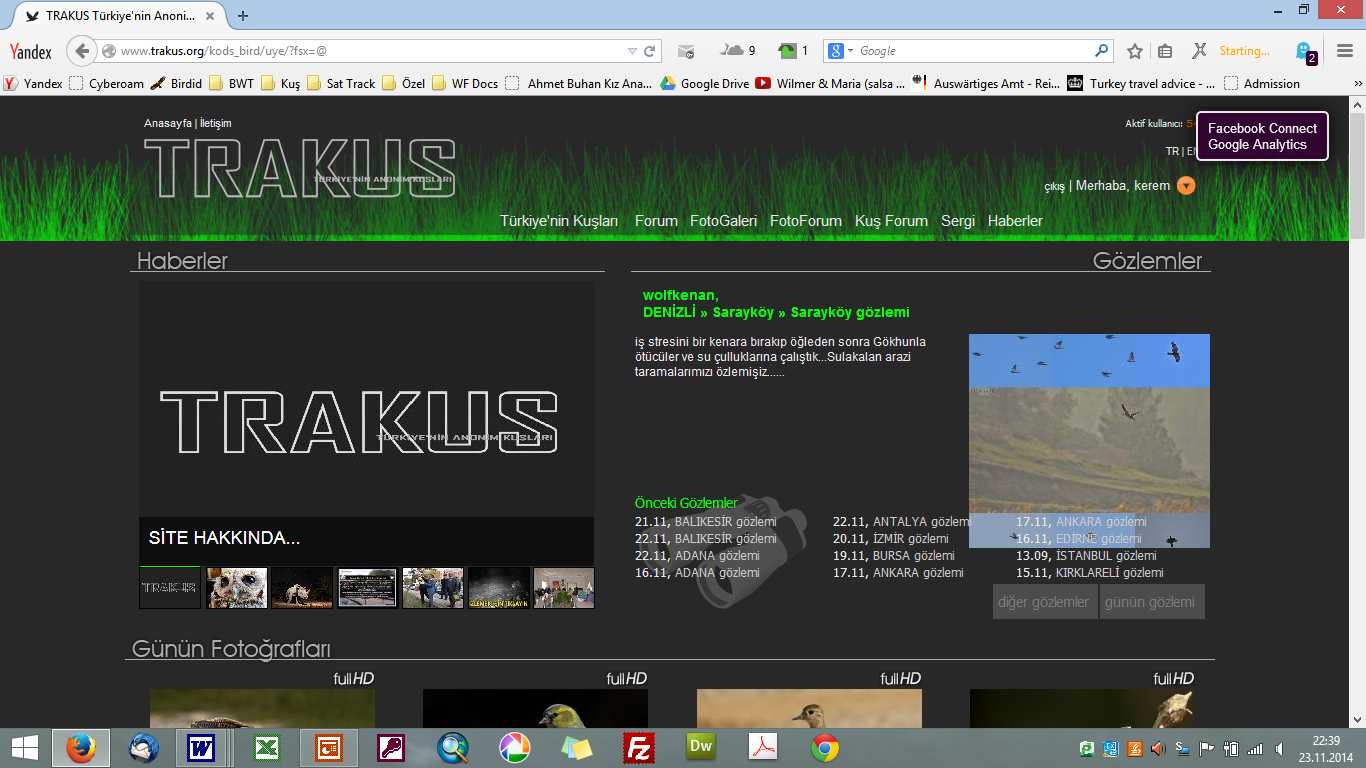
\includegraphics[keepaspectratio]{images/trakus.png}}

}

\caption{TRAKUS portalı. http://www.trakus.org}

\end{figure}%

\textbf{Halkalama}

Ötücü kuşlar ve yağmurcunların halkalanması, Türkiye'de ilk kez WIWO'nun
Çukurova (Kivit, Nijmeijer \& Ovaa, 1994) ve Kızılırmak Deltası
(Hustings \& Dijk, 1994) projeleriyle başlamış olup, 2002 yılında ulusal
halkalama programının başlatılmasıyla Ankara, Manyas, Manavgat, Kars,
Diyarbakır ve Kızılırmak Deltası gibi alanlarda ilkbahar ve sonbahar
dönemlerinde halkalama yapılmaya başlanmıştır. Programdaki en eski ve
sürekli çalışan istasyon, Kızılırmak Deltası'ndaki Cernek Halkalama
İstasyonu'dur (Barış \emph{vd.}, 2005). Zamanla bazı istasyonlar düzenli
çalışmasa da Kızılırmak Deltası, Kars ve Antalya'da halkalama
çalışmaları devam etmektedir. Uluslararası projeler kapsamında su
kuşlarının kuş gribine katkısını araştırmak amacıyla su kuşları
halkalanmış, örneklenmiş ve bazı bireyler uydu vericileriyle takip
edilmiştir. Ayrıca 2003-2009 yılları arasında İzmir Tuzla'da yapılan beş
flamingo halkalama çalışması, Akdeniz'deki flamingo popülasyonlarına
dair önemli veriler sağlamıştır (Balkız \emph{vd.}, 2009).

\bookmarksetup{startatroot}

\chapter*{Bilgi Kaynakları ve
Boşlukları}\label{bilgi-kaynaklarux131-ve-boux15fluklarux131}
\addcontentsline{toc}{chapter}{Bilgi Kaynakları ve Boşlukları}

\markboth{Bilgi Kaynakları ve Boşlukları}{Bilgi Kaynakları ve
Boşlukları}

Hazırlayanlar: Geoff Welch, Hilary Welch and Sancar Barış (2005)

1990 ile 2005 yılları arasında, Türkiye'nin kuşları hakkındaki
bilgilerimiz, yerel kuş gözlemciliğinin ve doğa koruma topluluklarının
gelişmesine paralel olarak önemli ölçüde ilerlemiştir. Bu bölüm,
Türkiye'nin kuşlarıyla ilgili bilgimizi sınırlayan, bazıları genel
bazıları ise oldukça spesifik olan temel sorunları tanımlarken aynı
zamanda geleceğe yönelik olarak Türk kuş faunasına dair atılabilecek
önemli adımları ortaya koymaktadır.

\textbf{Türlerin Yayılışı}

Gözlem haritaları, Kuşların yayılışı mı, yoksa kuş gözlemcilerinin mi?
Yakın zamana dek, Türkiye kuş veri havuzu büyük ölçüde tatil için Batı
Avrupa'dan gelen kuş gözlemcilerinin katkılarıyla oluşuyordu. Ülkeyi
ziyaret eden yabancı gözlemciler, kısa süreli tatilleri boyunca mümkün
olduğunca çok tür ve çeşitli yaşam ortamı görmek isterler. Bu durum
önemli ölçüde taraflı bir veri oluşturur; çünkü gözlemciler her zaman
aynı yerlere, yılın aynı dönemlerinde giderek hep aynı kuş türlerini
gözlemler.

Türkiye'de kuş gözlemciliğinin gelişmesiyle bu sıkıntı büyük ölçüde
azalmıştır. Ancak bu kez de yerli kuş gözlemcilerinin gözlem alanları
genellikle yaşadıkları bölgeyle sınırlı kalmakta; bu durum, veri
toplamada daha geniş bir yelpazeye ulaşmak adına farklı yöntemlerin
geliştirilmesi gerekliliğini doğurmaktadır.

\textbf{Standart Verinin Eksikliği}

1998 ile 2003 yılları arasında Türkiye'nin geniş alanlarında, standart
yöntemlerle üreyen kuşlar hakkında veri toplayan üç önemli proje
yürütülmüştür: Konya Havzası'nda (Eken \& Magnin 1999), Akdeniz
ormanlarında (Zeydanlı ve ark. 2005) ve Güneydoğu Anadolu'da (Welch
2004). Bu çalışmalar sayesinde, ilk kez, araştırma alanları nadir
türlerin varlığı ya da kuşların yoğunlaştığı alanlar gibi önceki
bilgilere bağlı kalınmadan tarafsız bir şekilde belirlenmiştir. Elde
edilen veriler kuşların kesinlikle nerelerde bulunduğunu göstermenin
yanı sıra neredeyse nerelerde bulunmadıklarını da ortaya koymuştur.
Ancak, bu tür çalışmalar önemli ölçüde daha fazla insan gücü gerektirir,
organize edilmesi zordur ve nispeten pahalıdır.

Yaygın türlerin yayılışı, gözlemcilerin bilinçsizce her yerde var
olduklarını düşündükleri kargalar, toygarlar, serçeler, sığırcıklar ve
evcil güvercinler gibi kuşları yeterince kaydetmemelerinden dolayı eksik
kalmaktadır. Örneğin, kumru her yerde bulunduğu varsayılan, hareket
halindeki bir araçtan bile kolayca gözlemlenebilecek bir tür olarak
bilinir. Ancak 2005 yılında ülkenin kuzeybatısında yapılan iki haftalık
saha çalışmasında Erzurum'un kuzeyinde bulunmadığı, Kars'ta hiç
kaydedilmediği ve ancak Yeşilırmak ovasında tekrar ortaya çıktığı tespit
edilmiştir.

\textbf{Üreme Durumu}

Kızıl Sırtlı Örümcekkuşu, Türkiye'deki kuşların yayılışının gözlem
verileriyle nasıl doğrulandığına iyi bir örnek teşkil eder. Bu tür, göç
dönemlerinde oldukça yaygın görülür ve çoğu kuş kitabı ile arazi
rehberinde Türkiye'nin geniş bir alanında üreyen bir tür olarak
tanıtılır. Ancak bu gerçekten böyle mi? Kızıl Sırtlı Örümcekkuşu'nun
(göç başlangıç ve bitiş tarihleri tam olarak belirlenemeyen) uzun bir
göç dönemi vardır. Ağustos 2005 itibarıyla Kuşbank veritabanındaki 313
kaydın 128'i (\%41) bir üreme koduyla ilişkilendirilmişken, yalnızca
yedisinde (\%2) kesin üremeye dair itiraz edilemez kanıt bulunmaktadır.
Geriye kalan 121 kaydın büyük bir kısmı, özellikle de 35 tanesi dışında
olanlar, muhtemelen göç eden bireylere aittir. Bazı durumlarda birkaç
dakikalık bir gözlem, ``olasılık'' düzeyinde bir üreme kaydını
``muhtemel'' veya ``kesin'' üreme kaydına dönüştürebilir.

\textbf{Su Kuşu Sayımları}

1986'dan itibaren IWRB/Wetlands International tarafından organize edilen
Kış Ortası Su Kuşu Sayımları (KOSKS), Türkiye'de uzun süreli su kuşu
verisi sağlamakta önemli bir rol oynamıştır. Ancak, bu program on
yıllardır sürdürülse de sayım metodolojisinde çeşitli değişkenlikler
gözlenmiştir: ziyaret edilen alanların sayısı, her bir alanın kapsanma
şekli, katılımcı sayısı ve deneyim seviyeleri yıllar içinde değişmiştir.
Bu yüzden, kışlayan kuş sayılarındaki artış veya azalışı incelemek için
yapılan çalışmalarda veri toplama yöntemindeki bu değişikliklerin de
dikkate alınması gerekmektedir. Belirli bir türün sayısındaki değişim,
gerçekten popülasyon artışına ya da azalmasına mı işaret etmektedir,
yoksa bu farklı yıllarda sayılan alanların kapsamı mı değişmiştir? Söz
konusu türün tespit zorluğu, alanların bazı yıllarda daha detaylı ya da
yüzeysel sayılması, sayım sonuçlarını etkileyebilir. Ayrıca, Türkiye
veya Doğu Avrupa-Rusya-Orta Asya'daki hava koşulları ve avcılık baskısı
gibi kontrol edilemeyen değişkenler de kuşların dağılımını
etkileyebilir.

2012 yılında kurulan Ulusal KOSKS Kurulu, bu sayımları daha kapsamlı ve
standart hale getirmeyi hedeflemiştir. Sayım yapılacak alanların
kapsamı, önemi ve isimlendirilmesi standartlaştırılmış; sabit sayım
istasyonları belirlenmiştir. Tüm metotlar ve protokoller, formlar ve
haritalarla birlikte kullanıma sunulmuştur. Ayrıca gözlem verilerinin
sistematik olarak Kuşbank'a kaydedilmesi, verilerin doğruluğunu
sağlamakla birlikte raporlamayı da kolaylaştırmıştır. KOSKS Kurulu daha
sonra dağılmıştır.

Bir alanı kullanan kuş sayısının mevsimden mevsime veya yıldan yıla
değişim göstermesi doğal bir durumdur. ÖKA (Önemli Kuş Alanı) olarak
belirlenmesi gereken bir alan, kötü bir yılda gözden kaçabilir veya
komşu alanlarda normalin dışındaki su seviyeleri nedeniyle geçici olarak
yüksek sayıda kuş barındırabilir. Bu tür durumlar, yalnızca sulakalanlar
ağındaki işleviyle önemli olan bir alanın, koruma açısından en öncelikli
yerlerden biri olarak değerlendirilmesine yol açabilir.

\textbf{Gözden Kaçan Türler}

Bazı kuşlar daha çok dikkat çekerken bazıları ise gözlenmeden
varlıklarını sürdürebilir. Gececil kuşlar özel teknikler kullanılmadıkça
olduğundan daha az kayda geçer. Saklanan ve ürkek türler bolca
bulunmalarına rağmen fark edilmeyebilir. Örneğin, Paçalı Baykuş, aslında
Türkiye'de nispeten yaygın olabilecek bir türdür, ancak 25 yıl öncesine
kadar hiç kaydedilmemiştir.

Koloni halinde üreyen türler, uygun yaşam alanı bulsalar bile düzensiz
bir dağılım sergileyebilirler. Bazı türler ise erişilmesi zor, uzak
bölgelerde yaşadığından tespiti zorlaşır. Koloniler bir kez
keşfedildiğinde popülasyonu izlemek kolaylaşsa da, yeni koloniler bulmak
zorludur. Örneğin, İspir'deki kızıl akbaba kolonisi, yola yakın
kayalıklarda bulunduğu için bilinirken, komşu vadilerdeki potansiyel
koloniler hakkında bilgi yoktur.

Alpin türler genellikle parçalı bir yayılış gösterir, düşük yoğunlukta
bulunurlar ve bölgede kısa süre kalabilirler. Bu nedenle, yükseklerde
yaşayan kuşların dağılımını yeterince bilmek güçtür.

Kuş türlerinin seslerinden tanınması ise ayrı bir zorluk sunar.
Türkiye'deki kuş gözlemcileri ötüşle tanıma konusunda nispeten az
deneyimlidir. Ayrıca, bölgesel alttür ve ırkların ötüşleri hakkında
bilgi eksikliği de bulunur. Türkiye'de üreyen Kızılkuyruk, deneyimli
Avrupalı gözlemciler tarafından bile bazen Şakrak ile karıştırılır. Boz
Kirazkuşu gibi türler de ötüşleriyle benzer türlerle karışabilir ve
yaygın oldukları bölgelerde gözden kaçabilirler.

\textbf{Popülasyon Tahminleri}

Batı Avrupa'da her tür için güvenilir, bazen oldukça kesin popülasyon
rakamları mevcut olup, bu veriler koruma eylemlerinin uygulanmasına ve
Avrupa Birliği düzeyinde uzun vadeli koruma politikalarının
geliştirilmesine katkı sağlamaktadır.

Türkiye'de ise güvenilir kalitatif bilgiler ya çok sınırlıdır ya da eski
kalmıştır. Ülkenin genişliği, sınırlı sayıda yerli kuş gözlemcisinin
varlığı ve yurt dışından gelen gözlemcilerin aksine sistematik
araştırmalara katılmak için deneyim, zaman, finansal kaynak ve seyahat
imkanı kısıtlılığı, gözlemcilerin çalışmalarını zorlaştırmaktadır.
Akademik düzeyde kuşlarla ilgili ilgi ise oldukça yenidir ve yalnızca
birkaç tane uluslararası standartlarda yüksek lisans ve doktora tezi
tamamlanmıştır.

Toy, Leylek, Kara Akbaba ve Dağ Horozu gibi yüksek koruma değerine sahip
türler için çeşitli araştırmalar yapılmakta veya devam etmektedir. Bu
çalışmalarda, halktan gelen bilgiler (Leylek), radyo vericileriyle
izleme (Kara Akbaba) ve bilgisayar destekli modellemeler (Dağ Horozu)
gibi farklı yöntemler kullanılmaktadır. Ancak çoğu tür için yalnızca
``en iyi tahmin'' düzeyinde verilere sahibiz. Türkiye'de, Birecik'teki
yarı evcil kelaynak kolonisi haricinde, hiçbir tür için güvenilir
popülasyon tahmini bulunmamaktadır.

Kuş gözlemcileri için sulakalanlar, kuş çeşitliliği ve gözleme kolaylığı
nedeniyle cazip alanlardır ve gözlemlerden elde edilen kayıtların çoğu
bu alanlardan gelmektedir. Ancak, yıllar içinde bu sulakalan odaklı
gözlem eğilimi, Devlet Su İşleri'nin 1930'lardaki master planlara uygun
olarak sulakalanları kurutup baraj inşa etmesiyle, hızla kaybolan türler
ve habitatlar listesine dönüşmüştür.

\textbf{Göç Sayımları}

Gündüz yırtıcılarının ve diğer süzülen kuşların görünür göçü Türkiye'de
uzun zamandır biliniyor olsa da, bu göçün sürdürülebilir ve eşgüdümlü
olarak izlenmesi için yapılan çalışmalar oldukça sınırlıdır. 1960'lar ve
70'lerde İstanbul Boğazı, Kuzey-Batı Türkiye ve İskenderun Körfezi'nde
gündüz yırtıcılarının ve süzülen kuşların gözlenmesi (Porter \& Willis,
1968; Beaman, 1977; Beaman \& Porter, 1977; Sutherland \& Brooks,
1981a), batılı kuş gözlemcilerinin Türkiye'deki bu önemli göçün farkına
varmasını sağlamış ve büyük bir ilgiyle Türkiye'yi ziyaret etmelerine
vesile olmuştur.

Görülebilir göç sayımı, uzun süreli yoğun konsantrasyon ve disiplin
gerektiren bir iş olup, kendini işe adamış az sayıda gözlemci tarafından
gerçekleştirilir. Bu nedenle, dünyada düzenli ve uzun süreli gündüz
yırtıcı göçü çalışmaları oldukça sınırlıdır. Ayrıca, elde edilen
verilerin koruma değerinin belirginleştirilmesi zor olduğundan, yırtıcı
sayımları için mali kaynak bulmak da kolay değildir. Yine de, süzülen
kuş göçü görsel açıdan oldukça etkileyici bir doğa olayıdır ve toplumun
doğal çevreye olan ilgisini ve korunma gereksinimine dair farkındalığını
artırmak için güçlü bir araçtır; bu nedenle, önemi göz ardı
edilmemelidir.

\textbf{Halkalama İstasyonları}

Ötücü kuşlar ve yağmurcunların halkalanmasını içeren çalışmalar,
Türkiye'de ilk olarak WIWO'nun 1990'da Çukurova (Kivit \emph{vd.}, 1994)
ve 1992'de Kızılırmak Deltası'nda (Hustings \& Dijk, 1994) yürüttüğü
çalışmalarında başlamıştır. 2002 yılında ulusal halkalama programının
hayata geçirilmesiyle birlikte eğitimli halkalamacılar yetiştirilmiş ve
Ankara, Manyas, Manavgat, Kars, Diyarbakır ve Kızılırmak Deltası'nda
ilkbahar ve sonbaharda halkalama yapılan bir program oluşturulmuştur. Bu
programdaki en eski ve sürekli çalışan istasyon, Kızılırmak
Deltası'ndaki Cernek Halkalama İstasyonu olmuştur (Barış \emph{vd.},
2005).

Bu tür çalışmaların uzun vadeli koruma açısından sağladığı en önemli
yarar, konaklama alanlarını kullanan kuş sayılarındaki değişimlerin ve
popülasyon hareketlerinin izlenmesine olanak tanımasıdır. Böylelikle her
alanın kuşlar açısından taşıdığı gerçek önem ortaya konulabilir. Sürekli
ve standart çalışan halkalama istasyonları, Türk ornitolojisine sadece
veri sağlamakla kalmayıp, uzun vadede daha kapsamlı katkılar
sunmaktadır.

\textbf{Kuşbank ve eBird}

Türkiye için elde edilen tüm bilgilerin erişilebilir ve koruma
çalışmalarına katkı sağlayacak bir formatta saklanması büyük önem taşır.
Bu amaçla, 2001 yılında kurulan ve 2004'te kullanıma açılan KuşBank
ağ-temelli veri tabanı geliştirilmiştir. KuşBank, kuş gözlemcileri
tarafından geniş kabul görmüş ve oldukça başarılı olmuştur. Kasım 2005
itibarıyla, veritabanına 350 gözlemci tarafından 400 türe ait 97.000'den
fazla kayıt girilmiştir. Ancak verilerin gerçek anlamda değerli
olabilmesi için kalite güvence altına alınmalıdır. Bu nedenle, belirli
standartların karşılandığından emin olmak amacıyla bir Kayıt Komitesi
oluşturulmuştur. Başlangıçta sadece KuşBank'a girilen kayıtları
değerlendiren bu komitenin, zamanla ulusal ölçekte nadir türlerin
kayıtlarını inceleyen bir komiteye dönüşmüştür.

\pandocbounded{
\includegraphics[keepaspectratio]{images/kusbank.png}}

\textbf{Türkiye Üreyen Kuş Atlası}

Türkiye kuşları hakkında yöntemselliğe dayalı nitelikli çalışmalar ve
güvenilir verilerle koruma önceliklerini belirleyebilme gereksinimi,
bugün hala aşılması gereken önemli bir sorun olarak karşımızda
durmaktadır. Türkiye'de yöntemsel çalışmaları bağımsız olarak
yürütebilecek kuş gözlemcilerinin sayısı yüz civarında olsa da,
metindeki tespitler ve eleştiriler geçerliliğini korumaktadır. Bu
bağlamda, kuş gözlemcilerinin katkılarının koruma çalışmalarına daha
etkili yansıması için stratejik yaklaşımlar geliştirilmesi önemlidir.
Koruma liderlerinin öncelikli alanlar, türler ya da veri eksikliklerini
sistematik olarak belirlemeleri ve giderek artan akademik kapasiteye
sahip üniversitelerle iş birliği yapmaları, kuş gözlemcilerinin veri
açıklarını kapatma konusunda daha verimli olmasını sağlayabilir. Kış
Ortası Su Kuşu Sayımları'nın analiz edilmesi, ulusal düzeyde bilgi
sağlayacak bir yaygın kuş gözlem programının yaygınlaştırılması ve
dinamik bir kuş atlasının oluşturulması hala gerçekleştirilmesi beklenen
adımlar arasında yer almaktadır.

Not: Bu yazı yazıldıktan sonra 2018 yılında Türkiye Üreyen Kuş Atlası
çalışması tamamlanmıştır!

\part{Ötücü Olmayanlar}

\chapter{Ördekgiller}\label{uxf6rdekgiller}

\section{Boz Kaz}\label{boz-kaz}

\emph{Anser anser}, Greylag Goose

\textbf{\emph{Lokal olarak az sayıda ürer. Kışın göç alır ve daha geniş
bir alanda yayılış gösterir.}}

Üreme döneminde az sayıda Göller Bölgesi, İç Anadolu ve Doğu
Anadolu'daki bataklık sulakalanlarda bulunur. Sultansazlığı gibi birkaç
alanda eskiden yüksek sayılarda üremiştir. Türkiye Kuş Raporları üreyen
popülasyonun son 50 yılda çok ciddi bir düşüş yaşadığını göstermektedir
(OST, 1969, 1972, 1975, 1978; Beaman, 1986; Martins, 1989; Kirwan \&
Martins, 1994, 2000; Kirwan \emph{vd.}, 2003; Kirwan, Özen \& Demirci,
2009; Kirwan \& Özen, 2014). Eskiden ürediği sulakalanların çoğu
kurutulmuştur. Örneğin, Ereğli Sazlığı'nda Nisan 1970'te 120 yuva ve 300
birey varken Temmuz 1996'da 160 birey sayılmış, bugün ise hiçbir üreyen
çift kalmamıştır.

Üreme sonrasında tüy dökümü sırasında kalabalık sürüler bazı
sulakalanlarda toplanır; Temmuz 1984'te Kulu Gölü'nde 800 birey,
bilinmeyen bir tarihte Sultansazlığı'nda 12.000 birey ve Eylül 2004'te
Kuyucuk Gölü'nde 10.000 birey kaydedilmiştir.

Geçiş sırasında tüm bölgelerde görülen ve ekimden itibaren mart sonuna
kadar kalan bir kış göçmenidir. Kışlayan sürüler genellikle kıyısal
bölgelerde yoğunlaşır. Son yıllarda görülen sürüler 300 bireyden azdır.
KOSKS verilerine göre eskiden daha bol bulunduğu bilinmektedir. Ülke
genelinde ortalama 5000 birey, en yüksek ise 1967'de 11.200 birey olarak
sayılmıştır. Alanlarda yapılan sayımlarda Kızılırmak Deltası'nda 5000
birey, Meriç Deltası'nda 4500 birey ve Hotamış Sazlığı'nda 1500 birey
tespit edilmiştir.

\pandocbounded{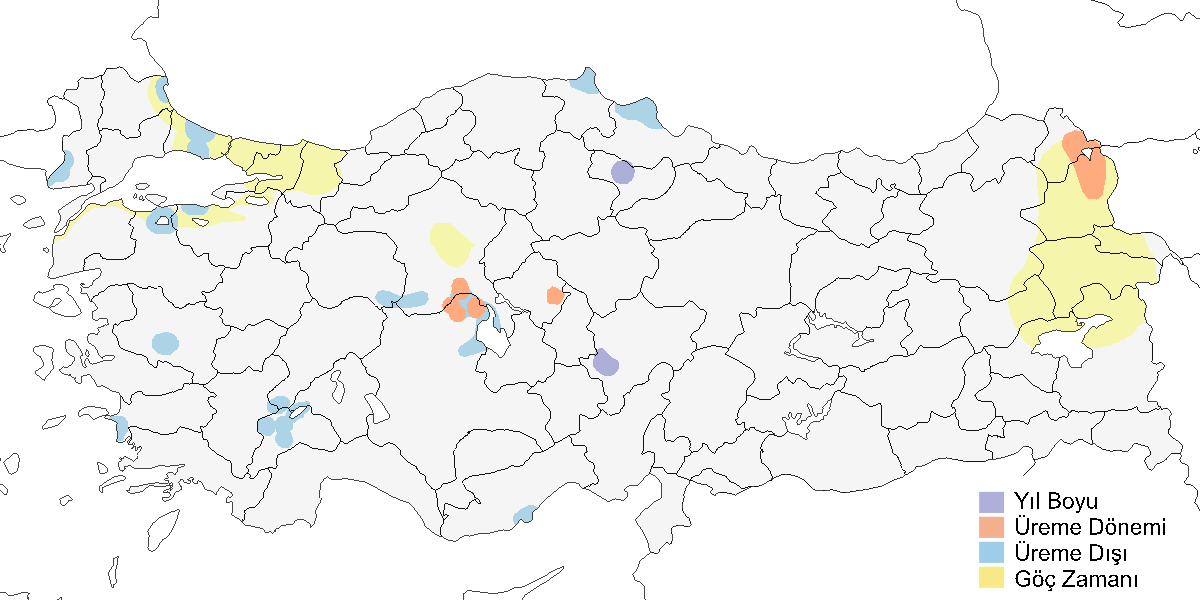
\includegraphics[keepaspectratio]{images/harita_Anser anser.png}}

\textbf{Üreme}

\textbf{Yuvalama Alanı:} Göllerdeki adalarda genellikle küçük gruplar
halinde ürer.\\
\textbf{Yuvası:} Kulu Gölü'nde gözlenen yuvası kuru toprağa kazılmış sığ
bir çukurdur ve çevredeki bitki örtüsü ile küçük tüylerle
astarlanmıştır. Ereğli Sazlığı'ndaki yuvası ise saz ve diğer sucul
bitkilerden oluşan, su seviyesinin üstünde kalan bir yapının üzerine
kurulmuştur.\\
\textbf{Yumurta Sayısı:} Türkiye'de yumurta sayısına ilişkin güvenilir
gözlem yoktur. Yuvadan ayrılmış beş yavru, en az beş yumurta koyduğunu
gösterir. Diğer ülkelerde genellikle 4-6 yumurta bırakır.\\
\textbf{Üreme Dönemi:} Mart sonunda yumurta koyar. En erken yavrular 23
Nisan 1988'de Kulu Gölü'nde, 27 Nisan 1988'de Sultansazlığı'nda, 30
Nisan 1968'de Mogan Gölü'nde ve 30 Nisan 1973'te Ereğli Sazlıkları'nda
gözlenmiştir. 20 Nisan 1996'da Marmara'da, 14 Mayıs 1969'da
Karadeniz'de, 16 Mayıs 1970'te ve 24 Haziran 1983'te Doğu Anadolu'da
kaydedilen yavrular gecikmiş üremeyi göstermektedir.

\textbf{Alttürler ve Sınıflandırma}

Ülkemizde \emph{rubrirostris} alttürü bulunur. Bu alttür turuncu
gagasıyla Batı ve Orta Avrupa'da bulunan pembe gagalı \emph{anser}
alttüründen ayrılır.

\section{Sakarca}\label{sakarca}

\emph{Anser albifrons}, Greater White-fronted Goose

\textbf{\emph{Lokal olarak bulunan ve zaman zaman kalabalık sürüler
oluşturan bir kış konuğudur.}}

Ekim sonu ile nisan başı arasında lokal olarak görülen bir kış
konuğudur. Genellikle ocak ve şubat aylarında daha yaygın ve yüksek
sayıda olur. Soğuk geçen kışlarda Türkiye'de kışlayan birey sayısı
artar. En kalabalık sürüler Meriç Nehri boyunca, Tuz Gölü çevresinde ve
Konya Ovası'nda yoğunlaşır. Büyük Menderes Deltası ve Doğu Akdeniz'deki
sulakalanlarda da önemli sayılarda toplanabilir. Son zamanlarda
Güneydoğu Anadolu'daki baraj göllerinde küçük sürüler halinde görülmeye
başlanmıştır. Nadiren yaz aylarında sulakalanlarda az sayıda birey
kalabilir.

Kış ortası su kuşu sayımlarında (KOSKS) ülke genelinde en yüksek sayı
1968-69 kışında 98.600 birey olarak kaydedilmiştir. 1987'de ise toplam
84.000 birey sayılmıştır. Ancak daha sonra kışlayan birey sayısında
ciddi bir düşüş yaşanmıştır. 1990'lı yıllarda genellikle 20.000-30.000
arasında değişen sayılar kaydedilmiş 1993'te 11.822 (DHKD, 1993),
1999'da 3956 (DHKD, 1999) ve 2005'te 3891 birey (Çağlayan \emph{vd.},
2005) tespit edilmiştir. Kışın soğuk geçtiği 11 Şubat 2006'da
Büyükçekmece'de 15.000 birey sayılmıştır, bu da son yıllardaki en yüksek
sayıdır. Dolayısıyla Türkiye'de kışlayan nüfusun 1970'lerde 100.000'ler
seviyesinden 2010'larda 5000 civarına indiği söylenebilir.

\pandocbounded{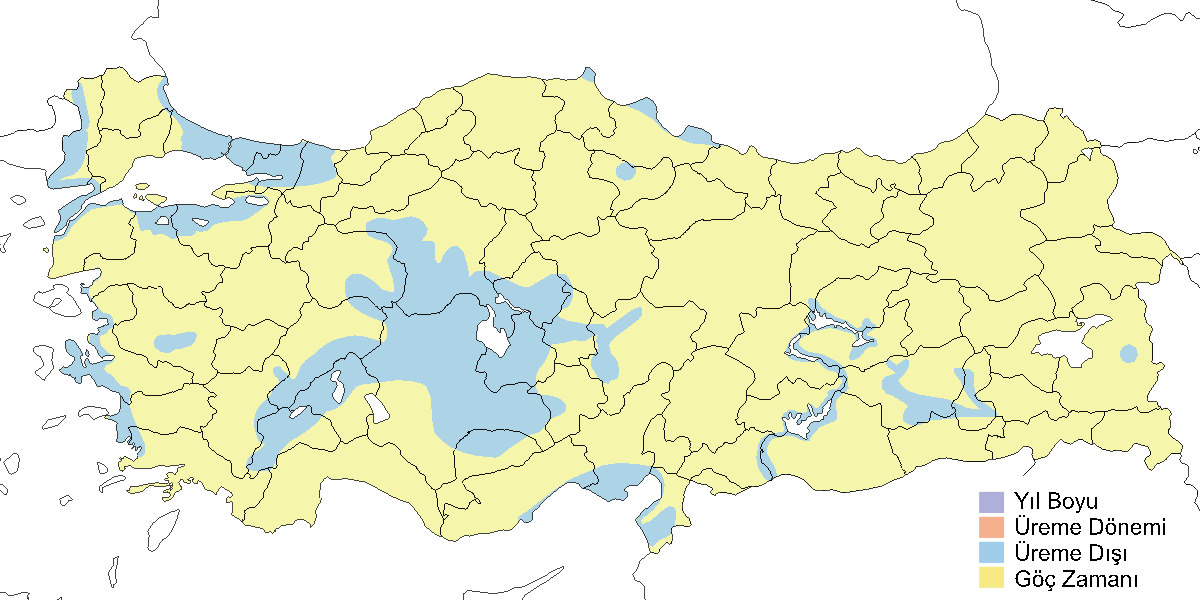
\includegraphics[keepaspectratio]{images/harita_Anser albifrons.png}}

\textbf{Üreme}

Türkiye'de yuvalamaz. Avrasya ve Kuzey Amerika'nın tundra bölgelerinde
yuvalar.

\textbf{Alttürler ve Sınıflandırma}

Türkiye'de nominat alttürü bulunur.

\section{Küçük Sakarca}\label{kuxfcuxe7uxfck-sakarca}

\emph{Anser erythropus}, Lesser White-fronted Goose

\textbf{\emph{Az sayıda gelen düzenli kış konuğudur.}}

Her yıl çok az sayıda kaydedilen bir kış konuğudur. Sayıları genellikle
10'dan azdır ve diğer kaz türleriyle karışık olarak görülebilir. Bugüne
kadar Türkiye'ye gelen bireylerin İskandinavya'da üreyen ve Balkan
ülkelerinde kışlayan göç yoluna ait olduğu düşünülmüştür. Yunanistan'da
bir alanda kışlayan ve koruma çalışmaları sayesinde sayıları artan bir
sürünün kış ortasında oradan kaybolması, Marmara ve Ege bölgelerinde bir
kışlama alanı olabileceği ihtimalini doğurmuştur. Ancak yapılan
aramalara rağmen burada düzenli kullanılan bir kışlama alanı
bulunamamıştır.

Doğu Anadolu'da 20 Kasım 2004'te Haçlı Gölü'nde uydudan izlenen bir
birey sinyal verince, doğuda bir kışlama alanı olasılığı gündeme
gelmiştir (Morozov \& Aarvak, 2004). Nitekim Van Gölü ve Erçek Gölü
kıyılarında sayıları 340'a ulaşan sürüler düzenli olarak tespit
edilmiştir. Bugün, Türkiye'de kışlayan ana nüfusun Doğu Anadolu'da
bulunduğu söylenebilir ((AOU), 2000).

2000 öncesindeki kayıtlara bakıldığında; 29 Aralık 1997'de Göksu
Deltası'nda bir birey (Kirwan \emph{vd.}, 2003), 23 Ocak 1993'te Göksu
Deltası'nda bir birey (DHKD, 1993), 6 Nisan 1990'da Seyfe Gölü'nde 12
birey (Kirwan \& Martins, 1994), 24 Aralık 1986'da Bafa Gölü'nde bir
erişkin ve iki genç birey (Kasparek, 1988a) ve 16 Şubat 1967'de Kocabaş
Çayı'nın ağzında (Çanakkale) iki birey (OST, 1969) kaydedilmiştir. 1945
ile 1965 yılları arasında ve ekim ile ocak aylarında, çoğunluğu
Büyükçekmece ve Küçükçekmece Göllerinden gelen 12 kayıt vardır. Ancak bu
kayıtlar, tür tanımını destekleyecek belgeden yoksundur (Kumerloeve,
1970a).

\pandocbounded{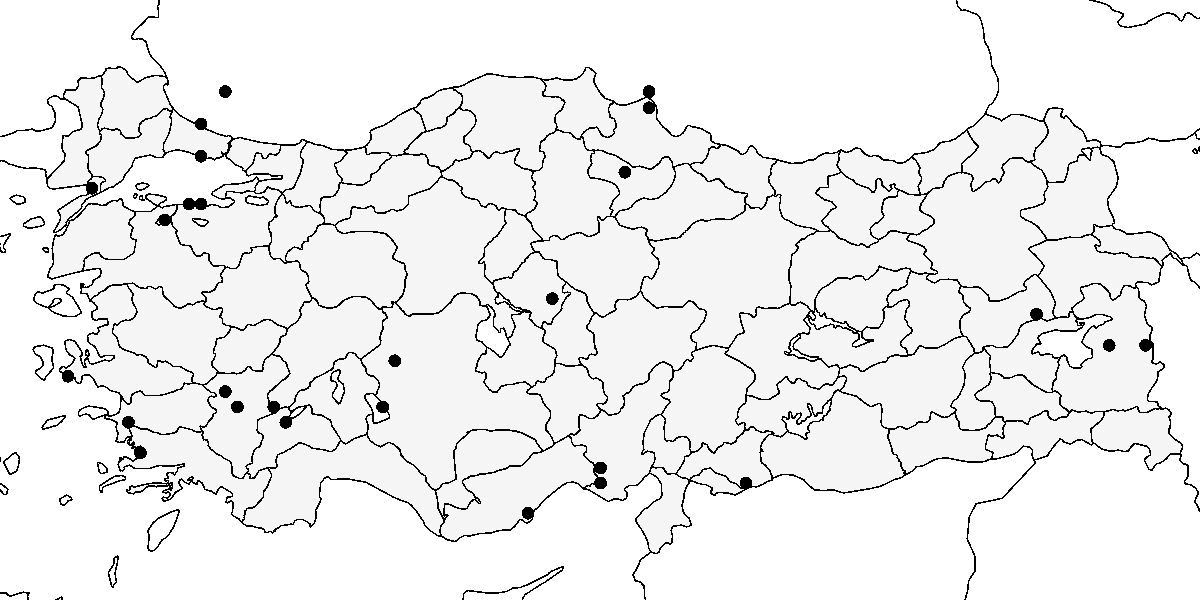
\includegraphics[keepaspectratio]{images/harita_Anser erythropus.png}}

\textbf{Üreme}

Türkiye'de yuvalamaz. Kuzey İskandinavya'dan Doğu Sibirya'ya kadar
uzanan tundra kuşağında ürer.

\textbf{Alttürler ve Sınıflandırma}

Monotipik bir türdür.

\section{Tundra Kazı}\label{tundra-kazux131}

\emph{Anser serrirostris}, Tundra Bean Goose

\textbf{\emph{Nadiren gelen kış konuğudur.}}

2000 yılından sonra 5 kez kaydedilmiştir. 26 Şubat 2013'te Yedikır
Barajı'nda, 4-21 Şubat 2015'te Kızılırmak Deltası'nda birer birey
görülmüştür. 31 Ocak 2016'da Manyas Kuş Gölü'nde 3 birey kaydedilmiş,
aynı alanda 2-24 Ocak 2019'da yine 3 birey gözlenmiştir. Acıgöl'de 24
Aralık 2023 ile 3 Şubat 2024 arasında bir birey gözlenmiştir.

\emph{Tundra Kazı}, önceleri \emph{Tayga Kazı} ile beraber tek bir tür
altında \emph{Tarla Kazı} olarak sınıflandırılıyordu. Dolayısıyla,
taksonomik revizyonun yapıldığı tarihten önceki kayıtlarda \emph{Tarla
Kazı} olarak tanımlanmıştır. 2000 yılından sonra çekilen fotoğraflarda
özellikle gaga renklenmesi incelenmiş ve bu kuşların tamamı \emph{Tundra
Kazı} olarak tanımlanmıştır. Fotoğrafı veya betimlemesi olmayan eski
kayıtların hangi türe ait olduğu ise belirsiz kalacaktır.

\emph{Tarla Kazı} olarak tanımlanmış kuşlar, Ege, Akdeniz ve İç
Anadolu'daki sulakalanlarda ara sıra yüksek sayılarda kaydedilmiştir.
1870'ler ve 1880'lerde Mersin'de toplanan bireyler (Schrader, 1891) ilk
kayıtlar arasındadır. 1966-2000 yılları arasında çoğunlukla ocak ile
mart ayları arasında 15 kez kaydedilmiştir. 2 Mart 1965'te Ereğli ve
Karapınar arasında 90 birey (Kumerloeve, 1970a), 15-16 Ekim 1969'da
Karamık Sazlıkları'nda 13 birey (OST, 1972), 30 Nisan 1988'de Seyfe
Gölü'nde, 30 Ocak 1992'de Marmara Gölü'nde 61 birey, 9 Ocak 1993'te
Büyükçekmece Gölü'nde 64 birey (DHKD, 1993) ve 24 Ocak 1993'te Göksu
Deltası'nda bir birey (DHKD, 1993) kaydedilmiştir. Türkiye'deki kışlayan
Sakarca sayılarındaki sert düşüş, muhtemelen \emph{Tarla Kazı} olarak
tanımlanmış kuşlar için de geçerlidir.

\pandocbounded{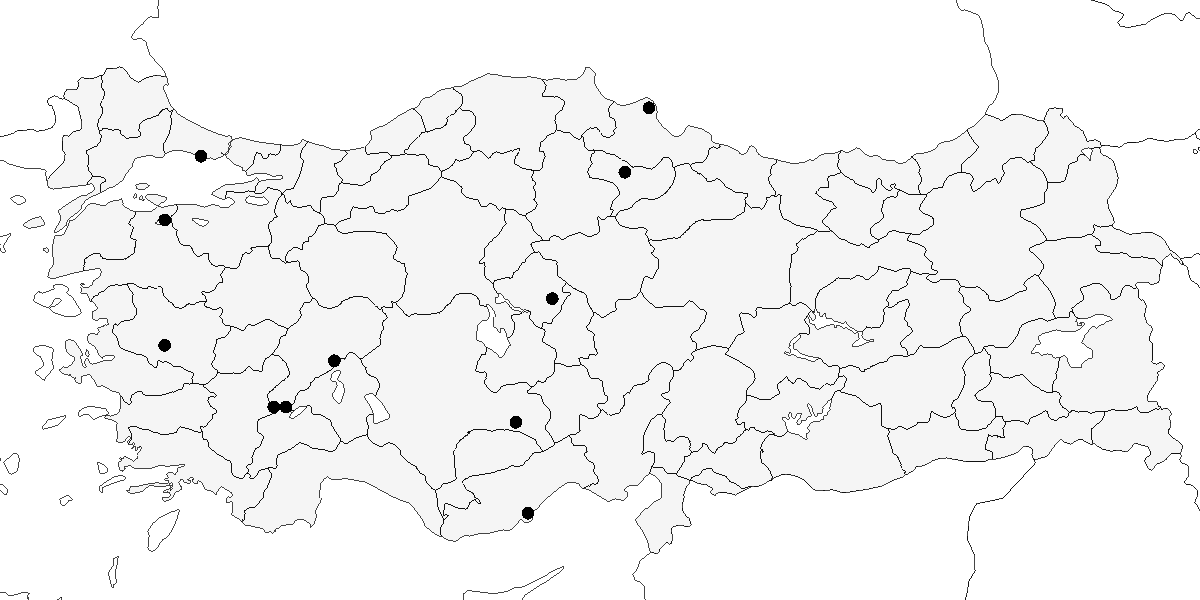
\includegraphics[keepaspectratio]{images/harita_Anser serrirostris.png}}

\textbf{Üreme}

Türkiye'de yuvalamaz. Üreme alanı Kuzey İskandinavya'dan Doğu Sibirya'ya
uzanan tundra kuşağındadır.

\textbf{Alttürler ve Sınıflandırma}

Tayga Kazı, yakın zamana kadar Tarla Kazı olarak bilinen bir türden
ayrılan yeni bir türdür. Beş alttüre sahip olan Tarla Kazı (\emph{Anser
fabalis}), iki gruba ayrılmıştır: \emph{fabalis}, \emph{johanseni} ve
\emph{middendorffii} alttürleri Tayga Kazı (\emph{Anser fabalis}),
\emph{serrirostris} ve \emph{rossicus} alttürleri ise Tundra Kazı
(\emph{Anser serrirostris}) olarak sınıflandırılmıştır.

\section{Yosun Kazı}\label{yosun-kazux131}

\emph{Branta bernicla}, Brant Goose

\textbf{\emph{Rastlantısal konuktur.}}

Batı Avrupa'nın Atlantik kıyılarında kışlayan bir türdür. Türkiye ile
yakın coğrafyasında rastlantısal bir konuktur. 6 Nisan 1981'de Küçük
Menderes Deltası'nda iki birey gözlenmiştir (Beaman, 1986). 3-4 Eylül
1973'te Ardeşen açıklarında koyu karınlı \emph{bernicla} alttürüne ait
iki birey kaydedilmiştir (OST, 1975). 1969 yılında Acıgöl'den gelen bir
iddia ise kabul edilmemiştir (Dijksen \& Kasparek, 1988). 7 Şubat
1945'te Büyükçekmece'de bir birey Prenses Zeyneb Halim tarafından
vurulmuştur, ancak kuşun gövdesi korunamamıştır (Kumerloeve, 1970a).
Ocak 1889'da kışın soğuk geçtiği bir yılda İstanbul Maltepe'de düzenli
olarak, Şubat 1891'de ise büyük sürüler halinde İstanbul Kadıköy'de
görülmüştür (Mathey-Dupraz, 1920--24).

\pandocbounded{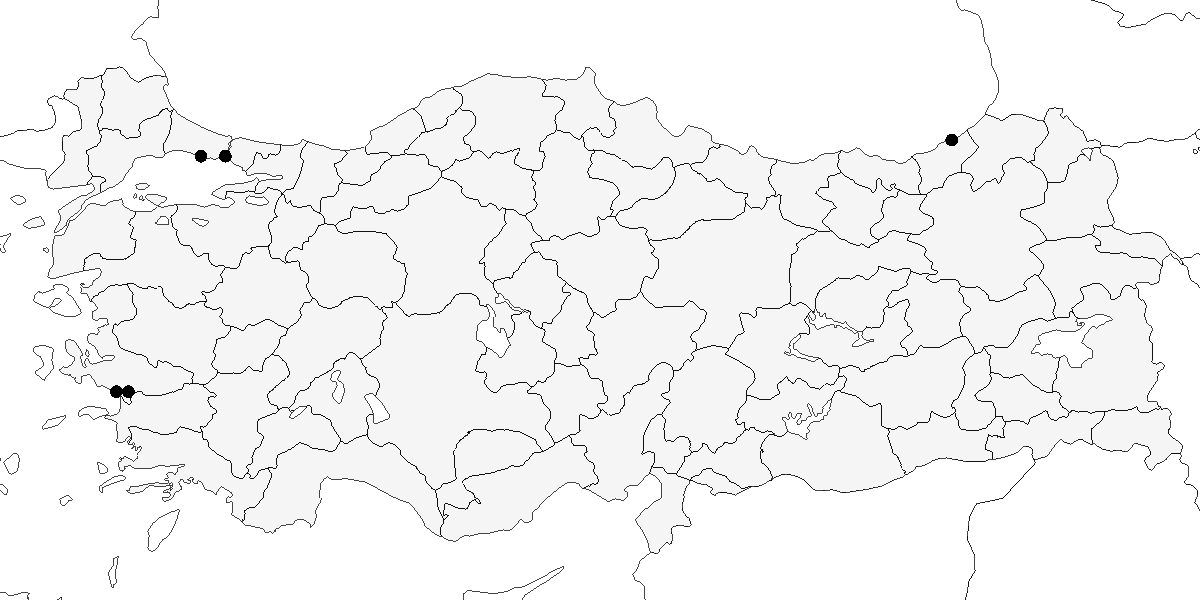
\includegraphics[keepaspectratio]{images/harita_Branta bernicla.png}}

\textbf{Üreme}

Türkiye'de yuvalamaz. Orta ve Kuzey Sibirya'nın Kutup Denizi kıyılarında
yuvalar.

\textbf{Alttürler ve Sınıflandırma}

Bir kayıtta kuşun alttürü \emph{bernicla} olarak tanımlanmıştır. Keza,
Kuzeybatı Avrupa'da kışlayan \emph{bernicla} alttürünün Türkiye'de
görülmesi olasıdır. Yunanistan'daki bir kayıt da bu alttüre aittir
(Handrinos \& Akriotis, 1997).

\section{Ak Yanaklı Kaz}\label{ak-yanaklux131-kaz}

\emph{Branta leucopsis}, Barnacle Goose

\textbf{\emph{Rastlantısal konuktur.}}

5 Ocak 2003'te Büyükçekmece Gölü'nde bir birey gözlenmiş ve detaylı
olarak belgelenmiştir. 1946/47 kışında Sakarya Deltası'nda bir birey,
1961 sonbahar/kışında ise başka bir birey vurulmuştur. İkinci kuşun
tahniti Eylül 1964'te Ankara'da bulunmuş, ancak sahibi tahniti satmaya
yanaşmamıştır (Kumerloeve, 1966a). Bu iki kaydın belgeleri yetersizdir
(Kumerloeve, 1970a).

\pandocbounded{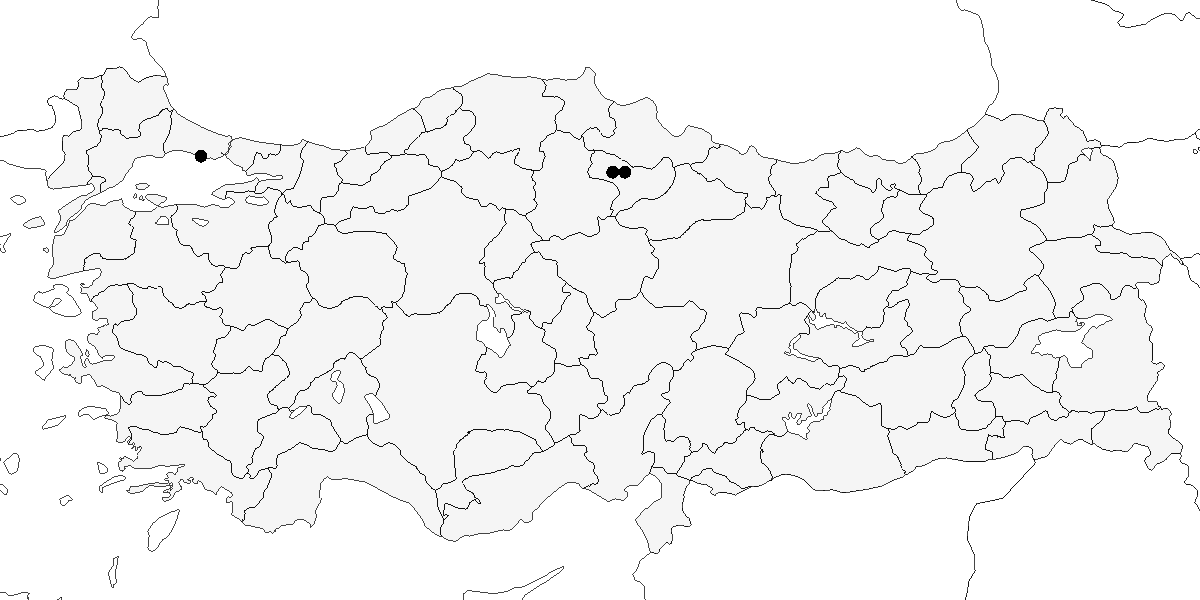
\includegraphics[keepaspectratio]{images/harita_Branta leucopsis.png}}

\textbf{Üreme}

Türkiye'de yuvalamaz. Grönland, İzlanda, Kuzey Batı Rusya ve Baltık
Denizi kıyılarında yuvalar.

\textbf{Alttürler ve Sınıflandırma}

Monotipik bir türdür.

\section{Sibirya Kazı}\label{sibirya-kazux131}

\emph{Branta ruficollis}, Red-breasted Goose

\textbf{\emph{Az sayıda gelen düzensiz kış konuğudur.}}

Türkiye'de düzenli kışladığı bilinen bir alan yoktur; ana kışlama alanı
Romanya ve Bulgaristan'ın Karadeniz kıyısıdır. Özellikle soğuk kışlarda,
bireyler veya gruplar halinde Türkiye'ye inerler. 1964 ile 2008 yılları
arasında 64 kayda rastlanmıştır. Bu kayıtların 15'i Marmara'da, 12'si İç
Anadolu'da, 8'i Karadeniz'de, 6'sı Akdeniz'de ve 4'ü Ege'de alınmıştır.
Kayıtların çoğu aralık sonu ile şubat başı arasındadır. Çoğunlukla bir
veya birkaç kuş sayılmış, ancak 5 kayıtta 40 ila 100 bireyden oluşan
nispeten kalabalık sürüler de gözlenmiştir. 2001/2002 kışında Türkiye
genelinde 192 birey sayılmıştır.

Ülke genelinde yaygın olarak av mağazaları ve avcılık kulüplerinde
tahnit örneklerine rastlanması ve avcıların gözlem beyanları (Dijksen \&
Kasparek, 1985), bu kuşların kayıtlardan daha yaygın olabileceğini
gösterir. İç Anadolu'dan gelen eski kayıtlar, Kış Ortası Su Kuş
Sayımları sırasında kalabalık kaz sürülerinin sistematik incelenmesi ile
ortaya çıkmıştır. Sakarca kazı sürüleri içinde bu türün fark edilmemesi
olasıdır.

1946/47 kışında Küçükçekmece'de Kosswig tarafından gözlenmiştir
(Kumerloeve, 1966a). 1947 veya 1954 yıllarında kış boyunca (27 Kasım - 6
Mart) Büyükçekmece ve Meriç Nehri civarında düzenli olarak 9 birey ve
Beylik Mandra'da 2 birey kaydedilmiştir (Kumerloeve, 1970a). 1959
yılında belirtilmemiş bir alanda İshakoğlu tarafından sekiz birey
gözlenmiş ve bir birey vurulmuştur (Makatsch, 1950). 12 Kasım 1964'te
Kuyucuk Gölü'nde 400 boz kazın arasında 2 erişkin ve 1 genç birey
kaydedilmiştir (Kumerloeve, 1964). 17 Ocak 1965 tarihinde Çekmece'de E.
Hirzel tarafından 3 birey görülmüştür.

Türkiye'de açıklama gerektiren bir yaz veya üreme kaydı vardır. 5
Ağustos 1982'de Erçek Gölü'nde 14 erişkin ve 8 yavru kaydedilmiştir
(Kasparek \& Ven, 1983). Bu kayıt ya hatalı bir gözlem olarak kabul
edilmeli ya da avcılar tarafından yakalanıp evcilleştirilen kuşların
üremesinin bir sonucu olarak yorumlanmalıdır.

\pandocbounded{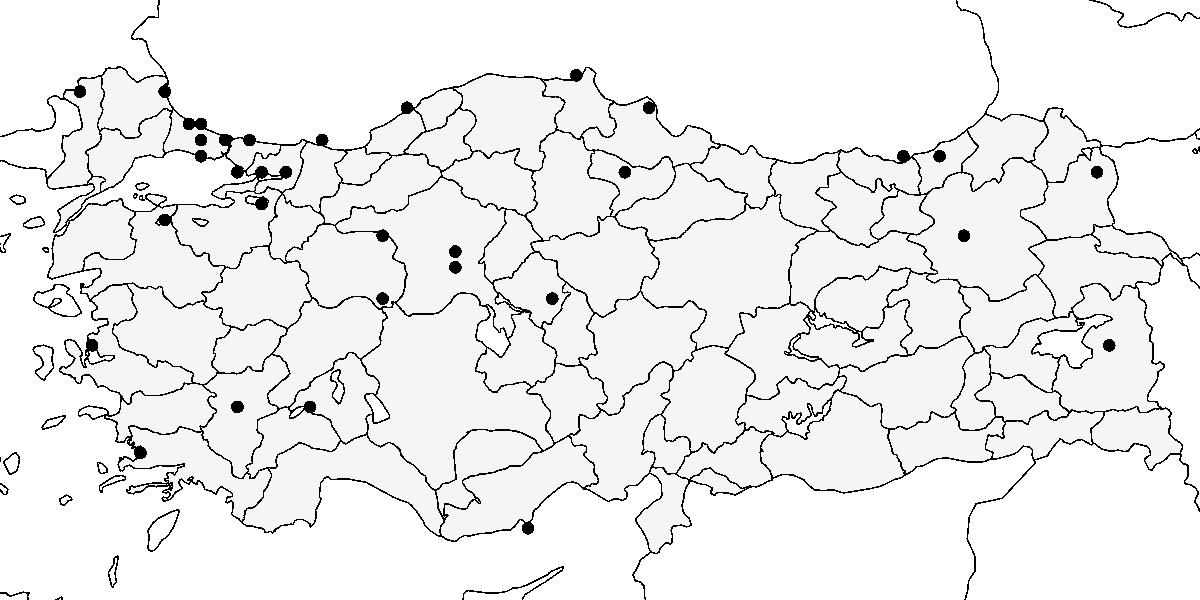
\includegraphics[keepaspectratio]{images/harita_Branta ruficollis.png}}

\textbf{Üreme}

Türkiye'de yuvalamaz. Doğu Sibirya'da tundra kuşağında yuvalar.

\textbf{Alttürler ve Sınıflandırma}

Monotipik bir türdür.

\section{Sessiz Kuğu}\label{sessiz-kuux11fu}

\emph{Cygnus olor}, Mute Swan

\textbf{\emph{Lokal olarak az sayıda yuvalar. Yaygın olarak ve nispeten
çok sayıda bulunan bir kış konuğudur.}}

Üreme kayıtlarının çoğu üç alandan gelir: Gala Gölü, Gediz Deltası ve
Kızılırmak Deltası. Ulusal üreme popülasyonu muhtemelen 20 çiftten daha
azdır. Kızılırmak Deltası'ndan alınan ilk muhtemel üreme kaydı 1968
yılına aittir (Dijksen \& Kasparek, 1985).

Geçmişte, birkaç alanda yüzlerce çiftlik bir üreme nüfusu bulunuyordu.
Marmara Gölü'nde 50 çift, Akşehir Gölü'nde ise 100 çift üremiştir
(Kumerloeve, 1961). Ereğli Sazlığı en çok gözlem kaydının alındığı
alandır. Lenz burada 1968'de 11 yuva, 1969'da bir yuva ve 1970'te üç
yuva bulmuştur. Ereğli Sazlığı'nın yok olması ayrıntılı olarak
belgelenmiştir (Kılıç \& Kasparek, 1990), bu nedenle üreyen nüfusun
azalışı da gözlenmiştir. Eski üreme alanlarında yok olmasının başlıca
nedeni sulakalanların kurutulmasıdır.

Kış aylarında Karadeniz, Marmara ve Ege Bölgelerinde yaygın olarak en
yüksek sayılarda gözlenir. Toplam kışlama popülasyonu 1000-10000 birey
arasında değişmektedir. Meriç Deltası ve Gala Gölü kışlayan nüfusun
büyük kısmının toplandığı alanlardır. 1993'te 1244, 1999'da 8900 ve
2003'te 2000 birey kaydedilmiştir (DHKD, 1993, 1999). Kışın sert geçtiği
yıllarda bu sayı artmakta olup, 1999'da ülke genelinde toplamda 9088
birey kaydedilmiştir.

\pandocbounded{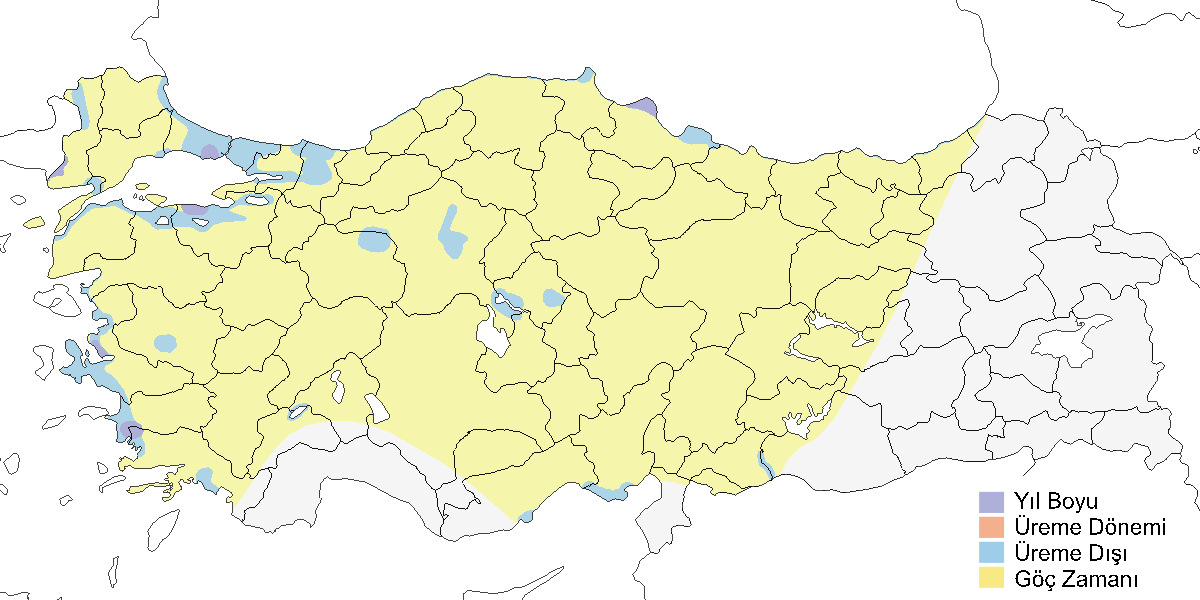
\includegraphics[keepaspectratio]{images/harita_Cygnus olor.png}}

\textbf{Üreme}

\textbf{Yuvalama Alanı:} Geniş sazlık alanlar, su aynası bulunan büyük
göller ve bataklıklarda yuvalar.\\
\textbf{Yuvası:} Türkiye'de henüz bir yuva tarifi yapılmamıştır. Diğer
bölgelerde yuva su kıyısındaki zemin üzerinde, küçük bir adacıkta ya da
sığ sudaki sazların üstüne kurulur. Yuva, saz ve diğer sucul bitkilerden
oluşan büyük bir yığının ortasında çukur şekilli bir yapıdır.\\
\textbf{Yumurta Sayısı:} Türkiye'deki yumurta sayısı bilinmez. Ancak
Türkiye dışındaki yuvalarda genellikle 5-7 yumurta bıraktığı
bilinmektedir.\\
\textbf{Üreme Dönemi:} Nisan başında yumurtlamaya başlar, yavrular ise
mayıs ve temmuz ayları arasında görülür. \textbf{EGE:} 13 Mayıs 1899'da
İzmir'de bir sazlıkta yuvalayan bir çift kaydedilmiştir (Selous, 1900).
\textbf{İÇA:} 6 Temmuz 1976'da Ereğli Sazlığı'nda bir çift ve 4-5 genç
yavru, 17 Temmuz 1982'de bir çift ve dört genç, 16 Mayıs 1987'de ise
yumurtadan yeni çıkmış yavrular gözlenmiştir.

\textbf{Alttürler ve Sınıflandırma}

Monotipik bir türdür.

\section{Küçük Kuğu}\label{kuxfcuxe7uxfck-kuux11fu}

\emph{Cygnus columbianus}, Tundra Swan

\textbf{\emph{Lokal olarak ve az sayıda bulunan bir kış konuğudur.}}

1993 yılına kadar nadir bir kış konuğu olduğu düşünülmüştür. Ancak daha
sonra, önce Burdur Gölü ve Göller Bölgesi'nde, ardından Meriç
Deltası'nda düzenli olarak bulunduğu tespit edilmiştir. Meriç
Deltası'nda, karışık ve kalabalık kuğu sürüleri içinde sayıları 1000'e
kadar ulaşabilir. İç Anadolu ve Göller Bölgesi'nde ise küçük gruplar
halinde bulunur. Genellikle kasım ve nisan ayları arasında gözlenir.

Türkiye'de kışlayan kuşların üreme alanları ve göç koridorları tespit
edilmiştir (Vangeluwe \emph{vd.}, 2018). 2015-2017 yıllarında GPS ve GMS
vericileriyle yapılan çalışmada, yuvalama alanlarının Yamalo-Nenets
Özerk Bölgesi'ndeki Yamal olduğu belirlenmiştir. Göç sırasında Ob Koyu,
Turgay Ovaları, Kuzey Hazar Kıyıları ve Azov Denizi gibi durak alanları
üzerinden göç ettikleri ortaya çıkmıştır.

\pandocbounded{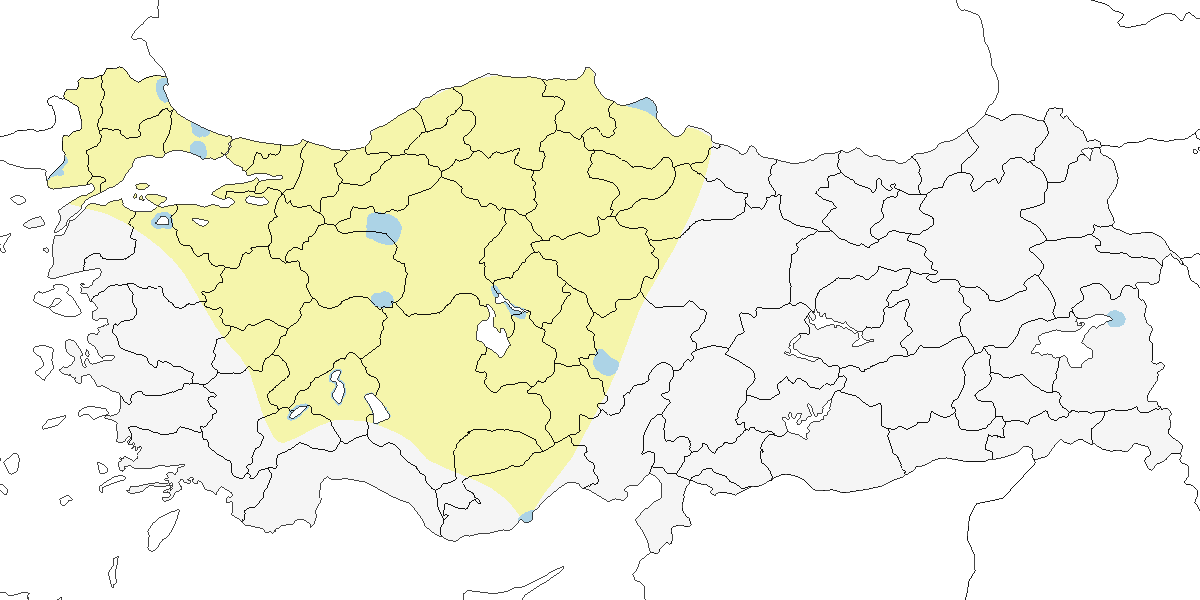
\includegraphics[keepaspectratio]{images/harita_Cygnus columbianus.png}}

\textbf{Üreme}

Türkiye'de yuvalamaz. Sibirya Tundra kuşağında yuvalar.

\textbf{Alttürler ve Sınıflandırma}

Türkiye'de Eski Dünya'da yaşayan \emph{bewickii} alttürü bulunur; bu
alttür, gaga kökü ve yüz derisinin sarı olmasıyla tanınır. Amerika'da
yaşayan \emph{columbianus} alttürü ise siyah gaga ve siyah yüz derisi
ile kolaylıkla ayırt edilebilir.

\section{Ötücü Kuğu}\label{uxf6tuxfccuxfc-kuux11fu}

\emph{Cygnus cygnus}, Whooper Swan

\textbf{\emph{Yaygın olarak ve az sayıda görülen bir kış konuğudur.}}

Ekim sonu ile nisan başı arasında yaygın olarak az sayıda görülen bir
kış konuğudur. Ocak ve şubat aylarında en yüksek sayıya ulaşır.
Trakya'da Meriç Deltası hem Türkiye'deki ana toplama bölgesidir, üstelik
türün Balkanlar'daki en önemli kışlama alanıdır. 25 Ocak 1998'de Meriç
Deltası'nda 1200 birey kaydedilmiş, bu Türkiye'deki en yüksek sayıdır
(Boyla \& Eken, 1998). Türkiye'ye gelen kuşlar, Ukrayna ve Kırım ile
Batı Karadeniz Bölgesi arasındaki deniz üzeri göç rotasını kullanır
(Brazil, 2003). Doğuda, 30 Ekim 1995'te Sodalı Gölü'nde 164 birey
(Adızel, 1998), 1992'de Diyarbakır Kabaklı Barajı'nda 133 birey
kaydedilmiştir (DHKD, 1992).

\pandocbounded{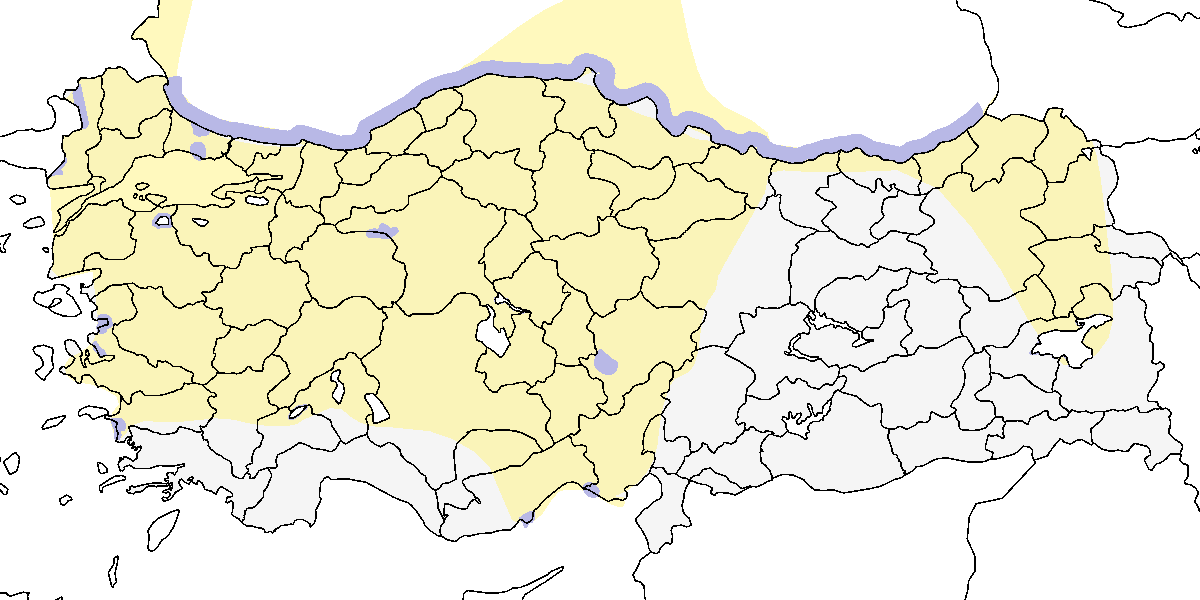
\includegraphics[keepaspectratio]{images/harita_Cygnus cygnus.png}}

\textbf{Üreme}

Türkiye'de yuvalamaz. Üreme bölgesi Kuzey Avrasya'dadır

\textbf{Alttürler ve Sınıflandırma}

Monotipik bir türdür.

\section{Nil Kazı}\label{nil-kazux131}

\emph{Alopochen aegyptiaca}, Egyptian Goose

\textbf{\emph{Durumu belirsizdir. Çoğunlukla egzotik tür kategorisinde
değerlendirilir.}}

28 Nisan 1986'da Kulu Gölü'nde gözlenen bireyin doğal ve rastlantısal
bir konuk olduğu düşünülmüştür. 11 Nisan 1911'de Urfa'nın güneyinde iki
birey gördüğünü söyleyen Weigold'un (1912-13) kaydı kabul edilmemiştir
(Kasparek, 1992a).

İstanbul ve Ankara'da gözlenen kuşların esaretten kaçmış olabileceği
düşünülmektedir. 6-13 Temmuz 2002'de Ankara'daki bir parkta bir çift
fotoğraflanmış; 31 Mart 2012'de İstanbul Riva'da, 13 Mart 2012'de Ankara
Hacettepe Kampüsü'nde, 5-24 Kasım 2013'de Etimesgut'ta ve 25 Mayıs-13
Haziran 2014'te Eymir Gölü'nde birer birey gözlenmiştir.

1906 ve 1928 yılları arasında Kıbrıs'ta nadir görülen bir kış göçmeni
olarak kaydedilmiş ve 1958, 1962 ve 1989 yıllarında bireyler
gözlenmiştir. Eskiden Suriye ve Filistin'de ürediği düşünülmüş (Vaurie,
1965), ancak sonrasında Suriye'de hiçbir güvenilir kaydın olmadığına
karar verilmiştir (Kumerloeve, 1967a; Baumgart, Kasparek \& Stephan,
1995).

\pandocbounded{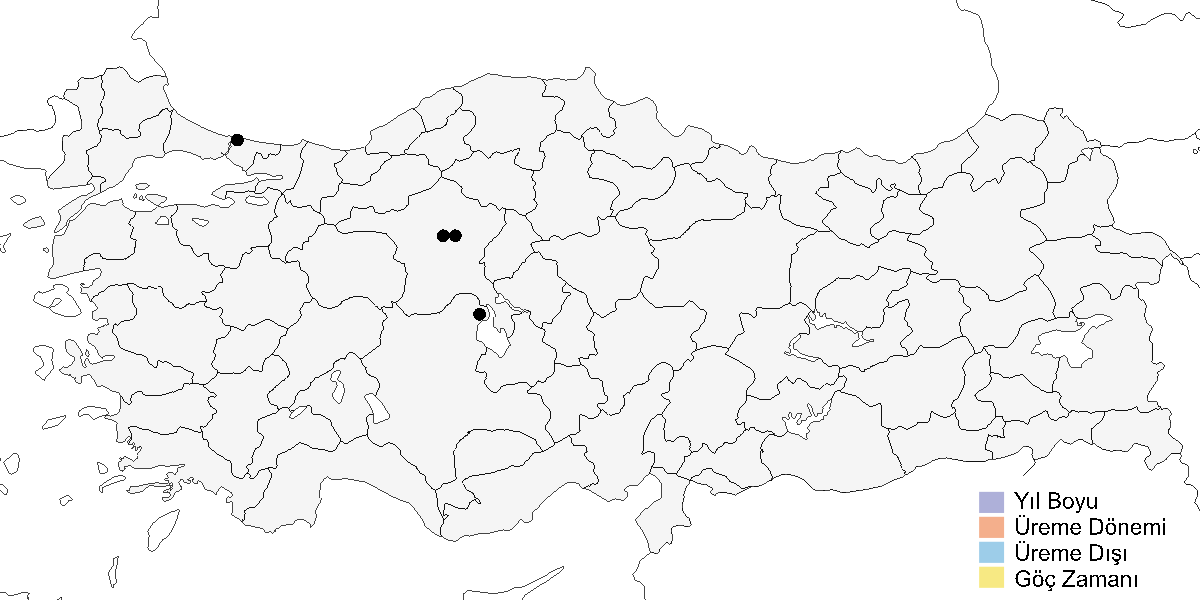
\includegraphics[keepaspectratio]{images/harita_Alopochen aegyptiaca.png}}

\textbf{Üreme}

Türkiye'de yuvalamaz. Üreme alanları çoğunlukla Sahra Altı Afrika'dadır.

\textbf{Alttürler ve Sınıflandırma}

Monotipik bir türdür.

\section{Suna}\label{suna}

\emph{Tadorna tadorna}, Common Shelduck

\textbf{\emph{Lokal olarak az sayıda ürer. Aynı zamanda lokal olarak çok
sayıda bulunabilen bir kış konuğudur.}}

Ege Bölgesi, Göller Bölgesi, İç ve Doğu Anadolu'da geniş ve tuzlu
sulakalanlarda ürer. Başlıca üreme alanları Gediz Deltası, Bolluk Gölü,
Kulu Gölü, Tuz Gölü ve Van Gölü çevresidir. Gediz Deltası'nda 1996
yılında üreyen popülasyonun 8 çift olduğu tahmin edilmiştir (Eken,
1997a). 24 Haziran 1992'de Bolluk Gölü'ndeki bir adada 12 yuva tespit
edilmiştir.

Üreme sonrası tüy değiştiren kuşlar, ağustos ile ekim ayları arasında
toplanır. Bu dönemde Erçek Gölü'nde 2500 birey, Kulu Gölü'nde ise 700
birey sayılmıştır.

Kışlayan toplam nüfus genellikle 1000-5000 birey arasında değişir. Ana
kışlama alanı olan Yumurtalık Lagünü'nde, 16 Şubat 2006'da 5390 birey
kaydedilmiştir. Acıgöl'de ise 1969-70 yıllarında 3450 birey, 1968-69
yıllarında 4900 birey, 2004 yılında 1802 birey ve 2005 yılında 2928
birey sayılmıştır. Diğer alanlarda daha küçük gruplar halinde kışlar.

\pandocbounded{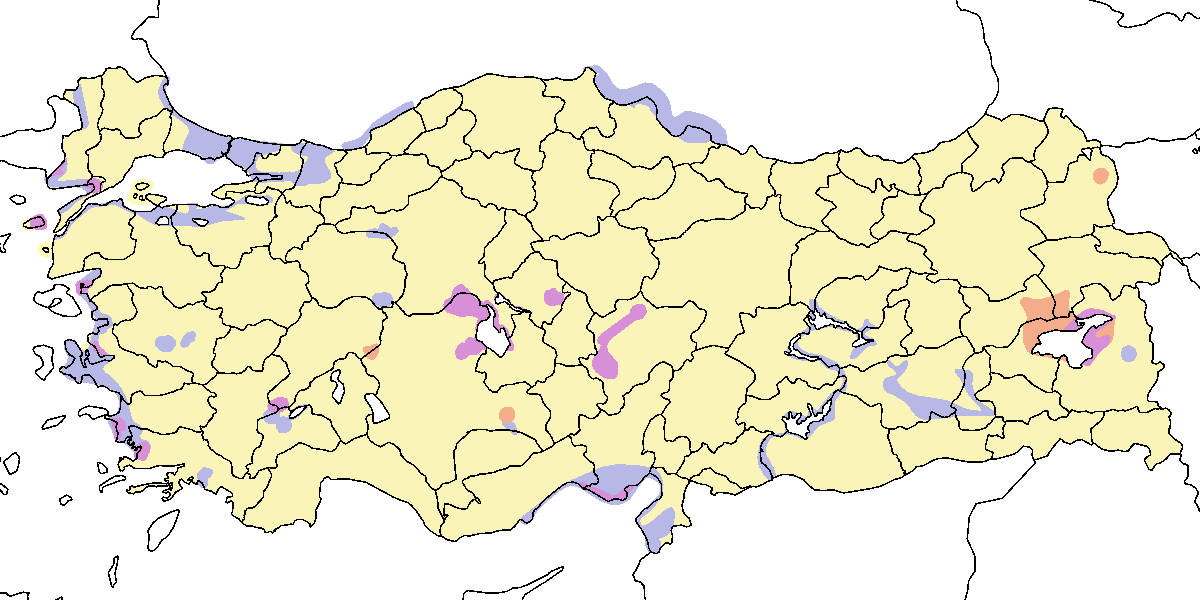
\includegraphics[keepaspectratio]{images/harita_Tadorna tadorna.png}}

\textbf{Üreme}

\textbf{Yuvalama Alanı:} Geniş, sığ ve tuzlu sulakalanlarda, adalar,
sedde duvarları ve çalı altlarında yuvalar.\\
\textbf{Yuvası:} Avrupa'da yuvaların çoğu tavşan oyuklarında, tünelin
1-2 metre içinde bulunur. Ancak Türkiye'deki yuvalar genellikle
yerdedir. Bolluk Gölü'ndeki yuvaların bazıları tamamen açıkta, bazıları
ise kısmen ya da tamamen çalı altında, bir tanesi ise doğal bir oyuğun
içinde bulunmuştur.\\
\textbf{Yumurta Sayısı:} Genellikle 6-9 yumurta bıraktığı gözlenmiştir.
Bolluk Gölü'ndeki yuvalarda gözlenen 10-18 yumurtanın, birden fazla dişi
tarafından bırakılmış olması muhtemeldir.\\
\textbf{Üreme Dönemi:} Gediz Deltası'nda haziran başında yavrular
gözlenmiştir (Eken, 1997a). İç Anadolu'da nisan sonu ile haziran
başında, Doğu Anadolu'da ise haziran ortasında yumurtladığı
düşünülmektedir.

\textbf{Alttürler ve Sınıflandırma}

Monotipik bir türdür.

\section{Angıt}\label{angux131t}

\emph{Tadorna ferruginea}, Ruddy Shelduck

\textbf{\emph{Yaygın ve çok sayıda bulunan yerli türdür. Kışın göç alır,
sayıları artar.}}

Üremek için genellikle yüksek kesimlerdeki küçük gölcükler, baraj
gölleri, ıslak çayırlar ve dereleri tercih eder; birçok ördek ve kaz
türünün aksine büyük sulakalanlarda yuvalamaz. İlk tahminlere göre
üreyen popülasyonun 4000 ile 8000 çift arasında olduğu öne sürülmüştür
(Tucker \& Heath, 1994). Ancak, kış ortası su kuşu sayımlarına dayanarak
popülasyonun azaldığı düşünülmüş ve üreyen popülasyonun 1200-5100 çift
olduğu tahmin edilmiştir (Emirogullari \emph{vd.}, t.y.).

Temmuz ve eylül ayları arasında tüy değişimi için bazı sulakalanlarda
büyük sürüler halinde toplanır. Erçek Gölü'nde 20.000, Sultan
Sazlığı'nda 11.000, Kulu Gölü'nde 10.000 ve Eylül 1936'da, bugün
kurutulmuş olan Emir Gölü'nde 10.000-15.000 birey sayılmıştır. Kış
öncesinde Kasım 2004'te Sarıyar Barajı'nda 8.000 birey ve Kuyucuk
Gölü'nde 6.000 birey kaydedilmiştir.

Kış aylarında daha yaygın olarak görülür. En yüksek kış sayımında
Türkiye genelinde 10.115 birey kaydedilmiş olup (Çağlayan \emph{vd.},
2005), genellikle 4000-4500 birey sayılmıştır. Ocak-Şubat 1993'te sadece
711 birey, 18 Ocak 2004'te Sarıyar Barajı'nda 5636 birey ve 18 Şubat
2006'da 7641 birey kaydedilmiştir. İç Anadolu'da üreme sonrası toplanan
sürülerde bir azalma gözlenirken, baraj göllerinin sayısında artış
olmuştur. Kış sayımı toplamlarının yaz sonu toplamlarından düşük olması,
türün dağınık şekilde kışladığını veya kış aylarında güneye göç ettiğini
göstermektedir. Toplam kışlayan nüfusun 2600 ile 28.500 birey arasında
değiştiği tahmin edilmektedir (Emirogullari \emph{vd.}, t.y.).

\pandocbounded{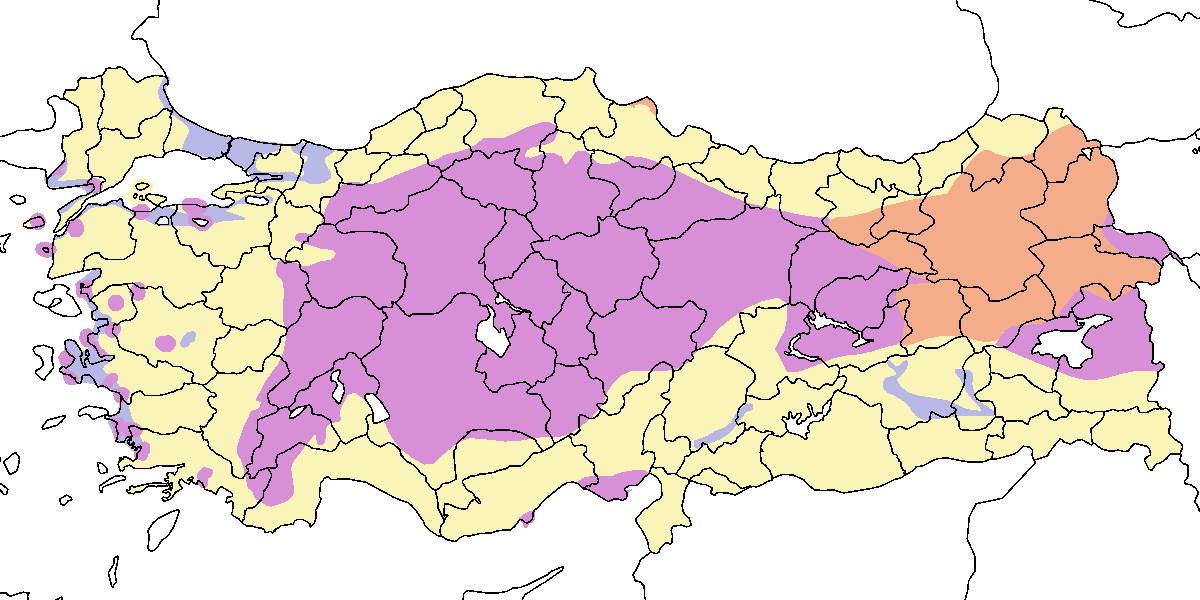
\includegraphics[keepaspectratio]{images/harita_Tadorna ferruginea.png}}

\textbf{Üreme}

\textbf{Yuvalama Alanı:} Genellikle göl kenarındaki sarp kayalıklarda,
tepelerde ve yamaçlardaki çukur ve çatlaklarda, açık alanlarda yuvalar.
Sıkça kayalıklarda yuva yaptığı gözlenmiştir. Beyşehir Gölü'ndeki bir
adada, kayaların ve harabelerin taşları arasında ürediği kaydedilmiştir.
22-24 Mayıs 1998'de Ereğli yakınlarındaki bir kayalıkta, muhtemelen eski
bir Kızıl Şahin yuvasında kuluçkaya yattığı gözlenmiştir.\\
\textbf{Yuvası:} Türkiye'de yuvası bitki artıkları, hav tüyleri ve bazı
diğer tüylerle kaplanmış bir oyuk şeklindedir. 30 Nisan 2003'te Akköy
yakınlarındaki dik bir yamaca giren bir dişi, muhtemelen bir tavşan
yuvası olan bir oyuğa girerken gözlenmiş, ancak oyuğun derin olması
nedeniyle yuva incelenememiştir.\\
\textbf{Yumurta Sayısı:} Genellikle 8-12 yumurta bıraktığı
kaydedilmiştir.\\
\textbf{Üreme Dönemi:} Akdeniz ve Ege bölgelerinde mart sonu yumurtlama
başlar. Diğer bölgelerde kuluçka nisan ve mayıs aylarında gerçekleşir.

\textbf{Alttürler ve Sınıflandırma}

Monotipik bir türdür.

\section{Boz Ördek}\label{boz-uxf6rdek}

\emph{Mareca strepera}, Gadwall

\textbf{Lokal olarak birkaç alanda yuvalar. Yaygın olarak nispeten az
sayılarda görülen bir kış konuğudur.}

Kızılırmak Deltası, bu türün Türkiye'deki en önemli üreme alanıdır ve
yaklaşık 200 çift burada ürer. Türkiye'de toplam üreyen popülasyonun 500
ile 5000 çift arasında olduğu düşünülmüştür (Tucker \& Heath, 1994).
Ancak, günümüzde bu sayının azaldığı açıktır.

İç Anadolu'daki ilkbahar göçü marttan nisan başına kadar belirgin bir
şekilde gözlenir. Akdeniz'deki kıyısal sulakalanlarda ise nadiren
1000'den fazla birey kaydedilir. Kış ortası sayımlarda 1967'de Manyas
Gölü'nde 5000, 1969'da Akşehir Gölü'nde 7500 ve 1971'de Hotamış
Sazlığı'nda 2490 birey sayılmıştır. 1967-1973 yılları arasında ülke
genelinde çoğunlukla 3000'den fazla birey kaydedilirken, 1986-2005
yılları arasında bu sayı 1000-1500 seviyelerine düşmüştür. Son yıllarda
ise yeniden artış göstermiş ve 2020 kışında Kızılırmak Deltası'nda
10.000'den fazla birey sayılmıştır.

\pandocbounded{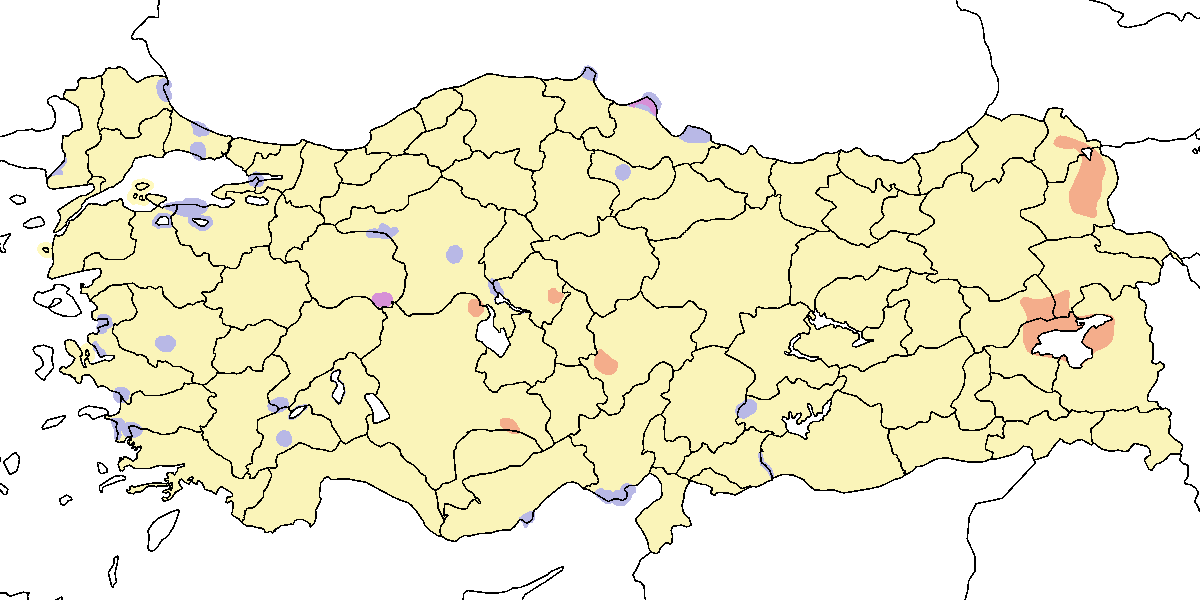
\includegraphics[keepaspectratio]{images/harita_Mareca strepera.png}}

\textbf{Üreme}

\textbf{Yuvalama Alanı:} Göl kıyılarında ve adalarındaki yoğun bitki
örtüsü, sazlıklar ve sık bitkilerle kaplı taşkın alanlarda yuvalar.
Kızılırmak Deltası, Karamık Gölü, Kulu Gölü, Bolluk Gölü, Mogan Gölü,
Ahlat Sazlıkları, Haçlı Gölü ve Van Gölü'nde yuvaladığı gözlenmiştir.\\
\textbf{Yuvası:} Yuva, yerde bir çukura kurulur ve bitkisel malzeme ile
dişinin tüyleriyle kaplanır.\\
\textbf{Yumurta Sayısı:} Türkiye'deki yuvalarda yumurta sayısı 6-15
arasında değişir. İç Anadolu'da 7-15 yumurtalı yuvalar gözlenmiş ve bu
yuvaların bir kısmında 1 ila 6 yumurtanın başka ördek türlerine ait
olduğu tespit edilmiştir. Kulu Gölü'ndeki yuvalarda 6 Mayıs 1972'de 3-11
yumurta ve 14 Temmuz 1971'de 7 yumurta sayılmıştır (Kasparek, 1987a). 17
Mayıs 2004'te Bolluk Gölü'ndeki bir yuvada 8 yumurta bulunmuştur.\\
\textbf{Üreme Dönemi:} Kızılırmak Deltası'nda nisan başında yumurtlamaya
başlar (Hustings \& Dijk, 1994). İç Anadolu'da nisan sonu ile temmuz
arasında, Doğu Anadolu'da ise haziran ile eylül arasında yavrulara
rastlanmıştır.

\textbf{Alttürler ve Sınıflandırma}

Türkiye'de nominat alttür görülür. Tür eskiden \emph{Anas} cinsi altında
sınıflandırılıyordu.

\section{Fiyu}\label{fiyu}

\emph{Mareca penelope}, Eurasian Wigeon

\textbf{\emph{Yaygın olarak çok sayıda bulunan kış konuğu ve geçit
türüdür.}}

Ege, Akdeniz ve İç Anadolu'nun sulakalanlarında kalabalık sürüler
halinde kışlar. 1960'lı ve 1970'li yıllarda düzenli olarak ortalama
150.000 birey sayılmıştır. En yüksek sayılar 1968'de 208.600, 1969'da
ise 458.800 birey olarak kaydedilmiştir. Ancak günümüze gelindiğinde
ciddi bir düşüş yaşanmış, 1986 ile 2005 yılları arasındaki düzenli
sayımlarda yalnızca dört yıl 40.000'den fazla birey kaydedilebilmiştir.
Genellikle eylül sonunda gelir ve nisan sonuna kadar kalır.

İç Anadolu'da mart sonu ve nisan başı arasında yüksek sayılarda göç
eder. Bazı göçmen bireyler mayıs sonuna kadar bölgede kalır. Nadiren de
olsa, İç ve Doğu Anadolu'da üremeden yazı geçiren bireyler gözlenebilir.

\pandocbounded{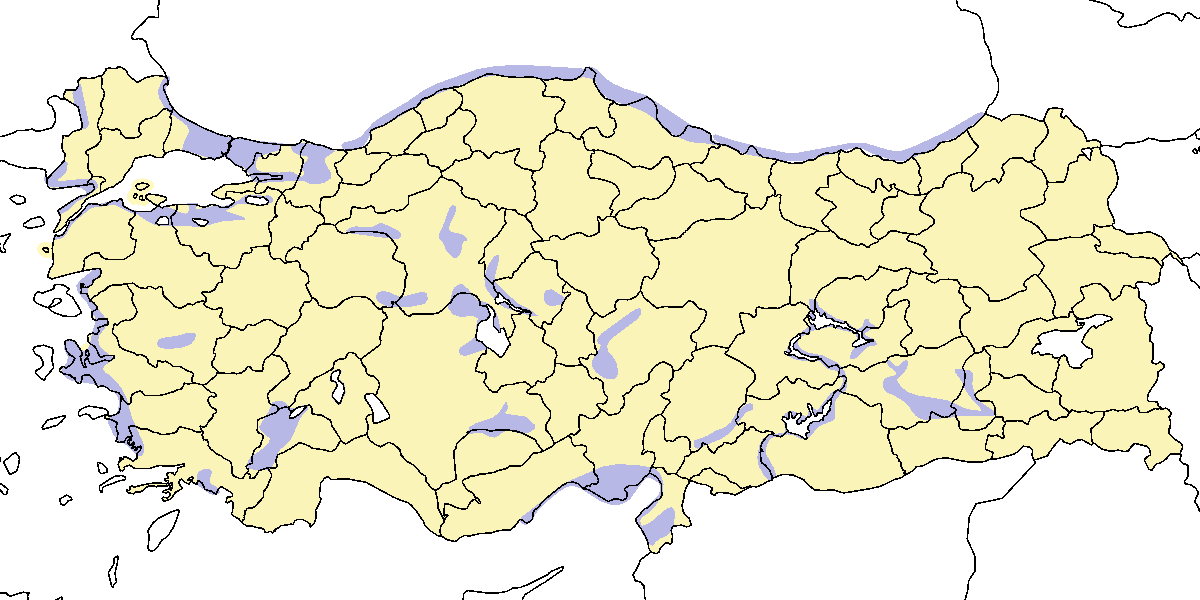
\includegraphics[keepaspectratio]{images/harita_Mareca penelope.png}}

\textbf{Üreme}

Türkiye'de yuvalamaz. Kuzey Avrupa'da yuvalar.

\textbf{Alttürler ve Sınıflandırma}

Monotipik bir türdür. Eskiden \emph{Anas} cinsi altında
sınıflandırılırdı.

\section{Yeşilbaş}\label{yeux15filbaux15f}

\emph{Anas platyrhynchos}, Mallard

\textbf{\emph{Yaygın olarak üreyen yerli bir türdür. Kışın göç alır,
yüksek sayılara ulaşabilir.}}

Uygun yaşam alanlarının bulunduğu bölgelerde az sayıda yuvalar. En
yaygın olarak İç Anadolu Bölgesi'ndeki sulakalanlarda görülür, diğer
bölgelerde ise oldukça lokal bir dağılım gösterir. En yüksek yuvalama
sayısı, 400-600 çiftin kaydedildiği Kızılırmak Deltası'nda olmuştur
(Hustings \& Dijk, 1994).

Sonbaharda göç alır ve popülasyonu artar. Kışlayan gruplar nisan başına
kadar bölgede kalır. En yüksek sayılarda Karadeniz, Marmara ve Ege
bölgelerinde kaydedilirken, Akdeniz ve İç Anadolu'da nispeten az sayıda,
Güneydoğu Anadolu ve Doğu Anadolu'da ise çok daha az sayıda bulunur.
2000 ve 2020 yılları arasında kışlayan nüfus ortalama 20.000 birey
civarındayken, kışın sert geçtiği 2005 yılında Türkiye genelinde toplam
106.140 birey ve Kızılırmak Deltası'nda 50.000 birey sayılmıştır.

1960'lı ve 1970'li yıllarda kışlayan popülasyonun 100.000'ler
seviyesinde olduğu bildirilmiştir. 1967 yılında Kızılırmak ve Yeşilırmak
Deltası'nda yaklaşık 52.000, Büyük Menderes Deltası'nda 42.000; 1968
yılında Manyas ve Uluabat Gölleri'nde 42.000; 1969 yılında Büyük
Menderes Deltası'nda 80.000, Akyatan Lagünü'nde 40.000 ve Amik Gölü'nde
30.000; 1970 yılında ise Meriç Deltası'nda 34.500 ve Sultansazlığı'nda
30.000 birey kaydedilmiştir.

\pandocbounded{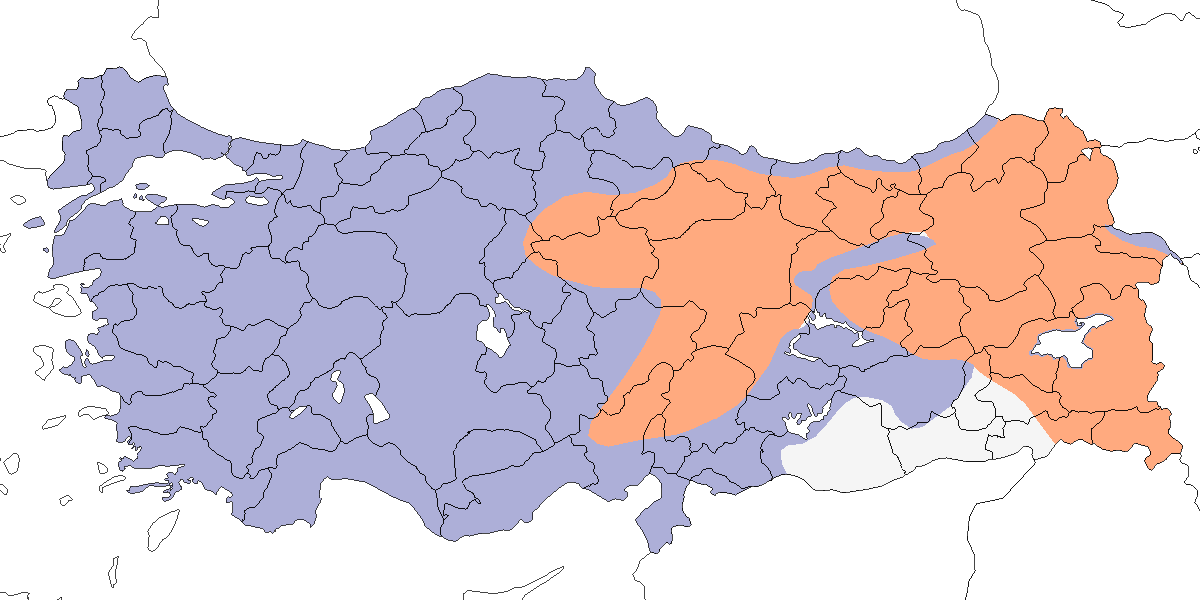
\includegraphics[keepaspectratio]{images/harita_Anas platyrhynchos.png}}

\textbf{Üreme}

\textbf{Yuvalama Alanı:} Göl ve nehir adalarında, sazlıklarda veya göl,
sazlık ve subasar çayırların kıyılarındaki sık bitki örtüsü içinde
yuvalar.\\
\textbf{Yuvası:} Yuvasını genellikle bitki örtüsünün altına, topraktaki
bir oyuğa yapar. Diğer bölgelerde ağaç kovuklarına veya karga gibi
kuşların ağaçlardaki eski yuvalarına yuvaladığı bilinir; ancak
Türkiye'de bu tür yuvalara henüz rastlanmamıştır.\\
\textbf{Yumurta Sayısı:} Genellikle 5-9 yumurta bırakır, ancak yumurta
sayısı 2-14 arasında değişebilir. Bir yuvadaki yumurtaların 14'ten fazla
olması, birden fazla dişinin aynı yuvaya yumurtladığını gösterir.\\
\textbf{Üreme Dönemi:} Kıyı bölgelerinde marttan itibaren, diğer
bölgelerde ise nisan veya mayısta yumurtlar. Yavrular mayıs başından
temmuz sonuna kadar görülebilir. \textbf{MAR:} 18 Nisan 1993'te Kocaçay
Deltası'nda yavrularıyla gözlenen bir dişi, en erken üreme kaydıdır
(Ertan, 1996). \textbf{KAR:} 19-20 Mayıs 1992'de Yeniçağa Gölü'nde
yuvalarda hem yumurta hem yavrular gözlenmiştir. 5 Mayıs 1992'de
Kızılırmak Deltası'nda sezonun ilk yavruları görülmüştür (Hustings \&
Dijk, 1994). 16 Mayıs 1967'de Manyas Gölü'nde dokuz yumurtalı bir yuva
kaydedilmiştir. 20 Haziran 1973'te Trakya'da altı yavrulu bir dişi
gözlenmiştir. \textbf{İÇA:} 1971'de Yarma'daki birçok yuvada diğer
türlerin yumurtalarına rastlanmıştır; örneğin, bir yuvada 17 Yeşilbaş,
üç Boz Ördek ve üç Macar Ördeği yumurtası tanınmıştır. 13-15 Temmuz
1971'de Kulu Gölü'nde sekiz yuva incelenmiş ve yuvalarda 2-12 yumurta
bulunmuştur (Kasparek, 1987a). Başka bir tarihte, mayıs ve haziran
aylarında yumurtalı yuvalar ve mayıs ortasından itibaren yavrular
gözlenmiştir. \textbf{DOA:} En erken kayıt, 14 Haziran 1968'de Erçek
Gölü'nde kaydedilen yavrulardır. Aynı yerde 28 Haziran 1968'de beş ve
sekiz yumurtalı iki yuva bulunmuş, 9 Haziran 2001'de Balık Gölü'nde iki
yumurtalı yuva kaydedilmiştir (Kasparek \& Ven, 1983).

\textbf{Alttürler ve Sınıflandırma}

Türkiye'de nominat alttürü bulunur.

\section{Kaşıkgaga}\label{kaux15fux131kgaga}

\emph{Spatula clypeata}, Northern Shoveler

\textbf{\emph{Lokal olarak az sayıda yuvalar. Aynı zamanda yaygın olarak
çok sayıda bulunan bir geçit türü ve kış konuğudur.}}

İç Anadolu ve Doğu Anadolu'daki birkaç büyük sulakalan ile Kızılırmak
Deltası'nda yuvalar (Boyla, Sinav \& Dizdaroğlu, 2018). 1970'lerde Kulu
Gölü ve Kızılırmak Deltası bilinen üreme alanlarıdır.

Tüm bölgelerde yaygın olarak kaydedilen bir geçit türüdür. Göçmen
gruplar, ilkbaharda mart başından nisan sonuna kadar, sonbaharda ise
eylül ortasından kasım başına kadar zaman zaman yüksek sayılarda
görülür. Eylül ayında Kulu Gölü'nde 7000, Sultansazlığı'nda 9000 ve mart
sonunda Kızılırmak Deltası'nda 4500 birey sayılmıştır.

Ülkenin batı ve orta bölgelerinde kışlar. 2000 ile 2020 yılları arasında
ülke çapında kışlayan kuş sayısı genellikle 5000 bireyin altında
kalmıştır; ancak kışın soğuk geçtiği 2005 yılında 13.576 birey
sayılmıştır. 1990'lı yıllarda daha yüksek sayılar kaydedilirdi; örneğin,
1993'te toplam 7898 birey, 1999'da ise 13.114 birey kaydedilmiştir. Daha
önceki yıllarda yapılan sayımlarda; 1967'de Büyük Menderes Deltası'nda
23.000, Kızılırmak Deltası'nda 8000 birey ve 1993'te 4564 birey
sayılmıştır. 1967-1973 yılları arasında İç Anadolu'daki alanlarda
3000'den fazla bireyden oluşan sürüler olağandı.

\pandocbounded{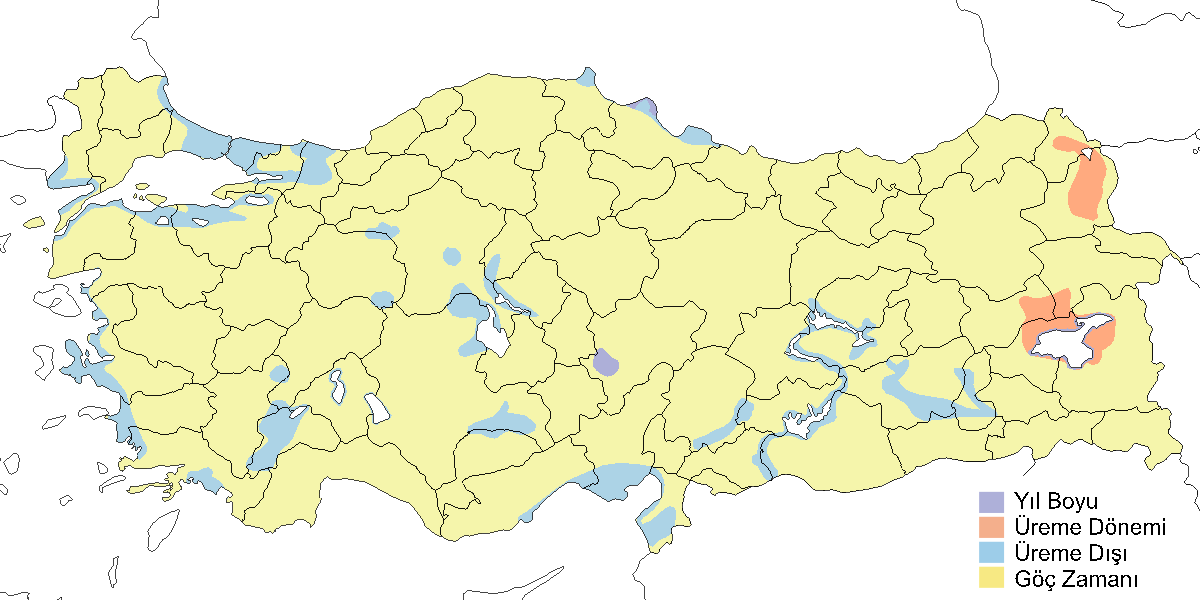
\includegraphics[keepaspectratio]{images/harita_Spatula clypeata.png}}

\textbf{Üreme}

\textbf{Yuvalama alanı:} Büyük sulakalanlarda yuvalar.\\
\textbf{Yuvası:} Kulu Gölü'nde bir adadaki seyrek bitki örtüsü içinde
yuvalamıştır. Yuvasını çıplak zeminde sığ bir oyuk açarak yapar ve içine
ot, bitki gövdeleri ve tüylerini karıştırarak döşer.\\
\textbf{Yumurta sayısı:} 8-10 yumurta bıraktığı kaydedilmiştir.\\
\textbf{Üreme Dönemi:} Türkiye'deki üreme sezonu hakkında yeterli veri
bulunmamaktadır; diğer ülkelerde ise üreme sezonu genellikle nisan başı
ile mayıs sonu arasındadır. \textbf{KAR:} 6-7 Temmuz 1972'de Kızılırmak
Deltası'nda dört ve beş yavrulu iki dişi kaydedilmiştir (Dijksen \&
Kasparek, 1985). 1992 yılında üreme kanıtlanamamış ve popülasyonun 0-1
çift olduğu belirtilmiştir (Hustings \& Dijk, 1994). 1971 yılı Temmuz
ortasında kaydedilen yumurtalı yuvalar, başarısız bir üremenin ardından
gerçekleşen ikinci bir üreme denemesi olarak değerlendirilmiştir.
\textbf{İÇA:} 14-15 Temmuz 1971'de Kulu Gölü'ndeki bir adada sekiz ve on
yumurtalı iki yuva tespit edilmiştir. 5-6 Ağustos 1972'de iki ve dört
yavrulu iki yavru grubu gözlenmiştir (Kasparek, 1987a). 31 Mayıs 1987'de
Kulu Gölü'nde yavrular gözlenmiş, 19 Haziran 1992'de dokuz yumurtalı bir
yuva bulunmuştur. Haziran 1977'de Eşmekaya'da beş yavrusuyla birlikte
bir dişi gözlenmiştir (Schubert, 1979).\\
\textbf{Doğu Anadolu:} 29 Mayıs 1969'da Van Gölü'nde kur davranışı
gözlenmiştir.

\textbf{Alttürler ve Sınıflandırma}

Monotipik bir türdür.

\section{Kılkuyruk}\label{kux131lkuyruk}

\emph{Anas acuta}, Northern Pintail

\textbf{Nispeten yaygın olarak bulunan bir geçit türü ve kış konuğudur.
Nadiren yuvalar.}

Son yıllarda 1998 ve 1999'da, tek bir alanda, Girdev Gölü'nde üremiştir.
İlkbaharda ve yazın İç Anadolu'da birçok erişkin kaydı olsa da,
kanıtlanmış üreme kayıtları az sayıdadır. Üreyen popülasyonun 500 ile
1000 çift olması iddiası tamamen geçersizdir (Tucker \& Heath, 1994).

Genellikle eylül ortasından nisan başına kadar batı ve orta bölgelerde
görülür.

Ülke genelinde kışlayan nüfus 10.000 bireyden azdır. 1986'da toplam
25.700 birey, 1992'de 11.070 birey ve 1999'da 13.573 birey kışlamıştır.
Kışlama popülasyonunda çarpıcı bir azalma belgelenmiştir. 60'li yıllarda
düzenli olarak 100.000'in üzerinde sayılırdı. Örneğin, 1967'de Büyük
Menderes Deltası'nda 60.000 birey, Emir Gölü'nde 70.000 birey, 1969'da
Akyatan Gölü'nde 100.000 birey ve Gâvur Gölü'nde 50.000 birey
kaydedilmiştir. Bilhassa ılıman geçen kışlarda daha yüksek sayılarda
kaydedilebilir. Eski tarihlerde bazı alanlardaki sayımların sonuçlarının
güvenilirliği sorgulanabilir, örneğin, 1970'te Sultansazlığı'ndaki
sayılan 160.000 birey muhtemelen abartılı bir tahmindir. Bu ve diğer
ördek türlerinin önemli sayılarda kışladığı birkaç sulakalan kısmen ya
da tamamen kurutulmuş durumdadır. Diğer yandan son yıllarda oluşan baraj
göllerinde kışlamaya başlamıştır.

\pandocbounded{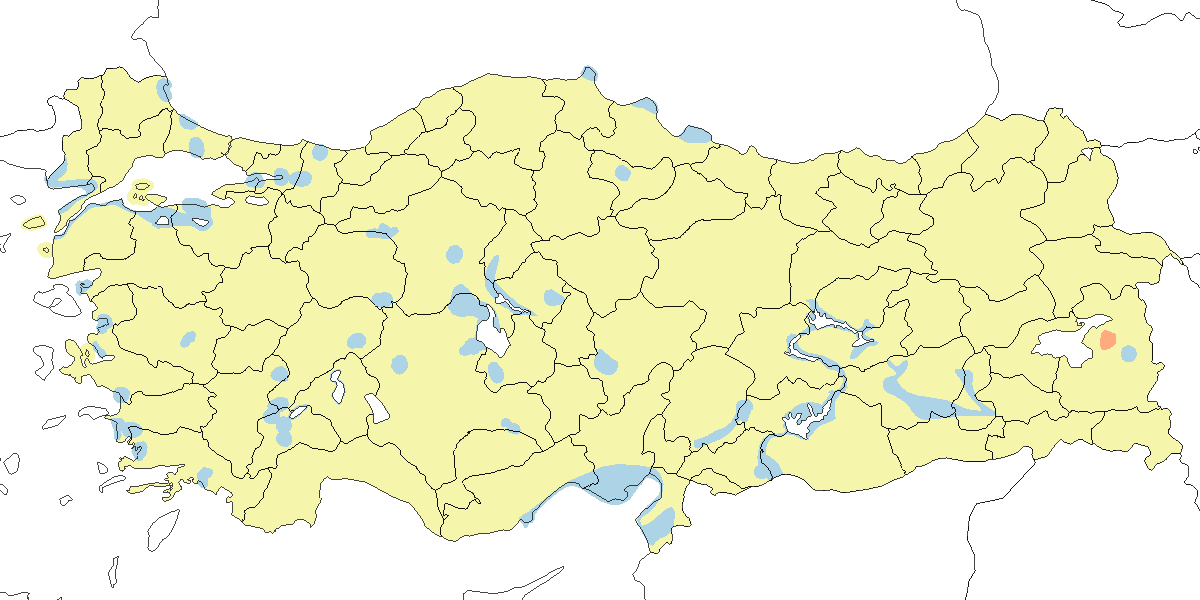
\includegraphics[keepaspectratio]{images/harita_Anas acuta.png}}

\textbf{Üreme}

\textbf{Yuvalama alanı:} Büyük göllerde ve sulakalanlarda yuvalar.\\
\textbf{Yuvası:} Kulu Gölü'ndeki büyük adada kıyı vejetasyonu içinde
yuvalamıştır. Yerdeki bir delikte yaptığı yuvasını bitkisel malzemeler,
hav tüyleri ve kontür tüyleri ile kaplanmıştır.\\
\textbf{Yumurta sayısı:} 6-10 yumurta koyduğu kaydedilmiştir.\\
\textbf{Üreme dönemi:} Görünüşe göre mayıs ayında yumurtlar.
\textbf{KAR:} Kızılırmak Deltası'nda üreme davranışları gözlenmiş,
ürediği kesinleşmemiştir (Hustings \& Dijk, 1994). \textbf{AKD:} Haziran
1998 ve 1999'da Girdev Gölü'nde yavrular gözlenmiştir. \textbf{İÇA:} 22
Mayıs 1992'de Kulu Gölü'nde yedi ve on yumurtalı iki yuva, 19 Haziran
1992'de 6 ila 9 yumurtalı beş yuva bulunmuştur. 24 Haziran 1992'de
Bolluk Gölü'ndeki bir çalının altına gizlenen yuvada 11 yumurta
sayılmıştır.

\textbf{Alttürler ve Sınıflandırma}

Türkiye'de nominat alttürü bulunur.

\section{Çıkrıkçın}\label{uxe7ux131krux131kuxe7ux131n}

\emph{Spatula querquedula}, Garganey

\textbf{Yaygın olarak az sayıda üreyen bir yaz göçmenidir. Bunun yanında
göç döneminde daha yaygın ve çok sayıdadır. Nadiren kışlar.}

Ördeklerin arasında esasen yaz göçmen olan tek türdür. Şubat ortasından
itibaren görülmeye başlar, ekim sonuna kadar kalır. Leylekle beraber en
erken gelen göçmen kuşlardandır. Sazlık sulakalanları tercih eder, en
yoğun ürediği alanlar İç ve Doğu Anadolu'dadır. Güneydoğu Anadolu'da iki
alanda üremesi olasıdır.

İlkbahar ve sonbahar boyunca Türkiye'nin tüm bölgelerinde yüzlerce,
hatta binlerce birey sürüler halinde gözlenebilir. İlkbahar geçişi şubat
sonundan mayıs sonuna kadar devam eder. Sonbahar geçişinde ise ağustos
sonu ile eylül başı arasında Karadeniz kıyıları boyunca göçmen sürülere
rastlanabilir.

Nadiren Marmara, Ege ve Akdeniz'de az sayıda kışlar. Olağandışı yumuşak
geçen 1968-69 kışında Göksu Deltası'nda 3000 birey ve Gâvur Gölü'nde
5000 birey sayılmıştır. Güncel tarihlerde; Ocak 2002'de Güllük
Deltası'nda 65 birey, Şubat 2002'de Bafa Gölü'nde 58 birey, Aralık
2002'de Çukurova'da 89 birey, 4 Aralık 2010'de Karkamış Barajı'nda iki
birey kışlamıştır.

\pandocbounded{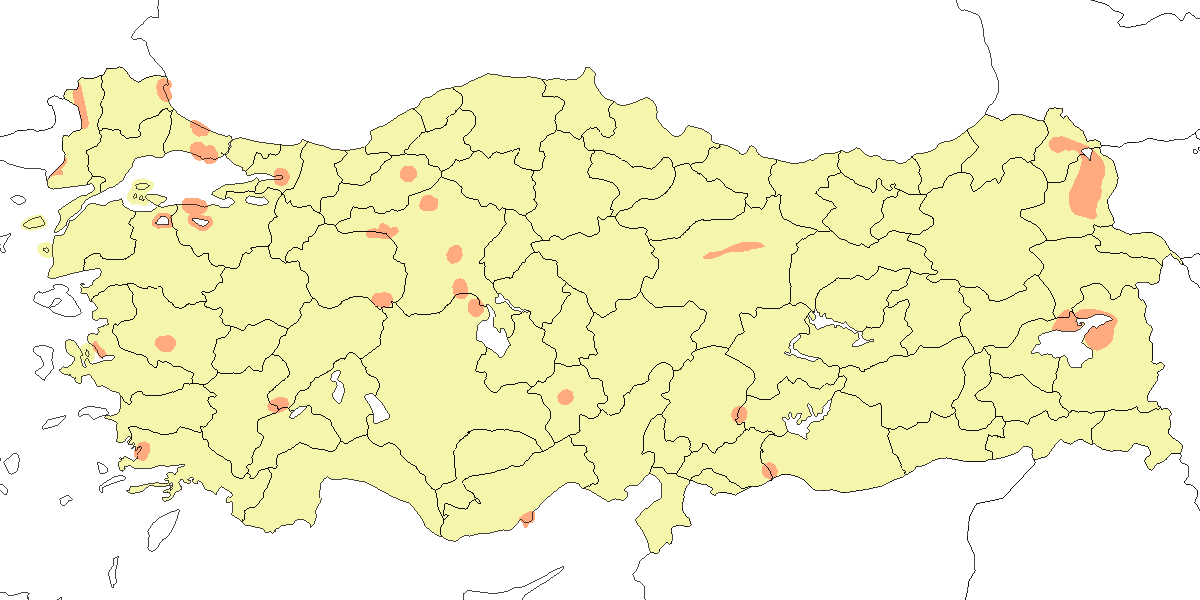
\includegraphics[keepaspectratio]{images/harita_Spatula querquedula.png}}

\textbf{Üreme}

\textbf{Yuvalama alanı:} Sazlık sulakalanlarda yuvalar.\\
\textbf{Yuvası:} Göl kenarlarındaki ıslak çayırlar, bataklıklar ve
sazlıklarda, ikisinin bir arada olduğu alanlarda ve göl kenarındaki
vejetasyonun içinde ürer.\\
\textbf{Yumurta sayısı:} Türkiye'den veri yoktur, diğer yerlerde olağan
yumurta sayısı 8-11'dir.\\
\textbf{Üreme dönemi:} Nisan ortasından itibaren ürer. Yavrular temmuza
kadar görülebilir. \textbf{KAR:} 19 Mayıs 1992'de Yeniçağa Gölü'nde yeni
bozulmuş ancak yumurtaların taze olduğu açıkça anlaşılan iki yuva, 6
Mayıs 1993'te yakınlardaki ıslak bir çayırlıkta bir yuva bulunmuştur. 13
Mayıs 1986'da Abant Gölü'nde 17 yavru ve bir dişi gözlenmiş, yumurtlama
tarihinin nisan ortası civarında olduğunu hesaplanmıştır. 2 Ağustos
1971'de Kızılırmak Deltası'nda bir çift ve yedi yavru kaydedilmiştir.
\textbf{İÇA:} 10-15 Mayıs 1991'de Hotamış Sazlığı'nda yavrulu birkaç
çift gözlenmiş (Kirwan, 1993b), 27 Temmuz 1971'de Kulu Gölü'nde büyük
yavruları olan altı çift kaydedilmiş, Haziran ve Temmuz 1968'de Mogan
Gölü'nde 1-2 kuluçka gözlenmiş, 27 Temmuz 1971'de Yarma'da büyük
yavruları olan en az dört çift tespit edilmiştir.

\textbf{Alttürler ve Sınıflandırma}

Monotipik bir türdür.

\section{Çamurcun}\label{uxe7amurcun}

\emph{Anas crecca}, Eurasian Teal

\textbf{\emph{Lokal olarak az sayıda ürer. Bunun yanında yaygın olarak
ve çok sayıda bulunan kış konuğudur.}}

İç Anadolu, Doğu Anadolu ve Kızılırmak Deltası'nda yuvalar. Kızılırmak
Deltası'nda 1992'de 15-20 çift üremiştir (Hustings \& Dijk, 1994), Doğu
Anadolu'dan teyit edilmiş üreme kaydı ise çok azdır.

Geçiş sırasında eylül başından nisan başına kadar ülkenin batı ve orta
bölgelerinde yaygın olarak çok sayıda görülebilir. Marmara ve Karadeniz
bölgelerinde ara sıra yüksek sayılarda kaydedilebilir.

Kışın hem iç bölgelerde hem de kıyısal sulakalanlarda yüksek sayıda
bulunur. Ülke çapında kışlayan nüfus 100.000 birey seviyesindedir. Son
yıllarda kışlayan nüfusta düşüşler yaşanmış, örneğin 1988'de 21.000
birey ve 1989'da 13.400 birey sayılmıştır. Bu düşüş, aslında diğer yüzey
ördeklerinde olduğu gibi 1960'lardan beri süre gelmektedir. 1968-69'da
toplam 270.400 birey ve 1969-70'te 326.700 birey sayılmıştır. Son
sayımda sadece Sultansazlığı'nda 200.000 birey gözlenmiştir. Alanda
sayılan ancak türü tespit edilemeyen 400.000 ördeğin de çamurcun
olabileceği düşünülürse, alandaki kışlayan çamurcun sayısı 600.000 birey
olabilir.

\pandocbounded{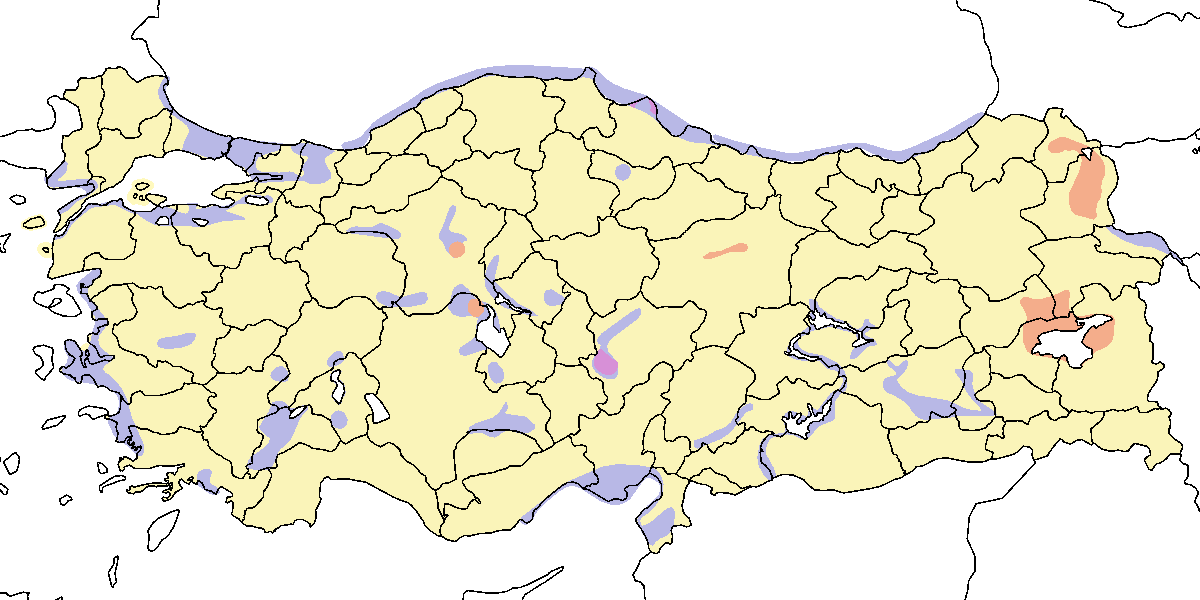
\includegraphics[keepaspectratio]{images/harita_Anas crecca.png}}

\textbf{Üreme}

\textbf{Yuvalama alanı:} Göllerde ve sazlıklarda ürer.\\
\textbf{Yuvası:} Yuva ve yumurta sayısı Türkiye'den bilinmez. Diğer
yerlerde yuvasını yerdeki bir oyuğa yapar ve genellikle yapraklar,
bitkisel malzemeler, hav tüyleri ve kontur tüyleriyle kaplar.
Sulakalanlarda yüksek otların üzerine yuvalar, nadiren sudan uzağa da
yuva yapabilir.\\
\textbf{Yumurta sayısı:} Türkiye'den veri yoktur, ancak diğer yerlerde
olağan yumurta sayısı 8-12'dir.\\
\textbf{Üreme dönemi:} Nisan ortasından itibaren ürer, yavrular temmuza
kadar görülebilir. \textbf{KAR:} 29 Mayıs 1979'da Kızılırmak Deltası'nda
içinde yumurta olan bir yuva bulunmuş, 28 Temmuz 1971'de dokuz yavrulu
bir dişi ve 6 Ağustos 1971'de beş yavrulu bir dişi gözlenmiştir (Dijksen
\& Kasparek, 1985). 1992'de popülasyonun 15-20 çift olduğu belirlenmiş,
5 Mayıs'ta dikkati başka yere çekme davranışı gözlenmiş ancak hiçbir
yuva bulunamamıştır (Hustings \& Dijk, 1994). \textbf{İÇA:} 14 Mayıs
1991'de Hotamış Sazlığı'nda yavrularıyla birlikte birkaç erişkin
gözlenmiş, bu da yumurtaların en geç nisan ortasında koyulmuş olduğunu
göstermiştir (Kirwan, 1993b). 5-6 Ağustos 1972'de Kulu Gölü'nde iki
dişinin 7 ve 10 yavrusu gözlenmiştir (Kasparek, 1987a). \textbf{DOA:} 24
Haziran 1983'te Haçlı Gölü'nde tek yavrulu bir dişi kaydedilmiştir.

\textbf{Alttürler ve Sınıflandırma}

Türkiye'de nominat alttürü bulunur.

\section{Yaz Ördeği}\label{yaz-uxf6rdeux11fi}

\emph{Marmaronetta angustirostris}, Marbled Duck

\textbf{\emph{Türkiye'de üreyen nüfus yok olmuştur.}}

Göksu Deltası'nda üreyen popülasyonun 2013 yılından sonra yok olmasıyla,
üreyen tür olarak Türkiye'deki soyunun tükendiği söylenebilir. Tek tük
Doğu Akdeniz, Güneydoğu ve Doğu Anadolu'da görülebilir. Marmara, Ege ve
Karadeniz bölgelerinde eski tarihli kayıtları vardır. En yakın üreme
alanı Irak'taki Mezopotamya Bataklıkları'dır.

Mart başından ekim başına kadar kaydedilen bir yaz konuğu idi. Göksu
Deltası'ndaki üreyen popülasyon, 1989 ile 2013 arasında adım adım
azalmıştır. 1989 ve 1991'de yaklaşık 50 çift tespit edilmiş, 2000'li
yıllarda bu sayı 10 çifte düşmüş, 2010 ile 2013 arasında sadece 1 ila 2
çift kalmış ve 2014 yılından itibaren alanda görülmemeye başlamıştır. Bu
nedenle Türkiye'de üreyen nüfusunun yok olduğu kabul edilmiş (Boyla
\emph{vd.}, 2018) ve Yaz Ördeği, Yılanboyun'dan sonra Türkiye'de soyu
tükendiği belgelenen ilk kuş türü olmuştur.

1987 yılında Çukurova'da, bugün yok edilmiş olan Dipsiz Gölü'nde 32 çift
tespit edilmiştir. İç Anadolu'da Ereğli Sazlığı'nda muhtemelen 1-4 çift,
Hotamış Sazlığı'nda 10-15 çift ve Sultansazlığı'nda 1-4 çift üremiştir.
Van Gölü havzasında ise Erciş Gölü ve Van Sazlığı'nda az sayıda ürediği
teyit edilmiş, bunun yanında Ağrı çevresi, Ahlat Sazlıkları, Bendimahi
Deltası ve Kuyucuk Gölü'nde üreme döneminde görülmüştür. 1987 yılında
ülke nüfusunun 50-100 çift olduğu düşünülmüştür. Üreme sonrasında
Çukurova ve Göksu Deltası'nda 100-200 bireyin toplandığı bilinir.
Nadiren az sayıda kışlamıştır. En son sayımlarda 1993'te Çukurova'da
dört, 1997'de aynı alanda 35 birey sayılmıştır.

Amik Gölü'nün kurutulmasından önce muhtemelen önemli sayılarda
bulunuyordu (Kumerloeve, 1963a). Konya havzasındaki Yarma Sazlıkları,
Gönenç Gölü ve Karapınar Ovası'nda (Grimmett \& Jones, 1989) muhtemelen
üremiştir. Mogan Gölü ve Eber Gölü gibi diğer birkaç alanda da üremiş
olabilir. Bu alanlar ekolojik özelliklerini kaybettikleri ve türe uygun
üreme habitatları barındırmadıkları için artık üremeye elverişli
değildir. Üreme sonrası toplanan bireyler, o yıllarda toplam ülke nüfusu
hakkında fikir verebilir. Ağustos 1967'de Çukurova'da 2000 birey ve
Göksu Deltası'nda 450 birey sayılmıştır.

\pandocbounded{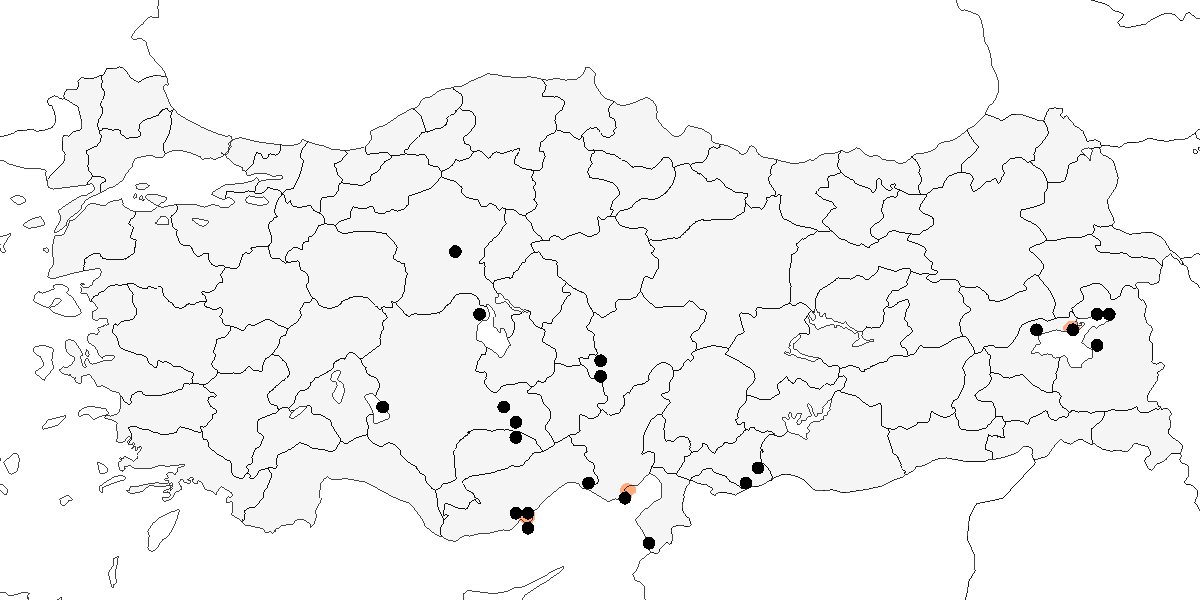
\includegraphics[keepaspectratio]{images/harita_Marmaronetta angustirostris.png}}

\textbf{Üreme}

\textbf{Yuvalama Alanı:} Çukurova ve Göksu Deltası'nda sığ ve ötrofik
göllerde bulunmuştur. Genellikle sazlık adaların, bitişik havuzlar ve
sazlıkların bulunduğu yoğun sualtı vejetasyonuna sahip sığ göllerin
çevresinde ürer ve geniş sulakalanları tercih eder. Sanılanın aksine acı
veya tuzlu sularda değil tatlı suları tercih eder.\\
\textbf{Yuvası:} 9 Haziran 1993'te Göksu'da, kofanın (\emph{Juncus})
baskın olduğu ve yakınlarda sazların (\emph{Phragmites}) da bulunduğu
bataklık bir bölgede sığ gölcüklerin olduğu bir alanda, yaklaşık 1 m
çapındaki bir \emph{Juncus} kümesinin içinde, sudan yaklaşık 0,7 m
yüksekte gizlenmiş iki yumurtalı bir yuva bulunmuştur. Yuva sazlardan ve
bitki gövdelerinden yapılmış dayanıklı bir kâse şeklindedir ve ince
bitkisel malzemeyle kaplanmıştır; hav tüyü kullanılmamıştır.\\
\textbf{Yumurta Sayısı:} Yumurta sayısı 2 ile 12 arasında değişir,
ortalama 6,5 yumurta olarak hesaplanmıştır (Green, 1993). Diğer
bölgelerde ise tipik yumurta sayısı 9-13'tür (5-18).\\
\textbf{Üreme Dönemi:} 22 Mayıs 1971'de Çukurova'da kaydedilen altı
yavru, en erken kayıttır ve yumurtlamanın nisanın ikinci yarısında
başladığını gösterir. Ana yumurtlama dönemi, mayısın ikinci yarısıyla
haziran başı arasındadır. Yavrular en erken 7 Haziran'da ortaya çıkar ve
temmuz sonuna kadar küçük yavrular görülebilir. Tamamen palazlanmış
yavrular temmuz başında kaydedilmiştir. \textbf{AKD:} 1991'de Göksu
Deltası'nda yaklaşık 50 çiftten en az 31'i yavru çıkarmıştır. Aynı yıl
Göksu Deltası'nda 11 yuvada 8-13, 5 yuvada 4-6 ve bir yuvada 15 yavru
sayılmıştır. 15 yavrunun, iki dişinin yumurtalarının bir araya
gelmesiyle oluştuğu düşünülmektedir. Benzer şekilde 15-18 Temmuz 1992'de
bir dişi 32 yavruyla görülmüştür (Green, 1993). 10 Temmuz 1967'de hem
büyük hem küçük yavrular haziran ve temmuzda az sayıda gözlenmiştir
(Vielliard, 1968). \textbf{İÇA:} 4-5 Haziran 1971'de Yarma Sazlığı'nda 6
ve 13 yumurtalı iki yuva bulunmuş, bir yuvada bir Yeşilbaş yumurtası
görülmüştür. 12 Haziran 1998'de Kulu Gölü'nde tek yavrulu bir erişkin
kaydedilmiş ve temmuz ayında üç farklı alanda yavrular gözlenmiştir.
\textbf{DOA:} 22 Temmuz 1987'de Van Sazlığı'nda küçük yavruları olan iki
çift gözlenmiş, bu gözleme dayanarak yumurtlamanın haziran ortasında
olduğu tahmin edilmiştir. Aynı alanda temmuz sonunda ve ağustos başında
genç bireyler kaydedilmiştir.

\textbf{Alttürler ve Sınıflandırma}

Monotipik bir türdür.

\section{Macar Ördeği}\label{macar-uxf6rdeux11fi}

\emph{Netta rufina}, Red-crested Pochard

\textbf{\emph{Lokal olarak nispeten çok sayıda ürer. Kışın daha
yaygındır ve bazı alanlarda yüksek sayılarda toplanır.}}

İç Anadolu'daki geniş sodalı ya da tatlı sazlık sulakalanlarda çok
sayıda ürer. Sultansazlığı'nda yüksek sayılarda bulunur. 1990'larda
Ereğli Sazlığı'nda 500 çift üremişken 1998'de sadece 20 çift üremiş,
alanın kurutulmasıyla buradan tamamen yok olmuştur. Kızılırmak
Deltası'nda 1992'de 50-75 çift üremiştir (Hustings \& Dijk, 1994). Diğer
alanlarda nispeten yüksek sayılarda yuvalayanlar yerli veya yarı
göçmendir. Çukurova sulakalanları ve Göksu Deltası'nda üreyen nüfus
1990'dan sonra azalmıştır. Türkiye'de üreyen popülasyon 1000-5000 çift
olarak tahmin edilmiştir (Tucker \& Heath, 1994). Son yıllarda İç
Anadolu'da üreyen kuşların sayılarında yaşanan azalma, güncel ulusal
nüfusun çok daha az olduğuna işaret etmektedir.

Ülke genelinde geçiş sırasında doğu bölgeleri dışında daha yaygındır.
Çoğu zaman yüzeyi donmaya daha az eğilimli olan baraj göllerini tercih
eder. Ocak 1967'de 12.000 birey sayılmış, bunun 7000'i bugün kurutulmuş
olan Amik Gölü'ndendir. Türkiye genelinde 1992'de 5249, 1996'da 6522 ve
1999'da 6228 birey sayılmıştır. 2000'li yıllarda toplam sayıda artış
görülmüş, sadece Beyşehir Gölü'nde Şubat 2003'te 10.000 birey ve Ocak
2005'te 20.000 birey sayılmış, son sayımda hem toplam hem de alan rekoru
kırılmıştır.

\pandocbounded{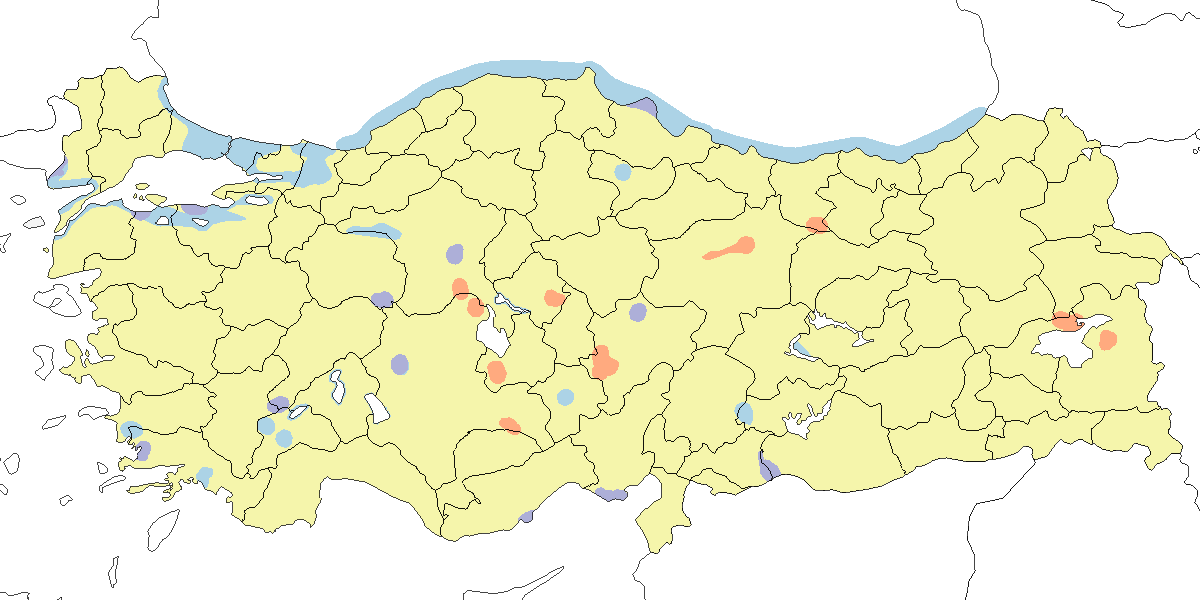
\includegraphics[keepaspectratio]{images/harita_Netta rufina.png}}

\textbf{Üreme}

\textbf{Yuvalama Alanı:} Yoğun sazlıkların ve su kenarı bitkilerinin
bulunduğu tatlı ya da sodalı göllerde ve su aynalarına sahip sazlıklarda
ürer.

\textbf{Yuvası:} Yerdeki bir oyuğa yaptığı yuvasını bitkisel malzeme,
hav tüyleri ve tüylerle kaplar. Çoğunlukla yoğun vejetasyonun içine,
nadiren açıkta (örneğin adalarda) ya da nemli alanlarda su seviyesinin
üzerindeki saz öbeklerinin ya da diğer sucul bitkilerin içine genellikle
iyice gizlenmiş bir yuva yapar.

\textbf{Yumurta Sayısı:} Türkiye'de gözlenen yumurta sayısı 4-12 olup,
ortalama 8,3'tür (18 yuvada). Bir yuvada bulunan 24 yumurta muhtemelen
birden fazla dişiye aittir. Yavru sayısı 2-12 arasında değişir ve 16
yuvada ortalama 6,2'dir. Sadece 2-4 yavru çıkarabilmiş 6 dişi ortalamayı
düşürmüştür.

\textbf{Üreme Dönemi:} Nisan sonu ile temmuz başı arasında yumurtlar.
Yavrular temmuz sonuna kadar görülebilir. \textbf{MAR:} 1 Mayıs 1993'te
Kocaçay Deltası'nda yumurtalı bir yuva bulunmuştur (Ertan, 1996).
\textbf{KAR:} Kızılırmak Deltası'nda 27 Mayıs 1992'de beş yumurtalı bir
yuva bulunmuş, 4 Haziran 1992'de yaklaşık bir haftalık ilk tüylü yavru
kaydedilmiş (Hustings \& Dijk, 1994) ve 27 Mayıs 1979'da sekiz yavrulu
bir aile gözlenmiştir (Dijksen \& Kasparek, 1985). \textbf{AKD:} 18
Temmuz 1992'de Karamık Gölü'nde küçük yavrulardan oluşan bir aile
gözlenmiştir. \textbf{İÇA:} Çoğu mayısta olmak üzere 25 Nisan'da yumurta
kayıtları vardır. En geç kayıt 19 Haziran 1992'de 12 yumurtalı bir
yuvadır. Biri 11 Mayıs'ta, çoğu haziranda olan birçok yavru kaydı
vardır, en geç 8 Temmuz 1967'de (Vielliard, 1968) ve 5 Ağustos 1972'de
küçük yavrular gözlenmiştir. \textbf{DOA:} 21-22 Temmuz 1986'da Van
Gölü'nde 7-8 yavrulu üç yavrulu bir aile kaydedilmiştir.

\textbf{Alttürler ve Sınıflandırma}

Monotipik bir türdür.

\section{Elmabaş Patka}\label{elmabaux15f-patka}

\emph{Aythya ferina}, Common Pochard

\textbf{Nispeten yaygın ve çok sayıda bulunan yerli ve yarı göçmen,
yaygın ve çok sayıda bulunan kış konuğudur.}

İç ve Doğu Anadolu'daki sulakalanlarda orta sayılarda üreyen yerli ve
yarı göçmendir. 1992'de Kızılırmak Deltası'nda 300-350 çiftin ürediği
tahmin edilmiştir (Hustings \& Dijk, 1994). Uygun habitatların azlığı
nedeniyle Karadeniz, Güneydoğu Anadolu ve diğer bölgelerde lokal olarak
bulunur. Muhtemelen gerçek üreme durumunu çarpıtacak şekilde, hatırı
sayılır sayıda üremeyen birey özellikle İç ve Doğu Anadolu'da yazı
geçirir.

Kışın ve geçiş dönemlerinde ülke genelinde yaygın ve boldur. Son
yıllarda ortalama 67.000 bireyden fazla sayılmaktadır. 1996 yılında
Beyşehir Gölü'nde 47.000, Uluabat Gölü'nde 42.000 ve ülke genelinde
toplamda 250.000 birey sayılmıştır, bu en yüksek kayıtlardandır. 1999'da
Eğirdir Gölü'nde 40.000, ülke genelinde ise 137.000 kuş sayılmıştır. 18
yıllık Kış Ortası Su kuşu sayımlarının ortalaması 93.000 kuştur. İstisna
olarak 1968-69 kışında 355.000 bireyin kışladığı tahmin edilmiştir. Ekim
ortasından itibaren yüksek sayılar gözlemlenir; Göksu Deltası'nda Ekim
1978'de 40.000, Ekim 2002'de Sodalıgöl'de 100-130.000, Kulu Gölü'nde
Kasım 1970'te 45.000 ve Kasım 1971'de 28.000 birey kaydedilmiştir.

\pandocbounded{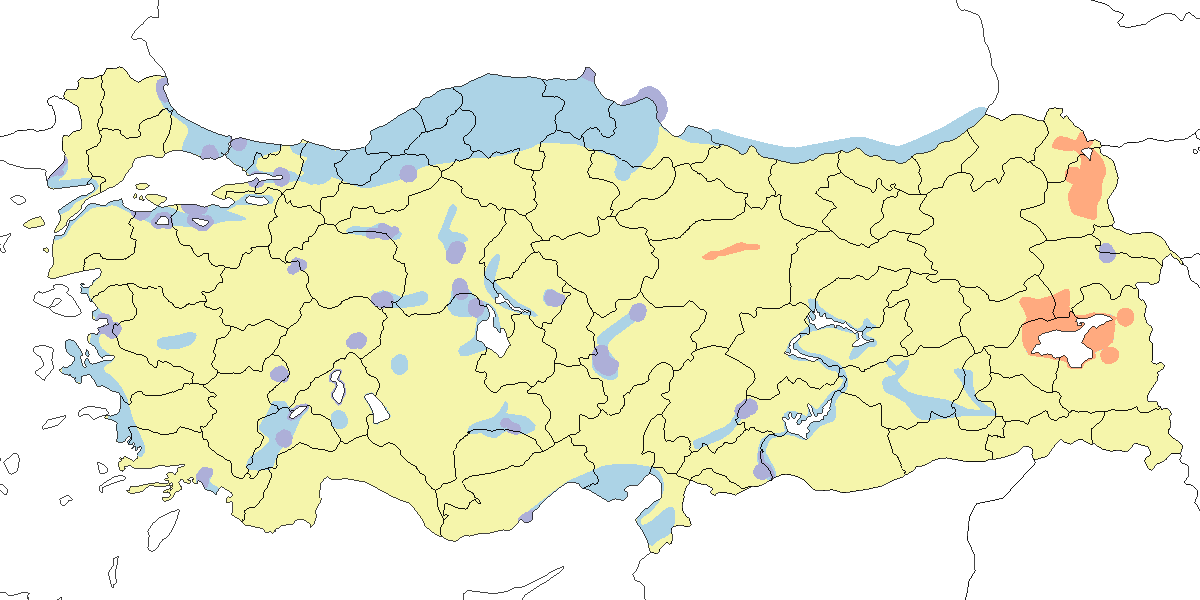
\includegraphics[keepaspectratio]{images/harita_Aythya ferina.png}}

\textbf{Üreme}

\textbf{Yuvalama alanı:} Göl kıyılarındaki sazlıklarda ve su aynalarının
bulunduğu sazlık bataklıklarda ürer.\\
\textbf{Yuvası:} 19 Haziran 1984'te Erçek Gölü yakınlarındaki küçük bir
gölde, sık bir örtü içindeki sazların dibine tutturulmuş ve sakarmeke
yuvasına benzer şekilde sudan yükseğe yapılmış bir yuva bulunmuştur.
Yuva, ölü saz gövdeleri ve diğer bitkisel malzemelerle derin ve düzgün
bir kâse şeklinde örülmüş, bol miktarda hav tüyü ve diğer tüylerle
kaplanmış dayanıklı bir yapıya sahiptir. Diğer bölgelerdeki yuvalar da
genellikle benzer alanlarda olup nadiren su kıyısındaki yoğun bitki
örtüsünün içinde kuru zeminde de bulunabilir.\\
\textbf{Yumurta Sayısı:} Türkiye'de yumurta sayısı kaydedilmemiştir,
ancak gözlenen yavru sayısından 8-11 yumurta bırakabileceği
düşünülmektedir. Diğer bölgelerde genellikle 6-9 yumurta bırakır.
Gözlenen yavru sayısı ortalama 6,6'dır.\\
\textbf{Üreme Dönemi:} Nisan başı ile haziran ortasına kadar yumurta
bırakır. Yavrular temmuz ayında gözlenebilir. \textbf{KAR}. Kızılırmak
Deltası'nda 11 Mayıs 1992'de hav tüyleriyle kaplı birkaç günlük yavru,
en erken kayıt olarak görülmüş ve bu da yumurtlamanın nisanın ilk
haftasında olduğunu göstermiştir (Hustings \& Dijk, 1994). 14 Haziran
1984'te yaklaşık 5 günlük yavrulardan oluşan bir kuluçka ile yaklaşık üç
haftalık yavrulardan oluşan iki kuluçka gözlenmiştir (Dijksen \&
Kasparek, 1985). \textbf{İÇA}. Haziran başlarında iki yumurtalı
(tamamlanmamış) bir yuva bulunmuş, Haziran 1971'de Boz Ördek yuvalarına
iki, dört ve beş yumurta bırakıldığı tespit edilmiştir. 13 Mayıs 1991'de
Hotamış'ta yumurtalı bir yuva bulunmuştur (Kirwan, 1993b). 1970 yılının
mayıs ayı sonunda Eşmekaya'da küçük yavrulardan oluşan beş yavru, 1
Haziran 1969'da Sultansazlığı'nda altı yavru ve haziran-temmuz aylarında
diğer alanlarda yavrular gözlenmiştir. \textbf{DOA}. 19 Haziran 1983'te
Van Sazlığı'nda yavrularıyla birlikte sekiz dişi kaydedilmiştir.

\textbf{Alttürler ve Sınıflandırma}

Monotipik bir türdür.

\section{Pasbaş Patka}\label{pasbaux15f-patka}

\emph{Aythya nyroca}, Ferruginous Duck

\textbf{Lokal olarak az sayıda üreyen yaz konuğu, yaygın ve nispeten çok
sayıda bulunan geçit türü, yaygın ancak az sayıda kış konuğudur.}

Tüm bölgelerdeki sulakalanlarda oldukça lokal bir yaz konuğudur. En
yüksek sayılarda İç ve Doğu Anadolu bölgelerinde bulunur. Kızılırmak
Deltası (1992'de tahminen 150-200 çift (Hustings \& Dijk, 1994), Kocaçay
Deltası (1993'te tahminen 70 çift (Ertan, 1996), Uluabat Gölü (1988'de
tahminen 32 çift (Welch \& Welch, 1998b) ve Göksu Deltası (yaklaşık 30
çift) önemli sayılarda ürediği alanlardır. Son yıllarda gerçekleştirilen
çalışmalarda Güneydoğu Anadolu'da üç yeni üreme alanı belirlenmiştir.
Yaz göçmenleri mart ortasından eylül sonuna kadar gözlenir.

Türkiye popülasyonu muhtemelen dünyadaki en önemlilerinden biridir ve
1000 ile 3000 çift arasında olduğu düşünülmüş (Tucker \& Heath, 1994),
sonra bu tahmin 500-600 çift olarak güncellenmiştir (Kirwan, 1997a).
Avrupa'da yayılış alanının bir kısmında yaşanan sert düşüş dikkate
alındığında, Türkiye popülasyonunun izlenmesine acil ihtiyaç
duyulmaktadır. 1990'ların sonlarında İç Anadolu'daki birkaç alanda da
azalma görülmüştür.

Geçiş sırasında az ve orta sayılarda bulunur ve ülke genelinde biraz
daha yaygındır. Az sayıda kışlar, 1992 yılında 105 birey, diğer yıllarda
50 bireyden az sayılmıştır. 1990'ların ortalarından itibaren kış
kayıtlarında bir artış gözlenmiş, bu durum muhtemelen gözlemci sayısının
artmasına bağlanmıştır. Eskiden batı ve orta bölgelerde daha çok sayıda
kışlamış, 1968-74 yıllarında 50 ile 450 birey arasında kaydedilmiştir.
Marmara Gölü'nde kaydedilen 860 birey en yüksek kayıttır. Doğu ve
Güneydoğu Anadolu'da 2005 yılında sayılan 44 birey bahsedilmeye
değerdir.

\pandocbounded{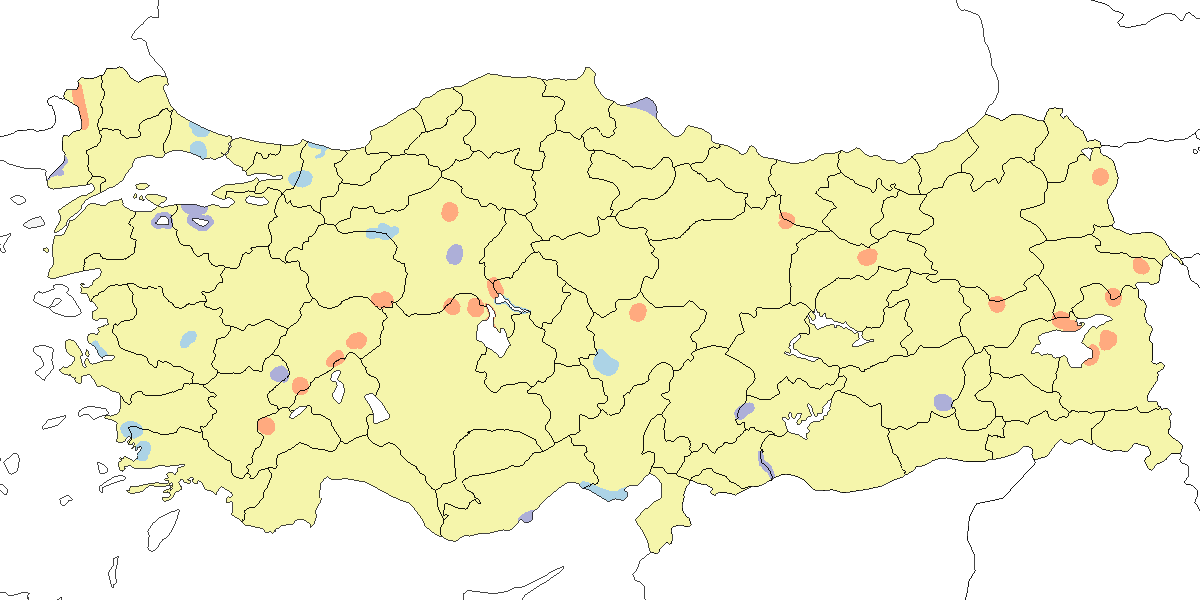
\includegraphics[keepaspectratio]{images/harita_Aythya nyroca.png}}

\textbf{Üreme}

\textbf{Yuvalama Alanı:} Çevresinde sazlıkların, yoğun su üstü
vejetasyonunun ve çoğunlukla daha geniş sazlıkların ve bataklıkların
bulunduğu tatlı su göllerinde ürer.\\
\textbf{Yuvası:} Su kenarındaki yoğun vejetasyonun içine yuva yapar.
Kulu Gölü'ndeki bir adada, alçak çalıların arasında çıplak zeminde hafif
bir çukurun içine yapılan yuvanın ot ve hav tüyleriyle kaplandığı
gözlenmiştir (Pforr \& Limbrunner, 1982); A. Limbrunner, kişisel
görüşme).\\
\textbf{Yumurta Sayısı:} Türkiye'de gözlenen yumurta sayısı 6-8
arasındadır.\\
\textbf{Üreme Dönemi:} Nisan ile haziran başı arasında yumurta bırakır.
Yavrular ağustos ayına kadar gözlenebilir. \textbf{MAR:} 19 Haziran
1999'da Uluabat Gölü'nde bazıları küçük yavrulardan oluşan birkaç yavru
grubu gözlenmiş, 1966'da Manyas Gölü'nde de yavrular kaydedilmiştir.
\textbf{KAR:} Kızılırmak Deltası'nda çiftlerin çoğu sazlık alanlarda
gözlenmiştir. 5 Mayıs 1992'de altı yumurtalı bir yuva bulunmuş ve 1
Haziran 1992'de yumurtlamanın nisan sonlarından daha geç olmadığını
gösteren üç ve dört yavrulu iki grup kaydedilmiştir (Hustings \& Dijk,
1994). 6 Ağustos 1971'de yedi yavrulu bir grup gözlenmiştir.
\textbf{AKD:} 15 Mayıs 1962'de Çukurova'da sekiz yumurtalı bir yuva
(Kirwan, 1997a), 8 Mayıs 1953'te Amik Gölü'nde yumurtalı bir yuva
(Kirwan, 1997a), ve 27 Mayıs 1933'te yumurta kanalında yumurta bulunan
bir dişi vurulmuştur (Meinertzhagen, 1935). Göksu Deltası'nda en erken
17 Haziran'da olmak üzere yedi yuva alanında yavrular gözlenmiştir.
\textbf{İÇA:} 28 Nisan 1982'de Sultansazlığı'nda yumurtalı bir yuva
bulunmuştur (Kirwan, 1997a). Mayıs 1973'te Kulu Gölü'nde altı yumurtalı
bir yuva bulunmuştur. En erken 20 Haziran'da Eber Gölü'nde olmak üzere
Çöl Gölü, Gönenç Gölü, Sultansazlığı, Mogan Gölü ve Kulu Gölü'nde
yavrular gözlenmiştir. \textbf{DOA:} Yumurtlamanın mayıs sonunda
olduğunu gösteren gözlemler 1985 ve 1987 yıllarında haziran sonunda Van
Gölü'nde ve 29 Haziran 1987'de Edremit Sazlığı'nda yapılmıştır (Kirwan,
1997a).

\textbf{Alttürler ve Sınıflandırma}

Monotipik bir türdür.

\section{Tepeli Patka}\label{tepeli-patka}

\emph{Aythya fuligula}, Tufted Duck

\textbf{\emph{Lokal ve az sayıda üreyen yaz konuğu, nispeten yaygın ve
çok sayıda bulunan kış konuğudur.}}

Çok nadir ve lokal olarak üremiştir. Kızılırmak Deltası'nda ve 1967 ile
1981'de Çalı Gölü'nde (Kars) ürediği kanıtlanmış, son alanda 20 çiftlik
bir popülasyon tespit edilmiştir. Başka bölgelerde düzenli olarak yazı
geçirir. Uluabat Gölü ve Uyuz Gölü gibi bazı alanlardaki uygun
habitatlarda çiftler gözlenmiştir. Üreme sonrasında, Temmuz 1982'de Kulu
Gölü'nde tüy değişimi için toplandıkları düşünülen 700 birey (Kasparek,
1987a), Eylül 1967'de ise Sodalı Gölü'nde çoğu erkek olan 1200 birey
sayılmıştır.

Ülkenin batı ve orta bölgelerinde eylül başından nisan başına kadar
kaydedilen yaygın ve bol bulunan bir geçiş türü ve kış konuğudur.
Karadeniz'de denizde kışlar. Kış ortası sayımlarında; 1968-69 kışında
20.800 birey, 1996'da en yüksek sayı olan 58.271 birey, 1992'de yaklaşık
13.000 birey, 1993'te 16.965 birey (sadece Eğirdir Gölü'nde 10.478
birey) ve 1999'da 18.512 birey kaydedilmiştir. Son yıllarda ise ülke
toplamı genellikle 5000-10.000 birey arasındadır. En önemli kışlama
alanları Sapanca Gölü ve Eğirdir Gölü'dür.

\pandocbounded{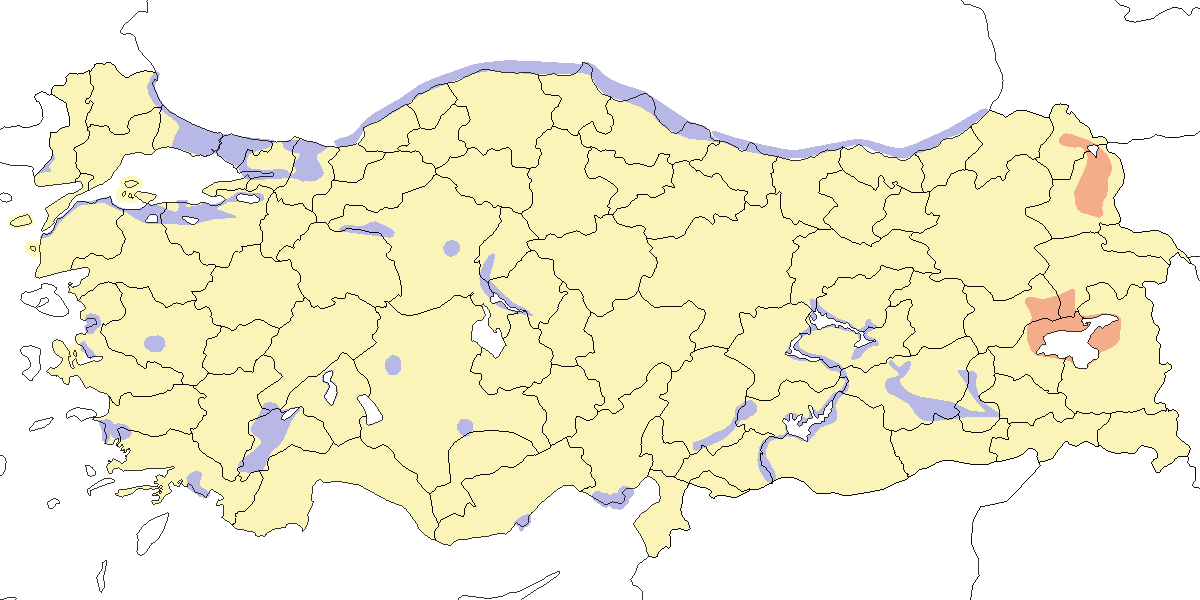
\includegraphics[keepaspectratio]{images/harita_Aythya fuligula.png}}

\textbf{Üreme}

\textbf{Yuvalama alanı:} Su üstü vejetasyonu olan tatlı su göllerinde
ürer.\\
\textbf{Yuvası:} Yuvasını bir bitki öbeğinin altına kurar.\\
\textbf{Yumurta sayısı:} Türkiye'de 8 yumurtalı bir yuva bulunmuştur.\\
\textbf{Üreme dönemi:} Mayıs ayında yumurta koyar, temmuz sonuna kadar
yavrular görülebilir. \textbf{KAR:} Kızılırmak Deltası'nda, 5 Mayıs
1992'de sazlıkta bir \emph{Juncus acutus} öbeğinin dibinde sekiz
yumurtalı bir yuva bulunmuş (Hustings \& Dijk, 1994) ve 28 Mayıs 1968'de
de ürediği kanıtlanmıştır (Dijksen \& Kasparek, 1985). \textbf{DOA:}
Çalı Gölü'nde 19 Temmuz 1992'de yavrularıyla birlikte iki dişi
gözlenmiştir (Magnin \& Yarar, 1997).

\textbf{Alttürler ve Sınıflandırma}

Monotipik bir türdür.

\section{Karabaş Patka}\label{karabaux15f-patka}

\emph{Aythya marila}, Greater Scaup

\textbf{\emph{Özellikle Karadeniz kıyılarında az sayıda ve düzenli
olarak görülen kış konuğudur.}}

Karadeniz ve Marmara Bölgesi'nde hemen hemen her yıl az sayıda
görülmektedir. Modern kuş tayininin başlaması sonrasında gelen kayıtlar
şöyledir (OST, 1969, 1972, 1975, 1978): Ocak-Şubat 1969'da Sakarya
Deltası'nda yedi birey, Manyas ya da Uluabat Gölü'nde dört birey
görülmüştür. Kızılırmak Deltası'ndaki Liman Gölü'nde 1990'ların
başlarında kışlayan 38 birey, 1970'lerde aynı alandan bildirilen şüpheli
kayıtların (Dijksen \& Kasparek, 1985) geçerli olabileceğini düşündürür.

Çoğu İstanbul civarından olan geçmiş veriler şöyledir: Şubat 1893'te
Çekmece'de daha çok dişi ve gençlerden oluşan bir grup gözlenmiş ve şu
anda Sofya Doğa Tarihi Müzesi'nde bulunan erkek örnek toplanmıştır
(Alléon, 1880). İstanbul Robert Kolej'de bulunan dişi örnek
(Mathey-Dupraz, 1920--24), 1998'deki bir ziyarette bulunamamıştır
(Kirwan, 1997b). 1946-47 ve 1947-48 kışlarında Çatalağzı açıklarında
(Zonguldak) belirsiz sayıda gözlenmiş (Ogilvie, 1954), 15 Ocak 1950'de
bilinmeyen bir yerden altı örnek alınmıştır (Kumerloeve, 1970a).
Büyükçekmece'de Ocak 1963'te bir erkek ve Şubat 1964'te bir dişi
kaydedilmiştir (Kumerloeve, 1970a).

Türün ilk yaz kaydı 30 Mayıs 1992'de Sodalı Gölü'nde kaydedilen iki
erkektir (Kirwan \& Martins, 1994). Öte yandan, 19 Nisan 1981'de Kulu
Gölü'nde gözlenen iki birey, 12 Nisan 1990'da Göksu Deltası'nda gözlenen
yaklaşık 20 birey (Kirwan \& Martins, 2000) olağandışı geç kayıtlardır.

\pandocbounded{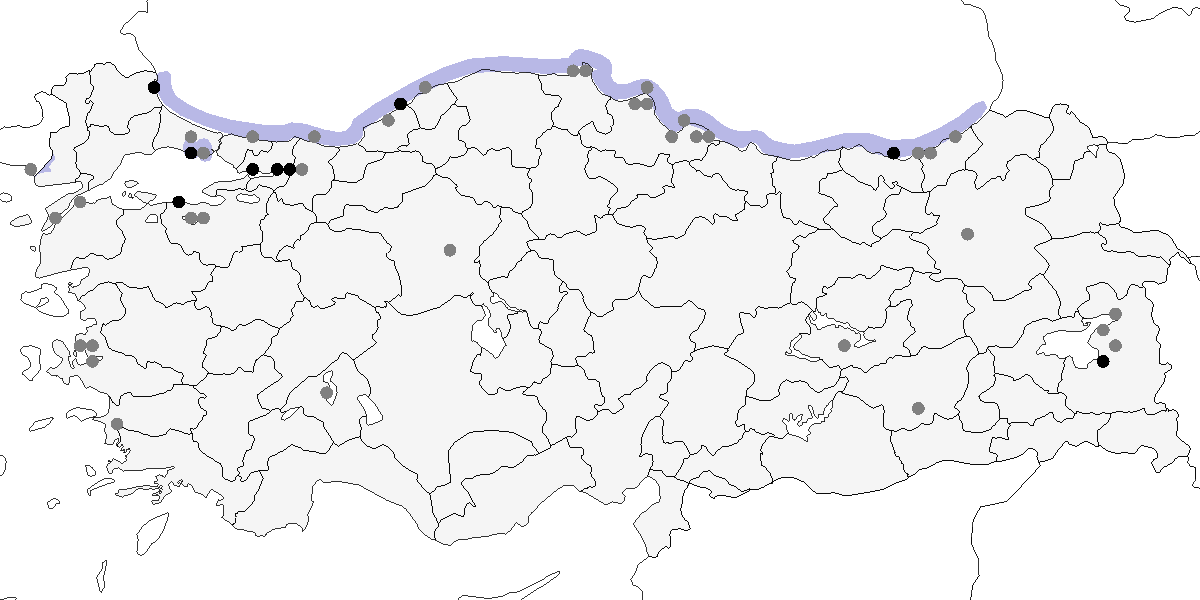
\includegraphics[keepaspectratio]{images/harita_Aythya marila.png}}

\textbf{Üreme}

Türkiye'de yuvalamaz. Avrasya ve Kuzey Amerika'nın kuzeyinde yuvalar.

\textbf{Alttürler ve Sınıflandırma}

Türkiye'de nominat alttürü bulunur.

\section{Pufla}\label{pufla}

\emph{Somateria mollissima}, Common Eider

\textbf{\emph{Karadeniz kıyılarında nadiren az sayıda görülür.}}

İlk üç kayıt şu şekildedir: 20 Eylül 1983'te Çernek Gölü'nde (Kızılırmak
Deltası) bir erkek (Dijksen \& Kasparek, 1985), 3 Ocak 1984'te Göksu
Deltası'nda ölü bir dişi (Kasparek, 1990a), 1 Şubat 1997'de Sakarya
Nehri deltasının batısında, Kefken açıklarında iyi tanımlanmış ilk
kışında bir erkek ve iki dişi (Welch \& Welch, 1998a) bulunmuştur.
Bundan sonra Riva, Terkos Gölü kıyıları, İğneada, Kızılırmak Deltası,
İzmit Körfezi ve Sakarya Karasu'da 20'den fazla kayıtta 1-3 birey tespit
edilmiştir.

Türkiye'de üremez, en yakın üreme kolonisi Ukrayna kıyılarındadır.
Güvenilir kayıtların tümü, 1975 yılında Ukrayna'nın Karadeniz kıyısında
bir üreme alanının keşfedilmesinden sonra olmuştur. Bu popülasyon
1990'ların ortasına kadar 1000 çifte ulaşmış ve günümüze kadar artmaya
devam etmektedir.

Şubat 1929'un ilk yarısında Tarabya ile Beykoz arasında (İstanbul
Boğazı) gözlenen bir erişkin erkek (Kumerloeve, 1970a), tanım olmadığı
için burada kabul edilmemiştir.

\pandocbounded{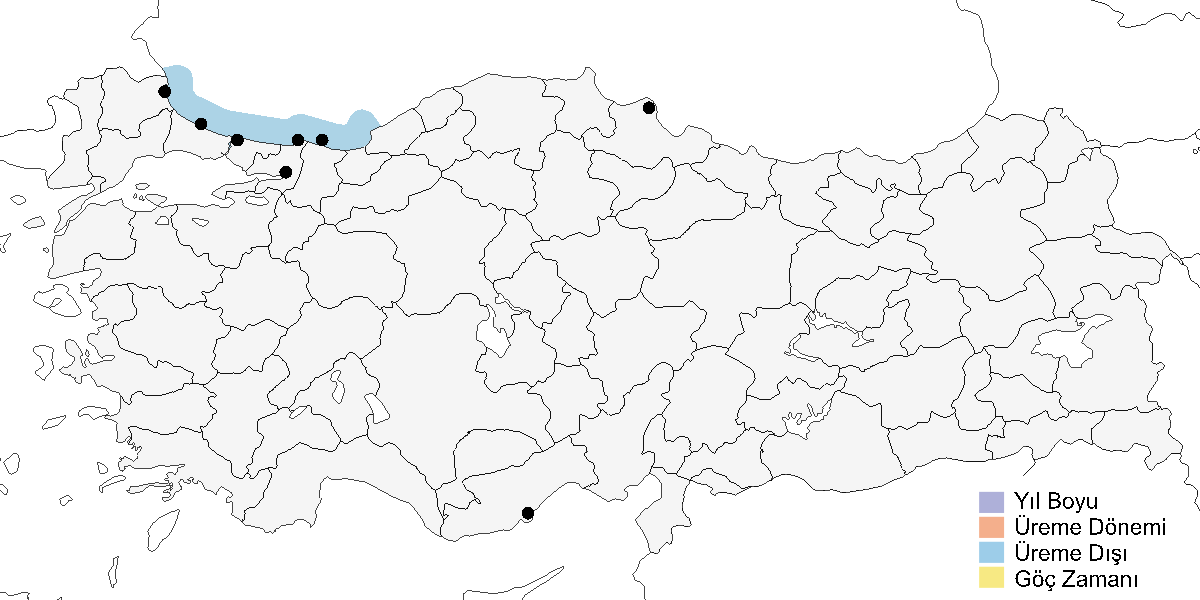
\includegraphics[keepaspectratio]{images/harita_Somateria mollissima.png}}

\textbf{Üreme}

Türkiye'de yuvalamaz. Ukrayna'daki koloni insan eliyle oluşturulmuş,
kolonideki kuşlar zamanlar doğallaşmıştır. Doğal yuvalama alanı Kuzey
Atlantik, Kuzey Buz Denizi ve Bering Boğazı'dır.

\textbf{Alttürler ve Sınıflandırma}

Ülkede gözlenen alttür nominat \emph{mollissima} (Kuzeybatı Avrupa)
alttürüdür.

\section{Kadife Ördek}\label{kadife-uxf6rdek}

\emph{Melanitta fusca}, Velvet Scoter

\textbf{\emph{Türkiye'de üreyen nüfus yok olmuştur. Karadeniz kıyılarına
az sayıda kışlar.}}

Doğu Anadolu'da az sayılarda kaydedilen çok lokal bir yaz konuğu idi. Az
sayıda yüksek irtifa göllerinde 3000 m'nin üstünde üremiş olduğu
düşünülür. Aktaş Gölü (Ardahan) kesin olarak ürediği tek alandır. 3 Ekim
1980'de 100 birey (Ven, 1980) ve 14-15 Temmuz 1994'te aralarında
gençlerin de bulunduğu 725 birey (Yarar, 1995) kaydedilmiştir.

Geçmişte Nemrut Dağı'ndaki (Tatvan) krater gölünde 20 çifte ürediği
düşünülmüştür. Ağrı Balık Gölü'nde geçmişte ürediği sanılmış, ancak
görünüşe göre Haziran 2001'de artık üremediğine karar kılınmıştır.
Çıldır Gölü'nde ürediği güçlü şekilde şüphelenilmiş, ancak teyit
edilmemiştir. Kars Aygır Gölü ve Muş Nazik Gölü'nde azami 32 birey yazı
geçirmiştir. Doğu Karadeniz kıyılarında kışlayan bireylerin yaz
aylarında da kaldığı gözlenmiştir.

Gürcistan'da yuvalamaya devam eden bireyler Karadeniz kıyılarına az
sayıda kışlar. Orta ve Doğu Karadeniz boyunca az sayıda kışlar. 1995
Aralık sonunda Yeşilırmak Deltası'nda 870 birey en yüksek kayıttır.
Nadir olarak Batı Karadeniz, Marmara'da ve güneyde Akdeniz kıyısında
kışlamıştır. Ocak 1970'te Burdur Gölü'nde 27 birey, Şubat 1966'da Mogan
Gölü'nde ve Ocak 2005'te Hazar Gölü'nde kaydedilmiştir. Son yıllarda
kaydedilen 50 birey.

4 Şubat 1917'de İstanbul Zeytinburnu açıklarında gözlenen iki birey ülke
için ilk kayıttır.

\pandocbounded{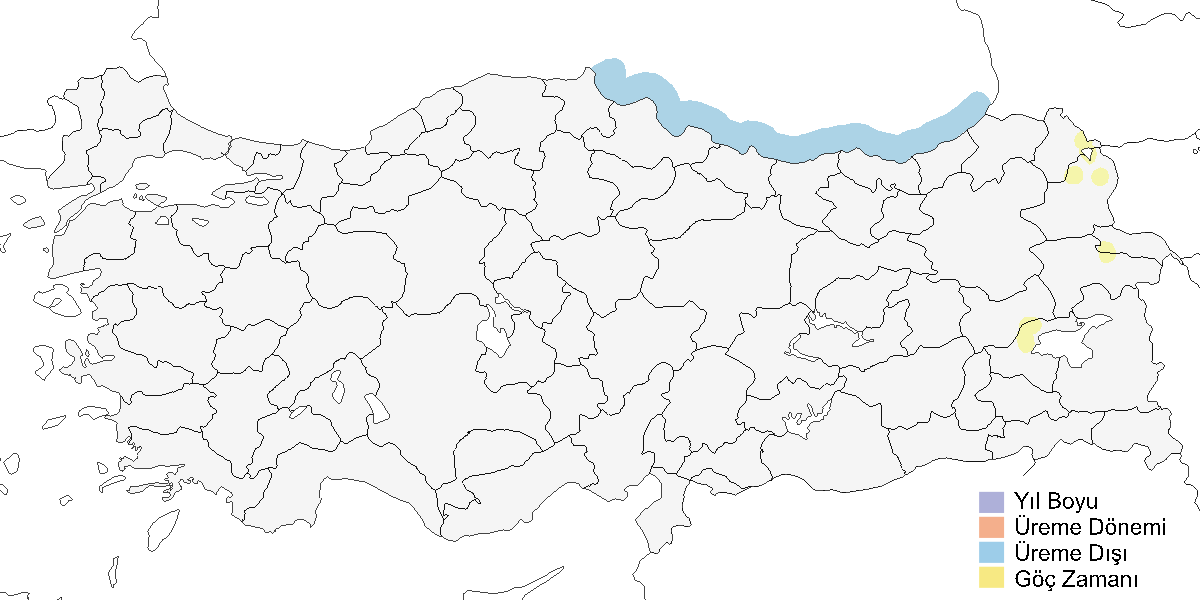
\includegraphics[keepaspectratio]{images/harita_Melanitta fusca.png}}

\textbf{Üreme}

\textbf{Yuvalama Alanı:} Doğu Anadolu'daki iki ya da üç yüksek irtifa
gölünde üremiştir. Tüm çabalara rağmen Türkiye'de yuvası bulunamamıştır.
Şu anda Kafkasya popülasyonu sadece Gürcistan'da bir gölde
yuvalamaktadır.\\
\textbf{Yuvası:} Türkiye'de yuva bulunmamıştır ancak diğer yerlerde
yoğun bitki örtüsünün içine gizlenmiş şekilde yerde ve genellikle
göllerdeki adalarda yuva yapar.\\
\textbf{Yumurta sayısı:} Olağan yumurta sayısı 7-10'dur.\\
\textbf{Üreme dönemi:} Eski gözlemlere göre temmuz ve ağustos ayında
yuvalamıştır. \textbf{DOA}. 10 Temmuz 1967'de Nemrut Dağı'ndaki krater
gölünde iki, yedi ve dokuz hav tüylü küçük yavru ile birlikte üç dişi ve
20 Ağustos 1967'de Balık Gölü'nde dört, beş ve altı yavrulu üç dişi
kaydedilmiştir (Vielliard, 1968). Küçük ördeklerin sadece yaklaşık bir
haftalık olduğu varsayılırsa yumurtlamanın haziranın ilk günlerinde
olduğu anlaşılmaktadır. 23 Ağustos 1972'de Nemrut Dağı'nda gözlenen
hemen hemen yarı gelişmiş yedi yavrulu bir dişi, yumurtlamanın haziranın
son haftasında olduğunu göstermektedir. 9 Temmuz 1985'te Nemrut Dağı'nda
beş çift ve iki genç birey gözlenmiştir. Son zamanlara ait bir üreme
kaydı yoktur ve 9 Haziran 2001'de Balık Gölü'ndeki adada yapılan
kapsamlı araştırmada ne yuva bulunmuş ne de erişkin görülmüştür.

\textbf{Alttürler ve Sınıflandırma}

Monotipik bir türdür. Eskiden Amerika ve Doğu Sibirya'da yaşayan Ak
Kanatlı Kadife Ördek \emph{Melanitta deglandi} ile aynı tür olarak kabul
ediliyordu.

\section{Kara Ördek}\label{kara-uxf6rdek}

\emph{Melanitta nigra,} Common Scoter

\textbf{\emph{Nadir kış konuğudur.}}

Karadeniz'de çoğunlukla eylül ve mart arasında çok az sayıda kaydedilen
kış göçmenidir. Düzenli olarak sadece Kızılırmak ve Yeşilırmak
deltalarının açıklarında 20 birey kışlamaktadır. Karadeniz kıyısında
toplam 20'den fazla kaydı vardır. Marmara ve Ege'de çok nadirdir,
Akdeniz'de sadece bir kere kaydedilmiştir.

9 Nisan 1967'de Kocaçay Deltası'nda kaydedilen bir birey ülke için kabul
edilebilir ilk kayıttır (OST, 1969). Öncesinde Ege'de nadir bir kış
göçmeni olduğundan (Krüper, 1875) ve İstanbul Boğazı ile Ceyhan
Deltası'ndaki şüpheli kayıtlardan (Kumerloeve, 1961) bahsedilmiştir.

\pandocbounded{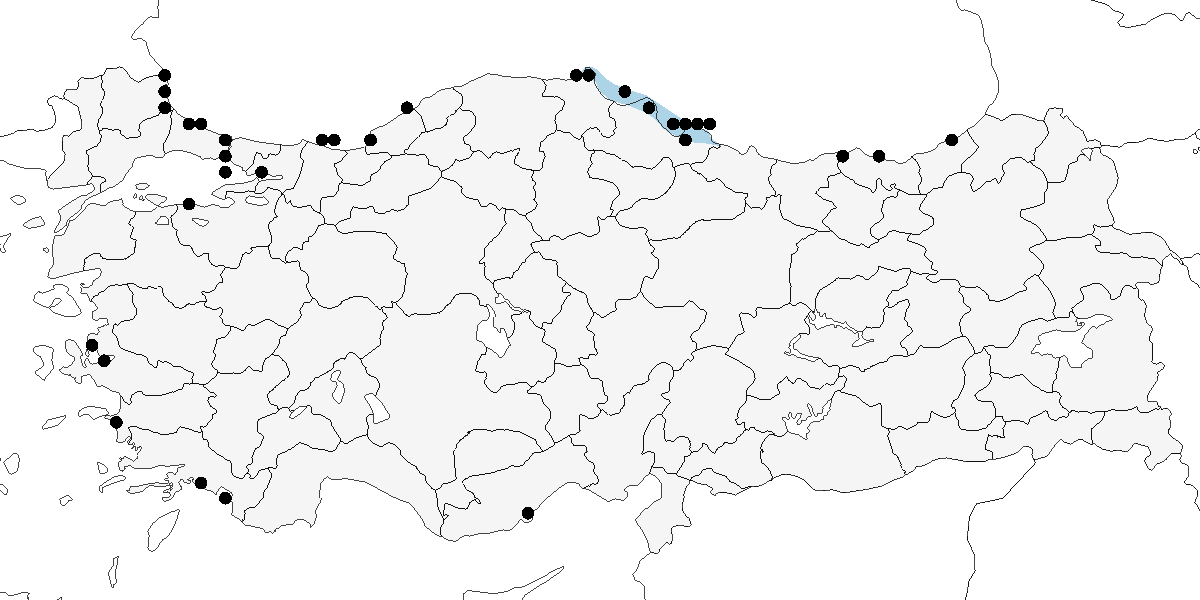
\includegraphics[keepaspectratio]{images/harita_Melanitta nigra.png}}

\textbf{Üreme}

Türkiye'de yuvalamaz. Avrasya'nın kuzeyinde yuvalar.

\textbf{Alttürler ve Sınıflandırma}

Monotipik bir türdür.

\section{Telkuyruk}\label{telkuyruk}

\emph{Clangula hyemalis}, Long-tailed Duck

\textbf{\emph{Nadir kış konuğudur.}}

Şubat 1893'te İstanbul (Büyük?) Çekmece'de, Alléon tarafından toplanan
genç bir dişi ülke için ilk kayıttır ve bu örnek Sofya Doğa Tarihi
Müzesi'nde görülebilir. Ardından, 13 Kasım 1968'de İzmit'te genç bir
birey kaydedilmiştir (OST, 1975). Göksu Deltası Paradeniz Gölü'nde 1-2
Ocak 1986'da bir birey ve 5 Ocak 1989'da bir dişi (Kasparek, 1990a)
görülmüştür. Sakarya Nehri ağzında 18 Şubat 2004'te (Balmer \& Betton,
2004b); 26 Şubat 2006'da Fırtına Nehri'nin ağzında birer birey
fotoğraflanmıştır. En güncel kayıtlara göre; 7-19 Ocak 2008'de
İğneada'da erişkin bir dişi, 13 Şubat 2008'de Kıyıköy'de bir erkek, 10
Aralık 2008'de İğneada'da bir birey (on üçüncü kaydı) ve 28 Mart 2009'da
Enez'de bir birey (on dördüncü kaydı) görülmüştür (Kirwan \& Özen,
2014).

İstisnai olarak, Van Gölü'nden 1977 ile 1987 arasında mayıs ve haziran
aylarında yaz kayıtları mevcuttur. 10 Haziran 1977'de Gevaş'ın batısında
Horkum'da iki birey ve Tatvan ile Ahlat arasında üç birey (Beaman,
1986), 22 Mayıs 1985'te Van'ın güneybatısında bir erkek (Martins, 1989),
9 Haziran 1987'de Van Sazlığı'nda bir erkek ve 22 Haziran 1987'de Van'ın
10 km güneyinde bir birey (Kirwan \& Martins, 1994) kaydedilmiştir.

\pandocbounded{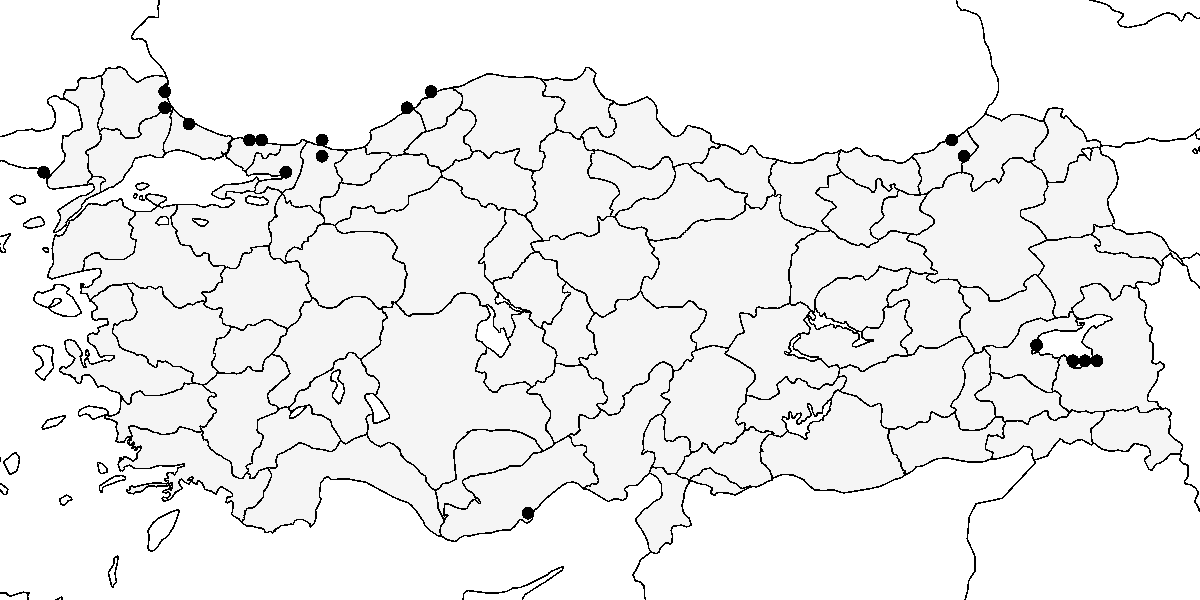
\includegraphics[keepaspectratio]{images/harita_Clangula hyemalis.png}}

\textbf{Üreme}

Türkiye'de yuvalamaz. Kuzey İskandinavya dağlarında ve Rusya ve Kuzey
Amerika'nın tundra kuşağında yuvalar.

\textbf{Alttürler ve Sınıflandırma}

Monotipik bir türdür.

\section{Altıngöz}\label{altux131nguxf6z}

\emph{Bucephala clangula,} Common Goldeneye

\textbf{\emph{Nispeten yaygın ve az sayıda kış konuğudur.}}

Karadeniz, Marmara ve Ege'nin kıyı bölgelerinde ve daha nadir olarak iç
bölgelerdeki sulakalanlarda ekim sonu ve nisan sonu arasında nadir bir
kış konuğudur. En düzenli olarak Marmara ve Karadeniz bölgelerinde
görülür. Kışın ülke çapında görülen kuş sayısı nadiren 100 bireyi geçer.
3 Şubat 1992'de Kızılırmak Deltası'nın açıklarında gözlenen 200 birey,
kaydedilen en yüksek sayıdır. 2005-06 kışında Gediz Deltası'nda 72
birey, 3 Şubat 2002'de Gala Gölü'nde 60 birey sayılmıştır (Demirci,
2002). Son yıllarda ilkbahar sonunda Doğu Karadeniz'de kaydedilmiştir.

1977 ile 1993 yılları arasında Doğu Anadolu'da, çoğunluğu Van Gölü'nde
olmak üzere, bir dizi yaz kaydı vardır ve bu kayıtlarda bazen birden
fazla birey gözlenmiştir. Bu kayıtlar, yakınlarda üreyen bir
popülasyonun ihtimalini düşündürmüştür (Kasparek, 1992a).

\pandocbounded{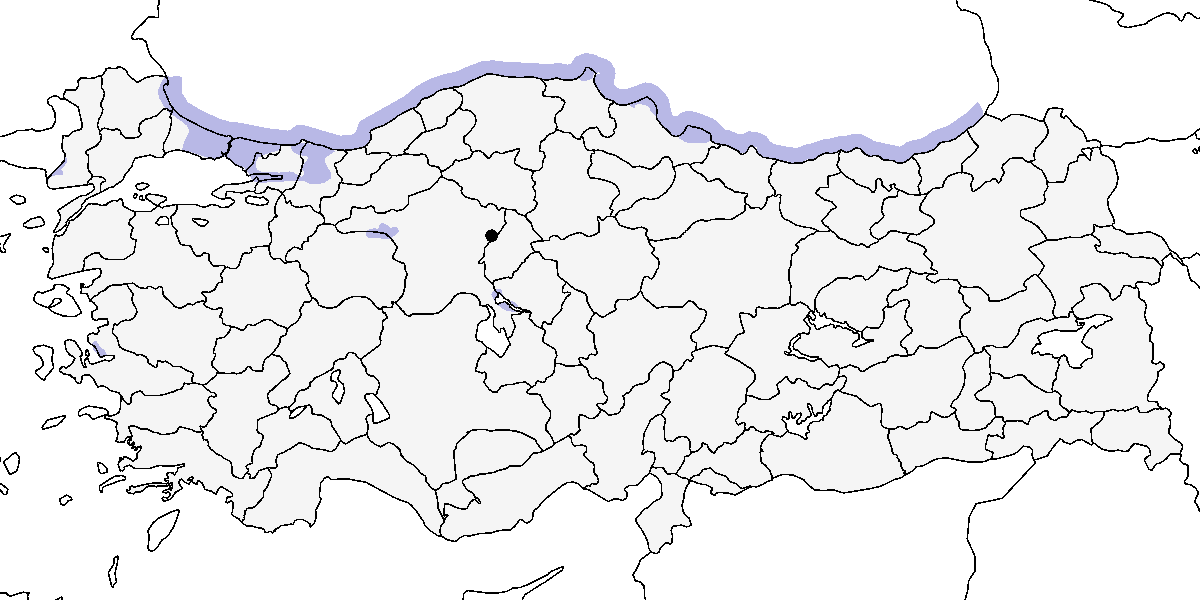
\includegraphics[keepaspectratio]{images/harita_Bucephala clangula.png}}

\textbf{Üreme}

Türkiye'de yuvalamaz. Avrasya ve Kuzey Amerika'nın kuzeyinde yuvalar.

\textbf{Alttürler ve Sınıflandırma}

Türkiye'de nominat alttürü bulunur.

\section{Sütlabi}\label{suxfctlabi}

\emph{Mergellus albellus,} Smew

\textbf{\emph{Kuzey bölgelerine az sayıda gelen bir kış konuğudur.}}

Kasımdan nisan ortasına kadar ülkenin batı ve orta bölgelerindeki
sulakalanlarda ve kıyılarda tipik olarak nadir ve muhtemelen düzensiz
bir kış konuğudur. En çok Marmara, Karadeniz ve İç Anadolu'da
kaydedilir. Her kış genellikle 100 bireyden daha azdır. Uluabat Gölü'nde
1967'de 300, 1969-70'te 1300, 1973'te 555, 1989'da 111 ve 1995'te 248
birey kaydedilmiştir. 1992'de Manyas Gölü'nde 102 ve 1993'te
Büyükçekmece'de 79 birey kışlamıştır.

Nisan 1987 sonunda Diyarbakır'da kaydedilmiştir. Doğu ve Güneydoğu
Anadolu'da oluşturulan büyük baraj göllerinde gözlenmesi beklenebilir.
Ocak 1979'da Irak Razzaza Gölü'nde gözlenen 1000'den fazla birey (Scott
\& Carp, 1982), daha güneyde yüksek sayılarda kaydedilebileceğini
göstermektedir.

Ancak ne tuhaftır ki, türün ilk keşfi Strickland tarafından İzmir'den
alınan iki örnek ile yapılmıştır. Cambridge Üniversitesi Zooloji
Müzesi'ndeki koleksiyonda bulunan bu örnekler, 6 Ocak 1836'da alınan bir
erkek ve aynı yıl şubat ayında alınan bir dişiye aittir. 1946-48
yıllarında Çatalağzı açıklarında (Zonguldak) oldukça bol olduğu
gözlenmiştir (Ogilvie, 1954).

11 Haziran 1969'da Eymir Gölü'nde (Ankara) bir erkek (OST, 1972), 27
Haziran 1987'de Göründü'de (Van) bir dişi (Kirwan \& Martins, 1994) ve
27 Mayıs 1995'te Uluabat Gölü'nde bir erkek ve iki dişi (Kirwan \&
Martins, 2000) olmak üzere yazın üç defa kaydedilmiştir.

\pandocbounded{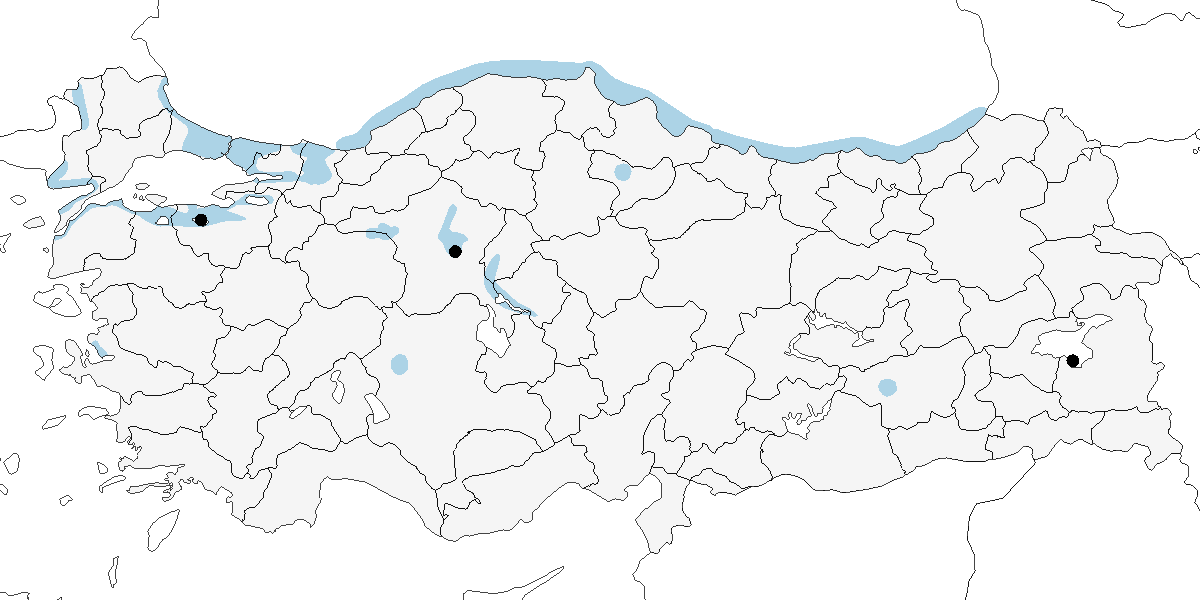
\includegraphics[keepaspectratio]{images/harita_Mergellus albellus.png}}

\textbf{Üreme}

Türkiye'de yuvalamaz. Avrasya'nın kuzeyinde yuvalar.

\textbf{Alttürler ve Sınıflandırma}

Monotipik bir türdür. Türkiye'de tanımlanmıştır.

\section{Büyük Tarakdiş}\label{buxfcyuxfck-tarakdiux15f}

\emph{Mergus merganser,} Common Merganser

\textbf{\emph{Nadir kış konuğudur.}}

Özellikle Marmara ve Karadeniz bölgelerinde az sayıda kaydedilen nadir
bir kış konuğudur. 1997-2007 arasında artan gözlemci aktivitesine karşın
sadece 10 kere kaydedilmiştir (Kirwan \emph{vd.}, 2003). Genellikle
kıyısal sulakalanlarda görülür ve en düzenli olarak Kızılırmak ve
Yeşilırmak deltalarında kaydedilir. Kızılırmak Deltası'nda görüldüğü en
geç tarih 20 Mayıs'tır.

Doğu Anadolu'da şubat ve martta iki defa, yazın ise üç kere
gözlenmiştir; 11 Haziran 1970'te Pasinler ile Horasan arasında Aras
Nehri üzerinde bir çift, 7 Haziran 1986'da Van Gölü'nde bir birey ve 29
Haziran 1988'de Bendimahi Deltası'nda bir dişi ya da genç birey
kaydedilmiştir. Kurutulmadan önce Sevan Gölü (Ermenistan) havzasında
üreyen bir tür olduğu düşünülmüş, ancak ürediğine dair bir kanıt elde
edilmemiştir (Adamian \& Klem, 1999).

\pandocbounded{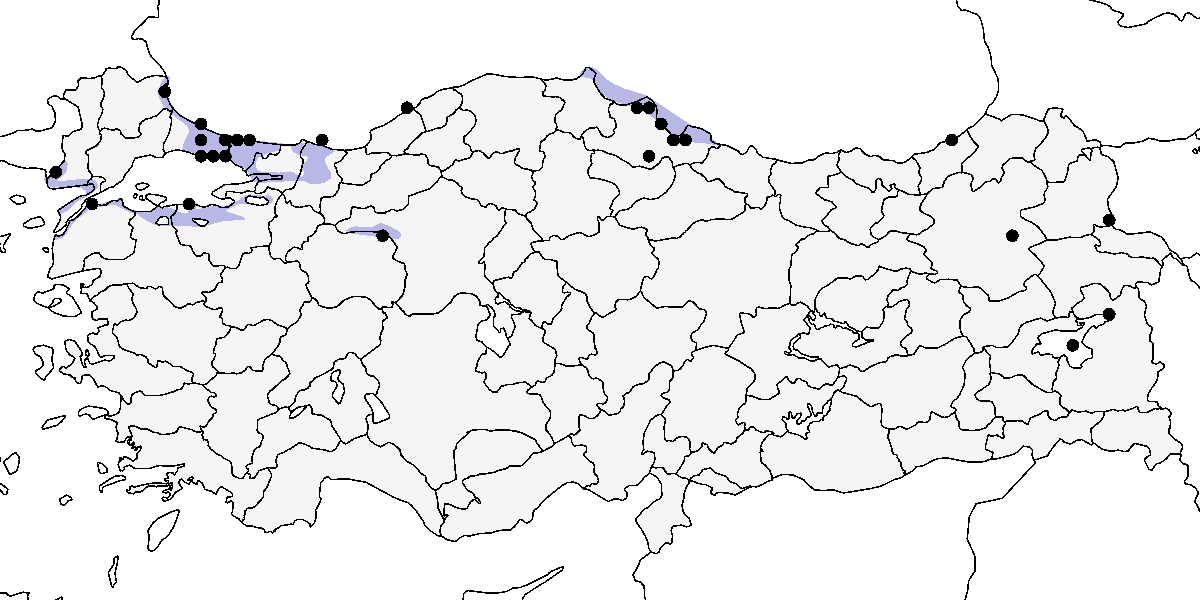
\includegraphics[keepaspectratio]{images/harita_Mergus merganser.png}}

\textbf{Üreme}

Türkiye'de yuvalamaz. Avrasya ve Kuzey Amerika'nın kuzeyinde yuvalar.

\textbf{Alttürler ve Sınıflandırma}

Türkiye'de nominat alttürü bulunur.

\section{Tarakdiş}\label{tarakdiux15f}

\emph{Mergus serrator}, Red-breasted Merganser

\textbf{\emph{Nispeten lokal olarak ve orta sayılarda görülen bir kış
konuğudur.}}

Kıyısal alanlarda ekim sonu ve nisan sonu arasında kaydedilen kış
göçmenidir. En çok sayıda Doğu Karadeniz, Marmara ve Ege'de kaydedilir.
Gediz Deltası'nda düzenli olarak yaklaşık 100 birey konaklar; Şubat
1996'da 397 birey sayılmıştır. Büyük Menderes Deltası'nda Şubat 1993'te
67 birey ve Yumurtalık'ta 44 birey kaydedilmiştir. Ege ve Doğu
Akdeniz'deki alanlarda düzenli olarak önemli sayılarda kışlar (Eken,
1997d). Akdeniz kıyılarında seyrek olsa da Kıbrıs'ta oldukça düzenli bir
türdür.

20-21 Mayıs 1994'te Göksu Deltası'nda geç kalmış bir birey
kaydedilmiştir (Birdquest Newsletter 23: 59). Tek yaz kaydı 11 Haziran
1964'te Amik Gölü'nde (Antakya) kaydedilen yedi veya sekiz bireydir
(Kumerloeve, 1966-67).

\pandocbounded{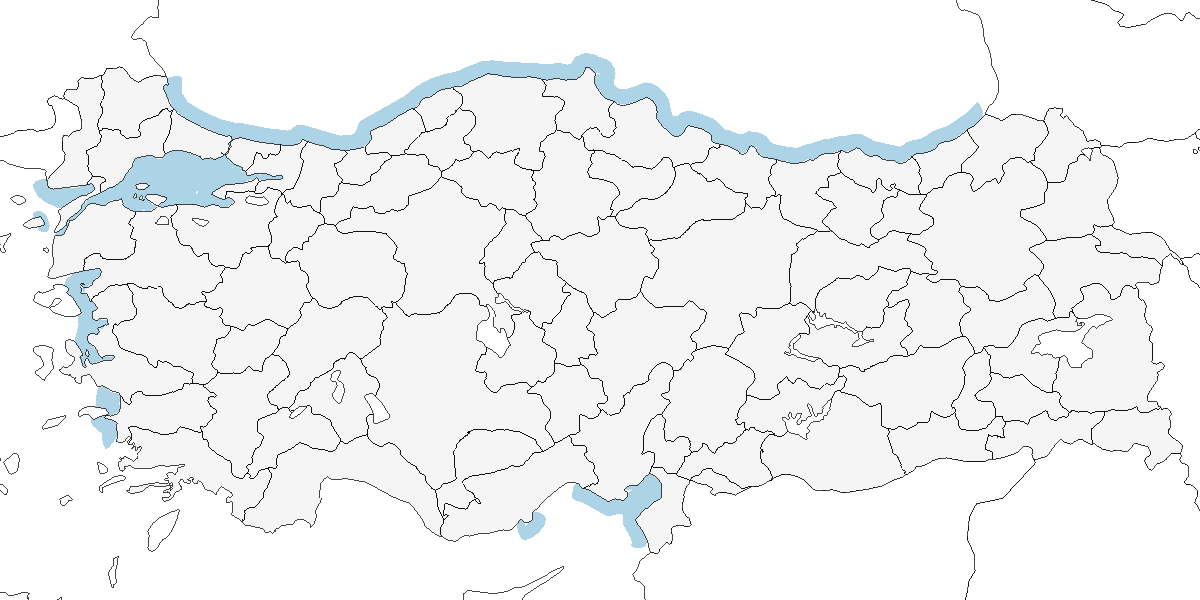
\includegraphics[keepaspectratio]{images/harita_Mergus serrator.png}}

\textbf{Üreme}

Türkiye'de yuvalamaz. Avrasya ve Kuzey Amerika'nın kuzeyinde yuvalar.

\textbf{Alttürler ve Sınıflandırma}

Monotipik bir türdür.

\section{Dikkuyruk}\label{dikkuyruk}

\emph{Oxyura leucocephala,} White-headed Duck

\textbf{\emph{Lokal olarak az sayıda üreyen yaz konuğu, nispeten yaygın
ve yüksek sayıda bulunabilen geçit türü ve kış konuğudur.}}

İç Anadolu ve Doğu Anadolu'da tatlı veya acı (sodalı), sığ ve ötrofik
göllerdeki yoğun sazlık sulakalanlarda az ila orta sayıda yuvalar. Van
Gölü çevresinde ve Kars'taki küçük sulakalanlarda ürediği teyit
edilmiştir. Doğu Anadolu'daki diğer alanlardaki üreme durumu
belirsizdir. Niğde Akkaya Barajı'nda üremiştir (Kirwan, 1994b). Üreme
döneminde kaydedildiği Karadeniz Bölgesi'ndeki bazı alanlarda
yuvalayabilir. Doğu Akdeniz sulakalanlarında yaz kayıtları, üremeyen
bireylere aittir.

1980'lerin sonu ve 1990'ların başı arasında dört kilit alanda (Ereğli
Sazlığı, Hotamış Gölü, Sultansazlığı ve Kulu Gölü) üreyen İç Anadolu
popülasyonu muhtemelen 150 çiftin üzerindeydi (Robinson \& Can, 1998).
Ancak 1990'ların ortasında Ereğli Sazlığı ve Hotamış Gölü'nün
kurumasıyla sayıları azalmış, Kulu Gölü'nde üremez olmuştur (Richardson,
2003). Kozanlı Gökgöl ve Uyuz Gölü'nde az sayıda üremeye devam
etmektedir.

Mart ile mayıs başı arasında birçok alanda geçiş sırasında gözlenir. 23
Mart 1992'de Kızılırmak Deltası'nda 1246 birey ve Mart 1990'da Ereğli
Sazlığı'nda 508 birey toplanmıştır. Mayıs ve haziran arasında toplanan
sürüler muhtemelen üreme alanlarına dağılacak kuşlardan oluşur. Temmuz
ve eylül arasında toplanan sürüler ise üreme sonrası dağılmaya ve göç
almaya işaret eder. Temmuzda Kulu Gölü'nde 500 birey ve ağustosta Sodalı
Gölü'nde 600-1000 birey kaydedilmiştir.

Kışın Akdeniz'deki birkaç sulak alanda yüksek sayıda, İç Anadolu'da
genellikle daha az sayıda kaydedilir. Batı ve orta bölgelerindeki diğer
yerlerde ise daha nadiren, özellikle sert hava koşullarında kaydedilir.
Karadeniz Bölgesi'nde düzensiz olarak yüksek sayılarda kışlar. Bir dönem
dünya popülasyonunun \%50'sinden fazlasının Burdur Gölü'nde kışladığı
düşünülmüştür; buradaki sayımlarda 1987'de 6400, 1988'de 9230, 1989'da
6700 ve 1991'de 10.927 birey kaydedilmiştir (Green \& Anstey, 1992).
Ancak 1992 sonrasında sayılarda azalma görülmüş; 1992'de 3264, 1993'te
3010 ve 1994'te 3337 birey sayılmıştır. Bu sayımlar son derece hassas
olup, eş zamanlı üç ekip tarafından ideal hava koşullarında
gerçekleştirilmiştir. Burdur Gölü'nde 1993'te 1991'e göre daha az genç
bireyin sayılması, daha düşük üreme başarısını gösterebilir. Bir
ihtimal, Kazakistan ve çevre ülkelerdeki üreyen nüfustaki azalış,
Türkiye'deki kışlama nüfusunun azalmasını açıklayabilir. Bu azalmada
şüphesiz kaçak avcılığın da payı vardır; 1992-93 kışında Burdur Gölü'nde
1000'den fazlasının vurulduğu tahmin edilmiştir. Ayrıca son yıllarda
Burdur Gölü'nün kuruma sürecinin başlaması ve tuzluluğun artması da bir
etken olabilir.

\pandocbounded{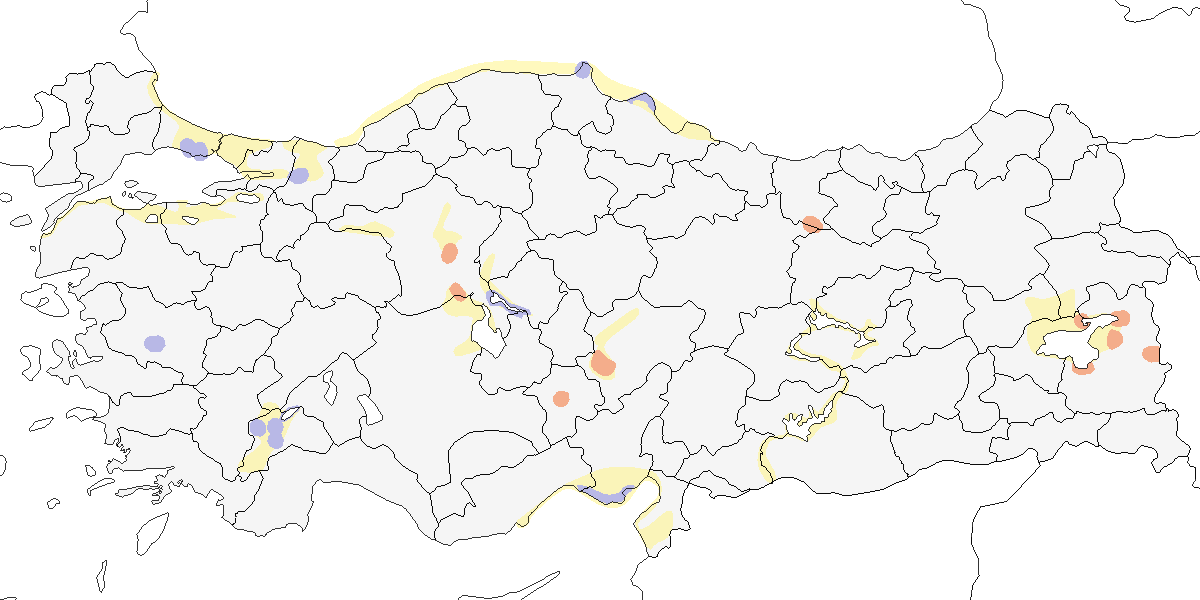
\includegraphics[keepaspectratio]{images/harita_Oxyura leucocephala.png}}

\textbf{Üreme}

\textbf{Yuvalama Alanı:} Çoğunlukla büyük sulak alanların yakınlarında
genellikle 10 hektardan küçük ve 2 metreden sığ, sualtı vejetasyonu bol
ve su aynalarının bulunduğu geniş sazlıklara sahip tatlı su göllerinde
ya da sodalı göllerde ürer (Anstey, 1989). Aynı alanda birkaç çift
üreyebilir.\\
\textbf{Yuvası:} Yuva, ölü saz gövdeleri ile diğer sucul bitkilerin
düzgün bir kâse oluşturacak şekilde örülmesi ile oluşturulmuş, birkaç
tutam açık gri tüy ile astarlanmış dayanıklı bir yapıdır.\\
\textbf{Yumurta sayısı:} Bir yuvada en fazla 10 yumurta kaydedilmiştir.
19 Haziran 2004'te aynı gölde diz boyu derinliğindeki suda yoğun bir
sazlığın içinde iyice gizlenmiş bir şekilde suyun üzerinde dikey
sazların dibine tutturularak yapılmış bir yuvada on yumurtalı
tamamlanmış bir kuluçka bulunmuştur. Diğer yerlerde olağan yumurta
sayısı 5-12'dir. Dikkuyruk, vücut ölçülerine göre son derece büyük ve
ağır yumurtalar koyar; yuva bu ağırlık nedeniyle suya batabilir.\\
\textbf{Üreme dönemi:} Mayıs başı ve temmuz başı arasında yumurta koyar.
Eylül sonuna kadar yavrular görülebilir. \textbf{İÇA:} 13 Temmuz 1987'de
Kulu Gölü'ndeki sazlıkların içindeki yuvada yedi yumurta gözlenmiştir;
muhtemelen dişinin kuluçkaya ara vermesi nedeniyle yuva ve yumurtalar
kısmen su altında kalmıştır (Anstey, 1989). Üreme kayıtlarının çoğu 3-10
yavrudan oluşan gruplardır: İç Anadolu'daki en erken kayıt, 5 Haziran
1975'te Kulu Gölü'nde gözlenen üç büyük ve üç hav tüylü yavrudur; bu
durum yumurtlamanın mayıs başında olduğunu gösterir. 6 Ağustos 1972'de
(kurutulmuş) Gönenç Gölü'nde 20 günlük beşer yavrularıyla iki dişi ve
dört günlük altı yavrulu bir dişi gözlenmiştir; bu kayıtlar
yumurtlamanın haziran ortası ile temmuz başında olduğunu göstermektedir.
İç Anadolu'da, temmuz ve ağustosta birçok yavrulu aile kaydedilmiştir.
\textbf{DOA:} Haziran-eylül ayları arasında Van Gölü'nde 9 Haziran 1987
ve 14 Haziran 1990'da gözlenen genç bireyler, yumurtlamanın mayıs
ortasında olduğunu göstermektedir. Temmuz-ağustos arasındaki diğer
kayıtlar, yumurtlamanın haziran ortasında başladığını düşündürmektedir.
Erçek Gölü yakınlarındaki küçük bir gölün ortasında dikey sazlardan
oluşan bir adada bir yuva bulunmuştur; sucul bitkiler kullanılarak
sazların dibine yapılmış olan yuvada 11 Haziran 2001'de iki yumurta
olduğu, kuluçkanın henüz tamamlanmadığı gözlenmiştir; alanda sekiz erkek
ve yedi dişi birey kaydedilmiştir. Ancak oldukça kapsamlı bir araştırma
yapılmasına rağmen başka bir yuva bulunmaması, üremenin henüz tam
anlamıyla başlamadığını göstermektedir.

\textbf{Alttürler ve Sınıflandırma}

Monotipik bir türdür.

\chapter{Tavukgiller, Kara
Kuşları}\label{tavukgiller-kara-kuux15flarux131}

\section{Orman Horozu}\label{orman-horozu}

\emph{Lyrurus tetrix}, Black Grouse

\textbf{\emph{Türkiye'de soyu tükenmiştir. Eskiden lokal olarak az
sayıda bulunan yerli türdü.}}

Relikt bir popülasyon, 19. yüzyılın sonuna kadar İstanbul çevresinde
devam etmiştir (Kasparek, 1990a), ancak anlaşıldığı kadarıyla avlanma
sonucunda soyu tükenmiştir. Türkiye'de yaşadığı ilk iki bilim insanı
tarafından tespit edilmiştir (Rigler, 1852; Tchihatchef, 1864). Son
olarak İstanbul Alemdağ çevresinde bulunduğu düşünülmüş (Reiser, 1904)
ve şehirde satılan, nereden geldiği bilinmeyen ölü erkek bireyler tespit
edilmiştir (Mathey-Dupraz, 1920--24). Aynı dönemde Bulgaristan
popülasyonunun da ciddi oranda azaldığı kaydedilmiştir (Elwes \&
Buckley, 1870); bu durum muhtemelen avcılığa bağlanmaktadır. Tür burada
da uzun süreden beri tükenmiş durumdadır. Genel olarak türün küresel
yayılış alanı kuzey ve batıya doğru daralmıştır (Hagemeijer \& Blair,
1997; Handrinos \& Akriotis, 1997; Madge \& McGowan, 2002).
Yunanistan'da 1935 yılından bu yana Selanik ve Rodop Dağları çevresinden
dört kayıt bulunmaktadır.

\pandocbounded{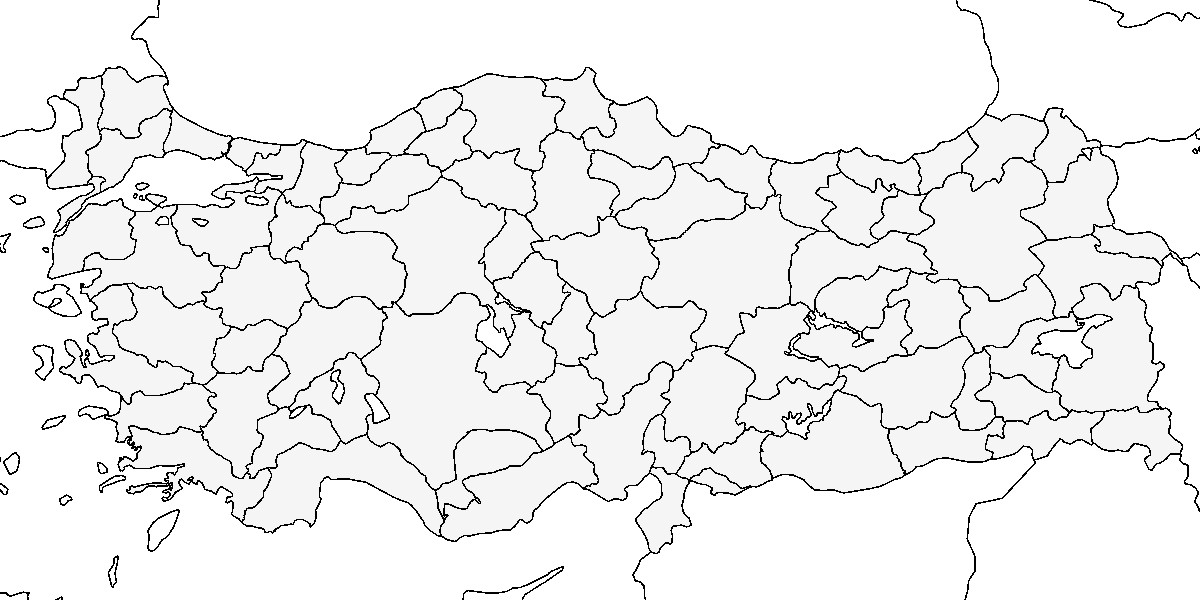
\includegraphics[keepaspectratio]{images/harita_Lyrurus tetrix.png}}

\textbf{Üreme}

Türkiye'de yuvalamaz. Kuzey Avrasya'daki orman kuşağında yuvalayan yerli
bir türdür.

\textbf{Alttürler ve Sınıflandırma}

Türkiye'de yaşamış popülasyon muhtemelen nominat \emph{tetrix} alttürüne
aittir. Literatürde \emph{Tetrao} cinsi altında da sınıflandırılmıştır.

\section{Dağ Horozu}\label{daux11f-horozu}

\emph{Lyrurus mlokosiewiczi}, Caucasian Grouse

\textbf{\emph{Lokal olarak az sayıda bulunan yerli bir türdür.}}

Doğu Karadeniz Dağları'nın kuzey yamaçlarında bulunur. Ağaç sınırının
üstündeki 1800-3000 metre arasındaki ormangülü (\emph{Rhododendron})
örtüsünde yaşar. 3000 metre üzerinden gelen üreme kayıtları (Başkaya,
2003) doğrulama gerektirir; ancak, neredeyse yerleşim yerlerine yakın
(muhtemelen 15 kilometreye kadar) ve sonbahar ile kış mevsimlerinde
düşük yüksekliklerde, ağaç sınırının altında ve muhtemelen özellikle
şiddetli soğuklarda daha da düşük yüksekliklerde bulunurlar. Yayılış,
bodur ormangülü \emph{Rhododendron} ile alpin çayır kuşağının altındaki
huş (\emph{Betula}) içeren yamaçlar üzerine yoğunlaşmıştır (Atkinson
\emph{vd.}, 1995).

Artvin'in güneydoğusundan Gürcistan sınırı üzerinde Posof'a kadar
Yalnızçam Dağları'nda dar bir alanda bulunurlar. Yerel halktan alınan
bilgiler ışığında Gümüşhane'nin batısında, Giresun çevresinde ve
muhtemelen Bingöl'e kadar güneyde, Cilo Dağları'nda bulunması olasıdır.

Türün lokal olarak nadir ya da Doğu Karadeniz kıyı şeridi boyunca yaygın
yerli olduğu gösterilene kadar, geçtiğimiz yıllar içerisindeki
kayıtlarda görülen aşırı düzeydeki yetersizlik ile özellikle 1980 öncesi
kayıtlardaki eksiklik, türün Türkiye'de çok az bilinmesine neden
olmuştur. G. Neuhäuser, Eylül 1943 tarihinde yüksek olasılıkla Türkiye
için ilk kayıt olan bir çift huş tavuğunu Rize ve Erzurum arasındaki
dağlardan toplamıştır (Kumerloeve, 1961).

Türkiye popülasyonunun muhtemelen \%90'ının görüldüğü Kaçkar
Dağları'nda, özellikle Sivrikaya çevresinde, 1993 yılında
gerçekleştirilen gözlem çalışmalarında kur yapma amacıyla bir araya
toplanan (lek poligini) 134 erkek gözlenmiştir. O tarihlerde yapılan
tümevarımla toplam popülasyonun 2000 bireyden fazla olduğu tahmin
edilmiştir (Magnin \& Yarar, 1997). Türkiye popülasyon büyüklüğü, son
zamanlardaki çalışmalara göre 1508-2675 birey arasında ölçülmüş ve tür
45 coğrafi yerde kaydedilmiştir (Isfendiyaroğlu, Welch \& Atad, 2007).
Bu coğrafi yerlerin 29 tanesi yakın bir zaman dilimi içerisinde
keşfedilmiştir. Bunlardan 4 tanesi nispeten ayrık popülasyonlardır.
Türün yayılış sınırlarını ve popülasyon büyüklüğünü tam olarak
belirlemek için bilgisayar modellemesi kullanılmıştır (Gottschalk
\emph{vd.}, 2007). Ancak, modellemenin sonuçları bilinen ve yayılış
haritasında gösterilen alanı genişletilememiştir. Bununla birlikte 4900
bireylik popülasyon tahmini, önceki en iyimser tahminlerden bile çok
yüksek olmuştur.

Türkiye popülasyonu, yaylaların tatil konutlarına dönüşmesi sonucunda
artan yol inşaatları nedeniyle yaşam alanlarının terkedilmesinden
etkilenmekte ve nesli tehlike altına girmektedir. Daha az ölçüde avlanma
baskısından (özellikle sonbahar döneminde görülen bir problem) ve tür
için bir tehdit kaynağı olarak listelenen aşırı otlatma bugün kaydedilir
ölçekte değildir; ancak, bu durumun izlenmesi gereklidir. Türün
popülasyonlarının dengede ya da azalmakta olup olmadığını ortaya koymak
için türün popülasyonu ve yayılışı ile ilgili tarihsel bilgiler yetersiz
düzeydedir; ancak, popülasyonların azalmasından şüphelenilmektedir.

\pandocbounded{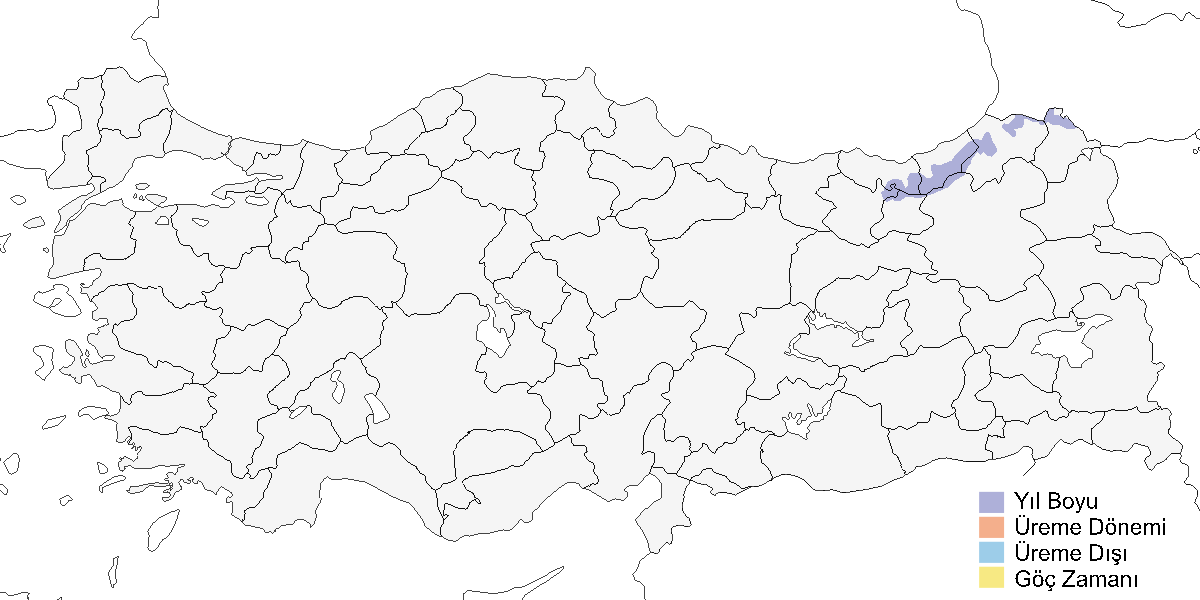
\includegraphics[keepaspectratio]{images/harita_Lyrurus mlokosiewiczi.png}}

\textbf{Üreme}

\textbf{Yuvalama Alanı:} Türkiye'de sadece iki yuvanın en iyi bilindiği
lokalite, Sivrikaya'da (Rize) bulunmuştur. İlk yuva 2800-3000 metrede,
bodur \emph{Rhododendron} çalılarının bulunduğu 3 hektarlık bir alanda
yer almıştır.\\
\textbf{Yuvası:} Yuva, yoğun, kısa (1 metre) ve çok dallı çallılarda
iyice gizlenmiş olup, kökten çıkan dalların arasında, zeminde sığ bir
çanak şeklinde yapılmış, kuru dallar ve birkaç kuru \emph{Rhododendron}
yaprağıyla astarlanmıştır.\\
\textbf{Yumurta sayısı:} Bu yuvada 6 Temmuz 1991 tarihinde 5 yumurta
kaydedilmiştir (Temple-Lang \& Cocker, 1991).\\
\textbf{Üreme dönemi:} Erkekler, özellikle şafak ve gün batımında,
eşeylerin çiftleşme amaçlı karşılaştığı alanlarda bir araya gelerek kur
gösterileri (nümayiş) yaparlar. Diğer kayıtlarda dişinin uçarak
uzaklaştığı bir yuvada 12 Temmuz 1993 tarihinde 4 yumurta görülmüş ve
bir yumurta kabuğu 11 Haziran 1997 tarihinde bulunmuştur. Bir erişkin
dişi ile tam gelişmemiş iki genç, 12 Haziran 2003 tarihinde Ardahan,
Posof'da gözlenmiş ve yumurtlama zamanının mayıs başında başladığını
göstermiştir. Başka yerlerde, yaygın kuluçka küme büyüklüğü 5-6 (2-10)
adettir. Ermenistan'da, 30 Mayıs 1984'te bulunan bir yuva 8 yumurta
içermiş ve bu yuvada ilk yumurtanın 21-23 Mayıs 1984 tarihinde
bırakıldığı belirlenmiştir. Bir diğer yuva 20 Mayıs 1985 tarihinde
yumurta içermekte olup, ilk yumurta 13-16 Mayıs 1985 tarihinde
bırakılmıştır. Bir dişi üç genç bireyle (ergin büyüklüğünün \%25'ine
ulaşmış) birlikte 5 Haziran 1980 tarihinde ve bir diğeri 26 Temmuz 1980
tarihinde tamamiyle büyümüş 5 genç içermektedir (Adamian ve Klem 1999).
Ermenistan'dan üreme döneminin daha erken gösteren kayıtlar, Türkiye
kayıtlarının normal üreme dönemini yansıtıp yansıtmadığı hakkında bazı
şüpheleri ortaya koymuştur.

\textbf{Alttürler ve Sınıflandırma}

Monotipik bir türdür. Rusca literatürde çoğunlukla \emph{Lyrurus} cinsi
altında, Batı Avrupa'da \emph{Tetrao} altında sınıflandırılmıştır.
Farklı uygulamaların özeti için bkz. (Gokhelashvili, Reese \&
Gavashelishvili, 2003).

\section{Çilkeklik}\label{uxe7ilkeklik}

\emph{Perdix perdix}, Grey Partridge

\textbf{\emph{Lokal olarak az sayıda bulunan bir yerli türdür.}}

Özellikle ovalardaki tarım alanlarında, uzun boylu ot topluluklarının
kenarlarında ve 2250 metreye kadar birincil yarı step alanlarda ürer.
Özellikle İç Anadolu ve Doğu Anadolu'nun kuzey kısımlarında ve Karadeniz
Bölgesi'nin iç kısımlarında yuvalar. Güney Anadolu'daki yayılış alanının
çoğunda ise çok nadir ve lokaldir.

Geçtiğimiz 20 yıl içerisinde tarımın yoğunlaşması, aşırı otlatma ve
avlanma nedeniyle popülasyonu önemli derecede azalmıştır. Trakya'da
yabani nesli tükenmiş olup, çeşitli kurum ve kuruluşlar tarafından
nüfusu takviye amaçlı genetik yapısı farklı olan yetiştirilmiş kuşlar
salınmış, ancak bu kuşlar yeni bir nüfus oluşturamamıştır. Belki de
Bulgaristan'daki yabani kuşların Türkiye'ye kendiliğinden gelmesi
beklenmelidir.

\pandocbounded{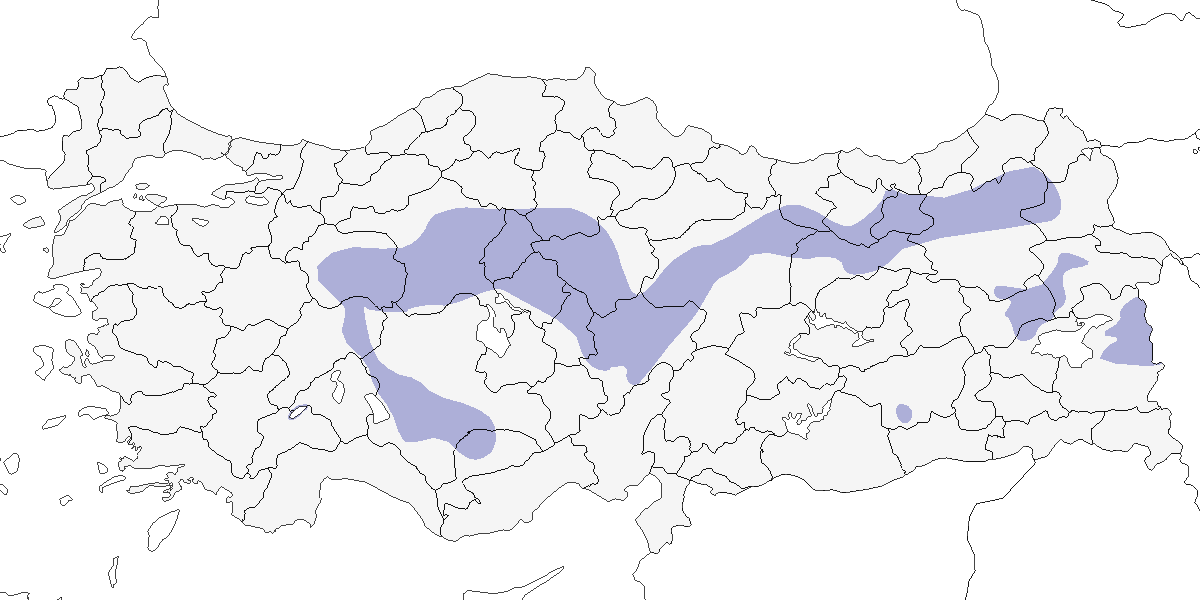
\includegraphics[keepaspectratio]{images/harita_Perdix perdix.png}}

\textbf{Üreme}

\textbf{Yuvalama Alanı:} Genellikle açık tarım alanlarında ürer.\\
\textbf{Yuvası:} Türkiye'deki bir yuvası betimlenmemiştir, ancak diğer
yerlerden gelen bilgilere göre yuva, ot ve ölü yapraklarla astarlanmış,
genellikle vejetasyon içerisine iyi bir şekilde gizlenmiş ve zeminde yer
alan sığ oyuklar şeklindedir.\\
\textbf{Yumurta sayısı:} 19 yumurta koyabilir. Diğer yerlerdeki yaygın
kuluçka küme büyüklüğü 9-20 (23) arasındadır. Bazen iki dişinin aynı
kuluçkayı paylaşması nedeniyle büyük kuluçkalar da kaydedilebilir.\\
\textbf{Üreme dönemi:} Mayıs ayında yumurtlamaya başlar. Yavrular:
\textbf{İÇA:} 11 Haziran 1977 tarihinde bir genç ile bir ergin Mogan
Gölü'nde, 16 Temmuz 1977 tarihinde 8 genç Emir Gölü'nde ve 28 Ağustos
1984 tarihinde 7 bireylik bir aile Çavuşcu Gölü'nde kaydedilmiştir.
\textbf{GDA:} Diyarbakır yakınlarında, 16 Mayıs 1999 tarihinde gevenle
(\emph{Astragalus sp.}) örtülü bir yamaçta on yumurta içeren bir yuva 27
Mayıs'ta 19 yumurta içermiştir (Karakaş \& Kılıç, 2002).

\textbf{Alttürler ve Sınıflandırma}

Trakya'da nominat \emph{perdix} alttürü, Anadolu'da ise \emph{canescens}
alttürü bulunmaktadır. Doğaya salınan farklı orijinden bireylerin yerel
kuşlarla karışması nedeniyle türün yayılış alanı içindeki coğrafi
varyasyonu oldukça karışıktır (Madge \& McGowan, 2002).

\section{Sülün}\label{suxfcluxfcn}

\emph{Phasianus colchicus}, Common Pheasant

\textbf{\emph{Lokal olarak az sayıda bulunan yerli türdür.}}

Türkiye'deki yerli popülasyonun yayılış alanı büyük ihtimalle Batı ve
Orta Karadeniz kıyısındaki kıyısal ormanlar, ``psödomaki'' olarak
bilinen Akdeniz bitki örtüsü ve fundalıklarla sınırlıydı. Tüm bilinen
tarihi ve güncel lokaliteler haritalanmıştır (Kasparek, 1988b), bu
yayılış noktalarının çoğu Güney Marmara ve Orta Karadeniz'de yoğunlaşmış
olup, en batıda Trabzon'a kadar doğuya ulaşır. Türkiye'deki yerli bir
popülasyonun varlığı bir dönem şüpheyle karşılanmışsa da (Madge \&
McGowan, 2002), İstanbul bölgesinden 1792'den sonra gelen kayıtlar yerli
popülasyonun varlığını desteklemiştir (Kasparek, 1988b).

Doğal nüfusu neredeyse tamamen kaybolmuştur; yabani kuşların çoğunun
soyu av için salınan kuşlara dayanır. Toplam stoktaki yerli kuşların
varlığı çok sınırlıdır ve saf yerli kan, devamlı olarak av için salınan
yabancı ve karışık kuşların içinde eriyip gitmiştir. Bugün doğal
popülasyondan geriye kalanların Sinop bölgesinde ve yakın zamana kadar
Kızılırmak Deltası ve çevresinde bulunması olasıdır. İç Anadolu, Ege ve
Akdeniz'de görülen sülünler, şüphesiz doğaya salınan kuşlardan
türemiştir.

\pandocbounded{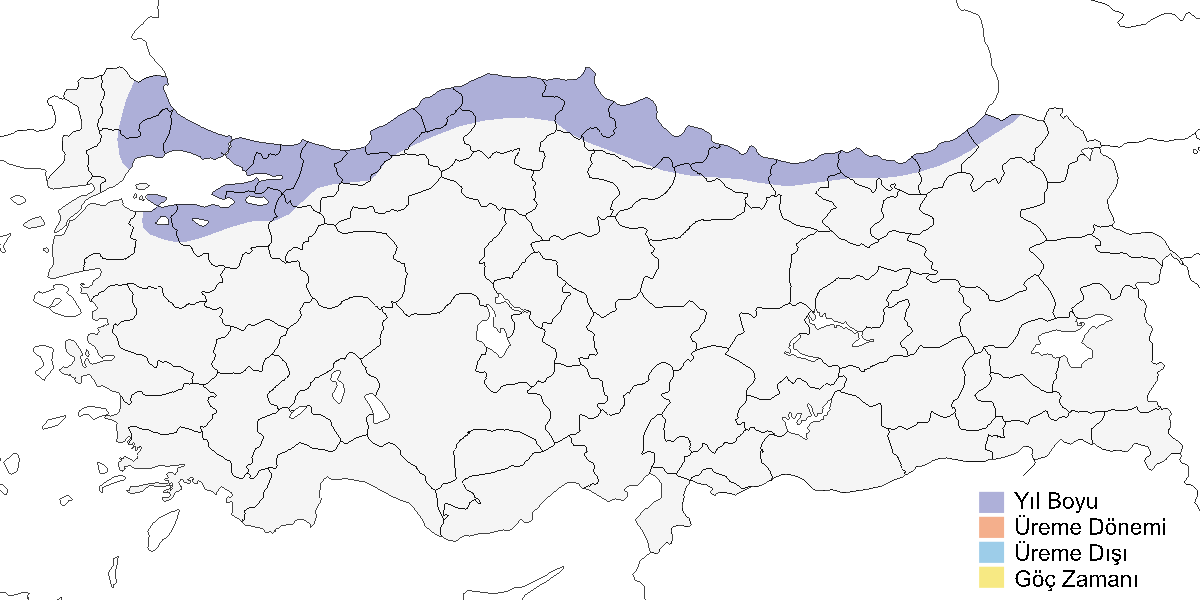
\includegraphics[keepaspectratio]{images/harita_Phasianus colchicus.png}}

\textbf{Üreme}

\textbf{Yuvalama Alanı:} Kıyısal ormanlar, ``psödomaki'' olarak bilinen
Karadeniz bitki örtüsü ve fundalıklar.\\
\textbf{Yuvası:} Bu konuda Türkiye'den bir bilgi yoktur. Zemine
yuvalar.\\
\textbf{Yumurta sayısı:} Diğer yerlerde 6-11 yumurta koyar.\\
\textbf{Üreme dönemi:} Diğer yerlerde mayıs ve haziran arasında yumurta
koyar.

\textbf{Alttürler ve Sınıflandırma}

Yerli popülasyon, nominat \emph{colchicus} alttürü altında
sınıflandırılmıştır (Dement'ev \& Gladkov, 1967; Roselaar, 1995). Hatalı
olarak Kuzey Kafkasya'da bulunan \emph{septentrionalis} alttürüne dahil
edilmiştir (Kumerloeve, 1961).

\section{Turaç}\label{turauxe7}

\emph{Francolinus francolinus}, Black Francolin

\textbf{\emph{Güneydoğu Anadolu ve Doğu Akdeniz'de yaygın olarak çok
sayıda bulunan yerli türdür.}}

Çukurova ve Göksu Deltaları çevresinde, ayrıca Suriye sınırında Fırat ve
Dicle nehirleri boyunca ürer. Doğu Akdeniz popülasyonu en iyi
izlenendir. Çukurova popülasyonunun 75 çiftinin Akyatan Gölü çevresinde
yoğunlaştığı, toplamda 85 çifte ulaştığı kaydedilmiştir (Magnin \&
Yarar, 1997). Göksu Deltası'nda, çoğu kumullarda olmak üzere 50 üreme
çifti kaydedilmiştir (Magnin \& Yarar, 1997). En yaygın bulunduğu bölge
olan Güneydoğu Anadolu'da yaklaşık 15 lokaliteden kaydı vardır (Welch,
2004).

Doğu Akdeniz'deki popülasyonu dikkate alınarak mevcut durumu ve
ekolojisi derlenmiştir (Berk, 1988). Doğu Akdeniz'deki bazı yerlerde tür
için koruma tedbirleri uygulanmıştır. Güneydoğu Anadolu'da ise tarımsal
faaliyetlerin artması sonucu hem sayılarının arttığı hem de yayılış
alanının genişlediği düşünülmektedir.

Eskiden Güneydoğu Marmara ile Ege Bölgesi'nin güney kıyılarının bazı
bölümlerinde yerli olarak kaydedilmiştir (Kumerloeve, 1963b). Ancak, her
iki bölgede 19. yüzyıl içinde ortadan kalkmıştır. İstanbul Boğazı
çevresinden 1850'li yıllardan gelen tek bir kayıt vardır. Göller Bölgesi
ile Anti-Toroslara kadar kuzeyde, 600 metreye kadar oldukça lokal olarak
kaydedilmiştir (Kumerloeve, 1961). Ekim 2003 tarihinde Tavas, Denizli
çevresinden muhtemelen tutsak bir bireyin kaçması sonucu güncel bir
kayıt gelmiştir. 1960'lı yıllarda Köyceğiz Gölü'ndeki kayıtlar, Batı
Akdeniz'deki son kayıtlardır. 1990'lı yıllara kadar Akdeniz bölgesindeki
yayılışı İçel, Adana, Osmaniye ile sınırlıydı. Sayıları artan kuşların
yavaş yavaş Batı Akdeniz'e doğru ilerlediği kaydedilmiştir. Örneğin
Antalya Havaalanı arazisinde 2010'dan beri kaydedilmektedir.

\pandocbounded{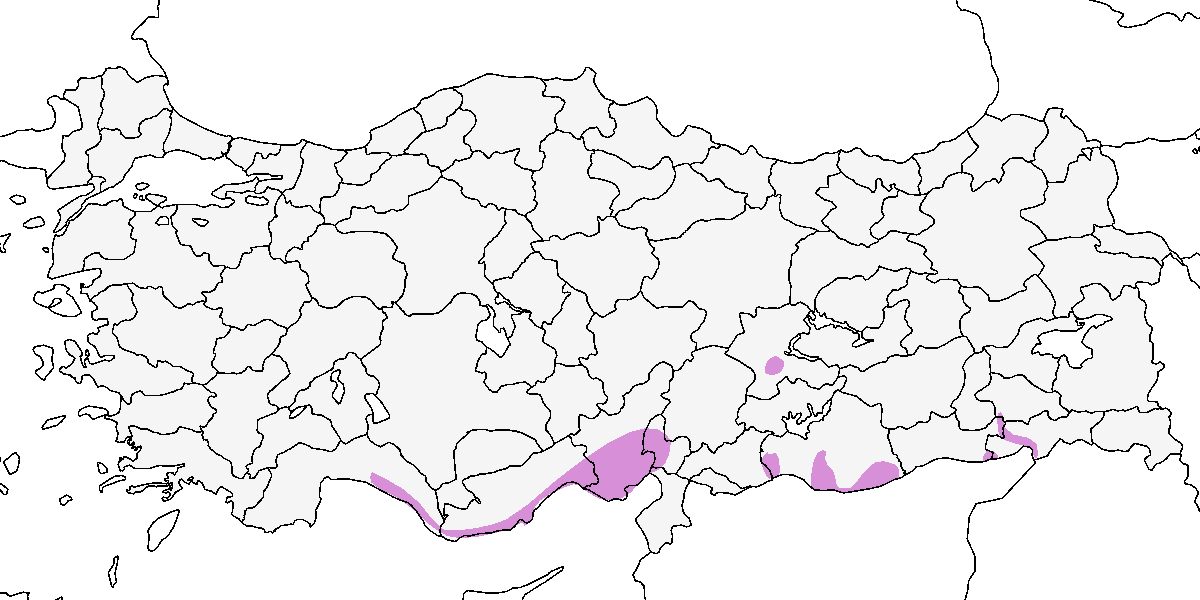
\includegraphics[keepaspectratio]{images/harita_Francolinus francolinus.png}}

\textbf{Üreme}

\textbf{Yuvalama Alanı:} Çalı ve çalı dışındaki bitki örtüsüne sahip
kumullar ile ot, çalı ve bodur bitkilerin arasındaki oyuklarda yaşarlar.
Ayrıca, olgunlaşmamış çalıların bulunduğu nemli (ıslak olmayan) alanlar,
nehir kıyıları ve sık ılgın (\emph{Tamarix}) çalılarından oluşmuş sık
topak şeklindeki çalılık alanlarda ve mısır tarlalarında ürerler. Kum
tepelerinde (her 2-5 hektarda bir erkek) ve tarım alanlarında (15-30
hektarda bir erkek) yüksek yoğunluktadırlar (Berk, 1988).\\
\textbf{Yuvası:} Göksu Deltası'ndaki kum tepelerinde 17 Haziran 1992
tarihinde bulunan eski yuva, astarlanmamış, kum içerisinde birkaç bitki
parçasıyla çevrelenmiş sığ bir oyuk şeklindedir ve zemininde bir tutam
ot içermektedir.\\
\textbf{Yumurta sayısı:} Türkiye dışında yumurta sayısının genellikle
8-12 arasında olduğu bilinir.\\
\textbf{Üreme dönemi:} Mart sonu ve nisan arasında yumurta bırakır.
Yavrular mayıs ortasında dolaşmaya başlar ve temmuz ortasına kadar
görülebilir. Manchester Müzesi'ndeki üç yumurta (tamamlanmamış bir
kuluçkadan) İzmir yakılarından 10 Mayıs 1899 tarihinde alınmıştır. Tring
Doğa Tarihi Müzesi'ndeki dört yumurtanın ikisi Mersin'den 7 Mayıs 1884
tarihinde ve diğer ikisi 15 Mayıs 1899 tarihinde Anadolu'da bilinmeyen
bir lokaliteden alınmıştır. \textbf{AKD:} Göksu Deltası'ndaki kum
tepelerinde, 17 Haziran 1992 tarihinde muhtemelen bir önceki yıldan
kalmış bir yuva kaydedilmiştir. Yuvada güneşten etkilenmiş ve solgun
renklere sahip yumurta kabukları bulunmuştur. Yuva, astarlanmamış, kum
içerisinde birkaç bitki parçasıyla çevrelenmiş sığ bir oyuk şeklindedir
ve zemininde bir tutam ot içermektedir. Göksu'da, en azından 1-2 günlük
7 genç ile bir dişi 5 Mayıs 2004 tarihinde kaydedilmiştir. Bu kayıt, ilk
yumurtanın 9 Nisan'da bırakıldığını göstermektedir. Bir ergin ile bir
genç kuş 20 Temmuz 1986 tarihinde gözlenmiştir. Çukurova'da, yerel halk
yavruları 10 Mayıs 1986 tarihinde yakalamıştır (yaygın oldukları
bildirilmiştir). Bu tarih, yumurta bırakma zamanının yaklaşık nisan
ortasında olduğunu göstermektedir. Ötüşteki artış ise nisan ayının
ikinci yarısı ile mayıs ayının ilk yarısında tepe yapmaktadır (Berk,
1988). Eski avcıların kayıtlarına göre ``dişi kuşlar mart sonu ile nisan
ayı içerisinde yuvaları ve yumurtaları ile meşguldürler'' (Banoğlu \&
Burr, 1953). Yumurtalar, keklik (kınalı keklik) yumurtaları büyüklüğünde
ve açık yeşil renktedir; Seyhan ve Ceyhan kıyılarındaki sık örtüşe sahip
bodur ağaçlıklar arasında zemine bırakılır. Dörtyol ve Alik civarında,
dik ve derin vadilerdeki kayalıkların sınırlarına ya da adalar
arasındaki saz yatakları araları ile bodur ağaçlıklar ve çalı topakları
içine yuvalanırlar. Eskiden Adana civarındaki düzlüklerde çok sayıda
görülürlermiş. \textbf{GDA:} Birecik'in güneyindeki geniş mısır
tarlalarında erginlerin sesleri duyulmuş, üredikleri kesin olarak
kaydedilmiştir.

\textbf{Alttürler ve Sınıflandırma}

Türkiye'de nominat alttürü bulunur. Meinertzhagen tarafından Amik Gölü
bölgesinden tanımlanmış \emph{billypayni} alttürü sinonim olarak kabul
edilmektedir.

\section{Urkeklik}\label{urkeklik}

\emph{Tetraogallus caspius}, Caspian Snowcock

\textbf{\emph{Yüksek dağlarda lokal olarak az sayıda bulunan yerli
türdür.}}

Yüksek dağların yerlisidir. Üç önemli popülasyon Doğu Karadeniz Bölgesi,
Yüksekova ile Hakkari'ye ve İran sınırına kadar uzanan Doğu Anadolu'nun
dağlık kısımları ve en batı sınırını oluşturan Toroslar olarak
belirtilebilir. En batıda Toros silsilesinde Bolkar ve Melendiz
dağlarında kaydedilmiştir. Yaz aylarında genellikle 2400 metrenin
üzerinde kaydedilir. Ancak yazın Mersin'in kuzeyindeki dağlarda 2000
metrenin altında da görülmüştür. Ara sıra sonbahar döneminde 60 bireye
kadar büyük gruplar oluştururlar; bu grupların bazıları kış ortasında
alçak bölgelere inenler olabilir.

Eski kayıtlarda, en batıda Geyik Dağı, Alanya'nın kuzeyi ve Antalya'nın
dağlık alanlarında gözlenmiştir (Kumerloeve, 1961). Daha batıda Akdağlar
ve Beydağları'ndaki sürekli kar örtüsüne sahip zirveler de uygun
yüksekliğe sahip alanlardır.

\pandocbounded{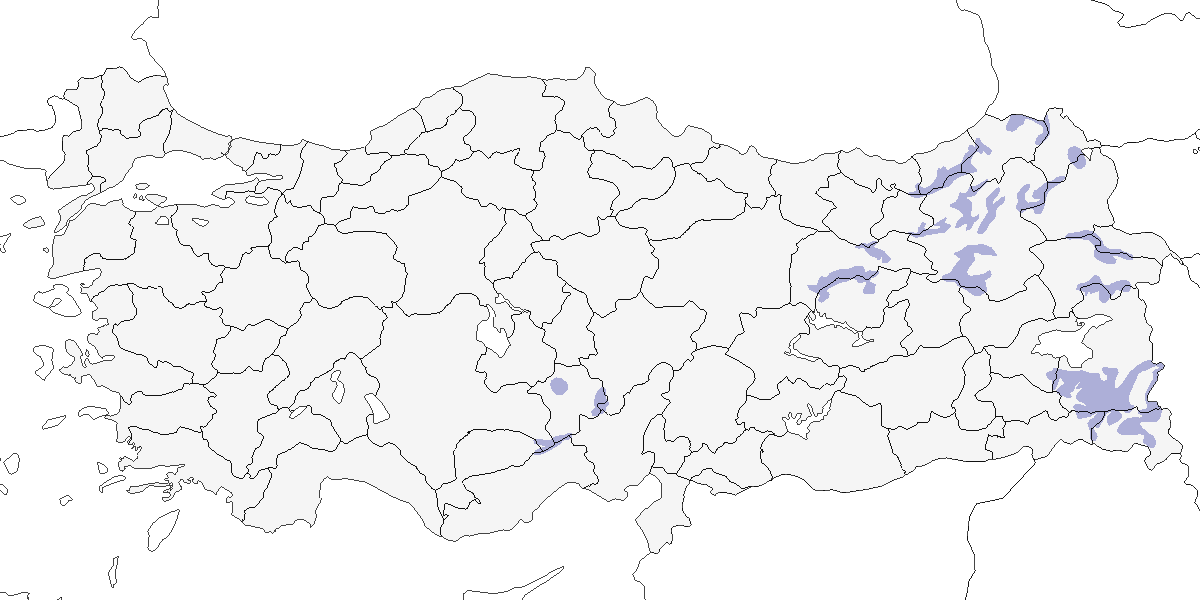
\includegraphics[keepaspectratio]{images/harita_Tetraogallus caspius.png}}

\textbf{Üreme}

\textbf{Yuvalama Alanı:} Özellikle 2400 metre üzerinde, alpine
çayırlarla kaplı, dik kayalıkların ve yarların olduğu, yıl boyunca karlı
bölgelerde ürerler.\\
\textbf{Yuvası:} Karanfil Dağı'nda 2100 metre yükseklikte 23 Nisan 1876
tarihinde, bir dişi çıkıntılı bir kaya ve ardıç kökü ile sarılmış bir
yuvanın bulunduğu dik bir su yolundaki küçük bir kaya üzerinden
uçmuştur. Yuva, taşlı toprak üzerinde derin yuvarlak bir oyuk olup
yetersiz düzeyde kuru otlar ve birkaç kuş tüyüyle astarlıdır. Bu yuvada
altı yumurta kaydedilmiştir. 25 Nisan 1876 tarihinde Bolkar
Dağları'ndaki iki yuva benzer özelliklerde kaydedilmiştir. Ancak bir
tanesi yeşil köknar ibreleri ile astarlanmıştır.\\
\textbf{Yumurta sayısı:} Yukarıdaki üç yuvada altı ve dört yumurta
kaydedilmiştir. İki yumurta Manchester Müzesi'nde, diğerleri ise Tring
Doğa Tarihi Müzesi'nde saklanmaktadır.\\
\textbf{Üreme dönemi:} \textbf{KAR:} Sivrikaya'da (Rize) beş genç ile
bir ergin 12 Haziran 1989 tarihinde küçük karlı alanları geçerken
kaydedilmiştir. \textbf{AKD:} Nisan 1876 tarihinde Toroslar Aladağlar
bölgesindeki yuvaları araştırmıştır (Danford, 1877-78) . 8 Temmuz 1986
tarihinde Aladağlar'da 1-2 haftalık 5 genç ile bir ergin gözlenmiştir.
İlk yumurta 21 Mayıs tarihinde bırakılmış olmalıdır. Çil Keklik
büyüklüğünde 5-6 ferik ile bir dişi 3-5 Ağustos 1967 tarihinde
kaydedilmiştir (Vielliard, 1968). 19 Ağustos 2000 tarihinde, bazıları
erginlerden belirgin derecede küçük 3-4 ferikli en azından üç aile grubu
kaydedilmiştir.

Ermenistan'da ortalama yumurtlama dönemi 10-15 Mayıs, kuluçka dönemi ise
20-30 Mayıs arasındadır. Yavrular 13 Haziran tarihinde kaydedilmiştir
(Adamian \& Klem, 1999). Gençlere ait bazı erken kayıtlar ilk yumurtanın
23 Nisan veya öncesinde bırakıldığını ortaya koymaktadır. Nisan sonu ile
mayıs başını içeren iki kayıt Danford'un Türkiye'de kaydettiği yuva
tarihleri ile kabaca uyum göstermektedir.

\textbf{Alttürler ve Sınıflandırma}

Monotipik bir türdür. Eskiden Hakkari ve Zagros Dağları'ndaki kuşların
\emph{semenowtianschanskii} (Zarudny, 1908), Toros Dağları'ndaki
kuşların \emph{tauricus} (Dresser, 1876) ve Erzurum bölgesindeki
kuşların \emph{challayei} isimli ayrı alttürler olduğu düşünülmüştür.

\section{Kum Kekliği}\label{kum-kekliux11fi}

\emph{Ammoperdix griseogularis}, See-see Partridge

\textbf{\emph{Güneydoğu Anadolu'da yaygın olarak çok sayıda bulunan
yerli türdür.}}

İlk zamanlarda çoğunlukla Suriye sınırına 50 km mesafedeki 15
lokaliteden bilinirdi. Ancak, Güneydoğu Anadolu'da yürütülen kapsamlı
bir biyoçeşitlilik araştırması, uygun habitatların bulunduğu alanlarla
birlikte türün hemen hemen 50 coğrafi yerde bulunduğunu göstermiştir
(Zeydanlı \emph{vd.}, 2005). Çoğunlukla az sayıda gözlenir, ancak
sonbaharda 40 bireylik gruplar kaydedilmiştir.

\pandocbounded{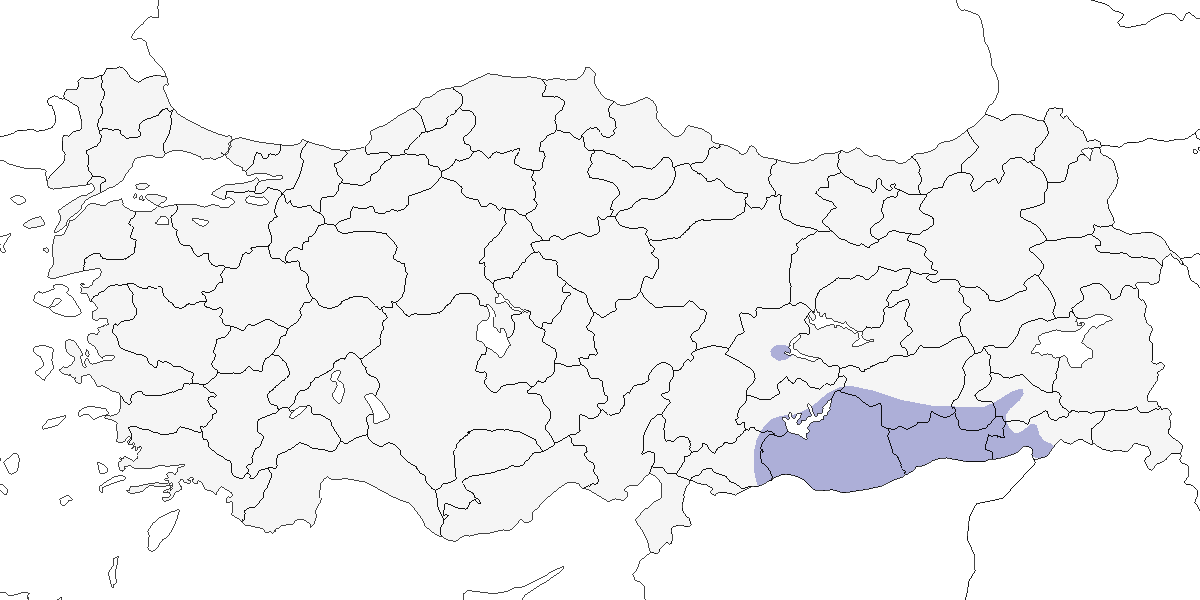
\includegraphics[keepaspectratio]{images/harita_Ammoperdix griseogularis.png}}

\textbf{Üreme}

\textbf{Yuvalama Alanı:} Güneydoğu Anadolu'da zayıf vejetasyon örtüsüne
sahip kurak kayalık alanlarda üremektedir.\\
\textbf{Yuvası:} Türkiye içerisinde yuva ve yumurta tanımlaması
yapılmamıştır; ancak, diğer yerlerde yuvalar, yuvanın bulunduğu yere
yakın bitki materyalleri ve otlarla astarlanmış, genellikle taş ya da
bir tutam bitki ile çevrelenmiş şekilde zeminde, toprağa kazılmış halde
bulunur.\\
\textbf{Yumurta sayısı:} Kuluçka küme büyüklüğü genellikle 8-12
arasındadır, bazen yumurta sayısı 16'ya kadar çıkabilmektedir.\\
\textbf{Üreme dönemi:} Nisan ayında çiftler kaydedilmiştir. 5-7 Haziran
1973 tarihinde Halfeti'de kaydedilen üç haftalık üç genç birey ile bir
ergin, diğer yerlerde kaydedilen ilk yumurtayı koyma tarihiyle
çelişmeyecek şekilde ilk yumurtaların nisan ortasında bırakıldığını
göstermektedir. 2004-05 yıllarında Birecik'te birkaç genç birey
kaydedilmiştir. 11 Ağustos 2001 tarihinde Cizre'de bir aile kaydedilmiş,
gençlerin boyu hakkında detaylar verilmemiştir.

\textbf{Alttürler ve Sınıflandırma}

Monotipik bir türdür.

\section{Bıldırcın}\label{bux131ldux131rcux131n}

\emph{Coturnix coturnix}, Common Quail

\textbf{\emph{Yaygın olarak çok sayıda bulunan bir yaz konuğu ve geçit
türüdür. Nadiren az sayıda kışlar.}}

Çoğunlukla tahıl ekilen kurak tarlalar, bozkırlar, çayırlar ve yüksek
otların bulunduğu dağlık bölgelerin yanında yoğun vejetasyonlu kumullar
gibi alanlarda bulunur. Özellikle İç Anadolu'da oldukça yaygın olarak
ürer, ancak hububat tarımının nispeten az olduğu kıyısal bölgelerde
oldukça azdır. Doğu kesimlerinden en azından 2300 metreye kadar
üreyebilir. Üreme ve geçit sırasında özellikle tahıl ekilen arazilerde
bulunur.

Üreme dışında, geçit sırasında tüm ülkede bol sayıda bulunur. İlkbahar
geçişi mart sonu ve nisan arasında, sonbahar geçişi ise ağustos sonu ve
eylül boyunca, hatta kuzey bölgelerinde daha erken gerçekleşir. İlkbahar
göçünde kuzey bölgelere mart sonu itibariyle ulaşır. Sonbahar göçünde
Karadeniz kıyılarında kasıma kadar göçünün sürdüğü bilinir (Albrecht,
1986). Kasım sonunda, 26 Kasım 2003'te Seyfe Gölü'nde ve 20 Kasım
2010'da Nallıhan Kuş Cenneti'nde kaydedilmiştir (Balmer \& Betton,
2004a). Az sayıda Ege ve Akdeniz kıyılarında kışlar, bu durum geçişin
sonunun tespitini zorlaştırır.

Tarım arazilerinde yaşayan diğer kuşlar gibi, tarımın yoğunlaşması,
tahıl dışındaki ürünlerin çoğalması ve yasadışı avcılık sonucunda
sayıları ülke çapında azalmıştır. Göçmen kuşlar aşırı av baskısı
altındadır ve özellikle Karadeniz bölgesinde yasadışı teyp kullanarak
yakalama faaliyetleri devam etmektedir.

\pandocbounded{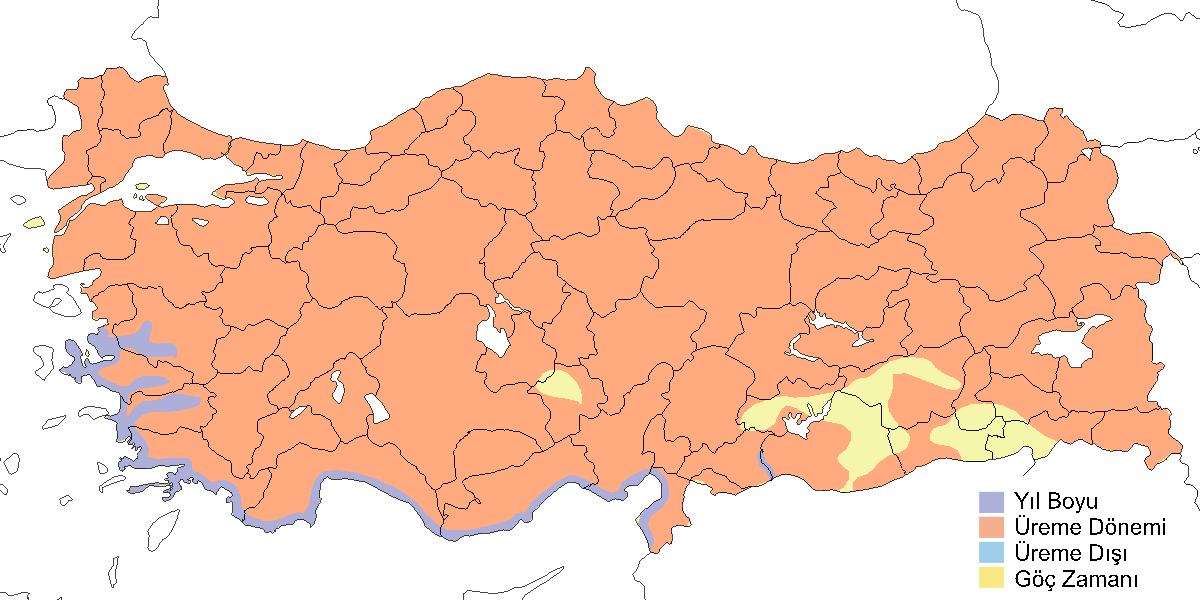
\includegraphics[keepaspectratio]{images/harita_Coturnix coturnix.png}}

\textbf{Üreme}

\textbf{Yuvalama Alanı:} Özellikle hububat tarlalarında yuvalar.\\
\textbf{Yuvası:} Ürediğini kanıtlamak son derece zordur ve Türkiye'de
henüz bir yuvası tespit edilmemiştir. Türkiye dışında, yerdeki düzce bir
çukuru ot ve yakındaki bitkisel materyal ile astarlar.\\
\textbf{Yumurta sayısı:} Genellikle 7-12, istisnai olarak 6-18 arasında
yumurta koyar.\\
\textbf{Üreme dönemi:} Genellikle nisan sonu ile mayıs ortası arasında
yumurta koyar. \textbf{MAR:} Uluabat Gölü'nde 22 Mayıs 1966'da yavrular
gözlenmiştir. Çoğu bölgeye ilkbaharda nisan ortasından gelir ve tüm
yavru gözlemleri üremenin alana varıştan hemen sonra başladığını
gösterir. Ağustos'ta duyulan kuşlar gecikmiş bir üremenin göstergesi
olabilir. \textbf{GDA:} Birecik'te 4 Haziran 1993'te tamamen palazlanmış
3 haftalık 9 yavru, hasat döneminde biçilmiş mısırın altında saklanırken
görülmüş ve köylüler tarafından yenmek üzere yakalanmıştır. 5 Haziran
1993'te görülen başka 6 kuş, yumurtlama tarihinin yaklaşık 20 Nisan'da
olduğunu gösterir. Suriye'de yavrularıyla dolaşan bir çift temmuz ayında
gözlenmiştir (Baumgart \emph{vd.}, 1995).

\textbf{Alttürler ve Sınıflandırma}

Türkiye'de nominat alttürü bulunur.

\section{Kınalı Keklik}\label{kux131nalux131-keklik}

\emph{Alectoris chukar}, Chukar Partridge

\textbf{\emph{Yaygın olarak çok sayıda bulunabilen bir yerli türdür.}}

Yaygın, Trakya ve Batı Karadeniz kıyı şeridinde nadir, Türkiye genelinde
ise oldukça bol bulunan yerli bir kuş türüdür. İç bölgelerde genellikle
700-2000 metre arasında görülür ve genellikle kurak, kayalık tepe ve
dağlık alanlarda, en az 2800 metreye kadar kaydedilmiştir. Hemen hemen
40 bireye kadar çıkabilen ve gençleri de içeren oldukça büyük sürüler
gözlenmiştir.

Geçmişte özellikle Hatay ve Doğu Karadeniz kıyı şeridi gibi bölgelerde
oldukça bol olarak kaydedilmiş, ancak son zamanlarda belirgin bir azalma
göstermiştir.

\pandocbounded{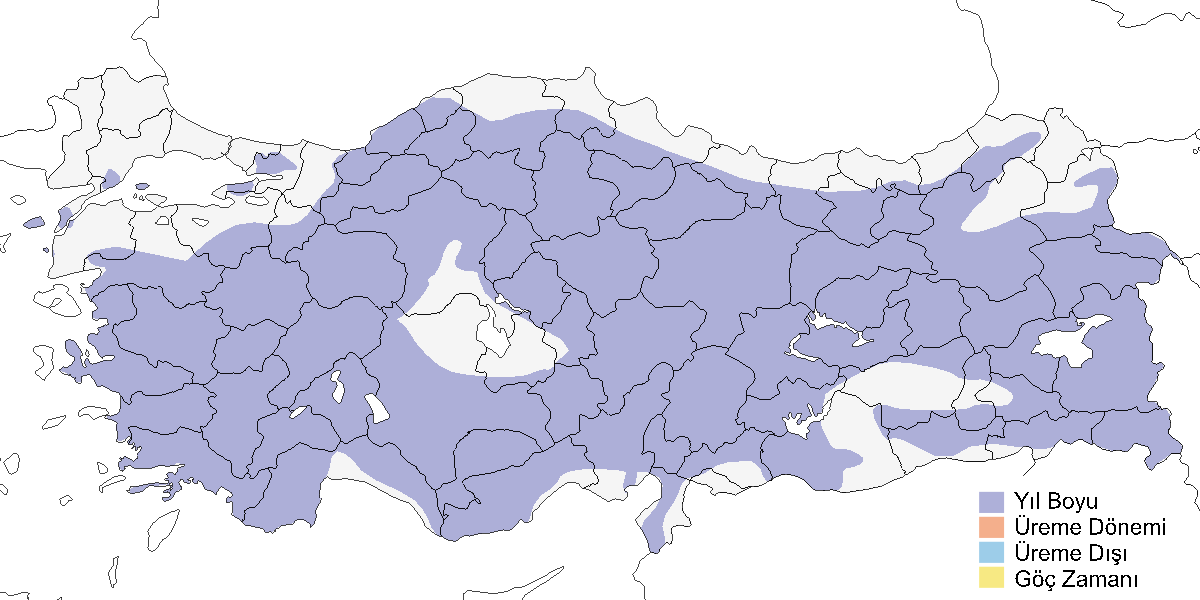
\includegraphics[keepaspectratio]{images/harita_Alectoris chukar.png}}

\textbf{Üreme}

\textbf{Yuvalama Alanı:} Bodur çalılar ile kurumuş tarım alanlarının
bulunduğu kayalık ve taşlık tepelerle oldukça kurak ve çorak alanlarda
ürer.\\
\textbf{Yuvası:} Yerde yuvasını bir çalı ya da bitki dibine gizler.\\
\textbf{Yumurta sayısı:} Genellikle 5-22 arasında değişmekle birlikte,
bazı bölgelerde daha düşük ya da yüksek sayılarda yumurta
kaydedilmiştir.\\
\textbf{Üreme dönemi:} Genellikle mayıs sonu ile haziran başı arasında
yumurtlamaya başlar. Yavrular, temmuz ayı ortasına kadar
gözlemlenebilir. Farklı bölgelerde kaydedilen üreme dönemleri, ortam
koşullarına bağlı olarak değişiklik gösterebilir. \textbf{EGE:}
Kuluçkadaki bir ergin birey, İzmir yakınlarında 14 yumurta içeren bir
yuvadan (Ramsay, 1914) 7 Mayıs 1951 tarihinde alınmıştır. Yuva, yuvanın
sahibi olan kuşun çok sayıda tüyü ile birlikte çalı benzeri bitkilerle
astarlanmış ve dikenli meşe ile de korunmuştur. Yumurtalar krem ile
kırmızı arasında bir renklenme ile kırmızımsı küçük beneklenmeler
gösterir (McNeile, 1950, 1951, 1954, 1967, 1968, 1970, 1972, 1973).
\textbf{AKD:} 11 Mayıs 1899 tarihinde Acıgöl'de 5 yumurtalı bir yuva
kaydedilmiştir; dişinin yumurtlamaya devam edeceği düşünülmüştür
(Selous, 1900). Karadağ'da, taze yumurtalar içeren iki yuva 1907 yılının
Mayıs sonunda kaydedilmiştir. Bu yuvada taze yumurtalar haziran ayında
da bulunmuştur. Bir ergin ile 5-6 iyi gelişmiş genç birey, Burdur ve
Bucak arasındaki geçitte 13 Temmuz 1968 tarihinde kaydedilmiştir
(Rokitansky \& Schifter, 1971). \textbf{İÇA:} 22 yumurta içeren bir
yuva, 24 Mayıs 1998 tarihinde Ereğli yakınlarındaki bir kraterin, bir
çalı ile sarılmış kaya çıkıntısı üzerinde kaydedilmiştir. 20 yumurtadan
9 tanesi nisan ayı sonunda bırakılmıştır (Banoğlu ve Burr 1953).
\textbf{DOA:} Nemrut Dağı'nda (Bitlis), 9 Haziran 2004 tarihinde sabah
saatlerinde 15 yumurtalı bir yuva kaydedilmiştir. Ancak, günün ilerleyen
saatlerinde, ergin bir birey yuva üzerine oturmuştur. Muhtemelen bu
tarih inkübasyonun ilk günü olarak belirtilebilir. Yuva, kısmen yaprak
döken ormandaki bodur çalılar altında bulunur. Zemine derin bir şekilde
kazılmış ve birkaç adet ergin kuş tüyü ve otların kökleri ile
astarlanmıştır. \textbf{GDA:} Kuluçka kayıtları 2 Haziran 2001 tarihinde
Işıklı'da (Gaziantep) gençleri içermektedir ve 22 Haziran 1966 tarihinde
Menemen (İzmir) yakınlarında 6, 7 ve 8 yavrulu bireyleri içermektedir.
Akdeniz Bölgesi'nde 22 Mayıs 1989 tarihinde bir kuluçka ve 30 Haziran
1966'da Aladağlar'da birkaç günlük genç bir birey kaydedilmiştir. Birkaç
kuluçkanın birleşmesi sonucunda oluşan ve yaygın olarak gözlemlenmeyen
büyük kuluçkalar, tek bir ergin ile birlikte 13 Ağustos 1967 tarihinde
Kızılcahamam'da (Ankara) kaydedilmiştir (Barış, Akçakaya \& Bilgin,
1984).

\textbf{Alttürler ve Sınıflandırma}

Türkiye'nin güneyi boyunca \emph{cypriotes} alttürü görülmektedir.
Kuzeyde \emph{kleini} ve Doğu Akdeniz bölgesine özgü \emph{sinaica}
alttürünün etkili olduğu bölgede, Güneydoğu Anadolu'da
\emph{kurdestanica} alttürü bulunmaktadır. Tür içerisindeki coğrafi
varyasyon konusu ile ilgili kesin bir çıkarım yapılamamıştır; ancak
gözlemlenen formların tamamı, güçlü bir şekilde gradient ile birlikte
belirgin klinal yapı göstermektedir (Madge \& McGowan, 2002).

\section{Kaya Güvercini}\label{kaya-guxfcvercini}

\emph{Columba livia}, Rock Dove

\textbf{\emph{Menşei karışık olarak; yaygın ve çok sayıda bulunan
yerlidir.}}

Şehir güvercini formunda ülke çapında ve özellikle İstanbul, İç Doğu ve
Güneydoğu Anadolu'da yaygın ve çok boldur. Saf veya safa yakın kaya
güvercini formu çok daha az sayıda bulunur ve güneyde 3000 m. kuzeyde ve
doğudan 4000 metreye kadar yükseklikteki kayalık ve dağlık arazide ve
deniz kıyısındaki yarlarda bulunur. Saf popülasyonların tespit
edilebilmesi için gözlemcilerin yabani dondaki güvercin gruplarını daha
ayrıntılı tanımlamaları gerekmektedir. Buna rağmen en azından Güneydoğu
Anadolu'da şehir kuşları ve insan yerleşimlerine yakın üreyebilen yabani
kuşları birbirinden ayırt etmek mümkün görünmemektedir.

\pandocbounded{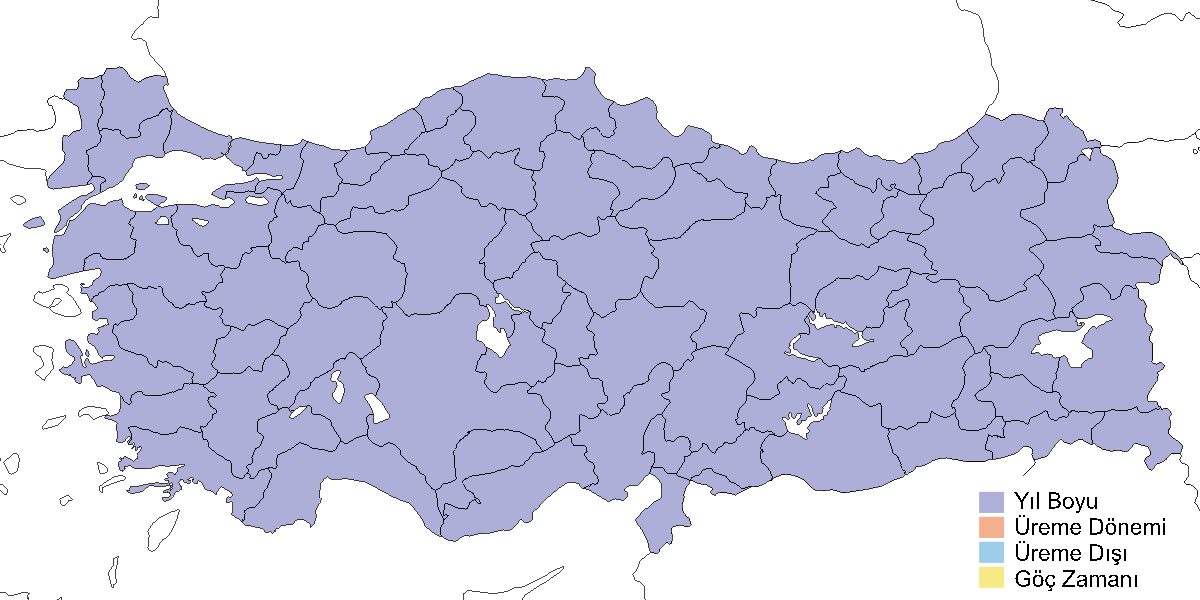
\includegraphics[keepaspectratio]{images/harita_Columba livia.png}}

\textbf{Üreme}

\textbf{Yuvalama Alanı:} Çoğunlukla 20 çiftten az küçük koloniler
halinde, bazen de tek başına yuvalar. Kaya oyukları, yarlardaki
mağaralar, serpme kaya yığınları, binalar, harabeler, yer kuyuları ve
yerde çalıların altına yuva yapar. Bazen yuvalama alanını diğer
kuşlarla, özellikle küçük karga ile paylaşır.\\
\textbf{Yuvası:} Dallardan, ince bitki gövdelerinden ve köklerden oluşan
ince bir platformdur.\\
\textbf{Yumurta sayısı:} 15 yuvada 2 yumurta, olası tamamlanmamış
kuluçkalarda ise 2 yuvada 1 yumurta kaydedilmiştir. İki yuvada ikişer
yavru görülmüştür.\\
\textbf{Üreme dönemi:} Şehir güvercini muhtemelen yıl boyu yuvalar. Kaya
güvercini mart ayından itibaren yumurta koyar, yavrular mayıs sonu
yuvadan ayrılır. \textbf{EGE:} 8 Mayıs 1950'de Çeşme açıklarındaki Ilıca
Adası'nda, düz bir zeminde bir çalının altında içinde uzun süredir
kuluçkaya yatılan iki yumurta olan bir yuva görülmüştür (McNeile, 1950,
1951, 1954, 1967, 1968, 1970, 1972, 1973). 14 Mayıs 1899'da, İzmir
yakınlarındaki bir harabede içinde iki yumurta bulunan bir yuva
kaydedilmiştir (Selous, 1900). \textbf{İÇA:} 22 Mayıs 2007'de aynı
yuvada hem tam gelişmiş iki yavru hem de iki yumurta görülmüştür
(Ramsay, 1914). Bunun, iki çiftin üremesinden kaynaklandığı ve
muhtemelen yavruların kendi yuvalarından ayrıldığı düşünülmüştür. 7
Mayıs'ta görülen yeni palazlanmış yavru, yumurtlamanın mart ortasında
başladığını göstermektedir. Bolluk Gölü'ndeki bir adada bulunan
kolonide, kuşlar yerde çalıların altında suna yuvalarıyla karışık olarak
yuvalamışlardır. Hem 24 Haziran 1992'de hem de 7 Mayıs 1993'te yaklaşık
5 yuvada ikişer yumurta görülmüş olup, bu durum türün yılda iki kez
kuluçkaya yattığını açıkça göstermektedir. \textbf{DOA:} 9 Haziran
2001'de Balık Gölü'nde birçok çift, küçük karga ile birlikte gölün
ortasındaki bir adadaki kaya yığınları arasında yuvalamıştır.

\textbf{Alttürler ve Sınıflandırma}

Türkiye' genelinde nominat alttür bulunur. Bunun yanında (Kumerloeve,
1961) kuzeydoğuda gaddi alttürü ve güneyde \emph{palaestinae} alttürü
olduğunu düşünmüş, Roselaar (Cramp, 1985) Türkiye ve Kafkas
popülasyonları için ayrı bir alttür tanınması önermiştir.

\section{Gökçe Güvercin}\label{guxf6kuxe7e-guxfcvercin}

\emph{Columba oenas}, Stock Dove

\textbf{\emph{Seyrek ve lokal yaz konuğu, nispeten yaygın ve az sayıda
geçit kuşu ve kış konuğudur.}}

Ülkenin zengin ormanlı dağlık bölgelerinde en azından 2100 metreye kadar
çıkan oldukça az sayıda ve yerel dağılım gösteren yerli ve yarı
göçmendir. Istranca Dağları'nda büyük ihtimalle üremektedir, Mayıs,
Ağustos 2009 arasında yapılan çalışmada bazı ihtimaller gözlenmiştir
(Özkan 2010). Bulgaristan tarafından ürediği bilindiği için büyük bir
sürpriz değildi (Milchev, 1994). Doğu Karadeniz'in bazı bölgelerinde 400
metrenin altında nispeten bol olarak ürer (Faldborg, 1994). Geçit
sırasında daha yaygındır. İstanbul Boğazı'ndan Eylül ortası ile Ekim
sonu arasında en yüksek sayıda da Ekim ortasında geçit yapar (Porter,
1983; Beaman, 1986). Kuzeydoğu Anadolu'da en yüksek sayılarda Ekim
ortası ile sonu arasında geçer (Beaman, 1986). İlkbaharda geçişinde
Kızılırmak Deltası'nda Mart sonu en yoğun geçer ve geçişi nisan ortasına
kadar geçtiği saptanmış olsa da (Hustings \& Dijk, 1994), bu yayındaki
çalışma muhtemelen erken göçünü kaçırmıştır. Sonbahar göçünde güney
kıyılarında ve hatta doğu bölgelerinde de bulunabilir. Kışın batı ve
orta bölgelerinde özellikle İç Anadolu'nun batı, güneybatı ve güney
kısımlarında Toros Dağları eteklerinde yer yer kayda değer sayılarda
olabilir. Üremeyen kuşlar kışlama alanlarında Mayıs ortasına kadar
kalabilir.

\pandocbounded{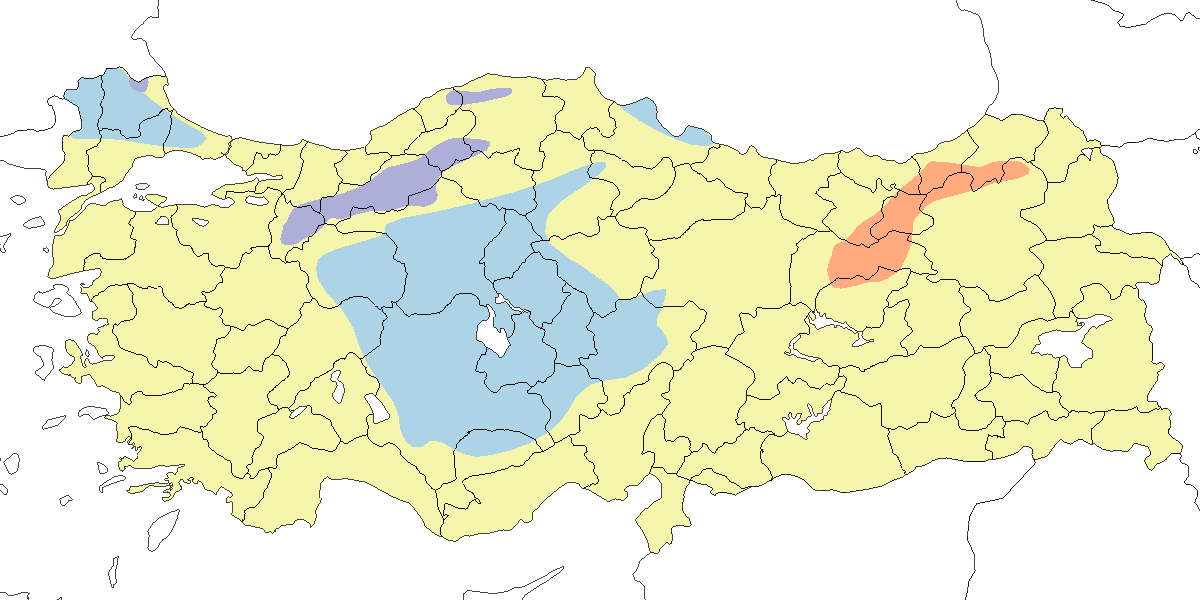
\includegraphics[keepaspectratio]{images/harita_Columba oenas.png}}

\textbf{Üreme}

\textbf{Yuvalama Alanı:} Bir bilgi yoktur.\\
\textbf{Yuvası:} Bir bilgi yoktur.\\
\textbf{Yumurta sayısı:} Türkiye'den bir bilgi yoktur. Muhtemelen 2
yumurta koyar.\\
\textbf{Üreme dönemi:} Bir bilgi yoktur.

\textbf{Alttürler ve Sınıflandırma}

Türkiye'de nominat alttürü bulunur.

\section{Tahtalı}\label{tahtalux131}

\emph{Columba palumbus}, Common Wood Pigeon

\textbf{\emph{Oldukça yaygın ve nispeten çok sayıda bulunan yerli ve
yarı göçmen, yaygın ve çok sayıda bulunan geçit türü ve kış konuğudur.}}

Akdeniz Bölgesi'nde en yaygın, İç Anadolu'da seyrektir. Genellikle daha
kurak ve çoğunlukla dağlık ibreli ormanlarda ürer, yayılışı seyrek
olabilir. Deniz seviyesinde az sayıda ürer, çoğunlukla 900 metrenin
üstündedir, en azından 2200 metreye kadar çıkabilir.

Ülke çapında geçit sırasında daha yaygındır, İstanbul Boğazı'ndan geçişi
eylül başından ekim başı arasında, dolayısıyla gökçe güvercinden daha
erkendir. 2-4 Ekim 1974'te 647 tane sayılmış, 24 Eylül ve 8 Ekim 1973'de
de toplam 11.780 kuş sayılmış, en yoğun geçiş 2000 kuşla 2 Ekim'de
gerçekleşmiştir. Göçü güney kıyılarında da hissedilir, ancak
Akdeniz'deki büyük nehir deltalarında çok seyrektir. Marmara ve İç
Anadolu'nun iç bölgelerinde göç sırasında birkaç yüzlük sürüler halinde
görülebilir. Kışın yer yer yüksek sayılarda görülebilir, İç Anadolu'da
genellikle azdır. Batı ve güneyde kışlayan sürüler iç bölgelerden göç
alabilir, Aralık 1969'da Antalya Korkuteli'nde 950, Burdur Gölü'nde
740'lık sürülere rastlanmıştır. İlkbahar göçü mart ortası ve nisan
ortası arasında yoğunlaşır, 24-31 Mart 1972'de Manyas Kuşcenneti'nde
toplanan yaklaşık 10.000, 19 Kasım 2005'te Sandıklı ve Afyon arasında
toplanan 2000 kuş ve Aralık 2004'te Meriç Deltası'nda toplanan
binlercesi son derece istisnai bir kalabalık oluşturmuştur. Kışlama
alanlarında mayısın ilk haftasına kadar kalabilir.

\pandocbounded{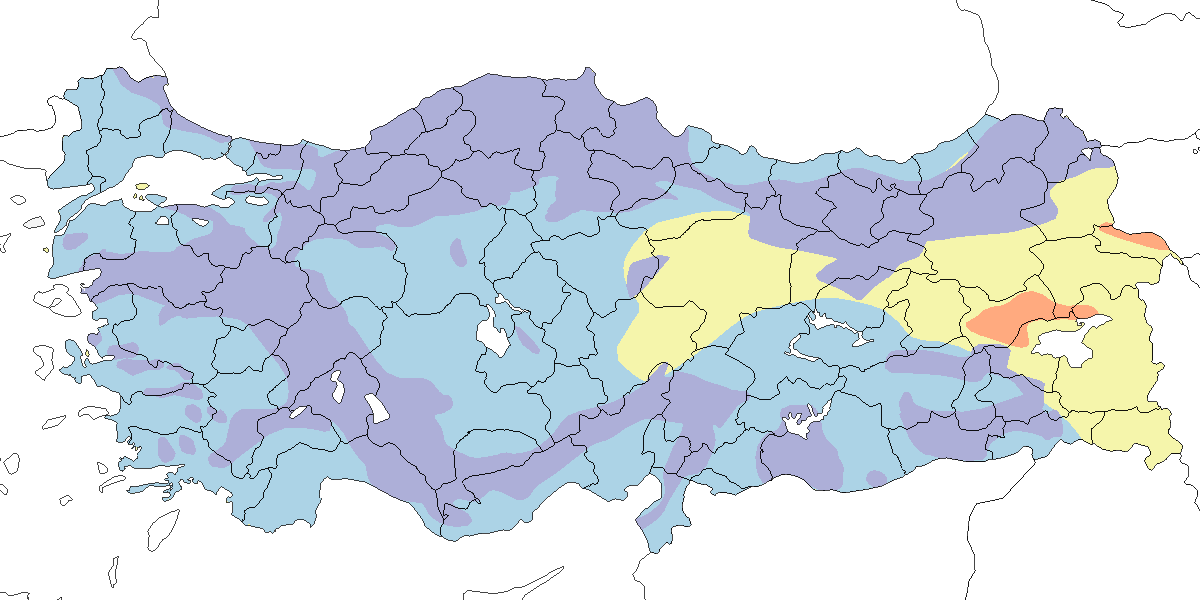
\includegraphics[keepaspectratio]{images/harita_Columba palumbus.png}}

\textbf{Üreme}

\textbf{Yuvalama Alanı:} Çam ormanları, meyvelik bahçeler ve nehir
boyundaki riperyan alanlarda yuvalar.\\
\textbf{Yuvası:} Türkiye'den bir bilgi yoktur.\\
\textbf{Yumurta sayısı:} Türkiye'den bir bilgi yoktur. Muhtemelen 2
yumurta koyar.\\
\textbf{Üreme dönemi:} Nisan ve mayısta gösteri uçuşu yaptığı gözlenmiş,
yumurta koyduğu varsayılmıştır. Yavrular mayıstan itibaren görülür.
\textbf{KAR:} Nisan 1992'de, Kızılırmak Deltası Yörükler Ormanı'nda bazı
bireylerin gösteri uçuşu yaptığı kaydedilmiştir. 3 Haziran 1992'de yuva
yakınında bir kuş görülmüştür (Hustings \& Dijk, 1994). 16 Haziran
1975'te, Zigana Dağı Torul yakınlarında genç bireyler gözlenmiştir.
\textbf{GDA:} 3 Mayıs 2004'te, Gaziantep Karkamış'ta gösteri uçuşu
gözlenmiştir.

\textbf{Alttürler ve Sınıflandırma}

Türkiye'de nominat alttürü bulunur (Roselaar, 1995). Güneydoğu'da
\emph{iranica} alttürü ile bir geçişin görülebilir olduğundan bahseder.
Doğuda \emph{iranica} alttürünün \emph{casiotis} alttürüne geçiş
yaptığından dolayı \emph{iranica} \emph{casiotis} alttürünün bir
sinonimi olabilir (Gibbs, Barnes \& Cox, 2001).

\section{Üveyik}\label{uxfcveyik}

\emph{Streptopelia turtur}, European Turtle Dove

\textbf{\emph{Yaygın ve yer yer çok çok sayıda bulunan yaz konuğu ve
geçit türüdür.}}

Ülkenin çoğu yerindeki ormanlık ve tarımsal arazilerde genellikle
oldukça çok ve yaygın olan bir yaz konuğudur. Batıda daha yaygın, doğuda
da oldukça lokaldir. Kızılırmak Deltası'nda 1992'de toplam 600-800
çiftin ürediği tahmin edilmiştir (Hustings \& Dijk, 1994).Karadeniz ve
Marmara bölgelerinde 1500 metreye kadar, Toroslar'da 200-1300 metrede,
Kuzeydoğu Anadolu'da da 2000 metreye kadar yuvalar. Geçit sırasında daha
yaygındır, sıka çok yüksek sayılarda görülür. İlkbaharda nisan başında
gelir, ekim başına kadar kalır. İstanbul Boğazı'ndan ciddi ölçekte bir
geçiş olmasa da Kuzeydoğu Anadolu ve kısmen Doğu Anadolu'da çok bol
sayıda görülür. 1968 Eylül sonunda yüzlercesi Silifke ve Antalya
arasındaki Akdeniz kıyısında gözlenmiş, yaklaşık 1000 tanesi 16 Haziran
1975'te Zigana Geçidi ve Trabzon arasında, aynı tarihte yaklaşık
3000-4000 tanesi Erzurum ve Gümüşhane arasında, yaklaşık 2000 tanesi 2
Mayıs 2004'te Birecik'in güneyinde gecelerken gözlenmiştir. İlkbahar
geçişi az ölçekte de olsa özellikle kuzey bölgelerinde haziran ortasında
kadar devam eder. En erken geliş tarihi 30 Mart'tır. Dönüş temmuzun son
haftasında başlar, eylül ayında tepe yapar ve genellikle ekim başında
biter. İç Anadolu'da en geç 28 Ekim'de görülmüştür.

\pandocbounded{\includegraphics[keepaspectratio]{images/harita_Streptopelia turtur.png}}

\textbf{Üreme}

\textbf{Yuvalama Alanı:} Ağaçlık, çitlik ve yüksek çalıların bulunduğu
doğal ve tarımsal arazilerde, meyve ve zeytin bahçelerinde, ormanlarda
ve orman kenarlarında ürer.\\
\textbf{Yuvası:} Genellikle bir çalıya veya alçak bir ağaca, yerden 2-4
metre yukarıya yapılır. İnce dallardan örülmüş sığ bir platform olup,
hafif çukur ortası otlar ve ince köklerle astarlanır.\\
\textbf{Yumurta sayısı:} On üç yuvada 2 yumurta, bir yuvada ise 1
yumurta kaydedilmiştir. Üç yuvada 2 yavru gözlenmiştir.\\
\textbf{Üreme dönemi:} Mayıs ayından itibaren yumurta koyar. yavrular
temmuzda görülür. Türkiye dışında yılda iki hatta üç kez kuluçkaya
yattığı ve üremenin ağustosa kadar devam ettiği bilinmektedir. Ancak,
Türkiye'den henüz böyle bir gözlem kaydedilmemiştir. \textbf{EGE:} 10
Mayıs 1950'de, içinde yeni konmuş yumurtalar bulunan bir yuva en erken
üreme kaydıdır (McNeile, 1950, 1951, 1954, 1967, 1968, 1970, 1972,
1973). İzmir ve Aydın Akköy'de mayısın ikinci yarısı ve haziran başında
birkaç başka kayıt bulunmaktadır. 24 Haziran 1966'da, Bafa Gölü'nde
içinde iki yumurta bulunan bir yuva gözlenmiştir. \textbf{KAR:}
Kızılırmak Deltası'nda, Temmuz 1971'de 1 hektarlık ormanda sekiz tane
kullanılan yuva sayılmıştır (Dijksen \& Kasparek, 1985). \textbf{İÇA:}
30 Mayıs 1999'da, Göreme yakınlarında dört erişkin gösteri uçuşunda
gözlenmiştir. 25 Haziran 1992'de, Hasan Dağı'nda içinde bir ve iki
yumurta bulunan ve muhtemelen ikinci kez kuluçkaya yatılan iki yuva
bulunmuştur. Ancak, 13 Haziran 1907'de Karaman Karadağ'da içinde birkaç
günlük iki yavru bulunan bir yuva kaydedilmiştir (Ramsay, 1914), bu
kaydın muhtemelen ilk kuluçkaya ait olduğu düşünülmektedir.
\textbf{GDA:} 18 Mayıs 1993'te, Birecik'te içinde iki yumurta bulunan
bir yuva bulunmuştur. 11 Mayıs 2004'te, Halfeti'de küçük bir meyve
bahçesinde 1,7 metre boyundaki ağaçlarda ikişer yumurta bulunan iki yuva
kaydedilmiştir. 8 Haziran 1993'te, Gaziantep yakınlarında yuva kuran
erişkinler ve 14 Haziran 1996'da muhtemelen ikinci yuvayı kuran bireyler
gözlenmiştir.

\textbf{Alttürler ve Sınıflandırma}

Türkiye'de nominat alttürü bulunur.

\section{Büyük Üveyik}\label{buxfcyuxfck-uxfcveyik}

\emph{Streptopelia orientalis}, Oriental Turtle Dove

\textbf{\emph{Rastlantısal konuktur.}}

İlk kez 12-15 Ocak 2011 tarihlerinde Ayvalık'ta bir bahçede
kaydedilmiştir. İlk kışında olan ve diğer Avrupa ve Orta Doğu
kayıtlarıyla uyumlu olarak meena alttürüne ait olan ilk kışındaki bu
birey iyi şekilde fotoğraflanmıştır. Ardından aynı kış, 7 Şubat 2011'de
Yeşilırmak Deltası'nda bir birey gözlenmiş ve fotoğraflanmıştır.

\pandocbounded{\includegraphics[keepaspectratio]{images/harita_Streptopelia orientalis.png}}

\textbf{Üreme}

Türkiye'de yuvalamaz. Yayılış alanı Doğu Asya'dır.

\textbf{Alttürler ve Sınıflandırma}

Türkiye'de nominat alttürü bulunur. Tür bugünkü Türkiye sınırlarında
tanımlanmıştır.

\section{Kumru}\label{kumru}

\emph{Streptopelia decaocto}, Eurasian Collared Dove

\textbf{\emph{Yaygın ve çok sayıda bulunan yerli ve yarı göçmendir.}}

Genellikle alçak bölgelerde bulunur, Doğu Anadolu'da oldukça yerel
yayılış gösterir, Doğu Karadeniz'de yoktur. Son yıllarda hem Balkanlar
hem de Orta Doğu'da yayılış alanında ciddi değişimler yaşanmış ve bu
olgu (Kasparek, 1996a, 1998) tarafından incelenmiş ve Türkiye'yi de
içine alan bu coğrafyada yayılış alanındaki genişleme belgelenmiştir.
Bazı bölgelerde yarı göçmen olduğu düşünülür, kışları sert geçen iç
bölgelerde kıyı bölgelerine bir hareket vardır. Kışın ve ilkbaharda
yüzlerce kuştan oluşan sürüler gözlenmiştir. İstanbul ve diğer
metropollerde küçük kumru ile rekabet edememiş ve yerini küçük kumruya
bırakmıştır.

\pandocbounded{\includegraphics[keepaspectratio]{images/harita_Streptopelia decaocto.png}}

\textbf{Üreme}

\textbf{Yuvalama Alanı:} Tarım arazileri ve kentsel bölgelerde,
özellikle köy ve kasabalarda yuvalar. İdeal koşullarda, yapraklı ve
ibreli ağaçların karışık bulunduğu gelişmiş bahçe ve parklarda da ürer.
Yuvasını ağaçlara veya yüksek çalılara yapar. Bazen Mersin'de
gözlemlendiği gibi binalarda ve telefon direklerinde de yuvaladığı
kaydedilmiştir (Hollom, 1955).\\
\textbf{Yuvası:} İnce dal ve bitki gövdelerinden oluşan cılız bir
platformdur. Daha ince bitkisel materyaller ve diğer malzemelerle
özensizce astarlanır.\\
\textbf{Yumurta sayısı:} Üç yuvada ikişer yumurta sayılmıştır. İki
yuvada ikişer yavru gözlenmiştir.\\
\textbf{Üreme dönemi:} Genellikle nisan ve mayıs ayında ilk yumurtaları
koyar. Türkiye'de ve diğer bölgelerde yılda iki kez kuluçkaya yatar.
\textbf{EGE:} 23 Nisan 2003'te Aydın Akköy'de ve 9 Mayıs 1950'de
İzmir'de kuluçkadaki erişkinler gözlenmiştir (McNeile, 1950, 1951, 1954,
1967, 1968, 1970, 1972, 1973). 2 Haziran 1954'te İzmir'de bir yuvada
yeni bırakılmış iki yumurta kaydedilmiştir (McNeile, 1950, 1951, 1954,
1967, 1968, 1970, 1972, 1973). 29 Haziran 1966'da Akhisar'da, bir tespih
ağacının üzerine yerleştirilmiş hasır bir sepetteki yuvada kuluçkaya
yatmış bir erişkin gözlenmiştir. \textbf{AKD:} 18 Mayıs 1951'de
Mersin'de bir erişkinin yuvasını astarladığı gözlenmiştir (Hollom,
1955). 3 Mayıs 1970'te İskenderun'da bir yüksek gerilim hattı direğine
yuva kuran bir erişkin gözlenmiştir. 5 Mayıs 2003'te Dalaman
Havaalanı'nda, bir sıra ibreli ağaçtaki yuvada kuluçkada bir erişkin
gözlenmiştir. 6 Mayıs 2004'te Göksu Deltası'nda iki erişkinin kuluçkada
olduğu iki yuva kaydedilmiştir. \textbf{İÇA:} 24 Nisan 1991'de Konya
Hotamış'ta bir yuva bulunmuştur (Kirwan, 1993b). Haziran 1991'in ilk
haftasında, Kayseri İncesu'da bir karaçamın içindeki yuvada iki yumurta
tespit edilmiştir (BD). 23 Nisan 2004'te Şereflikoçhisar'da yol
kenarındaki bir ağaçta kuluçkaya yatan bir erişkin gözlenmiştir. 15
Mayıs 2004'te Cihanbeyli'de bulunan bir yuvada yumurtadan yeni çıkmış
iki yavru gözlenmiştir. \textbf{GDA:} 11 Mayıs 2004'te Halfeti
yakınlarında yuva yapımı gözlenmiştir. 3 Haziran 1998'de Birecik'te iki
yuvada ikişer yumurta bulunmuş, 11 Mayıs 2004'te ise iki yumurta
kaydedilmiştir. 25 Haziran 2001'de Birecik'te, yuvadaki iki iri yavru
bir yılan tarafından yenmiştir.

\textbf{Alttürler ve Sınıflandırma}

Türkiye'de nominat alttürü bulunur. Tür bugünkü Türkiye sınırlarında
tanımlanmıştır.

\section{Küçük Kumru}\label{kuxfcuxe7uxfck-kumru}

\emph{Spilopelia senegalensis}, Laughing Dove

\textbf{\emph{Nispeten yaygın ve çok sayıda bulunan yerlidir.}}

Ülkedeki yayılış alanı ve durumu (Kasparek, 1991) tarafından ayrıntılı
bir araştırma konusu olarak ele alınmıştır. Güneydoğu Anadolu, Doğu
Akdeniz ve İstanbul çevresinde kasaba ve şehirlerde çok bol bulunan
yerli kuştur. İstanbul'da gelen kuşların menşei Tunus'tan getirilen
kuşlar olduğu düşünülür. Ayrıca tüm yurtta çok yerel olarak şehirlerde
rastlanabilir. Bazı yerleşimlerde rekabet halinde olduğu kumruyu egale
etmeyi başarırken, diğerlerinde kumru daha baskın çıkar. En yoğun olarak
görüldüğü şehirler İstanbul, Adana, Mersin, Adıyaman, Gaziantep, Urfa,
Mardin ve Diyarbakır'dır. Daha küçük sayılarda Antalya, Afyon, Ankara,
Samsun, Erzincan ve Malatya'da, tek tük İzmir, Çanakkale, Edirne,
Tekirdağ, Konya, Hakkâri ve Van'da bulunur.

\pandocbounded{\includegraphics[keepaspectratio]{images/harita_Spilopelia senegalensis.png}}

\textbf{Üreme}

\textbf{Yuvalama Alanı:} İstanbul ve diğer şehirlerde yerleşim
alanlarında, Doğu Akdeniz ve Güneydoğu Anadolu'da köyler ve tarım
arazilerinde bulunur.\\
\textbf{Yuvası:} Bir çalı, ağaç veya bina cephesine yuva yapar. Yuvası,
ince çalılardan yapılmış basit bir platform olup, otlar ve ince bitkisel
malzemelerle astarlanır. Aynı yuva, yıl içindeki birbirini takip eden
kuluçkalar için tekrar kullanılabilir. Yuvanın farklı tabakalardan
oluşan yapısı ve eski dışkı kalıntıları, bu olgunun göstergesi olarak
kabul edilmektedir.\\
\textbf{Yumurta sayısı:} Bir yuvada 2 yumurta gözlenmiştir.\\
\textbf{Yavru sayısı:} Bir yuvada 2 yavru kaydedilmiştir.\\
\textbf{Üreme dönemi:} İstanbul'da ve muhtemelen diğer ılıman ve sıcak
şehirlerde yıl boyu yuvaladığı düşünülür. Diğer yerlerde üreme şubat ve
mart arasında başlar. \textbf{MAR:} İstanbul'da, 28 Mart 1967'de
çiftleşen bir çift gözlenmiş, 22 Nisan 1970'te bir pencere pervazındaki
yuvada oturan bir çift görülmüş ve Temmuz 1968 sonunda yavrusu olan bir
çift kaydedilmiştir. \textbf{AKD:} 28 Mart 2000'de, Adana
Havaalanı'ndaki bir palmiyede bir çiftin yuvaladığı gözlenmiştir. 18
Mayıs 2004'te, Adana şehir merkezinde yeni palazlanmış bir yavru
görülmüştür. \textbf{GDA:} 3 Mayıs 1964'te, Birecik'te yuvalayan çoğu
çiftin yavrularını beslediği, ancak bir yuvada hâlâ iki yumurta
bulunduğu kaydedilmiştir (Warncke, 1964-\/-65). 11 Mayıs 2004'te,
Halfeti'de yeni uçmaya başlamış ancak hâlâ hav tüyleri görülebilen bir
yavrunun yaklaşık bir hafta önce yuvadan ayrıldığı belirlenmiştir. Yakın
bir noktada, yerden 4 metre yukarıda, oturulan bir evin dış cephesindeki
bir çıkıntıda yaklaşık 7 günlük iki yavru gözlenmiş ve yumurtlama tarihi
20 Nisan olarak hesaplanmıştır. Aynı yuvanın yıl içinde daha önce de
kullanıldığı ve üremenin şubat ve mart aylarında başladığı gözlenmiştir.

\textbf{Alttürler ve Sınıflandırma}

Alttür tayini için inceleme yapılmamıştır. İstanbul'a Tunus'tan
getirildiği düşünülen ve çevre bölgelere yayılan kuşlar
\emph{phoenicophila} alttürü olduğu düşünülür. Güneydoğu Anadolu'da ve
buradan diğer bölgelere yayılan kuşların nominat alttüre olduğunu iddia
etmiştir (Kasparek, 1991).

\section{Kap Kumrusu}\label{kap-kumrusu}

\emph{Oena capensis}, Namaqua Dove

\textbf{\emph{Türkiye'ye yeni yerleşen ve lokal olarak bulunan
yerlidir.}}

İlk kez Birecik'in kuzeyinde 23-24 Mayıs 2005'te bir dişi
fotoğraflanmıştır. Ardından birer tane 23 Mayıs 2008'de Sinop'ta, 13
Mayıs 2010'da Niğde Çukurbağ'da, 8 Haziran 2012'de Kozanlı Gökgöl'de, 24
Haziran 2012'de Birecik'te ve son olarak 8 Kasım 2014'te Milleyha
Antakya'da denizden gelen bir birey fotoğraflanmıştır. İsrail'de Arava
vadisinde 1961'den beri yerleşik bir popülasyonun olduğu bilinir
(Shirihai, 1996).

\pandocbounded{\includegraphics[keepaspectratio]{images/harita_Oena capensis.png}}

\textbf{Üreme}

\textbf{Yuvalama Alanı:} Kurak ve sıcak bölgelerde bulunur. Muhtemelen
Çukurova ve Şanlıurfa'da yuvalamıştır.\\
\textbf{Yuvası:} Tanımlanmamıştır.\\
\textbf{Yumurta sayısı:} Türkiye'de yumurta sayısı bilinmemektedir.\\
\textbf{Üreme dönemi:} Bilinmemektedir.

\textbf{Alttürler ve Sınıflandırma}

Türkiye'de nominat alttürü bulunur.

\section{Paçalı Bağırtlak}\label{pauxe7alux131-baux11fux131rtlak}

\emph{Syrrhaptes paradoxus,} Pallas's Sandgrouse

\textbf{\emph{Rastlantısal konuktur.}}

Belki de farazi olarak kabul edilmesi daha uygun olabilir. 1888'in Kasım
ortasında, türün Batı ve Orta Avrupa'ya yaptığı büyük istilalardan biri
sırasında, tahminen günümüzün Rumelifeneri'nde yakalanmış 4 Paçalı
Bağırtlak, İstanbul'un kümes hayvanları pazarında görülmüştür
(Mathey-Dupraz, 1920--24). Bu kaydın dışında , türün yeni yerleri
kolonize ettiği 1859 ve 1863 yıllarında da Türkiye'ye ulaştığından söz
etmiş ancak ayrıntılı bilgi vermemiştir (Ergene, 1945). 1962'de Tansu
Gürpınar Konya Çumra Avcılar Kulübü'nde doldurulmuş 1 bireye
rastlamıştır. Türün kaydedilmiş en büyük hareketleri Avrupa'ya sokulduğu
1863 ve 1888 yıllarında gözlenmiştir (Madge \& McGowan, 2002).
Türkiye'den güncel kayıt yoktur. Ortadoğu'daki diğer bölgelerde ise
türden yalnızca ``Büyük olasılıkla Hazar Denizi'nin doğusundaki İran
steplerinin düzensiz konuğudur'' diye söz edilmektedir (Porter,
Christensen \& Schiermacker-Hansen, 1996).

\pandocbounded{\includegraphics[keepaspectratio]{images/harita_Syrrhaptes paradoxus.png}}

\textbf{Üreme}

Türkiye'de yuvalamaz. Yayılış alanı Orta Asya'dır.

\textbf{Alttürler ve Sınıflandırma}

Monotipik bir türdür.

\section{Kılkuyruk Bağırtlak}\label{kux131lkuyruk-baux11fux131rtlak}

\emph{Pterocles alchata}, Pin-tailed Sandgrouse

\textbf{\emph{Lokal ve nadir yaz konuğudur.}}

Geçmişteki çoğu sayımda 50-500 birey arasında kaydedilmiştir. Mayıs
1970'te Akçakale yakınında ve 1980'lerde Birecik'te 2000 bireye kadar
sayıldığı da olmuştur. Ancak sözü geçen bölgede yakın zamanda yapılan,
bir noktada en fazla ancak 31 bireyin sayıldığı ve türe 10 km karelik
dört karede rastlanmış, büyük bir azalmanın yaşandığı kanıtlanmıştır
(Welch, 2004). Bağırtlak P. orientalis'da gözlendiği gibi, su içmek için
Birecik'te Fırat Nehri'ni ziyaret eden birey sayısında yakın zamanda
ciddi bir azalma görülmüştür. Büyük olasılıkla bu azalmanın nedeni
kısmen, Suriye sınırından yukarıdaki baraj projeleri nedeniyle su
seviyesinde yakın zamanda yaşanan değişimler olsa da, kurak bozkır
alanlara açılan tarım arazileri azalmada rol sahibidir. İç Anadolu'da
nadiren kaydedilmiştir. Mayıs 1971'de Tuz Gölü'nün doğusunda, Mayıs
1986'da ise Konya Havzası'nın güneyindeki iki noktada kaydedilmiştir.
Kısa süre önce, Temmuz 1998'de, yalnızca bir kez ama büyük sayıda olmak
üzere Van'da gözlenmiştir (Kirwan \emph{vd.}, 1999). 19.yy'a ait
kayıtlar Mersin'den (Mart ortasında) ve İzmir'den bildirilmiştir
(Kumerloeve, 1961).

\pandocbounded{\includegraphics[keepaspectratio]{images/harita_Pterocles alchata.png}}

\textbf{Üreme}

\textbf{Yuvalama Alanı:} Türkiye'de özellikle Şanlıurfa ili sınırlarında
kurak bozkırda yuvalar.\\
\textbf{Yuvası:} Tanımlanmamıştır.\\
\textbf{Yumurta sayısı:} Türkiye'de yumurta sayısı bilinmemektedir.\\
\textbf{Üreme dönemi:} Haziran 1977'de, K. Warncke tarafından içinde 2
yumurta bulunan bir yuvanın ve büyük olasılıkla aynı yuvada yumurtaları
ya da yavruları ile ilgili olarak kuluçkaya yatmış bir erişkinin
fotoğrafı çekilmiştir (Pforr \& Limbrunner, 1982).

\textbf{Alttürler ve Sınıflandırma}

Türkiye'de caudacutus alttürü bulunur.

\section{Benekli Bağırtlak}\label{benekli-baux11fux131rtlak}

\emph{Pterocles senegallus}, Spotted Sandgrouse

\textbf{\emph{Rastlantısal konuktur.}}

Her ikisi de Birecik'ten bildirilmiş olan iki kaydı vardır: 18 Temmuz
1986'da gözlenen bir dişi (Martins, 1989) ile 20 Haziran 1999'da
kaydedilen bir çift (Kirwan, Bechtolsheim \& Willig, 2000). Her iki
kayıt da gözlemciler tarafından çok iyi tarif edilmiştir. Bunların yanı
sıra en az bir gözlemde daha, 17 Temmuz 1987'de yine Birecik'te, büyük
olasılıkla bu türe ait 2 birey kaydedilmiştir. Bu gözleme ait bazı
betimleyici ayrıntılar mevcuttur. Son olarak 26 Mart 2021'de Milleyha
Antakya'da gözlenmiştir.

Benekli Bağırtlak önceden Suriye'nin orta ve güney bölgelerinde
üremiştir ancak ülkenin kuzeyinden sadece bir tane, Eylül 1945 tarihli
kayıt vardır. Yakın zamanlı bir diğer kayıt ise Nisan 1994'te ülkenin
orta bölgesinden bildirilmiştir (Baumgart \emph{vd.}, 1995). En
yakındaki halen aktif üreme bölgeleri güney Irak ve Levant bölgesinde
gibi görünmektedir.

\pandocbounded{\includegraphics[keepaspectratio]{images/harita_Pterocles senegallus.png}}

\textbf{Üreme}

Türkiye'de yuvalamaz. Yayılış alanı Sahra Çölü ve Ortadoğu'dur.

\textbf{Alttürler ve Sınıflandırma}

Monotipik bir türdür.

\section{Bağırtlak}\label{baux11fux131rtlak}

\emph{Pterocles orientalis}, Black-bellied Sandgrouse

\textbf{\emph{Nispeten lokal ve az sayıda yaz konuğudur.}}

Seyrek ancak nispeten yaygın olarak bulunan bir yerli kuş ve yarı
göçmendir. İç Anadolu ile Doğu Anadolu'nun genelinde ve en azından
geçmişte Güneydoğu Anadolu'da en az 2300 m'de bulunur. İç Anadolu
bölgesinde özellikle yaygın yayılışlıdır. En azından önceleri bu bölgede
türe sıklıkla büyük sürüler halinde rastlanmıştır. 100'ün üzerinde
bireyin sayıldığı birkaç gözlem ve Eylül 1974'te kaydedilen 500 birey bu
bölgeden bildirilmiştir. Türün esas olarak kış konuğu olduğu (aşağıya
bkz.) Karadeniz, Ege ve Akdeniz Bölgesi'nde az sayıda kaydedilir. Doğu
Anadolu'da, Van Gölü çevresinde düzenli olarak kuzeyde Horasan ve Ağrı
ile Kağızman ve Iğdır boyunca, doğuda Doğubayazıt bölgesine ve batıda
Hafik'e kadar yayılır. Nadiren 50'yi aşan sayıda kaydedilmiştir. Tür
şimdilerde, önceleri düzenli olarak 100'ün üzerinde sayıldığı Güneydoğu
Anadolu'da, hatta Birecik'te bile çok nadir ve lokaldir (Welch, 2004).
Kuru step alanlarına yapılan tarım amaçlı değişiklikler sonucunda sözü
geçen 3 bölgede de azalmaktadır.

Bağırtlak birçok bölgede yarı göçmendir. Kışın daha ılıman bölgelere
hareket eder. Örneğin ekim sonu ile mart başı arasında İç Anadolu'nun
birçok bölgesinde görülmez. Bu mevsimde, Ege'de ve Akdeniz Bölgesi'nde
epey nadirdir. Gediz Deltası'na dek batıda da kaydedildiği olmuştur
(Gonzenbach, 1852). Akdeniz Bölgesi'nde ise Hatay'a dek güneyde
rastlanmıştır. Bu kayıtlarda bildirilen birey sayısı genellikle düşüktür
ancak Ocak 1970'te Acıgöl'de 120 birey kaydedilmiştir. Nisan sonunda
Göksu Deltası'nda görülebilir (Davidson \& Kirwan, 1997).

\pandocbounded{\includegraphics[keepaspectratio]{images/harita_Pterocles orientalis.png}}

\textbf{Üreme}

\textbf{Yuvalama Alanı:} Çıplak zeminli ya da alçak, dağınık çalılar
içeren kuru düzlük steplerde veya kurak, hafif eğimli tepelerde ürer.
Genellikle yalnız ürer ancak en uygun habitatlarda, aralarında geniş
mesafe bulunan birkaç çift bir arada bulunabilir.\\
\textbf{Yuvası:} Yere, genellikle astarlanmamış sığ bir çukura yuva
yapar.\\
\textbf{Yumurta sayısı:} Türkiye'de gözlenen yumurta sayısı genellikle
3'tür. On bir yuvada 3 yumurta sayılmıştır. Üç yuvada yalnızca 1 yumurta
bulunmuş olup, bu yuvaların tamamlanmamış kuluçkaya sahip olduğu kabul
edilmiştir.\\
\textbf{Üreme dönemi:} Mayıs ayında yumurta koymaya başlar, yavrular
haziran ayında çıkar. \textbf{İÇA:} 8-14 Mayıs 1876'da Kayseri'nin
kuzeyinde, her birinde 3 taze yumurta bulunan 4 yuva kaydedilmiştir
(Danford, 1877-78). 3 Mayıs 1989'da Karapınar'da, üçünde 3, birinde 1
yumurta olan 4 yuva bulunmuştur. Aynı yerde, 10 Mayıs 1990'da bulunan
bir diğer yuvada 3 yumurta sayılmıştır. 14 Mayıs 1993'te, Bolluk Gölü
yakınındaki bir yuvada, tamamlanmamış bir kuluçkada tek bir yumurta
kaydedilmiştir. 29 Mayıs 1983'te, Sultansazlığı'ndaki bir yuvada 3
yumurta bulunmuş (Kasparek, 1985), yakındaki bir başka noktada 27 Mayıs
1972'de bulunan bir diğer yuvada da 3 yumurta kaydedilmiştir. 31 Mayıs
1974'te, Cihanbeyli yakınlarında içinde 3 yumurta bulunan bir yuvanın ve
aynı yerde 12 Haziran 1973'te gözlenen yeni tüylenmiş bir yavrunun
fotoğrafları çekilmiştir (Pforr \& Limbrunner, 1982).

\textbf{Alttürler ve Sınıflandırma}

Türkiye'de nominat alttürü bulunur. Tür Türkiye'de tanımlanmıştır.

\section{Toy}\label{toy}

\emph{Otis tarda}, Great Bustard

\textbf{\emph{Lokal olarak çok az sayıda olan yerli bir türdür.}}

İç Anadolu ve Doğu Anadolu'da lokal olarak çok az sayıda bulunur.
Bilinen üreme alanları, geniş ve ağaçsız araziler, tarımsal mozaik
alanlar ve yarı bozkır bölgeler olup insan baskısının düşük olduğu ve
1800 metre yükseklikteki doğu bölgelerinde görülür. Bugün popülasyonu
10'dan az alanda bulunmakta olup bu alanlar arasında devlet üretme
çiftlikleri önemli popülasyonu barındırmaktadır. Tarımsal yayılma,
avcılık, habitat kaybı ve değişimi nedeniyle popülasyonun uzun vadede
azaldığı gözlenmektedir. Mevcut gidişat devam ederse soyunun tükenme
tehlikesi yüksek bir olasılıktır.

Türkiye'deki eski yayılışını detaylandıran bir çalışmaya göre, geçmişte
tüm bölgelerde bulunmaktaydı (Kasparek, 1989a), bu çalışmada tür için
toplam 83 alan tanımlanmıştır. 1980'lerin başında, türün varlığını
sürdürebilmesinin zor olacağı tahmin edilmiştir (Goriup \& Parr, 1985).
Sonraki veriler (Eken \& Magnin, 1999; Heunks \emph{vd.}, 2001, 2002),
Türkiye'deki toy sayısında son 20-30 yılda ciddi bir azalma yaşandığını
göstermektedir. 2000'li yıllarda popülasyonunun 764-1250 birey arasında
olduğu tahmin edilmiştir (DD ve DKMP, 2004). Murat Nehri Vadisi ve
Bulanık civarında, 2002 ilkbaharında 145 birey sayılmıştır. Doğu Anadolu
popülasyonunun belkemiğini oluşturan Bulanık ve Muş Ovası'nda toplam 251
bireyin olduğu tespit edilmiştir (Balmer \& Kirwan, 2003a). Güneydoğu
Anadolu'da ürediği yüksek bir olasılık olarak değerlendirilse de, 2004
yılında bölgede yapılan kapsamlı arazi çalışması sonucunda bölgede artık
üremediği ortaya çıkmıştır (Kirwan \emph{vd.}, 2003; Welch, 2004;
Karakaş \& Kılıç, 2005). 1997'ye yakın tarihlerde popülasyonun 800-3000
çift arasında olduğu tahmin edilmiştir. 1980'lerin başında Güneydoğu
Anadolu'nun sınır bölgelerinde dikkate değer sayılarda kışladığı
bilinmektedir (Goriup \& Parr, 1985).

Ülkedeki popülasyonun çoğunluğu yerli bireylerden oluşsa da az sayıda
göç almaktadır. Güneydoğu Anadolu'da kışlayan bireylerin ise
Karadeniz'in kuzeyinden geldiği düşünülmektedir. Ege, Marmara ve güney
kıyı şeridinde sonbahardan ilkbahara kadar daha geniş bir alanda
kaydedilmiştir.

\pandocbounded{\includegraphics[keepaspectratio]{images/harita_Otis tarda.png}}

\textbf{Üreme}

\textbf{Yuvalama Alanı:} Genellikle geniş, açık ve ağaçsız alanlar,
büyük tarım alanları, nadasa bırakılmış tarlalar ve çayırlarda yuvalar.
Sivrihisar'ın güneybatısındaki Aliken'de 45 erişkinin bulunduğu önemli
bir arazinin \%50'si buğday ve arpa tarlalarından, \%40'ı nadas
alanlarından ve \%10'u taşlık bozkırdan oluşmaktadır. Kütahya
civarındaki Altıntaş Ovası'nda, tahıl arazilerinin neredeyse yarısı her
yıl nadasa bırakılmakta olup burada türün her yıl ürediği teyit
edilmektedir (Magnin \& Yarar, 1997).\\
\textbf{Yuvası:} Derin olmayan, çevrelenmemiş bir çukur şeklindedir ve
genellikle kısa, seyrek bitki örtüsü içinde ya da gelişen mısır veya
otlar arasında bulunur. Türkiye'de yuva yapısına dair ayrıntılı bilgi
bulunmamakla birlikte, diğer bölgelerde sade bir yapıdadır.\\
\textbf{Yumurta sayısı:} Türkiye'de gözlenen yumurta sayısı
tanımlanmamıştır; başka bölgelerde genellikle 2-3 (nadiren 4) yumurta
ile kuluçkaya yatar.\\
\textbf{Üreme dönemi:} Nisan ortasından ağustos ortasına kadar sürer.
\textbf{AKD:} 9-11 Mayıs 1899'da Acıgöl yakınlarında kalmıştır (Selous,
1900). Bu sürede yuva bulamamış fakat taze bir yumurta kendisine
getirilmiştir ve o bölgede kuvvetle muhtemel hala küçük bir popülasyon
bulunmaktadır (Magnin \& Yarar, 1997). \textbf{İÇA:} Tuz Gölü'nün doğu
kıyısında 15 Nisan 1995'te erkeklerin ağaçsız tahıl tarlaları ve doğal
bozkırlarda 2-6 bireylik gruplar veya tek olarak kur yaptığı
belirlenmiştir; çiftleşme yalnızca bir kez gözlenmiştir (Heunks
\emph{vd.}, 2002). Kayseri ile Çorum arasında 8-14 Mayıs 1876'da yapılan
bir yolculukta ``talan edilmiş bir toy yuvası'' gözlemlenmiştir
(Danford, 1877-78). 1972 ilkbaharında Tuz Gölü'ndeki bir adada martı
kolonisinde bir toy yumurtası bulunmuştur. 27 Haziran 1951'de Çubuk
Ovası'nda bir yavruyla dişi, 25 Nisan 1965'te Ereğli'de ve Mayıs 1969'da
Tuz Gölü'nde kur davranışı gözlenmiştir (Kasparek, 1989a). Tuz Gölü'nün
doğu kıyısında 15 Nisan 1995'te kur davranışı kaydedilmiştir.
\textbf{GDA} 14 Mayıs 1975'te Viranşehir'in batısında yanında yavrusu
varmış gibi davranan bir dişi ve 14 Haziran 1983'te Batman
yakınlarındaki Çöltepe'de orta boylu bir yavru ile dişi gözlenmiştir.
\textbf{DOA:} 30 Mayıs 1992'de Bulanık'ta, içinde 6 kur yapan erkek ve
bir genç dişi bulunan yaklaşık 30 bireylik bir grup gözlenmiştir. 7
Haziran 1987'de Hazar Gölü'nde Sivrice civarında bir yavru ve Van Gölü
yakınlarında yavrusu varmış gibi davranan bir dişi kaydedilmiştir
(Kasparek, 1989a). Sodalı Göl'ün doğusunda üreme sezonunda 32'den fazla
birey gözlenmiş ve burada ürediği teyit edilmiştir (Magnin \& Yarar,
1997).

\textbf{Alttürler ve Sınıflandırma}

Türkiye'de nominat alttürü bulunur.

\section{Asya Yakalı Toyu}\label{asya-yakalux131-toyu}

\emph{Chlamydotis macqueenii}, Macqueen's Bustard

\textbf{\emph{Rastlantısal konuktuk. Üreyen nüfusu geçen yüzyılda
tükenmiştir.}}

Yaklaşık 100 yıl aradan sonra tekrar görülmüştür. İlk kayıt, 17 Aralık
2012'de Konya'nın Karapınar ilçesinde avcılar tarafından yaralı halde
bulunan bir bireye aittir. Selçuk Üniversitesi Veterinerlik Fakültesi'ne
getirilen bu kuş Dr.~K. Erciyas'ın danışmanlığıyla tanımlanmıştır. 28
günlük tedavi ve rehabilitasyon sürecinin ardından 14 Ocak'ta Dr.~Ortaç
Onmuş tarafından sırtına verici takılarak doğaya bırakılmıştır. Serbest
bırakıldığında birkaç metre uçabilmiş, ardından koşarak uzaklaşmıştır;
ancak ertesi gün bir çakal tarafından ölü olarak bulunmuştur.
Yaralanmasının göğsüne isabet eden bir avcı saçmasından kaynaklandığı ve
göğüs kasındaki kurşunun tedavi sırasında çıkarılamadığı anlaşılmıştır.
Kuşun bulunduğu alanda bağırtlak ve toy sürülerinin kışladığını
öğrenilmiştir.

İkinci kayıt, 20 Ekim 2020'de Trabzon'un Akçaabat ilçesinde bitkin halde
bulunan, halkalı ve sırtında verici taşıyan bir bireye aittir. Sokakta
göç yorgunu olarak bulunan bu bireyin bakımı kuş fotoğrafçısı Hakan
Kahraman tarafından yapılmış, rehabilitasyonu tamamlanmıştır. 28 Ekim
2020'de Bayburt'un Balkaynak Köyü'nde doğaya salınan kuş, iki gün sonra
Yozgat'ın Sorgun ilçesine bağlı Osmaniye Köyü kırsalında avcılar
tarafından vurularak ölü bulunmuştur (NTV Haberler, 2020).

Üçüncü kayıt, 2020 Aralık ayında Bitlis'te yaralı halde bulunan bir
bireyedir. Bu birey, tedavi için Van Yüzüncü Yıl Üniversitesi'ne
getirildiğinde 550 gram ağırlığındaydı. Rehabilitasyon süreci sonunda
ağırlığı yaklaşık 1,5 kilograma ulaşmıştır. Sağlığına kavuşan kuş, 17
Mart 2021'de Muş Ovası'nda TİGEM sahasında doğaya salınmış ve kuş
fotoğrafçıları tarafından belgelenmiştir.

Eski üreyen popülasyona ait kayıtlar, 1912 yılı veya daha öncesinde Kars
civarından gelmektedir (Satunin, 1912). Ayrıca 1917 öncesinde Aras
Vadisi'nde çok küçük bir popülasyonun bulunduğu belirtilmiştir (Glutz
von Blotzheim, Bauer \& Bezzel, 1973). 1910 yılında Amik Gölü
yakınlarında bulunan genç bir bireyin, Aharoni tarafından muhafaza
edilemediği, ancak o dönemde bu bölgede muhtemelen üremenin olduğuna
dair bilgiler aktarılmıştır (Kumerloeve, 1963a). 1981 yılında yapılan
değerlendirmeler, Doğu Anadolu'nun ücra bölgelerde hala hem uygun üreme
habitatlarının bulunduğunu, hem de buralarda ara sıra kışlayabileceğini
öne sürmüştür (Goriup \& Parr, 1985).

\pandocbounded{\includegraphics[keepaspectratio]{images/harita_Chlamydotis macqueenii.png}}

\textbf{Üreme}

Türkiye'de yuvalamaz. Parçalı yayılış gösterir, batıda Sina (Mısır) ve
doğuda Arabistan'dan Moğolistan'a kadar uzanır, kuzeyde üreyenler uzun
mesafe göçmenidir.

\textbf{Alttürler ve Sınıflandırma}

Monotipik bir türdür. Eskiden yakalı toylar tek bir tür altında
\emph{Chlamydotis undulata} sınıflandırılıyordu. Yapılan moleküler
analizler ve kur törenindeki farklara göre Kuzey Afrika'da bulunan
\emph{undulata} ve Orta Asya'da bulunan \emph{macqueenii} alttürlerinin
farklı türler olduğuna karar verilmiştir.

\section{Mezgeldek}\label{mezgeldek}

\emph{Tetrax tetrax}, Little Bustard

\textbf{\emph{Çok lokal ve nadir yaz konuğu, nispeten yaygın ancak nadir
geçit türü ve kış konuğudur.}}

İç Anadolu ve Doğu Anadolu'da çok nadir ve lokal olarak bulunur.
1980-2000 yılları arasında soyunun tükenmiş olduğu düşünülmüştür. Ancak
uzun bir aradan sonra İç Anadolu'da 1998 yılında iki küçük üreme
kolonisi tespit edilmiş (Eken \& Magnin, 1999) ve 2003 yılında farklı üç
alanda kur davranışı sergileyerek uzun süreli kalma gözlenmiştir. Doğu
Anadolu'da ise Muş yakınlarında ve Bulanık Ovası'nda daha güçlü bir
popülasyonun var olduğu tespit edilmiştir. Buna karşın, Güneydoğu
Anadolu'da yapılan kapsamlı arazi çalışmalarında türün varlığına dair
herhangi bir veri elde edilememiştir (Welch, 2004).

Türün tarihsel yayılışı ve durumu (Kasparek, 1989a) tarafından
karşılaştırmalı olarak gösterilmiştir. Bu çalışmaya göre, türün esas
yayılış alanı Marmara'nın güneyindeki bazı bölgeler, kıyı Ege, İç
Anadolu'nun çok lokal alanları, Akdeniz, Doğu ve Güneydoğu Anadolu'dur.
Urfa Ceylanpınar'da 1960'lara kadar oldukça yaygındı ve son üç bölgedeki
kayıtların çoğu üreme dönemi dışındaydı. Tür için 40 kadar alanın
bilinmesinin bir nedeni Türkiye'deki durumu ile ilgili literatürün çoğu
1950 öncesine ait olmasıdır (Kasparek, 1989a). Toya benzer şekilde,
tarımsal uygulamalar, habitat değişimleri ve avcılık nedeniyle
popülasyon uzun vadede azalma göstermektedir.

Geç sonbaharda Karadeniz kıyısı boyunca nadir de olsa az sayıda birey
göç geçişi yapar. 26 Ekim 2010'da Rize'de, 9 Kasım 2009'da İstanbul'da,
15 Kasım 2009'da Trabzon'da (Balmer \& Murdoch, 2010) ve Aralık 2005'te
Kızılırmak Deltası'nda kaydedilmiştir. Kış mevsiminde ise az sayıda
birey Karadeniz, Marmara, Ege ve Akdeniz kıyılarında görülebilir.

\pandocbounded{\includegraphics[keepaspectratio]{images/harita_Tetrax tetrax.png}}

\textbf{Üreme}

\textbf{Yuvalama Alanı:} Türkiye'de üreme verisi yoktur; ancak diğer
bölgelerde açık çayırlar ve mısır tarlalarında yuvalar.\\
\textbf{Yuvası:} Derin olmayan, çevrelenmemiş bir çukur şeklinde olup
genellikle bitki örtüsü içine gizlenmiştir.\\
\textbf{Yumurta sayısı:} Normalde 3-4 (nadiren 2-5) yumurta ile
kuluçkaya yatar.\\
\textbf{Üreme dönemi:} \textbf{AKD} Karamık Bataklığı'nda, 12 Temmuz
1969'da bulunan ölü bir bireyin neredeyse tüylenmiş yavru (palaz) olduğu
düşünülmektedir. \textbf{MAR} Karacabey-Bursa arasındaki yaklaşık 60
hektarlık bir alanda, Mayıs 1937'de kur yapan 7 erkek vurulmuş ve burada
üredikleri teyit edilmiştir (Kasparek, 1989a). \textbf{GDA} 8 Nisan
1981'de Ceylanpınar'da kur yapan bir erkek gözlenmiştir (Parr, 1981).
\textbf{İÇA} Konya Havzası'nda 23 Haziran 1998'de kur yapan bir erkek
gözlenmiştir (Kirwan \emph{vd.}, 2003). Ayrıca, 27 Mart 2004'te Kulu
Gölü yakınlarında kur yapan iki erkek ve öten bir erkek ile kaçan bir
dişi gözlenmiştir.

\textbf{Alttürler ve Sınıflandırma}

Monotipik bir türdür. Önceden Otis cinsi altında yer almıştır (Collar
N.; (Hoyo, Elliott \& Sargatal, 1996).

\section{Tepeli Guguk}\label{tepeli-guguk}

\emph{Clamator glandarius}, Great Spotted Cuckoo

\textbf{\emph{Seyrek yaz konuğudur.}}

Nisan başı ve eylül başı arasında oldukça yaygındır. Ege'de nispeten
daha sık görülür, diğer bölgelerde nadir olarak bulunur. Güneydoğu'da
ürediğine dair kısıtlı kayıt vardır. En azından 1200 metreye kadar
çıkar. Doğu Anadolu'da ağustos ve eylülde görülen gençler ve az sayıdaki
ilkbahar kaydı büyük ihtimalle geçide işaret eder. İlkbaharda hem de
sonbaharda göç dönemini ve yoğunluğunu belirlemek kolay değildir, buna
rağmen ilkbahar geçişi nisan sonuna kadar devam eder (Kivit \emph{vd.},
1994).

\pandocbounded{\includegraphics[keepaspectratio]{images/harita_Clamator glandarius.png}}

\textbf{Üreme}

\textbf{Yuvalama Alanı:} Türkiye'de sadece saksağanın paraziti olarak
kaydedilmiştir.\\
\textbf{Yuvası:} Saksağan yuvalarına yumurta koyar.\\
\textbf{Yumurta sayısı:} Her yuvaya 1 yumurta koyar.\\
\textbf{Üreme dönemi:} Bu nedenle üreme takvimi, saksağanın üreme
döngüsüyle eşzamanlıdır. \textbf{MAR:} Manyas Gölü'nde, 25 Mayıs 1967'de
gösteri yapan ve sıkça seslenen eşleşmiş bir çift gözlenmiştir.
\textbf{EGE:} 25 Haziran 1966'da Bafa Gölü'nde palazlanmış bir yavru
gözlenmiştir. 4 Haziran 1971'de Güllük Körfezi'nde, oldukça erken bir
tarihte bir genç birey kaydedilmiştir. 23 Mayıs 1993'te, Aydın Akköy
çevresindeki tarım arazisinde bir genç birey tepeli toygarlar tarafından
taciz edilmiştir. \textbf{İÇA:} 8 Mayıs 1945'te, içinde beş saksağan ve
bir guguk yumurtası bulunan bir yuva kaydedilmiştir (Wadley, 1951). 21
Mayıs 1972'de, Ankara'da bir yuvada tek bir guguk yavrusu bulunmuş,
saksağan yavrusu gözlenmemiştir. 14 Temmuz 1977'de, Kırşehir'de bir
yuvada iki guguk yumurtası ve bir kırık saksağan yumurtası kaydedilmiş,
aynı gün yakındaki başka bir yuvada yeni bırakılmış bir guguk yumurtası
ve saksağan yumurtası tespit edilmiştir (Schubert, 1979). 7 Ağustos
1967'de, bir saksağan sürüsünün içinde iki genç guguk gözlenmiştir. 11
Temmuz 1969'da, Eskişehir Gordion'da bir genç birey kaydedilmiş, 4
Temmuz 1993'te Ereğli Sazlığı'nda iki genç birey birlikte gözlenmiştir.

\textbf{Alttürler ve Sınıflandırma}

Monotipik bir türdür.

\section{Guguk}\label{guguk}

\emph{Cuculus canorus}, Common Cuckoo

\textbf{\emph{Yaygın ve çok sayıda bulunan yaz konuğudur.}}

Deniz seviyesinden itibaren 2000 metreye kadar yayılış gösterir,
ormanlardan tarım arazilerine kadar farklı yaşam alanlarında ürer, hatta
oldukça kurak ve açık arazilerde bile bulunur. Kızılırmak Deltası'nda
tahmini 70-90 çiftin çoğunlukla Yörükler Ormanı'nda ürediği
belirlenmiştir. Buna karşın, olası konak türlerinden saz kamışçınının
yüksek sayılarda bulunduğu bataklık alanlarda çok seyrek rastlanmıştır
(Hustings \& Dijk, 1994). Güneydoğu'da nispeten yereldir.

Geçit sırasında ülke çapında yaygın olarak görülür. Ülke genelinde nisan
başından itibaren, Akdeniz ve Güney Ege'de mart sonundan itibaren
görülür. Sonbaharda eylül sonuna kadar kalır. En erken 12 Şubat 2005'te
Milas Tuzla Gölü'nde kaydedilmiştir. En geç kayıt 3 Ekim 1993'te Uluabat
Gölü'ndendir.

\pandocbounded{\includegraphics[keepaspectratio]{images/harita_Cuculus canorus.png}}

\textbf{Üreme}

\textbf{Yuvalama Alanı:} Yuva paraziti olarak konak türe bağlı olarak
çok farklı yaşam alanlarında bulunur. Ormanlar, tarım arazileri,
çalılıklar, bataklıklar ve hatta çok kurak bölgelerde gözlenebilir.\\
\textbf{Yuvası:} Türkiye'den gelen kayıtlarda şimdiye kadar kurak
arazide yaşayan beş farklı konak türü tespit edilmiş olsa da, türün
kullandığı konak sayısının çok daha fazla olmalıdır. Sazlıklarda yaşayan
saz kamışçını ve büyük kamışçınının konak türler arasında yer aldığı
varsayılabilir. Türkiye dışında dişilerin, büyük olasılıkla kendilerini
de yetiştiren tek bir konak türe uzmanlaştıkları bilinmektedir. Bunun
Türkiye'de de geçerli olup olmadığı bilinmemektedir.\\
\textbf{Yumurta sayısı:} Her konağa bir yumurta bıraktığı bilinir.\\
\textbf{Üreme dönemi:} Afrika'dan gelir gelmez, nisan ayından itibaren
yumurta koyar. \textbf{EGE:} İzmir'de oturan (McNeile, 1950, 1951, 1954,
1967, 1968, 1970, 1972, 1973), 1950 yılında ak gözlü ötleğenin çalılık
arazilerde en yaygın konak tür olduğunu aktarmıştır. 10 Mayıs 1950'de
bir yuvada, hepsi yeni konulmuş bir guguk ve üç ötleğen yumurtası
bulmuş, 26 Mayıs 1951'de terkedilmiş bir yuvada bir guguk ve iki ötleğen
yumurtası kaydetmiştir. Bunun dışında, 2 Haziran 1951'de bir çalı
bülbülü yuvasında bir guguk ve dört çalı bülbülü yumurtası gözlenmiş ve
hepsi de kuluçkaya yatılmıştır. 28 Mayıs 1951'de, konak türü belli
olmayan palazlanmış bir yavru kaydedilmiş olup, bu gözlem yumurtlamanın
nisan sonunda gerçekleştiğini göstermektedir. Bu nispeten erken tarih,
sonraki gözlemlerle de uyumludur. Aydın Altınkum'da, 22 Nisan 2002'de
iki dişi guguk, yuva yapmak üzere olan kara boğazlı ötleğen çiftlerini
takip ederken gözlenmiş, ötleğenlerin guguklara saldırması, onların
konak yuvaları olduğu yönünde bir kanaat oluşturmuştur. \textbf{KAR:}
Kızılırmak Deltası'nda, Temmuz 1971'de ölü bir genç birey bulunmuştur
(Dijksen \& Kasparek, 1985). \textbf{DOA:} 16 Ağustos 1972'de Ağrı
Kağızman'da, kır incirkuşundan yem isteyen iki genç birey gözlenmiştir.
17 Ağustos 1972'de, görünüşe göre bir ak kuyruksallayan tarafından
yetiştirilmiş bir genç birey kaydedilmiştir. 1 Ağustos 1986'da,
Bulanık'ta bir genç gözlenmiştir. \textbf{GDA:} 13 Ağustos 1986'da
Gaziantep Işıklı'da bir genç birey gözlenmiştir.

\textbf{Alttürler ve Sınıflandırma}

Türkiye'de nominat alttürü bulunur.

\section{Çobanaldatan}\label{uxe7obanaldatan}

\emph{Caprimulgus europaeus}, European Nightjar

\textbf{\emph{Yaygın ve çok sayıda bulunan yaz konuğudur.}}

Batı ve güneyde oldukça yaygındır. Görünüşe göre Güneydoğu Anadolu hariç
ülkenin geri kalan kesiminin de büyük bölümünde lokal olarak bulunur.
Muhtemelen kayıtların gösterdiğinden daha yaygın olmasına rağmen
Güneydoğu Anadolu'nun sadece güneyinde varmış gibi görünmektedir. Üreme
sezonunda, en az 2300 m'ye kadar genellikle kuru çalılıklarda ya da açık
ağaçlık alanlarda bulunur. Geçiş sırasında biraz daha yaygındır. En
azından mayıs ortasından kuzeyde eylül sonuna ve güneyde ekim sonuna
kadar görülür. İstisna olarak 6 Mart 1970'te Alanya'da yorgun bir birey
bulunmuştur. En geç kayıt ise 10 Kasım 1970'te yine aynı bölgeden
Erdemli'dedir. Hem ilkbahar hem de sonbaharda, Uluabat ve Manyas gölleri
ile Göksu Deltası'nda (Berk \& Winden, 1992) 40-100 bireylik gruplar
kaydedilir. 26 Aralık 1996'da Sultansazlığı'nda bir kış kaydı iddiası
vardır (Kirwan, 1997d). Diğer kış kayıtları 20 Kasım 2010'da Şile
İstanbul ve 3 Şubat 2011'de Bismil'in doğusundan gelir.

\pandocbounded{\includegraphics[keepaspectratio]{images/harita_Caprimulgus europaeus.png}}

\textbf{Üreme}

\textbf{Yuvalama Alanı:} Seyrek ağaçların bulunduğu ya da açık arazideki
kuru çalılıklar, açık yaprak döken ve ibreli ormanlar, orman kenarları
ve ağaçların yakınındaki açık alanlar, çalılık kıyı kumulları ve seyrek
çalıların olduğu küçük, kayalık vadilerde ürer. Yuvalamak için çıplak,
kuru zemine ihtiyaç duyar.\\
\textbf{Yuvası:} Yumurtalarını çıplak toprağa bırakır ve yuva malzemesi
kullanmaz.\\
\textbf{Yumurta sayısı:} Genellikle iki yumurta bırakır.\\
\textbf{Üreme dönemi:} Mayıs başından eylül ayına kadar görülürler. Bu
dönemde ötüşleri ve kanat çırpma kur davranışları gözlenir. Diğer
bölgelerde olduğu gibi yılda iki kez kuluçkaya yattığı düşünülmektedir.
\textbf{AKD:} Toroslar'da 2300 metreye kadar görülür. 25 Mayıs 2004'te
Akköy'de, yaklaşık 1 metre boyundaki çalıların arasında, çıplak toprak
parçalarının olduğu bir yamaçtaki yuvasında, bir yumurtanın üstünde
kuluçkada olan bir erişkin gözlenmiştir. Yumurtlamanın tamamlanmamış
olduğu düşünülmektedir. \textbf{İÇA:} 12 Mayıs 1970'te, Çay'da
çalılıklarla kaplı bir yamaçta bir yuva bulunmuştur. \textbf{GDA:} 9
Haziran 2004'te, 2250 metrede, Nemrut Dağı'ndaki en büyük kraterin
yakınlarında, kayaların ve küçük, çıplak açıklıkların olduğu yaprak
döken, seyrek ağaçlık bir alanda muhtemelen bir çift havalanmıştır.
Dişi, yuvalamaya uygun çıplak bir zeminden havalanmış, yaklaşık 80 metre
mesafede büyük bir kayanın üstünde dinlenen erkek kısa bir ötüş
sergilemiş ve ardından uçmuştur.

\textbf{Alttürler ve Sınıflandırma}

Türkiye'de \emph{meridionalis} alttürü vardır ancak bu tür içindeki
varyasyon klinaldir. \emph{Meridionalis} alttürünün geçerliliği ise
tartışılmaktadır (Vaurie, 1960) ve teşhisi zayıf temellidir.

\section{Çöl Çobanaldatanı}\label{uxe7uxf6l-uxe7obanaldatanux131}

\emph{Caprimulgus aegyptius}, Egyptian Nightjar

\textbf{\emph{Rastlantısal konuktur.}}

İlk kez 22 Nisan 2021'de Milleyha ve sahil şeridinde bir birey
kaydedilmiş (\emph{E. Yoğurtcuoğlu}), 24 Nisan 2022'de aynı bölgede
tekrar gözlenmiştir (\emph{E. Yoğurtcuoğlu}). 18 Nisan 2023'te bir birey
daha kaydedilmiş (\emph{E. Yoğurtcuoğlu}), 15 Mayıs 2024'te yine aynı
alanda görülen birey 18 Mayıs 2024'e kadar bölgede kalmıştır (\emph{E.
Yoğurtcuoğlu}).

\pandocbounded{\includegraphics[keepaspectratio]{images/harita_Caprimulgus aegyptius.png}}

\textbf{Üreme}

Türkiye'de yuvalamaz. Orta Asya, Arabistan ve Kuzey Afrika çöllerinde
yuvalar.

\textbf{Alttürler ve Sınıflandırma}

Türkiye'de nominat alttürü bulunur.

\section{Ak Karınlı Ebabil}\label{ak-karux131nlux131-ebabil}

\emph{Tachymarptis melba}, Alpine Swift

\textbf{\emph{Oldukça yaygın ve çok sayıda bulunan yaz konuğu ve geçit
türüdür.}}

İstanbul'daki çok boldur ve Elazığ gibi birkaç başka şehirde de büyük
kolonileri bilinmektedir. Deniz seviyesinden en az 2700 m'ye kadar ürer
ancak çoğunlukla yaylalarda ve dağlık alanlarda kaydedilir. Özellikle
Toroslar'da olmak üzere güneyde ve batıda en bol, kuzeyi ve doğusuyla
sınırlı olduğu Güneydoğu Anadolu'da ise en azdır.

Lokal olarak önemli sayılarda kaydedildiği geçiş döneminde yaygındır.
Düzenli olarak mart başı ya da ortasından itibaren kaydedilir. En erkeni
21'inde olmak üzere şubat sonunda üç kayıt vardır. Mart 1987 sonunda
yüksek sayılar Çukurova üzerinden geçmiş (Have \emph{vd.}, 1988) ancak
Göksu Deltası'nda 1971 ve 1973 yıllarında nisan başı ve ortasında yüksek
sayılar kaydedilmiştir (OST, 1975). Sonbahar geçişi ağustos ortası ile
ekim ortası arasında gerçekleşir; İstanbul Boğazı'nda eylülün ilk on
günü (Porter, 1983) ve Belen Geçidi'nde eylül ortasındaki iki hafta
boyunca (Sutherland \& Brooks, 1981b) zirve yapar. Öte yandan, geriye
kalanlar Trakya'da ekim sonuna kadar ve Akdeniz'de kasım sonuna kadar
kaydedilir. Yüzlercesi, hatta binlercesi en az ekim sonuna kadar
İstanbul'da kalabilir. İstisna olarak, 1994'te 6 ve 19 Aralık'ta
İstanbul'da kaydedilmiştir.

\pandocbounded{\includegraphics[keepaspectratio]{images/harita_Tachymarptis melba.png}}

\textbf{Üreme}

\textbf{Yuvalama Alanı:} Kayalıklarda (kıyı ve iç kesimlerde), yüksek
binalarda, yıkıntılarda (örneğin Van Kalesi, Doğu Anadolu), köprüler
gibi insan yapımı yapılarda ve Kapadokya'daki peri bacalarında
kolonileri bulunur. Koloniler, birkaç çiftten yüzlerce çifte kadar
değişebilir. Örneğin, İstanbul'da 20 metrelik bir binanın tavan arasında
12 çift, Hakkâri'nin batısında ise 300 çift kaydedilmiştir.\\
\textbf{Yuvası:} Kaya yüzeyindeki yarıklarda, genellikle ince
çatlaklarda; bir çıkıntıda ya da doğrudan yarığa tutunmuş şekilde yuva
yapar. Uçuş sırasında topladığı bitki artıkları ve tüyleri tükürükle
yapıştırarak sığ bir kâse oluşturur.\\
\textbf{Yumurta sayısı:} Türkiye'de gözlenen yumurta sayısı 2 yuvada 1
yumurta, 3 yuvada 2 yumurta ve 6 yuvada 3 yumurta olarak kaydedilmiştir.
4 yuvada 3 yavru, 2 yuvada 2 yavru gözlenmiştir.\\
\textbf{Üreme dönemi:} Mayıs-temmuz ayları arasında tüm bölgelerde
yuvalara giren erişkin bireyler gözlenmiştir. Türkiye'den yavruların
yuvada kalma süresine dair kayıt yoktur ancak diğer bölgelerde
yavruların 6-8 hafta yuvada kaldığı bilinmektedir. \textbf{MAR:} 21
Nisan 1970'te İstanbul'da, bir duvarla ahşap kepenk arasında bir çiftin
neredeyse tamamlanmış bir yuva yaptığı gözlenmiştir. 3 Haziran 1992'de
üç yumurtalı iki yuva bulunmuştur. 2004'te, eski bir binanın tavan
arasında yuvalanmış en az 10 çift ve dar, dikey bir yarık oluşturan
ahşap süs raflarının bir yüzeyine tutturulmuş yuvalarda üreyen iki çift
kaydedilmiştir. 7 Haziran 2004'te yuvadan ve yuvaya uçan erişkinler,
ayrıca yuvadan uçarken çiftleşen bir çift gözlenmiştir. 27 Haziran
2004'te bir erişkinin iki kez yuvaya uçup iki kanadıyla sıkıca tutunduğu
ve en az bir büyük yavruyu beslediği görülmüştür. 13 Haziran 2006'da, bu
binada kullanılan sekiz yuva bulunmuş; 17 Mayıs 2007'de iki çiftin yuva
yaptığı ve bir erişkinin kuluçkada olduğu kaydedilmiştir. 14 Haziran
2006'da, bir tavan arasındaki artıkların arasında en az 12 çiftin
yuvalandığı gözlenmiş; üç yuvada sırasıyla üç yumurta, üç yeni
yumurtadan çıkmış yavru ve yumurtlamanın mayıs ortasında gerçekleştiğini
gösteren yaklaşık 4-5 günlük iki yavru görülmüştür. \textbf{EGE:} 8
Mayıs 1950'de Çeşme yakınlarında, Ilıca'da bir kayanın yüzeyindeki dar
bir çatlakta bir yumurtalı bir yuva kaydedilmiştir (McNeile, 1950, 1951,
1954, 1967, 1968, 1970, 1972, 1973). \textbf{İÇA:} 14-15 Haziran 1977'de
Göreme'de, bir güvercinliğin içinde 11 yuvanın görünür olduğu, 15
çiftlik bir koloni bulunmuştur. İki yuvanın sadece 30 cm mesafede olduğu
bu kolonideki altı yuvada kuluçkanın ileri evresinde yumurtalar ve dört
yuvada yeni yumurtadan çıkmış yavrular gözlenmiştir (Schubert, 1979). 14
Haziran 1993'te, Göreme'de başka bir peri bacasında, dik bir duvarda boş
ancak yumurtlamaya hazır bir yuva ve bir güvercin oyuğunun dibinde iki
yumurtalı başka bir yuva bulunmuştur.

\textbf{Alttürler ve Sınıflandırma}

Türkiye'de nominat alttürü bulunur.

\section{Ebabil}\label{ebabil}

\emph{Apus apus}, Common Swift

\textbf{\emph{Yaygın ve çok sayıda bulunan yaz konuğudur.}}

Ülke genelinde şehirlerde ve köylerde, bazen de mağaralarda ve
kayalıklarda yaygın olarak ürer. Karadeniz Bölgesi'nde nispeten
seyrektir. Deniz seviyesinden en az 2300 m'ye kadar ürer. Daha çok nisan
başından itibaren kaydedilmesine rağmen güneydeki birçok alana şubat
sonundan itibaren gelmeye başlar. 1992'de Kızılırmak Deltası'nda geçişin
nisan ortasında başladığı ve mayısın son iki haftasında zirve yaptığı
belirtilmiştir (Hustings \& Dijk, 1994). Öte yandan, güneyde geçiş
muhtemelen nisan sonu ile mayısın ilk haftasının sonu arasında (Have
\emph{vd.}, 1988), İç Anadolu ile Doğu Anadolu'da ise mayısın ilk iki
haftasında zirve yapar.

Geçişi, geniş bir cepheden sürekli ve yüksek sayılarda olabilir.
Örneğin, 7 Mayıs 2002'de Mardin'de sadece 15 dakikada 3000 birey
sayılmıştır. Üreme alanlarını ağustos başında terk etmeye başlar. 1
Ağustos 1974'te Aşkale'de sıradışı bir şekilde yaklaşık 10.000 birey
kaydedilmiştir. Ağustos sonunda çoğu gitmiş olur: 1976'da Belen
Geçidi'ndeki en yoğun geçiş 19-29 Ağustos'ta olmuştur (Sutherland \&
Brooks, 1981b). Eylül sonuna kadar nadir olsa da yaygın olarak
kalabilir. İstanbul'da ekim sonuna ve İç Anadolu'da kasım ortasına kadar
kaydedilmesine rağmen 1960 ortalarında İstanbul Boğazı'nda 10 Eylül'e
kadar büyük çoğunluğunun gitmiş olduğu Porter tarafından gözlenmiştir.
Ankara'da da Ağustos başında büyük çoğunluğu ayrılmış olur. İlkbahar
göçünde Şubat sonunda Hatay'da görülür, Ankara'da ise 1 Nisan gibi
görülmeye başlar.

\pandocbounded{\includegraphics[keepaspectratio]{images/harita_Apus apus.png}}

\textbf{Üreme}

\textbf{Yuvalama Alanı:} Çoğunlukla şehir, kasaba ve köylerde yuvalar.
Hem kıyılardaki adalarda hem de iç kesimlerdeki vadi ve kanyonlarda,
uzak yerlerdeki kayalıklarda ürer. Koloniler, birkaç çiftten Uludağ'da
1900 metrede otel çatılarında üreyen 200 kuşa kadar çeşitlilik gösterir
(Jetz, 1995).\\
\textbf{Yuvası:} Genellikle yüksek binalarda, çatıların içinde ve
saçakların altında, yıkıntılarda, köprü altlarında ve kayalıklardaki
deliklerde ve yarıklarda yuva yapar. Uçuş sırasında topladığı otları,
artıkları ve tüyleri tükürükle birleştirerek sığ bir kâse şeklinde
yaptığı yuvası bir çıkıntıda ya da düz bir zeminde bulunur.\\
\textbf{Yumurta sayısı:} Türkiye'den net kayıt bulunmamaktadır ancak
diğer bölgelerde genellikle 2-3 yumurta bırakır.\\
\textbf{Üreme dönemi:} Mayıs ayında yumurta koyar, yavrular temmuz
sonunda uçmuş olur. Üreme döngüsünün tamamı (tek kuluçka) 8-10 hafta
sürer ki bu süre küçük bir kuş için oldukça uzundur. \textbf{MAR:} 26
Haziran 1973'te Gülpınar'da, yuva malzemesi taşıyan bir erişkin
gözlenmiştir. \textbf{EGE:} 8 Mayıs 1950'de Çeşme yakınlarında, Ilıca
açıklarındaki iki kayalık adacık ziyaret edilmiş, bir yumurtalı bir yuva
(tamamlanmamış kuluçka) ve alçak kayalıklarda yatay bir çatlakta üç
yumurtalı başka bir yuva bulunmuştur (McNeile, 1950, 1951, 1954, 1967,
1968, 1970, 1972, 1973). \textbf{İÇA:} 19 Nisan 1967'de Eber Gölü'nde,
24 Nisan 1967'de Akşehir Gölü'nde ve 15 Mayıs 2004'te Cihanbeyli'de
uçarken çiftleşen erişkinler gözlenmiştir. 24 Haziran 1998'de
Cihanbeyli'de, İnkuyu Vadisi'nde kayalıklarda yuvalanmış bireyler
kaydedilmiştir. \textbf{İÇA:} 19 Nisan 1967'de Eber Gölü'nde, 24 Nisan
1967'de Akşehir Gölü'nde ve 15 Mayıs 2004'te Cihanbeyli'de uçarken
çiftleşen erişkinler gözlenmiştir. 24 Haziran 1998'de Cihanbeyli'de,
İnkuyu Vadisi'nde kayalıklarda yuvalanmış bireyler kaydedilmiştir.
\textbf{DOA:} 13 Mayıs 1970'te Ardahan yakınlarında, bir kayalıkta
muhtemelen bir ev kırlangıcına ait çamurdan yapılmış bir yuvaya giren
bir erişkin görülmüştür. 5 Ağustos 1966'da Van'da olmak üzere,
mayıs-temmuz ayları arasında yuva deliklerine uçan erişkinler
gözlenmiştir.

\textbf{Alttürler ve Sınıflandırma}

Türkiye'de çoğunlukla nominat alttürü bulunur. Ancak \emph{pekinensis}
alttürünün de göçü sırasında Afrika'dan Çin'e göç ederken Doğu
Anadolu'dan geçtiği tespit edilmiştir. Bu Doğu Anadolu'daki daha açık
renkli bireylerin \emph{pekinensis} genlerini taşıdığı düşünülür (Zhao
\emph{vd.}, 2022). Muhtemelen Doğubeyazıt'ta kaydedilen Boz Ebabil
kayıtları bu popülasyona aittir.

\section{Boz Ebabil}\label{boz-ebabil}

\emph{Apus pallidus}, Pallid Swift

\textbf{\emph{Nispeten yaygın ve yer yer çok sayıda bulunan yaz
konuğudur.}}

Durumu nispeten belirsizdir. Türkiye'de ilk kez, Amik Gölü ile Birecik,
Halfeti ve Urfa'daki gözlemlere dayanarak belgelenmiştir (Kumerloeve,
1970a, 1966a). 1966-67'de Uludağ'da (şimdi burada üreyen küçük bir
popülasyon olduğu bilinmektedir), İstanbul'da ve İstanbul Boğazı'nda ilk
gözlemler yapılmıştır (OST, 1969). İstanbul ve Uludağ'da, 1800-2500 m'de
nispeten az sayıda kaydedilen bir yaz konuğudur. Artık İstanbul'da, Asya
yakasında Kadıköy'le Bostancı arasında, Avrupa yakasında ise Bakırköy'le
Ataköy arasında oldukça bol olarak ürediği bilinmektedir. Başka
yerlerden daha nadir olarak bildirilir, en sık doğu Akdeniz'in uç
kesimleri (OST, 1975, 1978; Beaman, 1986; Martins, 1989) ve Güneydoğu
Anadolu'nun Akdeniz'e bitişik bölgelerinde (Nemrut Dağı yakınları
(Adıyaman) gibi muhtemelen ürediği yerlerde) kaydedilir. Ayrıca,
güneybatı kıyıları ile Karadeniz'in güneybatısında da yaz aylarında
potansiyel üreme habitatlarında kaydedilir.

Nisan başında Göksu Deltası'nda 150 bireye kadar kaydedilmesine rağmen
özellikle batıda ve güneyde olmak üzere diğer alanlarda nadir bir geçiş
türüdür. İlkbaharda nisan başından itibaren kaydedilir, 27 Şubat'ta
Akdeniz'de bir kaydı vardır. Sonbaharda, ağustos ortasından eylül
sonu/ekim başına kadar geçiş yapar. Bazen Batı Karadeniz'den ekim
ortasına kadar ve İstanbul'dan ise Ekim sonuna kadar geçer. 21 Eylül
1987'de Uludağ'da bir günde 150 birey ve 2 Ekim 1997'de İstanbul
Boğazı'nda 85 birey sayılmıştır.

22 Mayıs 1985'te, İshak Paşa Sarayı'nda üreyen birkaç çift kaydedilmiş,
fakat sonraki değerlendirmelere göre bunların Ebabil'in
\emph{pekinensis} alttürüne geçiş yapan bireyler olduğuna karar
verilmiştir.

\pandocbounded{\includegraphics[keepaspectratio]{images/harita_Apus pallidus.png}}

\textbf{Üreme}

\textbf{Yuvalama Alanı:} Diğer bölgelerde, kayalıklardaki, duvarlardaki
ve çatılardaki çatlaklarda yuva yapar.\\
\textbf{Yuvası:} Uçuş sırasında topladığı otları ve tüyleri tükürükle
yapıştırarak sığ bir kâse şeklinde yuva oluşturur ve bu yuvaya 2-3
yumurta bırakır. \emph{Apus apus} genellikle şehirlerin eski
bölümlerinde, dar sokaklardaki eski binalarda ve insan yapımı yapılarda
(duvarlar gibi) ürerken, boz ebabil İstanbul'da 1980'den sonra yapılmış
nispeten yeni binaları tercih etmektedir.\\
\textbf{Yumurta sayısı:} Türkiye'den kayıt bulunmamaktadır ancak diğer
bölgelerde genellikle 2-3 yumurta bırakır.\\
\textbf{Üreme dönemi:} Muhtemel üreme sezonunda, mayıs sonu ile ağustos
arasında görülür. Türkiye'de yuvası ve kuluçka büyüklüğü
tanımlanmamıştır. \textbf{MAR:} 1967'den bu yana, Uludağ'da 1850 metrede
bazı binaların çatısına ebabillerle birlikte giren 25-40 birey düzenli
olarak gözlenmektedir.

\textbf{Alttürler ve Sınıflandırma}

Muhtemelen biraz daha koyu tüy örtüsü (her ne kadar \emph{brehmorum}
alttürü içinde de kayda değer bir varyasyon olduğu bilinse de), daha
belirgin soluk boğaz lekesi ve toplamda daha büyük olan \emph{illyricus}
alttürü ile yer değiştirdiği Dalmaçya kıyıları dışında \emph{brehmorum}
alttürü vardır (Chantler \& Driessens, 1995; Hoyo, Elliott \& Sargatal,
1999). Bu \emph{illyricus} alttürünün zayıf bir şekilde farklılaştığı
ile ilgili değerlendirmesine (Vaurie, 1965) geçerlidir. Nisan ayında
Greco Burnu'ndan (Kıbrıs) alınan ve Tring Doğa Tarihi Müzesi'nde bulunan
bir örnek (1951.13.740) \emph{illyricus} alttürü ile çok iyi uyuşmakta
ve bu formun Türkiye'de bulunabileceğini göstermektedir. Nominat
\emph{pallidus} alttürü doğuda bulunabilir (Roselaar, 1995). Çok
yıprandığında tüy örtüsü her iki yüzeyde de çok soluk olabilir ve bu
durum \emph{pallidus} formunun orada bulunabileceğini düşündürecek
şekilde güneydoğuda yaz ortasında gözlediğimiz kuşlarla uyumludur. Daha
önce de belirtildiği gibi, \emph{illyricus} ve \emph{brehmorum}
alttürleri arasındaki farklılaşma açık şekilde çok hafiftir ancak hem bu
formlar arasındaki hem de bu formlarla nominat \emph{pallidus} alttürü
arasında marjinal olan varyasyon örtüşmenin derecesiyle belirsizleşir ve
muhtemelen yıpranmadan çok etkilenir. Burada kabul edilen şartlar
altında, \emph{brehmorum} ve \emph{illyricus} formlarını nominat
pallidus alttürünün sinonimleri olarak kabul etmek en iyisidir.

\section{Küçük Ebabil}\label{kuxfcuxe7uxfck-ebabil}

\emph{Apus affinis}, Little Swift

\textbf{\emph{Lokal ve oldukça çok sayıda bulunan yaz konuğu ve lokal
yerlidir.}}

Çok lokal ve genellikle nadir bir yaz konuğudur. Atatürk Barajı kadar
kuzeyde bulunduğu göz önüne alınırsa Doğu Anadolu'nun güneybatısındaki
bitişik alanlarda da üremesi olasıdır. En büyük kolonileri Birecik ve
Halfeti'de Fırat nehri kıyısındaki kayalıklarda ve buralardan uzakta
Kilis'tedir. Göksu ve Çukurova Deltaları ile Mersin gibi birkaç komşu
bölgede de kaydedildiği geçiş sırasında biraz daha yaygındır.
İlkbaharda, mart ortasından en az nisan sonuna kadar geçiş yapar ve
sadece geçiş yaptığı yerlerde düzenli olarak 20 bireye kadar kaydedilir.
Sonbaharda, eylül ortasında çoğu gitmiş olur, nadiren eylül sonuna kadar
kaydedilir. Son zamanlardaki üç kış kaydı iddiası muhtemelen kışın
dağıldığı bilinen İsrail'in kuzeyindeki yerli popülasyona aittir (Hoyo
\emph{vd.}, 1999): bu kayıtların ikisi 6 Ocak 2007'de Antakya'dandır.
Aynı yerde 4 Ocak'ta ve 13 Ocak 2008'de altışar tane kaydedilmiştir.

2 Temmuz 1970'te İskenderun Körfezi yakınlarında kaydedilen 8-10 birey
yanlışlıkla Türkiye için ilk kayıt olarak bildirilmiştir (OST Bull.
7:1). 1881 yazında Antakya'da bir örnek alınmış (Chantre, 1883)ve
Ağustos 1871'de Büyük Ağrı Dağı yakınlarında muhtemelen şüpheli olarak
gözlenmiştir (Radde, 1884) . İlk güncel kayıt Nisan 1962'dedir (Eggers
\& Lemke, 1964; Kumerloeve, 1966a) ve 1970'lerin sonunda Akdeniz
kıyılarında veya yakınlarında en az 11 güvenilir kayıt elde edilmiştir
(Kumerloeve, 1970a).

\pandocbounded{\includegraphics[keepaspectratio]{images/harita_Apus affinis.png}}

\textbf{Üreme}

\textbf{Yuvalama Alanı:} Kayalıkların ve dar vadilerin bulunduğu kuru
alanlarda ürer.\\
\textbf{Yuvası:} Genellikle kayalıklarda, bir çıkıntının altına ya da
bir oyuğun veya mağaranın tepesine tutturulur. Diğer bölgelerde (örneğin
Fas ve İsrail) binalar ve yapılar gibi korunaklı alanlara yuva yaptığı
kaydedilmiştir ancak Türkiye'de böyle bir kayıt yoktur. Uçuş sırasında
topladığı otları ve tüyleri tükürükle yapıştırarak küre şeklinde yaptığı
yuvasını, ince otlar ve tüylerle kaplar. Tek bir yuva olabileceği gibi
birkaç yuva birbirine yapışık da olabilir. Her yuvanın ayrı bir girişi
ve boşluğu bulunur ancak yuvaların tamamı bitişik bir kütle oluşturur.
Ayrıca, çamurdan yapılmış eski ve genellikle kısmen yıpranmış ev
kırlangıcı yuvalarının içine de yuva yaparlar. Aynı yuvayı onarıp art
arda yıllarca kullanabilirler ancak bu konuda Türkiye'de veri yoktur.\\
\textbf{Yumurta sayısı:} Türkiye'de gözlenen yumurta sayısına dair veri
bulunmamaktadır. Diğer bölgelerde olağan kuluçka büyüklüğü 2-3
yumurtadır.\\
\textbf{Üreme dönemi:} Nisan ve mayıs arasında yumurta koyar. Koloniler
temmuz başına kadar aktiftir. Üreme döngüsü, küçük bir tür için oldukça
uzundur. İlk yumurtanın bırakılmasından yavrunun yuvayı terk etmesine
kadar geçen süre yaklaşık 9 haftadır ve genellikle yılda iki kez
kuluçkaya yatar. \textbf{AKD:} 11 Nisan 1971'de İskenderun yakınlarında,
dar bir vadideki mağarada üreyen yaklaşık 15 çift kaydedilmiştir
(Warncke, 1972).\textbf{GDA:} En iyi bilinen üreme alanlarından biri
Birecik'tedir. Fırat Nehri'nin doğu kıyısındaki ve yakınlardaki
vadilerde yüksek kayalıklarda küçük koloniler bulunmaktadır. 23 Mayıs
2004'te Birecik'te yaklaşık 15 yuvalı bir koloni gözlenmiştir. Bu
kolonide üç yuvanın bireysel, dört yuvanın eski ev kırlangıcı
yuvalarının içinde ve yaklaşık sekiz yuvanın bir kütle halinde birleşik
olduğu kaydedilmiştir. En erken üreme kaydı, Suriye sınırı yakınlarında,
Kilis'te bir kayalıktaki mağarada 7 Nisan 1971'de bulunan 25 çifttir.
Aynı bölgede 19 Ağustos 1972'de 60 birey gözlenmiştir. 14 Mayıs 1989'da
Kilis yakınlarında üremeye uygun habitatlarda 120 birey kaydedilmiştir.
1973 yazında Birecik'te toplam 62 çift üremiştir. 19 Nisan 1988'de
Birecik'teki yuvaların hâlâ boş olduğu görülmüştür. Burada mayıs-ağustos
ayları arasında birçok yuvada erişkin bireyler kaydedilmiş, erişkinlerin
7 Eylül 1994'e kadar yuvalarına girdikleri gözlenmiştir. 8 Temmuz
1986'da Siirt yakınlarında 20 bireyden oluşan bir koloni bulunmuştur.

\textbf{Alttürler ve Sınıflandırma}

Türkiye'de \emph{galilejensis} alttürü bulunur.

\chapter{Bataklık Kuşları}\label{bataklux131k-kuux15flarux131}

\section{Sukılavuzu}\label{sukux131lavuzu}

\emph{Rallus aquaticus}, Water Rail

\textbf{\emph{Yaygın ve çok sayıda bulunan yerli, yarı göçmen ve kış
konuğudur.}}

Ülkenin genelinde, uygun habitatların bulunduğu alanlarda yaygın olarak
ürer. Ilıman iklimli bölgelerde yıl boyunca yerleşik kalırken, karasal
bölgelerdeki popülasyonlar kış aylarında kıyısal alanlara göç eder.
Üreyen popülasyon, son 15 yılda tatlısu habitatlarının birer birer
kaybolması nedeniyle azalma eğilimi göstermektedir.

Göç döneminde, familyasının diğer üyeleri gibi beklenmedik yerlerde,
örneğin şehir merkezlerinde veya gemilerde bireyler gözlenmiştir. Bu
bireyler, üreme sonrası yeni sulakalanlar arayan kuşlar olarak
değerlendirilmektedir.

\pandocbounded{\includegraphics[keepaspectratio]{images/harita_Rallus aquaticus.png}}

\textbf{Üreme}

\textbf{Yuvalama Alanı:} Sazlıklar, bataklıklar, kısmi taşkın alanları
ve göl ile gölcüklerin kenarındaki bitki örtüsü içinde yuvalar.\\
\textbf{Yuvası:} Yapraklar, kamışlar ve su kenarı bitkilerinden yapılmış
derin olmayan bir kap şeklindedir. Yoğun bitki örtüsü arasında, alçakta
ve su yüzeyine yakın bir konumda bulunur.\\
\textbf{Yumurta sayısı:} Türkiye'de tespit edilememiştir; diğer
bölgelerde ortalama 6-10 (nadiren 5-16) yumurta ile kuluçkaya yatar.\\
\textbf{Üreme dönemi:} Birden fazla kez kuluçkaya yatabilir ve
mart-temmuz arasında öter; Türkiye'de de benzer olduğu tahmin
edilmektedir. \textbf{İÇA} İç Anadolu'da Hotamış'ta 25 Mayıs 1993'te
derin bir suya yakın dar bir kanaldaki Phragmites (kamış) alanında,
içinde bir sağlam ve bir yeni kırılmış yumurta olan bir yuva
gözlenmiştir. 25 Haziran 1977'de Eşmekaya'da bir yavrusu olan bir yuva
ve 20 Haziran 1977'de uyarı ötüşü yapan erişkinin yanında bir yavru
kaydedilmiştir (Schubert, 1979). \textbf{KAR} 20 Mayıs 1992'de Yeniçağa
Gölü yakınındaki küçük doğal bir havuzun içinde sık bitki örtüsünde
yumurtalı bir yuva ve yakında öten bir erişkin birey kaydedilmiştir.
Temmuz 1971'de Kızılırmak Deltası'nda erişkinler ve yavrular gözlenmiş,
28-29 Temmuz 1971'de aynı bölgede 2 yavru yakalanmıştır (Dijksen \&
Kasparek, 1985). Bu bölgede 1992'de üreyen popülasyonun 500-750 çift
arasında olduğu tahmin edilmiştir. Aynı bölgede, 28 Mayıs 1992'de bir
erişkin ve yavrusu gözlenmiş olup yumurtlamanın mayıs başında
gerçekleştiğini göstermektedir. \textbf{MAR} İznik Gölü'nde 7 Temmuz
1966'da bir erişkin ve 2 yavrusu kaydedilmiştir.

\textbf{Alttürler ve Sınıflandırma}

Türkiye'de nominat alttürü bulunur.

\section{Bıldırcınkılavuzu}\label{bux131ldux131rcux131nkux131lavuzu}

\emph{Crex crex}, Corn Crake

\textbf{\emph{Lokal olarak ve az sayıda yuvalayan bir yaz konuğudur. Göç
zamanında yaygın ve nispeten çok sayıda bulunur.}}

Doğu Karadeniz'de ilk kez Artvin Posof'ta ürediği kanıtlanmış ve
haziran-temmuz aylarında birkaç öten erkek kaydedilmiştir (Kirwan \&
Martins, 1994). Son yıllarda Bolu Yeniçağa Gölü'nde de yuvaladığı tespit
edilmiştir.

Türkiye genelinde belirgin şekilde yaygın ancak genelde az sayıda
görülen bir geçiş türüdür. İlkbahar göçü mart ayında başlar, nisan
sonunda zirveye ulaşır ve kuşlar üreme alanlarına nisan ortasından
itibaren varır (Cramp \& Simmons, 1980). Türkiye'de ilkbahar kayıtları
mart-mayıs döneminde yoğunlaşır ve en çok nisan sonu ile mayıs başında
gözlenir. En erken ilkbahar kaydı 8 Mart'tadır, sayılar genelde düşüktür
ve en fazla 3 birey kaydedilmiştir. Sonbahar göçü Avrupa'da ağustos
ayında başlar ve kasıma kadar sürer (Cramp \& Simmons, 1980).
Türkiye'deki sonbahar kayıtları ağustos-ekim arasında yoğunlaşır,
özellikle eylül ayına denk gelir. Geç kalan bireyler ekim ayında üç kez,
en geç 22 Ekim'de kaydedilmiştir. Bilinmeyen bir lokalitede bir şubat
kaydı (Kasparek, 1992a) tarafından belirtilmiş olup, türün Türkiye'de
nadiren kışlayabileceğine işaret etmektedir.

Eskiden 19. yüzyılda İzmir çevresindeki gözlemlerine dayanarak türün bir
geçiş türü olmasının yanı sıra yaz konuğu olduğunu düşünülmüş
(Gonzenbach, 1852), hatta ürediğini de iddia edilmiştir (Pasquali,
1991). Ancak bu iddiayı destekleyecek bir kayıt bulunmamaktadır.

\pandocbounded{\includegraphics[keepaspectratio]{images/harita_Crex crex.png}}

\textbf{Üreme}

\textbf{Yuvalama Alanı:} İlk kesin üreme kaydı, 3 Ağustos 1996'da Çam
Geçidi yakınlarında, Carex'in baskın olduğu biçilmemiş, 30-40 cm
yüksekliğindeki çalı ve çimenler içinde iki siyah hav tüylü yavruyla
birlikte bir erişkinin gözlenmesiyle yapılmıştır. Bu çayırlar temmuz
sonu/ağustos başında tırpanla biçilmektedir (Green, 1997).\\
\textbf{Yuvası:} Yuva zeminde bir oyuk şeklinde olup kuru otlarla
çevrilidir; yakınında bitkisel materyallerle iyi gizlenmiş bir yapıya
sahiptir.\\
\textbf{Yumurta sayısı:} Genellikle 8-12 yumurta ile kuluçkaya yattığı
kabul edilir.\\
\textbf{Üreme dönemi:} İlk yumurtanın haziranın son 10 gününde
bırakıldığı düşünülmektedir. \textbf{DOA} Kars yakınlarında 21-22
Haziran 2005'te görülen bir birey üreme alanında gözlemlenmiştir (Balmer
\& Betton, 2005a). \textbf{KAR} Abant Gölü'nün kenarındaki alanlarda 31
Mayıs 2004'te duyulan birey muhtemelen üremektedir. 3 Ağustos 1996'da
Çam Geçidi yakınlarında bir erişkin ve bıldırcın büyüklüğünde siyah hav
tüylü iki yavru gözlenmiştir. 10 Temmuz 2001'de Rize'de iki erişkin
yiyecek taşırken gözlenmiş olup, bu durum yumurtlamanın 7 Haziran
civarında gerçekleştiğini gösterir (Kirwan \emph{vd.}, 2003).
Erişkinler, yavrulara sadece ilk birkaç gün yiyecek taşıdığı için bu
kayıt anlamlıdır.

\textbf{Alttürler ve Sınıflandırma}

Monotipik bir türdür.

\section{Benekli Suyelvesi}\label{benekli-suyelvesi}

\emph{Porzana porzana}, Spotted Crake

\textbf{\emph{Nadir bir yaz konuğu, yaygın ve nispeten çok sayıda
bulunan bir geçit kuşudur.}}

Marmara, İç Anadolu ve Karadeniz bölgelerinde yazın görülür; ancak esas
olarak göç döneminde yaygın ve bol olduğu bilinmektedir. Türün gerçek
durumunu değerlendirmek zordur. Erken bir kayıt, 9 Nisan'da öten bir
bireydir. Göç döneminde üreyip üremediğini anlamak güçtür; tür genelde
kuzeye göçü sırasında ötmektedir. Mayıs ayındaki kayıtların üreyen
bireyler olduğu düşünülebilir. Üreme alanlarına erken varır ve
yumurtlama Orta Avrupa'da nisan başında, Kuzey Avrupa'da ise mayıs
ortasında başlar (Cramp \& Simmons, 1980).

İlkbahar göçü genellikle düşük sayılardadır ve ötmediği sürece fark
edilmesi zordur. 14 Nisan ile 10 Haziran 1992 arasında Kızılırmak
Deltası'nda 33 birey kaydedilmiştir (Hustings \& Dijk, 1994). Üreme
sonrası yayılışı temmuz ortasında başlar. Sonbahar göçünde kayıtların
çoğu ağustos ve eylül aylarında yoğunlaşır; ancak göç ekim ayına kadar
devam eder. En geç kayıt 28 Kasım'da, ikinci en geç kayıt ise 22 Kasım
2008'de Antakya Milleyha'da yapılmıştır (Balmer \& Murdoch, 2009).
Sonbahar kayıtlarının çoğu yalnız bireylerden oluşur ve tür, ilkbahar
göçünde daha yaygındır. Nadiren 10'dan fazla sayıda kaydedilmiştir,
örneğin, 18 Ekim 1995'te Balıkdamı'nda 20 birey gözlenmiştir (Kirwan \&
Martins, 2000).

\pandocbounded{\includegraphics[keepaspectratio]{images/harita_Porzana porzana.png}}

\textbf{Üreme}

\textbf{Yuvalama Alanı:} Bilinmemektedir; ancak bataklık ve çayırlık
alanlarda öten erkeklerin gözlemlenmesi, bazı bölgelerde ürediğine
işaret edebilir.\\
\textbf{Yuvası:} Bilinmemektedir.\\
\textbf{Yumurta sayısı:} Bilinmemektedir.\\
\textbf{Üreme dönemi:} \textbf{KAR} Kızılırmak Deltası'nda, 7 Haziran
1992 ve 6 Mayıs 1992 tarihlerinde öten birer erkek duyulmuştur (Hustings
\& Dijk, 1994).

\textbf{Alttürler ve Sınıflandırma}

Monotipik bir türdür.

\section{Sutavuğu}\label{sutavuux11fu}

\emph{Gallinula chloropus}, Common Moorhen

\textbf{\emph{Yaygın ve nispeten çok sayıda bulunan yerli, yarı göçmen
ve kış göçmenidir.}}

Çok küçük bataklıklar ve gölcükler de dâhil olmak üzere çeşitli
sulakalan habitatlarında görülür. Bazı alanlarda oldukça sayıca
yoğundur. Kocaçay Deltası'nda 1993 yılında üreyen popülasyonun 400-500
çift olduğu tahmin edilmektedir (Ertan, 1996). Kızılırmak Deltası'nda
ise 1992 yılında 200-250 çift olarak tahmin edilmiştir (Hustings \&
Dijk, 1994).

Kışın göç alır; özellikle Batı ve Orta Anadolu'nun kıyısal bölgelerinde
yüksek sayılarda bulunur. Meriç Deltası'nda en fazla 40 birey ile
kaydedilmiş olmasına rağmen, genel olarak sayılar düşüktür. Burdur Çorak
Gölü'nde kaydedilen 62 bireye rağmen, bu bölgelerdeki sayılar da
düşüktür. İç Anadolu'da yaygındır; ancak Nisan 2002'de Mogan Gölü'nde
görülen 200 birey dışında, genelde düşük sayılarda bulunur. Karadeniz
Bölgesi'nde Kızılırmak Deltası'nda kışları oldukça düşük sayılarda
gözlenir. Doğu ve Güneydoğu Anadolu'da genellikle çok küçük sayılarda
görülmekle birlikte, Eylül 2004'te Birecik'in güneyindeki Karkamış
Barajı'nda yaklaşık 400 birey kaydedilmiş olup, bu bölge düzenli olarak
oldukça yüksek sayılarda bireye ev sahipliği yapmaktadır.

\pandocbounded{\includegraphics[keepaspectratio]{images/harita_Gallinula chloropus.png}}

\textbf{Üreme}

\textbf{Yuvalama Alanı:} Göl ve gölcüklerdeki sık bitki örtüsü, sazlık
içeren suyolları, sazlıklar ve su aynaları barındıran bataklıklarda
yuvalar. Çukurova'da kanallar, akarsu ve göl kenarları gibi tatlı su
alanlarında ürediği kaydedilmiştir (Have \emph{vd.}, 1988).\\
\textbf{Yuvası:} Genellikle su üzerine veya suya yakın yapar; kamışlar
ve diğer sucul bitkiler arasına iyi gizlenmiş bir şekildedir. Birecik'te
çakıllı bir gölcükte bulunan yuva, bel seviyesinde bir suda uzun
kamışların arasına gizlenmiştir. Yuvanın tabanı ölü kamış yapraklarından
yapılmış, zarif bir kap şeklindedir.\\
\textbf{Yumurta sayısı:} Türkiye'de gözlenen yumurta sayısı 7 (2
yuvada), 11 (1 yuvada).\\
\textbf{Üreme dönemi:} \textbf{EGE} 26 Mayıs 2004'te Büyük Menderes
Deltası'nda içinde 3 yumurta ve birkaç yeni yumurtadan çıkmış yavru
bulunan bir yuva gözlenmiş olup, yumurtlama tarihinin nisan sonu/mayıs
başı olduğunu göstermektedir. \textbf{MAR} 25 Nisan 2003'te Uluabat
Gölü'nde çoğu erişkin henüz yuvalamaya başlamamışken, 2 Haziran 2006'da
içinde 11 yumurta olan bir yuva görülmüştür. Manyas Gölü'nde 1966'da ilk
yavru 30 Haziran'da kaydedilmiştir. \textbf{KAR} Abant Gölü'nde 6-13
Temmuz 1975'te kaydedilen bir erişkin ve yaklaşık 10 günlük en az 5
yavrusu, yumurtlamanın haziran başında olduğunu göstermektedir.
Kızılırmak Deltası'nda Temmuz 1971'de pek çok yuva (Dijksen \& Kasparek,
1985) ve 26 Mayıs 1992'de bir yuva görülmüştür (Hustings \& Dijk, 1994).
Aynı yerde 7 Haziran 2006'da yeni yumurtadan çıkmış bir yavru
gözlenmiştir. \textbf{AKD} 10 Mayıs 1987'de Çukurova'da görülen yavru,
en erken yumurtlama tarihinin nisan başı olduğunu işaret etmektedir. 20
Mayıs 1999'da Aydıncık'ta bir çift ve 2 yavrusu kaydedilmiştir.
\textbf{İÇA} 5 Temmuz 1986'da Hotamış'ta bir aile grubu ve 1991'de
yaklaşık 30 çiftin yuva yaptığı belirlenmiştir (Kirwan, 1993b). 15
Ağustos 1968'de Mogan Gölü'nde, 3 Ağustos 1971'de Akşehir Gölü'nde ve 3
Ağustos 1983'te Seyfe Gölü'nde yavrular gözlenmiştir (Husband \&
Kasparek, 1984). Bu gözlemler, başka yerlerde olduğu gibi yılda en az 2
üreme yaptığını göstermektedir.

\textbf{Alttürler ve Sınıflandırma}

Monotipik bir türdür.

\section{Sakarmeke}\label{sakarmeke}

\emph{Fulica atra}, Eurasian Coot

\textbf{\emph{Yaygın olarak çok sayıda bulunan bir yerli ve kış
konuğudur.}}

Sazlık ve su kenarı bitki örtüsüne sahip göller ile su aynalarına sahip
bataklıklarda ürer. Kızılırmak Deltası'ndaki üreyen popülasyonun
500-1000 çift arasında olduğu tahmin edilmektedir. Geçmişte İç
Anadolu'da Kulu Gölü'nde 600+, Yarma yakınlarında 300+, Ereğli'de 250
çift ve Gönenç Gölü'nde 200 çift üremiştir. Ancak, sulakalanların
kurutulması nedeniyle üreyen popülasyonda bir dönem azalma yaşanmıştır.

Üreme sonrası dağılım sırasında da ciddi sayılarda toplanır. Örneğin,
1996 yazında Burdur Gölü'nde 300.000 birey, Eylül 2004'te Sodalı Göl'de
10.000 birey ve Ağustos 1972'de Çıldır Gölü'nde 1.580 birey sayılmıştır.

Açık su yüzeylerine sahip sulakalanlarda kışlar. Güney Marmara'daki
göllerde sakarmeke kışın düzenli olarak çok yüksek sayılarda görülür;
Uluabat Gölü'nde 24 Ocak 1999'da 273.000 birey sayılmış olup maksimum
sayı 320.000'e ulaşmıştır. Meriç Deltası'nda ise Kasım 1970'te 81.400
birey kaydedilmiştir. Ege Bölgesi'nde en yüksek yoğunluk, 1996 yılında
68.500'den fazla bireyin sayıldığı Bafa Gölü'nde kaydedilmiştir.
Yakındaki Büyük Menderes Deltası'nda kışın düzenli olarak 12.000'in
üzerinde birey bulunmakta olup maksimum sayı Ocak 1999'da 32.535 olarak
kaydedilmiştir. Göller Bölgesi'nde en yüksek kış sayımı, Ocak 1995'te
Burdur Gölü'nde 138.925 birey olarak kaydedilmiş olup, göç döneminde ise
300.000 birey gözlenmiştir. Karamık Bataklığı'nda ise 95.000 birey
sayılmıştır. Akdeniz Bölgesi'nde yaygın olan tür, sayımlarda 20.000'in
üzerinde bireyin bulunduğu birkaç alanda görülmektedir; örneğin, Akyatan
Gölü'nde Ocak 1970'te 80.000 ve Ocak 1971'de 112.640 birey, Göksu
Deltası'nda Ocak 1971'de 54.350 birey kaydedilmiştir. Ancak bu
alanlardaki birey sayılarında belirgin bir azalma gözlenmiştir (Magnin
\& Yarar, 1997; Heath \& Evans, 2000). İç Anadolu Bölgesi'nde Hirfanlı
Barajı'nda yüksek sayılarda gözlenir. Kızılırmak Deltası'nda kış
aylarında daha yüksek sayılarda bulunur ve Ocak 2005'te 57.186 birey
sayılmıştır. Doğu Anadolu'da yapılan barajlar yeni toplanma alanları
oluşturmuş; en yüksek sayıda, 20 Ocak 2006'da Karakaya Barajı'nda 50.000
birey, 16 Ocak 2005'te ise 110.131 birey kaydedilmiştir (Çağlayan
\emph{vd.}, 2005).

1990-2010 arasında kışlayan nüfus artarak 400.000-1.000.000 birey
arasında kaydedilmiştir. Buna karşılık, İç Anadolu'daki bazı alanlarda
sayılar düşüş göstermiştir. Orta Anadolu'da eski Hotamış Bataklığı'nda
Ocak 1970'te 28.464 birey ve Seyfe Gölü'nde aynı tarihte 134.500 birey
kaydedilmiş olmasına rağmen, bu alanlardaki sayılar zamanla büyük ölçüde
azalmıştır.

\pandocbounded{\includegraphics[keepaspectratio]{images/harita_Fulica atra.png}}

\textbf{Üreme}

\textbf{Yuvalama Alanı:} Sazlıklarda yuvalar.\\
\textbf{Yuvası:} Yuvasını sazlıklar arasında su üzerine yapar. Yuva ölü
yapraklar ve sucul bitki saplarından yapılmış dayanıklı bir kap
şeklindedir.\\
\textbf{Yumurta sayısı:} Türkiye'de gözlenen yumurta sayısı 7-9 (3
yuvada). Ancak sınırlı verilere göre, bilinenin aksine daha az yumurta
yapma eğilimindedir (başka yerlerde 6-9). Yavru sayısı 9'dan fazlası
gözlenmiş olsa da, genelde 2-5 arasıdır.\\
\textbf{Üreme dönemi:} \textbf{KAR} Kızılırmak Deltası'nda, 1992'de
nisan ayında sürü büyüklüklerinin azaldığı ve nisanın son 10 gününde
çiftlerin gözlendiği kaydedilmiştir. İlk yuva 1 Mayıs'ta, ikinci yuva 20
Mayıs'ta ve çoğu yuva mayıs sonunda gözlenmiştir. 27 Mayıs'ta çiftler
yeni yavrularıyla görülmüştür; çoğu yuva Scirpus öbekleri içindedir
(Hustings \& Dijk, 1994). \textbf{EGE} 13 Mayıs 1899'da içinde yumurta
olan 20 yuva kaydedilmiş olup, birinde 9 yumurta görülmüştür (Selous,
1900). Başka bir yuva da 13 Mayıs 1950'de kaydedilmiştir (McNeile, 1950,
1951, 1954, 1967, 1968, 1970, 1972, 1973). 4 Haziran 1972'de
yavrularıyla birlikte gözlenen erişkinlere göre yumurtlama tarihinin
mayıs başında olduğu belirlenmiştir. \textbf{MAR} 19 Haziran 1973'te
kaydedilen erişkinlerin 3/4 boyutunda iki yavru, yumurtlamanın mayıs
başında gerçekleştiğini göstermektedir. 2 Mayıs 1966'da Manyas Gölü'nde
7 yumurtalı bir yuva kaydedilmiştir. \textbf{İÇA} 18-25 Mayıs tarihleri
arasında 8 yumurta içeren 8 yuva farklı alanlarda kaydedilmiştir.
Bölgeden pek çok yavru kaydı mevcut olup, çoğunlukla 1 Haziran'dadır.
Mogan Gölü'nde 11 Mayıs 1970'te 3 günlük bir yavru gözlenmiştir.
Sultansazlığı'nda 14 Mayıs 2004'te yeni yumurtadan çıkmış bir yavru,
yumurtlamanın nisan ortasında gerçekleştiğini göstermektedir.
\textbf{AKD} Göksu Deltası'nda 18-19 Temmuz 1972'de çok sayıda büyük
yavru gözlenmiştir. \textbf{DOA} En erken yavru kaydı 27 Mayıs 1969'da
Erçek Gölü'nden olup, 18 Ağustos 1972'de Tatvan'da kaydedilen küçük bir
yavru, muhtemelen ikinci bir üremeyi işaret etmektedir (Kasparek \& Ven,
1983).

\textbf{Alttürler ve Sınıflandırma}

Türkiye'de nominat alttürü bulunur.

\section{Gri Başlı Sazhorozu}\label{gri-baux15flux131-sazhorozu}

\emph{Porphyrio poliocephalus}, Grey-headed Swamphen

\textbf{\emph{Lokal olarak çok sayıda olabilen yerli bir türdür.}}

Türkiye'de iki popülasyonu bulunmaktadır. Doğu Akdeniz'de Göksu Deltası,
Çukurova ve eski Amik Gölü'nde yerli ve üreyen bir tür olarak bilinir.
1972'de Göksu Deltası'nda yaklaşık 70 çift, Çukurova'da Akyatan Gölü
merkezli olmak üzere Tarsus Deltası'ndaki Aynaz Gölü drenajlarında
yaklaşık 20 çiftin ürediği tahmin edilmektedir. Bu alandan en geç
1982'ye kadar kayıtlar bulunmaktadır. Amik Gölü popülasyonu ise
1962'deki son kayıttan sonra yok olmuştur (Kasparek, Bilgin \& Akin,
1989). Son dönemlerdeki kurutma çalışmaları Çukurova popülasyonunu risk
altına sokmuştur. 1990'ların sonlarından itibaren Fırat boyunca
Birecik'te görülmeye başlanmış ve burada yerleşik hale gelmiştir.

1990'ların sonunda Kızılırmak Deltası'nda muhtemelen Hazar Denizi'inden
gelen bireylerin oluşturduğu yeni bir popülasyonu oluşmuştur (Balmer \&
Betton, 2004b). Kızılırmak Deltası popülasyonu, yöre halkının
bildirimlerine göre 1990'ların sonlarında ilk kez kaydedilmekle birlikte
yaklaşık 5 yıl öncesinde de var olduğu belirtilmiştir (Kasparek, 1992a).
Bu popülasyon hızla çoğalmış ve Aralık 2005 ile Ekim 2007'de deltadaki
pirinç tarlalarında yaklaşık 1800 birey sayılmıştır.

Türkiye'nin diğer bölgelerinde, nadiren üreme durumunu gösteren birkaç
kayıt mevcuttur. Akşehir Gölü (Beaman, 1986), Sultansazlığı (Kasparek,
1985; Kirwan \& Martins, 1994), Mogan Gölü ve Adıyaman'da (Kasparek
\emph{vd.}, 1989), ayrıca 1 Haziran 2002'de Ahlat Bataklıkları'nda bir
erişkin, Karakaya Barajı'nda bir erişkin; 27 Kasım 2005'te Malatya'da ve
8 Eylül 2006'da Iğdır'da bir birey kaydedilmiştir (Berg \& Haas, 2006a).
Son gözlem, düzenli gözlenen bu alandaki mevcut tek kayıttır. Bununla
birlikte, Manyas Gölü'nde eski tarihlerde bulunduğu iddiası (Kiziroğlu
\& Kiziroğlu, 1987) vardır. İstanbul'da ise 15 Temmuz 1893'te
kaydedilmiştir (Mathey-Dupraz, 1920--24; Rigler, 1852).

\pandocbounded{\includegraphics[keepaspectratio]{images/harita_Porphyrio poliocephalus.png}}

\textbf{Üreme}

\textbf{Yuvalama Alanı:} Göksu Deltası'nda Akgöl'ün yanı başındaki sığ
gölcüklerde yetişen çalı ve sazlıklar içinde yuva yapar.\\
\textbf{Yuvası:} Sucul bitkilerin dalları ve yapraklarından yapılmış,
suyun üzerinde büyük bir platform ve derin olmayan bir kap şeklindedir.
Yuva etrafındaki uzun çalılar, kuluçkadaki kuşu yukarıdan örtecek
şekilde bükülmüştür. Yuva, erişkinlerin çamurlu sudan tırmanması sonucu
birkaç gün içinde daha belirgin hale gelir ve çoğu yuva suda büyüyen
çalı kümelerinin üzerindedir. Ancak kaydedilen bir yuva, çalılarla
çevrili otlardan oluşan küçük bir adanın üzerindeki kuru zeminde
bulunmuş olup, yoğun bitki örtüsüyle çamurla çevrili 2 metre uzunluğunda
bir tünel bağlantısı vardır; bu tünel su seviyesinden 1,3 metre
yükseklikte olup tamamen gizlenmiştir.\\
\textbf{Yumurta sayısı:} Türkiye'de gözlenen yumurta sayısı 3 (2
yuvada), 4 (2 yuvada), 5 (4 yuvada) ve 6 (1 yuvada) olup daha düşük
yumurta sayılarının tamamlanmamış kuluçkalar olduğu düşünülmektedir.
Çoğunlukla yuvayı terk etmiş 1 veya 2 yavru gözlenmiştir (15 yuvada).
Kuluçka sırasında görülen yavru sayısı 3 (5 yuvada) ve 4 (3 yuvada)
olarak kaydedilmiştir.\\
\textbf{Üreme dönemi:} Nisan sonunda yumurta koyar, yavrular mayıs ve
haziran ayında gözlenir. \textbf{AKD} Göksu Deltası'nda 21-23 Mayıs
1993'te gözlenen 8 kuluçkanın 4'ü tamamlanamamış, ancak sonradan
yumurtlama olmuştur. Bu kayıtlarda 24 Mayıs 1993'te görülen bir yavru,
yumurtlamanın 25 Nisan civarında başladığını göstermektedir. Aynı alanda
26 Mayıs 1998'de 4 yumurtalı bir yuva ve 17 Haziran 1992'de içinde 3
yavru olan gecikmiş bir yuva kaydedilmiştir. Yavrular çoğunlukla mayıs
ortası ve haziran aylarında gözlenir; en erken tarih 3 Mayıs 1989 olup,
yumurtlamanın nisan başlarında olduğunu işaret etmektedir. Ağustos
sonundaki gözlemler ise yeni uçmaya başlamış yavrulara aittir.
Çukurova'da 8 Mayıs 1990'da bir erişkin ve yavruları, aynı alanda 9
Mayıs 1990'da en az 9 erişkin ve 10 yavru gözlenmiş olup, 7 yuva alanı
belirlenmiştir (Ovaa \& Vos, 1990). Amik Gölü'nde 22 Mayıs 1933'te
sazlık içinde 5 yavrulu bir yuva gözlenmiş ve yeni çıkmış bir yavru
yakalanmıştır (Meinertzhagen, 1935). Ayrıca 5 yumurta, 6 Haziran 1929'da
toplanmıştır (Kasparek \emph{vd.}, 1989). \textbf{KAR} Kızılırmak
Deltası'nda 27 Haziran 1999'da iyi gelişmiş 2 yavru ile bir erişkin
gözlenmiştir.

\textbf{Alttürler ve Sınıflandırma}

Türkiye'de iki farklı alttür bulunur. Doğu Akdeniz ve çevresinde daha
uzun süredir varlığını sürdüren alttür, Doğu Akdeniz'den Kuzeybatı
Hindistan'a kadar yayılış gösteren \emph{seistanicus} alttürüdür. Bazı
yazarlar, Hindistan'da bulunan \emph{poliocephalus} alttürünü
\emph{seistanicus} ile eş anlamlı olarak değerlendirmiştir. Toplanan
örnekler nedeniyle (Aharoni, 1930), \emph{seistanicus} alttürünün Amik
Gölü'nde ürediğini düşünülmüştür (Kumerloeve, 1963a). Ayrıca,
Türkiye'deki kuşların morfolojik özelliklerinin, diğer
\emph{seistanicus} popülasyonlarına \emph{caspius} alttüründen daha
yakın olduğu düşünülmektedir (Kasparek \emph{vd.}, 1989). 2000'li
yılların başında Kızılırmak Deltası'na göç ederek yerleşen popülasyon
ise \emph{caspius} alttürüne aittir. İlginç bir şekilde, 15 Temmuz
1893'te İstanbul yakınlarında gözlemlenen bir kuş, Batı Akdeniz'in
\emph{porphyrio} taksonuna atfedilmiştir (Mathey-Dupraz, 1920--24).

\section{Küçük Sazhorozu}\label{kuxfcuxe7uxfck-sazhorozu}

\emph{Porphyrio alleni}, Allen's Gallinule

\textbf{\emph{Rastlantısal konuktur.}}

Türkiye'de yalnızca bir kaydı bulunmaktadır; 26-30 Nisan 2013 tarihleri
arasında Mogan Gölü'nde erişkin bir birey gözlenmiştir. Batı Palearktik
bölgesinde, anakarada 13'ten fazla ülkede ve Azorlar, Madeira ile
Kanarya Adaları'nda kayıtları bulunmaktadır.

\pandocbounded{\includegraphics[keepaspectratio]{images/harita_Porphyrio alleni.png}}

\textbf{Üreme}

Türkiye'de yuvalamaz. Esas yayılış alanı Sahra Altı Afrika'dır.

\textbf{Alttürler ve Sınıflandırma}

Monotipik bir türdür.

\section{Çizgili Yelve}\label{uxe7izgili-yelve}

\emph{Aenigmatolimnas marginalis}, Striped Crake

\textbf{\emph{Raslantısal türdür.}}

Türkiye'de tek bir kaydı bulunmaktadır; 11 Aralık 2020'de Bodrum'da bir
birey, E. Durmuş tarafından ölü olarak bulunmuştur.

\pandocbounded{\includegraphics[keepaspectratio]{images/harita_Amaurornis marginalis.png}}

\textbf{Üreme}

Türkiye'de yuvalamaz. Asıl yayılış alanı Doğu ve Güney Afrika'dır.

\textbf{Alttürler ve Sınıflandırma}

Monotipik bir türdür.

\section{Bataklık Suyelvesi}\label{bataklux131k-suyelvesi}

\emph{Zapornia parva}, Little Crake

\textbf{\emph{Seyrek ve lokal yaz konuğu ve yaygın ve çok sayıda bulunan
geçit türüdür.}}

Akdeniz'de ürediği kanıtlanmış olup muhtemelen İç Anadolu, Karadeniz ve
Doğu Anadolu'da da üremektedir. Üç suyelvesi türü arasında en yaygın
üreyen türdür. Göç sırasında pek çok alanda öttüğü için ürediği yönünde
yorumlar yapılabilir. Mart ortasında görülmeye başlanır ve nisan-mayıs
döneminde yaygındır. Orta Avrupa'da mayıs başında yumurtladığı
bilinmektedir (Cramp \& Simmons, 1980). Geç ilkbahar kayıtları
genellikle muhtemel üremeyi işaret ederken, haziran başındaki geç
tarihli gözlemler, üreme sezonunun daha geç olduğu kuzey ve doğudaki
alanlara göç eden bireyleri ifade ediyor olabilir.

Geçiş türü olarak tahmin edilenden daha yaygındır ve göçü, benekli
suyelvesine kıyasla Türkiye'de daha geniş bir alana yayılmıştır.
İlkbaharda sayılar genellikle düşük olsa da, dikkat çekici bazı kayıtlar
bulunmaktadır: 19 Nisan 1996'da Kozanlı Saz Gölü'nde 42 birey, 22 Nisan
1996'da Kuzeydoğu Anadolu'da 39 birey (Kirwan \& Martins, 2000),
Çukurova'da 25 Mart-15 Mayıs 1990 arasında 71 birey (Kivit \emph{vd.},
1994), 1992 ilkbaharında Kızılırmak Deltası'nda 32 birey (Hustings \&
Dijk, 1994), ve 2002'nin mart-nisan döneminde Mogan Gölü'nde
``düzinelerce'' birey (Balmer \& Betton, 2003a) kaydedilmiştir. Sonbahar
göçünün başlangıcı belirsizdir, ancak ağustostan önce gerçekleştiği
kesindir. Akdeniz'de, Göksu Deltası'ndan temmuz ayında iki erken kayıt
bulunmaktadır. Sonbahar göçü eylül ve ekim aylarında yoğunlaşır ve ekim
sonundan sonra nadiren görülür. En geç kayıt, 14 Kasım'da Kızılırmak
Deltası'nda yapılmıştır (Balmer \& Murdoch, 2009). Sonbahardaki sayılar
genellikle ilkbahara kıyasla daha düşüktür.

\pandocbounded{\includegraphics[keepaspectratio]{images/harita_Zapornia parva.png}}

\textbf{Üreme}

\textbf{Yuvalama Alanı:} Yuvalama ile ilgili tek kayıt, 23 Mayıs 1993'te
Göksu Deltası'nda sazlık ve kındıralık alanlarda gözlenen üç boş
yuvadır. Bu alanın yakınında, muhtemelen çift olan iki erişkin ve
görünmeyen olası bir yavru, 2 gün önce heyecanlı hareketlerle
gözlenmiştir.\\
\textbf{Yuvası:} Kofalardan (Juncus) yapılmış, derin olmayan bir kap
şeklinde olup, sık bitki örtüsü içinde iyi gizlenmiştir ve su
seviyesinden çok az yüksekte yer almaktadır. Yuva, sukılavuzu yuvasından
daha küçük boyutludur.\\
\textbf{Yumurta sayısı:} Bilinmemektedir.\\
\textbf{Üreme dönemi:} Göksu Deltası'nda mart ve nisan aylarının
sonlarında öten erkek bireyler ve birlikte gözlenen (muhtemel çift)
erkek ve dişi bireyler kaydedilmiştir. \textbf{İÇA} 25 Nisan 1974 ve 1
Mayıs 1974'te Mogan Gölü'nde birer çift ve 2 Mayıs 1992'de Çöl Gölü'nde
2 dişi ve 2 erkek kaydedilmiştir (Karauz Kiraç, 1993). \textbf{KAR}
Kızılırmak Deltası'nda 1992'de öten birkaç erkek ve muhtemel üreme kaydı
(0-5 çift) bulunmaktadır (Hustings \& Dijk, 1994). \textbf{DOA} Çenge
Gölü'nde, 20 Mayıs 1993'te ve 8-9 Haziran 1997'de öten iki erkek
kaydedilmiş olup, burada üreyen bir popülasyonun varlığını
düşündürmektedir (Kirwan \& Martins, 2000).

\textbf{Alttürler ve Sınıflandırma}

Monotipik bir türdür.

\section{Küçük Suyelvesi}\label{kuxfcuxe7uxfck-suyelvesi}

\emph{Zaporia pusilla}, Baillon's Crake

\textbf{\emph{Lokal olarak az sayıda yaz konuğu, yaygın ve az sayıda
bulunan geçit türüdür.}}

Sadece Manyas Gölü ve Kırklareli İğneada'da ürediği tespit edilmiştir
ancak yaz aylarında bazı potansiyel üreme alanlarında da kaydedilmiştir.
Üreme ile göç kayıtlarının karışmasından dolayı gerçek durumunu
belirlemek zordur. Orta Avrupa'da yumurtlama mayıs ayında başladığından,
ilkbahar sonu kayıtları olası üremeyi gösterebilir; kuzeye göç eden
bireyler genellikle bu süreçte öter. Yaz kayıtları ise genellikle
haziran sonu ve temmuz başına aittir. Diğer bölgelerde öten erkekler
bataklık ve çayırlık alanlarda kaydedilmiş ancak yuvalama
kanıtlanmamıştır.

Belirgin şekilde yaygın bir geçiş türüdür ancak üç suyelvesi arasında en
nadir görülenidir. Batı bölgelerde nispeten daha sık görülür ve
muhtemelen tahmin edilenden daha yaygındır. En erken kayıt, 20 Şubat
2011'de Birecik'in güneyinde yapılmıştır. Mart ortasında görülmeye
başlanır ve öten erkekler 19-28 Mart arasında çeşitli bölgelerde
kaydedilir. Tür, nisan ve mayıs aylarında daha yaygın olarak gözlenir.
Sonbahar göçü ağustos-ekim arasında gerçekleşir ve özellikle eylül
ayında yoğunlaşır. İki kış kaydı bulunmaktadır: 15 Aralık 1969'da Manyas
Gölü'nde (OST, 1975) ve 13 Ocak 2001'de Kızılırmak Deltası'nda birer
birey gözlenmiştir.

\pandocbounded{\includegraphics[keepaspectratio]{images/harita_Zapornia pusilla.png}}

\textbf{Üreme}

\textbf{Yuvalama Alanı:} Manyas Gölü'ndeki yuva, su seviyesinden çok az
yüksekte, yaklaşık 50 cm boyundaki kındıra veya saz (muhtemelen
\emph{Scirpus}) kümeleri arasında bulunur.\\
\textbf{Yuvası:} Kındıra saplarıyla çevrili kap şeklinde bir yapıdadır.
Yuvada zeytin yeşili zeminde kahverengi lekeli 3 yumurta ve 4 küçük
siyah yavru gözlenmiştir. Erişkinler, yuvanın yakınında uyarı çığlıkları
atmıştır.\\
\textbf{Yumurta sayısı:} 3-4 yumurta koyar. Bir yuvada 3 yumurta, başka
bir sahada 4 yavru gözlenmiştir.\\
\textbf{Üreme dönemi:} Yavruların durumuna göre yumurtlama yaklaşık
18-19 Temmuz'da başlamış olup, bu geç tarih ikinci bir üreme olduğunu
düşündürmektedir. Yöre halkı Beaudoin'e, pirinç tarlalarında bu türün
yuvalarını sık sık bulduklarını belirtmiştir. \textbf{MAR} Türkiye'deki
ilk üreme kaydı, 9 Ağustos 1965'te Manyas Gölü yakınındaki bir pirinç
tarlasında yapılmıştır (Beaudoin, 1967). 31 Temmuz 2009'da İğneada Mert
Gölü'nde genç bir bireyi fotoğraflamıştır(Özkan, 2010). \textbf{İÇA} 23
Mayıs 1992'de Eşmekaya'daki sığ su bulunan bir bataklıkta bir erişkinin
heyecanlı hareketleri gözlenmiş olup, alan tür için uygun üreme
habitatıdır.

\textbf{Alttürler ve Sınıflandırma}

Muhtemelen Türkiye'dekilerin hepsi intermedia'dır. nominat alttür ile
intermedia'nın yayılış alanlarının sınırlarında iki alttür bir ölçüde
karışır ve ayırt edilmeleri zorlaşır (Cramp \& Simmons, 1980; Roselaar,
1995).

\section{Telli Turna}\label{telli-turna}

\emph{Anthropoides virgo}, Demoiselle Crane

\textbf{\emph{Üreyen nüfus yok olmuştur, lokal olarak az sayıda bulunan
bir geçit türüdür.}}

Yakın zamana kadar bilinen üreme alanları Murat Nehri Vadisi ve
çevresindeki Patnos, Malazgirt ve Muş Ovası'dır. En yoğun kayıtlar,
Malazgirt ile Bulanık arasındaki Bulanık Ovası'ndan olup, burada en
fazla 22 birey gözlenmiştir. Doğubayazıt'taki Saz Gölü eski bir üreme
alanı olabileceği gibi, yeni keşfedilmiş bir alan da olabilir. Üreme
dönemi nisan ortasından ağustos ortasına kadar sürmektedir. Ancak 2013
yılında bu alanlarda artık üremediği teyit edilmiş ve Türkiye'de üreyen
popülasyonun soyunun tükendiği düşünülmüştür (Boyla \emph{vd.}, 2018).
2021-2023 yılları arasında Amasya Suluova'daki bir gölette bir çift
yuvalamış, ancak bu üremenin göç rotasında kalmış ve düzensiz bir üreme
olduğu değerlendirilmiştir.

Türkiye'de ürediği ilk kez (Sandwith, 1856) ve (Dresser, 1891)
tarafından, günümüzde üremediği bilinen Erzurum çevresindeki gözlemlerle
kaydedilmiştir. 1967'ye kadar başka bir üreme kaydı bulunmamaktadır. İlk
popülasyonun 23-30 çift olduğu tahmin edilirken (Kasparek, 1988c), daha
güncel tahminlere göre bu sayı 10-20 çift arasında olmuştur (Kılıç,
2004).

İki ana göç yolu bulunmaktadır. Birincisi, Murat Vadisi ve Van Gölü
havzasından geçerken, diğer rota Kastamonu, Ankara ve Tuz Gölü hattını
takip etmektedir. Yukarı Murat Vadisi'nde 15 Nisan 1986'da 15 birey ve
Nisan 1981'de 22 bireylik göçmen sürüler kaydedilmiştir (Kasparek,
1988c). Van Gölü'nün güneyi, Yukarı Aras Vadisi'nin kuzeyi ve son
yıllarda daha kuzeydeki küçük alanlarda düzenli göç gözlenmiştir.
İlkbahar göçü 24 Mart-23 Mayıs, sonbahar göçü ise 2 Eylül-14 Ekim
arasında gerçekleşir. İlkbahar göçünde İç Anadolu'da yoğunlaşır; Kulu
Gölü, Mogan Gölü ve Sultansazlığı'nda düzenli olarak gözlenir. 21 Mart
2009'da Mogan Gölü'nde kaydedilen 41 birey, son yıllardaki en kalabalık
sürüdür. Diğer bölgelerde nadirdir; Marmara Denizi'ne kadar olan
bölgelerde ve 19. yüzyılda Trakya'da daha yaygın olarak kaydedilmiştir.
Alleon, İstanbul çevresinde türün ara sıra görüldüğünü belirtmiş olup,
burada toplam 36 göç kaydı bulunmaktadır ve genellikle 10 bireyi aşmayan
küçük sürülerden oluşur. İstisnai olarak, 1977'nin eylül sonlarında
İstanbul Boğazı'nda güneye uçan 38 birey kaydedilmiştir. Tek kış kaydı,
Göksu Deltası'nda 9 Şubat 1997'de Turna ile birlikte görülen 2 bireydir
(Vaassen, 1998).

\pandocbounded{\includegraphics[keepaspectratio]{images/harita_Anthropoides virgo.png}}

\textbf{Üreme}

\textbf{Yuvalama Alanı:} Suya yakın geniş ve açık araziler, çayırlar,
bataklıklar ve nehirlerdeki çakıl adaları üzerinde yuva yapar.\\
\textbf{Yuvası:} Yuva zeminde hafifçe kazılmış otlak veya çıplak
alanlara yapılır.\\
\textbf{Yumurta sayısı:} Türkiye'de gözlenen yumurta sayısı 1 (1
yuvada), 2 (5 yuvada).\\
\textbf{Üreme dönemi:} \textbf{DOA} 30 Nisan 1981'de Ağrı'nın batısında
çiftleşen bireyler gözlenmiştir. 11-13 Haziran 1987'de Balatos
yakınlarında ve 30 Haziran 1988'de Ağrı ile Horasan arasında kuluçkada
bireyler kaydedilmiştir. 4 Haziran 1971'de Doğubayazıt yakınlarındaki
bir bataklıkta, küçük bir adada 2 yumurtalı bir yuva görülmüştür. 20
Mayıs 1975'te Söylemez yakınlarındaki ırmaktaki kum adasında 2 yumurtalı
bir yuva kaydedilmiştir. Başta Bulanık civarı olmak üzere, haziran ve
temmuz aylarında birkaç yuva kaydedilmiştir. En erken kayıtlar, 1 Temmuz
1988 ve 1 Haziran 1989 tarihindedir; bu kayıtlar, yumurtlamanın mayıs
başında gerçekleştiğini göstermektedir. Tring Doğa Tarihi Müzesi'nde 20
Mayıs 1864'te 1, 22 Mayıs 1864'te 1, 10 Mayıs 1865'te 2 ve 15 Mayıs
1865'te 1 olmak üzere toplamda 8 yumurta bulunmaktadır.

\textbf{Alttürler ve Sınıflandırma}

Monotipik bir türdür. Tür, geleneksel olarak \emph{Anthropoides} cinsi
altında değerlendirilmiştir.

\section{Ak Turna}\label{ak-turna}

\emph{Leucogeranus leucogeranus}, Siberian Crane

\textbf{\emph{Rastlantısal konuktur.}}

21 Mayıs 1985'te Bulanık'ın batısında, muhtemelen Turna ile Ak Turna
melezi olduğu düşünülen bir kuş gözlenmiştir (Davidson, 1985). Bu
bireyin doğal bir melez olmayıp, Rusya'da yürütülen bir koruma
programında üretilmiş bir melez olduğu değerlendirilmiştir (Martins,
1989). İkinci bir birey ise Haziran 1999 başında Sinop Gerze'de bir
tavuk çiftliğinde bulunmuştur. Bu kuşun, Ağustos 1996'da Rusya'daki Oka
Biyosfer Koruma Alanı'ndan kaçtığı, bir turna sürüsüne katılarak güneye
göç ettiği ve Türkiye'de görülmesinin bu şekilde açıklandığı
anlaşılmıştır (Bradshaw \& Kirwan, 2000).

Bu yüzyılın başında İran'da Hazar Denizi kıyılarında 7-11 birey, Kuzey
Hindistan'da 2 birey ve 1996'da Volga Deltası'nda 13 birey
kaydedilmiştir. Kuzeydeki üreme alanlarında ise popülasyonun sekiz çift
olduğu tahmin edilmektedir (Snow \& Perrins, 1998; International, 2001).
Uydu telemetrisiyle yapılan gözlemler, üreme alanlarının Ob Nehri
havzasında, Kunovat Nehri havzasının 650 km güneyinde bulunduğunu ve
kuşların genellikle Hazar Denizi'nin batı kıyıları boyunca göç
ettiklerini göstermektedir (Kanai \emph{vd.}, 2002). Türün, Çin'de
kışlayan doğu popülasyonu ve Hazar Denizi'nin güneyindeki İran
Mazanderan'da kışlayan, 2023 itibarıyla tek bir bireyden oluşan batı
popülasyonu olmak üzere iki popülasyonu bulunmaktadır. Batı popülasyonu
günümüzde yok olma eşiğinde olup, 2023 itibarıyla İran popülasyonu
yalnızca ``Omit'' (Umut) isimli tek bir bireyden oluşmaktadır.

Yirminci yüzyılda türün muhtemelen düzenli olarak bulunduğu
düşünülmektedir. İlk geçerli kayıtlara göre (Kasparek, 1987b), Nisan
1879'da Ankara çevresinde 100'den fazla birey gözlenmiş, leyleğe benzer
göründükleri ve gözlemcilerin kuşlara çok yaklaşabildiği belirtilmiştir
(Danford, 1880). Eylül 1854'te Erzurum Ovası'nda biri 4-5, diğeri 20
bireylik iki grup gözlenmiş ve bir birey vurularak örnek olarak
alınmıştır (Sandwith, 1856). Ancak bu örnek günümüze ulaşmamıştır.
Sandwith, tür tayininde telli turnayı elemesine rağmen, bu kuşların
aslında Turna olabileceği düşünülmektedir. Bu şüphe doğrultusunda
(Kasparek, 1987b) tarafından tarihi kayıtların geçerli sayılması
tartışılmış ve bu kayıtların Türkiye listesinden çıkarılması
önerilmiştir (Harrap, 1987). Sonrasında, tarihi kayıtların
değerlendirilmesinde modern standartların kullanılmasını eleştiren
görüşler de ortaya konulmuştur (Walters, 1988). 19. yüzyıldaki kayıtlara
göre, türün batı popülasyonları daha yaygındı ve Türkiye'deki tüm
kayıtlar bilinen göç dönemleriyle uyumludur (International, 2001).

\pandocbounded{\includegraphics[keepaspectratio]{images/harita_Leucogeranus leucogeranus.png}}

\textbf{Üreme}

Türkiye'de yuvalamaz; üreme alanı Sibirya'dadır.

\textbf{Alttürler ve Sınıflandırma}

Monotipik bir türdür.

\section{Turna}\label{turna}

\emph{Grus grus}, Common Crane

\textbf{\emph{Lokal olarak az sayıda yuvalayan bir yaz konuğu, yaygın
olarak nispeten çok sayıda bulunan geçit türü ve lokal olarak bulunan
kış konuğudur.}}

Doğu Anadolu'da, özellikle Sivas ve Muş'taki küçük göllerde üreyen
popülasyonun büyük bir kısmı bulunur (Akarsu, 2013). Güneydoğu
Anadolu'da Adıyaman Gölbaşı'nda, üremeye uygun habitatlarda haziran
ayında kaydedilmiştir (Welch, 2004). Karadeniz Bölgesi'nde Kızılırmak
Deltası'nda üreyen yaklaşık 50 çift bulunduğu tahmin edilmekte olup, kış
aylarında da bu bölgede gözlenmektedir (Heath \& Evans, 2000). Daha önce
Yeniçağa Gölü'nde de ürediği bilinen türün, üreme mevsiminde burada
40'tan fazla birey gözlenmiştir; ancak günümüzde bu alanın bu büyüklükte
bir popülasyonu barındırması mümkün görünmemektedir. Doğu Anadolu'da
üreme döneminde birkaç alanda düşük sayılarda da olsa yaygındır, ancak
habitat kaybı ve tahribat nedeniyle lokal seviyede azalma belirtileri
mevcuttur. Bu bölgede üreme döneminde Eleşkirt ve Ağrı arasında 40'ın
üzerinde bireyin kaydedildiği Mayıs 1970 kaydı, en yüksek sayı olarak
bildirilmiştir. İç Anadolu'da birkaç noktada ürediği bilinen türün
popülasyonu, sulakalanların kurutulması sonucu belirgin şekilde
azalmıştır. Mayıs 1970'de Kurbağa Gölü'nde maksimum 50 çift, Mayıs
1972'de ise 38 çift kaydedilmiştir.

Göç sırasında ana rota, Orta Karadeniz kıyılarından Çukurova'ya uzanan
hat üzerindedir. İç Anadolu'da en büyük yoğunluk Tuz Gölü çevresinde
kaydedilmiştir; 1970 yılında 4186 birey, Kasım 1971'de ise 4023 birey
sayılmıştır; ancak günümüzde bu sayılar daha düşüktür. Ayrıca,
Sultansazlığı'nda 1994 sonbaharında 1200'ün üzerinde, 1993 yılında
Ereğli Sazlığı'nda ise 1000 birey kaydedilmiştir. Diğer bir göç rotası
Doğu Anadolu'dan geçmektedir. Eylül 1970'te Ağrı yakınlarında 80, Kasım
1970'te Horasan yakınlarında 165 ve Ağustos 1971'de Aşvan'da 224 birey
sayılmıştır. Ana göç hattı dışında, eskiden aktif olan göç rotalarından
bugün çok az sayıda kuş geçmektedir. Marmara Bölgesi'nde tür özellikle
sonbahar göçünde görülmekte olup, ilkbaharda daha düşük sayılarda
gözlenmektedir. İstanbul Boğazı'ndan uzak alanlarda, İstanbul ile Edirne
arasında yapılan sayımlarda 18 Eylül 1973'te 200 birey ve 6 Ekim 1973'te
1,5 saat içinde Edirne'de güneye uçan 1078 birey kaydedilmiştir.
İlkbahar başlarında, mart ortasından itibaren ve sonbaharda, ağustos
ortasından itibaren düzenli olarak gözlenir. 15 Mart'ta kuzeye uçan 451
birey ve 21-30 Eylül arasında doğuya uçan 163 birey en yüksek
sayılardandır, ancak günümüzdeki sayılar daha düşüktür. Boğaz
geçişlerinin tarihsel dağılımı iyi bilinmemektedir. Ege ve Akdeniz
bölgelerinde uzun zamandır geçiş ve kış ziyaretçisi olarak bilinen tür
(Gonzenbach, 1852), nadiren de olsa üreme dönemi boyunca da
kaydedilmiştir. Acıgöl'de en yüksek olarak 12 Eylül 1961'de 800 birey
(Kumerloeve, 1961) ve 1971 Kasım sonunda kışın 556 birey kaydedilmiş
olup, genellikle düşük sayılarda gözlenmektedir.

Türkiye'deki kışlayan nüfusun \%90'ından fazlası Çukurova'daki Akyatan
Gölü ve Yumurtalık Lagünlerinde toplanmaktadır. Son WWF Türkiye'nin
yürüttüğü kapsamlı çalışmalarda 2018 yılında yaklaşık 5.000 ila 10.000
turnanın Çukurova sulakalanlarında kışladığını, yegane uyuma alanlarının
Akyatan Gölü ve Yumurtalık Kaldırım Tuzlası olduğu tespit edilmiştir.
Burada şubat sonu ile birlikte ilkbahar göçünün başlamasıyla sayılar
tekrar artmaktadır. Eskiden Orta Anadolu'da önemli sayılarda kışladığı
bilinen tür, 1982 sonbaharında Batı ve Orta Anadolu'daki sulakalanlarda
yapılan bir araştırmada 12.960 birey olarak sayılmıştır (Berk
\emph{vd.}, 1986).

\pandocbounded{\includegraphics[keepaspectratio]{images/harita_Grus grus.png}}

\textbf{Üreme}

\textbf{Yuvalama Alanı:} Daha az rahatsız edilecekleri geniş ve sığ
bataklıklar, göllere yakın sulak çayırlar, kındıra ve 60 cm'den uzun
otların bulunduğu veya Yeniçağa Gölü gibi alçak kesimlerde dağınık
sazlıkların yer aldığı alanlarda ürer.\\
\textbf{Yuvası:} Düzlenmiş bitki örtüsüyle kaplı, bitkisel materyali az
olan dar ancak kuru bir tepecik üzerine, ebeveyni gizleyecek uzunluktaki
bitkiler arasında yapılır. Türkiye'de kaydedilmemiş olsa da, daha derin
sularda büyük bir bitki öbeğinin üzerine yuva yapabilir.\\
\textbf{Yumurta sayısı:} 1-3 arası değişmekte olup, ortalaması 1,9'dur.
Yavru sayısı genelde 1 (24 yuvada) ve nadiren 2'dir (8 yuvada).\\
\textbf{Üreme dönemi:} Coğrafi bölgelere göre mart sonundan mayıs sonuna
kadar geniş bir dönemde yumurta koyar. Mayıs sonu ile temmuz arasında
farklı alanlarda yavrular kaydedilmiştir. \textbf{KAR} Kızılırmak
Deltası'nda temmuz ayında 11 kuluçka kaydedilmiştir (Dijksen \&
Kasparek, 1985). Aynı alanda 26 Mayıs 1992'de 7-10 günlük bir yavru
gözlenmiş, bu da yumurtlamanın 15-20 Nisan'da başladığını
göstermektedir; 5 Haziran'da ise iki yavru gözlenmiştir (Hustings \&
Dijk, 1994). Yeniçağa Gölü'nde, 2 Mayıs 1978'de kur davranışı ve
çiftleşme, 25 Nisan 1962'de yumurtalı 4 yuva ve haziran ayında en erken
2'si olmak üzere 4 kuluçka kaydedilmiştir (Kılıç \& Kasparek, 1987).
\textbf{AKD} 10 Mayıs 1899'da Acıgöl'de içinde yumurta olan 5 yuva ve
yeni yumurtadan çıkmış yavru gözlenmiştir (Selous, 1900). Aynı alanda 12
Mayıs 1974'te kur davranışı, 21 Nisan 1981'de yuvalar, 27 Haziran
1964'te 5 yavru ve 16 Temmuz 1986'da 1 yavru kaydedilmiştir (Dijksen \&
Kasparek, 1988). \textbf{İÇA} En erken kayıt, 11 Mayıs 1993'te
Eşmekaya'dan bir erişkin ve yaklaşık 3 haftalık iki yavru olarak
gözlenmiş olup, yumurtlamanın 21 Mart civarında olduğunu göstermektedir.
23 Mayıs 1992'de ve 11 Mayıs 1993'te Eşmekaya'da yeni çıkmış yavrular
kaydedilmiştir; 14 Haziran 1973'te ise geç kuluçka gözlenmiştir (Pforr
\& Limbrunner, 1982). Mayıs sonu ile temmuz arasında farklı alanlarda
yavrular kaydedilmiştir. 22-27 Mayıs 1972'de Sultansazlığı'nda 29 küçük
yavru ve 38 çift gözlenmiştir (Kasparek, 1985). \textbf{DOA} 29 Mayıs
1969'da Bendimahi'de bir erişkin kuluçkada, 14 Mayıs 1970'de Fahril
Gölü'nde 6 erişkin kuluçkada ve 24 Mayıs 1975'te Sarıkamış'ta içinde 3
yumurta olan bir yuva gözlenmiştir. 9 Haziran 1984'te Murat Nehri
kenarında yaklaşık 3 haftalık iki yavru kaydedilmiştir. 27 Haziran
1989'da Bulanık'ta küçük bir yavru gözlenmiş olup, yumurtlamanın mayıs
sonunda olduğunu göstermektedir.

\textbf{Alttürler ve Sınıflandırma}

Monotipik bir türdür. Eskiden Türkiye, Güney Kafkasya ve Kuzey Asya
popülasyonlarını \emph{lilfordi} olarak kabul edilmiştir (Roselaar,
1995). Ermenistan'da tanımlanan \emph{archibaldi} alttürü, Türkiye'de en
azından Doğu Anadolu'daki popülasyonu da kapsamakta (Lyashenko, 2011),
ancak henüz gerçek anlamda kabul görmemiştir.

\chapter{Cılıbıtlar ve
diğerleri}\label{cux131lux131bux131tlar-ve-diux11ferleri}

\section{Kocagöz}\label{kocaguxf6z}

\emph{Burhinus oedicnemus}, Eurasian Stone-curlew

\textbf{\emph{Nispeten yaygın olarak az sayıda bulunan yaz konuğu ve
geçit türüdür.}}

Bozkır benzeri alanlar, geleneksel tarım arazileri, kumullar ve nehir
kıyılarında gözlenir. İç Anadolu, türün en önemli üreme bölgesidir.
Ayrıca İç Ege, Marmara, Doğu Anadolu'nun nehir kenarları ve kıyısal
deltaların kumullarını da üremek için kullanır. Güneydoğu Anadolu'da
2300 metre, Doğu Anadolu'da ise daha yüksek rakımlarda bulunabilir.
Çoğunlukla nisan başında üreme alanlarına gelir.

Ağustos ve eylül aylarında daha çok sulakalanlarda küçük göç sürüleri
kaydedilmiştir. Örneğin, 6 Eylül 1968'de Kulu Gölü'nde 75 birey
gözlenmiştir. Geç sonbahar ve kış kayıtları ise nadirdir. 26 Kasım
1969'da eski Aynaz Bataklığı'nda bir birey, 6 Aralık 1984 ve 3 Ocak
2002'de Çukurova'da, 2 Ocak 2008'de Samandağ'da ve 28 Ocak'ta Göksu
Deltası'nda kış kayıtları bulunmaktadır.

\pandocbounded{\includegraphics[keepaspectratio]{images/harita_Burhinus oedicnemus.png}}

\textbf{Üreme}

\textbf{Yuvalama Alanı:} Açık bozkırlar, tarım alanları ve kumullardaki
genellikle çıplak, sıklıkla taşlı veya kısa bitkili alanlarda ürer.\\
\textbf{Yuvası:} Yere hafifçe kazılmış, genellikle az miktarda lif ve
bitki döküntüleri kullanılmış ve küçük taş ile iri kumla kenarları
çevrelenmiş bir çukurdur.\\
\textbf{Yumurta sayısı:} 15 yuvada 2, 11 yuvada 3 yumurta tespit
edilmiştir.\\
\textbf{Üreme dönemi:} Mart ortasından itibaren yumurtlar, mayıstan
itibaren yavrular görülür. \textbf{İÇA:} Sultansazlığı'nda 9 Haziran
1982'de bir yuvada 4 yumurta görülmüştür ancak tür tayini hatalı
olabilir (Kasparek, 1985). \textbf{GDA:} Daha erken ürer. 7 Mayıs
1970'te Ceylanpınar'da (Urfa) bir erişkin ve henüz uçamayan yavrusu ile
6 Mayıs 1996'da Cizre'de bir çift büyük yavrularıyla görülmüştür.
İkisinde de yumurtlamanın yaklaşık 18 Mart'ta olduğu anlaşılmaktadır.
\textbf{AKD:} Kayıtlar biraz daha erkendir ve en erken yumurta 25
Nisan'da kaydedilmiştir. Göksu Deltası'nda 5 Mayıs 2004'te bir yuvada
bir yumurta görülmüş ve ikinci yumurta 7 Mayıs 2004'te koyulmuştur. Aynı
alanda 9 Haziran 2006'da 2 haftalık 2 yavru görülmüştür. Bunların nisan
sonunda yumurtladığı anlaşılmaktadır. Marmara'da 10 Mayıs, İç Anadolu'da
11 Mayıs, Ege'de 12 Mayıs ve Karadeniz'de 15 Mayıs ve 8-9 Haziran'da
yumurta kaydedilmiştir. 30 Temmuz 1971'de Kızılırmak Deltası'nda oldukça
büyümüş ancak henüz uçmaya başlamamış bir yavru görülmüştür (Dijksen \&
Kasparek, 1985) ve yumurtlamanın yaklaşık 11 Haziran'da olduğu
anlaşılmaktadır (2. kuluçka da muhtemeldir). Başka yerlerde, çift üreme
mevcuttur ancak Türkiye'den bununla ilgili veri yoktur.

\textbf{Alttürler ve Sınıflandırma}

Ayrıntılı bir çalışma bulunmamakla birlikte, nominat alttürün
Türkiye'nin kuzeydoğusunda, \emph{saharae} alttürünün ise diğer
bölgelerde görüldüğü belirtilmiştir (Vaurie, 1963). Bireysel
varyasyonların yüksek olması, coğrafi varyasyonun tanınmasını
zorlaştırmaktadır. Özellikle toprak yapısı ve bağıl nem koşulları sırt
tonunda çeşitlilik yaratmaktadır. Bu koşullar altında, anakarada bulunan
(Kanarya Adaları hariç) alttürlerin geçerliliği sorgulanabilir.

\section{Uzunbacak}\label{uzunbacak}

\emph{Himantopus himantopus}, Black-winged Stilt

\textbf{\emph{Yaygın olarak çok sayıda görülen bir yaz konuğudur.}}

Tüm ülkede, 1800 metre ve altındaki irtifalarda sığ göllerde,
gölcüklerde, lagünlerde, nehir ağızlarında ve ıslak çayırlarda bulunur.
Ancak temel yuvalama alanları 1990'lı yıllara kadar şu şekildeydi: Tuz
Gölü çevresi (yaklaşık 500 çift), Akşehir Gölü (150 çift), Seyfe Gölü
(500 çift) (Magnin \& Yarar, 1997), Çukurova (200-250 çift) (Have
\emph{vd.}, 1988), Sultansazlığı (200 çift), Ereğli Sazlıkları (100
çift), Gediz Deltası ve Marmara Gölü (tüm Ege'de toplam 100 çift),
Burdur Gölü, Göksu Deltası ve Van Gölü çevresi. Kızılırmak Deltası (350
çift) ve Meriç Deltası'ndaki (300 çift) üreme kayıtları dışında, Marmara
ve Karadeniz Bölgelerinde nispeten yerel ve nadir görülmektedir.
Güneydoğu Anadolu'nun büyük kısmında muhtemelen ürememekte, ancak yakın
dönemdeki bazı kayıtlar bu bölgede az sayıda alanda üreme potansiyeli
olduğunu göstermektedir.

Göç sırasında daha yaygın görülür ve yüksek sayılarda kaydedilir.
İlkbahar göçü Ege ve Akdeniz'de mart başında, İç Anadolu'da mart
ortasında ve diğer bölgelerde mart sonu/nisan başında başlar. Bu göç,
mayıs sonuna kadar devam eder. Üreme sonrası alanlardan ayrılan
bireyler, temmuzun ikinci yarısında artan kayıtlarla kendini gösterir.
Örneğin, 17 Temmuz 1986'da Kulu Gölü'nde 4000 birey, Çöl Gölü'nde 1000
birey kaydedilmiştir. Geçişin en yoğun olduğu dönem ağustostur; sonbahar
ilerledikçe sayılar azalır. Gediz Deltası'nda 6 Ekim 2000'de 1073 birey,
Van Gölü'nde 6 Ekim'de ve Erzurum Ovası'nda 25 Ekim 2002'de yüksek
sayılar kaydedilmiştir. Kasım ayındaki kayıtlar genellikle kıyı
bölgelerinden ve ara sıra kışladığı Ege, Akdeniz ve Karadeniz
deltalarından gelmektedir.

Kış kayıtları genelde düşük sayılardadır, ancak arada sırada
görülmektedir. Örneğin, 31 Ocak 1992'de Göksu Deltası'nda 4 birey, 22
Ocak 1993'te Çukurova'daki Tuzla Gölü'nde 2 birey, 27 Ocak 1996'da
Acıgöl'de 2 birey ve aynı yerde 12 Ocak 2003'te 8 birey kaydedilmiştir.
Ayrıca, 18 Aralık 2005'te Karakaya Barajı'nda 1 birey ve Gediz
Deltası'nda 2002/2003'ten bu yana her yıl yaklaşık 5 bireyin kışladığı
kaydedilmiştir.

\pandocbounded{\includegraphics[keepaspectratio]{images/harita_Himantopus himantopus.png}}

\textbf{Üreme}

\textbf{Yuvalama Alanı:} Kıyılardaki ve iç kesimlerdeki göllerin ve
bataklıkların açık alanlarında ürer. Genellikle 10-50 çiftlik koloniler
halinde yuva yapar, ancak bazen sayı 500'ü aşabilir. Tek başına üreyen
çiftlere de rastlanmıştır. Göllerin kıyılarında, üzerlerindeki adalarda,
taşkın bataklıklarında ve çayırlarda, genellikle ilkbaharda su altında
kalan ancak mayıs ayında kuruyan alanlarda yuva yapar.\\
\textbf{Yuvası:} Sığ su üzerindeki bir ot öbeğinde ya da daha sığ
sularda zeminden yükseltilmiş olarak bulunur. Su kenarındaki çamurların
üzerine de yuva yapabilir. Derin olmayan bir çukur şeklindedir ve
çeşitli materyallerden oluşur. Kuru alanlarda az miktarda dal
kullanırken, sulak yerlerde ince bir yastık şeklinde yuva yapar ve su
yükseldiğinde materyal ekler.\\
\textbf{Yumurta sayısı:} 95 yuvada 4, 5 yuvada 3 yumurta tespit
edilmiştir. Daha düşük yumurta sayıları genellikle yumurtlama sürecinin
tamamlanmadığını veya kuluçkanın başarısız olduğunu düşündürmektedir.\\
\textbf{Üreme dönemi:} Genellikle nisan ortası ile mayıs ortası arasında
yumurta koyar, mayıs ortasından itibaren yavrular görülebilir.
Türkiye'de üreme sezonu belirgin olarak uzun bir dönemi kapsar ve geç
kayıtlar büyük ihtimalle boşalmış yuvaları kullanan çiftlere aittir.
\textbf{MAR:} Haziran 1966'da Manyas Gölü'nde kuluçkada erişkinler ve 1
Temmuz 1966'da içinde yumurta olan bir yuva görülmüştür. 10 Haziran
1998'de Uluabat Gölü'nde çiftleşen bireyler gözlenmiştir (Welch \&
Welch, 1998b). \textbf{KAR:} Kızılırmak Deltası'nda 1992'de 250-300
üreyen çift vardı. Bunlar mart ortasında gelmiş, nisanda sayılarını
arttırarak 24 Nisan 1992'de alan tutma davranışına girmiş, en azından
bazıları 30 Nisan'da çiftleşmiş ve 10 Mayıs'ta içinde yumurta olan ilk
yuvalar kayda geçmiştir; ancak çalışmanın sona erdiğini tarih olan 10
Haziran'da halen herhangi bir yavru birey görülmemişti (Hustings \&
Dijk, 1994). \textbf{EGE:} 23 Nisan 2003'de Milet'te kuluçkaya yatmamış
ancak alan tutan erişkinler, nisanın son haftasında ilk yumurtalar
görülmüş, 2 Mayıs 200'de ise kuluçkadaki bireyler kaydedilmiştir (P.
Castell). 29 Mayıs 1999'da Bafa Gölü'nde içinde yumurta bulunan yuvalar
ve birkaç yeni çıkmış yavru kaydedilmiştir. Bu durum ilk yumurtlamanın
nisan sonunda veyamayıs başında başladığını göstermektedir. 1 Temmuz
1996'da Marmara Gölü'nde yanında 3 küçük yavruyla bir erişkin ve içinde
4 yumurta olan bir yuva kaydedilmiştir. \textbf{AKD:} Çukurova'da nisan
sonunda kur davranışı (Have \emph{vd.}, 1988) ve 8-9 Mayıs 1964'te
yanlarında küçük yavrularla birkaç çift görülmüştür (Warncke,
1964-\/-65). Bu tarihler yumurtlamanın 12 Nisan civarında olduğunu
göstermektedir. Göksu Deltası'nda 21 Mayıs 1993 ve 15 Haziran 1992'de
kuluçkada birkaç erişkin, 17 Haziran 1992'de yaklaşık 2 haftalık bir
yavru görülmüştür. Bu durumdan yumurtlamanın mayıs başında olduğu
anlaşılmaktadır. Göksu Deltası'ndaki kumullarda 19 Mayıs 1999'da 50'den
fazla erişkinin kuluçkada olduğu kaydedilmiştir. 18 Temmuz 1972'de
Karamık Gölü'nde ve 27 Haziran 1992'de Acıgöl'de uçmaya başlamamış
yavrular kaydedilmiştir (Dijksen \& Kasparek, 1988). \textbf{İÇA:} 27
Nisan 2004'te Bolluk Gölü'ndeki bir adada henüz yuva yapmamış erişkinler
görülmüştür. 7 Mayıs 1993'te ise aynı yerde tamamında kuluçka olan çok
sayıda yuva görülmüştür. 5 Haziran 1992'de Eşmekaya yakınlarında
yumurtadan yeni çıkmış yavrular barındıran bir yuva görülmüştür; bu
durumda yumurtlamanın mayıs başında olduğu söylenebilir.
Sultansazlığı'nda 21 Mayıs 1979'da yeni kurulmuş bir yuva görülmüştür
(Kasparek, 1985) ki bu yumurtlamanın 23 Nisan dolaylarında
gerçekleştiğini işaret etmektedir. Kulu Gölü'nde 22 Mayıs 1992'de içinde
yumurta olan yaklaşık 50 yuva bulunmaktaydı. Aynı yerde 6 Haziran
1996'da yavrularıyla birlikte birkaç çift, 13-15 Temmuz 1971'deyse
içinde halen yumurta bulunan yuvalar görülmüştür (Kasparek, 1987a). Bu
son bireyler muhtemelen daha erken yuva yapıp başarısız olanların yerine
gelen kuşlardır. Seyfe Gölü'nde 18-22 Haziran 1992'de, bazılarının
yanında yavru olan yaklaşık 500 çift ve 14 Haziran 1993'te de içinde
yumurta olan çok sayıda yumurta görülmüştür. İç Anadolu'daki diğer
alanlarda haziran-temmuz döneminde birkaç yavru kaydı daha vardır.
\textbf{DOA:} Haziran 2001'de Sodalı Göl'de yumurtlama başlamış ve
içinde 1-2 yumurta olan birkaç yuva görülmüştür. 2 Ağustos 1992'de
Yoncalı ve 21 Temmuz 1992'de Bendimahi'de yavru rapor edilmiştir. ancak
Doğu Anadolu'dan fazla veri yoktur ve muhtemelen üreme kayıtları da
tahmin edilenden daha önce başlamaktadır.

\textbf{Alttürler ve Sınıflandırma}

Türkiye'de nominat alttürü bulunur.

\section{Kılıçgaga}\label{kux131lux131uxe7gaga}

\emph{Recurvirostra avosetta}, Pied Avocet

\textbf{\emph{Nispeten yaygın olarak ve çok sayıda bulunan yerli ve kış
konuğudur.}}

Ana üreme alanları Tuz Gölü çevresi, Seyfe ve Kulu Gölleri,
Sultansazlığı, Gediz Deltası, Acıgöl ve Göksu Deltası'dır. Gediz
Deltası'nda 55 çift ürer (Magnin \& Yarar, 1997) ve genellikle tuzladaki
adalarda yuva yapmaktadırlar (Eken, 1997a). 1992'de Seyfe Gölü'nde 750
çifti aşan sayılara ulaşmıştır. İç Anadolu'daki diğer üreme alanları
Sultansazlığı (150 çift), Ereğli Sazlığı (75 çift), Çöl Gölü, Tersakan
Gölü ve Tuz Gölü'dür (Magnin \& Yarar, 1997). Doğuda 1800 metreye kadar
kaydedilmiştir.

Göç sırasında daha yaygındır ve tüm bölgelerde görülmekle birlikte,
Türkiye'nin batı yarısında daha yoğundur. İlkbahar göçü mart ortasında
başlar ve mayıs sonuna kadar devam eder. Temmuzun ilk yarısında lokal
olarak üreyenlerin sayısı, göçmenlerle birlikte artar. Örneğin, Tuz
Gölü'nde 12 Ağustos 1969'da 3000'den fazla, Acıgöl'de 1968'in eylül
ortasında en az 2000, Erçek Gölü'nde eylül ayında 1500-2000 ve Gediz
Deltası'nda ekim ayında 6000'den fazla birey kaydedilmiştir. Kuşlar,
üreme alanlarından en geç kasım sonunda ayrılmaktadır.

Türkiye'nin iklimin daha ılıman olduğu batı kesimlerinde önemli
sayılarda kışlar. Örneğin, 5 Ocak 1969'da Acıgöl'de 650 ve 18 Ocak
2003'te 142 birey, 1968/69 kışında Tuz Gölü'nde yaklaşık 100 birey, 20
Ocak 1974'te Bafa Gölü'nde 160 birey ve 28 Şubat 1974'te Büyük Menderes
Deltası'nda 125 birey kaydedilmiştir.

\pandocbounded{\includegraphics[keepaspectratio]{images/harita_Recurvirostra avosetta.png}}

\textbf{Üreme}

\textbf{Yuvalama Alanı:} Açık, tuzlu ve acı göller, tuzlalardaki alçak
adalar, küçük kum tepeleri, kuru bataklıklar, seyrek çayırlar ve çamurlu
alanlarda ürer. Esasen kolonici bir türdür ancak tek çiftler de
görülebilir. Genellikle adalarda üreyen koloniler, kıyılarda da
bulunabilir. Küçük adalarda yuvalar yer kısıtlı olduğu için birbirine
daha yakın (2-3 metre aralıkla) olabilirken, büyük adalarda kenar
bölgelerde bulunur. Yuvalar sıklıkla Uzunbacak yuvaları ile birlikte
gözlenirken, İnce Gagalı Martı ve Gülen Sumru gibi daha güçlü kolonici
türler adaların merkezinde yuvalar.\\
\textbf{Yuvası:} Çıplak zeminde derin olmayan bir oyuktur. Çoğunlukla
çevrelenmemiştir veya az miktarda bitkisel materyal içerir.\\
\textbf{Yumurta sayısı:} Neredeyse her zaman 4, nadiren 3 yumurta koyar.
Bir kayıtta 5 yumurta tespit edilmiştir.\\
\textbf{Üreme dönemi:} Nisan ortasından itibaren yumurta koyar,
yumurtlama dönemi hazirana kadar devam eder. Mayıs sonu itibariyle
yavrular görülür. Üreme mevsimi uzundur ve üremede başarısız olan
yuvalar, diğer çiftler tarafından tekrar kullanılabilir. \textbf{İÇA:}
Bolluk Gölü'nde 23 Nisan 2006'da 12 yuva kaydedilmiş ve bunları 11'i
kuluçkayı tamamlayamamış, 1-3 yumurta ve 4 yumurta olanlardan sadece
biri kuluçkayı tamamlamıştır. 14-15 Mayıs 2004'te aynı adada 50-100 yuva
sayılmıştır ve bunların neredeyse tamamı 4 yumurtalıdır. Bir yuva 3, bir
yuva olağandışı olarak 5 yumurta ve bir tanesinde de yumurtadan yeni
çıkmış yavru görülmüştür. Buna göre ilk yumurtlama tarihinin 18 Nisan
olduğu söylenebilir. Aynı yerde 7 Mayıs 1993'te çoğu yuva 4 yumurtalıdır
ve 23/24 Haziran 1992'de çeşitli büyüklüklerde yavrular görülmüş ancak
14 yuvada da yumurta görülmüştür. Kulu Gölü'nde 6 Mayıs 1972'de bir
adada 156 yuva ve diğer bir adada da daha fazlası bulunmaktaydı. 6 Mayıs
1974'te içinde yumurta olan 36 yuva ve 20 Mayıs 1974'te yanlarında 10
günlüğün üzerinde yavruları olan birkaç çift kaydedilmiş, en erken
yumurtlama tarihinin 14 Nisan olduğu anlaşılmaktadır. Kulu Gölü'nde 5
Haziran 1975'te 105 üreyen çift kaydedilmiştir ve bunların altısında
yavru bulunmaktaydı. 14-15 Temmuz 1971'de hem küçük hem de çok büyük
yavrular bir arada görülmüştür (Kasparek, 1987a). Haziran ortasındaki en
geç yumurtlamayı ifade etmektedir. Aynı gölde 22 Mayıs 1992'de yaklaşık
100 yuva kaydedilmiş, ancak yavru görülmemiş ve 19 Haziran 1992'de ise
hala birkaç yuvada yumurta bulunmaktaydı. 12 Haziran 1998'de en azından
bir çiftin 5 yetişkin yavrusu varken birkaç yuva da halen yumurtalar
gözlenmiştir. Seyfe Gölü'nde 22 Mayıs 1983'de yavrulu 16 çift görülmüş,
bu tarih en erken yumurtlamanın 24 Nisan'dan sonra olamayacağını
göstermektedir. 2 Haziran 1971'de aynı yerde 300 üreyen çiftin henüz
yavruları vardı ancak 75 yuvada da halen yumurta bulunmaktaydı (Husband
\& Kasparek, 1984). 28 Mayıs 1993'te çoğu yuvada yumurta, bazılarında
ise küçük yavrular vardı ve 14 Haziran 1993'te çoğu yuvada hala yumurta
bulunmaktaydı. \textbf{AKD:} 16 Mayıs 1951'de Göksu Deltası'nda henüz
bir haftalık olmamış bir yavru bulmuştur ve bu durum yumurtlamanın nisan
ortasında olduğu anlamına gelmektedir (Hollom, 1955). Aynı alanda 6
Mayıs 1973'de her birinde 4 yumurta olan 4 yuva bulunmuştur (Witt,
1976a). 23 Mayıs 1971'de Çukurova'da her birinde 4'er yumurta olan 2
yuva kaydedilmiştir (Hustings \& Dijk, 1994). \textbf{DOA:} Van
Bataklılarında, 10 Haziran 2001'de pek çok erişkinin alarm sesi ve 6/7
Temmuz 1974'te genç bireyler görülmüştür.

\textbf{Alttürler ve Sınıflandırma}

Monotipik bir türdür.

\section{Poyrazkuşu}\label{poyrazkuux15fu}

\emph{Haematopus ostralegus}, Eurasian Oystercatcher

\textbf{\emph{Lokal olarak az sayıda yuvalayan yerli ve kış
göçmenidir.}}

Düzenli olarak kullandığı önemli üreme alanları arasında Meriç, Büyük
Menderes ve Gediz Deltaları yer almaktadır. Gediz Deltası'nda 1995
yılında 27 çiftin, 1996'da ise 25 çiftin ürediği tespit edilmiştir
(Eken, 1997a). Başta Kızılırmak ve Fırat'ın nispeten bozulmamış
kısımları olmak üzere, nadiren de olsa İç ve Doğu Anadolu'daki göllerde
düşük sayılarda kuluçkaya yatar. Doğu Anadolu'da 2100 metreye kadar
yuvaladığı bilinen bir türdür.

Göç döneminde daha sık rastlanır. Özellikle kıyısal alanlarda yaygın
olarak bulunsa da sayıları genellikle düşüktür. Temmuz ayında gözlenen
küçük aile grupları dışında, genellikle tek başına kaydedilir. Göç
döneminde daha çok mart-mayıs ve temmuz-ekim ayları arasında gözlenir.
Kış aylarında tüm ülkedeki kıyısal sulakalanlarda düşük sayılarda
bulunur. 1999 Kış Ortası Su Kuşu Sayımı'nda toplam 73 birey
kaydedilmiştir. Bu alanların çoğu, türün yıl boyunca kaydedildiği üreme
alanlarıdır.

\pandocbounded{\includegraphics[keepaspectratio]{images/harita_Haematopus ostralegus.png}}

\textbf{Üreme}

\textbf{Yuvalama Alanı:} Nehir kıyılarındaki açık alanlar, özellikle
Doğu Anadolu'daki çakıl adaları, iç göllerdeki alçak adalar ve bitkisiz
kıyılar, kumsallar, kumullar, çakıl dilleri, lagünler ve kıyıdan uzak
adacıklarda ürer. \textbf{Yuvası:} Yerde kurduğu yuva, sınırları
belirsiz ufak bitki yığınlarından veya taşların kullanıldığı sığ bir
çukurdan ibarettir. \textbf{Yumurta sayısı:} 3 (5 yuvada). 7 Mayıs 1993
ve 14 Mayıs 2007'de içinde tek yumurta bulunan ve kuluçka sürecinin
tamamlanmadığı düşünülen yuvalar kaydedilmiştir. 2 Yumurta da tek yavru,
4 yuvada iki yavru sayılmıştır.\\
\textbf{Üreme dönemi:} Nisan sonu ve mayıs başında yumurta koyar.
Haziran itibariyle yavrular görülür. \textbf{AKD:} Göksu Deltası'nda 30
Nisan 1970'te kur davranışı gözlenmiş, 27 Mayıs 1973'te denizden 50 ve
100 metre uzaklıkta, içinde üçer yumurta bulunan iki yuva kaydedilmiştir
{[}@witt1976beobachtungen{]}. \textbf{DOA:} 29 Mayıs 1969'da Erçek
Gölü'nde bir yuva görülmüştür (Kasparek \& Ven, 1983). 17 Mayıs 1970'te
Selim yakınlarında bir yavruyla ebeveynleri görülmüştür ki bu durum
yumurtlamanın 20 Nisan'dan sonra gerçekleştiğini göstermektedir. 27
Mayıs 1994'te Murat Nehri'nde bir çiftle ve 2 yavrusu ve 19 Haziran
1984'te aynı yerde başka bir çiftle ve 2 yavrusu kaydedilmiştir. 25
Haziran 2004'te Ağrı yakınlarındaki bir nehirdeki çakıl adasında 3-4
haftalık yavrularıyla bir çift görülmüştür. Bu durum yumurtlamanın mayıs
başında olduğunu göstermektedir. \textbf{AKD:} Kızılırmak Deltası'nda
üreyen çiftler yalnızca nehrin kıyılarında bulunur. Burada 31 Mayıs
1992'de küçük yavrularıyla birlikte erişkinler ve 18 Temmuz 1992'de 2
yavru görülmüştür (Hustings \& Dijk, 1994). \textbf{İÇA:} 22 Mayıs
1992'de Kulu Gölü'ndeki bir adada kuluçkada bir erişkin ve 7 Mayıs
1993'te Bolluk Gölü'nde kuluçkası tamamlanmamış bir yumurta ve 15 Mayıs
2004'te 3 yumurta görülmüştür. Kulu Gölü'nde 31 Mayıs 1972'de içinde 3
yumurta olan bir yuva ve 14-15 Temmuz 1971'de en az 2 tüylenmiş yavru
kaydedilmiştir (Kasparek, 1987a). \textbf{EGE:} 17 Mayıs 1899'da
(Selous, 1900), İzmir yakınlarındaki bir lagünde içinde 3 yumurta olan
bir yuva ve 23 Mayıs 1950'de Aliağa yakınlarındaki kıyıdan uzak bir
adada ``histerik alarm'' veren bir çift görülmüş ve büyük ihtimalle
yavrunun mevcut olduğu kaleme alınmıştır (McNeile, 1950, 1951, 1954,
1967, 1968, 1970, 1972, 1973). Karina Dalyanı'nda (Büyük Menderes
Deltası) 14 Mayıs 2007'de içinde çatlamamış yumurta olan bir yuva
görülmüştür.

\textbf{Alttürler ve Sınıflandırma}

Önceleri nominat alttürün bulunduğunu düşünülmüş (Hoyo \emph{vd.},
1996), sonradan \emph{longipes} alttürünün olma olasulığını söyler
(Roselaar, 1995). Türkiye'den herhangi bir örnek olmamasına rağmen,
Türkiye kuşlarını \emph{longipes} alttürüne dahil ediyoruz.

\section{Gümüş Yağmurcun}\label{guxfcmuxfcux15f-yaux11fmurcun}

\emph{Pluvialis squatarola}, Grey Plover

\textbf{\emph{Nispeten yaygın olarak çok sayıda bulunan geçit türü ve
kış konuğudur.}}

Kış aylarında genellikle kıyı alanlarında, ülkenin batı ve orta
kesimlerinde nispeten boldur. İç Anadolu ve Ege'nin iç kesimlerinde tek
tük kaydedilir. En yüksek sayılar, batıdaki kıyısal sulakalanlarda
görülür. Gediz Deltası, Büyük ve Küçük Menderes Deltaları ile Bafa Gölü,
Türkiye'de kışlayan popülasyonun \%50'sini barındırır. Gediz Deltası'nda
yapılan son araştırmalarda, 12 Ocak 2003'te gözlenen 374 birey,
Türkiye'de bugüne kadar kaydedilen en yüksek sayı olmuştur. Güneyde
Akyatan Gölü, Yumurtalık Lagünleri ve Göksu Deltası tür için önemli
sulakalanlardır.

Güney ve batı kıyılarındaki ilkbahar göçü mart ayında başlar, nisan
ortasında zirveye ulaşır ve mayıs sonuna kadar devam eder. Sonbahar göçü
ise temmuz sonundan kasım sonuna kadar gerçekleşir. İlkbahar göçüne
kıyasla, sonbahar geçişi kıyı alanlarına daha bağlıdır ancak daha yüksek
sayılar kaydedilir; örneğin, Saros Körfezi'nde 200-300 birey
gözlenmiştir. Yalnızca bir yaz kaydı bilinir (Kasparek \& Bilgin, 1996).

\pandocbounded{\includegraphics[keepaspectratio]{images/harita_Pluvialis squatarola.png}}

\textbf{Üreme}

Türkiye'de yuvalamaz.

\textbf{Alttürler ve Sınıflandırma}

Monotipik bir türdür.

\section{Altın Yağmurcun}\label{altux131n-yaux11fmurcun}

\emph{Pluvialis apricaria}, European Golden Plover

\textbf{\emph{Lokal olarak az sayıda bulunan kış konuğudur.}}

Türkiye'deki başlıca kışlama alanları, kuzey, batı ve güney
kıyılarındaki sulakalanlardır. Kasım ayında sürüler oluşturarak bir
araya gelir ve şubat ayında dağılmaya başlarlar. En büyük sürülerden
biri 18 Aralık 2001'de Büyükçekmece'de 1000 birey, bir diğeri ise 14
Ocak 1996'da Kızılırmak Deltası'nda 1389 birey olarak kaydedilmiştir.
Kuzey ve kuzeydoğudaki alçak çayırlar gibi türe uygun ancak yeterince
gözlenmeyen alanlar göz önüne alındığında, türün gerçek sayısının
kaydedilenden daha fazla olduğu düşünülmektedir. İç ve Doğu Anadolu'dan
da kış kayıtları bulunmaktadır; 3-5 Aralık 1969'da Van Gölü'nde
gözlenmiştir.

İlkbahar geçişi mart başından mayıs başına kadar sürer. En yüksek
sayılar, martın ilk yarısında İç Anadolu'daki sulakalanlarda görülür ve
mayıs ayında tür genellikle kaydedilmez. 11 Mayıs'ta hem Meriç
Deltası'nda hem de Aliağa'da gözlenen bireyler, ilkbahardaki en geç
kayıtlardır. Yaz döneminde, 16 Haziran'da Mogan Gölü'nde gözlenen tek
birey ve 21 Haziran'da Çavuşçu Gölü'nde kaydedilen 50 birey, olağan dışı
yaz kayıtlarıdır. Sonbahar geçişi ise ağustos sonunda başlar, ekim
ayında zirve yapar ve kasım sonuna kadar devam eder.

\pandocbounded{\includegraphics[keepaspectratio]{images/harita_Pluvialis apricaria.png}}

\textbf{Üreme}

Türkiye'de yuvalamaz.

\textbf{Alttürler ve Sınıflandırma}

Monotipik bir türdür.

\section{Amerika Altın
Yağmurcunu}\label{amerika-altux131n-yaux11fmurcunu}

\emph{Pluvialis dominica}, American Golden Plover

\textbf{\emph{Rastlantısal konuktur.}}

15 Mayıs 1993'te Göksu Deltası'ndaki Akgöl'ün kuzeybatı kıyısında ilk
yazında olan ya da dişi bir birey ayrıntılı şekilde belgelenmiş ve bu,
Türkiye'deki tek şüpheli olmayan kayıt olarak kabul edilmiştir (Kirwan,
1994c). Bir birey, Kızılırmak Deltası'nde (Samsun), 8 Mart 2021
tarihinde \emph{E. Yoğurtçuoğlu} tarafından kaydedilmiştir. Olası diğer
kayıtlar için küçük altın yağmurcuna bakınız. Ortadoğu'dan bilinen tek
diğer kayıt, 23 Kasım-26 Aralık 2003 tarihlerinde Umman'daki Sur'da
yapılmıştır (Grieve \emph{vd.}, 2005).

\pandocbounded{\includegraphics[keepaspectratio]{images/harita_Pluvialis dominica.png}}

\textbf{Üreme}

Türkiye'de yuvalamaz.

\textbf{Alttürler ve Sınıflandırma}

Monotipik bir türdür. Daha önce küçük altın yağmurcun ile aynı tür
olduğu düşünülmekteydi.

\section{Küçük Altın
Yağmurcun}\label{kuxfcuxe7uxfck-altux131n-yaux11fmurcun}

\emph{Pluvialis fulva}, Pacific Golden Plover

\textbf{\emph{Rastlantısal konuktur.}}

Büyükçekmece (İstanbul) çevresinde E. Thieme ve H. Schramm tarafından
gözlenen bir birey, Alman Nadir Tür Komitesi tarafından resmi olarak
kabul edilmiştir {[}Kasparek (1990a); @kasparek1992a{]}. İkinci kayıt, 1
Ekim 2009'da Kızılırmak Deltası'nda görülen bir bireydir (Sandgrouse
32:186). Bu alanda daha sonra 2009 ile 2024 yılları arasında her yıl
maksimum 2 birey görülmüştür.

Kızılırmak Deltası dışında, Tuzla Gölü'nde 20 Mayıs 2011'de bir birey
(E. Yogurtcuoglu), Kuyucuk Gölü'nde 8 Ekim 2011'de bir birey ve Enez
Lagünleri'nde 13-21 Eylül 2014'te bir birey, Trabzon'da 4 Aralık 2016'da
bir birey (B. Hatinoğlu, M. Saltik), Tokat Kaz Gölü'nde 26 Ağustos
2021'de bir birey (M. K. Sondaş), Çanakkale Kavak Deltası'nda 11 Eylül
2021'de bir birey (C. Polat), Göksu Deltası'nda 10 Şubat 2023'te üç
birey (M. A. Yener, Y. Yener) ve İstanbul Balaban Köyü'nde 5 Kasım
2023'te bir birey (M. Erarslan, K. Ergün, E. Kuruca, S. Sabırlı)
gözlenmiştir.

Küçük/Amerika altın yağmurcununa ait iki kayıt bulunmaktadır ve bu
kayıtlar gerekli arazi kriterlerinin yaygın şekilde anlaşılmasından
öncesine aittir (Kirwan, 1994c). İlk kayıt, 30 Mart 1981'de Adana
Karataş'ta altın yağmurcunlarla birlikte gözlenen üç bireyden oluşurken
{[}Parr (1981); @goriup1983{]}, ikinci kayıt, 6 Mayıs 1990'da Göksu
Deltası'nda yaz tüyörtüsüyle bir erişkin bireyin kaydedilmesidir
(Kirwan, 1994c).

\pandocbounded{\includegraphics[keepaspectratio]{images/harita_Pluvialis fulva.png}}

\textbf{Üreme}

Türkiye'de yuvalamaz.

\textbf{Alttürler ve Sınıflandırma}

Monotipik bir türdür. Eskiden Amerika Altın Yağmurcunu ile tek tür
olarak değerlendirilmiştir.

\section{Dağ Cılıbıtı}\label{daux11f-cux131lux131bux131tux131}

\emph{Eudromias morinellus}, Eurasian Dotterel

\textbf{\emph{Nispeten lokal olarak az sayıda görülen geçit türüdür.}}

Genellikle her iki mevsimde de nadir bir göçmen olarak görülür.
1970'lerin başında Tuz Gölü civarında sonbahar sonlarında düzenli ve
olağandışı sayılarda, ilkbaharda ise daha az sayıda kaydedilmiştir. İç
Anadolu'da zaman zaman 800 bireye kadar büyük gruplar gözlenmiştir.
İstanbul Riva'da az sayıda düzenli geçiş yaptığı bilinmektedir. Türün
görünüşe göre ülkenin batı ve orta kesimlerinde düzenli olduğu
anlaşılmaktadır.

İlkbahar göçü mart sonu ile mayıs başı arasında, sonbahar göçü ise eylül
başı ile kasım sonu arasında gerçekleşir. Türün zaman zaman kışladığını
düşündüren iki kış kaydı da bulunmaktadır.

\pandocbounded{\includegraphics[keepaspectratio]{images/harita_Eudromias morinellus.png}}

\textbf{Üreme}

Türkiye'de yuvalamaz. Avrupa ve Asya'nın kuzey bölgelerinde yuvalar.

\textbf{Alttürler ve Sınıflandırma}

Monotipik bir türdür. Zaman zaman \emph{Charadrius} cinsi altında
değerlendirilir.

\section{Halkalı Cılıbıt}\label{halkalux131-cux131lux131bux131t}

\emph{Charadrius hiaticula}, Common Ringed Plover

\textbf{\emph{Yaygın olarak az sayıda bulunan geçit türü ve kış
konuğudur.}}

Ana göç dönemleri nisan sonu-mayıs sonu ile ağustos sonu-kasım başıdır.
İlkbahar göçü mart ortasından mayıs sonuna kadar sürerken, sonbaharda
kasım sonu, hatta aralık ortasına kadar geç kalan bireyler iç kesimlerde
kaydedilebilir. En kalabalık sürüler göç sırasında görülür. Kızılırmak
Deltası'nda 17 Ekim 1992'de kaydedilen 200 birey, Türkiye'deki en büyük
sürü kaydıdır. Çukurova'daki sulakalanlar ve Meriç Deltası da önemli göç
durakları arasındadır.

Tür, kıyı alanlarında lokal ancak seyrek olmayan bir kış konuğudur.
Başlıca kışlama alanları Akdeniz kıyısındadır ve Çukurova'daki lagünler
popülasyonun çoğunu barındırır. Kış dönemine ait bilinen en büyük
topluluklar, 29 Ocak 1992'de Akyatan Gölü'nde kaydedilen 180 birey (IWC
1992) ile 29 Aralık 2007'de Güllük Deltası'nda görülen 150 bireylik
sürüdür. Önemli kışlama alanları arasında Gediz, Büyük ve Küçük Menderes
deltaları, Göksu Deltası, Büyükçekmece Gölü, Hersek Lagünü (Yalova),
Yeşilırmak ve Kızılırmak deltaları yer alır. İç bölgelerde kışlama kaydı
nadirdir; Çeltikçi Akgöl, Hirfanlı ve Sarıyar Barajları ile
Birecik-Halfeti arası, kışın görülebildiği alanlar arasındadır.

\pandocbounded{\includegraphics[keepaspectratio]{images/harita_Charadrius hiaticula.png}}

\textbf{Üreme}

Türkiye'de yuvalamaz. Avrasya'nın kuzey bölgelerinde başta tundra
kuşağında yuvalar.

\textbf{Alttürler ve Sınıflandırma}

İncelenen bireylerin çoğu \emph{tundrae} alttürünün karakteristik
özelliklerini taşımaktadır (Have \emph{vd.}, 1988). Ekim 1945'te Mogan
Gölü'nden alınan bir örnek (Wadley, 1951), bu alttürün Türkiye'de
varlığını kanıtlamaktadır. Ancak G. M. Kirwan, bu örneği İngiltere'deki
Tring Doğa Tarihi Müzesi'nde bulamamıştır.

\section{Halkalı Küçük
Cılıbıt}\label{halkalux131-kuxfcuxe7uxfck-cux131lux131bux131t}

\emph{Thinornis dubius}, Little Ringed Plover

\textbf{\emph{Yaygın olarak çok sayıda görülen bir yaz konuğudur.}}

En yaygın olarak üreyen kıyı kuşudur. Karadeniz ve Doğu Anadolu'nun
dağlık kesimlerinde lokal olarak bulunur. Karadeniz kıyısındaki
plajlarda, çakıllı akarsu kıyıları ve adalarında, çakıl ocaklarında
ürer.

İlkbahar göçü mart başından mayıs sonlarına kadar devam eder ve nisan
sonunda zirve yapar; en erken varışlar 5 Mart'ta Karamık'ta ve 10
Mart'ta Uluabat Gölü'nde gözlenmiştir. Sonbahar göçü temmuz ortasından
ekim sonuna kadar sürer ve ağustos ortasında zirve yapar. İstisnai
olarak 1 Eylül 2002'de Kulu Gölü'nde 300 birey kaydedilmiştir. Akdeniz,
Ege ve Karadeniz Bölgesi'ndeki sulakalanlarda az sayıda kışlar, örneğin
20 Şubat 2002'de Gediz Deltası'nda 10 birey gözlenmiştir.

\pandocbounded{\includegraphics[keepaspectratio]{images/harita_Thinornis dubius.png}}

\textbf{Üreme}

\textbf{Yuvalama Alanı:} Nehir yataklarında, kıyı düzlüklerinde,
kumsallarda, göl kıyılarında, çakıl ocaklarında ve göl ve nehirlerdeki
kum düzlüklerinde yuva yapar. Ayrıca düzlenmiş toprak ve çakıl veya kum
alanlarında, kum, iri çakıllı ve kuru çamurlu alanlarda da yuvalar
görülür. Deniz seviyesinden 2000 metreye kadar çıkabilir.\\
\textbf{Yuvası:} Yerde bir miktar kazarak yaptığı yuvasını küçük taşlar,
kum ve artıklarla kaplar.\\
\textbf{Yumurta sayısı:} Türkiye'de gözlenen yumurta sayısı 5 yuvada 4,
2 yuvada 3, 1 yuvada 1 ve 18 yuvada 1 ile 4 arasında değişmektedir. Av
baskısı ve benzeri nedenlerle sıklıkla 1-2 defa kuluçkaya yattığı
kaydedilmiştir.\\
\textbf{Üreme dönemi:} Nisan sonu ile temmuz ortası arasında yumurta
koyar. Haziran'dan itibaren yavrular görülür. \textbf{MAR:} 3 Haziran
2006 ve 24 Haziran 1999'da Kocaçay Deltası'nda yumurtadan yeni çıkmış
yavrular kaydedilmiştir. Bu kayıtlar, yumurtlamanın 30 Nisan ve 21 Mayıs
civarında başladığını göstermektedir. 3 Mayıs'ta İstanbul yakınlarında
kur davranışı, 8 Mayıs 1970'te Gelibolu'da dikkati başka yöne çekme
davranışı gözlenmiştir. \textbf{EGE:} En erken 14 Mayıs'ta ve haziran
başlarında yumurtalı dört yuva bulunmuştur. \textbf{AKD:} 20 Nisan'da
kur davranışı kaydedilmiş, 11 Mayıs 2003'te Dalyan'da üç yumurtalı bir
yuva bulunmuştur. 22 Mayıs 1993'te Göksu Deltası'nda yumurtadan yeni
çıkmış yavrulardan oluşan kuluçkalar ve 15 Haziran 1992'de iyice
tüylenmiş bir yavru kaydedilmiştir. Bu kayıtlar, yumurtlamanın 21 Nisan
civarında başladığını göstermektedir. \textbf{KAR:} Kızılırmak
Deltası'nda 5 Temmuz 1983'te yumurtalı bir yuva bulunmuş, 14 Haziran
1984'te görünüşe göre yavruları olan üç çift ve 24 Temmuz 1971'de her
biri dört yavrulu üç çift kaydedilmiştir (Dijksen \& Kasparek, 1985).
\textbf{İÇA:} Mayıs başlarında kur davranışı gözlenmiş, 22 Mayıs 1998'de
Ereğli'de yumurtalı bir yuva, 8 Haziran 2006'da Karapınar yakınlarında
yumurtalı başka bir yuva bulunmuş ve 26 Temmuz 1971'de Yarma
yakınlarında yavrulu üç çift kaydedilmiştir. \textbf{DOA:} 13 Mayıs'ta
kur davranışı gözlenmiş, 1 Haziran 2001'de yumurtalı bir yuva ve 8
Haziran 2004'te Van'da üç yumurtalı başka bir yuva bulunmuştur. 27 Mayıs
1969'da Erçek Gölü'nde elde edilen en erken yavru kaydı (Kasparek \&
Ven, 1983), yumurtlamanın nisan sonlarında başladığını göstermektedir.
21 Haziran 2004'te Ağrı'nın 57 km kuzeybatısında, Sarıcan'da bir
erişkin, tamamen tüylenmiş ve uçabilen üç yavruyla birlikte havalanmış
ve 30 metre ileride diğer erişkinin tek yumurta üzerinde kuluçkada
olduğu gözlenmiştir. Üreme sezonu uzundur ve iki kere kuluçkaya
yattığını düşündüren başka kayıtlar da bulunmaktadır. \textbf{GDA:} Bu
bölgede üreme ile ilgili bilgi bulunmamaktadır.

\textbf{Alttürler ve Sınıflandırma}

Türkiye'de \emph{curonicus} alttürü bulunur. Geçmişte \emph{Charadrius}
türü altında sınıflandırılmıştır.

\section{Kızkuşu}\label{kux131zkuux15fu}

\emph{Vanellus vanellus}, Northern Lapwing

\textbf{\emph{Nispeten yaygın olarak ve çok sayıda bulunan yerlidir.
Kışın göç alır.}}

Üreme döneminde tarlaları, çayırları ve sulakalan kenarlarını tercih
eder. En yüksek sayılar Doğu Anadolu'daki tarımsal arazilerde ve
sulakalanların çevresinde görülür. Eskiden çok sayıda görüldüğü İç
Anadolu'daki sulakalanlarda ve su kaynaklarının çevresindeki tarım
alanlarında, son yıllarda sayılarının azaldığı düşünülmektedir.

Göç döneminde tüm bölgelerde gözlenir ve bu dönemde daha yaygın olarak
ve yüksek sayılara ulaşır. Temmuz sonunda toplanan sürüler, ekim
ortasından aralık sonuna kadar kış soğukları öncesinde en kalabalık hale
ulaşır. Bilinen en yüksek sayılar, 26 Aralık 2004'te Kızılırmak
Deltası'nda kaydedilen 4500 birey ve 22 Kasım 1971'de Gönenç Gölü'nde
kaydedilen 4350 bireydir. Aralık-şubat arasında tüm bölgelerde
görülmekle birlikte, çoğunluğu Karadeniz, Ege ve Akdeniz kıyılarındaki
sulakalanlarda toplanır. Bu dönemde 11 Ocak 2003'te Gediz Deltası'nda
4000 birey ve Çukurova, Çivril Gölü ile Yeşilırmak Deltası'nda 1000
bireye kadar sayılar kaydedilmiştir.

\pandocbounded{\includegraphics[keepaspectratio]{images/harita_Vanellus vanellus.png}}

\textbf{Üreme}

\textbf{Yuvalama Alanı:} Çoğunlukla sulak çayırlarla, sazlıkların,
göllerin ve nehirlerin kıyısında ürer.\\
\textbf{Yuvası:} Yerdeki sığ bir çukurda yaptığı yuvasını bitkisel
malzemeyle kaplar.\\
\textbf{Yumurta sayısı:} Türkiye'de gözlenen yumurta sayısı 3 (1 yuvada)
ve 4 (3 yuvada) olarak kaydedilmiştir.\\
\textbf{Üreme dönemi:} Kıyı bölgelerinde nisan sonunda, yüksek alanlarda
haziran ayında yumurta koyar, yavrular mayıstan itibaren gözlenir.
\textbf{MAR:} 13 Nisan 1967'de Manyas Gölü'nde alanların kurulduğu
gözlenmiştir. \textbf{KAR:} 1992'de Kızılırmak Deltası'nda çoğu çift,
görünüşe göre 20 Nisan ile 10 Mayıs arasında yumurtlamış ve ilk yavru 11
Mayıs'ta gözlenmiştir (Hustings \& Dijk, 1994). \textbf{İÇA:} 11 Nisan
1992'de Çöl Gölü'nde gözlenen iki kuluçkanın yavruları, bölgedeki en
erken kayıttır ve yumurtlamanın mart ortasında başladığını
göstermektedir. 14 Nisan-9 Haziran arasında bulunan yumurtalı yedi yuva
ve mayıs-temmuz arasında kaydedilen 12 kuluçka diğer üreme
kayıtlarıdır.\\
\textbf{DOA:} 6 ve 28 Haziran'da yumurtalı iki yuva bulunmuş; 30 Mayıs
1969, 30 Mayıs 1986 ve 28 Haziran'da yavrular gözlenmiştir. 9 Mayıs
1986'da Patnos'ta gözlenen iki yavru, yumurtlamanın 10 Nisan civarında
başladığını göstermektedir. Zarar gören kuluçkaların telafisi nedeniyle
üreme sezonunun uzadığı değerlendirilmektedir.

\textbf{Alttürler ve Sınıflandırma}

Monotipik bir türdür.

\section{Mahmuzlu Kızkuşu}\label{mahmuzlu-kux131zkuux15fu}

\emph{Vanellus spinosus}, Spur-winged Lapwing

\textbf{\emph{Nispeten yaygın olarak bulunan yaz konuğudur.}}

Açık sazlıkları, göl çevrelerini, nehir kıyılarını ve deltaları tercih
eder. En önemli üreme alanları Akdeniz, Ege ve İç Anadolu'dadır. Gediz
Deltası, Marmara Gölü, Ereğli Sazlıkları, Marmara'da Uluabat Gölü,
Manyas Gölü ve Trakya'daki tek üreme alanı olan Meriç Deltası dikkate
değerdir. Akdeniz'de Göksu Deltası en önemli üreme alanıdır ve Burdur
Gölü'nde düzenli olarak kaydedilir. 1987'de Çukurova Deltası'nda
yaklaşık 80-100 çiftin ürediği tespit edilmiştir (Have \emph{vd.},
1988). Van Gölü Havzası'nda ise 1990'ların sonunda kolonize olduğu
düşünülmektedir. İç Anadolu'da habitat kaybı nedeniyle son yıllarda
belirgin bir azalma yaşamış ve artık sadece Sultansazlığı ile Seyfe Gölü
gibi birkaç alanı kullanmaktadır.

Göç sırasında ülke genelinde daha bol ve yaygındır. Akdeniz'de en erken
geliş 15 Mart'ta kaydedilmiş olup, nisan ortasına kadar üreme alanlarına
yerleşmiş olur. Güneyde bile geçiş mayıs sonuna kadar devam eder ve bu
dönemde Güneydoğu Anadolu'da, özellikle Birecik'te sıkça gözlenir. Ege
ve Akdeniz'deki sulakalanlarda temmuz sonundan itibaren üreme sonrası
sürüleri oluşur. Örneğin, Salihli'de 64, Burdur Gölü'nde 55, Acıgöl'de
36 ve 27 Ağustos 1988'de Göksu Deltası'nda 200 bireylik sürüler
kaydedilmiştir. 13 Kasım 2010'da üç ve 18 Aralık 2010'da iki birey
Birecik Barajı'nda kışlamıştır.

\pandocbounded{\includegraphics[keepaspectratio]{images/harita_Vanellus spinosus.png}}

\textbf{Üreme}

\textbf{Yuvalama Alanı:} Su yakınlarındaki açık alanlarda, çamur
düzlüklerinde, çıplak arazide ya da seyrek vejetasyonun bulunduğu
çayırlık alanlarda ürer. Özellikle göllerin ve sazlıkların çevresinde
kuruyan arazilerde yuva yapar. Tek başına üremekle birlikte, birkaç
çiftin gevşek bir bağ kurarak bir arada ürediği de gözlenmiştir. Bazı
alanlar birçok çifti barındırır.\\
\textbf{Yuvası:} Açık arazide, sığ bir oyuğa yaptığı yuvasını bitkisel
malzemeyle kaplar.\\
\textbf{Yumurta sayısı:} Türkiye'de gözlenen yumurta sayısı genellikle 4
(27 yuvada), ara sıra 3 (7 yuvada) ya da 2 (1 yuvada) olarak
kaydedilmiştir. İki veya daha az yumurtalı kayıtlar, tamamlanmamış
kuluçka olarak değerlendirilmiştir. Bir yuvada görülen beş yumurtayı
muhtemelen aynı dişi yumurtlamıştır.\\
\textbf{Üreme dönemi:} Nisan başı ile haziran başında yumurta koyar,
yavrular haziran başından itibaren görülür. \textbf{MAR:} 31 Mayıs
1967'de Manyas Gölü'nde iki yumurtalı bir yuva bulunmuş ve 11 Nisan
1967'de Uluabat Gölü'nde alanların kurulduğu gözlenmiştir. 17-24 Mayıs
1998'de aynı yerde üç çiftin kur davranışı sergilediği kaydedilmiş ancak
üreme muhtemelen başarısız olmuştur (Welch \& Welch, 1998b).
\textbf{EGE:} En erken kayıt, 30 Nisan 1975'te Bafa Gölü'nde bulunan iki
yumurtalı tamamlanmamış bir kuluçkadır. Mayıs ayının ikinci yarısında
yumurtalı beş yuva kaydedilmiş ve 26 Haziran 1999'da Akköy yakınlarında
bulunan beş yumurtalı yuva en geç kayıttır. \textbf{AKD:} 3-7 Mayıs
1990'da Silifke ve Karataş yakınlarında dördü tamamlanmış durumda olan
yumurtalı sekiz yuva bulunmuştur. Mayıs ayında birçok ve 17 Haziran
1992'de bir yumurta kaydı vardır. Haziran ayında çoğunlukla küçük yavru
kaydedilmiş ve 9 Nisan civarında başlayan yumurtlamayı gösterecek
şekilde 5 Mayıs'ta bir kayıt bulunmuştur. \textbf{İÇA:} En erken
tamamlanmış kuluçka kaydı 7 Mayıs 1970'te elde edilmiştir. Mayıs ayında
birkaç başka kayıt bulunmakla birlikte, 19 Haziran 1975'te geç bir kayıt
olarak Seyfe Gölü'nde hala kuluçkada olan bir erişkin gözlenmiştir
(Husband \& Kasparek, 1984). 5 Haziran 1992'de Eşmekaya'da küçük
yavrular kaydedilmiştir.

\textbf{Alttürler ve Sınıflandırma}

Monotipik bir türdür. Geçmişte \emph{Hoplopterus} cinsi altında
değerlendirilmiştir.

\section{Gri Başlı Kızkuşu}\label{gri-baux15flux131-kux131zkuux15fu}

Vanellus cinereus, Grey-headed Lapwing

\textbf{\emph{Rastlantısal konuktur.}}

1 birey Kızılırmak Deltası'nda 5 Mart 2018 tarihinde kaydedilmiştir.

\pandocbounded{\includegraphics[keepaspectratio]{images/harita_Vanellus_cinereus.png}}

\textbf{Üreme}

Türkiye'de yuvalamaz. Üreme alanı Kuzedoğu Çin'dedir. Kışı Güneydoğu
Asya'da geçirir.

\textbf{Alttürler ve Sınıflandırma}

Monotipik bir türdür.

\section{Büyük Kızkuşu}\label{buxfcyuxfck-kux131zkuux15fu}

\emph{Vanellus indicus}, Red-wattled Lapwing

\textbf{\emph{Lokal olarak artan sayılarda görülen yerlidir.}}

İlk kez Haziran 1983'te kaydedilmiş olup {[}Murphy (1984);
@martins1988{]}, o dönemde Türkiye'deki üreyen popülasyonun sadece 10
çift olduğu tahmin edilmiştir (Kasparek, 1992a). Daha sonra kuzeyde
Siirt'e, batıda Nusaybin ve Ceylanpınar'a, güneydoğuda ise Silopi'ye
kadar birkaç farklı lokalitede de görülmüştür (Balmer \& Betton, 2002b).
Cizre'den itibaren Dicle Nehri boyunca gölcüklere bağlı çakıl
yataklarında son derece lokal olarak üreyen yerli ya da yaz konuğu bir
türdür. Günümüzde yayılış alanını genişleterek Urfa'da Birecik ve
Karkamış'a kadar ulaşmıştır.

\pandocbounded{\includegraphics[keepaspectratio]{images/harita_Vanellus indicus.png}}

\textbf{Üreme}

\textbf{Yuvalama Alanı:} Türkiye'de yuvası betimlenmemiştir. Yeri bir
miktar kazarak yaptığı yuvasını hiç kaplamaz ya da bitki sapları ve
yakındaki artıklarla seyrek biçimde kaplar.\\
\textbf{Yuvası:} Türkiye'deki yuvaların betimlemesi bulunmamaktadır.\\
\textbf{Yumurta sayısı:} Türkiye'deki yumurta sayısı bilinmemektedir.
Ancak, başka bölgelerde olağan kuluçka büyüklüğü dört yumurtadır.\\
\textbf{Üreme dönemi:} Türkiye'deki ilk kayıt, 15 Haziran 1983'te ajite
davranış sergileyen erişkinlere aittir. Ardından, 31 Mayıs 1984'te iki
yavru, 18 Mayıs 1985'te üç yavrulu bir çift, 6 Mayıs 1986'da kuluçkada
bir erişkin ve 7 Haziran 1987'de üç yavru kaydedilmiştir.

\textbf{Alttürler ve Sınıflandırma}

Ülkede \emph{aigneri} alttürü bulunmaktadır, ancak bu tür içerisindeki
varyasyon klinal bir yapı göstermektedir (Hoyo \emph{vd.}, 1996).
Geçmişte \emph{Hoplopterus} cinsi altında sınıflandırılmıştır.

\section{Sürmeli Kızkuşu}\label{suxfcrmeli-kux131zkuux15fu}

\emph{Vanellus gregarius}, Sociable Lapwing

\textbf{\emph{Lokal olarak nispeten çok sayıda görülen geçit türüdür.}}

Yakın tarihe kadar az sayıda rastlanan bir geçit türü olarak kabul
edilmiştir (Kasparek, 1992b). Kasparek, geçmiş 21 kaydı derlemiş ve
analiz etmiştir. Tür, çoğunlukla nisan sonu ile eylül ortasından ekim
sonuna kadar görülmektedir. En erken 7 Mart'ta ve en geç 17 Kasım'da
kaydedilmiştir. Genellikle beş bireye kadar gruplar halinde gözlenir. En
yüksek sayılar Ekim 2002, 2003 ve 2006'da Doğu Anadolu'da kaydedilen
115, 125 ve 189 bireylik sürülerdir {[}Demirci (2003); @murdoch2006;
@balmer2008{]}. Ayrıca, Mart 1969 sonlarında Ceylanpınar ve Harran
ovalarında 30 bireylik bir sürü ile birkaç başka grup kaydedilmiştir
(OST, 1972). Ayrıca 27 Eylül 1986'da Tatvan yakınlarında Nemrut Dağı
üzerinden geçen toplam 38 bireylik iki sürü, gözlemciler tarafından Ak
Kuyruklu Kızkuşu olarak kaydedilmiş olsa da (Martins, 1989), bu
sürülerin neredeyse kesin olarak bu türe ait olduğu düşünülmektedir
(Kasparek, 1992b). Kasparek, Negev Çölü'nde (İsrail) kışlayan birey
sayıları göz önüne alındığında, Türkiye'den geçiş yapan türün sayılarını
mevcut kayıtlardan çok daha yüksek olabileceğini öne sürmüştür. Türün
tercih ettiği kuru kumluk ovalar, ekili alanlar ve nadasa bırakılmış
araziler özellikle Doğu Anadolu'da yaygındır.

2007 ve sonrasında türün Türkiye'den geçen birey sayılarının daha yüksek
olduğu ortaya çıkmıştır. Kazakistan'daki üreme alanlarında bireylere
takılan radyo vericisi sayesinde Mart 2007'de Ceylanpınar'da 1017 birey
ve Ekim 2007'nin sonlarında aynı bölgede 3200 birey sayılmıştır (Balmer
\& Betton, 2008). Diğer dikkat çekici gözlemler arasında, 12 Ekim
2008'de Bulanık'ta 105 birey, 7 Mart 2009'da Şanlıurfa'da 34 birey
(Sandgrouse~31: 220), 11 Mart 2010'da Şanlıurfa'da 55 birey
(Sandgrouse~32: 186), 26 Eylül 2010'da Erzurum Ovası'nda 60 birey, 28
Eylül 2010'da Ceylanpınar'da 783 birey ve 10 Ekim 2010'da Bulanık ile
Malazgirt arasında 554 birey kaydedilmiştir. Ekim 2007'den itibaren
yapılan bu önemli gözlemler detaylı olarak (Biricik, 2009) ve (Biricik
\emph{vd.}, 2008) tarafından derlenmiştir.

Diğer bölgelerde nadir olarak görülse de Marmara Bölgesi'nde yalnızca
bir kez kaydedilmiştir (Ertan, 1996).

Türün eskiden Ukrayna'da üremiş olması, 19. yüzyılda Türkiye'de daha sık
kaydedilmesini açıklayabilir. Türkiye'deki ilk kayıtlarında, sürüler
eylül ortasından ekim ortasına kadar tekrar tekrar Erzurum civarında
gözlenmiş (Dickson \& Ross, 1839) ve bu bölgedeki varlığı daha sonra
(Curzon, 1854) tarafından da doğrulanmıştır. Ancak türün yayılışı
boyunca uzun vadeli genel bir azalmanın yaşandığı iyi bir şekilde
belgelenmiştir {[}International (2000); @eichhorn2002;
@tomkovich2002{]}.

\pandocbounded{\includegraphics[keepaspectratio]{images/harita_Vanellus gregarius.png}}

\textbf{Üreme}

Türkiye'de yuvalamaz. Orta Asya'da yuvalar, kışı Sudan, Pakistan ve
Hindistan'da geçirir.

\textbf{Alttürler ve Sınıflandırma}

Monotipik bir türdür. Geçmişte \emph{Chettusia} cinsi altında
değerlendirilmiştir.

\section{Ak Kuyruklu Kızkuşu}\label{ak-kuyruklu-kux131zkuux15fu}

\emph{Vanellus leucurus}, White-tailed Lapwing

\textbf{\emph{Düzensiz olarak az sayıda görülen yaz göçmenidir.}}

Türkiye'ye doğudaki ve güneydeki çekirdek üreme bölgesinden nadiren ve
düzensiz olarak gelen bir göçmendir.

Konya Havzası'nın güney kesimlerinde ya da güney kıyılarındaki
deltalardaki eski kayıtların tümünü değerlendirmiş (Kasparek, 1992b)
Geçtiğimiz 30 yıl boyunca, nisan ile ağustos arasında çok nadir ve yarı
koloni halinde üreyen bir tür olarak, yedi lokalitede kaydedilmiştir.
Göksu Deltası'nda en fazla 15 birey görülmüş ve son kayıt 1997'ye
aittir. Çukurova Deltası'nda eski Yarma sulakalanlarında sıradışı olarak
dokuz çiftten fazla kaydedilmemiş, genellikle beş çiftin altında
kalmıştır. Karatepe'de 2000 yılında en az iki çift, Hotamış'ta 1985'te
en fazla 13 birey ve son olarak 1986'da kaydedilmiştir.
Sultansazlığı'nda en yeni kayıt 1996 yılına aittir. Ayrıca, Ereğli
Sazlığı'nda üremeyi düşündürecek gözlemler yapılmıştır. Ek olarak, üreme
döneminde Kızılırmak Deltası, Amik Gölü, Van Gölü, Iğdır Ovası, kur
davranışının gözlendiği Birecik ve Aras Vadisi'nin Aralık bölgesinde
altı lokalitede kaydedilmiştir. Bu bölgelerden en azından bazılarının
zaman zaman daha geniş bir üreme yayılışına işaret ettiği
düşünülmektedir. Son üreme 1997'de ve 2000'de kaydedilmiştir (Brugière,
2002; Kirwan \emph{vd.}, 2003).

Güncel kayıtları şu şekildedir: 8 Ocak-4 Şubat 2015 arasında Şanlıurfa
Akçakale'de, 1 Nisan 2011'de Diyarbakır'da, 1 Mayıs 2008'de Kars Kuyucuk
Gölü'nde, 28 Nisan'da Erzurum'da, 22 Nisan'da Gaziantep'te ve 21 Mayıs
2006'da Mogan Gölü'nde kaydedilmiştir. İğneada ve Manyas Gölü'ndeki
nisan sonu ve ekim kayıtları ile Büyük Menderes Deltası'ndaki nisan
kayıtlarının tamamı neredeyse kesinlikle göçmen bireylere aittir. Tür 2
Nisan'dan itibaren kaydedilmekle birlikte çoğunlukla mayıs ayında
gözlenir. En geç 20 Ekim'de kaydedilmiştir.

Üreme kayıtlarının düzensizliği kesinlikle gözlemci eksikliğinden
kaynaklanmamaktadır. Örneğin, 1988-91 yılları arasında Göksu Deltası
sistematik ve kapsamlı bir şekilde araştırılmış ancak birçok yıl bu
alanda kesinlikle bulunmamıştır. Aynı şekilde, en iyi bilinen üreme
alanlarından biri olan Hotamış Sazlığı'nda 1991 yılı nisan sonu ve mayıs
ortasında tür kaydedilmemiştir (Kirwan, 1993b). Son 25 yılda gözlemci
aktivitelerindeki radikal artışa rağmen türün ülkedeki kayıtlarında
herhangi bir artış olmamıştır.

Özellikle Konya Havzası'nda türün tercih ettiği sığ, bozkır (playa)
sulakalanlarının kurutulması ve tahrip edilmesi, türün görülmesindeki ve
üreme desenindeki çarpıcı değişimlere katkıda bulunmuş olabilir. Yarma
ve Hotamış gibi alanlar bugün tamamen yok olmuştur.

Türün kış iklimine bağlı olarak uzun dönemli kolonizasyonunun
sınırlanmış olabileceği değerlendirilmektedir. Genellikle düşük
enlemlerde üreyen ve kışlama alanlarında düzensiz şekilde az sayıda
görülen bu türün, çevresel koşulların geçici olarak uygun olduğu
alanlarda fırsatçı biçimde üremesi, türün ekolojisi açısından önemli bir
adaptasyon olarak görülebilir. Son yıllarda görülen batıya doğru yayılma
eğilimi değerlendirilirken bu gibi faktörler göz önünde
bulundurulmalıdır (Dean, Fortey \& Phillips, 1977). Örneğin, Romanya
kıyılarında birbirini takip eden sezonlarda üremesi (Kiss \& Szabó,
2000) ve Bulgaristan'daki ilk kayıtlar (Nankinov, 2003), bu yorumu
desteklemektedir. Ancak bu eğilim Türkiye'de devam etmemiştir.

Türkiye'deki ilk kayıt, Dalman koleksiyonundaki (Kudüs) bir çifte
dayanmaktadır. Aharoni tarafından 17 Haziran 1910'da Amik Gölü'nde
vurulmuş olan bu bireyler, türün varlığına dair ilk kanıttır
{[}Kumerloeve (1966a); @kumerloeve1969d{]}.

\pandocbounded{\includegraphics[keepaspectratio]{images/harita_Vanellus leucurus.png}}

\textbf{Üreme}

\textbf{Yuvalama Alanı:} Tatlı ya da tuzlu suların yanındaki açık sazlık
alanlarda ve İç Anadolu'da göllerin yakınındaki nemli ve kısmen su basan
bozkırlarda yuva yapar.\\
\textbf{Yuvası:} Açık alanlarda, sığ bir deliğe yaptığı yuvasını
bitkisel malzemeyle kaplar.\\
\textbf{Yumurta sayısı:} Türkiye'de gözlenen yumurta sayısı genellikle 3
(2, ancak tamamlanmış kuluçka olup olmadığı kesin değildir) ve 4 (1
yuvada) olarak kaydedilmiştir. Diğer yerlerde olağan kuluçka büyüklüğü
dört yumurtadır.\\
\textbf{Üreme dönemi:} Nisan sonundan itibaren üreme başlar.
\textbf{AKD:} Lehman, Göksu Deltası'nda 27 Mayıs 1971'de üç yumurtalı
bir yuva ile 29 Mayıs 1971'de başka bir yuva bulmuş ve 27 Temmuz 1971'de
yeni tüylenmiş bir yavru gözlemiştir (Kasparek, 1992b). 1997'de 12
Mayıs'tan 11 Haziran'a kadar kur ve territoryum davranışı yapan altı
birey kaydedilmiştir. Çukurova'da, 1 Haziran 1971'de Berdan Nehri'nin
taşkın alanlarında ürediği düşünülen bir çift ve üç yalnız birey
gözlenmiştir (Kasparek, 1992b). \textbf{İÇA:} Warncke, 3 Haziran 1971'de
Yarma yakınlarında biri çiftleşen üç çift gözlemiş; 9 Haziran 1971'de
5-6 çift ve iki ile dört yumurtalı iki yuva bulmuştur. 11 Haziran
1971'de en az dokuz çift kaydetmiş ve yuvalardan birine üçüncü yumurta
bırakıldığı gözlenmiştir. 23 Temmuz 1971'de alan kurumuş ve erişkinler
dağılmıştır (Kasparek, 1992b). 26-27 Ağustos 1974'te Hotamış'ta üç
erişkin, 3-4 Haziran 1975'te bir çift ve yalnız bir birey gözlenmiştir.
Ayrıca, üremeyi düşündüren huzursuz bir birey gözlenmiştir. Daha sonraki
erişkin kayıtları şöyledir: 10 Mayıs 1977'de 1, 21 Mayıs 1984'te 1, 14
Haziran 1985'te 13, 24-25 Haziran 1985'te iki ve 6 Temmuz 1985'te alarm
ötüşü yapan üç erişkin kaydedilmiş; bu bireylerin ürediği varsayılmıştır
(Kasparek, 1992b). 9 Temmuz 1996'da Sultansazlığı'nda muhtemelen üreyen
iki erişkin kaydedilmiştir. Tuz Gölü'nün batısında Karatepe'de, 19 Mayıs
2000'de \emph{Carex'}lerin bulunduğu bir alandaki yuvalarında ikisi
düzensiz biçimde oturan altı erişkin gözlenmiştir. Ertesi sabah ikisi
sürekli kuluçkada olan en az dokuz erişkin gözlenmiş ancak yuvalar
incelenmemiştir (Brugière, 2002). \textbf{GDA:} 18 Mayıs 1992'de
Birecik'te kur davranışı gözlenmiştir.

\textbf{Alttürler ve Sınıflandırma}

Monotipik bir türdür. Geçmişte \emph{Chettusia} cinsi altında
değerlendirilmiştir.

\section{Doğu Cılıbıtı}\label{doux11fu-cux131lux131bux131tux131}

\emph{Anarhynchus asiaticus}, Caspian Plover

\textbf{\emph{Rastlantısal konuktur.}}

İlkbaharda mart, nisan ve haziran, sonbaharda ise ağustos ile ekim
arasında son derece nadir bir geçit türüdür. Bilinen kayıtlar şunlardır:
19 Mart 1965'te Amik Gölü'nde bir dişi ve bir erkek kaydedilmiştir
(Kumerloeve, 1966a). 25-26 Ekim 1966'da Mogan Gölü'nde bir birey (OST,
1969), 12 Ağustos 1967'de Sodalı Gölü'nde 14 birey (Vielliard, 1968), 14
Nisan 1971'de Alanya'nın doğusunda bir birey {[}Warncke (1972);
@ost1975{]}, 5 Eylül 1971'de Erçek Gölü'nde bir birey (OST, 1975), 23
Ağustos 1988'de Tuzla (Palas) Gölü kıyısındaki kuru tarlalarda 15 birey
(Kirwan \& Martins, 1994) ve 3 Ağustos 1991'de Bulanık'ta iki birey
fotoğraflanmıştır (Birding World 5: 252). 29 Temmuz 1998'de Kulu
Gölü'nde bir birey (Kirwan \& Martins, 1994), 8 Haziran 1999'da Tuzla
Gölü'nde (Çukurova, Akdeniz) bir birey fotoğraflanmış (Sandgrouse 22:
76), 17 Ekim 1999'da Kızılırmak Deltası'nda bir birey gözlenmiştir
(Kirwan \emph{vd.}, 2003). Daha yakın tarihlerde 8 Nisan 2010'da
Çukurova, Kaldırım Tuzlası'nda (Sandgrouse 32: 186), 28 Nisan 2011 ve 11
Nisan 2014'te Göksu Deltası'nda kaydedilmiştir.

Diğer güncel kayıtlar şunlardır: 20 Nisan 2011'de Doğubayazıt
Sazlıkları'nda (Ağrı) bir birey, 29 Mart 2015'te Antalya'da bir birey,
18 Nisan 2015'te Manavgat Nehir Ağzı'nda bir birey (G. Coşkun, O.
Eldelekli), 2 Nisan 2021'de Manavgat Nehir Ağzı'nda bir birey (O. Gül),
10 Nisan 2023'te Milleyha ve sahil şeridinde (Hatay) bir birey ve 11
Nisan 2023'te Milleyha'da bir birey (A. Atahan, M. Atahan) gözlenmiştir.

\pandocbounded{\includegraphics[keepaspectratio]{images/harita_Anarhynchus asiaticus.png}}

\textbf{Üreme}

Türkiye'de yuvalamaz. Yuvalama alanı Orta Asya'dır. Kışı Doğu ve Güney
Afrika'da geçirir.

\textbf{Alttürler ve Sınıflandırma}

Monotipik bir türdür. Geçmişte \emph{Charadrius} türü altında
sınıflandırılmıştır.

\section{Tibet Cılıbıtı}\label{tibet-cux131lux131bux131tux131}

\emph{Anarhynchus atrifrons}, Tibetan Sand-Plover

\textbf{\emph{Rastlantısal konuktur.}}

Kesin olarak kabul edilen ilk kayıt, 20-21 Nisan 2012 tarihlerinde Adana
Tuzla Gölü'nde görülen ikinci takvim yılındaki bir bireydir. Bu gözlemle
ilgili tüm ayrıntılar Nadir Tür Komitesi'ne sunulmuştur. Ardından, 6-16
Mart 2021 tarihleri arasında Milleyha ve sahil şeridinde (Hatay) bir
birey (A. Atahan, M. Atahan), 2-3 Mayıs 2022 tarihleri arasında yine
Milleyha ve sahil şeridinde (Hatay) bir birey (E. Yoğurtçuoğlu) ve 17-21
Ekim 2024 tarihleri arasında Kumkale Deltası'nda (Çanakkale) bir birey
(N. Yavuz, M. Ülker) gözlenmiştir.

Türkiye ve Kıbrıs için iddia edilen önceki kayıtlar ayrıntılı bir
şekilde incelenmiş ve tamamı reddedilmiştir (Flint, Stewart \& Kirwan,
1997). Bölgede bulunan büyük cılıbıtın \emph{columbinus} alttürü, ince
gaga yapısı ile birçok gözlemcinin yanlış tayin yapmasına neden
olabilmektedir. 21 Nisan 1980'de Göksu Deltası'nda görülen kuş (Bezzel,
1986), sonradan büyük cılıbıt olarak kabul edilmiştir.

\pandocbounded{\includegraphics[keepaspectratio]{images/harita_Anarhynchus atrifrons.png}}

\textbf{Üreme}

Türkiye'de yuvalamaz.

\textbf{Alttürler ve Sınıflandırma}

Türkiye'de görülen kuşun alttür sınıflandırılması yapılamamıştır.
Geçmişte \emph{Charadrius} türü altında sınıflandırılmıştır.

\section{Büyük Cılıbıt}\label{buxfcyuxfck-cux131lux131bux131t}

\emph{Anarhynchus leschenaultii}, Greater Sand-Plover

\textbf{\emph{Lokal olarak az sayıda bulunan yaz konuğu ve yaygın olarak
bulunan geçit türüdür.}}

2000'li yıllara kadar İç Anadolu'nun sulakalanların çevresindeki tuzcul
bozkırlarda yuvaladığı düşünülmüştür. Ancak son yıllarda Konya
Bozdağ'daki dağlık bozkırda ve Sivas çevresindeki potansiyel üreme
alanlarında görülmesi, üreme habitatının farklı olabileceğini
göstermiştir (Özen \& Kurt, 2001). En çok kaydı olan üreme alanları İç
Anadolu'nun bozkırlarıdır. En önemli üreme alanları Karapınar, Zengen,
Cihanbeyli düzlükleri ve Sultansazlığı'dır. Karapınar Ovası'nda Haziran
1971 başlarında 50 çift kaydedilmiştir (Lehmann, 1969). Birecik'in de
olası üreme alanlarından biri olduğu düşünülmektedir. Gâvur Gölü ile Van
ve Erçek Gölleri çevresinde gözlenen bireylerin Azerbaycan ve
Ermenistan'daki üreme alanlarına göç eden kuşlar olabileceği tahmin
edilmiştir. Genellikle küçük gruplar halinde kaydedilmekle birlikte,
zaman zaman 120 bireylik sürüler de görülmüştür.

Tarımsal faaliyetlere bağlı habitat kaybı nedeniyle son 30 yılda üreyen
nüfusu belirgin şekilde azalmış, Mogan ve Temelli Gölü gibi eski üreme
alanlarını terk etmek zorunda kalmıştır.

Ülke genelinde oldukça lokal bir geçit türüdür. İlkbaharda güney
kıyılarındaki deltalarda şubat sonundan mayıs ortasına kadar düzenli
olarak gözlenir. Yaz ortasında, üremeyen bireyler kıyısal sulakalanlarda
rastlanabilir. Örneğin, 26 Haziran 1966'da Bafa Gölü'nde yapılan bir
gözlem ve Büyük Menderes Deltası'ndaki en az beş yaz kaydı bu durumu
desteklemektedir. Acıgöl'de de türün gözlendiği kaydedilmiştir.
Sonbaharda ise kasım sonuna kadar aynı bölgelerde kalır. Karadeniz
kıyılarındaki ilkbahar ve sonbahar kayıtları büyük olasılıkla göç
sırasında menzil ötesine ulaşan bireylere aittir. 5 Şubat 2006'da Gediz
Deltası'nda kaydedilen bir birey, türün nadiren de olsa
kışlayabileceğini düşündürmektedir.

\pandocbounded{\includegraphics[keepaspectratio]{images/harita_Anarhynchus leschenaultii.png}}

\textbf{Üreme}

\textbf{Yuvalama Alanı:} Sudan uzakta geniş açıklık alanlar, çamur
düzlükleri, bozkırlar ve sığ su çöküntülerinin bulunduğu ve kuruduğunda
tuz tabakası oluşan çamurluklar. Aynı zamanda kısa, seyrek bitkilerin
bulunduğu daha kuru çamurluk alanlarda ürer.\\
\textbf{Yuvası:} Yerde, açıkta ya da bir vejetasyon kümesinin yanında
bir miktar kazarak yaptığı yuvasını çeşitli bitkisel artıkla (Lehmann,
1969) ya da küçük taşlarla ve birkaç bitki sapıyla kaplar (OST, 1975).\\
\textbf{Yumurta sayısı:} Türkiye'de gözlenen yumurta sayısı 3 (36
yuvada), 2 (2 yuvada). Tamamlanmamış kuluçkalar nedeniyle iki yumurtalı
yuvalar da kaydedilmiştir. Yavru sayısı: 1 (3 yuvada), 2 (3 yuvada), 3
(5 yuvada).\\
\textbf{Üreme dönemi:} Mart sonu ve nisan başı arasında yumurtlar,
yavrular nisan sonunda çıkar. \textbf{İÇA:} Haziran 1971'de Karapınar
Ovası'nda yumurtalı yedi yuva bulmuş (Lehmann, 1969)., 8 Mayıs 1968'de
yavrulu üç kuluçka ve 3 Mayıs 1969'da birçok kuluçka kaydetmiştir;
gözlenen yavruların büyüklüğünden ve toplanan yumurtaların kuluçka
sürelerinden yumurtlamanın mart sonunda başladığını, ana yumurtlama
döneminin de 1-20 Nisan olduğunu, ilk yavrunun yumurtadan çıkışının 20
Nisan civarında olduğunu hesaplamış ve mayıstaki kuluçkaları ikinci
deneme olarak değerlendirmiştir. Hepsi 14-27 Nisan tarihleri arasında
olmak üzere 1970, 1972 ve 1973 yıllarındaki üç ziyaretinde, kuluçka
döneminin değişik aşamalarında olan yumurtalı 12 yuva bulunmuştur
(McNeile, 1950, 1951, 1954, 1967, 1968, 1970, 1972, 1973). Bunlara,
16-17 Nisan 1970'te çatlamaya yakın iki ve üç yumurtalı kuluçkalar da
dahildir. J. Whitaker, 26-27 Nisan 1988'de yumurtalı iki yuva, 5 Mayıs
1989'da bir yumurtalı bir yuva (8 Mayıs'ta bu yuvada 3 yumurta
görülmüştür) ve 10 Mayıs 1990'da yumurtalı bir yuva bulmuştur . 20 Nisan
2004'te yeni yumurtadan çıkmış üç yavrulu bir yuva, 21 Nisan 2004'te iki
yumurtalı (tamamlanmamış kuluçka) bir yuva bulunmuş ve aynı tarihte
yumurtlamanın martın üçüncü haftasında başladığını gösterecek şekilde
yaklaşık 5 günlük yavrular gözlenmiştir. 12-15 Mayıs 2004'te her biri üç
yumurtalı üç yuva; 8 Mayıs 2006'da her biri üç yumurtalı üç yuva
bulunmuş; 9 Mayıs 2005'te her biri üç yumurtalı dört yuva bulunmuş, iki
yumurtalı başka bir yuvada yumurtlama henüz tamamlanmamıştır. İç
Anadolu'da başka yerlerde, 4 Nisan 1981'de Bor yakınlarında kur uçuşu
yapan dört kuş gözlenmiştir (Parr, 1981). Bezirhane'de, 17 Haziran
1987'de üç yumurtalı bir yuva bulunmuştur ki bu en geç yumurtalı yuva
kaydıdır, aynı gün üç genç gözlenmiştir. 17 Temmuz 1986'da aynı yerde,
en az 13 genç kaydedilmiştir. Tuz Gölü çevresinde, 28 Mayıs 1967, 16
Mayıs 1969 (Lehmann, 1969) ve 20 Mayıs 1970'te yumurtalı yuvalar
bulunmuş ve 21 Mayıs 1969'da bir kuluçkanın yavruları gözlenmiştir;
Bolluk Gölü'nde, 26 Mayıs 1993'te üç yumurtalı bir yuva bulunmuş, 8
Mayıs 1993'te yaklaşık 2 haftalık bir yavru ve 26 Mayıs 1993'te
tüylenmiş büyük bir yavru gözlenmiştir. Çöl Gölü'nde, 23 Nisan 1988'de,
üç yumurtalı bir yuva bulunmuş ve 17 Temmuz 1986'da çoğu genç olan 16
kuş gözlenmiştir (Karauz Kiraç, 1993). 5 Nisan 1971'de Hortu
yakınlarında bulunan üç yumurtalı yuva Türkiye'deki en erken yumurtalı
yuva kaydıdır. Sultansazlığı'nda, 21 Mayıs 1989'da üç yavrulu iki
kuluçka, 26 Mayıs 1982'de iki yavrulu bir kuluçka (Kasparek, 1985),
Haziranda yavrulu üç kuluçka; kuluçkaların ikisi 11 Mayıs 1967'de ve
biri 6 Mayıs 1968'de Ayrancı'da gözlenmiştir (Lehmann, 1969). 14/20
Mayıs 1970'te Konya'nın kuzeyinde küçük ve 14 günlük iki yavruda oluşan
aile grubu ve 1 Haziran 1975'te İncesu yakınlarında iki yavrulu bir aile
grubu kaydedilmiştir. 13 Haziran 1975'te Ereğli Sazlığı'nda ve 5 Temmuz
1979'da Hotamış'ta tüylenmiş yavrular gözlenmiştir. \textbf{AKD:} 20
Haziran 1989'da Göksu Deltası'nda küçük yavrulu iki çift kaydedilmiştir.
\textbf{GDA:} 5-7 Haziran 1973'te Birecik'in kuzeyinde gözlenen iki
erişkin ve yeni tüylenmiş genç bir birey muhtemelen lokal üremeyi
göstermektedir. \textbf{DOA:} 7 Haziran 1994'te Iğdır ve Tuzluca
arasındaki yüksek, düzlük ve çakıllı bozkırda bir dişinin yuvalıyor gibi
davrandığı gözlenmiştir (Kirwan, 1994d). Erçek Gölü'nde ürediği
bildirilmiştir (Magnin \& Yarar, 1997). Geç kayıtların ikinci kuluçka mı
yoksa daha önceki başarısız deneme üzerine ikinci bir üreme çabası mı
olduğu belli değildir.

\textbf{Alttürler ve Sınıflandırma}

Türkiye'de \emph{columbinus} alttürü görülür. Bu alttür genellikle daha
küçük, kısa bacaklı ve küçük ve ince gagalıdır ve sıklıkla Tibet
Cılıbıtı ile karıştırılır (Hirschfeld, Roselaar \& Shirihai, 2000).
Geçmişte \emph{Charadrius} türü altında sınıflandırılmıştır.

\section{Akça Cılıbıt}\label{akuxe7a-cux131lux131bux131t}

\emph{Anarhynchus alexandrinus}, Kentish Plover

\textbf{\emph{Nispeten yaygın olarak ve yer yer çok sayıda bulunan yerli
ve yarı göçmendir.}}

İç Anadolu, Ege ve Akdeniz bölgelerinde daha çok sayıda bulunur. En
önemli üreme alanları Yumurtalık Lagünleri, Gediz Deltası, Acıgöl ve Tuz
Gölü'dür. Daha az sayılarda ürediği Kızılırmak Deltası, Van Gölü havzası
ve Marmara Bölgesi'nde ise daha lokal olarak kaydedilir. Çukurova'da
1987'de üreyen çift sayısının 2.000'den fazla olduğu tahmin edilmiştir
(Have \& Berk, 1988).Yumurtalık Lagünlerindeki popülasyonun 1.190 çifte
kadar ulaştığı tahmin edilmişse de (Székely, 1998), son yıllarda bu
rakamların daha düşük olduğu düşünülmektedir. Benzer şekilde, 1995-96
yıllarında Gediz Deltası'ndaki üreyen popülasyonun 900-1000 çift
arasında olduğu tahmin edilmiştir (Eken, 1997a), ancak son sayımlarda bu
sayı 2006 yılında 214-253 çift olarak tespit edilmiştir(Onmuş \& Sıkı,
2011).

Göç dönemlerinde ülke genelinde daha yaygın olarak ve yüksek sayılarda
görülür. Ege ve Akdeniz'deki kışlayan popülasyonlar nedeniyle ilkbahar
göçünün başlangıcını belirlemek zordur. Diğer bölgelerinde ilk kayıtlar
martın ikinci haftasında başlar. Göçün en yoğun dönemi güney kıyılarında
mart sonunda, diğer bölgelerde ise nisanın ilk yarısında gerçekleşir.
Haziran başına kadar süren ilkbahar göçlerinde en yoğun geçişler bu
dönemde gözlenir. Çukurova'da 1990 baharında, mart sonundan mayıs başına
kadar akça cılıbıt popülasyonunun \%70 oranında azaldığını görülmüştür
(Kivit \emph{vd.}, 1994). Bu çalışma kapsamında 27 Mart'ta sayılan
toplam 4.745 birey, ülkemizde kayda geçen en büyük sayıyı temsil
etmektedir. Sonbahar göçü temmuz ayında başlar, ancak çoğunluğu ağustos
sonu ile eylül ortası arasında geçer ve kasım ayında da belirgin şekilde
devam eder.

Ege ve Akdeniz bölgelerinde yüksek sayılarda kışlayan popülasyonlar
bulunmaktadır. Gediz, Güllük ve Büyük Menderes Deltaları ile Çukurova
Deltası, toplamda yaklaşık 2.000 bireylik kışlayan popülasyona ev
sahipliği yapar. Akdeniz'deki kayıtların çoğunluğu Göksu ve Çukurova
Deltalarından gelir ve

\pandocbounded{\includegraphics[keepaspectratio]{images/harita_Anarhynchus alexandrinus.png}}

\textbf{Üreme}

\textbf{Yuvalama Alanı:} İç göllerin (özellikle tuzlu ya da acı)
kıyılarında, tuzlu bataklıklarda, çamur düzlüklerinde, kumsallarda, iri
çakıllık alanlarda ve kıyı bölgelerdeki lagünlerin kıyılarında
vejetasyonun az olduğu çamurluk ya da kumluk açık alanlarda yuva yapar.
Kocaçay Deltası'nda bir yuvanın saz kümesinin içine gizlendiği
gözlenmiştir.\\
\textbf{Yuvası:} Yerde sığ bir çukura yapılan yuva, az miktarda bitkisel
malzeme ile kaplanır ya da hiç malzeme kullanılmaz.\\
\textbf{Yumurta sayısı:} Türkiye'de gözlenen yumurta sayısı 3 (29
yuvada) ve 2 (1 yuvada) olup, 1-2 yumurtalı yuvaların tamamlanmamış
kuluçkalar olduğu düşünülmektedir. Dört yumurtalı yuva kaydı
bulunmamaktadır.\\
\textbf{Üreme dönemi:} Mart sonunda ve nisan başında yumurta bırakır,
yavrular nisan sonundan itibaren yumurtadan çıkar ve haziran ayında
uçmaya başlar. \textbf{MAR:} 26 Haziran 1999'da Kocaçay Deltası'nda çok
sayıda yavru gözlenmiştir. 4 Haziran 2006'da aynı bölgede 3 yumurtalı
bir yuva bulunmuş, 26 Haziran 1973'te Gülpınar'da 3 yavrulu bir çift
kaydedilmiştir. \textbf{EGE:} İzmir yakınlarında 6 Mayıs 1899'da
gözlenen yeni çıkmış yavru, yumurtlamanın 10 Nisan civarında başladığını
göstermektedir (Selous, 1900). \textbf{AKD:} Çukurova Deltası, Tuzla
Gölü'nde mayıs sonu/haziran 2000'de yapılan gözlemlerde yumurtalarını
gündüz yuva malzemesi ile örten ve geceleri kaldıran akça cılıbıtların
bu davranışının amacı kesin değildir ancak yumurtaları predatörlerden
koruma ya da sıcaklığı düzenleme amacı taşıdığı düşünülmektedir
(Szentirmai \& Székely, 2004). 1996-97'de Tuzla Gölü'nde hektar başına
2-6 yuva kaydedilmiş ancak üreme başarısı düşüktür; 1997'de 82 yuvadan
sadece 11'indeki yavrular yumurtadan çıkabilmiştir (Székely, 1998). 19
Nisan 1973 ve 21 Nisan 1974'te gözlenen yeni çıkmış yavrular,
yumurtlamanın 22-24 Mart'ta başladığını göstermektedir. Nisan-mayısta
yumurtalı 24 yuva ve mayıs-haziranda 17 yavru kaydedilmiştir.
\textbf{KAR:} Kızılırmak Deltası'nda 7 Mayıs 1992'de gözlenen yavru,
yumurtlamanın 11 Nisan civarında başladığını göstermektedir (Hustings \&
Dijk, 1994). \textbf{İÇA:} Karapınar'da 10 Nisan 1970'teki kayıt en
erken, Kulu Gölü'nde 19 Haziran 1992'deki kayıt en geç olmak üzere 17
yuva kaydı bulunmaktadır. 21 Nisan 1967'de gözlenen yavru, yumurtlamanın
mart sonunda başladığını göstermektedir. \textbf{DOA:} 28 Mayıs 1969'da
Van yakınlarında bulunan 3 yumurtalı bir yuva ve üç kuluçka kaydı,
yumurtlamanın mayıs başında başladığını göstermektedir. Üreme sezonunun
uzun olduğu ve yılda iki kez kuluçkaya yatmanın olası olduğu
düşünülmektedir.

\textbf{Alttürler ve Sınıflandırma}

Türkiye'de nominat alttürü bulunur. Geçmişte \emph{Charadrius} türü
altında sınıflandırılmıştır.

\section{Yengeç Yağmurcunu}\label{yengeuxe7-yaux11fmurcunu}

\emph{Dromas ardeola}, Crab-plover

\textbf{\emph{Rastlantısal konuktur.}}

Tek kaydı vardır. 15 Temmuz 1986'da Göksu Deltası'nda 5 birey
fotoğraflanmıştır (Bouwman, 1987). Tür, esasen çok nadir olarak yolunu
şaşırmakta ve Türkiye kaydı en kuzey kaydıdır. 1885'te Suriye Lübnan
sınırında yine 5 bireylik bir grup kaydedilmiştir (Hüe \& Etchécopar,
1970; Ramadan-Jaradi \& Ramadan-Jaradi, 1999).

\pandocbounded{\includegraphics[keepaspectratio]{images/harita_Dromas ardeola.png}}

\textbf{Üreme}

Türkiye'de yuvalamaz.

\textbf{Alttürler ve Sınıflandırma}

Monotipik bir türdür.

\section{Çölkoşarı}\label{uxe7uxf6lkoux15farux131}

\emph{Cursorius cursor}, Cream-colored Courser

\textbf{\emph{Lokal olarak az sayıda bulunan yaz konuğudur.}}

Birecik, Suruç, Harran ve Akçakale çevresinde yaz konuğudur (Kasparek,
1992a). En erken kayıt 3 Nisan'dır ancak bu bölgede nisan-ağustos dönemi
dışındaki gözlemler halen çok çok azdır. 12 Ekim 2007'de Ceylanpınar'da
görülen 6 kuş en geç kayıttır. 30 Haziran 2008'de 40'tan fazla kuş,
kalabalık bir sürüdür (Balmer \& Murdoch, 2009). Ancak ardında 6 Ağustos
2009'da Ceylanpınar ve Akçakale yolunda 10 km boyunca kaydedilen 128 kuş
bugüne kadar kaydedilmiş en yüksek (Balmer \& Murdoch, 2009, 2010). Son
yıllarda giderek artan sıkılıkla, İç Anadolu'da görülür. Tuz Gölü ve
Çukurova'dan mayıs sonunda olan kayıtları vardır (Székely, 1998).
Aksaray çevresine yerleşmiş olması muhtemeldir.

İlkbahar Göçü'nde Akdeniz kıyılarındaki kumluk arazilerde görülür,
Çukurova'dan mayıs sonunda olan kayıtları vardır (Székely, 1998).

İskenderun ve Kırıkhan'daki haziran ortası ve temmuz başı kayıtları
üreyen bireyler olmalıdır. Birecik'te eylül sonunda (1973) kaydedilen on
bireylik bir grup, göç öncesi toplanma olabilir. Doğu Anadolu'dan
sonbahar sonundaki bir kaydın (muhtemelen ergin bir birey, Doğubayazıt,
12 Kasım 1970) daha kuzeyden göç eden birey ait olduğu farz edilebilir.
Gerçekte bu bireyin taksonomisi düşündüğünde, tanımlaması yapılabilen
Kafkas \emph{bogolubovi} alttüründen olduğu düşünülebilir. 23 Ağustos
1946'da Büyükçekmece'den muhtemelen hatalı bir kayıt vardır (Kumerloeve,
1970a). Her ne kadar ilgili gözlemci güvenilirliği düşük olan Abbas
Celaloğlu olsa da, 20. yüzyıl'ın ilk yarısında günümüze oranla batı
rastlantısalının daha sıklıkla kaydedildiği unutulmamalıdır (Snow \&
Perrins, 1998).

\pandocbounded{\includegraphics[keepaspectratio]{images/harita_Cursorius cursor.png}}

\textbf{Üreme}

\textbf{Yuvalama Alanı:} Birecik yakınlarında, esasen tepelerle çevrili
açık taşlık alanlarda üreme döneminde gözlenmiştir.\\
\textbf{Yuvası:} Suriye'nin komşu bölgelerinde ve diğer alanlarda, açık
taşlıklar veya kumlu çöllerde zemine kazılmış, çevrelenmemiş derin
olmayan bir çukurdur. Genellikle nisanda iki yumurta bırakır.\\
\textbf{Yumurta sayısı:} Türkiye'de kayıtlı bilgi bulunmamaktadır.\\
\textbf{Üreme dönemi: GDA:} 29 Mayıs 2005'te Birecik yakınlarında üreme
döneminde çiftler halinde ve kur yaparken gözlenen erişkin bireylerin
arasında bir yavru da bulunmasına rağmen kesin bir yuva
tanımlanamamıştır. 7 Eylül 1994'te Birecik'te iki yavrusuyla bir çift ve
yalnız bir birey kaydedilmiş (Davidson \& Kirwan, 1995), 10 Haziran
2004'te ise dört birey gözlenmiştir. Bu kayıtlar, bölgedeki lokal üreyen
bireyleri işaret etmektedir.

\textbf{Alttürler ve Sınıflandırma}

Türkiye'de \emph{bogolubovi} alttürü bulunur (Dickinson, 2003). Buna
rağmen nominat alttürünün olduğu iddia edilmiştir (Roselaar, 1995).
Türkiye'den geçerli bir kayıt yoktur. Bu yüzden emin olmak imkânsızdır
ancak Suriye ve Irak çöllerinde bulunan \emph{cursor} alttürünün
Türkiye'nin buralara komşu bölgelerinde bulunması \emph{bogolubovi}
alttüründen daha akla yakın görünmektedir. Bu alttürün yayılışı güney
Hazar Denizi'nin batısına kadar ulaşmaktadır. Her ne olursa olsun, bu
formlar arasındaki varyasyon düşüktür ve bogolubovi burada vurgulanan
referanslar altında tanımlanamaz.

\section{Bataklıkkırlangıcı}\label{bataklux131kkux131rlangux131cux131}

\emph{Glareola pratincola}, Collared Pratincole

\textbf{\emph{Yaygın olarak nispeten çok sayıda bulunan yaz konuğudur.}}

En önemli üreme alanları şunlardır: Meriç Deltası (200 çift), Kocaçay
Deltası (80 çift), Kavak Deltası (24 Haziran 1973'te 100 çift), Büyük
Menderes Deltası (85 çift), Kızılırmak Deltası (115 çiftin üzerinde),
Hotamış Bataklığı (100 çift), Tuz Gölü (200 çift), Göksu Deltası (300
çift), Tuzla Gölü (150 çift) (Heath \& Evans, 2000). Kurutulmadan önce
Amik Gölü'nde önemli sayıda ürüyordu. tüm ülkede ürediğini ancak
Güneydoğu Anadolu, Doğu Anadolu ve Karadeniz'de kısmen lokal olduğunu
bildirmektedir (Kasparek, 1992a). mayıs sonunda uygun üreme habitatında
iki çift gözlenmesine dayanarak, türün Van Gölü'nde tek olarak yuva
yaptığını iddia etmektedir (Kumerloeve, 1970a). Bununla birlikte,
haziranın ikinci yarısında Murat Vadisi'nde son zamanlarda gözlenmiştir
(1999) ve aynı bölgede kara kanatlı bataklıkkırlangıcının şüpheli
kayıtları mevcuttur. Bazen birkaç yüz bireylik sürüler görülür (Uluabat
Gölü, Eylül 1971 ve istisnai olarak 1500 birey, Amik Gölü, Eylül 1967)
ancak genelde gruplar daha küçüktür. İlkbahar göçü mart sonunda başlar
ve en azından mayıs sonu/haziran ortasına kadar sürer. Muhtemelen nisan
ortasında zirve yapar. Sonbahar göçü ağustos ortasından eylül ortasına
kadar gerçekleşir.

\pandocbounded{\includegraphics[keepaspectratio]{images/harita_Glareola pratincola.png}}

\textbf{Üreme}

\textbf{Yuvalama Alanı:} Koloniler, düzlük alanlarda, tipik olarak göl
ve bataklıkların kuru kıyılarında, çıplak zeminlerde ve seyrek
çalılıklarda, sıklıkla bataklık ve çayırların arasında bulunur. Aynı
zamanda deniz börülcesi bulunan kuru tuzcul bataklıklarda, ekime
hazırlanan nemli tarlalarda, kıyısal kumullarda ve sıklıkla iç
göllerdeki çıplak düz adalarda ürer. Tek üreyen çiftler de bulunur ancak
çoğunlukla 10-30 çiftlik küçük koloniler halinde ürer.\\
\textbf{Yuvası:} Yuvası, çıplak zeminde derin olmayan bir kazıntıdır.
Çevrelenmemiştir veya az sayıda küçük bitkisel materyaller bulunur.\\
\textbf{Yumurta sayısı:} Genellikle 3 yumurta bırakır. 13 yuvada 3
yumurta, 5 yuvada 2 yumurta ve 5 yuvada tek yumurta kaydedilmiştir. Bu
az sayıdaki yumurtalar tamamlanmamış kuluçkalara aittir.\\
\textbf{Üreme dönemi:} Genellikle mayıs ayında yumurta koyar, yavrular
haziran ayından itibaren uçmaya başlar. \textbf{MAR:} 1993'te Kocaçay
Deltası'nda toplamda 80-100 çiftlik üç koloni bulunmuş olup, en erken
varış tarihi nisan ortasıdır (Ertan, 1996). 11 Haziran 1998'de Uluabat
Gölü'ndeki küçük bir koloni, üreme alanı yeniden sürülünce yer
değiştirmiş ve yakındaki diğer bir küçük koloniye katılmıştır (Welch \&
Welch, 1998b). 25 Haziran 1973'te Kavak'ta neredeyse uçmaya yakın
büyüklükte iki yavru kaydedilmiştir. \textbf{EGE:} 16 Mayıs 1899'da
İzmir yakınlarındaki kıyısal lagünlerde, içinde üçer yumurta olan birkaç
yuva gözlenmiştir (Selous, 1900). 1 Temmuz 1966'da tamamen tüylenmiş iki
yavru (kesin lokalite belirsiz) kaydedilmiştir. \textbf{AKD:} 1987'de
Çukurova'da erişkinler, nisanın ikinci haftasında gelmiş ve mayıs ayında
sayıları artmıştır (Have \emph{vd.}, 1988). Aynı yerde 6 Mayıs 1990'da
içinde 1, 2 ve 3 yumurta bulunan üç yuva ve 11 Mayıs 1990'da 1-2
yumurtalı birkaç yuva kaydedilmiştir. Göksu Deltası'nda, kuluçkadaki bir
yuvada ikinci yumurta 22 Mayıs 1993'te koyulmuştur. 9 Haziran 1993'te
5-7 günlük iki yavru görülmüş olup, bu gözlem yumurtlamanın mayıs
ortasında başladığını göstermektedir. 28 Temmuz 1971 ve 19 Ağustos
1986'da yeni uçmaya başlamış iki yavru kaydedilmiştir. Amik Gölü'nde
18-20 Haziran 1966'da yumurtalı yuvalar bulunmuştur. \textbf{KAR:}
1992'de Kızılırmak Deltası'nda üreyen popülasyon daha çok kuru çamurlu
topraktaki kurumuş bataklıklarda, kısmen büyümüş 10-20 cm boyundaki
\emph{Rumex} vejetasyonu içinde yer almıştır. 30 Nisan 1992'de kur
davranışı ve 10 Mayıs 1992'de üçer yumurtalı beş yuva ile bir yumurtalı
bir yuva kaydedilmiştir (Hustings \& Dijk, 1994). \textbf{İÇA:}
Sultansazlığı'nda 3 Haziran 1982'de üçer yumurtalı üç yuva ve başka iki
yuvada yeni çıkmış bir yavru ve bir yumurta kaydedilmiştir. Bu durum,
yumurtlamanın mayıs ortasında başladığını göstermektedir (Kasparek,
1985). 15 Mayıs 1987'de Hotamış'ta bir boş yuva ve içinde bir yumurta
olan bir yuva, 4 Haziran 1975'te ise iki yavru kaydedilmiştir (Kirwan,
1993b). Bu yavrular neredeyse uçabilecek büyüklüktedir ve bu durum
yumurtlamanın nisan sonunda başladığını göstermektedir. Bu tarih, diğer
kayıtlardan daha erkendir. Bolluk Gölü'ndeki bir adada 15 Mayıs 2004'te,
ikisinde 3, birinde 2 ve diğerinde 1 yumurta olan dört yuva
kaydedilmiştir.

\textbf{Alttürler ve Sınıflandırma}

Türkiye'de nominat alttürü bulunur.

\section{Kara Kanatlı
Bataklıkkırlangıcı}\label{kara-kanatlux131-bataklux131kkux131rlangux131cux131}

\emph{Glareola nordmanni}, Black-winged Pratincole

\textbf{\emph{Lokal olarak ve seyrek aralıklarla görülen geçit
türüdür.}}

Tür, daha çok doğu bölgelerinde özellikle sonbaharda rastlanan seyrek ve
lokal bir geçit türü olarak bilinir. İlkbaharda nisan başı ile haziran
başı arasında geçer, mayısın ilk haftasında yoğunlaşır. Sonbaharda
ağustos başı ve ekim sonu arasında gözlenir, eylülün ikinci yarısında
yoğundur. Ara sıra yüksek sayılarda Kuyucuk Gölü ve Erzurum Ovası'nda
rastlanır. Eski kayıtlarında 15 Eylül 1968'de 230 tanesi Mogan Gölü'nde,
7 Eylül 1980'de 160 tane Ereğli Sazlığı'nda, 18 Eylül 1989'da 160 tane
Muş'un güneydoğusunda, 20 Eylül 1989'da yaklaşık 1000 tane Bulanık'ta
gözlenmiş ve 189 tanesi 15 Eylül 2000'de Van Gölü'nde fotoğraflanmıştır.
Kızılırmak Deltası'nda azami 60 kuşluk küçük sürüler Kızılırmak Deltası
ve Çukurova ve Göksu Deltası'nda görülmüştür. Marmara Bölgesi'nde sadece
7 eski kaydı vardır, bunlardan ikisi Alléon'un topladığı örneklerdir.
Ege'den tek kaydı 2 Ekim 2010'da Işıklı Gölü'ndeki bireydir (Balmer \&
Murdoch, 2010).

Yakın zamana kadar üreme döneminde düzenli olarak Murat Nehri vadisinde
az sayıda bulunduğu ve burada ürediği iddia edilmiştir. Van yakınındaki
bir bataklıkta 30 Mayıs 1969'da kur yapan bir çift gözlenmiş, Bulanık
yakınında 10 Haziran 1987'de territoryum savunan bir çift ve çiftlerden
birinin kanadı kırık numarası yaptığı gözlenmiş ve sonra ısrarla nehir
üzerindeki adalardan birine ısrarla geri döndüğü izlenmiştir. Yapılan
kapsamlı aramaya rağmen yuva bulunamamıştır (Eames, 1989). 10 Haziran
1987'de Balatos'ta iddaya göre bir bataklıkkırlangıcı ile eşleşmiş bir
erişkin gözlenmiş, Murat Nehri Yoncalı'da 23 Temmuz 1987'de 20 erişkin
ve gençler idda edilmiş, 13 Ağustos 1989'da iki erişkin ve iki henüz
uçamayan yavrular iddia edilmiştir. Son yıllardaki en güncel iddia, 3
Haziran 2009'da Horasan'ın 2 km güneybatısında düz bir nehir adasında
iki üreyen çift iddia edilmiş, kuşlar belirgin bir köprü üzerinden
izlenmiş ve çiftlerin arasında yaklaşık 130 m olduğu tahmin edilmiştir.
Ancak 1999 yılında bataklıkkırlangıcının bu bölgede ürediğinin ortaya
çıkması, daha önceki kayıtlardaki tür tayinini şüphe altında
bırakmıştır. Bataklıkkırlangıcının tayininde kullanılan kanadında firar
hattındaki beyaz şeridin, yazın ortasına doğru hızla yıpranması ile tür
tahini zordur ve kara kanatlının tayininde birçok kriterin kullanılması
gerekmektedir. Dolayısıyla İç Anadolu'da 1970'lerde ve 1980'lerin
ortasından gelen iddiaların hepsi reddedilmiş ve burada dâhil
edilmemiştir.

\pandocbounded{\includegraphics[keepaspectratio]{images/harita_Glareola nordmanni.png}}

\textbf{Üreme}

Türkiye'de yuvalamaz. Üreme dönemi yayılış alanı Orta Asya'dır.

\textbf{Alttürler ve Sınıflandırma}

Monotipik bir türdür.

\chapter{Çullukgiller}\label{uxe7ullukgiller}

\section{Sürmeli Kervançulluğu}\label{suxfcrmeli-kervanuxe7ulluux11fu}

\emph{Numenius phaeopus}, Whimbrel

\textbf{\emph{Lokal olarak nispeten az sayılarda görülen bir geçit
türüdür.}}

Çoğunluğu, önemli güney-kuzey deltalarını ve İç Anadolu'nun geniş playa
göllerini kullanarak ülkenin orta bölgelerinden geçmektedir (Kasparek,
1990b, 1992a). İlkbahar göçü mart sonu ve haziran başı arasındadır,
medyan tarih 23 Nisan olarak belirlenmiştir Kasparek (1990b). Sonbahar
göçü temmuz başından ekim sonuna kadar sürer, ağustos ve eylülde zirve
yapar, medyan tarih 29 Ağustostur. Kayıtların çoğu yalnız bireyler ya da
beş bireyden küçük gruplara aittir ancak hem geçmişte hem de günümüzde
Doğu Karadeniz, Ege ve Akdeniz'de 20-30 bireylik gruplar kaydedilmiştir.
Mart ortası ile 27 Nisan 1990 tarihleri arasında Çukurova'dan toplam 54
birey (Kivit \emph{vd.}, 1994) ve 29 Mart ile 7 Haziran 1992 tarihleri
arasında Kızılırmak Deltası'ndan 70 birey (Hustings \& Dijk, 1994)
geçmiştir. Aşağıdaki günlük toplamlar da önemlidir: 25 Eylül 1981'de
Göksu Deltası'nda 20 birey ve 7-10 Kasım 1983'te Büyük Menderes
Deltası'nda 40 birey (Kasparek, 1990b). Geçişin çoğu gece olduğu için
neredeyse kesinlikle var olduğundan daha az sayıda kaydedilmektedir.
Kışın nadiren kaydedilmiştir.

Krüper (1875) ve Hartlaub kışın İzmir'de bulunduğunu belirtmiş, oysa
Kasparek (1990b), bu kuşların İnce Gagalı Kervançulluğu ile
karıştırıldığından şüphelenmiştir.

\pandocbounded{\includegraphics[keepaspectratio]{images/harita_Numenius phaeopus.png}}

\textbf{Üreme}

Türkiye'de yuvalamaz. Avrasya'da ve Kuzey Amerika'da dağlık tundrada
yuvalar.

\textbf{Alttürler ve Sınıflandırma}

Türkiye'de nominat alttürü bulunur.

\section{İnce Gagalı
Kervançulluğu}\label{ince-gagalux131-kervanuxe7ulluux11fu}

\emph{Numenius tenuirostris}, Slender-billed Curlew

\textbf{\emph{Soyu tükenmiş bir türdür. Eskiden nadir olarak görülen bir
geçit türüydü.}}

Son derece nadir bir geçit türüdür, en son kesinlikle 1986'da
kaydedilmiştir. Kayıtlar 10 Temmuz ile 12 Mayıs tarihleri arasındadır,
batı ve orta bölgelerde, özellikle iyi gözlem yapılan Akdeniz
kıyısındaki deltalarda ve İç Anadolu'daki sığ göllerdeki kayıtların çoğu
1975'ten öncedir. Görünüşe göre, bu tür kaçınılmaz biçimde yok oluşa
doğru gitmektedir (Gretton, Yurlov \& Boere, 2002). Türkiye'den şu
kayıtlar mevcuttur, aksi belirtilmediği sürece hepsi Gretton (1991) ya
da BirdLife International veritabanındandır: 19.yy sonlarında ya da 20.
yy başlarında muhtemelen İstanbul çevresinden alınan iki örnek (Kirwan,
1997b), Aralık 1892'de İstanbul'dan alınan erişkin bir dişi ve 11 Eylül
1895'te İstanbul'un 10 km batısında Makriköy'den (Bakırköy, İstanbul)
alınan başka bir dişi vardır ve her ikisi de Alléon koleksiyonunda ve şu
anda Sofya Ulusal Doğa Tarihi Müzesi'nde bulunmaktadır (Boev, 2003), 14
Ocak 1967'de Hoyran (Eğirdir) Gölü'nde bir birey, 19 Mart 1967'de Mogan
Gölü'nde iki birey ve 23 Mart 1967'de aynı yerde başka bir birey, 26
Mart 1967'de Balıkdamı'nda iki birey, 12 Ağustos 1967'de Sodalı Gölü'nde
bir birey, 10 Ekim 1968'de Amik Gölü'nde bir birey, 5 Nisan 1969'da
Tekirdağ yakınlarında üç birey, 15 Nisan 1969'da Side'den (Antalya,
Akdeniz) batıya doğru giden iki birey, 12 Aralık 1969'da Seyfe Gölü'nde
bir birey, 28 Nisan 1970'te Yarma yakınlarında bir birey, 12 Mayıs
1970'te Eber Gölü'nde bir birey, 17 Ocak 1971'de Çivril Gölü'nde bir
birey, 25 Ağustos 1971'de Rize yakınlarında bir birey, 28 Ağustos
1973'te Göksu Deltası'nda bir birey, 30 Eylül 1973'te Uluabat Gölü'nde
iki birey, 23 Eylül 1979'da Küçük Menderes Deltası'nda iki birey, 5 Ocak
1982'de ve 4 Mart 1985'te Çukurova'da Akyatan Gölü'nde birer birey, 9
Mart 1985'te Göksu Deltası'nda dört birey, 6 Nisan 1986'da Ereğli
Sazlığı'nda bir birey, 10 Temmuz 1986'da Göksu Deltası'nda bir birey ve
26 Aralık 1986'da Büyük Menderes Deltası'nda bir birey. Bu kayıtların
hepsi için birtakım belgeler mevcuttur. Gretton (1991), 1946, 1947 ve
1951'de İstanbul'un hemen batısında Büyükçekmece'de ve 27 Şubat 1959'da
Meriç Deltası'nda (Kumerloeve, 1970a) olmak üzere dört bireyle ilgili
kabul edilemeyecek üç kayıt daha listelemiştir (Kumerloeve, 1961;
Kirwan, 1997b). Ek olarak, 30 Nisan 1986'da Çukurova'dan, 22 Ağustos
1990'da Dalyan Deltası'ndan ve 10 Mayıs 1993'te Kulu Gölü'nden kesin
olarak kabul edilemeyecek kayıtlar vardır. Öte yandan, 15 Eylül 1985'te
İstanbul Tuzla'da iddia edilen bireyin kervançulluğunun
\emph{orientalis} doğu alttürü olduğu kanıtlanmıştır (Konrad, 1994).

\pandocbounded{\includegraphics[keepaspectratio]{images/harita_Numenius tenuirostris.png}}

\textbf{Üreme}

Türkiye'de yuvalamadı. Eskiden Kazakistan bozkırları ile Rusya ormanları
arasındaki geçiş bölgesinde yuvaladığı düşünülmüştür.

\textbf{Alttürler ve Sınıflandırma}

Monotipik bir türdür.

\section{Kervançulluğu}\label{kervanuxe7ulluux11fu}

\emph{Numenius arquata}, Eurasian Curlew

\textbf{\emph{Yaygın olarak nispeten çok sayıda bulunan geçit türü ve
kış konuğudur.}}

Geçiş, mart ortasında başlar ve en yüksek sayılar nisanın ilk yarısından
gözlenir ancak bu dönemde bile küçük gruplar kaydedilir. Çukurova'da
ilkbahar 1987'de maksimum 27 birey (Have \emph{vd.}, 1988) ve ilkbahar
1990'da tarafından maksimum 42 birey (Kivit \emph{vd.}, 1994)
kaydedilmiştir. Geçişi oldukça güçlü bir şekilde en azından mayıs başına
kadar sürer ve ülkenin batı ve orta bölgelerindeki birkaç yerden
düzensiz yaz kayıtları vardır. Sonbahar göçü temmuz başında başlar ve
bazı yıllarda en azından kasım ortasına kadar sürse de ilkbahar göçüne
oranla daha hızlı gerçekleşir. Düzenli olarak 250 bireylik sürülerin
kaydedildiği Meriç Deltası bu dönemdeki en önemli konaklama alanları
arasındadır.

Kışın, orta sayılarda Marmara, Ege ve Akdeniz bölgelerindeki kıyı
alanlarında görülür. En yüksek sayılar Büyük Menderes Deltası'nda
kaydedilir; burada Ocak 1971'de 1254 birey sayılmıştır. Zaman zaman bu
mevsimde iç kesimlerde de kaydedilir. 1999 ve 2005 yıllarındaki kış
ortası sayımlarında sırasıyla 1362 ve 1688 birey sayılmıştır.

\pandocbounded{\includegraphics[keepaspectratio]{images/harita_Numenius arquata.png}}

\textbf{Üreme}

Türkiye'de yuvalamaz. Kuzey Batı Avrupa'da ve tüm Avrasya boyunca tayga
kuşağında yuvalar.

\textbf{Alttürler ve Sınıflandırma}

Bir kısmı nominat \emph{arquata} alttürüdür. Özellikle son yıllarda
yapılan ayrıntılı gözlem ve fotoğrafların neticesinde \emph{orientalis}
alttürü sıkça kaydedilmektedir (Konrad, 1994).

\section{Kıyı Çamurçulluğu}\label{kux131yux131-uxe7amuruxe7ulluux11fu}

\emph{Limosa lapponica}, Bar-tailed Godwit

\textbf{\emph{Seyrek olarak az sayıda bulunan geçit türü ve kış
konuğudur.}}

Kayıtların çoğu ana deltalardadır ve daha az sayılarda İç Anadolu'daki
büyük sulakalanlarda. İlkbaharda mart ortasından haziran başına kadar
kaydedilir, çoğunluğu nisanın ikinci ve dördüncü haftaları arasında
geçer. Sonbaharda ağustos başında ekim ortasına kadar görülür, çoğunluğu
ağustos sonu ile eylülün ilk yarısında kaydedilir. Nisan 1976'da
Büyükçekmece'de (İstanbul) 20 birey, 29 Nisan 1998'de Kızılırmak
Deltası'nda 20 birey ile Mayıs 1987 ve Mayıs 1991'de Çukurova
deltalarında toplam 14 ve 13 birey kaydedilmiş en yüksek sayılardır.
Diğer kayıtların tümü yalnız bireylere ya da on bireye kadar küçük
gruplara aittir.

Kışın Ege ve Akdeniz kıyılarında kaydedilir. Şubat 1880'ler (Schrader,
1891), Ocak 1970 ve Ocak 1973'te (OST, 1975) Büyük Menderes Deltası'nda
yalnız bireyler, 1 Şubat 2007'de Akyatan Gölü'nde (Çukurova, Akdeniz) 28
bireylik olağandışı bir sürü (Balmer \& Betton, 2008) ve 20 Aralık
2003'te Gediz Deltası'nda 10 birey ve 18 Aralık 2004'te aynı yerde iki
birey (Balmer \& Betton, 2005a) kaydedilmiştir. 1966'da modern
kaydetmenin başlamasından önce diğer birkaç nadir kıyı kuşu gibi bu
türün de çok az kaydı vardır.

\pandocbounded{\includegraphics[keepaspectratio]{images/harita_Limosa lapponica.png}}

\textbf{Üreme}

Türkiye'de yuvalamaz. Avrasya ve Alaska'nın tundra kuşağında yuvalar.

\textbf{Alttürler ve Sınıflandırma}

Türkiye'de nominat alttürü bulunur. Gözlenen daha uzun gagalı bazı
bireyler doğu ırklarından \emph{menzbieri} alttürüne ait olabilir (Have
\emph{vd.}, 1988).

\section{Çamurçulluğu}\label{uxe7amuruxe7ulluux11fu}

\emph{Limosa limosa}, Black-tailed Godwit

\textbf{\emph{Yaygın olarak nispeten çok sayıda bulunan geçit türü,
lokal kış konuğudur.}}

İlkbahar geçişi şubatta başlar ve mayıs sonuna kadar çoğu geçmiş olur.
Mart 1970'te Tuz Gölü'nde kaydedilen 1500 birey ve Mart 1990 sonlarında
Çukurova'da kaydedilen 3725 birey ilkbaharda kaydedilen en kalabalık
sürülerdir. Temmuzdan itibaren tekrar sürü oluşturmaya başlar. 12 Temmuz
1997'de Meriç Deltası'nda kaydedilen 1030 birey, 3 Eylül 2005'te
Kızılırmak Deltası'nda kaydedilen 741 birey (OMÜKUŞ) ve 23 Eylül 1974'te
Ereğli Sazlığı'nda kaydedilen 1200 birey özellikle dikkate değerdir. Her
iki mevsimde de ülkenin doğusundan genellikle az sayılarda geçiş yapar.

Kışın, özellikle güney ve güneybatıdaki kıyısal alanlarda oldukça yüksek
sayılar gözlenir. Örneğin, Ocak 1999'da birkaç alanda 800 birey
sayılmıştır. Yumuşak geçen kışlarda sürpriz bir şekilde iç bölgelerdeki
göllerde bile yüksek sayılar toplanır. Örneğin 20 Aralık 1969'da Çivril
Gölü'nde 1080 birey kaydedilmiştir.

İç Anadolu'da ve kuzeyde az sayıda birey sıklıkla yazı geçirir ve
Nisan-Mayıs 1968'de Ağrı civarında kaydedilen 2-3 çift neredeyse
kesinlikle ürediğini düşündürmüştür (OST, 1969).

\pandocbounded{\includegraphics[keepaspectratio]{images/harita_Limosa limosa.png}}

\textbf{Üreme}

Türkiye'de yuvalamaz. Avrupa, Batı Sibirya ve Doğu Asya'da ılıman ve
tayga kuşağında yuvalar.

\textbf{Alttürler ve Sınıflandırma}

Türkiye'de nominat alttürü bulunur.

\section{Küçük Suçulluğu}\label{kuxfcuxe7uxfck-suuxe7ulluux11fu}

\emph{Lymnocryptes minimus}, Jack Snipe

\textbf{\emph{Yaygın olarak az sayıda bulunan geçit türü ve kış
konuğudur.}}

Eylül ile nisan sonu arasında tuzcul bataklıklar ve benzeri kıyı
alanlarında ve iç kesimlerdeki her tür sulakalanda ve diğer nemli
alanlarda bulunur. Çoğunlukla tek başına gözlenir, ara sıra birkaç
bireylik (en fazla 12) gevşek gruplar kurar. Göçmenler Doğu Karadeniz
Bölgesi'nde da kaydedilmiştir (Kumerloeve, 1967a; Faldborg, 1994)

Nispeten az sayılarda gözlenmesi ciddi şekilde var olduğundan daha az
sayıda kaydedildiğini ya da gerçekten seyrek olduğunu düşündürür. Uygun
alanlarda gerçekleştirilen yoğun araştırmalarda zaman zaman daha sık
gözlenmiş olması birinci olasılığı güçlendirmektedir. Örneğin, Mart
1990'da Çukurova'da 31 birey (Kivit \emph{vd.}, 1994) ve ilkbahar 1992
başlarında Kızılırmak Deltası'nda 15 birey (Hustings \& Dijk, 1994)
kaydedilmiştir. Ayrıca, 2001 ve 2002 yıllarında Kulu Gölü'nde yapılan
gözlemlerde oldukça düzenli bir geçit türü olduğu düşünülmüştür
(Richardson, 2003).

\pandocbounded{\includegraphics[keepaspectratio]{images/harita_Lymnocryptes minimus.png}}

\textbf{Üreme}

Türkiye'de yuvalamaz. Kuzey Avrupa ve Asya'nın tundra ve tayga kuşağında
yuvalar.

\textbf{Alttürler ve Sınıflandırma}

Monotipik bir türdür.

\section{Çulluk}\label{uxe7ulluk}

\emph{Scolopax rusticola}, Eurasian Woodcock

\textbf{\emph{Yaygın olarak çok sayıda bulunan geçit türü ve kış
konuğudur.}}

En sık olarak eylül başından mart sonuna kadar kaydedilir ancak bir
kısmı kışlama alanlarına kasım öncesinde gelir. Kuzeydoğudaki dağ
vadileri, Uludağ ve Toroslar'daki geçit alanlarında zaman zaman
kaydedilir. İlkbahar geçişi nisanın ilk haftasının sonuna kadar devam
edebilir. Türün en önemli kışlama alanları nemli çayırlarda ve dere
boylarında yoğun olarak avlandığı Karadeniz ve Marmara'dadır. Bu
mevsimde İç Anadolu, Ege ve Akdeniz'de de az sayılarda bulunur ve Aralık
ayında Van Gölü yakınlarında da bir defa kaydedilmiştir.

\pandocbounded{\includegraphics[keepaspectratio]{images/harita_Scolopax rusticola.png}}

\textbf{Üreme}

Türkiye'de yuvalamaz. Avrasya'da ılıman kuşak ve tayga ormanlarında
yuvalar. En yakın yuvaladığı alan, Bulgaristan ve Romanya dağları ve
Kafkasya'dır.

Nisan 1992'de Kızılırmak Deltası'nın ormanlık alanlarında 17 Nisan'da
gözlenen, kürek çekercesine yavaş kanat çırparak gerçekleştirdiği kur
uçuşunun da gözlendiği dört kaydı vardır ancak aynı mevsimde başka
gözlemlerin olmaması nedeniyle üreme olasılığını reddedilmiştir
(Hustings \& Dijk, 1994).

\textbf{Alttürler ve Sınıflandırma}

Monotipik bir türdür.

\section{Büyük Suçulluğu}\label{buxfcyuxfck-suuxe7ulluux11fu}

\emph{Gallinago media}, Great Snipe

\textbf{\emph{Lokal olarak az sayıda görülen geçit türüdür.}}

Tarım alanlarını ve sulakalan kenarlarını kullanır. 1966
sonrasındakilerin tümünün detayları da dâhil olmak üzere 1990
öncesindeki tüm mevcut kayıtları listelemiştir (Kirwan, 1992a). Modern
kaydetmenin başlamasından sonraki 73 kaydın (140 bireye ait) yaklaşık
\%50'si (kaydedilen bireylerin \%60'ından fazlası) sadece dört alanda
elde edilmiştir: Çukurova ve Göksu deltaları ile Güney Van Sazlıkları ve
Murat Vadisi'nin Bulanık Balatos bölgesi Sonradan yayınlanan yaklaşık 60
kayıt dikkate alındığında, yoğunluğu mayısta olmak üzere ilkbahar göçü 2
Mart ile 8 Haziran arasında ve sonbahar göçü ise eylül sonu ile ekimde
zire yaparak 2 Ağustos ile 8 Ekim arasında gerçekleşir. Zaman zaman 9
bireye kadar küçük gruplar halinde gözlenirken bir defasında, Eylül
1982'de Van Sazlığı'nda, toplam 30 birey kaydedilmiştir.

Kışın İç Anadolu'da (1969 Ocak ortasında Akşehir'de bir birey) ve güney
kıyılarında (1970 Ocak sonlarında Tarsus Deltası'nda iki birey)
kaydedilmiştir.

Ülke genelinden göç sırasında kaydedilen sayılar geçtiğimiz yüzyıl
boyunca neredeyse kesinlikle azalmıştır. Bu durum türün hem sayısında
hem de yayılışında görülen genel azalmayla paraleldir. Mathey-Dupraz
(1920--24) türün Boğaziçi'nde düzenli bir geçit türü olduğunu, Schrader
(1891) türün Aydın ve Mersin'de kış göçmeni olduğunu ve kötü hava
koşullarında türün neredeyse tüm uygun alanlarda bulunduğunu (belki de
suçulluğu G. gallinago ile karıştığını) ve Sandwith (1856) Erzurum'da
mayıs ayında büyük sürüler halinde gözlendiğini ve sonbaharda da az
sayılarda görüldüğünü belirtir.

\pandocbounded{\includegraphics[keepaspectratio]{images/harita_Gallinago media.png}}

\textbf{Üreme}

Türkiye'de yuvalamaz. Avrupa ve Orta Sibirya'da tundra ve tayga
kuşağında yuvalar.

\textbf{Alttürler ve Sınıflandırma}

Monotipik bir türdür.

\section{Sibirya Suçulluğu}\label{sibirya-suuxe7ulluux11fu}

\emph{Gallinago stenura}, Pin-tailed Snipe

\textbf{\emph{Rastlantısal konuktur.}}

19 Ekim 2021'de Millehya ve sailh şeridinde ilk kez görülmüş (E.
Yoğurtcuoğlu) ardından aynı alanada 18 Aralık 2022'de tekrar
bulunmuştur.

\pandocbounded{\includegraphics[keepaspectratio]{images/harita_Gallinago stenura.png}}

\textbf{Üreme}

Türkiye'de yuvalamaz. Doğu Sibirya'da yuvalar. Kışı Hindistan ve Güney
Doğu Asya'da geçirir.

\textbf{Alttürler ve Sınıflandırma}

Monotipik bir türdür.

\section{Suçulluğu}\label{suuxe7ulluux11fu}

\emph{Gallinago gallinago}, Common Snipe

\textbf{\emph{Yaygın olarak çok sayıda bulunan geçit türü ve kış
konuğudur. Nadir olarak az sayıda ürer.}}

İç Anadolu, Doğu Anadolu ve Karadeniz'de üremesi olasıdır (Kasparek,
1992a). 22-23 Haziran 1998'de Eskil ve Cihanbeyli arasında kaydedilen
kuyruk tüylerini vızıldatan (İng. drumming) bireyler bu yöndeki en büyük
kanıttır (Marlow, Kirwan \& Güneş, 2001). Kozanlı Gölü'nde kuyruk
tüylerini vızıldatan bireyler. Mayıs 1970'te Doğu Anadolu'da, Haziran
1992'de Haziran'da Kızılırmak Deltası'nda (Hustings \& Dijk, 1994),
2002'de Palas Gölü'nde kur davranışı yapan bireyler gözlenmiştir.
Kızılırmak Deltası'nda bir yuva bulunmş ve ürediği kantılanmıştır(Oğuz
\emph{vd.}, 2022).

İlkbahardaki geliş ve gidiş tarihlerini belirlemek zordur ancak görünüşe
göre mart ve nisanın ilk haftasında en yoğun olarak geçiş yapar;
Kızılırmak Deltası'nda 1000 bireyden fazlası kaydedilmiştir. Bu tarihten
sonra sayılar hızla düşer ancak Doğu Anadolu'dan mayıs sonuna kadar
ayrılmazlar. Dönüş yapan göçmenler temmuzun ilk haftası gözlenmeye
başlar ve geçiş kasımın ilk yarısına kadar sürer. Bu tarihten sonra
sadece kışlama alanlarında kaydedilir. Bu mevsimdeki en yüksek sayı 9-10
Ekim 1968'de Amik Gölü'nde gözlenen 300 bireydir ve alanda muhtemelen
birkaç bin birey daha bulunmaktaydı. Kışlayanların çoğu kıyısal
sulakalanlarda barınır ve çok sayıda olmasına rağmen geçit yapanlardan
daha azdır. En önemli kış sayımları arasında Tarsus'ta kaydedilen 200
birey ve Balıkesir Gönen'de kaydedilen 100 birey vardır.

\pandocbounded{\includegraphics[keepaspectratio]{images/harita_Gallinago gallinago.png}}

\textbf{Üreme}

\textbf{Yuvalama Alanı:} Bataklıklarda yuvalar.\\
\textbf{Yuvası:} Yerde bir çukura yaptığı yuvasını bitkisel malzemeyle
kaplar ve genellikle otların ya da yüksek bitkilerin arasına iyice
gizler.\\
\textbf{Yumurta sayısı:} Bulunan tek yuvada 4 yumurta gözlenmiştir.\\
\textbf{Üreme dönemi:} Muhtemelen mayıs sonu ve haziran ayında yumurta
koyar. \textbf{İÇA:} 22-23 Haziran 1998'de Eskil ve Cihanbeyli arasında,
kuyruk tüylerini vızıldatan (\emph{drumming}) bireyler kaydedilmiştir.
Bu gözlem, bölgede üreme olasılığına dair en güçlü kanıtlardan biridir
(Marlow \emph{vd.}, 2001). 2002'de Palas Gölü'nde kur davranışı yapan
bireyler kaydedilmiştir. Kozanlı Gölü'nde de kuyruk tüylerini vızıldatan
bireyler gözlenmiştir. \textbf{KAR:} Haziran 1992'de Kızılırmak
Deltası'nda kur davranışı yapan bireyler gözlenmiştir (Hustings \& Dijk,
1994). Kızılırmak Deltası'nda bir yuva bulunmuş ve ürediği
kanıtlanmıştır (Oğuz \emph{vd.}, 2022). \textbf{DOA:} Mayıs 1970'te Doğu
Anadolu'da kur davranışı yapan bireyler gözlenmiştir.

\textbf{Alttürler ve Sınıflandırma}

Türkiye'de nominat alttürü bulunur.

\section{Büyük
Denizdüdükçünü}\label{buxfcyuxfck-denizduxfcduxfckuxe7uxfcnuxfc}

\emph{Phalaropus tricolor}, Wilson's Phalarope

\textbf{\emph{Rastlantısal konuktur.}}

İki kaydı vardır. 19 Eylül 1983'te Balık Gölü'nde (Kızılırmak Deltası)
kış tüyörtüsü ile bir birey kaydedilmiş, ancak gözlem ayrıntılı olarak
belgelenmemiştir (Bräuning, 1984; Dijksen \& Kasparek, 1985). Ardından 5
Mayıs 1984'te Sultansazlığı'nda yaz tüyörtüsü ile kaydedilen bir erişkin
(Kasparek, 1990a) gözlemi yayınlanmıştır. Son yıllarda (1992)
Bulgaristan'da (Nankinov, 1998) ve Orta Doğu'da kaydedilmiştir; bu
Yenidünya türü Umman'a da ulaşmıştır (Porter \emph{vd.}, 1996).

\pandocbounded{\includegraphics[keepaspectratio]{images/harita_Phalaropus tricolor.png}}

\textbf{Üreme}

Türkiye'de yuvalamaz. Kuzey Amerika'nın preri bölgesinde yuvalar.

\textbf{Alttürler ve Sınıflandırma}

Monotipik bir türdür. Geçmişte tek türlü Steganopus cinsi altında
sınıflandırılmıştır.

\section{Kızıl
Denizdüdükçünü}\label{kux131zux131l-denizduxfcduxfckuxe7uxfcnuxfc}

\emph{Phalaropus fulicarius}, Red Phalarope

\textbf{\emph{Rastlantısal konuktur.}}

Son zamanlara ait üç tane alan kaydı ve bir tane de eski örnek kaydı
vardır. 1 Haziran 2002'de Kulu Gölü'nde üreme tüy örtüsünde bir dişi
gözlenmiş (Demirci, 2003) S. Holmstedt vd.). Türe aşina olan gözlemciler
tarafından kaydedilmiş olmasına rağmen ilk gözlemle ilgili ayrıntılar
çok yetersizdir. 3 Mayıs 2003'te Birecik'te çok iyi gözlendiği bir birey
25 Mayıs 2005'te Sodalı Gölü'nde bir birey fotoğraflanmıştır (Balmer \&
Betton, 2005b). Ardından 15-30 Eylül 2012'de Çukurova Tuzla Gölü'nde ve
13-17 Nisan 2014'te Kozanlı Saz Gölü'nde kaydedilmiştir.

Türkiye'de bulunduğu iddia edilmiş güvenilir olmayan kaynakları vardır
(Ergene, 1945; Kasparyan, 1956). Tek somut dayanak 19. yy sonlarında
İstanbul'dan alınan bir dişi bireydir (Mathey-Dupraz, 1920--24). Bu
kaydın yanlışlıkla öne sürdüğü gibi (Kirwan, 1997b) Robson tarafından
Boğaziçi'nden alınan dişiye ait olmadığına dikkat edilmelidir.
Tanımlayıcı metinler dikkatli incelendiğinde bu birey Denizdüdükçünü
olarak kabul edilmelidir (Elwes \& Buckley, 1870). Nisan-Mayıs 1989'da
Büyük Menderes Deltası'nda bir birey iddia edilmiştir (Brinkmann
\emph{vd.}, 1990).

\pandocbounded{\includegraphics[keepaspectratio]{images/harita_Phalaropus fulicarius.png}}

\textbf{Üreme}

Türkiye'de yuvalamaz. Kuzey Amerika ve Orta ve Doğu Sibirya'nın tundra
kuşağında yuvalar.

\textbf{Alttürler ve Sınıflandırma}

Monotipik bir türdür.

\section{Denizdüdükçünü}\label{denizduxfcduxfckuxe7uxfcnuxfc}

\emph{Phalaropus lobatus}, Red-necked Phalarope

\textbf{\emph{Özellikle doğu bölgelerinde mevsimsel olarak az sayıda
görülen geçit türüdür.}}

Ülke genelindeki sulakalanlarda ve kıyı bölgelerinde düzenli ancak
seyrek ve lokal bir geçit türüdür. İlkbaharda mart sonundan haziran
ortasına kadar, yoğun olarak da mayısın ilk yarısında geçiş yapar. Van
Gölü Havzası'nda, daha sık ve büyük sürüler kaydedilir. Van/Erçek Gölü
bölgesindeki en yüksek sayımlar şöyledir: 20-21 Mayıs 1966'da yaklaşık
900 birey (Kumerloeve \& Hollom, 1967), 12-13 Mayıs 1973'te istisna
olarak 1800 birey (Groh, 1986), 7 Mayıs 1986'da 380 birey (Martins,
1989), 1-11 Mayıs 1989'da bölgedeki üç yerde en az 855 birey (Berk,
Cronau \& Have, 1993) ve 2 Mayıs 1990'da Sodalı Gölü'nde yaklaşık 500
birey. 280 bireye kadar sürülere ait birkaç kayıt daha vardır ancak
sonbaharda bu bölgeden kısmen bu mevsimde daha az gözlem yapılması
nedeniyle nispeten az kaydı vardır ve hiçbiri büyük sürü değildir.
Ülkenin geri kalanının çoğunda geçişi tipik olarak 50 bireyden küçük
gruplar halindedir. 31 Mayıs 1989'da Çöl Gölü'nde 98 birey, 1987 Mayıs
ortasında Çukurova'da 95 birey kaydedilmiştir. Güneydoğu Anadolu'dan çok
az kaydı vardır.

Sonbaharda temmuz başından ekim başına kadar kaydedilir, ancak ağustos
ve eylül başında yoğundur. Bu mevsimde 30 bireyden daha kalabalık
gruplar nadirdir. Eylül 1973 başlarında Ardeşen açıklarında yaklaşık 70
birey kaydedilmiştir.

\pandocbounded{\includegraphics[keepaspectratio]{images/harita_Phalaropus lobatus.png}}

\textbf{Üreme}

Türkiye'de yuvalamaz. Avrasya ve Kuzey Amerika'nın tundra kuşağında
yuvalar.

\textbf{Alttürler ve Sınıflandırma}

Monotipik bir türdür.

\section{Terek Düdükçünü}\label{terek-duxfcduxfckuxe7uxfcnuxfc}

\emph{Xenus cinereus}, Terek Sandpiper

\textbf{\emph{Yaygın olarak az sayıda görülen geçit türüdür.}}

Muhtemelen her iki mevsimde de en sık olarak Van Gölü Havzası'nda
kaydedilir. Mayıs 1989'da Van sazlıklarında en fazla 16 birey, Temmuz
1986'da Haçlı Gölü'nde 15 birey ve Mayıs 1985'te Bendimahi Deltası'nda
11 birey kaydedilmiştir. Ülkenin geri kalanındaki geçişi tipik olarak
çok az sayılarda ve genellikle beş bireyden daha az gevşek gruplar
halindedir, istisna olarak Mayıs 1990'da Çukurova'da on birey
gözlenmiştir. yaklaşık 50 kayıt derlenmiştir (Kasparek, 1992a). O
tarihten sonra birçok kaydı olmuştur ancak muhtemelen yine de toplamda
150'yi pek aşmaz. İlkbaharda mart ortası ile haziran ortası arasında
geçer, geçişi mayısın ilk yarısında yoğunlaşır. Sonbaharda temmuz ortası
ile ekim sonu arasında görülür, ağustos ortası geçişin en yoğun olduğu
dönemdir; eylülün ilk haftasından sonra nadiren kaydedilir.

5 Ocak 2002'de Göksu Deltası'nda bir kışlama kaydı vardır (Demirci,
2002); türün düzenli olarak kışladığı en yakın yer Basra Körfezi'dir.
Belirsiz bir referansla 1875 yazında İstanbul çevresinde vurulduğu ve
Robert Koleji (Bebek, İstanbul) koleksiyonuna dâhil edildiği belirtilen
bir çift (Sclater \& Taylor, 1876) dışında Hollom ve Jamieson'un Mayıs
1966'da Erçek Gölü'ndeki kaydından önce ülkede başka kaydı yoktur
(Kumerloeve, 1967a, 1966a).

\pandocbounded{\includegraphics[keepaspectratio]{images/harita_Xenus cinereus.png}}

\textbf{Üreme}

Türkiye'de yuvalamaz. Kuzey Avrasya'da Kuzeydoğu Avrupa ile Bering
Denizi arasında tayga ve ormanlık tundra kuşaklarında yuvalar.

\textbf{Alttürler ve Sınıflandırma}

Monotipik bir türdür. Zaman zaman Tringa cinsi altında değerlendirilir.

\section{Dere Düdükçünü}\label{dere-duxfcduxfckuxe7uxfcnuxfc}

\emph{Actitis hypoleucos}, Common Sandpiper

\textbf{\emph{Lokal olarak az sayıda bulunan yaz konuğu, yaygın olarak
çok sayıda bulunan geçit türü ve az sayıda kış konuğudur.}}

Yukarı Aras ve Murat vadilerinde, Erzurum çevresinde sık görülen üreyen
bir türdür (Kumerloeve, 1967a). Muhtemelen Kralkızı Barajı'nda (Karakaş
\& Kılıç, 2005), Kocaçay Deltası'nda (Ertan, 1996) ve Dalyan bölgesinde
birkaç üreme sezonu kaydı vardır (Kılıç \& Kasparek, 1989). En azından
zaman zaman daha düşük yüksekliklerde ve Karadeniz'de deniz seviyesinde
bile üreyebilir (Hustings \& Dijk, 1994).

Geçit sırasında sulakalanlarda ve kıyılarda boldur. İlkbahar geçişi mart
ortasından en az mayıs ortasına kadar sürer ve en yoğun olduğu dönem, en
azından iç ve güney bölgeleri için, nisanın ikinci yarısıdır. Sonbaharda
temmuz sonundan ekim sonuna kadar kaydedilir. Muhtemelen Türkiye'deki
üremede başarısız olan bireyler, haziran sonundan itibaren
sulakalanlarda tekrar gözükmeye başlar. Kasım ortası kadar geç bir
tarihte İç Anadolu'da gözlenen bir birey muhtemelen kışlamaya
niyetlenmiştir. Az sayılarda da olsa özellikle Ege ve Akdeniz'deki uygun
kıyısal sulakalanlarda düzenli olarak kışlar ancak bu mevsimde bu
bölgelerin iç kesimlerinden de birkaç of kaydı vardır. Ayrıca, İç
Anadolu'da aralık ortasında ve ocak ortasında birer, Karadeniz'de ocakta
bir ve Güneydoğu Anadolu'da ocak sonunda bir kaydı vardır.

\pandocbounded{\includegraphics[keepaspectratio]{images/harita_Actitis hypoleucos.png}}

\textbf{Üreme}

\textbf{Yuvalama Alanı:} Çoğunlukla yüksek kesimlerde (en az 2600 m),
hızlı akan nehirler boyunca ve göllerde ürer. Özellikle adalar, kum ve
çakıl suvatlarının bulunduğu alanları tercih eder. Genellikle biraz
kenar vejetasyonu bulunan ve söğüt gibi çalılıklarla karışık açık kum
alanlarında yuva yapar. Çiftler genellikle yalnız ürer, ancak en uygun
habitatlarda iki ya da daha fazla çiftin yakın mesafede ürediği de
gözlenmiştir.\\
\textbf{Yuvası:} Kumda sığ bir oyuk şeklindeki yuvasını bitki sapları,
otlar ve yapraklarla kaplar.\\
\textbf{Yumurta sayısı:} Türkiye'deki yumurta sayısına dair bilgi
bulunmamaktadır.\\
\textbf{Üreme dönemi:} Nisan sonu kur davranışına başlar. Haziran ve
temmuz aylarında yavrular çıkar. \textbf{AKD:} 3 Haziran 1999'da
Demirkazık'ın kuzeyindeki bir nehirde yavrulu bir çift kaydedilmiştir.
\textbf{KAR:} 11 Nisan 1975'te Giresun'da kaydedilen bir yuva kaydı, çok
erken bir tarih olması nedeniyle şüpheli olarak değerlendirilmiştir.
Mayıs ayında kur davranışı ve alarm ötüşü yapan, haziran-temmuz
aylarında muhtemelen yavrulu olan birkaç erişkin kaydedilmiştir.
\textbf{DOA:} Ağrı'nın 57 km kuzeybatısında, Sarıcan'da bir nehir
kenarındaki düz kumluk alanda seyrek ve uzun otların arasına gizlenmiş
bir yuva bulunmuştur. 21 Haziran 2004'te gözlenen dört yumurtanın 25
Haziran'da çatlaması, yumurtlamanın 1 Haziran'da başladığını
göstermektedir. Haziran 1968'de Yüksekova ve Çatak'ta iki genç birey
kaydedilmiştir (Kumerloeve, 1969a). Haziran 1969 başlarında Gürpınar'ın
doğusunda bir çift ve bir yavru görülmüştür. 2 Haziran 1969'da yaklaşık
bir haftalık olan bu yavru, yumurtlamanın mayıs başında başladığını
göstermektedir. \textbf{GDA:} Diyarbakır yakınlarında Kralkızı
Barajı'nda mart sonunda çiftlerin oluştuğu kaydedilmiş, 28 Nisan 2000 ve
22 Nisan 2001'de kur davranışları gözlenmiştir (Karakaş \& Kılıç, 2005).

\textbf{Alttürler ve Sınıflandırma}

Monotipik bir türdür. Eskiden \emph{Tringa} cinsi altında
sınıflandırılmıştır (Sibley \& Monroe, 1990).

\section{Benekli Düdükçün}\label{benekli-duxfcduxfckuxe7uxfcn}

\emph{Actitis macularius}, Spotted Sandpiper

\textbf{\emph{Rastlantısal konuktur.}}

2 Ağustos 1988'de Göksu Deltası'nda yaz tüy örtüsüne sahip bir bireyin
fotoğraflanmasıyla belgelenen bir kaydı vardır (Bruin, 1989). Diğer
iddialar görünüşe göre eskiden Robert Koleji'ndeki (İstanbul)
koleksiyonda bulunan (Mathey-Dupraz, 1920--24) ve artık mevcut olmayan
(Kirwan, 1997b) üç örnekle ilgilidir. Ayrıca, güvenilir olmadığı
konusunda adı çıkmış olan (Wahby, 1930), Ekim 1920'de Fikirtepe'de
(İstanbul) bir bireyden bahsetmektedir. SON GÜNCEL KAYDI GELECEK.

\pandocbounded{\includegraphics[keepaspectratio]{images/harita_Actitis macularius.png}}

\textbf{Üreme}

Türkiye'de yuvalamaz. Kuzey Amerika'da yuvalar.

\textbf{Alttürler ve Sınıflandırma}

Monotipik bir türdür. Eskiden \emph{Tringa} cinsi altında
sınıflandırılmıştır (Sibley \& Monroe, 1990).

\section{Yeşil Düdükçün}\label{yeux15fil-duxfcduxfckuxe7uxfcn}

\emph{Tringa ochropus}, Green Sandpiper

\textbf{\emph{Yaygın olarak çok sayıda bulunan geçit türü ve kış
konuğudur. Üreme olasılığı vardır.}}

Üremesi olası bir türdür. İlk olarak 12 Haziran 1975'te İkizdere ve
İspir arasındaki dağlarda 3000 metrede nemli bir çayırda kur davranışı
yapan bir birey gözlenmiştir (OST, 1978). Ardından Istranca Dağları'nda
Mayıs ve Ağustos 2009'da yapılan kapsamlı bir araştırmada uygun üreme
habitatında birkaç bireyin araştırma dönemi boyunca görüldüğünü ve
araştırmanın sonuna doğru genç kuşların görüldüğü tespit edilmiştir
(Özkan, 2010). Burada ürediğine dair somut kayıtlara ihtiyaç vardır.

Genellikle 50 bireyden daha küçük gruplar halinde gözlenir ancak 200
bireyden daha büyük sürüler de kaydedilmiştir. Genellikle, sadece çok az
sayılar güney kıyılarındaki büyük deltalardan geçiş yapar ve geçişin
çoğunluğu oldukça dağınıktır, kuşlar en küçük su birikintileri dâhil
uygun habitatları kullanırlar. Geçiş, nisan başından mayıs ortasına
kadar ve haziran sonundan ekim ortasına kadar zirve yapar ancak İç
Anadolu'da en az haziran sonuna kadar önemli sayılar kalır. Göç
döneminde, Doğu Karadeniz Dağları'nda 3000 metrenin üzerinde birkaç defa
kaydedilmiştir.

Ülkenin batı ve iç kesimlerinde düzenli olarak kışlar. Bu mevsimde küçük
gölcüklerde, haliçlerde ve beton sulama kanallarında göç dönemine göre
daha bile sık gözlenir ve bu dönemde iç bölgelerdeki en yaygın kıyı
kuşudur.

\pandocbounded{\includegraphics[keepaspectratio]{images/harita_Tringa ochropus.png}}

\textbf{Üreme}

\textbf{Yuvalama Alanı:} Küçük göller ve bataklıklar bulunan ormanlık
alanlar. Genelde Kuzey Avrasya'daki nemli ormanlarda ve tayga kuşağında
yuvalar. Türkiye'de nadiren yuvaladığı düşünülür.\\
\textbf{Yuvası:} Yuvasını bazen yerde bazen ağaçta, alçak bir dalda
yapar. Eski bir ardıç yuvasını kullanabilir\\
\textbf{Yumurta sayısı:} Türkiye'de yumurta sayısı bilinmez. Diğer
yerlerde 3-4 yumurta koyar.\\
\textbf{Üreme dönemi:} Mayıs ve haziran arasında yumurta bırakması
beklenir. Yavrular temmuz ve ağustosta görülür. \textbf{MAR:} Mayıs ve
Ağustos 2009'da Istranca Dağları'nda birkaç birey gözlenmiş, Ağustos'ta
genç kuşlar görülmüştür (Özkan, 2010). \textbf{KAR:} 12 Haziran 1975'te
İkizdere ve İspir arasındaki dağlarda 3000 metrede nemli bir çayırda kur
davranışı yapan bir birey gözlenmiştir (OST, 1978).

\textbf{Alttürler ve Sınıflandırma}

Monotipik bir türdür.

\section{Bataklık
Düdükçünü}\label{bataklux131k-duxfcduxfckuxe7uxfcnuxfc}

\emph{Tringa stagnatilis}, Marsh Sandpiper

\textbf{\emph{Yaygın olarak genellikle az sayıda görülen geçit
türüdür.}}

Lagünlerde, çamur düzlüklerinde, gölcüklerde ve sazlıklarda bulunur.
Doğu bölgelerinde daha seyrektir. Mart ortasından haziran başına kadar
süren ilkbahar geçişinde küçük sürüler oluşturur. Çoğunluğu nisanın ilk
yarısında geçiş yapar. Örneğin, toplam 498 bireylik ilkbahar geçişinin
167'si 5 Nisan 1990'da Çukurova'da kaydedilmiştir (Kivit \emph{vd.},
1994). 7 Temmuz'da başlayan sonbahar geçişi de genellikle küçük sürüler
halindedir ancak özellikle ağustosun ilk yarısından sonra lokal olarak
dikkate değer sayılar kaydedilebilir. Örneğin, 22-23 Eylül 1974'te
Hotamış Sazlığı'nda 135 birey kaydedilmiştir. Sonbahar geçişi ekim
sonlarına kadar devam eder ve bu tarihten sonra bile ülkenin batı
yarısında çok az sayılarda kaydedilir. Özellikle Gediz Deltası, Acıgöl
ile Göksu ve Çukurova Deltaları ve hatta çok daha nadir olarak İç
Anadolu'da olmak üzere kışın da zaman zaman çok az sayılarda kaydedilir.

\pandocbounded{\includegraphics[keepaspectratio]{images/harita_Tringa stagnatilis.png}}

\textbf{Üreme}

Türkiye'de yuvalamaz. Ukrayna'dan Mançurya'ya uzanan bozkır ve tayga
kuşağı arasında yuvalar.

\textbf{Alttürler ve Sınıflandırma}

Monotipik bir türdür.

\section{Orman Düdükçünü}\label{orman-duxfcduxfckuxe7uxfcnuxfc}

\emph{Tringa glareola}, Wood Sandpiper

\textbf{\emph{Yaygın olarak çok sayıda bulunan geçit türüdür.}}

İlkbahar geçişi mart ortasında başlar, nisanın ikinci çeyreğinde zirve
yaparak mayıs sonuna kadar devam eder. Az sayılarda yazı da geçirebilir.
Sonbahar göçünde haziran sonunda sürüler gözlenir ve geçit kasım sonuna
kadar devam eder. Her zaman çok az sayılarda olmak üzere çok nadir
olarak güneyde ve batıda kışlar.

Genellikle birkaç düzineden daha küçük gruplar halinde gözlenir ancak
bazen İç Anadolu'da ve diğer yerlerdeki sulakalanlarda daha yüksek
sayılar da kaydedilir. Örneğin, 17 Eylül 1996'da Manyas Gölü'nde sayılan
en az 1000 birey en yüksek kayıttır.

\pandocbounded{\includegraphics[keepaspectratio]{images/harita_Tringa glareola.png}}

\textbf{Üreme}

Türkiye'de yuvalamaz. Avrasya'da tunda ve tayga kuşağı arasında yuvalar.

\textbf{Alttürler ve Sınıflandırma}

Monotipik bir türdür.

\section{Kızılbacak}\label{kux131zux131lbacak}

\emph{Tringa totanus}, Common Redshank

\textbf{\emph{Yaygın olarak çok sayıda bulunan görülen yerli ve yarı
göçmendir. Kışın göç alır, sayıları artar.}}

Tersakan ve Bolluk gölleri, Akşehir Gölü ve Sultansazlığı ve Van Gölü
ile Erzurum çevresindeki sulakalanlar en önemli üreme alanlarıdır.
Haziran ortasında Erçek Gölü'nde 400 birey kaydedilmiştir. Geçmişteki
önemli alanlardan Yüksekova sulakalanları ve Ereğli Sazlıkları tarım
uygulamalarındaki değişiklikler, kurutma ve otlatma baskısı nedenleriyle
artık önemini kaybetmiştir.

Ülkenin büyük çoğunluğunda, mart sonundan haziran başına ve haziran
sonundan kasım sonuna kadar düzenli ve bol olarak geçit yapan bir
türdür. En yüksek sayılar ağustos sonunda kaydedilir. Örneğin, 26
Ağustos 1971'de Meriç Deltası'nda yaklaşık 1000 birey ve 17 Ağustos
1969'da Tuz Gölü'nde en az 2500 birey kaydedilmiştir. Kışın, çoğunluğu
Ege ve Akdeniz'de olmak üzere kıyısal sulakalanlarda ve daha lokal
olarak da diğer yerlerde sürüler oluşturur. 5 Ocak 2002'de
Tuzla-Milas'ta kaydedilen 1260 birey ile Aralık 2004'te Gediz
Deltası'nda kaydedilen yaklaşık 1500 birey en yüksek kış sayımlarıdır.

\pandocbounded{\includegraphics[keepaspectratio]{images/harita_Tringa totanus.png}}

\textbf{Üreme}

\textbf{Yuvalama Alanı:} Sazlıklarda, göl kenarlarında, su kıyılarındaki
çayırlarda ve göllerdeki büyük adalarda ürer.\\
\textbf{Yuvası:} Yerde bir çukura yaptığı yuvasını bitkisel malzemeyle
kaplar ve genellikle otların ya da yüksek bitkilerin arasına iyice
gizler.\\
\textbf{Yumurta sayısı:} Türkiye'de gözlenen yumurta sayısı 3 (4 yuvada)
ve 4 (10 yuvada) olarak kaydedilmiştir. 1-2 yumurtalı yuvalar,
tamamlanmamış kuluçka olarak değerlendirilmiştir.\\
\textbf{Üreme dönemi:} Kıyısal alanlarda mayıs ortasında, İç Anadolu'da
mayıs başında, Doğu Anadolu'da mayıs sonu ve haziran başında yumurta
koyar. Yavrular haziran ve temmuz ayında görülebilir. \textbf{EGE:}
Haziran 1995'te Gediz Deltası'nda bir erişkin ve iki yavru
kaydedilmiştir (Eken, 1997a). \textbf{KAR:} 4 Haziran 1992'de Kızılırmak
Deltası'nda kaydedilen yumurtadan yeni çıkmış dört yavru (Hustings \&
Dijk, 1994), yumurtlamanın mayısın ikinci haftasında başladığını
göstermektedir. \textbf{İÇA:} Mayıs ortasında tamamlanmış kuluçkalı beş
yuva bulunmuştur. 5 Haziran 1992'de Eşmekaya'da bulunan 4, 2 ve 1
yumurtalı üç yuva, telafi yuvaları olarak değerlendirilmiştir. 24
Haziran 1992'de Bolluk Gölü'nde gözlenen büyük yavru, yumurtlamanın
mayıs başında olduğunu göstermektedir. 15 Mayıs 2004'te Bolluk Gölü'nde
dört yumurtalı üç yuva bulunmuş, yumurtalardan biri 16 Mayıs 2004'te
çatlamış olup yumurtlamanın 20 Nisan civarında başladığını
göstermektedir. \textbf{DOA:} 31 Mayıs 1990'da Erçek Gölü'nde bulunan
yumurtalı bir yuva, bölgedeki en erken kayıttır. Aynı yerde, biri 3
Haziran 2001'de ve ikisi 28 Haziran 1968'de olmak üzere yumurtaları
tamamlanmış üç yuva daha bulunmuştur. 8 Haziran 2004'te Tatvan
yakınlarında dört yumurtalı bir yuva ile muhtemelen yavruları olan ve
alarm ötüşü yapan birkaç erişkin kaydedilmiştir. 1 Temmuz 1985'te Van'da
bulunan, yumurtadan yeni çıkmış dört yavrulu bir yuva, yumurtlamanın
haziran başında başladığını göstermektedir.

\textbf{Alttürler ve Sınıflandırma}

Nominat \emph{totanus} ve muhtemelen zayıf biçimde ayrılmış olan
\emph{ussuriensis} alttürlerinin bulunduğu düşünülmüştür (Cramp, 1993;
Kivit \emph{vd.}, 1994). Daha sonra, \emph{totanus} alttürünü kuzey
Avrupa ile sınırlamayı tercih etmiş ve Türkiye'de üreyenlerin muhtemelen
ya \emph{britannica} (\emph{totanus} alttürünün sinonimi) ya da
bilinmeyen bir form olduğunu düşünmüştür (Roselaar, 1995). Kasım 1945'te
Ankara yakınlarında ölçülerine dayanarak Orta Asya'da Pamir'de üreyen
\emph{eurhina} ırkından olabileceğini etmiştir (Wadley, 1951). Doğuda
toplanan örnekler \emph{eurhina} alttürüne atfedilse de bu formun
teşhisinin zorluğu da itiraf edilmiştir (Kumerloeve, 1967a, 1969a).
Temmuz 2003'te Tring Doğa Tarihi Müzesi'nde Wadley örneğini bulunamamış
olsa da Türkiye'den iki başka örnek zayıf biçimde tanımlanan
\emph{eurhina} alttürüne uymaktadır: 5 Şubat 1869'da alınan bir birey ve
13 Mayıs 1876'da Danford tarafından alınan bir erkek birey.

\section{Küçük Sarıbacak}\label{kuxfcuxe7uxfck-sarux131bacak}

\emph{Tringa flavipes}, Lesser Yellowlegs

\textbf{\emph{Rastlantısal konuktur.}}

Amerika kıtasına yaşayan, Eski Dünya'da rastlantısal konuk olan bir
türdür. 25 Ağustos 1988'de Ardahan yakınlarında (Kars, Doğu Anadolu) bir
bireyin gözlendiği iddia edilmiştir ancak bunu ispat edecek ayrıntılar
eksiktir (Kasparek, 1990a). Ancak daha sonra, 27 Kasım 2006'da
Kızılırmak Deltası'nda ilk kışındaki bir birey yakalanıp
fotoğraflanmıştır (Erciyas \emph{vd.}, 2008).

\pandocbounded{\includegraphics[keepaspectratio]{images/harita_Tringa flavipes.png}}

\textbf{Üreme}

Türkiye'de yuvalamaz. Kuzey Amerika'da tayga kuşağında yuvalar.

\textbf{Alttürler ve Sınıflandırma}

Monotipik bir türdür.

\section{Kara Kızılbacak}\label{kara-kux131zux131lbacak}

\emph{Tringa erythropus}, Spotted Redshank

\textbf{\emph{Yaygın olarak oldukça çok sayıda bulunan geçit türü, lokal
olarak az sayıda görülen kış konuğudur.}}

Ana göç dönemleri mart ortası ile haziran başı ve temmuz başı ile kasım
başı arasındadır. Geçişi, martın ikinci haftası ile eylülün üçüncü
haftasında zirve yapar. Genellikle on bireyden daha küçük gruplar
halinde gözlenir ancak istisna olarak sonbahar sonlarında İç Anadolu'da
birkaç yüz bireyden oluşan sürüler kaydedilir. Örneğin, 21 Kasım 1969'da
Sultansazlığı'nda 1300 birey ve 23 Eylül 1974'te Hotamış'ta 1000 birey
ve 10 Nisan 1990'da Çukurova'da 605 bireye kadar kaydedilmiştir (Kivit
\emph{vd.}, 1994).

Ara sıra tek bir alanda yaklaşık 300 bireye kadar olmak üzere genellikle
nispeten az sayılarda kışlar ancak 1999'da kış ortası sayımlarında
sadece 53 birey kaydedilmiştir. İç kesimlerde Doğu Anadolu'da aralık
ortası kadar geç bir tarihte bile kaydedilmiştir. Bazı bireyler zaman
zaman Anadolu'nun iç kesimlerinde yazı geçirir.

\pandocbounded{\includegraphics[keepaspectratio]{images/harita_Tringa erythropus.png}}

\textbf{Üreme}

Türkiye'de yuvalamaz. Avrasya'da ağaçlık ve çalılık tundrada yuvalar.

\textbf{Alttürler ve Sınıflandırma}

Monotipik bir türdür.

\section{Yeşilbacak}\label{yeux15filbacak}

\emph{Tringa nebularia}, Common Greenshank

\textbf{\emph{Yaygın olarak nispeten çok sayıda bulunan geçit türü ve
kış konuğudur.}}

Mart ortasında başlayan geçişi nisanda yoğunlaşarak en az mayıs ortasına
kadar sürer. Daha sonraki tarihlerde de ara sıra gözlenir ve bunların
bazıları üremeden yazı İç Anadolu'da geçirir (OST, 1978). Sonbahar göçü
ise temmuz ortasında başlar ve kasım sonuna kadar sürer. Sürüler
çoğunlukla beş bireyden az olmak üzere genellikle oldukça küçüktür.
Ancak nadir olarak 50 bireyden büyük gruplar da gözlenir. İlkbahar
1990'da Çukurova'da toplamda sadece 242 birey kaydedilmesi geçişin
ölçüsünü göstermektedir (Kivit \emph{vd.}, 1994). Sarıyar Barajı gibi iç
kesimlerdeki donmayan sulakalanlar da düzenli kışlama girişimlerini
destekliyor olabilir.

\pandocbounded{\includegraphics[keepaspectratio]{images/harita_Tringa nebularia.png}}

\textbf{Üreme}

Türkiye'de yuvalamaz. Avrasya'nın tayga kuşağında yuvalar.

\textbf{Alttürler ve Sınıflandırma}

Monotipik bir türdür.

\section{Taşçeviren}\label{taux15fuxe7eviren}

\emph{Arenaria interpres}, Ruddy Turnstone

\textbf{\emph{Yaygın olarak az sayıda görülen geçit türü ve lokal kış
konuğudur.}}

Kayıtların çoğu kıyısal sulakalanlardandır, anca İç Anadolu'daki sığ
göllerde de bulunur. İlkbaharda, mart başında haziran başına kadar
görülür, yoğun olarak nisan sonu ve mayısta geçiş yapar, geçişin medyan
tarih 10 Mayıs'tır (Kasparek, 1992c). Sonbaharda ise temmuz ortasından
ekim sonuna kadar, yoğun olarak ağustos sonu ve eylülde kaydedilir;
geçişin medyan tarih 14 Eylül'dür (Kasparek, 1992c). Sürüler tipik
olarak on bireyden daha azdır ancak 6-15 Nisan 1987'de Çukurova'da
kaydedilen toplam 154 birey, buna ek olarak 2-22 Mayıs'ta kaydedilen 73
birey (Have \emph{vd.}, 1988), Göksu Deltası'nda 14 Eylül 1972'de en az
50 ve Ekimde 43 bireylik bir grup (Kasparek, 1992c), 13 Nisan 1990'da
Çukurova'da 22 ve 1 Mayıs ile 9 Haziran 1992 tarihleri arasında
Kızılırmak Deltası'ndan geçen toplam 41 birey gibi istisna kayıtlar da
vardır.

Ege ve Akdeniz kıyılarında kışın aralık ve şubat arasında daha seyrek ve
düzensizdir; zaman zaman daha büyük sürüler de gözlenir, örneğin
Menderes Deltası'nda 40 bireye kadar kaydedilmiştir. 30 ve 50 bireylik
sürüleri de dâhil ederek diğer şubat kayıtlarını da listelemiştir
(Kasparek, 1992c).

\pandocbounded{\includegraphics[keepaspectratio]{images/harita_Arenaria interpres.png}}

\textbf{Üreme}

Türkiye'de yuvalamaz. Avrasya ve Kuzey Amerika'nın tundra kuşağında
yuvalar.

\textbf{Alttürler ve Sınıflandırma}

Türkiye'de nominat alttürü bulunur.

\section{Büyük Kumkuşu}\label{buxfcyuxfck-kumkuux15fu}

\emph{Calidris canutus}, Red Knot

\textbf{\emph{Yaygın olarak az sayıda görülen geçit türü ve kış
konuğudur.}}

Geçit sırasında genellikle kıyısal sulakalanlarda bulunur. Türkiye'deki
41 kaydı ile yapılmış analize göre ilkbahar geçişi mart ortası ile
haziran başı arasında olup, muhtemelen mayısın ilk yarısında zirve
yapar. Sonbaharda ise temmuz sonu ile ekim sonu arasında görülür.

Tüm bölgelerde kaydedilen ve uygun kıyısal sulakalanlarda (çoğunlukla
Ege ve Akdeniz) az sayıda (genellikle 100 birey) kışlayan düzenli bir
geçit türüdür.

Batı Anadolu'daki sulakalanların çoğunda en son sistematik sayımlar
tipik olarak üç ila 100 birey arasında ancak 200 bireye kadar (2 Şubat
2002'de; bkz.(Balmer \& Betton, 2003a; Demirci, 2002) az sayılarda
kışladığını teyit etmiştir. Çoğunlukla Gediz Deltası ve Çukurova'da
kaydedilir ancak 204 birey 9 Mart 2005'te Kızılırmak Deltası'nda
gözlenmiştir. Kışın güneybatıdaki diğer yerlerden de nadiren yalnız
bireyler bildirilmiştir.

Nominat \emph{canutus} alttürü çoğunlukla halka göçü yapar (İng. Great
Circle Route). Kuzeybatı Atlantik kıyılarındaki göç yollarını takip
ederek Batı Afrika'daki ana kışlama alanlarına ulaşır, ilkbaharda ise
Doğu Akdeniz göç yolunu kullanarak kuzeye çıkar. Bu rota göz önüne
alındığında Türkiye'de ve Doğu Akdeniz'de ilkbaharda az sayılarda
kaydedilmesi şaşırtıcı değildir.

İstanbul civarında nadir bir geçit türü olduğu (Mathey-Dupraz,
1920--24), 1914-1989 yılları arasında 18 kaydını listeleyerek çok seyrek
bir geçit türü olduğu (Kasparek, 1990a, 1992a) bilinir.

\pandocbounded{\includegraphics[keepaspectratio]{images/harita_Calidris canutus.png}}

\textbf{Üreme}

Türkiye'de yuvalamaz. Kuzey Amerika, Orta ve Doğu Sibirya'da tundra
kuşağında yuvalar.

\textbf{Alttürler ve Sınıflandırma}

Batı ve Güney Afrika'da kışlayan ve Sibirya'nın kuzeyi ile muhtemelen
Yakutistan'da üreyen nominat canutus alttürü bulunur.

\section{Döğüşkenkuş}\label{duxf6ux11fuxfcux15fkenkuux15f}

\emph{Calidris pugnax}, Ruff

\textbf{\emph{Yaygın olarak ve nispeten çok sayıda bulunan geçit türü ve
az sayıda kış konuğudur.}}

Tüm sulakalanlarda ve tarım arazilerinde kaydedilen en bol kıyı
kuşlarındandır. İlkbahar göçü şubatta başlar ve haziran başına kadar
devam eder. Çoğu martın ikinci yarısı ile nisanın ilk üç haftasında
geçiş yapar. Genellikle oldukça yüksek sayılarda kaydedilir ve Ereğli
Sazlıkları, Sultansazlığı, Balıkdamı, Kızılırmak Deltası ve Göksu
Deltası gibi birçok alanda 1000 bireyin üzerindeki kayıtlar nadir
değildir. Muhtemelen en yüksek sayılar İç Anadolu'da kaydedilir. 19
Nisan 1994'te Sultansazlığı'nda 10.000 birey ve 20 Şubat 1974'te Hotamış
Sazlığı'nda 6856 birey kaydedilmiştir. Ancak,, ilkbahar 1990'da
Çukurova'dan geçiş yapan toplam 34.000 bireyden fazlasını saymıştır
(Kivit \emph{vd.}, 1994). haziran sonu ile temmuz başındaki bazı
kayıtların yazı geçiren bireylere ait olabileceğini öne sürer (Kasparek,
1992a).

Karadeniz, Ege, Akdeniz, Marmara ve İç Anadolu'daki sulakalanlarda
seyrek olmayan ancak düzensiz bir kış konuğudur. Çoğunluğu Konya
Havzası'nın güneyinde (en fazla Hotamış Sazlığı'nda 320 birey), Akdeniz
kıyısında, Ege'nin kıyı ve iç göllerinde, Büyükçekmece'de ve Kızılırmak
Deltası'nda kışlar. Kasım ve şubatta daha yüksek sayılar gözlenir ancak
bunlar muhtemelen göç öncesi ya da sonrasına ait sürülerdir.

\pandocbounded{\includegraphics[keepaspectratio]{images/harita_Calidris pugnax.png}}

\textbf{Üreme}

Türkiye'de yuvalamaz. Avrasya'nın kuzey çayırlık alanlarında yuvalar. En
yakın yuvalama alanları kuzey Ukrayna ve Polonya'dadır.

\textbf{Alttürler ve Sınıflandırma}

Monotipik bir türdür. Önceleri \emph{Philomachus pugnax} olarak
adlandırılırdı.

\section{Sürmeli Kumkuşu}\label{suxfcrmeli-kumkuux15fu}

\emph{Calidris falcinellus}, Broad-billed Sandpiper

\textbf{\emph{Yaygın olarak az sayıda görülen geçit türüdür.}}

Ülke genelindeki sulakalanlarda ve kıyı bölgelerinde seyrekten oldukça
bola kadar düzenli olarak kaydedilen bir geçit türüdür. İlkbaharda 17
Nisan (bir defasında 11 Mart'ta) ile 29 Haziran (özellikle ortadaki iki
hafta olmak üzere nisan sonu ile mayısta zirve yapar) tarihleri arasında
geçer. Ülkenin en batı ucundan geçişi tipik olarak çok az sayıdadır. İç
ve güney bölgelerdeki en yüksek kayıtlar şöyledir: 24 Nisan ile 20 Mayıs
1987 tarihleri arasında Çukurova Deltası'nda toplam 123 birey (Have
\emph{vd.}, 1988), yine bu alanda 1990 yılının Nisan sonu ile Mayıs sonu
arasında 134 birey (Kivit \emph{vd.}, 1994), aynı alanda Ağyatan
Gölü'nde 30 Nisan 1997'de 73 birey, aynı alanda Tuz Gölü'nde 8 Mayıs
2004'te 110 birey, Yumurtalık'ta 9 Mayıs 2005'te 150 birey (Balmer \&
Betton, 2005b) ve 10 Mayıs ile 7 Haziran 1992 tarihleri arasında
Kızılırmak Deltası'nda toplam 218 bireye kadar (Hustings \& Dijk, 1994)
kaydedilmiştir.

Sonbaharda 10 Temmuz ile 27 Eylül (çoğunluğu Ağustos sonu ile Eylül
başında) tarihleri arasında geçiş yapar. Özellikle Van Gölü Havzası'nda
daha sık gözlenir. Örneğin, 3 Ağustos ile 11 Eylül 1986 arasında Van
Sazlığı'nda toplamda 206 bireye kadar (Martins 1989), 16 Ağustos 1989'da
Bendimahi Deltası'nda 80 birey ve Ağustos 1990 sonlarında bu bölgedeki
birkaç yerde 100 bireyin üzerinde (Kirwan \& Martins, 1994)
kaydedilmiştir. Geçiş neredeyse kesinlikle ekim başına kadar devam eder
ancak ekim ayında hiç kaydı yoktur. 27 Ocak 2008'de Gediz Deltası'nda
gözlenen altı bireylik grup ülkedeki tek kış kaydıdır. Modern,
sistematik kaydetmenin başlamasından önce nispeten çok az kaydı vardır.

\pandocbounded{\includegraphics[keepaspectratio]{images/harita_Calidris falcinellus.png}}

\textbf{Üreme}

Türkiye'de yuvalamaz. İskandinaya Dağları'nda ve Orta ve Doğu Sibirya'da
dağlık tundrada yuvalar.

\textbf{Alttürler ve Sınıflandırma}

Türkiye'de nominat alttürü bulunur. Eskiden \emph{Limicola falcinellus}
olarak adlandırıldı.

\section{Kızıl Kumkuşu}\label{kux131zux131l-kumkuux15fu}

\emph{Calidris ferruginea}, Curlew Sandpiper

\textbf{\emph{Yaygın olarak ve nispeten çok sayıda bulunan geçit türü ve
nadir kış konuğudur.}}

Ülkedeki sulakalanlarda en yoğun olarak geçiş yaptığı dönem nisan sonu
ile mayıs sonu arasındadır. Genellikle küçük sürüler ya da birkaç birey
olarak görülür. Kıyısal sulakalanlarda yüksek sayılarda kaydedilir.
Örneğin, 18 Mayıs 1993'te Çamaltı Tuzlasında 1000 birey ve 13 Mayıs
2001'de Gediz Deltası'nda 478 birey kaydedilmiştir. 1987 ilkbaharında,
çoğu mayısın ikinci haftasında olmak üzere neredeyse 3000 birey
Çukurova'dan geçmiştir (Have \emph{vd.}, 1988) ve 1990 ilkbaharında da,
8 Mayıs'taki 2808 birey dahil, 6029 birey kaydedilmiştir (Kivit
\emph{vd.}, 1994). Güneye geçiş temmuz ortasından eylül ortasına kadar
gözlenir ve en büyük yoğunluk genellikle ağustosun ikinci haftası olur
ve bunlar muhtemelen erişkinlerdir. 23 Ağustos 1988'de Tuzla Gölü'nde
(Çukurova) 200 birey sayılmıştır. İlk yılındaki bireyleri içeren ikinci
yoğunluk ise eylülün ortası ile sonunda gözlenir. Akdeniz'de en geç
göçmenler 10 Ekim'de, İç Anadolu'da ise 6 Kasım'da kaydedilmiştir. Son
zamanlarda Büyük Menderes Deltası ve daha düzensiz Göksu Deltası'nda
küçük sürüler kışlayabilir.

\pandocbounded{\includegraphics[keepaspectratio]{images/harita_Calidris ferruginea.png}}

\textbf{Üreme}

Türkiye'de yuvalamaz. Orta ve Doğu Sibirya'nın tundra kuşağında yuvalar.

\textbf{Alttürler ve Sınıflandırma}

Monotipik bir türdür.

\section{Sarı Bacaklı Kumkuşu}\label{sarux131-bacaklux131-kumkuux15fu}

\emph{Calidris temminckii}, Temminck's Stint

\textbf{\emph{Yaygın olarak az sayıda görülen geçit türü, nadir kış
konuğudur.}}

Anadolu'nun ana göç yolu üzerinde olmasına rağmen az sayıda kaydı vardır
ve görünüşe göre bu tür nispeten gözden kaçmaktadır. İlkbahar 1990'da
Çukurova'da sadece 103 birey gözlenmiştir. Bunun bir sebebi muhtemelen
sulakalanların daha vejetasyonlu bölümlerini tercih etmesidir. İlkbahar
geçişi mart sonunda başlar ve mayıs sonuna kadar sürer. En erken
kayıtlar Akdeniz kıyıları ile İç Anadolu'nun güneyindedir. 21-25 Nisan
1973'te Göksu Deltası'nda kaydedilen 100 birey en büyük yoğunluktur
ancak bilinmeyen bir tarihte Kulu Gölü'nde 300 birey gözlendiğine dair
kanıtlanmamış bir rapor da vardır (Ertan, Kılıç \& Kasparek, 1989).
Çoğunlukla İç Anadolu'daki sazlık sulakalanlarda ve genellikle 10
bireyden küçük sürüler halinde kaydedilir; 22 Mayıs'ta Eşmekaya'da
kaydedilen 50 birey dikkate değerdir. Sonbahar geçişi ise temmuz
sonundan eylül sonuna kadar gerçekleşir. Ekim ayında nispeten az sayıda
gözlenir.

Kışın ara sıra Akdeniz, Ege ve Güneydoğu Anadolu'da az sayılarda
kaydedilir. 50 bireye kadar kaydedildiği Göksu Deltası ve Çukurova
Lagünleri en önemli kışlama alanıdır. Diğer kışlama alanları arasında
daha düzensiz ve genellikle sadece az sayılarda gözlendiği Birecik ve
Gediz Deltası vardır.

\pandocbounded{\includegraphics[keepaspectratio]{images/harita_Calidris temminckii.png}}

\textbf{Üreme}

Türkiye'de yuvalamaz. Avrasya'nın tundra kuşağında yuvalar.

\textbf{Alttürler ve Sınıflandırma}

Monotipik bir türdür.

\section{Ak Kumkuşu}\label{ak-kumkuux15fu}

\emph{Calidris alba}, Sanderling

\textbf{\emph{Yaygın olarak az sayıda görülen geçit türü ve kış
konuğudur.}}

Kıyısal sulakalanlarda ve daha nadiren iç bölgelerdeki göllerde
konaklar. Genellikle az sayılarda kaydedilir ancak göçün zirve yaptığı
dönemlerde 100 bireyi aşan sürüler de görülmüştür. Örneğin, 25 Ağustos
1967'de Karataş'ta 150 birey, Çukurova'da 24 Nisan 1990'da 288 birey
(Kivit \emph{vd.}, 1994) ve 29 Nisan 1997'de 300 birey kaydedilmiştir.
İlkbahar göçü mayıs başı ile haziran başı arasında zirve yapar. Göçmen
olduğu kesin olan ilk bireyler türün kışlamadığı iç bölgelerde nisanın
ilk yarısında gözlenir. Sonbahar göçü ağustos ortasından kasım başına
kadar gerçekleşir. 25 Temmuz gibi çok erken bir tarihte İç Anadolu'dan
bir kaydı vardır.

Kasım başından mayıs sonlarına kadar kışlar. Büyükçekmece'de 130 ve
Tarsus Deltası'nda 160 kuşluk sürüler sayılmıştır. Kuzeybatıda
İğneada'dan güneyde Göksu Deltası'na kadar diğer yerlerde ise daha küçük
gruplar kışlar.

\pandocbounded{\includegraphics[keepaspectratio]{images/harita_Calidris alba.png}}

\textbf{Üreme}

Türkiye'de yuvalamaz. Kuzey Kutup Denizi adalarında ve Kuzey Amerika ve
Avrasya'nın en kuzeydeki tundra kuşağında yuvalar. Kozmopolit bir
türdür.

\textbf{Alttürler ve Sınıflandırma}

Monotipik bir türdür.

\section{Kara Karınlı Kumkuşu}\label{kara-karux131nlux131-kumkuux15fu}

\emph{Calidris alpina}, Dunlin

\textbf{\emph{Yaygın olarak çok sayıda bulunan geçit türü ve kış
konuğudur.}}

Göçün en yoğun olduğu dönemler nisan başından mayıs sonuna kadar ve
temmuz sonundan kasım ortasına kadardır. İç Anadolu'daki tatlı su
göllerinde 11 Mart kadar erken tarihlerde ve Karadeniz'de de temmuz
ortasından itibaren göçmenler görülür. Genellikle gevşek sürüler
oluşturur ancak mayıs ayında Acıgöl'de 1500 birey kaydedildiğinden
(Kasparek, 1992a) bahsederken 4-15 Nisan 1987'de Çukurova'da 10.539
birey (Have \emph{vd.}, 1988) ve 10 Nisan 1990'da aynı bölgede
gerçekleştirilen bir araştırmada maksimum 3688 birey (Kivit \emph{vd.},
1994) kaydetmiştir. 24 Eylül 2004'te Çukurova'da sayılan yaklaşık 1000
birey en yüksek sonbahar kaydıdır.

Özellikle Akdeniz ve Ege'deki kıyısal sulakalanlarda olmak üzere ülkenin
batı ve orta bölgelerinde lokal olarak çok sayıda kışlayan bir türdür.
Daha nadir olarak (bazen yüzlercesi) Tuz Gölü ve Burdur Gölü gibi iç
kesimlerdeki acı göllerde de kaydedilir. Fırat ve Dicle havzasında az
sayıda bulunur. Kasım sonunda büyük sürüler oluşturur ve şubat başına
kadar bu şekilde kalır. 12 Ocak 2003'te 3649 birey ve 2 Şubat 2003'te
5000 bireyden fazlasının kaydedildiği Gediz Deltası günümüzdeki en
önemli kışlama alanıdır. Büyük Menderes Deltası ve Çukurova da 2500
bireyi aşan toplamlarla (geçmişte 5000 bireye kadar) önemli alanlardır.
İç bölgelerdeki sayılar önemsizdir ve toplam kış popülasyonu muhtemelen
10.000 ile 16.000 birey arasındadır.

\pandocbounded{\includegraphics[keepaspectratio]{images/harita_Calidris alpina.png}}

\textbf{Üreme}

Türkiye'de yuvalamaz. Avrasya ve Kuzey Amerika'nın tundra kuşağında
yuvalar.

\textbf{Alttürler ve Sınıflandırma}

Muhtemelen çoğunluğu nominattır ve WIWO'nun Çukurova Deltası'nda 1988
yılında yaptığı halkalama çalışmalarına göre hangi az sayıda
\emph{schinzii} alttürü de bulunur. Batı Palearktik'te muhtemelen
rastlantısal olduğu düşünülen doğu formu \emph{sakhalina} (Cramp \&
Simmons, 1983) bile Türkiye'de bulunabilir (Have \emph{vd.}, 1988; Kivit
\emph{vd.}, 1994).

\section{Küçük Kumkuşu}\label{kuxfcuxe7uxfck-kumkuux15fu}

\emph{Calidris minuta}, Little Stint

\textbf{\emph{Yaygın olarak çok sayıda bulunan geçit türü ve kış
konuğudur.}}

Genellikle çamurluk alanların olduğu her çeşit sulakalanda bulunur. Tüm
aylarda, hatta çoğu tür için sonbahar göçünün diğer yerlere göre bir ay
daha geç başladığı Akdeniz'de haziran sonunda bile kaydedilir. İlkbahar
göçü çoğunlukla nisan başından haziran başına kadar gerçekleşir. İstisna
olarak mayıs ortasında Ereğli Sazlığı'nda 8000-10.000 birey
kaydedilmiştir (Kasparek, 1992a). 1990 ilkbaharında Çukurova'dan geçtiği
tahmin edilen yaklaşık 35.000 birey (Kivit \emph{vd.}, 1994) büyük
sulakalan sistemlerinden ne ölçüde geçiş yaptığını gösteren iyi bir
örnektir. Sonbaharda temmuz sonundan itibaren gözlenir ve her ne kadar
genellikle birkaç yüzü geçmese de bu dönemde Ereğli Sazlığı'nda 8000
bireye kadar kaydedilmiştir (Kasparek, 1992a). Acıgöl ve Tuz Gölü bu
dönemde 1000 bireyden fazlasını barındıran alanlar arasındadır. Diğer
alanların çoğunda göç eylül ortasında zirve yapar ve kasım başına kadar
sürer. Sayımların çoğu sadece düşük iki basamaklı sayılar içerir.

Doğu Anadolu dışında ülke genelinde düzenli ancak lokal olarak kışlayan
bir türdür. En yüksek sayılar Akdeniz kıyılarında kışlar, Ocak 1996'da
toplam kış popülasyonunun üçte ikisi (ülke genelinde sayılan 4728 kuşun
3149'u) burada sayılmıştır. Büyük çoğunluğu (2.200 birey) Yumurtalık'ta
kaydedilmiştir. Akdeniz'de Ağyatan Gölü (en fazla 1560) ve Göksu Deltası
(en fazla 1550), Ege'de Gediz Deltası (en fazla 1550) ve Acıgöl,
Marmara'da Büyükçekmece ve Kocaçay Deltası, Karadeniz'de Kızılırmak
Deltası (en fazla 881) ve İç Anadolu'da Tuz Gölü (en fazla 1000) diğer
önemli kışlama alanlarıdır.

\pandocbounded{\includegraphics[keepaspectratio]{images/harita_Calidris minuta.png}}

\textbf{Üreme}

Türkiye'de yuvalamaz. Avrupa ve Asya'nın tundra kuşağında yuvalar.

\textbf{Alttürler ve Sınıflandırma}

Monotipik bir türdür.

\section{Ak Sokumlu Kumkuşu}\label{ak-sokumlu-kumkuux15fu}

\emph{Calidris fuscicollis}, White-rumped Sandpiper

\textbf{\emph{Rastlantısal konuktur.}}

İyi belgelenmiş bir kaydı vardır. 17 Mayıs 1996'da Göksu Deltası'nda
gözlenen bir birey Orta Doğu için ilk kayıttır (Browne, 1997). İkinci
kaydı 23 Mayıs 2001'de aynı alanda görülmüştür, burada gözlemcileri kuşu
tanımlamışlar, ancak fotoğraf çekememişlerdir.

\pandocbounded{\includegraphics[keepaspectratio]{images/harita_Calidris fuscicollis.png}}

\textbf{Üreme}

Türkiye'de yuvalamaz. Kuzey Amerika'nın tundra kuşağında yuvalar. Kışı
Güney Amerika'nın güneydoğu kıyılarında geçirir.

\textbf{Alttürler ve Sınıflandırma}

Monotipik bir türdür.

\section{Çizgili Kumkuşu}\label{uxe7izgili-kumkuux15fu}

\emph{Calidris melanotos}, Pectoral Sandpiper

\textbf{\emph{Rastlantısal konuktur.}}

Türkiye'de oldukça nadir rastlanan bir türdür. Şimdiye kadar kaydedilen
gözlemler sonbahar göç dönemine aittir. 9-10 Mayıs 2005'te Kulu Gölü'nde
fotoğraflanarak belgelenen tek erkek birey ilk kaydıdır. İlk kez 20
Eylül 2008'de Konya Kozanlı Gölü'nde görülmüştür. Sonra 6 Ekim 2008'de
Adana Ağyatan'da 2 birey (S. Bekir), 7-9 Ekim 2010'da Edirne Enez
Lagünleri'nde (E. Yoğurtçuoğlu), 19-26 Ekim 2014'te tekrar Konya Kozanlı
Gölü'nde, 29-30 Eylül 2012'de Çukurova Deltası'nda, 30 Eylül-1 Ekim
2018'de Balıkesir Manyas Gölü'nde (A. Tüydeş), 77 Ekim 2020'de Gaziantep
Hancağız Barajı'nda (M. E. Tiryaki) ve 8-9 Eylül 2024'te Manisa
Dibekdere'de (M. Altunbaş) kaydedilmiştir.

\pandocbounded{\includegraphics[keepaspectratio]{images/harita_Calidris melanotos.png}}

(harita güncellenecektir)

\textbf{Üreme}

Türkiye'de yuvalamaz. Asıl üreme alanı Orta ve Doğu Sibirya ve Kuzey
Amerika'nın tundra kuşağıdır. Kışlama alanı Avustralya, Yeni Zelanda ve
Güney Amerika'dır.

\textbf{Alttürler ve Sınıflandırma}

Monotipik bir türdür.

\chapter{Martıgiller}\label{martux131giller}

\section{Uzun Kuyruklu Korsanmartı}\label{uzun-kuyruklu-korsanmartux131}

\emph{Stercorarius longicaudus}, Long-tailed Jaeger

\textbf{\emph{Rastlantısal konuktur.}}

Türkiye'de toplam 12 güncel kaydı bulunmaktadır. İlk kayıt 23 Eylül
1979'da Boğaziçi'nde iki erişkin ya da ergen birey olarak kaydedilmiştir
(Martins, 1989). 3 Haziran 1991'de Kulu Gölü'nde bir erişkin
fotoğraflanmış, 11 Haziran 1991'de Taşucu açıklarında iki genç birey
gözlenmiştir (Kirwan \& Martins, 1994). 17 Eylül 1991'de İstanbul
yakınlarında Karaburun açıklarında bir birey kaydedilmiş (Robel \&
Bräuning, 1992), 24 Mayıs 1992'de Finike'nin batısında Kale açıklarında
bir erişkin ve 10 Haziran 1994'te Sultansazlığı'nda açık fazda bir
erişkin görülmüştür (Kirwan, 1995a). 8 Mayıs 1999'da Yumurtalık
açıklarında (Çukurova, Akdeniz) ikinci yazında bir birey kaydedilmiş
(Kirwan \emph{vd.}, 2003), 21-23 Aralık 2009'da Mersin Limanı'nda da
Mersin Limanı'nda beş korsanmartı ile birlikte bir genç birey gözlenmiş
ve bu, türün Türkiye'deki ilk kışlama kaydıdır. 29 Nisan 2011'de Sarıyer
Keskin Viraj'da bir birey kaydedilmiştir (S. Bilgin), 23 Nisan 2010'da
Mersin Limanı'nda bir birey (M. Erturhan), 26 Aralık 2016'da yine Mersin
Limanı'nda bir birey (M. Erturhan) ve 12 Şubat 2017'de Hatay Milleyha'da
bir birey (M. Atahan, M. Gül) gözlenmiştir.

Eylül 1888 sonlarında Terkos Gölü'nde kaydedilen ve tarafından
tanımlanan birey açıkça bu türdür (Mathey-Dupraz, 1920--24).

\pandocbounded{\includegraphics[keepaspectratio]{images/harita_Stercorarius longicaudus.png}}

\textbf{Üreme}

Türkiye'de yuvalamaz. Üreme dönemi yayılış alanı Eski ve Yeni Dünya'nın
tundra kuşağıdır.

\textbf{Alttürler ve Sınıflandırma}

Muhtemelen nominat alttür görülmektedir; ancak ülkedeki kayıtların
hiçbiri alttür düzeyinde tanımlanmamıştır.

\section{Korsanmartı}\label{korsanmartux131}

\emph{Stercorarius parasiticus}, Parasitic Jaeger

\textbf{\emph{Yaygın olarak nispeten az sayıda bulunan geçit türü ve kış
konuğudur.}}

Karadeniz kıyısı boyunca ve Boğaziçi ile Marmara Denizi'nde seyrek ancak
neredeyse kesinlikle düzenli bir geçit türüdür. Görünüşe göre Ege ve
Akdeniz kıyılarında düzenlidir ve aynı zamanda diğer tüm korsanmartılar
gibi ara sıra kara üzerinde de göç eder. Burdur Gölü'nde, üç defa Kulu
Gölü'nde ve bir defa Ereğli Sazlığı'nda ve Doğu Anadolu'da Bendimahi,
Van Gölü ve Van yakınlarında olmak üzere iç bölgelerde de
kaydedilmiştir. İlkbaharda, mart ortasından haziran sonuna kadar ve
sonbaharda temmuz ortasından ekim başına kadar ve yoğun olarak eylülde
geçiş yapar. Karadeniz kıyısı boyunca düzenli olarak kışlar. Welch ve
Welch 1998a, Ocak 1997'de altı lokalitede toplam yedi birey
kaydetmiştir. Aralık 1997'de İskenderun Körfezi'nde en az dört ve
Fethiye açıklarında 13 birey kaydedilmiştir. Ocak 2004'te Kulu Gölü'nde
olası bir kaydı vardır. 50'ye yakın kayıt raporlanmış, tanımsız kalmış
korsanmartı kayıtlarını dâhil etmeden, en fazla 15 bireyden oluşan
toplam 114 gözlem kaydı vardır (Kasparek, 1992a). Ayrıca hepsi Alléon
tarafından Marmara'da toplanmış dört tahnit vardır.

\pandocbounded{\includegraphics[keepaspectratio]{images/harita_Stercorarius parasiticus.png}}

\textbf{Üreme}

Türkiye'de yuvalamaz. Üreme dönemi yayılış alanı Eski ve Yeni Dünya'nın
kuzey bölgeleridir.

\textbf{Alttürler ve Sınıflandırma}

Monotipik bir türdür.

\section{Küt Kuyruklu
Korsanmartı}\label{kuxfct-kuyruklu-korsanmartux131}

\emph{Stercorarius pomarinus}, Pomarine Skua

\textbf{\emph{Yaygın olarak az sayıda bulunan geçit türü ve kış
konuğudur.}}

2008 yılına kadar en az 25 yayınlanmış ve dört tane önceden
yayınlanmamış kaydı vardır. İlkbahar geçişinde mart sonundan mayıs
sonuna, sonbahar geçişinde temmuz ortasından ekim ortasına kadar
görülür. En kalabalık olarak 13 Ekim 2002'de İstanbul Ormanlı
açıklarında altı birey gözlenmiştir. İçsu kayıtları nadirdir. 26 Temmuz
1989'da Bendimahi'de genç bir birey (Kasparek, 1990a) görülmüştür.
Yukarıda listelenen kayıtların çoğu için tanımlayıcı detaylar eksiktir.
Buna karşın, makul olan Türkiye'de küt kuyruklu korsanmartının
kayıtların gösterdiğinden daha bile düzenli olduğudur.

türün kasım-aralık aylarında Boğaziçi'nde düzenli olduğunu kabul eder
(Alléon, 1880) ve ilkbahar 1888 ve Mayıs 1892 tarihli ve ``Marmara''
olarak etiketlenmiş iki örneği Sofya Ulusal Doğa Tarihi Müzesi'ndedir.
Öte yandan, Boğaziçi, Kadıköy açıkları ve Üsküdar'la Haydarpaşa arasında
olmak üzere türü altı defa kaydetmiştir (30 Ekim 1888, 17 Kasım ve 15
Aralık 1890, Ocak 1891 sonu, 3 Aralık 1892 ve 15 Aralık 1893)
(Mathey-Dupraz, 1920--24). Geriye bakıldığında o dönemde korsanmartı
tanımlaması ile ilgili yeterli bilgi olup olmadığı dikkate alınmalıdır.

\pandocbounded{\includegraphics[keepaspectratio]{images/harita_Stercorarius pomarinus.png}}

\textbf{Üreme}

Türkiye'de yuvalamaz. Üreme dönemi yayılış alanı Eski ve Yeni Dünya'nın
tundra kuşağıdır.

\textbf{Alttürler ve Sınıflandırma}

Monotipik bir türdür.

\section{Büyük Korsanmartı}\label{buxfcyuxfck-korsanmartux131}

\emph{Stercorarius skua}, Great Skua

\textbf{\emph{Rastlantısal konuktur.}}

Nadir bir tür olup özellikle Doğu Akdeniz kıyılarında kış aylarında
görülür. İlk kayıt 15 Eylül 1967'de Van Gölü'nde, Ahtamar Adası
yakınlarında genç bir birey olarak kaydedilmiştir (Vielliard, 1968). 30
Aralık 1983'te Tuzla Gölü'nde (Çukurova), 7-8 Ocak 1986'da İskenderun
Körfezi'nde, 9 Ocak 1990'da Ceyhan Deltası açıklarında (Çukurova)
gözlenmiştir (Kasparek, 1990a). 15 Nisan 1996'da Göksu Deltası
açıklarında (Kirwan \& Martins, 2000) ve 5 Nisan 2003'te Marmara
Denizi'nde bir feribottan gözlenmiştir (G. Magnin). 25 Nisan 2011'de
Karataş'ta Katalan bir ekip tarafından kaydedilmiştir. Son olarak, 27
Aralık 2019'da Kızılırmak Ağzı'nda bir birey gözlenmiştir (O. Aydın, F.
Başbuğ).

Doğu Akdeniz'deki diğer yerlerde de nadirdir.

\pandocbounded{\includegraphics[keepaspectratio]{images/harita_Stercorarius skua.png}}

\textbf{Üreme}

Türkiye'de yuvalamaz. Üreme dönemi yayılış alanı Kuzey Atlantik'tir.

\textbf{Alttürler ve Sınıflandırma}

Genellikle modern otoritelerin çoğu tarafından monotipik olduğu
düşünülür. Bazı kaynaklarda Catharacta cinsi altında değerlendirir.

\section{Küçük Martı}\label{kuxfcuxe7uxfck-martux131}

\emph{Hydrocoloeus minutus}, Little Gull

\textbf{\emph{Yaygın olarak çoğunlukla az sayıda bulunan geçit kuşu ve
kış konuğudur.}}

Bütün kıyılarda sıkça yüksek sayılarda rastlanan yaygın ve bol geçit
türüdür. Karadeniz Bölgesi'nde en sık ve en yüksek sayılarda Kızılırmak
Deltası'nda kaydedilmiş olup 1992 ilkbaharının başında 41.000 tane
sayılmıştır (Hustings \& Dijk, 1994). Marmara Bölgesi'nde bütün
kıyılarda yaygın ve genellikle fazla olmayan sayılarda olup en yüksek
sayıda ile İstanbul'da eylülde Eminönü ve Sarıyer arasında 410 tane,
Meriç Deltası'nda 2000'e kadar sayılarda ve Büyükçekmece Gölü'nde 1730
tane sayılmıştır. Doğu bölgelerinde nadirdir. Ege Bölgesi'nde genellikle
ağustos ortası ile nisan ortası arasında bulunur, ara sıra yazın da
kaydedilir. Akdeniz Bölgesi'nde genellikle ağustos sonu ve mayıs başı
arasında, ara sıra da yazın, orta sayılarda görülür, ancak bazı
alanlarda ilkbaharda yüksek sayılar kaydedilmiştir.

Kıyı bölgelerinde yaygın, ancak iç bölgelerde seyrektir. Karadeniz
kıyılarında yaygın ve genellikle fazla olmayan sayılarda bulunur,
ağustos ve eylülde Trabzon'da 530 tane, ekimde Samsun ve Trabzon
arasında 400'den fazla, Şubat 1997'de bütün Karadeniz kıyısında 1138
tane sayılmıştır (Welch \& Welch, 1998a). Kışın az sayıda bulunur,
nüfusu genellikle 1500-2500 bireydir, ancak ara sıra kalabalık sürüler
de rastlanır. Sayıları genellikle az olsa da yüksek sayılarda
bulunabilir ve en yüksek Büyük Menderes Deltası'nda 320 tane
kaydedilmiştir.

\pandocbounded{\includegraphics[keepaspectratio]{images/harita_Hydrocoloeus minutus.png}}

\textbf{Üreme}

Türkiye'de yuvalamaz. Avrasya'nın ve çok yeni ve lokal olarak Kuzey
Amerika'nın boreal orman kuşağındaki göllerde yuvalar.

\textbf{Alttürler ve Sınıflandırma}

Monotipik bir türdür.

\section{Kara Ayaklı Martı}\label{kara-ayaklux131-martux131}

\emph{Rissa tridactyla}, Black-legged Kittiwake

\textbf{\emph{Açık denizde nispeten az sayıda bulunan kış konuğudur.}}

Önceleri rastlantısal bir tür olduğu düşünülse de, son kayıtlar eylül
sonu ile mayıs başı arasında düzenli bir kış göçmeni olduğunu
göstermektedir. Karadeniz kıyılarında düzenli olarak görülürken, Ege ve
Akdeniz kıyılarında daha seyrek kaydedilir. Ancak balıkçı teknelerinde
çalışanlar ve karaya doğru güçlü rüzgârların etkisiyle kıyıya yaklaşan
bireyler sayesinde kayda değer sayılarda gözlenir. Bu durum, çoğu
bireyin açık denizde bulunduğunu ve kıyıya nadiren yaklaştığını
göstermektedir.

İç sulardaki kayıtlardan biri, 23 Eylül 1982'de Birecik'te görülen bir
erişkin ve yedi ergen bireye aittir (Kinzelbach, 1985). Bir diğer kayıt
ise 27 Nisan 1992'de Kulu Gölü'nde gözlenen bir erişkindir. Ayrıca,
Robert Kolej'deki tahnit müzesinde iki genç bireyin bulunduğu ve türün
İstanbul Boğazı'nda kış aylarında gözlendiği belirtilmiştir
(Mathey-Dupraz, 1920--24).

\pandocbounded{\includegraphics[keepaspectratio]{images/harita_Rissa tridactyla.png}}

\textbf{Üreme}

Türkiye'de yuvalamaz.

\textbf{Alttürler ve Sınıflandırma}

Türkiye'de nominat alttürü bulunur.

\section{Çatal Kuyruklu Martı}\label{uxe7atal-kuyruklu-martux131}

\emph{Xema sabini}, Sabine's Gull

\textbf{Rastlantısal konuktur.}

28 Aralık 2021'de Asi Nehri ağzında (Hatay) bir birey gözlenmiş ve 11
Ocak 2022'ye kadar bölgede kalmıştır (M. Bozdoğan). Kuşun boğazına
takılmış plastik bir parça olduğu fark edilmiştir. Beş gün boyunca
boynunda plastik ile gözlenen martı, yoğun çaba sonucu yakalanmış ve
DKMP Hatay Şubesi ekiplerince plastik parçadan kurtarılmış ve doğaya
geri salınmıştır.

\pandocbounded{\includegraphics[keepaspectratio]{images/harita_Xema sabini.png}}

\textbf{Üreme}

Türkiye'de yuvalamaz. Avrasya ve Amerika'nın Kuzey Kutup Denizi
kıyılarında yuvalar, kışı Güney Yarımküre okyanuslarında açık denizde
geçirir.

\textbf{Alttürler ve Sınıflandırma}

Monotipik bir türdür.

\section{İnce Gagalı Martı}\label{ince-gagalux131-martux131}

\emph{Chroicocephalus genei}, Slender-billed Gull

\textbf{\emph{Lokal olarak bazen çok sayıda bulunan yaz konuğu, geçit
türü ve kış konuğudur.}}

Birçok alanda 2000 çifte kadar büyük koloniler halinde yuvalamıştır.
1971'de Seyfe Gölü'nde 2100 çift, 1984'te Bolluk Gölü'nde 1900-2000 çift
üremiştir. Ekim 1970'te Acıgöl'de 1000'den fazla birey kaydedilmiştir.
Sultansazlığı gibi daha küçük koloniler de bulunmaktadır. Ereğli
Sazlığı'nda ise artık ürememektedir. Doğu Anadolu'da ise ağustos başı
ile ekim başı arasında Van ve Erçek Gölleri'nde az sayıda birey
gözlenmiştir. Son yıllarda üreyen popülasyonun belirgin şekilde azaldığı
düşünülmektedir.

Akdeniz'de temmuz sonundan, Ege'de ağustos sonundan, Marmara'da ise
kasım ortasından itibaren görülür ve nisana kadar özellikle güney ve
batı kıyılarında düşük yoğunlukta kışlar. Son sayımlara göre kışlayan
popülasyonun 800-1600 birey arasında olduğu tahmin edilmektedir. Ocak
1989'da Büyük Menderes Deltası'nda 1284 birey, Ocak 1992'de Gediz
Deltası'nda 413 birey ve Çukurova Deltası'nda yaklaşık 600 birey
sayılmıştır.

Karadeniz kıyılarında göç sırasında görülür, az sayıda kışlayabilir.
1977 sonbaharında Zonguldak Ereğli'de 1500, 1973 sonbaharında Ardeşen'de
85 bireye kadar sayılmıştır. Karadeniz'de göç sırasında görülen ve
kışlayan bireylerin bir kısmının, Ukrayna'daki büyük üreme
kolonilerinden gelen kuşlardan oluştuğu düşünülmektedir.

\pandocbounded{\includegraphics[keepaspectratio]{images/harita_Chroicocephalus genei.png}}

\textbf{Üreme}

\textbf{Yuvalama Alanı:} İç Anadolu'da çoğunlukla tuzlu veya acı olan üç
sığ gölde (Kulu, Seyfe ve Bolluk), alçak ve düz adalarda, çıplak veya
seyrek bitkili toprakta, 50-2100 çiftlik muntazam koloniler halinde
ürer. Bazen diğer türlerle gevşek bir birliktelik halinde bulunur.\\
\textbf{Yuvası:} Yuvasını yerde sığ bir çukura yapar, cılız bitki
artıkları, ot ve az miktarda tüyle çevreler. Yuva kenarı hafif
yükseltilmiş olup, kuluçka dönemleri boyunca dışkıyla beyaza boyanarak
güçlendirilir ve oldukça belirgin hale gelir.\\
\textbf{Yumurta sayısı:} Genellikle 2-3 yumurta bırakır, ara sıra tek
yumurta kaydedilmiştir.\\
\textbf{Üreme dönemi: İÇA:} İlk yumurta nisan sonu veya mayıs başında
bırakılır. En erken civcivler mayıs sonu ve haziran başında yumurtadan
çıkar. Bu tarihler koloniler arasında tutarlılık gösterir. Muhtemelen
bir başarısızlıktan sonra yapılan telafi kuluçkasıyla üreme dönemi
uzayabilir. 24 Haziran 1992'de Bolluk Gölü'nde gözlenen yavruların çoğu
iri ve iyi tüylenmiş olup, bazı yuvalarda hâlâ yumurta ve küçük yavrular
bulunmuştur.

\textbf{Alttürler ve Sınıflandırma}

Monotipik bir türdür. Eskiden Larus cinsi altında sınıflandırılırdı.

\section{Karabaş Martı}\label{karabaux15f-martux131}

\emph{Chroicocephalus ridibundus}, Black-headed Gull

\textbf{\emph{Lokal olarak az sayıda ürer, yaygın olarak ve çok sayıda
bulunan kış konuğudur.}}

İç ve Doğu Anadolu'da yaygın olarak birçok sulakalanda ürer. Seyfe
Gölü'nde en fazla 120 çift, Ereğli Sazlığı'nda 361 çift, Yarma
Bataklıkları'nda 215 çift, Gönenç Gölü'nde ise 100 çifte kadar ürediği
kaydedilmiştir. Acıgöl'de yaz kayıtları olsa da ürediğine dair kesin bir
kayıt yoktur. Ancak önemli üreme alanlarının çoğu günümüzde tamamen veya
kısmen tahrip edilmiştir.

Kış aylarında çoğunluğu batı ve orta bölgelerde çok sayıda yaygın olarak
görülür. İstanbul Boğazı kışlayan nüfusu 10.000 bireyden fazladır.
Kışlayan nüfusun genellikle 90.000 ila 130.000 birey arasında olduğu
tahmin edilmektedir. Marmara Bölgesi'nde kıyılarda ve iç bölgelerde
yaygın olup yüksek sayıda bulunduğu sulakalanlardan Uluabat Gölü'nde
Ocak 1996'da 6200 birey sayılmıştır. Ege Bölgesi'nde hem kıyılarda hem
iç bölgelerde kayda değer sayılarda bulunur. En yüksek kış sayımı Ocak
1970 ve Eylül 1972'de Acıgöl'de 3000 birey olarak kaydedilmiştir. Kasım
1971'de Çorak Gölü'nde 2520, Seyfe Gölü'nde ise 1070 birey görülmüştür.

En yüksek sayılar göç döneminde kaydedilir. 24 Eylül 2004'te Sarıyer
Barajı'nda 20.000 birey, mart aylarında ise Mogan Gölü'nde düzenli
olarak 10.000 birey gözlenmiştir. Karadeniz kıyılarında kış aylarında
yaygın olup 1996'da Hopa ile İğneada arasında 17.968 birey sayılmıştır.
Doğu Anadolu'daki sulakalanlarda göç sırasında yaygındır ancak
genellikle büyük gruplar halinde görülmez, birkaç kez 300 bireye kadar
ulaşan sürüler kaydedilmiştir.

\pandocbounded{\includegraphics[keepaspectratio]{images/harita_Chroicocephalus ridibundus.png}}

\textbf{Üreme}

\textbf{Yuvalama Alanı:} İç ve Doğu Anadolu'daki birkaç alanda, göller
ve bataklıklardaki adalarda koloniler halinde ürer. Bazen Akdeniz
martısı ve gülen sumru gibi diğer türlerle seyrek bir beraberlik içinde
karışık koloniler oluşturur.\\
\textbf{Yuvası:} Yuva zemine yapılır ve esasen bitki saplarıyla
oluşturulur. Boyu değişken olup 0,3 metreye kadar yüksek olabilir.
Beraber yuvaladıkları alanlarda, Akdeniz martısının yuvasından çok daha
yüksektir.\\
\textbf{Yumurta sayısı:} Genellikle 3 yumurta bırakır. Bazen 2, ara sıra
tek yumurta kaydedilmiştir.\\
\textbf{Üreme dönemi:} İç Anadolu'da nisan sonunda, Doğu Anadolu'da
mayıs ayında yumurta koyar. Yavrular Hziran ayından itibaren
görülebilir. \textbf{İÇA:} 22 Mayıs 1992'de Kulu Gölü'nde bir adada 350
çift üremiştir. Buradaki yuvaların çoğunda üç yumurta sayılmış, bazı
yuvalarda yeni çıkmış yavrular gözlenmiş olup, ilk yumurtlama tarihinin
yaklaşık 26 Nisan olduğu tahmin edilmiştir. En geç yuva kayıtları 14
Haziran 1993'te Seyfe Gölü'nde ve 19 Haziran 1992'de Kulu Gölü'nde
kaydedilmiştir. Bu kolonilerde çoğu yavrunun büyük ve hatta palazlanmış
olduğu gözlenmiş, ancak hâlâ içinde yumurta bulunan yuvalar da tespit
edilmiştir.

\textbf{Alttürler ve Sınıflandırma}

Monotipik bir türdür. Eskiden Larus cinsi altında sınıflandırılırdı.

\section{Büyük Karabaş Martı}\label{buxfcyuxfck-karabaux15f-martux131}

\emph{Ichthyaetus ichthyaetus}, Pallas's Gull

\textbf{\emph{Lokal olarak az sayıda bulunan kış konuğudur.}}

Kayıtların çoğu içsulardan gelir. İç Anadolu'da düzenli olarak küçük
barajlarda, Akdeniz'de ise daha çok kıyısal deltalar çevresinde görülür.
Kışlayan popülasyonun 200-400 birey arasında olduğu tahmin edilmektedir.
Kış kayıtları genellikle aralık başından nisan ayına kadardır. İki
olağan dışı erken kayıt bulunmaktadır: 25 Eylül 1995'te İstanbul
Boğazı'nda bir ergen birey (Ecsedi, 1996) ve 15 Eylül 2005'te Trabzon
Araklı'da bir birey. 25 Mayıs 1993'te Göksu Deltası'ndaki bir gözlem
(Kirwan \& Martins, 2000), çok geç bir kış göçmeni ya da geçit yapan bir
birey olabilir.

Geçmişte çok düşük sayılarda kaydedilmiş ve nadir olduğu düşünülürken,
son yıllardaki kış kayıtları türün gerçek anlamda sayıca arttığını
göstermektedir. Önceden Amasya Yedikır Barajı'nda 5-20 birey halinde
görülürken, Ocak 1996'da 71 birey, Aralık 1995'te 168 birey, Ocak
1997'de 219 birey ve Ocak 1999'da 273 birey sayılmıştır. Bu artış,
yalnızca gözlem sıklığındaki yükselişten kaynaklanmamakta, aynı zamanda
türün kışlama davranışında da gerçek bir değişim yaşandığını
göstermektedir. Keza, İstanbul'da 2010 öncesinde çok nadir görülürken,
2020'lerde Büyükçekmece ve Terkos göllerinde 20'şer birey
kaydedilmiştir.

\pandocbounded{\includegraphics[keepaspectratio]{images/harita_Ichthyaetus ichthyaetus.png}}

\textbf{Üreme}

Türkiye'de yuvalamaz. Üreme dönemi yayılış alanı Orta Asya'dır.

\textbf{Alttürler ve Sınıflandırma}

Monotipik bir türdür.

\section{Ada Martısı}\label{ada-martux131sux131}

\emph{Ichthyaetus audouinii}, Audouin's Gull

\textbf{\emph{Nispeten yaygın olarak az sayıda görülen yerlidir.}}

Ege ve Akdeniz kıyılarında az sayıda ve lokal olarak görülür. Kayıtların
çoğu nisan başı ile ekim başı arasındadır. Çoğu gözlemde 10'dan az birey
kaydedilir, ancak Fethiye'de şubat-mayıs arasında en fazla 15 birey
gözlenmiştir. Göksu Deltası, türün Türkiye'deki ilk kesin kaydının
yapıldığı alandır (Hollom, 1955) ve burada düzenli olarak görülür.
Üremeyen bireyler temmuz itibarıyla bölgede toplanabilir.

Türkiye'deki üreme kayıtları 1970'lere kadar uzanmaktadır. Günümüzde
bilinen üreme alanları Mersin açıklarında Aydıncık Adacıkları'nda
1997'de 28-30 çift kaydedilmiştir (Ertan \emph{vd.}, 1989; Magnin \&
Yarar, 1997). Ege bölgesinde Datça Yarımadası'nda Palamutbükü
Adacığı'nda 2000-2002 yılları arasında 20-30 çift üremiştir (Kılıç,
2004). Bodrum Adacıkları'nda 2-10 çift (Kılıç, 2004), Güllük
Adacıkları'nda Güllük Körfezi'nde 3-5 çift ((SAD) \& (TTKD), 1997),
Büyükada'da Karaburun Yarımadası'nda 2001'de 2-23 çift (Kılıç, 2004),
Alaçatı Adacığı'nda Çeşme'de 1995'te 20 çift (Eken, 1997c)
kaydedilmiştir. Marmara bölgesinde, 2018'de Gökçeada (İmroz) Adası'nda
35 çiftlik yeni bir üreme alanı keşfedilmiştir. Koloniyi ziyaret
ettiğimizde 12 Temmuz 2018'de bazı yavruların 4-6 haftalık olduğu ve
palazlanmak üzere olduğu tahmin edilmiştir. Üremekte olan toplam 35
üreyen çift tespit edilmiştir (Onmuş \& Gönülal, 2019). Ayrıca Ayvalık
adaları açıklarındaki küçük bir Yunan Adasında bir kolonisi mevcuttur,
burada üreyen bireyler Edremit Körfezi'nde görülürler. Toplam üreyen
popülasyonun 70-140 çift olduğu tahmin edilir(Onmuş \& Gönülal, 2019).

Marmara Denizi'nin güney kıyılarında ara sıra görülse de düzenli
değildir ve nadir rastlanır (Kasparek, 1992a). Karadeniz'de istisnai
olarak 23 Mayıs 1995'te Trabzon'da ikinci yazında bir birey ve Ekim
1984'te Batum'da gözlenmiştir (King \& Shirihai, 1996). İç sularda, 9
Eylül 1961'de Eğirdir Gölü'nde görüldüğü iddia edilmiştir (Kumerloeve,
1961), ancak bu gözlem kabul edilmemiştir.

\pandocbounded{\includegraphics[keepaspectratio]{images/harita_Ichthyaetus audouinii.png}}

\textbf{Üreme}

\textbf{Yuvalama Alanı:} Açıklarındaki bodur vejetasyonlu veya çıplak
küçük adalarda yuvalar. \textbf{Yuvası:} Ülke dışında yerde alçak bir
çukurda yuvalar. Yuvayı bitki gövdeleri, yosun ve diğer bitkisel
materyallerle astarlar.\\
\textbf{Yumurta sayısı:} Türkiye'den yuva ve yumurta sayısı hakkında
bilgi bulunmamaktadır. Ülke dışında genellikle 2-3 yumurta bırakır.\\
\textbf{Üreme dönemi:} Nisan sonunda yumurta koyar, mayıs sonunda
yavrular çıkar. \textbf{EGE:} İzmir Karaburun'da bir adada bulunan üreme
kolonisinde 1996'da en az bir çift gözlenmiştir (Boyla \& Eken, 1998).
1997 Mayıs sonunda ise 2-4 birey kaydedilmiştir (Eken, 1997c).
\textbf{AKD:} 1973'te 25 çift, 1974'te 28 çift çel Aydıncık Adalarında
yuvalamıştır. Nisan sonunda yumurtalar, 28 Mayıs'ta yumurtadan yeni
çıkmış yavrular gözlenmiştir (Witt, 1976b). 16 Nisan 1985'te yaklaşık 20
çiftin yuvaladığı, 1987'de yaklaşık 30 çiftin bulunduğu ancak 1996'da
sadece 6 çiftin gözlendiği kaydedilmiştir. Bu düşüşün nedeni, 1974'te
adada üremeyen gümüş martının 1996 yılında 40 çifte ulaşmış olması
olabilir (Magnin \& Yarar, 1997). 6 Mayıs 2004'te ada ziyaret
edildiğinde hiçbir ada martısı görülmemiş, birkaç çift gümüş martı
kaydedilmiştir. \textbf{AKD:} Yakın zamana kadar İçel Aydıncık
açıklarındaki iki küçük adan biri olan bodur vejetasyonlu küçük bir
adada yuvalamaktaydı. Burada 1973'de 25 çift, 1974'te 28 çift yuvalamış,
nisan sonunda yumurtalar, 28 Mayıs'ta yumurtadan yeni çıkmış yavrular
gözlenmiştir (Witt, 1976b). Burada 16 Nisan 1985'te yaklaşık 20 çiftin
yuvaladığı, 1987'de de yaklaşık 30 çift, ancak 1996'da sadece 6 çift
görülmüştür. Bu düşüşün nedeni 1974'te adada üremeyen gümüş martının
1996 yılında 40 çifte artmış olması olabilir (Magnin \& Yarar, 1997). 6
Mayıs 2004'te ada ziyaret edildiğinde hiçbir ada martısı görülmemiş,
birkaç çift gümüş martı bulunmuştur. \textbf{EGE:} İkinci üreme kolonisi
İzmir Karaburun'da bir adada olup, 1996'da en azından bir çift bulunmuş
(Boyla \& Eken, 1998) ve 1997 Mayıs sonunda 2-4 kuş gözlenmiştir (Eken,
1997c). Türkiye'den yuva ve yumurta sayısı hakkında bilgi yoktur. Ülke
dışında yerde alçak bir çukurda yuvalar, yuvayı bitki gövdeleri, yosun
ve diğer bitkisel materyalle astarlar. Yumurta sayısı genellikle
2-3'tür.

\textbf{Alttürler ve Sınıflandırma}

Monotipik bir türdür.

\section{Akdeniz Martısı}\label{akdeniz-martux131sux131}

\emph{Ichthyaetus melanocephalus}, Mediterranean Gull

\textbf{\emph{Lokal olarak yuvalar, yaygın olarak çok sayıda bulunan
geçit türü ve kış konuğudur.}}

İç Anadolu ve Ege Bölgesi'nde lokal olarak görülen bir yaz konuğudur.
Genellikle tuzlu veya acı ve sığ göllerde üreme yapar; başlıca üreme
alanları Kulu, Seyfe ve Bolluk gölleridir. Ege'de ise Büyük Menderes ve
Gediz deltalarındaki lagünlerde yuvalar. Marmara Denizi lagünlerinde çok
az sayıda üremektedir. Üreme popülasyonunun toplam 400-2250 çift
arasında olduğu tahmin edilmekte ve sayısının büyük ölçüde korunduğu
düşünülmektedir.

Marmara Bölgesi'nde mart başından haziran başına ve temmuz ortasından
kasım ortasına kadar gözlenir. İstanbul Boğazı, Marmara kıyıları ve
Çanakkale Boğazı'nda büyük sürüler kaydedilmiştir. İlkbahar göçü martın
son haftasında başlar ve nisanın ilk haftasında zirve yapar. 4 Nisan
2003'te İstanbul Boğazı'nda yapılan bir saatlik vapur seyahati sırasında
500'den fazla birey görülmüştür. Ege Bölgesi'nde göç sırasında orta
büyüklükte gruplar halinde gözlenir. Kış aylarında Küçük Menderes
Deltası'nda 250, Çanakkale yakınlarında ise 430 bireylik sayımlar
kaydedilmiştir (Eken, 1997d). Sonbahar göçü sırasında Trakya'daki hasat
sonrası tarlalarında büyük gruplar halinde toplanır; temmuzda
Tekirdağ'da 600, ekimde 1200 birey gözlenmiştir. Küçükçekmece ve
Silivri'de ekimde 6000, eylülde 7300 birey sayılmıştır. Büyükçekmece'de
geçit sırasında 10.000 bireye kadar ulaşan sürüler kaydedilmiştir.

Kışın çoğunlukla kıyılarda ve açıkta bulunur. Şubat 1997'de Karadeniz
kıyısı boyunca yapılan sayımda 357 birey kaydedilmiş olup (Welch \&
Welch, 1998a), ülke genelinde ortalama kışlama popülasyonunun 2000-3000
birey arasında olduğu tahmin edilmektedir. Akdeniz Bölgesi'nde mart
ortasından mayıs başına ve ağustos başından kasım sonuna kadar yaygın
olmakla birlikte düşük sayılarda görülür. Aynı bölgede kış aylarında ise
genellikle seyrek olarak az sayıda kaydedilmektedir.

\pandocbounded{\includegraphics[keepaspectratio]{images/harita_Ichthyaetus melanocephalus.png}}

\textbf{Üreme}

\textbf{Yuvalama Alanı:} Koloniler halinde ürer. Çıplak topraktan ve
sınırlı bitkilerden oluşan alçak ve düz adalarda yuva yapar. Bazen Gülen
Sumru ve Karabaş Martı gibi türlerle serbest bir beraberlik içinde
yuvalar.\\
\textbf{Yuvası:} Yerde sığ bir çukur olup, bitki kökleri, otlar ve bir
miktar tüyle astarlanır. Karabaş Martı ile beraber ürediği alanlarda
daha fazla materyal biriktirir ancak yuvalar daha küçük ve daha
alçaktır.\\
\textbf{Yumurta sayısı:} Genellikle üç yumurta bırakır, bazen iki, ara
sıra tek yumurta kaydedilmiştir.\\
\textbf{Üreme dönemi:} İlk yumurta nisan sonunda veya mayıs başında
bırakılır. İlk yavrular mayıs sonu ve haziran başında yumurtadan çıkar.
Bu durum farklı koloniler arasında oldukça tutarlı bir düzen gösterir.
Üreme dönemi, telafi yuvaları nedeniyle uzayabilir. \textbf{EGE:} Büyük
Menderes Deltası ve Gediz Deltası'nda kıyı lagünlerinde yuvalar. 26
Haziran 1999'da Büyük Menderes Deltası'nda gözlenen birçok yavru iri
olsa da yumurtadan yeni çıkmış bireyler de kaydedilmiştir. Bu gözlem,
yaklaşık 4 haftalık bir zaman farkına işaret etmektedir. \textbf{İÇA:}
19 Haziran 1992'de Kulu Gölü'ndeki yavruların çoğu büyümenin ilk
yarısını tamamlamış olup bazı yuvalarda yumurta veya küçük yavrular
gözlenmiştir.

\textbf{Alttürler ve Sınıflandırma}

Monotipik bir türdür. Eskiden \emph{Larus} cinsi altında
sınıflandırılırdı.

\section{Kızıldeniz Martısı}\label{kux131zux131ldeniz-martux131sux131}

\emph{Ichthyaetus leucophthalmus}, White-eyed Gull

\textbf{\emph{Rastlantısal konuktur.}}

28 Mart 1988'de Marmaris'te görülen ilk kışındaki kuş, iyi tanımlanmış
ve tek kaydını oluşturmaktadır (Kirwan \& Martins, 1994).

\pandocbounded{\includegraphics[keepaspectratio]{images/harita_Ichthyaetus leucophthalmus.png}}

\textbf{Üreme}

Türkiye'de yuvalamaz. Yayılış alanı Kızıldeniz'dir.

\textbf{Alttürler ve Sınıflandırma}

Monotipik bir türdür.

\section{Küçük Gümüş
Martı}\label{kuxfcuxe7uxfck-guxfcmuxfcux15f-martux131}

\emph{Larus canus}, Mew Gull

\textbf{\emph{Karadeniz kıyısında çok sayıda, diğer bölgelerde az sayıda
bulunan kış konuğudur.}}

Büyük çoğunluğu Karadeniz kıyılarında kışlar. Şubat 1997'de tüm
Karadeniz kıyısı boyunca yapılan bir sayımda toplam 5279 birey
kaydedilmiştir (Welch \& Welch, 1998a). Marmara Denizi'nde nispeten
düzenli olarak görülür, İstanbul Boğazı ve çevresinde daha yaygındır.
Genellikle ilk soğuk hava dalgasıyla birlikte 15 Aralık civarında
bölgeye ulaşır. Mart ortasında çoğunlukla kuzeye göç etmeye başlar.
Kışlayan popülasyonunun 8000-12.000 birey arasında olduğu tahmin
edilmektedir.

Ege'de ara sıra ve genellikle düşük sayılarda kaydedilir. Bununla
birlikte, Şubat 1972'de Büyük Menderes Deltası'nda yaklaşık 200 birey
gözlenmiştir. Akdeniz ve İç Anadolu bölgelerinde oldukça seyrek olup az
sayılarda kaydedilir. Bu bölgelerde kasım ile şubat arasında bazı büyük
baraj göllerinde en fazla 150 birey gözlenebilir. En erken ağustos
ortasında, en geç mayıs ortasında gözlenmiştir.

\pandocbounded{\includegraphics[keepaspectratio]{images/harita_Larus canus.png}}

\textbf{Üreme}

Türkiye'de yuvalamaz. Kuzey Avrasya'da yuvalar.

\textbf{Alttürler ve Sınıflandırma}

Kışlayan kuşların arasında hem nominat \emph{canus} alttürü, hem de
\emph{heinei} alttürü görülür. Bu iki alttürün geçiş formları da
yaygındır (Malling Olsen \& Larsson, 2003).

\section{Hazar Martısı}\label{hazar-martux131sux131}

\emph{Larus cachinnans}, Caspian Gull

\textbf{\emph{Karadeniz kıyısında nispeten çok sayıda, diğer bölgelerde
az sayıda bulunan kış konuğudur.}}

Yakın zamana kadar, türün tanınması için gerekli literatür ve fotoğraf
materyalinin eksikliği nedeniyle göz ardı edilmiş, ayrıca geçmişte Gümüş
Martı ile aynı tür altında sınıflandırıldığı için kaydedilmemiştir. Son
yıllarda yapılan bilinçli tanımlar ve kayıtlarla, aslında Karadeniz
kıyılarında yaygın ve yüksek sayılarda bulunduğu ortaya çıkmıştır.

Çoğunlukla Karadeniz kıyılarında Gümüş Martılar arasında nispeten az
sayıda fark edilir. Ancak doğuya doğru ilerledikçe görülme sıklığı ve
kaydedilen sayılar artar. Bazı lokal alanlarda Gümüş Martı'dan daha
yüksek sayılarda bulunabilir. Ayrıca iç sularda da sıkça
kaydedilmektedir. Marmara Bölgesi göllerinde gittikçe artan sıklıkla
keşfedilmektedir.

Kışlayan bireylerin farklı coğrafi bölgelerden geldiği ve dolayısıyla
fenotipik olarak değişiklikler gösterebileceği düşünülmektedir (Malling
Olsen \& Larsson, 2003).

\pandocbounded{\includegraphics[keepaspectratio]{images/harita_Larus cachinnans.png}}

\textbf{Üreme}

Türkiye'de yuvalamaz.

\textbf{Alttürler ve Sınıflandırma}

Yakın zamana kadar \emph{Larus cachinnans} bilimsel ismini kullanan
Gümüş Martı'nın \emph{cachinnans} alttürü olarak sınıflandırılmıştır
(Malling Olsen \& Larsson, 2003). Ancak Karadeniz'in batı kıyılarında,
Romanya'daki kolonilerinde birbirine yakın bölgelerde ancak farklı
habitatlarda yuvaladığı gözlemlenmiş ve bu durum iki taksonun farklı
türler olarak kabul edilmesine neden olmuştur (Klein \& Buchheim, 1997).
1990'lar öncesinde ise Kuzey Gümüş Martısı'nın (\emph{Larus argentatus})
bir alttürü olarak değerlendirilmiştir.

\section{Kuzey Gümüş
Martısı}\label{kuzey-guxfcmuxfcux15f-martux131sux131}

\emph{Larus argentatus}, European Herring Gull

\textbf{\emph{Karadeniz kıyısında az sayıda görülen kış konuğudur.}}

İlk kaydı Samsun Kurupelit Limanı'nda iki erişkin birey 30 Ocak ve 4
Şubat 2014 tarihinde tespit edilmiş ve ayrıntılı olarak
fotoğraflanmıştır. Hemen ardından dikkatli bakan gözlemciler, 10 Ocak
2015'te İğneada'da ve 19 Ocak ve 4 Şubat 2015 arasında Samsun Marina'da
birer erişkin kaydetmiştir. Ardından her yıl az sayıda Gümüş Martı'ların
arasında görülmüştür.

\pandocbounded{\includegraphics[keepaspectratio]{images/harita_Larus argentatus.png}}

\textbf{Üreme}

Türkiye'de yuvalamaz. Türkiye'de görülen kuşların olası üreme alanı
Baltık Denizi'dir.

\textbf{Alttürler ve Sınıflandırma}

Kanat desenlenmesine göre ilk kaydedilen bireyin \emph{argentatus}
alttürüne ait olduğunu düşünülür.

\section{Gümüş Martı}\label{guxfcmuxfcux15f-martux131}

\emph{Larus michahellis}, Yellow-legged Gull

\textbf{\emph{Yaygın olarak çok sayıda bulunan yerli türdür.}}

Tüm kıyılarda yaygın ve bol miktarda bulunur. Doğu Karadeniz'de Giresun
Adası'ndan başlayarak tüm kıyılar boyunca Doğu Akdeniz'deki Göksu
Deltası açıklarına kadar yayılış gösterir. Çoğu koloni 500 çiftten
küçüktür ancak İstanbul'daki anakara popülasyonunun 3000-5000 çift,
Adalar'daki popülasyonun ise en fazla 3000 çift olduğu tahmin
edilmektedir (Eken, 1997c). Türkiye'de toplam 22 kıyısal üreme alanı
teyit edilmiş olup, bunun yanı sıra 15 muhtemel veya olası üreme alanı
belirlenmiştir (Eken, 1997c).

Kıyı alanlarının dışında Edirne, Çerkezköy ve Bursa ve Uluabat Gölü gibi
iç bölgelerde de ürediği bilinmektedir. Beyşehir Gölü'ndeki küçük bir
adada toplam 40-50 çiftten oluşan bir üreme kolonisi tespit edilmiştir.
Mayıs 1999'da burada Van Gölü Martısı ile melez fenotiplere sahip
bireyler görüntülenmiş, aynı bölgede 1964 yılında yaklaşık 40 çift
kaydedilmiştir (Vauk, 1973). Antalya'daki Oymapınar Barajı'nda bir adada
20-50 çiftten oluşan bir koloni bulunmaktadır.

Ülkenin birçok bölgesinde, özellikle kıyılar boyunca yaygın ve yüksek
sayılarda görülür. İç bölgelerde ise daha sınırlı olup genellikle nehir
kenarlarında bulunur. Ortalama kışlama popülasyonu 100.000 ila 120.000
birey arasında değişmektedir. Marmara ve Ege bölgelerinde, özellikle
Gediz Deltası'nda 40.000 bireye ulaşan büyük gruplar halinde
gözlenebilir. Karadeniz kıyılarında da yoğun kışlama popülasyonu
bulunmaktadır; Şubat 1997'de tüm Karadeniz kıyısı boyunca yaklaşık
34.000 birey sayılmıştır.

\pandocbounded{\includegraphics[keepaspectratio]{images/harita_Larus michahellis.png}}

\textbf{Üreme}

\textbf{Yuvalama Alanı:} Kıyıdan uzaktaki kayalık ada ve adacıklarda,
göllerdeki adalarda ve özellikle İstanbul'da bina çatılarında yuva
yapar. İstanbul'da çatı üstlerinde yuvalarken, İzmir'de yalnızca Gediz
Deltası'nda zeminde yuvalar.\\
\textbf{Yuvası:} Yuva, bitkisel maddeler, yosunlar ve çerçöpten oluşan
büyük bir yığıntıdır. Orta kısmı çukur olup daha ince malzemeyle
astarlıdır.\\
\textbf{Yumurta sayısı:} Genellikle 2-3 yumurta bırakır. 15 yuvada 3
yumurta, 11 yuvada 2 yumurta ve 3 tyvada tek yumurta sayılmıştır.\\
\textbf{Üreme dönemi:} Mart ortası ve nisan başı arasında yumurta koyar.
Yavrular haziran ortasından itibaren uçmaya başlarlar. \textbf{MAR:}
Temmuz ortasında İstanbul'da bir çatıda bulunan, palazlanmış ve uçabilen
iki yavru, yumurtlama tarihinin nisan sonu olduğunu göstermektedir.
\textbf{EGE:} 8 Mayıs 1950'de Çeşme açıklarındaki bir adada yuvalar
tespit edilmiştir (McNeile, 1950, 1951, 1954, 1967, 1968, 1970, 1972,
1973). 23 Nisan 2003'te Karine Gölü'ndeki adalardaki yuvalarda yumurta
ve yeni çıkmış yavrular gözlenmiş olup, yumurtlama tarihinin 22 Mart
civarında olduğunu göstermektedir. \textbf{AKD:} En erken üreme kaydı,
28 Nisan 1972'de Anamur'da yaklaşık bir haftalık genç kuş olup, ilk
yumurtlama tarihinin 20 Mart olduğunu göstermektedir. Bölgede diğer
kayıtlar arasında 5 Temmuz 1971'de Gelindere'de ve 13 Haziran 1992'de
Aydıncık açıklarındaki bir adada çoğu palazlanmış yavrular
bulunmaktadır. Bu gözlemler, yumurtlamanın mart sonu ile nisan başında
başladığını göstermektedir. Mayıs 1964'te Beyşehir Gölü'ndeki iki yuvada
birer, beş yuvada ikişer ve kalan 32 yuvada birer yumurta sayılmıştır
(Vauk, 1973). \textbf{KAR:} 11 Haziran 1975'te Giresun'da henüz uçmaya
başlamış bir genç kaydedilmiş olup, bu gözlem diğer bölgelerdeki
tarihlerle örtüşmektedir. Ancak 10-11 Haziran 1975'te Perşembe, Ordu ve
Giresun'daki kolonilerde erişkinler henüz yuvada oturmaktaydı.

\textbf{Alttürler ve Sınıflandırma}

Türkiye'de Akdeniz havzasında görülen \emph{michahellis} alttürü
bulunur. 1990'lar öncesinde Kuzey Gümüş Martısı'nın (\emph{Larus
argentatus}) bir alttürü olarak değerlendirilmiştir.

\section{Van Gölü Martısı}\label{van-guxf6luxfc-martux131sux131}

\emph{Larus armenicus}, Armenian Gull

\textbf{\emph{Lokal olarak çok sayıda yuvalayan bir yerli ve yarı
göçmendir.}}

Aktaş, Balık, Çıldır, Nemrut, Sodalı ve Van göllerinde toplam altı
koloni ile İç Anadolu'da Tuz Gölü'ndeki 450-500 çiftten oluşan tek
kolonide ürediği bilinmektedir. 2001 yılında Balık Gölü'nde 400-500,
Çıldır Gölü'nde 1100 çift kaydedilmiştir (Magnin \& Yarar, 1997). En
büyük popülasyon Van Gölü'ndeki kolonilerde 1995 yılında 3450 çift
olarak tahmin edilmiştir (Magnin \& Yarar, 1997). Son yıllarda
keşfedilen Nemrut Gölü'ndeki koloni 300 çiftten azdır. 1965 yılında
Hazar Gölü'nde 70-100 çiftlik bir koloni tespit edilmiştir (Kumerloeve,
1967a). Beyşehir Gölü'ndeki koloni oldukça küçük ve istisnai olup,
burada Gümüş Martı ile karışık şekilde ürer ve bazı bireylerin melez
olduğu gözlenmiştir. 1999 yazında Van, Tuz ve Beyşehir göllerindeki
koloniler incelendikten sonra Türkiye popülasyonunun yaklaşık 2400 çift
olduğu tahmin edilmiştir (Liebers \& Helbig, 1999), ancak gerçek sayı
muhtemelen çok daha yüksektir. Türkiye, bu türün küresel ölçekte önemli
bir popülasyonuna sahiptir. Türkiye dışında Ermenistan'daki Sevan ve
Arpi göllerinde, İran'daki Urumiye Gölü'nde ve Gürcistan'da üremektedir.

Üremeyen bireylerden oluşan büyük sürüler Doğu Anadolu'da özellikle Van
çevresinde, batıda Diyarbakır (Bertault \& Fremont, 1988) ve Elazığ'a
kadar uzanan bölgelerde görülebilir.

Kışlama popülasyonunun 8000-12.000 birey arasında olduğu tahmin
edilmektedir ve 2005 kış ortası sayımlarında 11.585 birey
kaydedilmiştir. Kışın büyük bölümü Karakaya ve Keban baraj göllerinde
yoğunlaşır, 2006 kışında Karakaya Barajı'nda 4300'den fazla birey
sayılmıştır. Kış döneminde Akdeniz kıyılarına, özellikle Çukurova ve
Göksu deltalarına iner. Doğu'da Iğdır Ovası gibi daha ılıman alanlarda
da kışlayabilir. Ege ve Marmara kıyılarında nadiren görülürken,
Karadeniz kıyılarında da düşük sayılarda bulunduğu tahmin edilmektedir
(Welch \& Welch, 1998a). Ancak sonbaharda nispeten yüksek sayılarda
toplandığı (Kumerloeve, 1967a) ve yaz ortasında da görülebileceği
bilinmektedir.

\pandocbounded{\includegraphics[keepaspectratio]{images/harita_Larus armenicus.png}}

\textbf{Üreme}

\textbf{Yuvalama Alanı:} Doğu Anadolu'daki en az 2000 m rakımlı göllerin
hem çıplak hem de bitki örtülü adalarında, genellikle yerde koloniler
halinde yuvalar. Kolonileri genellikle kalabalıktır, ancak küçük
adalarda tek çiftler halinde de yuvalayabilir. 2001'de Nemrut Gölü'nde
gözlenmiş, Haziran 2004'te burada küçük bir adada 12 çiftin yuvaladığı
tespit edilmiştir.\\
\textbf{Yuvası:} Yuva boyutu değişkendir ve muhtemelen çevredeki
malzemeye göre farklılık gösterir. Çoğunlukla ot ve bitki yığını
şeklinde olup ortası çukur ve ince malzemeyle astarlanmıştır.\\
\textbf{Yumurta sayısı:} Genellikle üç, nadiren iki yumurta koyar.\\
\textbf{Üreme dönemi:} İlk yumurtalar mayıs başında koyulur, yavrular
mayıs sonundan itibaren yumurtadan çıkar. \textbf{AKD:} Beyşehir
Gölü'nde Gümüş Martılarla karışık bir kolonide yuvalamıştır. 23-25 Mayıs
1999'da toplam 40-50 çift sayılmış, bunların çoğunun yaklaşık 2 haftalık
yavrusu varken üç çiftin yeni telafi yumurtaları koyduğu gözlenmiştir.
\textbf{İÇA:} 9 Mayıs 1993'te Tuz Gölü'ndeki çoğu yuvada üç yumurta
bulunmuş, bazı yuvalarda yumurtadan yeni çıkmış yavrular gözlenmiştir.
\textbf{DOA:} 9 Haziran 2001'de Balık Gölü'ndeki yuvaların çoğunda
yumurta varken, bazılarında yaklaşık bir haftalık yavrular görülmüştür.
30 Mayıs 1971'de Ahtamar Adası'nda yaklaşık 500 çift sayılmış, çoğu
yuvada üç yumurta tespit edilmiştir. 8 Haziran 1975'te 1500 çift
gözlenmiş, bazı yuvalarda hem yumurtalar hem de yavrular bulunmuştur. 1
Haziran 1999'da yalnızca 15 çift ve yaklaşık 50 boş yuva tespit edilmiş,
boş yuvaların bir yırtıcı hayvan tarafından tahrip edildiği
düşünülmüştür. Bu koloninin büyük bir kısmı Çarpanak Adası'na taşınmış,
2 Haziran 1999'da burada yaklaşık 2000 çift sayılmış, çatlamak üzere
olan veya yeni çatlamış yumurtalar kaydedilmiştir (Liebers \& Helbig,
1999). 17-18 Haziran 1992'de Çıldır Gölü'nde üç adada yaklaşık 900 çift
üremiş, 291 yavru sayılmış, bunların çoğu büyük olsa da henüz
uçamıyordu. Aynı bölgede 28-29 Mayıs 1999'da kuzeybatı kıyısının 7 km
açığındaki adalarda iki kolonide toplam 350-370 çift kaydedilmiş,
çiftlerin \%95'inin 1 gün ile 3 hafta arasında değişen yaşlarda
yavrulara sahip olduğu belirlenmiş, kalan bireylerin hala kuluçkada
olduğu tespit edilmiştir. Çoğu yuvada üç yumurta bulunmuştur (Liebers \&
Helbig, 1999). Bu kayıtlar ilk yumurtanın mayıs başında koyulduğunu
gösterir ve Ermenistan'daki kolonilerden gelen verilerle tutarlıdır.
Ermenistan'da yumurtadan çıkma dönemi mayıs sonudur (Adamian \& Klem,
1999).

\textbf{Alttürler ve Sınıflandırma}

Monotipik bir türdür. İlk başta Larus taimyrensis'in alttürü olarak
tanımlanan, daha sonraları sıkça kuzey gümüş martısının (Larus
argentatus) ve tür olarak tanımlanmasından sonra gümüş martının alttürü
olarak (Beaman, 1994) değerlendirilmiştir. Görünüşe göre Atlantik'ten ve
Akdeniz havzası üzerinden erken zamanda gerçekleşen bir kolonizasyonun
kalıntısıdır. Armenicus'un mitokondriyal DNA'sı görünüşe göre
michahellis'e en yakın konumdadır (Liebers \& Helbig, 1999).

\section{Büyük Kara Sırtlı
Martı}\label{buxfcyuxfck-kara-sux131rtlux131-martux131}

\emph{Larus marinus}, Great Black-backed Gull

\textbf{\emph{Rastlantısal konuktur.}}

Türkiye'ye ulaşan bireylerin yıllarca aynı lokasyonlarda gözlenmesinden
dolayı hemen hemen her yıl az sayıda kaydedilir. Kayıtların büyük
çoğunluğu İstanbul, Kızılırmak Deltası ve Göksu Deltası'ndan
gelmektedir. İlk kez 10 Eylül 2005'te İstanbul'da Kadıköy Mendirek'te
görülen bir birey, 8 Kasım 2011'e kadar birçok kez gözlenmiş, hatta 13
Ekim 2010'da iki erişkin ve bir genç birey kaydedilmiştir. İç sularda
1979 yılında eylül sonunda Keban Barajı'nda bir birey (Ven, 1980) ve 14
Mayıs 1997'de Hirfanlı Barajı'nda bir birey (Kirwan \emph{vd.}, 2003)
görülmüştür.Kıyı bölgelerinde de rastlanmaktadır.

Tür ilk kez Gonzelbach tarafından İzmir'de, Schrader tarafından ise 23
Nisan'da Mersin'de 1880'lerin başında kaydedilmiş olup bu tarih ve yer,
modern kayıtlarla uyumludur (Kumerloeve, 1961). 19. yüzyılın sonlarında
ya da 20. yüzyılın başında erişkin bir erkek birey İstanbul Boğazı'nda
toplanmış (Mathey-Dupraz, 1920--24) ve aynı yazar, 1888 ile 1894 yılları
arasında bölgeden toplam 10 kayıt bulunduğunu, bunlardan bazılarının çok
sayıda bireyi içerdiğini, Temmuz ayında ise üç bireylik bir grup
kaydedildiğini belirtmiştir. 23 Temmuz 1966'da Bursa Gemlik'te bir genç
bireyin gözlendiği bildirilmiş ancak detaylar verilmemiştir (Ganso \&
Spitzer, 1962).

\pandocbounded{\includegraphics[keepaspectratio]{images/harita_Larus marinus.png}}

\textbf{Üreme}

Türkiye'de yuvalamaz. Yayılış alanı Kuzey Atlantik kıyılarıdır.

\textbf{Alttürler ve Sınıflandırma}

Monotipik bir türdür.

\section{Kutup Martısı}\label{kutup-martux131sux131}

\emph{Larus hyperboreus}, Glaucous Gull

\textbf{\emph{Rastlantısal konuktur.}}

12 Aralık 2014'te Rize'de ilk kışındaki genç bir birey türün tek güncel
kaydını oluşturur. 23 Şubat 1874'te İstanbul Boğazı'nda toplanmış olan
genç dişi birey (Mathey-Dupraz, 1920--24) tek tahnit örneğini oluşturur.
Aynı kaynakta, Alléon'un İstanbul Boğazı'nda iki erişkin birey gördüğünü
iddia edilir.

\pandocbounded{\includegraphics[keepaspectratio]{images/harita_Larus hyperboreus.png}}

\textbf{Üreme}

Türkiye'de yuvalamaz. Kuzey Kutup Denizi kıyılarında yaşar.

\textbf{Alttürler ve Sınıflandırma}

Türkiye'de vurulmuş örneğin tahnitini incelenememiştir. Yayılış alanı
dikkate alındığında nominat alttürün olduğu beklenir.

\section{Kara Sırtlı Martı}\label{kara-sux131rtlux131-martux131}

\emph{Larus fuscus}, Lesser Black-backed Gull

\textbf{\emph{Yaygın olarak nispeten az sayıda sayıda bulunan geçit türü
ve az sayıda kış konuğudur.}}

Özellikle kıyı bölgelerinde az sayıda geçen bir türdür. İlkbaharda mart
sonu ile mayıs sonu arasında nadiren görülür ve genellikle 200'den fazla
bireyden oluşan gruplara rastlanır. İstanbul Boğazı'nda sonbahar
geçişinde daha yüksek sayılarda düzenli olarak kaydedilir ve tek bir
günde 1750 kuşa kadar ulaşabilen sayımlar yapılmıştır. İç Anadolu'da
nadiren rastlanır ve görüldüğünde sayılar genellikle düşüktür. Doğu
Anadolu'da ise seyrek olarak kaydedilir.

Kışlama nüfusunun 30 ila 90 birey arasında olduğu tahmin edilmektedir.
1999 Kış Ortası Su Kuşu Sayımlarında yalnızca bir birey kaydedilmiş
olmasına rağmen bu tür için uygun birçok alan kapsam dışı kalmıştır.
Marmara Bölgesi'nde, İstanbul Boğazı ve çevresi dışında nadiren görülür.
Şubat 1997'de tüm Karadeniz kıyısı boyunca yapılan sayımlarda toplam
sekiz birey kaydedilmiştir. Ege ve Akdeniz bölgelerinde ise daha fazla
sayıda görülür.

\pandocbounded{\includegraphics[keepaspectratio]{images/harita_Larus fuscus.png}}

\textbf{Üreme}

Türkiye'de yuvalamaz. Yuvalama alanı Batı ve Kuzey Avrupa ve Orta ve
Doğu Sibirya'dır. Antalya Oymapınar BAraj Gölü'nde bulunan Gümüş Martı
kolonisinde 2010-2015 yılları arasında bir erişkin bireyin Gümüş Martı
ile melez bireyler oluşturma ihtimali vardır.

\textbf{Alttürler ve Sınıflandırma}

Nominat \emph{fuscus} alttürü, özellikle göç sırasında en düzenli
görülen alttürdür. Baltık Denizi kıyıları ve Avrupa Rusya'sının
kuzeybatısında ürer, kışı ise Kızıldeniz ve Doğu Afrika kıyılarında
geçirir (Malling Olsen \& Larsson, 2003). Türkiye, bu alttürün göç
rotası üzerindedir. Bunun dışında, Batı Avrupa'da yaşayan
\emph{intermedius} ve \emph{graelsii} alttürleri kışın Ege ve Akdeniz
kıyılarında görülür; benzer şekilde İsrail'de de kaydedilmiştir
(Shirihai, 1996). Daha doğuda üreyen ve ``Sibirya martısı'' olarak da
bilinen \emph{heuglini} alttürü ise kışın Türkiye'nin güney ve batı
kıyılarında nadiren az sayılarda gözlenebilir.

\section{Küçük Sumru}\label{kuxfcuxe7uxfck-sumru}

\emph{Sternula albifrons}, Little Tern

\textbf{\emph{Lokal olarak nispeten çok sayıda üreyen yaz konuğudur.}}

Başta sahiller ve iç kesimlerdeki lagünlerde, genellikle nisan
ortasından eylül sonuna kadar görülür. En büyük üreme kolonileri Meriç
Deltası'nda (200 çift), Büyük Menderes Deltası'nda (300 çift), Gediz
Deltası'nda (205 çift), Seyfe Gölü'nde (500 çift) ve Çukurova'da
(yaklaşık 300 çift) bulunmaktadır. Sultansazlığı'nda 67 çift (Kasparek,
1985), 1987'de Çukurova'da tüm kıyı lagünlerine yayılmış 270 çift
kaydedilmiştir (Have \emph{vd.}, 1988). Kızılırmak Deltası'nda 1992'de,
çoğu nehir kıyısında olmak üzere 40-45 çift kaydedilmiştir. Güneydoğu
Anadolu'da 1973'te Birecik'te 34 çift gözlenmiş, ancak daha sonra üreme
kanıtına rastlanmamıştır. Türün bu bölgede ürediği ancak 1990'ların
sonunda, özellikle Dicle Nehri boyunca birkaç noktada tespit edilmiştir.

Göç sırasında özellikle mayıs ve eylül aylarında daha yaygın olarak
görülür. Genellikle küçük gruplar halinde kaydedilse de sonbaharda
Karadeniz'in doğusu ve Akdeniz kıyılarında belirgin sayılara ulaşabilir.

\pandocbounded{\includegraphics[keepaspectratio]{images/harita_Sternula albifrons.png}}

\textbf{Üreme}

\textbf{Yuvalama Alanı:} Sahiller, iç kesimlerdeki göller ve nehirlerde
bulunan adalarda ve kum tepelerinde ürer. Koloni büyüklüğü değişken olup
en az 2-3 çiftten oluşur.\\
\textbf{Yuvası:} Çıplak kum, çakıl veya kuru çamur üzerine, sığ bir
çukura yuva yapar.\\
\textbf{Yumurta sayısı:} Genellikle üç (91 yuva), bazen iki (16 yuva),
nadiren bir (4 yuva) yumurta koyar.\\
\textbf{Üreme dönemi:} Üreme çoğunlukla mayısın ikinci yarısında veya
haziranda başlar. \textbf{MAR:} 2 Haziran 1966'da Uluabat Gölü'nde
yaklaşık 15 çiftten oluşan bir kolonide içinde yumurta olan dört yuva
kaydedilmiş; 16 Eylül 1995'te Kocaçay Deltası'nda yavrularını besleyen
bir çift gözlenmiştir (Ertan, 1996). \textbf{EGE:} Büyük Menderes
Deltası Karine Gölü'nde 9 Mayıs 2003'te üreme alanında bulunan
erişkinler gözlenmiştir. Aynı yerde 14 Mayıs 2007'de, yaklaşık 20 yeni
ama boş yuva kazıntısı, içinde bir yumurta olan 16 yuva ve içinde iki
yumurta olan bir yuva bulunmuştur. Yuvaların bazılarının aralarındaki
mesafe sadece 1 metre olarak kaydedilmiştir. 26 Haziran 1999'da Büyük
Menderes Deltası'nın başka bölgelerinde, içinde yumurta bulunan iki yuva
ve yeni tüylenmiş bir yavru gözlenmiş; 25 Mayıs 2004'te ise kıyı
lagünlerinde kuluçkaya yatmış birkaç erişkin kaydedilmiştir.
\textbf{AKD:} Çukurova'dan en erken üreme kayıtları alınmış, 9 Mayıs
1989 ve 11 Mayıs 1990'da içinde üç yumurta olan birçok yuva
kaydedilmiştir. Göksu Deltası'nda 26 Mayıs 1998 ile 11 Haziran 1992'de
kuluçkaya yatmış erişkinler; 9 Haziran 1974'te her birinde üç yumurta
olan dört yuva ve 16 Haziran 1974'te içinde yeni tüylenmiş yavru olan
altı yuva kaydedilmiştir (Witt, 1976b). Yine aynı yerde 8 Haziran
1999'da, yumurtaların mayıs başında koyulduğunu gösterir şekilde yeni
tüylenmiş iki yavru gözlenmiştir. 30 Nisan 1970'te Silifke yakınında
çiftleşme öncesi kur davranışı gözlenmiştir. \textbf{KAR:} Kızılırmak
Deltası'nda çiftlerin 9 Haziran 1992'de üremeye yeni başladıkları not
edilmiştir (Hustings \& Dijk, 1994). \textbf{İÇA:} 3 Haziran 1982'de
Sultansazlığı'nda, içinde 2-3 yumurta bulunan 50 yuva, içinde bir
yumurta olan bir yuva ve içinde yeni tüylenmiş yavru olan iki yuva
kaydedilmiştir (Kasparek, 1985). Aynı bölgede 2 Haziran 1971'de Seyfe
Gölü'nde içinde 2-3 yumurta bulunan 48 yuva kaydedilmiştir (Husband \&
Kasparek, 1984). 19 Haziran 1992'de Kulu Gölü'ndeki bir adada içinde iki
yumurta olan bir yuva tespit edilmiştir. \textbf{DOA:} 2 Temmuz 2005'te
Malatya'daki Karakaya Barajı'nda gençleri besleyen 5-10 çift
kaydedilmiştir.

\textbf{Alttürler ve Sınıflandırma}

Türkiye'de nominat alttürü bulunur. Çok yakın bir geçmişe kadar
genellikle \emph{Sterna} cinsi içinde sınıflandırılmıştır.

\section{Gülen Sumru}\label{guxfclen-sumru}

\emph{Gelochelidon nilotica}, Gull-billed Tern

\textbf{\emph{Lokal olarak nispeten az sayıda bulunan yaz konuğu ve
geçit türüdür.}}

Bozkır göllerinde, tuzlalarda ve lagünlerde ürer. En büyük koloni, 2
Temmuz 1971'de Kulu Gölü'nde kaydedilen 1000 çiftlik üreme grubudur
(Kasparek, 1987a). Burada son yıllarda ise maksimum 450 çift
kaydedilmiştir. Seyfe Gölü'nde eskiden 1000 çifte kadar ulaşan
popülasyon, günümüzde 500 çifte kadar gerilemiştir. Ege Bölgesi'nde
birçok küçük koloni bulunmaktadır. Doğu Anadolu'da en büyük koloni,
Bulanık Ovası'nda yuvalayan maksimum 300 çifttir. Van Gölü Havzası'ndaki
diğer alanlarda ise daha az sayıda üremektedir.

Geçmişte Ereğli Sazlığı'nda maksimum 200 çift, Karapınar Ovası'nda ise
80 çift ürediği bilinmektedir. Ancak, bu alanlardaki sulakalanların
kurutulması ve habitat kaybı nedeniyle artık ürememektedir. 50 çiftten
az sayıda birkaç alanda daha ürediği veya üremeye devam ettiği tahmin
edilmektedir.

Genellikle az sayıda ve yaygın bir geçit türüdür. İlkbahar göçü mart
başından itibaren görülmeye başlar, nisanın ikinci haftasında en yüksek
sayılara ulaşır. Sonbahar göçü ise ağustos ortasından ekim sonuna kadar
devam eder. Karadeniz Bölgesi'nde nadir bir ilkbahar ve sonbahar
göçmenidir. Nadiren de olsa tek bireyler kıyı bölgelerinde kışlayabilir.

\pandocbounded{\includegraphics[keepaspectratio]{images/harita_Gelochelidon nilotica.png}}

\textbf{Üreme}

\textbf{Yuvalama Alanı:} Tuzlu ve acı göllerdeki adalarda, nehirlerdeki
kum ve çakıl adalarında koloniler halinde yuvalar. Koloniler genellikle
80-300 çift arasında değişir. Koloniler bazen Akdeniz Martısı, İnce
Gagalı Martı, Karabaş Martı, Sumru ve Küçük Sumru gibi diğer türlerle
mesafeli bir birliktelik içinde bulunur.\\
\textbf{Yuvası:} Çıplak zemine açılmış sığ bir çukurdur. Yakındaki otlar
ve bitki örtüsü ile cılız bir şekilde astarlanabilir.\\
\textbf{Yumurta sayısı:} Genellikle 3 yumurta bırakır, nadiren tek
yumurta tespit edilmiştir.\\
\textbf{Üreme dönemi:} İlk yumurtalar nisan sonu ile mayıs başında
bırakılır. İlk yavrular mayıs ortasında yumurtadan çıkar, haziran sonu
itibarıyla iri ve uçmaya hazır yavrular gözlenir. Üreme tarihleri ana
kolonilerde genellikle sabittir. \textbf{İÇA:} Haziran ortasında Seyfe
Gölü'nde, haziran sonunda Bolluk Gölü'nde ve temmuz ortasında Kulu
Gölü'nde içinde yumurta bulunan yuvalar tespit edilmiştir. Bunların
çoğunun telafi kuluçkası olduğu düşünülmektedir.

\textbf{Alttürler ve Sınıflandırma}

Türkiye'de nominat alttürü bulunur.

\section{Hazar Sumrusu}\label{hazar-sumrusu}

\emph{Hydroprogne caspia}, Caspian Tern

\textbf{\emph{Lokal olarak nispeten az sayıda bulunan yaz konuğu ve
yaygın olarak görülen geçit türüdür. Az sayıda kışlar.}}

Tuzlu sulakalanlarda bulunur. Ege'de Gediz ve Büyük Menderes
Deltası'nda, İç Anadolu'da ise Tuz Gölü'nde yuvalar. Gediz Deltası'nda
1995'te dört ayrı kolonide toplam 103 çift üremiştir (Eken, 1997a). 2003
yılında Büyük Menderes Deltası Karina Gölü'ndeki küçük bir adada toplam
28 çift iki sıkışık grupta yuvalamıştır. Tuz Gölü'ndeki koloni, geçmişte
25 çifte kadar ulaşırken, günümüzde birkaç çifte kadar azalmıştır. Van
Gölü Havzası ve Bulanık Ovası'nda az sayıda ve düzensiz olarak ürediği
bilinmektedir. Güney Keban Baraj Gölü'ndeki adalarda ise 2000 yılında 25
çiftin yuvaladığı saptanmıştır (Eken \emph{vd.}, 2006).

Geçit sırasında ülke genelinde daha yaygın görülse de sayıları düşüktür.
Genellikle kıyısal alanlarda rastlanır, iç sularda ise nadirdir.
Finlandiya'da halkalanmış bir birey, Ege kıyılarında kaydedilmiştir
(Kasparek, 1992a). Karadeniz kıyısında oldukça nadir bir türdür.
İlkbaharda çok seyrek görülür, sonbaharda ise ağustos-ekim ayları
arasında rastlanabilir. Kışın, Ege ve Akdeniz'deki nehir deltalarında az
sayıda kaydedilir, en sık Adana'daki sulakalanlarda görülür (Eken,
1997d). 20 Ocak 2005'te Adana Tuzla Gölü'nde 23 birey sayılmıştır.

\pandocbounded{\includegraphics[keepaspectratio]{images/harita_Hydroprogne caspia.png}}

\textbf{Üreme}

\textbf{Yuvalama Alanı:} Küçük koloniler halinde, tuzlu göllerin çıplak
veya deniz kabuğu ile kaplı alçak adalarında yuvalar. Gediz Deltası'nda
bazı koloniler sık ve derli topludur, birkaç çift birbirine yakın
bulunur, diğer koloniler dağınık olabilir ve yuvaların arasında birkaç
metre bulunabilir.\\
\textbf{Yuvası:} Yuva sığ bir çukur olup ya astarsızdır ya da bitki
çerçöpüyle hafifçe astarlanmıştır.\\
\textbf{Yumurta sayısı:} Genellikle 2-3 yumurta koyar.\\
\textbf{Üreme dönemi:} Nisan ortasından itibaren yumurta koyar, yavrular
mayıs sonu çıkar. \textbf{EGE:} 2003 yılında Büyük Menderes Deltası
Karina Gölü'ndeki küçük bir adada 23 Nisan'da üç yuvada üç yumurta, 10
yuvada 1-2 yumurta ve 10 yeni kazılmış boş yuva tespit edilmiştir. 9
Mayıs'ta yapılan gözlemde ise dokuz yuvada üç yumurta, 17 yuvada iki
yumurta ve iki yuvada birer yumurta bulunmuş, toplam 28 yuvada ortalama
2,2 yumurta sayılmıştır. Aynı bölgede 27 Haziran 1999'da geç bir yuvada
iki yumurta kaydedilmiş ve bunun telafi kuluçkası olduğu düşünülmüştür.
26 Mayıs 2004'te yapılan gözlemde tüm yuvalarda yumurta olduğu
belirlenmiştir. \textbf{İÇA:} Tuz Gölü'nde Mayıs 1969'da 15 çift
yuvalamış, 13 yuva iki tane, kalan yuvalarda 3 yumurta bulunmuş, 31
Mayıs 1971'de toplam 19 yuvanın her birinde 2-3 yumurta veya yavru
görülmüş, toplam 12 yavrunun en büyüğü yaklaşık 8 günlük olduğu
düşünülmüş ve ilk yumurtlama tarihi 2 Mayıs olarak hesaplanmıştır.
Erişkinlerin de 28 Mayıs 1974'te oldukça dağınık konumlanmış yuvalarda
kuluçkada oldukları, sadece bir yuvada yumurtadan yeni çıkmış tek bir
yavru görülmüştür (Pforr \& Limbrunner, 1982).

\textbf{Alttürler ve Sınıflandırma}

Monotipik bir türdür.

\section{Bıyıklı Sumru}\label{bux131yux131klux131-sumru}

\emph{Chlidonias hybrida}, Whiskered Tern

\textbf{\emph{Yaygın olarak çok sayıda bulunan yaz konuğu ve geçit
türüdür. Az sayıda kışlar.}}

Batı ve iç bölgelerdeki sulakalanlarda, genellikle yüksek sayılarda
kaydedilir. Meriç Deltası'nda 500 çift, Sultansazlığı'nda ise 400 çift
ürediği bilinmektedir. 1972'de Gönenç Gölü'nde 10 çift, 1975'te
Hotamış'ta 30 çift ve Çavuşçu Gölü'nde 100 çift kaydedilmiştir (Magnin
\& Yarar, 1997). 1998'de Uluabat Gölü'nde, tamamı nilüfer yaprakları
üzerinde olmak üzere en az 660 yuva tespit edilmiş, sık nilüferlerin
bulunduğu bir koyda 392 çiftin bir arada ürediği gözlenmiştir (Welch \&
Welch, 1998b). Bu noktanın uzun süredir düzenli olarak kullanılan bir
üreme alanı olduğu düşünülmektedir. Üreme alanlarında nisan sonundan
ağustos sonuna dek görülür.

Ülke genelinde geçit sırasında sık görülür ve en yüksek sayılar batı ve
orta bölgelerde kaydedilir. İlkbahar göçü nisan sonundan haziran başına
kadar sürer, Akdeniz'de ise en erken 30 Mart'ta görülmüştür. Sonbahar
göçü ağustos ortasında başlar ve eylül sonuna kadar devam eder. Nadiren
ekim ortasına kadar sürebilir.

Kış aylarında az sayıda birey Ege ve Akdeniz kıyılarındaki lagün ve
göllerde kaydedilir.

\pandocbounded{\includegraphics[keepaspectratio]{images/harita_Chlidonias hybrida.png}}

\textbf{Üreme}

\textbf{Yuvalama Alanı:} Göllerin, nilüfer gibi suda büyüyen bitkilerin
bulunduğu korunaklı bölgelerinde koloniler halinde ürer. Koloniler büyük
olabilir.\\
\textbf{Yuvası:} Saz ve diğer sucul bitkilerden oluşan küçük bir
yığının, yüzen nilüferlerle iç içe geçirilmesiyle oluşur.\\
\textbf{Yumurta sayısı:} Sultansazlığı'nda biri 1, diğeri 3 yumurtaya
sahip 2 yuva tespit edilmiştir (Kasparek, 1985). Uluabat Gölü'nde
ikisinin içinde 2, diğer ikisinin içinde 3 yumurta bulunan 4 yuva
gözlenmiştir.\\
\textbf{Üreme dönemi:} aziran başında yumurta koyar, yavrular temmuz
sonunda gözlenir. \textbf{MAR:} 2 Haziran 2006'da Uluabat Gölü'nde
yumurtalar kaydedilmiştir. Koloniler mayıs ortasından itibaren aktiftir.
2-3 Haziran 2006'da Uluabat Gölü'nde yuva malzemesi taşıyan birçok
erişkin, 28 Haziran 1973'te ise yavrularına yiyecek taşıyan erişkinler
gözlenmiştir. \textbf{İÇA:} 2 Haziran 1975'te Sultansazlığı'nda biri 1,
diğeri 3 yumurtaya sahip 2 yuva tespit edilmiş, 22 Temmuz 1981'de yeni
tüylenmiş yavrular kaydedilmiştir (Kasparek, 1985). Aynı bölgede, 25
Temmuz 1971'de Yarma yakınında ve 3 Ağustos 1971'de Akşehir Gölü'nde
yeni tüylenmiş yavrular gözlenmiştir.

\textbf{Alttürler ve Sınıflandırma}

Türkiye'de nominat alttürü bulunur.

\section{Kara Sumru}\label{kara-sumru}

\emph{Chlidonias niger}, Black Tern

\textbf{\emph{Birkaç alanda üreyen yaz konuğudur, yaygın olarak nispeten
az sayıda görülen geçit türüdür.}}

Bilinen ana üreme alanı Meriç Deltası'nda 250 çiftlik bir koloni,
Uluabat Gölü'nde 1-5 çiftlik bir nüfus bulunmaktadır. Marmara'daki diğer
alanlarda ve muhtemelen İç Anadolu'da da ürediği tahmin edilmektedir.
Doğu Anadolu'da ürediğine dair herhangi bir kanıt bulunmamakla birlikte,
bu olasılık değerlendirilmiştir (Kasparek, 1992a).

Göç sırasında daha yaygın olarak görülür ve sayıca daha fazladır.
Ülkenin doğusunda nispeten seyrek olmasına rağmen, genellikle makul
sayılarda kaydedilir. İlkbahar göçü nisan-mayıs ayları arasında
gerçekleşir. Sonbahar göçü temmuz başında başlar, ağustos-ekim ayları
arasında gözlenir ve en yoğun geçiş eylülde gerçekleşir. Burdur Gölü'nde
2000'in üzerinde bireyin bir arada görüldüğü kayıtlar bulunmaktadır.
Ayrıca, Kızılırmak Deltası'nda 18 Aralık 2005 tarihli bir kış kaydı
mevcuttur (Balmer \& Betton, 2006).

\pandocbounded{\includegraphics[keepaspectratio]{images/harita_Chlidonias niger.png}}

\textbf{Üreme}

\textbf{Yuvalama Alanı:} Göllerin, nilüfer gibi suda büyüyen veya yüzen
bitkilere sahip korunaklı bölgelerinde, küçük koloniler halinde ürer.\\
\textbf{Yuvası:} Yuvası, sazlardan ve su bitkilerinden oluşan bir
yığının üzerine yerleştirilmiş veya büyümekte olan bir bitkiye
tutturulmuş, tepesinde daha ince malzemelerle astarlanmış bir deliğe
sahip bir yapıdır.\\
\textbf{Yumurta sayısı:} Türkiye'de gözlenen yumurta sayısı hakkında
ayrıntılı bilgi bulunmamaktadır. Diğer bölgelerde olağan yumurta sayısı
üçtür. \textbf{MAR:} Uluabat Gölü'nde 2 Haziran 1966'da yüzen bitkilerin
üzerinde 15-20 çiftin yuvaladığı gözlenmiştir. R. F. Porter tarafından
incelenen üç yuvadan biri boş, diğer ikisinde ise sırasıyla iki ve bir
yumurta bulunmuş, bu yuvaların büyük olasılıkla tamamlanmamış kuluçkalar
olduğu belirtilmiştir. Yine Uluabat Gölü'nde Mayıs 1967'de toplam
yaklaşık 100 çifte sahip dört koloni kaydedilmiş, Mayıs 1969'da ise 40
bireye kadar kuş ve yuvalama davranışı gözlenmiştir. 15 Mayıs - 20
Haziran 1998 arasında en az üç çiftin bıyıklı sumru kolonisi içinde
yuvaladığı belirlenmiştir (Welch \& Welch, 1998b). \textbf{İÇA:} 1967'de
Eber Gölü'nde toplam 15 çifte sahip iki koloni kaydedilmiş, 8 Mayıs'ta
burada yuva yapma davranışı gözlenmiştir.

\textbf{Alttürler ve Sınıflandırma}

Türkiye'de nominat alttürü bulunur.

\section{Ak Kanatlı Sumru}\label{ak-kanatlux131-sumru}

\emph{Chlidonias leucopterus}, White-winged Tern

\textbf{\emph{Lokal olarak nispeten az sayıda üreyen yaz konuğu, oldukça
yaygın olarak çok sayıda bulunan geçit türüdür.}}

Özellikle doğu bölgelerindeki sulakalanlarda yaz boyunca gözlenir
(Kasparek, 1992a). İç ve Doğu Anadolu'da üremenin sanıldığı kadar nadir
olmadığı düşünülmüştür. Nitekim 17 Haziran 2010'da Erzurum Ovası'nda
yaklaşık 400 bireyin ürediği tahmin edilmiş, gagalarında yiyecek taşıyan
kuşların belirli noktalara gidip geldiği ve bataklıkta uzun süre kaldığı
gözlenmiştir. Ancak koloniye ulaşılamamıştır. Aynı gözlemciler haziran
ortasında Doğubayazıt'ta 5000, Çaldıran Ovası'nda ise 1000 birey
kaydetmiştir. Benzer şekilde Sultan Sazlığı'nda da ürediği gözlenmiştir.

Her iki mevsimde de gözlense de özellikle bahar göçü sırasında yoğundur.
İlkbahar göçü nisan ortasından haziran başına kadar sürer, en yoğun
geçiş nisan sonu ile mayıs ortasında, özellikle güney ve doğu
bölgelerinde kaydedilir. Kuzeydeki bireyler genellikle güneye göre iki
hafta daha geç görülür, genç bireyler ise erişkinlerden daha geç göç
eder. Büyük sayılara düzenli olarak rastlanır (Berk \emph{vd.}, 1993).
Örneğin 13 Mayıs 1993'te Erzurum Ovası'nda 15.000-20.000 (Faldborg,
1994), 6 Mayıs 2004'te Sodalı Gölü'nde 11.500 birey sayılmıştır.
Sonbahar göçü temmuz ortasından ekim ortasına kadar devam eder, en yoğun
geçiş eylül sonunda gerçekleşir. İç Anadolu'da 25 Ekim, Akdeniz'de ise
21 Ekim'deki gözlemler sonbahar göçünün en geç kayıtlarıdır. Batı ve
orta bölgelerde sürüler nadiren 100 bireyi aşar.

Nadiren tam erişkin kıyafetinde kışı geçiren bireylere giderek artan
sıklıkla rastlanmaktadır.

\pandocbounded{\includegraphics[keepaspectratio]{images/harita_Chlidonias leucopterus.png}}

\textbf{Üreme}

\textbf{Yuvalama Alanı:} Koloniler halinde sulakalanların kenarındaki
ıslak çayırlarda yuvalar.\\
\textbf{Yuvası:} Türkiye'de yuva bilgisi yoktur\\
\textbf{Yumurta sayısı:} Türkiye'de yumurta sayısı bilinmemektedir.\\
\textbf{Üreme dönemi:} Haziran ve temmuz aylarında yavrulara
rastlanabilir, ancak düzensiz ürediği düşünülmektedir. Üreme
kolonilerinde kuşlar 2-3 ay boyunca kalır ve bu süre zarfında oldukça
gürültülü ve dikkat çekici oldukları için fark edilmemeleri mümkün
değildir. \textbf{İÇA:} 5 Temmuz 1969'da Mogan Gölü'nde tamamen
tüylenmiş bir genç birey, 31 Temmuz 1969'da ise Temelli'de üç genç
gözlenmiştir. Bu gençlerin burada yumurtadan çıkmış olmaları olasıdır.
19 Haziran 1975'te Seyfe Gölü'nde bir çift, iki erişkin ve üç yavru
kaydedilmiştir (Husband \& Kasparek, 1984). \textbf{KAR:} 16 Haziran
1983'te Yeniçağa Gölü'nde iki erişkin ve bir tüylenmiş yavru
gözlenmiştir (Kılıç \& Kasparek, 1987). 17 Temmuz 1992'de Kızılırmak
Deltası'nda gençleri beslemekte olan erişkinler kaydedilmiştir (Hustings
\& Dijk, 1994). \textbf{DOA:} 17 Temmuz 1986'da Haçlı Gölü'nde üçü genç
olmak üzere toplam dokuz birey gözlenmiştir, ancak bu gençlerin
Türkiye'de yumurtadan çıktığına dair kesin bir kanıt yoktur. 4 Haziran
2002'de Doğubayazıt yakınındaki Saz Gölü'nde küçük kolonilere ait olduğu
düşünülen 150 birey gözlenmiştir. Aynı yerde 28 Mayıs 2003'te yaklaşık
100 erişkin kaydedilmiş, ancak bu gözlemlerde de üremeyi doğrulayan
kesin bir kanıt bulunmamıştır. 10 Haziran 2005'te üreme için uygun
habitatın bulunduğu Malatya'daki Karakaya Barajı'nda yaklaşık 20 erişkin
gözlenmiştir. Yine aynı yerde 18 Temmuz 2005'te, 10-15 tanesi gençlerden
oluşan 35'ten fazla birey kaydedilmiş ve gençlerin bir kısmının
erişkinler tarafından beslendiği not edilmiştir. Ancak üreme ile ilgili
kesin bir kanıt bulunmadığından, bu bireylerin sadece kısa süreliğine
kalan göçmen kuşlar olduğu düşünülmektedir.

\textbf{Alttürler ve Sınıflandırma}

Monotipik bir türdür.

\section{Kutup Sumrusu}\label{kutup-sumrusu}

\emph{Sterna paradisaea}, Arctic Tern

\textbf{\emph{Rastlantısal konuktur.}}

Türün Türkiye'de altı kaydı bulunmaktadır. İlk kayıt, 27 Mayıs 1915'te
Marmara Denizi'nde alınan iki erişkin bireydir (Mathey-Dupraz,
1920--24). Sonraki kayıtlar, 4 ve 5 Eylül 1959'da Boğazlar'da gözlenen
bir ve iki birey (Ballance \& Lee, 1961), 25 Mayıs 1969'da Van Gölü
yakınındaki Ahlat'ın batısında fotoğraflanan dört birey (OST, 1972) ve 1
Mayıs 1970'te Ağrı'daki Taşlıçay ve Yoncalı arasında kaydedilen iki
bireydir (OST, 1975). Daha yakın tarihli gözlemler ise 27 Nisan 1996'da
Dalyan'daki İztuzu kumsalı açıklarında (Kirwan \& Martins, 2000) ve
12-27 Mayıs 2005'te Bodrum yakınlarındaki Tuzla Milas'ta en fazla dört
bireyin gözlenmesidir.

1971 yılı temmuz sonunda Karadeniz'den bildirilen kayıtlar (Renkhoff,
1972) kanıt yetersizliği nedeniyle reddedilmiştir (Kasparek, 1992a).
Tür, Kıbrıs ve İsrail'de rastlantısal olarak kaydedilmiş olup (Porter
\emph{vd.}, 1996), Yunanistan'da ise en az sekiz kez görülmüştür
(Handrinos \& Akriotis, 1997).

\pandocbounded{\includegraphics[keepaspectratio]{images/harita_Sterna paradisaea.png}}

\textbf{Üreme}

Türkiye'de yuvalamaz.

\textbf{Alttürler ve Sınıflandırma}

Monotipik bir türdür

\section{Sumru}\label{sumru}

\emph{Sterna hirundo}, Common Tern

\textbf{\emph{Yaygın olarak nispeten çok sayıda üreyen yaz konuğu ve
geçit türüdür.}}

Kıyı kesimlerinde ve iç bölgelerdeki çeşitli sulakalanlarda bulunur. En
büyük üreme kolonileri Manyas Gölü'nde (500 çift), Gediz Deltası'nda
(2150 çifte kadar) ve Göksu Deltası'nda (100 çifte kadar)
kaydedilmiştir. En önemli üreyen popülasyon, 1996 yılında tahminen 2150
çift olarak hesaplanan Gediz Deltası'ndakidir (Eken, 1997a). İç
Anadolu'daki kolonilerin çoğunda 50-100 çift arasında ürediği
bilinmektedir. 2 Haziran 1971'de Seyfe Gölü'nde 60 çiftten oluşan koloni
sayılmıştır. 29 Mayıs 1999'da Çavuşçu Gölü'ndeki bir adada 100 çiftin
yuvaladığı gözlenmiştir. Doğu Anadolu'da da bazı sulakalanlarda ürediği
tahmin edilmektedir.

Bahar göçü mart ortasında başlar ancak bu dönemde daha az sayıda
görülür. Sonbahar göçü ise daha yoğun olup ağustos başından ekim
ortasına kadar sürer. En yüksek geçiş, Doğu Karadeniz'de bazen büyük
sayılara ulaştığı eylül ayında kaydedilmiştir. Daha nadir olarak kasım
ortasına kadar gözlenebilir.

Nadiren kışın görülebilir. Aralık sonu ile şubat başı arasında
Akdeniz'de kaydedilen bireylerin de geç ya da erken göçmenlerden ziyade
kışlayan kuşlar olması mümkündür.

\pandocbounded{\includegraphics[keepaspectratio]{images/harita_Sterna hirundo.png}}

\textbf{Üreme}

\textbf{Yuvalama Alanı:} Koloniler genellikle 80 çiftten az olsa da,
1966'da Manyas Gölü'nde 500 çifte kadar büyük kolonilere de
rastlanmıştır. Nadiren tek başına, bazen Gülen Sumru ve Küçük Sumru gibi
diğer türlerle birlikte ürer. Hem kıyı hem de iç kesimlerdeki göllerde,
su basmış alanlarda, nehir kıyılarında ve kıyıya yakın adalarda yuvalar.
Genellikle kum, çamur ve çakıldan oluşan alçak adalar tercih edilir.
Uluabat Gölü'nde yüzen bitkilerin içinde yuvaladığı da kaydedilmiştir
(Welch \& Welch, 1998b).\\
\textbf{Yuvası:} Genellikle yerde, astarsız veya yakındaki bitkilerle
astarlanmış sığ bir çukurdur.\\
\textbf{Yumurta sayısı:} Genellikle 3, nadiren 2 yumurta bırakır.\\
\textbf{Üreme dönemi:} Üreme dönemi uzundur, yuvalama alanlarındaki su
seviyesi ve martı gibi baskın türlerin üreme döngüsüne göre gecikebilir.
Genellikle mayıs sonu ile temmuz arasında yumurta koyar. Yavrular eylüle
kadar görülebilir. \textbf{MAR:} 19 Haziran 1973'te Büyükçekmece'de,
yumurtaların mayıs başında koyulduğunu gösteren 4 tüylenmiş yavru
gözlenmiştir. 2 Haziran 1966'da Uluabat Gölü'nde yaklaşık 30 çiftten
oluşan bir kolonide, içinde yumurta bulunan 4 yuva kaydedilmiştir.
Ayrıca, 14 Mayıs'ta ve sonrasında içinde yumurta bulunan yuvalar
gözlenmiş, 11 Temmuz 1966'da ise Kocaçay Deltası'nda tüylenmiş yavrular
görülmüştür (Ertan, 1996). \textbf{EGE:} 14 Mayıs 2007'de Karine
Gölü'nde yapılan gözlemde, üremenin hala erken aşamada olduğunu gösteren
ve yalnızca bir yumurtası bulunan tamamlanmamış kuluçkaya sahip 2 yuva
kaydedilmiştir. 27 Haziran 1999'daki gözlemde ise çiftlerin çoğunun
farklı gelişim seviyelerinde yavruya sahip olduğu, ancak birkaç yuvada
hala yumurta bulunduğu görülmüştür. 23 Mayıs 1950'de Aliağa yakınındaki
bir adacıktan 2 yumurta toplanmıştır (McNeile, 1950, 1951, 1954, 1967,
1968, 1970, 1972, 1973). \textbf{AKD:} Göksu Deltası'nda erişkinlerin 15
Mayıs'tan itibaren kuluçkaya yattıkları gözlenmiş, 19 Mayıs 1999'da ise
Akgöl'de yaklaşık 100 bireyin kum şeridi üzerinde kuluçkada olduğu
kaydedilmiştir. Temmuz başında ise tüylenmiş yavrular gözlenmiştir.
\textbf{KAR:} 10 Haziran 1975'te Fatsa'da, açıkta bulunan küçük bir
adacıkta üremekte olan 30-50 çift kaydedilmiştir. Geç tarihlerde
gözlenen yumurtalı yuvalar, büyük olasılıkla kaybedilen kuluçkaların
yerine yeniden yumurtlandığını göstermektedir. \textbf{İÇA:} 2 Haziran
1971'de Seyfe Gölü'nde 60 çiftten oluşan bir kolonide yapılan gözlemde,
yumurtaların yaklaşık 10 Mayıs'ta koyulduğunu gösteren 48 çiftin
yuvasında yumurta, geri kalan yuvalarda ise yavrular bulunmuştur
(Husband \& Kasparek, 1984). 26 Temmuz 1971'de Yarma'da hala kuluçkada
olan çiftler gözlenmiştir. \textbf{DOA:} Mayıs sonunda Erçek Gölü'nde,
haziran başında ise Malatya'daki Murat Nehri'nde ve Karakaya
Barajı'ndaki çakıl adalarında kuluçkada olan erişkinler gözlenmiştir.

\textbf{Alttürler ve Sınıflandırma}

Orta Asya'da bulunan \emph{tibetana} alttürüne benzer kuşların
Ortadoğu'da görüldüğüne dair iddialar olmuşsa da, büyük olasılıkla
Türkiye'de görülenlerin hepsi nominattır.

\section{Kara Gagalı Sumru}\label{kara-gagalux131-sumru}

\emph{Thalasseus sandvicensis}, Sandwich Tern

\textbf{\emph{Lokal olarak az sayıda ürer. Yaygın olarak nispeten çok
sayıda tüm yıl görülür.}}

Ege ve Marmara kıyılarında lokal olarak az sayıda yuvalar. İlk kez
1980'lerin ortasında Gediz Deltası'nda ürediği keşfedilmiş, son yıllarda
Hersek Lagünü'nde 6 çiftin ürediği belirlenmiştir. Bunun dışında, Enez
Lagünleri, Büyükçekmece Lagünü ve Kocaçay Deltası'nda da düzensiz olarak
üreyebilir.

Kış aylarında tüm kıyılarda yaygın olarak görülür. Karadeniz'in
kuzeyinde üreyen kuşlar da güneye inerken Karadeniz kıyısı boyunca geçit
sırasında rastlanır. Eylül sonundan nisan başına kadar gözlenebilir.
Karadeniz kıyılarında genellikle az sayıda bulunurken, Kızılırmak
Deltası ve Samsun civarında daha düzenli görülür, ancak genellikle 100
bireyden az kaydedilir. Ege'de ekim sonundan mayıs sonuna kadar gözlenir
ve çoğunlukla az sayıdadır. Akdeniz'de kasım başından mart sonuna kadar
kaydedilse de zaman zaman 50 bireye kadar ulaşan gruplar da
gözlenmiştir. En yüksek sayılar şu kayıtlarda bildirilmiştir: Ocak
1972'de Büyükada ile Yalova arasında yaklaşık 450 birey, Mart 1974 ve
Kasım 1970'te Büyükçekmece'de sırasıyla 231 ve 150 birey, Ocak 1987'de
Kavak Deltası'nda 170 birey ve 1972'de Büyük Menderes Deltası'nda
yaklaşık 100 birey.

\pandocbounded{\includegraphics[keepaspectratio]{images/harita_Thalasseus sandvicensis.png}}

\textbf{Üreme}

\textbf{Yuvalama Alanı:} Deniz kıyısındaki lagünlerde kum adalarında
yuvalar.\\
\textbf{Yuvası:} Yere, astarsız sığ bir çukur şeklindedir. Diğer
bölgelerde kolonilerin yoğun olduğu ve yuvaların birbirine 0,5 metreden
daha yakın konumlandığı bilinmektedir.\\
\textbf{Yumurta sayısı:} Genellikle iki yumurta bırakır, ancak nadiren
yılda bir kez kuluçkaya yatabilir.\\
\textbf{Üreme dönemi:} Yumurtalar çoğunlukla mayıs ayında bırakılır.
\textbf{EGE:} Gediz Deltası'nda 1984-1988 yılları arasında, deltanın
tuzlu lagünlerinde bulunan ve Akdeniz Martısının ürediği adalarda
ürediği doğrulanmıştır. 1996 yılı mayıs ayı başında yapılan çalışmada,
bu kolonide 53 çift Kara Gagalı Sumru ve 97 çift Akdeniz Martısı
kaydedilmiştir (Eken, 1997a).

\textbf{Alttürler ve Sınıflandırma}

Türkiye'de nominat alttürü bulunur.

\section{Tepeli Sumru}\label{tepeli-sumru}

\emph{Thalasseus bengalensis}, Lesser Crested Tern

\textbf{\emph{Rastlantısal konuktur.}}

Türkiye'de ilk olarak 28 Mayıs 1973'te Göksu Deltası'nda ilk yaşındaki
bir birey gözlenmiş, ancak tanımlaması yüzeysel kalmıştır (Witt, 1976b).
5 Haziran 2003'te yine Göksu Deltası'nda deniz üzerinde hızla uçarken
görülen bir birey kaydedilmiş, ancak ayrıntılı tanımı yapılmamıştır. 13
Mart 2004'te Küçük Menderes Deltası'nda gözlenen bireyin kısa bir tanımı
mevcuttur (Balmer \& Betton, 2004b). Dördüncü kayıt ise 26 Aralık
2004'te Belek Eleri sahilinde ayrıntılı şekilde tanımlanan bir bireye
aittir (A.-A. Weller). Sonra 24 Ocak - 4 Şubat 2023 tarihleri arasında
Mersin Taşkıran Plajı'nda iki birey (T. Uca), 18 Kasım 2023'te Mersin
Limanı mendireğinde bir birey (M. Erturhan) ve 24 Şubat 2024'te Mersin
ODTÜ Deniz Bilimleri Enstitüsü'nde bir birey (K. Özkan) gözlenmiştir.

Tür, üremeksizin İsrail'in Eilat bölgesinde düzenli ancak nadir bir
bahar ve yaz konuğu olarak kaydedilmektedir (Shirihai, 1996). Tarihsel
olarak Lübnan sahili açıklarındaki bir adada ürediği bilinmektedir
(Ramadan-Jaradi \& Ramadan-Jaradi, 1999).

\pandocbounded{\includegraphics[keepaspectratio]{images/harita_Thalasseus bengalensis.png}}

\textbf{Üreme}

Türkiye'de yuvalamaz. Akdeniz'deki en yakın üreme alanı Libya
kıyılarındadır ve bu, türün Akdeniz'de bilinen tek üreme alanıdır.

\textbf{Alttürler ve Sınıflandırma}

Türkiye kayıtları alttür düzeyinde tanımlanmamıştır. Akdeniz'de
yuvalayan \emph{emigratus} alttürünün bulunması olasıdır.

\chapter{Deniz ve Göl Kuşları}\label{deniz-ve-guxf6l-kuux15flarux131}

\section{Flamingo}\label{flamingo}

\emph{Phoenicopterus roseus}, Greater Flamingo, {[}Vinyet: Sulakalan{]}

\textbf{\emph{Lokal olarak iki alanda büyük koloniler kuran yerli bir
türdür. Kış aylarında çok daha geniş bir alana yayılır ve göçmen
kuşlarla birlikte sayıları artar.}}

Tuz Gölü ve Gediz Deltası, flamingoların Türkiye'deki iki önemli üreme
alanıdır. Tuz Gölü, onlarca yıl boyunca 10.000-20.000 çift flamingoya ev
sahipliği yaparak en önemli üreme sahası olmuştur. 1969'da Tuz Gölü'nde
ilk kez flamingoların ürediği şüphelenmiş ve yapılan araştırmalarda
gölün ortasındaki küçük bir adada yumurta kabukları bulunmuştur. Aynı
yıl 14.000 birey tespit edilmiş ve yaklaşık 1500-2000 kuşun ürediği
tahmin edilmiştir. 1970'te 5000 çiftin ürediği bir koloni bulunmuş,
ancak 1971'de su seviyesinin yüksekliği nedeniyle sadece 83 yuva
sayılmıştır. 1972'de 3500 çift, 1973'te 3700 çift, 1974'te yaklaşık 1000
yavru ve yavrularla ilgilenen 2000 erişkin birey tespit edilmiştir.
1978'de ise yaklaşık 5000 çift üreme kaydedilmiştir.

Araştırmalar 1978-1991 yılları arasında duraksamış, 1991'den itibaren
düzenli gözlemler ve hava uçuşlarıyla flamingo sayımları yapılmıştır.
1991'de yapılan bir hava gözleminde yeni bir üreme alanı bulunmuş ve
toplamda 11.000 yuva ve 4100 yavru sayılmıştır. 1992'de ise 14.000 yavru
kaydedilmiştir. Sonraki yıllarda yapılan sayımlarda 1997'de 4000,
1998'de 11.400, 1999'da 1200, 2000'de 8000-10.000, 2002'de 4750, 2003'te
3059 ve 2004'te 7312 yavru sayılmıştır. 2005'te 11.499 çift ve 3309
yavru, 2006'da 13.302 yavru, 2007'de ise 4382 yavru kaydedilmiştir.
Ancak 2007'de yaşanan kuraklık nedeniyle yüzlerce yavrunun palazlanmadan
öldüğü belirlenmiştir. 2008'de 1610 yavru, 2009'da 14.644 yavru, 2010'da
ise 5070 yavru sayılmıştır.

2011 ve 2013 yılları arasında yapılan gözlemler, Tuz Gölü'nde bugüne
kadar gözlemlenen en yüksek yavru sayısına ulaşıldığını göstermiştir:
sırasıyla 18.418, 20.274 ve 20.292 yavru. Ancak 2014 yılında bu sayı
2893'e düşmüştür. Bu düşüşün, 2007'de olduğu gibi kuraklık nedeniyle
gerçekleştiği düşünülmektedir.

Gediz Deltası'ndaki Çamaltı Tuzlası'nda flamingolar, ilk kez 1982'de
100-150 çift olarak üremeye başlamış, 1987'ye kadar üreme denemeleri
devam etmiş ancak başarı oranı çok düşük olmuştur. 1987-1991 yılları
arasında 100-200 çift düzenli olarak üremiş ve bu süreçte üreme başarısı
artmıştır. Sonraki yıllarda üreyen çiftlerin sayısı artmış, 1995 yılında
toplam 1752 çift yuvalamıştır (Sıkı, 1988; Magnin \& Yarar, 1997).
2000'li yıllarda gerçekleştirilen koruma çalışmaları sonucunda flamingo
kolonisi hızla büyümüştür; 2003'te 3100 yavru, 2004'te 3000-3500 yavru,
2005'te 4025 yavru, 2006'da ise 7140 yavru yetişmiştir (Sıkı 2002,
(Onmuş \emph{vd.}, 2011). Ancak, üreme adalarının erozyona uğraması
nedeniyle koloni küçülmeye başlamış, 2007'de 3000-4000 yavru, 2008'de
3200 yavru, 2009'da 3000-3500 yavru ve 2010'da 2071 yavru sayılmıştır
(Onmuş ve Sıkı 2011). 2011 yılında 2500-3000 çiftin üremesi, koloniye
giren köpekler nedeniyle başarısız olmuştur. Aynı yıl, deltada ilk kez
Homa Lagünü'nde başarılı bir şekilde yaklaşık 1000 yavru
yetiştirilmiştir.

2012 yılında Çamaltı Tuzlası'ndaki üreme adasının kıyı erozyonuyla yok
olması üzerine bir proje başlatılmış ve 6400 m² büyüklüğünde yeni bir
üreme adası inşa edilmiştir. Flamingolar 2012 ve 2013 yıllarında bu
adayı kullanmamış, Homa Dalyanı'nda üremeye devam etmişlerdir. 2012
yılında burada 1600 yavru sayılmış, 2013 yılında 3000 çift üremeye
başlamış ancak fırtınalar nedeniyle yalnızca 130-140 yavru hayatta
kalmıştır. 2014 yılında yeni kurulan üreme adası ilk kez başarıyla
kullanılmış ve deltada bugüne kadarki en büyük koloni oluşmuştur; 10.812
çift ve 7000 yavru sayılmıştır.

1969'dan bu yana Türkiye'de toplam dokuz farklı alandan flamingoların
üreme kaydı alınmıştır. Acıgöl'de 1964 ve 1968 yıllarında üreme tespit
edilmiş (Dijksen \& Kasparek, 1988), 1993'te ise en fazla 100 çiftlik
bir koloni bulunmuş ve 2006'da 100 yavru flamingo gözlenmiştir. Akşehir
Gölü, 2008 yılında tamamen kuruduğunda, kolonide 100 ölü yavru flamingo
tespit edilmiştir. 2013'te 2950-3200 çiftin ürediği gözlenmiş ancak
üreme sezonunun ilerleyen döneminde koloninin dağıldığı tespit
edilmiştir. 1960'larda, az sayıda flamingonun Ceyhan Deltası'nda
(muhtemelen Yumurtalık Lagünleri) ürediği düşünülmüştür (Warncke,
1964-\/-65). Akyatan Gölü'nde 2009 yılında 163 yuvadan oluşan bir üreme
adası tespit edilmiş ancak yavru çıkarılıp çıkarılmadığı
belirlenememiştir.

Sultansazlığı'ndaki Yay Gölü'nde, 1970'te 1500-2000 çiftin ürediği
kaydedilmiş (Warncke, 1971), Haziran 1974'te 8000 birey sayılmış ve 200
çiftin yuva yaptığı gözlenmiştir. Geçmişte Türkiye'deki flamingo üreme
popülasyonunun büyük bir kısmı Sultansazlığı'nda yoğunlaşmaktaydı;
bölgede ortalama 20.000-30.000 birey sayılmış, Ekim 1980'de ise istisnai
olarak 60.000-80.000 birey gözlenmiştir. Seyfe Gölü'nde 1970'te iki
küçük aktif yuva tespit edilmiş (Turan, 1990), 1992'de ise 1947 yuva
sayılmış, 1993'te birkaç yüz yuva ve 1994'te 240 yavru gözlenmiştir.
Karapınar Ovası'nda 1976 ve 1977'de 500 çiftlik bir koloninin bulunduğu
düşünülmüş, ancak bu üremenin başarıyla gerçekleştiği hiçbir zaman
doğrulanmamıştır.

Ereğli Sazlığı'nda 1987'de 35-40 yuva bulunmuş, 1991'de ise 217 yuva
tespit edilmiş ancak hava gözlemlerinde koloninin terk edildiği
görülmüştür. 1993'te 300 üreyen çift ve birçok yavru gözlenmiş ancak
1991 yılından sonra en fazla 20 çiftin ürediği rapor edilmiştir.
Sazlığın 80'ler ve 90'lardaki cazibesinin artmasının, bölgenin kuruma
sürecinde tuzluluğun yükselmesinden kaynaklandığı düşünülmektedir.
Flamingoların üreme alanlarını düzensiz mesken tutması, biyolojilerinin
iyi bilinen bir özelliğidir ve bu alanlara ulaşımın zorluğu, gözlem
verilerinin düzensiz olmasına yol açmaktadır.

Erçek Gölü'nde yaz sonunda ve sonbahar başında çoğunlukla erişkinlerden
oluşan ve sayıları binleri bulan topluluklar görülür. Erçek Gölü, Sodalı
Gölü ve Van Gölü havzasındaki diğer sulakalanlarda görülen
flamingoların, muhtemelen İran'daki Urumiye Gölü'nden geldikleri
düşünülmektedir. İran'daki üreme kolonilerinde halkalanan yavru
bireyler, Türkiye'de en az 22 kez gözlenmiştir (Johnson, 1989;
Behrouzi-Rad, 1992).

Kış aylarında, eylül sonu ile nisan başı arasında Marmara, Ege ve
Akdeniz'deki sulakalanlarda flamingolar oldukça yaygın ve yüksek sayıda
gözlenir. Büyük çoğunluğu Gediz Deltası, Büyük Menderes Deltası, Seyhan
ve Ceyhan deltalarında toplanır. Kış Ortası Su Kuşu Sayımları'nda 1972
yılında toplam 25.900 kuş sayılmış, bunun 19.000'i Akyatan Gölü'nde
tespit edilmiştir. 1999'da toplam 51.755 kuş sayılmış, bu kuşların
18.930'u Akyatan Gölü'nde, 14.889'u Büyük Menderes Deltası'nda ve
15.413'ü Gediz Deltası'nda görülmüştür (DHKD, 1999). 2002'de ise Ege
Bölgesi'ndeki Büyük Menderes ve Gediz deltalarında toplam 29.000
flamingo kaydedilmiştir (Balmer \& Betton, 2003a). Flamingo kışlama
popülasyonu 2014'e kadar artış göstermiş ve ortalama popülasyon
büyüklüğü 55.000 ± 20.000 kuş olarak hesaplanmıştır. Bazı kuşlar, ılıman
kışlarda İç ve Doğu Anadolu'daki sulakalanlarda da kalabilmektedir. Ocak
1969'da Tuz Gölü'nde 1700, Sultansazlığı'nda ise 2000 flamingo
sayılmıştır.

Türkiye'de üreyen flamingoların çoğunun ülke sınırlarında kaldığı, kışın
gelen göçmen kuşlarla sayılarının arttığı düşünülse de, Türkiye'de
üreyen kuşların bir kısmı da başka ülkelere gitmektedir. 2003-2009
yılları arasında Gediz Deltası'nda yavru olarak halkalanan flamingolar,
Batı Akdeniz, Kuzey Afrika, Doğu Akdeniz ve Arap Yarımadası'nda toplam
16 farklı ülkede tespit edilmiştir. Bu kuşlardan bazıları, Gediz Deltası
dışında Fransa, İtalya ve Cezayir'deki kolonilerde başarıyla üremiştir.
Aynı şekilde, Fransa, İspanya ve İtalya'da doğan flamingolar da
Türkiye'de yıl boyunca gözlemlenmiş ve Gediz Deltası'nda başarılı
şekilde üremiştir (Johnson, 1989; Balkız \emph{vd.}, 2009).

\pandocbounded{\includegraphics[keepaspectratio]{images/harita_Phoenicopterus roseus.png}}

\textbf{Üreme}

\textbf{Yuvalama Alanı:} Tuzlu veya aşırı tuzlu sığ göllerde koloniler
halinde yuvalar. Yuva alanları deniz seviyesinden 1100 metre rakıma
kadar çıkabilir. Türkiye'deki kolonilerdeki kuş sayısı 100 ile 23.000
arasında değişmektedir.\\
\textbf{Yuvası:} Koloni, sığ suda, alçak bir adaya veya kurumuş bir
çamur düzlüğüne kurulur. Yuva, çamurdan yapılmış kesik bir koni
şeklindedir; genellikle 25-40 cm, nadiren 10 cm yüksekliğinde olur ve
ters çevrilmiş bir saksıya benzer. Zamanla kuruyarak son derece sert bir
hal alır. Yuvanın ortası çukurdur ve zeminine tüyler eklenebilir.\\
\textbf{Yumurta sayısı:} Tek bir yumurta bırakır.\\
\textbf{Üreme dönemi:} Yumurtlama dönemi nisan başı ile haziran ortası
arasındadır. Yumurtlama tarihi, alandaki su seviyesiyle ilişkili
olabilir. Kuşlar, üreme döneminde oldukça hassastır ve rahatsızlık
nedeniyle tüm koloniyi terk edebilirler. Yuvayı terk eden kuşlar o yıl
başka bir yerde tekrar yuva kurmaz ve yumurta bırakmaz. \textbf{EGE}.
Gediz Deltası'ndaki tuzlalarda 1995 yılında 1450 çift flamingonun
ürediği gözlenmiş, koloni 15 Mart'ta oluşmaya başlamış ancak mayıs
sonunda terkedilmiştir (Eken, 1997a). \textbf{İÇA}. Tuz Gölü,
flamingoların en düzenli ürediği ve en büyük kolonilere ev sahipliği
yapan aşırı tuzlu bir göldür. Burada 31 Mart 1969'da kur ve çiftleşme
davranışları kaydedilmiştir (Warncke, 1971). 18 Mayıs 1970'te bulunan
5000 yuvanın \%70'inde yumurta, 20'sinde yavru, 10'unda ise boş yuvalar
gözlenmiştir. Bu, üremenin nisan başında başladığını gösterir (Warncke,
1971). 24 Mayıs 1972'de neredeyse her yuvada bir haftalık yavrular
görülmüştür. 15 Haziran 1973'te 1-3 haftalık yavrular kaydedilmiş, bu da
yumurtlamanın nisan ortasında başladığını göstermiştir. 11 Haziran
1974'te 30-40 günlük yavrular gözlemlenmiş, yumurtlamanın nisan başında
başladığını doğrulamıştır (Kahl, 1975). 6 Temmuz 1992'de gözlenen
1000-2000 yavrunun yaklaşık 4 haftalık olduğu tahmin edilmiştir. Haziran
1992'de yapılan havadan sayımda gölün güneyindeki koloninin yeri tespit
edilmiş ve yürüyen yavruların koloniden 2-5 kilometre uzakta olduğu
görülmüştür (Magnin \& Yarar, 1997). Seyfe Gölü'nde 18-22 Haziran 1992
tarihleri arasında en büyüğü 15 günlük yavrular gözlenmiş, bu da
yumurtlamanın mayıs başında başladığını göstermektedir. 1993'te 13
Mayıs'ta yapılan gözlemde kolonideki yuvaların çoğunun eski olduğu, 14
Haziran'da ise 200-500 yeni yuvanın yapıldığı ve çoğunun çamurunun henüz
kurumadığı tespit edilmiştir. Bu yuvalardan yaklaşık 20 tanesinde
yumurta bulunmuş ve üremenin yeni başladığı anlaşılmıştır. Aynı yıl,
70-80 flamingo yuvası üzerine bir ak pelikan kolonisinin yerleştiği
gözlenmiştir. Ereğli Sazlığı'nda 10 Mayıs 1987'de önceki yıla ait olduğu
düşünülen 35-40 yuva bulunmuş, 1 Haziran 1991'de üç küçük adada 1100
erişkin ve 227 yuva sayılmış, bunlardan sadece 68'inde yumurta tespit
edilmiştir (Kirwan, 1992b). 16-17 Haziran 1993'te yapılan sayımda dört
adada 300 çiftin ürediği, 17'sinin boş, 54'ünün yumurtalı ve 33'ünün ise
en büyüğü bir haftalık yavrulara sahip olduğu belirlenmiştir (Magnin \&
Yarar, 1994). Yumurtlama en erken 10 Mayıs'ta başlamıştır.
Sultansazlığı'nda 8-10 Haziran 1974'te 200 çiftin yuvalamaya henüz
başladığı gözlenmiştir (Kahl, 1975).

\textbf{Alttürler ve Sınıflandırma}

Monotipik bir türdür.

\section{Küçük Flamingo}\label{kuxfcuxe7uxfck-flamingo}

\emph{Phoeniconaias minor}, Lesser Flamingo, {[}Vinyet: Sulakalan{]}
{[}Vinyet: Rastlantısal{]}

\textbf{\emph{Rastlantısal konuktur.}}

10-16 Nisan 2006'da Ereğli Sazlığı'nda bir flamingo grubunun içinde
tespit edilen kuş, Türkiye'deki ilk kaydı oluşturmuştur. Benzer
tarihlerde İsrail'de de kaydedilmesi, bu kuşun yabani olduğu iddiasını
desteklemiştir. Ardından 30 Ocak - 30 Nisan 2009'da Gediz Deltası'nda, 3
Haziran 2009'da Kulu Gölü'nde, 22 Nisan 2011'de Kulu Gölü'nde, 21 Ocak
2012'de Enez Lagünleri'nde, 15 Nisan ve 18 Haziran'da ve sonrasında 24
Ekim - 2 Kasım 2012 arasında Kulu Gölü'nde, 26 Nisan ve 11 Mayıs 2014'te
ve 2015 yılında yine Kulu Gölü'nde görülmüştür.

İspanya ve Fransa'da yabani olduğu düşünülen kuşlar defalarca gözlenmiş,
Güneybatı Moritanya'da en az bir kez üremiştir. Avrupa'daki bazı
kayıtlar doğal yaşam parklarından kaçan kuşlara ait olabilir.

\pandocbounded{\includegraphics[keepaspectratio]{images/harita_Phoeniconaias minor.png}}

\textbf{Üreme}

Türkiye'de ürememektedir. Yayılış alanı Sahra altı Afrika'dır.

\textbf{Alttürler ve Sınıflandırma}

Monotipik bir türdür. Bu tür bazen Phoenicopterus cinsi altına
yerleştirilir.

\section{Küçük Batağan}\label{kuxfcuxe7uxfck-bataux11fan}

\emph{Tachybaptus ruficollis}, Little Grebe, {[}Vinyet: Sulakalan{]}

\textbf{Yaygın ve çok sayıda bulunan yerli bir türdür. Kışın ve göç
döneminde sayıları artar.}

Bataklık sulakalanlarda nispeten az sayıda ürer. Üreme sonrası
toplanmalara temmuzdan itibaren tüm bölgelerde rastlanır. Genellikle
300-500 kuşluk sürüler gözlenirken, Manyas, Erçek ve Van göllerinde
1000'den fazlası toplanabilir. En yüksek sayı Eylül 2000'de Sarıyar
Barajı'nda kaydedilen 2625 kuştur.

Kışın çoğunlukla batı ve orta kesimlerdeki tatlı su gölleri,
bataklıklar, göletler, kıyısal sulakalanlar ve az sayıda denizde
görülür. En yüksek sayılara batı ve güney bölgelerinde, özellikle Bafa
Gölü, Büyük Menderes Deltası, Köyceğiz Gölü ve Göksu Deltası'nda
rastlanır. Marmara Bölgesi'nde kışın yaygındır. 3 Şubat 1991'de
Küçükçekmece Gölü'nde 1120 birey sayılmıştır. Zonguldak Ereğli'de,
kuşların ekim ayının ikinci yarısında gelip mart sonuna kadar kaldıkları
gözlenmiştir. İç Anadolu ve Doğu Anadolu'dakiler kışın Ege ve Akdeniz
bölgelerine iner, mart ayında üreme bölgelerine geri dönerler. İç
Anadolu ve Göller Bölgesi'nde ılıman geçen kışlarda yüksek sayılarda
toplanır. 11 Şubat 2005'te Sarıyar Barajı'nda 538, 20 Ocak 2005'te
Eğirdir Gölü'nde 1155 birey sayılmıştır.

\pandocbounded{\includegraphics[keepaspectratio]{images/harita_Phoeniconaias minor.png}}

\textbf{Üreme}

\textbf{Yuvalama Alanı:} Sık bitkilerle kaplı tatlı ve acı göller,
bataklıklar, aynası olan sazlıklar ve eski nehir yataklarında ürer.
Üremesi ve yuvalaması için yeterli bitki örtüsü olduğu sürece çok küçük
göletleri bile kullanabilir.\\
\textbf{Yuvası:} Genellikle canlı bitkilere tutunan yüzer yuva yapar.
Yuva, sucul bitkiler öbeğinden oluşur ve ortasında hafif bir çukur
vardır.\\
\textbf{Yumurta sayısı:} Türkiye'de gözlenen yumurta sayısı 4-5
arasındadır. Türkiye dışında ise yumurta sayısı çoğunlukla 4-6, istisnai
olarak 2-7 olur. Gözlenen yavru sayısı dağılımı şu şekildedir: 2 yuvada
1, 4 yuvada 2, 2 yuvada 3, 2 yuvada 4, 1 yuvada 5 yavru. Daha düşük
yavru sayıları, kayıplardan kaynaklanır.\\
\textbf{Üreme dönemi:} Üreme dönemi mart ayında başlar ve bölgeye göre
değişiklik gösterir. İlk yumurtalar genellikle nisan başında ortaya
çıkar ve üreme ağustos ayına kadar devam eder. \textbf{MAR}. En erken
yavru 4 Haziran 1996'da İstanbul Belgrad Ormanı'nda görülmüştür. 2
Haziran 2006'da Uluabat Gölü'nde bir yuvada beş yumurta bulunmuştur.
\textbf{KAR}. Kızılırmak Deltası, tür için en önemli üreme alanıdır.
1992 yılında üreme popülasyonunun 350-500 çift olduğu tahmin edilmiş ve
seyrek koloniler halinde ürediği, üreme sıklığının 100 hektarda 25-45
çift olduğu belirlenmiştir (Hustings \& Dijk, 1994). İki yetişmiş yavru
10 Haziran 1995'te, dört yavru ise 15 Temmuz 1971'de görülmüş, 1992
yılındaki kapsamlı araştırmada ilk yavruya 26 Mayıs'ta rastlanmıştır
(Dijksen \& Kasparek, 1985; Hustings \& Dijk, 1994). \textbf{EGE}. 5
Mayıs 1995'te Bafa Gölü'nde gözlenen dört yavru, yumurtlama tarihinin
nisan başı olduğuna işaret eder. \textbf{AKD}. Çukurova'da en erken
gözlem, 4 Mayıs 1987'de hav tüyleri bulunan bir yavru olmuştur (Van der
Have vd., 1988). 18 Mayıs 1970'te Antalya çevresinde büyümüş yavrular
gözlenmiştir. \textbf{İÇA}. 18 Mayıs 1998'de Uyuz Gölü'nde ve 19 Mayıs
1998'de Eşmekaya'da dörder yumurtalı yuvalar tespit edilmiştir.
Sultansazlığı'nda karayoluna paralel uzanan kanal boyunca erişkinlerin
kuluçkaya yattıkları gözlenmiş, 14 Mayıs 2004'te bir yuvada beş yumurta
görülmüştür. 8 Ağustos 1971'de Akşehir Gölü'nde kuluçkada erişkinler
gözlenmiştir. Sultansazlığı'nda en erken yavru 7 Haziran 1982'de
kaydedilmiştir (Kasparek, 1985). \textbf{DOA}. 19 Haziran 2004'te Erçek
Gölü'nde yumurtlama süreci devam eden bir yuvada iki yumurta bulunmuş,
bir başka yuvada ise yeni çıkmış iki yavru gözlenmiştir. 18 Ağustos
1972'de Sodalı Göl'de hala kuluçkada olan bir erişkin gözlenmiş ve 25
Haziran'dan itibaren yedi farklı yavru gözlemi kaydedilmiştir. Geç
tarihli kayıtların muhtemelen ikinci kuluçka ile ilgili olduğu
düşünülmektedir. \textbf{GDA}. 7 Haziran 2006'da Birecik'te yumurtadan
yeni çıkmış bir yavru görülmüştür.

\textbf{Alttürler ve Sınıflandırma}

Batı Anadolu'da nominat \emph{ruficollis} alttürü bulunur. Doğu
Anadolu'da \emph{capensis} alttürü olabileceği iddia edilmiştir
(Roselaar, 1995). Avrupalı ruficollis ve Afro-Asyalı \emph{capensis} ve
\emph{albescens} alttürlerinin göz renginin farkıyla rahatlıkla tespit
edilebileceğini belirtmiştir (Swelm, 2001). Dolayısıyla Roselaar'ın
varsaydığı alttür, \emph{albescens}, hatta Irak'ta bulunan
\emph{iraquensis} olabilir. Doğu Anadolu'daki kuşların hangi alttüre ait
olduğu kesinleştirilmelidir.

\section{Kulaklı Batağan}\label{kulaklux131-bataux11fan}

\emph{Podiceps auritus}, Horned Grebe (Slavonian Grebe), {[}Vinyet:
Sulakalan{]} {[}Vinyet: VU (2016){]}

\textbf{\emph{Nadir bir kış konuğudur.}}

Karadeniz ve Marmara kıyılarında eylül sonu ile mayıs başı arasında
nadiren rastlanır. 2008'e kadar 21 bilinen kaydı vardır. 2 Ekim 1972'de
Küçükçekmece açıklarında görülen 6 kuş en kalabalık gruptur. Zonguldak
Çatalağzı açıklarında, bir kara boyunlu batağanla birlikte görülen kuş,
şubat sonundan 11 Mart 1948'e kadar konaklamıştır.

Karadeniz ve Marmara kıyıları dışında çok nadir görülür. 29 Ocak 1997'de
Balıkesir Ören'de dört kuş, şubat 1989'da Göksu Deltası'nda bir kuş, 22
Nisan 1999'da Diyarbakır Çınar-Göksu Barajı'nda bir kuş, 27 Ocak 2008'de
Sarıyar Barajı'nda ve 27 Ocak 2014'te Sapanca Gölü'nde birer kuş
gözlenmiştir.

Tek bir yaz kaydı vardır: Üreme giysisindeki bir kuş, 1 Temmuz 1985'te
Çaldıran'da gözlenmiştir.

\pandocbounded{\includegraphics[keepaspectratio]{images/harita_Podiceps auritus.png}}

\textbf{Üreme}

Türkiye'de ürememektedir. Üreme dönemindeki yayılış alanı K. Avrasya,
Kanada ve K. ABD'dir.

\textbf{Alttürler ve Sınıflandırma}

Monotipik bir türdür.

\section{Kızıl Boyunlu Batağan}\label{kux131zux131l-boyunlu-bataux11fan}

\emph{Podiceps grisegena}, Red-necked Grebe, {[}Vinyet: Sulakalan{]}

\textbf{\emph{Lokal olarak ve az sayıda bulunan bir yaz konuğu, yaygın
ancak nadir bulunan bir geçit türü ve kış konuğudur.}}

İç Anadolu'da Ereğli Sazlığı ve Sultansazlığı gibi büyük sulakalanlarda,
Doğu Anadolu'da ise küçük ve bataklık sulakalanlarda yuvalar, deniz
seviyesinden 2250 metre yüksekliğe kadar çıkar. Bu tip küçük
sulakalanlar nadiren ziyaret edildiğinden, gözlem kayıtlarının
oluşturduğu izlenimden daha yaygın olabilir. Üreme alanlarına martın
üçüncü haftasında gelir ve ekim sonuna kadar kalır. Üremeyen veya
üremesi başarısız olan bireyler yazın küçük topluluklar oluşturabilir.
Temmuz 2001'de Sodalı Göl'de 40 birey, 9 Haziran 1998'de Eşmekaya
Sazlığı'nda 73 kuş (Eken \& Magnin, 1999) toplanmıştır.

Kışın Marmara ve Karadeniz bölgelerinde az sayıda, nadiren içsularda
görülür. Ocak 1970'te 10, 1-3 Eylül 1980'de Burdur Gölü'nde 150 birey
sayılmıştır.

Yirminci yüzyılın ilk yarısından gelen kayıtlar, bu türün eskiden daha
yaygın olduğunu göstermektedir. 1945-46 yıllarında Mogan Gölü'nde
yaklaşık 20 çift üremiştir. Ancak Mogan Gölü'ndeki son üreme 1998
yılında kaydedilmiştir. Son yıllarda sulakalanların kurutulması
nedeniyle İç Anadolu'da sayıları azalmıştır.

\pandocbounded{\includegraphics[keepaspectratio]{images/harita_Podiceps grisegena.png}}

\textbf{Üreme}

\textbf{Yuvalama Alanı:} Kenarları sazlık göller, bataklıklar ve göl
aynası olan sazlıklarda ürer.\\
\textbf{Yuvası:} Çoğunlukla büyüyen bir bitkiye tutturulmuş yüzer
yuvası, çürümüş su bitkilerinden oluşur ve ortasında çukur olan alçak
bir yapıdır.\\
\textbf{Yumurta sayısı:} Türkiye'de tek bir yuvada 3 yumurta görülmüş,
Türkiye dışında yumurta sayısı genellikle 4-5 arasındadır. Gözlenen
yavru sayısı çoğunlukla 1, nadiren 3'tür.\\
\textbf{Üreme dönemi:} Üreme nisan sonu ile mayıs başında başlar,
yumurtlama mayıs ayında gerçekleşir. Yavrular haziran ayında çıkar ve
temmuz ile ağustos aylarında gelişimlerini tamamlayarak yuvadan ayrılır.
\textbf{AKD}. 12 Nisan 1973'te Karamık Gölü'nde kur davranışı
gözlenmiştir. \textbf{İÇA}. Çeşitli alanlarda nisan sonu ile mayıs
başında kur davranışı gözlenmiştir. 27 Mayıs 1993'te Eşmekaya'da bir
yumurtalı bir yuva, 20 Mayıs 1998'de ise iki yumurtalı bir yuva görülmüş
ve yumurtlama sürecinin devam ettiği düşünülmüştür. Aynı alanda 21
Haziran 1998'de gelişmiş bir yavru gözlenmiştir. Ereğli Sazlığı'nda 19
Mayıs 1971'de 3 yumurtalı bir yuva bulunmuştur. 13 Temmuz 1977'de
Akşehir Gölü'nde, 17 Temmuz 1986'da Kulu Gölü'nde yavrular
kaydedilmiştir. Sultansazlığı'nda 1982'nin ağustos sonunda yavrulara
rastlanmıştır (Kasparek, 1985). \textbf{DOA}. 29 Mayıs 1969'da Van
yakınında ve 1 Haziran 1990'da Çaldıran Gölü'nde yuva yapımına
rastlanmıştır. Kars yakınlarındaki bir alanda 18 Temmuz 1992'de yuva
yapımı gözlenmiş ve 27 Haziran itibarıyla toplam 6 yavru kaydedilmiştir.

\textbf{Alttürler ve Sınıflandırma}

Türkiye'de nominat alttürü bulunur.

\section{Bahri}\label{bahri}

\emph{Podiceps cristatus}, Great Crested Grebe, {[}Vinyet: Sulakalan{]}

\textbf{Yaygın olarak ve çok sayıda bulunan bir yerli tür ve kış
konuğudur.}

Ülke genelinde yaygın olsa da, İç Anadolu'nun geniş bataklık
sulakalanlarında ve Doğu Anadolu'da en çok sayıda miktarda bulunur.
Uluabat Gölü'nde 400 çift, Kızılırmak Deltası'nda 250-300 çift
üremektedir. Küçük batağanın tercih ettiği küçük gölet ve bataklıkları
kullanmaz ancak baraj göllerini sıkça kullanır.

Üreme dönemi sonrasında ve kışın daha yaygındır, yüksek sayılarda
görülür. Kışlayan bireyler ekim başında gelir ve nisan sonuna kadar
kalırlar. Kıyısal bölgelerde, Kızılırmak ve Yeşilırmak deltaları,
Küçükçekmece Gölü, Büyük Menderes Deltası'nda yoğunlaşır. Bu alanlarda
sert geçen kışlarda binlercesine rastlanabilir. Karadeniz kıyılarında
yüksek sayılarda gözlenmiştir. Büyük baraj gölleri önemli sayılar
barındırır; Sarıyar'da 5500, Karakaya'da 12.000 ve Keban'da 10.000 kuş
sayılmıştır. Kış Ortası Su Kuşu Sayımları'nda, 2005 yılında sayılan
yaklaşık 31.000 kuş en yüksek değerdir.

\pandocbounded{\includegraphics[keepaspectratio]{images/harita_Podiceps cristatus.png}}

\textbf{Üreme}

\textbf{Yuvalama Alanı:} Kıyılarında sazlar olan göllerde yuvalar.
Genellikle sazlara, nilüferlere ve su altındaki dallara yuvalarını
kurar. Sığ sularda yuva su tabanına oturtulurken, daha derin sularda
yüzer yuva bir bitkiye iliştirilir.\\
\textbf{Yuvası:} Yuva, sucul bitkilerden oluşan alçak bir öbek
şeklindedir ve ortasında sığ bir çukur bulunur. Nilüferler veya sazlar
gibi bitkilere tutturulmuş yüzer yuvalar yaygındır.\\
\textbf{Yumurta sayısı:} Türkiye'de gözlenen yumurta sayısı 4-5 arasında
değişir. Gözlenen yavru sayısı ise 1 ila 5 arasında kaydedilmiştir.\\
\textbf{Üreme dönemi:} Yumurtlama mart sonunda başlar ve haziran sonuna
kadar yavrular yuvadan ayrılabilir. Yuva yapımı nisan sonuna kadar devam
edebilir (Welch \& Welch, 1998b). \textbf{MAR}. Uluabat Gölü'nde
ortalama yavru sayısı 2,6 (231 yuvada) olarak tespit edilmiştir (Welch
\& Welch, 1998b). 25 Nisan 2003'te kuluçkaya yatan birçok çift ve 19
Haziran 1999'da yetişmiş yavruyla dolaşan çiftler gözlenmiştir. 13 Mayıs
2007'de yaklaşık 3 haftalık yavrulara rastlanmış ve yumurtlamanın mart
sonunda gerçekleştiği düşünülmüştür. Yuva yapımı 25 Nisan 1970'te
gözlenmiş, 2 Haziran 1967'de biri dört, diğeri beş yumurtalı iki yuva
bulunmuştur. 23 Nisan 1966'da yumurtlama süreci devam eden üç yuva
tespit edilmiş, 24 Mayıs 1966'da sezonun ilk yavrusu gözlenmiştir. İznik
Gölü'nde 6 Haziran 1966'da çok küçük yavrusu olan dört çift
gözlenmiştir. \textbf{EGE}. 13 Mayıs 1899'da yaklaşık 20 yuva tespit
edilmiş ve 21 Mayıs ile 21 Eylül arasındaki geniş dönemde yavrular
gözlenmiştir (Selous, 1900). \textbf{KAR}. Kızılırmak Deltası'nda 27
Nisan 1992'de yumurtalı yuvalar tespit edilmiş ve ilk yavrular 20
Mayıs'ta gözlenmiştir (Hustings \& Dijk, 1994). \textbf{AKD}. Beyşehir
Gölü'nde 1 Mayıs 1967'de yuva yapımı tespit edilmiş, 10 Haziran'dan
itibaren yavrular görülmüştür. Göksu Deltası'nda 14 Eylül 1972'de sekiz
uçamayan iri yavru gözlenmiştir. \textbf{İÇA}. Hotamış Gölü'nde nisan
sonundan itibaren kuluçkaya yatılmıştır (Kirwan, 1993b). Diğer alanlarda
en erken yavru 6 Haziran'da gözlenmiştir. \textbf{DOA}. Van Gölü'nde
temmuz ortasında kuluçkaya yatan erişkinler ve 8 Haziran 1975'te ilk
yavrular tespit edilmiştir. Bu durum, yumurtlamanın mayıs başında
gerçekleştiğini göstermektedir.

\textbf{Alttürler ve Sınıflandırma}

Türkiye'de nominat alttürü bulunur.

\section{Kara Boyunlu Batağan}\label{kara-boyunlu-bataux11fan}

\emph{Podiceps nigricollis}, Black-necked Grebe (Eared Grebe),
{[}Vinyet: Sulakalan{]}

\textbf{\emph{Lokal olarak bulunan bir yaz konuğu, yaygın ve nispeten
çok sayıda görülen bir geçit türü ve kış konuğudur.}}

Üreme alanlarında nisan ortasından ağustos ayına kadar bulunur.
Koloniler halinde ürer, yüzlerce çift bir arada görülebilir. İç
Anadolu'da oldukça nadirdir. Son zamanlarda, örneğin Kulu Gölü'nde
(Richardson, 2003), sayıları ciddi şekilde azalmıştır. Doğu Anadolu'da
2500 metre rakıma kadar olan, genellikle küçük, ötrofik ve bataklık
sulakalanlarda ürer. Kars Kuyucuk Gölü'nde 330 çift bulunur. Üremede
başarısız olan bireyler temmuz ayında gözde sulakalanlarda toplanır. Bu
topluluklara sonraki iki ay boyunca üremeyi bitiren bireyler ve ülke
dışından gelenler katılır. Bu gruplar birkaç bini bulabilir. Örneğin
Acıgöl'de 1800, Kulu Gölü'nde 2000, Erçek Gölü'nde 9 Eylül 2000'de
10.000 kuş (Birding World 1998) ve Sodalı Göl'de 4000-5000 kuş
kaydedilmiştir. Doğu Anadolu'da bu tüy döküm alanlarında aralık başına
kadar kalabilirler.

Önemli sayılarda kışlar. Karadeniz ve Marmara kıyılarında, lokal olarak
korunaklı koylar ve limanlarda ekim ortası ile nisan ortası arasında
düzenli olarak görülür (Albrecht 1986). Kışlama bölgelerinde mayıs
başına kadar kalabilir. Yüksek sayılarda Göller Bölgesi'nde bulunabilir.
Burdur Gölü'nde düzenli olarak 5000 birey, Ocak 1970'te ise 18.662 birey
sayılmıştır. İç Anadolu'da az sayıda kışlar. Son yıllarda yapılan Kış
Ortası Su Kuşu Sayımlarında, ülke toplamı 2000 kuşun altına inmiştir.

\pandocbounded{\includegraphics[keepaspectratio]{images/harita_Podiceps nigricollis.png}}

\textbf{Üreme}

\textbf{Yuvalama Alanı:} Sazlıkların ve sualtı bitkilerinin bulunduğu
sığ tatlı veya acı göllerde yuvalar. Genellikle küçük koloniler
oluşturur, ara sıra tek başına da ürer.\\
\textbf{Yuvası:} Yüzer yuvası bir sucul bitkiye iliştirilir. Yuva, sucul
bitkilerden oluşan alçak bir öbektir ve ortasında sığ bir çukur
bulunur.\\
\textbf{Yumurta sayısı:} Türkiye'de gözlenen yumurta sayısı 1 ile 6
arasında değişir. Yumurta sayısının dağılımı, 16 yuvada 1, 11 yuvada 2,
8 yuvada 3, 5 yuvada 4, 1 yuvada 5 ve 1 yuvada 6 adet olarak
kaydedilmiştir.\\
\textbf{Üreme dönemi:} Üreme nisan ortasında başlar. Yavruların çıkışı
genellikle mayıs sonu ile haziran ayı arasında gerçekleşir, büyümüş
yavrular ise temmuz ayında gözlenir. \textbf{MAR}. Uluabat Gölü'nde 20
Haziran 1999'da 1-2 haftalık yavrularını gezdiren birkaç çift gözlenmiş
ve yumurtlama tarihinin 21 Mayıs civarında olduğu tahmin edilmiştir.
\textbf{KAR}. Kızılırmak Deltası'nda Mayıs 1992'de kur davranışı tespit
edilmiş, 11 Mayıs'ta bir kuşun, muhtemel bir yuvadan kalkan düşmanı
alandan uzaklaştırma davranışı gösterdiği gözlenmiştir (Hustings \&
Dijk, 1994). \textbf{AKD}. Çukurova sulakalanlarında 14 Nisan 1987'de
kur davranışı görülmüş, Karamık Gölü'nde 18 Temmuz 1972'de yavrusu olan
iki çift ve 29 Temmuz 1972'de Seyhan Barajı'nda üç yavrulu bir erişkin
gözlenmiştir. \textbf{İÇA}. Kulu Gölü'nde 13-15 Temmuz 1971'de yüzen su
bitkilerinden oluşan bir adanın kenarında 120 yuva tespit edilmiş, 42
yuvada yumurta bulunmuş, geri kalan yuvalardaki yavruların yuvayı terk
ettiği düşünülmüştür. 22 Temmuz 1971'de Kulu Gölü'nde 13 yuvada 1-4
yumurta sayılmış, bir yanda yüzen yavrular, diğer yanda yuva yapan
erişkinler gözlenmiştir (Kasparek, 1987a). Mogan Gölü'nde nisan başından
itibaren yaz konuğu olup, nisan ortasında çiftleşme ve kur davranışları
gözlenmiştir (Wadley, 1951). Hotamış Gölü'nde iki koloni toplam 20-25
çiftten oluşmuştur (Kirwan, 1993b). Çöl ve Uyuz Gölleri'nde 5 çiftin kur
yaptıkları 1 Haziran 1991'de gözlenmiş, 5 Temmuz 1991'de iki yavrulu bir
çift tespit edilmiştir. En erken yavru kaydı ise 31 Temmuz'dadır.
\textbf{DOA}. Kuyucuk Gölü'nde 18 Temmuz 1992'de 196 yuva sayılmış,
2000'li yıllarda bu sayı 330 çift olmuştur. Diğer alanlarda en erken
yavru kaydı 19 Temmuz'dadır.

\textbf{Alttürler ve Sınıflandırma}

Türkiye'de nominat alttürü bulunur.

\section{Kızıl Gerdanlı
Dalgıç}\label{kux131zux131l-gerdanlux131-dalgux131uxe7}

\emph{Gavia stellata}, Red-throated Loon, {[}Vinyet: Deniz{]}

\textbf{\emph{Nispeten yaygın ancak az sayıda bulunan bir kış
konuğudur.}}

Ekim sonu ile haziran başı arasında az sayılarda Orta ve Doğu Karadeniz
kıyılarında görülür. İstisnai olarak kalabalık gruplar oluşturabilir. 20
birey 9 Ocak 1969'da Yeşilırmak ağzında ve 24 birey 23 Şubat 2008'de
Kızılırmak Deltası açıklarında gözlenmiştir.

Üremeyen bireyler ilkbahar sonunda ve yazın genellikle Karadeniz
kıyılarında, daha nadir olarak iç bölgelerde bulunur. Bir birey 14
Haziran 1977'de Van Gölü kıyısında, Ahlat'ta (Beaman, 1986), yaz
giysisinden tüyleri kalmış bir birey ise 16 Temmuz 2003'te Tödürge
Gölü'nde (Sivas) gözlenmiştir.

Büyük ihtimalle İstanbul çevresinden toplanmış iki tahnit, İstanbul'da
Saint Joseph Müzesi'nde sergilenmektedir (Kirwan, 1997b).

\pandocbounded{\includegraphics[keepaspectratio]{images/harita_Gavia stellata.png}}

\textbf{Üreme}

Türkiye'de ürememektedir. Üreme dönemindeki yayılış alanı K. Kuzey
Amerika ve K. Avrasya'dır.

\textbf{Alttürler ve Sınıflandırma}

Monotipik bir türdür.

\section{Kara Gerdanlı Dalgıç}\label{kara-gerdanlux131-dalgux131uxe7}

\emph{Gavia arctica}, Black-throated Loon, {[}Vinyet: Deniz{]}

\textbf{\emph{Karadeniz'de çok sayıda, diğer denizlerde az sayıda
bulunan bir kış konuğudur.}}

Karadeniz ve Marmara kıyılarında eylül başı ile nisan arasında yaygın ve
bol bulunan bir kış konuğudur. Özellikle Orta ve Doğu Karadeniz'de en
yüksek sayılarda rastlanır. Kışlama döneminin sonlarına doğru Karadeniz
kıyısındaki kuşların sayısı, güneyden gelenlerin toplanmasıyla artar ve
şubat sonu ile nisan başı arasında zirve yapar. Artvin açıklarında 25-27
Ocak 1967'de 1500, 26 Şubat 2006'da 2100 birey kaydedilmiştir.
Yeşilırmak Deltası açıklarında 9-10 Ocak 1969'da saatte 50 bireyin
batıya uçtuğu görülmüştür. Ege ve Akdeniz kıyılarında oldukça seyrektir,
Göksu Deltası, Çukurova sulakalanları ve Hatay'da ise nadir görülür.
İçsularda nadiren rastlanır; 1996'da Ankara Bayındır Barajı, Haziran
1965'te Burdur Gölü, Haziran 2005'te Aygır Gölü ve Akdeniz kıyısında
rastlanmıştır.

Üremeyen kuşlar nadiren Orta ve Doğu Karadeniz kıyılarında yaz aylarında
görülebilir, bazı bireylerde kur davranışı bile gözlenmiştir. Van
Gölü'nde Haziran 1978, Haziran 1983, Temmuz 1987 ve Temmuz 1995'te
görülmüş, son kayıt suyun sodalı özelliği nedeniyle tüyleri beyazlaşmış
bir bireye aittir.

\pandocbounded{\includegraphics[keepaspectratio]{images/harita_Gavia arctica.png}}

\textbf{Üreme}

Türkiye'de ürememektedir. Üreme dönemindeki yayılış alanı K. Avrasya ve
B. Alaska'dır.

\textbf{Alttürler ve Sınıflandırma}

Türkiye'de nominat alttürü bulunur.

\section{Buz Dalgıcı}\label{buz-dalgux131cux131}

\emph{Gavia immer}, Great Northern Loon, {[}Vinyet: Deniz{]} {[}Vinyet:
Rastlantısal{]}

\textbf{\emph{Rastlantısal konuktur.}}

Dört güncel kaydı bulunmaktadır. Yaz giysisinde bir kuş, 13 Mayıs
1964'te İstanbul Büyükçekmece açıklarında gözlenmiştir (Warncke,
1964-\/-65). 29 Nisan 1968'de aynı bölgede, bazıları üreme giysisine
girmeye başlamış toplam 8 kuş kaydedilmiştir (Groh, 1968). 27 Mart
1981'de Tekirdağ Şerefli Deresi ağzında bir birey görülmüş (Goriup \&
Parr, 1983), 13 Mayıs 1989'da Göksu Deltası'nda ölü bir kuş bulunmuştur
(Kirwan \& Martins, 1994).

İstanbul Robert Kolej'de bulunduğu söylenen bir tahnitin (Mathey-Dupraz,
1920--24; Kasparek, 1990a), 1996'daki envanter çalışmasında bulunamadığı
belirtilmiştir (Kirwan, 1997b). Ancak, Robert Kolej'deki birçok tahnitin
1992'den sonra zarar gördüğü veya yok olduğu bilinmektedir. Şans eseri,
Kasparek 1986'daki ziyaretinde bu tahnitin bir fotoğrafını çekmeyi
başarmıştır.

\pandocbounded{\includegraphics[keepaspectratio]{images/harita_Gavia immer.png}}

\textbf{Üreme}

Türkiye'de ürememektedir. Üreme dönemindeki yayılış alanı K. Kuzey
Amerika ve K. Avrasya'dır.

\textbf{Alttürler ve Sınıflandırma}

Monotipik bir türdür.

\section{Fırtınakırlangıcı}\label{fux131rtux131nakux131rlangux131cux131}

\emph{Hydrobates pelagicus}, European Storm Petrel, {[}Vinyet: Deniz{]}

\textbf{\emph{Ege ve Akdeniz sularında nadir rastlanan bir yaz
konuğudur.}}

Yakın zamana kadar yalnızca birkaç kaydı bulunan nadir bir konuk olduğu
düşünülmekteydi. Ancak, 6 Ağustos 2010'da Didim açıklarında iki kuş
fotoğraflanmış (Balmer \& Murdoch, 2011) ve üremeyen bir popülasyonun
varlığı tespit edilmiştir (Onmuş \emph{vd.}, 2022). Bunu takiben ağustos
ve ekim ayları arasında bu sularda düzenli olarak ve Bozcaada ile Kaş
arasında az sayıda kaydedilmiştir.

2010 yılı öncesi kayıtlar şu şekildedir: 15 Mart 1972'de İzmir Karaada
açıklarında 6 birey, 3 Mart 1972'de Kaş açıklarında 1 birey, 29 Nisan
1988'de Kaş'ın 10 km batısında 3 birey (Haaß, 1990), ve 17 Mart 1992'de
aynı bölgede 7 birey tespit edilmiştir (Eken, 1997c). Karadeniz'den de
kayıtlarının bulunduğuna değinilmiştir (Hollom \emph{vd.}, 1988).

\pandocbounded{\includegraphics[keepaspectratio]{images/harita_Hydrobates pelagicus.png}}

\textbf{Üreme}

Türkiye'de ürediği bilinmez. Yunanistan'ın Ege Adalarında daha önce iki
kez ürediği ispatlanmıştır. Orada muhtemelen düzenli olarak üremektedir
(Handrinos ve Akriotis 1997).

\textbf{Alttürler ve Sınıflandırma}

Akdeniz popülasyonu (Lalanne \emph{vd.}, 2001) tarafından tanımlanan
\emph{melitensis} alttürüne aittir. Bu alttür kanat ölçüleri ve ağırlığı
ile nominat alttürden ayrılır.

\section{Atlantik Boz Yelkovanı}\label{atlantik-boz-yelkovanux131}

\emph{Calonectris borealis}, Cory's Shearwater, {[}Vinyet: Deniz{]}

\textbf{\emph{Rastlantısal konuktur.}}

Bir kaydı bulunur. 1 birey ``Milleyha ve sahil şeridi'' alanında (Hatay)
13 Ocak 22 tarihinde \emph{A. Gümüş, A. Ilbeyi, E. Yogurtcuoglu}
tarafından kaydedildi.

\pandocbounded{\includegraphics[keepaspectratio]{images/harita_Ardenna grisea.png}}

\textbf{Üreme}

Türkiye'de ürememektedir. {[}EKLENECEK{]}

\textbf{Alttürler ve Sınıflandırma}

Boz Yelkovan'dan kısa zaman önce ayrılmıştır.

\section{Boz Yelkovan}\label{boz-yelkovan}

\emph{Calonectris diomedea}, Scopoli's Shearwater, {[}Vinyet: Deniz{]}

\textbf{Nispeten yaygın ve nispeten az sayılarda bulunan yerli ve yarı
göçmen bir türdür.}

Krüper zamanından bu yana birçok araştırmacı, Ege ve Akdeniz kıyılarında
ürediğini düşünmüştür. Birkaç noktada çok az sayıda ürediği tahmin
edilmektedir.

Mart başından ekim ortasına kadar oldukça yaygın bir yaz konuğudur ve
sayıları orta düzeydedir. Eylül sonunda daha kalabalık gruplar
oluşturur. Çanakkale Bademli ile Midilli arasında ağustos ayında bir
saatte batıya uçan 65 kuş sayılmış, İzmir'in güneyinde eylül ayında ve
Bodrum Yarımadası'nda haziran ile temmuz aylarında 50'lik gruplar
gözlenmiştir. Çanakkale Boğazı'nda 10 Mart 2001'de 100 kuş sayılmıştır.
Marmara Denizi'nde düzensizdir; İstanbul Boğazı'nda sonbaharda iki kez,
Rize'de yelkovanlarla beraber bir kez tespit edilmiştir.

Kışın, mevcut kayıtlara kıyasla sanıldığından daha yaygın olabilir.
İzmir ve Mersin açıklarında yapılan araştırmalarda teknelerde bulunan
kuş gözlemcisi bilim insanları tarafından yüzlercesi gözlenmiştir. Kışı
çoğunlukla Batı Afrika kıyılarında geçirir.

\pandocbounded{\includegraphics[keepaspectratio]{images/harita_Calonectris diomedea.png}}

\textbf{Üreme}

\textbf{Yuvalama Alanı:} Ege ve Akdeniz'de kıyıdan uzak adalarda ve
kıyıdaki dik yarlarda ürediği varsayılmıştır.\\
\textbf{Yuvası:} Türkiye dışında denize bakan dik yarlarda koloniler
halinde ürer.\\
\textbf{Yumurta sayısı:} Nisan ve mayıs ayları arasında tek yumurta
bırakır.\\
\textbf{Üreme dönemi:} Üreme dönemi, nisan ve ağustos arasındadır.
\textbf{EGE:} 2013 yılında İzmir Seferihisar açıklarındaki bir adada
üredikleri konusunda şüpheler doğmuştur. Ancak bu yıla kadar ürediği
ispatlanamamıştır. \textbf{AKD:} Kalkan ve Kaş arasındaki Heybeliada'da
2010 Ağustos ortasında akşamüstü kıyıya yakın gözlenen sürüler, adada
bir üreme kolonisi olduğunu düşündürmüştür.

\textbf{Alttürler ve Sınıflandırma}

Monotipik bir türdür. Cabo Verde adalarında üreyen \emph{edwardsii} ve
Azorlar, Madeira, Kanarya Adaları ve Portekiz açıklarındaki Berlenga
Adaları'nda üreyen \emph{borealis} taksonları, yakın zamanda tür
seviyesine yükseltilmiştir. Bu çalışmadan önce çıkan birçok kaynakta
İngilizce ismi Cory's Shearwater olarak geçmektedir. Bu İngilizce isim
artık sadece Kuzey Atlantik kuşları için kullanılmaktadır.

\section{Külrengi Yelkovan}\label{kuxfclrengi-yelkovan}

\emph{Ardenna grisea}, Sooty Shearwater

\textbf{\emph{Rastlantısal konuktur.}}

Bir kaydı bulunur. 1 birey ``Milleyha ve sahil şeridi'' alanında (Hatay)
13 Ocak 22 tarihinde \emph{A. Gümüş, A. Ilbeyi, E. Yogurtcuoglu}
tarafından kaydedildi.

\pandocbounded{\includegraphics[keepaspectratio]{images/harita_Ardenna grisea.png}}

\textbf{Üreme}

Türkiye'de ürememektedir. {[}EKLENECEK{]}

\textbf{Alttürler ve Sınıflandırma}

Türkiye'de görülen birey Kızıldeniz ve Hint Okyanusunda bulunan/Atlantik
kıyılarında bulunan \emph{leucogaster} alttürüne aittir.

\section{Yelkovan}\label{yelkovan}

\emph{Puffinus yelkouan}, Yelkouan Shearwater, {[}Vinyet: Deniz{]}
{[}Vinyet: VU (2016){]}

\textbf{\emph{Bütün kıyılarda yaygın ve çok sayıda bulunan bir yerli
türdür.}}

Karadeniz, Ege ve Akdeniz kıyılarında yıl boyunca görülse de sayıları
mevsimsel olarak değişiklik gösterir. Kış sonunda ve ilkbahar başında
Karadeniz ve İstanbul Boğazı'nda on binlercesi bir arada bulunur.
İstanbul Boğazı'ndan geçen kalabalık sürüler, uzun zamandır araştırma
konusu olmuştur. 18-22 Nisan 1966'da İstanbul Boğazı'nda saatte 6800,
Çanakkale Boğazı'nda ise saatte 8200 kuşun her iki yöne uçtuğu
kaydedilmiştir. 3 Şubat 2011'de İstanbul Boğazı'nda dört saatlik
gözlemde toplam 55.683 birey sayılmıştır. Aynı yazarlar tarafından Şubat
2012'de dört saatte 75.000, Şubat 2014'te ise 90.000 kuş sayılmıştır.
Ege kıyılarında kışın daha az sayıda olduğu düşünülmektedir (Eken,
1997d). Akdeniz'de ise nispeten seyrek olarak görülür ve daha çok mart
ile ekim ayları arasında gözlenir.

\pandocbounded{\includegraphics[keepaspectratio]{images/harita_Puffinus yelkouan.png}}

\textbf{Üreme}

\textbf{Yuvalama Alanı:} Ege ve Akdeniz'de kıyıdan uzak adalarda ve
kıyıdaki dik yarlarda ürediği varsayılmış, ancak şu ana kadar
ispatlanamamıştır.\\
\textbf{Yuvası:} Türkiye dışında denize bakan dik yarlarda koloniler
halinde ürer. Yuvaları yaklaşık 1 metre derinliğindeki oyuklarda veya
kaya yığınlarının arasındaki doğal boşluklarda bulunur. Yuva yatağı, az
ve değişen miktarda bitkisel materyalle döşenir.\\
\textbf{Yumurta sayısı:} Nisan ve mayıs ayları arasında tek yumurta
bırakır.\\
\textbf{Üreme dönemi:} Üreme dönemi, nisan ve mayıs aylarında yumurtlama
ile başlar.

\textbf{Alttürler ve Sınıflandırma}

Monotipik bir türdür. Yakın zamana kadar Batı Akdeniz'de üreyen
allopatrik Balear yelkovanı~P. \emph{mauretanicus}~ile aynı tür altında,
30 yıl öncesine kadar Atlantik Yelkovanı'nın \emph{P. puffinus} bir
alttürü olarak değerlendirilmiştir.

\section{Kara Leylek}\label{kara-leylek}

\emph{Ciconia nigra}, Black Stork

\textbf{Yaygın olarak nispeten az sayılardaki bir yaz konuğudur. Yaygın
ve çok sık rastlanan bir geçit türü, lokal ve az sayıda bulunan bir kış
konuğudur.}

Ormanlık ve tepelik arazilerde lokal olarak görülen bir yaz konuğudur.
İki farklı habitatta ürer: Birincisi, su kaynakları açısından zengin,
akarsu, göl veya sulakalanların yakınındaki ormanlık alanlardır.
İkincisi, kurak bölgelerde akarsu boylarındaki dik kayalık yarlardır.
Kocaçay Deltası ve Kızılırmak Deltası gibi alanlarda yüksek yoğunlukta
üreyebilir. Kızılırmak Deltası'nda 50'den fazla çift bulunur. Bilinen
üreme alanlarının dışında temmuz ortasında görülmeye başlanır.

İlkbahar göçü mart ortasından haziran başına kadar sürer ve batı ile
orta bölgelerde daha sık rastlanır. İstanbul Boğazı'nda Sarıyer
tepelerinde yapılan gözlemlerde, mart ortasından mayıs sonuna kadar
2006'da 1118, 2010'da 1197 ve 2011'de 1246 kuş sayılmıştır (Üner
\emph{vd.}, 2006; İKGT, 2010; Bilgin, Boyla \& Topluluğu, 2011).

Sonbahar göçü ağustos başından kasım başına kadar devam eder, en yoğun
dönem eylül başından ekim başına kadardır. İstanbul Boğazı'nda 1973
yılında yapılan sonbahar sayımında toplam 8318 kuş sayılmıştır; 18 Eylül
1978'de ise bir günde 5333 kuş gözlenmiştir. Son yıllarda bir günde tek
noktada sayılan en yüksek değer, 20 Eylül 1995'te 2588 kuş olmuştur.
2008 yılında, 22 Eylül ile 10 Ekim arasında 6 farklı noktada yapılan
kapsamlı bir çalışmada toplam 16.647 kuş sayılmış, bu sayı önceki rekoru
ikiye katlamıştır. Ekim başında Çukurova'da da gözlenir. Borçka'da ise
nadir olarak görülür.

Kızılırmak Deltası, Gediz Deltası ve Çukurova sulakalanlarında, ortalama
20 kuşluk küçük gruplar halinde kışlar (Eken, 1997d; Kirwan, 1993d;
Demirci, 2002, 2003).

\pandocbounded{\includegraphics[keepaspectratio]{images/harita_Ciconia nigra.png}}

\textbf{Üreme}

\textbf{Yuvalama Alanı:} Ormanlık bölgelerde ağaçlarda ve kurak
bölgelerde kayalık yarlarda yuvalar. Hem yaprak döken hem ibreli yaşlı
ağaçları kullanır.\\
\textbf{Yuvası:} Yuva, yerden 2,5-6,0 metre yükseklikte dal ve
sopalardan yapılmış sığ çanak şekilli bir yapıdır. Çerçevesi yosun ve
çimenlerle kaplanır. Yeni yuvalar küçük olabilirken, yıllar içinde
kullanılan yuvalar büyür ve dikkat çeken bir hale gelir.\\
\textbf{Yumurta sayısı:} Türkiye'de gözlemlenen 29 yuvada yumurta sayısı
3 veya 4 olmuştur.\\
\textbf{Yavru sayısı:} Yavru sayısı 2-4 arasında değişmiş, 10 yuvada
ortalama yavru sayısı 2,9 olarak kaydedilmiştir. Yerden yapılan
gözlemlerde daha çok büyük yavruların görülebildiği, döllenmemiş
yumurtaların ve ölmüş yavruların genellikle fark edilmediği hesaba
katılmalıdır.\\
\textbf{Üreme dönemi:} Yumurtlama mart sonunda başlar, yavruların çıkışı
mayıs sonuna kadar devam eder ve yavrular haziran sonu ile temmuz ayında
palazlanarak yuvadan uçar. \textbf{KAR}. 13 Temmuz 1972'de Kızılırmak
Deltası'nda iki yavru gözlenmiş, 23 Temmuz'da yapılan gözlemde kuşların
yuvadan uçmuş olduğu düşünülmüştür (Dijksen \& Kasparek, 1985).
Yumurtlama tarihinin nisanın üçüncü haftası olduğu tahmin edilmiştir.
1992'de 17 Mart'tan itibaren iskan edilmiş yuvalar görülmüş, nisan
sonunda ilk yumurtalar ve 26 Mayıs'tan itibaren yavrular ve genç kuşlar
gözlenmiş, toplam üreyen popülasyonun 30-35 çift olduğu belirlenmiştir
(Hustings \& Dijk, 1994). \textbf{İÇA}. Ürgüp'te 22 Nisan 1971'de yuvada
yumurtalar tespit edilmiş, 3 Haziran'da yuvada üç yavru gözlenmiştir.
Kızılcahamam'da üç yumurtalı bir yuva bulunmuş ve ilk yumurtanın 6 Mayıs
1993'te koyulduğu tahmin edilmiştir. 29 Nisan 2007'de Aksaray'da içinde
yumurta ve küçük bir yavru olan iki yuva bulunmuş, yumurtlamanın mart
sonunda başladığı düşünülmüştür.

\textbf{Alttürler ve Sınıflandırma}

Monotipik bir türdür.

\section{Leylek}\label{leylek}

\emph{Ciconia ciconia}, White Stork

\textbf{Yaygın olarak çok bulunan bir yaz konuğu ve geçit türüdür.}

Yaygın ve bilinen bir yaz göçmenidir, en azından 2200 metre rakıma kadar
üreyebilir. Üreyen popülasyonun 7000 ile 30.000 çift arasında olduğu
tahmin edilmiştir (Kasparek, 1992a), başka bir tahmine göre ise 15.000
ile 35.000 çift arasında olduğu belirtilmiştir (Tucker \& Heath, 1994).
1993 baharında İç Anadolu'daki popülasyonun 1000 ile 3000 arasında
olduğu tahmin edilmiştir (Parr \emph{vd.}, 1996). 1960'ların sonlarından
itibaren üreme popülasyonunun \%60 oranında azaldığı iddia edilmiştir
(Kılıç \& Kasparek, 1990). Ancak, bazı kıyı bölgelerinde popülasyonun
sabit kaldığı, hatta bazılarında arttığı düşünülmektedir (Berk, 1994).
2011 ile 2013 yılları arasında 14 Nisan - 15 Haziran tarihleri arasında
Doğa Koruma ve Milli Parklar Genel Müdürlüğü, Ege Üniversitesi, kuş
gözlemcileri, avcılar ve diğer gönüllülerin iş birliğiyle ulusal çapta
bir sayım gerçekleştirildi. gerçekleştirildi ve toplam 9.709 yuva tespit
edildi. En yüksek yoğunluklar Samsun, Edirne ve Iğdır'da gözlendi(Onmuş
\emph{vd.}, 2016).

Leyleğin doğu nüfusunun büyük çoğunluğu Türkiye üzerinden göç eder.
İlkbahar ve sonbahar göçü, İstanbul Boğazı, Bursa, Eskişehir, Akşehir
Gölü, Konya, Ereğli, Pozantı ve Adana hattındaki dar bir koridorda
gerçekleşir. Zaman zaman bu hattın batısına kayabilir, Göksu Deltası'nda
25.000 kuşluk sürüler görülebilir.

İlkbahar göçü, Akdeniz Bölgesi'nde şubat sonunda başlar, göç martın
ikinci yarısında yoğunlaşır ve mayıs sonuna kadar devam eder. Doğu
Anadolu'da ise nisan başına kadar görülmez. 15 Mart ile 31 Mayıs 2010
arasında İstanbul Boğazı'nda yapılan gözlemde tek bir istasyondan toplam
105.204 kuş sayılmıştır (İKGT, 2010). Muhtemelen üremeyen genç
bireylerin geçişleri haziran ortasına kadar devam eder.

Temmuz ortasında üreme sonrası toplanmalar başlar. Dönüş göçü temmuz
sonunda başlar, ağustos ortasından itibaren yoğunlaşır ve eylül başına
kadar devam eder. Ekim sonu, hatta kasım ayına kadar küçük göçmen
sürüleri görülebilir. İstanbul Boğazı'nda yoğun göç günleri genellikle
13 ile 31 Ağustos arasında gerçekleşir. 1972 yılında toplam 338.353 kuş
sayılmış, en yüksek günlük sayı ise 29 Ağustos'ta 52.954 kuş olarak
kaydedilmiştir. Dört ayrı günde toplam 35.000'den fazla kuş sayılmıştır.
Borçka-Hopa bölgesinde az sayıda geçer, 21 Mart-14 Mayıs 1994'te Hopa'da
sadece 50 kuş kaydedilmiştir. Amik Gölü'nde yüksek sayılarda gözlemler
yapılmıştır (Kumerloeve, 1967a). Belen Geçidi'nde 1976 sonbaharında
103.576 kuş kaydedilmiş (Sutherland \& Brooks, 1981a). Bu çalışmada
geçiş koridorunun çok daha geniş olduğu ve Akıntı Burnu'ndan Dörtyol'a
kadar uzandığı belirlenmiş, daha güncel gözlemler bu bulguyu teyit
etmiştir.

Az sayıda birey, ılıman bölgelerde kışlayabilir.

\pandocbounded{\includegraphics[keepaspectratio]{images/harita_Ciconia ciconia.png}}

\textbf{Üreme}

\textbf{Yuvalama Alanı:} Genellikle küçük ve orta boylu yerleşimlerde,
bazen de yerleşim yakınlarındaki ağaçlıklar veya terkedilmiş çiftlik ve
binalarda yuvalar. En yaygın bulunan yuva destek yapıları (NSS) düşük
voltajlı elektrik direkleri (\%41.5, n=4032), ağaçlar (\%18.8, n=1827),
çatılar (\%10.7, n=1042), telefon direkleri (\%7.7, n=746), bacalar
(\%5.8, n=566), camiler (\%4.7, n=452) ve yüksek voltajlı elektrik
direkleri (\%3.5, n=340) oldu. Belirlenen yuva destek yapılarının
\%5.9'u (n=576) yapay yuva platformları üzerinde bulundu (Onmuş
\emph{vd.}, 2016).\\
\textbf{Yuvası:} Yuvası, çatı, baca, telefon direği veya elektrik
direğine kurulur. Yuvalaması için yerleştirilen platformları kullanır.
En sık yuvaladığı ağaçlar kavak, söğüt, çam, zeytin ve ardıçdır.
Balıkçıl kolonilerinde yuvaladığı da gözlenmiştir. Yuva, dal ve
sopalardan yapılmış olup, çim ve toprakla sıvanmış, çukuru ise çöp, tüy
ve çim ile kaplanmış sığ bir çukurdur. Uzun yıllar kullanılan yuvalar
çok büyük hale gelebilir. Yuvaların alt kısmına serçe ve söğüt serçesi
yerleşebilir, tek bir leylek yuvasında 50'ye yakın serçe yuvası
sayılabilir.\\
\textbf{Yumurta sayısı:} Türkiye'de tek bir yuvada gözlenen en yüksek
yumurta sayısı 5'tir. Gözlenen yavru sayısı 5 gözlemde 2, 7 gözlemde 3,
4 gözlemde 4, bir gözlemde ise 5 olmuştur. Üreme biyolojisi Batı ve İç
Anadolu'da ayrıntılı olarak çalışılmıştır (Göcek \emph{vd.}, 2010).\\
\textbf{Üreme dönemi:} Yuvalama mart sonunda başlar, yumurtlama nisan
ortasında olur ve yavruların çıkışı mayıs sonu ile haziran ayı arasında
görülür. Büyümüş yavrular haziran sonu ve temmuz başında gözlenir. Üreme
dönemi bazı bölgelerde ağustos başına kadar uzayabilir. \textbf{MAR}.
Marmara ve Ege'deki bir çalışmada, köylerin içindeki yaklaşık 170 yuva
tespit edilmiştir. Uluabat Gölü'nde 25 Nisan 2003'te kuluçkada
gözlenmiş, büyümüş yavrular temmuz sonunda görülmüştür. \textbf{KAR}.
Kızılırmak Deltası'nda 26 Temmuz 1971'de 22 yuvada 55 yavru sayılmıştır.
1975 yılında 3 Mayıs'ta kuluçkada ilk erişkin ve 7 Haziran'da ilk yavru
gözlenmiştir. 1992'de yuvaların bir kısmı evlere yakın ağaçlara, bir
kısmı da dağınık koloniler halinde korulara yerleşmiştir. İlk yavrular
21 Mayıs'ta görülmüş ve yumurtlama tarihinin 20 Nisan olduğu
hesaplanmıştır (Hustings \& Dijk, 1994). Daha sonra yapılan kapsamlı bir
çalışmada Bafra Ovası'ndaki popülasyonun en az 900 çiftten oluştuğu
belirlenmiştir. 12 Haziran 2004'te İspir yakınlarında elektrik
direklerindeki yuvalarda yaklaşık 3-4 haftalık yavrular görülmüş,
yumurtlama tarihinin 15-22 Nisan arasında olduğu düşünülmüştür.
\textbf{EGE}. Milet'te 19 Mayıs 1970'te 30 yuvanın çoğunda küçük
yavrular gözlenmiş ve yumurtlama tarihinin nisan ortası olduğu
hesaplanmıştır. Söke yakınlarındaki bir köyde, 13 Mayıs 1899'da 50'den
fazla yuvanın çoğunda yumurtalar, bazılarında küçük yavrular görülmüş ve
yumurtlamanın 11 Nisan'da başladığı tahmin edilmiştir (Selous, 1900).
\textbf{AKD}. 27 Mart 2000'de Ceyhan'da kuluçkaya yatan erişkinler
tespit edilmiştir. Çukurova'daki yuvalarda, 7 Mayıs 1987'de kuluçkadaki
kuşlar gözlenmiş, haziran sonu ve temmuz başında iri yavrulara
rastlanmıştır. 1998'de Beyşehir Gölü Yeşildağ köyünde en az 21 yuva
yapan çift, Dalyan'da ise çam ağaçlarındaki kolonide 10-19 çift
gözlenmiştir (Kasparek \emph{vd.}, 1989). \textbf{İÇA}. Çayır veya
bataklıklara yakın yerleşim yerlerini tercih eder (Parr \emph{vd.},
1996). 1983-84'te Kızılcahamam'da kayalık bir yarda ve 1992'de Amasya
ile Osmancık arasında bir kayada yuvalamıştır. Erişkinler 15 Mart ile 4
Ağustos arasında yuvada gözlenmiştir. 1993'te Eşmekaya'da 12 çift tespit
edilmiştir (Parr \emph{vd.}, 1996). 14 Mayıs 2004'te bir erişkin küçük
yavrusunu beslerken, yumurtlamanın nisan ortasında olduğu tahmin
edilmiştir. 16 Temmuz 1986'da Kızılcahamam'daki bazı yuvalarda hala
yavrular bulunmuş, bu durum yumurtlamanın nisan sonrası gerçekleştiğini
göstermektedir. 1992'de Kızılcahamam'da budanmış bir ağaçta, yerden
sadece 3 metre yüksekte bir yuva gözlenmiştir. 1 Haziran 1975'te
İncesu'da tek bir iğde ağacında 18 yuva sayılmıştır. Çoğu yuva 5
metreden yüksektedir. \textbf{GDA}. 17 Mayıs 1989'da Birecik ile Cizre
arasında beş yuvada yavrular görülmüş ve yumurtlamanın nisan ortasında
başladığı düşünülmüştür. 1 Ağustos 1992'de Şanlıurfa ile Diyarbakır
arasında bazı yuvalarda yavrular gözlenmiş ve yumurtlamanın mayıs
başında başladığı hesaplanmıştır. \textbf{DOA}. Van Gölü yakınlarındaki
bir yuvada ilk yavru 30 Mayıs 1969'da, son yavru ise 4 Ağustos 1974'te
görülmüştür.

\textbf{Alttürler ve Sınıflandırma}

Türkiye'de nominat alttürü bulunur.

\section{Sarı Gagalı Leylek}\label{sarux131-gagalux131-leylek}

\emph{Mycteria ibis}, Yellow-billed Stork, {[}Vinyet: Rastlantısal{]}

\textbf{\emph{Rastlantısal konuktur.}}

Türkiye'de üç kez gözlemlenmiş bir Afrika göçmenidir. 7-20 Mayıs 1962'de
Amik Gölü'nde (Kumerloeve, 1963a), 28 Mayıs 1986'da Göksu Deltası'nda
(Martins, 1989) ve 18-24 Haziran 2012'de Mogan Gölü'nde bir genç birey
gözlenmiştir.

1996'dan önce İsrail'de 18 kayıt bulunmaktadır (Shirihai, 1996). Abu
Simbel, Nasır Gölü ve Güney Mısır'da düzenli bir kış ziyaretçisidir
(Goodman \& Meininger, 1989). Bir genç birey, Ağustos-Eylül 1995'te
Sharm el Sheikh'te fotoğraflanmıştır (Birding World 8: 292, 335).
Haziran-Temmuz 2002'de Bulgaristan'da da gözlenmiştir (Ragyov
\emph{vd.}, 2003).

\pandocbounded{\includegraphics[keepaspectratio]{images/harita_Mycteria ibis.png}}

\textbf{Üreme}

Türkiye'de ürememektedir. Yayılış alanı Sahra altı Afrika'dır.

\textbf{Alttürler ve Sınıflandırma}

Monotipik bir türdür.

\section{Sümsük}\label{suxfcmsuxfck}

\emph{Morus bassanus}, Northern Gannet, {[}Vinyet: Deniz{]}

\textbf{Akdeniz kıyılarında az sayıda bulunan bir kış konuğudur.}

Özellikle Doğu Akdeniz kıyılarında seyrek görülen, muhtemelen açık
denizlerde daha yüksek sayılarda bulunan bir kış konuğudur. Gözlemlerin
çoğu, sık gözlem yapılan Göksu Deltası ve Çukurova kıyılarından
gelmektedir. Nadiren ve az sayıda ağustos ile kasım arasında, daha sık
olarak aralık ve nisan ayları arasında gözlenir. Kaydedilen en kalabalık
grup 10 kuşluktur. Bir kez aralık ayında Rize'de gözlenmiştir (Kirwan
\emph{vd.}, 2003). Türkiye'deki ilk kayıt, 5 Mart 1965'te İskenderun
Körfezi'nde ölü bulunan bir bireye aittir. Bu kuş, Temmuz 1964'te
İskoçya'da Bass Kayalıkları'nda yavru iken halkalanmıştır (OST, 1969).

\pandocbounded{\includegraphics[keepaspectratio]{images/harita_Morus bassanus.png}}

\textbf{Üreme}

Türkiye'de ürememektedir. Üreme dönemindeki yayılış alanı Kuzey
Atlantik'tir.

\textbf{Alttürler ve Sınıflandırma}

Monotipik bir türdür. Geçmişte tüm sümsükler hep beraber Sula cinsi
altında sınıflandırılmış, daha sonra Sümsük, Kap sümsüğü ve Avustralya
sümsüğünün tropikal Sula sümsüklerinden farklı kemik yapısı ortaya
çıkınca (Tets \& Davidson, 1988), Morus cinsi altına alınmıştır
(Sangster \& Roselaar, 1997).

\section{Kara Sümsük}\label{kara-suxfcmsuxfck}

\emph{Sula leucogaster}, Brown Booby

\textbf{\emph{Rastlantısal konuktur.}}

Bir kaydı bulunur. 1 birey Üsküdar Harem Otogarı'nda (İstanbul) 27 Nisan
24 tarihinde \emph{Andre Yarborough} tarafından kaydedildi.

\pandocbounded{\includegraphics[keepaspectratio]{images/harita_Oenanthe melanoleuca.png}}

\textbf{Üreme}

Türkiye'de ürememektedir. Yayılış alanı tropikal denizlerdir.

\textbf{Alttürler ve Sınıflandırma}

Türkiye'de görülen birey Atlantik Okyanus'unda bulunan
\emph{leucogaster} alttürüne aittir.

\section{Afrika Yılanboyunu}\label{afrika-yux131lanboyunu}

\emph{Anhinga rufa}, African Darter, {[}Vinyet: Sulakalan{]}

\textbf{Türkiye'de soyu tükenmiştir.}

Türkiye'deki varlığı ilk kez (Tristram, 1882) ve (Chantre, 1883)
tarafından Amik Gölü'nde toplanan örneklerle ortaya çıkmıştır. O
dönemde, Amik Gölü ve Basra Bataklıkları kuşun Batı Paleartik'teki tek
üreme alanıydı. 1910'da Ahoroni, Batı Avrupa'daki iki müze için 21 örnek
toplamak üzere göle gelmiştir. 1933'e kadar birçok koleksiyoncu alanda
detaylı gözlemler yapmış ve 1933'te Meinertzhagen kolonide 55 çift
saymıştır.

1950'li yıllarda Türkiye popülasyonunun azalmaya başladığı
anlaşılmıştır, bu durum İsrail'de kışlayan kuşların azalmasıyla
eşzamanlıdır (Kumerloeve, 1966-67). 1956'da mekanize kurutma çalışmaları
başlamış, 1960'ta gölden yalnızca 40-50 km² kalmış ve son kuş 9 Mayıs
1962'de belgelenmiştir (Kumerloeve, 1963a). 1975'te göl tamamen
kurutulmuştur. Avrupalı koleksiyoncuların yoğun avcılığıyla, kuşlar göl
kurutulmadan önce, 1960'lı yıllarda zaten tükenme noktasına gelmiştir.

Bu kuşların büyük çoğunluğu İsrail'de, kuzeyde Hula Bataklıkları ve
Ürdün Nehri Vadisi boyunca Yermük Nehri'nin ağzına kadar olan bölgede
eylül ortasından nisan başına kadar kışlamaktaydı.

İsrail'de bu popülasyona ait son birey 1957'de gözlenmiştir (Shirihai,
1996). 31 Mayıs 2004'te Taberiya Gölü'nde (Celile Denizi) gözlenen birey
(Ottens, 2006), son güncel kayıt olsa da Afrika'dan veya Irak'tan gelen
bir konuk olarak değerlendirilmektedir.

\pandocbounded{\includegraphics[keepaspectratio]{images/harita_Anhinga rufa.png}}

\textbf{Üreme}

\textbf{Yuvalama Alanı:} İç göllerdeki çok geniş sazlıklarda, bazen saf,
genellikle diğer balıkçıl ve kaşıkçılarla karışık koloniler halinde
ağaçlara veya sazlara yuvalar.\\
\textbf{Yuvası:} Yuvasını çoğunlukla sazlardan yapar, yuva sudan en
fazla 1,5 metre yükseklikte olur. Küçük karabatakla karışık kolonilerde
birbirine çok yakın yuvalar kurar.\\
\textbf{Yumurta sayısı:} Genellikle 3-5 yumurta görülür.\\
\textbf{Üreme dönemi:} Yuvalama mart sonunda başlar ve haziran sonunda
biter. \textbf{AKD}. 27 Mart'ta yuvalamanın başladığı ve haziran sonunda
bittiği düşünülmüştür (Aharoni, 1930). Bu topluluktaki kuşların küçük
bir kısmının yerli olduğu, Şubat 1948 ve 1950'de azami 50 kuşun
kışladığı belirtilmiştir. Buna karşın Tristram, yerel halkla konuşarak
yumurtaların hazirandan önce çıkmadığını, koloninin yavrular uçar uçmaz
dağıldığını ve kuşların bir sonraki nisana kadar görülmediğini
bildirmiştir. 26 Mayıs 1933'te incelenen birçok yuvada 3-5 yumurta ve
çeşitli boylarda yavrular gözlenmiştir. Bu yavruların bazıları
yumurtadan yeni çıkmış, bazıları ise küçük karga boyunda olup yuvadan
suya atlayabilecek güçtedir (Meinertzhagen, 1935). Bu gelişmiş
yavruların görüldüğü tarihe göre ilk yumurtaların nisan başında
koyulduğu, yuvaların ise mart ayında yapıldığı söylenebilir.

\textbf{Alttürler ve Sınıflandırma}

Daha gri kanat üstü örtüler ve açık boyun önü ile ayrılan
\emph{chantrei} alttürü tanımlanmış (Oustalet, 1882) ve bu alttürün
varlığı destek ve kabul görmüştür (Vaurie, 1965). Ardından güncel
kaynaklar bu taksonu geçersiz (sinomim) saymıştır (Cramp \& Simmons,
1977). İngiltere Tring Doğa Tarihi Müzesi'nde Irak'tan gelen ve
Meinertzhagen tarafından toplanan Amik Gölü tahnitlerini iddianın
geçersizliğini teyit eder. Türkiye ve Irak popülasyonunu Asya
Yılanboyunu \emph{A. melanogaster} olarak sınıflandırmış (Sibley \&
Monroe, 1990) olsa da, bunun tamamen bir yanlışlık olduğunu
varsayabiliriz. Nitekim incelenen tahnitler bu kuşların (Afrika)
Yılanboyunu \emph{A. rufa} olduğuna şüphe bırakmaktadır.

\section{Küçük Karabatak}\label{kuxfcuxe7uxfck-karabatak}

\emph{Microcarbo pygmeus}, Pygmy Cormorant, {[}Vinyet: Sulakalan{]}

\textbf{Nispeten lokal olarak üreyen bir yerli tür, yaygın ve çok sayıda
gözlenen bir geçit türü ve kış konuğudur.}

Uluabat Gölü'nde 1998'de tespit edilen 823 çift, ülkedeki en önemli
koloniyi oluşturur. Diğer önemli üreme alanlarından biri olan Karkamış
Barajı'nda 6 Temmuz 2001'de 550 kuş sayılmıştır. Bu bölgede, kalabalık
grupların düzenli olarak Fırat boyunca Birecik ile Suriye arasında gidip
geldikleri gözlenmiştir. Çok yüksek sayılarının tespit edildiği
Kızılırmak ve Yeşilırmak Deltalarında üreme henüz kanıtlanmamıştır. Batı
bölgelerindeki bazı sulakalanda az sayıda üreyebilir. Bulanık Ovası'nda
üredikleri uzun süre tahmin edilmiş ve nihayet ilkbahar 2002'de
kanıtlanmıştır (Balmer \& Kirwan, 2003a). Bendimahi Deltası ve birkaç
diğer alanda ürediği henüz kesinleşmemiştir. Çıldır Gölü'nde üreme
döneminde ciddi sayılarda gözlenmeye başlamıştır. Iğdır'da, Aras boyunca
ve sınırın ötesinde Ermenistan'da yüksek sayılarda bulunur.

Batı ve orta kesimlerdeki birçok küçük koloni son yıllarda küçülmüş ya
da yok olmuştur. Geçmişte İç Anadolu'da önemli koloniler 150 çift ile
Akşehir ve Eber gölleri, 600 çift ile Ereğli Sazlığı ve 200-250 çift ile
Sultansazlığı'nda üremiştir. Hotamış Gölü'nde de üremekteydiler, ancak
bu alan kurutulmuştur. 1990'larda Ereğli topluluğu sadece 20 çifte inmiş
(Eken \& Magnin, 1999) ve bugün tamamen yok olmuştur.

Sonbahar ve kış döneminde daha yaygın ve boldur. Azami 250 kuşluk küçük
gruplar birçok alanda gözlenebilir. Önemli kışlama alanları ve azami
sayıları şu şekildedir: Gediz Deltası'nda 1000 birey, Marmara Gölü'nde
300 birey, Meriç Deltası'nda 20.000 birey, Uluabat Gölü'nde 2000 birey
ve Kızılırmak Deltası'nda 1000 birey sayılmıştır. İç Anadolu'da da kayda
değer sayılarda kışlayabilir. Diğer üreme alanlarındaki sayılar, bu
bölgelerdeki kuşlar veya dışarıdan gelen bireylerle artar.

\pandocbounded{\includegraphics[keepaspectratio]{images/harita_Microcarbo pygmaeus.png}}

\textbf{Üreme}

\textbf{Yuvalama Alanı:} İç göllerdeki çok geniş sazlıklarda, bazen saf,
genellikle diğer balıkçıl ve kaşıkçılarla karışık koloniler halinde
ağaçlara veya sazlara yuvalar.\\
\textbf{Yuvası:} Yuvalar, söğüt dallarından yapılmış sığ fincan
şeklindedir. Uluabat Gölü'nde, çoğu yuva su seviyesinden azami 3 metre
yukarıya kurulmuş, seyrek aralıklı söğüt gruplarında yer almıştır.\\
\textbf{Yumurta sayısı:} Türkiye'de gözlenen yuva sayısı çoğunlukla 4-6
yumurta arasında değişir.\\
\textbf{Üreme dönemi:} Üreme dönemi nisan ayında başlar, yavruların
yumurtadan çıkışı mayıs ayı ortalarında görülür ve üreme süreci haziran
başına kadar devam eder. \textbf{MAR}. Uluabat Gölü'ndeki koloni 1998'de
ziyaret edilmiştir. Yuvaların çok geniş bir sazlığın ortasındaki seyrek
söğüt gruplarında yer aldığı, çoğunun su seviyesinden azami 3 metre
yukarıda kurulduğu tespit edilmiştir. 26 Nisan 2003'te büyük bir saz
adasının ortasında, su basmış söğütlüklerde sudan 1,5-5 metre yüksekte
yaklaşık 200 yuva bulunmuş ve üremenin yeni başladığı belirlenmiştir. 3
Haziran 2006'da 100 yuvada incelenen yavruların en küçüğünün 2 haftalık,
çoğunun ise tamamen palazlanmış olduğu gözlenmiştir. 7 Haziran 1998'de
hem tamamen palazlanmış yavrular hem küçük yavrular hem de yumurtalar
tespit edilmiştir (Welch \& Welch, 1998b). Manyas Gölü'nde 20 yuva
incelenmiş, 2 Nisan 1967'de kuluçkaya yatan erişkinler ve 15 Mayıs'ta
yavrular gözlenmiştir. \textbf{EGE}. Marmara Gölü'nde 30 Nisan 1951'de
birçok yuvada yumurta gözlenmiş, ancak karışık kolonideki diğer türlerin
yuvalarının boş olduğu belirlenmiştir (McNeile, 1950, 1951, 1954, 1967,
1968, 1970, 1972, 1973). Bafa Gölü'ndeki bir yuvada 13 Mayıs 1980'de üç
yavru gözlenmiştir (Kasparek, 1988a). \textbf{AKD}. Kurutulan Amik
Gölü'nde 26 Mayıs 1933'te iki koloni bulunmuş, ölü sazlardan yapılmış
yuvaların genellikle 4-6 yumurta içerdiği ve çoğunda en büyüğü bir
haftalık olan yavrular olduğu tespit edilmiştir (Meinertzhagen, 1935).
\textbf{İÇA}. Ereğli Sazlığı'nda 500-600 çiftin ürediği belirlenmiş, 16
Mayıs 1987'de incelenen yuvalarda sadece yumurtalar gözlenmiş, 18
Mayıs'ta ise bazı yuvalarda yavrular tespit edilmiştir. 25 Mayıs 1998'de
karışık bir kolonide 20 yuvada yumurta tespit edilmiştir.
Sultansazlığı'nda 1982'de yapılan incelemede, 13 Nisan'da yumurtalar
görülmeye başlanmış, 28 Nisan'da üç yuvada dörder, dokuz yuvada beşer ve
on yuvada altışar yumurta gözlenmiştir (Kasparek, 1985). Yarma
Bataklığı'nda 9 Haziran 1971'de 15 çiftlik bir kolonide palazlanmış
yavrular bulunmuştur.

\textbf{Alttürler ve Sınıflandırma}

Monotipik bir türdür. Küçük karabatak diğer üç küçük boylu karabatakla
beraber \emph{Microcarbo} cinsi altına alınmıştır (Siegel-Causey, 1988).

\section{Karabatak}\label{karabatak}

\emph{Phalacrocorax carbo}, Great Cormorant, {[}Vinyet: Sulakalan{]}
{[}Vinyet: Deniz{]}

\textbf{Lokal olarak üreyen, yaygın ve çok sayıda bulunan bir yerli tür
ve kış konuğudur.}

Hem deniz kıyısında hem de tatlısu göllerinde bulunur. Büyük göller,
baraj gölleri ve Karadeniz kıyısında yüksek sayılarda yuvalar. Manyas
Gölü'nde, kısmen resmi koruma sayesinde, 1960'larda en fazla 544 çift
üremişken, günümüzde en az 2650 çiftin ürediği bilinmektedir (Heath \&
Evans, 2000). Ayrıca, Sarıyar Baraj Gölü ve Manyas Gölü'ndeki
popülasyonlarda da ciddi artışlar gözlenmiştir.

Demirköprü Barajı'nda 1966 yılında yaklaşık 300 çiftlik bir koloni
üremiş ancak zamanla yok olmuştur. Karadeniz kıyısı boyunca birçok küçük
koloninin bulunduğu bilinmektedir. İç Anadolu'da, geçmişte Akşehir Gölü,
Beyşehir Gölü ve Ereğli Sazlığı'nda kayda değer sayılarda üreyen
topluluklar ya tamamen yok olmuş ya da birkaç çifte kadar azalmıştır.
Doğu Anadolu'da ise Van ve Hazar göllerinde geçmişte ürediği
kaydedilmiştir.

Sonbahar ve kış döneminde çok daha yaygın olarak gözlenir. Küçükçekmece
Gölü, İstanbul Boğazı ve Meriç Deltası'nda 10 bine yakın gruplar
görülür. Ege Bölgesi'nde Marmara Gölü, Köyceğiz Gölü, Büyük Menderes
Deltası ve İç Anadolu'da Sarıyar Barajı'nda binlerce birey
gözlemlenebilir. Bu alanlarda, üremeyen bireylerin yazı geçirdiği de
bilinmektedir.

\pandocbounded{\includegraphics[keepaspectratio]{images/harita_Phalacrocorax carbo.png}}

\textbf{Üreme}

\textbf{Yuvalama Alanı:} Bazen saf koloniler oluştururken, Bafa Gölü'nde
olduğu gibi gri balıkçıl veya küçük ak balıkçıl ile karışık koloniler de
oluşturabilir. Daha kalabalık koloniler su basmış veya kuru zemindeki
ağaçlara ya da iç göllerdeki adalara kurulur. Ayrıca deniz kenarındaki
yamaçlarda, açıktaki adalarda ve hatta sazlıklarda yuvalar.\\
\textbf{Yuvası:} Ağaçtaki yuvası, dal parçalarından oluşan iri bir
yapıdır ve otlar, yapraklar ve sucul bitkilerle astarlanır. Türkiye'deki
deniz kıyısındaki yuvalar ve sazlıklardaki yuvalar henüz
incelenmemiştir. Türkiye dışında, deniz kıyısındaki yuvalar başlıca
yosunlar ve dal parçalarından, sazlıklardaki yuvalar ise başlıca
sazlardan örülür. Kolonilerdeki kuş sayısı Trabzon kıyılarında 20 kuştan
oluşurken, Manyas Gölü'nde 2000 çifti geçebilir.\\
\textbf{Yumurta sayısı:} Yumurta sayısı 1-5 arasında değişir, ortalama 3
yumurta gözlenmiştir.\\
\textbf{Üreme dönemi:} Üreme dönemi genel olarak şubat sonu ile temmuz
arasında gerçekleşir. Yuva kurma şubat ve mart aylarında, yumurtlama
mart sonu ile nisan ayında, yavruların çıkışı nisan sonu ile haziran
başında olur. Yavruların palazlanması ve uçması ise haziran ve temmuz
aylarında gerçekleşir. \textbf{MAR}. Manyas Gölü'nde 6 Nisan 1967'de
çoğu yuvada yavrular, 26 Nisan 1970'te neredeyse palazlanmış yavrular
gözlenmiştir. Bu gözlem yumurtlama tarihinin şubat sonu olduğunu
gösterir. Manyas'taki koloninin Temmuz 1966'da hala aktif olması ve ilk
yavruların 5 Haziran'dan önce görülmemesi, üreme faaliyetinin bazı
yıllar uzatılabileceğini göstermektedir. Uluabat Gölü'ndeki karışık
kolonide 3 Haziran 2006'da karabatak yuvalarında iri yavrular gözlenmiş,
bu yuvaların diğer 6 türün yuvalarından daha yukarıda olduğu tespit
edilmiştir. \textbf{KAR}. Perşembe'deki kolonide 2-14 Mayıs 1970
arasında 80-100 kuş sayılmış, 10 Haziran 1975'te 79 yuvada yavrular
gözlenmiş, diğer deniz kenarındaki kolonilerde ise haziran ve temmuzda
yavrular gözlenmiştir. \textbf{EGE}. Bafa Gölü'nde, 1 Mayıs 2003'te göl
içindeki bir adada ağaçlarda bulunan koloni ziyaret edilmiş ve yaklaşık
200 yuva sayılmıştır. Yuvalar yerde 1-5 metre yükseklikte olup, yumurta
sayısının 1-5 arasında değiştiği, ortalama 3 yumurta bulunduğu, yavru
sayısının 3-5 arasında değiştiği ve ortalama 3 yavru bulunduğu
gözlenmiştir. Yavruların çoğunun yumurtadan yeni çıktığı, en yaşlısının
1 haftalık olduğu göz önüne alındığında yumurtlamanın mart sonunda
başladığı tahmin edilmiştir. Büyük Menderes Deltası Karina Lagünü'nde
tek bir çift, 26 Mayıs 2004'te tepeli pelikan ve gri balıkçıl ile
beraber yerde yuvalamıştır. \textbf{İÇA}. Ereğli Sazlığı'nda 8 Haziran
1971'de 13 yuvada palazlanmış yavrular gözlenmiştir.

\textbf{Alttürler ve Sınıflandırma}

Türkiye'de \emph{sinensis} alttürü bulunur.

\section{Tepeli Karabatak}\label{tepeli-karabatak}

\emph{Gulosus aristotelis}, European Shag, {[}Vinyet: Deniz{]}

\textbf{Lokal olarak üreyen, yaygın ve çok sayıda bulunan yerlidir.}

Küçük kayalık adalarda, deniz mağaralarında ve deniz yarlarında
Karabatak ve Gümüş Martı ile karışık kolonilerde ürer. Doğu Karadeniz
kıyılarında bilindiğinden daha yaygın olabilir. Toplamda 12 alanda
ürediği tespit edilmiştir. Şile Adaları'nda 175 çift, Ayvalık
Adaları'nda 100-150 çift, Foça Adaları'nda 59 çift, Ildır Adaları'nda 84
çift ve Akkuş Adası'nda 90 çift bulunmaktadır (Eken, 1997c). Eken'in
çalışmasında Türkiye popülasyonu 600-2500 çift olarak tahmin edilmiştir,
bu da önceki 50-350 çiftlik tahminin (Kasparek \& Bilgin, 1996) çok
üzerindedir. Üreme dönemi dışında daha yaygındır ve yer yer kalabalık
sürüler oluşturur. Aliağa'da 29 Aralık 2001'de 97, Kadıköy'de 1979-80
kışında 300'den fazla, 2003 sonbaharında ise İstanbul Riva açıklarında
600 kuşluk sürüler görülmüştür. İstanbul Haydarpaşa Mendirekleri'nde
2005 yılından itibaren yuvalamaya başlamıştır. Üreme sonrası dağılma çok
geniş çaplı değildir. Daha önceki iddiaların aksine (Vielliard, 1968)
içsu kaydı bulunmamaktadır.

\pandocbounded{\includegraphics[keepaspectratio]{images/harita_Gulosus aristotelis.png}}

\textbf{Üreme}

\textbf{Yuvalama Alanı:} Küçük, çıplak veya seyrek bitkili, genellikle
kıyıya yakın adalarda, dolgu alanlarında veya deniz yarlarında yuvalar.
Genellikle koloni halinde yuvalar.\\
\textbf{Yuvası:} Türkiye'deki yuva tarifi henüz yayımlanmamıştır.
Türkiye dışında yuva, yosun ve bitki köklerinden oluşan bir yığın
şeklindedir, ortası biraz çukur olup, kenarları daha ince maddelerle
astarlanmıştır.\\
\textbf{Yumurta sayısı:} Türkiye'de tek gözlemden bilinen yumurta sayısı
3'tür. Diğer yerlerde yumurta sayısı 3-4 arasında olup, ara sıra 2-5
arasında değişir.\\
\textbf{Üreme dönemi:} Yuva kurma işlemi genellikle mart ayında başlar.
Yumurtlama çoğunlukla mart ortası ile mayıs ayı arasında gerçekleşir.
Yavrular mayıs sonu ve haziran aylarında uçmaya hazır hale gelir.
\textbf{MAR}. Şile'de karadan 50 metre uzaktaki dört adanın ikisindeki
175 çift, kaya çatlaklarında veya çıplak yerlere yuvalamıştır (Magnin \&
Yarar, 1997). \textbf{KAR}. Sinop yakınlarındaki bir dolgu alanında 7
Haziran 1996'da 20 çift, Akkuş Adası'nda 90 çift yuvalamıştır. Bu adalar
Ordu'nun batısında karaya 100 metreden yakın olup, kaya çatlaklarında
yuva yapmışlardır. Perşembe yakınlarındaki bir kolonide, 10 Haziran
1975'te kuluçkada veya yeni çıkmış yavruların üzerine yatan iki erişkin
ve 2-3 yavrunun olduğu bir yuva gözlenmiştir. \textbf{AKD}. Aydıncık
Adaları'nda 1973 ve 1974'te yapılan çalışmalar sonucunda, 5 Mayıs
1973'te iki yavrulu bir yuva, 20 Mayıs 1973'te üç yavrulu yuva tespit
edilmiştir (Witt, 1976b). 1 Haziran 1974'te üç yuvada toplam altı yavru,
başka bir yuvada üç yumurta sayılmıştır. 13 Nisan 1974'te ziyaret
sırasında görülen 9 günlük yavrular, yumurtlamanın mart başında
gerçekleştiğini göstermektedir. 1992-93 yıllarında küçük bir adada
birkaç dağınık çift gözlenmiş, 13 Haziran 1992'de kayalık yarların
altlarında yeni palazlanmış yavrular görülmüştür. Yumurtlama tarihi mart
ortası olarak tahmin edilmiştir.

\textbf{Alttürler ve Sınıflandırma}

Türkiye'de desmarestii alttürü bulunur.

\section{Çeltikçi}\label{uxe7eltikuxe7i}

\emph{Plegadis falcinellus}, Glossy Ibis, {[}Vinyet: Sulakalan{]}

\textbf{Lokal ve az sayıda bulunan bir yaz konuğudur. Göç döneminde
yaygın ve çok sayıda rastlanır.}

Geniş bataklık sulakalanlarda genellikle küçük koloniler halinde ürer.
Çoğu kolonide 50 çiftten az sayıda üreme kaydedilirken, Meriç
Deltası'nda yaklaşık 100 çiftin ürediği tespit edilmiştir. 1968'de
Marmara Gölü'nde 200-300 kuşun ürediği bilinmektedir. İç Anadolu'daki
popülasyonu ciddi bir düşüş yaşamıştır. 20. yüzyılın başlarında
Antakya'daki Amik Gölü ve 1800'lerde Büyük Menderes Deltası'nda ürediği
kaydedilmiştir. Uzun süren ilkbahar göçleri, bu türün üreme durumunun
anlaşılmasını zorlaştırır. Özellikle Karadeniz Bölgesi'nde küçük gruplar
yazı üremeden geçirebilmektedir.

1950'ler ve 1960'larda 16-24 farklı alanda yaklaşık 2.500-2.795 çiftin
ürediği tahmin edilir. Bu dönemde Meriç Deltası, Manyas Gölü ve Amik
Gölü en büyük üreme popülasyonlarını barındırıyordu ve sadece bu üç
bölgede bilinen toplam üreme popülasyonu 2.000 çifte kadar ulaşmıştı.
2000'lerde Türkiye üreme popülasyonunun sadece 500 ile 1.000 çift
arasında tahmin edildi. 2010'lı yıllarda düzenli olarak sekiz alanda
üremektedir. Mevcut üreme popülasyonu 282-421 çift arasında tahmin
edilmektedir (Onmuş \& Karauz, 2019).

Göç sırasında bazı bölgelerde yüksek sayılarda gözlenir. 26 Temmuz
2004'te Meriç Deltası'nda 1200, 27 Nisan 1992'de Kızılırmak Deltası'nda
590 birey sayılmıştır. İlkbahar göçü mart ortasından haziran başına
kadar sürer ve nisanın ikinci yarısında zirve yapar. Sonbahar göçü ise
ağustos başından ekim başına kadar devam eder ve çoğu birey eylül
ortasında ülkeyi terk eder. Kış aylarında ise nadiren az sayıda
görülebilir.

\pandocbounded{\includegraphics[keepaspectratio]{images/harita_Plegadis falcinellus.png}}

\textbf{Üreme}

\textbf{Yuvalama Alanı:} Diğer türlerle karışık koloniler halinde iç su
gölleri, sazlıklar ve kıyısal alanlarda ürer. Koloniler bazen yüzlerce
kuştan oluşur, ancak genellikle 10-30 çift bulunur ve diğer türlerin
arasında azınlıkta kalır.\\
\textbf{Yuvası:} Ağaç ve çalılıklarda, bazen subasar alanlarda veya
geniş sazlıklarda yuvalar. Yuva, ince dallardan oluşan sığ bir yapıdır;
eğer ağaç veya çalılıkta yapılmışsa çimen ve yapraklarla, sazlıklarda
ise sazlarla çevrelenir.\\
\textbf{Yumurta sayısı:} Türkiye'de gözlenen yumurta sayısı 3-5 arasında
olup, çoğunlukla 4'tür. Gözlenen yavru sayısı 3 veya 4'tür.\\
\textbf{Üreme dönemi:} Yumurtlama genellikle mayıs başında gerçekleşir.
Yavruların yumurtadan çıkışı haziran başında gözlenmiştir. Palazlanmış
yavrular, haziran ortasından itibaren yuvalarda görülmeye başlanır ve
temmuz ayına kadar gelişim süreçleri devam eder. Bazı bölgelerde
yumurtlamanın devam ettiği gözlenmiştir, bu da üreme döneminin zamana
yayıldığını göstermektedir. \textbf{MAR}. Manyas Gölü'nde ağaçtaki bir
yuvada 3 Haziran 1970'te yumurtadan yeni çıkmış bir yavru ve 4-6 Haziran
1970'te de yaklaşık 2 haftalık üç yavru bulunmuştur (Pforr \&
Limbrunner, 1982). Bu tarihlere göre yumurtlamanın 1-10 Mayıs arasında
gerçekleştiği düşünülmüştür. Uluabat Gölü'ndeki bir ağaçlıkta 6 türün
karışık kolonisi içinde 14 çeltikçi yuvası tespit edilmiş, 7 Haziran
1998'de bazı yuvalarda palazlanmış yavrular, diğerlerinde ise yumurtalar
gözlenmiştir (Welch \& Welch, 1998b). 3 Haziran 2006'da yine aynı
kolonide en az 40 çeltikçi yuvası sayılmış, yuvaların çoğunun subasar
bir bölgedeki söğüt ağaçlarının alt dallarında olduğu, bazılarının suda
yüzen sazlardan yapıldığı tespit edilmiştir. Çoğu yuvada yumurtadan yeni
çıkmış yavrular gözlenmiş, yumurtaların en geç mayıs başında koyulduğuna
karar verilmiştir. \textbf{EGE}. Marmara Gölü'nde kaşıkçı, küçük
karabatak ve küçük ak balıkçıl ile karışık bir kolonide diğer türlerin
yuvalarında yumurtalar gözlenirken, çeltikçi yuvalarının henüz boş
olduğu tespit edilmiştir (McNeile, 1950, 1951, 1954, 1967, 1968, 1970,
1972, 1973). 13 Mayıs 1899'da İzmir yakınlarındaki karışık bir kolonide
hem çeltikçinin, hem diğer türlerin yuvalarında yumurtlamanın başladığı
kaydedilmiştir (Selous, 1900). \textbf{AKD}. Amik Gölü'nde sazlıklarda
yılanboyun ve diğer türlerle karışık bir kolonide birkaç çeltikçi çifti
bulunmuştur (Meinertzhagen, 1935). Buradaki çeltikçi yuvalarının
sazların dibinde olduğu ve 26 Mayıs 1933'te yumurtaların yeni koyulmuş
olduğu tespit edilmiştir. \textbf{İÇA}. 18 Mayıs 1987'de Ereğli
Sazlığı'nda balıkçıl ve küçük karabatakla karışık bir kolonide 12 yuva
sayılmıştır. Çoğu yuvada 4, iki yuvada 3 yumurta tespit edilmiştir.
Yuvaların bazılarında yumurtlamanın devam ettiği düşünülmüştür. 22-25
Temmuz 1971'de Yarma Bataklığı'nda tüyleri çıkmış birçok yavru
gözlenmiştir.

\textbf{Alttürler ve Sınıflandırma}

Monotipik bir türdür.

\section{Kelaynak}\label{kelaynak}

\emph{Geronticus eremita,} Northern Bald Ibis, {[}Vinyet: CR (2016){]}

\textbf{Yabani soyu tükenmiş, doğal olarak bulunduğu son alanda kafese
alınan kuşların soyundan gelen lokal ve yerli bir popülasyonu vardır.}

Bugünkü kuşların tamamı, yabani popülasyonun yaşadığı yerde esarete
alınmış kuşların soyundan gelmektedir. Yarı yabani bu kuşlar, yıl
boyunca Birecik'te bulunmaktadır. Yabani olan yaz konuğu kuşlar, şubat
ayında gelir ve temmuz başında üreme alanlarını terk ederdi. 1879'da ilk
çift 16 Şubat'ta, ilk büyük sürü ise 18 Şubat'ta gözlenmiştir (Danford,
1880).

Birecik kolonisi, ilk kez Haziran 1839'da Ainsworth tarafından
bahsedilmiş, bu koloninin yaşı ise tam olarak bilinmemektedir. Ainsworth
ayrıca Birecik'in 70 km kuzeydoğusunda, Yaylak'ta bir örnek toplamıştır.
1879'da Danford, bu koloninin kalabalık olduğundan söz ederken, Tristram
iki yıl sonra bu koloni hakkında yazmıştır. 1911'de Weigold, 1000'den
fazla birey saymış, 1950'lerde yapılan ziyaretlerde ise 400-500 kuş
tespit edilmiştir. Haziran 1953'te Kumerloeve, yaklaşık 1300 birey
saymış, ancak bu rakama muhtemelen yavrular da dahil edilmiştir.

1956-1959 yılları arasında Fırat Nehri boyunca sıtma ile mücadele
kapsamında DDT ve Dieldrin içeren kimyasallar kullanılmıştır. Aynı
dönemde, Tarım Bakanlığı da tarımsal üretimi çekirge istilasından
korumak için bu kimyasalları kullanmıştır. Bu kimyasal müdahaleler,
kelaynak popülasyonu üzerinde felaket derecesinde bir etki yapmış,
kuşların \%70'ine denk gelen 600-700 birey zehirlenerek ölmüş, sonraki
10-12 yıl boyunca üreme başarıları neredeyse sıfıra inmiştir. 1965'te
70-75, 1970'te 30, 1972-1973'te ise yalnızca 26 kullanılan yuva
sayılmıştır.

1972-1973 yıllarında WWF (Doğal Hayatı Koruma Vakfı), koloniyi koruma
altına almak için bir program başlatmıştır. Bu programın amacı,
koloninin yaşadığı alanı avcılıktan korumak, bölgeyi temizlemek ve
kuşların uzman gözetiminde üremelerini sağlamaktı. 1982'de koloni kuzeye
taşınmış ve esarette beslenip üretilen kuşlar doğaya salınmaya
başlanmıştır. Ancak, Kelaynak Üretme İstasyonu'ndaki yetersiz bilgi ve
uzman eksikliği nedeniyle üretme çalışmaları beklenen başarıyı
sağlayamamış, hatta yabani kuşların üreme oranı esaretteki kuşlardan
daha yüksek kalmıştır.

1977-1983 yılları arasında esarette üretilen 23-34 sağlıklı yavru doğaya
bırakılmış, fakat çoğu, vahşi kuşlarla göç edememiş ve dağılmış, büyük
olasılıkla soğuk kış koşullarında ölmüştür. Sonuç olarak, 1982'de üreyen
çift sayısı 6'ya düşmüş, 1989'da koloniye yalnızca 3 birey geri
dönmüştür. Bunlardan ikisi ya öldürülmüş ya da fırtına sırasında
kaybolmuştur. Böylece, Türkiye'deki yabani popülasyonun 1989'da tükenmiş
olduğu kabul edilmiştir (Peter, 1990; Akçakaya \& Akçakaya, 1992).

1996-2000 yılları arasında Biyolog Okan Arıhan'ın Bakanlık bünyesindeki
çalışmaları sonucunda, yarı yabani kolonide hala göç eden bir bireyin
olabileceği ihtimali ortaya çıktı. 1990-2000 yılları arasında koloni,
tüm olumsuz koşullara rağmen yılda ortalama 25 yavru üretti; ancak bu
yavruların çoğu zamanında kafese alınmadığı için koloniden ayrılarak
muhtemelen kayboldu. 2000 yılında popülasyon 42 kuşa düşmesine rağmen,
koloniyi izleme ve üreme başarılarını artırmaya yönelik çalışmalar
başarılı olmuş ve 2002'de 17 genç kuşun başarıyla palazlandığı
kaydedilmiştir.

Fas'taki son yabani kolonideki kuşların sayısının azalması ve 2002'de
Suriye Palmyra'da küçük bir yabani koloninin keşfedilmesiyle (Serra \&
Assaed, 2005), Birecik'teki yarı yabani kuşlar yeniden koruma
programlarının odağına alınmıştır. 2013'te göçe salınan beş kuşun
vericiler aracılığıyla Palmyra'ya ulaştığı tespit edilmiş, ancak
Ürdün'de bir su kaynağında zehirlenerek öldükleri anlaşılmıştır. 2016
itibariyle Birecik kolonisi başarılı bir şekilde üremeye devam etse de,
Ortadoğu'daki savaş ve kaçak avcılık baskısı nedeniyle kuşlar göçe
salınamamaktadır.

Birecik dışında, Amik Gölü (Antakya) bölgesinde de iki örnek
toplanmıştır (Chantre, 1883). Bu kuşlar muhtemelen Suriye veya
Birecik'ten göç eden bireylerdir. Ayrıca, 22 Ağustos 1995'te Uludağ'da
kökeni belirsiz bir genç birey kaydedilmiştir (Jetz, 1995). Bu kuşun,
Avusturya'dan gelen yarı evcil bir kuş veya Birecik'ten dağılmış yarı
yabani bir birey olabileceği düşünülmektedir.

\pandocbounded{\includegraphics[keepaspectratio]{images/harita_Geronticus eremita.png}}

\textbf{Üreme}

\textbf{Yuvalama Alanı:} Birecik'teki koloni, Fırat kıyısındaki dik
kayalık yarlarda, tür koruma çalışmaları kapsamında yapılmış suni
çıkıntılar ve oyuklarda üremektedir. Kuşların çoğu Kelaynak Üretme
İstasyonu'nda yuvalarken, bazıları yan vadide, bazı sıradışı çiftler ise
şehre yakın yarlarda yuva yapmaktadırlar.\\
\textbf{Yuvası:} Yuva, bitki gövdeleri ve köklerinden oluşan sığ bir
yığındır.\\
\textbf{Yumurta sayısı:} Genellikle 3-4 yumurtaya yatar. 1973'te toplam
23 yuvada 80 yumurta koyulmuş, ortalama yumurta sayısı 3,5 olmuştur.\\
\textbf{Üreme dönemi:} 1969'da yumurtlama döneminin mart sonunda
başlayıp nisan ortasına kadar sürdüğü gözlenmiştir (Warncke, 1972). 5
Mayıs 1870'te 36 yuva gözlenmiş ve ayrıntılı olarak incelenen 11 yuvadan
dördünde üçer yavru, dördünde ikişer yavru, üçünde ise birer yavru
tespit edilmiştir. 1971 yılında Mart sonu ile 10 Nisan arasında
kuluçkaya başladıkları gözlenmiştir (Warncke, 1972). Yuvalarda gözlenen
yavruların büyüklüğüne göre 1993, 2001 ve 2004'te üreme döneminin
zamanlaması çok benzerdir.

\textbf{Alttürler ve Sınıflandırma}

Monotipik bir türdür. Türkiye-Suriye popülasyonu ile Fas popülasyonu
arasında genetik farklılıklar vardır.

\section{Kaşıkçı}\label{kaux15fux131kuxe7ux131}

\emph{Platalea leucorodia}, Eurasian Spoonbill, {[}Vinyet: Sulakalan{]}

\textbf{Lokal olarak ve az sayıda ürer. Göç sırasında ve kışın yaygın ve
çok sayıda bulunur.}

Düzenli olarak ürediği başlıca alanlar Manyas Gölü, Uluabat Gölü,
Kızılırmak Deltası (76 çift) ve Bolluk Gölü'dür. Murat Nehri çevresinde,
Bulanık ve Muş'taki Haçlı Gölü'nde 1980'lerden bu yana üreme kayıtları
olmasına rağmen, Doğu Anadolu'dan son yıllarda kesin üreme kaydı
alınmamıştır. Göller Bölgesi ve İç Anadolu'nun güneyindeki
sulakalanlarda üremesi olasıdır. Son yıllarda hem sayıları hem de üreme
başarıları giderek azalmaktadır. Manyas Gölü'nde izlenen koloninin uzun
süreli bir düşüş yaşadığı belirlenmiş; 1966'da 835 çift olan popülasyon,
1995'te yaklaşık 200 çifte kadar gerilemiştir. Eskiden sadece yaz
göçmeni olan bu popülasyon, bazı kuşların kışlamaya başlamasıyla yarı
göçmen nitelik kazanmıştır. Antakya'daki Amik Gölü'nde en azından
1960'ların sonuna kadar ürediği kaydedilmiştir (Vielliard, 1968).
1839'da Erzurum yakınlarındaki Karasu Nehri'nde ve muhtemelen 19.
yüzyılda İzmir çevresinde de ürediği bilinmektedir (Gonzenbach, 1852).

Göç sırasında genellikle küçük gruplar halinde görülür. İlkbahar göçü
nisan başı ile mayıs sonu arasında yoğunlaşırken, sonbahar göçü ağustos
başından ekim başına kadar sürer. İstanbul Boğazı'nda nadiren
gözlenirken, Belen Boğazı'nda 6 Ağustos-21 Eylül 1976 tarihleri arasında
toplam 816 kuş kaydedilmiştir (Sutherland \& Brooks, 1981a). İç
Anadolu'daki bazı sulak alanlarda sonbaharda kalabalık sürüler
görülebilir. Kışın Ege ve Akdeniz kıyı bölgelerinde en fazla 60 bireylik
gruplar kaydedilmiştir.

\pandocbounded{\includegraphics[keepaspectratio]{images/harita_Platalea leucorodia.png}}

\textbf{Üreme}

\textbf{Yuvalama Alanı:} Genellikle balıkçıllar ve karabataklar ile
karışık kolonilerde yuvalar. Yuvalar, yoğun sazlıklarda sudan yüksekte
yapılır. Çoğunlukla birkaç çift halinde, bazen yüzlerce çiftten oluşan
kolonilerde yuvalar.\\
\textbf{Yuvası:} ve yuvalar sudan yüksekte, sazlıkların üzerinde
bulunur.\\
\textbf{Yumurta sayısı:} Türkiye'de gözlenen yumurta sayısı 3 ile 4
arasında değişir. 31 gözlemde 3, 49 gözlemde 4 yumurta görülmüştür.
Gözlenen yavru sayısı genellikle 4'tür.\\
\textbf{Üreme dönemi:} Yuva yapmaya mart ayında başlar. Yuvalama dönemi
geniş bir zamana yayılır. Aynı kolonide haziran sonuna kadar hem
palazlanmış yavrular hem de yumurta görülebilir. Farklı kolonilerde
yumurtlama tarihi değişkenlik gösterir. \textbf{MAR}. Manyas Gölü'nde 2
Mayıs 1966'da dört yuvada 3-4 yumurta, iki yuvada ise 1-2 yumurta tespit
edilmiştir. Yuvaların tamamı genç söğüt ağaçlarına kurulmuş olup, üç
yuva yerden 6 metre yükseğe inşa edilmiştir. 15 Nisan 1970'te yumurtadan
çıkan yavrular yumurtlamanın mart ortasında başladığını göstermektedir.
9 Mayıs'ta büyümüş yavrular kaydedilmiştir. 28 Haziran 1972'de koloninin
tekrar ziyaret edilmesiyle yavruların çoğunun palazlandığı, ancak bir
kısmının hala yuvada olduğu gözlenmiştir. Mayıs 1969'da aynı kolonide
500 çift sayılmış, 14 Mayıs'ta uçabilen en az 10 yavru tespit
edilmiştir. 2006'da Uluabat Gölü'nde, güney sazlığındaki karışık bir
kolonide birkaç çift yuvalamış, iki yuva subasar söğütlerde sudan 4
metre yukarıda bulunmuştur. 3 Haziran'da bu yuvalardan birinde 4
yumurta, diğerinde ise iki büyümüş yavru tespit edilmiştir.
\textbf{KAR}. Kızılırmak Deltası'nda 1992'de iki koloni tespit edilmiş,
yayılmış söğüt kümelerinde bulunan kuşlar mart sonunda yumurtlamaya
başlamıştır. Diğer kolonide yumurtlama 12-27 Nisan tarihleri arasında
gerçekleşmiştir (Hustings \& Dijk, 1994). \textbf{EGE}. Marmara Gölü'nde
13 Mayıs 1950'de kolonideki yuvaların çoğunun boş, bazılarının ise
yumurtalı olduğu gözlenmiş, 30 Nisan 1951'de koloni tekrar ziyaret
edilmiştir. Bu ziyarette birkaç yuvada yeni bırakılmış yumurtalar tespit
edilmiştir (McNeile, 1950, 1951, 1954, 1967, 1968, 1970, 1972, 1973).
\textbf{İÇA}. Bolluk Gölü'ndeki yuvalar, gölün ortasındaki adacıklarda
çamur zemin üzerinde bulunur. İnce dallar ve atıklardan örülmüş yuvalar
yerden en fazla 0,6 metre yükseklikte inşa edilmiştir. 7 Mayıs 1993'te
yuvalarda hem yumurta hem de yeni çıkmış yavrular gözlenmiş,
yumurtlamanın nisan başında başladığı hesaplanmıştır. 24 Haziran 1993'te
yavruların çoğunun palazlandığı, ancak bazı yuvalarda hala yumurta
olduğu görülmüştür. 23 Nisan 2004'te 25 yuvada ortalama 3-4 yumurta
tespit edilmiş, bir yuvada iki yumurtanın yanında yumurtadan yeni çıkmış
bir yavru gözlenmiştir. Buna göre, yumurtlamanın mart sonunda başladığı
hesaplanmıştır.

\textbf{Alttürler ve Sınıflandırma}

Türkiye'de nominat alttürü bulunur.

\section{Balaban}\label{balaban}

\emph{Botaurus stellaris}, Eurasian Bittern, {[}Vinyet: Sulakalan{]}

\textbf{Lokal olarak ve az sayıda ürer. Aynı zamanda yaygın ve nispeten
az sayıda bulunan bir geçit türü ve kış konuğudur.}

Kızılırmak Deltası'nda 240 çifte yakın bir popülasyonun ürediği
belirlenmiştir (Hustings \& Dijk, 1994). Yeşilırmak Deltası'ndaki geriye
kalan bataklık alanlarda da bolca bulunduğu bilinir. Bu iki alan
dışında, az sayıda alanda ürediği düşünülmektedir (Kasparek, 1986a). İç
Anadolu'daki çeşitli sulakalanlarda yaz aylarında düzenli olarak görülse
de, geniş alanlara ihtiyaç duyan bu türün üremesi pek olası değildir.
Türkiye popülasyonu, daha önce tahmin edilenden daha yüksek olup, Avrupa
ve dünya çapında öneme sahiptir.

Geçit döneminde ve kışın batı ve orta kesimlerde az sayıda rastlanır.
Soğuk geçen kış aylarında bile İç Anadolu'da kışlayabilir. Üreme
alanlarında sayıları, göç yoluyla gelen bireylerle artış gösterir.

\pandocbounded{\includegraphics[keepaspectratio]{images/harita_Botaurus stellaris.png}}

\textbf{Üreme}

\textbf{Yuvalama Alanı:} Geniş sazlık alanlarda yuvalar.\\
\textbf{Yuvası:} Türkiye dışında, su seviyesindeki yuvasını sığ suda
toprak tabana oturtur. Alçak yuvası, saz ve diğer sucul bitki
yığınlarından oluşur ve ince malzemeyle astarlanır.\\
\textbf{Yumurta sayısı:} Ortalama yumurta sayısı 4-6 arasındadır.\\
\textbf{Üreme dönemi:} Nisan ve haziran ayları arasında seslenen
erkekler üreme ihtimalini gösterir. \textbf{KAR}. 7 Nisan 2005'te
Kızılırmak Deltası'nda geniş bir alanda yuva malzemesi taşıyan bir
erişkin gözlenmiştir. \textbf{DOA}. Hafik Gölü'nde 22 Mayıs 2005'te
içinde uçmaya hazır 3 yavru bulunmuştur.

\textbf{Alttürler ve Sınıflandırma}

Türkiye'de nominat alttürü bulunur.

\section{Küçük Balaban}\label{kuxfcuxe7uxfck-balaban}

\emph{Ixobrychus minutus}, Little Bittern, {[}Vinyet: Sulakalan{]}

\textbf{Yaygın olarak ve çok sayıda bulunan bir yaz konuğu ve geçit
türüdür.}

Bataklık sulakalanlarda ürer, hatta çok küçük alanları bile
kullanabilir. Büyük sulakalanlarda ciddi sayılarda bulunur. Meriç
Deltası'nda 200 çift, Uluabat Gölü'nde 150 çift üremektedir. Kızılırmak
Deltası'nda 15-30 çift tespit edilmiştir (Hustings \& Dijk, 1994).
1980'lerde Sultansazlığı'nda 300 çiftin ürediği kaydedilmiştir
(Kasparek, 1985).

Mart sonu itibariyle az sayıda birey görülmeye başlar. Ana göç dalgası
mayısın ilk yarısında gerçekleşir ve mayıs sonuna kadar devam eder, bu
sırada 2100 metre irtifaya kadar çıkar. İç bölgelerdeki varış tarihi,
kıyısal alanlara göre 10-14 gün gecikir. Dönüşü ağustos ortasında
başlar, eylül ortasında zirve yapar ve ekim boyunca devam eder. İstisnai
olarak kasım ayında da görülebilir.

\pandocbounded{\includegraphics[keepaspectratio]{images/harita_Ixobrychus minutus.png}}

\textbf{Üreme}

\textbf{Yuvalama Alanı:} Sazlıklar, kenarı sazlık kanallar, nehirlerin
menderesleri ve göllerde ürer.\\
\textbf{Yuvası:} Tek başına yuvalar, ancak verimli alanlarda birkaç çift
birbirine yakın olarak serbest bir birliktelikte yaşayabilir. Başka
ülkelerde alçak bir çalı veya ağaçta yuvaladığı da kaydedilmiştir.\\
\textbf{Yumurta sayısı:} Türkiye'de gözlenen yumurta sayısı genellikle 5
veya 6, nadiren 4-10'dur.\\
\textbf{Üreme dönemi:} Üreme dönemi genellikle nisan ayında başlar,
yumurtlama mayıs ayı boyunca devam eder. Yavrular haziran ayında çıkmaya
başlar ve temmuz ayına kadar palazlanarak uçmaya hazır hale gelirler.
\textbf{MAR}. Uluabat Gölü'nde 1998'de sık bir sazlıkta 122 alan savunan
erkek gözlenmiştir (Welch \& Welch, 1998b). \textbf{KAR}. Kızılırmak
Deltası'nda 10 Haziran 1992'de geniş bir sazlıkta erguvani balıkçıl
kolonisinin yakında, sudan 10-20 cm yükseklikte bir yuva bulunmuş ve
içinde üç yumurta gözlenmiştir (Hustings \& Dijk, 1994). \textbf{AKD}.
Antakya'da 8 Mayıs 1962'de yuva yapımı gözlenmiştir. \textbf{İÇA}. Mogan
Gölü'nde Temmuz 1968 sonunda genç kuşlar görülmüştür.

\textbf{Alttürler ve Sınıflandırma}

Türkiye'de nominat alttürü bulunur.

\section{Gece Balıkçılı}\label{gece-balux131kuxe7ux131lux131}

\emph{Nycticorax nycticorax}, Black-crowned Night Heron, {[}Vinyet:
Sulakalan{]}

\textbf{Yaygın ve nispeten çok sayıda bulunan bir yaz konuğu, yaygın ve
bol miktarda rastlanan bir geçit türü, lokal olarak düzensiz ve az
sayıda bulunan bir kış konuğudur.}

Tüm bölgelerde en az 10 sulakalanda ürediği bilinmektedir. Manyas
Gölü'nde 1967'de 500 çift, 1990'larda ise 150 çift üremiştir. Meriç
Deltası'nda 200 çift, İznik Gölü'nde 250 çift, Göksu Deltası'nda 150
çiftin ürediği kaydedilmiştir. Ayrıca Yeşilırmak Deltası'nda 9 çiftin
ürediği tespit edilmiştir. Son yıllarda, İç Anadolu'daki bazı üreme
kolonilerinin ortadan kalktığı belirlenmiştir (Eken \& Magnin, 1999).

Geçit döneminde daha bol ve yaygın olarak gözlenir. İlkbahar geçişi mart
başından mayıs ortasına kadar sürer, sonbahar geçişi ise ağustos
ortasından ekim sonuna kadar devam eder ve eylül ayında zirve yapar.
Temmuz ortasında genç kuşların dağılmaya başladığı görülür.

Kışın düzensiz aralıklarla kaydedilir. Önemli kışlama kayıtları
şöyledir: 3 Ocak 1999'da Iğdır Ovası'nda 113 birey (DHKD, 1999), 3 Şubat
2002'de Manyas Gölü'nde 83 birey (Demirci, 2002) ve 20 Ocak 1997'de
Yeşilırmak Deltası'nda 31 birey (Welch \& Welch, 1998a) gözlenmiştir.
Karakaya Barajı'nda üreyen koloninin kışın alanda kaldığı ve kışlayan en
kalabalık topluluğu oluşturduğu düşünülmektedir. Ocak 2005 ve Ocak
2006'da en az 210 kuş sayılmıştır.

\pandocbounded{\includegraphics[keepaspectratio]{images/harita_Nycticorax nycticorax.png}}

\textbf{Üreme}

\textbf{Yuvalama Alanı:} Çoğunlukla diğer su kuşlarıyla beraber büyük
içsu göllerinde, nehir deltalarında ve nehir boylarında ürer. Kolonideki
yuva sayısı 500'e kadar çıkabilir, nadiren tek başına yuvalar. Büyük
koloniler sıkça kavaklarda, küçük koloniler ise sazlıklarda bulunur.\\
\textbf{Yuvası:} Yuva basık bir yapıdır. Ağaçtaki yuvalar dallardan,
sazlıklardaki yuvalar ise saz gövdelerinden oluşur.\\
\textbf{Yumurta sayısı:} Türkiye'de gözlenen yumurta sayısı 3 veya 4,
nadiren 5'tir.\\
\textbf{Üreme dönemi:} Üreme döneminde yumurtlama genellikle nisan ayı
ortasında başlar, yavrular haziran ayında çıkmaya başlar ve temmuz ayına
kadar palazlanarak uçmaya hazır hale gelirler. \textbf{MAR:} Manyas
Gölü'nde 1967'de 500 çift balıkçı, kaşıkçı ve karabataklarla beraber
yuvalamıştır. 5 Nisan 1967'de subasar bir söğütlükteki kolonide yuva
başında erişkinler gözlenmiş, fotoğraflarına göre (Pforr \& Limbrunner,
1982) Mayıs 1971'de içinde 2-3 haftalık üç yavru, 30 Haziran 1970'te 1-2
haftalık iki yavru görülmüş, yumurtlama tarihinin mayıs sonu olduğu
hesaplanmıştır. Uluabat Gölü'nde 1998 yılında bir sazlığın ortasında
seyrek dağılmış söğüt kümelerinde 6 türün bulunduğu karışık bir kolonide
105 yuva sayılmış, 7 Haziran 1998'de çoğu yuvada yumurta, bazılarında
ise palazlanmaya yakın yavrular tespit edilmiş (Welch \& Welch, 1998b),
yumurtlama tarihinin nisan ortasında olduğu hesaplanmıştır. 3 Haziran
2006'da aynı kolonide 7 türün karışık ürediği tespit edilmiş, bunların
arasında farklı yaşlardan yavrulu ve 3-5 yumurtalı yaklaşık 40 yuva
sayılmıştır. \textbf{EGE:} Bilinmeyen bir sazlıkta çeltikçi, alaca
balıkçıl, küçük ak balıkçıl, büyük ak balıkçıl ve küçük karabatak ile
beraber yuvalayan kalabalık bir koloni bulunmuş, 13 Mayıs 1899'da gece
balıkçılı yuvalarının sudan biraz yüksekte bulunduğu, çoğunun boş,
bazılarının 1 veya 2 yumurtalı olduğunu gözlenmiştir (Selous, 1900).
\textbf{İÇA:} Ereğli Sazlığı'nda 25 Mayıs 1998'de 20 çiftin, 20 çift
küçük karabatak, birkaç çift büyük ak balıkçıl ve gri balıkçıl ile
beraber yuvaladığı tespit edilmiş, çoğu yuvada 3-4 yumurta, bazılarında
ise yumurtadan yeni çıkmış yavrular görülmüş, yumurtlama tarihinin nisan
sonunda olduğu tahmin edilmiştir. Ankara yakınlarında, tahminen Nallıhan
Kuş Cenneti'nde, 7 Mayıs 1981'de 50 çiftin gri balıkçıllarla beraber
yuvaladığı görülmüştür. Burada küçük ak balıkçıl, karabatak ve gri
balıkçılla beraber yuvaladığı bilinir. Eber Gölü'nde Haziran 1994'te
sonunda ve Konya yakınlarında 4 Temmuz 1986'da palazlanmış yavrular
görülmüştür. Bu kayıtlar yumurtlama tarihinin en genç nisan sonunda
olduğunu gösterir. \textbf{DOA:} Temmuz 1970'te Erzurum Pasinler'deki
tek bir çift yaklaşık 100 yuvalı bir ekin kargası kolonisinde
yuvalamıştır (OST, 1972, 1975). Ahtamar Adası'nda 3 Haziran 1972'de
yaklaşık 20 çiftlik kolonideki on yuvada 1-4 yavru sayılmış, 8 Ağustos
1974'te palazlanmış yavrular gözlenmiştir. 1969'da Ağrı yakınlarındaki
söğütler üzerinde iki küçük kolonide toplam 12 çiftin yuvaladığı
görülmüştür.

\textbf{Alttürler ve Sınıflandırma}

Türkiye'de nominat alttürü bulunur.

\section{Küçük Ak Balıkçıl}\label{kuxfcuxe7uxfck-ak-balux131kuxe7ux131l}

\emph{Egretta garzetta}, Little Egret, {[}Vinyet: Sulakalan{]}

\textbf{Lokal olarak çok sayıda bulunan bir yerli veya yarı göçmen,
yaygın ve çok sayıda bulunan bir geçit türü ve kış konuğudur.}

Özellikle büyük içsu gölleri ve kıyısal nehir deltalarında ürer. Meriç
Deltası'nda 470 çift üremektedir. Kızılırmak Deltası'nda ise en az 230
çiftin ürediği düşünülmektedir. İç Anadolu'da son yıllarda bazı
alanlarda sayıları azalmış, buna karşılık bazı kıyı bölgelerinde
artışlar olduğu düşünülmüştür.

İlkbahar geçişi mart ortası ile mayıs sonu arasında gerçekleşir, nisan
ortası ile mayıs başı arasında yoğunlaşır. Sonbahar geçişi ise temmuz
sonu ile eylül sonu arasında gözlenir. Bu dönemde, Doğu Karadeniz ve
Trakya'da yüksek sayılarda görülebilir.

Orta sayılarda, ağırlıklı olarak Ege ve Akdeniz bölgelerinde kışlar.
Marmara ve Karadeniz bölgelerinde ise kışın daha seyrek gözlenir. Ilıman
kışlarda İç Anadolu'daki sulakalanlarda az ve orta sayılarda kalabilir.
3 Mayıs 1997'de Mogan Gölü'nde fotoğraflanan koyu renkli birey,
Türkiye'deki ilk kaydıdır (Boyla \& Eken, 1998).

\pandocbounded{\includegraphics[keepaspectratio]{images/harita_Egretta garzetta.png}}

\textbf{Üreme}

\textbf{Yuvalama Alanı:} Çok sık ve karışık kolonilerde, genellikle 30
ila 200 çift olarak bulunur. Yuvalar, bir ağaç veya çalıya kurulur ve
yuvalama ağaçları subasar alanlarda yer alabilir.\\
\textbf{Yuvası:} Ağaç veya çalıdaki yuvalar ince dallardan, aksi
takdirde sazlardan oluşan sığ bir yapıdır.\\
\textbf{Yumurta sayısı:} Türkiye'de gözlenen yumurta sayısı 4-6
arasındadır.\\
\textbf{Üreme dönemi:} Üreme dönemi genellikle nisan sonunda başlar ve
yumurtlama mayıs ayı boyunca devam eder. Yavrular haziran ayında
yumurtadan çıkar ve temmuz ayına kadar palazlanıp uçmaya hazır hale
gelir. \textbf{MAR}. Uluabat Gölü'nde 7 Haziran 1998'de geniş bir
sazlığın ortasındaki söğüt kümeleri içindeki karışık bir kolonide 76
yuva sayılmış, yavruların çoğunun uçmaya hazır olduğu, ancak içinde
yumurta olan yuvaların da bulunduğu tespit edilmiştir (Welch \& Welch,
1998b). Buna göre en erken yumurtlama tarihinin nisan sonu olduğu,
içinde yumurta olan yuvaların ise başarısız ilk denemenin ardından
telafi çabası olduğu düşünülmüştür. Manyas Gölü'nde yaşlı bir söğütte
yaklaşık 6 metre yukarıda iki yuva görülmüş, bu yuvalarda 2 Mayıs
1966'da dört ve beş yumurta sayılmıştır. Ertesi yıl, 29 Mart 1967'de
erişkinlerin yuvaya döndükleri ve 12 Nisan'da yuvayı tekrar kullanmak
için tamir ettikleri gözlenmiştir. \textbf{EGE}. Bafa Gölü'ndeki bir
adada yaklaşık 100 çift karabatak, gri balıkçıl ile beraber yuvalamış, 1
Mayıs 2003'te yaklaşık 20 yuva incelenmiş, çoğunda 4, bazılarında 5-6
yumurta sayılmış, yumurtaların çok yakın zamanda konulduğu
düşünülmüştür. Marmara Gölü'nde 30 Nisan'da çeltikçi, küçük karabatak ve
kaşıkçı bulunan sık sazların içindeki karışık kolonide yeni yumurtalı
birkaç yuva bulunmuştur (McNeile, 1950, 1951, 1954, 1967, 1968, 1970,
1972, 1973). \textbf{KAR}. Kızılırmak Deltası'nda ağaçlarda yuvalar 27
Ağustos 1984'te çoğu yavrunun yuvadan ayrılmış olduğu görülmüştür
(Dijksen \& Kasparek, 1985). 1992 yılında 2 ve 5 Mayıs'ta yuva yapımı
gözlenmiş, bazılarının kuluçkaya yattıkları, bazılarının ise 3
Haziran'da yuva yapımına devam ettikleri izlenmiştir (Hustings \& Dijk,
1994). \textbf{İÇA}. Bolluk Gölü'nde 23 Nisan 2004'te ada üzerindeki iki
yuvada 3 ve 4 yumurta ve boş yuvalar görülmüş, 16 Mayıs 2004'te bir
adanın çıplak toprağında yaklaşık 10 yuva tespit edilmiş, yaklaşık 10
yuvada 4-5 yumurta, birinde 4 yumurta ve yumurtadan yeni çıkmış bir
yavru gözlenmiş, yumurtlama tarihinin 19 Nisan olduğu hesaplanmıştır.
\textbf{DOA}. Van Gölü Ahtamar Adası'nda gece balıkçılları arasında bir
çift yuvalamıştır. Aras boyunca Ermenistan sınırında nehir adalarında da
yuvalamıştır.

\textbf{Alttürler ve Sınıflandırma}

Türkiye'de nominat alttürü bulunur.

\section{Kıyı Balıkçılı}\label{kux131yux131-balux131kuxe7ux131lux131}

\emph{Egretta gularis}, Western Reef Heron

\textbf{\emph{Rastlantısal konuktur.}}

1 birey, Amik Baraj Gölü (Hatay) alanında 17 Ekim 2020 tarihinde A.
Atahan ve M. Atahan tarafından kaydedildi. Bir diğer birey, aynı alanda
13 Mayıs 2021 tarihinde E. Yoğurtçuoğlu tarafından gözlendi. Suvla Tuz
Gölü (Çanakkale) alanında 1 birey, 15 Haziran 2024 tarihinde Ç.
Abbasoğlu, E. Cengiz, H. Değirmenci, O. Değirmenci, R. Hamdi, İ. Uysal,
A. Yılmaz ve K. Öğreten tarafından kaydedildi.

\textbf{Üreme}

Türkiye'de ürememektedir. {[}EKLENECEK{]}

\textbf{Alttürler ve Sınıflandırma}

Türkiye'de görülen bireyin hangi alttüre ait olduğu henüz
değerlendirilmemiştir.

\section{Yeşil Sırtlı
Balıkçıl}\label{yeux15fil-sux131rtlux131-balux131kuxe7ux131l}

\emph{Butorides striata}, Striated Heron

\textbf{\emph{Rastlantısal konuktur.}}

1 birey, \textbf{Tilmen Höyük/İslahiye} (Gaziantep) alanında 5 Temmuz
2024 tarihinde S. Toprak tarafından kaydedildi.

\textbf{Üreme}

Türkiye'de yuvalamaz. Yayılış alanı Afrika, Asya ve Güney Amerika'nın
tropikal kuşağıdır.

\textbf{Alttürler ve Sınıflandırma}

Türkiye'de görülen bireyin hangi alttüre ait olduğu henüz
değerlendirilmemiştir.

\section{Alaca Balıkçıl}\label{alaca-balux131kuxe7ux131l}

\emph{Ardeola ralloides}, Squacco Heron, {[}Vinyet: Sulakalan{]}

\textbf{Lokal ve nispeten çok sayıda bulunan bir yaz konuğu, yaygın ve
çok sayıda bulunan bir geçit türüdür.}

Bataklık sulakalanlarda yuvalar. Bilinen önemli üreme alanları arasında;
Meriç Deltası'nda 300 çift, Uluabat Gölü'nde 110 çift, Manyas Gölü'nde
100 çift, Marmara Gölü'nde 200 çift, Akşehir ve Eber göllerinde 70 çift,
Sultansazlığı'nda 70 çift ve Göksu Deltası'nda 70 çift bulunmaktadır. Bu
kolonilerin çoğu ağaçlarda, bazıları ise sazlıklarda yuvalar. Özellikle
ağaçsız İç ve Doğu Anadolu'daki sulakalanlarda sazlıklarda üreyenlerin
oranı dünya ortalamasının üzerindedir. Uygun alanlarda sıklıkla
gözlenir, bu yüzden henüz keşfedilmemiş birçok koloni olabilir.

İlkbaharda kuşlar mart ortasında gelmeye başlar, yoğun geçiş nisan sonu
ile mayıs ortası arasında gerçekleşir. İç Anadolu'ya varış genellikle
nisan ortası, daha kuzeyde ise nisan sonuna denk gelir. Başıboş kuşlar
mayıs sonu, hatta haziran ortasına kadar gözlenebilir. Üreme
alanlarından ayrılışları temmuz sonu ile ağustos başında başlar ve eylül
sonu ile ekim başına kadar devam eder. Bu dönemde 150 bireylik gruplar
görülebilir. Karadeniz kıyısındaki sulakalanlarda rastlanan sürüler,
kuzeyden göç aldığını gösterir. Kasım ortasına kadar geç kalan bireyler
de gözlenebilir.

\pandocbounded{\includegraphics[keepaspectratio]{images/harita_Egretta gularis.png}}

\textbf{Üreme}

\textbf{Yuvalama Alanı:} Büyük göller, nehir deltaları ve kıyısal
sulakalanlarda çok yoğun ve karışık kolonilerde yuvalar. Genellikle
sayıları azdır; 10-30 çift, koloni içindeki diğer türlerin arasında
küçük bir payı oluşturur.\\
\textbf{Yuvası:} Yuva, genellikle çok geniş bir sazlığın ortasındaki
ağaçlar, çalılar veya sazlara kurulur. Ağaçta ince dallardan, sazlıkta
ise saz gövdelerinden örülmüş sığ bir yapıdır. Ağaç ve çalıdaki yuvalar,
gece balıkçılı ve küçük ak balıkçıl yuvalarından belirgin şekilde
küçüktür.\\
\textbf{Yumurta sayısı:} Türkiye'de gözlenen yumurta sayısı 3-5 arasında
değişir, Türkiye dışında ise 4-6'dır. Tek gözlemdeki yavru sayısı 4
olarak kaydedilmiştir.\\
\textbf{Üreme dönemi:} Mayıs ayında yuva yapmaya başlar, haziran ayından
itibaren yavrular çıkar ve üreme ağustosa kadar devam eder.
\textbf{MAR}. Manyas Gölü'nde 4 Haziran 1970'te ağaçtaki bir kolonide
yumurta ve yavrular bulunmuş, bir yuvada dört yumurta, diğer yuvada ise
1-2 haftalık dört yavru görülmüştür (Pforr \& Limbrunner, 1982).
Yumurtlama tarihinin mayıs başı olduğu hesaplanmıştır. Uluabat Gölü'nde
7 Haziran 1998'de bir söğütlükte çoğunluğunu küçük karabatağın
oluşturduğu 1180 çiftlik karışık bir kolonide 109 yuva sayılmış, bu
yuvaların çoğunda palazlanmak üzere olan yavrular, bazılarında ise
yumurtalar tespit edilmiştir (Welch \& Welch, 1998b). 3 Haziran 2006'da
yaklaşık 50 yuva incelenmiş, çoğunda 3-5 yumurta, bazıları yumurtadan
yeni çıkmış, bazıları palazlanma evresinin yarısında olan çeşitli boyda
yavrular görülmüş ve yumurtlamanın nisan sonunda başladığı, yoğun olarak
mayıs ayında gerçekleştiği hesaplanmıştır. \textbf{KAR}. Kızılırmak
Deltası'nda 5 Mayıs 1992'de yedi erişkin yuva malzemesi taşırken
gözlenmiş (Hustings \& Dijk, 1994). 27 Ağustos 1984'te gri ve küçük ak
balıkçılla karışık bir ağaç kolonisinde 10 çift sayılmış, ağaçların
altında birçok ölü yavruya rastlanmıştır (Dijksen \& Kasparek, 1985).
\textbf{EGE}. İzmir yakınındaki bir gölde 13 Mayıs 1899'da içinde
yumurtalar olan iki yuva bulunmuş, yuvaların su seviyesine yakın,
sazlıkların dibinde olduğu tespit edilmiştir (Selous, 1900). Bu
kolonideki diğer türler büyük ak balıkçıl, küçük ak balıkçıl, gece
balıkçılı, çeltikçi ve küçük karabatak olmuştur. \textbf{AKD}. Amik
Gölü'nde yılanboyun ve küçük karabataklarla beraber bulunan kolonide 26
Mayıs 1933'te yumurtlamaya başladıkları gözlenmiştir (Meinertzhagen,
1935). \textbf{İÇA}. Sultansazlığı'nda 15 Mayıs 1979'da yuva malzemesi
taşıyan erişkinlere rastlanmış ve haziran ayında yuvaladığı görülmüştür
(Kasparek, 1985).

\textbf{Alttürler ve Sınıflandırma}

Monotipik bir türdür.

\section{Sığır
Balıkçılı}\label{sux131ux11fux131r-balux131kuxe7ux131lux131}

\emph{Bubulcus ibis}, Western Cattle Egret

\textbf{Lokal olarak az sayıda bulunan yerli ve yarı göçmen bir türdür.}

Çukurova'da Seyhan Nehri boyunca büyük kolonilerde önemli sayılarda
ürediği tespit edilmiştir. Osmaniye'de, Ceyhan Nehri üzerinde söğüt
ağaçlarıyla kaplı bir adada gece balıkçıllarıyla beraber ürediği
bilinirken, 2013 yılında iş makinelerinin bu adayı yok etmesiyle koloni
ortadan kalkmıştır. Göksu Deltası'nda düzenli olarak yerli bireyler
gözlenmekte ve 1992'de 25 çiftin ürediği belirlenmiştir (Magnin \&
Yarar, 1997). Iğdır'daki Aras Ovası'nda üreme giysili 150 birey
gözlenmesine rağmen, bir üreme kolonisi tespit edilememiştir. Yeşilırmak
Deltası'nda düzenli görülmesi üreme olasılığını artırırken,
Sultansazlığı'nda da az sayılarda üreme ihtimali mevcuttur.

Geçmişte birkaç landa düzensiz olarak üremiştir. Amik Gölü'nde 1881
yılında üç yumurta toplanmış (Tristram, 1882), 1933 yılında yılanboyun
ve küçük karabataklarla karışık bir kolonide yüksek sayılarda ürediği
kaydedilmiştir (Meinertzhagen, 1935). 1965-1970 yılları arasında sıkça
gözlenmiş; 1965 Eylül'de 150, Eylül 1967'de 94, Ekim 1968'de 130 ve
Mayıs 1970'te 30 birey sayılmış, o dönem ürediği düşünülmüştür. En son
1981'de ürediği tespit edilmiştir. Ereğli Sazlığı'nda 1968 yılında 30
çiftlik bir koloni bulunmuş, 1969'da tek bir çift gözlenmiş ve daha
sonra kayda değer bir gözlem yapılmamıştır. Ancak 1993 Temmuz'da 60
bireyden oluşan bir grup görülmesine rağmen, ürediklerine dair kanıt
bulunamamıştır.

Diğer alanlarda düzensiz ziyaretçi ve az sayıda üreyen yerli ya da yaz
göçmeni olma ihtimali vardır. Kızılırmak Deltası'nda 1977'den itibaren
az sayıda görülmüş, Manyas ve Uluabat göllerinde düzenli olarak
rastlanmıştır. İstanbul'da Karadeniz kıyısında da düzenli gözlemler
yapılmıştır. Bu kayıtların mart ile mayıs ortasında yoğunlaşması, bir
geçit hareketine işaret eder.

Kışlayan bireylerin çoğu güney kıyılarında bulunur. Kış Ortası Su Kuşu
Sayımları (KOSKS) sırasında, Ocak 1996'da toplam 9, Ocak 1999'da ise
toplam 13 birey sayılmıştır. Ancak KOSKS'un bu türün gerçek sayılarını
yansıtmadığı, çünkü bu türün sulakalanlara bağlı olmadığı söylenebilir.
Ortalama kış sıcaklıklarının düşük olması, bu türün yayılması ve
yerleşmesine engel olabilir.

\pandocbounded{\includegraphics[keepaspectratio]{images/harita_Bubulcus ibis.png}}

\textbf{Üreme}

\textbf{Yuvalama Alanı:} Amik Gölü'nde ``birçoğunun'' yılanboyun ve
karabataklarla beraber sazlıklarda ürediği, yuvaların farklı türlerin
bir arada bulunduğu blokların en üst katında olduğu tespit edilmiştir
(Meinertzhagen, 1935).\\
\textbf{Yuvası:} Düzleştirilmiş sazların üzerinde yassı bir yapı
üzerinde kuluçkaya yattığı gözlenmiştir. Türkiye dışında yuva,
sazlıklarda ölü sazlarla, ağaçta veya çalıda ise çalı çırpı ile
örülür.\\
\textbf{Yumurta sayısı:} Türkiye'de yumurta sayısı hakkında ayrıntılı
bilgi yoktur. Türkiye dışında olağan yumurta sayısı 4-6 arasındadır.\\
\textbf{Üreme dönemi:} Amik Gölü'nde 26 Mayıs 1933'te yumurtlamaya
başladıkları tespit edilmiştir (Meinertzhagen, 1935).

\textbf{Alttürler ve Sınıflandırma}

Monotipik bir türdür. Batılı nominat \emph{ibis} ve doğulu
\emph{coromandus} alttürleri tür seviyesine çıkarılmış ve ``Batılı Sığır
Balıkçılı'' ve ``Doğulu Sığır Balıkçılı'' olarak isimlendirmiştir
(Rasmussen \& Anderton, 2005).

\section{Büyük Ak Balıkçıl}\label{buxfcyuxfck-ak-balux131kuxe7ux131l}

\emph{Ardea alba}, Great Egret, {[}Vinyet: Sulakalan{]}

\textbf{Çok lokal olarak az sayıda yuvalar. Yaygın ve çok sayıda bulunan
bir geçit türü ve kış konuğudur.}

Kızılırmak Deltası'nda 1992 yılında 11-15 çift yuvalamıştır. Birkaç
sulakalanda az sayıda, örneğin Kocaçay Deltası'nda 1-2 çift yuvaladığı
kaydedilmiştir. 1991'de Hotamış Sazlığı'nda 50 çift yuvalamıştır
(Kirwan, 1993b). Ancak Hotamış ve Ereğli Sazlıkları ile Akşehir Gölü'nde
üreyen nüfus ortadan kalkmıştır.

Geçit sırasında ülke genelinde yaygın ve bol miktarda gözlenir. İlkbahar
geçişi mart başı ile mayıs ortası arasında, İç Anadolu'da ise en yoğun
nisan başında gerçekleşir. Sonbahar geçişi ise ağustos ile ekim başı
arasındadır.

Kışın büyük topluluklar halinde kaydedilir. Özellikle orta ve batıdaki
kıyı bölgelerinde yüksek sayılarda bulunur, yerli topluluklar kuzeyden
gelen göçlerle desteklenir. Kızılırmak Deltası, Meriç Deltası, Marmara
Gölü, Büyük Menderes Deltası ve Akyatan Gölü'nde 200-400 kuşluk gruplar
kışlar. İç bölgelerde daha az görülür, ılıman kışlarda genellikle 100
kuşluk gruplar sayılabilir.

\pandocbounded{\includegraphics[keepaspectratio]{images/harita_Ardea alba.png}}

\textbf{Üreme}

\textbf{Yuvalama Alanı:} Çok geniş sazlıklarda, büyük koloniler kurmak
yerine, birkaç çift mesafeli bir birliktelik oluşturur. Yuvaları geniş
bir alana yayılır ve çoğunlukla başka büyük balıkçıl yuvalarının
yakınındadır.\\
\textbf{Yuvası:} Üremesi için yüksek ve yaşlı sazların olması
gereklidir. Bu sazlar kuşlar tarafından kırılıp yatırılır ve su
seviyesinden yaklaşık 1 metre yüksek bir platform oluşturur.\\
\textbf{Yumurta sayısı:} Türkiye'de gözlenen yumurta sayısı 2-4 arasında
değişir, 9 yuvada ortalama 3,2 olmuştur. Gözlenen yavru sayısı 1-3
arasında olup, çoğunlukla 3 yavru gözlenmiştir.\\
\textbf{Üreme dönemi:} Üreme dönemi genellikle mart ayında başlar,
yumurtlama nisan sonuna kadar devam eder. Yavrular mayıs başında
yumurtadan çıkar ve haziran ortasına kadar palazlanır, temmuz ayına
kadar uçmaya hazır hale gelirler. \textbf{KAR}. Kızılırmak Deltası'nda
1992'de çok daha fazla sayıdaki erguvani balıkçılın arasında sazlıklarda
yuvalamış, 2-10 Haziran'da incelenen sekiz yuvanın çoğunda yumurtalar
tespit edilmiş, kalanlarında ise bazıları yumurtadan yeni çıkmış,
bazıları ise 2-3 haftalık olan yavrular gözlenmiştir. Buradaki üç
yuvadaki yavruların yaşından yumurtlama tarihleri hesaplanmış, bir
yumurtanın nisanın son haftasında, diğerinin mayısın ilk haftasında ve
sonuncusunun da 17 Mayıs'tan sonra konduğu düşünülmüştür (Hustings \&
Dijk, 1994). Bu durum, Ereğli Sazlığı'ndan daha erken yumurtladığını
ortaya koymaktadır. \textbf{EGE}. 13 Mayıs 1899'da Ege'de içinde iki ve
dört yumurta bulunan iki yuva bulunmuştur (Selous, 1900). 28 Mayıs
1895'te ``Anadolu'da bir yerde'' dört yumurtalı bir yuvaya
rastlanmıştır. \textbf{İÇA}. Ereğli Sazlığı'nda 23 Mayıs 1998'de iki
ayrı grupta iki veya üç çift gri balıkçılların yakınında yuvalamış, her
bir yuvada yaklaşık 2 haftalık üç yavru görülmüş, yumurtlamanın nisanın
ilk haftasında olduğu hesaplanmıştır.

\textbf{Alttürler ve Sınıflandırma}

Türkiye'de nominat alttürü bulunur.

\section{Gri Balıkçıl}\label{gri-balux131kuxe7ux131l}

\emph{Ardea cinerea}, Grey Heron, {[}Vinyet: Sulakalan{]}

\textbf{Yaygın ve çok sayıda bulunan bir yerli tür, geçit türü ve kış
konuğudur.}

Genellikle ormanlık alanlarda, sulakalanların çevresinde ve nehir
boylarında küçük koloniler halinde yuvalar. Sulakalanlara bağımlı bir
tür olmadığı için bilindiğinden daha yaygın olabilir. En kalabalık
koloniler Manyas Gölü, Bafa Gölü ve 190-200 çiftin bulunduğu Kızılırmak
Deltası'nda bilinir.

İlkbahar geçişi mart ortası ile mayıs sonu arasında gerçekleşir
(Albrecht, 1986), sonbahar geçişi ise ağustos ile ekim ortasında
gözlenir. Göç sırasında Karadeniz kıyısında göçmen sürüler sıkça
görülür. 1971 Eylül'ünde İstanbul Boğazı'nda güneye uçan 550 birey
sayılmıştır. Orta ve batı bölgelerinde, özellikle kıyısal alanlarda
kayda değer sayılarda kışlar.

\pandocbounded{\includegraphics[keepaspectratio]{images/harita_Ardea cinerea.png}}

\textbf{Üreme}

\textbf{Yuvalama Alanı:} Suya yakın, özellikle ağaç ve sazlıklarda
birkaç çift ile birkaç yüz çift arasında değişen kolonilerde yuvalar.
Hem saf koloni, hem de leylek, karabataklar ve diğer balıkçıllarla
beraber karışık koloniler oluşturur. Göllerdeki toprak adalarda yerde de
yuvalar.\\
\textbf{Yuvası:} Ağaçtaki yuvası dallardan, sazlıktaki yuvası sazlardan
örülür.\\
\textbf{Yumurta sayısı:} Türkiye'de gözlenen yumurta sayısı 3-5
arasındadır.\\
\textbf{Üreme dönemi:} Türkiye genelinde yumurtlama genellikle mart
ayında başlar ve nisan sonuna kadar devam eder. Yavruların yumurtadan
çıkışı çoğunlukla mayıs başında gerçekleşir. Yavrular haziran ortasından
itibaren palazlanmaya başlar ve temmuz ayına kadar uçmaya hazır hale
gelirler. Bazı kolonilerde telafi çabaları nedeniyle üreme süreci daha
geç tarihlere uzayabilir. \textbf{MAR}. Trakya'da bir yerde yuvaların
marttan itibaren tutulduğu gözlenmiş, 25 Nisan 1970'te çoğunda yavru
bulunan 30 yuva sayılmıştır. \textbf{KAR}. Kızılırmak Deltası'nda 14-21
Haziran 1984'te palazlanmak üzere yavrular bulunan 30 yuva, Temmuz
1971'de 48 yuva, Temmuz 1972'de ise 25 yuva sayılmıştır (Dijksen \&
Kasparek, 1985). 3 Haziran 1992'de ağaçlarda bazıları palazlanmak üzere
olan yavrularla dolu 111 yuva görülmüş, üremenin 20 Mart'ta başladığı
hesaplanmıştır. Sazlıklarda ise 7 Haziran 1992'de hem yumurta hem de her
yaşta yavru bulunan 47 yuva tespit edilmiştir (Hustings \& Dijk, 1994).
\textbf{EGE}. En erken üreme kayıtları Ege Bölgesi'ndendir. Büyük
Menderes Deltası Karina Gölü'nde 23 Nisan 2003'te tamamen palazlanmış
bir yavru ve Bafa Gölü'nde 1 Mayıs 2003'te uçmaya başlamış iri yavrular
görülmüş, yumurtlama tarihinin şubat ortası olduğu hesaplanmıştır. Bafa
Gölü'nde 13 Mayıs 1980'de 13 yuvanın bazılarında iri yavrular gözlenmiş
(Kasparek, 1988a). 3 Mayıs 2001'de her yaşta yavrular ve hatta
yumurtalar, 27 Haziran 1999'da ise yumurta ve farklı yaşlarda yavrular
tespit edilmiş, yumurtaların kayıpları telafi etmek amacıyla geciktiği
düşünülmüştür. \textbf{İÇA}. Ereğli Sazlığı'nda 23 Mayıs 1998'de ziyaret
edilen yuvalarda iri yavrular görülmüştür. Kızılcahamam'da 18 Mart
1984'te 19 yuvada kuluçkaya yatan kuşlar görülmüş (Barış \emph{vd.},
1984), Eskişehir'de 19 Mayıs 1907'de bir ağaçta çoğunda yavru görülen 20
yuva sayılmıştır (Ramsay, 1914).

\textbf{Alttürler ve Sınıflandırma}

Türkiye'de nominat alttürü bulunur.

\section{Erguvani Balıkçıl}\label{erguvani-balux131kuxe7ux131l}

\emph{Ardea purpurea}, Purple Heron, {[}Vinyet: Sulakalan{]}

\textbf{\emph{Nispeten lokal olarak üreyen, göç döneminde daha yaygın
bir alanda yayılış gösteren yaz konuğudur.}}

Kızılırmak Deltası'nda 1992 yılında 475-500 çiftin yuvaladığı tespit
edilmiş, bu alanın ülkedeki en önemli üreme bölgesi olduğu
belirlenmiştir (Hustings \& Dijk, 1994). Doğu Anadolu'da uygun yaşam
alanlarının azlığı nedeniyle üremediği düşünülmektedir. Son yıllarda
birçok sulakalanda sayılarında azalma olduğuna dair bulgular vardır.

İlkbahar geçişinde, güney bölgelerinde mart ortasından itibaren, iç
bölgelerde ve Karadeniz Bölgesi'nde ise yaklaşık 2-3 hafta sonra
görülmeye başlanır. En yoğun dönem mayıs başı olup, geçişi mayıs
ortasına kadar devam eder. Sonbaharda ülke genelinde daha yaygın ve
kalabalık gruplar halinde gözlenir. Yoğun olarak ağustos sonu ile eylül
başı arasında geçiş yapar, geç kalan bireyler ise kasım ortasına kadar
görülebilir. Sonbahar göçü sırasında Güneydoğu Anadolu'da nehir
vadilerini takip eder. İstisnai olarak, Kızılırmak Deltası'nda 30
Ağustos 1982'de 1400 birey gözlenmiştir.

\pandocbounded{\includegraphics[keepaspectratio]{images/harita_Ardea purpurea.png}}

\textbf{Üreme}

\textbf{Yuvalama Alanı:} Genellikle çok geniş ve yaşlı sazlar
(\emph{Phragmites}) içinde yuvalar. Bazen kalabalık kolonilerde, bazen
de Kocaçay Deltası'nda olduğu gibi 3-5 çiftlik seyrek birliktelikler
oluşturur (Ertan, 1996).\\
\textbf{Yuvası:} Yuva, eski sazların kırılmasından oluşan sudan yüksekte
bir platformun üzerine kurulur. Hatırı sayılır bir kütle oluşturur ve
içi derin değildir. Ağaç veya çalıdaki yuvaları ise dallarla örülür.
Çoğu koloni, sazlık alanlarda veya suya yakın ağaçlarda yuvalarını
kurar. Yuvalar genellikle sudan birkaç metre yukarıda sazlar ya da
dallarla inşa edilir.\\
\textbf{Yumurta sayısı:} Genellikle 3-5 yumurta koyar.\\
\textbf{Üreme dönemi:} Çoğu bölgede yumurtlama nisan ayının sonlarına
doğru başlar ve mayıs başına kadar devam eder. Yavrular, mayıs ortasında
yumurtadan çıkar ve ilk yavrular genellikle mayıs sonuna doğru görülmeye
başlanır. Yumurtlama ve yavruların çıkışı, koloniler arasında farklılık
gösterebilir. Yavrular haziran başına kadar palazlanmaya devam eder.
\textbf{MAR}. Manyas Gölü'nde karabataklar, diğer balıkçıllar ve
kaşıkçılarla beraber karışık bir kolonide ağaçta yuvalamıştır. Uluabat
Gölü'nde 9 Mayıs 1970'te sudan yaklaşık 2 metre yukarıda sazlara
kurulmuş yuvalar bulunmuş, çoğu yuvada iki yumurtanın olduğu tespit
edilmiştir. Yumurtlamanın henüz sonlanmadığı fikrine varılmıştır. Manyas
Gölü'nde 1966'da bir sazlığın içindeki sudan 1-3 metre yukarıdaki
söğütlerde altı yuva bulunmuş, bu yuvalardan birinin sadece söğüt
dallarıyla, diğerlerinin hem dallar hem de saz gövdeleriyle örülmüş
olduğu not edilmiştir. 27 Nisan'da boş olan yuvada 28 Nisan'da bir, 3
Mayıs'ta ise üç yumurta sayılmıştır. Diğer bir yuvada 28 Nisan'da bir
yumurta, 3 Mayıs'ta üç yumurta tespit edilmiştir. Diğerlerinde 29
Nisan'da bir yuvada beş yumurta, 3 Mayıs'taki üç yuvada ise dörder
yumurta görülmüştür. Terkos Gölü'nde 24 Nisan 1981'de bir adadaki küçük
ağaçlarda 15 erişkin yuva yaparken gözlenmiştir. \textbf{KAR}.
Kızılırmak Deltası'nda yuvalayan 475-500 çift, dört grup veya koloni
halinde dağılmıştır. Kızılırmak Deltası'ndaki 1992 yılındaki detaylı
çalışmada çok geniş ve kesilmemiş bir sazlıkta dört koloni bulunmuş,
yuvaların sudan 50 ila 80 cm yukarıda olduğu saptanmıştır. 153 yuvada üç
yumurta, 158 yuvada dört yumurta sayılmış, bir kolonide ilk yumurtlama
tarihinin 21 Nisan, diğer bir kolonide ise bir hafta sonra başladığı,
ilk yavruların 17 Mayıs'ta görüldüğü ve çoğunlukla bundan yaklaşık bir
hafta sonra çıktığı tespit edilmiştir (Hustings \& Dijk, 1994).

\textbf{Alttürler ve Sınıflandırma}

Türkiye'de nominat alttürü bulunur.

\section{Ak Pelikan}\label{ak-pelikan}

\emph{Pelecanus onocrotalus}, Great White Pelican, {[}Vinyet:
Sulakalan{]}

\textbf{Çok lokal olarak az sayıda üreyen bir yaz konuğu, nispeten
yaygın ve çok sayıda bulunan bir geçit türü, az sayıda bulunan bir kış
konuğudur.}

Eskiden İç Anadolu'da kalabalık koloniler oluşturmuşsa da, günümüzde
düzensiz aralıklarla az sayıda İç ve Doğu Anadolu'da yuvalamaktadır. Son
zamanlarda düzenli ürediği tek alan, Gürcistan sınırındaki Aktaş
Gölü'dür. Burada, ilk olarak Nihat Turan tarafından türü belirsiz
pelikanların ürediği belirtilmiş (Türkiye Çevre Vakfı, 1993), ardından
1995'te tepeli pelikanlarla karışık bir kolonide 50 çiftin ürediği
saptanmıştır (Magnin \& Yarar, 1997). Yazın Çıldır Gölü'nde sıkça
görülen sürülerin muhtemelen Aktaş Gölü'nden veya İran'daki üreme
kolonilerinden geldiği düşünülmektedir. İkinci güncel koloni, 2012
yılında Amasya Yedikır Baraj Gölü'nde bulunmuş, en az 35 çiftin ürediği
tespit edilmiştir. 1986 ile 1991 yılları arasında burada üreme
kaydedilmemiştir. Göç rotası üzerindeki Eber Gölü'nde yazın binlercesi
toplanır ve bu alanda üreme olasılığı yüksektir.

Kurutulana kadar, Amik Gölü'nde binlerce çift, Ereğli Sazlığı'nda
1968-71 yılları arasında 1500-2000 çift gözlenmiş, Mayıs 1970'te 2000
çift ve 8 Haziran 1971'de geniş bir sazlık içindeki bir adada 420
çiftlik bir koloni tespit edilmiştir. 1993'te 23 çift ve 1998'de ise
yaklaşık 10 çift üremiştir. Karapınar Ovası'nda 1985'te 30-50 çift,
Seyfe Gölü'nde 1992'de azami 80 çift, 1993'te 65 çift, Van Gölü'nde
1967'de 40 çift ve Tuz Gölü'nde 1998'de iki çift başarılı şekilde
üremiştir. Seyfe Gölü ve Tuz Gölü'nde yuvalayan kuşların, günlük 50 km
uçarak Hirfanlı Barajı'nda beslendikleri düşünülmektedir. Bu alanların
dışında, Hotamış'ta 1971'de bir yumurta, Sultansazlığı'nda 1970'te küçük
bir koloni bulunmuş, Yarma Bataklıkları, Akşehir ve Eber Gölleri'nde
1980'lerin sonunda ürediği düşünülmüştür. Ereğli Sazlığı'nda yüzlerce
bireyden oluşan sürüler, 1973 ve 1992 yılları arasında yaz boyunca
gözlenmiştir.

Avrupa ile Afrika arasındaki göçmen popülasyon dar bir göç koridorunu
takip eder. Göç sırasında Meriç Deltası, Gala Gölü, Manyas Gölü, Kütahya
Porsuk Barajı, Eber ve Akşehir Gölü, Ilgın Çavuşçu Gölü, Ereğli Sazlığı,
Göksu Deltası ve Yumurtalık Lagünleri üzerinden geçer. Genellikle 300
kuştan az sürüler oluşturur, ancak Manyas Gölü'nde eylülde binlerce
kuşluk sürüler sıkça gözlenir. Doğu Anadolu popülasyonu Bendimahi
Deltası'ndan geçer. İlkbahar göçü mart ortasında başlar, yurt genelinde
mayıs sonu, Doğu Anadolu'da ise haziran ortasına kadar devam eder. Ana
kafileler nisan ayında geçişini tamamlar, daha sonra gelenler ise
üremeyen ve genç kuşlardır. Kapıdağ Yarımadası'nda yapılan bir ilkbahar
sayımında, 15 Mart ile 18 Mayıs arasında tek noktadan 39.734 kuş
sayılmıştır (Tuncalı 2010). Sonbahar göçü temmuz ortasında başlar ve
kasım sonuna kadar devam eder. Yumurtalık Lagünleri, İskenderun Körfezi
ve Belen Geçidi'nde yoğun geçişler eylül sonu ile ekim ortasında
gözlenmiştir. Belen Geçidi'nde yapılan kapsamlı bir çalışmada, 2 Ağustos
ile 23 Eylül 1976 arasında toplam 8000 kuş sayılmıştır (Sutherland \&
Brooks, 1981a).

Kışın nadirdir, ara sıra batı ve orta bölgelerde, genellikle kıyısal
sulakalanlarda kaydedilir. En yüksek kış sayımı Ocak 1974 ve Aralık
1975'te Göksu Deltası'nda 14 birey, Ocak 1995'te ise 16 bireydir. İç
bölgelerden altı kışlama kaydı bulunmaktadır.

\pandocbounded{\includegraphics[keepaspectratio]{images/harita_Pelecanus onocrotalus.png}}

\textbf{Üreme}

\textbf{Yuvalama Alanı:} Üreme hakkındaki bilgiler Seyfe Gölü, Ereğli
Sazlığı ve Aktaş Gölü'nden gelir. Bu üç göl birbirinden çok farklıdır:
Seyfe Gölü büyük, sığ ve acı bir göl; Ereğli Sazlığı, kurutulmadan önce
sığ bataklıklar, sazlıklar ve tatlı su göllerinin bulunduğu çok geniş
bir kompleks; Aktaş Gölü ise 1800 metre rakımda sığ bir göldür.\\
\textbf{Yuvası:} Seyfe Gölü'nde yuvalar, eski flamingo yuvalarının
üzerine kurulmuş ve ince saz gövdeleri, otlar ve sucul bitkilerden
oluşmuştur. Ereğli Sazlığı'nda yuvalar, \emph{Phragmites} gövdelerinden
yapılmış ve sudan yaklaşık 40 cm yükseklikte bir adanın üstünde yer
almıştır.\\
\textbf{Yumurta sayısı:} Seyfe Gölü'nde 13 Mayıs 1993'te incelenen
yaklaşık 50 yuvanın çoğunda iki, bazılarında tek yumurta ve birinde üç
yumurta tespit edilmiştir. Ereğli Sazlığı'nda gözlenen yuvaların çoğunda
iki yumurta bulunmuştur.\\
\textbf{Üreme dönemi:} Üreme dönemi mayıs başında başlayıp haziran
ortasına kadar devam eder. Yumurtlama nisan ayında başlar ve yavrular
haziran ayında çıkmaya başlar, bazı bölgelerde ağustosa kadar süren
yavru gelişimleri gözlenmiştir. \textbf{İÇA:} Seyfe Gölü'nde 18 Haziran
1992'de bu kolonide 55 yavru (Kirwan, 1992d) 26 Haziran 1992 ise 155
yavru sayılmıştır (Magnin \& Yarar, 1994). 1993'te 70-80 çiftlik bir
koloni çamur adasında üremiş, yuvalar saz gövdeleri ve sucul bitkilerden
yapılmıştır. 13 Mayıs'ta iki, bazılarında tek, birinde üç yumurta
görülmüş, 28 Mayıs'ta 65 yuvada yumurtalar ve azami 14 günlük yavrular
gözlenmiştir. 14 Haziran'da yavrular 15-31 günlükken iki yuvada yeni
yumurtalar bulunmuş, bu yuvalar telafi denemesi olarak yorumlanmıştır
(Magnin \& Yarar, 1994). Ereğli Sazlığı'nda en erken yumurtlama 18
Nisan'da gerçekleşmiş, 16 ve 17 Haziran 1993'te 250 erişkin ve 23 yuva
tespit edilmiştir (Magnin \& Yarar, 1994). \textbf{DOA}. Van Gölü'ndeki
üç adada, 1967'nin Ağustos ortasında yaşları farklı olan, bazıları
küçük, bazıları uçmaya hazır 85 yavru sayılmıştır (Vielliard, 1968).

\textbf{Alttürler ve Sınıflandırma}

Monotipik bir türdür.

\section{Küçük Pelikan}\label{kuxfcuxe7uxfck-pelikan}

\emph{Pelecanus rufescens}, Pink-backed Pelican, {[}Vinyet:
Rastlantısal{]}

\textbf{Rastlantısal konuktur.}

İki genç birey, 11 Mayıs 2011'de Göksu Deltası'nda bir leylek sürüsü
içinde fotoğraflanmıştır. Bu tür, İsrail'de 1939 ile 1989 yılları
arasında 5 kez kaydedilmiştir. Mısır-Sudan sınırındaki Nasır Gölü'nde
ise düzenli olarak gözlenir.

\pandocbounded{\includegraphics[keepaspectratio]{images/harita_Pelecanus rufescens.png}}

\textbf{Üreme}

Türkiye'de ürememektedir. Yayılış alanı Sahra Altı Afrika'dır.

\textbf{Alttürler ve Sınıflandırma}

Monotipik bir türdür.

\section{Tepeli Pelikan}\label{tepeli-pelikan}

\emph{Pelecanus crispus}, Dalmatian Pelican, {[}Vinyet: Sulakalan{]}
{[}Vinyet: VU (2016){]}

\textbf{Lokal olarak nispeten az sayıda üreyen yerli türdür. Kışın göç
alır, sayıları artar ve daha geniş yayılış gösterir.}

Ülkemizdeki dört sulakalanda düzenli olarak ürer. Manyas Gölü'nde
1975'te 60 çift, 1990'da 20 çift ve 2010'da 130 çift; Gediz Deltası'nda
1982'de 10 çift ve 2010'da 104 çift; Büyük Menderes Deltası'nda 1980'de
16 çift, 1990'da 42 çift ve 2010'da 56 çift; Aktaş Gölü'nde ise 1995'te
20 çift ve 2003'te 45 çift üremiştir. Işıklı Gölü'nde 2010 yılında 6
çiftin ürediği kaydedilmiş (Onmuş \emph{vd.}, 2011) ve Kızılırmak
Deltası'nda da az sayıda düzensiz olarak ürediği bilinmektedir. Son 20
yılda üreyen çift sayısında ciddi bir artış gözlenmiştir. Üremeyen
bireyler Marmara, Ege, Akdeniz ve İç Anadolu'daki bazı sulakalanlarda
konaklar. Doğu Anadolu'da Aktaş Gölü'ndeki üreme kolonisi Çıldır Gölü'ne
düzenli olarak gider.

Geçmiş kayıtlara göre 25 sulakalanda ürediği görülmüştür; bunların
17'sinde kesin, 4'ünde kuvvetle olası ve 4'ünde olasıdır. 1960'lardan
itibaren sulakalanlarda yaşanan sorunlar nedeniyle birçok alanda
kaybolmuştur (Onmuş \emph{vd.}, 2011). Kızılırmak Deltası'nda 1970-1973
yıllarında 60-70 çift, Marmara Gölü'nde 30-50 çift, Ereğli Sazlığı'nda
1968-71 yıllarında 20-25 çift ve Beyşehir Gölü'nde 1964 yılında 83
çiftin ürediği kaydedilmiştir. Konya Yarma Bataklıkları'nda 1970'lerde
10 terkedilmiş yuva bulunmuş, Hazar Gölü'nde ise üreme kaydedilmiştir.
Ayrıca Akşehir Gölü'nde 1992'de 3-5 çift ve Hotamış Gölü'nde bir çiftin
ürediği muhtemeldir. Ağyatan Gölü'nde 1950'li yıllarda üremiş olabilir.
Amik Gölü'nde Haziran 1966'da 1000 ak pelikanın arasında görülen 50-100
tepeli pelikanın bölgede ürediği düşünülmektedir. Meinertzhagen 1933'te,
Aharoni ise 1910'da üreme olasılığını bildirmiştir.

Kışın batı ve orta kesimlerde yaygın olup, kışlayan popülasyonun büyük
kısmı kıyısal sulakalanlarda yoğunlaşır (Crivelli \emph{vd.}, 1991).
Kışlayan popülasyon, 1970 ile 2000 yılları arasında artmıştır (Sarıgül,
2001). Kışlayan tepeli pelikanlar, Yunanistan ve Romanya
popülasyonlarından göç almaktadır. Toplam kışlayan nüfus yaklaşık 2500
bireye ulaşmıştır (Onmuş \emph{vd.}, 2011). Ana kışlama alanları Bafa
Gölü, Büyük Menderes Deltası, Gediz Deltası, Marmara Gölü, Manyas Gölü
ve Ulubat Gölü'dür. Bu alanlarda her yıl 200 ila 600 kuş kışlar. Diğer
sulakalanlarda ise 20-50 birey sayılabilir. Eskiden Kızılırmak
Deltası'nda 90, Göksu Deltası'nda ise 375 birey sayılmıştır.

\pandocbounded{\includegraphics[keepaspectratio]{images/harita_Pelecanus crispus.png}}

\textbf{Üreme}

\textbf{Yuvalama Alanı:} Üreme bilgileri yedi alandan gelmektedir.
Çoğunlukla 5 ila 50 çiftten oluşan kolonilerde ürer. İncelenen üç koloni
kıyısal sulakalanlarda, dört koloni iç sularda ve bataklıklarda
bulunmaktadır.\\
\textbf{Yuvası:} Yuvalar, kıyısal sulakalanlarda çıplak ve alçak
adalarda zemine, göllerde çamur adalarına veya yüzen saz kümelerine,
sazlıklarda ise bodur ağaçlara kurulur. Manyas Gölü'nde tür için özel
yapılmış yuva platformlarını kullanır. Sazlıklardaki yuvalar, genellikle
ölü sazlardan oluşan büyük platformlar olup ortası hafif çukurdur
(McNeile, 1950, 1951, 1954, 1967, 1968, 1970, 1972, 1973).\\
\textbf{Yumurta sayısı:} Türkiye'de bilinen yumurta sayısı 1-3 arasında
değişir, çoğunlukla 2'dir.\\
\textbf{Üreme dönemi:} Üreme dönemi genellikle mart ayında başlar,
yumurtlama nisan ve mayıs aylarında yoğunlaşır. Yavrular haziran
başından itibaren çıkmaya başlar ve temmuz ayına kadar palazlanarak
uçmaya hazır hale gelirler. Bazı bölgelerde başarısız üreme
denemelerinin telafisi olarak üreme süreci ağustos ayına kadar
uzayabilir. \textbf{MAR}. Manyas Gölü'nde 1966'da iki kolonide 13 yuva
sayılmış, beşinin tek bir ağaçta olduğu saptanmıştır. 29 Nisan'da
erişkinlerin kuluçkada olduğu gözlenmiştir. 15 Mayıs 1969'da 25 çiftin
yeni kurulan platformlarda ürediği, 26 Nisan 1970'te ise platformda 30
çift sayıldığı kaydedilmiştir. Kuluçkaya yatışın 6 Nisan 1970'te
başladığı, 29 Haziran'da besili yavruların görüldüğü tespit edilmiştir.
22 Ağustos 1980'de bir erişkin ve yanındaki iki yavru, büyük olasılıkla
başarısız bir üreme denemesinin telafisi olarak gözlenmiştir. 3 Haziran
1991'de alanda 51 erişkin ve 47 yüzen yavru sayılmıştır. 20 Nisan
1996'da beş çiftin yanında 2-3 haftalık yavrular gözlenmiş, yumurtlama
döneminin mart başında olduğu hesaplanmıştır. \textbf{KAR}. Kızılırmak
Deltası'nda 1992'de bulunan koloni, çok geniş bir sazlığın ortasındaki
40 metrekarelik bir çamur adasında yer almıştır. 18 Mart'ta bir erişkin
yuva malzemesi taşırken gözlenmiş, 5 Nisan'da altı yuvada toplam 7
yumurta, 10 Mayıs'ta altı yumurta ve 2-3 haftalık 4 yavru görülmüş,
yumurtlamanın 20-30 Mart'ta başladığı hesaplanmıştır (Hustings \& Dijk,
1994). 1966'da 25 çiftin ürediği düşünülmüş, 6 Ağustos 1971'de
delta'daki iki mevkide 12 erişkin ve 33 palazlanmamış yavru sayılmıştır
(Dijksen \& Kasparek, 1985). 7 Temmuz 1972'de yaklaşık 4 haftalık 34
yavru görülmüş, 1984'te 30-50 çiftin ürediği tahmin edilmiştir.
\textbf{EGE}. Gediz Deltası'nda 1995'te üç küçük kolonide 35 çift
üremiş, üreme faaliyeti 15 Ocak ile 15 Nisan arasında gerçekleşmiştir.
Çift başına üreme başarısı 0,83 yavru olmuştur. 1996'da 31 çift
yuvalamış, koloninin oluşmasının ilk işaretleri mart sonunda
gözlenmiştir (Eken, 1997a). 30 Nisan 1995'te on erişkinin yuva üzerinde
oturduğu gözlenmiştir. Gediz Deltası ve Büyük Menderes Deltası'nda
vejetasyonsuz adalarda yuvalarını düz zemin üzerine kurmuşlardır.
Genellikle balıkçıların dalyancılık için kullandığı ve dalgalarla adaya
vuran kesilmiş saz, kargı veya ince dallardan yapılmıştır. Yuvalar üreme
dönemi boyunca biriken dışkılarla sağlamlaştırılmıştır. Yuvanın ortası
sığ bir çukur olup, kenarları otlar, teller ve tüylerle astarlanmıştır.
Her adada genellikle 10-12 çift yuva yapar, ancak bazı adalarda tek bir
yuva da bulunabilir. Grup içindeki daha büyük yuvalar, ortada yerden
azami 80 cm yükseklikte, daha küçük yuvalar ise kitlenin kenarında
ortalama 30 cm yükseklikte bulunur. Büyük Menderes Deltası Karina
Dalyanı'nda 23 Nisan 2003'te 60-80 çift gözlemlenmiş, en az 20 yuvada
iki yumurta, birkaçında tek yumurta ve birinde üç yumurta bulunmuştur.
Toplam 30-40 yavrunun bir kısmı 5 haftalık, bir kısmı ise yumurtadan
yeni çıkmış olarak kaydedilmiştir. Bazı yuvalarda ise yeni konmuş
yumurtalar görülmüştür. Yumurtalar beyaz olup, zaman içinde sararmıştır.
3 Mayıs 2001'de bazı yavrular yeni çıkmış, bazıları ise 5-6 haftalık
olup, toplam 6 yuvada hala yumurtaların olduğu kaydedilmiştir. 3 Haziran
1991'de 56 erişkin ve 38 iri yavru gözlenmiştir. Bu kayıtlar, bazı
erişkinlerin nisan sonunda yumurtladığını göstermektedir. Marmara
Gölü'nde sık bir sazlıkta yüksek sayılarda üremiştir. 13 Mayıs 1950'de
sazların arasındaki dar bir su yolunda ``37 metre boyunca peşi sıra
dizilmiş yuvalar'' tespit edilmiştir. Bu yuvaların bazılarında
yumurtalar, yeni çıkmış yavrular ve yumurtadan çıkmak üzere olan
yavrular gözlenmiştir (McNeile, 1950, 1951, 1954, 1967, 1968, 1970,
1972, 1973). \textbf{İÇA}. Ereğli Sazlığı'nda düzensiz üreme
faaliyetleri kaydedilmiştir. 8 Haziran 1971'de 50 çiftin yanı sıra 7-8
tanesinin iri yavruları gözlenmiştir. 1987'de üç çift yuvalamış, 20
Nisan 1988'de yuva malzemesi taşıyan iki erişkin gözlenmiştir. 13
Haziran 1991'de 19 erişkin ve bir kum adası üzerindeki yuvada iki yavru
kaydedilmiştir.

\textbf{Alttürler ve Sınıflandırma}

Monotipik bir türdür.

\chapter{Yırtıcılar}\label{yux131rtux131cux131lar}

\section{Balık Kartalı}\label{balux131k-kartalux131}

\emph{Pandion haliaetus}, Western Osprey

\textbf{\emph{Türkiye'de üreyen nüfusu yok olmuştur. Yaygın olarak az
sayıda görülen geçit türüdür. Ege ve Akdeniz kıyılarında az sayıda
kışlar.}}

Geçmişte birkaç alanda üremiştir: Terkos Gölü ve Belgrad Ormanı'nda 1860
ve 1964 yıllarında (Alléon, 1880; Kumerloeve, 1964) ve Kızılırmak
Deltası'nda 1966'da (Dijksen \& Kasparek, 1985) yuvalamıştır. Ancak bu
alanlarda veya başka bir yerde tekrar ürediğine dair kanıt
bulunmamaktadır. 1992 yılında Kızılırmak Deltası'nda yapılan çok
kapsamlı bir üreyen kuş çalışmasında rastlanmamıştır (Dijksen \&
Kasparek, 1985). Türkiye'de azami 20 çiftin üreyebileceği ve dört yeni
alanda üreme döneminde kuşların bulunduğu düşünülmüştür (Kasparek,
1989b). Bu alanlar: 1962'de Amasya Merzifon Alıcık, 1966'da Giresun
kıyıları, Temmuz 1966'da ``yuva yakınındaymışçasına öten'' bir kuşun
görüldüğü Tatvan ve 1983'de Yeniçağa Gölü'dür. Ardından 1995'te Edirne
Küplü, Mayıs-Haziran 2004'te İğneada ve 1990'larda Sinop kıyılarında
üreme dönemi boyunca gözlemler yapılmıştır.

Geçit sırasında daha yaygın olmakla birlikte seyrek olarak görülür. 240
kayda göre ilkbahar göçü mart ortası ile haziranın ilk haftasında
gerçekleşir. Göçün tepe noktası nisan ortası ve sonundadır, medyan tarih
22 Nisan'dır (Kasparek, 1989b). Sonbahar göçü ise ağustos ortasından
kasım başına kadar devam eder, eylül ortası ile ekim ortasında tepe
yapar, medyan tarih 25 Eylül'dür. Sonbahar döneminde daha yaygın olarak
görülür. Yırtıcı kuş gözlem noktalarında az sayılarda gözlemlenir.
Sonbahar 1976'da Borçka'da kayda değer şekilde toplam 24 birey
sayılmıştır (Andrews \emph{vd.}, 1977).

Batıda Gediz ve Büyük Menderes Deltası, Fethiye bölgesi, Göksu Deltası
ve Çukurova sulakalanlarında az sayılarda kışlayabilir. 6 Şubat 1917'de
Kırklareli Alpullu'da görülmüştür (Gengler, 1920).

\pandocbounded{\includegraphics[keepaspectratio]{images/harita_Pandion haliaetus.png}}

\textbf{Üreme}

\textbf{Yuvalama Alanı:} Türkiye'de bu konuda bilgi bulunmamaktadır.\\
\textbf{Yuvası:} Türkiye'de bu konuda bilgi bulunmamaktadır.\\
\textbf{Yumurta Sayısı:} Türkiye'de bu konuda bilgi bulunmamaktadır.\\
\textbf{Üreme Dönemi:} \textbf{KAR:} Kızılırmak Deltası'nda Temmuz
1966'da kullanılan bir yuva bulunmuş, mayıs ortasından eylül ortasına
kadar düzenli gözlenmiştir. \textbf{MAR:} Terkos Gölü'nde Acar, Beaman
\& Porter (1977) tarafından kaydedilmiştir.

\textbf{Alttürler ve Sınıflandırma}

Türkiye'de nominat alttürü bulunur.

\section{Ak Çaylak}\label{ak-uxe7aylak}

\emph{Elanus caeruleus}, Black-winged Kite

\textbf{\emph{Güneydoğu Anadolu'da ve Doğu Akdeniz'de lokal olarak az
sayıda görülen, ancak sayıları artan bir türdür. Diğer bölgelerde ise
rastlantısal bir konuktur.}}

Güneydoğu Anadolu'ya yeni yerleşen bir yaz konuğudur. 1999 yılından
itibaren her yıl Osmaniye ve Hatay ile Diyarbakır ve Mardin arasında
kaydedilmiş, 2013 yılında Bozova'da yuvaladığı tespit edilmiştir.
Güneydoğu dışındaki kayıtlar ise şu şekildedir: 24 Eylül 2009'da
İstanbul Boğazı, 25 Aralık 2010'da Göksu Deltası, 16 Şubat 2010'da
Küçükdere (Denizli), 27 Mayıs 2010'da Çaldıran ve Soğuksu arasında, 7
Eylül 2012'de Rize, 13-28 Temmuz 2013'te Mogan Gölü'nde gözlenmiştir.

Ocak 1876'da (Danford, 1877-78), Mersin Zebil'de (şimdiki adıyla Sebil)
muhtemelen bir çift olan iki birey kaydedilmiştir. 11 Nisan 1935'te
Adana'da iki birey (Bird, 1937) tarafından gözlemlenmiştir. İstanbul
Boğazı'nda 14 ve 21 Ekim 1931'de, Mart ve 6 Nisan 1933'te birer birey,
17 Nisan 1953'te ise iki birey kaydedilmiştir (Kumerloeve, 1958a). 17
Nisan 1968'de bir birey Uluabat Gölü'nde gözlenmiştir (OST, 1972). 1
Ağustos 1984'te Niğde'nin 20 km batısında bir erişkin (Martins, 1989),
28 Mart 1998'de bir birey Diyarbakır'da kaydedilmiş (Kirwan \emph{vd.},
2003), 24-25 Nisan 2006'da iki yaşında bir birey Göksu Deltası'nda
fotoğraflanmıştır (Berg \& Haas, 2006b). Ayrıca, iki birey 12 Nisan
1998'de Yamansız (Antalya) bölgesinde gözlenmiştir (A. Erdoğan).

\pandocbounded{\includegraphics[keepaspectratio]{images/harita_Elanus caeruleus.png}}

\textbf{Üreme}

\textbf{Yuvalama Alanı:} Bozova'da arada bazı ağaç ve çalı bulunan
buğday tarlalarında yuvalamıştı..\\
\textbf{Yuvası:} Bozova'daki yuva, bir elektrik direğinin üzerine
kurulmuştu.\\
\textbf{Yumurta Sayısı:} Türkiye'de bu konuda bilgi bulunmamaktadır.\\
\textbf{Üreme Dönemi:} \textbf{GDA:} Bozova'da Mayıs ve Haziran 2013'te
yuvada kuş görülmüştür.

\textbf{Alttürler ve Sınıflandırma}

Türkiye'de Hindistan kökenli vociferus nominat alttürü olduğu iddia
edilmiştir.

\section{Sakallı Akbaba}\label{sakallux131-akbaba}

\emph{Gypaetus barbatus}, Bearded Vulture

\textbf{\emph{Lokal olarak az sayıda bulunan yerli türdür.}}

Genellikle 1500-4000 metre yüksekliklerde dağlık alanlarda oldukça
yaygın yerli bir türdür. Üremeyen ve genellikle ergen bireyler, düzensiz
bir şekilde düşük rakımlarda da görülür ya da üreme mevsimi dışında
gözlenir. Uygun habitatların olmadığı yerlerde bile görülebilir. Tür
eskiden daha yaygındı. ``Toros Dağları'nda bu tür o kadar yaygındı ki
görmediğimiz tek bir gün bile olmadı'' (Danford, 1877-78). Bugün artık
kayıtların gelmediği eski üreme alanlarına referans verilmektedir
(Kumerloeve, 1961). Muhtemelen batıdaki en önemli üreme alanı olan
Uludağ'ın doğu yamacında 2000 metrenin üzerinde 1-3 çift (Jetz, 1995),
Doğu Karadeniz Dağları'nda 20 çift üremektedir (Magnin \& Yarar, 1997).

\pandocbounded{\includegraphics[keepaspectratio]{images/harita_Gypaetus barbatus.png}}

\textbf{Üreme}

\textbf{Yuvalama Alanı:} Yüksek dağlardaki büyük yarlarda ürer. En uygun
yarlar, İç Anadolu'da Köroğlu Dağları ve Sündiken Dağları üzerinde
bulunur (Heredia, Parr \& Yarar, 1997).\\
\textbf{Yuvası:} Yüksek yarlarda bulunan oyuklarda yuvalar. Yuva, hayvan
kemikleriyle çevrili, büyük ve çubuk ile dallardan oluşan nispeten sığ
bir yapıdır. Yuvanın bulunduğu yer, dışkı izleri nedeniyle kolayca
tespit edilebilir (Harrison \& Castell, 2002). Pozantı yakınlarında bir
yuvanın, bez parçaları ve kadın saçlarıyla çevrildiği gözlenmiştir
(Danford, 1877-78).\\
\textbf{Yumurta Sayısı:} 2 yuvada 1, 1 yuvada 2 yumurta.\\
\textbf{Üreme Dönemi:} Yumurtlama ocak sonunda başlar, yavrular haziran
ortasından sonra uçar. Üreme süresi toplamda 5,5 ay sürmektedir.
\textbf{AKD:} Toros Dağları'nda üreme ocak sonlarında başlar (Danford,
1877-78). 2 Şubat 1876'da Pozantı'da bir yuvada iki yumurta, yine 1876
Şubat sonunda başka bir yumurta kaydedilmiştir (Danford, 1877-78).
\textbf{EGE:} 8 Şubat 1902'de Denizli Beşparmak Dağları'nda F. C. Selous
tarafından toplanan bir yumurta, Tring Doğa Tarihi Müzesi'nde
sergilenmektedir. Yumurtalar 1 Ocak gibi bırakılmış olsa da yavrular
haziran ortasına kadar uçamaz, bu nedenle 15 Nisan 1996'da Demirkazık'ta
önceki yılın genç bir bireyi kaydedilmiştir. \textbf{KAR:} Rize
Çiçekli'de 6 Mayıs 1970'te tek yavrulu bir yuva bulunmuş, Merzifon'un
güneybatısındaki Alıcık'ta ise 25 Temmuz 1974'te bir erişkin ve genç
birey gözlenmiştir.

\textbf{Alttürler ve Sınıflandırma}

Roselaar (1995) Türkiye'nin \emph{aureus} alttürünün yayılış alanında
olduğunu doğrular. Ancak birçok yazar Kuzey Afrika'da tanımlanmış
nominat alttürler \emph{aureus} arasında çok fark olmadığını ve
\emph{aureus} formunu alttür olarak değerlendirmemeyi tercih eder.

\section{Küçük Akbaba}\label{kuxfcuxe7uxfck-akbaba}

\emph{Neophron percnopterus}, Egyptian Vulture

\textbf{\emph{İç ve Doğu Anadolu'da nispeten yaygın ve sayıda görülen
bir yaz konuğu ve geçit türüdür.}}

Çeşitli dağlık ve açık alanlarda bulunur, genellikle 1000-1200 metre
yüksekliklerde ürer. Bazen yaz aylarında nehir deltaları gibi alçak
ovalara indiği görülür. Türkiye'ye mart başında gelir ve eylül sonunda
ayrılmış olur.

İlkbahar göçü haziran ayının ilk haftasına kadar devam edebilir.
İstanbul Boğazı ve Belen Geçidi'nde yaygın şekilde görülür. Ağustos
ortasından ekim başına kadar, göç döneminde ülkenin her yerinde sıkça
gözlenir. Eylül ayında en yüksek sayılara ulaşır. 1971'de Boğaziçi'nde
544, 1976'da Belen geçişinde 874 birey kaydedilmiştir (Sutherland \&
Brooks, 1981a). Boğaziçi'nde bir günde gözlenen maksimum birey sayısı 13
Eylül 1974'te 152, Belen'de ise 12 Eylül 1976'da 124 bireydir. Borçka'da
düzensiz ve az sayıda gözenir. 26 Ocak 1993'te Kocaçay Deltası'nda bir
kış kaydı da mevcuttur.

Türün eskiden daha yaygın olduğu bilinmektedir. İstanbul'da bir
defasında yuvaladığı kaydedilmiştir: her yıl İstanbul ve çevresinde 1000
civarında yavrunun büyütüldüğünü tahmin etmiş (Alléon \& Vian, 1869--70)
ve 20. yüzyılda türün güney Anadolu'da şehirlerin çevresinde yaygın
olduğunu belirtmişlerdir Hollom (1955). Türün popülasyonunun 20.
yüzyılın başlarında azalmaya başladığı ve 1960'ların başında bugünkü
düşük seviyeye ulaştığı iddia edilmiştir (Kasparek, 1992a).

\pandocbounded{\includegraphics[keepaspectratio]{images/harita_Neophron percnopterus.png}}

\textbf{Üreme}

\textbf{Yuvalama Alanı:} Çoğunlukla yar ve geçitlerle kaplı tepelik ve
dağlık alanlarda, aynı zamanda küçük mağaralar ve iç tarafları uygun
yuvalama alanları olan açık arazilerde ürer. Van Kalesi'nde de yuva
yapımı kaydedilmiştir. Dışkıyla kaplanmış üreme alanları genellikle her
yıl yeniden kullanılır.\\
\textbf{Yuvası:} Yün gibi çeşitli malzemeler ve dallardan yapılmış bir
yuva, Karadağ'da kaydedilmiştir. Yuvanın bulunduğu mağaranın tabanı
kaplumbağa kabuklarıyla kaplanmıştır (Ramsay, 1914).\\
\textbf{Yumurta Sayısı:} Türkiye'de gözlenen yumurta sayısı: 5 yuvada 2
yumurta.\\
\textbf{Üreme Dönemi:} Genellikle nisan sonu ile mayıs başında
yumurtalarını bırakır, yavrular haziran sonu itibarıyla çıkmaya başlar
ve yavrular temmuz-ağustos aylarında uçurulur. \textbf{EGE:} Selous, 7-8
Mayıs 1899'da Aydın yakınlarında 6 yuva bulmuştur. İki yuvada kuluçkaya
yatmış iki yumurta (muhtemelen ilk yumurta nisan sonunda bırakılmış)
bulunmuş, bir yuvanın yumurta bırakmaya hazır olduğu tespit edilmiştir.
Geri kalan ve ulaşılamayan diğer 3 yuvada da erişkinlerin kuluçkada
oldukları gözlemlenmiştir. \textbf{İÇA:} 21 Nisan 2004'te Ereğli
Sazlıkları yakınlarında bir erişkin bireyin kuluçkada olduğu ve 6 yuvada
6 Mayıs'tan itibaren yumurtalarının olduğu tespit edilmiştir.
\textbf{AKD:} 10 ve 26 Mayıs tarihlerinde iki yuvada yumurta görülmüş,
haziran ayında iki erişkin bireyin muhtemelen yavruların da olduğu
yuvalarda oturduğu gözlenmiştir. \textbf{DOA:} 2 Haziran 2001'de Van
yakınlarında bir erişkin bireyin kuluçkada veya yavrularının üzerinde
oturduğu gözlenmiştir. Kağızman'da haziran sonlarında muhtemelen
yavrularıyla beraber yuvada iki çift görülmüş, 16 Ağustos 1972'de ise
bir yuvada büyümüş bir yavrunun ebeveynleri tarafından beslendiği
kaydedilmiştir. Bu durum, yumurtaların mayıs başında bırakıldığını
göstermektedir.

\textbf{Alttürler ve Sınıflandırma}

Türkiye'de nominat alttürü bulunur.

\section{Arı Şahini}\label{arux131-ux15fahini}

\emph{Pernis apivorus}, European Honey Buzzard

\textbf{\emph{Nispeten lokal ve seyrek yaz konuğu, yaygın ve çok sayıda
bulunan geçit türüdür.}}

Ormanlık alanlarında ürerler. Üreme ve yayılış durumunun anlaşılması geç
göç eden bireylerden dolayı oldukça zordur.

Göç döneminde ana üç darboğaz bölgesi olan İstanbul Boğazı, Çoruh Vadisi
ve Belen Geçidi'nde başta olmak üzere ülke çapında yaygın ve yüksek
sayılarda görülürler. Bahar göçü hemen hemen her yerde nisan ortası ile
haziran başına kadar sürer. Mayıs başı ve mayıs ortası geçişin en yoğun
olduğu dönemdir. Bahar göçü İstanbul Boğazı'nda nadiren birkaç yüzü
geçer. Her ne kadar 2006 yılının mart ortası ile mayıs ortası arasında
8981 adet sayılmıştır (İKGT, 2010). 23 Mart 1695 ve 6 Nisan 1965
tarihleri arasında yapılan sayımda 1104 birey kaydedilmiş olup (Collman
\& Croxall, 1967), ancak bu kayıt diğer kayıtlarla karşılaştırıldığında
geçersiz konumdadır. Rize'de Fırtına Deresi ağzında 27 Nisan ve 10
Haziran 1993 tarihleri arasında 29.237 birey sayılmıştır (4 Mayıs'ta
10.471 birey), yine bu sayımlarda tanımlanamayan 6855 yırtıcının da
muhtemelen arı şahini olduğu düşünülmektedir (Faldborg, 1994). Artvin'in
Hopa ilçesinde 21 Mart - 14 Mayıs tarihleri arasında 25.813 birey
sayılırken, 21 Nisan - 5 Mayıs 1995 tarihleri arasında 1964 birey
sayılmıştır (Pesˇke, 1995). 16 Nisan ve Haziran başı 1992 tarihleri
arasında Kızılırmak Deltası'nda 1868 birey kaydedilmiştir (Hustings \&
Dijk, 1994).

Sonbahar göçünde ilk bireyler ağustos ayının ilk yarısında gelmeye
başlar, eylül başında en çok geçiş yaşanır, geçiş ekim ortasına kadar
devam eder. Sonbaharda İstanbul Boğazı'nda en yoğun geçiş ağustos sonu
ve eylül başı olur ve 1971'de toplam 25.571 birey sayılmıştır. Bir günde
geçen maksimum birey sayısı 29 Ağustos 1968 tarihinde sayılan 6655
bireydir. Bunun dışında 19 Eylül 2014'te Bursa şehir merkezine sabah
hepsi genç bireyler olan toplam 150 birey sayılmış, aynı gün İstanbul
Boğazı'nda tek bir arı şahini görülmemiştir. Bu sayı İsveç Falstebro'dan
bilindiği gibi gençlerin daha geç geçtiklerini ve İstanbul Boğazı'nı
kullanmayabileceklerini gösterir.

Borçka'da detaylı sayımların yapıldığı ve yayınladığı tek yıl 1976 olup
(Andrews \emph{vd.}, 1977), sayılan birey sayısı toplamda 138.000 ve tek
günde 4 Eylül 1976 tarihinde 37.000 bireydir. Buradaki geçiş ağustos
sonunda en yüksek seviyeye ulaşır ve kısmen eylüle sarkmıştır. 5 Eylül
1988'de Hopa üzerinde 20.000 birey kaydedilmiştir. Belen Geçidi,
özellikle de son yıllarda, sistematik olarak çok az sayılmıştır. 15.791
bireyin sayıldığı 1976 yılı sonbaharında en kapsamlı sayımlar
yapılmıştır. Bu alanda en çok geçişin olduğu dönem ise şüphesiz ki eylül
ortasıdır. Bir günde sayılan azami birey sayısı ise 5170'dir (Sutherland
\& Brooks, 1981a). 31 Aralık 2000 tarihine ait Hatay'dan bir kış raporu
mevcuttur.

\pandocbounded{\includegraphics[keepaspectratio]{images/harita_Pernis apivorus.png}}

\textbf{Üreme}

\textbf{Yuvalama Alanı:} Mayıs ve ağustos aylarında (tahmin edilen üreme
mevsimi) uygun orman ve koruluk alanlarda üredikleri düşünülse de henüz
teyit edilmiş üreme kayıtları mevcut değildir.\\
\textbf{Yuvası:} Başka bölgelerde yuva, çöplerden oluşmuş büyük bir yapı
olup, kenarı yapraklarla astarlanmıştır.\\
\textbf{Yumurta Sayısı:} Genellikle haziran ayında iki yumurta
bırakılır.\\
\textbf{Üreme Dönemi:} Mayıs sonu ile haziran başında yumurtalarını
bırakır, yavrular ise temmuz sonu ile ağustos başında çıkar.
\textbf{KAR:} Kızılırmak Deltası'nda Yörükler Ormanı'nda 12-20 çiftin
ürediği tahmin edilmiştir. Üreme göstergesi olarak erişkin bireylerin
kur davranışı sergilediği, orman alt örtüsü ve üst kısımlarında uçuşlar
yaptığı gözlenmiş, birçok çiftin yumurtlamaya başladığı 10 Haziran
civarında biten araştırmalarda herhangi bir yuvaya rastlanamamıştır
(Hustings \& Dijk, 1994).

\textbf{Alttürler ve Sınıflandırma}

Monotipik bir türdür.

\section{Tepeli Arı Şahini}\label{tepeli-arux131-ux15fahini}

\emph{Pernis ptilorhynchus}, Crested Honey Buzzard

\textbf{\emph{Çok nadir ve lokal geçit türüdür.}}

İlk kayıt Doğu Karadeniz dağlarından gelir. 27 Eylül 1979'da bir erişkin
dişi ve 25 Eylül 1996'da bir erişkin erkek birey Artvin Borçka'da
fotoğraflanmıştır (Kirwan \& Martins, 2000). Batum'da yapılan kapsamlı
çalışmalarda, 2014 sonbaharında 25, 2013 sonbaharında ise 47 bireyin
geçtiği sayılmış ve türün bölgeden düzenli geçtiği tespit edilmiştir
(Wehrmann \emph{vd.}, 2020).

Son yıllarda türün çeşitli bölgelerde gözlemleri artarak devam etmiştir.
16 Eylül 2013 tarihinde Artvin Borçka'da \emph{E. Yoğurtçuoğlu}
tarafından bir birey kaydedilmiştir. 27 Ağustos 2020 tarihinde Hatay
Subaşı'nda \emph{M. Atahan} tarafından bir birey daha gözlenmiştir.
İstanbul Yeniköy'de 23 Nisan 2021 tarihinde \emph{M. E. Yalman}
tarafından bir birey kaydedilmiş, aynı yılın 12 Mayıs tarihinde yine
Hatay Subaşı'nda \emph{M. Atahan} bir birey daha gözlemlemiştir. Artvin
Borçka'daki Heba Yaylası'nda 28 Ağustos 2021 tarihinde \emph{S. Bilgin}
ve \emph{B. Ebrem} bir birey kaydetmiştir. Iğdır'daki Aras Kuş Halkalama
İstasyonu'nda 26 Eylül 2021 tarihinde \emph{B. Demir} ve \emph{N.
Hohenthal} bir birey kaydetmiş, bu birey 27 Eylül 2021 tarihinde son kez
görülmüştür. Hatay Subaşı'nda 2 Eylül 2022'de \emph{A. Atahan}
tarafından gözlenen bir birey, 5 Ekim 2022 tarihine kadar alanda
kalmıştır. 9 Haziran 2023 tarihinde Mardin Girnavas Nusaybin'de \emph{Ö.
F. Durdu} tarafından bir birey kaydedilmiştir. Son olarak, 1 Haziran
2024 tarihinde Samsun Yörükler Köyü'nde \emph{A. Bayer} ve \emph{Ö. F.
Durdu} tarafından bir birey daha gözlenmiştir.

Orta Doğu'da yaygın olduğunun ortaya çıkması, son yıllarda bölgedeki
önemli ornitolojik keşiflerden biridir (Shirihai \& Spaar, 2000). 21.
yüzyıl öncesine ait tüm kayıtlar özetlenmiştir: Mısır'da bir birey
kaydedilmiş olup, bu bireylerin çoğunun Afrika'da kışladığını
göstermektedir. İsrail'de 17, Umman'da 1, Suudi Arabistan'da 2, Birleşik
Arap Emirlikleri'nde ise çoğu kışın olmak üzere en az 12 birey
kaydedilmiştir. Ayrıca Lübnan'dan iki yeni kayıt mevcuttur
(Ramadan-Jaradi, Bara \& Ramadan-Jaradi, 2008). Türle ilgili
farkındalığın artmasıyla, 2002'den bu yana birçok yeni kayıt ortaya
çıkmıştır. İsrail'de 2002 ilkbaharında maksimum sayıda birey
gözlemlenmiş, Ürdün'den ilk kayıtlar alınmış ve Birleşik Arap
Emirlikleri'nde yaklaşık 18 kayıt kaydedilmiştir (Balmer \& Betton,
2002b).

\pandocbounded{\includegraphics[keepaspectratio]{images/harita_Pernis ptilorhynchus.png}}

\textbf{Üreme}

Türkiye'de yuvalamaz. Yayılış alanı Doğu Asya'dır.

\textbf{Alttürler ve Sınıflandırma}

Tahnit verisi bulunmamaktadır, fakat yayılış gösterdiği alanlarda alttür
\emph{orientalis} olmalıdır.

\section{Kara Akbaba}\label{kara-akbaba}

\emph{Aegypius monachus}, Cinereous Vulture

\textbf{\emph{Nispeten yaygın olarak az sayıda bulunan bir yerlidir.}}

Genellikle 900 metre üzerinde, orta yüksekliklerdeki dağlık ormanlarda
ürer. Batı ve kuzeydeki düşük rakımlı kurak dağlık alanlarda ve
çevresindeki ovalarda da kaydedilmiştir. Her ne kadar tür, Orta ve Doğu
Karadeniz Bölgesi ile Doğu Anadolu'dan düzenli olarak kaydediliyor olsa
da, Türkiye'de ürediği ana bölge İç Anadolu'nun batı ve kuzey
kesimleridir. Temmuz 2007'de Kızılcahamam ve Bolu civarında 60 birey
kaydedilmiştir. Orta ve Doğu Toroslar'da, örneğin Konya il sınırlarında
küçük bir popülasyon bulunabilir.

Bazen Çanakkale ve İstanbul Boğazı'nda, sonbahar göçü sırasında ağustos
sonundan eylül sonuna kadar düzensiz şekilde kaydedilir. İlkbaharda
İstanbul Boğazı'nda az sayıda görülür; 15 Mart ve 31 Mayıs 2010'da
toplamda 4 birey kaydedilmiş (İKGT, 2010), 2006'da yapılan benzer bir
çalışmada ise sadece bir birey geçmiştir (Üner \emph{vd.}, 2006).
İlkbahar aylarında Borçka'da çok nadirdir. Eskiden Marmara Bölgesi'nde
göç döneminde yaygın şekilde görüldükleri belirtilmiştir (Alléon \&
Vian, 1869--70).

Türkiye'de üreyen popülasyonunun 20. yüzyılda ciddi oranda azaldığı ve
muhtemelen azalmaya devam ettiği düşünülmektedir. Dolaylı kanıtlara
göre, Toroslar ve 1970'lerin başında ufak bir popülasyona sahip olan
Ankara Beynam Ormanı'nda türün yok olduğu düşünülmektedir. Beynam
civarındaki yok oluşun sebebi avcılık ve zirai ilaç kullanımıdır.
Türkiye'de üreyen çift sayısının 50'den az olduğu tahmin edilse de
(Kasparek, 1992a), 9 Ekim 2005'te İç Anadolu'nun kuzeydoğusunda
Beypazarı ve Kıbrısçık arasında görülen 40 çift bu tahminin düşük
olduğunu göstermektedir. Son yıllarda Doğu Anadolu'daki üreme yayılışı
daha iyi anlaşılmıştır. Eskiden bulunduğu Ilgaz Dağları ise son
zamanlarda az ziyaret edilmiştir. Bu gibi sağlıklı alanlarda türün güçlü
popülasyonları bulunabilir.

\pandocbounded{\includegraphics[keepaspectratio]{images/harita_Aegypius monachus.png}}

\textbf{Üreme}

\textbf{Yuvalama Alanı:} Genellikle iğne yapraklı ormanlarda, dağlık
alanların ulaşılması zor vadilerinin eğimli yamaçlarında bulunan yaşlı
çam ağaçlarına yuva yaparlar. Aynı vadide birkaç çiftin birbirine yakın
yuvalarda ürediği görülmüşse de, genelde koloni halinde üremezler.\\
\textbf{Yuvası:} Tür, yuvasını yaşlı çam ağaçlarının genellikle en
tepesine, büyük dal parçalarından yapar ve çevresini yapraklı dallar,
kabuklar ve çeşitli birikintilerle astarlar. Yeni yuvalar büyüktür,
fakat yıllardır kullanılan eski yuvalar daha da büyüktür.\\
\textbf{Yumurta Sayısı:} Türkiye'de gözlenen yumurta sayısı: 3 yuvada 1
yumurta.\\
\textbf{Üreme Dönemi:} Mart başında yumurtalarını bırakır, yavrular
temmuz sonunda yuvadan uçar. Kuluçka süresi 54 gün, yavruların yuvada
kalma süresi ise yaklaşık 100 gündür. \textbf{EGE:} Beşparmak Dağı'ndan
(Denizli) F. C. Selous tarafından 8 Mart, 10 Mart ve 25 Mart 1897'de
toplanan 3 yumurta, Tring Doğa Tarihi Müzesi'nde sergilenmektedir.
\textbf{İÇA:} Kızılcahamam'da 15 Haziran 1983'te bulunan bir yuvada
``yaklaşık bir ördek büyüklüğünde'' bir yavru kaydedilmiştir (Barış
\emph{vd.}, 1984). Temmuz 1994'te Soğuksu Milli Parkı'nda 4 yuvada
tamamen tüylenmiş 4 yavru bulunmuş; 1995 yılında (7-21 Mayıs 1995) bu
yuvaların yeniden kullanıldığı, bu 4 yuvaya ek olarak 2 yuva daha tespit
edilmiştir. Bu 6 yuvadan 5'i, 1500 metre yüksekliğinde bir vadide,
akarsu yakınında yer almaktadır. 11 Mayıs 1995'te Hamam Dağı'ndaki bir
vadide 1300 metre irtifadaki çam ağaçlarında bulunan iki yuvada yaklaşık
14 günlük yavrular tespit edilmiştir. Muhtemelen bu yuvalara yumurtalar
5 Mart civarında bırakılmıştır. Murat Dağı'nda (Afyon ve Kütahya) 1-2
Mayıs 1996 tarihlerinde, ormancılık faaliyetleri yürütülen bir vadide,
1400 ve 1600 metre yüksekliklerde kullanılan iki yuva tespit edilmiştir.

\textbf{Alttürler ve Sınıflandırma}

Monotipik bir türdür.

\section{Kızıl Akbaba}\label{kux131zux131l-akbaba}

\emph{Gyps fulvus}, Griffon Vulture

\textbf{\emph{Lokal ve az sayıda yerli ve yarı göçmendir.}}

Genellikle yüksek dağlık bölgelerde, bazen de iyi orman örtüsüne sahip
alanlarda, 1500-4500 metre yükseklikler arasında kaydedilirler. Üreyen
kuşlar iki noktada yoğunlaşır: Orta Toroslar'da, Antalya, Isparta ve
Mersin yakınında küçük koloniler halinde yuvalar. Orta Toroslar
Dağlarında, özellikle Sütçüler civarıyla Göksu Nehri kanyonunda 35-50
çiftin ürediği ve 2-3 çiftten oluşan başka ufak kolonilerin bulunduğu
tahmin edilmektedir (Vaassen, 2000). Popülasyonun çoğunluğu, Kuzeydoğu
Anadolu'daki Çoruh Vadisi ve çevresinde yoğunlaşır. Van, Hakkari, Şırnak
ve Siirt çevresinde de sağlıklı bir popülasyon olabilir. İç Anadolu'nun
kuzeybatısında görülen kuşlar, muhtemelen üremeyen yaz konuklarıdır.
Ülkedeki toplam popülasyonun 100-1000 çift olduğu tahmin edilse de
(Tucker \& Heath, 1994), daha sonra gerçekleşen azalmalar bu sayıyı
35-50 çift ile Orta Toroslar'da, toplamda ise 150-500 çifte kadar
düşürmüştür (Vaassen, 2001).

Eskiden türün, bugün az sayıda bulundukları ya da tamamen tükendikleri
bölgelerde daha yaygın olduğu bilinmektedir, örneğin Gaziantep ve
Bürücek (Rize) (Kumerloeve, 1961). 19. yüzyılın ikinci yarısında İzmir
civarı ve Büyük Menderes Deltası gibi alçak düzlüklerde bile yayılım
gösterdiği biliniyor (Gonzenbach, 1852; Kasparek, 1988a). 1950'ler gibi
yakın bir tarihte bile Adana şehir merkezinde kaydedilmiş (Hollom, 1955)
ve Bergama'da ürediği bildirilmiştir (Kumerloeve, 1957a). Bugünkü
popülasyon, 1960'lı yıllarda mevcut düşük seviyelere inmiştir (Kasparek,
1992a).

Balkanlar ve İsrail'de yuvalayan kuşlar, ülke üzerinden
kuzeybatı-güneydoğu ekseninde göç ederler. Bu nedenle, göç dönemlerinde
daha yaygındırlar. 1931'de İstanbul Boğazı'nda 165 birey (Steinfatt,
1932) ve Belen Geçidinde 1976'da sadece 6 günde 125 birey sayılmıştır
(Sutherland \& Brooks, 1981a). 22 Eylül - 10 Ekim 2008 tarihleri
arasında İstanbul Boğazı üzerinden toplam 57 birey sayılmıştır (Fülöp
\emph{vd.}, 2014), bu son yıllardaki en yüksek sayıdır. Ancak, yakın
tarihlerde sayılar azalmış, 19 Eylül - 2 Ekim 2002 arasında sadece 13
birey sayılmıştır (Birding World 15: 423). Sonbahar göçü genelde eylül
ortasından ekim başına kadar sürer. İlkbahar göçü ise nadirdir (Mauve,
1938; Beaman, 1977). 1977 Ekim ortasında Borçka'da 30 birey
kaydedilmiştir.

Batı ve orta bölgelerde az sayıda kışlayan bireyler bulunur. Türün çoğu,
kışın daha yüksek yerlerden alçak kesimlere iner. Hala bazen İzmir
çevresinde kış aylarında gözlenirler.

\pandocbounded{\includegraphics[keepaspectratio]{images/harita_Gyps fulvus.png}}

\textbf{Üreme}

\textbf{Yuvalama Alanı:} Yüksek yarların, kayalık geçitlerin ve kayalık
çıkıntıların olduğu dağlık bölgelerde, genellikle 2-8 çift civarında
küçük koloniler halinde ürerler. 1993'te İspir'de bir noktada 15 yuva
tespit edilmiştir (Faldborg, 1994), Doğu Anadolu'da Nemrut Dağı'nda ise
sadece tek bir yuva görülmüştür (Magnin \& Yarar, 1997).\\
\textbf{Yuvası:} Yarların kaya oyukları ya da çıkıntılarında, yapraklı
dallar ve birikintilerle astarlanmış düz, ufak bir yuva yapar.\\
\textbf{Yumurta Sayısı:} Türkiye'de gözlenen yumurta sayısı: 6 yuvada 1
yumurta.\\
\textbf{Üreme Dönemi:} Şubat başında yumurtalarını bırakır, yavrular
nisan başında çıkar ve haziran ayında uçmaya hazır hale gelirler.
\textbf{AKD:} Toroslar'ın güney yamaçlarında şubat sonu - mart başı gibi
yuva yapar (Danford, 1877-78). 13 Nisan 1971'de Alanya ve Silifke
arasında bir yuvada bir yumurta, başka bir yuvada muhtemelen bir yavru
ve 5 günlük başka bir yavru tespit edilmiştir. Aynı bölgede 4 Haziran
1971'de uçmaya hazır yavruların bulunduğu 8 yuva kaydedilmiştir
(Warncke, 1972). 5 günlük yavrular, bu yumurtaların şubat ortasında
bırakıldığını gösterir. Ancak 4 Haziran'da 8 yuvada bulunan yavruların
uçmaya hazır olduğu kaydında bir hata olabilir; geriye dönük hesaplama,
yumurtaların aralık sonunda bırakılmış olması gerektiğini gösterir.
\textbf{EGE:} Denizli yakınlarında Akdağ'da 3 çift, Kızılcahamam'da 2
çift gibi ufak koloniler mevcuttur. Tring Doğa Tarihi Müzesi'nde bulunan
birer yumurta, F. C. Selous tarafından 25 Mart 1897'de Beşparmak
Dağı'ndaki (Denizli) iki yuvadan toplanmış olup, 22 Mart 1897 ve 30 Ocak
1902'de 3 kuluçkadan birer yumurta daha toplanmıştır. \textbf{DOA:} 3
Eylül 1992'de Tuzluca'nın 30 km batısında, en az üçünde yavru bulunan 5
yuvanın olduğu bir koloni tespit edilmiştir. 3 Eylül 1973'te Kağızman'ın
batısı Arastal'da yavrularıyla birlikte 5 çift, 4 Temmuz 2001'de
Iğdır'da yuvalayan 20 erişkin birey, 17 Mayıs 1975'te Hakkâri
yakınlarında 11 bireylik bir koloni kaydedilmiştir. \textbf{KAR:}
İspir'de 10-11 Mayıs 1991'de 35 birey ve 17 yuva, Haziran 1992'de 13
birey ve 8 yuva, 10 Mayıs 1993'te 18 birey ve 15 yuva tespit edilmiştir.
1992'de ise muhtemelen 15'ten fazla yuva kaydedilmiştir (Yarar \&
Magnin, 1993). \textbf{MAR:} Uludağ'da türün ürediğinden
şüphelenilmektedir (Magnin \& Yarar, 1997).

\textbf{Alttürler ve Sınıflandırma}

Türkiye'de nominat alttürü bulunur.

\section{Cambaz Kartal}\label{cambaz-kartal}

\emph{Terathopius ecaudatus}, Bateleur

\textbf{\emph{Rastlantısal konuktur.}}

İki kere kaydedilmiştir. 1 birey İstanbul Şamlar Köyü'nde 2 Mayıs 2015
tarihinde \emph{F. Karacan} tarafından genç bir birey, 13 Nisan 2022
tarihinde ise Sinop Abalı'da \emph{B. Özünlü} tarafından başka genç bir
birey kaydedilmiştir. Bu birey 10 gün konaklamıştır. Tür İsrail'de daha
önce kaydedilmiştir.

\pandocbounded{\includegraphics[keepaspectratio]{images/harita_Terathopius ecaudatus.png}}

\textbf{Üreme}

Türkiye'de yuvalamaz. Yayılış alanı Sahra Altı Afrikası'dır.

\textbf{Alttürler ve Sınıflandırma}

Monotipik bir türdür.

\section{Yılan Kartalı}\label{yux131lan-kartalux131}

\emph{Circaetus gallicus}, Short-toed Snake Eagle

\textbf{\emph{Yaygın olarak çok sayıda görülen bir yaz konuğu ve geçit
türüdür.}}

Daha çok kurak, kısmen ağaçlık ve genellikle tepelik bölgelerde ürer. 0
ile 2000 metre arasında, kuru ve açık alanlarda görülür. Üreme mevsimi
nisanda başlar. Eskiden en yaygın görülen kartal türü olarak
bahsedilirdi (Nisbet \& Smout, 1957).

Bahar göçü mart ortasından mayıs sonuna kadar sürer. 1993 yılında, 1
Mart - 9 Eylül arasında İstanbul Boğazı'nda 204 birey kaydedilmiş ve
ülke çapında kayda değer sayılarda hareket etmişlerdir. 2006 yılında
mart ortası ile mayıs sonu arasında toplam 473 birey sayılmış, ardından
2010 yılında 15 Mart - 31 Mayıs arasında toplam 651 birey kaydedilmiştir
(Üner \emph{vd.}, 2006; İKGT, 2010).

Sonbahar göçü sırasında ağustos ortasından ekim sonuna kadar gözlenir.
Özellikle İstanbul Boğazı ve Belen Geçidi'nde yaygın olarak görülürler.
İstanbul Boğazı'nda 1971 yılında toplam 2342, sadece 26 Eylül'de ise 850
birey sayılmıştır. 2008 yılında yapılan en kapsamlı sayımda, 22 Eylül -
10 Ekim arasında toplam 4562 birey kaydedilmiştir (Fülöp \emph{vd.},
2014), aynı sezon 24 Kasım 2008'de iki geç birey daha görülmüştür
(Sandgrouse 31: 100). Belen Geçidi'nde 1976 yılında toplam 727, sadece
18 Eylül'de ise 114 birey sayılmıştır (Sutherland \& Brooks, 1981a). 18
Eylül - 13 Ekim 1994 tarihleri arasında Çukurova üzerinden geçen 837
birey kaydedilmiş, 2007 yılında ise 26 ve 28 Eylül arasında Çukurova
Bölgesi'nde 1193 birey gözlenmiştir. Diğer göç izleme noktalarına göre
tür burada daha az sayıda görülmüştür: Borçka'da 1976 sonbaharında
maksimum 243 birey (Andrews \emph{vd.}, 1977), 1994 ilkbaharında ise
Hopa yakınlarında 395 birey sayılmıştır.

\pandocbounded{\includegraphics[keepaspectratio]{images/harita_Circaetus gallicus.png}}

\textbf{Üreme}

\textbf{Yuvalama Alanı:} Ağaçlarda, ara sıra da yarlarda yuva yapar.\\
\textbf{Yuvası:} Yuva genelde geniş, etrafı yapraklı dallarla
astarlanmış olup, orta kısmı oyuk şeklinde ve küçük dallarla çerçöple
yapılmış ince bir yapıdır. Muhtemelen her yıl yeni bir yuva yapar. Bir
bölgede genelde başarıyla kullanılan 2-3 yuva bulunur, fakat aynı yuva
sonraki yıllarda da kullanılabilir.\\
\textbf{Yumurta Sayısı:} Türkiye'de gözlenen yumurta sayısı: 1 (4
yuvada).\\
\textbf{Yavru Sayısı:} 1 (2 yuvada).\\
\textbf{Üreme Dönemi:} Mayıs ayında yumurta bırakır, yavrular haziran
sonunda veya temmuz başında yumurtadan çıkar, ve yavrular ağustos sonuna
kadar yuvayı terk eder. \textbf{İÇA:} Avanos'ta bir badem ağacında
bulunan yuvada, 3 Haziran 1971'de bir yumurta, 22 Haziran 1971'de bir
yavru ve aynı yuvada 30 Mayıs 1972'de bir yumurta kaydedilmiştir. 1971
kaydı, bu yuvada yumurta bırakılmasının 11 Mayıs'ta olabileceğini
gösteriyor. 25 Haziran 1977'de Delice (Çorum)'de bir kaya çıkıntısında
bulunan yuvada yaklaşık 18 günlük bir yavru tespit edilmiştir (Pforr \&
Limbrunner, 1982). Bu kayıt, yumurtanın 21 Nisan gibi bırakıldığını
işaret eder. 13 Mayıs 1986'da Kızılcahamam'da kur davranışı
gözlenmiştir. \textbf{EGE:} Krüper, bugün Tring Doğa Tarihi Müzesi'nde
bulunan iki ayrı yuvadan iki yumurtayı, İzmir civarından 18 Nisan 1871
ve 26 Mayıs 1872'de toplamıştır. \textbf{MAR:} 23 Nisan 1970'te Belgrad
Ormanı'nda ve 21 Haziran 1973'te Terkos Gölü'nün batısında kur davranışı
gözlenmiş; 1993'te Kocaçay Deltası çevresindeki tepelerde en az iki çift
üremiş ve bir erişkinin yuvaya yiyecek taşıdığı tespit edilmiştir
(Ertan, 1996). \textbf{GDA:} 7 Mayıs 1992'de Gaziantep'te bir erişkinin
yılan taşıdığı, 8 Haziran'da sarp bir kaya üzerindeki yuvada bir dişinin
kuluçkada olduğu gözlenmiştir. \textbf{AKD:} 23 Mart 1993'te Taşucu
tepelerinde bir çiftin kur davranışı, 11 Nisan 1991'de Suğla Gölü'nde
bir çift ve 3 Mayıs 1996'da Dalyan'da 3 birey kaydedilmiştir. Ayrıca, 9
Mayıs 1995'te Darım Dağı'nda bir erişkin ve 22 Mayıs 1995'te
Termessos'ta başka bir erişkinin yılan taşıdığı gözlenmiştir. 20 Mayıs -
2 Haziran 1998'de Beyşehir Gölü ortasında çam ve ardıç ağaçlarıyla kaplı
kayalık bir adada bir çift tespit edilmiştir. 6 Nisan 1991'de Sütçüler
yakınındaki Çandır (Isparta)'da bir yuvanın orman işletmesi tarafından
korunduğu gözlenmiştir.

\textbf{Alttürler ve Sınıflandırma}

Monotipik bir türdür.

\section{Küçük Orman Kartalı}\label{kuxfcuxe7uxfck-orman-kartalux131}

\emph{Clanga pomarina}, Lesser Spotted Eagle

\textbf{\emph{Lokal olarak az sayıda yuvalar. Nispeten yayagın ve çok
sayıda bulunan geçit türüdür.}}

Üreme döneminde genellikle su kenarındaki alçak düzlükler ve dağlık
ormanlık alanları tercih eder. Belgrad Ormanı'nda ürediği bilindiğinden,
belki de eskiden daha yaygın bir türdü (Alléon, 1886). Komşu
Bulgaristan'da yapılan bir araştırmada, taranan 5 kilometrekarelik
alanın \%42'sinde üreme kanıtları bulunmuştur (Milchev, 1994), bu da
türün sanılandan daha yaygın olduğunu göstermektedir. Ayrıca Kuzeydoğu
Anadolu'da Kars ve Ardahan'da sarıçam ormanlarında yuvaladığı düşünülür.

Göç zamanları en yaygın olduğu dönemlerdir. Ülkenin batı kısmında daha
sık görülür. Mart ortasından mayıs sonuna kadar süren bahar göçü. 20
Nisan - 25 Mayıs 1993 tarihleri arasında Rize Fırtına Deresi ağzında 277
birey (Faldborg, 1994), 3 Nisan 2002'de Alahan'da (Mersin) 600 birey
kaydedilmiştir. İstanbul Boğazı'nda 1 Mart - 9 Nisan 1993 arasında
17.326 birey sayılmıştır; en yüksek geçiş 27 Mart'ta olmuştur (Zalles \&
Bildstein, 2000). 2006 baharında 15.232 birey sayılmış (Üner \emph{vd.},
2006) , 2010 yılında ise 15 Mart - 31 Mayıs arasında 18.988 birey ile en
yüksek sayı kaydedilmiştir (İKGT, 2010).

Sonbahar göçü ağustos ortasından ekim başına kadar sürer; kasım ortasına
kadar bazı bireyler orta ve güney bölgelerde kalabilir. 1971
sonbaharında İstanbul Boğazı'nda 18.984 birey kaydedilmiştir. Büyük
Çamlıca'da 27 Eylül 2005'te kaydedilen 15.035 birey, bir günde
kaydedilen en yüksek sayıdır. Sarıyer'de 26 Eylül 1990'da 11.379 birey
(Robel \& Bräuning, 1992), Küçük Çamlıca'da ise 11.703 birey
kaydedilmiştir. 20 Eylül 1997'de Büyük Çamlıca'da 9732 birey sayılmıştır
(Boyla \& Eken, 1998). 2008 yılında 5 gözlem noktasından 22 Eylül - 10
Ekim arasında toplamda 59.368 birey kaydedilmiştir (Fülöp \emph{vd.},
2014), bu sayı, İsrail dışındaki ülkeler arasında en yüksek kayıtlardan
biridir (Shirihai \& Spaar, 2000). Belen Geçidi'nde 1976 sonbaharında
1299 birey kaydedilmiş, en yüksek günlük geçiş ise 13 Eylül'de 513 birey
ile olmuştur (Sutherland \& Brooks, 1981a). Ancak, 28 Eylül 2001'de 3424
birey kaydedilmesi, bu bölgeden geçen birey sayısının muhtemelen daha
fazla olduğunu göstermektedir. 18 Eylül - 13 Ekim 1994 tarihleri
arasında Çukurova'da toplam 10.584 birey kaydedilmiş, sadece 2 Ekim'de
6168 birey gözlenmiştir. Çukurova'da 26 ve 28 Eylül 2007'de ise toplamda
34.760 birey sayılmış olup, bu bölge için en yüksek toplamdır. Borçka'da
1976 sonbaharında toplamda 290 kuş kaydedilmiş (Andrews \emph{vd.},
1977), en yüksek sayı ise 1980'de 729 birey ile olmuştur.

Arada bir kış aylarında kalabilir. 24 Ocak 1993'te Meriç Deltası'nda bir
birey, Ocak-Şubat 2001'de İğneada'da iki birey gözlenmiştir. 9 Kasım
2008'de Kızılırmak Deltası'nda geç kalmış bir birey kaydedilmiştir
(Balmer \& Murdoch, 2009).

\pandocbounded{\includegraphics[keepaspectratio]{images/harita_Clanga pomarina.png}}

\textbf{Üreme}

\textbf{Yuvalama Alanı:} Genellikle suya yakın bölgelerde bulunan alçak
düzlükler ve ormanlık alanlarda ürerler.\\
\textbf{Yuvası:} Yuva genellikle orman ve açık alanların kenarlarında
bulunan ağaçlarda, 6-25 metre yükseklikte, ortası çukur dal
parçalarından oluşan, ot ve yapraklarla astarlanmış büyük bir yapıdır.\\
\textbf{Yumurta Sayısı:} 1-3 olup ortalama 2'dir.\\
\textbf{Üreme Dönemi:} Mayıs ayında yumurta bırakır, yavrular haziran
sonunda veya temmuz başında yumurtadan çıkar, ve yavrular ağustos sonuna
kadar yuvayı terk eder. \textbf{MAR:} 24 Nisan 1970'te İstanbul Belgrad
Ormanı'nda 3 çiftin, 29 Haziran 1973'te ise başka bir çiftin kur
davranışı yaptığı ve muhtemelen bir çiftin kuluçka nöbeti değişimi
gerçekleştirdiği gözlenmiş, ancak yuva bulunamamıştır. \textbf{KAR:}
1969 Temmuz sonunda Kızılırmak Deltası'nda iki bireyin ağaçlık bir alana
her gün yiyecek taşıdığı görülmüş, ancak yine yuva tespit edilememiştir.
Aynı bölgede 27 Mayıs 1979'da kur davranışı kaydedilmiştir (Dijksen \&
Kasparek, 1985). 1992 yılında Yörükler Ormanı'nda 4-5 çiftin ürediği
tahmin edilmiş, fakat ne yuva bulunmuş ne de yiyecek taşıyan bireyler
araştırmanın sona erdiği 10 Haziran'a kadar gözlenmiştir. Muhtemelen bu
bölgede yumurtalar haziran ortasına kadar yuvaya bırakılmamıştır
(Hustings \& Dijk, 1994). \textbf{DOA:} 12 Haziran 2005'te Çıldır ve
Ardahan arasında bir erişkin bireyin yiyecek taşıdığı gözlenmiştir.

\textbf{Alttürler ve Sınıflandırma}

Monotipik bir türdür. Yeni yapılan genetik çalışmalarla küçük ve büyük
orman kartalları \emph{Aquila} cinsinden \emph{Clanga} cinsine
alınmıştır.

\section{Büyük Orman Kartalı}\label{buxfcyuxfck-orman-kartalux131}

\emph{Clanga clanga}, Greater Spotted Eagle

\textbf{\emph{Lokal olarak az sayıda görülen bir kış konuğu, nispeten
yaygın olarak görülen bir geçit türüdür.}}

İstanbul Boğazı ve Belen Geçidi'nde bahar göçü sırasında mart sonundan
mayıs başına kadar az sayıda ve düzenli olarak görülür. Sonbahar göçünde
ise üç göç izleme noktasında, ağustos ortasından kasım başına kadar göç
eder ve en yoğun geçiş, eylül sonu ile ekim başında gerçekleşir.
Ankara'daki ``kış'' kayıtlarının çoğunun şubat ortası ile martın ilk
haftası arasında olması, bu türün göç hareketine daha erken başladığını
gösterir. 1963 yılı mart sonu ve nisan başında D. Ristow, Rize'nin
kuzeydoğusunda küçük fakat belirgin bir grubun (9 birey) göç hareketini
kaydetmiştir (Kumerloeve \& Hollom, 1967). M. Henriksen, 1994 yılında
aynı bölgede iki hafta içinde 7 birey gözlemlemiş (Pesˇke, 1995),
Hopa'da aynı dönemde 24 birey tespit edilmiştir. 1970 yılı mayıs
ortasında Ağrı'nın kuzeyinde 7 birey gözlenmiştir. Herhangi bir üreme
kaydı olmamasına rağmen, 1970'ler boyunca türün ülkenin kuzey ve
kuzeydoğu bölgelerinden yaz kayıtları bulunmaktadır (Groh, 1970).

Sulakalanlarda ekim sonundan mart sonuna, bazen de nisan ayına kadar
görülen bir kış konuğudur. Göksu Deltası'nda 10-50 birey, Kızılırmak
Deltası'nda az sayıda kışlar. Eskiden Antakya'da Amik Gölü (Kumerloeve
\& Hollom, 1967) ve Meriç Deltası'nda düzenli olarak görüldüğü
bilinmektedir. Açık renkli formu olan \emph{fulvescens} donunun 2 Şubat
2008 tarihinde Terkos Gölü'nde düzenli kaydedilmiştir.

\pandocbounded{\includegraphics[keepaspectratio]{images/harita_Clanga clanga.png}}

\textbf{Üreme}

Türkiye'de yuvalamaz. Yuvalama bölgesi Baltık Denizi ile Kuzeydoğu Asya
arasında geniş bir alandır.

\textbf{Alttürler ve Sınıflandırma}

Monotipik bir türdür. Yeni yapılan genetik çalışmalarla küçük ve büyük
orman kartalları \emph{Aquila} cinsinden \emph{Clanga} cinsine
alınmıştır.

\section{Küçük Kartal}\label{kuxfcuxe7uxfck-kartal}

\emph{Hieraaetus pennatus}, Booted Eagle

\textbf{\emph{Yaygın olarak nispeten çok sayıda bulunan bir yaz konuğu
ve geçit türüdür.}}

Özellikle Türkiye'nin kuzeyinde yaygındır; Marmara, Karadeniz kıyıları,
İç ve Doğu Anadolu'nun kuzey kenarlarında üremektedir. Diğer bölgelerde
ise daha lokal olarak görülür. Genellikle ağaçlarla kaplı dağlık
arazilerde ürer, ancak daha açık ve kurak alanlarda da ürediği
gözlenmiştir. 2500 metre üzerindeki birkaç kaydı olmasına rağmen, daha
çok düşük rakımlı alanlarda görülür.

Göç sırasında Türkiye genelinde daha yaygındır ve sayıca daha fazladır.
İlkbahar göçü mart sonu ile haziran başı arasında gerçekleşir ve nisan
sonlarında en yoğun dönemine ulaşır. Sonbahar göçü ise ağustos ortasında
başlar ve ekim ortasına kadar sürer, en yoğun geçiş eylül sonunda
görülür. Sonbaharda sayıca daha fazla kaydedilir. İstanbul Boğazı'nda
1971 yılında 525 birey sayılmış, sadece 26 Eylül'de 131 birey
kaydedilmiştir. Borçka'da 1976 yılında 473 birey sayılmıştır. Belen
Geçidi'nde 1976 yılında toplam 588 birey sayılmış, en yoğun gün olan 17
Eylül'de 126 birey gözlenmiştir. Göç eden bireylerin çoğunluğunda
(yaklaşık \%70) açık renkli don yaygındır, üreyen bireyler arasında ise
koyu renkli don daha yaygındır, ancak açık renkli bireyler yine de
çoğunluktadır. Kışın ise 1 Ocak 2008 tarihinde İstanbul Belgrad
Ormanı'nda kaydedilmiştir.

\pandocbounded{\includegraphics[keepaspectratio]{images/harita_Hieraaetus pennatus.png}}

\textbf{Üreme}

\textbf{Yuvalama Alanı:} Ağaçlarla kaplı tepelik ve dağlık alanlarda,
bazen de oldukça kurak bölgelerde ürer.\\
\textbf{Yuvası:} Yuva, genellikle ağaçlar üzerine yapılır ve dallardan
oluşan büyük bir yapıdır.\\
\textbf{Yumurta Sayısı:} Türkiye'de gözlenen yumurta sayısı: 2 (1
yuvada).\\
\textbf{Üreme Dönemi:} Mayıs ayında yumurta bırakır, yavrular haziran
sonunda veya temmuz başında yumurtadan çıkar, ve yavrular ağustos sonuna
kadar yuvayı terk eder. \textbf{KAR:} Çatalağzı (Zonguldak)
yakınlarındaki bir ormanda bulunan yuvanın, yerden 6,2 metre yükseklikte
olduğu ve mayıs başında bırakılmış iki yumurta içerdiği kaydedilmiştir
(Ogilvie, 1954). \textbf{AKD:} Aladağlar'da, 5 Mayıs 1876'da henüz
içinde yumurta olmayan, taze yapraklarla astarlanmış bir yuva
görülmüştür (Danford, 1877-78). 24 Temmuz 1971'de Pozantı (Adana)
yakınlarında iki erişkin ve iki genç birey gözlenmiştir. \textbf{İÇA:}
23 Haziran 1983'te Kızılcahamam'da bir tepenin sırtında, büyük
olasılıkla bir ağaca yapılmış başka bir yuva kaydedilmiştir (Barış
\emph{vd.}, 1984). 29 Mayıs 1999'da Yalvaç (Isparta)'ta koyu renkli iki
bireyin çiftleştiği gözlenmiştir. \textbf{MAR:} 21 Nisan 1996'da
İstanbul Kemerburgaz'da iki erişkin birey (biri koyu, diğeri açık
renkli) gözlenmiştir. \textbf{EGE:} 4 Mayıs 1996'da Akdağ Dağı
(Denizli)'nda 10 bireyin kur davranışı sergiledikleri kaydedilmiştir
(Heredia \emph{vd.}, 1997).

\textbf{Alttürler ve Sınıflandırma}

Monotipik bir türdür.

\section{Bozkır Kartalı}\label{bozkux131r-kartalux131}

\emph{Aquila nipalensis}, Steppe Eagle

\textbf{\emph{Çok lokal ve nadir bir yaz konuğu, nispeten yaygın ve az
sayıda görülen bir geçit türüdür.}}

1980'lere kadar İç Anadolu'da en az bir üreme noktasında ürediği
bilinmektedir. Daha sonraki yıllarda aynı bölgede iki yeni üreme noktası
keşfedilmiştir. 1998 yazında Konya Havzası'nda yapılan kapsamlı bir
çalışmada, üreme döneminde erişkinlerin sıkça kaydedildiği
belirtilmiştir (Eken \& Magnin, 1999; Kirwan \emph{vd.}, 2003). Temmuz
1999'da Ağrı ilinde Malazgirt'te bir erişkin birey, Temmuz 2001'de Hafik
yakınlarında bir birey (Bilgin \& Demirci, 2002), Temmuz 2006'da ise
Tendürek Dağı'nda bir başka erişkin birey kaydedilmiştir.

1960'ların ikinci yarısına kadar bu türün tüm kayıtları şüpheyle
karşılanmıştır. Sonrasında, özellikle doğu bölgelerinde az sayıda ve
düzenli olarak göç ettiği kabul edilmiştir. İlkbaharda nisan başından
mayıs ortasına kadar, sonbaharda ise ağustostan ekim sonuna kadar devam
eden göç hareketleri gözlenmiştir. 11-25 Ekim 1977 tarihlerinde
Borçka'da toplam 434 birey sayılmış (Beaman, 1977), 1976 sonbaharında
ise 271 birey kaydedilmiştir (Andrews \emph{vd.}, 1977). Trakya, Akdeniz
bölgesi ve İç Anadolu'dan toplam 5 kış kaydı bulunmaktadır.

\pandocbounded{\includegraphics[keepaspectratio]{images/harita_Aquila nipalensis.png}}

\textbf{Üreme}

\textbf{Yuvalama Alanı:} Genellikle yere yuva yapar, özellikle uzak
adaların yamaçlarında veya düz alanlarda yuvalar.\\
\textbf{Yuvası:} Yuva, ot, tüy ve döküntülerle astarlanmış olup, yere
yapılmış büyük bir yapıdır.\\
\textbf{Yumurta Sayısı:} Türkiye'de gözlenen yumurta sayısı genellikle
1-2'dir.\\
\textbf{Üreme Dönemi:} Mayıs ayında yumurta bırakır, yavrular haziran
sonunda veya temmuz başında yumurtadan çıkar, ve yavrular ağustos sonuna
kadar yuvayı terk eder. \textbf{İÇA:} Tuz Gölü'nde bir adanın
yamaçlarında yere yuva yaptığı kaydedilmiştir. Yuva 1969 yılında
kullanılmış, ancak 1970'te kullanılmamıştır (Warncke, 1970). 10 Nisan
civarında yumurtaların bırakıldığı yuvada, yaklaşık 10 günlük iki yavru
31 Mayıs 1971'de görülmüştür. Aynı yuvada, mart sonu veya nisan başında
bırakıldığı tahmin edilen yumurtalardan 4 haftalık bir yavru, 10 Haziran
1973'te görülmüştür. Bu eski yuva, 9 Mayıs 1993'te halen bozulmamış
halde olmasına rağmen kullanılmamaktaydı (Lehmann, 1977). Bolluk
Gölü'nde, bir adanın üzerinde yere yapılan bir yuvada, mart ortasında
bırakıldığı tahmin edilen yumurtalardan 6 Mayıs 1975'te yaklaşık bir
haftalık bir yavru ile bir yumurta kaydedilmiştir (Pforr \& Limbrunner,
1982). 1980 yılında kullanılan bu yuva, 1993'te yeniden
kullanılmamıştır. Türün ürediğini gösteren en yeni kayıt, 11 Haziran
2003'te Seyfe Gölü'nde yerde bulunan ve fotoğraflarla belgelenmiş bir
yuvada üç tüylü yavrunun gözlendiği kayıttır.

\textbf{Alttürler ve Sınıflandırma}

Türkiye'de muhtemelen \emph{orientalis} alttürü bulunur (Roselaar,
1995).

\section{Şah Kartal}\label{ux15fah-kartal}

\emph{Aquila heliaca}, Eastern Imperial Eagle

\textbf{\emph{Lokal ve yer yer çok sayıda bulunan yerli ve yarı göçmen,
nispeten yaygın ve seyrek geçit türü ve kış konuğudur.}}

Özellikle ormanlık alçak arazilerde ve hem ibre yapraklı hem de yaprak
döken dağlık alanlarda, yaklaşık 2000 metreye kadar ürer. Ağaçsız açık
arazide de yuva yapabilir. Son yıllarda yapılan kapsamlı araştırmalar,
Trakya'da 20-25 çiftin ve Bolu Gerede'de 15 çiftin yuvaladığını ve bu
iki alanın yoğunlaştığı ana üreme bölgeleri olduğunu ortaya koymuştur.
Ankara yakınlarındaki Beynam Ormanı da türün düzenli olarak ürediği
alanlardandır. 1960'lardan itibaren kullanılmayan olası ve kesin üreme
alanlarının kapsamlı bir listesi yapılmıştır, bu da popülasyonun
özellikle Ege ve Akdeniz bölgelerinde ciddi şekilde azaldığını
göstermektedir (Kumerloeve, 1967a, 1970a, 1961). Türkiye'de 50-99 çift
Şah Kartal olduğu belirtilirken (Acar \emph{vd.}, 1977), bazı kaynaklar
Türkiye'deki popülasyonun 50-150 çift olduğunu iddia etmektedir (Roeck,
1993). Güncel popülasyonun bu tahminlerden daha yüksek olduğu
söylenebilir.

İlkbahar göçünde mart başından itibaren görülmeye başlar. İstanbul
Boğazı'nda 30 Mart - 24 Mayıs 2006 tarihleri arasında toplam 32 birey
(Üner \emph{vd.}, 2006) 15 Mart - 31 Mayıs 2010 tarihlerinde toplam 27
kuş sayılmıştır (İKGT, 2010). Hopa'da 1994 ilkbaharında 20 birey
kaydedilmiş, ancak daha sonra burada kaydedilen 69 bireyin Şah Kartal mı
yoksa Bozkır Kartalı mı olduğu netleşmemiştir. Sonbahar göçü ağustos
ortasından kasım sonuna kadar devam eder, en yoğun geçiş dönemi eylül
sonu ile ekim ortası arasındadır. 1966'da İstanbul Boğazı'nda 18 ve
1977'de Borçka'da 29 bireyin sayıldığı tarihlerdir (Beaman, 1977).

Kış aylarında batı, güney ve iç bölgelerde daha yaygın olarak görülür.
Bu alanlarda daha çok kıyı bölgelerinde veya sulakalanlarda görülür.
1991/92 kışında Göksu Deltası'nda 5 birey kaydedilmiştir (Berk \& Guder,
1992).

\pandocbounded{\includegraphics[keepaspectratio]{images/harita_Aquila heliaca.png}}

\textbf{Üreme}

\textbf{Yuvalama Alanı:} Açık ormanlık arazilerde, izole orman
parçalarında ve dağınık ya da tek kalmış ağaçlarda ürer.\\
\textbf{Yuvası:} Genellikle kavak, söğüt ve çam gibi yaşlı ve yüksek
ağaçlarda, bazen de yarlarda yuva yapar. Yuva, her yıl yenilenen ot,
çubuk ve yeşil yapraklarla astarlanmış, ortası kısmen çukur dal ve
çubuklardan oluşan büyük bir yapıdır. Genellikle bir bölgede 2-3 yuva
bulunur ve bu yuvalar farklı yıllarda kullanılır. Her sene yeni malzeme
getirildiğinden, yuvaların boyutu büyür.\\
\textbf{Yumurta Sayısı:} Türkiye'de gözlenen yumurta sayısı: 1 (4
yuvada), 2 (2 yuvada), 3 (2 yuvada).\\
\textbf{Yavru Sayısı:} 1. Genelde tek yavru hayatta kalır, çünkü daha
büyük tek yavrulu yuvalarda bu yüzden hep bir yavru olur.\\
\textbf{Üreme Dönemi:} Mayıs ayında yumurta bırakır, yavrular haziran
sonunda veya temmuz başında yumurtadan çıkar, ve yavrular ağustos sonuna
kadar yuvayı terk eder. \textbf{İÇA:} 1876 ve 1879 yıllarında birçok
yuva bulunmuştur (Danford, 1880). Aladağlar ve Kayseri arasındaki
bölgede söğüt ve diğer ağaçlarda bulunan yuvalardan, yumurtalar ve
yavrular mayısın ikinci haftasında görülmüştür. 8 Mayıs 1876'da Kayseri
yakınlarında bir yuvada iki yavru gözlenmiştir (Danford, 1877-78). 9
Mayıs 1876'da toplanan üç yumurta bugün Tring Doğa Tarihi Müzesi'ndedir.
1879'da Kayseri ve Ankara Köprüköy civarındaki yuvalardan yumurta
toplanmıştır. \textbf{KAR:} 6 Haziran 1970'te Samsun Havza yakınlarında
iki yavru bulunan bir yuva, 24 Temmuz 1972'de Kızılırmak Deltası'nda bir
ağaçta iki erişkin birey gözlenmiştir. Haziran 1986'da Gümüşhane'de bir
yuvada en az bir yavru görülmüştür. 1 Temmuz 1989'da Bolu'nun doğusunda
karaçamda bulunan büyük bir yuvada tamamen tüylenmiş bir yavru tespit
edilmiştir (Wirth, 1996). \textbf{MAR:} 22 Nisan 1965'te Meriç
Deltası'nda bir kavak ağacındaki yuvada bir dişi bireyin kuluçkada
olduğu görülmüştür (Warncke, 1964-\/-65). 29 Haziran 1973'te Uluabat
Gölü'nde bir genç birey gözlenmiş, 29 Mayıs 1993'te Kocaçay Deltası'nda
muhtemelen çevredeki tepelerde ürediği düşünülen bir erişkin bireyin
yiyecek taşıdığı kaydedilmiştir (Ertan, 1996). \textbf{EGE:} İzmir
çevresinden Krüper tarafından toplanan beş yumurta bugün Tring'de
sergilenmektedir. Bu yumurtalardan üçü 15 Nisan 1872'de, diğerleri ise
Nisan 1873 ve Nisan 1874'te toplanmıştır. 1873 ve 1874'te toplanan
yumurtalar muhtemelen henüz tamamlanmamış kuluçkalara aittir.

\textbf{Alttürler ve Sınıflandırma}

Monotipik bir türdür.

\section{Kaya Kartalı}\label{kaya-kartalux131}

\emph{Aquila chrysaetos}, Golden Eagle

\textbf{\emph{Yaygın olarak ve nispeten çok sayıda bulunan yerlidir.}}

Genellikle 1500 metre üzerinde ürer, ancak üreme dönemi dışında alçak
rakımlarda da kaydedilebilir. Trakya'da mayıs sonu gibi oldukça geç bir
dönemde kaydedilmesi, yakın çevrede ürediğine işaret eder. Nitekim
Marmara Adası, Kapıdağ Yarımadası ve Kocaçay Deltası'nın güneyindeki
dağlarda ürediği bilinmektedir.

İstanbul Boğazı'nda (Alléon \& Vian, 1869--70; Reiser, 1904; OST, 1975)
ve Borçka'da (Andrews \emph{vd.}, 1977; Beaman, 1977) düzensiz şekilde
eylül ortasından ekim sonuna kadar gözlenir. Borçka'daki göç izleme
noktasında ağustos başında (Ballance \& Lee, 1961) ve şubat sonunda
kayıtlar mevcuttur.

\pandocbounded{\includegraphics[keepaspectratio]{images/harita_Aquila chrysaetos.png}}

\textbf{Üreme}

\textbf{Yuvalama Alanı:} Yarların, çatlakların, kaya çıkıntılarının ve
büyük ağaçların bulunduğu dağlarda ürer. Genellikle yar çıkıntılarında,
kaya saçağının altında veya ağaçlarda yuva yapar. Aynı yar uzantısında
bulunan birkaç yuva, farklı yıllarda değişimli olarak kullanılır.\\
\textbf{Yuvası:} Yuva, dallardan yapılmış olup, kullanıldıkça ek malzeme
eklendiği için zamanla büyüyen büyükçe bir yapıdır. İç Anadolu'da bir
yuvanın çam pürüyle, Akdeniz Bölgesi'nde ise başka bir yuvanın yeşil
köknar dallarıyla astarlanmış olduğu kaydedilmiştir (Danford, 1877-78;
Pforr \& Limbrunner, 1982).\\
\textbf{Yumurta Sayısı:} Türkiye'de gözlenen yumurta sayısı: 2 (5
yuvada).\\
\textbf{Yavru Sayısı:} 1 (3 yuvada), 2 (1 yuvada). Genellikle daha küçük
yavru ilk haftalarda ölür veya daha büyük yavru tarafından öldürülür, bu
nedenle genellikle sadece bir yavru hayatta kalır.\\
\textbf{Üreme Dönemi:} Mayıs ayında yumurta bırakır, yavrular haziran
sonunda veya temmuz başında yumurtadan çıkar, ve yavrular ağustos sonuna
kadar yuvayı terk eder. \textbf{İÇA:} 27 Mayıs 1975'te Kızılcahamam'da
içinde iki yumurta bulunan bir yuva kaydedilmiştir. 1 Nisan civarında
yumurtaların bırakıldığı ve 31 Mayıs 1973'te iki haftalık iki yavrunun
bulunduğu başka bir yuva gözlenmiştir (Pforr \& Limbrunner, 1982). 8
Mayıs 1965'te Palas Gölü yakınlarındaki bir yuvada iki yumurta
kaydedilmiştir (Warncke, 1964-\/-65). 16 Haziran 1986'da Kızılcahamam
yakınlarında iki erişkin ve genç bir birey gözlenmiş, 13 Haziran 1998'de
Şereflikoçhisar'da bir yuvada erişkin bir bireyin iki yavruyu beslediği
tespit edilmiştir. \textbf{AKD:} Demirkazık'ta 15 Nisan 1996'da kur
yapan iki birey kaydedilmiştir. 27-28 Mayıs 2000'de bir kaya çatlağında
yuva yapan bir yavru ve başka bir çatlağa uçan iki birey gözlenmiştir. 3
Haziran 1999'da bir yuvada en az bir yavru kaydedilmiş, bir erişkinin
taze yeşil malzeme, diğerinin ise bir yılan taşıdığı görülmüştür.
Danford, 1876 ve 1879 yıllarında bu bölgede çok sayıda yuva bulmuştur.
Mart 1879'da Toros Dağları'nda birçok yuva ziyaret etmiş, fakat henüz
yumurta bırakılmadığını gözlemlemiştir (Danford, 1880). Aladağlar'da bir
yuvada 30 Nisan 1876'da küçük bir yavru ve bir yumurta bulunmuştur
(Danford, 1877-78). \textbf{KAR:} İspir'de nisan-mayıs aylarında kur
davranışı gözlenmiş, 12-14 Haziran 1975'te yiyecek taşıyan bir erişkin
kaydedilmiştir. 4-5 Temmuz 1988'de uçurumda oturan iki erişkin ve bir
genç birey gözlenmiştir. \textbf{MAR:} 1 Mayıs 1993'te Kocaçay
Deltası'nda bir çiftin kur davranışı kaydedilmiştir (Ertan, 1996).
\textbf{DOA:} 14 Haziran 1973'te Horasan'da içinde bir yavru bulunan bir
yuva ve 15 Ağustos 1972'de Pasinler'in doğusunda yine içinde bir yavru
olan bir başka yuva tespit edilmiştir. 21-22 Haziran 1994'te tüylenmiş
yavrular gözlenmiş, 15 Ağustos'ta yavru görülmesi yuvada bulunmak için
oldukça geç bir tarih olarak değerlendirilmiştir. 31 Mayıs 1969'da
Görentaş'ın batısındaki dağlarda uyarı çığlıkları atan bir çift türün
ürediğine işaret etmiştir. Kaya kartalları ve diğer yırtıcı kuşlar,
yuvalama döneminde yeşil malzeme getirerek yuvalarını yeniler ya da
yuvalarını büyütmek için malzeme taşırlar. 12-14 Haziran 1975'te
İspir'de ve 31 Mayıs 1991'de Demirkazık'ta yuvaya malzeme taşırken
görülen bireyler bu bağlamda değerlendirilmelidir.

\textbf{Alttürler ve Sınıflandırma}

Kış aylarında Trakya'da görülen bireyler belirgin bir şekilde nominat
tür olarak tanımlanırken, Anadolu'da olanlar \emph{homeyeri} alttürüdür
(Roselaar, 1995).

\section{Tavşancıl}\label{tavux15fancux131l}

\emph{Aquila fasciata}, Bonelli's Eagle

\textbf{\emph{Lokal olarak çok az sayıda bulunan bir yerli türdür.}}

Üreme ve yayılış durumu kısmen bilinmektedir. Genellikle 1500 metre
altındaki yüksekliklerde görülürler. Türkiye'deki üreyen popülasyonun
100 çift civarında olduğu tahmin edilmiş (Tucker \& Heath, 1994), sonra
bu sayının yaklaşık 50 çift civarında olabileceği hesaplanmıştır
(Kasparek, 1992a), bugün ise 10 çiftten az ürediği tahmin edilmektedir
(Boyla \emph{vd.}, 2018).

Karadeniz kıyılarının doğu yarısı, İç Anadolu ve Doğu Anadolu'dan üreme
dönemlerinde elde edilen kayıtların çoğu, başta genç bireyler olmak
üzere başıboş bireylere aittir. 1966'dan önceki kayıtların çoğunun genç
Arı Şahini ile karıştırıldığı düşünülmektedir. En azından bazı
yayınlanmış kayıtlar, hatalı tanımlamalardan kaynaklanmıştır. Örneğin,
İstanbul Boğazı'nda bu türü çok seyrek gördüğümüz halde, geçmişte
oldukça yaygın olduğunu yazmışlardır (Mathey-Dupraz, 1920--24; Braun,
1903). 1980'den bu yana elde edilen kayıtların tamamı, ki bunlardan
sekizi yalnızca 1994 senesine aittir, eylül sonu ile ekim başı arasında
Borçka-Hopa bölgesinden elde edilmiştir (Mrlík \& Formánek, 1995) (Kok
ve Onengae 1995).

\pandocbounded{\includegraphics[keepaspectratio]{images/harita_Aquila fasciata.png}}

\textbf{Üreme}

\textbf{Yuvalama Alanı:} Yüksek yarlarda, kaya çıkıntılarında,
çatlaklarda ve nehirlere bakan uçurumlarda ürer.\\
\textbf{Yuvası:} Uçurumların çıkıntılarında ya da oyuklarında yapılmış,
yapraklı dallarla astarlanmış ve çöplerden yapılmış büyük bir yapıdır.
Yuvalar yıllar boyunca yeniden kullanılabilir ve her yıl ebatları büyür.
Aynı kayalık yamaçta 3-4 yuva bulunabilir ve bu yuvalar yıllar içinde
dönüşümlü olarak kullanılabilir.\\
\textbf{Yumurta Sayısı:} Türkiye'de gözlenen yumurta sayısı genellikle
2'dir.\\
\textbf{Yavru Sayısı:} 2 haftalık yavrular genellikle gözlenmiştir.\\
\textbf{Üreme Dönemi:} Şubat ve mart ayında yumurta bırakır, yavrular
nisan ayında yumurtadan çıkar, ve yavrular haziran sonuna kadar yuvayı
terk eder. \textbf{GDA:} Birecik bölgesinde yuvalar bulunmuş ve 14 Şubat
1879'da türün tüm yuvalarda kuluçkaya yattığı gözlenmiştir (Danford,
1880). Birecik'teki bir yuvada, mavi bir plastik poşetle astarlanmış
dallardan yapılmış bir yapı tespit edilmiş ve 10 Mayıs 2004'te yaklaşık
2 haftalık iki yavru gözlenmiştir. Bu yuvada yumurtaların mart ortasında
bırakıldığı düşünülmektedir. Kilis'in batısındaki bir yuvada, şubat
ortasında bırakılan yumurtalardan 7 Nisan 1971'de yaklaşık 10 günlük iki
yavru gözlenmiştir. \textbf{DOA:} Hasankeyf yakınlarında, Dicle Nehri'ne
bakan dik yamaçlarda bir oyukta, nehir seviyesinden 42 metre yukarıda
bir yuva bulunmuş, yakınında önceki yıllardan kalma dört yuva daha
kaydedilmiştir (Kılıç, Karakaş \& Biricik, 2003). Bu yuvada, 25 Nisan
2003'te 30-35 günlük erişkin boyutlarına gelmiş bir yavru gözlenmiş ve
23 Mayıs 2003'te bu yavru yuvadan uçmuştur. Yuvaya yumurtaların 10 Şubat
civarında bırakıldığı tahmin edilmektedir. 21 Nisan'dan haziran başına
kadar Halfeti'deki üreme noktasından birçok üreme kaydı mevcuttur. 16
Haziran 1983'te Cizre ve Eruh arasında iki erişkin ve iki genç bireyden
oluşan bir aile tespit edilmiştir.

\textbf{Alttürler ve Sınıflandırma}

Türkiye'de nominat alttürü bulunur.

\section{Saz Delicesi}\label{saz-delicesi}

\emph{Circus aeruginosus}, Western Marsh Harrier

\textbf{\emph{Nispeten yaygın ve yer yer çok sayıda bulunan yerli ve
yarı göçmen bir türdür. Bunun yanında kışın göç alır ve yaygın olarak
görülen bir geçit türüdür.}}

Sazlarla kaplı geniş bataklıklarda yerleşik olarak ürer ve genellikle az
ve orta büyüklükte gruplar halinde gözlenir. 1992 ilkbaharında
Kızılırmak Deltası'nda 250-275 çift olduğu tahmin edilmiştir (Hustings
\& Dijk, 1994).

İlkbahar göçü, mart ortasından en az mayıs ortasına kadar devam ederken,
sonbahar göçü ağustos sonu ile ekim ortası arasında gerçekleşir. 1976
sonbaharında Borçka'da sayılan 385 birey, Türkiye'deki bir göç izleme
noktasında ve Batı Palearktik'teki herhangi bir göç izleme noktasında
kaydedilen en yüksek sayıydı. Benzer şekilde, 1994 ilkbaharında Hopa'da
sayılan 254 birey de önemli bir rakamdır.

Kış aylarında batı ve orta bölgelerde, özellikle büyük nehir
deltalarında oldukça yaygındır. Kışın daha sert geçtiği Malatya'da bile
az sayılarda kışladığı tespit edilmiştir.

\pandocbounded{\includegraphics[keepaspectratio]{images/harita_Circus aeruginosus.png}}

\textbf{Üreme}

\textbf{Yuvalama Alanı:} Genellikle büyük ve sık \emph{Phragmites}
sazlarıyla kaplı alanlarda ürer. Bazen küçük bataklıklarda, yaşlı
sazların olduğu ufak alanlarda da yuva yapar. Ayrıca, \emph{Carex}
türleri ve diğer alçak bataklık bitkileriyle kaplı alanlarda da ürediği
gözlenmiştir.\\
\textbf{Yuvası:} Yuva, sığ sularda yerden biraz yukarıya ya da kırılmış
sazların üzerinde oluşan bir platforma yapılır. Yuva, otlarla
astarlanmış olup dal, saz ve diğer malzemelerden oluşan bir yığındır.\\
\textbf{Yumurta Sayısı:} Türkiye'de gözlenen yumurta sayısı: 3 (2
yuvada), 4 (10 yuvada), 5 (1 yuvada), 6 (2 yuvada).\\
\textbf{Yavru Sayısı:} 3 (3 yuvada).\\
\textbf{Üreme Dönemi:} Nisan ve mayıs ayında yumurta bırakır, yavrular
mayıs sonunda veya haziran başında yumurtadan çıkar, ve temmuz sonuna
kadar yuvayı terk eder. \textbf{İÇA:} 15 Nisan 1996'da Sultansazlığı'nda
ve 8 Mayıs 1946'da Mogan Gölü'nde yuva yapımı kaydedilmiştir. En erken
23 Nisan'da, çoğunluğu mayıs ayında olmak üzere 11 yuvanın yumurtalarla
dolu olduğu gözlenmiştir. 20 Mayıs 1998 ve 16 Mayıs 2004 tarihlerinde
sırasıyla sadece 2 ve bir yumurta bulunan yuvalar tespit edilmiştir. İlk
yumurtaların 20 Nisan civarında bırakıldığı bir yuvada 24-27 Mayıs
tarihlerinde yumurtadan yeni çıkmış üç yavru kaydedilmiştir. Benzer
şekilde, 5 Nisan civarında bırakıldığı tahmin edilen bir yuvada 15 Mayıs
2004'te yeni çıkmış yavrular kaydedilmiştir. \textbf{DOA:} 13 Haziran
2006'da Tödürge Gölü'nde bir yuvada 3 yumurta kaydedilmiştir. 27-28
Mayıs 1969'da iki çiftin Çenge Gölü'nde yuva yaptığı veya yuvayı tamir
ettiği gözlemlenmiştir. 29 Temmuz 1999'da birçok genç birey tespit
edilmiştir. \textbf{KAR:} 19 Mayıs 1992'de Yeniçağa Gölü'nde bir yuvada
4 yumurta bulunduğu ve haziranın ilk 10 gününde birçok erişkin bireyin
yiyecek taşıdığı belirlenmiştir (Hustings \& Dijk, 1994). \textbf{MAR:}
Kocaçay Deltası'nda 2 Mayıs ve 13 Haziran 1993'te yuvalar bulunmuş
(Ertan, 1996), 26 Nisan 1981'de ise Terkos Gölü'nde türün kur davranışı
gözlemlenmiştir.

\textbf{Alttürler ve Sınıflandırma}

Türkiye'de nominat alttürü bulunur.

\section{Gökçe Delice}\label{guxf6kuxe7e-delice}

\emph{Circus cyaneus}, Hen Harrier

\textbf{\emph{Yaygın olarak nispeten çok sayıda bulunan geçit türü ve
kış konuğudur.}}

Eylül başında gelir ve nisan sonuna kadar kalır. Genellikle 1500
metreden daha alçak arazilerde nispeten az sayıda görülür. Çoğunlukla
bireyler halinde görülse de bazı alanlarda gecelemek için küçük gruplar
halinde toplanabilir.

İlkbahar göçü nisan başında en yoğun döneme ulaşır. İstanbul Boğazı'nda
1993 ilkbaharında 17 birey kaydedilmiştir (Zalles \& Bildstein, 2000).
Sonrasında yapılan iki kapsamlı sayımda, 23 Mart ile 28 Nisan 2006
tarihleri arasında 92 birey sayılmış (Üner \emph{vd.}, 2006), 2010
yılında ise 15 Mart ile 31 Mayıs tarihleri arasında toplam 119 birey
gözlenmiştir (İKGT, 2010). Bu rakam, Türkiye ve Orta Doğu'daki yırtıcı
gözlem noktaları arasında kaydedilen en yüksek toplamdır (Shirihai \&
Spaar, 2000).

Ürediğinden şüphelenir. 3 Ağustos 1968'de Van'ın Erciş ilçesi
yakınlarındaki Altındere Düzlüklerinde, sel suları altında kalmış bir
bölgede tüyleri yeni çıkmış iki yavruyla bir çift kaydedilmiştir
(Kumerloeve, 1969a). Ayrıca, 10 Haziran 1968'de Doğu Anadolu'da yeri
tespit edilemeyen bir alanda uygun üreme habitatında bir erkek ve Aktaş
Gölü'ndeki adada bir yuva tespit edilmiştir (Bilgin \& Demirci, 2002).
Kuzeydoğu, Doğu ve Güney Anadolu'da yazlayan bireylere ait beş yeni
kayıt bulunmaktadır. Temmuz ayında bir kez İç Anadolu'da gözlenmiştir.
Tür, Ermenistan'da üremezken (Adamian \& Klem, 1999), komşu Gürcistan'da
üremektedir (Massa \& Fontana, 2004).

\pandocbounded{\includegraphics[keepaspectratio]{images/harita_Circus cyaneus.png}}

\textbf{Üreme}

Türkiye'de yuvalamaz. Orta ve Kuzey Avrupa, benzer enlemlerde Orta ve
Doğu Asya'da yuvalar.

\textbf{Alttürler ve Sınıflandırma}

Türkiye'de nominat alttürü bulunur.

\section{Bozkır Delicesi}\label{bozkux131r-delicesi}

\emph{Circus macrourus}, Pallid Harrier

\textbf{\emph{İç Anadolu'da lokal olarak çok az sayıda yuvalayabilir.
Yaygın olarak görülen bir geçit türü, lokal olarak görülen bir kış
konuğudur.}}

Aksaray Eşmekaya çevresinde tek bir noktada ürediği bilinmektedir.
1970'in Mayıs sonunda Tuz Gölü civarında 10-13 çiftin bulunduğu bir
üreme alanı keşfettiği iddia edilmiştir (Warncke, 1970), ancak çayır
delicesiyle karıştırma olasılığı vardır. Sonraki son birkaç on yılda İç
Anadolu ve Doğu Anadolu'da mayıs sonu - haziran aylarında defalarca
kaydedilmiştir (Groh, 1970; Kirwan \emph{vd.}, 2003). Son olarak
Eşmekaya'da ürediği tespit edilmiştir. Güneydoğu Anadolu'da 2 Haziran
2002'de Siverek civarında görülen bir birey, muhtemelen bahar göçünde
geç kalmış olabilir.

Bahar göçü, mart ortasından mayıs sonuna kadar devam eder ve nisan
ortalarında en yüksek sayılara ulaşır. Sonbahar göçü ise ağustos
sonundan ekim ortasına kadar sürer. İlkbahar göçünde dişiler biraz daha
geç göç ederken, sonbaharda göç eden bireyler eylül ayında maksimum
sayılara ulaşır. 1838 ilkbaharında Erzurum'da ``çok fazla'' olarak
tanımlanmıştır (Dickson \& Ross, 1839), 1976 sonbaharında Borçka'da en
fazla 133 birey sayılmıştır (Andrews \emph{vd.}, 1977), ancak buradan
geçen toplam kuş sayısı muhtemelen çok daha fazladır. Buna ek olarak
İstanbul Boğazı'ndan da kayıtlar mevcuttur (Alléon \& Vian, 1869--70;
Nisbet \& Smout, 1957).

Kışın, Çukurova ve Göksu Deltası'nda düzenli olarak en fazla 5 kuş
görülmektedir. Diğer kıyı bölgelerinde, Marmara, Karadeniz, Akdeniz ve
İç Anadolu'dan da kayıtlar bulunmaktadır.

\pandocbounded{\includegraphics[keepaspectratio]{images/harita_Circus macrourus.png}}

\textbf{Üreme}

\textbf{Yuvalama Alanı:} Eskiden büyük bir bataklık olan, \emph{Carex}
su bitkileriyle kaplı ve etrafında kuru tarım, meyvecilik yapılan, yoğun
şekilde hayvan otlatılan Eşmekaya yakınlarında üremiştir.\\
\textbf{Yuvası:} Yuva, düz bir çayır toprağı üzerinde, ot ve ayrık
otlarından yapılmış olup, çayır delicesi yuvalarıyla aynı şekilde ortası
basık yapılmıştır.\\
\textbf{Yumurta Sayısı:} Türkiye'de gözlenen yumurta sayısı: 4 (bir
yuvada), 3 (bir diğer yuvada).\\
\textbf{Yavru Sayısı:} 3 (bir yuvada).\\
\textbf{Üreme Dönemi:} İlk yumurta, 25-26 Nisan civarında bırakılır,
yavrular mayıs ayı sonunda çıkar ve haziran ortasında 20 günlük
oldukları kaydedilmiştir. 1977 Haziran sonunda bir yuvada üç büyümüş
yavru kaydedilmiştir. 1993'te bulunan iki yuvadan birinde 11 Mayıs'ta 4
yumurta, 27 Mayıs'ta 3 yumurta ve yeni çıkmış bir yavru, 30 Mayıs'ta 3
günlük 3 yavru ve döllenmemiş bir yumurta, 15 Haziran'da ise en büyüğü
20 günlük 3 yavru gözlenmiştir. Diğer yuvada ise 12 Mayıs'ta 3 yumurta,
16 Mayıs'ta 4 yumurta kaydedilmiş, ancak 27 Mayıs'ta yuvanın boş olduğu
tespit edilmiştir, muhtemelen bir yırtıcı tarafından yok edilmiştir. Bu
yuvada ilk yumurta, çayır delicesi yuvalarıyla uyumlu olarak 7-8
Mayıs'ta bırakılmış olmalıdır. \textbf{DOA:} 2 Haziran 1996'da bir
bozkır delicesinin dişi bir çayır delicesine ``yiyecek verdiği'' ve aynı
erkeğin 12 Mayıs 1996'da dişiye kur yaptığı gözlenmiştir. Bu iki tür
arasında nadir de olsa melezleşme olabilir (Forsman, 1993; Davidson \&
Kirwan, 1997).

\textbf{Alttürler ve Sınıflandırma}

Monotipik bir türdür.

\section{Çayır Delicesi}\label{uxe7ayux131r-delicesi}

\emph{Circus pygargus}, Montagu's Harrier

\textbf{\emph{Lokal olarak az sayıda üreyen bir yaz konuğu, yaygın
olarak nispeten çok sayıda görülen bir geçit türüdür.}}

Genellikle bataklık sulakalanlarda, nemli çayırlarda ve bozkırlardaki
tarım alanlarında yuvalar. En büyük üreme popülasyonu Doğu Anadolu'dadır
ve üreyen birey sayısı 500 çifti geçmez.

En sık görüldüğü dönemler göç dönemleridir. İlkbahar göçü mart sonunda
başlar ve mayıs sonunda biter; maksimum sayılara nisan sonu ile mayıs
başında ulaşılır. Sonbahar göçü ise ağustos başında başlar ve ekim
ortasına kadar sürer, en yoğun geçişler eylül ayında kaydedilir. Üç
büyük göç izleme noktasında her iki mevsimde de çok az sayıda birey
kaydedilmiştir. Ancak 9-10 Eylül 1989'da Çıldır Gölü'nde 115 birey
gözlenmiş (Huber \& Barbalat, 1990), 19 Nisan - 27 Mayıs tarihleri
arasında Rize Fırtına Deresi ağzında sadece 6 günde 63-64 birey
kaydedilmiştir. Bu noktada maksimum geçiş, 27 Mayıs tarihinde 41 bireyle
gerçekleşmiştir (Faldborg, 1994).

Kışın, Aralık 2001'de Göksu Deltası'nda (Kuşçu Bülteni 10:7) ve 19
Aralık 2010'da İstanbul Riva civarında gözlenmiştir.

\pandocbounded{\includegraphics[keepaspectratio]{images/harita_Circus pygargus.png}}

\textbf{Üreme}

\textbf{Yuvalama Alanı:} Genellikle bataklıklarda, sazların arasında ve
sular altında kalmış çayırlarda ürerler. Bitki örtüsünün gür olduğu
yerlerde, yere kındıra ve kuru otlardan yapılmış, ortası oyuk bir yuva
yaparlar.\\
\textbf{Yuması:} Yuva, genelde bitki örtüsünün gür olduğu alanlarda yere
yapılır, kındıra ve kuru otlardan oluşur, ortası oyuk bir yapıya
sahiptir.\\
\textbf{Yumurta Sayısı:} Türkiye'de gözlenen yumurta sayısı: 4 (5
yuvada), 5 (2 yuvada).\\
\textbf{Yavru Sayısı:} 4 (1 yuvada).\\
\textbf{Üreme Dönemi:} Mayıs ayında yumurta bırakır, yavrular haziran
sonunda veya temmuz başında yumurtadan çıkar, ve yavrular ağustos sonuna
kadar yuvayı terk eder. \textbf{İÇA:} Çoğu veri Eşmekaya'dan gelir.
Haziran 1977'de en az 21 çiftin ürediği ve 18'inin yuvaya yem taşıdığı
kaydedilmiştir. 20-21 Haziran 1977'de ikisinde 4, birinde 5 yumurta
bulunan 5 yuvada, iki yavru, iki yumurta ve 5-10 günlük 4 yavru tespit
edilmiştir. Bu yuvalardan ikisi birbirinden yaklaşık 50 metre
uzaklıktadır (Schubert, 1979). 11 Haziran 1971'de küçük bir yavru içeren
başka bir yuva gözlenmiştir. 11 Mayıs 1993'te, içlerinde bir ve iki
yumurta bulunan iki yuva ve 16 Mayıs 1993'te 4 yumurtalı başka bir yuva
kaydedilmiştir. 19 Mayıs 1998'de bir dişinin, içinde bir yumurta olan
yuvaya malzeme taşıdığı gözlenmiştir. 15 Mayıs 2004'te 5 yumurtalı bir
yuva ve 16 Mayıs 2004'te 4 yumurtalı bir başka yuva kaydedilmiştir. 12
Mayıs 1996'da çoğu erkek olan 35 birey kaydedilmiştir. 13-14 Mayıs
1970'te Yarma'da erişkinlerin bir yere yiyecek taşıdıkları gözlenmiş,
ancak bu tarihte yuvada yavru olmayacağı için bu davranışın kur yapmak
için yiyecek taşıma olduğu düşünülmüştür. \textbf{KAR:} Haziran 1971'de
Kızılırmak Deltası'nda 4 çift, 5 yavru ve yavrusunu besleyen bir çift
kaydedilmiştir (Dijksen \& Kasparek, 1985). 1992 Mayıs'ın ilk yarısında
erişkin bireylerin yuva malzemesi taşıdığı gözlenmiştir (Hustings \&
Dijk, 1994). \textbf{GDA:} 19 Haziran 1988'de Birecik'te Fırat Nehri
üzerindeki iğne yapraklı ağaçlarla kaplı adanın kenarındaki bir hendekte
bir çift yuvalamıştır. \textbf{DOA:} 23 Temmuz 1987'de Bulanık
yakınlarında çocukların türün yavrularıyla oynadığı, 30 Temmuz 2000'de
Bendimahi sazlıklarında iki genç birey gözlenmiştir.

\textbf{Alttürler ve Sınıflandırma}

Monotipik bir türdür.

\section{Şikra}\label{ux15fikra}

\emph{Accipiter badius}, Shikra

\textbf{\emph{Rastlantısal bir konuktur.}}

İlk olarak, 1 Eylül 2006'da Hopa'nın 4 km doğusunda bir atmacacının
ağına genç bir kuş takılmış ve türün teşhisi ayrıntılı fotoğraflar
üzerinden yapılmıştır (Smith, 2012). İkinci kez, 28 Ağustos 2012'de Aras
Halkalama İstasyonu'nda bir genç birey yakalanmıştır. Türün
Ermenistan'da, Erivan bahçelerinde ürediği ispatlanmıştır (Ananian
\emph{vd.}, 2010). Sonra 1 birey, 10 Haziran 2020 tarihinde Trabzon
Sancak Mahallesinde \emph{H. Keleş} tarafından kaydedilmiştir. 2 birey
ise 9 Nisan 2023 tarihinde Girnavas Nusaybin'de \emph{Ö. F. Durdu}
tarafından kaydedilmiştir.

\pandocbounded{\includegraphics[keepaspectratio]{images/harita_Accipiter badius.png}}

\textbf{Üreme}

Türkiye'de yuvalamaz. En yakında Ermenistan'da, Batı ve Güney Asya'da
yuvalar.

\textbf{Alttürler ve Sınıflandırma}

Türkiye'deki Güney Kafkasya'da olduğu bilinen \emph{cenchroides}
alttürünün olması beklenir.

\section{Yaz Atmacası}\label{yaz-atmacasux131}

\emph{Accipiter brevipes}, Levant Sparrowhawk

\textbf{\emph{Lokal olarak az sayıda gelen bir yaz konuğu, yaygın olarak
ve nispeten çok sayıda bulunan bir geçit türüdür.}}

Marmara, Karadeniz Bölgesi ve İç Anadolu'da Aksaray Hasan Dağı'nda
yuvaladığı ispatlanmıştır, Ege ve Güneydoğu Anadolu'daki yaprak döken
ormanlarda üremesi olasıdır. Üreme mevsiminde Doğu Anadolu'da uygun
habitatların bulunduğu kayıtları mevcuttur. Komşu Bulgaristan'da,
1988-1990 yılları arasında araştırılan 5 kilometrekarelik alanın
yalnızca \%2'sinde türün ürediği tespit edilmiştir (Milchev, 1994).

Göç dönemlerinde batı ve orta bölgelerde nispeten yaygındır. İlkbahar
göçü nisan başından mayıs ortasına kadar devam ederken, sonbahar göçü
ağustos sonundan ekim başına kadar sürer. En yüksek sayılar sonbaharda
eylül ayının ikinci yarısında kaydedilmektedir. İstanbul Boğazı'nda 1971
yılında toplamda 5707 birey, yalnızca 15 Eylül'de 2243 birey
sayılmıştır. 1978 yılında toplamda 6516 birey kaydedilmiş, en yüksek
günlük sayı ise 18 Eylül'de gerçekleşmiştir. Belen Geçidi'nde 1976
sonbaharında 2951 birey gözlenmiş (Sutherland \& Brooks, 1981a), 16-18
Eylül 1991 tarihlerinde ise 1914 birey kaydedilmiştir. İstanbul
Boğazı'nda sonbaharda 7750 bireyden bir günde 6625 birey gözlenmiştir
(Kasparek, 1992a). Detaylı verilerin bulunduğu 1976 yılında Borçka'da
toplamda 290 birey kaydedilmiştir (Andrews \emph{vd.}, 1977). 29 Nisan -
25 Mayıs 1993 tarihleri arasında Rize Fırtına Deresi ağzında toplamda
1945 birey gözlenmiş ve sadece 30 Nisan'da 1286 birey kaydedilmiştir
(Faldborg, 1994). 1994 ilkbaharında Artvin Hopa'da toplamda 1092 birey
gözlenmiş ve 2 Mayıs'ta 797 birey kaydedilmiştir. 1995 ilkbaharında aynı
bölgede iki hafta içinde 1163 birey kaydedilmiştir (Pesˇke, 1995). Bu
durum, bölgeden göç eden birey sayısının önceki tahminlerden çok daha
fazla olduğunu göstermektedir.

\pandocbounded{\includegraphics[keepaspectratio]{images/harita_Accipiter brevipes.png}}

\textbf{Üreme}

\textbf{Yuvalama Alanı:} Hem yaprak döken hem de ibreli ormanlarda
ürer.\\
\textbf{Yuvası:} Türkiye'de yuvanın tanımı yapılmamıştır, ancak
Yunanistan'dan gelen fotoğraflar mevcuttur. Yuvalar, yerden yaklaşık 5
metre yükseklikte, daldan yapılmış ve yeşil yapraklarla astarlanmış
yapılardır. Görece daha küçük boyuttadır.\\
\textbf{Yumurta Sayısı:} Türkiye'de gözlenen yumurta sayısı 4 (1
yuvada), 3 (2 yuvada).\\
\textbf{Üreme Dönemi:} Mayıs ayında yumurta bırakır, yavrular haziran
sonunda veya temmuz başında yumurtadan çıkar, ve yavrular ağustos sonuna
kadar yuvayı terk eder. \textbf{MAR:} 20 Ağustos 1979'da Çamlıca'da 4
yavrusuyla oynayan bir çift kaydedilmiştir (Beaman, 1986). 3 Ağustos
1978'de uygun üreme habitatında erişkin bireyler gözlenmiş, 27 Haziran
2000'de Edirne'de tüyleri yeni çıkmış bir yavrusuyla bir çift
fotoğraflanmıştır (Kirwan \emph{vd.}, 2003). 7 Haziran 1984'te
Ayvacık'ta kur davranışı gözlenmiştir. \textbf{EGE:} (McNeile, 1950,
1951, 1954, 1967, 1968, 1970, 1972, 1973), İzmir yakınlarında büyük bir
meşe ağacının tepesinde bir yuva bulmuş, daha önce üreyen bir çiftin bu
yuvayı kullandığı tespit edilmiştir. 25 Mayıs 1950'de bu yuva boş
bulunmuştur. \textbf{DOA:} 2 Ağustos 1990'da İspir yakınlarındaki meyve
bahçelerinde bir çift gözlenmiş ve muhtemelen üremiştir. 20 Mayıs
1995'te aynı yerde yuvada yumurtaları ya da yavruları olan bir dişi
tespit edilmiştir. \textbf{GDA:} 14 Temmuz 1990'da Uludere yakınlarında
kur davranışı kaydedilmiştir. \textbf{AKD:} 15 Haziran 1988'de
Taşağıl'da (Antakya) çam ağaçları içindeki bir yuvada bir çift
gözlenmiştir (Kirwan \& Martins, 1994). 23-26 Mayıs 2007'de Manavgat
yakınlarında tarım arazileriyle çevrili bir çamlık alanda iki yuva
kaydedilmiştir. Yerden 15 metre yükseklikteki bir yuvada kuluçkada
oturan bir birey, 13 metre yükseklikteki diğer yuvada ise yeşil dallarla
astarlanmış ve içinde 3 yumurta bulunan başka bir birey gözlenmiştir. 15
Mayıs 2001'de Köyceğiz'de kur davranışı gözlenmiştir (Kirwan \emph{vd.},
2003).

\textbf{Alttürler ve Sınıflandırma}

Monotipik bir türdür.

\section{Atmaca}\label{atmaca}

\emph{Accipiter nisus}, Eurasian Sparrowhawk

\textbf{\emph{Nispeten yaygın olarak çok sayıda bulunan yerli türdür.
Kışın göç alır, çok daha yaygın ve çok sayıda bulunur.}}

Ormanlar ve ağaçlık alanlarda az sayılarda yuvalar, yuvasını tespit
etmek zor olduğu için üremesi hakkında bilgiler çok sınırlıdır.
Türkiye'deki üreme, yayılış ve davranışlarına dair yeterli veri
bulunmamaktadır. Komşu Bulgaristan'da, incelenen alanın yalnızca
\%7'sinde rastlanmıştır (bkz. çakır A. gentilis) (Milchev, 1994). Kışın
özellikle kurak ve dağlık alanlar dışında ülkenin büyük bir bölümünde
görülür.

Göç dönemlerinde tüm ülkede yaygın ve çok sayıda görülür. İlkbahar göçü
mart ortasından mayıs sonuna kadar devam eder ve en yoğun geçiş mart
sonunda yaşanır. 21 Mart - 14 Mayıs 1994 tarihleri arasında Hopa'da 3966
birey, 21 Nisan - 5 Mayıs 1995'te aynı yerde 1730 birey kaydedilmiştir
(Pesˇke, 1995). Ayrıca, 8 Nisan - 25 Mayıs 1993 tarihleri arasında Rize
Fırtına Deresi ağzında 695 birey, Kızılırmak Deltası'nda ise 14 Nisan -
21 Mayıs 1992 tarihleri arasında 186 birey kaydedilmiştir (Hustings \&
Dijk, 1994). İstanbul Boğazı'nda 1993 ilkbaharında 994 birey (195 tanesi
Nisan 2005'te yalnızca iki gün içinde kaydedilmiştir) ve 2006 baharında
1701 birey gözlenmiştir. 2010 yılında İstanbul Boğazı'ndan geçen en
yüksek sayı kaydedilmiş olup, 15 Mart - 31 Mayıs tarihleri arasında
toplam 3477 birey gözlenmiş ve önceki yılların iki katı bir toplam elde
edilmiştir (İKGT, 2010). İlkbaharda Belen Geçidi'nde ise daha az
sayılarda gözlenir.

Sonbahar göçü ağustos sonundan ekim ortasına kadar sürer ve en yoğun
geçiş eylül ayında görülür. Borçka'da ağustos ortasından ekim sonuna
kadar yaygın şekilde kaydedilir. 17 Ağustos - 10 Ekim 1976 tarihleri
arasında Borçka'da 688 birey gözlenmiştir (Andrews \emph{vd.}, 1977).
11-25 Ekim tarihlerinde ise geç göç eden bireylerin çoğunlukta olduğu
bir dönemde 1057 birey kaydedilmiştir (Beaman, 1977). Aynı yerde 20-24
Ekim 1998 tarihlerinde ise 339 birey gözlenmiştir. İstanbul'daki en
yüksek toplam, beş gözetleme noktasında yapılan 2008 sayımında
kaydedilmiş olup, 22 Eylül - 10 Ekim tarihleri arasında toplam 1583 kuş
sayılmıştır (Fülöp \emph{vd.}, 2014). Sonbaharda en çok bireyin bir
günde sayıldığı toplam ise 428 bireye ulaşmıştır. Belen Geçidi'nde az
sayıda kaydedilmesi, muhtemelen sayımın uygun zaman diliminde
yapılmamasından kaynaklanmaktadır. 1982 - 1990 yılları arasında
Çukurova'dan da oldukça fazla sayılarda geçiyor olabileceğini
gösterebilir, örneğin sadece 15-16 Ekim 1988 tarihlerinde Akyatan
Gölü'nde toplam 142 birey kaydedilmiştir (Berk, 1991).

Borçka ve Arhavi bölgelerinde lisanslı olarak sürdürülen atmacacılık
geleneğinde, yoğun şekilde Kızıl Sırtlı Örümcekkuşu (\emph{Lanius
collurio}) kullanılarak atmacalar yakalanmaktadır. 1987 sonbaharında bu
bölgede atmacacılık geleneği ve yöntemleri üzerine bir inceleme
gerçekleştirilmiştir (Magnin, 1989).

\pandocbounded{\includegraphics[keepaspectratio]{images/harita_Accipiter nisus.png}}

\textbf{Üreme}

\textbf{Yuvalama Alanı:} Yaprak döken ve ibreli ormanlarda, alçak
düzlüklerden tepelik ve dağlık bölgelere kadar geniş bir yelpazede
ürer.\\
\textbf{Yuvası:} Yuva genellikle ağaçlarda, 5 metrenin üzerinde bir
yüksekliğe yapılır ve yapraklı dal ile kabuklarla astarlanmış dallardan
oluşan basit bir yapıdır. Genelde kuluçka büyüklüğü 4-5 yumurta
kadardır.\\
\textbf{Yumurta Sayısı:} Türkiye'de gözlenen yumurta sayısı: 4-5.\\
\textbf{Üreme Dönemi:} Nisan ve mayıs ayında yumurta bırakır, yavrular
haziran sonunda veya temmuz başında yumurtadan çıkar, ve yavrular
ağustos sonuna kadar yuvayı terk eder. \textbf{AKD:} Türün ilk yuvası
2009'da Antalya Side'de, bir mezarlıktaki çam ağacında yerden yaklaşık
17 metre yükseklikte tespit edilmiştir. 27 Mayıs'ta erişkin bir bireyin
yumurtalarına kuluçkaya yattığı veya küçük yavruların üzerine oturduğu
gözlenmiştir. Gözlem sırasında erişkin yuvadan kalkmamıştır. 23 Temmuz
1986'da Akseki yakınlarında bir aile kaydedilmiş, 11 Mayıs 1989'da
Dalyan'da yuvaya yiyecek taşıyan bir erişkin birey gözlenmiş ve 11 Mayıs
1988'de Demirkazık'ta bir yavru tespit edilmiştir. \textbf{KAR:} 1992'de
Kızılırmak Deltası'nda 1 ila 3 çift gözlenmiş, ancak üreme
kesinleştirilememiştir. 5 Haziran 1992'de bir erkek bireyin izole bir
koruluğa, muhtemelen bir yuvaya, iki kez uçtuğu gözlenmiştir (Hustings
\& Dijk, 1994). \textbf{MAR:} 1993'te Kocaçay Deltası'nda 1-2 çiftin
ürediği tahmin edilmiştir (Ertan, 1996). Uludağ'da 1300 metre altındaki
yarı açık alanlarda belirgin şekilde kaydedilmiştir (Jetz, 1995).
\textbf{DOA:} 1910-1911 yıllarında Erzurum'da uzun kavaklıklar içindeki
mezarlıklarda ve bahçelerde yuva yapmış, 10 Haziran 2004'te Ardahan
bölgesinde bir erişkin bireyin yuvaya yiyecek taşıdığı gözlenmiştir.

\textbf{Alttürler ve Sınıflandırma}

Türkiye'de nominat alttürü bulunur.

\section{Çakır}\label{uxe7akux131r}

\emph{Accipiter gentilis}, Northern Goshawk

\textbf{\emph{Lokal olarak az sayıda görülen yerli türdür. Kışın göç
alır, üreme dönemi dışında daha yaygın olarak daha çok sayıda görülür.}}

Deniz seviyesinden 2000 metre yüksekliklere kadar olan orman ve
koruluklarda ürer. Muhtemelen mevcut gözlemlerden daha geniş bir
yayılışa sahiptir; 1988-1990 yılları arasında Bulgaristan'ın Istranca
Dağları'nda yapılan kuş sayımları sırasında taranan toplam 137
kilometrekarelik alanın 40 kilometrekaresinde (\%40) türe rastlanmıştır
(Milchev, 1994).

İlkbahar göçünde, İstanbul Boğazı'nda 1993 ilkbaharının başında 19 birey
kaydedilmiş, Borçka-Hopa bölgesinde 1995 ilkbaharında en fazla 52 birey
sayılmıştır. Sonbahar göçü sırasında, ağustos ortasından ekim sonuna
kadar gözlemlenebilir. İstanbul Boğazı'nda eylül ayında az sayıda birey
kaydedilmiştir. Kış aylarında ise tür, kıyısal sulakalanlar ve daha açık
arazide görülebilir.

\pandocbounded{\includegraphics[keepaspectratio]{images/harita_Accipiter gentilis.png}}

\textbf{Üreme}

\textbf{Yuvalama Alanı:} Hem iğneli hem de yaprak döken yaşlı ormanlar
ve korular, deniz seviyesindeki düzlüklerden dağlık bölgelerdeki
yamaçlara kadar geniş bir alanda ürer.\\
\textbf{Yuvası:} Genellikle yüksek ağaçların tepesine dallardan oluşan
basit bir yuva yapar. Türkiye'de yuvanın astarlanması ve kuluçka
büyüklüğüyle ilgili veri bulunmamaktadır, ancak başka bölgelerde yuvalar
yapraklı dallar, iğneli ağaçların ibreleri ve kabuk parçalarıyla
astarlanır. Yuvanın tepesinde hafif bir oyuk bulunur ve üreme mevsimi
boyunca düzenli olarak onarılır.\\
\textbf{Yumurta Sayısı:} Kuluçka büyüklüğü genelde 3-4, en fazla 6
yumurtadır.\\
\textbf{Yavru Sayısı:} Türkiye'de yavru sayısıyla ilgili veri
bulunmamaktadır.\\
\textbf{Üreme Dönemi:} Mart ayında başlar, yumurtalar genellikle nisan
ayında bırakılır, kur davranışları ise mayıs sonuna kadar devam eder.
\textbf{KAR:} 11 Haziran 1975'te İkizdere yakınlarında yaprak dökmeyen
bir ormanda erişkin bir bireyin yiyecek taşıdığı, 17 Haziran 1975'te
Çiftlik'te bir erkek bireyin bölge davranışları sergilediği
kaydedilmiştir. 1992'de Kızılırmak Deltası'nda 4 çiftin ürediği ve
yuvalarının bulunduğu gözlenmiş; bir çiftin 31 Mart 1992'de izole bir
korulukta, diğer üç çiftin ise 4 Haziran 1992'de Yörükler Ormanı'nda bir
bireyin yuvaya yiyecek taşıdığı görülmüştür (Hustings \& Dijk, 1994).
\textbf{MAR:} 3 Mayıs 1993'te Kocaçay Deltası'nda Ekmekçi köyü
yakınlarında bir yuva kaydedilmiştir (Ertan, 1996). Mayıs 1996'da,
muhtemelen ürediği düşünülen Uludağ'da iğne yapraklı ormanlarda kur
davranışları gözlenmiştir. \textbf{AKD:} 6 Haziran 1999 ve 11 Mayıs
1988'de Bolkar Dağları ve Akseki'de kur davranışı sergileyen erkek
bireyler kaydedilmiştir. 13 Mayıs 1984'te Taşucu'nun iç kesimlerindeki
kurak ağaçlık ve tepelik arazide bir erişkin birey yuvada görülmüştür
(Cygnus Tour). \textbf{İÇA:} 22 Mayıs 1972'de Nevşehir yakınlarında bir
kavaklığın üzerinde bir erkek bireyin kur davranışı sergilediği, 23
Temmuz 1994'te Ayrancı yakınlarında bir yuva bulunduğu kaydedilmiştir.
Soğuksu Milli Parkı'nda 21 Mayıs 1996'da bir erişkin bireyin bir kuzgunu
taciz ettiği, yeni tüylenmiş iki yavrunun yiyecek için ötüşürken
duyulduğu ve 15 Temmuz 1993'te görüldükleri kaydedilmiştir. Bu durum
yumurtaların nisan ortasından sonra bırakıldığına işaret etmektedir.

\textbf{Alttürler ve Sınıflandırma}

Muhtemelen \emph{marginatus} alttürü bulunur (Roselaar, 1995). Bazı
kaynaklara göre bu alttür nominat alttürün sinonimi olarak kabul
edilmelidir(Ferguson-Lees \& Christie, 2001).

\section{Kızıl Çaylak}\label{kux131zux131l-uxe7aylak}

\emph{Milvus milvus}, Red Kite

\textbf{\emph{Az sayıda görülen geçit türü ve kış konuğudur.}}

Nadir kış göçmenidir. 2021 yılında İstanbul Şile çöplüğünde birkaç
bireyin düzenli olarak kışladığı keşfedilmiştir. Bu durum, Avusturya,
Çek Cumhuriyeti ve Slovakya'da üreyen ve güneydoğu Avrupa'da kışlayan
popülasyonun kenarında bir yayılış olarak değerlendirilmektedir (Literák
\emph{vd.}, 2019). Ayrıca Bolu Gerede ve Ankara'da da kışlayan bireyler
gözlenmiştir (Panov, Roubtsov \& Monzikov, 2003).

Göç gözlem noktalarında, İstanbul Boğazı, Borçka ve Belen Geçidi'nde
nadir olarak görülür. Eski sayımlarda da İstanbul Boğazı'nda az sayıda
kaydedilmiştir (Collman \& Croxall, 1967).

Üreme kaydı bulunmamakla birlikte ormanlık alanlarda gözlenmiştir.
Karadeniz Bölgesi'nde son on yılda iki kayıt vardır (Kirwan \& Martins,
2000; Kirwan \emph{vd.}, 2003). En geç 9 Haziran'da kaydedilmiştir.

Türün tespiti zordur. Genellikle soluk renkli genç kara çaylaklar ve
kışın göç sırasında görülen \emph{lineatus} alttürü ile karıştırılır, bu
nedenle birçok kayıt geçersizdir. Örneğin, Kızılırmak Deltası'nda
1992'de yüzlerce bireyin varlığı iddia edilmiş (Hustings \& Dijk, 1994),
21 Eylül 1968'de Van ile Sero arasında yaklaşık 150 bireyin görüldüğü
bildirilmiştir. Kuzeydoğu ve Doğu Anadolu'daki durumu ve yayılışıyla
ilgili değerlendirmeler geçerli olmayabilir (Kumerloeve \& Hollom,
1967).

\pandocbounded{\includegraphics[keepaspectratio]{images/harita_Milvus milvus.png}}

\textbf{Üreme}

Türkiye'de yuvalamaz. ORta ve Güney Batı Avrupa'da yuvalar.

\textbf{Alttürler ve Sınıflandırma}

Türkiye'de nominat alttürü bulunur.

\section{Kara Çaylak}\label{kara-uxe7aylak}

\emph{Milvus migrans}, Black Kite

\textbf{\emph{Batı bölgelerinde nadir, doğu bölgelerinde ise yaygın bir
yaz konuğudur. Göç sırasında nispeten çok sayıda gözlenir. Güneydoğu
Anadolu ve Doğu Akdeniz'de yüksek sayılarda kışlar.}}

Tüm bölgelerde 3000 metreye kadar ürer. Genellikle yerleşim alanlarında
veya yakınlarında yuvalar. İstanbul'da 1991 yılına kadar düzenli olarak
üremiştir. Nisan 1967'de Manyas Gölü'ndeki karışık balıkçıl kolonisinde
iki birey yuvalamış ve bu, yerleşim yerlerinden uzak bölgelerdeki bir
üreme örneği olmuştur.

İlkbahar göçü mart başında başlar, mayıs ayında en yüksek sayılara
ulaşır ve haziran başına kadar sürer. Rize'de Fırtına Deresi ağzında 8
Nisan - 10 Haziran 1993 tarihleri arasında 2664 birey ve sadece 1
Mayıs'ta 727 birey sayılmıştır (Faldborg, 1994). Artvin Hopa'da 21 Mart
- 14 Mayıs 1994 tarihleri arasında 9069 birey geçiş yapmıştır. 16 Mart -
10 Haziran 1992'de Kızılırmak Deltası'nda 698 birey kaydedilmiştir
(Hustings \& Dijk, 1994).

Sonbahar göçü ağustos ortasında başlar, ekim sonuna kadar devam eder.
İstanbul Boğazı'nda 1971'de 2707 birey, sadece 31 Ağustos'ta ise 440
birey sayılmıştır. Borçka'da 1976'da 5775 birey, Belen Geçidi'nde ise
506 birey kaydedilmiştir (Andrews \emph{vd.}, 1977; Sutherland \&
Brooks, 1981a). Ancak, İstanbul Boğazı'ndaki sayımlar, bu türün
sayılarında ciddi bir azalma olduğunu göstermektedir.

Güneydoğu Anadolu'da düzenli ve kalabalık sürüler halinde kışlar
(Biricik \& Karakaş, 2011). Gaziantep'te 23 Haziran 2001'de 400,
Gaziantep'in 25 km güneydoğusunda en az 600 birey kaydedilmiştir.
Ceylanpınar'da 1000'den fazla birey sayılır. Çukurova'da Seyhan Nehri
kıyısında 11 Şubat 2006'da 100 birey gözlenmiştir. Kışlayan bireyler
\emph{lineatus} alttürüne aittir.

\pandocbounded{\includegraphics[keepaspectratio]{images/harita_Milvus migrans.png}}

\textbf{Üreme}

\textbf{Yuvalama Alanı:} Etrafında ağaç ve koruluklar olan açık
düzlüklerde, genellikle yerleşim yerlerine yakın alanlarda ürerler.
Genelde ağaçlara yuva yapsalar da bazen binalara da yuva yapabilirler;
örneğin İstanbul'da bir camiye yuva yapmışlardır.\\
\textbf{Yuvası:} Yuvanın tepesi sığ bir oyuk şeklindedir ve çerçöple
yapılmıştır. Etrafı ot, kâğıt, kumaş ve tüylerden oluşan bir
birikintiyle astarlanmıştır.\\
\textbf{Yumurta Sayısı:} Türkiye'de gözlenen yumurta sayısı: 2 (5
yuvada), 3 (7 yuvada).\\
\textbf{Üreme Dönemi:} Mayıs ayında yumurta bırakır, yavrular haziran
sonunda veya temmuz başında yumurtadan çıkar, ve yavrular ağustos sonuna
kadar yuvayı terk eder. \textbf{İÇA:} 23 Nisan 1964'te Sarayönü'nde bir
korulukta 10-15 çiftin ürediği gözlenmiş, bireylerin halen kur davranışı
ve yuva yaptıkları kaydedilmiştir. İki yuvada ikişer yumurta, bir yuvada
ise 3 yumurta gözlenmiştir. 10 Mayıs 1964'te aynı yerde 15-20 çift
gözlemlenmiş, 5 yuvada üçer yumurta, 3 yuvada ise ikişer yumurta
bulunmuştur. Aynı dönemde, 23 Nisan 1964'te Akşehir Gölü'ndeki ufak bir
kolonide henüz yuvalama başlamamıştır (Warncke, 1964-\/-65). 21 Temmuz
1971'de Pozantı'da 3 yavrusunu korumaya çalışan iki erişkin birey
gözlenmiş, bu da yumurtaların Mayıs başında bırakıldığını
göstermektedir. 1907'de İç Anadolu'da yapılan gözlemler, 30 Haziran
itibariyle yerleşim yerlerine yakın yuvalardaki yavruların tamamen
tüylendiğini ancak henüz uçamadıklarını göstermektedir. 26 Mayıs'ta
Karadağ'da boş bir yuva, 19 Mayıs'ta Eskişehir yakınlarında yeni
bırakılmış yumurtalar, Konya'da bir bahçede bir yuvada iki yumurta ve
bir yavru gözlenmiştir (Ramsay, 1914). Bu durum, bölgede yumurta
bırakılmasının nisan sonlarına denk geldiğini göstermektedir.
\textbf{MAR:} 1907'de İstanbul'da oldukça yaygın oldukları, yumurtaların
11-12 Mayıs gibi bırakıldığı gözlenmiştir (Ramsay, 1914). İstanbul'da
1930'larda 500 çift olan popülasyon, 1970'lerin ortasında 10 çiftin
altına düşmüştür (Acar \emph{vd.}, 1977). 17-22 Nisan 1966'da iki
erişkin birey İstanbul'daki ağaçlardaki iki yuvada kuluçkaya yatarken,
21 Nisan 1966'da bir çiftin bir okul çatısında çiftleştiği gözlenmiştir.
Manyas Gölü'nde 1966-1967'de karışık bir balıkçıl kolonisinde üreyen
çiftler, nisan ortasında bölgeyi sahiplenmiş ve 16 Mayıs 1967'de bir
söğüt ağacına 3 yumurta bırakmıştır. \textbf{DOA:} Erzurum ve Van
civarında yaz aylarında 40-50 birey düzenli olarak görülmektedir. Van'ın
doğusunda 2 Mayıs 1983'te bir çiftin yuva yaptığı kaydedilmiştir. 27
Mayıs 1969'da Erçek Gölü yakınlarında (Kasparek \& Ven, 1983) ve 4
Haziran 2002'de Kars'ın Selim ilçesinde, bir iğne yapraklı ormanda
erişkin bireylerin yuva malzemesi taşıdığı gözlenmiştir. Bu tarihler,
normal yuva yapım tarihlerine göre geç olsa da, diğer yırtıcı kuşlar
gibi kara çaylaklar da mevsim ilerledikçe yuvalarını ekstra malzemeyle
güçlendirebilirler.

\textbf{Alttürler ve Sınıflandırma}

Üreyen ve orta ve batı bölgelerinden geçiş yapan nominat alttürdür.
Özellikle doğu bölgelerinden geçiş yapan ve Güneydoğu Anadolu'da
kalabalık sürüler halinde kışlayanların öne sürülen lineatus alttürü
olduğu iddia edilmiştir (Sibley \& Monroe, 1990).

\section{Ak Kuyruklu Kartal}\label{ak-kuyruklu-kartal}

\emph{Haliaeetus albicilla}, White-tailed Eagle

\textbf{\emph{Lokal olarak az sayıda yuvalayn bir yerlidir. Kışın
kuzeyden gelen genç bireylerle göç alır.}}

Ulusal ölçekte nesli tehlike altındadır ve üreme durumu belirsizdir.
Marmara, Ege, Akdeniz, İç Anadolu'nun kuzeyi ve İç Batı Karadeniz'de
10-20 çiftin ürediği düşünülür. Önceleri üreyen çift sayısının 10-30
arasında olduğu tahmin edilmiştir (Tucker \& Heath, 1994). Ege ve
Akdeniz bölgelerinde, özellikle Bafa Gölü/Büyük Menderes Deltası'nda
(1-2 birey) ve Göksu Deltası'nda (3-4 birey) düzenli olarak küçük
sayılarda gözlenirdi. Bu üreme alanları 19. ve 20. yüzyılın başlarından
beri bilinmektedir. Çıldır Gölü'nde sonbahar başında gözlenen kuşlar,
bir üreme ihtimaline işaret etmektedir.

Göç döneminde ve kış aylarında daha yaygındır. İlkbahar göçü mart
sonundan mayıs ayına kadar sürer. 21 Mart - 23 Mayıs 1993 tarihleri
arasında Kızılırmak Deltası'nda muhtemelen göçmen olan 8 birey
kaydedilmiştir (Hustings \& Dijk, 1994). Sonbahar göçü ağustos-kasım
ayları arasında geniş bir dönemi kapsar. İstanbul Boğazı ve Borçka'da
yılda 5 bireyden az sayıda gözlenir. Batı kesimlerde, göçmen bireylerle
birlikte kışın sayıları artar.

İç Anadolu ve Karadeniz'deki bazı alanlarda azalması dikkat çeker.
Güneydoğu Anadolu'da 20. yüzyılın başlarına kadar varlık göstermiş ancak
artık kaydı yoktur. 1940'larda ``kıyı bölgelerde epey yaygın'' olduğu
belirtilen kayıt (Ogilvie, 1954), popülasyondaki azalmanın ne zaman
başladığını işaret eder. 1970'lerin ortasına kadar ürediği ve düzenli
olarak kışladığı (5 bireye kadar) Kızılırmak Deltası'ndan da birkaç
kayıt vardır (Dijksen \& Kasparek, 1985).

\pandocbounded{\includegraphics[keepaspectratio]{images/harita_Haliaeetus albicilla.png}}

\textbf{Üreme}

\textbf{Yuvalama Alanı:} Genellikle deniz seviyesinde, tepelerin
eteklerinde ya da göllerin etrafındaki alçak kesimlerde ürer. Yeni üreme
alanları, iç kesimlerdeki göllerin yakınındaki dağlık alanlarda da
bulunmuştur. Orman içlerindeki düz ya da yamaçlarda bulunan yaşlı ve
uzun ağaçlarda, bazen de tek başlarına duran ağaçlarda yuva yaparlar.
Başlıca çam, kavak, meşe ve dişbudak ağaçlarında, bazen de yarlarda yuva
yaparlar. Farklı yıllarda, territoryum başına en az iki yuva kullanılır
ve yuva yıllar boyunca kullanıldıkça dev bir yapıya dönüşür.\\
\textbf{Yuvası:} Yuva dallardan oluşan, ortasında sığ bir oyuk bulunan
bir yapıdır ve üreme mevsimi boyunca yenilenen taze yapraklı çubuklarla
astarlanır.\\
\textbf{Yumurta Sayısı:} Türkiye'de gözlenen yumurta sayısı: 1 (3
yuvada), 2 (5 yuvada), 3 (2 yuvada).\\
\textbf{Üreme Dönemi:} Nisan sonu ve Mayıs ayında yumurta bırakır,
yavrular haziran ortasından itibaren yumurtadan çıkar, ve yavrular
temmuz sonu ile ağustos sonu arasında yuvayı terk eder. \textbf{MAR:}
Kocaçay Deltası'nda 1993'te terk edilmiş bir yuva, 24 Haziran 1999'da da
boş bir yuva tespit edilmiştir (Ertan, 1996). \textbf{KAR:} 9 Haziran
1969'da Kızılırmak Deltası'nda Balık Gölü civarındaki bir korulukta 10
metre yükseklikte bir yuvadan bir erişkin bireyin uçtuğu gözlenmiştir.
Temmuz-Ağustos 1971'de dişbudak ve meşe ağaçlarında 5 eski yuva tespit
edilmiştir. 22 Temmuz 1971'de 2 erişkin ve 2 yavru birey kaydedilmiştir,
ancak üreme emaresi gözlenmemiştir (Hustings \& Dijk, 1994). 19 Mayıs
1992'de Yeniçağa Gölü'nde genç bir birey kaydedilmiştir. \textbf{EGE:}
14 Mayıs 1899'da İzmir yakınlarında bir köknar ağacında tek bir çiftin
yuvası, büyük bir çerçöp yığını halinde bulunmuştur (Selous, 1900).
Tring Doğa Tarihi Müzesi'nde bulunan yumurtalar, 20 Haziran 1902, 1
Şubat 1902 ve 2 Şubat 1902 tarihlerinde Bafa Gölü'nden alınmış, diğer
yumurtalar ise Beşparmak Dağı'ndan toplanmıştır. 5 Nisan 1930'da Antakya
civarında 3 yumurta bulunan bir yuva kaydedilmiştir (Kumerloeve, 1963a).
4 Mayıs 1996'da Işıklı Gölü (Denizli) yakınlarındaki Akdağ'da bir çam
ağacında zor ulaşılan bir vadide bir yuva kaydedilmiştir (Heredia
\emph{vd.}, 1997). 26 Mayıs 2001'de Köyceğiz Gölü'nde bir çift gözlenmiş
ve çevrede üredikleri tahmin edilmiştir (Magnin \& Yarar, 1997). Bafa
Gölü'nde 30 Nisan 2003'te bir çam ağacının tepesinde boş bir yuva
kaydedilmiştir. Yöredeki balıkçılardan biri, mart ayında aynı bölgede
başka bir çam ağacında kuluçkada yatan bir bireyin olduğunu
belirtmiştir. \textbf{AKD:} 30 Nisan 1876'da Aladağlar'da (Niğde) boş
bir yuva tespit edilmiştir. Mayıs 1876'da ise yüksek bir ağacın en tepe
dallarındaki bir yuvadan tek bir yumurta alınmıştır. 14 Mayıs 1972'de
Elmalı (Antalya) güneyinde Düden Gölü'nde bir erişkin bireyin eski bir
yuvayı güçlendirmek için yuva malzemesi taşıdığı gözlenmiştir.
\textbf{DOA:} 9 Mart 1879'da Malatya yakınlarında bir köknar ağacındaki
yuvadan yumurta alınmıştır. Bu iki bölgede toplamda 5 yumurta elde
edilmiştir. \textbf{GDA:} Birecik'te, 18 Şubat 1879'da Danford
tarafından iki yuvadan yumurta alınmıştır.

\textbf{Alttürler ve Sınıflandırma}

Monotipik bir türdür.

\section{Paçalı Şahin}\label{pauxe7alux131-ux15fahin}

\emph{Buteo lagopus}, Rough-legged Buzzard

\textbf{\emph{Lokal olarak az sayıda gelen kış konuğudur.}}

Genelde sulakalanlarda veya çevresinde, bazen de bozkır ve ormanlık
alanlarda gözlenir. Özellikle kötü hava koşullarında bazı bireyler aynı
bölgede haftalarca kalabilir. Kızılırmak Deltası'ndan düzenli kayıtlar
vardır. İç ve Doğu Anadolu'da ise çok daha az sayıda görülmüştür. Ege ve
Akdeniz bölgeleri ile eski Amik Gölü'nün bulunduğu Hatay'a kadar güneyde
de kaydedilmiştir (Kumerloeve, 1967d). Eskiden daha sık görülmüş
olabilir (Kumerloeve, 1967d). Kayıtlar aralık sonundan şubat ayına kadar
olsa da tür, ekim ortasından nisan sonuna kadar ülkemizde bulunur ve
mart sonuna kadar düzenli olarak gözlenir.

İlkbahar göçünde İstanbul Boğazı'nda az sayıda düzenli olarak görülür
(Kumerloeve, 1957b; Collman \& Croxall, 1967; Zalles \& Bildstein,
2000). Hopa'da 1993-1995 yılları arasında her yıl; Kızılırmak
Deltası'nda ise 22 Mart - 25 Nisan 1992 arasında 12 birey kaydedilmiştir
(Hustings \& Dijk, 1994). Kuzeydoğu Anadolu'da 1960'ların başında ufak
grupların hareket ettiği bildirilmiş olsa da (Kumerloeve, 1967d),
sonbahar göçüne ait güncel kayıt bulunmamaktadır.

\pandocbounded{\includegraphics[keepaspectratio]{images/harita_Buteo lagopus.png}}

\textbf{Üreme}

Türkiye'de yuvalamaz. Kuzey Avrupa, Asya ve Amerika'da yuvalar.

\textbf{Alttürler ve Sınıflandırma}

Türkiye'de nominat alttürü bulunur.

\section{Şahin}\label{ux15fahin}

\emph{Buteo buteo}, Common Buzzard

\textbf{\emph{Yaygın olarak çok sayıda bulunan yerli türdür. Göç zamanı
ve kış aylarında sayıları artar.}}

Ormanlık ve dağlık alanlarda, deniz seviyesinden en az 2200 metre
yüksekliğe kadar ürer. Üreme sonrası dağılma, haziranın ikinci
haftasında başlar (OST, 1975).

Göç izleme noktalarında yaygın ve büyük sayılarda gözlenir. İlkbaharda
mart ortasından haziran başına kadar küçük gruplar halinde düzenli
olarak göç eder. Artvin Hopa'da 21 Mart - 14 Mayıs arasında toplam
136.327, sadece 6 Nisan'da 16.333 birey sayılmıştır. Rize Fırtına
Deresi'nde 31 Mart - 10 Haziran 1993 arasında 17.928 birey, 30 Nisan'da
3879 birey kaydedilmiştir (Faldborg, 1994). Bu veriler, Kuzeydoğu
Anadolu'nun ilkbaharda önemli bir göç noktası olduğunu gösterir.
İstanbul Boğazı'nda, 2006 ilkbaharında mart ortasından mayıs sonuna
kadar 16.348 birey kaydedilmiştir (Üner \emph{vd.}, 2006).

Sonbahar göçü, ağustos ortasından ekim sonuna kadar sürer, en yoğun
dönem eylül sonu ve ekim başıdır. İstanbul Boğazı'nda toplamda 32.895
birey sayılmıştır. Borçka'da 1976 sonbaharında 205.000 birey sayılmış,
bunun 135.000'i 28 Eylül 1976'da kaydedilmiştir (Andrews \emph{vd.},
1977). Diğer önemli sayımlar: 19 Eylül 1978'de 73.000 (Magnin 1989), 20
Eylül - 2 Ekim 1980'de 165.871 birey ve 22 Eylül 1980'de 70.000 bireydir
(Kasparek, 1992a). 1 Ekim 1990'da ise 152.000 - 170.000 birey
sayılmıştır. Belen Geçidi'nde sürekli sayım yapılmamış olsa da, 1969
sonbaharında 25 Eylül'de 6142 birey ile en yüksek sayı kaydedilmiştir.

Kış aylarında alçak ve orta rakımlı bölgelerde görülür. Marmara
Bölgesi'nde yol kenarlarında yüksek sayılarda sayılabilir.

\pandocbounded{\includegraphics[keepaspectratio]{images/harita_Buteo buteo.png}}

\textbf{Üreme}

\textbf{Yuvalama Alanı:} Genellikle dağlık ve ormanlık alanlarda ürer.
Yuvalarını yaşlı ağaçlarda ya da yarlarda yaparlar.\\
\textbf{Yuvası:} Yuva, yapraklı dallarla astarlanmış, ortası hafif çukur
olan büyük bir yapıdır.\\
\textbf{Yumurta Sayısı:} Türkiye'den yumurta sayısı ile ilgili veri
yoktur, genel olarak yumurta sayısı 2-4 arasında olup, ortalama 3'tür.\\
\textbf{Yavru Sayısı:} 3 (1 yuvada).\\
\textbf{Üreme Dönemi:} Nisan ortasında yumurta bırakır, yavrular haziran
sonunda veya temmuz başında yumurtadan çıkar ve yavrular ağustos sonuna
kadar yuvayı terk eder. \textbf{MAR:} 1993'te Kocaçay Deltası'nda
yapılan ayrıntılı araştırmalarda 2-3 çiftin ürediği tespit edilmiştir
(Ertan, 1996). 30 Temmuz 1992'de Akyazı ile Mudurnu arasında bir çiftin
yuvada olduğu gözlenmiştir. \textbf{KAR:} 13 Haziran 1995'te İkizdere
yakınlarında bir erişkin bireyin yiyecek taşıdığı kaydedilmiştir.
Yörükler Ormanı'nda 12 çiftin bulunduğu ve 1992'de Kızılırmak
Deltası'nda 16-20 çiftin ürediği tahmin edilmektedir. Yörükler
Ormanı'ndaki iki yuvadan birinde 23 Mayıs 1993'te bir yavru olduğu
gözlenmiştir. Yavrunun boyutuna göre, yumurta bırakımının nisan
ortasında ya da daha erken bir tarihte olduğu düşünülmektedir.
\textbf{İÇA:} 7 Haziran 1995'te Kalecik'te uygun üreme habitatında 4
erişkin birey kaydedilmiştir. Geç tarihten dolayı bir bireyin yuva
yapımı değil, muhtemelen yuva onarımı için malzeme taşıdığı
düşünülmektedir. 26 Haziran 1992'de Kızılcahamam yakınlarında tamamen
tüylenmiş ve kanat alıştırmaları yapan 3 yavrunun bulunduğu bir yuva
tespit edilmiştir. Bu yuvada da yumurta bırakımı nisan ortasında
gerçekleşmiş olmalıdır.

\textbf{Alttürler ve Sınıflandırma}

Ülke genelinde ve özellikle göç ve geçit döneminde ağırlıkla.
\emph{vulpinus} alttürü bulunur. Kuzeydoğu Anadolu'da ise buna çok
benzeyen \emph{menetriesi} alttürü mevcuttur. Özellikle Trakya ve
İstanbul Boğazı'nda kışın en soğuk günlerinde \emph{buteo} alttürün
özelliklerinin gösteren kuşlar sıkla görülür.

\section{Kızıl Şahin}\label{kux131zux131l-ux15fahin}

\emph{Buteo rufinus}, Long-legged Buzzard

\textbf{\emph{Yaygın olarak çok sayıda bulunan yerli ve yarı
göçmendir.}}

Açık arazilerde, kurak tarım alanlarında, bozkırda ve 4000 metreye kadar
olan dağlık bölgelerde gözlenir. Sonbahar ve kış aylarında kıyı
bölgelerinde daha yaygındır.

İlkbahar göçünde, 20 Mart - 31 Mayıs 2006 tarihleri arasında İstanbul
Boğazı'ndan 28 kuş geçmiştir (Üner \emph{vd.}, 2006). Göçmen olmayan bu
tür için bu sayı dikkate değerdir. 2010 yılında yapılan tekrarda, 15
Mart - 31 Mayıs tarihleri arasında 43 birey kaydedilmiş ve bu, şimdiye
kadar en yüksek sayıdır (İKGT, 2010). Sonbaharda İstanbul Boğazı ve
Borçka'da az sayıda kaydedilir.

\pandocbounded{\includegraphics[keepaspectratio]{images/harita_Buteo rufinus.png}}

\textbf{Üreme}

\textbf{Yuvalama Alanı:} Kuru açık alanlar, yarlı tepeler ve kaya
çıkıntıları olan bozkır alanlarda ürer. Genellikle yarlarda, kaya
çıkıntılarında, ağaçlarda ve direklerde yuva yapar.\\
\textbf{Yuvası:} Yuva, etrafı ot, ince çubuklar, bitkisel materyaller ve
yünle astarlanmış, ortası görece çukur büyük bir dal yığını şeklindedir.
Eskişehir yakınlarında, 1879 Nisan ayında bir yuvanın deve tüyüyle
astarlandığı kaydedilmiştir (Danford, 1880). Aynı yuva yıllarca
kullanılabilir ya da aynı yar üzerinde bulunan iki ya da daha fazla yuva
dönüşümlü olarak kullanılabilir. 14 Mayıs 2004'te Elmalı (Antalya)
yakınlarında bir elektrik direği tepesinde bulunan bir yuvada, yuva
malzemesi olarak mavi bir naylon poşetin de kullanıldığı gözlenmiştir.\\
\textbf{Yumurta Sayısı:} 1 (1 yuvada), 2 (2 yuvada), 3 (2 yuvada), 4 (3
yuvada), 5 (1 yuvada).\\
\textbf{Yavru Sayısı:} 1 (1 yuvada), 2 (2 yuvada), 3 (4 yuvada), 4 (4
yuvada).\\
\textbf{Üreme Dönemi:} Mart sonu ve nisan başında yumurta bırakır,
yavrular nisan sonunda veya mayıs başında yumurtadan çıkar, ve yavrular
temmuz sonuna kadar yuvayı terk eder. \textbf{İÇA:} Kur davranışları
mart sonunda başlamış, yuva yapımı 21 Mart 1969'da kaydedilmiştir. En
erken yumurta 3 Nisan'da tespit edilmiştir. Yumurtaların mart sonu-nisan
başı bırakıldığı tahmin edilen 7 yuvada, mayıs ayının son 10 gününde
yaklaşık 4 haftalık yavrular gözlenmiştir. Yeni tüylenmiş yavrular 10
Haziran 1973'te kaydedilmiştir. \textbf{AKD:} 23 Mart 1993'te Taşucu'nun
kuzeyinde kur davranışı sergileyen bir çift, 19 Nisan 2004'te Akseki'de
çiftleşen bir çift gözlenmiştir. Aladağlar'da, nisan başında yumurta
bırakıldığı düşünülen bir yuvada 30 Nisan 1876'da 4 yumurtalık bir
kuluçka tespit edilmiştir (Danford, 1877-78). \textbf{GDA:} 9 Mayıs
2004'te Durnalık'ta, martın 3. haftasında bırakıldığı tahmin edilen bir
yuvada 2-3 haftalık 4 yavru gözlenmiştir. Bu yuva 2006'da yeniden
kullanılmış ve 12 Haziran 2006'da tüyleri yeni çıkmış bir yavru
görülmüştür. 29 Mayıs 1987'de Birecik'te dört yavrusuyla bir çift
kaydedilmiştir. \textbf{DOA:} Nisan sonunda yumurta bırakılan bir
yuvada, 25 Haziran 2004'te Horasan yakınlarında 3-4 haftalık iki yavruyu
besleyen bir erişkin birey gözlenmiştir. Haziran başında yavrulu iki
yuva ve 1992 Ağustos başında dört aile tespit edilmiştir.

\textbf{Alttürler ve Sınıflandırma}

Türkiye'de nominat alttürü bulunur.

\chapter{Baykuşlar}\label{baykuux15flar}

\section{Peçeli Baykuş}\label{peuxe7eli-baykuux15f}

\emph{Tyto alba}, Western Barn Owl

\textbf{\emph{Yaygın ve yer yer çok sayıda bulunan bulunan yerlidir.}}

Geniş yayılışlı, olup her türlü düz arazide habitatında görülebilen
seyrek bir yerli türdür. Ocak 1992'de Akdeniz'de bir otoyolun 55km'lik
bir karayolu kısmında şeridinde kaydedilen 15 ölü kuş, yayılış alanı
içerisindeki gerçek bolluğunun en iyi göstergesi olabileceği gibi aç
bireylerin gerçekleştirdiği kış göçünün de bir sonucu olabilir (Berk,
1994). daha iç kesimlerden yalnızca 2 kayıt olduğunu belirtmesi
(Kasparek, 1986b), türün çoğunlukla yukarıda belirtilen bölgeyle sınırlı
olduğunun bir göstergesi olabilir. Bu iki kuştan biri 16 Mart 1967'de
Sivas'ta (Erard \& Etchécopar, 1968) gözlemlenmiş diğeri de Konya'nın
kuzeybatısında Ilgın yakınlarında L. J. Dijksen ve F. J. Koning
tarafından 18 Ocak 1986'da yolda ölü bulunmuştur. Doğu Anadolu'da 15
Ocak 2006'da Malatya'daki Karakaya Barajı'nda, 15 Ocak 2006'da
gözlenmiştir. Gözlem tarihleri bu kuşların yerel üreyen bireyler olmayıp
yolunu kaybeden ya da dağılan bireyler olduğunun göstergesi olabilir. Bu
duruma örnek olarak 3 Kasım 1990'da İç Anadolu'da Sultansazlığı'nda bir
birey, Ankara'da 31 Ocak 2000'de bir ve 2004 sonbaharında 3 bireyin
kaydedildiği gözlemler verilebilir. Bunun yanında her ikisi de 31 Mayıs
1990 tarihli olan Eşmekaya ve Sultanhanı'ndan gelen kayıtlar türün bu
bölgede öncenden düşünülenden daha yaygın olduğu ve muhtemelen de
ürediğine yorulabilir (Kirwan \& Martins, 1994). Karadeniz Bölgesi'nde
oldukça lokal ve nadir olduğu düşünülmekte ve bölgenin birçok kesiminde
bulunmadığına dair güçlü kanıtlar bu savı desteklemektedir; örn. Ereğli
çevresinde 325 gün süren arazi çalışmalarında bu tür kaydedilmemiştir
(Albrecht, 1986). Tür, Türkiye'nin bu bölgesinde sadece İstanbul
çevresinde (Kasparek, 1992a) ve Kızılırmak Deltası'nda gözlenmiştir
(Hustings \& Dijk, 1994). Trakya'da gözlem yoğunluğunun az olması
sebebiyle muhtemelen gerçek değerinden daha az sayıda kaydedilmiştir.
Trakya da dâhil Yunanistan'ın karasal kesimlerinde oldukça geniş
yayılışlı ve bol olarak belirtmesi bu durumu desteklemektedir (Handrinos
\& Akriotis, 1997).

\pandocbounded{\includegraphics[keepaspectratio]{images/harita_Tyto alba.png}}

\textbf{Üreme}

\textbf{Yuvalama Alanı:} Türe ait pelet ve tüyler, yarlardaki
mağaralarda, harabelerde, binalarda, tarımsal yapılarda, ağaç
kovuklarında (Kasparek, 1986b) ve toprak duvarlarda bulunmuştur.\\
\textbf{Yuvası:} Yumurtalar, yuva kovuğunun düz zemine herhangi bir
malzeme eklenmeden bırakılır. Dibinde bir miktar çar çöp olan yuva
kovuklarında, döküntülerin bulunduğu alanlarda, içi çoğunlukla peletle
dolu alçak bir oyuğun kazıldığı da gözlenmiştir. Peletler bazen katı
malzemenin arasına eklenir.\\
\textbf{Yumurta sayısı:} Genellikle 4-7 yumurta bırakır. Bazen 2-12
arasında değişebilir. Türün yılda iki kere ürediği sıklıkla
gözlenmektedir.\\
\textbf{Üreme dönemi:} Avrupa'da yumurtlama nisan ayında başlamakta ve
yumurtlamadan palazlanmaya kadar geçen toplam üreme dönemi üç aydan
biraz daha uzun sürmektedir. \textbf{AKD:} Çukurova'da, 14 Mayıs 1987'de
terkedilmiş bir evin tavan arasında üreyen bir çift ve peletlerin
üzerine bırakılmış 5 yumurta görülmüştür (Ven, 1980). 16 Nisan 1988'de
Gökçeli, Çukurova'da iki yetişkin bireyin binalara girdiği
kaydedilmiştir. 20 Mayıs 1996'da Side'de, bir yetişkin bireyin otel
çatısındaki yuvasına yem taşıdığı gözlenmiştir. Ağustos 1986'da Ankara
Hayvanat Bahçesi'ne getirilen 7 peçeli baykuşun, Antalya yakınlarındaki
Serik'te bir evin çatısında bulunmuş olup, hepsinin aynı kuluçkadan
çıkan yavrular olduğu tespit edilmiştir (Kasparek, 1986b).

\textbf{Alttürler ve Sınıflandırma}

Kasparek (1986b) beyaz göğüslü (\emph{alba}/\emph{erlangeri}) ve
kahverengi göğüslü (guttata) form ya da ırklara alttürlerin ait mevcut
yayılışı verilerinin tamamını gözden geçirmiş olsa da somut bir fikre
sahip olabilmek için daha fazla veriye ihtiyaç duyulmaktadır. Diğer
Çeşitli yazarlar (örn. Bruce in (Roselaar, 1995; Hoyo \emph{vd.}, 1999;
König \& Becking, 1999) \emph{guttata} alttürünün Türkiye'de
bulunmadığını ve \emph{erlangeri} taksonunun alttür sayılabilecek
derecede ayrıntılı tanımlanmadığını savunmaktadırlar. Kasparek adı geçen
yayında kabaca İzmir çevresinden - Manyas Gölü 'ne ve oradan da - Trakya
eksininin 'ya uzanan kabaca bir ``hibrit (melez) bölge'' alttürlerin
melezleştiği bir geçiş bölgesinin bulunduğuna kanaat getirmiştir. Beyaz
göğüslü kuşların bölgenin kuzey batısında bulunduğunu, kahverengi
göğüslülerin Güneydoğu Avrupa'dan (örn. Romanya, Bulgaristan) Marmara ve
Ege bölgeleri üzerinden güney sahillerine kadar uzandığını ve beyaz
göğüslülerin güney sahillerinin doğusunda ve daha güney doğu kesimlerde
tekrar ortaya çıktığını düşünmektedir. Ancak İç Anadolu'daki üreme
kayıtları beyaz göğüslü kuşları da içermekte ve Doğu Anadolu'dan gelen
tek kaydın fotoğraflanıp \emph{alba} alttürüne ait olduğunun
belirtilmesinin yanında, Kızılırmak Deltası'nda gözlemlenen bireylerin
hem beyaz hem de koyu göğüslü \emph{guttata} alttürü olduğu
kaydedilmiştir. Güneydoğu ve Doğu Akdeniz kıyılarındaki kişisel
gözlemlerimiz de beyaz göğüslü kuşlara ait olup Kasparek'in teorisini
desteklemektedir.

\section{İshakkuşu}\label{ishakkuux15fu}

\emph{Otus scops}, Eurasian Scops Owl

\textbf{\emph{Yaygın ve çok sayıda bulunan yaz konuğudur.}}

Açık dağlık, ormanlık alanları ve genellikle de sık habitatı tercih eder
ve Güneydoğu Anadolu Dağları'nda en az 2300 m irtifaya kadar ürer. Güney
kıyılarında en erken göç eden bireyler mart sonunda (21) görülüp ve
nisan sonunda da çoğunun geçmiş olduğu bilinmektedir. Örnek olarak
kuzeydoğu sınırımızdan nisan ortasında kaydedilen birey verilebilir
(Faldborg, 1994). Sonbaharda göçmenler İstanbul çevresinde ağustosun 2.
yarısından itibaren görülmeye başlarlar ve son göçmenler güney
kıyılarını genellikle en geç eylül ortasında terk etseler de Akdeniz'de
14 Ekim tarihli bir kayıt mevcuttur. Son günlerde türün az sayıda da
olsa orta Ege'de Burhaniye yakınlarında kışladığı ortaya çıkmıştır
(Eken, 1997b) ve bu tür keşiflerin komşu bölgelerde de gerçekleşmesi
beklenmektedir.

\pandocbounded{\includegraphics[keepaspectratio]{images/harita_Otus scops.png}}

\textbf{Üreme}

\textbf{Yuvalama Alanı:} Plantasyonların bulunduğu açık ormanlık
arazilerde, yarlar da dâhil kayalık dağlık alanlarda ve köy hatta şehir
yakınlarında dahi üreyebilmektedir. Yar ve duvarlardaki kovuklara, diğer
kuşların doğal ve suni eski yuvalarına yuvalayabilmektedir. Ağaç ve
binalardaki oyuklara (özellikle kiremit aralarına) da yuvaladığı bilinse
de Türkiye'den böyle bir kayıt bulunmamaktadır.\\
\textbf{Yuvası:} Materyal bulunmayan boş bir oyuktan ibarettir.\\
\textbf{Yumurta sayısı:} Tring Doğa Tarihi Müzesi'nde bulunan ve İzmir
yakınlarından toplanmış yumurtalar şu şekildedir: 12 Mayıs 1870'te bir
yuvadan 4 yumurta, 12 Mayıs 1872'de tamamlanmamış bir yuvadan 2 yumurta,
1 Haziran 1872'de 4 yumurta ve 20 Haziran 1878'de tamamlanmamış bir
kuluçkadaki tek yumurta kaydedilmiştir.\\
\textbf{Üreme dönemi:} Mayıs ayında yumurta koyar, yavrular haziran ve
temmuz ayında görülür. \textbf{EGE:} Tring Doğa Tarihi Müzesi'nde
bulunan yumurtalar, İzmir yakınlarından toplanmıştır. 12 Mayıs 1870'te
bir yuvadan 4 yumurta, 12 Mayıs 1872'de tamamlanmamış bir yuvadan 2
yumurta, 1 Haziran 1872'de 4 yumurta ve 20 Haziran 1878'de tamamlanmamış
bir kuluçkadaki tek yumurta kaydedilmiştir. \textbf{AKD:} 28-29 Nisan
1970'te Aladağ'da bir kaya yüzündeki yuvada, muhtemelen kırmızı gagalı
dağ kargasına ait eski bir yuvada tünemiş erişkin bir birey ve 17-23
Temmuz 1971'de Maden'de, 1700 metrede bir duvarda bulunan yuvada iki
yavruyu besleyen bir çift kaydedilmiştir. \textbf{İÇA:} Ankara
yakınlarında, 1976-1985 yılları arasında suni yuvaların kullanıldığı bir
çalışmada her yıl 2-4 çiftin ürediği, ortalama yoğunluğun 0,27 üreyen
çift/ha olduğu belirlenmiştir. Ortalama kuluçka (7 yuvaya ait) 3,7
yumurta olup, çift başına 3,3 yavrunun palazlandığı kaydedilmiştir
(Kiziroğlu \& Kiziroğlu, 1987). İç Anadolu'nun başka bir kesiminde
bulunan Sultansazlığı'nda, 22 Haziran 1983'te görülen palazlanmış 3
yavru (Kasparek, 1985), yumurtlamanın nisan sonunda gerçekleştiğini
göstermektedir.

\textbf{Alttürler ve Sınıflandırma}

Türkiye'nin kuzeyinde nominat alttür, güneyde ise \emph{cycladum}
alttürü gözükmektedir. Kıbrıs'a endemik \emph{cyprius} alttürü de
gelebilir. Ayrıca Irak sınırında \emph{turanicus} alttürü de
bulunabilir. Bunların hepsinin seslerinde benzerlik yüksektir.

\section{Çizgili İshakkuşu}\label{uxe7izgili-ishakkuux15fu}

\emph{Otus brucei}, Pallid Scops Owl

\textbf{\emph{Lokal ve nadir yaz konuğudur.}}

Küresel üreme yayılışının kıyısında yayılış gösteren bir tür olarak
Birecik ve Halfeti arasında en az 3 alanda ürediği bilinmektedir.
Bunlardan Nisan 1982'de türün Türkiye'de ilk kaydedildiği yer olan
Birecik'teki çay bahçesi (Berg, Bison \& Kasparek, 1988b), dünyada türün
bulunduğu alanların tartışmasız en meşhurudur. En kuzeyde Halfeti'de
Rumkale yakınlarındaki Savaşan'da kaydedilmiş ve son dönemlerde daha da
doğuda, Suriye sınırındaki Ceylanpınar'da gözlemlenmiştir. Diyarbakır'da
2003 sonbaharında halkalanan birey, türün bilinen yayılışının daha
yaygın olduğunun ya da Orta Asya'daki kuşların Yakın Doğu'daki kışlama
alanlarına giderken zaman zaman ülkemizden geçtiklerinin bir göstergesi
olabilir. Tür, sene içinde en erken 1 Nisan'da gözlenmiş olup kasım ve
mart arasına ait yayınlanmış bir veri bulunmamaktadır; bu sebeple tür
yaz konuğu olarak varsayılmaktadır. Bilinen en yakın kışlama alanı
İsrail'dir.

\pandocbounded{\includegraphics[keepaspectratio]{images/harita_Otus brucei.png}}

\textbf{Üreme}

\textbf{Yuvalama Alanı:} Kurak bölgelerdeki ağaçlık alanlarda ürer. Tüm
üreme kayıtları, özellikle Birecik'teki meşhur çay bahçesi olmak üzere
Güneydoğu Anadolu'dan gelmiştir. Fırat Vadisi'nde, Birecik'in
kuzeyindeki bir meyve bahçesinde ve Halfeti yakınlarında da ürediği
bilinmektedir.\\
\textbf{Yuvası:} Yuvalar, ağaçlarda yerden yaklaşık 7-10 metre
yükseklikteki kovuklarda bulunur ve yuva materyali eklenmez. Yurtdışında
daha alçak kovukları da kullandığı bildirilmiştir. Bu nedenle, Birecik
çevresinde üreyen bireylerin gözden kaçtığı ve muhtemelen daha alçak
ağaç kovuklarını da kullandığı düşünülmektedir. Aynı ağaç kovuğunun iki
yıl üst üste kullanıldığı gözlenmiştir. Halfeti'de bir kavak ağacında,
yerden 8 metre yükseklikte bulunan eski bir Küçük Serçe yuvasına
yuvaladığı kaydedilmiştir (van den Berg vd. 1988). Ayrıca, 29 Mayıs
1985'te Birecik'te eski bir leş kargası yuvasını kullanmış olabileceği
düşünülmüş, ancak kanıtlanamamıştır.\\
\textbf{Yumurta sayısı:} Diğer bölgelerde 4-6 yumurta kaydedilmiştir.
Yuva dışında, 2 yuvada 2 yavru, 4 yuvada 3 yavru, 3 yuvada 4 yavru ve 2
yuvada 5 yavru gözlenmiştir.

\textbf{Üreme dönemi:} Nisan başında yumurta koyar. Yavrular haziran ve
temmuzda gözlenir. \textbf{GDA:} 1988'den önceki birçok kayıt
derlenmiştir (Berg, Bison \& Kasparek, 1988a). Çiftleşme, 11 Nisan
1982'de ve 12 Nisan 1984'te kaydedilmiş, bir erişkinin diğerine yemek
getirip yuvaya girdiği 3-5 Mayıs 1987'de gözlemlenmiştir. 15 Nisan
1987'de Halfeti'de bulunan bir yuvada, kuluçka dönemi muhtemelen 28
Nisan 1987'de başlamıştır. 1-2 Haziran 1988'de her iki erişkin bireyin
de ağaç kovuğuna yemek taşıdığı kaydedilmiştir. Palazlanmış genç
bireylerin gözlemlendiği tarihler şöyledir: 2 Temmuz 1971 (2 birey), 2
Temmuz 1985 (4 birey), 9-11 Haziran 1986 (4 birey), 4 Temmuz 1987 (4
birey), 1988'in temmuz başı (4 birey, ayrıca 19 Haziran 1988'de de
kaydedilmiştir: M. Telfer). Bu gözlemler, yumurtlamanın en geç 25
Nisan'da gerçekleştiğini göstermektedir. 30 Haziran 1984'te 2 erişkin ve
3 yavru birey kaydedilmiş, 1986'da yapılan üç gözlemde de muhtemelen
aynı kuluçkaya ait olan azami 5 yavru birey gözlenmiştir. 1986 yılında 4
yavruluk bir aile kaydetmiştir (Berg \emph{vd.}, 1988a). 1989'da bir
erişkin bireyin yuva kovuğuna girişi 7 Mayıs'ta, her iki erişkin 22
Mayıs'ta ve 2 yavru 24 Haziran'da gözlenmiştir. 1996 Haziran'ının
ortasında incelenen bir yavrunun gelişiminin yarıdan fazlasını
tamamlamış olması, yumurtlamanın mayıs başında gerçekleştiğini
göstermektedir.

\textbf{Alttürler ve Sınıflandırma}

Türkiye'de \emph{obsoletus} alüttürü bulunduğı düşünülür. Bu taksonun
isimlendirilmesi ve alttürleri hakkındaki en ayrıntılı çalışmaya göre
(Mlíkovský \& Frahnert, 2009), türün nominat \emph{brucei}
ve~\emph{semenowi} olarak sadece iki alttürde sınıflandırılmasını
önermişlerdir. Buna göre \emph{obsoletus} alttürü nominat alttürün
sinonimi olur.

\section{Puhu}\label{puhu}

\emph{Bubo bubo}, Eurasian Eagle-owl

\textbf{\emph{Muhtemelen yaygın, ancak nadir yerlidir.}}

Tüm ülke boyunca kayalık alanlarda seyrek olarak bulunan yerli bir
türdür. Karadeniz Bölgesi'nde nispeten az sayıda bulunur. 4 Ekim 1970'te
Çamlıca Tepelerinde, 24 Ocak 1998'de İstanbul Tuzla yakınlarında, 3
Kasım 2003'de ve daha sonra da 4 Ekim 2004'te Terkos Gölü'nde birer
birey görülmüştür. Deniz seviyesinden (Yumurtalık, Akdeniz) yüksek
dağlara (örn. Demirkazık, Akdeniz ve Nemrut Dağı, Doğu Anadolu) kadar
her irtifada bulunabilmektedir. Özellikle İç Anadolu'daki sulakalanlar
çevresinde olmak üzere kış aylarındaki kayıtların fazlalığı, muhtemelen
irtifa göçü ve üreme öncesi aktivite artışına işaret etmektedir. Göksu
Deltası yakınlarındaki kanyonlarda yüksek yoğunlukta kaydedilmelerine ve
birçok bölgede gözlemci sayısının artmasına rağmen özellikle türün nadir
olmadığı İç Anadolu başta olmak üzere birçok bölgeden gelen kayıt
sayısında azalma görülmüştür. Eğer popülasyonda gerçekten de bir azalma
mevcut ise bunun başlıca sebeplerinin takip etme ve silahla ateş etme ve
araç çarpışması sebepli ölümler olması muhtemeldir.

\pandocbounded{\includegraphics[keepaspectratio]{images/harita_Bubo bubo.png}}

\textbf{Üreme}

\textbf{Yuvalama Alanı:} Yarların ve kayalık kanyonların olduğu
bölgelerde, hem ormanlık hem de kurak, ağaçsız vadiler ve dağ
geçitlerinde ürer.\\
\textbf{Yuvası:} Yuvasını yarlardaki mağaralara, oyuklara veya
çıkıntılara yapar. Ağaçlarda, diğer kuşların eski yuvalarına ya da doğal
kovuklara yuvaladığına dair Türkiye'den kayıt bulunmamaktadır. Yuva
materyali kullanmaz ve yuvasının zeminini bir miktar kazar.\\
\textbf{Yumurta sayısı:} Türkiye'de gözlenen yumurta sayısı 2 yuvada 2
yumurta, 1 yuvada 3 yumurta olarak kaydedilmiştir. Yuvada 4 yuvada 2
yavru, 1 yuvada 3 yavru kaydedilmiştir. Yuva dışında, Birecik'teki ünlü
alanda 3 yuvada 1 yavru, 1 yuvada 2 yavru ve 1 yuvada 3 yavru
gözlenmiştir.\\
\textbf{Üreme dönemi:} Genellikle şubat ve mart arasında yumurta koyar,
nisandan ağustosa kadar yavrular görülebilir. \textbf{MAR:} 24 Mayıs
1993'te Kocaçay Deltası yakınlarındaki dik yamaçta 2 yavru gözlenmiştir
(Ertan, 1996). \textbf{AKD:} 1999 yılı ağustos ayında, Fethiye
yakınlarındaki Girdev Gölü'nde 2 büyük yavrunun hâlâ yuvada olduğu
kaydedilmiştir. \textbf{İÇA:} 1879 yılı nisan başlarında Ankara
yakınlarında ve 1879 yılı nisan ortalarında Eskişehir'de yumurta içeren
yuvalar bulunmuş, bu yuvaların rahatsız edilmediği belirtilmiştir
(Danford, 1880). 7 Mayıs 1876'da Kayseri yakınlarında bir puhunun
yuvaladığı görülmüş, ancak Tring Doğa Tarihi Müzesi'nde bulunan ve
Danford tarafından Kayseri yakınlarından toplandığı belirtilen 2
yumurtanın 28 Mart 1879'da yukarıda bahsi geçen diğer yuvalardan
alındığı düşünülmektedir (Danford, 1877-78). 8 Mayıs 1964'te Karapınar
yakınlarında bir kraterdeki yar üzerine yapılmış yuvada bulunan 10-14
günlük yavrular, yumurtlamanın mart ortasında gerçekleştiğini
göstermektedir (Warncke, 1964-\/-65). 15 Haziran 1997'de Sarıyar Barajı
yakınlarında bir yuvada 3 yavru bulunmuştur (Boyla \& Eken, 1998). 15
Mayıs 1980'de Kızılcahamam yakınlarında gözlemlenen bir erişkin bireyin,
3 defa (birinde yemek taşıyarak) küçük bir vadiye girdiği görülmüştür
(Barış \emph{vd.}, 1984). 30-31 Temmuz 1981'de Ereğli'de bir yuvada
yavru sesleri duyulmuştur. 30 Mayıs 1998'de Yeşilhisar'da bir erişkinin,
içinde birçok pelet bulunan ancak boş olduğu düşünülen muhtemel bir
yuvadan havalandığı gözlenmiştir. 24 Mayıs 1993'te Hotamış'a bakan bir
yardaki çıkıntıdan, muhtemelen bir yuvadan havalanan bir erişkin
kaydedilmiştir. \textbf{DOA:} 30 Mayıs 1989'da Van yakınlarında 2
erişkin ve 4 yavru gözlenmiştir. 21 Mayıs 1985'te Erçek yakınlarındaki
bir kanyonda, bir erişkin çift ve yeni yumurtadan çıkmış 2 yavru
kaydedilmiştir. \textbf{GDA:} Birecik'te 1989-1999 yılları arasında
birçok üreme kaydı vardır. 1992, 1997 mayıs başları ve 1999 nisan
başlarında, erişkinlerin kuluçkada ya da yuvada yeni doğmuş yavrularıyla
birlikte olduğu, haziran başına kadar yuvada yavru bulunduğu ve en erken
palazlanan yavrunun 22 Mayıs'ta görüldüğü kaydedilmiştir. Yavruların,
yuvayı tam anlamıyla uçmayı öğrenmeden 6-10 hafta sonra terk ettiğinin
kaydedilmesi, yumurtlamanın mart başı ya da en fazla 4 hafta daha erken
gerçekleştiğini göstermektedir. 10 Temmuz 1986'da Gaziantep Işıklı'da
bir erişkin ve yavru kaydedilmiştir. Tring Doğa Tarihi Müzesi'nde
bulunan 3 yumurtanın 17 Mart 1902'de Türkiye'nin batısından toplandığı
belirtilmektedir. Erişkinler, yavrularına 1 yıl boyunca bakmaktadır.

\textbf{Alttürler ve Sınıflandırma}

Türkiye'de bulunan alttürü interpositus olarak anılmaktadır.

\section{Balık Baykuşu}\label{balux131k-baykuux15fu}

\emph{Ketupa zeylonensis}, Brown Fish Owl

\textbf{\emph{Lokal ve nadir yerlidir.}}

19. yüzyılda kesin kayıtları olan bir türün uzun zaman yok olduğu
düşünülüyordu.

Türün Türkiye'deki varlığının diğer bir güncel kanıtı ise 1990 Nisan
sonunda, Ceyhan Nehri üzerinde Kahramanmaraş il sınırlarında çok derin
bir kanyonda bulunmuş ve oltaya takılmış bir balığı yutmaya çalışırken
yakalanan bu bireyin fotoğrafı Haşim Kılıç tarafından çekilmiştir
(Magnin, 1991; Ebels, 2002). Kuş yakalandığı noktadaki nehrin yatağında
20km uzakta 1 hafta sonra salınmış ve bu süre zarfında kuşun
beslenmediği görülmüştür. Magnin doğal çam ormanları ve nehir kenarı
vejetasyonundan oluşan habitat ve mevkiyi incelemek için alanı 22-23
Haziran 1990'da tekrar ziyaret etmiş ve oradaki bir balıkçıyla yaptığı
görüşmede balıkçının 20 yıl önce aynı türe ait bir bireyi, en son
yakalandığı alandan akıntı yönünde yaklaşık 1km uzakta vurduğunu
öğrenmiştir. Kanyona Berke Barajı'nın yapılmasıyla orada yaşama ihtimali
ortadan kalkmıştır.

Antalya'da yakınında Ekim 2004'te fotoğrafları çekilen bir çift tekrar
bir ümit ışığı olmuştur (Yöntem, 2007). Ardından Haziran 20 Haziran
2009'da Antalya çevresinde Arnoud B. van den Berg ve Cecilia Bosman bu
tür olduğunda şüphelendikleri bir kuş gördüler. Bu şüphe yöredeki
insanlardan gelen bilgilerce teyit edilmekteydi. Bunun üzerine alana
giderek araştırma yapan Soner Bekir ve Murat Çuhadaroğlu 3-5 Temmuz
2009'da toplam 6 kuş ve üreyen bir çift buldular (Dutch Birding~31:
268-270). Ardından Soner Bekir ve ekibi Mart ve Haziran 2010'da
güneydeki uygun alanların çoğunu ziyaret ederek kapsamlı bir çalışma
gerçekleştirdiler. Buna göre Türkiye'de birçok lokalitede yaşadığını
ortaya çıkarmış oldular (Dutch Birding~32: 210). Bunun ötesinde türün
biyolojisi, sesleri hakkında toplanan verilerle bu popülasyonun
Hindistan'da yoğunlaşan ana popülasyonundan ne kadar farklı olduğu
tartışılmıştır (van den Berg vd. 2010).

Türün ilk kayıtları, güneyde çalışan bir koleksiyoncu olan G.
Schrader'in elinde türe ait 4 örnekten gelir; bunlardan üçü Mersin
yakınlarındaki ağaçlık dağ geçitlerinden diğeri ise Aydın yakınlarındaki
derin bir dağ geçidinde 19. yy. sonlarında bulunmuştur (Kumerloeve,
1961). Kumerloeve Haziran 1953'te Ceyhan nehri vadisinde Haruniye ve
Dumanlı Dağı arasındaki doğal ormanda türe ait olduğunu düşündüğü
peletler bulmuştur (Kumerloeve'nin pelet içinde tanımlandığı tatlı su
salyangozu (Potamon fluviatile) puhu için olağandışı bir besin olsa da
bu gibi bir durum nadir de olsa daha önceden de kaydedilmiştir).
Adana'daki kuş pazarında türün görüldüğünü belirtmektedirler (Hollom
\emph{vd.}, 1988) fakat bu durum bir yanlış anlama olabilir (Magnin,
1991). Rothmann vd. ait Silifke'deki gözlemlerden bahsetmektedir
(Kumerloeve, 1970a). Bu gözlemlerde bireyin 3 Mayıs 1965'te Tamarix ve
lagün (büyük ihtimalle Akgöl) kıyısındaki diğer çalılarda, 3 Mayıs
1967'de ise aynı alanın 4 km kuzeyinde Salicornia üzerinde görüldüğünden
bahsedilse de günümüzde güney kıyılarımızda oldukça yaygın olan puhunun
da hesaba katmak gerekmektedir (Winden \& Berk, 1997).

\pandocbounded{\includegraphics[keepaspectratio]{images/harita_Ketupa zeylonensis.png}}

\textbf{Üreme}

\textbf{Yuvalama Alanı:} Derin kanyonların ve yıl boyu su bulunan
ormanlık vadiler, baraj gölleri kenarları ve adalarda yuvalar.\\
\textbf{Yuvası:} Su kenarında kayalık ya da ormanlık arazide, ağaç
üzerine veya kovuğuna, yarlardaki çıkıntılara ya da oyuklara yuva
yaptığı kaydedilmiştir.\\
\textbf{Yumurta sayısı:} Oymapınar'da 2011'de görülen iki yavru,
genellikle 2 yumurta koyduğunu düşündürür.\\
\textbf{Üreme dönemi:} Nisan ortasında görülen yavrular, yumurtalamanın
tahminen ocak veya şubat ayında gerçekleştiğini düşündürür. İran'ın
Hürmüzgan eyaletinde, Sirik'te 18 Ocak 2004'te bir çiftin gözlendiği bir
vadide, 8 ve 16 Nisan'da bir erişkin ve bir yavru kaydedilmiştir (Balmer
\& Betton, 2004b).

\textbf{Alttürler ve Sınıflandırma}

Türkiye ve doğuda Pakistan'a kadar uzanan daha açık, devetüyü rengine
çalan ve kırçılları daha az belirgin olan semenowi alttürü bulunur.

\section{Kukumav}\label{kukumav}

\emph{Athene noctua}, Little Owl

\textbf{\emph{Yaygın ve çok sayıda bulunan yerlidir.}}

Karadeniz kıyıları dışında, ülkenin çoğu yerinde, bol bulunan yerli bir
türdür. Yoğun ormanlık alanlar dışında, ağaçsız stepler de dâhil her
türlü habitatta bulunabilmesi sebebiyle Türkiye'de en yaygın olarak
görülen baykuş türüdür. Deniz seviyesinden, Doğu Anadolu'da 3300m'ye
kadar geniş bir irtifa aralığında görülebilir. Kış aylarında İç ve
Güneydoğu Anadolu'da otoyolların çevresinde bulunan direk ve çatılarda
sıklıkla görülebilir: örn. 3 Aralık 1969'da Diyarbakır-Bitlis arasındaki
300km'lik otoyol boyunca 33 adet sayılmıştır.

\pandocbounded{\includegraphics[keepaspectratio]{images/harita_Athene noctua.png}}

\textbf{Üreme}

\textbf{Yuvalama Alanı:} Çoğunlukla kayalık açık alanları,
plantasyonları ve köy çevrelerini tercih eder. Yoğun ormanlık alanlarda
bulunmaz.\\
\textbf{Yuvası:} Yuvasını ağaç ve yarlardaki oyuklara, taş
birikintilerine, duvarlara, kuyulara, binalara, harabelere ve diğer
kuşların yuvalarına yapar. Yumurtalarını oyuğun zeminine bırakır ve
desteklemek için materyal kullanmaz.\\
\textbf{Yumurta sayısı:} 2 yuvada 5 yumurta kaydedilmiştir.\\
\textbf{Yavru sayısı:} 2 yuvada 3-4 yavru gözlenmiş, en fazla 5 adet
palazlanmış yavru kaydedilmiştir.\\
\textbf{Üreme dönemi:} Nisan ayında yumurta koyar, mayıs ve haziran
ayında yavrular görülebilir. \textbf{MAR:} 5 Nisan 1967'de Manyas Gölü
yakınlarında bir çiftin kur gösterisinde bulunduğu, birbirlerinin
tüylerini düzelterek karşılıklı öttükleri gözlenmiştir. \textbf{EGE:} 9
Mayıs 1950'de İzmir yakınlarında, saksağan yuvasına bırakılmış 5 taze
yumurta bulunmuş ve 25 Mayıs 1950'de ters dönmüş bir yalağın altında
görülen 5 yumurtadan yavru sesleri geldiği kaydedilmiştir (McNeile,
1950, 1951, 1954, 1967, 1968, 1970, 1972, 1973). 20 Haziran 1993'te
Pamucak'ta görülen palazlanmış 2 yavru, yumurtlamanın nisanın son
haftasında gerçekleştiğini göstermektedir. \textbf{KAR:} 14 Şubat
1977'de Ereğli'de çiftleşen bir çift (Albrecht, 1977) ve mayıs başında
yuvalarında bulunan 3 ayrı çift gözlemlenmiştir. \textbf{İÇA:} 30 Mayıs
1998'de Sultansazlığı'ndaki bir yuvada büyümesini tamamlamış bir yavru,
20 Mayıs 1970'te Şereflikoçhisar'da 3 haftalık 3 yavru kaydedilmiştir.
Bu gözlemler, yumurtlamanın mart sonu ile nisan başında gerçekleştiğini
göstermektedir. 21 Haziran 1990'da Ereğli Sazlıkları yakınında yeni
palazlanmış 5 yavru, 18 Haziran 1996'da Alaçatı'da palazlanmış 2
yavrusunu besleyen bir erişkin birey gözlenmiştir. 21 Nisan 2004'te
Ereğli yakınlarındaki bir kuyuda bulunan yuvanın girişinde bir erişkin
kısa süreliğine belirmiştir. \textbf{DOA:} 20 Haziran 2004'te Van
yakınlarında seslenen bir erişkinin bir köpeğe, 26 Haziran 2004'te ise
bir kediye saldırmasının, yakında bulunan büyük bir duvardaki yuvasını
ve görülmeyen yavrusunu koruma içgüdüsüyle gerçekleştiği
düşünülmektedir. \textbf{GDA:} 21 Mayıs 1935'te Gaziantep yakınlarında
bir yuvada 4 yavru (Bird, 1937), haziran başında Halfeti yakınlarında
palazlanmış bir yavru gözlemlenmiştir.\\

\textbf{Alttürler ve Sınıflandırma}

Ülkenin çoğunda \emph{indigena} alttürü, güneydoğuda gövde altı daha az
çizgili, art kafasındaki çehresi daha belirgin ve oldukça soluk kum
kahverengi renge sahip olan \emph{lilith} alttürü bulunur. \emph{Lilith}
alttürü Güneydoğu Anadolu Bölgesi bulunur ve Doğu Anadolu'nun iç
kısımlarına, Van Gölü'nün kuzeyinde ve Muş Bulanık'a kadar uzanır.

\section{Alaca Baykuş}\label{alaca-baykuux15f}

\emph{Strix aluco}, Tawny Owl

\textbf{\emph{Yaygın ve çok sayıda bulunan yerlidir.}}

Çoğunlukla ormanlık alanlarda bulunmasına rağmen, Nemrut Dağı ve Tuz
Gölü'nden gelen kayıtlar göstermektedir ki kurak bölgelerde bu tür
habitatlara muhtaç değildir. Deniz seviyesinden (örn. Fethiye, Çukurova)
ağaç sınırına (Uludağ) kadar geniş bir irtifa aralığında bulunabilir.
1992'de Kızılırmak Deltası'ndaki popülasyonun 30-40 çift olduğu tahmin
edilmektedir (Hustings \& Dijk, 1994). 1993'te Kocaçay Deltası'ndaki
alüvyal orman popülasyonunun 15-20 çift olduğu tahmin edilmiştir (Ertan,
1996). Uygun habitatlara sahip alanların çoğu kuş gözlemcileri
tarafından nadiren ziyaret edilmesinden dolayı sayılarının şu an
bilinenden daha fazla olması muhtemeldir. Akdeniz, Ege, Karadeniz ve
Marmara'nın kıyı kesimlerinde önemli sayılarda yoğunlaştıkları
görülmektedir. Fethiye ve Çakırlar (Antalya'nın 10km batısı) arasındaki
8 farklı alanda kaydedilen 11 birey, türün uygun habitattaki gerçek
yoğunluğunun bir göstergesi olabilir. Tür Doğu ve Güneydoğu Anadolu'da
yalnızca Van çevresi ve Kemaliye, Işıklı, Birecik, Nemrut Dağı ve
Güreniz'de kaydedilmiştir.

\pandocbounded{\includegraphics[keepaspectratio]{images/harita_Strix aluco.png}}

\textbf{Üreme}

\textbf{Yuvalama Alanı:} Genellikle iğne ve geniş yapraklı ormanlık
alanlarda bulunur. Daha açık alanlarda, yar ve kayalarda da yuvaladığı
bilinmektedir.\\
\textbf{Yuvası:} Ağaç kovuğu ya da kaya oyuğuna yaptığı yuva, bir
çukurdan ibaret olup herhangi bir yuva materyali kullanmaz.\\
\textbf{Yumurta sayısı:} Diğer bölgelerde kuluçka büyüklüğü genellikle
üç yumurtadır. Bazen 2-4 arasında değişebilir.\\
\textbf{Yavru sayısı:} Bilinmemektedir, ancak bir kuluçkadan en fazla 3
yavrunun palazlanabildiği görülmüştür.\\
\textbf{Üreme dönemi:} Genellikle mart ayında yumurta koyar. Mayıs ve
haziran ayında yavrular görülebilir. \textbf{MAR:} 21 Mayıs 1999'da
Kocaçay Deltası'nda ebeveyn ve yavruların kaydedilmesi, yumurtlamanın
mart ortalarında gerçekleştiğini göstermektedir. \textbf{EGE:} 10
Haziran 1981'de Bafa Gölü'nde bir yavru birey gözlenmiştir.
\textbf{AKD:} 12 Haziran 1992'de Uzuncaburç yakınlarındaki bir mağaranın
tavanında, yavru sesleri gelen bir delikten iki erişkinin havalandığı
görülmüştür. 20 Mayıs 1991'de Tarsus bölgesinde bir erişkin bireyle
palazlanmış yavrusunun gözlenmesi, yumurtlamanın mart ortasında
gerçekleştiğini göstermektedir. 8 Haziran 1993'te Taşucu'nun batısında
bir yavru, 11 Haziran 1989'da Taşağıl'da iki yavru ve 4 Temmuz 1986'da
Akseki yakınlarında bir palazlanmış yavru kaydedilmiştir. \textbf{KAR:}
Kızılırmak Deltası'ndaki bir yuvanın yakınında, 13 Mayıs 1992'de bir
çift, aynı yuvada 8 Haziran 1992'de bir yavru (Hustings \& Dijk, 1994)
ve 12 Mayıs 1991'de üç yavru gözlenmiştir. Bu gözlemler, yumurtlamanın
en geç 10 Mart'ta gerçekleştiğini göstermektedir. \textbf{GDA:} 28 Mayıs
1991'de Birecik'te en az dört bireylik bir aile kaydedilmiştir.

\textbf{Alttürler ve Sınıflandırma}

Türkiye'nin orta ve batı kesimlerinde \emph{sylvatica} alttürü,
kuzeydoğu kesimlerinde ise \emph{willkonskii} alttürü görülmektedir.
Güneydoğu sınırında \emph{sanctinicolai} alttürü bulunabilir (Roselaar,
1995).

\section{Kulaklı Orman Baykuşu}\label{kulaklux131-orman-baykuux15fu}

\emph{Asio otus}, Long-eared Owl

\textbf{\emph{Yaygın ve nispeten çok sayıda bulunan bulunan yerli bir
tür; ayrıca dağınık bir kış konuğudur.}}

Ülkenin büyük bölümü boyunca sık rastlanılan yerli ve yerine göre kış
göçmeni statüsünde bir türdür. Doğu Anadolu'da nispeten yerel olarak
bulunur. Dağınık bir yayılışı vardır. Orman, plantasyon park ve bahçe
gibi her tür ağaçlık habitatta bulunur. Başlıca üreme alanları İç
Anadolu, Marmara'nın güneyi ve Ege olarak görülse de Akdeniz, Güneydoğu
Anadolu ve güneyde Van Gölü havzasına kadar Doğu Anadolu'nun kuzey
kısımlarında da lokal olarak yaygın olabilir (örneğin Rize {[}S.
Ekşioğlu{]}. Kışlayan gruplara sık rastlanılır ancak kuzeyli hareketleri
de içeren butoplulukların sayıları 20 bireyi nadiren aşar. 27 Şubat
2000'de Eymir Gölü'nde gözlenen 39 birey ve Ekim 2003 sonlarında Erzurum
Atatürk Üniversitesi'nde gözlenen 30 birey türe ait kalabalık gruplardan
sadece ikisidir.

\pandocbounded{\includegraphics[keepaspectratio]{images/harita_Asio otus.png}}

\textbf{Üreme}

\textbf{Yuvalama Alanı:} Plantasyonlar ve meyve bahçeleri dâhil,
çoğunlukla ağaçlık alanlarda ürer. Başta saksağan olmak üzere diğer
türlerin, yerden 3-5 metre yükseklikteki eski yuvalarını kullanır. Büyük
olasılıkla leş kargası ve ekin kargası gibi türlerin daha yüksekteki
yuvalarını da kullanmaktadır. Ayrıca, Uluabat Gölü'ndeki bir adada,
yerdeki alçak bir çalının altında yuva yaptığı kaydedilmiştir (Welch \&
Welch, 1998b).\\
\textbf{Yuvası:} Yuvada hiçbir malzeme kullanmaz ve yuva, bir çukuru
andırır gibidir.\\
\textbf{Yumurta sayısı:} Türkiye'de gözlenen yumurta sayıları şu
şekildedir: 1 yuvada 2 yumurta, 1 yuvada 3 yumurta ve 1 yuvada 5 yumurta
kaydedilmiştir. 2 yuvada 2 yavru, 3 yuvada 3 yavru, 2 yuvada 4 yavru
kaydedilmiştir. Tüylenmiş yavru kayıtları çoğunlukla bir bireye işaret
etmektedir. Olasılıkla daha büyük bir kuluçkanın parçası olan 8 yuvada
bir yavru, 4 yuvada iki yavru, 1 yuvada beş yavru ve 2 yuvada altı yavru
kaydedilmiştir. Olağan kuluçka büyüklüğü 2-6 yumurta gibi
görünmektedir.\\
\textbf{Üreme dönemi:} Genellikle nisan sonunda yumurta koyar, haziranın
başında yavrular yuvadan uçmuş olur. Ancak Eskişehir'de 31 Ocak'ta besin
isteyen yavru, kışın kasım ayında da kuluçkaya yatma ihtimalini gösterir
(Kerem Ali Boyla, 2024). \textbf{MAR:} 2 Haziran 1998'de Uluabat
Gölü'nde, yumurtlamanın nisan sonunda başladığını gösteren dört küçük
yavrulu bir yuva kaydedilmiştir (Welch \& Welch, 1998b). 14 Mayıs
1969'da Manyas Gölü'nde, bir yuvanın dışında iki yavru ve suyun içinde
ölmüş başka bir yavru görülmüştür (R. F. Porter). \textbf{AKD:} 10 Mayıs
1964'te Ceyhan'da, yumurtlamanın nisan başı kadar erken olduğunu
gösteren üç küçük yavrulu bir yuva bulunmuştur (Warncke, 1964-\/-65). 18
Mayıs 1988'de Çukurova'da, yumurtlamanın martın son haftasında olduğunu
gösterecek şekilde tüylenmiş bir yavru gözlenmiştir. \textbf{İÇA:} Mart
1977 sonunda ve 21 Mayıs 1970'te yumurtalı yuvalar kaydedilmiş, 15 Mayıs
1993'te Kulu Gölü yakınlarındaki geç bir yuvada iki yumurta gözlenmiş ve
bu yumurtalar 30 Mayıs'a kadar çatlamamıştır. 22 Nisan 2004'te
Eşmekaya'da üç ve beş yumurtalı iki yuva bulunmuştur. Aynı tarihte
Şereflikoçhisar'da, yumurtlamanın mart başında başladığını gösteren
yaklaşık iki haftalık üç yavrulu bir yuva tespit edilmiştir. Eşmekaya'da
bulunan iki yuvada, 30 Mayıs 1993 ve 25 Haziran 1992'de tüylenen
yavrular, yumurtlamanın nisan ve mayıs başlarında olduğunu
göstermektedir. 22 Haziran 1982'de ve 25 Mayıs 1983'te Sultansazlığı'nda
tüylenmiş yavrular gözlenmiştir (Kasparek, 1985). Ankara Akyurt
civarında doğan yavrular, haziranın ilk günlerinde yuvadan uçmuş ve
geniş bir alanda kendilerini göstermeye başlamıştır (B. Demirci).
\textbf{DOA:} 7 Haziran 1984'te Van'da bir yuvada, yumurtlamanın nisan
ortasında başladığını gösterecek şekilde, hemen hemen uçmaya hazır iki
yavru kaydedilmiştir. \textbf{GDA:} Hepsi Birecik'te olmak üzere, 4
Mayıs ve 20 Mayıs 1986'da yavrulu yuvalar tespit edilmiş ve mayıs
ortasından itibaren 15 tüylenmiş yavru kaydedilmiştir.

\textbf{Alttürler ve Sınıflandırma}

Türkiye'de nominat alttürü bulunur.

\section{Kır Baykuşu}\label{kux131r-baykuux15fu}

\emph{Asio flammeus}, Short-eared Owl

\textbf{\emph{Nadir üreyen, lokal ve az sayıda kış konuğudur.}}

Ülke genelinden nadir olarak geçiş yapan, Batı ve İç Anadolu'da az
sayıda kışlayan ve çok lokal olarak Konya Havzası'nda ve Doğu
Anadolu'nun bazı yerlerinde yaz konuğu olan bir türdür. Bu mevsimde İç
Anadolu'daki bir alanda maksimum 20 birey kaydedilmiştir.

İlkbahar geçişi Akdeniz'de mart sonunda ve diğer yerlerde nisan başında
başlar ve net bir şekilde sonlanmaz çünkü mayıs kayıtlarının çoğu türün
kesinlikle yazı geçirdiği ve muhtemelen ürediği Doğu Anadolu'dandır. İç
Anadolu'da, Konya Havzası'nda üreme döneminde düzenli olarak
gözlenmesine rağmen bu popülasyonun durumu bilinmemektedir. Bilinen
diğer üreme alanı yaklaşık 1000 km doğuda, Yüksekova, Erzurum, Ağrı ve
Muş'un sınırladığı bir alandadır. 2003'te bu bölgede hâlâ var olduğu
gözlenmiştir ancak bölgede devam eden baraj projeleri ve sulama
rejimleri türün geleceğini kısmen tehdit etmektedir.

Sonbahar göçü eylül başında başlar. Çamlıca Tepelerinden (İstanbul)
geçiş yapanların hepsi 17 Eylül'den 1 Ekim'e kadar kaydedilmiştir ancak
daha geç tarihlerde de, örneğin 14 Ekim'de Kızılırmak Deltası'nda, kesin
ya da muhtemel göçmenler kaydedilmiştir. Giresun Adası'ndaki ve
Sinop'taki gözlemler şaşırtıcı olmayan şekilde en azından bazılarının
deniz üzerinden göç ettiğine işaret etmektedir.

\pandocbounded{\includegraphics[keepaspectratio]{images/harita_Asio flammeus.png}}

\textbf{Üreme}

\textbf{Yuvalama Alanı:} İç Anadolu'da ve Doğu Anadolu'da ürediği kesin
olarak kaydedilmiştir.\\
\textbf{Yuvası:} Kaplanmamış bir çukur olup, sık ve yüksek otların
arasında bulunur.\\
\textbf{Yumurta sayısı:} Üç yumurtalı bir yuva kaydedilmiştir.\\
\textbf{Üreme dönemi:} İki kayıt, yumurtlamanın nisan başı ile mayıs
başı arasında olduğunu göstermektedir. Diğer bölgelerde üreme çoğunlukla
nisan sonunda başlamakla birlikte, bazen birkaç hafta daha erkendir.
\textbf{İÇA:} Şimdiye kadar sadece iki kesin üreme kaydı bulunmaktadır.
14 Mayıs 1970'te Konya'nın kuzeydoğusunda, bir \emph{Juncus} kümesi
içinde en az iki iyice tüylenmiş yavrusu olan bir yuvaya yiyecek taşıyan
bir çift gözlenmiştir. 23 Mayıs 1992'de Eşmekaya Sazlıkları'nın kuru
bölümünde, sık ve yüksek otların içinde üç yumurtalı bir yuvadan
havalanan bir erişkin kaydedilmiştir. Bu yuva, kaplanmamış bir çukur
olup, 5 Haziran'da yaklaşık bir haftalık bir yavru gözlenmiştir.
\textbf{DOA:} 19 Mayıs 1975'te Bulanık'ta, 9 Mayıs 1986'da Malazgirt'te
ve 10 Mayıs 1986'da Balatos'ta kur uçuşu yapan erişkinler
kaydedilmiştir. 24 Mayıs 2005'te Bulanık'ta ürediğinden
şüphelenilmiştir.

\textbf{Alttürler ve Sınıflandırma}

Türkiye'de nominat alttürü bulunur.

\section{Paçalı Baykuş}\label{pauxe7alux131-baykuux15f}

\emph{Aegolius funereus}, Boreal Owl

\textbf{\emph{Lokal ve nadir yerlidir.}}

Türkiye'de ilk olarak 1979'da keşfedilmiştir.

Eski kayıtların tümü tesadüfi olarak elde edilmiştir. Yakın zamana kadar
türe özel araştırmalar gerçekleştirilmemiştir ve türün en kolay tespit
edilebildiği mevsimlerde (mart-mayıs ve ekim) ilgili habitatlarda hemen
hemen hiçbir arazi çalışması yapılmamıştır.

Kayıtlar şöyledir: 15-16 Haziran 1979'da Uludağ'da öten bir birey
(Mertens, 1981), 20-27 Haziran 1981'de Kızılcahamam'da öten bir birey
(Barış \emph{vd.}, 1984), 15 Eylül 1986'da Sivrikaya'da (Martins, 1989),
21 Haziran 1990'da Sümela ile Maçka arasında (Kirwan \& Martins, 1994),
15 Mayıs 1998'de Yuğluk Dağı'nda Güzeller'de öten iki birey, 13 Mart
2000'de Kocaçay Deltası'nda (Kirwan \emph{vd.}, 2003), 23-27 Mayıs ve
13-14 Haziran 2002'de Sivrikaya'da gece boyunca öten bir birey (Dutch
Birding 24: 241 ve M. Robb), 7 Ekim 2003'te Bolu civarında Aktaş
Vadisi'nde öten bir birey duyulmuştur (Demirci, 2003). 8 Ağustos 2004'te
Fırtına Vadisi'nin yukarı kesimlerinde yaklaşık 1800 m'de Elevit'in 1 km
kuzeyinde ölü bir birey fotoğraflanmıştır ve 18 Eylül 2004'te
Kızılcahamam'da bir birey gözlenmiş ve sesi kaydedilmiştir (Balmer \&
Betton, 2005a; Şekercioğlu, 2006). Şubat 2001'de Toroslar'ın batısından
başka bir kayıtla ilgili ayrıntılar hâlihazırda bekletilmektedir.
Ardından 5 Haziran 2010'da Ünye'de öten bir birey duyulmuştur. En yüksek
sayı 11 Haziran 2010'da kaydedilen Bolu'da kaydedilen 5 bireydir. 11
Haziran 2010'da Çamlık ve İkizdere arasında dört tane, 14 Aralık 2010'da
Rize'de bir tane kaydedilmiştir.

Son yıllarda Bulgaristan'da daha yaygın ve hatta epeyce bol olduğunun
keşfedilmesi (Nankinov, 1996; Shurulinkov \& Ilieva, 2003) dikkate
alındığında Trakya'nın kuzeydoğusundaki yüksek kesimlerde neredeyse
kesinlikle bulunması gerektiğini varsaymak mantıklıdır.

\pandocbounded{\includegraphics[keepaspectratio]{images/harita_Aegolius funereus.png}}

\textbf{Üreme}

\textbf{Yuvalama Alanı:} Ağaç kovuklarında, özellikle kara ağaçkakanın
açtığı deliklerde yuva yapar.\\
\textbf{Yuvası:} Deliğin zeminine hiç yuva malzemesi koymaz.\\
\textbf{Yumurta sayısı:} Genellikle 3-6 yumurta bırakır.\\
\textbf{Üreme dönemi: MAR:} Uludağ'da 27 Temmuz 2010'da palazlanmış bir
gencin ilk canlı fotoğrafı çekilmiş ve bu kayıt, türün bölgedeki ilk
üreme kaydı olmuştur. Yayılışının güneyindeki diğer alanlarda üreme
nisan ortasında başlamaktadır.

\textbf{Alttürler ve Sınıflandırma}

Türkiye'deki formu bilinmemektedir. 2004 yılında ülkenin Sivrikaya'da
bulunan ölü bireyin fotoğraflarında, üst kısımları çok koyu olduğuna
dayanarak \emph{caucasicus} alttürünün en azından Karadeniz'in en doğu
ucuna kadar sokuluyor olduğu düşünülebilir. Nominat \emph{funereus}
alttürü batı ve güney bölgelerde bulunabilir (Roselaar, 1995). Bu konuda
daha fazla araştırma yapılması gerekmektedir. Ülkenin kuzeydoğusundaki
Kafkas formları ile batı ve orta Anadolu'daki Avrupa formları ile benzer
bir biyocoğrafi desen başka birçok türde görülür.

\chapter{İbibik - Papağanlar}\label{ibibik---papaux11fanlar}

\section{İbibik}\label{ibibik}

\emph{Upupa epops}, Eurasian Hoopoe

\textbf{\emph{Yaygın olarak ve çok sayıda bulunan yaz konuğu ve geçit
türüdür.}}

Nisan sonundan itibaren 3000 metreye kadar olan çok çeşitli habitatlarda
ürer. Özellikle açık kayalık alanlar, köyler, tarlalar, meyve bahçeleri,
zeytinlikler ve oyuk barındıran diğer açık alanlarda yuvalar.

Geçit sırasında daha yaygın görülür. İlkbahar göçü mart başında başlar,
mart sonunda yoğunlaşır ve mayıs ortasına kadar sürer. Üreme genellikle
temmuz sonunda tamamlanır ve ardından hemen sonbahar göçü başlar. 28
Temmuz'da Karadeniz kıyılarında kuzeyden gelen ilk göçmenler
gözlenmiştir. Ekim başında kuzey ve iç bölgelerden, ekim ortasında
güneyden büyük ölçüde ayrılır. Ancak geç kalan bireyler güneyde nadiren
kasım başına kadar kalabilir. En geç sonbahar geçişi 14 Kasım 2010'da
Bergama Kozak Yaylası'nda kaydedilmiştir. 31 Ocak 1998'de Çukurova'daki
Ağyatan Gölü güneyinde ve 2 Ocak 2002'de Seyhan Nehri'nde olmak üzere en
az iki kış kaydı vardır.

\pandocbounded{\includegraphics[keepaspectratio]{images/harita_Upupa epops.png}}

\textbf{Üreme}

\textbf{Yuvalama alanı:} İç Anadolu'da küçük yerleşimlerde çatılarda ve
taş yığınlarında, tarihi mesire yerlerinde, kovukların olduğu açık
ağaçlık alanlarda ve bozkırda bulunur.\\
\textbf{Yuvası:} Ağaçkakanların eski yuva delikleri dâhil olmak üzere
ağaçlardaki ve kayalıklardaki deliklerde, kiremitlerin altında,
binalarda ve kuşların yumurtlayabileceği şekilde taş yığınlarındaki ve
duvarlardaki deliklerde yuva yapar. Yuva malzemesi kullanmaz. Yavrularla
birlikte dışkılar yuvada birikir ve kötü kokar.\\
\textbf{Yumurta sayısı:} Türkiye'de gözlenen yumurta sayısı 7 yumurta
ile iki yuvada kaydedilmiştir. Yavru sayısı bir yuvada 2, bir yuvada 4
ve iki yuvada 7 olarak belirlenmiştir.\\
\textbf{Üreme dönemi:} Çoğunlukla mayıs sonu ile haziran ortası arasında
yuva deliklerine yiyecek taşıyan erişkinler gözlenmiştir. Üreme
tarihleri arasında büyük çeşitlilik bulunması türün iki kez kuluçkaya
yatabileceğini göstermektedir. Bu özellik diğer bölgelerde de ara sıra
görülür. \textbf{MAR:} 13 Haziran 1966'da Manyas Gölü'nde bir çift ve 2
tüylenmiş yavru gözlenmiştir. \textbf{EGE:} 20 Mayıs 1999'da Akköy'de
bir erişkinin ağaçtaki delikten dışarı çıktığı görülmüştür. 12 Mayıs
1970'te Altınova'daki bir yuvada yavru kaydedilmiştir. \textbf{AKD:} 7
Mayıs 2004'te Uzuncaburç yakınlarındaki bir kayalıkta yavrularını
besleyen erişkinler gözlenmiştir. \textbf{KAR:} Kızılırmak Deltası'nda
Temmuz 1971'de yavrulu 2 yuva, 8--9 Haziran 1969'da tüylenmiş
yavrularıyla 2 çift (Dijksen \& Kasparek, 1985), 19 Temmuz 1975'te 3
çiftin yavrularını beslediği gözlenmiştir. 1992'de Yörükler Ormanı'nda
33 ve çevresinde 12 territoryum kaydedilmiş, birinde 10 Haziran'da
yavrulu yuva bulunmuştur (Hustings \& Dijk, 1994). \textbf{İÇA:} 11
Mayıs 1993'te Eşmekaya'daki bir kaya yığınının içindeki yuvada 3
yumurta, 16 Mayıs'ta 5 yumurta, 27 Mayıs'ta 6 yumurta ve bir yeni
yumurtadan çıkmış yavru, 30 Mayıs'ta ise tüm yavruların yumurtadan
çıkmış olduğu kaydedilmiştir. 14 Mayıs 2004'te Bolluk Gölü yakınlarında
yumurtlamanın nisan sonunda olduğunu gösteren yeni çıkmış bir yavru
görülmüştür. 8 Mayıs 2005'te Kulu Gölü yakınlarındaki yuvada 6 yumurta
ve bir yeni çıkmış yavru, 14 Mayıs'ta ise 7 yavru kaydedilmiştir. 17
Mayıs 1979'da Sultansazlığı'nda büyük bir yavru ve 10 Haziran 1982'de
uçan bir yavru gözlenmiştir (Kasparek, 1985). 20--27 Haziran 1981'de
Kızılcahamam'daki bir yuvada 2 yavru kaydedilmiştir (Barış \emph{vd.},
1984). Ankara'da 22 Temmuz 1969'da 3 yavrusunu besleyen bir çift ve 2
Temmuz 1968'de bir çift ve genç gözlenmiştir. \textbf{DOA:} 11 Haziran
2001'de Van yakınlarında yavrulu bir yuva, 28 Mayıs 1969'da Erçek
Gölü'nde yavrusunu besleyen bir çift ve 5 Temmuz 2004'te Erzincan
yakınlarında Fırat kıyısında bir aile grubu gözlenmiştir. \textbf{GDA:}
4 Haziran 2001'de Birecik'te eski bir Alaca Ağaçkakan yuvasında 4 büyük
yavru kaydedilmiştir. 26 Nisan 1981'de Birecik'te yumurtlamanın nisan
başında olduğunu gösteren yavrulu yuvaya yiyecek taşıyan bir çift
gözlenmiştir.

\textbf{Alttürler ve Sınıflandırma}

Türkiye'de nominat alttürü bulunur.

\section{Yeşil Arıkuşu}\label{yeux15fil-arux131kuux15fu}

\emph{Merops persicus}, Blue-cheeked Bee-eater

\textbf{\emph{Lokal olara az sayıda yaz konuğu, nispeten yaygın olarak
görülen az sayıda geçit türüdür.}}

Güneydoğu Anadolu'daki kuru ve açık tarım alanlarında üreyen bir yaz
konuğudur. Birecik, Karkamış, Ceylanpınar, Atatürk Barajı, Silopi ve
Karababa Nehri yakınlarında ürediği bilinmektedir. Iğdır yakınlarında da
küçük bir popülasyon bulunmaktadır. Eskiden Birecik ile Karkamış
arasında yaygın olarak ürediği bilinse de, günümüzde bu bölgede
neredeyse yok olmuştur. Buna karşılık Bozova Estağfurullah Köyü'nde hâlâ
düzenli olarak yuvalar. Akdeniz'in komşu bölgelerinde, örneğin Amik Gölü
çevresinde ve Iğdır yakınlarındaki Aras Vadisi'nde de gözlenmiştir.

İlkbahar geçişi nisan başından mayıs sonuna kadar sürer. Bu dönemde
Kızılırmak Deltası, İstanbul Riva ve Ankara Mogan Gölü'nde
kaydedilmiştir. Sonbaharda ağustos ortasından ekim sonuna kadar Çukurova
ve Göksu deltalarında, ayrıca Doğu Anadolu'da Erzurum ve Ani (Kars)
çevresinde zaman zaman daha yaygın görülür. Bu bölgede bazen yüksek
sayılara ulaşabilir (Balmer \& Betton, 2005a, 2008; Vielliard, 1968).
Aynı dönemde Mogan Gölü'nde ve daha nadir olarak İzmir (Krüper, 1875) ve
Sardis çevresinde (Kumerloeve, 1961) kaydedilmiştir.

\pandocbounded{\includegraphics[keepaspectratio]{images/harita_Merops persicus.png}}

\textbf{Üreme}

\textbf{Yuvalama alanı:} Suya yakın açık ve kuru alanlarda, seyrek
ağaçlık alanlarda, plantasyonlarda ve Birecik'te yerleşimlerin
yakınlarında ürer.\\
\textbf{Yuvası:} Seddelerde, kanallarda ve kum ocaklarında yuva yapar.
Bozova'daki yuva höyüklerdedir. Suvat genellikle alçak olur ve toprak
seviyesinden yalnızca biraz yüksektedir. Seddeye yatay olarak kazılmış
1--2 metre uzunluğundaki tünelin ucunda kaplanmamış bir yuva odası
bulunur.\\
\textbf{Yumurta sayısı:} Türkiye'de gözlenen yumurta sayısı 2'dir. Bu
kuluçka 15 Mayıs 1882'de Anadolu'dan alınmış ve muhtemelen
tamamlanmamıştır. Diğer yerlerde genellikle 4--5 yumurta bırakır.\\
\textbf{Üreme dönemi:} Birecik'teki veriler üreme döngüsünün şu şekilde
gerçekleştiğini göstermektedir: Mayısın ikinci yarısında yuva yapımı,
haziran başında yumurtlama (yaklaşık 5 gün), haziranın büyük bölümünde
kuluçka (18--19 gün), haziran sonunda yumurtadan çıkış, temmuzda yuvada
yavruların büyümesi (yaklaşık 27--29 gün) ve temmuz sonunda yavruların
tüylenmesi. \textbf{AKD:} 2 Mayıs 1970'te Amik Gölü yakınlarında, bir
tarım alanındaki kum bankında tünel kazan bir erişkin kaydedilmiştir. 7
Temmuz 1990'da (Eames, 1991) ve 26 Haziran 2005'te Iğdır'ın doğusunda
ürediğinden şüphelenilmiştir. \textbf{GDA:} Birecik'te 18 Mayıs 1993'te
yuva kazma aşamasındaki üç çift ve 28--31 Mayıs 1984'te bir çift
gözlenmiştir. 26 Mayıs 1991'de yuva kazan 12 birey kaydedilmiş, 27 Mayıs
1991'de kur davranışı ve çiftleşme gözlenmiştir. 3 Temmuz 1970 ve 6
Temmuz 1973'te yuvadaki yavrularına yiyecek taşıyan erişkinler
gözlenmiştir. 26--27 Temmuz 1994'te tüylenmiş bir yavru yuvayı terk
etmiştir. 7--8 Ağustos 1988'de erişkinler hâlâ gözlenmiş, ancak 9
Ağustos 1998 ve 10 Ağustos 1989'da kolonilerin terk edildiği
kaydedilmiştir.

\textbf{Alttürler ve Sınıflandırma}

Türkiye'de nominat alttürü bulunur.

\section{Arıkuşu}\label{arux131kuux15fu}

\emph{Merops apiaster}, European Bee-eater

\textbf{\emph{Yaygın ve çok sayıda bulunan yaz konuğu ve geçit
türüdür.}}

Deniz seviyesinden en az 2400 metreye kadar çıkar, ancak genellikle daha
düşük rakımlarda ürer. Güney ve batı bölgelerde nisan sonundan itibaren,
doğu ve kuzeyde ise daha geç dönemde üremeye başlar. Güneyin bazı
bölgelerinde nadir ve daha lokal olarak görülür.

Geçiş dönemlerinde ülke genelinde yaygın ve bol olarak görülür. İlkbahar
geçişi nisan ortasından haziran başına kadar sürer, İç Anadolu'da
genellikle mayıs ortasında tamamlanır. Karadeniz'e nadiren nisan
sonundan önce ulaşır, en yüksek sayılar ise mayıs ortasında kaydedilir
{[}Albrecht (1986); @hustings1994{]}. Sonbaharda ağustos ortasından
eylül sonuna kadar geçiş yapar. 1966'da İstanbul Boğazı'nda 13
Ağustos'tan 24 Eylül'e kadar kaydedilmiş, düzenli olarak ekim sonuna
kadar Trakya'da ve güneyde nadiren kasım ortasına kadar gözlenmiştir.
Tüm ana gözlem noktalarında bol olarak görülen bir geçit türüdür.
Örneğin, 1976'da ağustos sonu ve eylülde Belen Geçidi'nde toplam 1928
birey sayılmıştır (Sutherland \& Brooks, 1981b). V. van den Berk ve
arkadaşları (yayınlanmamış) 24 Eylül--3 Ekim 1980 tarihleri arasında
Borçka'dan geçen binlerce kuş kaydetmiştir. Mayıs 2004'teki ilkbahar
gözlemleri, bu türün Doğu Anadolu'nun birçok noktasında sıradan
olabileceğini göstermektedir.

Güneyin bazı kısımlarında nadir ve daha lokaldir. Deniz seviyesinden en
az 2400 m'ye kadar, genelde düşük yüksekliklerde, güneyde ve batıda
nisan sonundan itibaren, doğuda ve kuzeyde ise daha geç üremeye başlar.

\pandocbounded{\includegraphics[keepaspectratio]{images/harita_Merops apiaster.png}}

\textbf{Üreme}

\textbf{Yuvalama alanı:} Açık alanlarda, özellikle nehir kıyılarında,
vadilerde ve ovalarda ürer. Ayrıca ekili arazilerde, çalılıklarda, açık
ağaçlık alanlarda ve köy çevresinde de yuvalar.\\
\textbf{Yuvası:} Nehir kıyılarında, yol kenarlarında, kum ocaklarında,
toprak yığınlarında ve kumullarda yuva yapar. 15 Mayıs 2007'de Akköy'de
ve 2020'lı yıllarda İstanbul Riva'da düz zemine kazılmış bir yuva tüneli
gözlenmiştir. Eski yuva tünelleri sonraki yıllarda kaya serçesi, ev
serçesi, ağaç serçesi ve genişletilmiş deliklerde gökkuzgun tarafından
kullanılabilir. Tring Doğa Tarihi Müzesi'ndeki beş yumurtalı bir kuluçka
1 Haziran 1887'de Anadolu'da 2,5 m uzunluğundaki bir tünelden
alınmıştır.\\
\textbf{Yumurta sayısı:} Türkiye'de güncel kayıt bulunmamaktadır. Diğer
yerlerde genellikle 4-7 yumurta bırakır.\\
\textbf{Üreme dönemi:} Üreme dönemi genel olarak mayıs ortasında başlar.
Yumurtlamanın 21 Mayıs'ta gerçekleştiği varsayıldığında, yavrular
haziran ortasında yumurtadan çıkar ve temmuz ortasında tüylenmiş olur.
Türkiye'de tüylenmiş yavruya dair kayıt bulunmamaktadır. Üreme döngüsü
yaklaşık 50 gün sürer. \textbf{MAR:} 23 Haziran 1973'te Enez ve
Keşan'da, 26 Haziran 1973'te Gülpınar'da yuva deliklerine yiyecek
taşıyan erişkinler gözlenmiştir. \textbf{EGE:} 23 Nisan--10 Mayıs 2003
tarihleri arasında Akköy yakınlarındaki iki küçük koloniye günlük
ziyaretler yapılmıştır. 30 Nisan ve 1 Mayıs'ta ilk kuşlar gözlenmiş, 4
Mayıs'ta yaklaşık 10 çiftlik bir kolonide bir çiftin 2,5 m uzunluğunda
yeni bir tünel kazmaya başladığı kaydedilmiştir. 9 Mayıs'ta birçok
erişkinin tünel kazdığı gözlenmiştir. 21 Mayıs 1951'de İzmir civarında
tamamlanmamış bir kuluçkada bir yumurta bulunmuştur (McNeile, 1950,
1951, 1954, 1967, 1968, 1970, 1972, 1973). \textbf{AKD:} 1987'de
Çukurova'da 10 Nisan'dan itibaren erişkinler gözlenmiş, 6 Mayıs'tan
itibaren küçük kolonilere yerleştikleri görülmüştür. \textbf{DOA:} 26
Mayıs 1969'da Van Gölü'nde yuva yapımı gözlenmiştir. \textbf{GDA:} 4
Mayıs 2003, 11 Mayıs 2004 ve 28 Mayıs 1991'de Birecik'te kayıt
alınmıştır.

\textbf{Alttürler ve Sınıflandırma}

Monotipik bir türdür.

\section{Güneyli Yakut Renkli
Arıkuşu}\label{guxfcneyli-yakut-renkli-arux131kuux15fu}

\emph{Merops nubicoides}, Southern Carmine-coloured Bee-eater

\textbf{Rastlantısal konuktur.}

19 Mayıs 2023'te Kızılırmak Deltası'nda bir birey kaydedilmiştir. Türün
doğal yayılış alanı Güney Afrika'dır. Bu nedenle bir hayvanat
bahçesinden kaçmış olma ihtimali değerlendirilmiş, Avrupa'da yalnızca
birkaç hayvanat bahçesinde bulunduğu tespit edilmiştir. Bu kurumlardan
kaçıp Türkiye'ye ulaşmasının düşük olasılık taşıdığı düşünülmüş,
gözlendiği alan da dikkate alınarak bireyin yabani olduğuna ve türün
Türkiye tür listesine dahil edilmesine karar verilmiştir.

\textbf{Üreme}

Türkiye'de yuvalamaz. Yayılış alanı Güney Afrika'dır.

\textbf{Alttürler ve Sınıflandırma}

Monotipik bir türdür.

\section{Yalıçapkını}\label{yalux131uxe7apkux131nux131}

\emph{Alcedo atthis}, Common Kingfisher

\textbf{\emph{Lokal olarak az sayıda üreyen, yaygın ve çok sayıda
bulunan geçit türü ve kış konuğudur.}}

Ülkenin büyük bölümündeki sulakalanlarda ve nehir kenarlarında,
genellikle lokal ve az sayıda bulunan yerli bir türdür. Doğu Anadolu'da
çok daha lokaldir ve İç Anadolu'nun büyük kısmında üremez. Üremesi
nadiren kanıtlanmıştır.

Geçit dönemlerinde ülke genelinde daha yaygın ve genellikle daha boldur.
İlkbahar göçü marttan mayıs sonuna kadar sürer; Karadeniz'de geçişin
nisan ortasında yoğunlaştığı düşünülmektedir. Sonbahar göçü ağustos
sonundan itibaren başlar, kıyı alanlarında eylül sonuna kadar sürer. 20
Ekim ile 18 Kasım arasında en yoğun geçiş gözlenir, geçit bazı bireyler
için aralık sonuna kadar uzayabilir (Albrecht, 1986). Kış döneminde
dağılımı büyük oranda Batı ve Orta Anadolu ile sınırlıdır. Göksu
Deltası, Çukurova Deltası ve Kızılırmak Deltası gibi bazı kıyı
alanlarında önemli sayılarda kışladığı kaydedilmiştir. Bu lokalitelerde
toplamda 1000--2000 birey gözlenmiştir. Rusya'da halkalanmış bir birey
Kızılırmak Deltası'nda tekrar yakalanmış, 2003'te ise muhtemelen daha
kuzeyden gelen bir birey Kızılırmak Deltası'nda halkalandıktan üç gün
sonra Çukurova Deltası'ndaki Akyatan'da tekrar yakalanmıştır (Gürsoy
\emph{vd.}, 2004).

\pandocbounded{\includegraphics[keepaspectratio]{images/harita_Merops nubicoides.png}}

\textbf{Üreme}

\textbf{Yuvalama alanı:} Nehirler ve dereler boyunca ürer.\\
\textbf{Yuvası:} Erişkinler, dikey kıyılara tünel kazar. Tünel, hafifçe
yukarı doğru eğim yaparak kaplanmamış yuva odasına ulaşır. Yuva tabanı,
yığılmış balık kılçıklarıyla zamanla düzleşir.\\
\textbf{Yumurta sayısı:} Türkiye'de yumurta sayısına dair veri
bulunmamaktadır. Diğer yerlerde genellikle 6-7 yumurta bırakır, bu sayı
4 ile 8 arasında değişebilir.\\
\textbf{Üreme dönemi:} Şubat sonunda yumurtlar. Yavrular mart
sonu--nisan başında yumurtadan çıkar ve mayıs--haziran aylarında yuvadan
ayrılır. \textbf{MAR:} 30 Mayıs 1970'te Lüleburgaz'da yavrusunu besleyen
bir çift gözlenmiştir. \textbf{EGE:} 5 Haziran 1971'de Yatağan'da kayıt
vardır. \textbf{KAR:} Mayıs ayında Fırtına Vadisi'nde kullanılan yuvalar
kaydedilmiştir (Faldborg, 1994). 16 Haziran 1975'te Çaykara'nın
kuzeyindeki bir nehirde, bir erişkinin yiyecek taşıdığı ve bir diğerinin
bunu talep ettiği gözlenmiştir. 13--14 Nisan 1993'te Karpuz Nehri'nin
ağzında genç bireyler dâhil olmak üzere beş birey gözlenmiştir.
\textbf{İÇA:} 16 Mayıs 1970'te Kızılcahamam yakınlarında kayıt
alınmıştır. \textbf{GDA:} 4 Haziran 1969'da Yüksekova'da gözlenmiştir.

\textbf{Alttürler ve Sınıflandırma}

Üreme sezonunda muhtemelen nominat alttür bulunur. Buna karşılık,
Kuzeybatı Afrika ve İspanya'dan Rusya'ya kadar görülen ve Kıbrıs ile
Irak'ta kışlayan \emph{ispida} alttürü, kış döneminde Türkiye'de yüksek
sayılarda bulunuyor olabilir.

\section{İzmir Yalıçapkını}\label{izmir-yalux131uxe7apkux131nux131}

\emph{Halcyon smyrnensis}, White-throated Kingfisher

\textbf{\emph{Lokal ve yer yer çok sayıda bulunan bulunan yerlidir.}}

En önemli üreme alanı, en az 40-45 çiftle Berdan (Tarsus) Nehri'dir.
Göksu Nehri üzerinde Silifke ile Kurtuluş arasında, nehir kıyısındaki
alanlarda beş yuva ve nehrin doğusundaki tarım alanlarında üç
territoryum belirlenmiştir. Ege Bölgesi'nde Bafa Gölü çevresi ve Söke
yakınlarında da yuvalama kaydedilmiştir. Antalya yakınlarındaki Aksu
Nehri'nde kur davranışı gözlenmiştir. 1980-1981'de Bafa Gölü'nde,
1980'den itibaren de Söke çevresinde ürediği teyit edilmiştir.

Onsekizinci yüzyılın başlarında William Sherard'ın İzmir'den aldığı
örnekler Linnaeus tarafından tanımlanmıştır. Ayrıca bu bölgede
kaydedilmiş, İzmir çevresindeki başlıca nehirler boyunca ürediği
belirtilmiştir (Krüper, 1875). Krüper, Mayıs 1894'te bir kuluçka
yumurtası toplamıştır. Ancak bu tarihten sonra bölgede doğrulanmış tek
kayıt, 2002/03'te Çamaltı yakınlarındandır. Kur davranışı sırasında
toplanmış Ege Üniversitesi'ndeki örnek muhtemelen komşu alanlardan
toplanmış olabilir (Berk \& Kasparek, 1988). Büyük Menderes Vadisi'nin
aşağı kesimlerinde Danford ve Selous bu türün varlığını bildirmiştir.
Son yıllarda Güllük Deltası'nda da kaydedilmiştir. Burası görünüşe göre
bilinen en kuzey üreme alanıdır. Haziran 1990'da Troya'da (Çanakkale,
Marmara) uygun habitatta gözlenen bir çift (Deppe, 1990) ve Şubat
2003'te Gediz Deltası'nda gözlenen bir birey bu tespiti
desteklemektedir.

Üreme dönemine ait olmak üzere, Fırat ve Dicle nehirleri ile Cizre ve
Siirt'e kadar Güneydoğu Anadolu'da beş kayıt bulunmaktadır. En önemli
üreme alanları Akdeniz Bölgesi'ndedir. Köyceğiz Gölü çevresinde birkaç
çift, Göksu Nehri'nin aşağı kesimlerinde son yıllarda 8--10 çift (Berk
\& Guder, 1992), en büyük popülasyonlar ise Tarsus'ta (1987'de 40--45
çift) ve Ceyhan Deltası'nda yer alır. Tahminlere göre Türkiye'de toplam
100--150 çift üremektedir (Berk \& Kasparek, 1988). Yoğun tarım
faaliyetlerinin Çukurova'daki popülasyona olumlu etkisi olmasına rağmen,
diğer bölgelerde uzun vadeli bir azalma eğilimi gözlenmektedir. Küçük
Menderes Deltası (İzmir) ve artık kurutulmuş olan Amik Gölü (Antakya)
gibi eski üreme alanları terkedilmiş, Göksu Deltası'ndaki popülasyon da
geçmişe göre küçülmüştür.

Bilinen üreme alanları dışındaki bazı kayıtlar, özellikle ağustos sonu
ile şubat sonu arasında gözlendiğinden, türün üreme dönemi dışında Ege
ve Akdeniz bölgelerinde sınırlı ve muhtemelen düzensiz bir yayılış
gösterdiğini düşündürmektedir. İstanbul'dan bildirilen iki kayıt
(Rigler, 1852) ve (Wahby, 1930) şüpheli kabul edilmektedir. Kesin
olarak, 17 Aralık 2001'de Nevşehir'de, Avanos'ta Kızılırmak kıyısında
bir birey kaydedilmiştir.

\pandocbounded{\includegraphics[keepaspectratio]{images/harita_Halcyon smyrnensis.png}}

\textbf{Üreme}

\textbf{Yuvalama alanı:} Akdeniz'de (özellikle Çukurova ve Göksu
deltalarında) ve az sayıda Ege'deki kıyısal ovalardaki nehir boylarında
ve çevresindeki ağaçlık bölgelerde ürer.\\
\textbf{Yuvası:} Yuvayı dik nehir kıyılarındaki tünel biçiminde
oydukları deliklerin ucunda oluşturur. Tünelin ucunda yer alan yuva
odası kaplanmamıştır. Yuva tünellerinin uzunluğu 60-80 cm arasında
değişir.\\
\textbf{Yumurta sayısı:} Bir yuvada 5 yumurta, iki yuvada 6 yumurta
tespit edilmiştir. Bir yuvada ise 3 yumurtalı tamamlanmamış bir kuluçka
kaydedilmiştir. Yavru sayısı bilinmemektedir.\\
\textbf{Üreme dönemi:} Nisan başında yuva deliklerinin önünde kur
davranışı gözlenmiştir. 27 Nisan 1965'te tamamlanmamış ve tamamlanmış
kuluçkalar kaydedilmiştir. 6 Mayıs 1964'te taze yumurtalı iki
tamamlanmış kuluçka bulunmuştur. 21 Mayıs 1974'te yuvadaki yavrulara
küçük kertenkeleler ve dikenli keler taşıyan erişkinler gözlenmiştir. 12
Haziran 2002'de bir yuva deliğinde bir erişkin, 10 Temmuz 1991'de
kıyıdaki olası bir yuvaya giren başka bir erişkin kaydedilmiştir.
Yumurtlamanın nisan ayı sonunda başladığı, yavruların haziran ortasında
yuvada olduğu anlaşılmaktadır. \textbf{EGE:} 4 Mayıs 1894'te İzmir
yakınlarında Krüper tarafından bir kuluçka toplanmıştır; 1980-81'de Bafa
Gölü'nde üremiş ve 1980'den bu yana Söke yakınlarında ürediği birkaç
defa teyit edilmiştir. Yuvası, bir tünelin ucunda kaplamasız bir
bölmedir (Harrison \& Castell, 2002). \textbf{AKD:} Üreme biyolojisi
kapsamlı şekilde araştırılmıştır (Berk \& Kasparek, 1988). En önemli
üreme alanı en az 40-45 çift ile Berdan (Tarsus) Nehri'dir (Çukurova).
Nehir kıyısı 4 m kadar yüksektir ve 12-13 Mayıs 1987'de dış menderes
kıyısında birbirinden 200-800 m mesafede 19 tane kullanılan yuva
bulunmuştur (Berk \& Kasparek, 1988). Ormanlık alanda yok kenarındaki
bankette de iki yuva daha kaydedilmiştir (Have \emph{vd.}, 1988). Nisan
başında yuva deliklerinin önünde kur davranışları gözlenmiştir. 27 Nisan
1965'te üç yumurtalı tamamlanmamış bir kuluçka ve beş yumurtalı
tamamlanmış bir kuluçka bulunmuştur; 6 Mayıs 1964'te altı yumurtalı
(biri taze) tamamlanmış iki kuluçka bulunmuş ve yuva tünelinin uzunluğu
60-80 cm olarak ölçülmüştür (Warncke, 1964-\/-65). 21 Mayıs 1974'te
Mersin yakınlarında yuvadaki yavrularına küçük kertenkeleler ve dikenli
keler taşıyan erişkinler gözlenmiştir. 1989 ve 1991'de Göksu Nehri
üzerinde Silifke ile Kurtuluş arasında beş yuva kaydedilmiş ve nehrin
doğusundaki tarım alanlarında üç territoryum gözlenmiştir; nisan-mayıs
aylarında nehir kıyısında yuvalar bulunmuştur; 12 Haziran 2002'de bir
yuva deliğinde bir erişkin görülmüş ve 10 Temmuz 1991'de bir erişkinin
kıyıdaki olası bir yuvaya girdiği gözlenmiştir. 24 Nisan 1967'de Antalya
yakınlarında Aksu Nehri'nde balık taşıma da dâhil kur davranışları
gözlenmiştir.

\textbf{Alttürler ve Sınıflandırma}

Türkiye'de nominat alttürü bulunur. İzmir'de tanımlanmıştır.

\section{Alaca Yalıçapkını}\label{alaca-yalux131uxe7apkux131nux131}

\emph{Ceryle rudis}, Pied Kingfisher

\textbf{\emph{Lokal ve yer yer çok sayıda bulunan yerlidir.}}

Fırat ve Dicle boyunca yaygın olarak görülen, Ege'nin güneyi ve
Akdeniz'deki sulakalanlar ile kıyısal ovalardaki nehir boylarında,
nispeten lokal ancak nadir olmayan yerli bir türdür. Güneydoğu
Anadolu'daki Fırat ve Dicle gibi büyük nehirler boyunca ve Doğu
Anadolu'nun hemen bitişiğindeki alanlarda yaygındır. Yayılışının kuzey
sınırının Gölbaşı (Adıyaman), Malatya, Diyarbakır ve Bitlis arasında
uzandığı düşünülmektedir. Bazı eski habitatları baraj inşaatları
nedeniyle sular altında kalmış olsa da, yayılışın doğusunda azaldığını
gösteren yeterli veri bulunmamaktadır.

Eskiden Ege ve Akdeniz bölgelerinde daha yaygın ve boldu. İzmir ve
çevresinde birçok gözlemci tarafından kaydedilmiştir ancak artık düzenli
olarak görülmemektedir. Gediz Deltası, Büyük Menderes Deltası ve Güllük
Deltası'nda hâlâ üreyebileceği düşünülmektedir. Akdeniz'de, geçmişte
Amik Gölü ve Göksu Deltası'nda üremiştir. Köyceğiz sulakalan
kompleksinde hâlâ üremekte, ayrıca Çukurova'da da çoğunlukla kış
döneminde gözlenmektedir. Eylül 2004'te Akseki'de bir dişinin
kaydedilmesi, bölgedeki varlığını desteklemektedir.

Genellikle aynı bölgelerde kışın daha yaygın görülür. Bu dönemde daha
geniş çapta dağıldığını gösteren sınırlı sayıda kayıt vardır. Ocak
1969'da Karacabey'de (Balıkesir, Marmara), Aralık 1970'te Denizli'nin
batısında {[}OST (1972); @ost1975{]}, ayrıca Burdur Gölü ve Tuz Gölü'nde
kaydedilmiştir {[}Kasparek (1992a); @kumerloeve1961{]}.

\pandocbounded{\includegraphics[keepaspectratio]{images/harita_Ceryle rudis.png}}

\textbf{Üreme}

\textbf{Yuvalama alanı:} Fırat ve Dicle gibi büyük nehirler boyunca ve
nehir kıyısındaki gölcüklerde ürer.\\
\textbf{Yumurta sayısı:} Dikey kıyılara kazılan tünellerin sonunda
kaplanmamış bir odacığa yuva yapar. Türkiye'de bir yuvada 6 yumurta
kaydedilmiştir. Diğer yerlerde olağan kuluçka büyüklüğü 3--6, genellikle
4 yumurtadır. Türkiye'de tüylenmiş yavru sayısı 3 ile 5 arasında
değişmektedir.\\
\textbf{Üreme dönemi:} Mayıs sonunda yumurtlar, yavrular haziran sonunda
tüylenir ve temmuz sonunda yuvayı terk eder. \textbf{EGE:} 14 Mayıs
1899'da İzmir yakınlarında bir tünelden altı taze yumurta alınmıştır.
23--27 Haziran 1966'da Büyük Menderes Nehri'nde iki çiftin yuva
deliklerine girip çıktığı, 25--26 Haziran'da ise üç tüylenmiş yavrunun
gözlendiği kaydedilmiştir. \textbf{AKD:} 12 Mayıs 1982'de Göksu'da aktif
bir yuvayı ziyaret eden erişkinler, 1983 Mayıs sonunda Dalyan'da
tüylenmiş üç yavrunun iki erişkini takip ettiği gözlenmiştir.
\textbf{GDA:} 7--18 Ağustos 1971'de Asvan'da iki erişkin ve beş genç
birey kaydedilmiştir. 12 Nisan 1996'da Birecik'te kur davranışı, 20
Mayıs 1993'te tünel kazmaya başlayan bir erişkin ve 5 Haziran 1993'te
kuluçkadaki bir erişkin gözlenmiştir. 24 Temmuz 1998'de altı bireyli bir
aile grubu kaydedilmiştir.

\textbf{Alttürler ve Sınıflandırma}

Türkiye'de \emph{syriacus} alttürü bulunur. İzmir, Antalya ve yeri
bilinmeyen bir lokalite olan ``Harpara''dan elde edilen örneklerde, gaga
uzunluğu dışında tüm ölçümlerin sürekli daha küçük olmasına dayanarak,
Türkiye, Kıbrıs, Doğu Akdeniz, Irak ve İran'daki bireyler için bu yeni
alttür tanımlanmıştır (Roselaar, 1995). Ancak bu öneri, ölçümlerdeki
farklılıkların Bergman kuralıyla açıklanabileceği gerekçesiyle
reddedilmiştir (Kasparek, 1996b).

\section{Gökkuzgun}\label{guxf6kkuzgun}

\emph{Coracias garrulus}, European Roller

\textbf{\emph{Oldukça yaygın ve yer yer çok sayıda bulunan yaz
konuğudur.}}

En az 2000 metreye kadar olan açık ve ağaçlık alanlarda, ayrıca seyrek
ağaçlı açık alanlarda, kayalıklarda, ahırlarda ve yıkıntılarda yuvalar.
Orman kenarları, zeytinlikler, bozkırlar ve seyrek ağaçlı tarlalar gibi
farklı habitatlarda da bulunur. Yuva yeri seçimi genellikle uygun
yapısal alanların varlığına bağlıdır. Karadeniz Bölgesi'nde son derece
lokal yayılış gösterir ve bazı alanlarda hiç bulunmayabilir.

Geçiş dönemlerinde ülke genelinde yaygındır. İlkbaharda mart sonundan
itibaren güney kıyılarında gözlenmeye başlar, nisan sonu ile mayıs
başında en yüksek sayılara ulaşır ve ancak bu dönemde kuzey bölgelerde
görülür. Sonbaharda ağustos başından ekim sonuna kadar geçiş yapar.
Eylül ortasında kuzey ve batı bölgelerden çoğunlukla ayrılır, ancak
Akdeniz ve İç Anadolu'da kasım sonuna kadar gözlenebilir.

\pandocbounded{\includegraphics[keepaspectratio]{images/harita_Coracias garrulus.png}}

\textbf{Üreme}

\textbf{Yuvalama Alanı:} Ege ve Akdeniz bölgelerindeki zeytin bahçeleri
ve benzeri açık tarımsal arazilerde, yuva alanı bulabildiği nehir
boyları, deltalar, kum ocakları ve kayalıkların çevresindeki açık
arazide bulunur.\textbf{\hfill\break
Yuvası:} Yuvasını yaşlı ağaçlardaki (özellikle zeytin), kayalıklardaki
oyuklarda, toprak dolgularında, yıkıntılarda, binalarda ve köprülerde
yapar. Yuvalar kaplanmamış bir boşluktur. Efes'te, tarihi bir alanda
kazı çalışmaları için kullanılan bir vincin oyuğunda yuva yaptığı da
kaydedilmiştir. İç Anadolu'da düz, ağaçsız alanlarda yerdeki gelengi
(\emph{Spermophilus xanthoprymnus}) yuvalarını da kullandığı
bilinmektedir.\\
\textbf{Yumurta sayısı:} Türkiye'de gözlenen yumurta sayısı, iki yuvada
üç, bir yuvada dört ve dört yuvada beş olarak kaydedilmiştir.\\
\textbf{Üreme Dönemi:} Yumurtlamanın mayıs başından haziran ortasına
kadar olabildiği göz önüne alındığında Türkiye'de üremenin değişken
olduğu anlaşılmaktadır. Yumurtadan çıkan yavrular genellikle temmuz
başından itibaren gözlenmiştir. \textbf{MAR:} Manyas Gölü'nde, kısmen su
içindeki bir söğütlükte su seviyesinden 1 m yüksekteki bir ağaç
deliğinde 5 Haziran 1966'da bir yumurta ve 9 Haziran 1966'da üç yumurta
bulunmuştur. Aynı tarihlerde benzer bir alanda bir yuvada üç, diğer bir
yuvada bir yumurta kaydedilmiştir. Ağustos 1968 başlarında geç kalmış
bir yuvada hâlâ yavru olduğu görülmüş, 21--27 Haziran 1973'te yiyecek
taşıyan beş çift kaydedilmiştir. \textbf{EGE:} 8 Mayıs 1899'da Aydın
yakınlarındaki kayalıklardan henüz yumurtlamamış birçok erişkin
havalanmıştır. Tring Doğa Tarihi Müzesi'nde yer alan beş, dört ve beş
yumurtalı üç kuluçka sırasıyla 1 Mayıs 1887'de İzmir'den, 19 Mayıs
1901'de Milet harabelerinden ve 29 Mayıs 1901'de Büyük Menderes
Nehri'nden toplanmıştır. 14 Mayıs 1991 ve 19 Mayıs 1999'da erişilemeyen
yuvalarda gözlenen erişkinler büyük olasılıkla kuluçkadaydı. 28 Mayıs
1951'de İzmir yakınlarındaki bir taş köprüdeki bir delikte kuluçkanın
ileri evresinde bulunan beş yumurta, ilk yumurtanın yaklaşık 8 Mayıs'ta
bırakıldığını göstermektedir. \textbf{AKD:} 9 Mayıs 1970'te Adana
yakınlarındaki bir kaya yüzeyindeki yuvada kur davranışı sergileyen bir
çiftin birbirini beslediği görülmüştür. 2 Temmuz 1972'de Side'de, yerden
2,7 m yüksekteki bir çam ağacında en az iki büyük yavru; 24 Mayıs
2007'de Manavgat yakınlarında bir köprüdeki yuvada beş yumurta
gözlenmiştir. \textbf{KAR:} Kızılırmak Deltası'nda, 28 Mayıs 1979'da
ağaçlardaki yuva delikleri için küçük kargalarla kavga eden çiftler;
9-10 Haziran 1975'te kur davranışı sergileyen çiftler; Temmuz 1971'de
yiyecek taşıyan dört çift; 29 Temmuz 1971'de tüylenmiş iki yavru; 5--12
Temmuz 1983'te ise tüylenmiş yavrular kaydedilmiştir. 1992'de kur
davranışları özellikle mayısın ikinci yarısında gözlenmiş, haziranın ilk
on gününde yuvaların yanında alarm ötüşü yapan çiftler rapor edilmiştir.
\textbf{İÇA:} Bir çiftin, 15 çiftlik bir arıkuşu kolonisiyle aynı
suvatta kuluçkaya yattığı bildirilmiştir. Temmuz ve ağustos aylarında
genç bireyler gözlenmiştir. \textbf{DOA:} 8 Haziran 2004'te Van
yakınlarında, kum kırlangıçlarının da kullandığı yol kenarındaki yüksek
bir suvatta geniş bir delikten kuluçkadaki bir erişkin uçmuştur. 24
Haziran 2004'te İspir'de, bir arıkuşu kolonisinin de bulunduğu yol
kenarındaki yüksek bir suvatta geniş bir deliğe giren bir erişkin
gözlenmiştir. Daha sonra aynı yerden iki erişkin gökkuzgunun çıkması,
yuvada büyük yavruların bulunduğunu düşündürmektedir. \textbf{GDA:} 5
Haziran 1998'de Birecik'te bir suvatta tüylenmemiş dört yavru
gözlenmiştir. Aynı yerde, 20 Mayıs 1993 ve 4 Haziran 1998'de erişkinler
yuvada muhtemelen kuluçkadaydı. 20 Mayıs'ta bir yuvada bir yumurta
bulunmuştur. 25 Mayıs 2009'da nehir suvatlarındaki dört yuvadan birinde
beş yumurta görülmüştür.

\textbf{Alttürler ve Sınıflandırma}

Türkiye'de nominat alttürü bulunur.

\section{Hint Gökkuzgunu}\label{hint-guxf6kkuzgunu}

\emph{Coracias benghalensis}, Indian Roller

\textbf{\emph{Rastlantısal konuktur.}}

1875'te Sclater ve Taylor, Haydarpaşa ile İzmit arasında bir birey
topladıklarını bildirmiştir (Sclater \& Taylor, 1876). Bu örnek daha
sonra Pearce'in koleksiyonuna geçmiş, ardından Robert Kolej Müzesi'ne
devredilmiştir. Bu bağlamda, söz konusu örneği tek bir geçerli kayıt
olarak değerlendirmek uygundur. Bu örnek kaydını kabul
görmüştür(Dresser, 1871-\/-1881). Ancak Kumerloeve (1961) bu örnekten
hiç bahsetmemiştir.

Danford (Danford, 1877-78), Giaour Keui (Gavurköy) ile Bereketlu
(Bereketli) arasında bir birey ve Nisan 1876'da Çamardı ile Karanfil Dağ
arasında iki birey daha gördüğünü öne sürmüştür. Ancak bu kayıtlar
döneminde de tartışmalı bulunmuş (Kumerloeve, 1961) ve geçersiz
sayılmalıdır.

\pandocbounded{\includegraphics[keepaspectratio]{images/harita_Coracias benghalensis.png}}

\textbf{Üreme}

Türkiye'de yuvalamaz. Yuvalama alanı İran, Pakistan, Hindistan ve
çevresidir.

\textbf{Alttürler ve Sınıflandırma}

Tahnit örneği muhtemelen İran'ın doğusuna kadar yayılış gösteren nominat
alttüre aittir.

\section{Boyunçeviren}\label{boyunuxe7eviren}

\emph{Jynx torquilla}, Eurasian Wryneck

\textbf{\emph{Yerel olarak ve az sayıda görülen yaz konuğu, yaygın ve
nispeten çok sayıda bulunan geçit türü, nadir ve lokal kış konuğudur.}}

Genellikle açık ağaçlık alanlarda, plantasyonlarda ve meyve bahçelerinde
ürer. Batı Karadeniz'de 1700 metreye kadar çıkar. Orta Toroslar gibi
diğer ormanlık bölgelerde az sayıda üreyebilir. Son yıllarda Doğu
Anadolu ve Karadeniz'in doğusunda da üreme sezonunda kaydedilmiştir.
Ege'nin kuzey ve doğusunda da son dönemde az sayıda görülmüştür.
1988-1990 yıllarında Istranca Dağları'nın Bulgaristan tarafında yapılan
çalışmalarda, 5 kilometrelik karelerin \%47'sinde ürediğine dair kanıt
bulunmuş, \%25'inde ise yuvaladığı teyit edilmiştir (Milchev, 1994).
Geçiş yapan kuşlar, üreme yayılışını değerlendirmeyi zorlaştırır.
Karadeniz'de, Kızılcahamam'da ve Uludağ'da da üreme döneminde öten
erişkinler kaydedilmiştir. Kuluçka ve yavru besleme döneminde sessiz
olduğu için gözden kaçabilir ve muhtemelen sanılandan daha fazla sayıda
üremektedir.

Geçiş döneminde özellikle batı ve orta bölgelerde az sayıda kaydedilir.
İç Anadolu'da sonbaharda daha bol olduğu bildirilmiştir (Schekkerman \&
Roomen, 1993). 216 göçmen kaydı üzerinden yapılan analizde, ortalama
geçiş tarihleri 15 Nisan ve 6 Eylül olarak hesaplanmıştır (Kasparek,
1989c). İlkbaharda mart başından itibaren görülmeye başlanır, mart sonu
ile mayıs sonuna kadar devam eder. Sonbaharda ağustos başından ekim
başına kadar geçiş yapar ve eylül ortasında belirgin yoğunluk kazanır.
Geçmişte göç sırasında daha kalabalık olduğu düşünülmektedir. Von
Gonzenbach 19. yüzyıl ortasında İzmir'de, Braun ise 20. yüzyıl
başlarında İstanbul'da bu türü bol, hatta çok bol bir göçmen olarak
tanımlamıştır.

Kış döneminde kıyı alanlarında nadiren görülür. Aralık ile şubat
arasında İzmir ile Antakya arasında kaydedilebilir. Kışın, sınırlı da
olsa yer tutma davranışı gösterebilir. Kasım ortasında Side'de, 24
Kasım'da Samandağ'da ve 25 Kasım'da Birecik'te bu şekilde davranan
bireyler gözlenmiştir. Kış dönemine ait en yüksek rakımlı kayıt, 700
metrede Antalya Kemer yakınlarındaki Gedelme'den 26 Aralık 2007 tarihine
aittir (A.-A. Weller).

\pandocbounded{\includegraphics[keepaspectratio]{images/harita_Jynx torquilla.png}}

\textbf{Üreme}

\textbf{Yuvalama alanı:} Ormanlarda, açık ağaçlık alanlarda ve ağaçların
bulunduğu tarım alanlarında yuvalar.\\
\textbf{Yuvası:} Yuvasını ağaçtaki bir deliğe yapar. Yuva, kaplanmamış
bir boşluktur ve hiçbir yuva malzemesi kullanılmaz.\\
\textbf{Yumurta sayısı:} Türkiye'de üç yumurta kaydedilmiştir. Diğer
ülkelerde olağan kuluçka büyüklüğü 7-10 yumurtadır.\\
\textbf{Üreme dönemi:} Yavrular haziran ayında yuvada görülmüş,
yumurtlamanın mayıs sonunda veya haziran başında gerçekleştiği
anlaşılmıştır. \textbf{AKD:} 17 Temmuz 1986'da Akseki'nin 60 km
kuzeyinde, hav tüyleri olan genç bir birey kaydedilmiştir (Martins,
1989). Bu gözlem yumurtlamanın haziran başında olduğunu göstermektedir.
4 Haziran 2000'de Akseki'de bir yuva deliğini inceleyen ve birbirleriyle
etkileşen iki erişkin gözlenmiş, aynı gün yakınlarda öten bir birey daha
kaydedilmiştir. \textbf{KAR:} 11 Haziran 1977'de Ilgaz Dağları'nda
1300-1400 metre yükseklikte, bir yuva deliğinin altında yerde kırılmamış
üç yumurta bulunmuştur. Bu yumurtalardan ikisi biraz kuluçkaya yatılmış,
biri döllenmemiştir. Yumurtalar doğru şekilde tanımlanmıştır. 11-12
Haziran'da aynı bölgede öten beş birey kaydedilmiştir (Schubert, 1979).
16 Nisan 1978'de Ereğli'de bir erişkinin olası bir yuva deliğini
incelediği, 14 Haziran 1978'de aynı yerde iki bireyin ötüşüyle birlikte
üremeden şüphelenildiği bildirilmiştir (Albrecht, 1986). Kızılırmak
Deltası'nda 31 Mayıs 1979'da bir yuvada yavrularını besleyen erişkinler
gözlenmiştir (Dijksen \& Kasparek, 1985).

\textbf{Alttürler ve Sınıflandırma}

Türkiye'de muhtemelen nominat alttür bulunur. Sonbaharda Orta Anadolu
üzerinden geçiş yapan göçmenlerin tamamı bu forma dâhildir (Berk, 1990).
Bununla birlikte, Akdeniz'de Korsika'dan Adriyatik kıyılarına kadar bazı
adalarda üreyen tschusii alttürü göçe yatkın olmasa da (Vaurie, 1959a),
geçiş sırasında Türkiye'de gözlenebilir.

\section{Ortanca Ağaçkakan}\label{ortanca-aux11fauxe7kakan}

\emph{Dendrocoptes medius}, Middle Spotted Woodpecker

\textbf{\emph{Yaygın ve nispeten çok sayıda bulunan yerlidir.}}

Ege ve Akdeniz'in büyük bölümünde oldukça yaygın ve nispeten boldur.
Marmara ve Batı Karadeniz'de daha lokal olarak görülür. Kızılırmak
Deltası'nda 1992 ilkbaharında 20-30 çiftin ürediği tahmin edilmiştir. Bu
sayı, türün üreme yoğunluğuna dair az sayıdaki tahminlerden biridir.
Doğu Anadolu'nun batısındaki ve Karadeniz'in doğusundaki varlığı
{[}Kumerloeve (1961); @kumerloeve1970a{]} tarafından belgelenmiştir.
Ancak ornitolojik araştırmaların yetersizliği ve uygun habitatların
azalması nedeniyle Doğu Anadolu'nun batısında son yıllarda çok az kayıt
vardır. 1993 ilkbaharında Karadeniz'in doğusunda türe rastlanmamıştır
(Faldborg, 1994).

Yaprak döken, nadiren karışık ormanlarda ve zeytinliklerde yaşar. İbreli
ormanlarda nadirdir. Meşe, tercih ettiği habitatın önemli bir unsurudur.
Güneyde ve batıda deniz seviyesinden 800 metreye kadar yayılış gösterir.
Doğu Karadeniz'de ve bazı diğer bölgelerde 1400 metreye kadar çıkabilir.
Kumerloeve ve Niethammer, türü şüpheli şekilde Ilgaz Dağları'nda 1900
metre civarında kaydetmiştir.

\pandocbounded{\includegraphics[keepaspectratio]{images/harita_Dendrocoptes medius.png}}

\textbf{Üreme}

\textbf{Yuvalama alanı:} Yaprak döken, özellikle meşe ormanlarında, hem
kuru hem de nemli alanlarda yuvalar. Ayrıca Dalyan'da sığla ormanı,
zeytinlikler ve çam ormanlarının bulunduğu alçak dağ yamaçlarında da
ürer. Akseki'de açık yaşlı çam ormanının kıyısındaki küçük meşeleri
tercih ettiği gözlenmiştir.\\
\textbf{Yuvası:} Yuvasını ağaçlarda açtığı deliğin dibine yapar ve yuva
zemini kaplanmamıştır.\\
\textbf{Yumurta sayısı:} Türkiye'de yumurta sayısı bilinmemektedir.
Diğer ülkelerde olağan kuluçka büyüklüğü 4-8 yumurtadır.\\
\textbf{Üreme dönemi:} Yavrular mayıs sonu ile haziran ortasında
gözlenmiştir. \textbf{EGE:} 21 Mayıs 1980'de Bafa Gölü'nde yavrulu bir
yuva gözlenmiştir (Kasparek, 1988a). \textbf{AKD:} Nisan ve mayıs
1989'da Ağla ve Dalyan'da ikişer çiftin ürediği, 5 Haziran'da Akseki'de
yavrulu bir yuvanın bulunduğu kaydedilmiştir. Mayıs 1990 sonlarında
Akseki'de gözlenen bir çift ve en az iki tüylenmiş yavru, yumurtlamanın
21 Nisan'da başladığını göstermektedir. Ayrıca 8 Mayıs 1995'te
Midilli'de zeytin ağaçlarındaki iki yuvada yavrular görülmüştür.
\textbf{KAR:} 27 Mayıs ve 10 Haziran 1992'de Kızılırmak Deltası'nda
yavrulu iki yuva bulunmuştur (Hustings \& Dijk, 1994).

\textbf{Alttürler ve Sınıflandırma}

Winkler ve Christie, Türkiye'de kuzeyde görülen \emph{caucasicus}
alttürünün, nominattan daha parlak alt kısımlara, daha koyu ama daha az
yoğun kırmızı kuyruk altı tüylerine, altın sarısı karna ve daha geniş
çizgili böğre sahip olduğunu belirtir (Hoyo, Elliott \& Sargatal, 2002).
Ülkenin batı ve güneyine özgü olan ve biraz daha küçük boyutlu, daha
soluk kıç bölgesine ve daha belirgin çizgili alt kısımlara sahip
\emph{anatoliae} alttüründen de bahsedilir. Trakya'da \emph{medius}
alttürünün ve güneydoğunun uç kesimlerinde İran kökenli
\emph{sanctijohannis} alttürünün bulunduğu kabul edilir (Roselaar,
1995). Danford tarafından Toroslar'dan toplanan bazı örnekler
\emph{sanctijohannis} olarak etiketlenmişse de bu doğru değildir.

Balkanlar'dan İran'a kadar olan bölgede, sarı ve kırmızının alt
kısımlarda giderek azalması, böğrün üstündeki siyah çizgilerin
seyrekleşmesi ve alt kısımların daha beyaz görünmesi gibi kademeli
değişiklikler gözlenmektedir. Bu geçişin uç noktaları
\emph{sanctijohannis} ve \emph{caucasicus} alttürleriyle temsil edilir.
Türkiye'den olmayan az sayıdaki \emph{caucasicus} örneği,
\emph{anatoliae}'den belirgin şekilde daha iridir ve tüy örtüsü
açısından \emph{sanctijohannis}'e yakındır. Ancak Kuzey Anadolu'daki
arazi gözlemleri, \emph{caucasicus}'un oldukça değişken olduğunu ve
\emph{anatoliae} ile \emph{medius}'a yaklaşabildiğini göstermektedir.

Bu nedenle, nominat \emph{medius}'tan belirgin şekilde ayrılmayan
\emph{anatoliae} ve Batı Anadolu'dan birçok örneği bilinen ancak şüpheli
bir form olan \emph{splendidior}'u tanımak için yeterli gerekçe
bulunmamaktadır. Öte yandan, \emph{caucasicus} ve \emph{sanctijohannis}
alttürleri daha belirgin uçları temsil eder ve \emph{caucasicus} Bergman
kuralını destekleyen bir örnek oluşturur. \emph{Anatoliae}'nin,
\emph{caucasicus}'un sinonimi olduğu da öne sürülmüştür (Vaurie, 1965;
Kirwan, 2005). Genel olarak, ortanca ağaçkakanın Türkiye'deki morfolojik
varyasyonu hem kuzeyden güneye hem de doğudan batıya klinal bir yapı
göstermektedir (Vaurie, 1959b, 1965).

\section{Ak Sırtlı Ağaçkakan}\label{ak-sux131rtlux131-aux11fauxe7kakan}

\emph{Dendrocopos leucotos}, White-backed Woodpecker

\textbf{\emph{Lokal olarak az sayıda bulunan yerli türdür.}}

Çoğu yerde nadir olsa da, İzmit Kartepe ve Kocaçay Deltası'nda lokal
olarak en bol ağaçkakan türüdür. Bazı eski ve yeni kayıtların benzer
türlerle karıştırıldığı neredeyse kesindir. \emph{Lilfordi} formunun
farklı görünmesi ve rehber kitaplar ile diğer popüler yayınlarda nadiren
yer alması, bu türün gözlemciler tarafından fark edilmemesine neden
olabilir. Doğu Karadeniz'deki karışık veya ibreli ormanlarda tespit
edilmesi oldukça zordur. Nitekim 1993 ilkbaharında Çamlıhemşin'de (Rize)
sadece bir birey kaydedilmiştir (Faldborg, 1994). Toroslar'ın bazı
kesimlerinde genellikle 300 ile 1200 metre arasında gözlenir. Utangaç,
nadir ve çoğu zaman dikkat çekmeyen bir tür olduğu için muhtemelen
mevcut kayıtlardan daha geniş bir yayılışa sahiptir.

\pandocbounded{\includegraphics[keepaspectratio]{images/harita_Dendrocopos leucotos.png}}

\textbf{Üreme}

\textbf{Yuvalama alanı:} Eski ve yaşlı ormanlarda, subasar ormanlarda
yuvalar. Deniz seviyesinden 1500 metreye kadar çıkar.\\
\textbf{Yuvası:} Türkiye'de yuva kaydı bulunmamaktadır.\\
\textbf{Yumurta sayısı:} Türkiye'de yumurta sayısı bilinmemektedir.\\
\textbf{Üreme dönemi:} Mayıs ve haziran aylarında çiftler halinde
gözlenmiştir.

\textbf{Alttürler ve Sınıflandırma}

Türkiye'de bulunan \emph{lilfordi} alttürü, nominat \emph{leucotos}'tan
belirgin şekilde ayrılır. Sırt bölgesi tamamen beyaz değil, siyah-beyaz
çizgilidir. Alın, göz pınarı, kulak örtü tüyleri ve çene bölgesi
belirgin şekilde sarımsı renktedir. Kulak örtülerinin arkasından enseye
uzanan siyah çizgi dikkat çekicidir. Gıdı çizgisi daha kalındır; böğür,
göğüs yanları ve karın bölgesinde daha geniş siyah çizgiler bulunur.
Kuyruk sokumu siyahtır ve beyazlık yalnızca tüy uçlarında yer alır. Omuz
tüyeleri daha uzundur. Kanat telekleri, örtüleri ve kın telekleri eşit
kalınlıkta ve düzensiz şekilde siyah-beyaz çizgilidir; bu çizgilenme
kalın siyah ve ince beyaz şeritler şeklinde değildir. Alt kısımların
zemin rengi sarımsıdır; \emph{leucotos}'ta bu renk daha soluk, krem
tonundadır.

\section{Orman Alaca
Ağaçkakanı}\label{orman-alaca-aux11fauxe7kakanux131}

\emph{Dendrocopos major}, Great Spotted Woodpecker

\textbf{\emph{Nispeten yaygın olarak yer yer çok sayıda bulunan
yerlidir.}}

Dağlık ibreli ormanlarda yaygındır ancak genellikle az sayıda bulunur.
En bol olduğu bölgeler Karadeniz ve Marmara'dır. Genellikle 1000
metrenin üzerinde görülür, ancak Doğu Karadeniz'de 300 metreden itibaren
kaydedilmiştir. Bitlis'e kadar uzanır (Berk \emph{vd.}, 1993). Marmara
ve Trakya'da muhtemelen deniz seviyesine kadar iner, ancak bu bölgelerde
yaz sonu ve sonbaharda kaydedilen bireyler, alaca ağaçkakan ile aynı
alanlarda gözlendiği için üreme sonrası dağılımı yansıtıyor olabilir.

\pandocbounded{\includegraphics[keepaspectratio]{images/harita_Dendrocopos major.png}}

\textbf{Üreme}

\textbf{Yuvalama alanı:} Çoğunlukla dağlık, ibreli ormanlarda yuvalar.\\
\textbf{Yuvası:} Ağaçlarda, kuşların açtığı deliklere yuva yapar ve
yumurtalarını hiçbir malzeme koymadan deliğin tabanına bırakır.\\
\textbf{Yumurta sayısı:} Türkiye'de yumurta sayısı bilinmemektedir.
Diğer yerlerde olağan kuluçka büyüklüğü 4--7 yumurtadır.\\
\textbf{Üreme dönemi:} Nisan ayında yumurtlar. Yavrular mayıs ortasından
itibaren yumurtadan çıkar ve haziran başında yuvada görülür.
\textbf{MAR:} 3 Haziran 2002'de Uludağ'da bir delikte yavrularını
besleyen erişkinler gözlenmiştir. 7 Haziran 1988'de yine Uludağ'da, 1400
metrede üreme teyit edilmiştir (Jetz, 1995). 4 Haziran 1996'da Belgrad
Ormanı'nda, yumurtlamanın nisan sonunda olduğunu gösterecek şekilde
tüylenmiş yavrular gözlenmiştir. \textbf{KAR:} 17 Haziran 1975'te Torul
yakınlarında yiyecek taşıyan bir erişkin, 21 Temmuz 1996'da İspir'de
genç bir birey, 7 Ağustos 1992'de Şavşat'ta bir aile grubu ve 14 Haziran
2004'te Sivrikaya'da yumurtlamanın 8 Mayıs civarında olduğunu gösterecek
şekilde güçlükle uçabilen, yeni tüylenmiş bir yavru gözlenmiştir.
\textbf{İÇA:} 17 Mart 1984'te Kızılcahamam'da 15'ten fazla bireyin
öttüğü duyulmuş (Barış \emph{vd.}, 1984). 19 Nisan 1996'da üreyen bir
çift, 22 Mayıs 1996'da bir telefon direğinde ve yakınlarında iki yuva ve
23 Mayıs 2006'da bir çam ağacında 1,5 m yüksekte, içinde birkaç yavru
bulunan bir yuva kaydedilmiştir.

\textbf{Alttürler ve Sınıflandırma}

Türkiye'ye endemik olan \emph{paphlagoniae} alttürü bulunur. Bu alttür,
Winkler ve Christie tarafından İngiltere'den Kafkaslar'a kadar yayılan
\emph{pinetorum} alttürüne dahil edilmiştir (Vaurie, 1959b) (Hoyo
\emph{vd.}, 2002).

\section{Alaca Ağaçkakan}\label{alaca-aux11fauxe7kakan}

\emph{Dendrocoptes syriacus}, Syrian Woodpecker

\textbf{\emph{Yaygın olaral ve çok sayıda bulunan bir yerlidir.}}

Alçak ve orta yüksekliklerde en yaygın ağaçkakan türüdür. Meyve
bahçeleri, zeytinlikler, seyrek ağaçlı tarım alanları ve yerleşim
çevresindeki kavaklıklar gibi açık alanlarda bulunur. Alçak rakımlarda
yalnızca ibreli ormanlarda görülse de her tür ağaçlık alanda üreyebilir.
Deniz seviyesinden, kuzey ve batıda 2100 metreye kadar kaydedilmiştir.
Toroslar'da, orman ağaçkakanı ile daha geniş ölçüde örtüştüğü için
nadiren 900 metrenin üzerine çıkar. Genellikle 1000--2000 metre
arasında, çoğunlukla bu aralığın alt sınırında orman ağaçkakanı ile yer
değiştirir. Görünüşe göre güneybatı Ege ve muhtemelen kuzey Trakya'nın
bazı bölümlerinde ortanca ağaçkakan ile de yer değiştirir. Istranca
Dağları'nın Bulgaristan tarafında neredeyse tamamen orman ağaçkakanı ile
yer değiştirmiştir (Milchev, 1994). Nisan--Mayıs 1993'te yapılan yoğun
arazi çalışmasına rağmen Rize Çamlıhemşin'de hiç kaydedilmemiştir
(Faldborg, 1994).

\pandocbounded{\includegraphics[keepaspectratio]{images/harita_Dendrocopos syriacus.png}}

\textbf{Üreme}

\textbf{Yuvalama alanı:} Meyve bahçeleri, zeytinlikler, açık ağaçlık
alanlar, seyrek ağaçların ya da baltalıkların bulunduğu tarım alanları
ve açık arazilerde yuva yapar.\\
\textbf{Yuvası:} Ağaç gövdelerine ya da dallarına açılmış, kaplanmamış
yuva bölmelerine ulaşan deliklerde yuvalar. Birecik'te antepfıstığı
bahçelerinde daha kalın gövdeli ağaçları tercih eder ve yuvalar
genellikle 2 metreden, hatta bazıları 1 metreden daha aşağıda bulunur.
Diğer habitatlarda yuva delikleri 10 metreye kadar yüksekte olabilir.
Materyal kullanılmaz; sadece doğal oyuk ya da ağaçkakanın açtığı delik
şeklindedir. Alaca ağaçkakanın oyduğu yuva delikleri, sonraki yıllarda
sığırcık ve sarı boğazlı serçe gibi türler tarafından da kullanılmakta
olup, bu türler yuva alanı açısından kısmen bu ağaçkakan türüne
bağımlıdır.\\
\textbf{Yumurta sayısı:} Türkiye'de gözlenen yumurta sayısı bir yuvada
2, bir yuvada 5'tir. Bir yuvada 1, bir yuvada 2, bir yuvada 4 ve bir
yuvada 5 yavru sayılmıştır. Türkiye'deki çok az sayıda yuva yakından
incelenmiştir ve bu sınırlı veri durumu tam yansıtmayabilir. Başka
yerlerde genellikle 5-7 yumurta bırakır.\\
\textbf{Üreme dönemi:} Yumurtlama genellikle nisan sonunda başlar.
Yavrular haziran sonunda ve temmuz ayında yuvadan çıkar. \textbf{MAR:}
18 Haziran 1973'te Belgrad Ormanı'nda tüylenmiş yavrusuyla bir erişkin
ve 23 Haziran 1973'te Keşan yakınlarındaki yuvasına yiyecek taşıyan bir
erişkin görülmüştür. 31 Mayıs 1988'de Truva'daki bir yuvada büyük bir
yavru kaydedilmiş, bu da yumurtlamanın nisan sonunda gerçekleştiğini
göstermektedir. \textbf{EGE:} 7 Mayıs'tan itibaren erişkinler yuva
deliklerinde gözlenmiş, 2 Haziran 1974'te Kuşadası'nda içinde tamamen
gelişmiş yavru olan bir yuva bulunmuştur. Bu durum yumurtlamanın nisan
sonunda gerçekleştiğini gösterir. \textbf{AKD:} 15 Haziran 1992'de
Taşucu yakınlarında bir yuvada iki yumurta, 9 Haziran 1993'te
Uzuncaburç'taki bir yuvada büyük bir yavru gözlenmiştir. 7 Mayıs 2004'te
Uzuncaburç yakınlarındaki üç yuvanın yumurtlamaya hazır ancak boş olduğu
kaydedilmiştir. \textbf{KAR:} 27 Mayıs 1992'de Kızılırmak Deltası'nda
yiyecek isteyen yavruların bulunduğu ilk yuvalar bulunmuştur (Hustings
\& Dijk, 1994). \textbf{İÇA:} 27 Mayıs 1993'te Hasan Dağı'nda yuva
yapımı gözlenmiştir. Bu geç tarih, muhtemelen başarısız bir girişim
sonrası yapılan ikinci kuluçkadır. \textbf{GDA:} Birecik'te mayıs sonu
ve haziran başında büyük veya tamamen gelişmiş 5 yavru kaydedilmiş, bu
da yumurtlamanın nisan sonunda olduğunu göstermektedir. Durnalık'ta bir
yuvada 9 Mayıs 2004'te beş yumurta, 16 Mayıs 2004'te yeni çıkmış
yavrular; başka bir yuvada ise 9 Mayıs'ta yumurtalar ve 23 Mayıs'ta
küçük yavrular gözlenmiştir.

\textbf{Alttürler ve Sınıflandırma}

Türkiye'de nominat alttürü bulunur.

\section{Küçük Ağaçkakan}\label{kuxfcuxe7uxfck-aux11fauxe7kakan}

\emph{Dryobates minor}, Lesser Spotted Woodpecker

\textbf{\emph{Yaygın olarak ve nispeten çok sayıda bulunan yerlidir.}}

Çoğunlukla alçak bölgelerde, nispeten az sayıda bulunur. Sulakalanlarda
daha yüksek yoğunlukta görülür. Kocaçay Deltası'nda 200 çiftten fazla
birey bulunabilir (Ertan, 1996). Nisan 1992'de Kızılırmak Deltası'nda
75--125 çift olduğu tahmin edilmiştir (Hustings \& Dijk, 1994). Mayıs
1993'te Rize Çamlıhemşin çevresindeki düşük rakımlarda bol sayıda üreyen
bir tür olarak tanımlanmıştır (Faldborg, 1994). Doğu Anadolu'da
genellikle yaprak döken, bazen karışık ormanlarda ve meyve bahçelerinde
görülür. Güneydoğu Anadolu'da yakın zamanda Diyarbakır çevresinde
(Karakaş \& Kılıç, 2002) ve daha önce Siirt'in güneyindeki dağlık
bölgede kaydedilmiştir (Goriup \& Parr, 1983). Alçak ve orta
yüksekliklerde bulunduğu bilinmektedir, ancak yükseklik sınırı kesin
değildir. Türkiye'de 1000 metrenin üzerinde nadiren kaydedilmiştir.
Ermenistan ve Kafkaslar'da ise 2000 metreye kadar çıkar (Kumerloeve,
1961).

\pandocbounded{\includegraphics[keepaspectratio]{images/harita_Dryobates minor.png}}

\textbf{Üreme}

\textbf{Yuvalama alanı:} Ormanlarda, daha küçük ağaçlık alanlarda ve
ağaç sıralarında yuva yapar.\\
\textbf{Yuvası:} Yuvasını ağaç gövdelerinde oyuklara yapar. Dişbudak
(\emph{Fraxinus excelsior}) gibi ağaçlarda tercih ettiği gözlenmiştir.\\
\textbf{Yumurta sayısı:} Türkiye'de yumurta sayısı bilinmemektedir.
Diğer bölgelerde genellikle 4-6 yumurta bırakır.\\
\textbf{Üreme dönemi:} Muhtemelen nisanda yumurta koyar. Yavrular mayıs
sonunda yumurtadan çıkar, haziran ortasından itibaren yuvayı terk eder.
\textbf{MAR:} Kocaçay Deltası'nda, orman ve subasar alanlar arasındaki
geçiş zonlarında ürediği belirlenmiştir. 31 hektarlık alanda 6 yuva
kaydedilmiş ve hektar başına 0,29 çiftin ürediği hesaplanmıştır.
Haziranın ikinci haftasında yeni tüylenmiş bir yavru ve 16 Mayıs 1966'da
bir yuva deliğinde erişkin kaydedilmiştir (Ertan, 1996). 22 Temmuz
1966'da Çamlıca Tepeleri'nde bir erişkinle birlikte genç bir birey, 4
Haziran 1996'da ise Belgrad Ormanları'nda yuva deliğinde bir erişkin
gözlenmiştir. \textbf{AKD:} 20 Nisan--25 Mayıs 1989'da Dalyan bölgesinde
kullanılan iki yuva tespit edilmiştir. 14 Mayıs 2001'de Akseki'de bir
çift, 26 Mayıs 2005'te ise aynı yerde bir meşe kütüğündeki oyukta dişi
birey gözlenmiş, yuvada en az iki yavrunun bulunduğu tahmin edilmiştir.
\textbf{KAR:} Kızılırmak Deltası'nda 9 Mayıs 1977'de bir yuva deliği
bulunmuş, haziran ayında yuvadan uçmuş birkaç yavru kaydedilmiştir. 10
Haziran 1975'te bir aile grubu gözlenmiş ve yumurtlamanın mayıs başında
gerçekleştiği düşünülmüştür (Dijksen \& Kasparek, 1985). 1992'de
yavruların yiyecek isteme ötüşleri 27 Mayıs'ta duyulmuş, yuvadan uçmuş
yavrular ise haziranın ikinci haftasında gözlenmiştir (Hustings \& Dijk,
1994).

\textbf{Alttürler ve Sınıflandırma}

Türkiye'de alt kısımları koyu renkli olan ve bazen kahverengimsi tonlar
gösteren, ayrıca tepenin arkasından kulak örtülerinin arkasına kadar
uzanan siyah banda sahip \emph{danfordi} alttürü bulunur.

\section{Küçük Yeşil
Ağaçkakan}\label{kuxfcuxe7uxfck-yeux15fil-aux11fauxe7kakan}

\emph{Picus canus}, Grey-headed Woodpecker

\textbf{\emph{Lokal olarak nispeten az sayıda sayıda bulunan yerlidir.}}

Yoğun olarak Batı Karadeniz ve Trakya'da bulunur. Deniz seviyesinden
2300 metrenin üzerine kadar kaydedilmiştir. Özellikle Trakya'da karışık
ormanlarda da gözlenmiş olsa da çoğu kayıt ibreli ormanlardandır. Doğu
Karadeniz ormanlarında, 1993'te Çamlıhemşin yakınlarında ürediği
kanıtlanmıştır (Faldborg, 1994). Ayrıca İkizdere (Heiser, 1984) ve Ayder
(Berg, 1988) çevresinde kaydedilmiştir. Çamlıhemşin çevresinde, ağaç
sınırının yaklaşık 300--400 metre altına kadar oldukça bol olduğu
düşünülmektedir. Akdeniz Bölgesi'nde ise 1989'dan bu yana Akseki'de az
sayıda ancak sık gözlenmektedir. Orta ve Doğu Toroslar'ın eteklerinde,
Mersin Uzuncaburç'un yukarı kesimlerinde de kaydedilmiştir (Kirwan \&
Martins, 2000).

(Krüper, 1875) ve (Mathey-Dupraz, 1920--24), 1850--1900 yılları arasında
İstanbul Boğazı civarında bulunduğunu belirtmiş ve bu bölgeden en az bir
tahnit örneği alınmıştır (Kirwan, 1997b). Şubat 1910'da İstanbul'dan iki
örnek, Ağustos 1934'te Bolu Mengen yakınlarından üç, Ekim 1934'te
Bolu'dan bir ve 15 Mayıs 1949'da İstanbul Büyükdere'den bir örnek
toplanmıştır. Ancak bunların Bulgaristan'dan geldiği düşünülmüştür
(Kumerloeve, 1961). Nisan 1969'da İstanbul Belgrad Ormanları, 12 Mayıs
1967'de Kırklareli Demirköy, 29 Nisan 1972'de Ankara Kızılcahamam ve 31
Ocak 1917'de Kırklareli Mandra yakınlarında kaydedilen bireylerin de
hatalı değerlendirildiği anlaşılmıştır. Bu nedenle Türkiye'deki varlığı
uzun süre şüpheli kabul edilmiştir (Berg, 1988). Sonrasında kuzeybatı
bölgelerdeki varlığı doğrulanmış ve Adana Pozantı'da 18 Haziran 1964,
Mersin Gülek'te 13 Nisan 1965, Zigana Geçidi'nde 30--31 Ağustos 1971
tarihlerindeki kayıtlar daha güvenilir bulunmuştur. 1988--1990
yıllarında Istranca Dağları'nın Bulgaristan tarafında yapılan
çalışmalarda, 5 kilometrelik karelerin \%35'inde bu türün bulunduğu
tespit edilmiştir (Milchev, 1994).

\pandocbounded{\includegraphics[keepaspectratio]{images/harita_Picus canus.png}}

\textbf{Üreme}

\textbf{Yuvalama alanı:} Trakya ve Karadeniz bölgesinde yaşlı kayın
ormanlarında bulunur. Akdeniz bölgesinde özellikle açık çam ormanlarında
gözlenmiştir.\\
\textbf{Yuvası:} Bilinen yuvaları yaşlı kayın ağaçlarında yuvalar.\\
\textbf{Yumurta sayısı:} Türkiye'de yumurta sayısı bilinmemektedir.
Diğer ülkelerde olağan yumurta sayısı 4-5'tir.\\
\textbf{Üreme dönemi:} Yumurtlama nisan ortasında başlar, yavrular
haziran başında çıkar. \textbf{KAR:} Çamlıhemşin-Ardeşen bölgesinde
yaygın olarak üremektedir ve neredeyse her gün duyulmaktadır. 3 Mayıs
1993'te Çamlıhemşin-Ardeşen arasında, yaklaşık 37-40 metre uzunluğundaki
bir kayın (\emph{Fagus orientalis}) ağacının 27 metre yüksekliğinde bir
yuvada iki erişkinin 3-4 saatlik vardiyalarla kuluçkaya yattığı
gözlenmiştir. 8 Haziran'da ise erişkinlerin sık sık yuvayı ziyaret
etmesi, yumurtaların çatladığını göstermiştir (Faldborg, 1994).
\textbf{AKD:} Akseki çevresindeki açık çam ormanlarında nisan ve haziran
ayları arasında gözlenmiştir.

\textbf{Alttürler ve Sınıflandırma}

Türkiye'de nominat alttürü bulunur.

\section{Yeşil Ağaçkakan}\label{yeux15fil-aux11fauxe7kakan}

\emph{Picus viridis}, European Green Woodpecker

\textbf{\emph{Yaygın olarak ve yer yer çok sayıda bulunan yerlidir.}}

Ülkenin büyük bölümünde, hem yaprak döken hem de muhtemelen daha sık
olarak ibreli ormanlarda, nispeten lokal bir yerli türdür. Genellikle
700 ile 1900 metre arasında görülür. Ancak Doğu Karadeniz Dağları'nda ve
Toroslar'da ara sıra 2200 metreye kadar çıktığı kaydedilmiştir. Bazı
bölgelerde kayıtların gösterdiğinden daha bol olabilir. Nitekim Istranca
Dağları'nın Bulgaristan tarafında yapılan bir araştırmada, sayım yapılan
5 kilometrelik karelerin \%91'inde bu türe rastlanmıştır (Milchev,
1994).

Sonbaharda Van Gölü Havzası'ndan iki kayıt vardır {[}Ven \& Gheyselinck
(1980); L. J. Dijksen ve L. C. van Beckhoven{]}. Güneydoğu Anadolu'da
ise doğuda Siirt'e kadar üç kez kaydedilmiştir.

\pandocbounded{\includegraphics[keepaspectratio]{images/harita_Picus viridis.png}}

\textbf{Üreme}

\textbf{Yuvalama alanı:} Yaprak döken ve ibreli ormanlarda ürer.\\
\textbf{Yuvası:} Ağaçlara açtığı kovuklarda yuvalar.\\
\textbf{Yumurta sayısı:} Türkiye'den veri yoktur. Türkiye dışındaki
gözlemlere göre olağan yumurta sayısı 5-7'dir.\\
\textbf{Üreme dönemi:} İlk yumurtalar nisan ayında bırakılır, yavrular
haziran sonu ve temmuzda yuvadan çıkar. \textbf{MAR:} 1993 yılında
Kocaçay Deltası'nda yapılan çalışmada 31 hektarlık alanda hektar başına
0-29 çiftin ürediği tahmin edilmiştir. 19 Mayıs 1967'de bir yuvada,
yavruların yuvanın girişinde beslendiği gözlenmiştir. Bu gözlem,
yavruların büyük olduğunu ve ilk yumurtanın 10 Nisan civarında
bırakıldığını göstermektedir (Ertan, 1996). \textbf{EGE:} Temmuz 1966'da
genç bireyler erişkinlerle birlikte gözlenmiştir. 1 Haziran 1995'te
Marmaris yakınlarında genç bir birey gözlenmiş olup bu kayıt
yumurtlamanın nisan ortasında gerçekleştiğini göstermektedir.
\textbf{AKD:} 15 Temmuz 2004'te Akseki'de genç bireyler kaydedilmiştir.
\textbf{KAR:} Kızılırmak Deltası'nda temmuz 1971'de iki yavrulu bir çift
ve tek yavrulu iki çift gözlenmiştir (Dijksen \& Kasparek, 1985).
\textbf{İÇA:} 9 Temmuz 1968'de Porsuk'ta bir aile grubu gözlenmiş, örnek
olarak bir genç alınmıştır (Rokitansky \& Schifter, 1971).

\textbf{Alttürler ve Sınıflandırma}

Nominat alttürden biraz daha küçük, soluk ve daha az sarı olan karelini
alttürü görülür. İran ve Irak'ta yaşayan ve Siirt ile Şırnak'ta
bulunması muhtemel olan \emph{innominatus} alttürünün ise genetik
verilere dayanarak ayrı bir tür olabileceği öne sürülmüştür (Perktas,
Barrowclough \& Groth, 2011). Ancak bu alttür ile \emph{karelini}
arasındaki tüy örtüsü farkları yalnızca ince renk tonlarıyla sınırlıdır.

\section{Kara Ağaçkakan}\label{kara-aux11fauxe7kakan}

\emph{Dryocopus martius}, Black Woodpecker

\textbf{\emph{Yaygın olarak nispeten az sayıda bulunan yerlidir.}}

En çok Doğu Karadeniz'de Sümela ve Borçka'da, batıda ise düzenli olarak
Uludağ, Yalova, Yenice Ormanları, Ilgaz Dağları ve çevresinde
kaydedilmiştir. Ülkenin kuzey kesimlerinde genellikle 900 metreden
başlayarak en az 2000 metreye kadar görülür. Kocaçay Deltası (Ertan,
1996) ve Trakya'da deniz seviyesine kadar indiği de bilinmektedir.
1988--1990 yıllarında Bulgaristan'da gerçekleştirilen üreyen kuş
sayımlarında, 5 kilometrelik karelerin \%28'inde kaydedilmiştir
(Milchev, 1994). Toroslar'daki durumu belirsizdir. Yayılışın orta
kesimlerinde ``nadir ama ara sıra gözlenen'' bir tür olarak
tanımlanmıştır (Danford, 1877-78). Ancak bu tarihten sonra çok az
gözlemci tarafından kaydedilmiştir. Bölgedeki en yeni kayıtlar 1993 ve
1998 yıllarında Gidengelmez Dağları'ndan bildirilmiştir. Mayıs 2008'de
ise Osmaniye'nin güneyindeki Zorkun Yaylası'nda, 700 metrede bulunan bir
çam ormanında tespit edilmiştir.

Kışın üreme alanının dışına ulaşır, Ankara Kazan'da ve Hacettepe
Üniversitesi'indeki kayıtları üreme sonrası dağılmaya işaret eder.

\pandocbounded{\includegraphics[keepaspectratio]{images/harita_Dryocopus martius.png}}

\textbf{Üreme}

\textbf{Yuvalama alanı:} Genellikle yaşlı ormanlarda bulunur.\\
\textbf{Yuvası:} Türkiye'de dışında yaşlı ibreli ve yapraklı ağaçlarda
yuva yaptığı bilinir.\\
\textbf{Yumurta sayısı:} Türkiye'de bilinmemektedir.\\
\textbf{Üreme dönemi:} Türkiye'de bilinmemektedir.

\textbf{Alttürler ve Sınıflandırma}

Türkiye'de nominat alttürü bulunur.

\section{Küçük Kerkenez}\label{kuxfcuxe7uxfck-kerkenez}

\emph{Falco naumanni}, Lesser Kestrel

\textbf{\emph{Yaygın olarak ve nispeten çok sayıda bulunan yaz
konuğudur.}}

Popülasyonun büyük bölümünü barındıran İç Anadolu'da tür, genellikle
kasaba, köy ve harabelerde ya da kuru, ağaçsız tarım alanları ile
yerleşime kapalı bölgelerde küçük koloniler halinde ürer. Koloniler
genellikle 3-5 çiftten oluşur, ancak bazı bölgelerde 20 çiftin üzerine
çıkabilir. Tercih ettiği habitatlar çoğunlukla hububat tarlalarının
baskın olduğu alanlar ile kuru ve sulak çayırlar, bataklıklar ve bazen
yerleşimlere yakın kaya yüzleridir. Bazı koloniler 2600 metre, hatta
3000 metreyi aşan yüksekliklerde bulunur. Orta Anadolu'da rastgele
seçilmiş 10 kilometrekarelik 60 alanda yapılan araştırmada, 11 Nisan--15
Mayıs tarihleri arasında 231 yerleşim yeri ziyaret edilmiştir (Parr
\emph{vd.}, 1995). Bu çalışmaya göre İç Anadolu'daki toplam popülasyonun
1500--3500 çift arasında olduğu tahmin edilmiştir (Biber, 1990). Bu,
İspanya'dan sonra dünyanın en büyük ikinci popülasyonunun Türkiye'de
olduğunu göstermektedir.

Üreme sonrası dönemde temmuz sonu ve ağustos ayında İç Anadolu'daki
toplanma alanlarında 100'den fazla birey kaydedilir. Mogan Gölü gibi
bazı alanlarda bu sayı daha da artar. Burada ağustos sonu ile ekim başı
arasında 300'ün üzerinde birey düzenli olarak görülmektedir.

İlkbahar göçü mart ortasında başlasa da nisan ortasına kadar
yaygınlaşmaz. Buna karşın, 3 Nisan 2004'te Kozanlı Saz Gölü'nde 100
birey kaydedilmiştir. İlkbahar geçişi en azından mayıs ortasına kadar
sürer. Sonbahar göçü ise eylül sonunda en yoğun dönemine ulaşır, ancak
bazı bireyler ekim sonuna kadar bölgede kalabilir. Temmuz sonu ile ekim
başı arasında Türkiye'deki üç önemli göç izleme alanında az sayılarda da
olsa düzenli olarak görülür. Türkiye'nin güneyi ve batısındaki bazı
alanlarda kışladığına dair güçlü kanıtlar vardır. 27 Kasım 1970'te
Akdeniz kıyısında 13 birey kaydedilmiş, 1969'un kasım sonu--aralık
başında ise üç lokalitede toplam 18 birey gözlenmiştir. En son kış
kayıtları ise Gediz Deltası'ndandır ve burada yalnızca küçük sayılarda
bireyler görülmüştür.

Türün Marmara, Ege ve Akdeniz bölgeleri ile Kuzey Anadolu'daki
popülasyonları muhtemelen azalmaktadır. Bu bölgelerdeki kolonilerin bir
kısmı son 10--30 yıl içinde ortadan kalkmıştır. Buna karşın İç ve Doğu
Anadolu'da hâlâ yaygın ve bol olarak üremektedir.

\pandocbounded{\includegraphics[keepaspectratio]{images/harita_Falco naumanni.png}}

\textbf{Üreme}

\textbf{Yuvalama alanı:} Köylerde ya da çevresi tarla, çayır veya
bataklıklarla çevrili izole binalarda yuvalar. Ayrıca duvarlardaki
yarıklar, harabeler, taşlar ve kayalıklardaki oyuklar da yuvalama alanı
olarak kullanılır. Kolonilerde genellikle 2-30 çift bulunur. Bir çatıda
sekizden fazla yuva bulunabilir (Wadley, 1951).\\
\textbf{Yuvası:} Çoğunlukla çatı kiremitlerinin, özellikle de çatı sırt
kiremitlerinin altına yapılır. Yuva, içinde materyal olmayan, hafif
kazınmış bir oyuktur.\\
\textbf{Yumurta sayısı:} Türkiye'de gözlenen yumurta sayısı 4 yumurta (1
yuvada) ve 5 yumurta (1 yuvada) olarak kaydedilmiştir. Bir yuvada 2
yavru, bir yuvada 3 yavru, iki yuvada 4 yavru ve iki yuvada 5 yavru
kaydedilmiştir.\\
\textbf{Üreme dönemi:} Erişkinler mart sonu ve nisan başında üreme
alanlarına döner. Yumurtlama nisan ortasında başlar. Yavrular haziran
ortasından itibaren uçmaya başlar. \textbf{MAR:} 14 Haziran 1966'da
Susurluk'ta uçmaya başlayan bir yavru, yumurtlamanın nisan ortasında
gerçekleştiğini göstermektedir. \textbf{EGE:} 23-29 Nisan 2003'te
Akköy'deki bir yuva deliğinde bir dişi ve erkek birey görülmüş ancak
yumurtlama gerçekleşmemiştir. İzmir'de 3 Mayıs 1967'de bir erkek birey,
iki dişiyle çiftleşmiştir. 13-15 Mayıs 1899'da iki kolonide çok sayıda
yumurta görülmüş ancak 8-11 Mayıs 1899'da diğer iki kolonide henüz
yumurtlama gerçekleşmemiştir (Selous, 1900). 12 Mayıs 1980'de Bafa
Gölü'nde içinde bir yumurta bulunan tamamlanmamış bir kuluçka
kaydedilmiştir (Kasparek, 1988a). 12 Mayıs 1970'te Milet'te içinde 5
yavru bulunan bir yuva, yumurtlamanın nisan ortasında gerçekleştiğini
göstermektedir. \textbf{AKD:} 4 Mayıs 1951'de çiftleşme gözlenmiş
(Hollom, 1955) ve 5 Mayıs 1987'de Çukurova'da erişkinlerde kur davranışı
kaydedilmiştir. \textbf{İÇA:} 25 Mayıs 1975'te Sultansazlığı'nda biri 4,
biri 5 yumurtalı iki yuva ve 19 Haziran 1977'de 3 ve 5 yavrulu iki yuva
kaydedilmiştir (Kasparek, 1985). 17 Haziran 1977'de 4 yavruyla
kaydedilen bir yuva, yumurtlamanın mayıs başında gerçekleştiğini
göstermektedir (Pforr \& Limbrunner, 1982). 7 Temmuz 1907'de Konya
yakınlarında yavrulu birkaç yuva kaydedilmiştir. Yavrular genellikle
temmuz ortasında uçmaya başlar; en erken uçuş 19 Haziran 1996'dadır.
\textbf{DOA:} Van yakınlarında ve Nemrut Dağı çevresindeki köylerde
üreme döneminde erişkinler kaydedilmiş ancak yuva içerikleri hakkında
bilgi bulunmamaktadır. \textbf{GDA:} 5 Haziran 1935'te Gaziantep'te
içinde 4 yavru bulunan bir yuva (Bird, 1937) ve 22 Haziran 1982'de
Birecik yakınlarında içinde tüylenmiş yavru olan bir yuva
kaydedilmiştir.

\textbf{Alttürler ve Sınıflandırma}

Monotipik bir türdür.

\section{Kerkenez}\label{kerkenez}

\emph{Falco tinnunculus}, Common Kestrel

\textbf{\emph{Yaygın olarak nispeten çok sayıda bulunan yerlidir, kışın
göç alır.}}

Açık tarım alanları, bozkırlar, tepelik ve dağlık alanlar ile ormanlara
kadar, 4000 metreye varan yüksekliklerde farklı habitat tiplerinde
bulunur.

Göç geçişi Türkiye'nin doğu yarısında muhtemelen daha yoğundur. İstanbul
Boğazı ve Belen Geçidi'nde sadece küçük sayılarda birey kaydedilmiştir.
Bu gözlemler genellikle ağustos ortasından ekim başına kadar olan
dönemde yapılmıştır. Öte yandan, Borçka'da 11--25 Ekim 1977 tarihleri
arasında 450 birey sayılmıştır (Beaman, 1977). Ancak 1976 yılında yine
aynı bölgede, 17 Ağustos--10 Ekim arasında yalnızca 30 birey
gözlenmiştir. Bu farklılık, göçün en yoğun döneminin sonbaharın sonuna
denk geldiğini göstermektedir.

\pandocbounded{\includegraphics[keepaspectratio]{images/harita_Falco tinnunculus.png}}

\textbf{Üreme}

\textbf{Yuvalama alanı:} Sıklıkla seyrek ağaçlı açık tarım alanları,
ağaçlık çevreler, ağaçsız tepeler, vadili ve kayalıklı dağlık alanlar,
eski binalar, harabeler ve taş ocaklarında ürer.\\
\textbf{Yuvası:} Yarlarda, kaya oyuklarında veya insan yapımı yapılarda
yer alır. Genellikle başka türlerin eski yuvalarını kullanır. Yuvada
astar bulunmaz. Yuvalar, kaya yarıklarında, basamaklı yamaçlarda,
özellikle saksağan ve leş kargası gibi diğer kuş türlerinin eski
yuvalarında, bazen cami gibi yapılarda bulunabilir. Örneğin 1879'da İç
Anadolu'da bir şah kartal yuvasının altında, ev serçesi ve söğüt serçesi
yuvasıyla birlikte bir kerkenez yuvası da tespit edilmiştir (Danford,
1880). Türkiye'de ağaç oyuklarında yuvaladığına dair bir kayıt
bulunmamaktadır. Yuva, dar ve materyalsiz bir oyuk şeklindedir.\\
\textbf{Yumurta sayısı:} Genellikle 5 yumurta bırakır. 3 yuvada 5, 1
yuvada 4, 1 yuvada 3 ve 1 yuvada 2 yavru tespit edilmiştir.\\
\textbf{Üreme dönemi:} Mart ve nisan ayında yumurta koyar, yavrular
mayıs ve haziran aylarında gözlenir. \textbf{MAR:} 19 Haziran 1973'te
Büyükçekmece'deki bir taşocağında bir çift ve tüylenmiş yavrular
kaydedilmiştir. 27 Nisan 1966'da Manyas Gölü'nde kur davranışı
gözlenmiştir. \textbf{EGE:} Akköy'de 20 Mayıs 1999'da, bir yuvada 4
küçük yavru ve yeni çıkmış bir yavru bulunmuştur. Yumurtlama tarihi
nisan ortasıdır. \textbf{AKD:} 29 Mart 1987'de Köyceğiz-Dalyan'da kur
davranışı tespit edilmiştir (Kılıç \& Kasparek, 1989). Demirkazık'ta
kayalıklardaki yarıklarda uçan bireyler ve içinde yavru bulunan bir yuva
gözlenmiştir. \textbf{KAR:} 17 Mayıs 1992'de Kızılırmak Deltası'nda
birkaç yuva tespit edilmiştir (Hustings \& Dijk, 1994). 23 Haziran
2004'te Gelinkaya'da 2 tüylenmiş yavrunun bulunduğu bir yuva,
yumurtlamanın nisan sonunda gerçekleştiğini göstermektedir.
\textbf{İÇA:} Karapınar'da 24 Nisan 1964'te 2 yumurta bulunan, 9 Mayıs
1964'te ise 5 yumurtalı bir yuva kaydedilmiştir (Warncke, 1964-\/-65). 8
Mayıs 1990'da 5 yumurtalı bir yuva bulunmuştur. 30 Mayıs 1993'te
Eşmekaya'da gözlenen bir haftalık 5 yavru, yumurtlamanın yaklaşık 17
Nisan'da gerçekleştiğini göstermektedir. \textbf{GDA:} 30 Nisan 1983'te
Birecik yakınlarında kuluçkadaki 7 yuva tespit edilmiştir. 7 Haziran
2006'da kayalıklardaki bir yuvada neredeyse tamamen gelişmiş bir yavru
gözlenmiştir. 15 Mayıs 2004'te Gaziantep yakınlarında yeni uçmaya
başlamış 4 yavru kaydedilmiştir. Bu durum, mart ortasında yumurtlama
olduğunu göstermektedir.

\textbf{Alttürler ve Sınıflandırma}

Türkiye'de nominat alttürü bulunur.

\section{Aladoğan}\label{aladoux11fan}

\emph{Falco vespertinus}, Red-footed Falcon

\textbf{\emph{Yaygın ve çok sayıda bulunan geçit türüdür.}}

İlkbaharda nisan başından itibaren görülür, nisan sonunda sayılar artar
ve genellikle mayıs sonunda zirveye ulaşır. Geç kalan bireyler en
azından haziran ortasına kadar kaydedilir. Sonbahar göçü ağustos
başlarından ekim sonuna kadar sürer. Geç kalan bireyler güney
kıyılarında bazen kasım başına kadar görülür. En yoğun geçiş eylül sonu
ile ekim başında gerçekleşir. İstisnai olarak, 22--23 Mayıs 1993'te
kuzey ve batıdaki çeşitli noktalarda birkaç bin bireyden oluşan sürüler
gözlenmiştir. Bunun dışında, Türkiye'nin doğusunda Kızılırmak Deltası
ile batıda Marmara Bölgesi'ndeki göller arasında kalan kesimlerinde,
sıklıkla 100 bireyin üzerinde sürüler kaydedilmiştir.

Borçka'da tür nadiren gözlenirken, İstanbul Boğazı çevresinde daha
yüksek sayılar kaydedilmiştir. Örneğin, 1972 sonbaharında boğazda toplam
391 birey kaydedilmiş, bunların 150'si 29 Eylül'de görülmüştür. 1971'de
ise 20'den az birey gözlenmiştir. Aynı noktada temmuz sonuna ait bir
kayıt da vardır. 19. yüzyılda, boğazdan daha yüksek sayılarda geçtiği
kaydedilmiştir (Nisbet \& Smout, 1957).

Her ne kadar üremeyle ilgili kesin kanıtlar az olsa da, Güneydoğu
Anadolu hariç tüm bölgelerde, özellikle Batı ve Orta Karadeniz'de ve
bazıları uygun üreme habitatlarında olan yaz kayıtları vardır (haziran
sonu--temmuz ortası). 2016 ilkbaharında Eskişehir Sivrihisar'da bir
çiftin yuvalama girişimi gözlenmiştir (Sinav \& Kıraç, 2023).

\pandocbounded{\includegraphics[keepaspectratio]{images/harita_Falco vespertinus.png}}

\textbf{Üreme}

\textbf{Yuvalama alanı:} Bulunan tek güncel üreme kaydı (Sinav \& Kıraç,
2023) Eskişehir Sivrihisar'da Seydi Deresi yakınındaki alan, bir
tarafında yoğun tarım yapılan, diğer tarafında ise mera bulunan bir
arazidir. Sulanan ve sulanmayan tarım uygulamaları yaygındır.\\
\textbf{Yuvası:} 24 Haziran 2016'da yapılan gözlemde, büyük ve izole bir
Ak Söğüt (\emph{Salix alba}) ağacındaki eski bir Saksağan (\emph{Pica
pica}) yuvasının kullanıldığı tespit edilmiştir. Başka yerlerde diğer
kuşların eski yuvalarında özellikle ekin kargası ve saksağan yuvalarında
yuvalar.\\
\textbf{Yumurta sayısı:} Bu konuda bilgi yoktur. Başka yerlerde
genellike 3-5 yumurta koyar.\\
\textbf{Üreme dönemi:} Başka yerlerde mayıs sonu-nisan başında yumurta
koyar. \textbf{İÇA:} Gözlem alanı 24 Haziran 2016'da ziyaret edilmiş ve
erişkin kuşlar yuvada aktif olarak gözlenmiştir. Ancak, 23 Temmuz
2016'daki ikinci ziyarette yuva ağacın altına düşmüş halde bulunmuş,
alanda erişkin birey, yumurta veya ölü yavruya rastlanmamıştır. Bu
durum, türün Türkiye'deki ilk belgelenmiş üreme girişimi olarak
kaydedilmiş olsa da, girişim başarısızlıkla sonuçlanmıştır. 8-14 Mayıs
1876'da Kayseri'de biri sürü görülmüştür (Danford, 1877-78)ve biraz daha
kuzeyde bir köyde üreme kaydedilmiştir. Bu durumun çok şüpheli olması
sadece lokalitenin konumuyla ilgili değil, aynı zamanda türün genelde
yaklaşık 2 hafta sonra üremeye başlamasından kaynaklanmaktadır.

\textbf{Alttürler ve Sınıflandırma}

Monotipik bir türdür.

\section{Ada Doğanı}\label{ada-doux11fanux131}

\emph{Falco eleonorae}, Eleonora's Falcon

\textbf{\emph{Lokal olarak nispeten az sayıda görülen yaz konuğudur.}}

Ege ve Akdeniz kıyılarında çok nadiren yuvalar. 15 Mayıs 2004'te İzmir
Karaburun'da 8 çift kaydedilmiştir. Başta Ege olmak üzere, farklı
bölgelerde düzenli aralıklarla yapılan kayıtlar, türün üreme durumunun
araştırılması açısından değer taşımaktadır (Eken, 1997c). Türün başka
bölgelerdeki yuvalama dönemi temmuz-eylül arasındadır. 1978'de Marmara
Adası'nda 18--21 çiftten oluşan bir koloni tespit edilmiştir (Kaymas,
1980a). Çanakkale'de 17 Temmuz 2000'de 8 çiftin ``muhtemel üreme''
durumunda olduğu not edilmiştir (Kirwan \emph{vd.}, 2003). Ayrıca, son
yıllarda güneybatı kıyıları açıklarında da ürediği doğrulanmıştır.
Bununla birlikte, Marmara Adaları'nda Ekim 1994'te yapılan üç günlük
araştırmada türe rastlanamamıştır. 1971 yılı ekim başlarında Mersin
Gelindere yakınlarında muhtemelen Aydıncık Adaları'nda üreyebilir
(Warncke, 1972).

Ege ve Akdeniz kıyıları boyunca, genellikle 10 bireyi geçmeyen küçük
gruplar hâlinde, tahminen üreme dönemi öncesindeki yaz ziyaretleri
sırasında ve göç dönemlerinde düzenli olarak gözlenmektedir. İstisnai
yüksek sayılar arasında, 25 Haziran 1994'te Muğla'da 22 birey, 1990
Mayıs sonunda Uluabat Gölü ile Yeniköy arasında 29 birey, 1973 Haziran
sonunda Manyas Gölü'nde 30 birey ve 1988 başlarında Bodrum'da kaydedilen
112 birey yer almaktadır (Ristow \& Wink, 1995).

Tür üreme öncesi dağılma döneminde üreme alanlarından uzakta kaydedilir.
Genellikle kıyı sulakalanları, akarsu kenarları ve kayalık alanlarda
görülür; iç kesimlerde ise daha seyrektir. İç Anadolu'da yaz aylarında
nadiren rastlansa da, bazı bireyler eylül sonuna kadar kalabilir.
Ovalarda ve 1000 metreye kadar olan dağ eteklerinde yaygındır; nadir de
olsa 2000 metrenin üzerindeki alanlarda da gözlenmiştir. İstanbul
Boğazı'nda ilkbahar ve yaz başlarında seyrek olarak görülse de, ağustos
sonundan ekim başına kadar düzenli kaydedilir. Bu bireylerin
Marmara'daki üreyen popülasyonlara ait olduğu sanılmaktadır. Karadeniz
Bölgesi'nde dört kayıt mevcuttur; bunların en doğudaki Rize'dendir.
Benzer şekilde, Sivrikaya ve Doğu Anadolu'dan da birkaç gözlem
kaydedilmiştir. Doğu Anadolu'daki üç yeni kayıttan biri, 2 Ekim 1980'de
Kars Tuzluca'da dört bireylik bir grubun gözlenmesidir. Güneydoğu
Anadolu'dan ise Birecik, Cizre, Diyarbakır ve Gaziantep'ten toplam on
kayıt bildirilmiştir.

\pandocbounded{\includegraphics[keepaspectratio]{images/harita_Falco eleonorae.png}}

\textbf{Üreme}

\textbf{Yuvalama alanı:} Türkiye'den veri bulunmamaktadır. Diğer
bölgelerde çıplak kayalıklarda, yarıklarda ve yarlarda, özellikle
adalarda yuvalar.\\
\textbf{Yuvası:} Kayalık alanlara yapılan yuva basit bir oyuktur, içi
astarlanmaz.\\
\textbf{Yumurta sayısı:} Genellikle 2-3 yumurta bırakır.\\
\textbf{Üreme dönemi:} Yumurtlama temmuz sonunda gerçekleşir. Yavrular
ağustos sonunda çıkar ve eylül sonu ile ekim başında yuvayı terk eder.
Bu geç dönemdeki üreme, avladığı kuşların sonbahar göçüne denk geldiği
için yavrulara bol besin sağlar.

\textbf{Alttürler ve Sınıflandırma}

Monotipik bir türdür.

\section{Gri Doğan}\label{gri-doux11fan}

\emph{Falco concolor}, Sooty Falcon

\textbf{\emph{Rastlantısal konuktur.}}

24 Mayıs 1973'te Birecik'te biri açık, diğeri koyu donlu iki birey
gözlenmiş ve bu bireyler ayrıntılı şekilde tanımlanmıştır (Mertens,
1974). Aynı lokaliteden iki daha yeni kayıt bulunmaktadır: biri 15
Haziran 1999, diğeri ise 6 Temmuz 2001 tarihlidir (Kirwan \emph{vd.},
2003). Buna ek olarak, 4 Temmuz 1976 akşamı Birecik yakınlarında yarasa
avlarken gözlenen ve koyu donlu bir Ada Doğanı olarak tanımlanan bireyin
Gri Doğan olma olasılığı da bulunmaktadır {[}Beaman (1986);
@kasparek1986{]}. 1 birey ``Milleyha ve sahil şeridi'' alanında (Hatay)
23 Temmuz 2021 tarihinde \emph{E. Yoğurtçuoğlu} tarafından
kaydedilmiştir.

\pandocbounded{\includegraphics[keepaspectratio]{images/harita_Falco concolor.png}}

\textbf{Üreme}

Türkiye'de yuvalamaz. Yuvalama bölgesi Kızıldeniz çevresi, Hürmüz Boğazı
çevresi ve Kuzeydoğu Afrika çölleridir.

\textbf{Alttürler ve Sınıflandırma}

Monotipik bir türdür.

\section{Boz Doğan}\label{boz-doux11fan}

\emph{Falco columbarius}, Merlin

\textbf{\emph{Yaygın olarak nispeten çok sayıda görülen kış konuğudur.}}

Türkiye'nin tamamında yaygın olarak bulunur. Özellikle Orta ve Batı
Anadolu'da kışlayan bireylerin sayısı daha fazladır. Genellikle eylül
ortasından nisan ortasına kadar kaydedilir. Bununla birlikte, Trakya'da
mayıs başına kadar kalabilen bireyler olduğu gibi, istisnai olarak 20
Temmuz gibi erken bir tarihte Boğaziçi'nde gözlenmiş bir kayıt da
mevcuttur. Uygun sulakalanlarda, özellikle Karadeniz ve İç Anadolu'da
görülür. Toroslar'ın güneyinde ise görece nadirdir.

Başlıca yırtıcı göçü izleme noktalarında ekim sonlarında nadiren
kaydedilir. Bununla birlikte 1977 yılı ekim ortası ile sonu arasında
Borçka'da 21 birey kaydedilmiştir (Beaman, 1977). 2002 sonbaharında
Batum'da gözlenen toplam 972 birey ise türün Doğu Karadeniz üzerinden
gerçekleştirdiği göçün düşündüğümüzden çok daha yaygın olduğunu
göstermektedir (Balmer \& Kirwan, 2003b).

\pandocbounded{\includegraphics[keepaspectratio]{images/harita_Falco columbarius.png}}

\textbf{Üreme}

Türkiye'de yuvalamaz. Avrasya ve Kuzey Amerika'nın kuzey bölgelerinde
yuvalar.

\textbf{Alttürler ve Sınıflandırma}

En yaygın görülen alttürün, Avrupa ve Kuzeybatı Sibirya'da üreyen ve kış
aylarını Kuzey Afrika'ya kadar uzanan bölgelerde geçiren \emph{aesalon}
olduğu düşünülmektedir. Ancak Tring Doğa Tarihi Müzesi'ndeki Hume
Koleksiyonu'nda, İzmir'den geldiği belirtilen bir dişi örnek
(85.8.19.2483), Orta Kuzey Sibirya'da yuvalayan ve Kuzeydoğu Afrika ile
Orta Doğu'da kışlayan \emph{insignis} alttürüne ait olabilir (Bird,
1937) (; G. M. Kirwan kişisel gözlem). Öte yandan, Orta Asya
bozkırlarında yuvalayan \emph{pallidus} alttürü, Trabzon'dan toplanmış
bir örnekle belgelenmiştir (Vaurie, 1965) ve bu form Malatya
yakınlarında kışlayan bireylerden biri olabilir.

\section{Delice Doğan}\label{delice-doux11fan}

\emph{Falco subbuteo}, Eurasian Hobby

\textbf{\emph{Oldukça yaygın olarak ve çok sayıda bulunan yaz konuğu ve
geçit türüdür.}}

Genellikle az ağaçlı ovalar, bozkırlar ve dağlık bölgelerdeki açık
alanlarda 2800 metreye kadar olan yüksekliklerde kaydedilir; yalnızca
iki kayıtta 4000 metreye ulaşmıştır. Ayrıca korular, küçük ağaçlandırma
sahalarındaki açıklıklar, orman içi açıklıklar, ibreli ve yaprak döken
ormanlar; ovalar, tepelik ve dağlık bölgeler, nehir kenarındaki
plantasyonlar, tarım alanları ve kavaklıklarda da ürer. Ankara'da
bahçelerde düzenli olarak ürediği bilinmektedir; buradan 1945 yılına ait
iki çiftin üreme kaydı mevcuttur (Wadley, 1951).

Çoğunlukla nisan ortasından ekim başına kadar görülür, ancak mart
ortasından ekim sonuna kadar da kaydedilmiştir. Zonguldak Çatalağzı'ndan
bildirilen 1940'lı yıllara ait bir aralık kaydı vardır (Ogilvie, 1954),
ancak bu gözlemin hatalı olması muhtemeldir.

İlkbahar göçü mart ortasında başlar ve genellikle mayıs ortasında sona
erer; mayıs sonuna kadar az sayıda birey hâlâ geçiş yapabilir. Ana göç
izleme noktalarında genellikle düşük sayılarda kaydedilmiştir. 1976
sonbaharında Borçka'da 189 birey sayılmış (Andrews \emph{vd.}, 1977),
2002 sonbaharında ise Batum'da toplam 910 birey kaydedilmiştir.

\pandocbounded{\includegraphics[keepaspectratio]{images/harita_Falco subbuteo.png}}

\textbf{Üreme}

\textbf{Yuvalama Alanı:} Ağaç üzerindeki eski kuş yuvalarıdır.
Ağaçlarda, özellikle diğer kuşların eski yuvalarını kullanarak ürer.
Türkiye'de yalnızca leş kargası yuvalarını kullandığı kaydedilmiştir.
Ancak ekin kargası ve saksağan yuvalarını da kullandığı tahmin
edilmektedir. Muhtemelen balıkçıl ve kara çaylak gibi türlerin ağaç
üzerindeki yuvalarını da kullanır. Yuvaya herhangi bir materyal
eklemez.\\
\textbf{Yuvası:} Diğer türlere ait eski yuvaları kullanır ve içine yuva
materyali eklemez.\\
\textbf{Yumurta sayısı:} Türkiye'den veri yoktur. Diğer bölgelerde
genellikle 3, nadiren 2 yumurtayla kuluçkaya yattığı bilinmektedir.\\
\textbf{Üreme dönemi:} Yumurtlama haziran ortasında başlar, yavrular
temmuz ortasında çıkar. Yavrular genellikle ağustos ortasında yuvadan
ayrılır. Gözlemler çiftleşmeden birkaç hafta önce yuvayı sahiplendiğini
ve bu dönemde oldukça gürültülü ve dikkat çekici olduğunu
göstermektedir. Kuluçka döneminde ise oldukça sessizdir. Mayıs ayındaki
yuvaların genellikle boş olması bu davranış modelini desteklemektedir.
\textbf{MAR:} 6 Mayıs 1997'de Beykoz'da bir çift yuvada gözlenmiş, 24
Haziran 1973'te Keşan'da yuvaya yiyecek taşıma davranışı kaydedilmiştir.
14 Ağustos 1966'da Çamlıca'da çam, meşe ve çalılıklar arasındaki bir
iğne yapraklı ağaçta yer alan yuvada dört yavru bulunmuş, bu yavrulardan
biri 2 Eylül'de, diğer üçü ise 4 Eylül'de yuvadan ayrılmıştır. Bu durum,
yumurtlamanın haziran sonu veya temmuz başında başladığını
göstermektedir. \textbf{EGE:} 20 Ağustos 1996'da Kuşadası'nda bir genç
birey görülmüştür. \textbf{AKD:} 10 Mayıs 1987'de Çukurova'da kur
davranışı sergileyen bir çift gözlenmiştir (Have \emph{vd.}, 1988). 8
Mayıs 1992'de Demirkazık yakınlarında bir yuva tespit edilmiştir.
\textbf{KAR:} Kızılırmak Deltası'nda 7 Temmuz--6 Ağustos 1971 tarihleri
arasında 12 aktif yuva kaydedilmiştir. Bu yuvalardan birinde 27 Temmuz
1971'de yumurta görülmüş, 29 Ağustos 1984'te ise bir erişkinin genç
bireye yiyecek taşıdığı gözlenmiştir (Dijksen \& Kasparek, 1985).
1992'de bölgedeki popülasyonun 23 çifti Yörükler Ormanı'nda olmak üzere
toplamda 45--50 çift olduğu tahmin edilmiştir. En az beş aktif yuvanın
ağaç üzerinde olduğu belirtilmiştir. Bu yuvalardan biri 17 Mayıs 1992'de
bulunmuş, ancak 10 Haziran'da yuvadan ses gelmemiştir (Hustings \& Dijk,
1994). Bu durum, kuluçkanın henüz başlamadığını göstermektedir. Aynı
bölgedeki İspir'de 11 Mayıs 1986'da yuvada erişkinler görülmüş, 15
Haziran 1987'de üreme teyit edilmiştir. Gelinkaya'da 1992 Eylül
başlarında erişkinlerin yuvaya yiyecek taşıdığı gözlenmiştir (Gosney,
1993). \textbf{DOA:} 30 Mayıs 1969'da Edremit'te kur davranışı
sergileyen bir çift gözlenmiş, 26 Haziran--2 Temmuz 1987'de aynı bölgede
yuva yapım süreci gözlenmiştir. Haziran 1987 başlarında Çatak'ta üreme
kesin olarak kaydedilmiştir. 19 Mayıs 1935'te Malatya yakınlarında bir
yuva bulunmuştur (Bird, 1937). 18 Haziran 2004'te Güzelsu yakınlarında
yaklaşık 12 m yüksekliğindeki kavaklıktaki bir ekin kargası yuvasından
havalanan bir birey kaydedilmiş, aynı alanda başka bir çiftin sesi
duyulmuştur. Yuva kontrol edilmemiştir ancak kuluçkanın başlamadığı
tahmin edilmektedir. Bu durum erken yumurtlama ya da tamamlanmamış
kuluçkaya işaret edebilir.

\textbf{Alttürler ve Sınıflandırma}

Türkiye'de nominat alttürü bulunur.

\section{Bıyıklı Doğan}\label{bux131yux131klux131-doux11fan}

\emph{Falco biarmicus}, Lanner Falcon

\textbf{\emph{Lokal olarak az sayıda bulunan yerlidir.}}

Türkiye'de üreyen bir tür olarak ilk kez 1933'te Ilgaz Dağları'ndan
kaydedilmiş ve bu kayıt (Kumerloeve \& Niethammer, 1935) tarafından
teyit edilmiştir. Ancak türün üreme durumu ve yayılışı hâlâ tam olarak
açıklığa kavuşmamıştır. Geçmişte büyük ve orta boy doğanlarla, özellikle
uludoğan, gökdoğan ve açık donlu ada doğanı ile sıkça karıştırıldığı
için, bildirilen kayıtların önemli bir kısmının hatalı olabileceği
düşünülmektedir. Trakya'da bulunmadığı, Trakya dışındaki bölgelerde ise
nadir yerli bir tür olduğu kabul edilmektedir. Karadeniz'de çok lokal
bir yayılışa sahiptir. Genellikle kıraç bozkırlarda ve ağaçsız dağlık
alanlarda görülür, nadiren 3000 metreye kadar ulaşan ağaçlı bölgelerde
de kaydedilmiştir.

Tüm ülkede göç döneminde ve kış aylarında üremeye kıyasla daha yaygın
olmakla birlikte, genel olarak nadir bir türdür. Ana göç izleme
alanlarında eylül ortasından ekim ortasına kadar gözlenmiştir. Kışın
daha çok kıyı alanlarında ve sulakalan çevrelerinde görülür.

Doğancılar için yumurta ve yavruların toplanmasından dolayı, popülasyonu
çok düşük seviyededir. Bıyıklı ve Ulu Doğan, doğancıların özel ilgisini
çeker ve üreyen erişkinler, yavruları ile yumurtaları kaçakçılar
tarafından hedef alınır. Muhbir köylüler, profesyonel yakalayıcılar ve
kaçakçılar, yerleşen bireyler üzerinde ciddi bir baskı oluşturur. Bu
baskı sonucunda, yerleşen ve üreyen çiftler birkaç yıl içinde tespit
edilmekte ve yasadışı yollarla yakalanarak yurt dışına kaçırılmaktadır.
Bu nedenle, yeni yerleşen bireyler çoğunlukla kısa sürede ortadan
kaybolmaktadır.

\pandocbounded{\includegraphics[keepaspectratio]{images/harita_Falco biarmicus.png}}

\textbf{Üreme}

\textbf{Yuvalama Alanı:} Yarların ve kayalık katmanların olduğu açık
alanlarda ürer. İç Anadolu'da, Sarıyar Barajı'ndaki kayalıklarda ve
Beypazarı'nın kuzeyindeki 100 m yükseklikte ve 1 km uzunluğundaki
vadinin kayalıklarında birer çift üremiştir (Magnin \& Yarar, 1997).
\textbf{Yuvası:} Türkiye'den veri yoktur. Diğer bölgelerde yuvası
yalnızca hafif kazılmış bir çukurdur ve yuva materyali içermez.\\
\textbf{Yumurta sayısı:} Diğer bölgelerde genellikle 3-4 yumurta ile
kuluçkaya yatar.\\
\textbf{Üreme dönemi:} Nisan ayrında yumurta koyar. Yavrular mayıs ayı
başında çıkar. \textbf{İÇA:} 8 Mayıs 1961'de Karapınar yakınlarındaki
kayalıklarda içinde üç 10 günlük yavru ve henüz çatlamamış bir yumurta
bulunan bir yuva kaydedilmiştir (Warncke, 1964-\/-65). Bu kayıt,
yumurtlamanın 3 Nisan civarında başladığını göstermektedir. Aynı
bölgede, 8 Nisan 1984'te Kızılcahamam'daki kayalıklarda iki erişkin
birey, 12 Mayıs 1984'te ise bir çift gözlenmiştir (Barış \emph{vd.},
1984).

\textbf{Alttürler ve Sınıflandırma}

Türkiye'de \emph{feldeggi} alttürü bulunur.

\section{Ulu Doğan}\label{ulu-doux11fan}

\emph{Falco cherrug}, Saker Falcon

\textbf{\emph{Nispeten yaygın ancak az sayıda bulunan yerlidir. Kışın
göç alır.}}

Üreme döneminde genellikle yüksek rakımlı, kıraç ovalarda ve bu alanlara
yakın dağlık bölgelerde bulunur. Önceleri, muhtemelen 1966'ya kadar Ege
ve Marmara'da yuvalamıştır. 1875'te İstanbul çevresinde yuva yaptığı,
1950'lerin ortalarına kadar da şehir yakınlarında düzenli olarak
gözlendiği bilinmektedir (Kumerloeve, 1961).

Göç döneminde, özellikle sonbahar ve kış aylarında tüm ülkede biraz daha
yaygın olarak gözlenir. Üç ana göç izleme noktasında, ağustos ortasından
ekim ortasına kadar kaydedilmiştir.

Bıyıklı ve ulu doğan, doğancıların özel ilgisini çeken türlerdendir. Bu
nedenle, üreyen erişkinler, yavrular ve yumurtalar kaçakçılar tarafından
hedef alınır. Muhbir köylüler, profesyonel yakalayıcılar ve kaçakçılar
yerleşen bireyler üzerinde ciddi bir baskı oluşturur. Bu baskı
sonucunda, yerleşen ve üreyen çiftler birkaç yıl içinde tespit
edilmekte, yasadışı yollarla yakalanarak yurtdışına kaçırılmaktadır.
Dolayısıyla, yeni yerleşen bireyler genellikle kısa sürede
kaybolmaktadır.

\pandocbounded{\includegraphics[keepaspectratio]{images/harita_Falco cherrug.png}}

\textbf{Üreme}

\textbf{Yuvalama Alanı:} Sıklıkla Orta Anadolu'daki kuru, açık bozkırlar
ve geniş vadilerin yakınındaki kaya yarlarında, doğudaki yüksek
vadilerdeki koyak ve yarlarda yuvalar. Yuvasını yüksek kayalıklardaki
girinti ve çıkıntılara yapar. Tuz Gölü'nde eski ve uzak bir adada
zeminden 3 metre yüksekte bir yuva da kaydedilmiştir. Aynı zamanda eski
kızıl şahin yuvalarına da yuva yapar. Macaristan'da ağaç üzerine yuva
yaptığı bilinmekle birlikte, Türkiye'den bu konuda bir kayıt yoktur.\\
\textbf{Yuvası:} Yalnızca hafifçe kazılmış bir çukurluktur ve içinde
yuva materyali bulunmaz. Bazı yuva yerleri ardışık yıllarda tekrar
kullanılır.\\
\textbf{Yumurta sayısı:} Türkiye'de birery yuvada 3 ve 4 yumurta
kaydedilmiştir. 4 yuvada 1 yavru, 2 yuvada 2 yavru, 2 yuvada 3 yavru, 1
yuvada 4 yavru ve 1 yuvada 5 yavru kaydedilmiştir.\\
\textbf{Üreme dönemi:} Mart ortasında ürer. Nisan ayından itibaren
yumurta koyar, yavrular mayıs ayından itibaren görülür. \textbf{KAR:} 26
Haziran 1978'de Merzifon'da bir yavru, 18 Ağustos 1989'da İspir'de 2
erişkin ve 1 yavru gözlenmiştir. Ayrıca, Tring Doğa Tarihi Müzesi'nde
bulunan ve 22 Nisan 1872'de Türkiye'den toplanmış olduğu belirtilen 4
yumurta kaydı vardır. \textbf{İÇA:} 1966'da Tuz Gölü'ndeki bir çiftin en
az 1, 1967'de ise 2 yavruyu aynı anda büyüttüğü, 1968 ve 1969 yıllarında
da erişkinlerin aynı bölgede bulunduğu kaydedilmiştir. Aynı adada
açılmamış yumurtalar ve 3 yavru görülmüştür. 31 Mayıs 1971'de yaklaşık
25 günlük olan bu yavrular, yumurtlamanın yaklaşık 7 Nisan'da
başladığını göstermektedir. 9 Mayıs 1975'te Şereflikoçhisar'ın
kuzeyindeki bir yuvada bulunan yavru, yumurtlamanın mart sonunda
olduğunu işaret etmektedir. 1 Haziran 1972'de Hasan Dağı'ndaki bir
oyukta gözlenen 3 haftalık yavru, yumurtlamanın 11 Nisan'da başladığını
göstermektedir. 7--30 Haziran 1977'de Ankara'nın doğusundaki iki yuvada
sırasıyla 2 ve 4 yavru bulunmuştur (Schubert, 1979). 26 Nisan 2007'de
Karadağ'da, hafif kazılmış geniş bir kaya çıkıntısı üzerindeki yuvada 10
günlük 5 yavru; 6 Mayıs 2007'de Yeşilhisar yakınlarında 3 haftalık 3
yavru bulunan bir yuva kaydedilmiştir. 25--26 Nisan 1980'de Konya
yakınlarında erişkin bireylerin yuvaya birkaç kez indiği gözlenmiştir.
27 Nisan 1968'de Karapınar'ın doğusunda bir çift kaydedilmiştir. 22
Temmuz 1971'de Ürgüp yakınlarında 2 yavrulu bir erişkin, 21 Haziran
1990'da Selima'da gözlenmiştir. \textbf{DOA:} 10 Mayıs 1970'te Tutak ile
Namur arasında bir yuva kaydedilmiştir. 1 Haziran 1971'de Erciş'te
muhtemel bir yuvanın yakınında kızıl şahini kovalayan iki erişkin
gözlenmiştir. 9 Haziran 1975'te Ahtamar Adası'nda yuvaya yiyecek taşıyan
erişkinler, 6 Haziran 2002'de Doğubayazıt ile Karabulak arasında bir
yuvada 2 yavru kaydedilmiştir. \textbf{GDA:} 8 Nisan 1971'de Fırat
Nehri'nin Suriye sınırına yakın kesimlerinde 3 yumurtalı bir yuva
gözlenmiş, yuvada kuluçkaya yatan dişinin av yakalayan erkeğe yemeği
bıraktığı kaydedilmiştir. Aynı yuvanın altında 4 çift söğüt serçesi
üremiştir (Warncke, 1972).

\textbf{Alttürler ve Sınıflandırma}

Nominat alttür bulunmaktadır.

\section{Gökdoğan}\label{guxf6kdoux11fan}

\emph{Falco peregrinus}, Peregrine Falcon

\textbf{\emph{Yaygın olarak çok sayıda bulunan yerli ve göçmendir.}}

Yaygın, lokal olarak yerli ve kısmen göçmen bir türdür. Ege, Karadeniz
ve Akdeniz bölgelerinde daha sık görülür. Genellikle 800 metrenin
üzerindeki tepelik ve dağlık bölgelerde ürer ancak bazı bölgelerde deniz
kıyısındaki kayalıklarda da yuvalar.

Üreme dönemi dışında daha dağınık yayılır ve batı bölgelerindeki kıyısal
ovalarda sık sık gözlenir. Muhtemelen daha kuzeyden gelen bireyler kış
döneminde Türkiye'ye ulaşır. Ana göç izleme noktalarında az da olsa
kaydedilmiştir; bu gözlemler 22 Ağustos ile 21 Ekim tarihleri
arasındadır.

\pandocbounded{\includegraphics[keepaspectratio]{images/harita_Falco peregrinus.png}}

\textbf{Üreme}

\textbf{Yuvalama Alanı:} Tepelik ve dağlık alanlarda, deniz seviyesinden
2800 m'ye kadar olan yüksekliklerde yuvalar. Akdeniz kıyılarındaki
kayalık alanlardan Aladağlar'a kadar geniş bir yükseklik aralığında
üreyebilir. Yuvasını kayalıklardaki çıkıntılar, oyuklar ve vadilerde
yapar.\\
\textbf{Yuvası:} Yuva, herhangi bir malzeme kullanılmadan oluşturulan
sığ bir çukurluktur.\\
\textbf{Yumurta sayısı:} Türkiye'deki yuvalarda yumurta sayısına dair
veri bulunmamaktadır. Diğer ülkelerde genellikle 3-4 olmak üzere 2-6
yumurta bırakır. 1 yuvada 2, başka bir yuvada 3 yavru kaydedilmiştir.\\
\textbf{Üreme dönemi:} Türkiye'deki veriler sınırlı olsa da,
yumurtlamanın mart sonu-nisan, yavruların uçmasının ise mayıs
sonu-haziran arasında olduğu anlaşılmaktadır. Yumurtadan çıkan yavru
yaklaşık iki ay sonra yuvadan uçmakta, ebeveynlerinden ise iki ay sonra
tamamen ayrılmaktadır. \textbf{MAR:} 1970'te Uludağ'da 4 bireyden oluşan
olası bir aile grubu ağustos ortasından eylül sonuna kadar gözlenmiştir.
Bu durum, yumurtlamanın mart ortasında gerçekleştiğini düşündürmektedir.
\textbf{EGE:} 16 Mayıs 1987'de Adrasan kıyı kayalıklarında 2 çift yuva
yapmıştır. 13 Nisan 1971'de Gelindere'nin batısındaki kıyı
kayalıklarında bir yuvada yaklaşık 14 günlük 3 yavru gözlenmiştir, bu da
yumurtlamanın şubat sonunda başladığını göstermektedir. \textbf{AKD:} 23
Mart 1993'te Taşucu'nun kuzeyindeki kayalıklarda kur yapan bir çift, 15
Nisan 1993'te Aydıncık'ın doğusunda üreme alanını savunan bir çift
kaydedilmiştir. \textbf{KAR:} 21 Nisan 1993'te Çat'ta iki erişkinin bir
kaya kartalına saldırgan davranış gösterdiği kaydedilmiştir.
\textbf{İÇA:} 25 Mayıs 1992'de Hasan Dağı'nda, yüksek kayalıklarda
içinde 3-4 haftalık iki yavru olan bir yuva kaydedilmiştir. Bu tarih,
yumurtlamanın mart sonunda başladığını göstermektedir. 3 Haziran 1970'te
Ürgüp'te kayalık alanda daireler çizen bir dişi gözlenmiş, 22 Temmuz
1970'te aynı bölgede tüylenmiş bir yavru kaydedilmiştir. \textbf{DOA:}
25--30 Mayıs 1992 tarihleri arasında Van civarında 11 erişkin gözlenmiş,
bunlardan iki çifti uygun üreme habitatında kur davranışı sergilemiştir.
\textbf{GDA:} 3 Temmuz 1970'te Birecik'te bir yuva, 26 Mart 1973'te
Karkamış'ta içinde bir yumurta bulunan başka bir yuva kaydedilmiştir.
Ancak bu yumurtanın kuluçkaya ulaşmadığı düşünülmektedir. 15 Haziran
1996'da Işıklı'da yiyecek taşıyan bir erişkin gözlenmiştir.

\textbf{Alttürler ve Sınıflandırma}

Tüm ülkede üreyen yerli popülasyon \emph{brookei} alttürüne aittir. Uzun
mesafe göçmeni olan \emph{peregrinus} ve \emph{calidus} alttürleri göç
döneminde ve kışın Türkiye'de bulunur (Shirihai \& Spaar, 2000).
Ortadoğu'da görülen \emph{pelegrinoides} alttürüne ait Türkiye'deki tek
kesin kayıt, 12 Haziran 2012'de Van Çaldıran'da M. Zenginer ve S. Bekir
tarafından fotoğraflanan genç bireydir. Van Gölü ve doğusunda gökdoğan
nadir görüldüğünden, Kuzey İran'da üreyen kızıl enseli doğanların
(\emph{pelegrinoides}) bu bölgeyi sıklıkla ziyaret etmesi olasıdır. Bu
alttür ilk kez Ağustos 1990'da Birecik'te yapılan bir gözlemle gündeme
gelmiş (Gosney, 1996), Haziran 1994'te ise aynı alanda H. Shirihai ve
Francis tarafından kaydedilmiştir.

\section{İskender Papağanı}\label{iskender-papaux11fanux131}

\emph{Psittacula eupatria}, Alexandrine Parakeet

\textbf{\emph{Lokal ve çok sayıda bulunan yerlidir. Kafes kaçkınıdır.}}

Türkiye'de artık iyice yerleştiği düşünülen egzotik bir türdür. İlk kez
20 Şubat 1998'de Ankara'da, yeşil papağanlarla birlikte geceleyen küçük
bir grup içinde bir birey kaydedilmiştir (Boyla, Aydemir \& Eken, 1998).
Daha sonra, 2003 ve 2004 yıllarında İstanbul'da ürediği tespit
edilmiştir. Bunun dışında güneybatıda ve Güneydoğu Anadolu'da, Mayıs
2004'te Diyarbakır'da gözlenmiştir. Birçok gözlemcinin yeşil renkte bir
papağan gördüğünde bunu doğrudan yeşil papağan olarak tanımlaması
nedeniyle, bu türün sanıldığından daha yaygın olması mümkündür.

\pandocbounded{\includegraphics[keepaspectratio]{images/harita_Psittacula eupatria.png}}

\textbf{Üreme}

\textbf{Yuvalama Alanı:} Ağaç kovuklarında ya da benzeri korunaklı
alanlarda yuvalar.\\
\textbf{Yuvası:} Türkiye'deki gözlemler, ağaç kovuklarının
kullanıldığını göstermektedir.\\
\textbf{Yumurta sayısı:} Türkiye'de bilinmemektedir.\\
\textbf{Üreme dönemi:} İncelenmemiştir. \textbf{MAR:} 2003 yılında
İstanbul Topkapı Sarayı'nda türün ürediği, yuvası ve yavrusunun
fotoğraflandığı kaydedilmiştir. Aynı yıl, 15 Ekim'de İstanbul Gülhane
Parkı'nda bir çift gözlenmiş, dişinin bir ağaç kovuğuna girdiği ve
erkeğin saldırgan biçimde bir leş kargasına daldığı rapor edilmiştir.

\textbf{Alttürler ve Sınıflandırma}

Hangi alttürün olduğu bilinmemektedir.

\section{Yeşil Papağan}\label{yeux15fil-papaux11fan}

\emph{Psittacula krameri}, Rose-ringed Parakeet

\textbf{\emph{Lokal ve çok sayıda bulunan yerlidir. Kafes kaçkınıdır.}}

Ülkemizde ilk kez Haziran 1990'da Göksu Deltası'nda ve Eylül 1991'de
İstanbul'da kaydedilmiş (Kasparek, 1992a), ancak daha sonra 1975 ve 1976
yıllarında Ankara'dan da erken kayıtların olduğu anlaşılmıştır (Kasparek
\& Bilgin, 1996). Ardından Boyla ve arkadaşları, bu kaçak türün
Türkiye'deki durumunu ortaya koyan kapsamlı bir değerlendirme yapmış ve
türün İstanbul'da en azından 1990 Mart'ından itibaren bulunduğunu,
İzmir'de ise muhtemelen 1950'lerden bu yana görüldüğünü belgelemiştir.
Bu süreci takiben, türün sayılarında hızlı bir artış yaşanmış ve yayılış
alanı belirgin biçimde genişlemiştir (Kirwan \emph{vd.}, 2003).
Günümüzde tür, batı ve orta bölgelerdeki tüm büyük şehirlerde
görülmektedir. İstanbul'da en fazla 450, İzmir'de 250 bireyden oluşan
sürüler kaydedilirken, Ankara'da en yüksek sayı 35 bireydir. Ayrıca,
kırsal bölgelerde de birkaç kaydı mevcuttur. Akdeniz ve Güneydoğu
Anadolu'da, doğuda Diyarbakır ve Cizre'ye kadar pek çok yerleşimde
görülmektedir.

\pandocbounded{\includegraphics[keepaspectratio]{images/harita_Psittacula krameri.png}}

\textbf{Üreme}

\textbf{Yuvalama Alanı:} Diğer bölgelerde olduğu gibi Türkiye'de de
kovuklara yuva yapar. Yuva genellikle ağaç kovuklarında, bazen kaya
oyuklarında veya binalardaki deliklerde bulunur. Yuva astarlanmaz.\\
\textbf{Yuvası:} Kovuk içerisine astarsız olarak kurulur.\\
\textbf{Yumurta sayısı:} Türkiye'den kesin bilgi yoktur. Diğer
bölgelerde ortalama yumurta sayısı 4 olup, 3 ile 6 arasında
değişmektedir.\\
\textbf{Üreme dönemi: MAR:} Mayıs 1990'da İstanbul Bebek Arnavutköy'de
bir çiftin cami minaresinde yuvaladığı kaydedilmiştir. 31 Mayıs 2001'de
İstanbul Gülhane Parkı'nda kullanılan bir yuva bulunmuş ve başka birçok
çiftin varlığı koloniyi işaret etmiştir. \textbf{EGE:} 16 Mayıs 1995'te
İzmir Bornova'da, eski bir binadaki bir delikte yuvaladığı teyit
edilmiştir. \textbf{İÇA:} 1997'de Ankara Eymir Gölü'ndeki koruda bir
çiftin büyük ihtimalle ürediği düşünülmüştür (Boyla \emph{vd.}, 1998).

\textbf{Alttürler ve Sınıflandırma}

Alttürleri ayrıntılı olarak incelenmemiştir. Ortadoğu'daki çoğu
popülasyonun, esas olarak Hindistan Yarımadası'nda yaşayan borealis
alttürüne ait olduğu düşünülmektedir (Juniper \& Parr, 1998).

\part{Ötücüler}

\chapter{Sarıasma - Kargagiller}\label{sarux131asma---kargagiller}

\section{Sarıasma}\label{sarux131asma}

\emph{Oriolus oriolus}, Eurasian Golden Oriole

\textbf{\emph{Yaygın olarak çok sayıda bulunan yaz göçmeni ve geçit
türüdür.}}

Muhtemelen Karadeniz ve Trakya'da çok bol bulunur. Yaprak döken
ormanlarda, hatta küçük kavaklıklarda bile gözlenir. Üreyen bireylerle
geç göçmenleri ayırt etmek zor olduğundan, kesin üreme alanlarını
belirlemek kolay değildir. Nehir vadileri, açık ormanlarla çevrili
ovalar, plantasyonlar ve özellikle kavak ve meşe, nadiren de çınar ve
huş içeren yaprak döken baltalıklarda ürer. Batı ve Orta Anadolu'da
0--1200 m, Doğu Anadolu'da ise 2200 m'ye kadar görülür. Ağaçsız
bozkırlarda ve dağlık bölgelerde üremez.

Geçiş dönemlerinde daha yaygındır ve sayıca fazladır. İlkbahar geçişi
nisan ortasından itibaren başlar ve mayıs ayında en yoğun döneme ulaşır.
2 Nisan tarihli erken bir kayıttan söz edilmektedir (Kumerloeve, 1970a).
Kuzeyde, geçiş haziran başına kadar sürebilir. Sonbaharda daha az sayıda
görülür. İstanbul Boğazı'nda sonbahar göçü ağustos sonu ile eylül
ortasında zirve yapar ve genellikle eylül sonunda tamamlanır. Kızılırmak
Deltası'nda 15 Ekim tarihli geç bir kayıt mevcuttur.

\pandocbounded{\includegraphics[keepaspectratio]{images/harita_Oriolus oriolus.png}}

\textbf{Üreme}

\textbf{Yuvalama alanı:} Açık, genellikle yaşlı ve yaprak döken
ormanlarda ürer.\\
\textbf{Yuvası:} Genellikle bir ağacın yüksekteki yatay dalları arasında
otlardan kâse şeklinde bir yuva yapar. Özellikle nehir boyları ve göl
kenarlarında yer alan kavak ve söğüt ağaçlarını tercih eder.\\
\textbf{Yumurta sayısı:} Türkiye'de kayıt yoktur. Diğer yerlerde
genellikle 3-4, nadiren 6 yumurta bırakır.\\
\textbf{Üreme dönemi:} Mayıs ve haziran ayında yumurta koyar.
\textbf{MAR:} Kocaçay Deltası'nda açık alüvyonlu ormandaki yaşlı ağaçlar
tercih edilir. 1993'te 31 hektarlık bir alanda 0,3 öten erkek
kaydedilmiştir (Ertan, 1996). \textbf{KAD.} 15 Temmuz 1971'de Kızılırmak
Deltası'nda, yumurtlamanın 12 Haziran'da olduğunu gösterecek şekilde
yeni tüylenmiş bir yavrunun erişkinler tarafından beslendiği
gözlenmiştir (Dijksen \& Kasparek, 1985). 1992'de Yörükler Ormanı'nda
(Kızılırmak Deltası) en yüksek sayılar mayıs ortasında kaydedilmiştir.
Nisan ortasından itibaren görülmeye başlanmış, haziran başında bile yeni
alanlar kurulmuştur. 8 Mayıs'tan itibaren yuva yapımı gözlenmiş, üreme
yoğunluğu ortalama 0,25 alan/ha ve en yüksek 0,55 alan/ha olarak
hesaplanmıştır (Hustings \& Dijk, 1994). \textbf{İÇA:} 17 Mayıs 1998'de
Ankara yakınlarında yuva yapımı gözlenmiştir. 2004 yılında Hasan
Dağı'nda yerden 5 m yüksekte bir yuva bulunmuştur. \textbf{DOA:}
Gelinkaya'da yol kenarındaki kavaklarda yerden 15 m yüksekte bir yuva
bulunmuş ve bu yuvada 23-25 Haziran 2004'te dişinin kuluçkada olduğu
gözlenmiştir.

\textbf{Alttürler ve Sınıflandırma}

Monotipik bir türdür.

\section{Kızıl Sırtlı
Örümcekkuşu}\label{kux131zux131l-sux131rtlux131-uxf6ruxfcmcekkuux15fu}

\emph{Lanius collurio}, Red-backed Shrike

\textbf{\emph{Yaygın olarak çok sayıda bulunan yaz göçmeni ve geçit
türüdür.}}

Özellikle Doğu Anadolu'da ve Toroslar'ın doğusunda, deniz seviyesinden
en az 2300 metreye kadar olan yüksekliklerde, genellikle açık ormanlarda
ve tarlalarla çevrili çalılık alanlarda bulunur. Tüm bölgelerde bulunsa
da, Ege'nin güneyinde, Akdeniz ve Güneydoğu Anadolu'nun bazı
bölümlerinde ve İç Anadolu'nun ağaçsız yarı bozkır alanlarında nadirdir.

Geçiş döneminde ise ülke genelinde daha yaygın, bol ve bazı yerlerde çok
bol olarak kaydedilir. İlkbahar geçişi nisan başından mayıs sonuna kadar
sürer; bu dönemde özellikle nisan sonu ile mayıs ortasında yoğunluk
kazanır. Sonbahar geçişi ise ağustos ortasından ekim sonuna kadar devam
eder ve çoğunluğu eylül ayı boyunca gözlenir. Güneyde kasım ayında da
yaklaşık on iki kadar geç kayıt mevcuttur; bunların en geç olanı 17
Kasım tarihlidir.

\pandocbounded{\includegraphics[keepaspectratio]{images/harita_Lanius collurio.png}}

\textbf{Üreme}

\textbf{Yuvalama alanı:} Seyrek çalılıklar, çalı çitleri, yol
kenarındaki ağaç altı çalılıklar ve bazen izole çalılarda bulunur. Sık
sık orman kenarlarında ya da orman açıklıklarında, ayrıca çayırlar ve
ekili alanlar gibi çalılı açık alanlarda da yuvalar. Kızılırmak
Deltası'nda birçok yuva, orman kenarında, dikenli çalılıklar veya
çitlerin olduğu ağaçlıklı alanlarda, çayırlarda, alçak çalıların olduğu
kumullarda, hatta çayırlardaki ve sazlıklardaki küçük çalılarda
bulunmuştur. Burada üreme yoğunluğu hektar başına 25 üreme alanı ile
toplam 650--700 çift olarak tahmin edilmiştir (Hustings \& Dijk, 1994).
Kocaçay Deltası'nda alüvyonlu ormanın kenarındaki çalılık kumullarda
yoğun bir popülasyon ürer.\\
\textbf{Yuvası:} 18 yuvada yapılan gözleme göre tercihen dikenli ve iyi
korunak sağlayan bir çalıda, yerden 0,5--2 m yüksekte yuva yapar. Otlar,
bitki sapları ve yosundan kâse şeklinde yaptığı yuvasını kılla ve bir
miktar yünle kaplar.\\
\textbf{Yumurta sayısı:} Türkiye'de 4 yumurta 4 yuvada, 5 yumurta 6
yuvada, 6 yumurta ise 2 yuvada kaydedilmiştir. Bir yuvada 4 yavru 5
yuvada, 5 yavru ise 4 yuvada gözlenmiştir.\\
\textbf{Üreme dönemi:} Mayıs ayı itibariyle yumurta koyar. Yavrular
haziran ve temmuzda gözükür. Yavrular tüylendikten sonra erişkinlerle
birlikte uzun süre kalabilir. Bu nedenle ağustosta gözlenen aile
grupları daha erken gerçekleşen üremelerin sonucu olabilir.
\textbf{MAR:} 21 Mayıs 1967'de Kocaçay Deltası'nda yuva yapımı
gözlenmiştir. 24 Haziran 1999'da, yumurtlamanın 21 Mayıs'a kadar
gerçekleştiğini gösteren tüylenmiş yavrular besleyen birkaç çift
kaydedilmiş, yine aynı gün büyüme evresinin dörtte üçünü tamamlamış iki
yavrulu yuva, 18 Haziran 1999'da beş yumurtalı geç bir yuva, 3--4
Haziran 2006'da yumurtalı üç yuva ve yeni yumurtadan çıkmış yavrulu
başka bir yuva bulunmuştur. 1973 Haziran sonunda Marmara'da beş
lokalitede yiyecek taşıyan erişkinler, 28 Haziran 1973'te Uluabat
Gölü'nde tüylenmiş yavrusunu besleyen bir çift gözlenmiştir.
\textbf{AKD:} 13 Mayıs 1997'de Eğirdir'de yumurtalı bir yuva, 17 Mayıs
1996'da, 27 Mayıs 1998'de ve 13 Haziran 1993'te Demirkazık'ta
yumurtlaması tamamlanmış üç yuva bulunmuştur. 7 Haziran 1996'da yavrulu
iki yuva ve 7 Haziran 1998'de yumurtlamanın 18 Mayıs civarında olduğunu
gösteren bir yuvada yeni yumurtadan çıkmış bir yavru gözlenmiştir. 6
Temmuz 1989'da Akseki'de bir aile grubu görülmüştür. \textbf{KAR:} 20
Haziran 1992'de Yeniçağa Gölü'nde yuva yapımı, 23 Haziran 1992'de
yumurtaları tamamlanmamış bir yuva, 16 Haziran 1993'te yeni yumurtadan
çıkmış dört yavrulu bir yuva, dört yumurtalı başka bir yuva ve yaklaşık
üç günlük dört yavru bulunan başka bir yuva kaydedilmiştir. 10 Haziran
1975'te Kızılırmak Deltası'nda yuva yapımı gözlenmiş, tüylendiği en geç
tarih 23 Temmuz 1971'dir (Dijksen \& Kasparek, 1985). 4 Haziran 1992'de
bir erkeğin muhtemelen yuvada kuluçkadaki dişiyi beslediği
kaydedilmiştir (Hustings \& Dijk, 1994). \textbf{İÇA:} 17 Haziran
1983'te Kızılcahamam'da tüylenmiş bir yavru, 16 Haziran 1993'te dört
günlük yavrulu yuvalar, 27 Haziran 1992'de yarı gelişmiş bir yavru ve 22
Temmuz 1969'da Ankara varoşlarında tamamen tüylenmiş iki yavru
kaydedilmiştir. \textbf{DOA:} 7 Haziran 1975'te Tatvan'da dört
yumurtalı, 7 Haziran 2001'de Balık Gölü'nde beş yumurtalı, 13 Haziran
2001'de Van Gölü'nde yumurtalı bir yuva bulunmuştur. \textbf{GDA:} 9
Haziran 2006'da Işıklı'da (Gaziantep) altı yumurtalı bir yuva
kaydedilmiştir.

\textbf{Alttürler ve Sınıflandırma}

Roselaar (1995), Türkiye'de batı ve güneydeki bireyleri nominat
\emph{collurio}, Doğu Anadolu'nun uç kesimlerindekileri ise
\emph{kobylini} alttürü olarak değerlendirmiştir. Orta Anadolu'da ise
geniş bir melezleşme alanı bulunduğunu belirtmiştir. Ancak
\emph{collurio} ve \emph{kobylini} arasındaki farkların zayıf olması ve
varyasyonun güçlü biçimde klinal bir özellik göstermesi (Roselaar, 1995)
dikkate alındığında, \emph{kobylini} ve diğer alttürlerin ayrı taksonlar
olarak tanınması temelsiz bir iddia olabilir. Batı Avrupa'da
\emph{collurio} alttürüne ait erkek bireylerin bile farklı alttürlere
ait özellikler gösterebildiği bilinmektedir (Lefranc \& Worfolk, 1997).
Bizim örnekler üzerinde yaptığımız incelemeler de bu görüşü
desteklemektedir (Stepanyan, 1978; Lefranc \& Worfolk, 1997). Bu nedenle
tür, monotipik olarak değerlendirilmelidir. Ayrıca, 1990 ilkbaharında
Çukurova'da yakalanan bazı bireylerin, Sibirya'da üreyen \emph{pallidus}
formunu andıran tüy örtüsü özellikleri taşıdığı gözlenmiştir (Kivit
\emph{vd.}, 1994).

\section{Türkistan
Örümcekkuşu}\label{tuxfcrkistan-uxf6ruxfcmcekkuux15fu}

\emph{Lanius phoenicuroides}, Red-tailed Shrike

\textbf{\emph{Rastlantısal konuktur.}}

Aksi belirtilmediği sürece tüm kayıtlar tek bireye aittir. 17 Ağustos
1972'de Erzurum yakınlarında (OST, 1975), 25 Temmuz 1977'de Çanakkale
Eceabat'ta (Louette, Becuwe \& Eyckerman, 1977), 16 Mayıs 1991'de
Giresun Espiye'de bir erkek birey (Kirwan \& Martins, 1994), 3 Mayıs
1998'de Kızılırmak Deltası'nda yakalanıp fotoğraflanan bir erkek birey
ve 24 Kasım 2007'de Samsun Gelemen'de fotoğraflanan ilk kışındaki bir
birey (Balmer \& Betton, 2008) kaydedilmiştir. Daha yeni kayıtlar
şunlardır: 19 Ocak 2008'de İzmir Gediz Deltası'nda (O. Gül), 21 Ağustos
2016'da Rize Çayeli Sahili'nde, 8 Ekim 2016'da Hatay Milleyha ve sahil
şeridinde (A. Atahan, M. Atahan, M. Gül; son görülme: 16 Ekim 2016), 10
Eylül 2021'de Rize Ardeşen Sahili'nde (B. Hatinoğlu), 4 Ekim 2021'de
Hakkari'de (E. Kayhan, E. Yoğurtçuoğlu; son görülme: 5 Ekim 2021), 14
Ekim 2021'de Gaziantep Karkamış'ta (M. E. Tiryaki; son görülme: 27 Ekim
2021).

\pandocbounded{\includegraphics[keepaspectratio]{images/harita_Lanius phoenicuroides.png}}

\textbf{Üreme}

Türkiye'de yuvalamaz. Üreme dönemi yayılış alanı Orta Asya ve İran'dır.

\textbf{Alttürler ve Sınıflandırma}

Eskiden Moğolistan örümcekkuşu ile birlikte, Kızıl Kuyruklu Örümcekkuşu
adı altında tek bir türün alttürü olarak değerlendirilmekteydi.
(Kryukov, 1995), \emph{cristatus} grubundaki örümcekkuşları arasındaki
etkileşimleri incelemiş ve tüy örtüsü karakterleri, biyometrik ölçümler
ve yuvalama dönemlerini dikkate alarak \emph{phoenicuroides}'in geçici
olarak monotipik bir tür olarak değerlendirilmesi gerektiği sonucuna
varmıştır. Daha sonra yapılan bir araştırma, orijinal \emph{cristatus}
grubunun tür düzeyinde altı taksondan oluşabileceğini ortaya koymuştur:
``kahverengi'' örümcekkuşlar (\emph{cristatus}, \emph{lucionensis} ve
\emph{superciliosus}) ve ``devetüyü rengi'' örümcekkuşları
(\emph{phoenicuroides}, \emph{isabellinus} ve \emph{arenarius}). Bu
türlerin ayrımı en iyi şekilde (Worfolk, 2000) tarafından
tanımlanmıştır. \emph{Isabellinus} tip örneği üzerine yapılan çalışmalar
(Pearson, 2000), \emph{speculigerus} alttürünün \emph{isabellinus}'un
bir sinonimi olabileceği görüşünü destekler (Schodde \& Bock, 2002).

\section{Moğolistan
Örümcekkuşu}\label{moux11folistan-uxf6ruxfcmcekkuux15fu}

\emph{Lanius isabellinus}, Isabelline Shrike

\textbf{\emph{Rastlantısal konuktur.}}

Aksi belirtilmediği sürece tüm kayıtlar tek bir bireye aittir. 31
Ağustos 1972'de İstanbul Burgaz'da, 15 Nisan 2001'de Mogan Gölü'nde bir
erkek (Kirwan \emph{vd.}, 2003), 14 Nisan 2004'te Antalya Manavgat Nehir
Ağzı'nda, 30 Nisan 2004'te Göksu Deltası'nda fotoğraflanan bir erkek ve
19 Ocak 2008'de Gediz Deltası'nda fotoğraflanan ilk kışındaki bir erkek
kaydedilmiştir. Daha yakın dönemden kayıtlar arasında, 2 Ekim 2008'de
Şanlıurfa Karaganiş Barajı'nda, 12 Ekim 2008'de Gaziantep Karkamış
Barajı Gürçay'da, 12 Aralık 2008'de Hatay Balık Gölü'nde, 22--23 Mart
2015'te Birecik'te bir birey, 10 Nisan 2016'da Bursa Çakırca Köyü'nde,
29 Ekim--2 Kasım 2016 tarihleri arasında Rize sahilinde, 20--21 Ekim
2019'da Adana Yumurtalık Lagünü'nde, 5 Ekim 2022'de Hakkari Kamışlı ile
Yürekli köyleri arasında, 2--10 Kasım 2023'te Samsun Kızılırmak
Deltası'nda ve 3--8 Ocak 2024'te İzmir Gediz Deltası--Sasalı Kuş
Cenneti'nde gözlenmiştir.

Son taksonomik revizyon öncesinde Kızıl Kuyruklu Örümcekkuşu olarak
tanımlanmış, bugün Moğolistan/Türkistan Örümcekkuşu diyebileceğimiz türü
belirsiz kuşlara ait diğer kayıtlar şöyledir: 13 Mayıs 1969'da Silifke
yakınlarında bir dişi (OST, 1972), 9 Temmuz 1981'de (olağandışı bir
tarihte) Halfeti'nin güneyinde, 15 Eylül 1982'de Uluabat Gölü'nde, 11
Mayıs 1984'te Diyarbakır ve Kâhta arasında (Kasparek, 1990a), 16 Mayıs
1987'de Birecik'te (Kirwan \& Martins, 1994), 6 Ağustos 1987'de Manyas
Gölü'nde, 28 Ağustos 1988'de Doğubayazıt ile Adilcevaz arasında
(Kasparek, 1990a) ve 30 Eylül 2006'da Birecik'te (Balmer \& Betton,
2007a).

\pandocbounded{\includegraphics[keepaspectratio]{images/harita_Lanius isabellinus.png}}

\textbf{Üreme}

Türkiye'de yuvalamaz. Üreme dönemi yayılış alanı Moğolistan ve Kuzey
Çin'in kurak bölgeleridir.

\textbf{Alttürler ve Sınıflandırma}

Eskiden Türkistan örümcekkuşu ile birlikte, Kızıl Kuyruklu Örümcekkuşu
adı altında tek bir türün alttürü olarak değerlendirilmekteydi.
\emph{Phoenicuroides} taksonu, \emph{cristatus} grubundaki
örümcekkuşları arasında tüy örtüsü karakterleri, biyometrik ölçümler ve
yuvalama dönemindeki farklar nedeniyle monotipik bir tür olarak
önerilmiştir (Kryukov, 1995). Daha sonra yapılan bir araştırma, orijinal
\emph{cristatus} grubunun tür düzeyinde altı taksondan oluşabileceğini
ortaya koymuştur: ``kahverengi'' örümcekkuşlar (\emph{cristatus},
\emph{lucionensis} ve \emph{superciliosus}) ve ``devetüyü rengi''
örümcekkuşları (\emph{phoenicuroides}, \emph{isabellinus} ve
\emph{arenarius}). Bu türlerin ayrımı en iyi şekilde tanımlanmıştır
(Worfolk, 2000). \emph{Isabellinus} tip örneği üzerine çalışanlar
(Pearson, 2000), \emph{speculigerus} alttürünün \emph{isabellinus}'un
bir sinonimi olabileceği desteklemiştir (Schodde \& Bock, 2002).

\section{Uzun Kuyruklu
Örümcekkuşu}\label{uzun-kuyruklu-uxf6ruxfcmcekkuux15fu}

\emph{Lanius schach}, Long-tailed Shrike

\textbf{\emph{Rastlantısal konuktur.}}

Türkiye'de yalnızca bir kez kaydedilmiştir. 24 Eylül 1987'de Birecik'te
ilk kışındaki bir erkek birey yakalanmış, fotoğraflanmış ve örnek olarak
alınmıştır (Shirihai \& Golan, 1994). Bu örnek, Tring Doğa Tarihi
Müzesi'nde muhafaza edilmektedir (kayıt no. 1988.23.1). Orta Doğu'daki
diğer kayıtlar şunlardır: Kasım 1982'den 1983 Şubat'ının üçüncü
haftasına kadar İsrail'de Sede Boqer'de batı \emph{erythronotus}
alttürüne ait erişkin bir erkek kaydedilmiştir (Shirihai \& Golan,
1994). 11--13 Nisan 2004 tarihlerinde Ürdün'ün Akaba kentinde bir birey
fotoğraflanmıştır (Desfayes, 1969). Ayrıca, Ekim 2004'te ve Kasım 2006
ile Nisan 2007 arasında Kuveyt'te tek bireyler gözlenmiştir (Balmer \&
Betton, 2007a, 2007b).

\pandocbounded{\includegraphics[keepaspectratio]{images/harita_Lanius schach.png}}

\textbf{Üreme}

Türkiye'de yuvalamaz. Yayılış alanı Orta Asya, Hindistan, Çinhindi ve
Güneydoğu Asya'dır.

\textbf{Alttürler ve Sınıflandırma}

Toplanan örnek yayılış alanının batısında bulunan erythronotus alttürüne
benzemektedir. Ancak alttürü kesin olarak tanımlanamamıştır (Shirihai \&
Golan, 1994).

\section{Büyük Örümcekkuşu}\label{buxfcyuxfck-uxf6ruxfcmcekkuux15fu}

\emph{Lanius excubitor}, Great Grey Shrike

\textbf{\emph{Yaygın olarak az sayıda görülen kış göçmenidir.}}

Tek tük ağaçların bulunduğu açık arazilerir sever. Ekim sonundan mart
sonuna kadar, nadiren nisan ayına kadar gözlenebilir. Doğu Anadolu ve
Marmara'da ise eylülün ikinci yarısında da kaydedilmiştir. En düzenli
olarak Marmara, Karadeniz ve İç Anadolu bölgelerinde görülür. Özellikle
genç bireylerin sonbaharda kara alınlı örümcekkuşu ile karıştırıldığı
bilinmektedir. Örneğin, Samsun ve Gelibolu'da mayıs ayında kaydedilen
iki birey (Kumerloeve, 1961; Helbig, 1984) bu nedenle şüpheli kabul
edilmiştir.

Türkiye'de \emph{pallidirostris} alttürüne ait dört kayıt vardır: ilki 8
Eylül 2010'da Trabzon Yorma'da fotoğraflanmıştır. Diğer kayıtlar
sırasıyla 4 Kasım 2010'da Rize Limanı, 11 Eylül 2011'de tekrar Yorma ve
30 Mart 2015'te Antalya sahilindendir.

\pandocbounded{\includegraphics[keepaspectratio]{images/harita_Lanius excubitor.png}}

\textbf{Üreme}

Türkiye'de yuvalamaz. Ancak Türkiye'nin kuzeyinde Bulgaristan'da ve
güneyinde Orta Doğu ülkelerinde yuvaladığı bilinmektedir.

\textbf{Alttürler ve Sınıflandırma}

Modern dönemde arazide gözlenen bireylerden yalnızca üçünün alttürü
tanımlanabilmiştir. Ankara, Eskişehir ve İstanbul'da gözlenen bu
bireylerin üçü de \emph{nominat excubitor} olarak tanımlanmıştır (B.
Demirci, E. Yoğurtçuoğlu). Gözlemcilerin, \emph{Lanius excubitor}
kompleksine ait kayıtları değerlendirirken (Lefranc \& Worfolk, 1997) ve
(Perttula \& Tenovuo, 2002) gibi modern tanımlama kaynaklarını dikkatle
kullanmaları gerekir. Türkiye'deki tüm örnekler \emph{nominat excubitor}
alttürüne aittir. Bu alttüre ait örneklerden biri, 19 Ekim 1871'de
Pendik'te toplanmış bir dişi (BB0792), diğeri ise 28 Ekim 1872'de
Karanski'den (Marmara'da lokalitesi bilinmeyen bir yer) toplanmış bir
erkektir (BB0791); her ikisi Manchester Müzesi'ndedir. Tring Doğa Tarihi
Müzesi'nde ise 12 Kasım 1864'te lokalitesi bilinmeyen bir erkek (BM
88.5.1930.391), yine 19 Ekim 1871'de Pendik'ten alınmış bir erkek (BM
72.11.4.19301) ve 22 Ekim 1871'de Haranköy'den alınmış bir dişi (BM
98.9.1920.572) örnek bulunmaktadır. Ayrıca, olağandışı erken bir tarihe
ait olan 23 Eylül 1898 tarihli birey dâhil olmak üzere, İstanbul
civarından alınmış altı Alléon örneğinin tamamı Sofya Ulusal Doğa Tarihi
Müzesi'nde yer almakta ve \emph{excubitor} alttürüne aittir.

Türkiye'de \emph{pallidirostris} alttürüne ait dört kayıt mevcuttur. Öte
yandan, Bulgaristan'da üreyen \emph{homeyeri} alttürünün Türkiye'de en
yaygın form olması beklenmesine rağmen (Lefranc \& Worfolk, 1997),
Türkiye'deki örnekler bu alttüre ait değildir. Yakın zamanda İberya
Örümcekkuşu olarak tür statüsü kazanan \emph{meridionalis} taksonuna ait
bir örneğin Robert Koleji koleksiyonunda bulunduğu ileri sürülmüştür
(Mathey-Dupraz, 1920--24). Ancak bu örnek günümüzde müzede mevcut
değildir (Kirwan, 1997b). Bu nedenle söz konusu kayıt geçerli kabul
edilemez.

\section{Kara Alınlı
Örümcekkuşu}\label{kara-alux131nlux131-uxf6ruxfcmcekkuux15fu}

\emph{Lanius minor}, Lesser Grey Shrike

\textbf{\emph{Oldukça yaygın olarak nispeten az sayıda bulunan yaz
göçmeni ve geçit türüdür.}}

Marmara, Ege, Akdeniz ve Karadeniz'de daha lokal olmakla birlikte,
Türkiye'nin tüm bölgelerinde ürer. Karadeniz'de düzenli bir popülasyonu
destekleyebilecek nadir alanlardan biri olan Kızılırmak Deltası'nda
şimdiye kadar teyit edilmiş bir üreme kaydı bulunmamaktadır. İç ve Doğu
Anadolu'da daha yaygındır. En az 2500 metreye kadar tepelik ve yüksek
alanlarda, genellikle çalılıklar arasındaki seyrek ağaçlarda yuva yapar.

Göç dönemlerinde özellikle Doğu Anadolu'da olmak üzere ülke genelinde
daha yaygın ve boldur. İlkbahar geçişi mart sonundan mayıs sonuna kadar
sürer, en yoğun dönem mayıs ortasıdır ve geçiş hazirana da sarkabilir
(Albrecht, 1986; Hustings \& Dijk, 1994). Karadeniz kıyılarına nisan
sonundan önce nadiren ulaşır. İç Anadolu'da geçiş en yoğun olarak
mayısın ilk haftasında gerçekleşir (Schekkerman \& Roomen, 1993).
Sonbaharda ise göç temmuz sonundan ekim ortasına kadar sürer, ağustos
sonu ile eylül ortasında zirve yapar.

\pandocbounded{\includegraphics[keepaspectratio]{images/harita_Lanius minor.png}}

\textbf{Üreme}

\textbf{Yuvalama alanı:} Çoğunlukla yol kenarlarında ağaçların ve
baltalıkların bulunduğu açık alanlarda, ayrıca seyrek çalıların ve izole
ağaçların içinde ürer.\\
\textbf{Yuvası:} Mevcut ağaçların boyuna bağlı olarak çok çeşitli
yüksekliklerde yuva yapar. Örneğin, İç Anadolu'daki Karadağ'da dikenli
bir armut ağacındaki altı yuva yerden 1,5--2,8 m yükseklikte, Erçek Gölü
yakınlarında kavak ağaçlarında bulunan üç yuva ise yerden 5, 12 ve 12 m
yüksekliktedir. İnce dallar, bitki sapları ve kökçüklerden kâse şeklinde
yaptığı yuvasını tüy, kök, kıl ve yünle kaplar.\\
\textbf{Yumurta sayısı:} Türkiye'de 4 yumurta (1 yuvada), 5 yumurta (5
yuvada) ve 7 yumurta (1 yuvada) olarak kaydedilmiştir. Yavru sayısı
hakkında doğrudan kayıt yoktur, ancak tüylenmiş yavru sayısı çoğunlukla
4--5'tir.\\
\textbf{Üreme dönemi:} Mayıs ayında yumurta koyar. Yavrular haziran ve
temmuzda görülebilir. \textbf{AKD:} 29 Mayıs 1991'de Akseki'de yuva
yapımı gözlenmiş, 12 Haziran 1973'te Pınarbaşı'nda yedi yumurtalı bir
yuva bulunmuştur. 1--3 Ağustos 1971'de birkaç aile grubu gözlenmiştir.
\textbf{İÇA:} 27--29 Mayıs 1907'de Karadağ'da her biri beş taze yumurta
içeren beş yuva kaydedilmiş, 21 Haziran 1907'de yuva yapımı gözlenmiştir
(Ramsay, 1914). 10 Haziran 1998'de Karapınar yakınlarında çatlamaya
başlayan yumurtalar bulunan bir yuvadan yumurtlamanın 21 Mayıs'ta
gerçekleştiği anlaşılmıştır. 1 Haziran 1972'de Karadağ'da 1500 m
yükseklikte dört yumurtalı bir yuva, 7 Haziran 1971'de Ulukışla
yakınlarında bir zeytin ağacında kullanılan bir yuva gözlenmiştir. 24
Temmuz 1971'de Karadağ'da yeni tüylenmiş yavrularıyla birlikte iki çift,
22 Haziran 1973'te Ankara yakınlarında tüylenmiş yavrusuyla bir çift, 3
Temmuz 1989'da Madenşehir yakınlarında 4--5 yavrusunu besleyen iki
erişkin gözlenmiştir. \textbf{DOA:} 2 ve 11 Haziran 2001'de Erçek Gölü
yakınlarındaki üç yuvada kuluçkada olan erişkinler kaydedilmiştir.

\textbf{Alttürler ve Sınıflandırma}

Monotipik bir türdür.

\section{Maskeli Örümcekkuşu}\label{maskeli-uxf6ruxfcmcekkuux15fu}

\emph{Lanius nubicus}, Masked Shrike

\textbf{\emph{Yaygın olarak ve az sayıda olan yaz göçmenidir.}}

Mayıs ortasından itibaren açık meşe ve çam ormanları, narenciye
bahçeleri ve zeytinlikler gibi yarı ağaçlık habitatlarda, genellikle
1100 metrenin altında, ancak en fazla 2000 metreye kadar ürer.
Marmara'da lokal olarak, Ege ve Akdeniz'de genellikle iç kesimlerde, İç
Anadolu'nun bitişik alanlarında (Kirwan, 1998) ve Güneydoğu Anadolu'nun
kuzey sınırı boyunca yaygın olarak ürer. Karadeniz ve Doğu Anadolu'nun
büyük bölümünde bulunmaz.

İlkbaharda mart ortasından itibaren hafif bir geçiş başlar; geçiş nisan
ortası ile mayıs başı arasında zirveye ulaşır. Doğu Anadolu ve
Karadeniz'de göçmen bireyler mayıs sonu ve haziran başına kadar
kaydedilmiştir. Sonbahar geçişi ise ağustos ortasından ekim sonuna kadar
sürer ve en yoğun dönem eylüldedir.

Görünüşe göre büyük oranda habitat kaybı nedeniyle popülasyonunun en az
\%10 azaldığı düşünülmektedir (Perktaş, 2004). Son yıllarda yapılan
atlas çalışması (Boyla \emph{vd.}, 2018), türün sanılandan daha yaygın
olduğunu göstermiştir. Bu durumu destekleyen bir diğer çalışma, İliç ve
Kemaliye'de üreyen bir popülasyonu ortaya koymuştur. Ayrıca, uygun iklim
koşulları nedeniyle Kelkit Vadisi'nde de bulunabilir.

\pandocbounded{\includegraphics[keepaspectratio]{images/harita_Lanius nubicus.png}}

\textbf{Üreme}

\textbf{Yuvalama alanı:} Zeytinlikler ve meyve bahçeleri dâhil yaprak
döken ve ibreli ormanların kenarlarında ve açıklıklarında, ayrıca çit
çalılarının ve ağaçların bulunduğu daha açık tarım alanlarında ürer.
1993 yılında Kocaçay Deltası'nda, alüvyonlu bir ormanda 31 hektarlık bir
alanda hektar başına 0,26 çiftin ürediği bildirilmiştir (Ertan, 1996).\\
\textbf{Yuvası:} Zeytin, elma, armut, incir ve çam da dâhil olmak üzere
ağaçlarda ve çalılarda, en alçak 0,9 m ve en yüksek 8 m olmak üzere
genellikle yerden 2-3 m yüksekte, çoğunlukla yan dallarda yuva yapar.
Dallardan ve bitki saplarından kâse şeklinde yaptığı yuvasını ince
kökler ve bitki lifleriyle kaplar.\\
\textbf{Yumurta sayısı:} Genellikle 5-7 yumurta bırakır. Türkiye'de 5
yumurta (5 yuvada), 6 yumurta (4 yuvada) ve 7 yumurta (1 yuvada) olarak
kaydedilmiştir. Yavru sayısı: Bir yuvada 5 yavru görülmüş, başka bir
kayıtta altı tüylenmiş yavru bildirilmiştir.\\
\textbf{Üreme dönemi:} Mayıs ayında yumurta koyar. Haziran ayından
itibaren yavrular gözükebilir. \textbf{MAR:} 25 Haziran 1999'da Kocaçay
Deltası'nda beş küçük yavrulu bir yuva kaydedilmiştir. En erken
tüylenmiş yavru kaydı 26 Haziran 1973'te Ayvacık'tan bildirilmiştir.
\textbf{EGE:} 18 Mayıs 1899'da İzmir yakınlarında zeytin ağaçlarında,
yerden 2,5-3 m yüksekte yumurtalı yuvalar bulunmuştur (Selous, 1900). 10
Mayıs 1950'de altı yumurtalı bir yuvada kuluçka başlamış, 15 Mayıs
1951'de yedi yumurtalı bir yuva, 8 Mayıs 1951'de ise tamamlanmamış bir
kuluçka tespit edilmiştir. 12 Mayıs 1951'de bu yuvaya üç yumurta daha
bırakılmıştır (McNeile, 1950, 1951, 1954, 1967, 1968, 1970, 1972, 1973).
29 Mayıs 1999'da Söke'de altı yumurtalı bir yuva bulunmuştur.
\textbf{AKD:} 7 Mayıs 2004, 12 Mayıs 2005 ve 22 Mayıs 1993'te
Uzuncaburç'ta, 21 Mayıs 1996'da Taşağıl'da yuva yapımı gözlenmiştir.
12--14 Mayıs 1987'de Çukurova'da iki yuva bulunmuştur (Have \emph{vd.},
1988). 5 Haziran 1974'te İntepe'de bir incir ağacında beş yumurtalı bir
yuva, 14 Haziran 1992'de Uzuncaburç'ta bir yumurtalı tamamlanmamış bir
yuva, 10--18 Haziran 1992'de beş yumurtalı başka bir yuva, 10 Haziran
2006'da yine beş yumurtalı başka bir yuva ve 25 Mayıs 2007'de Side
yakınlarında altı yumurtalı bir yuva bulunmuştur. 30 Temmuz 1972'de
Aladağ'da gözlenen altı yeni tüylenmiş yavru dâhil, temmuz--ağustos
aylarında altı yavruya ait başka kayıtlar da vardır. \textbf{İÇA:} 7
Haziran 1975'te Kalecik'te yuva yapımı gözlenmiş, 11 Haziran 1998'de
Karapınar yakınlarında beş yumurtalı bir yuva, 10 Haziran 1998'de yeni
çıkmış bir yavru görülmüştür. 21 Ağustos 2005'te İnözü Vadisi'nde iki
tüylenmiş yavruyu besleyen bir erişkin gözlenmiştir. 17 Mayıs 1975'te
Uludere'de tamamlanmak üzere olan bir yuva bulunmuş, 7 Temmuz 2004'te
İliç yakınlarında bir meşe ağacındaki yuvada iki erişkin kaydedilmiştir.

\textbf{Alttürler ve Sınıflandırma}

Monotipik bir türdür.

\section{Kızıl Başlı
Örümcekkuşu}\label{kux131zux131l-baux15flux131-uxf6ruxfcmcekkuux15fu}

\emph{Lanius senator}, Woodchat Shrike

\textbf{\emph{Yaygın olarak nispeten çok sayıda bulunan yaz göçmeni ve
geçit türüdür.}}

Ege'de, daha lokal olarak Marmara'da, daha az sayıda Akdeniz'de, İç ve
Doğu Anadolu'nun Akdeniz'e komşu bölgelerinde ve Güneydoğu Anadolu'nun
büyük bölümünde ürer. Diğer bölgelerde ise muhtemelen çok lokal olarak
bulunur. Genellikle narenciye bahçeleri, zeytinlikler ve diğer tarım
alanlarındaki çalılık ve yarı ağaçlık habitatlarda mayıs başından
itibaren ürer. Marmara ve Ege'de deniz seviyesinden 800 metreye kadar,
Akdeniz'de 1200 metreye kadar, Doğu ve Güneydoğu Anadolu'da ise
500--2000 metre arasında ürer (Roselaar, 1995).

Geçiş dönemlerinde, özellikle ilkbaharda daha yaygın ve boldur.
İlkbaharda çoğunlukla nisan ortasında geçiş yapar; mart ortasından mayıs
başına kadar gözlenir. Sonbahar geçişi ise ağustos başından ekim sonuna
kadar sürer ve en yoğun dönemi eylül ayıdır. Ancak sonbaharda daha
seyrek olarak görülür.

\pandocbounded{\includegraphics[keepaspectratio]{images/harita_Lanius senator.png}}

\textbf{Üreme}

\textbf{Yuvalama alanı:} Açık alanlardaki yüksek ve izole çalılar, çit
bitkileri, meyve bahçeleri, zeytinlikler ve açık ağaçlık alanlarda
ürer.\\
\textbf{Yuvası:} Yuva genellikle bir ağaçta ya da çalıda, 1,5--2,5 m
yükseklikte yer alır. Türkiye'de yüksekte yuva kaydedilmemiştir ancak
İspanya'da 8 m'ye kadar yuvalar olağandır. Kökler, otlar ve diğer
bitkisel malzemeden yapılan kâse şeklindeki yuva, yün, kıl ve tüylerle
kaplanır.\\
\textbf{Yumurta sayısı:} Türkiye'de gözlenen yumurta sayısı 4--7
arasında değişmekte, çoğunlukla 5--7 yumurta bırakılmaktadır (12
yuvada). Yavru sayısı bir yuvada 4, bir yuvada 6 olarak
kaydedilmiştir.\\
\textbf{Üreme dönemi:} Yumurtlama genellikle nisan ortasında başlar,
yavrular mayıs sonu--haziran ortasında tüylenir. \textbf{MAR:} 21
Haziran 1973'te Vize'de, 27 Mayıs 1967'de Susurluk'ta ve 27 Haziran
1973'te Ezine'de yavrularını besleyen erişkinler gözlenmiştir.
\textbf{EGE:} 1950--51 yıllarında İzmir ve Manisa çevresinde çoğunlukla
(McNeile, 1950, 1951, 1954, 1967, 1968, 1970, 1972, 1973) tarafından
kırktan fazla yuva bulunmuştur. Nisan ortasında yuva yapımı gözlenmiş,
en erken tamamlanmış kuluçka 20 Nisan'da, en geç 3 Haziran'da
kaydedilmiştir. Büyümüş yavrular genellikle mayıs sonunda, tüylenmiş
yavrular ise 20 Haziran'dan itibaren görülmüştür (McNeile, 1950, 1951,
1954, 1967, 1968, 1970, 1972, 1973), (Selous, 1900). 22 Haziran 1966'da
Menemen tepelerinde ve 30 Haziran 1966'da Marmara Gölü'nde tüylenmiş
yavrular gözlenmiştir. \textbf{AKD:} 14 Mayıs'ta Karataş'ta beş
yumurtalı bir yuva kaydedilmiştir. 5--6 Temmuz 1992'de Antalya
yakınlarında tüylenmiş bir yavru gözlenmiştir. \textbf{DOA:} 19 Mayıs
2005'te Malatya'da kuluçkada olan bir çift kaydedilmiştir. \textbf{GDA:}
9--17 Mayıs 2004'te Durnalık'ta yumurtlamaya hazır üç boş yuva bulunmuş,
2 Haziran 2001'de aynı yerde yeni yumurtadan çıkmış bir yavru ve 7
Haziran 2006'da başka bir yuvada yarı gelişmiş altı yavru görülmüştür.
11 Mayıs 2004'te Birecik'te yumurtlamaya hazır bir yuva kaydedilmiş, 9
Haziran'dan sonra Gaziantep civarında yeni tüylenmiş yavrular
gözlenmiştir.

\textbf{Alttürler ve Sınıflandırma}

Trakya, Marmara ve Ege boyunca güneyde Bodrum çevresine kadar nominat
\emph{senator} alttürü bulunur. Marmara ve Ege'deki bazı bireylerde,
orta kuyruk teleklerinin tabanında bir miktar beyazlık görülebilir.
Hatay'ın doğusundan başlayarak kuzeyde Kars'a kadar olan bölgede ise
\emph{niloticus} alttürü yayılış gösterir. Göksu Deltası'ndaki
bireylerin de \emph{niloticus} olması muhtemeldir. Akdeniz kıyıları ile
Ege'nin güneybatı ucundaki bireylerin hangi alttüre ait olduğu ise
belirsizdir.

\section{Alakarga}\label{alakarga}

\emph{Garrulus glandarius}, Eurasian Jay

\textbf{\emph{Yaygın olarak çok sayıda bulunan yerlidir.}}

İç, Doğu ve Güneydoğu Anadolu'da uygun habitatların bulunmadığı
alanlarda görülmez. Deniz seviyesinden en az 2000 metreye kadar, yaprak
döken ormanlar, makiler, zeytinlikler ve turunçgil bahçelerinde yaygın
olarak bulunur. Ayrıca, Toroslar ve Kuzeydoğu Anadolu Dağları boyunca
uzanan iğne yapraklı ormanlar da dahil olmak üzere her tür ormanlık
alanda ürer. Bazı kışlar, özellikle kuzey ve batı bölgelerine az sayıda
göçmen iner. Örneğin, 24 Eylül--3 Ekim 1980 tarihleri arasında Borçka'da
günde yaklaşık 100 bireyin göç ettiği kaydedilmiştir.

\pandocbounded{\includegraphics[keepaspectratio]{images/harita_Garrulus glandarius.png}}

\textbf{Üreme}

\textbf{Yuvalama alanı:} Hem yaprak döken hem de iğne yapraklı orman ve
korularda, zeytinliklerde ve yüksek fundalıklarda ürer.\\
\textbf{Yuvası:} Ağaçlarda ve yüksek çalılarda yuva yapar. Yuva, çalı
çırpı ve ağaç dallarından örülmüş olup kök parçaları ve tüylerle
astarlanmış kâse şeklindedir. Naylon iplikle astarlanmış yuvalar da
kaydedilmiştir.\\
\textbf{Yumurta sayısı:} Türkiye'de gözlenen yumurta sayısı 6 yumurta
ile bir yuvada kaydedilmiştir. Yavru sayısı bir yuvada 3 olarak
belirlenmiştir. Diğer bölgelerde genellikle 5--7 yumurta bırakır.\\
\textbf{Üreme dönemi:} Yumurtlama genellikle nisan ayında başlar.
Tüylenmiş yavruların mayıs ortası ile haziran başında kaydedilmesi,
kuluçkanın nisan ayının ikinci yarısında başladığını göstermektedir.
\textbf{EGE:} 1 Haziran 1871'de İzmir yakınlarında toplanmış 3 yumurtalı
kuluçka muhtemelen tamamlanmamış bir yuvaya aittir (Manchester Müzesi).
16 Mayıs 2004'te Muğla yakınlarında başka türlerce işgal edilmiş bir
yuva kaydedilmiştir. 18 Mayıs 2004'te İzmir yakınlarında yeni tüylenmiş
yavrular görülmüştür. 14 Mayıs 2007'de Akköy'de bir zeytin ağacında 6
günlük yavrular gözlenmiştir, bu kayıt yumurtlamanın 18 Nisan'da
başladığını göstermektedir. 1 Haziran 2004'te Akköy'de 3 metre
yüksekteki bir zeytin ağacında bulunan yeni ancak boş bir yuvanın, türün
tipik yuvalama yapısına sahip olduğu kaydedilmiştir. \textbf{AKD:} 14
Nisan 1935'te Osmaniye yakınlarında yuva yapmaya hazırlanan erişkin
bireyler gözlenmiştir (Bird, 1937). 7 Mayıs 2004'te Uzuncaburç'ta elma
bahçesinde 3 metre yükseklikte bulunan tamamlanmamış bir yuva kırık
yumurta ile tespit edilmiştir. 12 Mayıs 2005'te aynı bölgede dikenli bir
çalıda bulunan yuvada kuluçkaya yatan ya da yeni yavru çıkaran bir
erişkin gözlenmiştir. 10 Haziran 2006'da bir armut ağacındaki yuvada 6
yumurta ve aynı gün başka bir yuvada tüylenmiş 3 yavru kaydedilmiştir.
17 Haziran 1996'da Uzuncaburç çevresinde bir aile grubu gözlenmiştir.
\textbf{İÇA:} 1968--1969 arasında bilinmeyen bir tarihte Kızılcahamam'da
bazı aile grupları gözlenmiştir. \textbf{GDA:} 7 Mayıs 2002'de Yaylacak
yakınlarında yavrulu bir yuva, aynı tarihte Alan ve Mardin yakınlarında
kullanılan yuvalar bulunmuştur. 8 Haziran 2002'de Uludere civarında
tüylenmiş yavrular gözlenmiştir.

\textbf{Alttürler ve Sınıflandırma}

\emph{Glandarius} grubundan \emph{ferdinandi} alttürü Istranca
Dağları'nda bulunur. Güneybatı Trakya'da, Keşan bölgesinde olduğu iddia
edilen \emph{graceus} alttürü ise \emph{ferdinandi}'nin sinonimi olarak
kabul edilir. \emph{Atricapillus} grubundan \emph{anatoliae} alttürü
Güney Marmara, Ege, Akdeniz, İç Anadolu, Doğu Anadolu'nun güneyi ve
Güneydoğu Anadolu'da, \emph{krynicki} alttürü ise Samsun'dan Ağrı'ya
kadar uzanan bölgede bulunur. Bu bölgelerden alınmış tahnit örnekleri
mevcuttur (Roselaar, 1995). Batı Karadeniz, İç Anadolu'nun doğu
kesimleri ve Doğu Anadolu'daki durumu ise henüz netleşmemiştir.

Kabul görmeyen formlar arasında İstanbul'a özgü olduğu ileri sürülen
\emph{hansguentheri} alttürü (\emph{anatoliae}'nin sinonimi),
Toroslar'da tanımlanmış \emph{lendlii} alttürü (\emph{anatoliae}'nin
sinonimi) ve Artvin ile Batum çevresinde kaydedilen \emph{nigrifrons}
alttürü (\emph{krynicki}'nin sinonimi) yer alır (Roselaar, 1995).

\section{Saksağan}\label{saksaux11fan}

\emph{Pica pica}, Eurasian Magpie

\textbf{\emph{Yaygın olarak çok sayıda bulunan yerlidir.}}

Genellikle deniz seviyesinden 3000 metreye kadar, dağınık ağaç, çalı ve
fundalıkların bulunduğu açık tarım alanlarında yaşar. Üreme döneminde,
İç ve Doğu Anadolu'nun ağaçsız geniş bozkır ve yarı bozkır alanlarında
telefon direkleri ve diğer insan yapımı yapıları yuva olarak kullanır.
Karadeniz kıyılarında, özellikle Sinop'tan Sarp'a kadar olan kesimde
neredeyse hiç bulunmaz. Kızılırmak Deltası'nda nadir üreyen bir tür
olarak tanımlanmış, 1992'de üç ay süren yoğun gözlemlerde sadece bir
birey kaydedilmiştir (Dijksen \& Kasparek, 1985). Güneydoğu Anadolu'da,
özellikle güney kesimlerde birçok alanda bulunmaz. Güney Ege ve Akdeniz
kıyılarında yerli olup olmadığı kesin olarak bilinmemektedir. Yerli bir
tür olarak bilinmekle birlikte bazı bölgelerde kısmi göç hareketleri
gösterir. Kış aylarında, özellikle iç ve doğu bölgelerde yayılışı
sınırlıdır, ancak bu dönemlerde 450 bireye kadar büyük gruplar hâlinde
toplu olarak geceleme yapabilir.

\pandocbounded{\includegraphics[keepaspectratio]{images/harita_Pica pica.png}}

\textbf{Üreme}

\textbf{Yuvalama alanı:} Dağınık ağaç ya da çalıların bulunduğu açık
tarım arazileri, fundalıklar, meyve bahçeleri ve seyrek ağaçlı
bölgelerde yuvalar. Ağaçların bulunmadığı İç Anadolu gibi bölgelerde
telefon ve elektrik direkleri üzerinde de yuva yapar. Nadir olarak
sazlıklarda da yuvaladığı bilinmektedir. İç Anadolu'da 1,7 km'lik yol
şeridinde karaçalı ve akasyalarda 25 yuva gözlenmiştir (Wadley, 1951).\\
\textbf{Yuvası:} Yuva, çöplerden yapılmış kabarık bir kâse şeklindedir.
Kaba astar çamurla, ince astar ise köklerle yapılır. Üzerinde çalı
çırpıdan oluşan kalın bir kubbe şeklinde çatı bulunur. Türkiye'de
çatısız yuva kaydı yoktur (Harrison \& Castell, 2002). Ağaçların
bulunmadığı bölgelerde ölü bitki sapları kullanılarak yapılmış yuvalar
da görülür. 1 Mayıs 1951'de Marmara Gölü'nde, çatısı birkaç çöpten ve
dikenden, gövdesi ise ölü sazlardan oluşmuş, sadece su seviyesinden 15
cm yükseklikte yapılmış sıradışı bir yuva bulunmuştur (McNeile, 1950,
1951, 1954, 1967, 1968, 1970, 1972, 1973). Terk edilmiş yuvalar kulaklı
orman baykuşu, kerkenez ve muhtemelen delice doğan gibi türler
tarafından kullanılır.\\
\textbf{Yumurta sayısı:} Türkiye'de gözlenen yumurta sayısı 5 yumurta (2
yuvada), 6 yumurta (1 yuvada), 7 yumurta (2 yuvada), 8 yumurta (2
yuvada) olarak kaydedilmiştir. Yavru sayısı 3 ila 6 arasında
değişmektedir (6 yuvada). Tepeli guguk, Türkiye'de bu türün yuvalarına
kuluçka paraziti olarak bilinen tek türdür.\\
\textbf{Üreme dönemi:} Nisan ayında yumurta koyar. Hazirandan itibaren
yavrular gözükür. \textbf{MAR:} En erken kayıt 26 Nisan 2003'te 6 günlük
5 yavrunun bulunduğu bir yuvaya aittir ve bu kayıt ilk yumurtanın 25
Mart civarında bırakıldığını göstermektedir. Genel olarak mart ve nisan
ayları yuva kurma dönemi, nisan ortasından itibaren ise yumurtlama
dönemidir. \textbf{İÇA:} 12 Haziran 1998'de Kulu'da bir yuvada gelişmiş
yavrular gözlenmiş, 17 Haziran 1998'de Aksaray yakınlarında yeni uçmaya
başlamış yavrular kaydedilmiştir. Erişkin bireylerin geç tarihlerde
yuvaya çalı çırpı taşıdığı da gözlenmiştir; bu davranış yuva tamiri
olarak değerlendirilmiştir. \textbf{DOA:} En geç kayıt, 11 Haziran
2004'te Gelinkaya'da (Erzurum) 5 yumurtalı bir yuvaya aittir. Yavrular
mayıs boyunca ve haziran başında yuvada bulunur, mayıs sonundan itibaren
ise uçmaya başlar.

\textbf{Alttürler ve Sınıflandırma}

Ülkenin batısında, kuzeyde Tokat'ın doğusundan güneyde Osmaniye'ye kadar
nominat \emph{Pica} alttürü bulunur. Kuzeydoğu Anadolu'da incelenmiş bir
tahnit örneği olmamakla birlikte, bu bölgedeki bireylerin de büyük
olasılıkla \emph{pica} alttürüne ait olduğu düşünülmektedir (Roselaar,
1995). Güneydoğuda, Gaziantep'in doğusundan İran sınırına ve Ağrı'nın
güneyine kadar uzanan alanda bulunan kuşlar, daha iri gövdeleri ve el
teleklerinde daha fazla beyazlık bulunmasıyla, \emph{pica} ile Güneydoğu
Rusya ve İran'ın doğusunda yaşayan \emph{bactriana} formları arasında
bir geçiş oluşturur (Roselaar, 1995).

\section{Göknar Kargası}\label{guxf6knar-kargasux131}

\emph{Nucifraga caryocatactes}, Spotted Nutcracker

\textbf{\emph{Rastlantısal konuktur.}}

6 Kasım 1969'da Ankara ve Kırşehir sınırındaki Hirfanlı Baraj Gölü
kenarındaki çamlıkta tek birey görülmüştür (OST, 1969). 4 Ekim 2005
sabahı, yoğun bir göç dalgasının ardından Trabzon açıklarındaki Minerva
II gemisinin güvertesinde ayrıntılı biçimde tanımlanan iki birey tespit
edilmiş, ardından kıyıya doğru uçmuşlardır. Daha sonra 8 Ekim 2008'de
Erzurum'da, 16 Ekim 2008 ile 18 Ocak 2009 arasında İstanbul Durusu'da ve
yakındaki Kemerburgaz'da 20 Ekim 2008'de görülmüştür.

1889--1894 arasında İstanbul'daki kuş pazarlarında sonbahar aylarında
düzenli olarak satıldığı belirtilmiş ve bu nedenle İstanbul çevresinin
kuş listesine dâhil edilmiştir (Mathey-Dupraz, 1920--24; Rigler, 1852).
Kumerloeve (1961) bu kayıtların kaynağını sorgulamıştır.

\pandocbounded{\includegraphics[keepaspectratio]{images/harita_Nucifraga caryocatactes.png}}

\textbf{Üreme}

Türkiye'de yuvalamaz. Yuvalama alanı Doğu ve Orta Avrupa dağları ve
Kuzey Avrasya Boreal orman kuşağıdır.

\textbf{Alttürler ve Sınıflandırma}

Ülkemizde nominat alttür bulunur.

\section{Kırmızı Gagalı Dağ
Kargası}\label{kux131rmux131zux131-gagalux131-daux11f-kargasux131}

\emph{Pyrrhocorax pyrrhocorax}, Red-billed Chough

\textbf{\emph{Lokal olarak nispeten çok sayıda bulunan yerlidir.}}

Genellikle 1800 metrenin üzerindeki dağlık bölgelerde görülür, Karadeniz
Bölgesi'nde 700 metreye kadar iner. Dağ etekleri ve bozkırlarda,
özellikle kış aylarında sarı gagalı dağ kargasından daha yaygındır.
Şubat 1999'da Niğde Demirkazık'ta 1000 metrede büyük gruplar halinde
geceleme alanlarında toplanmıştır. Bitlis Süphan Dağı'nda 3000 metreye
kadar çıkmıştır. Van Gölü'ndeki Ahdamar Adası gibi uygun habitatlarda da
bulunur. Doğu bölgelerinde geniş yayılış gösterir, batıda ise Uludağ'a
kadar ulaşır. Güneydoğu Anadolu'da çok lokal popülasyonları vardır.
Güney kıyılarında nadiren görülür.

\pandocbounded{\includegraphics[keepaspectratio]{images/harita_Pyrrhocorax pyrrhocorax.png}}

\textbf{Üreme}

\textbf{Yuvalama alanı:} Genelde yüksek dağlardaki kaya çıkıntıları,
yarlar ve geçitlerde yuvalar. Türkiye'de mağaralarda, yarlardaki
çatlaklarda ve nadiren düz çıkıntılarda yuva yapar. Koloniler genellikle
birkaç çiftten oluşur ancak 50 çifte kadar ulaşan büyük koloniler de
kaydedilmiştir.\\
\textbf{Yuvası:} Çalı çırpı ve bitki gövdelerinden örülmüş, kalınca tüy
ve yünlerle astarlanmış, şişkin bir kâse biçimindedir. Bazı yuvalar
çatlakların derinliklerinde yer alırken, bazıları ise ağız kısımlarına
yakın ve dışarıdan kolayca görülebilecek konumdadır.\\
\textbf{Yumurta sayısı:} Türkiye'de yumurta sayısına dair doğrudan veri
bulunmamaktadır. Diğer bölgelerde genellikle 3-4 yumurta bırakır. Bir
yuvada 3 yavru kaydedilmiştir.\\
\textbf{Üreme dönemi:} Nisan ve mayıs ayında yumurta koyar. Yavrular
haziran sonrası görülebilir. \textbf{KAR:} 13 Mayıs 1990'da Erzurum'un
kuzeyinde ve 10--11 Mayıs 1993'te Çamlıhemşin yakınlarında her birinde
25--30 kuşluk koloniler kaydedilmiştir (Faldborg, 1994). 14 Haziran
2004'te İspir'de bir çiftin yuva çatlağına doğru uçtuğu, birinin ağzında
muhtemelen yuvada bulunan yavruya ait dışkı parçasıyla dışarı çıktığı
gözlenmiştir. \textbf{İÇA:} 28 Mayıs 1998'de Demirkazık'ta yavrulu bir
yuva, 7 Haziran 1998'de muhtemelen gelişmiş bir yavru ve 8 Haziran
1998'de üç büyük yavru bulunan bir yuva kaydedilmiştir. Bu gözlemler,
yumurtlamanın nisan sonlarında gerçekleştiğini göstermektedir. 29 Nisan
1970'te Aladağlar'da bir çift çiftleşirken ve yuva yaparken
gözlenmiştir. 21 Nisan 2004'te Ereğli'de bir taş ocağında bir birey
yuvalama çatlağına girerken görülmüştür. \textbf{DOA:} 10 Haziran
1975'te Ani'de bir yuvada yavru gözlenmiş, 12 Haziran 2001'de Nemrut
Dağı'nda gelişmiş bir yavrunun bulunduğu yuva tespit edilmiştir. Haziran
sonu ve temmuz başında Van yakınlarında tüylenmiş yavrular gözlenmiştir.

\textbf{Alttürler ve Sınıflandırma}

Türkiye'nin tamamında \emph{docilis} alttürü bulunur.

\section{Sarı Gagalı Dağ
Kargası}\label{sarux131-gagalux131-daux11f-kargasux131}

\emph{Pyrrhocorax graculus}, Alpine Chough

\textbf{\emph{Lokal olarak çok sayıda bulunan yerlidir.}}

Toros Dağları boyunca, İç Anadolu'nun güney sınırında ve Doğu Anadolu
ile Doğu Karadeniz'in dağlık kesimlerinde yüksek rakımlarda bulunan,
yerli ancak az sayıda bir türdür. Bu bölgelerde bazı yerlerde yüksek
sayılarda kaydedilmiştir. Uludağ'dan da düzenli ancak az sayıda kayıt
vardır. Ege'deki durumu net değildir, ancak İzmir'in doğusundaki
dağlarda nadiren görülmektedir. Genellikle 2500 metre üzerindeki
alanlarda ürer. Ancak Güneydoğu Anadolu'da 1500 metrede, Doğu Anadolu'da
Munzur bölgesinde ise 1400 metrede ürediği belirlenmiştir. Kışın
yayılımı sınırlıdır ve nadiren alçak rakımlara iner.

\pandocbounded{\includegraphics[keepaspectratio]{images/harita_Pyrrhocorax graculus.png}}

\textbf{Üreme}

\textbf{Yuvalama alanı:} Yüksek dağların kayalık çıkıntıları ve
yarlarında yuvalar. Türkiye'de 3500 m'ye kadar yükseklikte üreme
kaydedilmiştir.\\
\textbf{Yuvası:} Yarlardaki deliklerde ve çatlaklarda çalı çırpı,
kökçük, ot ve tüylerle astarlanmış bir yuvadır.\\
\textbf{Yumurta ve yavru sayısı:} Türkiye'de yumurta sayısına dair
doğrudan kayıt bulunmamaktadır. Diğer bölgelerde genellikle mayıs ayında
4 yumurta bırakır, ancak sayı 3 ila 6 arasında değişebilir.
Yunanistan'ın Parnassus bölgesinde 1874--1900 yılları arasında toplanmış
örneklerde, 8 Mayıs--26 Mayıs arasında toplanan kuluçkalarda 3, 4 ve 5
yumurta sayılmıştır.\\
\textbf{Üreme dönemi:} Haziran ayında yumurta koyar, yavrular ağustos
sonuna kadar görülebilir. \textbf{AKD:} 14 Ağustos 2004'te Aladağlar'da
aktif bir yuva tespit edilmiştir. Bunun dışında detaylı üreme verisi
bulunmamaktadır. \textbf{DOA:} 31 Mayıs 1969'da Van-Görentaş'ın
batısında, 3500 m yükseklikte yuva malzemesi taşıyan 6 birey
gözlenmiştir.

\textbf{Alttürler ve Sınıflandırma}

Roselaar (Roselaar, 1995), Toroslar, İzmir Bozdağ ve muhtemelen
Güneydoğu Anadolu'da \emph{digitatus} alttürünün bulunduğunu öne
sürmüştür. Öte yandan, Uludağ ve Kuzeydoğu Anadolu Dağları'nda tahnit
örnekleri incelenmemiş olsa da burada bulunan bireylerin \emph{graculus}
alttürüne ait olduğu varsayılmaktadır.

\section{Küçük Karga}\label{kuxfcuxe7uxfck-karga}

\emph{Corvus monedula}, Western Jackdaw

\textbf{\emph{Yaygın olarak çok sayıda bulunan yerlidir.}}

Yerleşim alanlarında ve yıkık yapıların çevresinde küçük ve seyrek
koloniler halinde ya da alternatif olarak tarım arazilerinde ürer.
Genellikle 1500 metrenin altındaki alanlarda daha yaygındır. Bazı
bölgelerde yarı göçmen olabilir. Akdeniz Bölgesi boyunca pek rastlanmaz,
Karadeniz Bölgesi'nde ise üreme döneminde sadece bazı lokal noktalarda
bulunur.

Kuzeyde, İstanbul Boğazı ve diğer gözlem noktalarında yapılan sayımlarda
göç ettiğine dair doğrudan bir veri olmamasına rağmen, sonbahar ve kış
aylarında daha yaygın ve yüksek sayılarda görülür. Bu dönemde dikkat
çekecek miktarda birey güneye doğru yer değiştirir; büyük sürüler temmuz
sonundan itibaren, genellikle ağustos sonundan nisan başına kadar,
üremediği kıyı bölgeleri dâhil batı ve orta bölgelerde toplanır. Tür
genellikle birkaç bin birey hâlinde geceler. Kasım 1970'te Edirne'de
istisnai olarak 40.000 bireyin bir arada görülmesi dikkat çekicidir
(OST, 1975).

\pandocbounded{\includegraphics[keepaspectratio]{images/harita_Corvus monedula.png}}

\textbf{Üreme}

\textbf{Yuvalama alanı:} Yerleşim yerlerinde çatılardaki delikler,
duvarlar ve bacalar; yarlardaki delikler, göl ve deniz adaları, kaya
çıkıntıları, yaşlı ağaçlar ve kaya çatlaklarında yuvalar. Bazen, örneğin
Tuz Gölü'ndeki gibi oldukça uzak ve ulaşılması zor adalarda da ürer.
Genellikle ortalama 30 çiftten oluşan koloniler hâlinde yuvalar ancak
izole çiftler de olabilir.\\
\textbf{Yuvası:} Kovuğun büyüklüğüne göre farklı miktarda çerçöp, yün,
tüy ve bitkisel materyalle yapılmış basit bir yuvadır.\\
\textbf{Yumurta sayısı:} Türkiye'de gözlenen yumurta sayısı 5--7'dir (2
yuvada). Yavru sayısı belirtilmemiştir ancak birçok kayıt yuva
deliklerine uçan erişkin bireylere dayanmaktadır.\\
\textbf{Üreme dönemi:} Üreme mart ortasında kur davranışıyla başlar.
Yumurtlama nisan sonu--mayıs başı arasındadır. Yavrular mayıs
sonu--haziran ortasında çıkar ve temmuz başında tüylenmiş olur.
\textbf{MAR:} Manyas Gölü'nde üreyen birey sayısı bilinmemekle birlikte,
Nisan 1967'de 6000 bireyin gecelediği tespit edilmiştir. \textbf{EGE:}
24 Nisan 2003'te yuva yapımı gözlenmiş; 14 Mayıs 1899'da İzmir
yakınlarında bazıları yumurtalı, bazıları yavrulu birçok yuva tespit
edilmiştir. Bu durum en erken yumurtlamanın 20 Nisan civarında olduğunu
göstermektedir (Selous, 1900). \textbf{İÇA:} Nisan ayında kur davranışı
gözlenmiştir. 8 Mayıs'ta yuva yapıldığı kaydedilmiştir (Wadley, 1951).
\textbf{DOA:} 1910'da mart ortasında yuva yapımı başlamış, ancak 30
Nisan'a kadar yumurtlama gerçekleşmemiştir (McGregor, 1917). 9 Haziran
2001'de Balık Gölü'nde bir adadaki yuvada üç yumurta ve henüz çıkmış iki
yavru bulunmuştur. Bu durum, yumurtlamanın mayıs ortasında başladığını
gösterir. 26 Haziran 2004'te Erçek Gölü'nde yuvadan uçalı yaklaşık bir
hafta olmuş tüylenmiş genç bireyler gözlenmiş, bu da ilk yumurtanın
mayıs başında bırakıldığını göstermektedir. \textbf{GDA:} 4 Haziran
1993'te tüylenmiş yavrular görülmüştür. Bu da yumurtlamanın nisan
ortasında başladığını gösterir.

\textbf{Alttürler ve Sınıflandırma}

Türkiye'nin tamamında \emph{soemmerringii} alttürü bulunur.

\section{Ekin Kargası}\label{ekin-kargasux131}

\emph{Corvus frugilegus}, Rook

\textbf{\emph{Yaygın olarak çok sayıda bulunan yerli ve kış
göçmenidir.}}

İlk üreme kaydı 1838'de Erzurum yakınlarında yapılmıştır (Dickson \&
Ross, 1839). İkinci üreme kaydı ise bir yüzyıl sonra, 1957'de
Malazgirt'te (Muş) gerçekleştirilmiştir (Hellmich, 1960). Bu tarihten
sonra türün nispeten yerleşik olduğu, bazen çok büyük sayılarda
bulunduğu ve genellikle üç bölgede yoğunlaştığı anlaşılmıştır: Trakya,
İç Anadolu ve Doğu Anadolu. Tarım arazileri ve yerleşim yerlerinin
çevresindeki kavaklıklarda küçük üreyen gruplar oluşturur. Güneydoğu
Anadolu'da ise daha küçük koloniler kurar. Türkiye genelinde 60--65
koloni tespit edilmiş ve toplam üreyen popülasyon 6500 çift olarak
tahmin edilmiştir (Kasparek, 1989d). Ancak sonraki araştırmalar bu
sayının en az iki katı olduğunu ve koloni sayısının 85'i geçtiğini
ortaya koymuştur (Kirwan, 1995b). Buna ek olarak, Doğu Anadolu'da en az
dört koloniden daha bahsedilmektedir (Berk \emph{vd.}, 1993). Birçok
koloni gözlemciler tarafından ya hiç sayılmamış ya da yalnızca kısmen
sayılmıştır. Üreme sezonundan sonra yayıldığı Ege, Akdeniz ve
Karadeniz'de gözden kaçan koloniler olabilir. Her durumda, Doğu
Anadolu'nun türün yayılışında merkezi bir rol oynadığı ve burada daha
yaygın olduğu anlaşılmaktadır. Bilinen en büyük koloni, Mayıs 1993'te
Ağrı'da sayılan 1200 aktif yuvadır (Kirwan, 1995b).

Göç döneminde ve kışın daha geniş bir yayılış gösterir, ancak yine de en
yoğun olduğu yerler üreme bölgeleri çevresindedir. Güneydoğu Anadolu'ya
da yayılır, ancak Akdeniz'de nadirdir. Üreme sonrası dönemde, özellikle
geceleme alanlarında 10.000'i aşan sayılarla toplanabilir. 17--18 Ekim
1983'te Karasu'da (Sakarya) batıya doğru ilerleyen 21.260 birey
gözlenmiştir (Kasparek, 1992a). Bu yüksek sayılar, bölgenin dışarıdan
göç aldığını gösterebilir. 1966'da Boğaz'da yapılan gözlemler, ekim
başından kasımın ilk haftasına kadar türün göç ettiğini ortaya koymuştur
(Porter, 1983). Göç muhtemelen aralık ortasına kadar devam edebilir.
Türkiye'nin kuzeyinde ilkbahar göçü ise marttan nisan başına kadar
sürer.

\pandocbounded{\includegraphics[keepaspectratio]{images/harita_Corvus frugilegus.png}}

\textbf{Üreme}

\textbf{Yuvalama alanı:} Açık alanlarda, ufak koruluklarda, genelde
kavaklardan oluşan ağaçlıklarda veya dere, nehir ve göl kenarlarında
sıralı duran ağaçlarda yuvalar. Tarım arazileri ve bozkır alanların
kenarındaki köy ve kasabalarda ya da bunların hemen çevresinde de
yuvalar. Beyşehir Gölü'nde bir adada yuvaladığı kaydedilmiştir. Koloni
halinde ürer; koloniler genellikle 7 çiftten birkaç yüz çifte kadar
olabilir, ancak çok daha büyük koloniler de kurduğu bilinmektedir.
1993'te Ağrı'da, hepsi kullanılmıyor olsa da en az 1200 yuva; Pasinler
ve Erzurum arasındaki yol boyunca ise 820 yuva tespit edilmiştir
(Kirwan, 1995b). Genellikle koloniler tek türden oluşur ancak
Balıkdamı'nda küçük ak balıkçıl, gece balıkçılı ve alaca balıkçıl ile
birlikte yuvaladığı gözlenmiştir (Magnin \& Yarar, 1997). Eski yuvaların
kerkenez, delice doğan ve kulaklı orman baykuşu tarafından da
kullanıldığı tahmin edilmektedir.\\
\textbf{Yuvası:} Genellikle 5-20 m yükseklikteki ağaçlara, ot, kök ve
tüylerle çevrelenmiş, toprakla karışık çöplerden oluşan kâse biçiminde
bir yuva yapar.\\
\textbf{Yumurta sayısı:} Türkiye'de yumurta sayısına dair veri yoktur.
Diğer yerlerde 3 ila 5 yumurta bırakır. Yavru sayısı genellikle 2-3'tür.
Türkiye'de çekilmiş bir fotoğraf bir yuvada 4 yavru olduğunu
göstermektedir (Pforr \& Limbrunner, 1982).\\
\textbf{Üreme dönemi:} Üreme mart sonunda başlar. Yavru çıkışı nisan
sonunda gerçekleşir ve yavrular mayıs ortası--haziran başında tüylenmiş
olur. Üreme takvimi güney İngiltere'deki ekin kargalarınınkiyle büyük
benzerlik göstermektedir. \textbf{KAR:} 19 Mayıs 1992'de Yeniçağa
Gölü'nde, ilk yumurtaların mart sonu veya nisan başında bırakıldığını
gösteren bir yuvada çoğu görülebilen 15 yavru sayılmıştır. \textbf{İÇA:}
20 Mart 1968'de Eskişehir'de 11 yuva yapım halinde gözlenmiş, 1 Nisan
1987'de Polatlı'da bir erişkin birey yuva malzemesi taşırken
kaydedilmiştir (Kasparek, 1989d). 23 Nisan 2004'te Sultanhan'da 200
çiftlik bir koloni kuluçkada gözlenmiş, 20 Mayıs 2004'te birçok yuvada
2-3 tüylenmiş yavru görülmüş, bazı yavrular yuva yakınındaki dallarda
tünemiştir. Bazı erişkinler ise henüz yavrular yeni çıktığı için hâlâ
kuluçkada oturmaktaydı. \textbf{DOA:} 1910'da Erzurum'da erişkin
bireyler 20 Mart'ta göçten dönmüş, 30 Mart'a kadar yuva tamir etmiş
ancak 30 Nisan'a kadar yumurtlamamıştır (McGregor, 1917). 10 Haziran
2004'te Tutak'ta tüylenmiş ancak yuva çevresinden ayrılmamış yavrular
gözlenmiş, aynı gün Erzurum ve Pasinler arasında bazıları tamamen
tüylenmiş, bazıları ise dallarda tüneyen yavrular görülmüştür. 15
Haziran 2004'teki terk edilmiş yuvalar yumurtlamanın en geç nisan
ortasında başladığını göstermektedir. 16 Haziran 2004'te Doğubayazıt'ta
tüylenmiş yavrular kaydedilmiştir.

\textbf{Alttürler ve Sınıflandırma}

Türkiye'de \emph{frugilegus} alttürü bulunur.

\section{Leş Kargası}\label{leux15f-kargasux131}

\emph{Corvus cornix}, Hooded Crow

\textbf{\emph{Yaygın olarak çok sayıda bulunan yerlidir.}}

Türkiye genelinde yaygın ve sık görülen yerli bir türdür. Genellikle
2500 metrenin üzerindeki yüksek dağlık alanlarda bulunur; İç Anadolu'nun
kurak, ağaçsız düzlüklerinde ise bulunmaz. Akdeniz Bölgesi'nin kıyı
kesimleri, Ankara--Konya arası ve Güneydoğu Anadolu gibi bazı alanlarda
daha az sayılır.

Sonbahar sonu ve kış aylarında, nadiren de olsa 400 bireye varan büyük
sürüler oluşturabilir. Boğaz'da yapılan sayımlar, eylül sonundan aralık
ortasına kadar Türkiye'ye doğru bir kış göçü olduğunu ve şubat ayından
itibaren ters yönde bir bahar göçünün başladığını göstermektedir
(Kumerloeve, 1957c).

\pandocbounded{\includegraphics[keepaspectratio]{images/harita_Corvus cornix.png}}

\textbf{Üreme}

\textbf{Yuvalama alanı:} Ormanlık alanlar, orman kenarları, ağaçlıklar,
tarım ve kentsel alanlar, dağınık ağaçlı ya da tek tük ağaç bulunan
bozkırlar ile göllerdeki adalardaki ağaçlarda, çalılıklarda ve yüksek
fundalıklarda ürer. Genellikle yüksek ağaçlarda yuva yapar ancak 1992'de
Kızılırmak Deltası'nda kısa boylu ağaçlarda yuvalar saptanmış, hatta bir
yuva yalnızca 2,5 m yükseklikte bulunmuştur (Hustings \& Dijk, 1994).
Amik Gölü yakınlarında 23 Mayıs 1933'te ılgın çalılarına yapılmış ve
içinde üç yumurta bulunan bir yuva kaydedilmiştir (Meinertzhagen, 1935).
İspir'in güneyinde birkaç ağaçlık bir alanda ve Halfeti'de elektrik
direkleri üzerinde yuva yaptığı görülmüştür. İç Anadolu'nun ağaçsız
düzlüklerinde yuva kaydı yoktur.\\
\textbf{Yuvası:} Yuva, yün, ağaç kabuğu ve tüylerle astarlanmış,
toprakla tutturulmuş çöp ve yosunlardan yapılmış bir kâse
biçimindedir.\\
\textbf{Yumurta sayısı:} Türkiye'de üç yumurta bulunan bir yuva ve beş
yumurta bulunan başka bir yuva kaydedilmiştir. Diğer bölgelerde
genellikle 4 ila 6 yumurta bırakır. Türkiye'de iki yavrulu bir yuva ve
üç yavrulu başka bir yuva kaydedilmiştir.\\
\textbf{Üreme dönemi:} Birçok kayıtta erişkin bireyler nisan ve mayıs
aylarında yuvalarda gözlenmiştir. Yumurtlama genellikle nisan ortasında
başlar ve yavrular mayıs sonu ile haziran başında yuvadan uçar.
\textbf{MAR:} 7 Haziran 2004'te İstanbul'da yol kenarındaki bir ağaçta
henüz uçmaya başlamış dört yavru ve yuvanın yanına tünemiş iki erişkin
kaydedilmiştir. Bu kayıt yumurtlamanın nisan ortasında gerçekleştiğini
göstermektedir. \textbf{KAR:} 1992'de Kızılırmak Deltası'nda nisan
sonunda yuvaların dolu olduğu, 8 Mayıs'ta bir günlük yavruların
bulunduğu ilk yuvanın kaydedildiği ve 1 Haziran'da ilk yavrunun yuvadan
uçtuğu belirlenmiştir (Hustings \& Dijk, 1994). \textbf{DOA:} 11--12
Haziran 2004'te Gelinkaya ve İspir yakınlarında iki ve üç tüylenmiş
yavrulu iki yuva gözlenmiştir. \textbf{GDA:} 11 Mayıs 2004'te Birecik'te
beş yumurtalı bir yuva kaydedilmiştir.

\textbf{Alttürler ve Sınıflandırma}

Taksonomik durumu karışıktır. Karadeniz, Marmara, Ege, Akdeniz, İç
Anadolu ve Doğu Anadolu'daki bireyler \emph{pallescens} ve
\emph{sharpii} alttürlerine dâhil edilirken, Güneydoğu Anadolu'daki
bireylerin büyük kısmı \emph{sharpii} alttürü olarak tanımlanmıştır.
\emph{Sardonius} alttürü ise \emph{sharpii} içine dâhil edilmektedir
(Roselaar, 1995). British Ornithologists' Union (İngiliz Ornitologlar
Birliği) Kayıt Komitesi, kara ve gri bireylerin eş seçiminde kendi
renklerine yönelmeleri, ötüş ve ekolojik farklılıklar ile melez
bireylerin düşük kondisyonları nedeniyle kara leş kargası ve gri leş
kargasını iki ayrı tür olarak değerlendirmiştir (Parkin \emph{vd.},
2003). Doğuya özgü simsiyah renkli Kara Leş Kargası'nın
\emph{orientalis} türüne ait bazı kayıtlar reddedilmiştir: Ekim 1968'de
Pozantı'nın kuzeyinde bir birey, Ağustos 1971'de Van'da yaklaşık 20
birey ve Nisan 1972'de Kadınhanı'nda bir birey kaydedildiği iddia
edilmiştir (OST, 1972, 1975). Ancak bu taksonun genç Ekin Kargaları ile
kolaylıkla karıştırılabileceği ve yayılış alanında göçmen olmadığı
belirtilmiş, bu nedenle söz konusu kayıtlar geçerli kabul edilmemiştir
(Roselaar, 1995).

\section{Çöl Kuzgunu}\label{uxe7uxf6l-kuzgunu}

\emph{Corvus ruficollis}, Brown-necked Raven

\textbf{\emph{Rastlantısal konuktur.}}

Tek bir kayıt mevcuttur: 9 Temmuz 1985'te Mardin Cizre yakınlarında,
Dicle Nehri kıyısındaki bir çöplükte beslenirken 7 birey gözlenmiştir.
Bu kayıt, bugüne kadar türün en kuzeyde kaydedildiği lokasyon olma
özelliğini taşımaktadır (Jakobsen, 1986). Gözlemcinin tür hakkında
deneyimli olduğu ve tanımlamanın oldukça ayrıntılı olduğu belirtilse de,
iki türü birbirinden ayırmada kullanılan en önemli ayırt edici özellik
olan kanat/kuyruk oranı verilmemiştir. Gözlemcilerin, Ortadoğu'da
sıklıkla karşılaşılan ve ensesinde kahverengi tonlar bulunan Kuzgun ile
bu türü karıştırmamaya özellikle dikkat etmeleri gerekir. İran'ın bazı
bölgelerinde bu iki türün melezleştiği bilinmektedir (Porter \emph{vd.},
1996). Öte yandan Roselaar, güney İran, İsrail ve Türkmenistan'daki
popülasyonlarda melezleşmeyi destekleyen somut kanıtların oldukça az
olduğunu belirtmiştir.

\pandocbounded{\includegraphics[keepaspectratio]{images/harita_Corvus ruficollis.png}}

\textbf{Üreme}

Türkiye'de yuvalamaz. Yayılış alanı Kuzey Afrika, Arabistan, Güney İran
ve Orta Asya çölleridir.

\textbf{Alttürler ve Sınıflandırma}

Monotipik bir türdür.

\section{Kısa Kuyruklu Kuzgun}\label{kux131sa-kuyruklu-kuzgun}

\emph{Corvus rhipidurus}, Fan-tailed Raven

\textbf{\emph{Rastlantısal konuktur.}}

22 Mart 2005 tarihinde Belen Geçidi'nde bir birey kaydedilmiş ve tür,
tecrübeli gözlemciler tarafından ayrıntılı biçimde tanımlanmıştır. Kısa
Kuyruklu Kuzgun İsrail ve Ürdün'de ürer, ancak Lübnan'dan bilinen bir
kaydı yoktur (Ramadan-Jaradi \& Ramadan-Jaradi, 1999). 1975 yılında
Suriye'de Palmyra'da kaydedilen bir birey ise bazı yazarların
dikkatinden kaçmıştır (Baumgart \emph{vd.}, 1995; Serra \& Assaed,
2005).

\pandocbounded{\includegraphics[keepaspectratio]{images/harita_Corvus rhipidurus.png}}

\textbf{Üreme}

Türkiye'de yuvalamaz. Doğal yayılış alanı, Kızıldeniz çevresi, Sahra'nın
güneyi ve Etiyopya Dağları'dır.

\textbf{Alttürler ve Sınıflandırma}

Gözlenen bireyin alttürü kesin olarak belirlenememiştir, ancak
Türkiye'ye ulaşan kuşların coğrafi kökeni dikkate alındığında, büyük
olasılıkla \emph{stanleyi} alttürüne ait olduğu düşünülmektedir.

\section{Kuzgun}\label{kuzgun}

\emph{Corvus corax}, Northern Raven

\textbf{\emph{Oldukça yaygın olarak çok sayıda bulunan yerlidir.}}

İç Anadolu'da çok az sayıda bulunur, Güneydoğu ve Doğu Anadolu'nun büyük
bölümünde ise görülmez. Farklı irtifalar arasında göç eder. Genellikle
en az 3000 metreye kadar olan plato ve dağlık alanlarda, sıklıkla
ormanlık bölgelerde ürer. Lokal olarak kalabalık sürüler oluşturabilir;
nitekim Mayıs 1969'da Uludağ'da 100'ün üzerinde birey kaydedilmiştir
(OST, 1972). Sonbahar sonu ve kış aylarında daha alçak rakımlara iner ve
düzenli olarak dağılır. Üreme dönemi dışında, bu dönemde bulunmadığı
kıyı bölgelerinde de görülür ve 50 bireye ulaşan sürüler oluşturabilir.

\pandocbounded{\includegraphics[keepaspectratio]{images/harita_Corvus corax.png}}

\textbf{Üreme}

\textbf{Yuvalama alanı:} Çoğunlukla yaprak döken ya da ibreli ormanlık
bölgelerde ve genellikle tepelik ve dağlık alanlarda ürer. Kıyılara
yakın ovalarda da ürediği kaydedilmiştir. 1993'te Kocaçay Deltası'nda
düz alüvyal ormanlarda ve yakınlardaki dik yamaçlarda 7--10 çiftin
ürediği belirlenmiştir (Ertan, 1996).\\
\textbf{Yuvası:} Yuvayı genellikle bir saçakla korunan yamaç
çıkıntılarına veya yüksek ağaçlara yapar. Yuva, çerçöpten oluşan büyük
bir yapıya sahiptir; toprak, ot ve yosunla tutturulur ve kalın bir yün
ve tüy tabakasıyla astarlanır.\\
\textbf{Yumurta sayısı:} Türkiye'den veri yoktur. Diğer bölgelerde 4 ila
6 yumurta yaptığı bilinmektedir.\\
\textbf{Üreme dönemi:} Türkiye'deki kayıtlar, yumurtlamanın genellikle
mart sonunda gerçekleştiğini ve yavruların mayıs sonunda yuvadan
uçtuğunu göstermektedir. \textbf{MAR:} 31 Mayıs 1998'de Uluabat Gölü'nde
bir çift ve yeni uçan bir yavru olduğu düşünülen üç birey kaydedilmiştir
(Welch \& Welch, 1998b). \textbf{AKD:} 23 Mart 1993'te Taşucu'nun
kuzeyinde bir yamaçta ve 13 Nisan 1991'de Ermenek'te birer çiftin
bulunduğu yuvalar kaydedilmiştir. 7 Mart 2004'te Uzuncaburç yakınlarında
bir çam ormanı üzerinde kızıl şahine saldıran erişkin bir birey
gözlenmiştir. \textbf{KAR:} 1976--1978 arasında Ereğli'de bir
rezervuarda kesin olarak bir, büyük olasılıkla iki çiftin ürediği
belirlenmiştir (Albrecht, 1986). 1993'te Kuzeydoğu Anadolu Dağları'nda
yavruların mayıs sonunda uçtuğu gözlenmiştir. Bu da yumurtlamanın mart
sonu olduğunu göstermektedir. \textbf{İÇA:} 26 Nisan 2007'de Karadağ'da
dik bir yarda, tüylenmiş büyükçe bir yavru yuvada gözlenmiştir. Bu
gözlem, yumurtlamanın mart başında gerçekleştiğini göstermektedir.
\textbf{GDA:} 8 Nisan 1971'de Kilis'te boş bir yuvada bir çift, Mart ve
Nisan 1935'te Gaziantep yakınlarındaki mağaralarda birkaç çift
yuvalarken kaydedilmiştir.

\textbf{Alttürler ve Sınıflandırma}

Ege, Akdeniz ve İç Anadolu bölgelerinde \emph{laurencei} alttürü,
Kuzeydoğu Anadolu, Karadeniz ve Marmara boyunca, oradan Van'ın güneyine
kadar ise \emph{corax} nominat alttürü yayılış gösterir (Roselaar,
1995). Rize Verçenik'ten toplanmış üç tahniti incelemiştir. Ancak bu
coğrafi varyasyonun alttür düzeyinde tanımlanması oldukça tartışmalıdır.
Ne (Vaurie, 1959c) ne de (Madge \& Burn, 1994) \emph{laurencei}
alttürünü geçerli kabul etmiştir.

\chapter{Baştankaralar -
Arapbülbülleri}\label{baux15ftankaralar---arapbuxfclbuxfclleri}

\section{Çam Baştankarası}\label{uxe7am-baux15ftankarasux131}

\emph{Periparus ater}, Coal Tit

\textbf{\emph{Yaygın olarak çok sayıda bulunan yerlidir.}}

Kıyı bölgelerindeki ibreli ormanlarda ve Torul, Kızılcahamam, Beynam,
Akdağmadeni ve Ilgın gibi İç Anadolu'nun kuzey ve güney sınırlarındaki
relikt ormanlarda bulunur. Doğu ve güneydoğudaki dağlık bölgelerde de
yoktur. Açık ya da kapalı ibreli ormanlarda, kimi zaman meşe ile karışık
ormanlarda ürer. Tamamen yaprak döken ormanlarda (örneğin Marmara'daki
kayın ormanları) nadiren, ağaç sınırının üzerindeki ardıç örtüsünde ise
(Doğu Karadeniz hariç) sadece ara sıra ürer. Rakım dağılımı, ibreli
ormanların yayılışıyla paraleldir: batıda 0--2000 m, iç bölgelerde
(örneğin Toroslar ve Ilgaz Dağları) 2200 m'ye kadar, doğuda ise en az
2400 m'ye kadar çıkar.

Üreme dönemi dışında dağılma eğilimindedir ve daha geniş alanlarda
gözlenebilir. İç Anadolu'nun alçak rakımlı alanlarında, örneğin Mogan ve
Kayseri'de kış kayıtları vardır.

\pandocbounded{\includegraphics[keepaspectratio]{images/harita_Periparus ater.png}}

\textbf{Üreme}

\textbf{Yuvalama alanı:} Farklı orman tiplerinde, özellikle ibreli
ormanlarda, ağaç kovuklarında, kaya oyuklarında, duvarlardaki ve yerdeki
deliklerde yuvalar.\\
\textbf{Yuvası:} Yün, yosun ve otlardan yapılmış kâse şeklinde bir
yapıdır. Astar olarak yün, saç, tüy ve ince otlar kullanılır. Ağaç,
kaya, duvar ve yerdeki deliklerde yuvalar. Uzuncaburç (Mersin) yakınında
bir kayanın altında yerdeki bir delikte yuvalamış, yün ve bir parça
yosundan örülen yuva, aynı malzemelerle astarlanmıştır. Yakında bir yuva
kutusu içinde başka bir yuva bulunmuş, yuvanın temelde yün ve yosundan,
biraz da otlarla örülmüş olduğu, daha ince ot, yün, saç ve bir parça
tüyle astarlandığı tespit edilmiştir.\\
\textbf{Yumurta sayısı:} Türkiye'de 20 yuvaya ait verilere göre 2 yuvada
4 yumurta, 3 yuvada 5 yumurta, 2 yuvada 6 yumurta, 3 yuvada 7 yumurta, 1
yuvada 8 yumurta, 4 yuvada 9 yumurta, 1 yuvada 10 yumurta, 3 yuvada 12
yumurta ve 1 yuvada 13 yumurta kaydedilmiştir. Ortalama yumurta sayısı
7,95'tir. 5 kuluçkaya ait 43 yumurtanın ortalama büyüklüğü 15,64 x 11,45
mm'dir. Ortalama kuluçka süresi 13,2 gün, ortalama tüylenme süresi ise
21,6 gündür. 1978 yılında çiftlerin \%16,7'si, 1979 yılında ise \%20'si
ikinci kez kuluçkaya yatmıştır (Kiziroğlu, 1982). 24 yuvadan 22'si
başarılı olmuş, bırakılan 195 yumurtadan 162'si çatlamış (\%83,1) ve 153
yavru tüylendiği gözlenmiştir. Koyulan yumurtaların \%78,5'i, yumurtadan
çıkan yavruların \%94,4'ü başarıyla tüylenmiştir. Yuva başına ortalama
6,4 yavru, başarılı yuva başına ise ortalama 7 yavru düşmektedir
(Kiziroğlu, 1982).\\
\textbf{Üreme dönemi:} Yuva yapımı nisan ayının üçüncü haftasından
itibaren başlar. Yumurtlama dönemi genellikle mayısın ilk haftasında
gerçekleşir. Yavrular mayıs ortasında yumurtadan çıkar ve haziran
ortasına kadar tüylenir. \textbf{AKD:} 25 Nisan 2004'te Akseki'de
kayaların altındaki deliklerde dört yuva gözlenmiştir. 30 Nisan 2001'de
Ağla'da bir erişkin çam ağacındaki delikte kuluçkadayken görülmüştür. 26
Nisan 2005'te Uzuncaburç'ta bir yuvada yedi yumurta, 7 Mayıs 2004'te ise
tamamen tüylenmiş yedi yavru kaydedilmiştir. 17 Haziran 1996'da birkaç
tüylenmiş yavru, 19 Haziran 1996'da Delimahmutlu'da tüylenmiş bir
yavruyu besleyen erişkin, 5 Haziran 1999'da Bolkar Dağları'nda bir yavru
gözlenmiştir. \textbf{KAD:} 9 Haziran 1975'te Boyabat yakınında
tüylenmiş yavru, 12 Haziran 1975'te İkizdere yakınında yavrularını
besleyen bir çift kaydedilmiştir. \textbf{İÇA:} 1978--80 yıllarında
Ankara yakınındaki Beynam Ormanı'nda yapılan çalışmaya göre yuva yapımı
20--27 Nisan, ilk yumurtanın koyulması 2--6 Mayıs, ilk yavrunun çıkışı
19--22 Mayıs ve tüylenme 11--15 Haziran arasında gerçekleşmiştir. 29
Mayıs 1992'de Kızılcahamam'da ibreli ağaçlardaki deliklerde iki yuvada
yavrular gözlenmiş, 9 Mayıs 1990'da Daday'da bir duvardaki delikte
yavrulu bir yuva kaydedilmiştir.

\textbf{Alttürler ve Sınıflandırma}

türle ilgili farklı varyasyon düzeyleri tanımlamış olsalar da temel
farklar üzerinde hemfikirdirler (Roselaar, 1995; Harrap \& Quinn, 1996).
Türkiye'de iki alttür grubu görülür; Marmara, Batı Karadeniz, Ege, ve
güneyde Toroslarda görülen \emph{ater} grubu altındaki \emph{ater}
alttürü ile Doğu Karadeniz'de görülen \emph{phaeonotus} grubu altındaki
\emph{derjugini} alttürü (Harrap \& Quinn, 1996). Bunun dışında Artvin
ve Sarıkamış'da \emph{derjugini} alttürü bilinse de, burada
\emph{abietum/rufolateralis} ve \emph{michalowskii} altrürleri arasında
geçişin yaşandığıiddia edilmiştir (Roselaar, 1995). Türkiye'de Doğu
Karadeniz'den çekilmiş fotoğraflar incelendiğinde ülkenin kalanından
çekilmiş fotoğraflardan çok fark görmek mümkün değildir.
\emph{Derjugini} ve \emph{michalowskii} alttürlerini içeren Kafkas
gruplarında görülen bireysel varyasyonun, grup içi ve gruplar arası
geçiş göze alındığında Kafkas grubunu dahi ater grubundan farklı olması
fikri zayıf kalmaktadır. Nitekim derjugini'nin bazı belirgin
özelliklerini Ilgaz Dağları'na kadar batıda gözlenmiştir (Roselaar,
1995). Buna karşın Ege ve Akdeniz kuşlarının \emph{rufolateralis}
isminin altrür olabileceği önerilmiştir (Roselaar, 1995). Türde görülen
coğrafi varyasyonu kısaca ele almış, varyasyonun çoğunun klinal olduğunu
belirtmiş (Snow, 1997). Bu tür önceden \emph{Parus} cinsi altında
sınıflandırılıyordu (Gill, Slikas \& Sheldon, 2005; Sangster \emph{vd.},
2005).

\section{Ak Yanaklı Baştankara}\label{ak-yanaklux131-baux15ftankara}

\emph{Poecile lugubris}, Sombre Tit

\textbf{\emph{Nispeten yaygın olarak çok sayıda bulunan yerli bir
türdür.}}

Ege, Marmara ve Akdeniz bölgelerinde kuru, açık ağaçlık alanlarda ve
çalılıklarda sıkça görülür. Ülkenin diğer bölgelerinde ise daha lokal
yayılışlıdır. Görünüşe göre İç ve Güneydoğu Anadolu'nun step benzeri
alanları ile Doğu Anadolu'nun bazı bölümlerinde bulunmamaktadır. Batıda
0--800 m, iç kesimlerde 1000--1300 m, doğuda 100--1500 m (yer yer 2200
m) ve Toroslar'da 2200 m'ye kadar ürer. Trakya'nın kuzey ve güneyinde
lokal olarak bulunur. Orta Karadeniz Bölgesi'nde nadir olarak, Ege ve
Akdeniz kıyılarında yaygın şekilde ürer.

\pandocbounded{\includegraphics[keepaspectratio]{images/harita_Poecile lugubris.png}}

\textbf{Üreme}

\textbf{Yuvalama alanı:} Deniz seviyesinden 2000 m'nin üzerine kadar
orman altı örtüsüne sahip yaprak döken ve ibreli ağaçlık alanlarda,
taşlık yamaçlarda, küçük ağaçların ve çalıların bulunduğu vadilerde ve
ara sıra bahçelerde ürer.\\
\textbf{Yuvası:} Genellikle ağaç kovuklarında yuvaladığı düşünülür.
Ancak kayalıklardaki oyuklarda da yuvalar bulunmuştur ve bu davranışın
daha yaygın olduğu tahmin edilmektedir. Ayrıca bir petrol istasyonunun
beton ayaklı şemsiyesinin tepesinde yuva yaptığı da kaydedilmiştir.
Yuvalar kuru otlardan yapılır ve ilkin yünle sonra tüyle astarlanır
(Danford, 1877-78).\\
\textbf{Yumurta sayısı:} TTürkiye'de 1 yuvada 4 yumurta, 2 yuvada 5
yumurta, 5 yuvada 6 yumurta, 5 yuvada 7 yumurta, 7 yuvada 8 yumurta ve 4
yuvada 9 yumurta kaydedilmiştir. Ortalama yumurta sayısı 7,1'dir. 5
kuluçkaya ait 35 yumurtanın ortalama büyüklüğü 16,17 x 11,79 mm'dir.
Ortalama kuluçka süresi 13,3 gün (17 yuva) ve ortalama tüylenme süresi
22,2 gündür (21 yuva) (Kiziroğlu, 1982). Aynı çalışmada 28 yuvadan
25'inin başarılı olduğu, koyulan 191 yumurtadan 164'ünün çatladığı
(\%85,9), 161 yavrunun tüylendiği (yumurtaların \%84,3'ü / çıkan
yavruların \%98,2'si) ve yuva başına ortalama 5,8 yavru düştüğü
(başarılı yuvalarda 6,4 yavru) gözlenmiştir (Kiziroğlu, 1984).\\
\textbf{Üreme dönemi:} Nisan başından itibaren ve çoğunlukla mayıs
ayında yumurta koyar. Yavrular mayıstan itibaren görülür. \textbf{MAR:}
26 Nisan 1970'te Balıkesir yakınlarında yavrularını besleyen erişkinler,
26 Mayıs 1966'da Manyas Gölü'nde bir aile grubu ve 25 Haziran 1973'te
Alexandria Troias'ta yanında tüylenmiş yavru bulunan bir erişkin
gözlenmiştir. 22 Nisan 1964'te Osmaneli yakınında bir kaya yarığında
çatlamaya yakın 7 yumurtalı bir yuva kaydedilmiştir (Warncke,
1964-\/-65). \textbf{EGE:} 13 Mayıs 1992'de bir erişkin yeni tüylenmiş
yavrusunu beslerken gözlenmiştir. \textbf{AKD:} 16 Nisan 1876'da
Pozantı'da 7 yumurtalı bir yuva bulunmuştur (Danford, 1877-78). Kovada
Milli Parkı'nda 10 Mayıs 1995'te kullanılan bir yuva kaydedilmiştir. Mut
yakınında 26 Mayıs 1998'de içinde birkaç tüylenmiş yavru olan bir yuva
kutusu, Uzuncaburç'ta 7 Mayıs 2004'te bir kaya oyuk içinde, yumurtaların
nisan başında koyulduğunu gösteren şekilde, neredeyse tamamen tüylenmiş
5 yavru bulunmuştur. 5 Temmuz 1986'da Mut'un kuzeyinde, 18 Haziran
1996'da yine Mut çevresinde ve 17 Haziran 1996'da Uzuncaburç'ta aile
grupları gözlenmiştir. \textbf{İÇA:} 8 Haziran 1975'te Devres Vadisi'nde
yeni tüylenmiş bir yavru gözlenmiştir. 1978--80 yıllarında Ankara Beynam
Ormanı'nda yapılan çalışmada yuva yapımına 18--23 Nisan arasında (19
yuva), yumurtlamaya 1--6 Mayıs arasında (25 yuva), yavru çıkışına 15--20
Mayıs arasında (21 yuva), tüylenmeye ise 6--11 Haziran arasında (18
yuva) başlandığı kaydedilmiştir (Kiziroğlu, 1982). \textbf{GDA:} 11
Nisan 1996 ve 7 Mayıs 1992'de Gaziantep yakınlarında yuva yapma
davranışı, 2 Mayıs 1964'te bir kaya yarığında yavrulu bir yuva, 20 Mayıs
1993'te bir kayadaki delikte yumurta ve 2 Haziran'da aynı yuvada
yavrular (Warncke, 1964-\/-65), 28 Temmuz 1967'de büyük olasılıkla
ikinci kuluçkadan yavru (Vielliard, 1968) kaydedilmiştir. Ayrıca 8 Mayıs
2004'te kayalık bir alanda iki yeni tüylenmiş yavru, 24 Mayıs ile
haziran arasında dört ayrı aile grubu gözlenmiş ve 27 Nisan 2005'te bir
kaya deliğine yiyecek taşıyan erişkinin küçük yavruları olduğu
anlaşılmıştır. Uludere'de 17 Mayıs 1975'te içinde yavru olan bir yuva
bulunmuştur.

\textbf{Alttürler ve Sınıflandırma}

Trakya'da görülenler nominat \emph{lugubris} alttürünün sırtı daha
kahverengiye çalar. Roselaar (1995) tarafından tanımlanan \emph{lugens},
nominat lugubris ile sinonimidir (Harrap \& Quinn, 1996). Anadolu'da ise
\emph{anatoliae} alttürü görülür. Güneydoğu bölgesinin en ucundakilerin
İran'da görülen \emph{dubius} ile geçiş yaptıkları kesindir.
\emph{Anatoliae} alttürünü \emph{lugubris} alttüründen ayıran özellikler
belirgindir (Svensson, 1992; Roselaar, 1995; Harrap \& Quinn, 1996). Bu
tür önceden \emph{Parus} cinsi altında sınıflandırılıyordu (Gill
\emph{vd.}, 2005; Sangster \emph{vd.}, 2005).

\section{Kayın Baştankarası}\label{kayux131n-baux15ftankarasux131}

\emph{Poecile palustris}, Marsh Tit

\textbf{\emph{Dar bir kuşakta nispeten çok sayıda bulunan yerli bir
türdür.}}

Karadeniz ve Marmara bölgelerinde, özellikle tepelik ve dağlık
alanlarda, yaprak döken ya da karışık ormanlarda bulunur. Ege
Bölgesi'nden, özellikle İzmir çevresinden gelen ve büyük olasılıkla kış
dönemine ait olan, birbirinden uzak birkaç kayıt mevcuttur (Roselaar,
1995). Üreme alanı oldukça sınırlıdır. Kuzey Trakya'daki Istranca
Dağları, Batı Karadeniz'in bazı bölümleri, Marmara'nın dağlık güney
kesimleri (örneğin Kaz Dağları ve Uludağ) ve İç Anadolu sınırına yakın
Abant ile Gerede çevresi gibi dağlık alanlarda, deniz seviyesinden 1000
m'ye kadar ürer. Yıl boyunca batıda İğneada, Uludağ, Yedigöller ve
Zonguldak'ta, doğuda ise Kaçkarlar'da düzenli olarak kaydedilmektedir.

\pandocbounded{\includegraphics[keepaspectratio]{images/harita_Poecile palustris.png}}

\textbf{Üreme}

\textbf{Yuvalama alanı:} Yaprak döken ve karışık ormanlarda, çoğunlukla
tepelik ve dağlık alanlarda ürer.\\
\textbf{Yuvası:} Ağaçlardaki kovuklarda ya da yuva kutularında yuvalar.
Türkiye'de yuvasının yapısı bilinmemektedir. Diğer bölgelerde saç ve az
miktarda tüyle astarlanmış yosundan oluşan bir yuva yaptığı
bilinmektedir.\\
\textbf{Yumurta sayısı:} Türkiye'de yumurta sayısına dair bilgi yoktur.
Türkiye dışında olağan kuluçka büyüklüğü 6--9 yumurtadır.\\
\textbf{Üreme dönemi:} Nisan ve mayıs ayında kuluçkaya yatar. Yavrular
mayıs ve haziran ayında gözlenir. \textbf{KAD:} 1 Mayıs 1978'de Alaplı
yakınında bir yuvada, 29 Mayıs 1992'de Abant Gölü yakınındaki bir yuva
kutusunda genç birey kaydedilmiştir. \textbf{MAR:} 22 Haziran 1973'te
Demirköy yakınında tüylenmiş yavrularla birlikte erişkinler, 29 Haziran
1973'te Belgrad Ormanı'nda yiyecek taşıyan erişkinler gözlenmiştir.

\textbf{Alttürler ve Sınıflandırma}

Marmara Bölgesi ile Orta Karadeniz'in doğusunda bulunan bireyler,
\emph{stagnatilis} alttürüne ait gibi görünmektedir. Doğu Karadeniz'e
ait herhangi bir örnek incelenmemiştir (Roselaar, 1995). Bu bölgedeki
popülasyonun \emph{stagnatilis} ile Kafkasya'da yayılış gösteren
\emph{kabardensis} alttürleri arasında geçiş formlarını temsil etmesi
muhtemeldir (Harrap \& Quinn, 1996). Bununla birlikte, bu iki form
genellikle \emph{nominat} grup içerisinde sınıflandırılmaktadır
(Stepanyan, 1990). \emph{Palustris} grubu içerisinde beş alttür
tanımlanmış olsa da (Harrap \& Quinn, 1996), bu popülasyonlar arasındaki
varyasyon son derece sınırlıdır ve neredeyse tamamen klinal yapıdadır
(Vaurie, 1957a, 1959c). Bu tür, geçmişte \emph{Parus} cinsi altında
sınıflandırılmıştır (Gill \emph{vd.}, 2005; Sangster \emph{vd.}, 2005).

\section{Mavi Baştankara}\label{mavi-baux15ftankara}

\emph{Cyanistes caeruleus}, Eurasian Blue Tit

\textbf{\emph{Yaygın olarak çok sayıda bulunan yerli bir türdür.}}

Açık, yaprak döken ve karışık yaşlı ormanlarda, nehir kıyısındaki
ağaçlık alanlarda, çalılıklarda, plantasyonlarda ve bağ-bahçelerde
görülür. Daha çok yaşlı ağaçlık alanlar, meyve bahçeleri ve
zeytinliklerde ürer. Kocaçay Deltası'nda en yoğun olarak nemli, sık
alüvyal ormanında bulunurlar. Trakya'da 0--750 m, Karadeniz'de 100--1500
m, Akdeniz'de 500--1700 m (ve muhtemelen daha alçak rakımlarda) ve Doğu
Anadolu'da 2000 m'ye kadar ürer. Güneydoğu ve Doğu Anadolu'da oldukça
lokal yayılış gösterir; uygun habitatların bulunduğu pek çok bölgede ya
hiç yoktur ya da şaşırtıcı şekilde nadirdir. Buna karşın, Fırat Nehri
çevresindeki ağaçlık alanlarda yer yer seyrek sayılmayacak yoğunlukta
bulunur.

Üreme dönemi dışında çevre alanlara yayılma eğilimindedir. Sonbaharda
İstanbul Boğazı çevresindeki göç hareketi belirgindir. Kış döneminde iç
göç yaşanmakta; bu dönemde parklar, şehirler ve üreme kaydının olmadığı
birçok noktadan gözlemler yapılmaktadır.

\pandocbounded{\includegraphics[keepaspectratio]{images/harita_Cyanistes caeruleus.png}}

\textbf{Üreme}

\textbf{Yuvalama alanı:} Kocaçay Deltası'nda 1993'te 31 hektarlık bir
çalışmada hektar başına 0,81 çift kaydedilmiştir (Ertan, 1996). 1992'de
Kızılırmak Deltası'nda yalnızca ağaçlık alanlarda gözlenmiştir (Hustings
\& Dijk, 1994).\\
\textbf{Yuvası:} Ağaçlardaki deliklerde yuvalar. Bir zeytinlikte metal
bir borunun içinde yuvaladığı da kaydedilmiştir (Welch \& Welch, 1998b).
Türkiye'de nasıl bir yuva yaptığına dair doğrudan bilgi yoktur. Diğer
bölgelerde yosun ve ottan yapılmış, saç ve tüylerle astarlanmış kâse
şeklinde bir yuva yaptığı bilinmektedir.\\
\textbf{Yumurta sayısı:} Türkiye'de 30 yuvaya ait verilere göre 1 yuvada
4 yumurta, 2 yuvada 6 yumurta, 5 yuvada 7 yumurta, 7 yuvada 8 yumurta, 4
yuvada 9 yumurta, 7 yuvada 10 yumurta, 3 yuvada 11 yumurta ve 1 yuvada
12 yumurta kaydedilmiştir.\\
\textbf{Üreme dönemi:} Beynam Ormanı'nda 1978--80 yıllarında yapılan
çalışmalarda yuva yapımının 21--29 Nisan, ilk yumurtanın koyulmasının
4--9 Mayıs, yavruların çıkışının 20--29 Mayıs ve tüylenmenin 12--16
Haziran arasında gerçekleştiği belirlenmiştir. Aynı çalışmada ikinci
kuluçka da gözlenmiş ve 39 yuvadan 32'si başarılı olmuştur (Kiziroğlu,
1982, 1984). \textbf{MAR:} 8 Haziran 1966'da Erdek'te ilk aile grupları
kaydedilmiştir. \textbf{EGE:} 15 Mayıs 1951'de uçabilen yavruların
bulunduğu bir yuva, yumurtlamanın nisan başında olduğunu göstermektedir
(McNeile, 1950, 1951, 1954, 1967, 1968, 1970, 1972, 1973). \textbf{AKD:}
6 Mayıs 2001 ve 26 Nisan 2002'de Ağla'da ağaç içi yuvalarda kuluçkadaki
erişkinler gözlenmiştir. \textbf{KAD:} 12 Temmuz 1974'te Yoncalık'ta
tüylenmiş yavru, 10 Haziran 1975 ve 15 Haziran 1984'te Kızılırmak
Deltası'nda aile grupları kaydedilmiştir (Dijksen \& Kasparek, 1985).
1992'de haziran başında yine Kızılırmak Deltası'nda nisan ortasında
yumurtlandığını gösterir şekilde aile grupları gözlenmiştir (Hustings \&
Dijk, 1994). 8--17 Haziran 1975'te İç Anadolu ve Karadeniz'in çeşitli
noktalarında da aile grupları kaydedilmiştir.

\textbf{Alttürler ve Sınıflandırma}

Türkiye'deki popülasyonların tamamı \emph{nominat caeruleus} grubuna
dâhildir. Harrap \& Quinn (1996) ülkenin batı ve kuzeyinde görülen
bireyleri \emph{caeruleus}, doğu ve güneyde bulunan, batıda
\emph{nominat} grupla geçiş yapan bireyleri ise \emph{satunini} olarak
değerlendirmiştir. Roselaar (1995) Trakya'daki kuşları \emph{caeruleus},
Kuzey Anadolu'dakileri \emph{caeruleus} ile \emph{satunini} arasında,
güneydekileri ise açıkça \emph{caeruleus} ve \emph{persicus} arasında
özellikler gösteren bireyler olarak tanımlamıştır. Aynı çalışmada, Ege
Bölgesi'nde \emph{calamensis} alttürünün bulunabileceği ihtimali de öne
sürülmüştür. Ancak yukarıda adı geçen formlara ait örnekler
incelendiğinde, aralarındaki farklılıkların oldukça sınırlı olduğu ve
büyük ölçüde klinal bir varyasyon gösterdiği söylenebilir. Her ne kadar
\emph{persicus} alttürünün Batı Avrupa popülasyonlarından belirgin
şekilde farklı olduğu bazı yayınlarda vurgulanmışsa da (Hollom
\emph{vd.}, 1988; Porter \emph{vd.}, 1996), ve \emph{persicus}'un ``iyi
ayırt edilebilir'' bir form olduğu öne sürülmüşse de (Vaurie, 1957b), bu
farkların özellikle yayınlardaki renk tasvirlerinde aşırıya kaçılması
nedeniyle abartılmış olabileceği düşünülmektedir. Tür, geçmişte
\emph{Parus} cinsi altında sınıflandırılmıştır (Gill \emph{vd.}, 2005;
Sangster \emph{vd.}, 2005).

\section{Büyük Baştankara}\label{buxfcyuxfck-baux15ftankara}

\emph{Parus major}, Great Tit

\textbf{\emph{Yaygın olarak çok sayıda bulunan yerli bir türdür.}}

İç Anadolu'nun orta kısımlarında ve Güneydoğu Anadolu'nun bazı kısımları
ve aynı zamanda Doğu Anadolu'nun dağlık vadilerinde oldukça lokaldir.
Uygun habitata sahip gibi görünen bazı bölgelerde ya şaşırtıcı derecede
nadir görülür ya da hiç görülmez. Deniz seviyesinden ağaç sınırına
kadar, daha çok vadilerde ve alçak yamaçlarda ürer. Ilgaz Dağları'nda
1700 m'ye, Uludağ'da ve Toroslar'da 2000 m'ye ve Doğu Anadolu'da 2300
m'ye kadar ürer.

Üreme dönemi dışında bir parça yayılma eğilimindedir. Sonbaharda
Boğazlar'daki göçü belirgindir. Kış mevsiminde sulakalanların çevresi ve
parklar gibi üreme kaydının olmadığı noktalar dâhil daha geniş bir
alanda kaydedilir.

\pandocbounded{\includegraphics[keepaspectratio]{images/harita_Parus major.png}}

\textbf{Üreme}

\textbf{Yuvalama alanı:} Her tür ağaçlık alanda ürer. Yayılımı
genellikle ağaçlarla ilişkilidir. Baltalık, zeytinlik, bahçeler,
parklar, tarım alanları ve çalılıklarda da bulunur. Kocaçay
Deltası'ndaki alüvyal ormanda 1993 yılında 31 hektarlık bir çalışma
alanında hektar başına 1,16 çift kaydedilmiştir (Ertan, 1996).\\
\textbf{Yuvası:} Ağaç, bina ve duvarlardaki deliklere yuva yapar.
Örneğin Sivrikaya'da bir duvardaki delikte, kök, ot, yün ve bir parça
yosundan oluşan, ağırlıklı olarak saçla astarlanmış kâse şeklinde bir
yuva kaydedilmiştir.\\
\textbf{Yumurta sayısı:} Türkiye'de 193 kuluçkaya ait verilere göre 1
yuvada 3 yumurta, 1 yuvada 4 yumurta, 11 yuvada 5 yumurta, 34 yuvada 6
yumurta, 53 yuvada 7 yumurta, 47 yuvada 8 yumurta, 28 yuvada 9 yumurta,
13 yuvada 10 yumurta, 3 yuvada 12 yumurta ve 1 yuvada 13 yumurta
kaydedilmiştir. Ortalama yumurta sayısı 7,5'tir.Ortalama yumurta sayısı
7,5'tir.\\
\textbf{Üreme dönemi:} Mart başı ile mayıs başı arasında yumurta koyar.
yavrular temmuz ayına kadar izlenebilir. Yılda en az iki kez kuluçkaya
yatar. \textbf{MAR:} 17 Haziran 1975'te Bebek'te, 20 Mayıs 1966'da
Uluabat'ta tüylenmiş yavrular gözlenmiş, yumurtlamanın nisan ortasında
başladığı anlaşılmıştır. \textbf{EGE:} 22 Nisan 2002'de Altınkum
yakınında, bir erişkinin yuvadan dışkı taşıdığı gözlenmiş; bu davranış
yumurtlamanın mart sonunda başladığını göstermektedir. 19 Mayıs 1970'te
Büyük Menderes Deltası'nda 10 Nisan'da yumurtladığı anlaşılan çiftler
gözlenmiş, 3 Mayıs'ta mart sonu yumurtlamaya işaret eden genç bir birey
kaydedilmiştir. \textbf{AKD:} 15 Nisan 1973'te Gazipaşa'da, 7 Mayıs
2004'te Uzuncaburç'ta ve 1 Mayıs 2005'te Kargıhanı'nda yavrular
kaydedilmiş; bu kayıtlar ilk yumurtaların mart sonunda bırakıldığını
göstermektedir. 15 Nisan 1973 ve 14 Haziran 1987'de Anamur ve Dalyan'da
tüylenmiş yavrular görülmüş ve iki kez kuluçkaya yatıldığı düşünülmüştür
(Kılıç \& Kasparek, 1989). \textbf{KAD:} Kızılırmak Deltası'nda 9
Haziran 1969 ve 27 Mayıs 1979'da yavrulu yuvalar, 10 Haziran 1975'te
tüylenmiş yavrular kaydedilmiştir (Dijksen \& Kasparek, 1985). 2 Mayıs
1992'de birkaç yuva, haziranın ilk on gününde ise aile grupları
gözlenmiştir (Hustings \& Dijk, 1994). 14 Haziran 2004'te Sivrikaya'da
25 Mayıs'ta yumurtlandığı anlaşılan beş yavrulu bir yuva, 10 Mayıs
2004'te İspir'de yumurtalı olduğu düşünülen iki yuva, 12 Haziran 2004'te
iki aile grubu ve 13 Haziran 2004'te Sivrikaya'da bir aile grubu
kaydedilmiştir. \textbf{İÇA:} Üreme nisan ortasında başlar (Wadley,
1951) ve tüylenmiş yavrular haziran boyunca gözlenebilir. 1978--1980
yıllarında Beynam Ormanı'nda yapılan çalışmada 1300--1500 m arasında
yerleştirilen yuva kutularında 273 yuvadan 226'sı başarılı olmuştur.
Ortalama ilk yumurta bırakma tarihi 7--8 Mayıs, yumurtadan çıkış 22--24
Mayıs ve tüylenme 13--17 Haziran'dır. Bırakılan 1922 yumurtanın
\%86,6'sı çatlamış, \%83,6'sı tüylenmiştir. Ortalama yavru sayısı
5,9'dur (başarılı yuvalarda 7,1). Çiftlerin üç sezonda \%12,5 ile
\%24,1'inin ikinci kez kuluçkaya yattığı saptanmıştır Kiziroğlu (1984).
\textbf{GDA:} 4 ve 17 Mayıs ile haziran ayı boyunca gençler
gözlenmiştir.

\textbf{Alttürler ve Sınıflandırma}

Türkiye'de ağırlıklı olarak \emph{major} alttürü yayılış gösterir
(Svensson, 1992; Harrap \& Quinn, 1996). Geniş yayılışlı ve oldukça
değişken bir taksondur. Roselaar (1995), Rokitansky \& Schifter (1971)
tarafından toplanan ve 72377 numaralı örneğin Viyana Doğa Tarihi
Müzesi'ndeki incelemesine dayanarak, Güneybatı Ege'de daha küçük yapılı
\emph{aphrodite} alttürünün bulunabileceğinden şüphelenmiştir. Ayrıca,
Toroslar'ın doğusundan toplanan iki örnekte Levanten kökenli
\emph{terrasanctae} alttürünün bazı özelliklerinin görülebileceğini
belirtmiştir (Roselaar, 1995). Ancak Tring Doğa Tarihi Müzesi'nde
bulunan tüm Toros örnekleri \emph{major} formundan belirgin bir
farklılaşma göstermemektedir. Aynı şekilde, müzedeki diğer örneklerin
incelenmesi sonucunda, \emph{terrasanctae} alttürünün \emph{major}'dan
yalnızca zayıf düzeyde ayrıldığı görülmektedir (Vaurie, 1957a).

\section{Çulhakuşu}\label{uxe7ulhakuux15fu}

\emph{Remiz pendulinus}, Eurasian Penduline Tit

\textbf{\emph{Lokal olarak yer yer çok sayıda bulunan yerli bir
türdür.}}

Üreme döneminde her zaman akarsuların ve kanalların kenarındaki ve
özellikle bataklık alanlardaki söğütlere bağlı bir türdür. Çoğunlukla
batıdaki alçak bölgelerde, ancak İç Anadolu'da 1000 m, Doğu Anadolu'da
da 2000 m yüksekliğe kadar düzenli olarak bulunur. Şaşırtıcı şekilde
Doğu Karadeniz Bölgesi'nde de ürememektedir. Doğu Anadolu'nun dağlık
bölgeleri ve Güneydoğu'nun çoğunda bulunmaz. Marmara ve Ege'de bol,
diğer bölgelerde nispeten lokaldir. Yarı göçmen olarak üreme dönemi
dışında daha yaygındır.

Yıl boyunca düzenli olarak üreme bölgelerinde bulunur, ancak ürediği
bilinmeyen alanlardan da kış kayıtlar vardır. Bu dönem biraz yayılma
eğilimi gösterir (Berk, 1991), muhtemelen göç alır ve hatta göç verir.

\pandocbounded{\includegraphics[keepaspectratio]{images/harita_Remiz pendulinus.png}}

\textbf{Üreme}

\textbf{Yuvalama alanı:} Su kenarında ya da suya yakın alanlarda ürer.
Genellikle akarsu kıyısındaki sazlara doğru eğilmiş ağaçlarda,
kanallarda, göletlerde ve bataklıklardaki ağaçlarda yuvalar. Ara sıra
sudan uzak ormanlık alanlarda da yuva yapar.\\
\textbf{Yuvası:} Söğüt, kavak, okaliptüs ve ılgınları tercih eder.
Zeytin ağaçlarında da yuva yaptığı kaydedilmiştir. Yuva genellikle bir
dalın ucunda, ince dalcıkların üzerinde yer alır ve yerden 5--9,2 m
yüksektedir. Ancak ılgın gibi kısa ağaçlarda bu yükseklik çok daha
düşüktür. 17 Mayıs 2007'de Side yakınlarında alçak ve dikenli bir çalıda
bulunan bir yuva yerden yalnızca 0,6 m yükseklikteydi. 14 Mayıs 2007'de
Akköy'de (Aydın), suyun olmadığı kuru bir mısır tarlası kenarındaki
yalnız bir ağaçta yerden 2,5 m yükseklikte bir yuva bulunmuştur. Yuva
kubbe şeklindedir, boru biçimli bir girişe sahiptir ve beyazımsı
renktedir. Genellikle söğüt tozları gibi bitki havlarının çok sıkı
dokunmasıyla keçe benzeri bir yapı oluşur ve bazı lifler de bunun içine
örülür. Yuva yapımı yaklaşık iki hafta sürer.\\
\textbf{Yumurta sayısı:} Türkiye'de 5--6 yumurta bıraktığı 5 yuvada
kaydedilmiştir. Daha az sayıda yumurta içeren yuvalar henüz
tamamlanmamış kuluçkalara aittir. Yavru sayısı bilinmemektedir.\\
\textbf{Üreme dönemi:} Türkiye'de nisan başından itibaren yuva yapımı
kaydedilmiştir. \textbf{MAR:} 23 Nisan 1994'te birçok yuva kaydedilmiş
(Ertan, 1996), 24--29 Mayıs 1967'de Manyas Gölü'nde, 16 Haziran 1998'de
Uluabat Gölü'nde yuvalama gözlenmiştir (Welch \& Welch, 1998b).
Türkiye'de üreme sezonunun, ilk yavrularını yetiştirmiş bireylerin
ikinci kez kuluçkaya yatması veya kayıpların telafisi nedeniyle
uzayabildiği anlaşılmaktadır. \textbf{EGE:} En erken yuva yapımı 5
Nisan'da, en geç 1 Haziran'da kaydedilmiştir. 5 Mayıs 1951'de Efes'te
bir yuvada altı yumurta, diğerinde dört yumurta sayılmıştır (McNeile,
1950, 1951, 1954, 1967, 1968, 1970, 1972, 1973). 23 Mayıs 1999'da
Milet'te bir yuvada tek yumurta ve boş bir yuva bulunmuştur. 14 Mayıs
1899'da Milet'te yumurtalı birkaç yuva ile yumurtlamaya hazır boş
yuvalar tespit edilmiştir (Selous, 1900). Bafa Gölü'nde 14 Mayıs 1974'te
yavrulu bir yuva, 28 Mayıs 1979'da (Kasparek, 1988a) ve 26 Haziran
1999'da uçan yavrular gözlenmiştir. \textbf{AKD:} 5 Mayıs 1964'te
Çukurova'da beş yumurtalı bir yuva ve başka yuvalarda yeni bırakılmış
yumurtalar bulunmuştur (Warncke, 1964-\/-65). 24 Nisan 1967'de Antalya
yakınlarında yuva yapımı, Dalyan'da ise 8 Nisan'da yuva yapımı
gözlenmiştir. \textbf{KAD:} 11 Haziran 2004'te Gelinkaya'da geçen yıl
kullanılan bir yuvanın 1 m yakınında yeni bir yuva bulunmuş ve içinde
bir erişkin kuluçkada gözlenmiştir. 23 Haziran'da ise iki erişkinin
yuvaya yiyecek taşıdığı görülmüştür. \textbf{İÇA:} Sultansazlığı'nda
nisan sonundan haziran başına kadar, başka alanlarda mayısta birçok yuva
yapımı kaydedilmiştir. En geç kayıt 2 Haziran 1974'te Ankara
yakınlarında yarım yapılmış bir yuvadır. 2 Ağustos 1983'te Seyfe
Gölü'nde tüylenmiş yavrular gözlenmiş ve yumurtlamanın haziran sonunda
gerçekleştiği düşünülmüştür (Husband \& Kasparek, 1984). \textbf{DOA:}
Mayısın ikinci haftasında yuva yapımı kaydedilmiştir. 20 Mayıs 1975'te
Haçlı Gölü'nde henüz kuluçkaya yatılmamış iki yumurtalı bir yuva, 23
Mayıs'ta ise erişkinlerin yerleştiği iki yuva bulunmuştur. Temmuz
başında Van'da bir aile grubu ve 6 Ağustos 1996'da üç yavru
gözlenmiştir.

\textbf{Alttürler ve Sınıflandırma}

Türkiye'de nominat \emph{pendulinus} alttürü yayılış gösterir. Roselaar
(1995), İç ve Doğu Anadolu'daki bireyleri \emph{menzbieri} alttürü
olarak tanımlamıştır. \emph{Menzbieri} alttürüne ait bazı bireyler
oldukça soluk renklere ve belirsiz desenlere sahip olsa da,
\emph{pendulinus} ile \emph{menzbieri} arasındaki farklar hem çok zayıf
tanımlanmış hem de oldukça değişkendir. Bazı gözlemciler nominat
\emph{pendulinus}'un Aras Vadisi'nde, Ermenistan sınırında da
bulunduğunu ileri sürmüştür. Bu nedenle \emph{menzbieri}'nin
\emph{nominat pendulinus}'un bir sinonimi olarak değerlendirilmesi en
doğru yaklaşımdır.

\section{Bıyıklı Baştankara}\label{bux131yux131klux131-baux15ftankara}

\emph{Panurus biarmicus}, Bearded Reedling

\textbf{\emph{Yerli ya da yarı göçmen bir türdür.}}

Özellikle İç Anadolu'daki sulakalanlarda görülür. Ayrıca Marmara,
Akdeniz ve Doğu Anadolu'da, özellikle Van Gölü Havzası'nda da
popülasyonları bulunur. Karadeniz Bölgesi'nde ise yalnızca Kızılırmak
Deltası'nda kaydedilmiştir. İç Anadolu'daki sulakalanlarda, üreme
sonrasında ağustos ve eylül aylarında binlerce birey gözlenebilir.

Üreme sonrası dönemde göçebe davranışlar sergilediğine dair bazı
ipuçları vardır; ancak yeni alanları kolonize ettiğine dair doğrudan bir
bulgu bulunmamaktadır. Kış mevsiminde tür daha geniş bir yayılış
gösterir. Bu dönemde, düşük sayılarda da olsa Ege kıyılarında, Marmara
Bölgesi'nin çeşitli alanlarında, Akdeniz ve İç Anadolu'da kaydedilir.
İlkbaharda ise genellikle daha az sayıda gözlenir.

\pandocbounded{\includegraphics[keepaspectratio]{images/harita_Panurus biarmicus.png}}

\textbf{Üreme}

\textbf{Yuvalama alanı:} Göller ve bataklıklardaki sazlık ve kamışlık
alanlarda ürer. Sazların dibindeki sık vejetasyon içinde, yere yakın
konumlarda yuvalanır.\\
\textbf{Yuvası:} Saz ve kamışların kuru yapraklarından, özellikle
püsküllü uç kısımlardan yapılmış derin bir tas şeklindedir. Yuva
çoğunlukla saz kümelerinin dibinde yer alır ve bitkisel malzemeyle
astarlanır.\\
\textbf{Yumurta sayısı:} Türkiye'de bir yuvada 1 yumurta, iki yuvada 4
yumurta, üç yuvada 5 yumurta ve bir yuvada 6 yumurta kaydedilmiştir. 11
Mayıs 1987'de bir yuvada yaklaşık 3 günlük bir yavru ile birlikte yerde
4 yumurta bulunmuştur. 7 Mayıs 2006'da üç ayrı aile grubunda hepsi yeni
tüylenmiş yavrular gözlenmiş ve yumurtlamanın 9 Nisan civarında
gerçekleştiği anlaşılmıştır.\\
\textbf{Üreme dönemi:} Nisan sonu ve mayıs başında yumurtlama başlar,
yavrular mayıs ortasından itibaren yuvadan çıkar. Türkiye genelinde
ikinci kuluçka da yaygındır. \textbf{MAR:} 24 Haziran 1973'te Meriç
Deltası'nda yiyecek taşıyan bir erişkin gözlenmiştir. \textbf{EGE:} 15
Mayıs 1950'de Marmara Gölü'nde birbirine oldukça yakın yedi yuva
bulunmuş, 30 Mayıs 1951'de aynı yerde bir yumurtalı bir yuva
kaydedilmiştir (McNeile, 1950, 1951, 1954, 1967, 1968, 1970, 1972,
1973). \textbf{AKD:} 21 Nisan 1996'da Göksu Deltası'nda iki gençle
birlikte bir erişkin gözlenmiş ve yumurtlamanın 21 Mart civarında
başladığı tahmin edilmiştir; Antakya'da 14 Mayıs 1953'te yuva yapımı
kaydedilmiştir (Kumerloeve, 1963a). \textbf{KAD.} 24 Mayıs 1992'de
Kızılırmak Deltası'nda yuva yapma davranışı gözlenmiş, popülasyon
büyüklüğü 100--150 çift olarak tahmin edilmiştir (Hustings \& Dijk,
1994). \textbf{İÇA:} Ereğli Sazlığı'nda 9 Mayıs 1985'te yuva malzemesi
taşıyan bir çift, 11 Mayıs 1987'de dört yumurtalı ve bir yavrulu bir
yuva, 22--23 Haziran 1986'da iki aile grubu kaydedilmiştir. Eber
Gölü'nde 18 Nisan 1967'de yuva malzemesi taşıyan bir erkek gözlenmiştir.
Sultansazlığı'nda 1 Haziran 1999'da birkaç genç, 7 Mayıs 2006'da yeni
tüylenmiş üç yavrulu üç aile grubu, 12 Mayıs 2006'da yeni ve boş bir
yuva bulunmuştur. Kulu Gölü'nde 8--14 Mayıs 2005 tarihlerinde dört yuva
ve her birinde bir yumurta kaydedilmiştir. Mogan Gölü'nde 15 Mayıs
2005'te üç yumurtalı bir yuva bulunmuştur.

\textbf{Alttürler ve Sınıflandırma}

Batı Türkiye'de, özellikle Marmara ve Ege bölgelerindeki popülasyonlar
büyük olasılıkla \emph{nominat biarmicus} alttürüne aittir. İç Anadolu
ve Karadeniz bölgesindeki bireyler ise \emph{russicus} olarak
değerlendirilmiştir (Roselaar, 1995). Roselaar, Van Gölü çevresindeki
bireylerin de büyük olasılıkla aynı forma ait olduğunu belirtmektedir.
Azerbaycan'daki kuşlar, farklı kaynaklara göre \emph{russicus}
(Stepanyan, 1990) veya \emph{nominat biarmicus} (Sluys, 1983) olarak
sınıflandırılırken, Ermenistan'daki bireylerin \emph{russicus} olduğu
kabul edilmiştir (Adamian \& Klem, 1999). Hatay ilinde ise, Amik
Gölü'nde tanımlanmış \emph{kosswigi} alttürü bulunur. Ancak Amik
Gölü'nün 1970'lerde tamamen kurutulmuş olması nedeniyle bu popülasyonun
günümüzdeki durumu bilinmemektedir. Roselaar (1995), güneydeki deltalar,
özellikle Çukurova ve Göksu Deltası'nda gözlenen bireylerin
\emph{kosswigi} formuna ait olabileceğini öne sürmektedir. Türün Göksu
Deltası'nda ürediği kesin olarak belgelenmiştir (Berk \& Guder, 1992).
Ayrıca, yakın dönemde Suriye'de de ürediği saptanmıştır (Tavares \&
Brito e Abreu, 2000).

Tür, klinal varyasyon göstermektedir: güney ve batıdaki bireyler daha
koyu ve canlı renkliyken, kuzey ve doğudakiler daha soluk renklidir. Bu
varyasyonun yanı sıra, türün kolonizasyon yeteneği de önemlidir. Yeni
alanlara yayılma ve geçmişte bulunduğu bölgelere yeniden yerleşme
kapasitesi, bu türün dağılım dinamiklerinde belirleyici rol
oynamaktadır. Sonuç olarak, Türkiye'de tanımlanmış olan \emph{kosswigi}
ve \emph{russicus} alttürlerinin geçerliliği tartışmalıdır ve muhtemelen
taksonomik olarak ayrı statülerde değerlendirilmemelidir.

\section{İbibik Toygarı}\label{ibibik-toygarux131}

\emph{Alaemon alaudipes}, Greater Hoopoe-Lark

\textbf{\emph{Yakın zamana kadar rastlantısal konuk olduğu düşünülürdü.
Lokal olarak az sayıda yuvalayan bir yaz göçmenidir.}}

2021 yılından itibaren Ceylanpınar ve Birecik çevresinde üreme kayıtları
alınmıştır. İlk kayıt 15 Ağustos 2021'de Şanlıurfa Gökçayır TİGEM
sahasında 3 birey ile gerçekleştirilmiş olup gözlem Y. Durmuş, K.
Erciyas ve S. Yılmaz tarafından yapılmıştır. Aynı alanda 19 Mayıs
2022'de D. Mitchell tarafından 2 birey, 22 Mayıs 2022'de Ç. Abbasoğlu,
G. Güzelbey, M. Mahmutoğlu ve M. E. Tiryaki tarafından 9 birey, 2 Temmuz
2023'te V. Donbaloğlu, F. İzler ve M. E. Tiryaki tarafından 4 birey, 15
Temmuz 2023'te ise M. E. Tiryaki, T. Tozsin ve A. Yorulmaz tarafından 2
birey kaydedilmiştir. Ayrıca, 29 Haziran 2024'te Şanlıurfa'da kaydedilen
bir alanda 3 birey O. Toy ve S. Yılmaz tarafından gözlenmiş, son kayıt
30 Haziran 2024'te yapılmıştır. Bu bölgedeki diğer bir gözlem, 23
Ağustos 2022'de Birecik'te 1 birey ile A. Demir tarafından
gerçekleştirilmiştir.

Bölgedeki tek başka kayıtlardan biri, 25 Nisan 2022'de Gaziantep
Hancağız Barajı'nda G. Güzelbey tarafından kaydedilen 3 bireydir; bu
bireyler ertesi gün, 26 Nisan 2022'de son kez gözlenmiştir.

Tür göç döneminde Doğu Akdeniz kıyılarında da görülmektedir. Türkiye
için ilk kayıt 2 Mayıs 1997'de Göksu Deltası'nda gözlenmiş, birey
detaylı biçimde tanımlanmıştır (Shelton, 1997). Bunu takiben, 26 Mart
2021'de Hatay Milleyha sahil şeridinde A. Atahan, M. Atahan ve E.
Yoğurtçuoğlu tarafından 2 birey, 19 Nisan 2022'de yine aynı bölgede S.
Bekir ve E. Yoğurtçuoğlu tarafından 5 birey kaydedilmiştir.

\pandocbounded{\includegraphics[keepaspectratio]{images/harita_Alaemon alaudipes.png}}

\textbf{Üreme}

\textbf{Yuvalama alanı:} Güneydoğu Anadolu'da, özellikle Şanlıurfa
Ceylanpınar ve Birecik çevresindeki açık alanlarda ve tarım sahalarında
ürediği düşünülmektedir.\\
\textbf{Yuvası:} Bilinmemektedir.\\
\textbf{Yumurta sayısı:} Bilinmemektedir.\\
\textbf{Üreme dönemi:} Mayıs ayında alanda bulunan bireyler, çiftleşme
ve yuvalama davranışlarını düşündürmektedir. 22 Mayıs 2022'de 9 birey, 2
Temmuz 2023'te 4 birey ve 15 Temmuz 2023'te 2 bireyin gözlenmesi, türün
mayıs-haziran başında yumurta bırakabileceğini ve temmuz başı ile
ortasında yavrularla birlikte gözlenebileceğini düşündürmektedir. Bu
bulgular, bölgede son yıllarda düzenli olarak ürediğini göstermektedir.
\textbf{GDA:} 2021--2024 yılları arasında Şanlıurfa Ceylanpınar TİGEM
sahasında ve Birecik'te birçok defa gözlenmiş; 29 Haziran ve 30 Haziran
2024'te de kaydedilmiştir. Gaziantep Hancağız Barajı'nda 25--26 Nisan
2022 tarihlerinde kısa süreli gözlemler üreme davranışı açısından zayıf
bir kanıt sunmaktadır.

\textbf{Alttürler ve Sınıflandırma}

Türkiye'de görülen bireylerin büyük olasılıkla nominat alttüre ait
olduğu düşünülmektedir.

\section{Küçük Çöl Toygarı}\label{kuxfcuxe7uxfck-uxe7uxf6l-toygarux131}

\emph{Ammomanes cinctura}, Bar-tailed Lark

\textbf{\emph{Nadir yaz konuğu ve rastlantısal konuktur.}}

Son yıllarda Güneydoğu Anadolu'da uygun üreme alanlarında görülmesiyle
türün statüsü değişmiştir. 21 Mayıs 2022'de Şanlıurfa Gökçayır TİGEM
sahasında 6 birey Ç. Abbasoğlu tarafından gözlenmiş ve bu bireyler 11
Haziran 2022'ye kadar kaydedilmiştir. Aynı alanda 22 Mayıs 2022'de 10
birey Ç. Abbasoğlu, G. Güzelbey, M. Mahmutoğlu ve M. E. Tiryaki
tarafından gözlenmiş ve son kayıt 30 Mayıs 2022'de yapılmıştır. Son
olarak, 23 Ağustos 2022'de Şanlıurfa'da kaydedilen bir alanda 1 birey A.
Demir tarafından gözlenmiştir.

Üreme alanı dışında, 6 Mayıs 2021'de İstanbul Riva Çayırları'nda 1 birey
E. Cengiz, B. Hakarar ve M. Tuncer tarafından gözlenmiş, bu birey 11
Mayıs 2021'e kadar alanda kalmıştır. 23 Nisan 2022'de Hatay Milleyha
sahil şeridinde 2 birey A. Atahan, M. Atahan, S. Bekir ve E.
Yoğurtçuoğlu tarafından kaydedilmiş, son gözlem 24 Nisan 2022'dedir.

Türün Türkiye'deki ilk güvenilir kayıtları Göksu Deltası'ndan
bildirilmiştir. Bunlardan ilki, 12 Mayıs 1987'de yapılan ve ayrıntılı
biçimde tanımlanan bir gözlemdir; bu kayıt Danimarka Nadir Tür Komitesi
tarafından da kabul edilmiştir (Kirwan \& Martins, 2000). Diğer iki
gözlem, 27 Nisan 2000 (Gantlett, Millington \& Harrap, 2000; Kirwan
\emph{vd.}, 2003) ve 21 Mayıs 2005 tarihlerinde Akgöl'ün kuzeyindeki
kuru tarlalarda gerçekleştirilmiş, ancak bu bireylere dair herhangi bir
tanımlama yayımlanmamıştır. Güneydoğu Anadolu'dan bildirilen bazı eski
kayıtlar ise Çöl Toygarı altında ele alınmış olup, muhtemelen bu türle
karıştırılmış olabilir.

\pandocbounded{\includegraphics[keepaspectratio]{images/harita_Ammomanes cinctura.png}}

\textbf{Üreme}

\textbf{Yuvalama alanı:} Yakın dönemde Şanlıurfa'da uygun üreme
habitatlarında gözlenmiştir. Ancak türün hangi mikrohabitatlarda
yuvaladığına dair bilgi bulunmamaktadır.\\
\textbf{Yuvası:} Bilinmemektedir.\\
\textbf{Yumurta sayısı:} Bilinmemektedir.\\
\textbf{Üreme dönemi:} Mayıs ayında türün uygun habitatlarda uzun süreli
gözlenmesi üreme ihtimalini güçlendirmektedir. Ancak doğrudan yuva ya da
yavru gözlemi bulunmamaktadır. \textbf{GDA:} 21 Mayıs 2022'de Şanlıurfa
Gökçayır TİGEM sahasında 6 birey, 22 Mayıs 2022'de aynı alanda 10 birey
ve 30 Mayıs 2022'ye kadar devam eden gözlemler üreme dönemine denk
gelmektedir. 23 Ağustos 2022'de yine Şanlıurfa'da 1 birey
kaydedilmiştir.

\textbf{Alttürler ve Sınıflandırma}

Türkiye'de \emph{arenicolor} alttürünün bulunması beklenmektedir.
Ayrıca, tür adının yazımında doğru formun kullanılması önemlidir (David
\& Gosselin, 2002b).

\section{Çöl Toygarı}\label{uxe7uxf6l-toygarux131}

\emph{Ammomanes deserti}, Desert Lark

\textbf{\emph{Lokal yayılış gösteren ve muhtemelen yerli bir türdür.}}

Türkiye için ilk kayıt, Haziran 1983'te Birecik'in kuzeyindeki bir
yaylada gözlenen 3 bireyle belgelenmiştir (Murphy, 1984; Martins \&
Robson, 1988). Aynı alanda yapılan gözlemlerde 15 bireye kadar sayılmış
ve türün burada ürediği kanıtlanmıştır (Martins, 1989). 1989'dan bu
yana, bu alanın yaklaşık 15 km kuzeyinde yer alan benzer özellikteki
başka bir habitatta da, düzenli olarak 5 birey gözlenmekte ve bu alanın
da üreme açısından uygun olduğu düşünülmektedir.

Ekim ile şubat ayları arasında kaydı bulunmamasına rağmen, yıl boyunca
aynı bölgelerde gözlenmiş olması nedeniyle yerli olduğu tahmin
edilmektedir. 2 Haziran 2001'de Nusaybin'in kuzeydoğusunda bir birey
kaydedilmiştir (Kirwan \emph{vd.}, 2003). Bunun dışında, 6 Ağustos
1992'de Iğdır'ın 25 km batısında, Kars sınırları içinde bir bireyin
gözlendiği iddia edilmiştir.

\pandocbounded{\includegraphics[keepaspectratio]{images/harita_Ammomanes deserti.png}}

\textbf{Üreme}

\textbf{Yuvalama alanı:} 1984'ten bu yana Birecik'te, oyukların
bulunduğu kurak ve büyük ölçüde çıplak taşlık bir yaylada ürediği birkaç
kez teyit edilmiştir. Diğer yerlerde genellikle alçak bir kayanın ya da
bitki kümesinin gizlediği bir çukurda yuva yapar.\\
\textbf{Yuvası:} Otlar ve diğer bitkisel malzemelerden kâse şeklinde
yaptığı yuvasını daha ince malzemelerle kaplar ve açıkta kalan kısmın
çevresini siper görevi görmesi için küçük taşlar ya da kuru toprak
parçalarıyla örter.\\
\textbf{Yumurta sayısı:} Türkiye'de araştırılmamıştır. Diğer yerlerde
genellikle 3--5 yumurta bırakır.\\
\textbf{Üreme dönemi:} Mayıs ayında yumurtlama başlar, yavrular haziran
ortasından itibaren görülür. Bazen yılda iki kez kuluçkaya yattığı da
bilinmektedir. \textbf{GDA:} Birecik'te 31 Mayıs 1984'te iki erişkinin
yeni tüylenmiş iki yavruyu beslemesi, yumurtlamanın mayıs başlarında
olduğunu göstermektedir. 18 Haziran ve 17 Ağustos 1986'da her biri tek
yavruyla birlikte olan erişkinler gözlenmiş, 10 Ağustos'ta ikisi genç
olmak üzere yedi birey kaydedilmiştir. 6--7 Mayıs 1989'da dört erişkin
ve iki genç gözlenmiş, bu gözlem yumurtlamanın 9 Nisan'dan daha geç
olamayacağını göstermektedir. 28 Mayıs 1991'de tedirgin bireyler
gözlenmiş, 14 Nisan 1996'da ise yuva yapımı kaydedilmiştir.

\textbf{Alttürler ve Sınıflandırma}

Suriye'de görülen \emph{coxi} alttürünün, Türkiye'de de bulunması
muhtemeldir; ancak bugüne kadar ülkeden hiçbir tahnit örneği
kaydedilmemiştir.

\section{Orman Toygarı}\label{orman-toygarux131}

\emph{Lullula arborea}, Woodlark

\textbf{\emph{Oldukça yaygın olarak çok sayıda bulunan yerli ve yarı
göçmen bir türdür.}}

Çoğunlukla tepelik ve dağlık alanlarda olmakla birlikte alçak arazilerde
ve deniz seviyesindeki düzlüklerde yuvalar. Üreme döneminde genellikle
1100--2000 m arasındaki tepelik veya dağlık alanlarda bulunur. Güneydoğu
ve Doğu Anadolu'da 3000 metreye kadar yükselir (Roselaar, 1995). Trakya
ve Karadeniz Bölgesi'nde ise deniz seviyesine yakın, alçak rakımlı açık
ormanlarda ya da çalılıklarda bulunur. Tipik olarak ardıç ya da diğer
ibreli ağaçların oluşturduğu habitatları tercih eder.

Sonbahar ve kış aylarında sürü hâlinde görülür; orta sayılarda yaygındır
ve küçük gruplar oluşturur. Ocak--Şubat 1972'de Büyük Menderes
Deltası'nda birkaç yüz bireyden oluşan sürüler kaydedilmiştir (OST,
1975). Tür genellikle güney ve güneybatı bölgelerde kışlar; ara sıra
Batı ve Orta Anadolu'daki diğer alanlarda da kaydedilmiştir. Sonbaharda
göç eden bireyler olduğuna dair bazı kanıtlar vardır. Örneğin, 24
Eylül--25 Ekim 1966 tarihleri arasında İstanbul Boğazı'nda güneydoğu
yönünde hareket eden 32 birey gözlenmiştir (Porter, 1983). Bu dönemde
Karadeniz kıyısında düzenli olarak rastlanabilir.

\pandocbounded{\includegraphics[keepaspectratio]{images/harita_Lullula arborea.png}}

\textbf{Üreme}

\textbf{Yuvalama alanı:} Hem ibreli hem de yaprak döken orman
açıklıklarında, özellikle alçak ve seyrek vejetasyonlu açıklıklarda,
izole ağaçlı fundalıklarda, tek tük ağaçlı tarım alanlarında, seyrek
çalılı yamaçlarda, çalılık ve ağaçlık kumullarda ve bazen de ağaçsız,
alçak vejetasyonlu, çıplak yamaçlarda ürer. Kocaçay Deltası'ndaki
kumullarda (Ertan, 1996), Uludağ'da yarı açık ya da açık tarım
alanlarında ve ağaç sınırının hemen üstündeki dağ eteklerinde, seyrek ot
kümelerinin bulunduğu küçük ağaçlı orman açıklıklarında (Jetz, 1995) ve
2200 metrede Nemrut Dağı (Bitlis) kraterindeki izole alçak çalılarda
kaydedilmiştir.\\
\textbf{Yuvası:} Genellikle bir bitki kümesinin gizlediği yerde yuva
yapar. Türkiye'de yuvası tanımlanmamıştır. Diğer yerlerde ot ve
yosunlardan kâse şeklinde yaptığı yuvasını ince otlarla ve bazen biraz
kılla kaplar.\\
\textbf{Yumurta sayısı:} Türkiye'de bir yuvada 4 yumurta kaydedilmiştir.
Diğer yerlerde genellikle 3-4 yumurta bırakır.\\
\textbf{Üreme dönemi:} Mayıs ayında yumurtlama başlar, yavrular haziran
sonunda veya temmuz başında çıkar ve temmuz sonuna kadar yuvayı terk
eder. Erişkinler çoğunlukla mart-temmuz arasında öter ve yılda iki kez
ürediğini gösteren hiçbir kayıt yoktur (diğer yerlerde olağandır).
\textbf{MAR:} 22 Nisan 1964'te Osmaneli yakınlarındaki bir yuvada
yavrusunu besleyen bir dişi gözlenmiştir (Warncke, 1964-\/-65). 14 Nisan
1990'da Kocaçay Deltası'ndaki kumullarda bir yuva bulunmuştur (Ertan,
1996). 18 Mayıs 1969'da Uludağ'da 1900 metrede yuva malzemesi taşıyan
bir erişkin, 25--26 Haziran 1973'te Kösedere yakınlarında tüylenmiş
yavru gözlenmiştir. \textbf{EGE:} 22 Haziran 1966'da Menemen
yakınlarındaki tepelerde, dokuz bireyden oluşan, muhtemelen birden fazla
aileden meydana gelen olağandışı büyük bir grup gözlenmiştir. 24 Nisan
2003'te Manisa ile Menemen arasında bir erişkin ve üç tüylenmiş yavru
birlikte ürküp uçarak uzaklaşmıştır; bu kayıt yumurtlamanın 20 Mart'tan
daha geç olmadığını göstermektedir. \textbf{AKD:} 10 Temmuz 1967'de
Mut'ta iki genci besleyen iki erişkin kaydedilmiş, temmuz boyunca başka
aile grupları da gözlenmiştir (Vielliard, 1968). 18 Mayıs 1970'te
Pozantı yakınlarında ardıç ormanında yavru besleyen erişkinler
gözlenmiş, 25 Nisan 1973'te Akseki'de dört yumurtalı bir yuva
bulunmuştur. \textbf{KAR:} Abant Gölü'nde 5 Haziran 1996'da ürediği
kaydedilmiştir. \textbf{İÇA:} 4 Haziran 1969'da Yüksekova'da R. F.
Porter, arazide yedi öten erkek kaydetmiştir. \textbf{GDA:} 4 Mayıs
1997'de Halfeti'de yuvada yavru besleyen bir çift ve iki gençle birlikte
bir erişkin gözlenmiştir.

\textbf{Alttürler ve Sınıflandırma}

Türkiye genelinde \emph{pallida} alttürü yayılış gösterir (Roselaar,
1995).

\section{Ak Kanatlı Toygar}\label{ak-kanatlux131-toygar}

\emph{Alauda leucoptera}, White-winged Lark

\textbf{\emph{Rastlantısal konuktur.}}

19. yüzyılı sonu ile 20. yüzyılın başlarında türün Türkiye'de, özellikle
sonbahar ve kış aylarında nadir olmadığı düşünülmektedir (Hartert,
1910--22). Bu görüşü destekleyen bazı örnekler mevcuttur. İstanbul
Yeşilköy'de (eski adıyla San Stefano) 5--6 Ocak 1894'te bir erkek ve bir
dişi; Bakırköy'de (eski adıyla Makriköy) ise 29 Şubat 1896 ve 26 Aralık
1897 tarihlerinde iki erkek olmak üzere toplam dört birey toplanmıştır
(Alléon, 1880). Bu örnekler, 1009--1012 kayıt numaralarıyla Sofya Ulusal
Doğa Tarihi Müzesi'nde bulunmaktadır.

Ayrıca, 1 Ocak 1868'de Robson tarafından İstanbul Hasköy'de toplanan bir
dişi örnek, 81.5.1.2283 kayıt numarasıyla Tring Doğa Tarihi Müzesi'nde
yer almaktadır. Robson aynı gün aynı yerden ikinci bir erkek örnek daha
toplamış, ancak bu birey Tring koleksiyonunda bulunamamıştır (Sharpe,
1890). Robson'un Canon Tristram'a gönderdiği bir diğer erkek örnek ise
T17881 kayıt numarasıyla Merseyside Ulusal Müzeler ve Galerileri'ne
bağlı Liverpool Müzesi'nde saklanmaktadır. Etiket bilgilerinden, bu
bireyin muhtemelen 23 Ocak 1865'te İstanbul'dan toplandığı
anlaşılmaktadır. Tristram'a ait örneklerin her zaman doğru şekilde
tekrar etiketlenmediği bilinmekte ve Tring koleksiyonundaki kayıp
örneğin olası yok olma nedenleri tartışılmaktadır (Knox \& Walters,
1992).

Şubat 1871'de türün sıra dışı bir akını kaydedilmiştir. Robson, 17
Şubat'ta Hasköy'de bir erkek, 20 Şubat'ta Havanköy'de iki dişi,
Pendik'te bir erkek, 20 Şubat'ta İzmit'te bir erkek ve 21 Şubat'ta yine
İzmit'te iki erkek olmak üzere birçok birey toplamıştır. Bu bireylerin
tamamı bugün Manchester Müzesi'nde BB0271--0277 kayıt numaralarıyla
muhafaza edilmektedir. Ayrıca, 17 Şubat 1871'de Hasköy'de toplanan ancak
günümüzde kayıp olduğu anlaşılan iki erkek örnek daha vardır (Dresser,
1871-\/-1881).

İstanbul yakınlarında türün son belgelenmiş kayıtlarından biri, 14 Ekim
1914'te Küçükçekmece'de vurulan iki bireydir (Braun, 1903). Bu örnekler
Robert Koleji koleksiyonuna alınmış, ancak 1996 yılı başlarına kadar
yalnızca bir erkek örnek kalmıştır (Kumerloeve, 1961; Kirwan, 1997b).

Bu tarihsel kayıtlara ek olarak, daha yakın dönemde yayımlanmış ancak
hiçbiri belgelenmemiş dört iddia bulunmaktadır: 18 Nisan 1965'te
Gelibolu'da bir birey (Schweiger, 1965), 1979 yılı eylül ayı sonunda
Van'da en az 12 birey (Ven, 1980), 24 Eylül 1981'de Çaldıran'ın
kuzeyinde üç birey (Ven \& Gheyselinck, 1982) ve 20 Eylül 1986'da
Kars'ın Arpaçay ilçesinin kuzeyinde bir birey (Mycock, 1987).

\pandocbounded{\includegraphics[keepaspectratio]{images/harita_Alauda leucoptera.png}}

\textbf{Üreme}

Türkiye'de yuvalamaz.

\textbf{Alttürler ve Sınıflandırma}

Monotipik bir türdür.

\section{Tarlakuşu}\label{tarlakuux15fu}

\emph{Alauda arvensis}, Eurasian Skylark

\textbf{\emph{Oldukça yaygın olarak çok sayıda bulunan yerli ve kış
göçmenidir.}}

İç ve Doğu Anadolu'da bol ve yaygın olarak ürer; diğer bölgelerde ise
nispeten lokal ve düşük yoğunluktadır. 1000 ila 3000 metre arasındaki
çok çeşitli açık alanlarda, yer yer ise üreme sezonunda daha düşük
rakımlarda da bulunabilir. Karadeniz Bölgesi'nde, özellikle Kızılırmak
Deltası'nda ürediği kaydedilmiştir.

Göç dönemlerinde tüm ülkede yaygın olarak gözlenir. İlkbahar göçü mart
ayından nisan ortasına kadar sürer; sonbahar göçü ise eylül ortasından
kasım başlarına kadar devam eder ve özellikle ekim ayının ikinci
yarısında yoğundur. Örneğin, 5 Ekim--5 Kasım 1966 tarihleri arasında
İstanbul Boğazı'ndan 200 birey geçmiş, en yüksek sayıya 25 Ekim'de
ulaşılmıştır.

Batı ve Orta Anadolu'nun alçak alanları ile kıyı bölgelerinde az ya da
orta sayılarda kışlar. Ancak bazı yıllarda istisnai yüksek sayılar
kaydedilmiştir; örneğin 3 Ocak 1969'da Meriç Deltası'nda 5000--10.000
birey gözlenmiştir (OST, 1972). İç Anadolu'da kışlayan birey sayısı,
hava koşullarının sertliğine göre değişiklik gösterebilir. Güneydoğu
Anadolu'da ise genellikle az sayıda kışlar.

\pandocbounded{\includegraphics[keepaspectratio]{images/harita_Alauda arvensis.png}}

\textbf{Üreme}

\textbf{Yuvalama alanı:} Ağaçsız açık alanlarda, tepelik otlaklarda,
çayırlarda, bataklıklarda ve göl kenarlarında ürer. Sürülmüş alanlar da
dâhil olmak üzere tarlalarda, bazen kayalık yamaçlarda ve Doğu
Anadolu'da yüksek rakımlı çayırlarda da bulunur.\\
\textbf{Yuvası:} Yerde, genellikle bir bitki kümesinin gizlediği bir
çukurda yuva yapar. Otlardan kâse şeklinde yaptığı yuvayı daha ince
otlarla kaplar.\\
\textbf{Yumurta sayısı:} Türkiye'de bir yuvada 3 yumurta, bir yuvada 4
yumurta kaydedilmiştir.\\
\textbf{Üreme dönemi:} Mayıs ayında yumurtlama başlar, yavrular haziran
sonunda veya temmuz başında çıkar ve temmuz sonuna kadar yuvayı terk
eder. Diğer yerlerde olduğu gibi Türkiye'de de muhtemelen iki kez
kuluçkaya yatar, ancak kesin sonuçlara varmak için eldeki veriler çok
azdır. \textbf{MAR:} 5 Haziran 1966'da Manyas Gölü'nde yiyecek taşıyan
bir erişkin gözlenmiştir. \textbf{EGE:} 17 Mayıs 2004'te Bolluk Gölü'nde
alçak bir adada üç yumurtalı bir yuva bulunmuştur. \textbf{AKD:} 7 Mayıs
1967'de Sultandağları'nda yiyecek taşıyan bir erişkin gözlenmiştir.
\textbf{KAR:} 8 Haziran 1992'de Kızılırmak Deltası'nda yiyecek taşıyan
erişkinler görülmüş (Hustings \& Dijk, 1994); 9 Haziran 1977'de Ilgaz
yakınlarında ve 29 Haziran 1977'de Gerede yakınlarında kaydedilmiştir
(Schubert, 1979). \textbf{İÇA:} 13 Mayıs 1993'te Seyfe Gölü'nde dört
yumurtalı bir yuva bulunmuştur. 24 Nisan 2004'te Hasan Dağ'da yuva
yapımı gözlenmiştir. 14 Haziran 1977'de Kurbağa Gölü'nde bazıları
yiyecek taşıyan ve uyarı sesi çıkaran, en az 25 öten erkek ve çift
görülmüş ve 21 Haziran 1977'de Eşmekaya'da yumurtlamanın mayıs
sonlarında olduğunu gösterecek şekilde tüylenmiş yavrusunu besleyen bir
erişkin kaydedilmiştir (Schubert, 1979). \textbf{DOA:} 23 Haziran
1968'de Erçek Gölü'nde üç yuva bulunmuştur, ancak ayrıntılı bilgi yoktur
(Kasparek \& Ven, 1983).

\textbf{Alttürler ve Sınıflandırma}

Alttürlerin durumu Türkiye'nin birçok bölgesinde net değildir. İç
Anadolu'ya ait bir örnek, morfolojik ölçümler açısından \emph{armenica}
ve \emph{cantarella} alttürleri arasında yer almakta, ancak tüy örtüsü
özellikleri bakımından \emph{cantarella} alttürüne daha yakın
görünmektedir (Roselaar, 1995). Bulgaristan ve Yunanistan'da yayılış
gösteren \emph{cantarella} alttürünün Batı Anadolu'da üremesi muhtemel
olsa da, Marmara, Ege, Akdeniz, Karadeniz ve Güneydoğu Anadolu'nun büyük
bölümünde gözlenen bireylerin hangi alttüre ait olduğu belirsizliğini
korumaktadır. Doğu Anadolu'nun uç kesimlerinde \emph{armenica} alttürü
bulunur. Ağrı, Erzurum ve Kars'tan elde edilen örnekler, tüy örtüsünün
rengi ve gaga büyüklüğü açısından en çok Kafkaslar ve Doğu Avrupa'da
yayılış gösteren \emph{cantarella}'ya benzemektedir. Ancak bu bireyler
daha uzun kanatlara sahiptir. Kış döneminde ise Türkiye'de, Orta ve
Kuzey Avrupa'dan gelen \emph{arvensis} ile Volga bozkırları ve
Kazakistan kökenli olması beklenen \emph{dulcivox} alttürleri
gözlenebilir (Roselaar, 1995).

\section{Küçük Tarlakuşu}\label{kuxfcuxe7uxfck-tarlakuux15fu}

\emph{Alauda gulgula}, Oriental Skylark

\textbf{\emph{Rastlantısal türdür.}}

1 birey ``Milleyha ve sahil şeridi'' alanında (Hatay) 11 Mart 18
tarihinde \emph{A. Atahan, M. Atahan, A. Ilbeyi} tarafından kaydedildi.

\pandocbounded{\includegraphics[keepaspectratio]{images/harita_Alauda gulgula.png}}

\textbf{Üreme}

Türkiye'de üremez. Yayılış alanı Orta Asya, Hint Yarımadası, Çinhindi ve
çevresidir.

\textbf{Alttürler ve Sınıflandırma}

Türkiye'de herhangi bir alttür ayrımı yapılmamıştır, ancak en yakın
popülasyon Orta Asya'da yayılış gösteren \emph{inconspicua} alttürü
olduğundan, Türkiye'de gözlenen bireylerin bu alttüre ait olması
muhtemeldir.

\section{Tepeli Toygar}\label{tepeli-toygar}

\emph{Galerida cristata}, Crested Lark

\textbf{\emph{Yaygın olarak çok sayıda bulunan yerli bir türdür.}}

2000 metreye kadar olan alçak ve orta rakımlı bölgelerde, çok çeşitli
habitatlarda yayılış gösterir. Sayıca çoktur, örneğin, 1992 ilkbaharında
Kızılırmak Deltası'nda gerçekleştirilen az sayıdaki üreyen kuş
araştırmalarından birinde 500--1000 çiftin ürediği tahmin
edilmiştir(Hustings \& Dijk, 1994). Doğu Anadolu'nun uç kesimlerinde ise
seyrek olarak görülür. Doğu Karadeniz Bölgesi'nde tür ya çok nadirdir ya
da hiç bulunmaz. Sonbahar ve kış dönemlerinde, diğer toygar türlerine
kıyasla daha az sürü oluşturur.

\pandocbounded{\includegraphics[keepaspectratio]{images/harita_Galerida cristata.png}}

\textbf{Üreme}

\textbf{Yuvalama alanı:} Kurak çayırlar, çorak tarlalar, kumullar, daha
kurak ve tuzcul bataklıklar, kıraç yamaçlar ve bozkırlar olmak üzere
genellikle seyrek ve alçak bitkilerin bulunduğu açık alanlarda ürer.
Ayrıca, çıplak arazilerdeki seyrek çalıların içinde, yol kenarlarında ve
tarlaların yanındaki çöplüklerde de yuvalanır. 22 Nisan 2004'te Tuz
Gölü'nde, kıyıdan 10 km mesafedeki alçak bir adada üreme alanı tutmuş
bir çift kaydedilmiştir.\\
\textbf{Yuvası:} Genellikle kendisinin kazdığı bir çukurda, kuru otlar
ve diğer bitkisel malzemelerle yaptığı yuvasını ince otlar ve kıllarla
kaplar.\\
\textbf{Yumurta sayısı:} Türkiye'de 7 yuvada 3 yumurta, 10 yuvada 4
yumurta, 11 yuvada 5 yumurta ve 1 yuvada 6 yumurta kaydedilmiştir. 1-2
yumurtalı yuvaların tamamlanmamış olduğu düşünülmektedir. İki yuvada 3
yavru, beş yuvada 4 yavru sayılmıştır.\\
\textbf{Üreme dönemi:} Mayıs ayında yumurtlama ve haziran sonunda
yavrulama gerçekleşir. Ancak Türkiye'de iki kez kuluçkaya yatıldığı
düşünülmektedir çünkü hem nisan hem de haziran sonunda yumurtalı yuvalar
kaydedilmiş, temmuza kadar da yavrular gözlenmiştir. \textbf{MAR:} 20
Nisan 1964'te Bulgaristan sınırında dört yumurtalı bir yuva
kaydedilmiştir (Warncke 1964--65). \textbf{EGE:} 22--24 Nisan 2002'de
Altınkum'da (Aydın) ikiden altıya kadar yumurtalı dört yuva ve 5 Mayıs
1992'deki bir gözlem, yumurtlamanın 23 Nisan'da başladığını
göstermektedir. \textbf{AKD:} 23 Mart 1987'de Çukurova'da dört yumurtalı
bir yuva kaydedilmiştir (Have \emph{vd.}, 1988). \textbf{KAD.} Mayıs
sonunda Kızılırmak Deltası'nda yumurtlamanın mayıs başında olduğunu
gösterecek şekilde yavrulu bir yuva kaydedilmiştir (Hustings \& Dijk,
1994). \textbf{İÇA:} 10 Nisan 1970'te Karapınar'da, yumurtaları henüz
tamamlanmamış bir yuvada bir yumurta bulunmuştur (McNeile, 1950, 1951,
1954, 1967, 1968, 1970, 1972, 1973). \textbf{GDA:} Birecik'te üç yavrulu
bir yuva kaydedilmiştir.

\textbf{Alttürler ve Sınıflandırma}

Bu türde oldukça karmaşık bir taksonomik durum söz konusudur (Watson,
1962a; Roselaar, 1995). İstanbul Boğazı'ndan Gürcistan sınırına kadar
uzanan Kuzey Anadolu boyunca \emph{caucasica}, Trakya, Ege ve Akdeniz
kıyı şeridi boyunca Çukurova Deltası'na kadar Toroslar'ın eteklerinde
ise \emph{meridionalis,} İç ve Doğu Anadolu'da batıda Kütahya ile
Elmalı'dan doğuda Van Gölü ve İran sınırına kadar yayılış gösteren
endemik \emph{subtaurica}, güneyde Ceylanpınar çevresinde bulunan
(yanlışlıkla Adana civarında da bulunduğu iddia edilmiş olan)
\emph{zion} (Bird, 1937) alttürleri tanımlanmıştır.

Güneydoğu Anadolu'da Gaziantep, Birecik, Urfa ve Elazığ çevresindeki
bireyler, morfolojik açıdan \emph{zion} ile \emph{subtaurica} arasında
yer almakta olup \emph{weigoldi} olarak adlandırılmıştır. Hatay'a komşu
bölgeler ile kuzeyde Haruniye ve Osmaniye'den alınan örnekler
incelendiğinde, bu bireylerin \emph{meridionalis} ile \emph{cinnamomina}
(yayılışı Lübnan kıyıları ve kuzeybatı İsrail ile sınırlıdır) ya da
\emph{meridionalis} ile \emph{zion} arasında geçiş formunda olduğu
düşünülmektedir (Roselaar, 1995). Kuzey Anadolu Dağları ve Toroslar'da
tanımlanan \emph{ankarae} alttürü ise, günümüzde \emph{subtaurica}'nın
bir sinonimi olarak değerlendirilmektedir.

Tür içindeki varyasyon, özellikle alt ve üst kısımların zemin renginde,
genel boyutlarda, gaga yapısında, sırttaki beneklenmenin yoğunluğunda ve
göğüsteki çizgilenmenin biçimi ile büyüklüğünde kendini göstermektedir.
Toprak tipi, iklim, bireysel farklılıklar, tüylerin yıpranması ve
ağarması gibi çevresel ve bireysel etkenler, bu varyasyonun
açıklanmasında önemli rol oynar. Bu nedenle tür içinde geçerli ve genel
bir sınıflama yapmak oldukça güçtür.

Bölgesel varyasyonların tümünü tanımlamak isteyen bir yaklaşım, yüzlerce
alttür adlandırmasını gerektirebilir (Roselaar, 1995). Her ne kadar
(Watson, 1962a; Roselaar, 1995) tarafından önerilen varyasyon
tanımlamaları ve yayılış haritaları büyük ölçüde kabul görse de, bu
kadar muğlak ve küçük farklılıkların taksonomik anlamda tanınması
tartışmalıdır. Nitekim, Doğu Akdeniz'deki bireyler üzerine yapılan
vokalizasyon ve DNA analizleri de bu görüşü desteklemektedir. Avrupa,
Batı Asya, Kuzeydoğu Afrika ve Kuzeybatı Fas'taki popülasyonların, tek
bir monofiletik klad olan \emph{cristata} içinde değerlendirilmesi
önerilmektedir (Guillaument \emph{vd.}, 2006).

\section{Kulaklı Toygar}\label{kulaklux131-toygar}

\emph{Eremophila alpestris}, Horned Lark

\textbf{\emph{Yaygın olarak çok sayıda bulunan yerli bir türdür.}}

Akdeniz ve İç Anadolu'da 700 m'nin üzerinde, Toroslar'da 1500-3150 m'de
ve Doğu Anadolu'da 1000-4500 m'deki kayalık ve otlak yamaçlarda yaygın
ve bol olarak görülür. Yerli olsa da özellikle Doğu Anadolu'da irtifa
göçmenidir. Üreme döneminde genellikle orta ve yüksek rakımlar arasında,
bulunur. Ege'de sadece Bozdağ'da (İzmir), Marmara'da sadece Uludağ'da
ürer. İç Anadolu'da kış aylarında daha alçak yerlere iner ve daha yaygın
olarak görülür, sıklıkla ekilmiş bozkır arazisini kullanır. Sonbahar
sonlarında ve kışın birkaç bine bile ulaşabilen büyük sürüler oluşturur.
Normal koşullarda yüksekte kışlayabilir, Ocak 1995'te Toroslar'ın
güneyinde kar çizgisi üzerinde 2100 m'de kaydedilmiştir (Uhlig \& Uhlig,
1999a). Kış ortasındaki soğuk hava hareketleri sonrasında Karadeniz
Bölgesi'nde de kaydedilmiştir (Ogilvie, 1954). Marmara gölleri gibi
üreme bölgesinden uzakta gözlenebilir, Kilyos'tan (İstanbul) birkaç
kaydı vardır (Braun, 1901).

\pandocbounded{\includegraphics[keepaspectratio]{images/harita_Eremophila alpestris.png}}

\textbf{Üreme}

\textbf{Yuvalama alanı:} Kayalık veya otlarla kaplı çıplak yamaçlarda,
çoğunlukla sadece seyrek otların bulunduğu taşlık alanlarda ürer.
Genellikle 2000 metrenin üzerinde, ağaç sınırının üzerindeki alpin bitki
örtüsünde yuvalar. Ayrıca çok taşlı çöl habitatlarında ve Karadeniz
Bölgesi'nde, Kurşunlu'da 1100 metredeki terk edilmiş kayalık alanlarda
da ürediği bildirilmiştir (Schubert, 1979).\\
\textbf{Yuvası:} Genellikle bodur bir çalının, ot kümesinin ya da alçak
bir kayanın yanında, yere kazılmış bir çukurda yuva yapar. Yuvayı kuru
ot ve bitki saplarıyla inşa eder, içini kıl ve ince otlarla döşer.\\
\textbf{Yumurta sayısı:} Genellikle 2--4 yumurta bırakır. İki yuvada 2
yumurta, beş yuvada 3 yumurta, üç yuvada 4 yumurta ve bir yuvada 5
yumurta kaydedilmiştir. İki yuvada 2 yavru, üç yuvada 3 yavru ve iki
yuvada 4 yavru sayılmıştır.\\
\textbf{Üreme dönemi:} Mayıs ayında yumurta bırakır, yavrular haziran
sonunda veya temmuz başında yumurtadan çıkar ve yavrular ağustos sonuna
kadar yuvayı terk eder. Üreme tarihlerinin geniş bir aralıkta olması,
Türkiye'de de yılda iki kez kuluçkaya yatıldığını düşündürmektedir.
\textbf{MAR:} 29 Mayıs 1988'de Uludağ'da yiyecek taşıyan bir erişkin, 20
Haziran 1959'da dört kırık yumurta bulunan bir yuva ve 1 Temmuz 1981'de
dört yavrulu bir çift kaydedilmiştir. \textbf{AKD:} 15 Mayıs 1970'te
Aladağ'da tüylenmiş bir yavru gözlenmiş, bu kayıt yumurtlamanın nisan
ortasında olduğunu göstermektedir. 9 Mayıs 1951'de Karanfil Dağı'nda
yuva yapımı gözlenmiş, 4 Mayıs 1989'da Demirkazık'ta dört yumurtalı bir
yuva bulunmuştur. Daha geç tarihli gözlemler şunlardır: 7 Haziran
1998'de üç yumurtalı bir yuva, 12 Haziran 1993'te yumurtaları
tamamlanmamış bir yumurtalı yuva, 19 Haziran 1990'da dört yumurtalı
yuvalar ve 18 Temmuz 1986'da bir genç ile 10 Ağustos 1988'de iki aile
gözlenmiştir. \textbf{KAR:} 23 Nisan 1966'da Abant yakınlarında bir yuva
bulunmuştur (detay verilmemiştir). Haziran 1977'de Kurşunlu'da Schubert
birkaç yuva kaydetmiştir: 9 Haziran'da altı günlük üç yavrulu bir yuva,
10 Haziran'da tüylenmiş iki yavrulu bir yuva, bir yumurtalı iki yuva ve
11 Haziran'da üç yumurtalı bir yuva bulunmuş, aynı gün yuva yapımı ve
tüylenmiş yavruları olan bir çift gözlenmiştir. Ayrıca 30 Haziran
1977'de Gerede yakınlarında ilk yumurtası o gün bırakılmış bir yuva
bulunmuştur. Sivrikaya'da 2800 metrenin üzerindeki kayalık ve otluk
yamaçlarda yuvalayan birkaç çift kaydedilmiştir. 13--14 Haziran 2004'te
her biri üç yumurtalı üç yuva ve iki yumurtalı bir yuva bulunmuştur; bu
yuvalardan ikisi yalnızca 50 metre mesafededir. 27 Temmuz 1986'da
Sivrikaya'da gençlerini besleyen iki erişkin ve 15 Haziran 1975'te
Kopdağı Geçidi'nde yavrularını besleyen bir çift gözlenmiştir.
\textbf{İÇA:} 24 Nisan 2004'te Hasan Dağ'da iki yumurtalı bir yuva
bulunmuş, 25 Mayıs 1992'de üç yumurta ve yeni çıkmış bir yavru içeren
bir yuva ve 4 Haziran'da tüylenmiş yavru gözlenmiştir. Aynı tarihte
yakındaki başka bir çift yavrularını beslerken gözlenmiş, yumurtlamanın
7 Mayıs civarında olduğunu göstermiştir. 23 Mayıs 1970'te Niğde
yakınlarında gözlenen tüylenmiş yavru yumurtlamanın nisan sonunda
gerçekleştiğine işaret eder. 10 Haziran 1971'de Erciyes Dağı'nda üç
yavrulu bir yuva, 19 Haziran 1996'da Karadağ'da tüylenmiş bir yavru
görülmüştür. 17 Haziran 1977'de Göreme ve Yeşilhisar arasında
yavrularını besleyen 12 çift, 16 Haziran 1977'de Erciyes Dağı'nda üç
çift kaydedilmiştir (Schubert, 1979). \textbf{DOA:} 31 Mayıs--4 Haziran
1969'da Görentaş'ın batısındaki Cilo Dağları'nda 2100--3200 metre
aralığında, bazıları yiyecek taşıyan en az 50 çift ve 31 Mayıs'ta
tüylenmiş bir yavru kaydedilmiştir. 3 Haziran 1984'te Başkale'de beş
yumurtalı bir yuva, 7 Haziran 2001'de Balık Gölü yakınlarında dört
günlük dört yavrulu bir yuva ve 27 Haziran 2004'te Doğubeyazıt
yakınlarında üç tüylenmiş yavrulu bir yuva bulunmuştur. 8--16 Haziran
tarihleri arasında Nemrut Dağı'nda beş defa tüylenmiş yavru gözlenmiş,
yumurtlamanın mayıs ortasında gerçekleştiğini göstermektedir. 7 Mayıs
2004'te Erçek Gölü'nde gözlenen yeni tüylenmiş yavru ise yumurtlamanın
10 Nisan civarında olduğunu göstermektedir.

\textbf{Alttürler ve Sınıflandırma}

Türkiye'de \emph{penicillata} alttürü yayılış gösterir. Bu alttür,
nominat formdan yanaklardaki siyah bölgenin göğüs üzerindeki siyahlıkla
birleşmesiyle ayırt edilir. Roselaar (1995), 1876 yılında Danford
tarafından Niğde'nin Bereketli köyünde toplanan bir tip örneğe
dayanarak, Uludağ, Elmadağ ve Toroslar'daki bazı lokalitelerde endemik
olduğu öne sürülen \emph{kumerloevei} alttürünü tanımlamıştır. Aynı
çalışmada, Doğu Anadolu'da görülen bireyler ise \emph{penicillata}
alttürüne atanmıştır (Roselaar, 1995). Tanımlayıcı karakterleri hem
yetersiz biçimde açıklanmış hem de doğal varyasyon sınırları içinde
değerlendirilebilecek düzeydedir (Kirwan, 2006). \emph{Penicillata} ile
olan morfolojik örtüşmenin derecesi ve Roselaar'ın (1995) oldukça
ayrıntılı şekilde tarif ettiği üst kısımlardaki renk ve desen
farklılıkları, yeterli düzeyde ayrışma göstermemektedir. Arazi ve müze
çalışmaları, özellikle yüz desenleri ve renklenme gibi bazı
karakterlerin klinal varyasyon sergilediğini ortaya koymuştur. Bu
nedenle, \emph{kumerloevei} büyük olasılıkla \emph{penicillata}
alttürünün sinonimi olarak değerlendirilmelidir. Öte yandan,
\emph{kumerloevei} tanımlanmadan önce İç Anadolu'daki bireyler
\emph{balcanica} alttürüne ait olarak sınıflandırılmıştır (Kumerloeve,
1961).

\section{Çöl Kulaklı Toygarı}\label{uxe7uxf6l-kulaklux131-toygarux131}

\emph{Eremophila bilopha}, Temminck's Lark

\textbf{\emph{Rastlantısal türdür.}}

1 birey ``Milleyha ve sahil şeridi'' alanında (Hatay) 23 Nisan 22
tarihinde S. Bekir, E. Yogurtcuoglu tarafından kaydedildi. Son görülme:
24 Nisan 22.

\pandocbounded{\includegraphics[keepaspectratio]{images/harita_Eremophila bilopha.png}}

\textbf{Üreme}

Türkiye'de üremez. Sahra Çölü'nün kuzey sınırı boyunca ve Arabistan
yarımadasının kuzeyinde yayılış gösterir.

\textbf{Alttürler ve Sınıflandırma}

Monotipik bir türdür.

\section{Bozkır Toygarı}\label{bozkux131r-toygarux131}

\emph{Calandrella brachydactyla}, Greater Short-toed Lark

\textbf{\emph{Yaygın olarak çok sayıda bulunan bir yaz göçmeni ve geçit
türüdür.}}

Bozkırlar, yarı bozkırlar ve kuru, çıplak tarım alanlarında ürer. Deniz
seviyesinden en az 2000 metreye kadar olan alanlarda yuvalama görülür.
En yoğun olarak İç ve Güneydoğu Anadolu'da bulunur. Karadeniz
Bölgesi'nde ise büyük ölçüde yoktur. Nisan ayının ikinci yarısından
itibaren üreme alanlarına ulaşır.

Göç dönemlerinde çok sayıda gözükür. Güney kıyılarına ve batıya mart
ortasında, diğer bölgelere mart sonu ile nisan başında varır. Kuzeye göç
en azından mayıs başına kadar sürer. Sonbahar göçü ağustos ortasında
başlar; çoğunlukla ekim ortasında bölgeden ayrılır ve en geç kasım
ayında Akdeniz kıyılarından da çekilmiş olur. Göç sırasında Karadeniz
Bölgesi'nde düzenli olarak görülür. Örneğin, Eylül 1968 başında Tuz Gölü
çevresinde güneye doğru hareket eden yaklaşık 10.000 birey sayılmıştır
(OST, 1972).

\pandocbounded{\includegraphics[keepaspectratio]{images/harita_Calandrella brachydactyla.png}}

\textbf{Üreme}

\textbf{Yuvalama alanı:} Kuru, çıplak bozkırlarda, ekili alanlarda,
tarla sınırlarında ve kıyısal tuzcul bataklıklarda ürer. Özellikle İç
Anadolu (Tuz Gölü), Akdeniz (Çukurova) ve Ege'nin bazı bölgelerinde
uygun habitatlarda birkaç çift gevşek birlikler halinde yuvalanır.\\
\textbf{Yuvası:} Yerdeki bir çukurda yuva yapar. Kuru otlar ve köklerden
yaptığı derin kâse şeklindeki yuvasını hav tüyleri, kıl ve yünle kaplar.
Yuva genellikle alçak bir çalının altında ya da bir kayanın yanında
bulunur.\\
\textbf{Yumurta sayısı:} Türkiye'de 10 yuvada 3 yumurta ve 6 yuvada 4
yumurta kaydedilmiştir.\\
\textbf{Üreme dönemi:} Yumurtlama genellikle nisan sonunda başlar ve
mayıs boyunca devam eder. En erken yavru gözlemi 20 Mayıs 1970'tedir.
Yumurtlamanın en erken 22 Nisan'da başladığı tahmin edilmektedir.
Haziran sonunda görülen yavrular ikinci kuluçkaya işaret edebilir.
\textbf{MAR:} 24 Haziran 1973'te Kavak'ta yiyecek taşıyan bir erişkin ve
2 Haziran 1967'de Uluabat Gölü'nde tüylenmiş bir yavru gözlenmiştir.
\textbf{EGE:} En erken üreme kaydı, 19 Mayıs 1970'te Bafa Gölü'nde
tüylenmiş yavruları olan dört çifttir ve bu gözlem, yumurtlamanın 22
Nisan'da başladığını göstermektedir. \textbf{İÇA:} En geç yumurtalı yuva
kaydı 19 Haziran 1973'te ve yeni yumurtadan çıkmış yavru kaydı ise 25
Haziran 1992'dedir. Bu kayıtlar büyük olasılıkla ikinci üreme
denemesidir. \textbf{GDA:} Üç yumurtalı bir yuva 6 Mayıs 1970'te
Akçakale'de, yuvada tam olarak gelişmiş yavrular 4 Haziran 1993'te
Birecik'te ve tüylenmiş bir genç 16 Haziran 1996'da Nemrut Dağı'nda
kaydedilmiştir.

\textbf{Alttürler ve Sınıflandırma}

Türkiye'de dört alttür tanımlanmıştır (Roselaar, 1995). Trakya ve
muhtemelen kıyı Ege'de \emph{nominat brachydactyla} alttürü yayılış
gösterir; ancak kıyı Ege'de ilkbaharda bu alttürün varlığı kesin
değildir. Doğu Anadolu'dan başlayarak İç Anadolu'da Eskişehir'e kadar ve
Burdur havzasında \emph{artemisiana}, Amik Gölü çevresinde bölgeye
endemik \emph{woltersi}, Şanlıurfa ve Suriye sınırında ise
\emph{hermonensis} alttürü bulunur. \emph{Nominat brachydactyla}'ya ait
tüm örnekler, zamanla sinonimi olduğu kabul edilen \emph{longipennis}
olarak tanımlanmıştır.

Popülasyonlar birkaç alttürün özelliklerini taşıdığından ya da yüksek
derecede bireysel varyasyon gösterdiğinden, birçok bölgede alttürlerin
sınırları belirsizdir. Birecik ve Gaziantep'te gözlenen bireyler, açıkça
\emph{hermonensis} ile \emph{woltersi} arasında geçiş formundadır.
Akdeniz bölgesinde, Silifke'den başlayarak doğuda Kahramanmaraş'a,
kuzeyde Kayseri'ye ve batıda Beyşehir yakınlarına kadar olan bireyler
ise \emph{artemisiana} alttürüne en yakın olanlardır; bu bireyler daha
koyu tarçın rengi üst parçaları ve daha kısa gagalarıyla ayırt edilir.
Güneydoğu Anadolu'da, Diyarbakır ve Siirt'ten batıda Siverek'e kadar
gözlenen bireyler, \emph{hermonensis} ya da \emph{woltersi} ile
\emph{artemisiana} arasında özellikler göstermektedir.

Roselaar (1995), daha fazla örnek ve daha kapsamlı tüy örtüsü
incelemelerine dayanarak bu coğrafi varyasyonu detaylı biçimde
tanımlamıştır. Ancak, tanımladığı varyasyon düzeyi bize yeterince ikna
edici gelmemektedir. Özellikle \emph{woltersi} gibi bazı alttürleri
temsil eden örneklere erişilememiştir. Bu kadar küçük varyasyonları
taksonomik olarak tanımlamaya çalışmak, eldeki verilerle anlamlı bir
katkı sağlamayabilir.

\section{Küçük Boğmaklı
Toygar}\label{kuxfcuxe7uxfck-boux11fmaklux131-toygar}

\emph{Melanocorypha bimaculata}, Bimaculated Lark

\textbf{\emph{Nispeten yaygın ve lokal olarak çok sayıda bulunan bir yaz
göçmenidir.}}

Orta ve yüksek rakımlarda, özellikle taşlık yamaçlarda, bozkır ve yarı
bozkırlarda, ayrıca ekili tarlalarda yuva yapar. Güneydoğu Anadolu'da,
üreme döneminde genellikle 1500--3000 m arasında bulunur; nadiren 400
m'nin altına iner. İki türün alan tercihi incelendiğinde, Küçük Boğmaklı
Toygar genellikle daha yüksek, kurak, taşlı ve eğimli arazileri tercih
ederken; Boğmaklı Toygar daha çok taban arazilerde, alçak bölgelerde ve
yoğun tarım alanlarında bulunur (Eken \& Magnin, 1999). Karadeniz
Bölgesi'ndeki uygun üreme alanlarında da birkaç kez kaydedilmiştir.

İlkbahar göçünde mart ortasından itibaren görülmeye başlar; asıl geliş
nisan ortasında olur ve geçiş mayıs ortasına kadar sürer. Sonbahar göçü
ağustos başında başlar, bireylerin çoğu ekim ortasına kadar bölgeden
ayrılır; kasımın üçüncü haftasına kadar gözlenen bireyler olmuştur. Göç
döneminde, 250 bireye kadar ulaşan sürüler yaygındır. Eylül 1974'te
Konya Hotamış'ta istisnai olarak 2800 bireyden oluşan bir sürü
kaydedilmiştir (OST, 1978).

\pandocbounded{\includegraphics[keepaspectratio]{images/harita_Melanocorypha bimaculata.png}}

\textbf{Üreme}

\textbf{Yuvalama alanı:} Çıplak, taşlık ve seyrek bitkili arazilerde,
taşlık kurak tepelerde ve kabaca sürülmüş arazilerde ürer.\\
\textbf{Yuvası:} Yerdeki bir çukurda yuva yapar. Yuva ot ve bitkisel
malzemeyle kaplanır, açıkta kalır ya da kısmen bir taş veya bitki
kümesiyle korunur.\\
\textbf{Yumurta sayısı:} Türkiye'de bir yuvada 3 yumurta, dört yuvada 4
yumurta ve bir yuvada yaklaşık 2 günlük 1 yavru kaydedilmiştir. Ayrıca,
bir yuvada 3 günlük 4 yavru ve başka bir yuvada 2 günlük 1 yavru
kaydedilmiştir.\\
\textbf{Üreme dönemi:} Mayıs ayında yumurtlar, yavrular haziran
ortasından itibaren çıkar ve haziran sonu ile temmuz başında yuvadan
ayrılır. 21 Mayıs'ta kaydedilen bir tüylenmiş yavru, bazı bireylerin
nisan sonunda da yumurtladığını göstermektedir. İkinci kuluçka olasılığı
düşüktür ancak başarısız ilk denemelerin ardından ikinci girişimler
olabilir. \textbf{İÇA:} 24 Nisan 2004'te Hasan Dağ'da kur davranışları
ve eşlerin birbirini beslemesi gözlenmiştir. Mayıs sonlarında üç yuvada,
10 Haziran'da ise bir yuvada yuva yapımı kaydedilmiştir. Mayıs sonu ile
haziran arasında 6 yuvada yumurta bulunmuştur; en erken yumurtlama
tarihi 26 Mayıs'tır (Ramsay, 1914). 5 Temmuz 1970'te Ankara yakınlarında
bulunan 4 yumurtalı bir yuva, ikinci kuluçkadan çok ilk kuluçkanın
tekrarlanan bir denemesine işaret etmektedir. 18 Haziran 1992'de Hasan
Dağ'daki bir yuvada bulunan yaklaşık 2 günlük bir yavru, ilk
yumurtlamanın 1 Haziran'da gerçekleştiğini göstermektedir. Karapınar
yakınlarında, 9 Mayıs 2006'da 4 yumurtalı bir yuva ve 8 Haziran 2006'da
yaklaşık 3 günlük 4 yavru kaydedilmiştir. Yeni tüylenmiş yavrular
genellikle haziran sonunda görülür. Ancak, 21 Mayıs 1998 tarihli bir
gözlem, yumurtlamanın nisan sonunda başlamış olabileceğine işaret
etmektedir. \textbf{DOA:} 14 Haziran 1968'de Erçek Gölü'nde 4 yumurtalı
2 yuva bulunmuştur (Kasparek \& Ven, 1983). \textbf{GDA:} 28 Haziran
1968'de Işıklı'da yiyecek taşıyan bir erişkin gözlenmiştir.

\textbf{Alttürler ve Sınıflandırma}

Tür monotipiktir. Eskiden iki alttür olduğu düşünülmüştür. Güney, Orta
ve Doğu Anadolu'da, özellikle Toros Dağları, İç Anadolu, Birecik ve
Ceylanpınar çevresinde, \emph{rufescens} alttürü tanımlanmış; Iğdır ve
Kars çevresi gibi Kuzeydoğu Anadolu'nun uç kesimlerinde ise kuşlar açık
biçimde \emph{bimaculata} olarak sınıflandırılmıştır. Van ve Erçek Gölü
çevresindeki popülasyonlar ise bu iki form arasında kabul edilmiştir
(Roselaar, 1995). Ancak diğer birçok toygar türünde olduğu gibi, lokal
toprak özellikleri bu türde de mikro ölçekte coğrafi varyasyonu güçlü
biçimde etkileyebilir. Örneğin, Gaziantep çevresinden elde edilen
bireyler, tüy örtüleri oldukça yıpranmış olmasına rağmen, alt
taraflarında görülen belirgin pembemsi ton nedeniyle İngiltere'deki
Tring Doğa Tarihi Müzesi'ndeki örnekler arasında hemen ayırt
edilebilmektedir. Geçmişte alttür tanımlamalarında kullanılan bireysel
farklılıkların, aslında belirgin geçiş formlarından, tüy yıpranmasından
ya da solmadan kaynaklandığı düşünülmektedir. Bu nedenle tür, monotipik
olarak değerlendirilmektedir (Hoyo, Elliott \& Christie, 2004).

\section{Boğmaklı Toygar}\label{boux11fmaklux131-toygar}

\emph{Melanocorypha calandra}, Calandra Lark

\textbf{\emph{Yaygın olarak çok sayıda bulunan yerli ve yarı göçmen bir
türdür.}}

Ekili bozkır alanlarının en karakteristik üreyen türlerinden biridir.
Genellikle deniz seviyesinden 1800 m'ye kadar olan alçak arazilerde
bulunur. Doğu Anadolu'da zaman zaman daha yüksek rakımlarda da görülse
de, çoğunlukla 2000 m'nin üzerindeki alanlarda Küçük Boğmaklı Toygar ile
yer değiştirir.

Kış aylarında zaman zaman binlerce bireyden oluşan büyük sürüler
oluşturur. Örneğin, 8 Ocak 1969'da Merzifon'da 2000 birey (OST, 1972), 1
Aralık 2001'de Kulu Gölü'nde 5000 birey (Kuşçu Bülteni 10: 7)
sayılmıştır. Sonbaharda ekim ortasından kasım ortasına kadar güneydeki
kışlama alanlarına iner. İlkbaharda mart ortasından nisan sonuna kadar
Türkiye üzerinden kuzeydeki üreme alanlarına göç ettiği düşünülmektedir.
Örneğin, 17 Mart--25 Nisan 1962 tarihleri arasında Kızılırmak
Deltası'nda görülmüştür.

\pandocbounded{\includegraphics[keepaspectratio]{images/harita_Melanocorypha calandra.png}}

\textbf{Üreme}

\textbf{Yuvalama alanı:} Kurak, çıplak arazilerde, düz ya da engebeli
bozkırlarda, ot kümelerinin bulunduğu çayırlarda ve mısır tarlaları
başta olmak üzere ekili arazilerde ürer.\\
\textbf{Yuvası:} Yerdeki bir çukurda kuru otlar, bitkisel malzeme,
kökler ve kıllardan yapılmış derin bir kâse şeklindedir.\\
\textbf{Yumurta sayısı:} Türkiye'de bir yuvada 3 yumurta, dört yuvada 4
yumurta, bir yuvada 5 yumurta ve bir yuvada 6 yumurta kaydedilmiştir.
İki büyük yavru ve dört döllenmemiş yumurta içeren bir yuva kaydı
vardır. Ayrıca, bir yuvada üç yeni çıkmış yavru ve bir yumurta
gözlenmiştir.\\
\textbf{Üreme dönemi:} Yumurta bırakma genellikle nisan ortasında başlar
ve temmuza kadar sürebilir. Türkiye'de de diğer bölgelerde olduğu gibi
büyük olasılıkla yılda iki kez kuluçkaya yatmaktadır. \textbf{MAR:} 22
Mayıs 1966'da Uluabat Gölü yakınlarında yiyecek taşıyan bir erişkin
gözlenmiştir. \textbf{EGE:} 11 Mayıs 1899'da Acıgöl'de 4 yumurtalı bir
yuva ve 12 Mayıs 1950'de Manisa yakınlarında biri tamamlanmamış 4
yumurtalı, diğeri ise iki büyük yavru ve döllenmemiş dört yumurtalı iki
yuva kaydedilmiştir (McNeile, 1950, 1951, 1954, 1967, 1968, 1970, 1972,
1973; Selous, 1900). İkinci yuva, yumurtlamanın nisan ortasında olduğunu
göstermektedir. \textbf{İÇA:} 13 Mayıs 1967'de Mogan Gölü'nde dört
yumurtalı, 15 Mayıs 2004'te Bolluk Gölü'nde üç yumurtalı bir yuva ve
aynı yerde üç yeni çıkmış yavru ve bir yumurtalı başka bir yuva
kaydedilmiştir. Tuz Gölü'nde 26 Mayıs 1974'te beş yumurtalı bir yuva ve
25 Haziran 1977'de yeni tüylenmiş bir yavru fotoğraflanmıştır (Pforr ve
Limbrunner 1982). Çöl Gölü'nde 17 Temmuz 1986'da birçok genç birey
gözlenmiştir. \textbf{DOA:} 5 Haziran 2001'de Sodalı Göl'de yiyecek
taşıyan birkaç erişkin gözlenmiş, birinin farklı yerlere yiyecek
taşıması yuvadan yeni ayrılmış bir yavruya işaret etmiştir. Bu durum
yumurtlamanın mayıs başlarında gerçekleştiğini göstermektedir.
\textbf{GDA:} 6 Mayıs 1970'te Akçakale'de tüylenmiş bir yavrunun
gözlenmesi yumurtlamanın nisan başında gerçekleştiğini göstermektedir.

\textbf{Alttürler ve Sınıflandırma}

Türün taksonomik durumu karışıktır ve popülasyonlar küçük ölçekli
morfolojik varyasyonlar gösterir (Roselaar, 1995). \emph{Nominat
calandra} alttürü, Güneydoğu Anadolu'nun bazı kesimleri dışında Türkiye
genelinde yayılış gösterir. \emph{Hebraica} alttürü ise Birecik ve
Hatay'ın büyük bölümünde bulunur. Ancak Birecik'teki bazı bireylerde
\emph{calandra} etkisi gözlenmiştir. \emph{Gaza} alttürü Ceylanpınar'da
kaydedilmiş ve (hatalı olarak) Küçük Boğmaklı Toygar'ın yeni bir alttürü
olarak tanımlanmıştır (Hartert, 1919). Bu alttürün adı bazı kaynaklarda
yanlışlıkla \emph{gazae} şeklinde yazılmıştır (Roselaar, 1995) ve kimi
kaynaklarca geçerli kabul edilmemiştir (Cramp, 1988).

Erzurum, Van ve Yüksekova'dan elde edilen dokuz örnekle tanımlanan
\emph{hollomi} alttürü (Kumerloeve, 1969a), yeterli farklılık
göstermediği gerekçesiyle \emph{calandra}'nın bir sinonimi olarak
değerlendirilmiştir (Roselaar, 1995). Irak, Ürdün ve İsrail'de kışlayan,
daha soluk ve gri tonlara sahip \emph{psammochroa} alttürü de Türkiye'de
kışlayabilir (Roselaar, 1995).

Bu türde yerel toprak ve iklim koşulları bireylerin görünüşünü belirgin
şekilde etkileyebilir. Ayrıca bireysel varyasyonlar da oldukça
belirgindir ve birçok birey, \emph{calandra}, \emph{hebraica} ya da
\emph{gaza} formuna kolaylıkla atanabilir. Öte yandan, \emph{gaza}
alttürünün geçerliliği, \emph{hebraica} kadar güçlü değildir ve
tartışmalıdır (Roselaar, 1995).

\emph{Kumerloeve}'nin Ceylanpınar'dan topladığı beş örneğe dayanarak
tanımladığı \emph{dathei} alttürüne ait herhangi bir örnek günümüzde
bulunamamıştır (Kumerloeve, 1970c) ve bu alttür, genellikle
\emph{gaza}'nın sinonimi olarak kabul edilmektedir (Roselaar, 1995).
Genel olarak \emph{calandra}, \emph{hebraica}, \emph{gaza} ve büyük
olasılıkla \emph{psammochroa} alttürleri arasında klinal bir varyasyon
olduğu düşünülmektedir.

\section{Kara Toygar}\label{kara-toygar}

\emph{Melanocorypha yeltoniensis}, Black Lark

\textbf{\emph{Rastlantısal konuktur.}}

14 Ekim 1914'te Küçükçekmece'de vurulan bir dişi bireyin Robert
Koleji'nin İstanbul'daki koleksiyonunda saklandığı bildirilmiştir
(Kasparek, 1990a). Bu örnekten (Mathey-Dupraz, 1920--24) bahsetmiş olsa
da, 1980'lerin ortasında koleksiyonda bulunamamıştır (Kumerloeve, 1970a,
1961). İlginç biçimde, \emph{Kumerloeve} (Kumerloeve, 1961) bu örneğe
kaynak gösterilen (Braun, 1901) çalışmada hiç değinmemiştir.

Tür, genellikle Orta Asya bozkırlarında ürer ve Hazar Denizi'nin
kuzeyinden Kazakistan ile Kırgızistan üzerinden kışın düzensiz, göçebe
bir dağılım göstererek güneye ve batıya doğru yayılır (Sibley \& Monroe,
1990).

\pandocbounded{\includegraphics[keepaspectratio]{images/harita_Melanocorypha yeltoniensis.png}}

\textbf{Üreme}

Türkiye'de yuvalamaz. Yayılış alanın merkezi Kazakistan'ın kuzeyidir.

\textbf{Alttürler ve Sınıflandırma}

Monotipik bir türdür.

\section{Arabistan Toygarı}\label{arabistan-toygarux131}

\emph{Eremalauda eremodites}, Arabian Lark

\textbf{\emph{Rastlantısal türdür.}}

26 Mart--22 Nisan 2021 tarihleri arasında Hatay'daki Milleyha ve sahil
şeridi alanında 2 birey, A. Atahan, M. Atahan ve E. Yoğurtçuoğlu
tarafından kaydedilmiştir.

\pandocbounded{\includegraphics[keepaspectratio]{images/harita_Eremalauda eremodites.png}}

\textbf{Üreme}

Türkiye'de üremez. Arabistan'da lokal olarak yayılış gösterir.

\textbf{Alttürler ve Sınıflandırma}

Monotipik bir türdür.

\section{Çorak Toygarı}\label{uxe7orak-toygarux131}

\emph{Alaudala rufescens,} Mediterranean Short-toed Lark

\textbf{\emph{Taksonomik revizyondan sonra tam durumu bilinmemektedir.}}

Lokal olarak bulunan bir yaz göçmeni olup, yerli olma ihtimali de
vardır. Gaziantep'ten Nusaybin civarına kadar ve Suriye sınırı boyunca,
Güneydoğu Anadolu'da ürediği düşünülmektedir.

\textbf{Üreme}

Üreme durumu bilinmemektedir.

\textbf{Alttürler ve Sınıflandırma}

Eskiden Asya Çorak Toygarı ile aynı tür altında sınıflandırılmışken,
daha sonra Suriye, Kuzey Afrika ve İspanya popülasyonları \emph{Alaudala
rufescens} ismiyle, Anadolu, Arabistan ve Orta Asya popülasyonları
\emph{Alaudala heinei} ismiyle farklı türler olarak tanımlanmıştır. Müze
koleksiyonları ve saha gözlemleri temel alındığında, Türkiye'de yayılış
gösteren popülasyonun \emph{minor} alttürüne ait olduğu anlaşılmaktadır.

\section{Asya Çorak Toygarı}\label{asya-uxe7orak-toygarux131}

\emph{Alaudala heinei,} Turkestan Short-toed Lark

\textbf{\emph{Lokal olarak çok sayıda bulunan yerli ve yarı göçmendir.}}

Kurak ve tuzlu bozkırlarda, bu habitatlara güçlü şekilde bağlı olarak,
ayrıca ıslah edilmemiş ya da hafif ıslah edilmiş çayırlardan oluşan yarı
bozkırlarda, taşlık düzlüklerde, yamaçlarda ve ekili alanlarda, deniz
seviyesinden en az 2000 metreye kadar ürer. Önemli sayılarda kaydedilen
bir yaz göçmenidir ve aynı zamanda lokal olarak yerleşik popülasyonlara
da sahiptir. İç Anadolu ve Doğu Anadolu'da yaygın olarak ürer; Güneydoğu
Anadolu'da ise daha lokal ve az sayıda bulunur. Buna rağmen, Güneydoğu
Anadolu'daki bazı alanlarda hâlâ lokal olarak yüksek yoğunlukta
gözlenmektedir.

İlkbaharda, Akdeniz kıyılarında şubat sonundan itibaren, İç Anadolu'da
ise nisan ortasından sonra görülür. Sonbahar göçü ağustos ortasında
başlar ve eylül sonuna kadar devam eder. Geçiş döneminde Trakya
dışındaki tüm bölgelerde yaygındır; özellikle İç Anadolu'da lokal olarak
yüksek sayılarda kaydedilir. Yumuşak geçen kışlarda İç Anadolu'nun
güneyinde kalabilir; Akdeniz kıyılarında ise düzensiz olarak ve az
sayılarda kışlar.

\pandocbounded{\includegraphics[keepaspectratio]{images/harita_Alaudala rufescens.png}}

\textbf{Üreme}

\textbf{Yuvalama alanı:} Düz, çıplak ve vejetasyonun az olduğu
bozkırlarda, taşlık düzlüklerde, kurak ve tuzcul bataklıklarda, iç
bölgelerdeki göllerin kuruyan kıyılarında ve ayrıca ekili alanlarda
ürer. Sürülmüş tarlalarda da yuva kaydedilmiştir.\\
\textbf{Yuvası:} Yerdeki bir çukurda, genellikle alçak bir ot kümesi ya
da çalı tarafından korunan kuru otlar, saplar ve köklerden derin bir
kâse şeklinde yaptığı yuvayı bitki tüyleri, kıl ve ince köklerle
kaplar.\\
\textbf{Yumurta sayısı:} Türkiye'de 2 yumurta (4 yuvada), 3 yumurta (6
yuvada), 4 yumurta (4 yuvada) kaydedilmiştir. Ancak az sayıdaki
yumurtalar tamamlanmış kuluçka anlamına gelmeyebilir. Bir yuvada 2
yavru, üç yuvada 3 yavru gözlenmiştir.\\
\textbf{Üreme dönemi:} Üreme dönemi genellikle nisan ortasından sonra,
çoğunlukla mayıs ortasında başlar. Diğer bölgelerde olduğu gibi
Türkiye'de de yılda iki kez kuluçkaya yattığını düşünülür. \textbf{EGE:}
Manchester Müzesi'nde, 15 Mayıs 1860'ta İzmir'den alınmış dört yumurtalı
bir kuluçka ve aynı yerden tarih verilmeden toplanmış iki kuluçka daha
bulunmaktadır. \textbf{İÇA:} Karapınar'da 23-25 Nisan 1988'de üç
yumurtalı dört yuva, bir yumurtalı bir yuva ve yumurtadan yeni çıkmış
bir yavru ile yumurtaları olan bir yuva; 6 Mayıs 1988'de iki yumurta ve
küçük bir yavru bulunan bir yuva kaydedilmiştir. Bu yavru kayıtları
yumurtlamanın 11 ve 19 Nisan'da gerçekleştiğini göstermektedir.
Sultansazlığı'nda 27 Mayıs 1972'de iki yumurtalı bir yuva, 4 Haziran
1982'de dört yumurtalı bir yuva ve 22 Mayıs 1979'da yumurtlamanın 30
Nisan'da olduğunu gösteren yeni tüylenmiş bir yavru kaydedilmiştir
(Kasparek, 1985). Konya Havzası'nda 14-27 Mayıs tarihlerinde üç-dört
yumurtalı dört yuva bulunmuş; 21-22 Mayıs 1969, 13 Haziran 1967, 3
Temmuz 1993 (Karauz Kiraç, 1993), 13-15 Temmuz 1971 ve 24 Temmuz 1973'te
tüylenmiş yavrular gözlenmiştir. 13 Mayıs 1985'te Kulu Gölü'nde yuva
yapımı kaydedilmiştir. \textbf{DOA:} 5 Haziran 2001'de Sodalıgöl'de
yumurtlamanın mayıs ortasında olduğunu gösterecek şekilde, üç tane
neredeyse tamamen gelişmiş yavru bulunan bir yuva kaydedilmiştir. 27
Temmuz 1966'da yuvanın dışında henüz uçamayan bir genç görülmüştür
(lokasyon belirtilmemiştir).

\textbf{Alttürler ve Sınıflandırma}

Doğu Anadolu'da, özellikle Aşkale ile Tatvan ve Yüksekova arasındaki
hattın kuzeydoğusunda, \emph{heinei} alttüründen ayırt edilemeyen bazı
kuşların ürediği belirlenmiştir. Iğdır Ovası'nda tanımlanan ve Doğu
Anadolu genelinde gözlenen \emph{pseudobaetica} alttürü bir ara form
olarak değerlendirilmiştir (Mayr \& Greenway, 1960), ancak tanımı zayıf
bulunmuş (Stegmann, 1932) ve genellikle \emph{heinei} alttürünün bir
sinonimi olarak kabul edilmiştir (Roselaar, 2003).

İç Anadolu'da ise \emph{aharonii} alttürü yayılış gösterir. Eber ve
Akşehir Gölleri, Tuz Gölü, Konya ve Ereğli çevresinde üreyen bireylerin,
Türkiye'ye endemik olduğu öne sürülen \emph{niethammeri} alttürüne ait
olduğu düşünülmüştür (Kumerloeve, 1963c; Roselaar, 1995; Snow \&
Perrins, 1998). Bu alttür, marjinal olarak daha uzun gagaya, daha derin
gaga köküne ve nispeten uzun kanat ve kuyruğa sahiptir. Ayrıca, dış
kuyruk teleklerinde daha fazla beyazlık bulunur.

Alström ve çalışma arkadaşlarının gözlemlerine göre,
\emph{cheleensis--rufescens} kompleksinin ayrımında kullanılabilecek tek
güvenilir karakter, dış kuyruk tüylerinin deseni ve kanat formülüdür.
Bonn'daki tip serilerinin fotoğrafları, elde incelenmiş bireyler ve
arazi deneyimleri ışığında, \emph{niethammeri}'ye ait yalnızca iki örnek
incelenmiştir. Bu iki örnek, Wadley (1951) tarafından toplanmış ve Tring
Doğa Tarihi Müzesi'nde muhafaza edilmektedir. Her iki birey de
\emph{aharonii} olarak etiketlenmiştir ve bu nedenle \emph{niethammeri},
\emph{aharonii}'nin sinonimi olarak değerlendirilmiştir (Svensson, 1992;
Beaman \& Madge, 1998).

Tring'de incelenen müze örnekleri, \emph{aharonii} ile \emph{heinei}
alttürlerinin özellikle boyut ve genel renk bakımından belirgin şekilde
ayrılmadığını; ancak kuyruk tüyü desenleri ve kanat formülleri ile ayırt
edilebildiklerini ortaya koymuştur. Bu nedenle, türün sistematiğinin
netleştirilmesi için yeni arazi çalışmaları yapılması ve incelenen örnek
sayısının artırılması gereklidir.

\section{Kum Kırlangıcı}\label{kum-kux131rlangux131cux131}

\emph{Riparia riparia}, Sand Martin

\textbf{\emph{Nispeten lokal olarak az sayıda bulunan yaz göçmeni,
yaygın olarak çok sayıda görülen geçit türüdür.}}

Üreme alanlarına nisan ortasından itibaren gelir ve çoğunlukla 1750
metrenin altındaki alanlarda ürer. Üreme döneminde nispeten lokal
yayılış gösterir.

İlkbahar göçü mart ortasında başlar ve haziran başına kadar devam eder.
Ana geçiş dönemi nisan sonu ile mayıs başı arasındadır; kuzeydeki
alanlara güneyden yaklaşık iki hafta gecikmeyle ulaşır. Geçit döneminde
Türkiye genelinde daha yaygındır; sulakalanlarda ve kıyı bölgelerinde
lokal olarak çok yüksek sayılara ulaşabilir. Örneğin, 5--8 Mayıs 1989
tarihlerinde Van'da 10.000 ila 50.000 birey sayılmıştır (Berk
\emph{vd.}, 1993). 1992 yılının mayıs ortasında Kızılırmak Deltası'nda
muhtemelen 100.000'in üzerinde birey gözlenmiş; yalnızca 16 Mayıs'ta
Cernek Gölü'nde geceleyen 42.000 birey kaydedilmiştir (Hustings \& Dijk,
1994). Sonbahar göçü ağustos ortasında başlar ve ekim sonuna kadar
sürer; en yüksek sayılar eylül ayında gözlenir. Örneğin, 17 Eylül
1973'te Van'da 35.000 birey kaydedilmiştir (OST, 1975). Tür, 24 Kasım'a
kadar gözlenmiştir (OST, 1972). Ayrıca, 28 Şubat 1974'te Büyük Menderes
Deltası'nda gözlenen 2 birey muhtemelen erken bahar gelişine işaret
etmektedir (OST, 1978).

\pandocbounded{\includegraphics[keepaspectratio]{images/harita_Riparia riparia.png}}

\textbf{Üreme}

\textbf{Yuvalama alanı:} Açık arazilerde, suya yakın yerlerde koloni
halinde ürer. Göksu Deltası'nda deniz seviyesinden Van Gölü'nde 1750
m'ye kadar, çoğunlukla nehir, göl, gölet ve sulama kanallarının
kıyısında, ayrıca kum ocakları, yol kenarındaki kum alınmış yerler ve
toprak tepeciklerinde yuva yapar.\\
\textbf{Yuvası:} Yuva, iki erişkin tarafından dikey bir kum duvarına
oyulmuş 0,5--1 m uzunluğundaki yatay bir tünelin ucunda yer alır. Ot
saplarından ve tüylerden oluşan dağınık bir yastık görünümündedir.
Yuvalamak için arıkuşlarıyla aynı kum duvarını kullanabilir.\\
\textbf{Yumurta sayısı:} Türkiye'de 1 yuvada 4 yumurta kaydedilmiştir.
Diğer yerlerde olağan yumurta sayısı 4--5'tir.\\
\textbf{Üreme dönemi:} Nisan ortasından itibaren yuvalara yerleşir.
Hazirandan ağustosa kadar yavrular görülebilir. \textbf{AKD:} 31 Mart
2000'de Göksu Deltası'ndaki yuva tünellerinin yakınında uçan erişkinler
gözlenmiş, Çukurova'daki koloniler 1987 yılında nisan ortasından
itibaren tutulmuştur (Have \emph{vd.}, 1988). \textbf{DOA:} 8 Haziran
2004'te Van'da iki erişkinin hâlâ yuva tüneli kazdığı gözlenmiş, bu
durum ilk üreme denemesinin başarısız olduğunu ve yeni bir denemeye
girişildiğini düşündürmektedir. Aynı dönemde üç yuvada tünel ağzında
beslenen büyümüş yavrular görülmüş, 25 Haziran 2004'te Ağrı yakınlarında
bir nehir kıyısında yuvada beslenen yavrular kaydedilmiştir. 9 Ağustos
1966'da üreme kolonilerinin hâlâ aktif olduğu gözlenmiş, bu da ikinci
kuluçka dönemine işaret etmektedir. \textbf{GDA:} 10--11 Haziran 1996'da
Birecik'teki bir kolonide yaklaşık 2200 çift sayılmış, önceki yıllarda
bu sayı 3000--5000 çift olarak tahmin edilmiştir. 10 Mayıs 2004'te
yüzlerce erişkinin yerden ot ve saman topladığı, aynı gün birçok
erişkinin yuva tünellerinden uçarak muhtemelen kuluçkada oldukları
gözlenmiştir. Aynı kolonide dört yumurtalı bir yuva bulunmuştur. 14
Mayıs 1944'te Istanos'ta (Korkuteli) yuva tüneli kazan erişkinler
gözlenmiştir (Wadley, 1951).

\textbf{Alttürler ve Sınıflandırma}

Görünüşe göre Türkiye'de gözlenen bireylerin tamamı nominat alttüre
aittir. Ankara ve Van'dan alınan örneklerin tüy örtüsü özellikleri ve
morfolojik ölçümleri bu alttürle uyumludur. 1988 ilkbaharında İç
Anadolu'da yakalanan 51 bireyin kanat uzunlukları mevcut riparia
verileriyle uyumludur (Schekkerman \& Roomen, 1993). Ancak 27 Eylül
1974'te Kayseri'den alınan bir birey, Türkiye'de incelenen diğer tüm
örneklerden belirgin şekilde daha koyu renklidir. Göç sırasında
İsrail'in güneyinde kaydedilen \emph{eilata} alttürüne benzerlik
göstermektedir. Bununla birlikte, kanat uzunluğu \emph{eilata} için
fazladır. Diğer ihtimaller, Doğu Asya'da yaşayan \emph{ijimae} alttürü
ve Hırvatistan kıyılarında göç sırasında az sayıda kaydedilmiş ve
hakkında sınırlı bilgi bulunan koyu renkli \emph{fuscocollaris}
alttürleri olabilir (Roselaar, 1995).

\section{Kır Kırlangıcı}\label{kux131r-kux131rlangux131cux131}

\emph{Hirundo rustica}, Barn Swallow

\textbf{\emph{Yaygın ve çok sayıda bulunan yaz göçmeni ve geçit türü,
lokal kış konuğudur.}}

Nisan sonundan ya da mayıs başından itibaren, deniz seviyesinden 2000
metreye kadar olan alanlarda, genellikle yerleşim yerlerinin çevresinde
ürer.

Göç döneminde daha yaygındır. Her iki göç mevsiminde de ülke genelinde
geniş bir cephede yüksek sayılarda geçiş yapar. İlkbaharda, güney, batı
ve iç bölgelere mart başında ulaşır; ancak kuzeye ve doğuya ulaşmaları
genellikle üç hafta gecikmeyle olur. En erken geliş 1 Şubat'ta
kaydedilmiştir. Kuzeydeki alanlarda geçiş haziran başına, hatta ortasına
kadar sürebilir. Örneğin, 4 Haziran'da Zonguldak Ereğli'de gözlenmiştir
(Albrecht, 1986). Ayrıca, 1--3 Mayıs 1975 tarihlerinde Alanya'da
kaydedilen 500.000 birey, ilkbahar göçündeki en etkileyici kayıtlardan
biridir (OST, 1978). Sonbahar göçü temmuz ortasında başlar ve ekim
ortasına kadar sürer; en yoğun geçiş eylül ayında gerçekleşir. Örneğin,
Eylül 1956 sonunda, yalnızca iki günde İstanbul ve Çanakkale
boğazlarından geçen birey sayısı yaklaşık yarım milyon olarak tahmin
edilmiştir (Nisbet \& Smout, 1957). Özellikle sonbaharda sazlıklardaki
geceleme alanlarında çok yüksek sayılarda toplanabilir. 21--25 Ağustos
1974 tarihleri arasında Ankara Eymir Gölü'nde 100.000 birey sayılmıştır
(OST, 1978). Aralık başına kadar kalan bireyler olabilir.

Kış dönemine ait altı kayıt mevcuttur: 31 Ocak 1995'te Göksu Deltası'nda
bir birey, 31 Aralık 2000'de Antakya'da bir birey, 2 Ocak 2006'da üç
birey, 29 ve 31 Aralık 2007'de birer birey ve 2 Ocak 2008'de bir birey
kaydedilmiştir.

\pandocbounded{\includegraphics[keepaspectratio]{images/harita_Hirundo rustica.png}}

\textbf{Üreme}

\textbf{Yuvalama alanı:} Suya yakın açık alanları, özellikle
yerleşimlerin yakınlarını tercih eder. Ahırlar, binalar, köprü altları
ve Dalyan gibi küçük kasabalarda veranda altlarında yuvalanır.
Türkiye'de mağaralar ve kayalıklar gibi doğal yuva alanlarına dair kayıt
yoktur.\\
\textbf{Yuvası:} Yuva genellikle dik bir yüzeye tutturulmuştur ve kısmen
bir çıkıntı ya da kirişle desteklenir. Çamur topaklarının otla
karıştırılmasıyla kâse şeklinde yapılan yuvanın içi tüylerle kaplanır.\\
\textbf{Yumurta sayısı:} Türkiye'de 1 yuvada 2 yumurta, 1 yuvada 4
yumurta ve 1 yuvada 5 yumurta kaydedilmiştir. Bir yuvada 5 yavru
gözlenmiştir.\\
\textbf{Üreme dönemi:} Nisandan itibaren yuva yapar ve yumurta koyar.
Mayıs itibariyle yavrular görzükür. Türkiye'de de diğer bölgelerde
olduğu gibi yılda iki kez kuluçkaya yatar. \textbf{MAR:} 14 Nisan
1967'de Manyas Gölü'nde ilk erişkinler görülmüş, 13 Haziran 1966'da dört
yumurtalı bir yuva bulunmuştur. 26 Nisan 1969'da Bulgaristan sınırında
tutulmuş bir yuva kaydedilmiştir. \textbf{EGE:} 1 Mayıs 2003'te Bafa
Gölü'nde yumurtlamaya hazır bir yuva ve tamamlanmamış kuluçkalı üç yuva
bulunmuştur. 27 Nisan 1970'te Salihli'de neredeyse tamamlanmış iki yuva,
28 Mayıs 1951'de İzmir yakınlarında bir yuvada beş taze yumurta
kaydedilmiştir (McNeile, 1950, 1951, 1954, 1967, 1968, 1970, 1972,
1973). 3 Nisan'dan itibaren birkaç kuluçkada erişkin gözlenmiş, 10 Mayıs
2003'te Marmaris'te tüylenmeye hazır büyümüş bir yavru gözlenmiş ve bu
durum yumurtlamanın nisan başında gerçekleştiğini göstermektedir.
\textbf{AKD:} 23 Mayıs 2004'te Adana yakınlarındaki bir yeraltı
ambarında, iki yumurtanın üzerinde kuluçkaya yatmış bir erişkin
kaydedilmiştir. Dalyan'da 28 Mart 1986'da yuva yapımı gözlenmiş, 29--30
Mart 1986'da tutulmuş dört yuva ve Haziran 1987'de bir yuva bulunmuştur
(Kılıç \& Kasparek, 1989). Yine Dalyan'da 29 Haziran 1999'da,
kuluçkadaki erişkinlerden yuvada büyümüş yavrulara kadar değişen
safhalarda birçok yuva kaydedilmiştir. Çukurova'da 1987'de üreme nisan
başında başlamış, 7 ve 19 Mayıs'ta yuvalarda yavrular görülmüştür (Have
\emph{vd.}, 1988). \textbf{KAD:} 7 Haziran 1992'de Kızılırmak
Deltası'nda tutulmuş bir yuva kaydedilmiştir (Hustings \& Dijk, 1994).
\textbf{İÇA:} 29 Nisan 2005'te Çavuşçu Gölü'nde yuva yapımı gözlenmiş,
10--15 Mayıs 1991'de Hotamış yakınlarındaki birkaç köyde üreme
kaydedilmiştir. 12 Haziran 1998'de Kulu ilçesinde, tüylenmiş yavrularını
besleyen erişkinler görülmüştür. \textbf{DOA:} 30 Mayıs 1969'da Van
yakınlarında ve 2 Haziran 1969'da Hakkâri yakınlarında yuvalayan çiftler
kaydedilmiştir. \textbf{GDA:} 7 Mayıs 1970'te Viranşehir yakınlarında
çamur toplayan erişkinler görülmüştür.

\textbf{Alttürler ve Sınıflandırma}

Üreyen bireylerin tamamı \emph{nominat rustica} alttürü olarak
değerlendirilmiştir (Roselaar, 1995). Lübnan, İsrail ve Ürdün'de yayılış
gösteren \emph{transitiva} alttürü, özellikle Türkiye'nin güney
kıyılarında az sayıda bireyle gözlenir. Bu alttürün varlığı, ilk kez
Mayıs 1973'te Burdur ile Afyon arasında gözlenen bireyler (OST, 1975)
ile Eylül 1974'te Göksu Deltası'nda kaydedilen bazı bireyler (OST, 1978)
sayesinde ortaya konmuştur. 2000'li yıllarda ise Akyatan'da ilkbahar
döneminde bu alttüre ait ondan fazla birey halkalanmıştır (Özge
Keşaplı). \emph{Transativa} alttürü kızıl karnı ile tanınabilir.

\section{Kaya Kırlangıcı}\label{kaya-kux131rlangux131cux131}

\emph{Ptyonoprogne rupestris}, Eurasian Crag Martin

\textbf{\emph{Nispeten yaygın olarak az sayılarda bulunan bir yaz
göçmenidir. Lokal olarak az sayıda kışlayabilir.}}

Genellikle dağlık bölgelerde, çoğunlukla 500 ila 2500 metre arasındaki
rakımda yaylalarda ve dağlık alanlarda ürer. Yer yer 3900 metreye kadar
çıkar. Batı Karadeniz ve Akdeniz bölgelerinde ise deniz kıyısındaki yar
yamaçlarında da ürediği bilinmektedir. Doğu Anadolu'da yaygın ve
genellikle oldukça bol, Güneydoğu Anadolu'da ise nispeten nadir ve lokal
yayılışlıdır. İç kesimlerdeki üreme alanlarında, nisan ortası ve
sonundan ekim başına kadar bulunur. Uludağ'daki en geç kayıt 4 Ekim
tarihindedir. Geçiş sırasında, Doğu Anadolu'da 24 Eylül ile 3 Ekim
tarihleri arasında günlük geçiş gözlenmiş, en yüksek sayı 1 Ekim'de 150
birey olarak kaydedilmiştir.

Güneybatı Ege ve Akdeniz bölgelerinde 500 metrenin altında kışladığı
kaydedilmiştir. Ayrıca, 31 Aralık 1970'te Samsun'da sekiz birey
kaydedilmiştir (OST, 1975).

\pandocbounded{\includegraphics[keepaspectratio]{images/harita_Ptyonoprogne rupestris.png}}

\textbf{Üreme}

\textbf{Yuvalama alanı:} Sarp kayalıkların ve kaya çıkıntılarının olduğu
alanlarda, özellikle açık dağlık bölgelerde ve deniz seviyesindeki
benzer habitatlarda ürer. Karadeniz Bölgesi'ndeki yarlar bu alanlara
örnektir (Ogilvie, 1954). Genellikle 2-5 çiftten oluşan küçük koloniler
hâlinde yuvalanır, ancak Göreme'de 15 çift ve Cimil Dağı'nda 20 çiftin
bir arada ürediği kaydedilmiştir. Nehir köprülerinin altı, taş ocakları,
yol tünelleri, harabelerin ve yüksek binaların duvarları gibi yapay
alanlarda da ürer. Örneğin, 5 Mayıs 1987'de Adana merkezindeki bir
kanalın beton duvarında bir çift yuva yapmıştır (Have \emph{vd.},
1988).\\
\textbf{Yuvası:} Dik kayalara parantez şeklinde tutturulmuş yarım kâse
biçiminde bir yapıdadır. Çamur topaklarından yapılır ve kalınca
tüylerle, biraz da otla kaplanır. Kır Kırlangıcı yuvasına benzese de,
kır kırlangıcının yuvasındaki çamura karıştırılmış ot sapları bu türde
yoktur. Yuvayı genellikle kayalık yüzeylerde, çıkıntıların altında ya da
mağara tavanlarında yapar; ayrıca yüksek ağaçlar, tünel girişleri ve
eski yapılar da yuvalama alanı olarak kullanılır.\\
\textbf{Yumurta sayısı:} Türkiye'de yumurta sayısı bilinmemektedir.
Diğer ülkelerde genellikle 4-5 yumurta bırakır.\\
\textbf{Üreme dönemi:} Erişkinler Türkiye'deki üreme alanlarına nisan
başı ile mayıs başı arasında gelir. İlk yumurtlama genellikle mayıs başı
ile haziran ortası arasında gerçekleşir. Yavrular haziran ortasından
temmuz sonuna kadar tüylenir. Geç tarihlerdeki kayıtlar, muhtemelen
ikinci kuluçkaya işaret etmektedir. \textbf{MAR:} 26 Nisan 1969'da
Bulgaristan sınırındaki gümrük kapısında 10 dolu yuva, 18 Mayıs 1969'da
Uludağ'da 2000 m'de yuva yapımı gözlenmiştir. 16 Ağustos 1987'de
Uludağ'da aktif koloni kaydedilmiştir. \textbf{EGE:} 13 Mayıs 1974'te
Pamukkale yakınlarında üreyen birkaç çift, 29-30 Mayıs 1966'da Uludağ'da
2300 m'de çamur toplayan yaklaşık 10 erişkin gözlenmiştir. \textbf{AKD:}
28 Nisan 1970'te Çiftehan'da köprü altında, tünelde ve kaya yüzeyinde üç
yuva yapımı gözlenmiş, biri tamamlanmış olsa da 29 Nisan 1970'te
astarsız kalmıştır. 29 Nisan 1970'te Aladağ'da yuva yapan birçok çift, 1
Mayıs 2000 ve 28 Mayıs 1998'de Demirkazık'ta kullanılan yuvalar
kaydedilmiştir. \textbf{KAD:} 20 Temmuz 1994'te Sümela Manastırı'nda
kullanılan yuvalar görülmüş, Çatalağzı'nda birkaç çift ev kırlangıcı ile
bir arada üremiştir. 9 Eylül civarında ev kırlangıçları yuvalarını terk
etmiş olsa da kaya kırlangıçları daha uzun kalmıştır (Ogilvie, 1954). 12
Haziran 1975'te Cimil Dağı'nda 20 aktif yuva, 15 Haziran 1975'te Kopdağı
Geçidi'nde yuva yapımı, 12 Haziran 2004'te İspir'de 15 m yüksekte
yavrularını besleyen erişkin, yakınındaki bir tünelde kuluçkada yaklaşık
5 çift gözlenmiştir. Tünel girişinde yuvalanan ev kırlangıçları, iki
türün farklı yuvalama tercihini göstermektedir. \textbf{İÇA:} 23 Mayıs
1982'de Kızılcahamam'da bir otel duvarında koloni ve yakındaki köprü
altında yuvalar bulunmuştur (Barış \emph{vd.}, 1984). 4 Haziran 2002'de
çamur toplayan erişkinler, 25 Mayıs 1998'de Ereğli'de yuva yapan çift ve
yakındaki kuluçkadaki birey, 11 Haziran 1907'de Karadağ'da kullanılan
bir yuva kaydedilmiştir (Ramsay, 1914). \textbf{DOA:} 8 Haziran 2004'te
Nemrut Dağı'nda yerden 8 ve 12 m yükseklikte iki yuva bulunmuştur.
Birinde kuluçkaya yatan birey, diğerinde ise yuvayı beyaz tüylerle
kaplayan erişkin gözlenmiştir. 9 Mayıs 1990'da Van Kalesi'nin
duvarlarında yuvalar, 31 Mayıs 1990'da Görentaş yakınlarındaki vadide
çamur toplayan bireyler, 4 Haziran 1969'da Hakkâri yakınlarında yoldaki
tünelde iki aktif yuva kaydedilmiştir.

\textbf{Alttürler ve Sınıflandırma}

Monotipik bir türdür ve geçmişte \emph{Hirundo} cinsi içerisinde
sınıflandırılmıştır.

\section{Ev Kırlangıcı}\label{ev-kux131rlangux131cux131}

\emph{Delichon urbicum}, Common House Martin

\textbf{\emph{Yaygın olarak çok sayıda bulunan bir yaz göçmeni ve geçit
türüdür.}}

Tüm bölgelerde, deniz seviyesinden en az 3000 metreye kadar olan
alanlarda, genellikle büyük koloniler halinde ürer. İç ve Doğu
Anadolu'nun büyük bölümünde ise daha lokal ve nadir görülür.

Göç sırasında özellikle kıyı bölgelerinde, ancak genel olarak geniş bir
cephede ve yüksek sayılarda geçiş yapar. İlkbahar göçü mart başında
başlar ve mayıs başına, hatta sonuna kadar devam eder. Örneğin, 1977 ve
1978 yıllarında Zonguldak Ereğli'de geçiş 15 Mayıs'ta sona ermiştir
(Albrecht, 1986). Sonbahar göçü temmuz sonundan ekim sonuna kadar sürer;
ancak ekimin ikinci yarısında tür çok nadirleşir. 28 Eylül--2 Ekim 1980
tarihleri arasında Borçka'da 2000'in üzerinde birey geçiş yapmıştır.

Fevkalade erken ilkbahar kayıtları da mevcuttur: Şubat 1974'ün son
haftasında Ege ve Akdeniz'de dört birey, 25 Şubat 1996'da Ankara'da bir
birey, 23 Şubat 2000'de Antalya'da dört birey, ayrıca 10 Şubat ve 28
Şubat 1998'de Fethiye'de birer birey kaydedilmiştir (OST, 1978).

\pandocbounded{\includegraphics[keepaspectratio]{images/harita_Delichon urbicum.png}}

\textbf{Üreme}

\textbf{Yuvalama alanı:} Kıyı bölgelerinden iç kesimlere kadar, deniz
seviyesinden başlayarak Uludağ'da 2000 m'ye, Aladağlar'da (Niğde) 2400
m'ye ve Doğu Anadolu'da 3000 m'ye kadar olan açık alanlarda ürer. Hem
kıyıdaki hem de iç kesimlerdeki sarp kayalıklar, dar ve dik yamaçlı
vadiler, binalar, köprüler ve kaya çıkıntılarındaki oyuklar ya da derin
olmayan mağaralarda yuvalanır. İspir'de (Erzurum), kaya kırlangıçları
yol üzerindeki bir tünelin içinde yuvalanmışken, ev kırlangıçları aynı
tünelin giriş kısmında yuvalanmıştır. Büyük binalarda genellikle 20-50
çiftten oluşan kolonilerde ürer, ancak Çatalağzı'nda (Zonguldak) bir
kolonide 400 yuva sayılmıştır (Ogilvie, 1954).\\
\textbf{Yuvası:} Çamur topaklarıyla yapılan yuva, dikey bir yüzeye bitki
lifleriyle güçlendirilerek yapılır ve saçak altlarına çok yakın şekilde
inşa edilir. Yuvanın ağzı çok dar bir açıklıktır. Tabanı kuru ot ve
tüylerle kaplıdır. 6 Mayıs 2003'te Ölüdeniz'de bazı erişkinlerin
yuvalarını elektrik kablolarının yünlü kılıflarıyla kapladıkları
gözlenmiştir. Kuzeydoğu Anadolu'da ise kayın (\emph{Fagus orientalis})
dallarından yosun topladıkları kaydedilmiştir. Yuvalar genellikle ayrı
olsa da bazen birbirine değebilir ya da yapışık olur. Binalarda
genellikle çizgi halinde dizilirler. Uzun yıllar sağlam kalabilir ve
daha sonra ev serçesi ile küçük ebabil tarafından da kullanılabilir.\\
\textbf{Yumurta sayısı:} Türkiye'de gözlenen yumurta sayısı
verilmemiştir, ancak genel olarak bu tür yılda iki kez kuluçkaya
yatar.\\
\textbf{Üreme dönemi:} Nisan ayında yuva yapımı başlar. Yavru besleme
ağustosa kadar devam eder. Yukarıdaki veriler, bu türün Türkiye'de yılda
iki kez kuluçkaya yattığını açık biçimde göstermektedir. \textbf{MAR:}
26 Nisan 1969'da Bulgaristan sınırındaki gümrük kapısında dolu 10 yuva
kaydedilmiş ve 18 Mayıs 1969'da Uludağ'da 2000 m'de yuva yapımı
gözlenmiştir. 16 Ağustos 1987'de yine Uludağ'da aktif bir koloni
bulunmuştur. \textbf{EGE:} 24 Nisan 2002'de Altınkum'da, 7 Mayıs 2003'te
Pamukkale'de ve 20 Nisan 2004'te Marmaris'te yuva yapımının erken
aşamaları gözlenmiştir. Altınkum'da bulunan bir yuva ise 29 Nisan
2003'te tamamlanmak üzeredir. \textbf{AKD:} 15 Nisan 1993'te ve mayıs
başında Aladağ'da, 8 Haziran 1998'de ve Temmuz--Ağustos 1966'da yuva
yapımı gözlenmiştir. 1957'nin ağustos başlarında Mersin Mut'ta aktif bir
koloni kaydedilmiştir (Ballance, 1958). \textbf{KAD:} 14 Ağustos 1972'de
Rize ve İspir arasında ve 18 Ağustos 1985'te Yeniçağa'da yuvada beslenen
yavrular gözlenmiştir (Kılıç \& Kasparek, 1987). \textbf{DOA:} 3 Ağustos
1974'te Horasan ve Tahir arasında aktif koloni kaydedilmiştir.

\textbf{Alttürler ve Sınıflandırma}

Durum belirsizdir. İncelenen üç örnek, nominat \emph{urbicum} ile
Akdeniz Havzası boyunca İran'a kadar yayılış gösteren
\emph{meridionalis} alttürleri arasında yer almaktadır (Roselaar, 1995).
Ancak kanat uzunlukları, \emph{meridionalis} alttürüne daha yakındır.
Tür adı olarak doğru kullanımın \emph{urbicum} olduğu belirtilmiştir
(David \& Gosselin, 2002b).

\section{Kızıl Kırlangıç}\label{kux131zux131l-kux131rlangux131uxe7}

\emph{Cecropis rufula}, Red-rumped Swallow

\textbf{\emph{Yaygın olarak çok sayıda bulunan yaz göçmeni ve geçit
türüdür.}}

Temelde Ege ve Akdeniz türüdür. Karadeniz'in bazı bölümlerinde ve İç
Anadolu'da çok lokal olarak ürer. Çukurova Deltası'nda ise lokal olarak
\emph{Kır Kırlangıcı}'ndan daha fazla sayıda bulunur (Have \emph{vd.},
1988). Üreme döneminde genellikle deniz seviyesinden 500 metreye kadar
olan engebeli alanlarda yuvalanır; ancak lokal olarak Malatya'da
yaklaşık 1000 metreye kadar kaydedilmiştir.

Geçiş döneminde Türkiye genelinde biraz daha yaygın olmakla birlikte,
Doğu Anadolu'nun batı kesimlerinde çok nadir görülür. İlkbahar göçü mart
sonlarında başlar (en erken kayıt 14 Mart) ve mayıs ortasına kadar
sürer. Genellikle düşük sayılarda geçiş yapar; ancak 14 Mayıs 1993'te
Göksu Deltası'nda kuzeydoğu yönünde uçan yaklaşık 1000 birey
kaydedilmiştir. 1978 yılında Zonguldak Ereğli'de ilkbahar geçişi
görünüşe göre oldukça erken tamamlanmış ve 11 Nisan'da sona ermiştir
(Albrecht, 1986; Hustings \& Dijk, 1994). Sonbaharda bireylerin büyük
çoğunluğu eylül sonunda göç eder; ancak ekim başına kadar kalan bireyler
de gözlenebilir.

\pandocbounded{\includegraphics[keepaspectratio]{images/harita_Cecropis daurica.png}}

\textbf{Üreme}

\textbf{Yuvalama alanı:} Çoğunlukla alçak arazilerde, suya yakın açık
alanlarda ürer. Yuva, özellikle köprüler, menfezler, binalar ve
yıkıntılarda; ayrıca mağaralar ve kayalıklardaki oyuklar gibi doğal
alanlarda kurulur.\\
\textbf{Yuvası:} Çamur topaklarından yapılan yuvarlak ve kapalı bir kâse
şeklindedir. Yüzeye tutturulur ve boru şeklinde bir girişi vardır. Yuva
genellikle tüylerle kaplanır.\\
\textbf{Yumurta sayısı:} Türkiye'de gözlenen yumurta sayısı 6 yumurta (1
yuvada) ve 3 yumurta (2 yuvada) olarak kaydedilmiştir. Diğer yerlerde de
benzer sayılar bildirilmiştir.\\
\textbf{Üreme dönemi:} Nisan ve mayıs ayında yuva yapımı başlar. Diğer
bölgelerde olduğu gibi, Türkiye'de de yılda iki kez kuluçkaya yatar.
\textbf{MAR:} 26 Haziran 1973'te Gülpınar'da ve 27 Haziran 1973'te
Üvecik'te yuva yapımı gözlenmiş, 29 Temmuz 1968'de Güngörmez'de bir yuva
kaydedilmiştir (Rokitansky \& Schifter, 1971). \textbf{EGE:} (McNeile,
1950, 1951, 1954, 1967, 1968, 1970, 1972, 1973), 27 Nisan 1950'de
Efes'teki bir yuvadan altı taze yumurta almış, kuş bu yuvayı onarıp 11
Mayıs 1950'de üç yumurta daha bırakmıştır (muhtemelen tamamlanmamış bir
kuluçka). 21 Mayıs 1951'de İzmir yakınlarında üç yumurtalı bir yuva daha
bulunmuştur. Manchester Müzesi'ndeki yumurtaların ikisi 10 Haziran
1871'de, biri ise 2 Haziran 1912'de Krüper tarafından İzmir çevresinden
toplanmıştır. Ege'deki başka yerlerde çoğu mayıs başında dört yuva
yapımı gözlenmiş, ayrıca mayıs ayında birkaç tutulmuş yuva
kaydedilmiştir. \textbf{AKD:} En erken 7 Nisan 2003'te Dalyan'da olmak
üzere çoğunlukla mayısta yuva yapımı gözlenmiştir. Mayıs başından
itibaren birçok tutulmuş yuva kaydı vardır. \textbf{GDA:} Haziran ayında
bir yuvada erişkin, 8 Temmuz 1986 ve 10 Ağustos 1998'de ise tüylenmiş
yavrular gözlenmiştir.

\textbf{Alttürler ve Sınıflandırma}

Türkiye genelinde \emph{rufula} alttürü yayılış gösterir (Roselaar,
1995). Son dönemde yapılan taksonomik çalışmalar sonucunda, Çin'de
yaşayan \emph{daurica}, Afrika'da yaşayan \emph{melanocrissus} ve Avrupa
ile çevresinde yaşayan \emph{rufula} alttürleri tür seviyesine
yükseltilmiştir. Tür, geçmişte \emph{Hirundo} cinsi altında
sınıflandırılmıştır (Sangster \emph{vd.}, 2005); (Collinson \emph{vd.},
2006).

\section{Doğulu Kızıl
Kırlangıç}\label{doux11fulu-kux131zux131l-kux131rlangux131uxe7}

\emph{Cecropis daurica}, Eastern Red-rumped Swallow

\textbf{\emph{Rastlantısal türdür.}}

2018 yılından itibaren Milleyha sahil şeridinde göç dönemlerinde
defalarca fotoğraflanmıştır. Muhtemelen Türkiye'nin birçok bölgesinde
görülmektedir. Ancak, türün taksonomik revizyonu ve tanım kriterleri
yakın zamanda netlik kazandığı için, Türkiye'deki durumu henüz tam
olarak anlaşılmamıştır.

\pandocbounded{\includegraphics[keepaspectratio]{images/harita_Eremophila bilopha.png}}

\textbf{Üreme}

Türkiye'de yuvalamaz. Yayılış alanı Doğu Asya'dır.

\textbf{Alttürler ve Sınıflandırma}

Çin'de yaşayan \emph{daurica}, Afrika'da yaşayan \emph{melanocrissus} ve
Avrupa'da yaşayan \emph{rufula} alttürleri tür seviyesine çıkarılmıştır.

\section{Çizgili Gerdanlı
Kırlangıç}\label{uxe7izgili-gerdanlux131-kux131rlangux131uxe7}

\emph{Petrochelidon fluvicola}, Streak-throated Swallow

\textbf{\emph{Rastlantısal türdür.}}

11 Ocak 2021'de Hatay'daki Milleyha ve sahil şeridi alanında 1 birey, A.
Atahan, M. Atahan, N. Aydın ve O. Gül tarafından kaydedilmiştir.

\pandocbounded{\includegraphics[keepaspectratio]{images/harita_Eremophila bilopha.png}}

\textbf{Üreme}

Türkiye'de yuvalamaz. Yayılış alanı Hindistan Yarımadasıdır.

\textbf{Alttürler ve Sınıflandırma}

Monotipik bir türdür.

\section{Ak Yanaklı
Arapbülbülü}\label{ak-yanaklux131-arapbuxfclbuxfcluxfc}

\emph{Pycnonotus leucotis}, White-eared Bulbul

\textbf{\emph{Fırat ve Dicle nehirleri boyunca doğal ya da yarıdoğal
olarak yayılış gösterir. Diğer bölgelerde ise kafes kaçkını olarak
görülür.}}

Tür Türkiye'de ilk kez 19 Ekim 2012'de Birecik'te kaydedilmiştir. 2013
ve 2014 yıllarında yine Birecik'te bir evin bahçesinde küçük gruplar
hâlinde gözlenmiştir. Türün kafes kuşu olarak ticaretinin yapılması,
Birecik'te görülen bireylerin kafes kaçkını olma ihtimalini
artırmaktadır. Ancak Fırat ve Dicle boyunca gözlenen bireyler, türün
güneydeki doğal popülasyonlarından gelerek nehir koridorlarını takip
edip kuzeye doğru ilerlemesiyle Türkiye'ye ulaşmış olabilir. Öte yandan,
bu bölgelerde insan eliyle bırakılan bireylerin zamanla kendi kendine
varlığını sürdüren popülasyonlar oluşturmuş olması da mümkündür.

Bunun dışında, özellikle İstanbul'da 2017 yılından itibaren yerleşmiş ve
çoğalmış bir popülasyon bulunmaktadır. Bu kuşların tamamı şüphesiz kafes
kaçkını bireylerden oluşmaktadır.

\pandocbounded{\includegraphics[keepaspectratio]{images/harita_Pycnonotus leucotis.png}}

\textbf{Üreme}

\textbf{Yuvalama alanı:} Fırat ve Dicle boyundaki kırsal yerleşimlerde
yuvalar.\\
\textbf{Yuvası:} Türkiye'de bir yuvası bilinmemektedir.\\
\textbf{Yumurta sayısı:} Türkiye'den üreme verisi yoktur.\\
\textbf{Üreme dönemi:} Üreme dönemi bilinmemektedir.

\textbf{Alttürler ve Sınıflandırma}

Türkiye'de görülen Mezopotamya'da bulunan \emph{mesopotamia} alttürüdür.

\section{Arapbülbülü}\label{arapbuxfclbuxfcluxfc}

\emph{Pycnonotus xanthopygos}, White-spectacled Bulbul

\textbf{\emph{Yaygın olarak çok sayıda bulunan yerlidir.}}

Akdeniz kıyı bölgesinde yoğun olarak yayılış gösterir. Zeytinlikler,
narenciye bahçeleri, bağlar, açık çam ormanları ve keçiboynuzu
(\emph{Ceratonia siliqua}) içeren çalılık ve ağaçlık alanlarda bulunur.
2003 yılına kadar bilinen dağılımı, batıda Kaş yakınlarındaki
Patara/Gelemiş'ten başlayarak doğuda Kahramanmaraş'ın Türkoğlu ilçesine
kadar uzanır. Yayılışı kuzeyde Burdur Bucak, Adana Kamışlı (Pozantı'nın
kuzeyi) ve Haruniye'ye kadar ulaşır. En yüksek yuvalama kaydı Amanos
Dağları'ndaki Belen'de 740 metrede yapılmıştır (Aslan \& Erdoğan, 2007);
ancak daha önce 1000 metreye kadar çıktığı da bildirilmiştir
(Kumerloeve, 1957b).

Üreme döneminde en yoğun olarak 400 metrenin altındaki alanlarda
bulunur. Üreme dönemi dışında ise deniz seviyesinden 1260 metreye kadar
gözlenmiştir (Aslan \& Erdoğan, 2007). Kış aylarında bazı yıllarda
yüksek sayılara ulaşabilir ve bahçeler ile şehir içi alanlardan da
faydalanır. Örneğin, Şubat 1972'de Alanya'da 100 birey kaydedilmiştir
(OST, 1975).

Son yıllardaki kayıtlar, türün yayılışının genişlediğini göstermektedir.
Eylül 1988'de Köyceğiz Gölü (Dalyan), Mayıs 1989'da Bodrum üzerindeki
Pazar Dağı (Roselaar, 1995), Mayıs 1995'te Bafa Gölü yakınları ve Konya
Bozkır çevresindeki Dereköy'de kaydedilmiştir. Birecik'te sanılandan
daha sık gözlenmektedir. İzmir'den 1907 ilkbaharına ait şüpheli bir
kayıt da bulunmaktadır (Braun, 1908; Kumerloeve, 1957b, 1961).

\pandocbounded{\includegraphics[keepaspectratio]{images/harita_Pycnonotus xanthopygos.png}}

\textbf{Üreme}

\textbf{Yuvalama alanı:} Zeytinlikler, narenciye bahçeleri,
plantasyonlar, bahçeler ve çalılıklarda ürer. Çalılar, çalımsı ağaçlar
ve ağaçlar yuvalama için kullanılır.\\
\textbf{Yuvası:} Bir ağacın ya da çalının içinde, ince dallardan,
otlardan, yapraklardan ve yosunlardan yaptığı kâse şeklindeki yuvasını
kıl ve kökçüklerle kaplar.\\
\textbf{Yumurta sayısı:} Türkiye'den üreme verisi yoktur. Diğer yerlerde
genellikle 3 yumurta bırakır, bu sayı 2 ile 4 arasında değişebilir.\\
\textbf{Üreme dönemi:} Mayıs ayında yumuta koyar. Haziran sonrasında
yavrular gözükür. \textbf{AKD:} 17 Mayıs 2007'de Side'de bir otelin
bahçesinde dört yumurtalı bir yuva bulunmuştur. Aynı tarihte, duvara
tutunmuş bir sarmaşığın üzerindeki yuvada kuluçkaya yatmış bir erişkin
ve başka bir yuvada yaklaşık iki günlük üç yavru gözlenmiştir. 22 Mayıs
2004'te Göksu Deltası'ndaki bir bahçede eşlerden biri yiyecek taşıyan
tedirgin bir çift kaydedilmiştir. 11 Mayıs 2005'te bir çalının içinde,
yerden 1 m yüksekte yuva yapan bir erişkin ve 12 Mayıs 2005'te
yakınlarda öten, kur davranışı sergileyen ve birbirini kovalayan üç çift
gözlenmiştir. 25 Nisan 2005'te Side'de kur davranışı yapan, ancak henüz
yuvası olmayan bir çift kaydedilmiş, 27 Haziran 2004'te Gazipaşa ve
Anamur arasında aile grupları gözlenmiştir.

\textbf{Alttürler ve Sınıflandırma}

Monotipik bir türdür.

\chapter{Prinyalar -
Kamışçınlar}\label{prinyalar---kamux131ux15fuxe7ux131nlar}

\section{Asya Dik Kuyruklu
Ötleğeni}\label{asya-dik-kuyruklu-uxf6tleux11feni}

\emph{Prinia lepida}, Delicate Prinia

\textbf{\emph{Lokal olarak çok sayıda bulunan yerli türdür.}}

Tür, özellikle Göksu ve Çukurova deltalarında ve eski Amik Gölü
çevresinde (Antakya) boldur. Güneydoğu Anadolu'da Birecik, Akçakale ve
Dicle Nehri boyunca yer alan bazı lokalitelerde daha az ve daha lokal
yayılışlıdır. Batıda Antalya'da ve bir kez de Beyşehir ve Burdur
göllerinde kaydedilmiştir. Genellikle \emph{Scirpus} ve \emph{Juncus}
bitkilerinin yoğun olduğu alanlarda yaşasa da, zaman zaman pamuk
tarlaları gibi daha kuru tarımsal alanlarda da bulunabilir. Kanıtlar
sınırlı olsa da, sınırlı ölçüde üreme sonrası dağılma gösterdiği
düşünülmektedir.

\pandocbounded{\includegraphics[keepaspectratio]{images/harita_Prinia lepida.png}}

\textbf{Üreme}

\textbf{Yuvalama alanı:} Ovalarda, su kenarlarındaki yoğun vejetasyon
alanlarında, sulama kanalları boyunca, eski nehir kanallarında, sazlık
sulakalanların kıyılarında, nehir ağızlarındaki ılgınlıklarda
(\emph{Tamarix}) ve buğday tarlalarında ürer. Çukurova'da kumullar,
nehir ve menderes kıyıları, çalılıklar, kanallar, plantasyonlar ve orman
açıklıkları da yuvalama alanıdır.\\
\textbf{Yuvası:} Göksu Deltası'nda \emph{Phragmites} kenarındaki nemli
\emph{Scirpus} ve \emph{Juncus} bitki kümeleri içinde, Birecik'te benzer
habitatlarda toplam 12 yuva kaydedilmiştir. Yerden 0,3--1 m yükseklikte
bulunan bu yuvalar, yandan geniş girişli, kubbe şeklindedir. İnce otlar,
bitkisel atıklar, lifler ve örümcek ağlarıyla örülür; içi bitki
tüyleriyle döşenir.\\
\textbf{Yumurta sayısı:} Türkiye'de 5 yuvada 4 yumurta, 7 yuvada 5
yumurta kaydedilmiştir. Dört yuvada 4 yavru, bir yuvada 5 yavru
sayılmıştır.\\
\textbf{Üreme dönemi:} İlk yumurtlama mart sonunda ya da nisan başında
olur, yavrular nisan sonu-mayıs başı gibi çıkar, bazı yuvalarda temmuz
ve eylüle kadar tüylenmiş yavrular görülmüştür. Yılda iki ya da üç kez
kuluçkaya yattığı düşünülmektedir. \textbf{AKD:} 19 Mayıs 2007'de
Side'de dört yumurta ve yeni çıkmış bir yavru bulunan bir yuva ve
tüylenmiş yavrular görülmüştür.Göksu Deltası'nda 23 Mayıs--10 Haziran
1993'te dört yavrulu iki yuva, 1 Haziran ve 9 Haziran'da iki ve üç
yumurtalı iki yuva, 6 Mayıs 2004'te dört tüylenmiş yavrulu bir yuva, 22
Mayıs'ta beş yumurtalı bir yuva, 2005'te 6 Mayıs'ta küçük yavrulu bir
yuva, 11 Mayıs'ta dört yumurtalı bir yuva, 12 Mayıs'ta yuva yapımı
kaydedilmiştir. 1 Eylül 1977'de Alanya yakınlarında yeni tüylenmiş iki
yavru, 11 Eylül 1976'da Çukurova'da bir erişkin yuvasına yiyecek
taşırken gözlenmiştir. 27 Temmuz 1971'de bir yumurtalı bir yuva
(tamamlanmamış), 2004'te iki çiftin yuva yaptığı, 6 Mayıs'ta dört
yavrulu bir yuva ve 22 Mayıs'ta beş yumurtalı bir yuva, 2005'te 6
Mayıs'ta küçük yavrulu ve 11 Mayıs'ta dört yumurtalı bir yuva
kaydedilmiştir. 10 Mayıs 1989'da Çukurova'da beş yumurtalı bir yuva
gözlenmiştir. \textbf{GDA:} Birecik'te 20 Mayıs 1993'te dört yavru, 20
Mayıs 2007'de beş yumurtalı bir yuva, 10 Mayıs 2004'te dört günlük beş
yavrulu bir yuva, 4 Haziran 2001'de yumurtlamaya hazır boş bir yuva; 3
Haziran 1993'te yuva yapımı ve 4 Haziran 1998'de üç yumurtalı bir yuva,
7 Haziran 1995'te içinde yavru bulunan bir yuva, 12 Mayıs 2004'te dört
boş yuva, 23 Mayıs 2004'te yuva yapan bir erişkin ve üç yumurtalı bir
yuva kaydedilmiştir.

\textbf{Alttürler ve Sınıflandırma}

Akdeniz'deki popülasyonların tamamının, Türkiye'nin güneyinde tanımlanan
ve bu bölgeye endemik olduğu düşünülen \emph{akyildizi} alttürüne ait
olabileceği öne sürülmüştür (Roselaar, 1995). Bu bölgedeki bireylerin,
\emph{akyildizi} alttürünü de kapsayan \emph{lepida} grubuna ait olduğu
açıktır. Ancak Birecik'ten ya da Güneydoğu Anadolu'nun başka bir
bölgesinden örnek bulunmamaktadır (Roselaar, 1995). Güneydoğu'da ayrıca
\emph{irakensis} alttürünün de var olabileceği düşünülmektedir.

\section{Yelpazekuyruk}\label{yelpazekuyruk}

\emph{Cisticola juncidis}, Zitting Cisticola

\textbf{\emph{Nispeten lokal olarak az sayıda bulunan yerlidir.}}

Özellikle ovalardaki sulakalanlar ve çevresindeki ekili arazilerde
yaşar. İzmir'den güneye doğru Ege ve Akdeniz kıyılarında, ayrıca yerel
olarak Güneydoğu Anadolu'da bulunur. Birecik'te düzensiz olarak ürediği
öne sürülmüştür. Son yıllarda Ayvalık'tan yaz dönemine ait bir kayıt
bildirilmiştir. Marmara Bölgesi'nde çok az kaydı olmakla birlikte, türün
İstanbul'da 1839'da Boisseneau tarafından alınan bir örnekle belgelenmiş
olması, burada da düzensiz şekilde görüldüğünü göstermektedir. Üreme
sezonunda 900 metreye kadar olan iç bölgelerdeki sulakalanlarda da
düzensiz olarak kaydedilir. İç Anadolu'da Acıgöl ve Mogan Gölleri ile
Yarma (Konya) çevresindeki eski sazlıklarda kaydedilmiştir. Van
Gölü'nde, en yenisi Eylül 2004 ortasına ait olmak üzere iki kayıt,
ayrıca Erçek Gölü ve Bulanık'tan birer kayıt mevcuttur.

Büyük ölçüde üreme alanlarında kışlayan bir türdür ve bu mevsimde
nispeten yaygındır. Marmara ve Karadeniz'de, özellikle Kızılırmak
Deltası'nda kış kayıtları vardır. Avrupa'daki birçok bölgede olduğu
gibi, Türkiye'de de sert kış koşullarına bağlı olarak popülasyonda
belirgin dalgalanmalar gözlenmektedir (Hagemeijer \& Blair, 1997). Bu
durum özellikle 1970'lerin ikinci yarısında (Beaman, 1986) ve 1990'ların
başında Göksu Deltası'nda yapılan çalışmalarda açıkça ortaya konmuştur
(Berk, 1994).

\pandocbounded{\includegraphics[keepaspectratio]{images/harita_Cisticola juncidis.png}}

\textbf{Üreme}

\textbf{Yuvalama alanı:} Uzun otların bulunduğu çayırlar, sazlık
kenarları ve genellikle nemli kofa (\emph{Juncus}) gibi yoğun, alçak
vejetasyonun olduğu açık alanlarda ürer.\\
\textbf{Yuvası:} Türkiye'de yuva yapısı bilinmemektedir. Diğer
bölgelerde uzun otların ya da kofaların arasında gizlenmiş, armut
şeklinde, örümcek ağlarıyla bitki saplarına tutturulmuş ve içi otlarla,
bitki tüyleriyle döşenmiş yuvalar yapar. Giriş deliği tepededir.\\
\textbf{Yumurta sayısı:} Türkiye'de yumurta sayısına dair bilgi yoktur.
Diğer bölgelerde genellikle 4--6 yumurta bırakır.Diğer yerlerde olduğu
gibi yılda en az iki kez kuluçkaya yatması olasıdır.\\
\textbf{Üreme dönemi:} Türkiye genelinde ilk yumurtlama nisan başında
olabilir, yavrular mayıs ortasında çıkar ve temmuz başına kadar yuvada
kalır. Yılda en az iki kez kuluçkaya yatması olasıdır. \textbf{AKD:} 6
Mayıs 2004'te Göksu Deltası'nda yumurtlamanın 5 Nisan civarında olduğunu
gösterecek şekilde yaklaşık 5 tüylenmiş yavru gözlenmiştir. 28 Haziran
1999'da Dalyan'da yiyecek taşıyan bir erişkin gözlenmiştir. Mart sonu
ile eylül başı arasında öten birçok erişkin gözlenmiştir.

\textbf{Alttürler ve Sınıflandırma}

Batıdaki, özellikle İzmir çevresinden toplanan örneklerin juncidis
alttürüne ait olduğunu belirtmiştir, ancak güneydoğu kıyılarında bulunan
bireylerin muhtemelen neuroticus alttürünü de içerdiğini tahmin etmiştir
(Roselaar, 1995). Cambridge Üniversitesi Zooloji Müzesi'nde bulunan
İstanbul örneği de (CUMZ27/Syl/23/t/7) juncidis alttürüne aittir. İkinci
formun doğru yazımı neuroticus şeklindedir (David \& Gosselin, 2002b).

\section{Küçük Mukallit}\label{kuxfcuxe7uxfck-mukallit}

\emph{Iduna caligata}, Booted Warbler

\textbf{\emph{Nadir olarak az sayıda görülen geçit türüdür.}}

Önceleri rastlantısal olduğu düşünülmüş, ancak doğu bölgelerinden gelen
düzenli kayıtlarla nadir bir geçit kuşu olduğu anlaşılmıştır. Tersi
belirtilmedikçe her biri tek bir bireye aittir. Yayımlanmış kayıtlar
şunlardır: 9 Eylül 1976'da Ardeşen (Beaman, 1986), 20 Ağustos 1988'de
Rize (Kirwan \& Martins, 1994), yine Rize'de 15 Ağustos 1990'da 2--3
birey, 29 Ağustos 1991 ve 5 Ağustos 1993 (Dierschke, Stühmer \& Stühmer,
1996), 24 Mayıs 1992'de Birecik, 25--26 Nisan 1993'te Mersin (Kirwan,
1995a; Kirwan \& Martins, 2000), 20 Mayıs 1993'te Erçek Gölü (Kirwan,
1994a), 25 Mayıs 1998'de Beyşehir Gölü, 9 Ağustos 2001'de Muradiye ile
Çaldıran arasında ve 3 Haziran 2002'de Balatos. Bu kayıtların çoğu
ayrıntılı olarak tanımlanmıştır. İlk Rize kaydının fotoğrafı bulunmakta
olup, Alman Nadir Tür Komitesi tarafından onaylanmıştır.

\pandocbounded{\includegraphics[keepaspectratio]{images/harita_Iduna caligata.png}}

\textbf{Üreme}

Türkiye'de yuvalamaz. Yayılış alanı Rusya'nın batısından Kazakistan'a
dek doğu ve güneye uzanan taygada ve büyük olasılıkla Türkmenistan ve
Özbekistan'dır.

\textbf{Alttürler ve Sınıflandırma}

Şimdiye kadar Türkiye'de gözlenen bireylerle ilgili eldeki veriler
(Kirwan, 1994a; Dierschke \emph{vd.}, 1996), burada gözlenen formun
\emph{caligata} olduğu izlenimini vermektedir. Bu sonuca kuşların üst ve
alt kısımlarındaki tüy örtüsünün tonları, ikinci ayna varlığı, gaga
uzunluğu, genel vücut oranları ve kafa yapısı gibi morfolojik
özelliklere dayanılarak ulaşılmıştır. Küçük mukallitin ve benzer
türlerin \emph{Iduna} cinsine dahil edilmesiyle ilgili ek taksonomik
notlar ve tartışmalar yayımlanmıştır (Sangster, 1997).

\section{Sazak Mukalliti}\label{sazak-mukalliti}

\emph{Iduna rama}, Sykes's Warbler

\textbf{\emph{Rastlantısal konuktur.}}

Önceleri Türkiye için rastlantısal olduğu düşünülse de, son yıllarda
özellikle doğu bölgelerinde çok az sayıda da olsa neredeyse düzenli
olarak kaydedilmeye başlanmış ve bu nedenle üreme ihtimali belirmiştir.

Son yıllara ait kayıtlar şunlardır: 18 Mayıs 2015'te Hakkari Nehil
Sazlıkları (Kuzey) alanında E. Kayhan ve E. Yoğurtçuoğlu tarafından, 22
Mayıs 2019'da Iğdır Aras Kuş Halkalama İstasyonu'nda J. Ramírez
tarafından, 22 Mayıs 2020'de yine aynı istasyonda J. Ramírez tarafından
ve aynı tarihte Kars Aras alanında Kuş Araştırmaları Derneği tarafından
birer birey kaydedilmiştir.

\pandocbounded{\includegraphics[keepaspectratio]{images/harita_Iduna rama.png}}

\textbf{Üreme}

Türkiye'de yuvalamaz. Yayılış alanı Orta Asya'da Pakistan'ın
kuzeybatısına dek güneyde ve lokal olarak İran ile doğu Arabistan'dır.
Son yıllarda yayımlanan çalışmalar, Arabistan'da üreyen formların sağlam
gerekçelerle \emph{rama} olarak tanımlanabileceğini gösteren mtDNA
verilerini ortaya koymuştur (Castell \& Kirwan, 2005).

\textbf{Alttürler ve Sınıflandırma}

Monotipik bir türdür. Eskiden Küçük Mukallit ile aynı tür olarak
değerlendirilirdi. Eskiden \emph{Hippolais} cinsi altında
sınıflandırılmıştır.

\section{Ak Mukallit}\label{ak-mukallit}

\emph{Iduna pallida}, Eastern Olivaceous Warbler

\textbf{\emph{Yaygın olarak çok sayıda bulunan yaz göçmeni ve geçit
türüdür.}}

Türkiye genelinde özellikle güney, kuzey ve batı bölgelerinde, 2000
metreye kadar olan ovalık alanlarda ürer. Çeşitli habitatlarda
görülmekle birlikte, çoğunlukla su kenarındaki ağaçlık alanları,
özellikle söğüt ve kavakları tercih eder. Bunun yanında, çalılıklar,
bahçeler, zeytinlikler ve narenciye bahçeleri gibi habitatlarda da ürer.
1992 baharında Kızılırmak Deltası'nda 2000--2500 çiftin ürediği
belirlenmiştir. Daha önce bulunmadığı düşünülen (OST, 1975) Güneydoğu
Anadolu ve diğer bazı bölgelerde daha seyrek olarak kaydedilmiştir. 1992
yılında Kızılırmak Deltası'ndaki 100 hektarlık bir ağaçlık alanda 160
yuvalama alanıyla en yoğun üreyen tür olarak tespit edilmiştir. Aynı
çalışmada, bu popülasyona ait sadece beş çiftin kumul ve çalılık
alanlarda yuvaladığı ve erişkin bireylerin çoğunun alana mayısın son on
gününde geldiği belirlenmiştir (Hustings \& Dijk, 1994). 1998 yılında
Uluabat Gölü'nde, özellikle su kıyısındaki sık çalılıklarda ve yoğun
olarak ılgınlar içinde yuvalayan yaklaşık 430 çiftlik bir popülasyon
kaydedilmiştir (Welch \& Welch, 1998b).

Geçit döneminde de oldukça yaygın ve sayıca boldur. İlkbaharda mart
ortasından itibaren güney ve güneybatı kıyılarında düzenli olarak
görülmeye başlar. En yoğun dönemi nisan ortasından mayıs ortasına
kadardır. Sonbaharda, birçok bölgede ağustos başından eylül ortasına
kadar gözlenirken, güney kıyılarında bu dönem eylül sonu ve ekim
ortasına kadar uzanabilir. 17 Ocak 1969'da Büyük Menderes Deltası'nda
gözlenen bir birey, türün bilinen tek kış kaydıdır (OST, 1972). Ayrıca,
18 Kasım 1990 tarihinde Antalya'da gözlenen iki bireyin de bölgede
kışlamış olması muhtemeldir.

\pandocbounded{\includegraphics[keepaspectratio]{images/harita_Iduna pallida.png}}

\textbf{Üreme}

\textbf{Yuvalama alanı:} Çalılık, fundalık, açık ağaçlık alanlar, bağ ve
bahçeler, zeytinlikler; ayrıca su kenarlarında ya da söğüt, kavak ve
ılgın bulunan nemli bölgelerde ürer.\\
\textbf{Yuvası:} Genellikle bir çalı ya da küçük bir ağacın dış
dallarına, yerden yaklaşık 1,5--5 m yükseğe yapılır. Bitki gövdeleri,
lifler ve bitkisel havlardan oluşan, ince lifler ve saç ile astarlanmış
derli toplu bir kâse biçimindedir.\\
\textbf{Yumurta sayısı:} Türkiye'de 5 yuvada 3 yumurta, 7 yuvada 4
yumurta kaydedilmiştir. 2 yuvada 3 yavru, 2 yuvada 4 yavru
sayılmıştır.\\
\textbf{Üreme dönemi:} Türkiye genelinde ilk yumurtlama mayıs başında
başlar, yavrular haziran ortasında çıkar ve temmuz sonuna kadar yuvada
kalır. \textbf{MAR:} 8 Mayıs 1970'te Gelibolu'da yuva yapma davranışı, 4
Haziran 2006'da Uluabat Gölü'nde tamamlanmamış yumurtalı bir yuva ve 12
Ağustos 1966'da Çamlıca'da yavru besleyen erişkin gözlenmiştir. Uluabat
Gölü'nde genellikle su kıyısında, çoğunlukla sık çalıda ve çok yüksek
sayılarla ılgınların içinde yuvalamıştır (Welch \& Welch, 1998b).
\textbf{EGE:} 8 Mayıs 1899'da Aydın'da bir nar ağacında dört yumurta
bulunan bir yuva; 15 Mayıs 1899'da İzmir yakınında üç yuvada dörder
yumurta; 12 Mayıs 1951'de İzmir yakınında yerden 5 m yüksekte bir
kargıdaki yuvada dört yumurta kaydedilmiştir (McNeile, 1950, 1951, 1954,
1967, 1968, 1970, 1972, 1973; Selous, 1900). \textbf{AKD:} 21 Mayıs
1993'te Göksu Deltası'nda içinde üç yumurta olan bir yuva, 2 Haziran'da
bu yumurtaların çatladığı; 9 Haziran 1993'te yeni tüylenmiş bir yavru
gözlenmiştir. Aynı alanda 9 Haziran 1992'de dört yumurtalı bir yuvada 18
Haziran'da hâlâ çatlamamış yumurtalar, 15 Haziran'da ikinci kuluçkaya
hazırlık olduğu düşünülen boş bir yuva ve 17 Haziran'da büyük yavrular
bulunan bir yuva kaydedilmiştir. 8 Mayıs 2004'te boş bir yuvada, 16
Mayıs'ta üç yumurta bulunmuştur. 29 Haziran 1999'da Dalyan'da yeni
tüylenmiş yavrular beslenirken görülmüştür. \textbf{KAD.} 1992'de
Kızılırmak Deltası'nda 100 hektarlık bir ağaçlık alanda 160 üreme alanı
ile en yoğun sayıyla üreyen tür olduğu belirlenmiştir. Bu alanda üreyen
popülasyondan sadece 5 çiftin kumul ve çalılıkta yuvaladığı ve
erişkinlerin çoğunun üreme alanlarına mayısın son on gününde geldikleri
de belirlenmişti (Hustings \& Dijk, 1994). Temmuz 1966'da Kızılırmak
Deltası'nda yavrulu sekiz çift, 19 Temmuz 1975'te yavru besleyen on
çift, 11 ve 15 Haziran 2004'te Gelinkaya'da yuva yapma davranışı
kaydedilmiştir. \textbf{İÇA:} 31 Mayıs 1975'te Boğazköy'de yiyecek
taşıyan bir erişkin gözlenmiştir. \textbf{DOA:} 3 Temmuz 1969'da
Varto'da nehir kenarındaki bitkiler içinde yapılmış bir yuvada yavrular
beslenirken görülmüştür. \textbf{GDA:} 3 Haziran 1993'te Birecik'te yuva
yapma davranışı gözlenmiş; 3--4 Haziran 1993 ve 1998'de içinde yumurta
olan üç yuva, 4 Haziran 1998'de yavrulu üç yuva, 7 Haziran 1995'te
yavrulu bir yuva, 12 Mayıs 2004'te tamamlanmış ancak boş dört yuva, 23
Mayıs 2004'te yuva yapan bir birey ve üç yumurtalı bir yuva
kaydedilmiştir. 14 Haziran 1996'da Işıklı'da üç tüylenmiş yavru
gözlenmiştir.

\textbf{Alttürler ve Sınıflandırma}

Gaga ölçümlerine dayanarak Trakya'dan Burdur Gölü'ne kadar uzanan batı
bölgelerindeki bireylerin \emph{elaeica}, geri kalan bölgelerdeki
bireylerin ise \emph{tamariceti} alttürüne ait olduğunu iddia edilmiştir
(Roselaar, 1995). Ancak \emph{tamariceti} çok zayıf tanımlanmış bir
taksondur ve \emph{elaeica} alttürünün bir sinonimi olarak kabul
edilmelidir. J. L. Copete, Birecik'te halkalanan bireylerin ölçümlerinin
\emph{elaeica} ile uyumlu olduğunu belirtmiştir (sözlü, 2003).
\emph{Elaeica} grubundaki coğrafi varyasyonların alttür seviyesinde
tanınması ise şüpheli bulunmuştur (Svensson, 2001). Bu nedenle,
Türkiye'deki tüm bireylerin \emph{elaeica} alttürüne ait olduğu kabul
edilmelidir.

Tür, geçmişte \emph{Hippolais} cinsi altında sınıflandırılmıştır. Ancak
daha sonra \emph{Iduna} altcinsi içinde değerlendirilmesi önerilmiş ve
bu altcinsin cins seviyesine yükseltilmesi uygun görülmüştür (Helbig \&
Seibold, 1999; Helbig, 2001; Dickinson, 2003).

\section{Dağ Mukalliti}\label{daux11f-mukalliti}

\emph{Hippolais languida}, Upcher's Warbler

\textbf{\emph{Lokal olarak az sayıda yaz göçmenidir.}}

Hemprich ve Ehrenberg tarafından 1824 yazında Lübnan Dağları'nda,
bağımsız olarak da Tristram tarafından 1864'te Filistin'de toplanan
örnekler üzerinden tanımlanmıştır. Türkiye'de ise ilk kez 1935 yılı
haziran ayı başında Gaziantep yakınlarında kaydedilmiştir (Bird, 1937).
Bu bölge hâlen türün en iyi bilindiği yer olarak öne çıkmaktadır. Tür,
uzun süre yalnızca birkaç bölgeden bilinen nadir bir kuş olarak kabul
edilse de, günümüzde Güneydoğu Anadolu'da ve komşu Doğu Anadolu'nun
güney ve muhtemelen doğu sınırında lokal ancak düzenli olarak ürediği
anlaşılmıştır (Kumerloeve, 1969a). Ayrıca Akdeniz Bölgesi'nde Hatay'dan
doğu Toroslar'a kadar olan alanlarda ve İç Anadolu'nun doğu ile orta
kesimlerinde, kayalık tepelerle çevrili alçak çalılıklarda ve 2000
metreye kadar yükselen dağlık alanlarda da ürediği bilinmektedir (Eken
\& Magnin, 1999). En batıda Eskişehir'de ürediği bulunmuştur (Boyla
\emph{vd.}, 2018).

Erzurum İspir ve Van çevresinden gelen, üreme dönemine ait dağınık
kayıtlar menzilini aşmış göçmen bireyleri işaret etmektedir ve bu
alanlarda yuvalama gerçekleştiğini göstermemektedir. Buna karşın, Kars
ilinde Ermenistan sınırına yakın bir noktada yakın zamanda ürediği
doğrulanmış, 2005 yılı mayıs ortasında ise Artvin Yusufeli'nde
yuvaladığı şüphelenilmiştir. Ayrıca 24 Mayıs 1998'de İstanbul'da ötüşü
kaydedilen bir birey, türün Avrupa'daki ilk kaydı olarak
değerlendirilmektedir (Kirwan \emph{vd.}, 2003).

Geçit sırasında türün varlığı daha yaygındır. Örneğin, Akdeniz
Bölgesi'nde Side'de kaydedilmiştir (Deppe, 1990). İlkbaharda nisanın son
haftasından itibaren görülmeye başlanır; geçişin büyük bölümü mayıs
sonunda tamamlanır. Sonbahar geçişi genellikle hızlıdır; bireylerin çoğu
ağustosun ikinci yarısına kadar göç eder. Eylül ayında nadirdir; en geç
29 Eylül'de kaydedilmiştir (Mycock, 1987).

\pandocbounded{\includegraphics[keepaspectratio]{images/harita_Hippolais languida.png}}

\textbf{Üreme}

\textbf{Yuvalama alanı:} Kurak kayalık tepelerdeki dağınık çalılıklarda,
vadilerde ve bağ ve bahçelerde ürer.\\
\textbf{Yuvası:} Yerden 1--2 m (nadiren 3 m) yükseklikte, bir çalı ya da
ağaç içine (örneğin meşe, armut, antepfıstığı) yuva yapar. Örümcek
ağları ile birbirine tutturulmuş otlardan ve ince saplardan oluşan, daha
ince ot, bitkisel hav ve saç ile astarlanmış kâse şeklinde bir yuvası
vardır.\\
\textbf{Yumurta sayısı:} Türkiye'de 4 yuvada 3 yumurta, 3 yuvada 4
yumurta kaydedilmiştir. Bir yuvada 3 yavru, 3 yuvada 4 yavru
sayılmıştır. Türkiye'de yılda iki kez kuluçkaya yatıldığına dair kesin
kanıt bulunmamaktadır.\\
\textbf{Üreme dönemi:} Türkiye genelinde yumurtlama mayıs ortasında
başlar, yavrular haziran ortasından itibaren çıkar ve temmuz başına
kadar yuvada kalır. \textbf{İÇA:} 10 Haziran 1998'de Hasan Dağı'nda
yumurtaları tamamlanmamış iki yumurtalı bir yuva kaydedilmiştir.
\textbf{DOA:} 3--4 Haziran 1992'de Kars Tuzluca bölgesinde, birinde dört
yumurta olan iki yuva kaydedilmiştir. \textbf{GDA:} 2 Haziran 2001'de
Gaziantep'te içinde dört yumurta olan bir yuva ve 14 Haziran'da aynı
yuvada 7--8 günlük dört yavru kaydedilmiştir. 3 Haziran 2001'de dört
yumurtalı başka bir yuvada, 15 Haziran'da 11 günlük dört yavru
görülmüştür. 16 Haziran 2001'de içinde 10 günlük dört yavru bulunan bir
başka yuva ve 15 Haziran'da yaklaşık 12 günlük tüylenmiş dört yavru
kaydedilmiştir. Bu kayıtlar, ilk yumurtlamanın 18--21 Mayıs 2001
arasında gerçekleştiğini göstermektedir. 2 Haziran 2001'de yuva yapmakta
olan bir dişi gözlenmiş ve 14 Haziran'da bu yuvada üç yumurta
bulunmuştur. 2006'da Gaziantep'te antepfıstığı ağaçlarında yerden
1,5--2,5 m yüksekte yedi yuva kaydedilmiştir. 7 Haziran 2006'da bu
yuvalardan üçünde sırasıyla üç yumurta, 2 günlük dört yavru ve 5 günlük
dört yavru, 12 Haziran'da ise iki yuvada üç yumurta, bir yuvada 4 günlük
üç yavru ve bir diğerinde yaklaşık 9 günlük dört yavru gözlenmiştir. Bu
veriler 2001 yılına ait yumurtlama tarihleri ile uyumludur. 6 Temmuz
1973'te Fevzipaşa (Gaziantep) yakınında tüylenmiş yavrulu 4--5 çift
gözlenmiştir.

\textbf{Alttürler ve Sınıflandırma}

Monotipik bir türdür.

\section{Zeytin Mukalliti}\label{zeytin-mukalliti}

\emph{Hippolais olivetorum}, Olive-tree Warbler

\textbf{\emph{Lokal olarak az sayıda bulunan yaz göçmenidir.}}

Genellikle 800 metreye kadar olan ovalık alanlarda bulunur, ancak İç
Anadolu'nun güneyinde ve Toroslar'da üreme döneminde 1400 metreye kadar
çıkar. Zeytinlikler, bademlikler, bağ ve bahçeler, meşe ya da çam
karışımı açıklıklı ormanlar ve yer yer sık çalılıklı alanları tercih
eder; nadiren diğer türlerden oluşan kurak veya nemli yaprak döken
ağaçlık alanlarda da görülür. Marmara, Ege, Akdeniz ve daha lokal olarak
Güneydoğu Anadolu'da, doğuda Mardin Dağları'na kadar, ayrıca
Karadeniz'in en batı ucunda ve İç Anadolu'nun güney kesimlerinde birkaç
yeni üreme dönemi kaydıyla temsil edilir.

20 Mayıs 1989'da Bingöl yakınında, 4 Haziran 1981'de Seyfe Gölü'nde ve
10 Ağustos 1992'de Yozgat Akdağmadeni civarında kaydedilen bireylerin,
yeni üreme alanlarını değil, menzilini aşmış göçmenleri temsil ettiği
düşünülmektedir. 22 Mayıs 1968'de Van'da kaydedilen birey de --tanımlama
doğruysa-- büyük olasılıkla bir göçmendir (Kumerloeve, 1969a).

İlkbaharda mart sonundan itibaren gözlenmeye başlar, geçişin büyük kısmı
nisanın ilk üç haftasında gerçekleşir; mayıs ortasına kadar devam eder.
Sonbaharda ise çoğu birey ağustos sonuna kadar bölgeyi terk eder; eylül
ayına ait çok az kayıt vardır. Bu döneme ait en geç kayıt, 1 Ekim
1974'te İçel'in kuzeyinde gözlenen bir bireydir (OST, 1978). Geçiş
sırasında doğu bölgelerde nispeten daha yaygındır.

\pandocbounded{\includegraphics[keepaspectratio]{images/harita_Hippolais olivetorum.png}}

\textbf{Üreme}

\textbf{Yuvalama alanı:} Zeytinlikler, bağ ve bahçeler, genellikle
yamaçlardaki çalı ve fidanlar (çam dahil) içeren açık, kurak ağaçlık
alanlarda; ağaçların da bulunduğu çalılıklarda ve ara sıra nemli ağaçlık
alanlarda ürer.\\
\textbf{Yuvası:} Ağaç ve çalıların çatallı dallarında yuvalar. Yuvası
yerden 1,2-2,0 m yüksektedir. Ege'de yabani armudun içine yapılmış 3
yuva (McNeile, 1950, 1951, 1954, 1967, 1968, 1970, 1972, 1973) ile
Akdeniz'de biri elma diğeri zeytin ağacı içindeki 2 yuvanın da dâhil
olduğu 7 yuvanın ortalama yüksekliğinin 1,5 m olduğu görülmüştür.
Örümcek ağları ile birbirine tutturulmuş ot, bitki sapı, lif ve havdan
oluşan, ince ot, saç, bitkisel hav ve ara sıra tüy ile astarlı kâse
şeklinde derli toplu bir yuva yapar.\\
\textbf{Yumurta sayısı:} Türkiye'de 7 yuvada 4 yumurta, 4 yuvada 3
yumurta kaydedilmiştir. Bir yuvada 2 yavru, bir yuvada 4 yavru
sayılmıştır.\\
\textbf{Üreme dönemi:} Türkiye genelinde üreme dönemi mayıs ortasında
başlar ve temmuz sonuna kadar sürer. \textbf{MAR:} 19 Haziran 1987'de
Erdek'te içinde dört yavru bulunan bir yuva, temmuzda ise birkaç kere
içinde tüylenmiş yavrular bulunan yuvalar kaydedilmiştir. \textbf{EGE:}
1950-51 yılları arasında ve 1954'te İzmir yakınında sekiz yumurtalı yuva
bulunmuş ve kuluçka durumlarını tanımlanmıştır (McNeile, 1950, 1951,
1954, 1967, 1968, 1970, 1972, 1973). Bu bilgilerden yola çıkarak
yuvaların çoğunda ilk yumurtaların 21-29 Mayıs'ta (en erken 11 Mayıs)
koyulduğu belirlenmiştir. 3 Haziran'da ayrıca tamamlanmamış bir yuva ile
içinde yavru bulunan bir başka yuva görülmüştür (McNeile, 1950, 1951,
1954, 1967, 1968, 1970, 1972, 1973). Daha yakın tarihte, 6 Haziran
1974'te İntepe'de içinde üç yumurta olan bir yuva gözlenmiştir.
\textbf{AKD:} 10 Haziran 1992'de Uzuncaburç'ta bir yuvada dört yumurta
bulunmuş, bu yumurtaların 18 Haziran'a kadar çatlamadığı kaydedilmiştir.
14 Haziran 1992'de Uzuncaburç'ta diğer bir yuvada yumurtaların 31
Mayıs'ta koyulduğuna işaret eden yaklaşık 3-4 günlük iki yavru
kaydedilmiştir. Yine aynı yerde 10 Haziran 1990'da tüylenmiş yavrular
gözlenmiştir. 25 Mayıs 2007'de Manavgat'ta yerden 2,5 m yüksekte bir
meşe içine yapılmış bir yuvada dört yumurta bulunmuştur. \textbf{İÇA:}
11 Haziran 1998'de Karapınar'daki bir yumurtalı tamamlanmamış bir yuva,
diğer bir yuvada ise dört yumurta kaydedilmiştir. \textbf{GDA:} 29
Temmuz 1992'de Yeşilce'de (Gaziantep) tüylenmiş yavrularını besleyen
erişkinler gözlenmiştir.

\textbf{Alttürler ve Sınıflandırma}

Monotipik bir türdür.

\section{Şarkıcı Mukallit}\label{ux15farkux131cux131-mukallit}

\emph{Hippolais polyglotta}, Melodious Warbler

\textbf{\emph{Rastlantısal konuktur.}}

Türün Türkiye'deki tek kaydı, 25 Temmuz 1973'te Çanakkale ili Kavak'ta
halkalanan genç bir bireydir (Eyckerman, Louette \& Becuwe, 1992).
Yayında bireye ait bazı biyometrik ölçümler verilmiştir. Ancak bu kaydın
aslında sarımsı bir ak mukallit (\emph{Hippolais pallida elaeica}) genci
olabilir (Roselaar, 1995). Ekim 1982'de Bulgaristan'da bir birey
kaydedilmiştir (Nankinov, 2003). Doğu Akdeniz'de çok nadirdir;
Yunanistan'dan yalnızca biri onaylanmış dört kayıt vardır (Handrinos \&
Akriotis, 1997).

\pandocbounded{\includegraphics[keepaspectratio]{images/harita_Hippolais polyglotta.png}}

\textbf{Üreme}

Türkiye'de yuvalamaz.

\textbf{Alttürler ve Sınıflandırma}

Monotipik bir türdür.

\section{Sarı Mukallit}\label{sarux131-mukallit}

\emph{Hippolais icterina}, Icterine Warbler

\textbf{\emph{Lokal yaz göçmeni ve düzenli geçit türüdür.}}

Genellikle Trakya'da ve Karadeniz'in komşu bölgeleri ile Marmara'nın
diğer kesimlerinde nadiren rastlanan öten bireylerin, göç sırasında
geçen kuşlar olduğu düşünülmektedir. 6 Temmuz 1966'da İznik'te neredeyse
tamamen tüylenmiş iki yavruyu besleyen bir çifte dayanan eski bir üreme
kaydı mevcuttur. Ancak bu gözlemden sonra Türkiye'de ürediğine dair
başka bir kanıt bulunamamıştır. Temmuz ayında Bafa Gölü'nden bildirilen
bir başka kayıt ise (Kasparek, 1988a), büyük olasılıkla ak mukallit ile
karıştırılmıştır.

Tür, Türkiye genelinde genellikle az sayıda görülür ancak batı ve orta
bölgelerde daha sık rastlanabilir. İlkbahar göçü sırasında mayıs ayının
ilk yarısında en yoğun şekilde kaydedilir. Geç bireyler haziran başına
kadar görülebilir. En erken ilkbahar kaydı 9 Nisan'dır, ancak 25 Mart
1988'de Marmaris'te ve 16 Mart 1998'de Fethiye'de istisnai erken
kayıtlar mevcuttur. Sonbaharda göç 28 Temmuz'da başlar ve 13 Ekim'e
kadar sürebilir. Bu dönemde en yüksek sayılar ağustos sonu ile eylül
başında görülür.

\pandocbounded{\includegraphics[keepaspectratio]{images/harita_Hippolais icterina.png}}

\textbf{Üreme}

\textbf{Yuvalama alanı:} Türkiye'deki tek üreme kaydı, İznik'te
çalılıklar veya ağaçlık alanlarda ürediği düşünülmektedir.\\
\textbf{Yuvası:} Türkiye'de yuva yapısına dair bilgi bulunmamaktadır.\\
\textbf{Yumurta sayısı:} Yumurta sayısı bilinmemektedir. Ancak Temmuz
1966'da İznik'te tüylenmiş iki yavruyu besleyen bir çift gözlenmiştir.\\
\textbf{Üreme dönemi:} Türkiye'deki sınırlı veriye göre üreme dönemi
haziran sonu ile temmuz başı arasına denk gelmektedir. Ancak veri
yetersizdir ve üreme döneminin tam sınırları bilinmemektedir.

\textbf{Alttürler ve Sınıflandırma}

Tür genellikle monotipik olarak kabul edilir. Görünüşe göre Türkiye'den
örnek bulunmamaktadır (Roselaar, 1995).

\section{Sarı Kamışçın}\label{sarux131-kamux131ux15fuxe7ux131n}

\emph{Acrocephalus paludicola}, Aquatic Warbler

\textbf{\emph{Rastlantısal konuktur.}}

Güncel kayıtlara göre, 5 Eylül 1991'de Anamur'da ilk kışındaki bir birey
(Kirwan, 1992c), 1 Mayıs 1992'de Kızılırmak Deltası'nda bir birey
(Hustings \& Dijk, 1994) ve 5 Nisan 1999'da Fethiye'de bir birey
kaydedilmiştir. Bu üç kayıttan yalnızca Anamur'daki gözlem ayrıntılı
biçimde tanımlanmıştır; Fethiye kaydının doğru teşhisini destekleyen
kısa açıklamalar ise verilmiştir.

Tarihi kaynaklarda geçen bazı belirsiz kayıtlar dışında türün yalnızca
birkaç modern kaydı bulunmaktadır. İzmir'den sayısı belirtilmeyen birkaç
gözleme işaret edilmiştir (Kumerloeve, 1961). 19. yüzyılın sonlarında
İstanbul'da Braun'a teslim edilen bir örneğin Robert Koleji
koleksiyonunda yer aldığı belirtilmişse de (Mathey-Dupraz, 1920--24), bu
örnek günümüzde müzede bulunmamaktadır (Kirwan, 1997b). Robson'ın
kişisel koleksiyonunda yer aldığı öne sürülen başka bir örnekten de
bahsedilmektedir (Elwes \& Buckley, 1870). Ayrıca, Haziran 1958'de
Trabzon'un batısından gelen beklenmedik bir kayda dikkat çekilmiştir
(Smith, 1960).

\pandocbounded{\includegraphics[keepaspectratio]{images/harita_Acrocephalus paludicola.png}}

\textbf{Üreme}

Türkiye'de yuvalamaz. Üreme dönemi yayılış alanı Doğu Avrupa'dır.

\textbf{Alttürler ve Sınıflandırma}

Monotipik bir türdür.

\section{Bıyıklı
Kamışçın}\label{bux131yux131klux131-kamux131ux15fuxe7ux131n}

\emph{Acrocephalus melanopogon}, Moustached Warbler

\textbf{\emph{Nispeten yaygın ve çok sayıda yaz konuğu, az sayıda kış
konuğudur.}}

İç ve Doğu Anadolu'nun tamamında, Karadeniz Bölgesi'nde ise daha çok
lokal olarak görülür. Örneğin Kızılırmak Deltası'nda 1000--1500 çift,
Hotamış Sazlığı'nda ise nisan--ağustos arasında duyulan ötüşlere
dayanarak 100'den fazla çiftin ürediği belirlenmiştir (Kirwan, 1993b).
Akdeniz Bölgesi'nde ve muhtemelen Ege'nin bazı kesimlerinde de ürer.
Üreme döneminde özellikle bataklık sulakalanlar ile bunlara komşu sulak
çayırlarda bulunur. Van Gölü çevresi dâhil ülkenin iç kesimlerinde ve
kuzeydeki üreme alanlarında mart başı ile eylül sonu arasında
kaydedilmiştir. Kızılırmak Deltası'nda en azından 15 Mart ile 26 Eylül
arasında görülür.

Görünüşe göre ülke genelinde yaygın, ancak sayıca az bir geçit kuşudur.
Marmara, Ege, Akdeniz ve muhtemelen Güneydoğu Anadolu'nun batı kesiminde
kışlar. Örneğin Danford, türü Kahramanmaraş'taki Gavur Gölü'nde kışın
kaydetmiştir. Genellikle bu bölgelerden mart sonu veya en geç nisan
ortasında ayrılır.

\pandocbounded{\includegraphics[keepaspectratio]{images/harita_Acrocephalus melanopogon.png}}

\textbf{Üreme}

\textbf{Yuvalama alanı:} Sazlıklar, bataklıklar ve kıyıları sazlık olan
göllerde, çoğunlukla sulak bölgelerde ürer. 1998'de Eşmekaya'da
sulakalanda göl aynası kenarlarını tercih ettiği, oysa aynı bölgede
Kındıra Kamışçını'nın daha kuru kındıralıkları kullandığı
kaydedilmiştir. Kızılırmak Deltası'nda her türlü bataklık alanda
bulunur, ancak yaşlı kamışlıklar ve saz-kamış alanlarında 30-80 üreme
alanı/100 ha (bazen 100-150) gibi yüksek yoğunluğa ulaşır. Yürükler
Nehri boyunca Saz Kamışçını (A. scirpaceus) dar sazlıklarda görülürken,
Bıyıklı Kamışçın kamış (\emph{Typha}), hasır otu (\emph{Phragmites}),
çalılık ve karışık bitki örtülü adaları tercih eder (Hustings \& Dijk,
1994). Erçek Gölü yakınındaki küçük bir gölde, göl aynasının kenarında
ve yine su üzerindeki sık bitki örtüsü içinde bir sazlıkta ürediği
kaydedilmiştir.\\
\textbf{Yuvası:} Genellikle dikey gövdelere bağlanmış, bitki sapları,
çimenler ve yapraklarla derin bir kap şeklinde yapılmış, saz sapları ve
tüylerle çevrelenmiş bir yapıdadır. Yuvasını genellikle su üstünde, sık
bitkiler arasında yapar.\\
\textbf{Yumurta sayısı:} Türkiye'de 1 yuvada 3 yumurta, 3 yuvada 4
yumurta, 2 yuvada 5 yumurta kaydedilmiştir. Genellikle 3-4, bazen 5-6
yumurta bırakır.\\
\textbf{Üreme dönemi:} Türkiye genelinde üreme dönemi nisan ortasında
başlar ve temmuz sonuna kadar sürer. \textbf{EGE:} Bafa Gölü'nde 29
Mayıs 1999'da boş, ancak yumurtlama için hazır bir yuva bulunmuştur.
MAR. Uluabat Gölü'nde 25 Nisan 2003'te çok sayıda öten birey ve 4
Haziran 2006'da içlerinde dörder yumurta olan iki yuva, Manyas Gölü'nde
28 Haziran 1972'de içeriği görülemeyen bir yuva (Hustings \& Dijk,
1994). \textbf{KAD.} Kızılırmak Deltası'nda Haziran 1992'nin başında
birkaç yuva (Hustings \& Dijk, 1994) ve Yeniçağa Gölü'nde içinde dörder
yumurta olan dört yuva kaydedilmiştir. Türkiye'den bu konuyla ilgili
veri olmasa da, genellikle yılda iki kuluçkaya yattığı düşünülmektedir.
\textbf{İÇA:} Kulu Gölü'nde 12 Haziran 1998'de bir erişkin tüylenmiş
yavrularını beslerken görülmüştür. Aynı alanda 10 Mayıs 2006'da gözlenen
yeni tüylenmiş yavrular, yumurtlamanın nisan ortasında gerçekleştiğini
göstermektedir. 10 Mayıs 2006'da Sultansazlığı'nda bir drenaj kanalının
kenarında, içerisinde 3 yumurta olan bir yuva ve yeni tüylenmiş
yavruların olduğu başka bir yuva gözlenmiştir. \textbf{DOA:} Erçek
Gölü'nde 3 Haziran 2001'de içinde yumurta olan iki yuva, Van Sazlığı'nda
4-5 yumurtaya kuluçkaya yatılan beş yuva ve bu yuvalarda 11 Haziran
2001'de yeni çıkmış yavrular kaydedilmiştir. Malatya'daki Karakaya
Barajı'nda Haziran 2005'te içinde yavru olan yuvalar kaydedilmiştir.

Sazlıklar, bataklıklar ve kıyıları sazlık olan göllerde, çoğunlukla
sulak bölgelerde ürer. 1998'de Eşmekaya'da sulakalanda göl aynası
kenarlarını tercih ettiği, oysa aynı bölgede Kındıra Kamışçını'nın (A.
schoenobaenus) daha kuru kındıralıkları kullandığı kaydedilmiştir.
Kızılırmak Deltası'nda her türlü bataklık alanda bulunur, ancak yaşlı
kamışlıklar ve saz-kamış alanlarında 30-80 üreme alanı/100 ha (bazen
100-150) gibi yüksek yoğunluğa ulaşır. Yürükler Nehri boyunca saz
kamışçını (A. scirpaceus) dar sazlıklarda görülürken, bıyıklı kamışçın
kamış (Typha), hasır otu (Phragmites), çalılık ve karışık bitki örtülü
adaları tercih eder (Hustings \& Dijk, 1994). Hotamış Sazlığı'nda
nisan-ağustos arasında duyulan ötüşlerden 100'den fazla çiftin ürediği
belirlenmiştir (Kirwan 1993a). Erçek Gölü'nün yakınındaki küçük bir
gölde, göl aynasının kenarında ve yine su üzerindeki sık bitki örtüsü
içinde bir sazlıkta, dikey gövdelere bağlanmış, bitki sapları, çimenler
ve yapraklarla derin bir kap şeklinde yapılmış, saz sapları ve tüylerle
çevrelenmiş bir yuva bulunmuş olup, 3 Haziran 2001'de hazır, ancak boş
olduğu ve daha sonra 11 Haziran 2001'de içinde 4 yumurta bulunduğu
görülmüştür. Yumurta sayısı genelde 3-4 (5-6)'tür. \textbf{İÇA:} Kulu
Gölü'nde 12 Haziran 1998'de bir erişkin tüylenmiş yavrularını beslerken
görülmüştür. 10 Mayıs 2006'da Sultansazlığı'ndaki bir drenaj kanalının
kenarında, içinden bir bireyin havalandığı yeni, ancak boş bir yuva,
içerisinde 3 yumurta olan bir yuva ve yeni tüylenmiş yavruların olduğu
başka bir yuva gözlenmiştir. Sonuncusundaki yavrular, yumurtlamanın
nisan ortasında gerçekleştiği anlamına gelmektedir. Türkiye'den bu
konuyla ilgili veri olmasa da, genellikle yılda iki kuluçkaya yatar.

\textbf{Alttürler ve Sınıflandırma}

Anadolu'nun büyük bölümünde \emph{mimicus} alttürü görülür. Yalnızca
İzmir, Hatay ve Van'dan elde ettiği örnekler nedeniyle alttür
değerlendirmesi kalmıştır (Roselaar, 1995). Hatay ve Van'dan toplanan
bireyler \emph{mimicus} alttürüyle uyumludur. Ancak İzmir çevresindeki
ve Ege ve Marmara'nın diğer kesimlerinde bulunan kuşları
\emph{melanopogon} olarak sınıflandırmıştır (Roselaar, 1995). Arazi
gözlemlerimiz, \emph{mimicus} alttürünün Kızılırmak Deltası'nda yüksek
sayılarda ürediğini, ayrıca İç Anadolu ve Akdeniz'de geniş bir yayılışa
sahip olduğunu doğrulamaktadır. Ancak batı bölgelerindeki kuşların
ırksal kimlikleri hakkında kesin yorum yapabilmek için yeterli örnek ve
arazi deneyimi bulunmamaktadır. Türkiye'nin batısından incelediğimiz tek
örnek İzmir'dendir. Bu birey, belirgin koyu tepe rengi ve geniş,
devetüyü rengindeki alt tarafıyla \emph{melanopogon} ile yakından
uyumludur. Bununla birlikte, Mezopotamya'dan bazı \emph{mimicus}
bireylerinde de koyu tepe rengine rastlanmaktadır. İncelediğimiz
örneklerin alt kısımlarında daha soluk ve sınırlı devetüyü rengi dışında
ayırt edici başka bir morfolojik özellik görülmemiştir. Arazi
gözlemleri, \emph{mimicus} ve \emph{melanopogon} alttürlerinin
ötüşlerinin oldukça benzediğini göstermektedir. Ancak batıdaki bazı
kuşların ötüşlerinde karakteristik ``sıçrama'' bölümünü atladıkları
gözlenmiştir. İki formun mitokondriyal DNA'ları arasında yalnızca küçük
farklılıklar bulunmuştur (Helbig \& Seibold, 1999; Parkin \emph{vd.},
2004).

\section{Kındıra
Kamışçını}\label{kux131ndux131ra-kamux131ux15fuxe7ux131nux131}

\emph{Acrocephalus schoenobaenus}, Sedge Warbler

\textbf{\emph{Yaygın olarak çok sayıda bulunan geçit türüdür. Yaygın
olarak az sayıda yuvalar.}}

1992 ilkbaharında Kızılırmak Deltası'nda 300--350 çift kaydedilmiştir.
Bu bireylerin dörtte birinin bıyıklı kamışçın olma ihtimali bulunsa da,
bu sayı bilinen en büyük popülasyonu temsil eder. Kocaçay Deltası'nda da
tahmini popülasyon 300--350 çifttir. Güneydoğu Anadolu ve Marmara'da ise
daha lokal olarak dağılım gösterir.

Göç dönemlerinde Türkiye genelinde muhtemelen daha yaygındır. İlkbaharda
mart ayının sonunda batı kıyılarında düzenli olarak kaydedilir. Erken
gelen bireyler ayın başında (en erken 7 Mart'ta) görülür. Ancak iç
kesimlerde ve kuzey bölgelerinde tür, genellikle nisan başı veya
ortasından itibaren görülmeye başlanır. İlkbahar geçidi nisan sonunda
zirve yapar ve mayıs sonuna kadar sürer. Güney kesimlerde sonbahar
geçişi ağustos başından eylül sonuna kadar sürer; en geç kayıt 7
Kasım'dandır.

Gözlemciler arasında kındıra kamışçını ile Türkiye'de gözlenen Bıyıklı
Kamışçın \emph{mimicus} alttürü arasındaki ayrım konusunda tartışmalar
bulunmaktadır. \emph{Mimicus}, nominat ırka göre daha az çizgilidir ve
bu yönüyle kındıra kamışçınına benzerlik gösterir. Bu benzerlik,
muhtemelen bazı geç tarihli kayıtların yanlış yorumlanmasına yol
açmıştır. Örneğin, Aralık 1835'te İzmir'de (Strickland, 1836) ve 20
Kasım 1970'te Edirne'de (OST, 1975) kaydedilen bireylerin tarih ve
konumları, büyük olasılıkla bıyıklı kamışçına işaret etmektedir.

\pandocbounded{\includegraphics[keepaspectratio]{images/harita_Acrocephalus schoenobaenus.png}}

\textbf{Üreme}

\textbf{Yuvalama alanı:} Suya yakın gür bitkili ve çalılık alanlarda
ürer. Kızılırmak Deltası'nda bataklıklar veya sık sütleğen
(\emph{Euphorbia}) bulunan sulak çayırlıklarda en yüksek yoğunlukta
üremektedir (Hustings \& Dijk, 1994). Yeniçağa Gölü'nde kamışlı ve
kofalı (\emph{Juncus}) kıyılarda ürer, ancak kolza ve buğday
tarlalarında öten erkekler de vardır (Kılıç \& Kasparek, 1987). Kocaçay
Deltası'nda daha çok nehir ve kanal boylarında, salt kamıştan çok
böğürtlen (\emph{Rubus}) bulunan alanları tercih eder (Ertan, 1996).
1998'de Eşmekaya'da bıyıklı kamışçının açık su yüzeylerinin yakınını
tercih ettiği alanlarda, kındıra kamışçını daha kuru kındıralıkları
kullanmıştır. 2004'te Tatvan'da sulak çayırlardaki düşük yoğunluklu
alçak çalılıkların (yaklaşık 0,5 m) bulunduğu bitki kümelerinde ürediği
not edilmiştir.\\
\textbf{Yuvası:} Türkiye'de yuvalama yeri ve yuva ile ilgili ayrıntılar
bilinmemektedir. Ancak diğer bölgelerde yuva genellikle yerden ya da
sudan 30-60 cm yüksekte, sık bitkilerin arasında, derin bir kap şeklinde
ve silindirik ya da dairesel biçimdedir. Bitki sapları, otlar, yosunlar
ve örümcek ağlarıyla yapılır; yapraklar, çiçek başları ve kıllarla
döşenir.\\
\textbf{Yumurta sayısı:} Türkiye'de gözlenen yumurta sayısı hakkında
kesin bilgi yoktur. Ancak Sultansazlığı'nda 30 Nisan 1982'de içinde 4
yumurta bulunan bir yuvanın bu türe ait olduğu düşünülmektedir
(Kasparek, 1985). Genellikle 5-6 yumurta bırakır.\\
\textbf{Üreme dönemi:} Türkiye genelinde üreme dönemi nisan sonunda
başlar, temmuz başına kadar devam eder. \textbf{İÇA:} Sultansazlığı'nda
30 Nisan 1982'de içinde dört yumurta bulunan bir yuvanın, bu incelemeye
göre bıyıklı kamışçına ait olması muhtemeldir (Kasparek, 1985).
Eşmekaya'da 21 Haziran 1977'de fotoğraflanan tüylenmiş bir yavru,
yumurtlamanın 24 Mayıs civarında gerçekleştiğini göstermektedir (Pforr
\& Limbrunner, 1982). Haziran 1966 başında Eber Gölü'nde bir yuva, 5-9
Ağustos 1971'de Akşehir Gölü'nde erişkin ve yavrular kaydedilmiştir.

\textbf{Alttürler ve Sınıflandırma}

Monotipik bir türdür.

\section{Doğu Kamışçını}\label{doux11fu-kamux131ux15fuxe7ux131nux131}

\emph{Acrocephalus agricola}, Paddyfield Warbler

\textbf{\emph{Lokal olarak çok sayıda görülen yaz göçmenidir.}}

Tür, Doğu Anadolu'da düzenli olarak iki noktada kaydedilmiş ve bu
alanlarda ürediği tahmin edilmektedir (Martins, 1989; Berg \& Bosman,
1998). 1986 Mayıs'ında Van Sazlığı'nda keşfedildikten sonra, 1989--1991
dönemi hariç her yıl düşük sayılarda gözlenmiştir. Üreme alanında en
fazla 11 öten birey kaydedilmiştir (Berk \emph{vd.}, 1993). 1992--1993
yıllarında Erçek Gölü yakınındaki Çenge Gölü'nde on çifti aşan ikinci
bir popülasyon bulunmuştur (Kirwan, 1993a; Kirwan \& Martins, 2000). Bu
alanda 29 Ağustos'a kadar kayıtlara geçmiştir. Doğu Anadolu'nun diğer
bölgelerinden gelen veriler yeni üreme alanlarının varlığına işaret
etmektedir. 3 Haziran 1989'da Saz Gölü'nde ikisi kur ötüşü yapan üç
birey (Kasparek, 1990a), 29 Mayıs 1993'te Bulanık'ta iki muhtemel göçmen
(Kirwan, 1993a), 30 Mayıs 2002'de Bendimahi Deltası'nda üçü kur ötüşü
yapan en az beş birey, 26 Mayıs 2003'te aynı yerde kur ötüşü yapan altı
birey ve daha sonra gözlenen üç birey ile birlikte toplam dört yuva
kaydedilmiştir. Aynı bölgede 21 Eylül 2003'te bir birey, 6 Mayıs 2004'te
birkaç birey ve 16 Temmuz 2006'da iki birey kaydedilmiştir.

Doğu kamışçınının Türkiye'de gerçekten yeni yerleşen bir tür mü olduğu,
yoksa uzun süredir var olup gözden mi kaçtığı sorusu ise hâlâ kesin bir
yanıt bulamamıştır. 1995 sonrasında, türün Ermenistan'ın Türkiye
sınırındaki Aras Vadisi'nde de ürediği ortaya konmuştur (Adamian \&
Klem, 1999; Bussutil \& Ananian, 2001; Ananian, Busuttil \& Finn, 2002).
Bu yeni kayıtlar büyük ölçüde Türkiye'de artan kuş gözlem
faaliyetleriyle paralellik göstermektedir. Doğu Anadolu dışında, 1998'in
mayıs sonu ve haziran sonunda Konya Havzası'nda iki farklı noktada
kaydedilmiştir. Ayrıca Karkamış'ta 2004 Mayıs başında ve 2005 Mayıs
sonunda üreme alanı savunan birkaç birey gözlenmiş, bu da türün
beklenenden daha batı bölgelerde de üreyebileceğini düşündürmektedir.

Göçmen bireyler Türkiye'de üç kez Göksu Deltası'nda, biri nisan ayında
(2004), diğer ikisi ise eylül ayında (1988 ve 1991) kaydedilmiştir.
Ayrıca, 15--17 Ağustos 1990 tarihlerinde Ereğli Sazlıkları'nda bir kayıt
mevcuttur. Türkiye'deki en geç kayıt ise 22 Eylül 1991 tarihlidir.
Van'daki ilk üreme sezonu kaydı ile birlikte bu göç kayıtlarının tümü
halkalama çalışmaları sırasında yakalanan bireylere aittir. Bu durum,
ülkede halkalama çalışmalarına olan ihtiyacın altını çizmektedir.

\pandocbounded{\includegraphics[keepaspectratio]{images/harita_Acrocephalus agricola.png}}

\textbf{Üreme}

\textbf{Yuvalama alanı:} Göllerin kıyılarındaki sazlık alanlarda ürer.
Van Sazlığı ve Erçek Gölü çevresinde, yoğun sazlık habitatlarda
gözlenmiştir.\\
\textbf{Yuvası:} Türkiye'de yuva yapısı henüz tanımlanmamıştır. Ancak
Ermenistan'da Aras Vadisi'nde ince gövdeli sık sazlıklardan oluşan bir
alanda bulunan yuva, yeni koyulmuş beş yumurta içermekteydi. Bu yuva
örneği, türün tipik sazlık yuvalama davranışına işaret etmektedir
(Adamian \& Klem, 1999).\\
\textbf{Yumurta sayısı:} Türkiye'de yumurta sayısı bilinmemektedir.
Ermenistan'da 1 yuvada 5 yumurta kaydedilmiştir (Adamian \& Klem,
1999).\\
\textbf{Üreme dönemi:} Türkiye genelinde üreme dönemi mayıs ayının
ortasında başlar ve temmuz başına kadar devam eder. \textbf{DOA:} 23
Haziran 1994'te Van'da tüylenmiş bir yavru, 1 Haziran 2001'de Van
Sazlığı ve Erçek Gölü'nde üreme habitatlarında öten erkek bireyler
kaydedilmiştir.

\textbf{Alttürler ve Sınıflandırma}

Türkiye'deki alttür durumu belirsizliğini korumaktadır. Bir fotoğrafa
(Berg \& Bosman, 1998) dayanarak Türkiye'de gözlenen kuşların
\emph{septimus} alttürüne değil, \emph{capistrata} alttürüne ait
olabileceğini ileri sürmüştür (Roselaar, 1995). Buna karşılık Türkiye
dışından gelen bir göçmen kuşa ait olma ihtimali olan başka bir fotoğraf
(Have \& Berk, 1995), bu bireyin \emph{capistrata} alttürünilk kışındaki
görülen tipik pas rengi-turuncu alt tüylerden ziyade daha soluk ve
grimsi beyaz bir karın rengine sahip olduğunu göstermiştir. Bu da
tanımlamanın karmaşıklığını ortaya koymaktadır.

\section{Kuzey Kamışçını}\label{kuzey-kamux131ux15fuxe7ux131nux131}

\emph{Acrocephalus dumetorum}, Blyth's Reed Warbler

\textbf{\emph{Rastlantısal konuktur.}}

Halkalama öncesinde 3 veya 4 kaydı vardır. Bunlar, 15--17 Ağustos
1990'da Ereğli Bataklıkları'nda yakalanan bir birey (Kirwan \& Martins,
1994), Adana Tuzla Gölü'nde görüldüğü iddia edilen ancak detaylı kanıtı
bulunmayan bir birey (Kirwan \emph{vd.}, 2003), 24 Eylül 2003'te Adana
Akyatan Gölü'nde halkalanan bir birey (Balmer \& Betton, 2004a) ve 10
Eylül 2004'te Kızılırmak Deltası'nda yakalanıp halkalanan bir bireydir
(Can, 2004).

Türkiye'deki kayıtları halkalama çalışmaları sayesinde giderek
artmaktadır. Şimdiye kadar bilinen eski kayıtların yanı sıra, 3 Eylül
2007'de Iğdır Aras Kuş Halkalama İstasyonu'nda (Ç. H. Şekercioğlu), 31
Ağustos 2013'te Samsun Kızılırmak Deltası Cernek Gölü'nde (Ö. Ü. Özkoç),
8 Mayıs 2015'te Samsun Kızılırmak Deltası'nda (K. Bankoğlu), 10 Ağustos
2016'da Iğdır Aras Kuş Halkalama İstasyonu'nda (NA), 16 Ağustos 2016'da
Trabzon Değirmendere'de (NA), 5 Eylül 2019'da Samsun Kızılırmak
Deltası--Halkalama İstasyonu'nda (Z. Kargı), 12 Ekim 2019'da Hatay
Milleyha ve sahil şeridinde (A. Atahan, M. Gül), 19 Mayıs 2020'de Iğdır
Aras Kuş Halkalama İstasyonu'nda (J. Ramírez), aynı tarihte Kars Aras1
alanında (K. Derneği), 12--20 Mayıs 2021 arasında yeniden Iğdır Aras Kuş
Halkalama İstasyonu'nda (K. Derneği, N. Hohenthal), 18 Ağustos--14 Eylül
2021 arasında aynı istasyonda (J. Ramírez) ve son olarak 19 Mayıs
2022'de Samsun Kızılırmak Deltası--Halkalama İstasyonu'nda (A. Bilir, Ö.
F. Sülek) bireyler kaydedilmiştir. Bu kayıtlar, türün sanılandan daha
sık rastlanan bir geçit kuşu olduğunu göstermektedir.

\pandocbounded{\includegraphics[keepaspectratio]{images/harita_Acrocephalus dumetorum.png}}

\textbf{Üreme}

Türkiye'de yuvalamaz. Üreme döneminde yayılış alanı Baltık Denizi'nden
Doğu Sibirya'ya uzanan boreal ormanlar ve Orta Asya'dır.

\textbf{Alttürler ve Sınıflandırma}

Monotipik bir türdür.

\section{Çalı Kamışçını}\label{uxe7alux131-kamux131ux15fuxe7ux131nux131}

\emph{Acrocephalus palustris}, Marsh Warbler

\textbf{\emph{Lokal olarak az sayıda yuvalayan bir yaz konuğu, yaygın
olarak çok sayıda bulunan geçit türüdür.}}

Üreme döneminde Trakya, Güney Marmara ve Büyük Menderes Deltası'nda
ürediği kaydedilmiştir. Ayrıca Beyşehir Gölü'nün hemen kuzeyinde yazın
kaydedilmiş, ancak ürediği kanıtlanmamıştır. Genellikle 500 m'nin
üzerinde, çoğunlukla da 1200 m'den yüksekte ve en az 3000 m'ye kadar
alçak boylu sık çalılıklarda ürer.

Geçiş döneminde yaygın olup genellikle az sayılarda gözlenir. İlkbahar
göçü nisan başında başlar, mayısın ilk yarısında zirve yapar ve haziran
başına kadar sürer. Tür, genellikle üreme alanlarına mayısın ikinci
haftasından önce ulaşmaz. Ancak istisnai durumlarda çok yüksek sayılara
ulaşabilir. Örneğin, tür teşhisi net olmasa da Zonguldak Çatalağzı'nda
``belki de binlerce'' birey geçtiği bildirilmiştir (Ogilvie, 1954).
Manyas Gölü'nde 27 Mart--27 Mayıs 2003 arasında halkalanan 140 birey,
çalı kamışçınını o mevsimde en çok yakalanan üçüncü tür yapmıştır
(Didrickson, Didrickson \& Can, 2004). Sonbahar geçişi ağustos
ortasından ekim ortasına kadar sürer, en yoğun dönem eylüldür. En geç
kayıt 20 Kasım'da Göksu Deltası'ndandır.

\pandocbounded{\includegraphics[keepaspectratio]{images/harita_Acrocephalus palustris.png}}

\textbf{Üreme}

\textbf{Yuvalama alanı:} Genellikle düz, nemli ve çoğunlukla suya yakın
alanlarda, özellikle karışık ve gür bitkilerin bulunduğu ve ısırgan
otlarının da olduğu alçak söğütlüklerde, bazen nehir boylarındaki taşkın
düzlüklerinde ürer. Aynı zamanda mısır tarlalarının otluk kenarlarında
da ürer. Alışılmadık şekilde, Doğu Karadeniz'de Sivrikaya'nın yüksek
dağlık bölgelerindeki ormangüllerinin (\emph{Rhododendron caucasicum})
olduğu alanda da ürediği kaydedilmiştir. Genellikle 2--10 çiftten oluşan
küçük kolonilerde ürer, ancak daha kalabalık koloniler de
gözlenmiştir.\\
\textbf{Yuvası:} Gevşek kap biçiminde olup, dik gövdelere ``sepet sapı''
gibi tutturulup çevresine bağlanarak sabitlenmiş, kuru bitki sapları ve
otlardan örülür, içi ise çok ince kök ve otlarla döşenir. Yuva
genellikle yerden 0,5 m yükseklikte olur. Yuvanın yerleştirildiği bitki
örtüsü bazen ısırgan otları, bazen yatay söğüt dalları olabilir.\\
\textbf{Yumurta sayısı:} Türkiye'de 1 yuvada 3 yumurta, 1 yuvada 5
yumurta, 1 yuvada 4 yumurta ve 1 yuvada hem 4 yavru hem de 1 yumurta
kaydedilmiştir. Diğer bölgelerde yaygın yumurta sayısı genellikle
4--5'tir.\\
\textbf{Üreme dönemi:} Türkiye genelinde üreme dönemi mayıs ayının
ikinci haftasından itibaren başlar ve temmuz sonuna kadar devam eder.
İlk yumurtlama genellikle mayıs ortasında gerçekleşir ve yavrular temmuz
ortasına kadar tüylenir. 9 Haziran'da yapılan bir gözlem, yumurtlamanın
mayıs ortasında başladığını göstermektedir. 25 Haziran'da 4 yavrulu bir
yuvada ayrıca bir yumurta daha kaydedilmiştir. \textbf{KAD:} 12 Temmuz
1974'te Yoncalık'ta, bazısı yiyecek taşıyan sekiz çift kaydedilmiştir.
\textbf{DOA:} 31 Temmuz 1986'da Bulanık'ta birkaç aile grubu, 3 Ağustos
1974'te Erzurum'un doğusunda tüylenmiş dört yavrusunu besleyen
erişkinler, 4 Ağustos 1992'de Van Bataklıkları'nda yavrusunu besleyen
erişkin ve Erzincan yakınlarında sulama kanalının kenarındaki
kamışlıklarda yavrusunu besleyen erişkin kaydedilmiştir.

\textbf{Alttürler ve Sınıflandırma}

İncelenen tüm tahnit örnekleri nominat \emph{palustris} alttüründe
değerlendirilmiştir (Roselaar, 1995).

\section{Saz Kamışçını}\label{saz-kamux131ux15fuxe7ux131nux131}

\emph{Acrocephalus scirpaceus}, Eurasian Reed Warbler

\textbf{\emph{Yaygın olarak çok sayıda bulunan yaz göçmeni ve geçit
türüdür.}}

Bataklık sulakalanlarda ürer. 1992 yılında Kızılırmak Deltası'ndaki
popülasyonu 1500--2000 çift olarak tahmin edilmiş, en yüksek yoğunluk
ise büyük ve sık kamışlık alanlarda 100--200 üreme alanı/100 ha olarak
belirlenmiştir (Hustings \& Dijk, 1994). Uluabat Gölü'nde ise 1998'de
daha çok kanalların iç kısımlarında bulunmuştur (Welch \& Welch, 1998b).
Güneydoğu Anadolu'da yalnızca Fırat boyunca lokal olarak yayılır. Üreme
alanlarını genellikle eylül ortasında terk eder.

Göç sırasında bazen yüksek sayılarda kaydedilir. Türkiye genelinde göç
dönemi dışında büyük kamışçıya kıyasla daha seyrek gözlenir. İlkbahar
geçişi mart başından mayıs sonuna kadar sürer ve en yoğun dönem nisan
ortası ile mayıs başı arasıdır. Sonbaharda ağustos başından ekim
ortasına kadar göç eder ve Akdeniz kıyılarında kasım başına kadar
kalabilir. Kış dönemine ait tek kayıt, 14 Ocak 1974'te İznik
Gölü'ndendir (OST, 1975).

\pandocbounded{\includegraphics[keepaspectratio]{images/harita_Acrocephalus scirpaceus.png}}

\textbf{Üreme}

\textbf{Yuvalama alanı:} Temel olarak su içindeki yoğun saz
(\emph{Phragmites}), kamışlıklar ile kenarlarında sazlık bulunan göller,
nehirler ve kanallarda ürer. Uluabat Gölü'nde yoğun ılgın
(\emph{Tamarix}) ve çeltik tarlalarında, Murat Nehri'nde de
söğütlüklerde öten kuşlar kaydedilmiştir.\\
\textbf{Yuvası:} Yuvası esasen uzun ve yoğun sazlarda, derin silindirik
bir yapıda, ağaçlara veya daha çok kamışlara bağlanarak su seviyesinden
genellikle 1--2 m yükseğe yapılır. Yuva bitki sapları, lifler ve
yapraklarla örülür, iç kısmı ise küçük yapraklar, kamış püskülleri, tüy
ve kıllarla astarlanır. 1992'de Yeniçağa Gölü'nde nemli zeminden
1,8--2,3 m yükseklikteki bir söğütte 4 yuva ve Doğu Anadolu'da Murat
Nehri'nde bir söğüdün içinde bir yuva kaydedilmiştir. Yuvalarını genelde
suyun üzerinde yapar, ancak suyun çekildiği kuru sazlıkların içinde de
yuvalar. Örneğin Van Bataklıkları'nda 11 Haziran 2001'de bu şekilde 6
yuva kaydedilmiştir.\\
\textbf{Yumurta sayısı:} Türkiye'de 11 yuvada 4 yumurta, 3 yuvada 5
yumurta kaydedilmiştir. İki yuvada 4 yavru sayılmıştır.\\
\textbf{Üreme dönemi:} Türkiye genelinde üreme dönemi nisan ortasında
başlar ve temmuz sonuna kadar devam eder. İlk yumurtlama genellikle
nisan sonunda gerçekleşir ve yavrular temmuz başına kadar tüylü hale
gelir. Veriler, Akdeniz, Güneydoğu ve İç Anadolu bölgelerinde üremenin
daha erken başladığını göstermektedir. \textbf{MAR:} 1993'te Kocaçay
Deltası'nda nehir boyunca 750 metrelik kesimde en yüksek yoğunlukta 21
öten erkek kaydedilmiş, en erken öten birey 14 Nisan 1993'te duyulmuştur
(Ertan, 1996). Uluabat Gölü'nde 2--4 Haziran 2006'da dörder yumurtalı
iki yuva görülmüş, 19 Haziran 1973'te Küçükçekmece Gölü'nde ve 24
Haziran 1973'te Meriç Deltası'nda yiyecek taşıyan erişkinler
kaydedilmiştir (R.F. Porter). Manyas Gölü'nde 28 Haziran 1972'de içeriği
görülemeyen bir yuva kaydedilmiştir (Hustings \& Dijk, 1994).
\textbf{EGE:} Bafa Gölü'nde 29 Mayıs 1999'da boş ancak yumurtlama için
hazır bir yuva bulunmuştur. Büyük Menderes Deltası'nda 13 Mayıs 1899'da
çok sayıda öten birey kaydedilmiş, ancak henüz üreme başlamamış olabilir
(Selous, 1900). \textbf{AKD:} Göksu Deltası'nda 23 Mayıs 1993'te iki
yuva inşa eden erişkinler, her biri içinde dörder yumurtayla kuluçkaya
yatılan ve hepsinden yavru çıkarılan dört yuva, 23 Mayıs--10 Haziran
1993'te içinde yeni çıkmış yavru olan bir yuva 1 Haziran 1993'te ve yeni
tüylenmiş bir yavru 15 Haziran 1992'de kaydedilmiştir. Çukurova'da
1987'de ötüşleri en erken 22 Mart'ta, ancak çoğunlukla nisan ortasından
itibaren duyulmuştur (Have \emph{vd.}, 1988). \textbf{KAD:} Kızılırmak
Deltası'nda haziran başında birkaç yuva kaydedilmiştir (Hustings \&
Dijk, 1994). Yeniçağa Gölü'nde 11 Haziran 1992'de içinde dörder yumurta
olan dört yuva kaydedilmiştir. \textbf{İÇA:} Sultansazlığı'nda 2 Mayıs
1982'de yuva yapımı görülmüş (Kasparek, 1985). Ereğli Sazlığı'nda 30
Mart 1993'te 5--6 erişkin öterken kaydedilmiştir (J. van der Winden).
Mogan Gölü'nde 15 Ağustos 1969'da bir yavru beslenirken gözlenmiştir.
\textbf{DOA:} 3 Haziran 2001'de Erçek Gölü'nde içinde yumurta olan iki
yuva, Van Sazlığı'nda 4--5 yumurtalı beş yuva ve 11 Haziran 2001'de bu
yuvalarda yeni çıkmış yavrular kaydedilmiştir. Malatya'daki Karakaya
Barajı'nda haziran 2005'te içinde yavru olan yuvalar gözlenmiştir.
\textbf{GDA:} 11--12 Mayıs 2004'te Birecik'te altı yuva kaydedilmiş,
bunların üçü boş veya eksik, ikisi 1--2 yumurtalı ve biri dört
yumurtalıdır. 4 Temmuz 1998'de içinde yavru bulunan bir yuva
kaydedilmiştir.

Temel olarak su içindeki yoğun saz (Phragmites), kamışlıklar ile
kenarlarında sazlık bulunan göller, nehirler ve kanallarda ürer. Yuvası
derin, silindirik duvarlı bir kaptır ve bir kaç sazın üst kısımları
etrafına dolar, çiçek başları ve kamış yapraklarıyla örülmüş, içi ince
otlarla kaplanmıştır. 1992'de Yeniçağa Gölü'nde, nemli zeminden 1,8-2,3
m yükseklikteki bir söğütte 4 yuva ve Doğu Anadolu'da Murat Nehri'nde
bir söğüdün içinde bir yuva kaydedilmiştir. Yuvasını genelde suyun
üzerinde yapar, ancak suyun çekildiği kuru sazlıkların içinde de
yuvalar. Örneğin Van Bataklıkları'nda 11 Haziran 2001'de bu şekilde 6
yuva kaydedilmiştir. Türkiye'de gözlenen yumurta sayısı 4 (11 yuvada), 5
(3 yuvada). Yavru sayısı: 4 (2 yuvada). Veriler sınırlı olsa da,
kayıtlar üremenin Akdeniz, Güneydoğu ve İç Anadolu'da diğer bölgelerden
daha erken başladığını göstermektedir. \textbf{AKD:} Göksu Deltası'nda
erişkinler 23 Mayıs 1993'te iki yuva inşa etmişler, her biri içinde
dörder yumurtayla kuluçkaya yatılan ve hepsinden yavru çıkarılan dört
yuva 23 Mayıs-10 Haziran 1993'te içinde yeni çıkan yavrunun olduğu bir
yuva 1 Haziran 1993'te ve yeni tüylenmiş bir yavru 15 Haziran 1992'de
kaydedilmiştir. Sonuncusu yumurtlama tarihinin mayıs ortası olduğunu
göstermektedir. Çukurova'da 1987'de ötüşleri en erken 22 Mart'ta, ancak
çoğunlukla nisan ortasından itibaren duyulmuştur (van der Have vd.
1988). \textbf{GDA:} Birecik'de 11-12 Mayıs 2004'te altı yuva
kaydedilmiş olup bunların üçü boş veya eksik, ikisi 1-2 yumurtalı ve
yumurtaları tamamlanmış diğeri dört yumurtalıdır. \textbf{İÇA:}
Sultansazlığı'nda 2 Mayıs 1982'de yuva yapımı görülmüş (Kasparek 1985).
Ereğli Sazlığı'nda 30 Mart 1993'te 5-6 erişkin öten(J. van der Winden)
ve Mogan Gölü'nde 15 Ağustos 1969'da bir yavru beslenirken
kaydedilmiştir. \textbf{DOA:} Erçek Gölü'nde 3 Haziran 2001'de içinde
yumurta olan iki yuva, Van Sazlığı'nda 4-5 yumurtaya kuluçkaya yatılan
beş yuva ve bu yuvalarda 11 Haziran 2001'de yeni çıkmış yavrular
kaydedilmiştir. Malatya'daki Karakaya Barajı'nda Haziran 2005'te içinde
yavru olan yuvalar kaydedilmiştir. \textbf{EGE:} Bafa Gölü'nde 29 Mayıs
1999'da boş, ancak yumurtlama için hazır bir yuva bulunmuştur.
\textbf{MAR:} Uluabat Gölü'nde 25 Nisan 2003'de çok sayıda öten birey ve
4 Haziran 2006'da içlerinde dörder yumurta olan iki yuva, Manyas
Gölü'nde 28 Haziran 1972'de içeriği görülemeyen bir yuva (Hustings \&
Dijk, 1994). \textbf{KAD.} Kızılırmak Deltası'nda Haziran 1992'nin
başında bir kaç yuva (Hustings \& Dijk, 1994) ve Yeniçağa Gölü'nde
içinde dörder yumurta olan dört yuva kaydedilmiştir. Başka alanlarda
muhtemelen yılda iki kez kuluçkaya yatar.

\textbf{Alttürler ve Sınıflandırma}

Yunanistan'da da üreyen scirpaceus alttürünün, Marmara ve Ege'de saf
olarak; Türkiye'nin diğer bölgelerinde ise fuscus ile karışık olarak
ürediği varsayılmaktadır (Roselaar, 1995). Aynı yazar, Türkiye
genelindeki scirpaceus kayıtlarının fazlalığını, göç dönemine ait
kayıtlara bağlamaktadır. Fuscus alttürünün tanımlanmasına ilişkin en
kapsamlı çalışmada (Pearson, Small \& Kennerley, 2002), Türkiye'deki
yayılışı da ele alınmış ve (Roselaar, 1995) ile benzer şekilde, ülkenin
orta kesimlerinden itibaren doğuya doğru fuscus alttürünün ürediği
sonucuna varılmıştır. İç ve Doğu Anadolu'da üreyen kuşların fuscus
olduğu düşünülebilir, ancak daha batıdaki durumu netleştirmek için arazi
verileri yetersizdir.

\section{Basra Kamışçını}\label{basra-kamux131ux15fuxe7ux131nux131}

\emph{Acrocephalus griseldis}, Basra Reed Warbler

\textbf{\emph{Rastlantısal konuktur.}}

Bir birey 24 Mayıs 2018 tarihinde Iğdır Aras Kuş Halkalama İstasyonu'nda
(J. Ramírez), bir diğer birey ise 22 Mayıs 2019 tarihinde aynı
istasyonda (B. Demir) kaydedilmiştir.

\pandocbounded{\includegraphics[keepaspectratio]{images/harita_Acrocephalus griseldis.png}}

\textbf{Üreme}

Türkiye'de yuvalamaz. Yayılış alanı Irak Mezopotamyasıdır.

\textbf{Alttürler ve Sınıflandırma}

Monotipik bir türdür.

\section{Büyük Kamışçın}\label{buxfcyuxfck-kamux131ux15fuxe7ux131n}

\emph{Acrocephalus arundinaceus}, Great Reed Warbler

\textbf{\emph{Oldukça yaygın olarak çok sayıda bulunan yaz konuğu ve
geçit türüdür.}}

Ülkenin tamamındaki bataklık sulakalanlarda ürer, ancak Güneydoğu
Anadolu'da uygun habitatların sınırlı olması nedeniyle daha nadirdir ve
genellikle büyük nehirlerle sınırlıdır. Trakya ve Karadeniz Bölgesi'nde
daha lokal bir dağılıma sahiptir. Doğu Anadolu'da 2300 metrenin
üzerindeki yüksek alanlarda da ürediği kaydedilmiştir.

Göç döneminde daha geniş bir yayılış gösterir. Özellikle iç kesimler ve
kuzey bölgelerinde çoğunlukla rapor edilmemesine rağmen, güney kıyılarda
mart başından nisan ortasına kadar, Doğu Anadolu'da ise muhtemelen daha
geç bir dönemde ilkbahar göçü gerçekleşir. Göç mayıs sonuna kadar devam
eder. Sonbahar göçü ağustos başı başlar ve çoğunlukla eylül ayı boyunca
devam eder. Ancak Akdeniz kıyıları ve muhtemelen bazı diğer bölgelerde
düzenli olarak ekim ortasına kadar, nadiren de kasım başına kadar
gözlenmiştir.

\pandocbounded{\includegraphics[keepaspectratio]{images/harita_Acrocephalus arundinaceus.png}}

\textbf{Üreme}

\textbf{Yuvalama alanı:} Açık sulardaki kamışlar, kıyıları kamışlık olan
göller, nehirler ve kanallarda ürer. Uluabat Gölü'nde yoğun ılgın
(Tamarix) ve çeltik tarlalarında, Murat Nehri'nde de söğütlüklerde öten
kuşlar kaydedilmiştir.\\
\textbf{Yuvası:} Yuvası esasen uzun ve yoğun sazlarda, derin silindirik
bir yapıda, ağaçlara veya daha çok kamışlara bağlanarak su seviyesinden
genellikle 1--2 m yükseğe yapılır. Yuva bitki sapları, lifler ve
yapraklarla örülür, iç kısmı ise küçük yapraklar, kamış püskülleri, tüy
ve kıllarla astarlanır.\\
\textbf{Yumurta sayısı:} Türkiye'de 1 yuvada 3 yumurta, 3 yuvada 4
yumurta ve 2 yuvada 5 yumurta kaydedilmiştir.\\
\textbf{Üreme dönemi:} Türkiye genelinde üreme dönemi nisan ortasında
başlar ve temmuz sonuna kadar devam eder. İlk yumurtlama genellikle
nisan sonunda gerçekleşir ve yavrular temmuz başına kadar tüylü hale
gelir. \textbf{MAR:} 1993'te Kocaçay Deltası'nda nehir boyunca 750
metrelik kesimde en yüksek yoğunlukta 21 öten erkek kaydedilmiş, en
erken öten birey 14 Nisan 1993'te duyulmuştur (Ertan, 1996). Uluabat
Gölü'nde 2--4 Haziran 2006'da neredeyse tamamlanmış iki yuva görülmüş,
19 Haziran 1973'te Küçükçekmece Gölü'nde ve 24 Haziran 1973'te Meriç
Deltası'nda yiyecek taşıyan erişkinler kaydedilmiştir (R.F. Porter).
\textbf{EGE:} Büyük Menderes Deltası'nda 13 Mayıs 1899'da çok sayıda
öten birey kaydedilmiş, ancak henüz üreme başlamamış olabilir (Selous,
1900). \textbf{AKD:} Hotamış Sazlığı'nda 23 Mayıs 1993'te ve Uyuz
Gölü'nde 18 Mayıs 1998'de yuva yapımı gözlenmiştir. Sultansazlığı'nda 23
Mayıs 1979'da ve 29 Mayıs 1998'de içinde yumurta olan yuvalar, 19
Haziran 1992'de Yağlıören'de ve 21 Temmuz 1991'de Uyuz Gölü'nde çok
sayıda tüylenmiş yavru kaydedilmiştir (Kasparek, 1985; Karauz Kiraç,
1993). Mogan Gölü'nde 15 Mayıs 2005'te biri tamamlanmamış olmak üzere
toplam 13 yuva gözlenmiştir. \textbf{KAD:} Kızılırmak Deltası'nda mayıs
ortasında düzenli olarak öten bireyler duyulmuş, 100 hektarlık alanda
10--30 üreme alanı kaydedilmiştir. Bu yoğunluk bazı bölgelerde daha
yüksek olabilmektedir (Hustings \& Dijk, 1994). \textbf{İÇA:} 15 Mayıs
2005'te Mogan Gölü'nde biri tamamlanmamış olmak üzere toplam 13 yuva
kaydedilmiştir. \textbf{DOA:} Üreme dönemi diğer bölgelere göre daha geç
başlar. 1 Haziran 2001'de Van Gölü ve Erçek Gölü yakınlarında yuva yapan
erişkinler ve içinde yumurta olan beş yuva gözlenmiştir. 19 Haziran
2004'te biri boş, biri beş yumurtalı ve biri yeni çıkmış üç yavrulu
olmak üzere üç yuva kaydedilmiştir. Son kayıttaki yavruların çıkışı, ilk
yumurtlamanın 1 Haziran olduğunu göstermektedir. \textbf{GDA:} 4 Temmuz
1998'de içinde yavru bulunan bir yuva kaydedilmiştir.

\textbf{Alttürler ve Sınıflandırma}

Nominat alttür bulunur.

\section{Ağaç Kamışçını}\label{aux11fauxe7-kamux131ux15fuxe7ux131nux131}

\emph{Locustella fluviatilis}, River Warbler

\textbf{\emph{Yaygın olarak az sayıda kaydedilen geçit türüdür.}}

Gelen halkalama kayıtları, türün önceki bilgilere göre daha yaygın ve
sık bulunduğunu göstermektedir. 2008 yılına kadar yaklaşık 45 kayıt
mevcuttur; bunlardan dördü Güneydoğu, üçü ise Doğu Anadolu'dandır.
İstanbul'un Anadolu yakasından kaydedilmiş, yeri tam belirtilmeyen iki
eski örnek bulunmaktadır (Mathey-Dupraz, 1920--24). Buna karşın
Trakya'dan hiç kayıt bulunmaması dikkat çekicidir. Yaz döneminde öten
bireylerin kaydedilmesi (örneğin, 7 Haziran 1974'te Kocaçay Deltası'nda
bir birey, 1992'de haziranın ilk on gününde Kızılırmak Deltası'nda
sekizden fazla öten erkek, 6--7 Haziran 1993'te Yeşilırmak Deltası'nda
üç birey ve 6 Temmuz 1986'da Manyas Gölü'nde bir birey) Türkiye'de ara
sıra da olsa üreyebileceğini düşündürmektedir.

2002'de ülkenin batısındaki üç halkalama istasyonunda, çoğunluğu
ilkbaharda olmak üzere toplam 21 birey, 2005 yılında ise Kars'ta 14--25
Mayıs arasında 12 birey yakalanıp halkalanmıştır. İlkbahar geçidi mart
ortasında başlar (en erken kayıt 12 Mart) ve nisan sonuna kadar düşük
yoğunlukta devam eder. Göç mayısın ilk haftasında zirveye ulaşır ve
mayıs sonuna kadar sürer. En geç tarihli kayıt 7 Haziran olup, bu birey
aynı zamanda üreyen bir kuş olabilir. Geçit sırasında sıkça öter;
geçişin Kazakistan'da temmuz ortasına kadar sürdüğü bilinmektedir
(Cramp, 1992). Sonbahar göçü genellikle 10 Ağustos ile 18 Eylül arasında
gerçekleşir, ancak istisnai olarak 14 Ekim'e kadar sürebilir. Öte
yandan, Türkiye'de kuş gözlemcilerinin türün geçişte kullandığı uygun
habitatları yeterince ziyaret etmediği söylenebilir.

\pandocbounded{\includegraphics[keepaspectratio]{images/harita_Locustella fluviatilis.png}}

\textbf{Üreme}

Türkiye'de henüz yuvaladığı belgelenmemiştir. Yayılış alanı Doğu
Avrupa'dır, en yakın Bulgaristan'da ürediği bilinir. Nitekim türün
Bulgaristan'daki yayılışının güneye doğru hızla genişlediği
bilinmektedir (Nankinov, 2000). Bu nedenle, özellikle üreme döneminde
başta Trakya olmak üzere Marmara ve diğer batı bölgelerde detaylı
aramalar yapılmalıdır. Türün ötüşü genellikle ilkbaharda ve haziran
ortasında duyulur (Roselaar, 1995).

\textbf{Alttürler ve Sınıflandırma}

Monotipik bir türdür.

\section{Bataklık
Kamışçını}\label{bataklux131k-kamux131ux15fuxe7ux131nux131}

\emph{Locustella luscinioides}, Savi's Warbler

\textbf{\emph{Lokal olarak nispeten çok sayıda bulunan yaz konuğudur.}}

Aslında ülke genelindeki tüm bataklık sulakalanlarda ürediği
söylenebilir. En sık Ege, Karadeniz kıyıları ile İç ve Doğu Anadolu'da
görülür. Trakya ve Güney Marmara'da çok nadir, Akdeniz'de ise oldukça
düzensizdir. 1992 ilkbaharında Kızılırmak Deltası'nda 500--750 çift
olduğu tahmin edilmiştir. 1991 ilkbaharında Hotamış Sazlığı'nda yaklaşık
100 öten erkek kaydedilmiştir (Kirwan, 1993b). Güneydoğu Anadolu'da
ürediği doğrulanmamış olsa da, son yıllarda yapılan arazi çalışmalarında
uygun üreme habitatına sahip iki alan belirlenmiştir.

İlkbahar göçünde mart ortasından itibaren güney kıyılarında geçiş yapar
ve nisan boyunca düzenli olarak gözlenebilir, mayıs boyunca da devam
eder. Sonbahar göçü ağustos ortasında başlar ve eylül ortasında sona
erer. Geçit yapan kuşlar üreme alanlarının dışında nadiren görülür.

\pandocbounded{\includegraphics[keepaspectratio]{images/harita_Locustella luscinioides.png}}

\textbf{Üreme}

\textbf{Yuvalama alanı:} Geniş, yoğun sazlıkların (Phragmites) bulunduğu
sığ sularda ürer. Türkiye'de özellikle alçak ve yoğun sazlık alanların
bulunduğu bataklıklar ve göl kenarlarında kaydedilmiştir.\\
\textbf{Yuvası:} Türkiye'de henüz yuva yapısı tanımlanmamıştır. Diğer
bölgelerde yuvasını alçak sazlık veya kındıralıklarda, su üstünde sık
bitki örtüsüne dolanmış şekilde yapar. Yuva, ölü kamış yaprakları, otlar
ve su kenarı bitkilerinden oluşan kâse şeklindedir ve daha ince
yapraklar ile liflerle astarlanır.\\
\textbf{Yumurta sayısı:} Türkiye'de yalnızca bir kayıtta, 19 Mayıs
1953'te Antakya yakınlarında içinde 4 yumurta bulunan bir yuva
kaydedilmiştir (Kumerloeve, 1963a).\\
\textbf{Üreme dönemi:} Erişkinler çoğu alanda nisan ortası-temmuz ortası
arasında bulunur ve en erken mart sonunda ötmeye başlar. Dolayısıyla
muhtemelen yılda iki kez kuluçkaya yatar. \textbf{KAD.} Nisan sonu-mayıs
başında Kızılırmak Deltası'nda yoğun olarak 100 ha'da öten 20-40 erkek
belirlenmiştir (Hustings \& Dijk, 1994). \textbf{AKD:} Antakya
yakınlarında 19 Mayıs 1953'de içinde 4 yumurta olan bir yuva bulunmuştur
(Kumerloeve, 1963a). 20 Temmuz 1967'de Gavur Gölünde gagasında böcek
olan ve uyarı sesi çıkaran bir erişkin kaydedilmiştir (Vielliard, 1968).
\textbf{İÇA:} 20-21 Haziran 1977'de Eşmekaya'da (Konya) uyarı sesi
çıkaran ve yavrusunu besleyen erişkinler kaydedilmiştir (Schubert,
1979).

\textbf{Alttürler ve Sınıflandırma}

Türkiye'den toplanan bütün tahnit örnekleri değerlendirilmiş (Roselaar,
1995) ve genellikle üstü daha gri, alt tarafı daha beyaz olan form fusca
olarak tanımlanmıştır. Ancak, Meriç Deltası'nın Yunanistan kısmında
nominat \emph{luscinoides} alttürünün bulunduğuna dair kanıtlar vardır
(Bauer \& Müller, 1969) . Bu durum, \emph{luscinoides} alttürünün en
azından Trakya içlerine kadar yayılabileceğini göstermektedir. Öte
yandan, Van'da toplanan ve her iki alttür arasında kalan iki erkek
birey, zayıf ve büyük ölçüde klinal varyasyonların tanımlanmasındaki
zorluklara örnek olarak değerlendirilmektedir (Kumerloeve, 1969a).

\section{Çekirge
Kamışçını}\label{uxe7ekirge-kamux131ux15fuxe7ux131nux131}

\emph{Locustella naevia}, Common Grasshopper Warbler

\textbf{\emph{Yaygın olarak az sayıda görülen geçit türü ve çok lokal
yuvalayan bir yaz göçmenidir.}}

1965 yılının mayıs sonunda Murat Vadisi'nde, Ağrı Dağı ile Taşlıçay
arasında öten 8--10 birey ve yuva yapan bir çift, türün Türkiye'deki
izole üreme kaydıdır. Aynı alanda testisleri büyümüş bir erkek bireyin
bulunması, üremenin bir başka kanıtıdır (Kumerloeve, 1967a). Bu kuşların
``Ermenistan ve Gürcistan'daki yakın üreme alanlarından'' geldiğini
düşünülmüştür (Roselaar, 1995). Ancak bu iki ülkede sadece iki üreme
kaydı vardır (Adamian \& Klem, 1999); bunlar mayıs sonu ve haziran
başında öten iki bireye aittir (Ananian \emph{vd.}, 2002). Bu durum, her
iki ülkede de türün nadir ve düzensiz bir üreyici olduğunu
göstermektedir. Gürcistan'da özellikle Ardahan'ın güneyinde doğan Kura
Nehri Vadisi çevresinde ve Ermenistan sınırındaki güney kesimlerde lokal
olarak yaygındır. Bu bölgede nadir de olsa göç geçişi gözlenir; birey
sayısı nisan sonu, eylül sonu ve ekim başında artış gösterir.

Türkiye'de çok nadir ve her yıl rastlanmayan bir geçit kuşu olarak
bilinir. Genellikle orta ve batı bölgelerde kaydedilir. Ancak halkalama
çalışmalarıyla daha yüksek sayılarda bulunduğu anlaşılabilir. Örneğin,
Kızılırmak Deltası'nda 11 Nisan--11 Mayıs 2005 tarihleri arasında 6
birey kaydedilmiştir. İlkbaharda 12 Mart ile 19 Mayıs arasında, çoğu
nisan ayında olmak üzere toplam 26 yayımlanmış kayıt vardır. Sonbaharda
sadece iki kayıt bulunmaktadır: 12 Ağustos 1986'da Uluabat Gölü'nde ve
30 Ekim 1985'te Göksu Deltası'nda gecikmiş bir göçmen olarak
gözlenmiştir (Martins, 1989). İstanbul Boğazı'nda ilkbaharda görüldüğü
belirtilmektedir (Mathey-Dupraz, 1920--24). Güneydoğu ve Doğu Anadolu'da
yakın tarihli ilkbahar göçü kayıtları ile temmuz ayına ait iki gözlem
mevcuttur (Kirwan \emph{vd.}, 2003). Roselaar bu bireylerin üreme
sonrası dağılma gösterdiğini düşünmektedir (Roselaar, 1995), ancak bu
kayıtlar eş arayan erkekler ya da muhtemel üreme davranışları olarak da
yorumlanabilir. Eski Amik Gölü'nde 15 Temmuz 1967'de öten bir birey
(Vielliard, 1968) ve 5 Temmuz 2001'de Sultansazlığı'ndaki bir birey bu
tür örneklerdendir (Kirwan \emph{vd.}, 2003).

\pandocbounded{\includegraphics[keepaspectratio]{images/harita_Locustella naevia.png}}

\textbf{Üreme}

\textbf{Yuvalama alanı:} Türkiye'de yalnızca bir üreme kaydı Ağrı Dağı
ile Taşlıçay arasında, açık dağ yamaçlarında gözlenmiştir (Kumerloeve,
1967a).\\
\textbf{Yuvası:} Türkiye'de yuva yapısına dair bilgi bulunmamaktadır.
Yerde veya alçak bitki örtüsü arasında yuva yaptığı tahmin
edilmektedir.\\
\textbf{Yumurta sayısı:} Türkiye'de yumurta sayısına dair herhangi bir
kayıt yoktur.\\
\textbf{Üreme dönemi:} Türkiye'deki tek kayıt mayıs sonundandır. Bu
tarih, yumurtlama döneminin mayıs ortası ile haziran başı arasında
gerçekleştiğini düşündürmektedir. Gürcistan ve Ermenistan'daki kayıtlar
da mayıs sonu ve haziran başında öten bireyleri kapsamakta, bu da üreme
döneminin benzer şekilde bu zaman diliminde gerçekleştiğini
göstermektedir (Roselaar, 1995; Adamian \& Klem, 1999; Ananian
\emph{vd.}, 2002).

\textbf{Alttürler ve Sınıflandırma}

Türkiye'de toplanmış örneklerin arasında \emph{obscurior} olduğu
düşünülen bir örnek mevcuttur (Kumerloeve, 1967a; Roselaar, 1995). Bu
alttür nominant \emph{naevia} alttürüne çok benzer.

\chapter{Çıvgınlar -
Yedikardeşler}\label{uxe7ux131vgux131nlar---yedikardeux15fler}

\section{Orman Çıvgını}\label{orman-uxe7ux131vgux131nux131}

\emph{Phylloscopus sibilatrix}, Wood Warbler

\textbf{\emph{Çok lokal olarak az sayıda üreyen bir yaz göçmeni, yaygın
olarak ve nispeten çok sayıda görülen bir geçit türüdür.}}

Yıldız Dağları'nda yapılan kapsamlı bir çalışmada ürediği ilk kez
kanıtlanmıştır (Özkan, 2010). Bu konuda ilk şüpheler, 27 Temmuz 1976'da
Kırklareli Dereköy'ün kuzeyinde 5 birey ile oluşmuştur (Beaman, 1986).
Giresun yakınından bildirilen 21 Temmuz 1966 tarihli kayıt ise (OST,
1969) sonradan reddedilmiştir (OST, 1975).

Bunun dışında yaygın ve oldukça bol bir geçit türüdür. Ara sıra çok
yüksek sayılara ulaşabilir. Örneğin, 1992 nisan sonunda Akşehir Gölü'nde
500 birey kaydedilmiştir. Ancak ülkenin doğu bölgelerinde genellikle pek
bol değildir. Baharda mart ortasından haziran başına kadar görülür ve
yoğun geçiş nisanın ikinci yarısında gerçekleşir. Sonbahar göçü en erken
temmuz ortasında başlar, genellikle ağustos başından ekim ortasına kadar
devam eder. Ankara, Kastamonu, Erzurum (Kumerloeve, 1961) ve İzmir'de
(en geç 16 Ekim) kaydedilmiştir (OST, 1975). Çoğunluğu eylül ortasına
kadar ülkeyi terk eder.

\pandocbounded{\includegraphics[keepaspectratio]{images/harita_Phylloscopus sibilatrix.png}}

\textbf{Üreme}

\textbf{Yuvalama alanı:} Yaşlı ağaçlardan oluşan nemli yaprak döken
ormanlarda yuvalar.\\
\textbf{Yuvası:} Yerde yapar.\\
\textbf{Yumurta sayısı:} Türkiye'de yumurta sayısı bilinmemektedir.\\
\textbf{Üreme dönemi:} Türkiye ilk yumurtlama muhtemelen mayıs ortasında
gerçekleşir. Türün yılda bir kez kuluçkaya yattığı düşünülmektedir.

\textbf{Alttürler ve Sınıflandırma}

Monotipik bir türdür.

\section{Boz Çıvgın}\label{boz-uxe7ux131vgux131n}

\emph{Phylloscopus orientalis}, Eastern Bonelli's Warbler

\textbf{\emph{Lokal olarak ve çok sayıda bulunan bir yaz göçmeni ve
geçit türüdür.}}

Esasen 300--2000 m arasındaki açık, yaprak döken ormanlarda (Akdeniz'de
tipik olarak \emph{Pinus brutia} içinde) bulunur, ancak Toroslar'da
çoğunlukla bu rakım aralığının alt sınırlarında görülür. Karadeniz'in
batısında ve Trakya'da, Ege, Akdeniz ve İç Anadolu'nun kuzey ve batı
sınırlarında, tepelik ve dağlık bölgelerde az sayıda ürer. Kayıtların
gösterdiğinden daha yaygın yayılışlı olabilir; örneğin, 4 Haziran
1969'da Yüksekova'da ürediği kanıtlanmış, yakın tarihte ise Şırnak'ta
var olduğuna dair şüphelenilmiştir. Sümela Manastırı'nda 29 Mayıs gibi
geç bir tarihte öttüğü kaydedilmiştir. Hatay'da açıkça uygun habitatlar
belirlenmiş olmasına rağmen, türü hedefleyen arazi çalışmaları
yapılmamıştır. Akdeniz bölgesinde geçit sırasında belirgin şekilde daha
yaygın, Güneydoğu Anadolu'nun batı bölgelerinde ise noktasal
yayılışlıdır.

Akdeniz ve Ege'nin kıyı kesimlerinde martın üçüncü haftasından itibaren
kaydedilir, ancak daha iç ve kuzey kesimlerde nisan ortasına kadar
yaygın değildir. Geçit, en azından doğu kesimlerde mayısın üçüncü
haftasına kadar sürer. Doğu Anadolu'dan seyrek olarak geçit yapar. Doğu
Karadeniz'de yalnızca bir kez, Mayıs 2004'te Trabzon'da kaydedilmiştir.
Sonbahar göçü, kuşların çoğu eylül sonunda gitmiş olsa da, temmuz
sonundan ekim ortasına kadar sürer. 1966 yılında Boğaz'da en yüksek
sayılar temmuzun son haftasında görülmüş, ardından sayı hızla düşmüştür
(Porter, 1983). 17 Aralık 1969'da Bafa Gölü'nde bir birey (Kasparek,
1988a), Köprülü Kanyon Milli Parkı'nda ise Kasım 1990'dan en az Şubat
1991'e kadar birkaç birey olmak üzere iki kış kaydı vardır.

\pandocbounded{\includegraphics[keepaspectratio]{images/harita_Phylloscopus orientalis.png}}

\textbf{Üreme}

\textbf{Yuvalama alanı:} Başlıca üreme alanları, yamaçlardaki açık
ağaçlık (ibreli, yaprak döken ve karışık) alanlar ile seyrek ağaçlı
fundalıklardır.\\
\textbf{Yuvası:} Yerde bir deliğin içine veya bir tümsek kıyısına
yapılan yuva, ot, yaprak ve yosundan örülür ve ince ot, saç ve
kökçüklerle astarlanır. Yuva kubbe şeklindedir ve yandan girişlidir.\\
\textbf{Yumurta sayısı:} Türkiye'de 1 yuvada 5 yumurta kaydedilmiştir.\\
\textbf{Üreme dönemi:} Türkiye genelinde ilk yumurtlama mayıs ortasında
gerçekleşir. Yavrular haziran ortasından itibaren çıkar ve temmuz sonuna
kadar yuvada kalır. Türün yılda bir kez kuluçkaya yattığı
düşünülmektedir. \textbf{DOA:} 4 Haziran 1969'da Yüksekova'da yerde, bir
ağaç gövdesinin yakınındaki bir yuvada 5 yumurta kaydedilmiştir.
\textbf{İÇA:} 5 Haziran 1996'da Kızılcahamam'da küçük meşe ağaçlarının
altında bulunan bir yuvada küçük yavrular bulunmuş ve ilk yumurtanın 19
Mayıs'ta bırakıldığı anlaşılmıştır. 20 Haziran 1983'te 3 tamamen
tüylenmiş yavru, 10 Temmuz 1973'te tüylenmiş yavru, 24 Temmuz 1974'te
ise 2 erişkin ve 2 yavrudan oluşan bir aile kaydedilmiştir (Barış
\emph{vd.}, 1984). \textbf{EGE:} 16 Haziran 1985'te Ayvacık'ta
(Çanakkale) birçok aile grubu gözlenmiştir. \textbf{AKD:} 25 Mayıs
1989'da Akseki yakınında yuvasına yiyecek taşıyan bir erişkin, 15
Haziran 1987'de Kovada Milli Parkı'nda bir yuvada 1 çift kaydedilmiştir.

\textbf{Alttürler ve Sınıflandırma}

Boz Çıvgın, Bonelli Çıvgını ile \emph{Phylloscopus} \emph{bonelli}
türünün altında sınıflandırılırdı. Batı Akdeniz'deki \emph{bonelli} ile
Doğu Akdeniz'deki orientalis popülasyonları arasındaki moleküler
filogenetik ilişkiyi inceleyen bir çalışmada (Helbig \emph{vd.}, 1995),
aralarındaki genetik farklılığın diğer \emph{Phylloscopus} alttürleri
arasında gözlenenden oldukça fazla olduğu sonucuna varılmıştır.
\emph{Phylloscopus bonelli} (Sibley \& Monroe, 1990, 1993), bu
çalışmayla Bonelli Çıvgını (\emph{P. bonelli}) ve Boz Çıvgın (\emph{P.
orientalis}) olarak iki türe ayrılmıştır (Sangster \& Parkin, 2002).

\section{Sarı Kaşlı
Çıvgın}\label{sarux131-kaux15flux131-uxe7ux131vgux131n}

\emph{Phylloscopus inornatus}, Yellow-browed Warbler

\textbf{\emph{Rastlantısal konuktur.}}

2008 yılına kadar 6 kaydı vardır: 10 Ekim 1967'de Ankara Çankaya'da 1
birey (OST, 1969), 17-18 Temmuz 1969'da Büyük Menderes Deltası'ndaki
Karine'de 3 birey (OST, 1972), 16 Aralık 1976'da Ereğli (Zonguldak) 1
birey (Beaman, 1986), 11 Ekim 2003'te Manyas Gölü'nde halkalanan 1 birey
(Can, 2004), 29 Ekim 2004'te İzmir Ege Üniversitesi yerleşkesinde 1
birey (Balmer \& Betton, 2005b) ve Kızılırmak Deltası'nda halkalanan
tarihi ve birey sayısı bilinmeyen bir kayıt bulunmaktadır. 2 Mayıs 1915
ve 21 Ekim 1915 tarihlerinde Gelibolu'dan bildirilen kayıtlar (Buxton,
1916), nadir türlerin belgelenmesi ile ilgili modern standartları
kesinlikle karşılamadıkları gerekçesiyle reddedilmiştir (Kumerloeve,
1961).

Sarı Kaşlı Çıvgın'ın Ortadoğu'daki kış kayıtlarının çoğu, taksonomik ve
saha tanımlamasındaki gelişmeler nedeniyle (Hollom \emph{vd.}, 1988),
yakın zamanda netleşmiş olan Ak Kaşlı Çıvgın\emph{`\emph{aye ait
olabilir (Alström, Colston \& Lewington, 1991; Shirihai \& Madge, 1993).
Özellikle eski kayıtların bir kısmının Ak Kaşlı Çıvgın}'}ı içermesi
kuvvetle muhtemeldir, çünkü kayıtların üçü, bu iki türü sahada ayırt
etmeye yardımcı olan çalışmaların henüz yapılmadığı dönemlere aittir.

\pandocbounded{\includegraphics[keepaspectratio]{images/harita_Phylloscopus inornatus.png}}

\textbf{Üreme}

Türkiye'de yuvalamaz. Üreme dönemi yayılış alanı Doğu Sibirya'dır. Kışı
Güneydoğu Asya'da geçirir.

\textbf{Alttürler ve Sınıflandırma}

Monotipik bir türdür. Yakın geçmişe kadar Ak Kaşlı Çıvgın ile türdeş
(konspesifik) kabul edilmekteydi, ancak morfolojik özellikler ve
vokalizasyon farklılıkları bu iki formun tür seviyesinde ayrıldığını
göstermektedir (Cramp, 1992).

\section{Ak Kaşlı Çıvgın}\label{ak-kaux15flux131-uxe7ux131vgux131n}

\emph{Phylloscopus humei}, Hume's Leaf Warbler

\textbf{\emph{Rastlantısal konuktur.}}

İlk kez, 28 Aralık 1994'te İstanbul Topkapı Sarayı'nda görülen ve
ayrıntılı şekilde tanımlanan birey, Hollanda Nadir Türler Komitesi
tarafından kabul edilmiştir (Ebels, 1996). Türkiye'de son yıllarda
farklı bölgelerde de gözlenmiştir. Muğla Göcek ve Limanları'nda 5--11
Aralık 2022 tarihleri arasında (E. Yoğurtçuoğlu), Hatay Subaşı'nda
19--20 Aralık 2022'de (A. Atahan, M. Atahan, N. Aydın, O. Gül) ve 21
Ocak 2023'te (A. Atahan, M. Atahan, M. Gül) birer birey kaydedilmiştir.
İstanbul Atatürk Fen Lisesi'nde 10 Mart--10 Nisan 2023 tarihleri
arasında (K. Öğreten) uzun süreli gözlem yapılmıştır. Doğu bölgelerde,
Iğdır Aras Kuş Halkalama İstasyonu'nda 12--13 Mart 2024'te (K. Ağırkaya,
K. Derneği, D. Kitel) bir birey tespit edilmiştir. Marmara kıyısında yer
alan Kocaeli Kefken'de 26 Ocak 2024'te (H. Fırat) bir birey
kaydedilmiştir. Karadeniz kıyısındaki Samsun Batıpark'ta 16--17 Mart
2023'te (M. Erturhan) ve tekrar 20--27 Mart 2024'te (Ö. F. Durdu) aynı
lokasyonda bir birey gözlenmiştir. Samsun Kızılırmak Deltası'nda 9--11
Mart 2024'te (C. Gönel) kaydedilmiştir. Doğu bölgelerde ise 12--13 Mart
2024'te Iğdır Aras Kuş Halkalama İstasyonu'nda bir birey tespit
edilmiştir (K. Ağırkaya, K. Derneği, D. Kitel). Marmara kıyısında yer
alan Kocaeli Kefken'den ise 26 Ocak 2024'te (H. Fırat) tek birey
kaydedilmiştir.

\pandocbounded{\includegraphics[keepaspectratio]{images/harita_Phylloscopus humei.png}}

\textbf{Üreme}

Türkiye'de yuvalamaz. Üreme dönemi Doğu Asya'nın ılıman kuşağında geçer.
Kış aylarında Hindistan ve çevresinde bulunur.

\textbf{Alttürler ve Sınıflandırma}

Türkiye'de gözlenen bireylerin büyük olasılıkla \emph{humei} nominata
ait olduğu düşünülmektedir. Çin'de görülen \emph{mandellii} alttürünün
Batı Palearktik'te görülme ihtimali son derece düşüktür. Yakın geçmişe
kadar Sarı Kaşlı Çıvgın ile türdeş (konspesifik) kabul edilmekteydi,
ancak morfolojik özellikler ve vokalizasyon farklılıkları bu iki formun
tür seviyesinde ayrıldığını göstermektedir (Cramp, 1992).

\section{Çalıkuşu
Çıvgını}\label{uxe7alux131kuux15fu-uxe7ux131vgux131nux131}

\emph{Phylloscopus proregulus}, Pallas's Leaf Warbler

\textbf{\emph{Rastlantısal konuktur.}}

Sonbahar ve kış dönemine ait kayıtlar, türün özellikle kuzeydeki
sulakalanlar ve yerleşim alanlarına yakın bölgelerde düzenli olarak
gözlendiğini göstermektedir. Samsun'daki Kızılırmak Deltası'nda 22 Ekim
2011'de (N. Yavuz), 6 Kasım 2014'te (F. Başbuğ), 17 Ekim 2017'de (U.
Güngör, E. Kayhan, E. Yoğurtçuoğlu, O. Çiçek) ve 26 Ekim 2021'de (E.
Yoğurtçuoğlu) olmak üzere dört kayıt bildirilmiştir. İstanbul'daki İTÜ
Ayazağa Kampüsü'nde 1 Kasım 2022'de gözlenen birey 30 Aralık 2022'ye
kadar izlenmiş, aynı birey ya da başka bir birey 1 Ocak 2023'te tekrar
kaydedilmiş ve 13 Nisan 2023'e kadar alanda kalmıştır (Ö. Ekincioğlu, R.
Hamdi). Ayrıca 2 Kasım 2022'de Iğdır'daki Aras Kuş Halkalama
İstasyonu'nda (K. Derneği, D. Kitel, M. Ko) ve 13 Kasım 2022'de
Bursa'daki Kocaçay Deltası'nda (A. Tüydeş) birer birey kaydedilmiştir.

\pandocbounded{\includegraphics[keepaspectratio]{images/harita_Phylloscopus proregulus.png}}

\textbf{Üreme}

Türkiye'de yuvalamaz. Üreme dönemi Kuzey Doğu Asya'da geçirir. Kış
aylarında Güney Çin'de bulunur.

\textbf{Alttürler ve Sınıflandırma}

Monotipik bir türdür.

\section{Esmer Çıvgın}\label{esmer-uxe7ux131vgux131n}

\emph{Phylloscopus fuscatus}, Dusky Warbler

\textbf{\emph{Rastlantısal konuktur.}}

Sonbahar geçişine ait güncel kayıtlar sınırlıdır. Samsun'daki Kızılırmak
Deltası ve çevresinde 24 Ekim 2013'te Boytar Kanalı ağzında bir birey
(E. Yoğurtçuoğlu), 30 Ekim 2015'te Cernek Gölü'nde bir birey (F. Başbuğ,
E. Yoğurtçuoğlu; son görülme: 2 Kasım), 13 Ekim 2016'da halkalama
istasyonunda bir birey (A. G. Ergen) ve 26 Ekim 2021'de Kuş Cenneti
alanında bir birey (E. Yoğurtçuoğlu) kaydedilmiştir. Ayrıca 2 Ekim
2017'de Iğdır'daki Aras Kuş Halkalama İstasyonu'nda bir birey
yakalanmıştır. Bu kayıtlar, türün özellikle kuzeydoğu ve kuzey kıyı
bölgelerinde sonbaharda düzenli ama seyrek geçtiğini göstermektedir.

\pandocbounded{\includegraphics[keepaspectratio]{images/harita_Phylloscopus fuscatus.png}}

\textbf{Üreme}

Türkiye'de yuvalamaz. Yayılış alanı Doğu Asya'dır.

\textbf{Alttürler ve Sınıflandırma}

Monotipik bir türdür.

\section{Söğütbülbülü}\label{suxf6ux11fuxfctbuxfclbuxfcluxfc}

\emph{Phylloscopus trochilus}, Willow Warbler

\textbf{\emph{Yaygın olarak çok sayıda bulunan bir geçit kuşudur.}}

Baharda kuzeyde ve doğuda mart sonu ya da nisan başından itibaren
görülmeye başlanır. Geçit kimi zaman haziranın ilk haftasına kadar sürse
de, en yüksek yoğunluk genellikle mayısın ilk yarısında gerçekleşir. Ara
sıra çok yüksek sayılarla kaydedildiği olmuştur. Örneğin, 11 Eylül
1970'te İstanbul Büyük Çamlıca'da yaklaşık 3000 birey ve 18 Eylül 1968
ile 28 Ağustos 1971'de Uludağ'da benzer sayıda birey gözlenmiştir.
Sonbaharda ağustos başından itibaren kaydedilmiş, en yüksek sayılar ise
eylül ile ekim ortası arasında gözlenmiştir. Geç kalan bireyler ekim
sonu ve muhtemelen daha ileriki tarihlere kadar rastlanmıştır. Ancak
gözlemcilerin çoğunun geçit noktalarında bu tür ile çıvgını ayırt
etmemesi nedeniyle göçün uç tarihlerini kesin belirlemek zordur. Türün
en az 2400 metre yüksekliğe kadar kaydedildiği bilinmektedir.

Marmara'da ara sıra kışladıklarından bahsedilmiştir (Kasparek, 1992a).
Büyük Menderes Deltası'nda biri 19 Ocak 1969'da ötüşüyle tanımlanan (ve
böylece sıkça kışlayan çıvgın ile karıştırılması önlenen) bir bireye,
diğeri ise 24--29 Ocak 1972 tarihleri arasında gözlenen bir veya iki
bireye ait iki yayımlanmış kayıt vardır (OST, 1972, 1975). Ayrıca 31
Aralık 1986'da Dalyan'da bacak rengi temel alınarak iddia edilen bir
başka kayıt daha bildirilmiştir (Kılıç \& Kasparek, 1989).

\pandocbounded{\includegraphics[keepaspectratio]{images/harita_Phylloscopus trochilus.png}}

\textbf{Üreme}

Türkiye'de yuvalamaz. Kuzey Avrupa'da yuvalar ve oradakie en yaygın yaz
göçmenlerindendir. Türkiye'de öten kuşların varlığı nedeniyle üreme
ihtimali hep değerlendirilmiş, ancak Kuş Atlası çalışmasında bile
üremeyle ilgili somut bir delil toplanamamıştır (Boyla \emph{vd.},
2018).

\textbf{Alttürler ve Sınıflandırma}

Genellikle üç alttür tanınmaktadır. Bunlar; Avrupa'nın kuzeybatısından
Polonya ve Romanya'ya kadar doğuda üreyen nominat \emph{trochilus}
alttürü, daha yüksek enlemlerde, İskandinavya'dan Yenisey'e kadar üreyen
\emph{acredula} alttürü ve Orta ile Doğu Sibirya'da üreyen
\emph{yakutensis} alttürüdür. İç Anadolu ve Doğu Anadolu'dan geçenlerin
çoğunun \emph{acredula} alttürü olduğu bildirilmiştir (Schekkerman \&
Roomen, 1993). Ancak \emph{acredula} alttürü ile nominat
\emph{trochilus} alttürü arasında geçiş olduğuna dair kanıtlar
bulunmaktadır (Maas Geesteranus, 1959) ve \emph{acredula} alttürünün
tanınmaya değer olup olmadığı tartışmalıdır. \emph{Yakutensis} alttürü
en nadir olmak üzere, tümü göç sırasında İsrail'de gözlenmiştir
(Shirihai, 1996) ve büyük olasılıkla Türkiye için de durum aynıdır. Bu
üç alttür, eldeyken dahi oldukça zor ayırt edilebilmektedir (Loon,
1991). 1998 yılında Kızılırmak Deltası'nda halkalanan 256 bireyin
yarısından fazlasının kanat uzunlukları, en çok \emph{yakutensis}
alttürü değerlerine yakın bulunmuştur. Doğu Karadeniz kıyılarında
\emph{yakutensis} alttürü benzeri formların, \emph{acredula} alttürü
olarak değerlendirilen bireylerden daha sonra geçtiği kaydedilmiştir
(Faldborg, 1994), ancak bu iki alttürün geçiş tarihleri kesin olarak
çakışmaktadır. Nominat \emph{trochilus} alttürünün esas olarak batıda
bulunduğu düşünülmektedir. Yukarıda tanımlanan alttürlere dâhil edilmesi
gereken iki forma ait kayıtlardan bahsedilmiştir (Kumerloeve, 1961);
bunlar, Urfa ve Ankara'da kaydedilen ve \emph{acredula} alttürü ile
ilişkilendirilebilecek \emph{eversmanni} alttürü ile, Amik Gölü ve
Akdeniz bölgesinde kaydedilen ve nominat \emph{trochilus} alttürü ile
sinonim kabul edilen \emph{fitis} alttürüdür.

\section{Kafkas Çıvgını}\label{kafkas-uxe7ux131vgux131nux131}

\emph{Phylloscopus sindianus}, Mountain Chiffchaff

\textbf{\emph{Lokal olarak nispeten çok sayıda bulunan yaz göçmeni ve
geçit türüdür.}}

Karadeniz'in doğusundan güneye, Doğu Anadolu'nun kuzeydoğu sınırlarına
ve Zigana Geçidi'nin doğusuna kadar yayılır (Roselaar, 1995). Bingöl
Dağları'nda birbirinden uzak noktalardan kayıtlar vardır. Aras Nehri
Vadisi'nin güneyinden ise çok az kayıt alınmıştır. Dorèl, 29 Haziran
1991'de Kızılcahamam'da gözlenen bir bireyin \emph{lorenzii} alttürüne
benzerliğinden bahsetmiştir (Roselaar, 1995), ancak ayrıntılarını
görmediğimiz bu kayıt Çıvgın'ın \emph{brevirostris} alttürü ile karışmış
olabilir. Esasen 1700 m'nin üzerindeki yaşlı çam ve ardıç ormanlarında
ürer, ancak özellikle nehir ve derelerin kenarlarında yer alan açık
çalılıklar ve seyrek yaprak döken ağaçlıklarda da bulunur.

Geliş ve gidiş tarihleri hakkında çok az bilgi bulunmaktadır. Mart
ortasında Kafkaslardan kaydı olsa da Türkiye'ye nisan ve mayıs başı
arasında geldiği tahmin edilmektedir. Sonbahar göçü büyük olasılıkla
ağustos başından ekim ortasına kadar sürer. 5 Ağustos 1981'de Van
Gölü'nün güneyindeki Çatak yakınlarında bir birey kaydedilmiştir
(Helbig, 1984). Türkiye'de üreme bölgeleri dışındaki alanlardan
neredeyse hiç kayıt bulunmaması, türün genel davranışları hakkında
bilgimizin son derece sınırlı olduğunu göstermektedir. Kuveyt'te
\emph{lorenzii} alttürüne ait olduğu kesinleşmiş iki ilkbahar kaydı
olmasına rağmen (Cleere, Kelly \& Pilcher, 2004), şimdiye kadar birçok
yazar \emph{lorenzii} alttürünün sadece irtifa göçü yapıyor
olabileceğini düşünmüştür. Kış döneminde bir kez, 1 Ocak 2005'te
Adana'da kaydedilmiştir. Ermenistan'da ise kuşlar kasım sonuna kadar
kalabilir ve ekim ayında büyük sayılarla görülebilir (Scott \& Shirihai,
1999).

\pandocbounded{\includegraphics[keepaspectratio]{images/harita_Phylloscopus sindianus.png}}

\textbf{Üreme}

\textbf{Yuvalama alanı:} 1700 m'nin üzerindeki açıklık yaprak döken ve
ibreli ormanlardaki ağaç altı bitkileri ve çalılar içinde ürer.
Genellikle Çıvgın'dan daha yüksek rakımlarda bulunur. Gelinkaya ve
Yoncalık (Erzurum) çevresi alanlarda, altlarında çalı ya da sık
vejetasyon olan bölgelerinin çoğu nemli ya da kısmen su basmış olduğu
küçük kavak fidanlığı, yaşlı söğütler ve diğer yaprak döken ağaçlardan
oluşan bir baltalık ve hemen nehrin kıyısındaki uzun, sık söğüt
ağaçlıkları ve diğer çalılardan oluşmaktadır.\\
\textbf{Yuvası:} İncelenen yuvaların ikisi, diğer bazı çıvgın türlerinde
olduğu gibi yerdeki bir oyukta değil, yerdeki vejetasyona dayanacak
şekilde tam anlamıyla yerdedir. Yuva Çıvgın yuvası gibi kubbeli ve
yandan girişliydi, ancak dış kısmında genel olarak daha az yaprak
bulunuyordu. Ağırlıklı olarak bitki gövdeleri, ot ve birkaç yapraktan
oluşan, tüylerle kalın bir şekilde astarlanmış olan yuvanın tas kısmı
daha çok saç ve biraz kürk ile astarlanmıştı. Tabanı ve tepesi 110 mm
genişliğinde, girişi ise 30 mm genişliğinde ve 25 mm derinliğinde olan
bir yuva 120 mm yüksekliğindeydi. Yuvalar yerde veya yerden 0,1--0,3 m
yükseklikteki vejetasyon üzerinde bulunur.\\
\textbf{Yumurta sayısı:} Türkiye'de 1 yuvada 4 yavru ve 1 yumurta, 1
yuvada 2 yavru ve 1 yumurta, 1 yuvada 5 yumurta ve 1 yuvada 6 yumurta
kaydedilmiştir.\\
\textbf{Üreme dönemi:} Türkiye genelinde ilk yumurtlama mayıs sonu
civarındadır. Yavrular haziran ortasından itibaren çıkar ve temmuz
sonunda yuvayı terk eder. \textbf{KAD.} Gelinkaya ve Yoncalık (Erzurum)
arasında yapılan çalışmalarda, 11 Temmuz 1975'te yanında yavru olan üç
çift kaydedilmiş, Haziran 2004'te beş yuva bulunmuştur. 10 Haziran
2004'te bir yuvada yeni çıkmış dört yavru ve bir yumurta, diğer bir
yuvada ise iki yavru ve bir yumurta kaydedilmiştir. 11 Haziran 2004'te
başka iki yuvada sırasıyla beş ve altı yumurta bulunmuş, bu
yumurtalardan 21 Haziran 2004'te 1-2 günlük altı yavru çıkmıştır.
Beşinci yuvada 23 Haziran 2004'te dört yavru gözlenmiş ve 25 Haziran'da
yuvayı terk etmişlerdir. Dişi ve erkek bireylerin yavruları birlikte
beslediği görülmüştür. Ağustos ayına kadar öten erkek bireylerin varlığı
türün yılda iki kez kuluçkaya yatabileceğini düşündürmektedir.

\textbf{Alttürler ve Sınıflandırma}

Türkiye'de Doğu Karadeniz ve Kafkaslar'da görülen \emph{lorenzii}
alttürü bulunur. \emph{Lorenzii} alttürü bazı kaynaklarca Tien Şan ve
Himalayalar'da görülen \emph{sindianus} alttüründen ayrı bir tür olarak
değerlendirilmiştir (Stepanyan, 1990; Roselaar, 1995). Bu iki formun
ortak bir atadan mı geldikleri yoksa Çıvgın'ın Sibirya'da bulunan
\emph{tristris} alttüründen mi türedikleri konusu belirsizdir.
\emph{Sindianus} ve \emph{lorenzii} alttürlerinin vokalizasyonlarındaki
bazı farklılıklar, bu iki formun birbirinden uzak akraba olabileceğinin
kanıtı olarak gösterilmektedir (Helbig \emph{vd.}, 2002). Ancak iki
taksonun ayrı tür olarak kabul edilmesi konusunda bir uzlaşmaya
varılamamıştır. \emph{sindianus} ve \emph{lorenzii} alttürlerinin
kendine özgü bir grup oluşturduğu mtDNA dizilimi ile teyit edilmiştir.

Yakın zamanda Kafkaslar'da \emph{lorenzii} ile parapatrik bulunduğu
iddia edilen, ancak yayılışı pek bilinmeyen Çıvgın'ın \emph{caucasicus}
alttürü ile durum daha da karışmıştır. \emph{Lorenzii} alttürünün diğer
bölgelerdeki Çıvgın'ın \emph{brevirostris} ve \emph{caucasicus}
alttürlerinden genetik olarak oldukça farklı olduğu gösterilmiştir
(Helbig \emph{vd.}, 1996). Bu türü Çıvgın altında değerlendirme
önerileri (Clement, Helbig \& Small, 1998; Helbig \emph{vd.}, 2002)
dikkate alındığında, \emph{sindianus} ve \emph{lorenzii} alttürlerinin
tür seviyesinde ayrılması önerilmişse de DNA çalışmalarının bulguları bu
yöndeki önerileri doğrulamamaktadır. \emph{Sindianus} alttürünü önce
\emph{lorenzii} ile birlikte bir tür olarak (Sibley \& Monroe, 1990),
sonra \emph{sindianus} alttürünü Çıvgın ile değerlendirip
\emph{lorenzii} alttürünü monotipik bir tür olarak (Sibley \& Monroe,
1993) ve en sonunda \emph{lorenzii} alttürünü tekrar Kafkas Çıvgını'nın
alttürü olarak kabul edecek şekilde (Sibley, 1996) fikir değiştirmeleri,
konunun zorluğunu ortaya koymaktadır.

Burada ele alınan tüm formlar ve Batı Palearktik'teki bütün Çıvgınlar
arasındaki ilişki üzerine yapılan tartışmaların en kapsamlısı hâlâ
(Helbig \emph{vd.}, 2002) çalışmasında yer almaktadır. \emph{lorenzii}
ve \emph{brevirostris} alttürlerinin elde tanımlanması konusu ve
\emph{lorenzii} alttürünün sahada tanımlanması (Roselaar, 1995; Scott \&
Shirihai, 1999) çalışmalarında ele alınmıştır. Kuzeydoğu Türkiye'de
bulunan Çıvgınlar ile ilgili problemlerin araştırılması için yapılan
çağrı ise, (Watson, 1962b) tarafından yapıldığı dönemde olduğu gibi
bugün de geçerliliğini korumaktadır.

\section{Çıvgın}\label{uxe7ux131vgux131n}

\emph{Phylloscopus collybita}, Common Chiffchaff

\textbf{\emph{Yaygın olarak ve çok sayıda bulunan bir yaz göçmeni, geçit
türü ve kış konuğudur.}}

Marmara'nın çoğunluğunda, İç Anadolu'nun kuzey kesimlerini de kapsayacak
şekilde Karadeniz'in batı ve orta bölgelerinde ve muhtemelen Doğu
Anadolu başta olmak üzere ülkenin büyük bölümünde yerli ya da yarı
göçmen olarak görülür. Kocaçay Deltası'nda deniz seviyesindeki alüvyal
ormanda bolca ürer; tahmini popülasyon büyüklüğü 350-380 çifttir ve
1993'te 31 hektarlık bir örnekleme alanında hektar başına 0,52 öten
erkek düştüğü gözlenmiştir (Ertan, 1996). Ege'nin dağlık kıyıları,
Toroslar ve Lübnan sınırına kadar tüm Hatay'da dağınık kayıtlar
mevcuttur. Doğu Anadolu'nun güneydoğusunda ürediği düşünülmektedir. Asıl
üreme alanları 500--2000 metre arasındaki yaşlı ağaçlık bölgeler olsa
da, özellikle kuzeybatıda deniz seviyesine kadar inebilir ve doğuda daha
yüksek rakımlarda da rastlanabilir. Kafkas çıvgınının yayılış alanından
kesin bir kayıt bulunmamaktadır. Çoğu batı ve güney bölgesinin kıyı
kesimlerinde kışlar, ancak daha az sayıda birey kış döneminde ülkenin
batı ve orta kesimlerine dağılır.

Yerli nüfusun fazla olması nedeniyle göç tarihlerinin kesin şekilde
belirlenmesi zordur. Bahar göçü büyük olasılıkla mart başında başlar,
çoğu birey nisan ortasına kadar güney ve orta bölgelerden geçişini
tamamlar ve doğu bölgelerde mayısın ikinci ya da üçüncü haftasına kadar
devam eder. Güney ve batıdaki kışlama bölgeleri nisan sonunda tamamen
terk edilir. Kuzey bölgelerde geçiş de nisan sonunda genel olarak sona
erer (Albrecht, 1986; Hustings \& Dijk, 1994). Sonbahar göçü ise ağustos
başında başlayarak en az ekim sonuna, muhtemelen kasım ayına kadar
sürer. Geçiş sırasında görülen birey sayısı genellikle Söğütbülbülü'ne
göre daha düşüktür. Doğu bölgelerinde göç sırasında daha bol ve yaygın
olarak gözlenir. Bu durum Kafkas çıvgınının üreme alanlarını da kapsar.

\pandocbounded{\includegraphics[keepaspectratio]{images/harita_Phylloscopus collybita.png}}

\textbf{Üreme}

\textbf{Yuvalama alanı:} Deniz seviyesinden 2000 m'ye kadar, hem düzlük
yerlerde hem de yamaçlarda, yaprak döken, ibreli ve karışık yaşlı
ormanlarda, orman altı bitki örtüsünde ürer. Kocaçay Deltası'ndaki
alüvyal ormanda ve Uludağ'da 800 m üzerindeki yarı açık alanlarda bolca
bulunur (Ertan, 1996); (Jetz, 1995).\\
\textbf{Yuvası:} Yuvasını genellikle alçak bir çalıya ya da
yeşilliklerin içine yapar. Yuva bitki gövdeleri, yosun ve yapraklardan
oluşur, içi ise tüylerle astarlanmıştır. Yapısı yandan girişli ve
kubbelidir. Kızılcahamam'da 22 Mayıs 1996'da bulunan yuva Avrupa'daki
örneklerle tamamen aynı yapıdadır (Harrison \& Castell, 2002).\\
\textbf{Yumurta sayısı:} Türkiye'de gözlenen tek kayıt 5 yumurtadır.\\
\textbf{Üreme dönemi:} Türkiye genelinde ilk yumurtlamalar mayıs ayı
ortasında gerçekleşir, yavrular haziran başında çıkar. Ağustosa kadar
ötüşlerin devam etmesi, yılda iki kez kuluçkaya yatabileceğini
düşündürmektedir. \textbf{İÇA:} 22 Mayıs 1996'da Kızılcahamam'da içinde
5 yumurta ile bulunan yuvanın Avrupa'da görülenlerden farksız olduğu not
edilmiştir. Şöyle ki bu yuva bitki gövdeleri, yosun ve yapraklardan
yapılma, tüylerle astarlı yandan girişi olan kubbeli bir yuvadır
(Harrison \& Castell, 2002). Haziran başında Kızılcahamam'da aile
grupları gözlenmiştir. \textbf{MAR:} 16 Mayıs 1966'da Çatal Dağı'nda,
300 m'deki kayın ormanında yiyecek taşıyan erişkin ve 22 Haziran 1973'te
Demirköy'de yanında tüylenmiş yavru olan çift kaydedilmiştir. 1967'de
Çamlıca Tepesi'nde beş çift üremiştir. \textbf{KAD.} 15 Haziran 1975'te
Kopdağı Geçidi'nde (Bayburt) yiyecek taşıyan bir erişkinin Kafkas
Çıvgını olabileceği düşünülmüştür.

\textbf{Alttürler ve Sınıflandırma}

Büyük olasılıkla üreyen tüm kuşlar \emph{brevirostris} alttürüe aittir.
Bu formun nominat \emph{collybita} alttüründen kesin olarak
ayrılamayacağını ileri sürülmüştür (Roselaar, 1995). Kuzeydoğu
Anadolu'da Kafkas Çıvgını ile birlikte göç eden \emph{brevirostris}
bireylerinin \emph{abietinus} ve Kafkas Çıvgını arasında bir geçiş formu
olabileceği öne sürülmüş (Watson, 1962b), ancak bu görüş geniş kabul
görmemiştir. Ayrıca, Doğu Karadeniz'de üreme döneminde yapılan
ziyaretlerde bu tür bir geçiş formuna veya Kafkas Çıvgını dışındaki
çıvgın formlarının kesin varlığına dair bir bulguya rastlanmamıştır,
dolayısıyla Doğu Karadeniz'de \emph{lorenzii} ile parapatrik olarak
bulunur.

Türkiye'ye endemik \emph{brevirostris} alttürünün Strickland tarafından
toplanan holotipi Cambridge Üniversitesi Zooloji Müzesi'nde
bulunmaktadır (CUMZ27/Syl/63/e/1). Daha sonra \emph{brevirostris},
\emph{collybita} içinde değerlendirilmiştir (Helbig \emph{vd.}, 1996).
Ancak bu sınıflandırmayı savunmak için daha ayrıntılı araştırmalar
gerekmektedir; çünkü çalışmalarda bu forma ait yalnızca çok az sayıda
mitokondriyal DNA örneğine ulaşılabilmiştir. Oysa nominat
\emph{collybita} ile \emph{brevirostris/caucasicus} grupları arasında
sitokrom b geni diziliminde ve morfolojik özelliklerde görülen
farklılıklar, bu grupların uzun süredir farklı kollar üzerinde
evrimleştiklerini göstermektedir. Elde edilen veriler
\emph{brevirostris/caucasicus} grubunun, \emph{collybita}dan çok doğuda
bulunan \emph{abietinus}a yakın olduğunu işaret etmektedir. Strickland
yalnızca kasım ayında toplanan bir örneği temel alarak (Watson, 1962b),
dolayısıyla ürediği kesin olmayan bireylerden yola çıkarak bu taksonu
tanımlamıştır. Bu nedenle \emph{brevirostris}'in gerçek bir alttür olup
olmadığı mutlaka yeniden sorgulanmalıdır. Ayrıca \emph{caucasicus}
tanımının şüpheli bir hükme dayandığı da kesindir.

Göç sırasında \emph{abietinus} ve \emph{tristis} formlarına da
rastlanmış, ancak yoğunlukları genel olarak bilinmemektedir. İç
Anadolu'daki çalışmaları sırasında \emph{tristis} formuna hiç
rastlanmamıştır (Schekkerman \& Roomen, 1993). İncelenen tüm bireyler
\emph{abietinus} formuna aittir. Nisan ayının ortasından sonuna kadar
Kuzeydoğu Anadolu'da \emph{tristis} olduğu düşünülen birkaç birey
gözlenmiştir (Faldborg, 1994). Urallar ile Yenisey arasında üreyen,
ancak büyük olasılıkla \emph{Phylloscopus sindianus} türüne daha yakın
olan ve tanımı son derece zayıf olan \emph{fulvescens} formuna yalnızca
bir kez, 21 Eylül 1991'de Uludağ'da rastlanmıştır (Jetz, 1995).
Türkiye'de kışlayan kuşların hangi alttürlere ait oldukları kesin olarak
bilinmemektedir. Bu kuşların bir kısmı kuzeyden gelen bireyler olabilir.
Örneğin, Kıbrıs'ta kış döneminde görülen kuşların bir kısmı
\emph{abietinus} formuna aitken, çoğunluk nominat \emph{collybita}ya
benzemektedir. \emph{Tristis} bireylerini özellikle elde incelemeden
kesin olarak tanımlamak ve \emph{fulvescens} formunun taksonomik
durumunu belirlemek oldukça zordur. Bu durum (Dean \& Svensson, 2005)
tarafından ustaca dile getirilmiştir. Ayrıca, \emph{tristis} formuna ait
olduğu iddia edilen birçok kaydın hatalı olabileceği çok olasıdır.

\section{Yeşil Çıvgın}\label{yeux15fil-uxe7ux131vgux131n}

\emph{Phylloscopus nitidus}, Green Warbler

\textbf{\emph{Lokal olarak az sayıda bulunan yaz göçmenidir.}}

Karadeniz Bölgesi'nin büyük bölümünde ve batıda en azından Kartepe'ye
kadar olan yüksek irtifalı alanlarda, yaprak döken ve karışık
ormanlarda, zaman zaman ibreli ağaçlık alanlarda ve düzensiz yayılışlı
ormangülü çalılıklarında ürer. Batı kesimlerinde 800--1500 metre
aralığında, kuzeydoğuda ise en az 2300 metre yükseklikte kaydedilmiştir.
Doğu Karadeniz'de bazen deniz seviyesine daha yakın bölgelerde de
ürediği gözlenmiş, ancak düşük rakımlardan çok az sayıda kayıt
alınmıştır. Bölgenin doğusunda daha bol birey bulunur. Sık gözlem
yapılmayan Orta Karadeniz'de ise kayıtlar daha seyrektir. Uygun
habitatlara sahip ve sıkça ziyaret edilen Uludağ'da 18 Temmuz 1998'de
1--2 birey gözlenmiştir. Bu bölgenin hemen bitişiğindeki İç Anadolu'nun
kuzey dağlık sınırlarında da, örneğin Haziran 1996 ortasında
Kızılcahamam Milli Parkı'nda, açıkça üreme alanı savunan bireyler
kaydedilmiştir.

Göç sırasında özellikle doğu bölgelerinde görülmesi beklenmekle birlikte
çok az sayıda kayıt alınmıştır. Yukarıda Yeşilimsi Çıvgın ile ilgili
belirtilen bazı kayıtlar ya da tamamı \emph{nitidus} formuna ait
olabilir. Ege Bölgesi, Güneydoğu Anadolu ve Doğu Anadolu'dan
\emph{nitidus} formuna ait geçit kayıtları bildirilmiştir (Kumerloeve,
1958b). Üreme alanları en azından mayıs başından ekim başına kadar
tutulur. Geçit yapan bireylere ise sonbaharda eylül sonunda ve
ilkbaharda mayıs ortasına kadar rastlanır.

\pandocbounded{\includegraphics[keepaspectratio]{images/harita_Phylloscopus trochiloides.png}}

\textbf{Üreme}

\textbf{Yuvalama alanı:} Yaprak döken, ibreli veya karışık yaşlı
ormanlarda, genellikle dik ve nemli yamaçlarda bulunur. Erişkinin
yuvasına yaklaşırken giderek daha alçak tünekler sağladığı, birkaç
\emph{Phylloscopus} türünde tipik olan davranış biçimi gözlenmiştir. Alt
dalların neredeyse tabana değdiği küçük kayranların ucunda ya da açık
alanlarda, ot öbekleri, seyrek çalılık veya yüksek dağınık çalılıklarla
kaplı açık alanları tercih eder.\\
\textbf{Yuvası:} Yuva yerde bir çukurda, bir öbek bitki ile bir parça
gizlenmiş şekilde yapılır. Yosun, ot ve yapraklardan oluşur, içi daha
ince ot ve biraz saç ile astarlanmıştır. Yuva tepeden kubbeli ve yandan
girişlidir.\\
\textbf{Yumurta sayısı:} Türkiye'de gözlenen yumurta sayısı 6 (2
yuvada).\\
\textbf{Üreme dönemi:} Türkiye genelinde ilk yumurtlamalar mayıs sonu
ile haziran başında gerçekleşir, yavrular haziran sonu ve temmuz başında
çıkar. \textbf{KAD.} 1992'de Abant Gölü yakınında dik bir yamaçtaki
kayın ağırlıklı ağaçlık alanda yerde iki yuva bulunmuştur (Castell,
1996f). 29 Mayıs'ta biri tamamlanmak üzere, diğeri tamamlanmış ama henüz
yumurtasız olan iki yuva bulunmuş, 3 Haziran'da sırasıyla 2 ve 3 yumurta
kaydedilmiştir. 20 Haziran'da bir yuvada 6 terk edilmiş yumurta,
diğerinde 6 yeni yumurtadan çıkmış yavru bulunmuştur; kuluçka süresi en
fazla 14 gün olarak tahmin edilmiştir. Bafra'da 15 Temmuz 1986'da
yiyecek taşıyan bir erişkin kaydedilmiştir. Doğu Karadeniz'de 13 Haziran
1975'te ladin ormanındaki bir açıklıkta yerdeki yuvasına yiyecek taşıyan
bir erişkin, 12 Temmuz 1986'da Sivrikaya'da tırtıl taşıyan bir erişkin
ve 26 Temmuz 1986'da kayın ağaçlarıyla karışık küçük çamlarda beslenen
iki aile grubu gözlenmiştir. Sümela Manastırı'nda 14 Temmuz 1986'da (R.
Webb) ve 13 Temmuz 1990'da (Eames, 1991) yavrularını besleyen
erişkinler, 16 Haziran 1975'te yiyecek taşıyan erişkinler ve 15 Temmuz
1992'de bir aile grubu kaydedilmiştir. Haziran--ağustos ayları arasında
(en geç 8 Eylül) öten erkek bireylere rastlanması, türün Türkiye'de
yılda iki kez kuluçkaya yatabileceğini düşündürmektedir. Ancak diğer
yerlerde yılda tek kuluçka olağandır.

\textbf{Alttürler ve Sınıflandırma}

Yeşil Çıvgın son taksonomik revizyonun ardından monotipik bir türdür.
Yeşil Çıvgın, eskiden Yeşilimsi Çıvgın ile aynı tür içinde
sınıflandırılmış ve bilimsel adı \emph{Phylloscopus trochiloides
nitidus} olarak Yeşilimsi Çıvgın'ın bir alttürü kabul edilmiştir. 1970
ve 1980'li yıllarda \emph{nitidus}'un tür olarak yaygın şekilde kabul
edilmesinin ardından (Snow \& Perrins, 1998), bu form tekrar Yeşilimsi
Çıvgın'ın bir alttürü olarak değerlendirilmiştir. (Svensson, 1992)
\emph{nitidus}'un Yeşilimsi Çıvgın grubu içindeki ``benzersiz'' konumunu
vurgulamak amacıyla üçlü bir isimlendirme kullanmayı tercih etmiştir.
Daha sonra bu formun tür statüsüne alınmasını savunulmuştur (Svensson \&
Zetterström, 1999). Mitokondriyal DNA çalışmaları, nominat
\emph{trochiloides} ile \emph{nitidus} arasındaki genetik farklılığın,
çoğu alttür arasındaki farklılıklardan daha büyük olduğunu ortaya
koymuştur (Helbig \emph{vd.}, 1995). Bu bulgular doğrultusunda, sonraki
yazarlar Yeşil Çıvgın'ı \emph{trochiloides} üsttürü içinde allopatrik
bir tür olarak değerlendirmiştir.

Ancak Yeşilimsi Çıvgın grubu, özellikle Orta ve Doğu Asya'daki karmaşık
dağılımı nedeniyle (Collinson, 2001b; Irwin, Bensch \& Price, 2001b;
Collinson \emph{vd.}, 2003) yeniden değerlendirilmiştir. Yapılan
çalışmalar, \emph{nitidus}'un \%100 tanımlayıcı bir tüy örtüsüne ve
biyometrik ölçümlerde belirgin farklara sahip olmadığını, ayrıca
\emph{viridanus} ile ötüşleri arasında açık bir farklılık bulunmadığını
göstermiş ve bu nedenle \emph{nitidus}'un şimdilik alttür statüsünün
korunmasına karar verilmiştir. Buna rağmen (Rasmussen \& Anderton, 2005)
ve (Clements, 2007) gibi bazı yazarlar, \emph{nitidus}'a daha yüksek bir
taksonomik konum vermeyi tercih etmektedir.

Yeşil ve Yeşilimsi Çıvgın'ın sadece allopatrik yayılış göstermesi ve
\emph{nitidus}'un özgünlüğünün genel kabul görmesi, bu formların türdeş
(konspesifik) sayılmasına yeterli bir gerekçe oluşturmamaktadır. Bazı
yazarlar \emph{nitidus} ile \emph{trochiloides} arasında bir geçiş
formuna dair kanıt bulamamıştır (Ticehurst, 1938). Türün sahada
tanımlanması süreci (Have, 1987) ve (Vliet, Kennerley \& Small, 2001)
tarafından ayrıntılı şekilde ele alınmış ve (Collinson \emph{vd.}, 2003)
tarafından özetlenmiştir. \emph{Nitidus}'un tanınmasında yaşanan
zorluklar, (Albrecht, 1984)'ün hem sahada hem de örneklerde \emph{P. t.
viridanus} ve \emph{nitidus} arasında önemli ölçüde örtüşme olduğunu
belirttiği çalışmasından kaynaklanmış gibi görünmektedir. Ancak bu doğru
değildir. \emph{Nitidus} ile \emph{viridanus} arasındaki morfolojik
farklılık çok belirgin değildir, fakat her iki formun bireyleri
çoğunlukla doğru şekilde tanımlanabilir ve ayırt edici özellikleri, aynı
cinse ait farklı türler arasında görülen farklılıklarla
karşılaştırılabilir düzeydedir.

\emph{Nitidus}'un ötüşünün \emph{viridanus}'unkinden belirgin şekilde
farklı olmaması şaşırtıcı değildir; çünkü \emph{nitidus}, Yeşilimsi
Çıvgın kompleksi içinde coğrafi olarak iyi şekilde izole olmuş ve bu
nedenle \emph{plumbeitarsus} gibi yayılışı \emph{viridanus} ile çakışan
formlar gibi farklı bir vokal repertuar geliştirmeye ihtiyaç
duymamıştır. Türkiye'nin kuzeydoğusunda yapılan sınırlı sayıdaki sesle
çağırma deneyimlerinde, Yeşil Çıvgın'ın Yeşilimsi Çıvgın'ın ötüşüne
nadiren ve zayıf şekilde karşılık verdiği gözlenmiştir.

Hindistan Yarımadası'ndaki kışlama alanlarında, \emph{nitidus} ve
\emph{viridanus} arasında ötüş farklılıkları belirlenmiş ve bu türler
habitat tercihleri ve rakım dağılımları bakımından da ayrılabilmiştir
(Grimmett, Inskipp \& Inskipp, 1998; Rasmussen \& Anderton, 2005).
Ayrıca, mtDNA verileri (Helbig \emph{vd.}, 1995) \emph{nitidus}'un
Yeşilimsi Çıvgın kompleksinin diğer üyelerinden evrimsel olarak
ayrıldığını göstermektedir. \emph{Phylloscopus nitidus}, daha düşük
rakımlarda ve ılıman ormanlarda görülse de, yaygın ve göçmen olan
\emph{viridanus}'un kardeş taksonudur.

Benzer bir durum Doğu Pasifik bölgesinde de görülmekte ve burada
geçmişte tamamı \emph{Phylloscopus proregulus} olarak sınıflandırılan
üç, belki de dört farklı popülasyon tanımlanmaktadır: \emph{P.
proregulus}, \emph{chloronotus/simlaensis} ve \emph{kansuensis}. Çin'in
Çinghay, Kansu ve Siçuan eyaletlerinde yapılan çalışmalar (Alström \&
Olsson, 1990; Alström, Olsson \& Colston, 1997), vokalizasyon ve habitat
farklılıklarının ayrıntılı incelenmesiyle, morfolojik olarak az
farklılık gösteren \emph{Phylloscopus} popülasyonlarının tür düzeyinde
taksonlar içerdiğini ortaya koymuştur.

\section{Kuzey Çıvgını}\label{kuzey-uxe7ux131vgux131nux131}

\emph{Phylloscopus borealis}, Arctic Warbler

\textbf{\emph{Rastlantısal konuktur.}}

25 Ekim 2002'de Kızılırmak Deltası'nda halkalanan ve fotoğraflanan bir
bireye ait tek bir kayıt bulunmaktadır (Erciyas \& Özçam, 2002).
Ayrıntılı tanımlama ve bir miktar biyometrik veri elde edilmiştir.
Ayrıca, Ağustos 1988'de Manavgat'ın 30 kilometre kuzeyinde görüldüğüne
dair yayımlanmamış bir iddia vardır. Ancak bu iddia, tanımlamanın
yetersiz olması nedeniyle, benzer bir çıvgın olan Yeşil Çıvgın ile
karıştırılma ihtimalini ortadan kaldırmamaktadır (Kirwan \emph{vd.},
1999). Yunanistan'dan Nisan 1965, Nisan 1967 ve Ekim 1993 tarihlerine
ait üç gözlem kaydı bulunmaktadır (Handrinos \& Akriotis, 1997). Tür,
Suudi Arabistan'ın doğusunda ve Umman'da da kaydedilmiştir (Porter
\emph{vd.}, 1996).

\pandocbounded{\includegraphics[keepaspectratio]{images/clipboard-651313884.png}}

\textbf{Üreme}

Türkiye'de yuvalamaz. Avrasya'nın en kuzey bölgelerinde tundra ve tayga
kuşağı arasında bulunur.

\textbf{Alttürler ve Sınıflandırma}

Monotipik bir türdür.

\section{Kamışbülbülü}\label{kamux131ux15fbuxfclbuxfcluxfc}

\emph{Cettia cetti}, Cetti's Warbler

\textbf{\emph{Yaygın olarak çok sayıda bulunan yerli veya yaz
göçmenidir.}}

Tür çoğunlukla ülkenin batı yarısında ve lokal olarak doğuda yaygın ve
boldur. 1993 yılında Kocaçay Deltası'nda üreyen popülasyon, alüvyonlu
bir ormanlık alanda 31 hektarda yapılan çalışmada hektar başına 1,26
çift yoğunlukla toplam 1000--2000 çift olarak tahmin edilmiştir (Ertan,
1996). Kızılırmak Deltası'nda Yörükler Ormanı'nda ise hektar başına
90--150 üreme alanı kaydedilmiş ve toplam popülasyon büyüklüğü
1400--1600 çift olarak tahmin edilmiştir (Hustings \& Dijk, 1994). İç
Anadolu ve Doğu Anadolu'da kısmen göçmen olarak bulunur. Karadeniz ve
Marmara bölgelerinde son yıllarda yapılan üreyen popülasyon tahminleri,
ülkedeki uygun alanlarda türün varlığı hakkında genel bir ölçü
sağlamaktadır. Üreme döneminde çoğunlukla kıyı ovalarında ve genellikle
1000 metrenin altında, ancak kuzeydoğu Karadeniz ile güneydoğunun uç
kesimlerinde 2500 metreye kadar olan yüksekliklerde, çeşitli nemli veya
sulakalan habitatlarında ve yoğun orman altı örtüsüne sahip kurak
alanlarda kaydedilir.

Kış mevsiminde büyük ölçüde kıyılarda ve batı ile güney bölgelerinin iç
kesimlerindeki sulakalanlarda bulunur ve bu dönemde genel olarak daha
bol ve yaygındır.

\pandocbounded{\includegraphics[keepaspectratio]{images/harita_Cettia cetti.png}}

\textbf{Üreme}

\textbf{Yuvalama alanı:} Yoğun vejetasyonun bulunduğu, özellikle kanal,
dere ve nehir boylarındaki sık böğürtlen çalılıklarında ve Phragmites
ile diğer sucul bitkilerin yoğun çalılar arasında büyüdüğü nemli
alanlarda ürer. Ayrıca, orman açıklıklarında, nemli orman kenarlarında,
su kenarlarındaki ılgın (\emph{Tamarix}) çalılıklarında, bazen daha kuru
çalılıklarda ve ağaç altı bitkilerin bulunduğu zeytinliklerde de
bulunur.\\
\textbf{Yuvası:} Yuvayı kuru yapraklar ve saz şeritlerinden oluşan kaba
otlarla derin bir kâse şeklinde yapar ve içini ince otlar ve kıllarla
kaplar. Yuvalar genellikle yerden yaklaşık 1 m yüksekte, yoğun
çalılıkların içinde bulunur.\\
\textbf{Yumurta sayısı:} Türkiye'de gözlenen yumurta sayısı 4 (1
yuvada). Diğer bölgelerde olağan yumurta sayısı 4 olup, 3--5 arasında
değişir.\\
\textbf{Üreme dönemi:} Türkiye genelinde ilk kuluçka nisan ortasında
başlar, yavrular mayıs sonundan itibaren çıkar ve temmuz sonuna kadar
tüylenmiş yavrular görülür. Ötüşler mart ile ağustos arasında
kaydedilmiş olup, türün yılda iki kez kuluçkaya yatması olasıdır.
\textbf{MAR:} 4 Haziran 2006'da Kocaçay Deltası'nda en az iki tüylenmiş
yavru grubu ve Uluabat Gölü'nde yoğun bir böğürtlen çalılığında, yerden
1 m yüksekte kullanılmış bir yuvanın yakınında dört tüylenmiş yavru
gözlenmiştir. \textbf{EGE:} Marmara Gölü'nde yoğun böğürtlen çalıları
arasında bir yuva bulunmuştur (McNeile, 1950, 1951, 1954, 1967, 1968,
1970, 1972, 1973). Büyük Menderes Deltası'nda 19 Mayıs 1970'te, nisan
ortasında yumurtlandığını gösteren tüylenmiş yavru besleyen bir erişkin
kaydedilmiştir. Marmara Gölü'nde 30 Mayıs 1950'de yeni tüylenmiş bir
yavru gözlenmiş, Bafa Gölü'nde 26 Haziran 1999'da güçlükle uçan dört
tüylenmiş yavru kaydedilmiştir. Bu son kayıt ikinci kuluçkaya işaret
etmektedir. \textbf{KAD.} Kızılırmak Deltası'ndaki Yörükler Ormanı'nda
nisan sonunda çok sayıda ötücü birey kaydedilmiş, haziran başında ise
yiyecek taşıyan bir erişkin görülmüştür (Hustings \& Dijk, 1994).
\textbf{GDA:} Birecik'te 11 Mayıs 2004'te yumurtlama için hazır ama boş
bir yuva ve dört yumurtalı bir başka yuva bulunmuştur.

\textbf{Alttürler ve Sınıflandırma}

Türkiye'de \emph{orientalis} alttürü bulunur. Marmara ve Ege
bölgelerinin büyük bölümündeki bireyler \emph{sericea}, ülkenin geri
kalanındaki bireyler ise \emph{orientalis} formu olarak
sınıflandırılmıştır (Roselaar, 1995). Ancak, iki form arasındaki
farklılıklar çok hafiftir, dolayısıyla \emph{sericea} formu
\emph{orientalis} alttürünün sinonimidir. Diğer yandan \emph{sericea}
formunun geçerliliği şüpheli görülmüş (Baker, 1997) ve \emph{orientalis}
formunun teşhisinin zor olduğu belirtmiştir.

\section{Uzun Kuyruklu Baştankara}\label{uzun-kuyruklu-baux15ftankara}

\emph{Aegithalos caudatus}, Long-tailed Tit

\textbf{\emph{Nispeten yaygın olarak çok sayıda bulunan yerli bir
türdür.}}

Tür, çeşitli ağaçlık ve çalılık alanlarda, genellikle deniz seviyesinden
1300 m'ye kadar gözlenir. Ayrıca Toroslar'da 1500 m'ye, Batı ve Orta
Karadeniz'de ise 2000 m'ye kadar çıktığı da kaydedilmiştir. İç
Anadolu'nun orta kesiminin büyük bölümünde bulunmaz. Karadeniz'in
doğusunda nadir görülür. Doğu Anadolu'nun birçok bölgesinde ise uygun
habitatlar bulunmasına rağmen, bu alanlara gözlemcilerin yeterince ilgi
göstermemesi nedeniyle kayıtlara geçmemiştir. Ancak son yıllarda
bölgenin batısında yer alan Malatya çevresindeki bağ ve bahçelerde lokal
olarak bol bulunduğu ortaya çıkmıştır. Güneydoğu Anadolu'da yapılan son
araştırmalar ise, türün bu bölgede son derece sınırlı ve lokal bir
yayılış gösterdiğini ortaya koymuştur.

Üremeye elverişli habitatlarda sonbahar ve kış aylarında görülebilir.

\pandocbounded{\includegraphics[keepaspectratio]{images/harita_Aegithalos caudatus.png}}

\textbf{Üreme}

\textbf{Yuvalama alanı:} Hem ovalık hem de dağlık arazilerde, yaprak
döken ve ibreli açık ormanlarda ve yüksek çalılıklarda bulunur.\\
\textbf{Yuvası:} Türkiye'de yuva ile ilgili ayrıntılı bilgi
bulunmamaktadır. Diğer bölgelerde genellikle bir çalının içine, bazen de
bir ağaca yapılır. Örümcek ağları ile birbirine tutturulmuş yosunlardan
oluşur, dışı likenle sıvanır ve içi tüylerle kalın şekilde astarlanır.
Yuva dikine uzanan, kubbe biçiminde ve tepeye yakın bir yerde girişi
olan yapıdadır.\\
\textbf{Yumurta sayısı:} Türkiye'de veri bulunmamaktadır. Diğer
bölgelerde genellikle 8--12 yumurta bırakır. En düşük 5, en yüksek 16
yumurta kaydedilmiştir.\\
\textbf{Üreme dönemi:} Türkiye'de üreme dönemine dair veriler sınırlıdır
ancak gözlemler nisan sonu ile haziran ortası arasına işaret eder.
\textbf{MAR:} 16 Mayıs 1967'de İğneada'da (Rokitansky \& Schifter,
1971), 3 Haziran 1998'de Uluabat Gölü'nde (Welch \& Welch, 1998b) aile
grupları gözlenmiştir. \textbf{EGE:} 26 Mayıs 1995'te Marmaris yakınında
birçok tüylenmiş genç kaydedilmiştir. \textbf{AKD:} 9 Haziran 1981'de
Antalya'da, 14 Haziran 1992'de ve 18 Haziran 1996'da Uzuncaburç'ta aile
grupları gözlenmiştir. \textbf{KAD.} Kızılırmak Deltası'nda 1992'de
nisan sonu ile mayıs başı arasında birkaç yuva, haziran başında ise aile
grupları gözlenmiştir (Hustings \& Dijk, 1994). Aynı bölgede 8--9
Haziran 1969'da üç aile grubu kaydedilmiştir (Dijksen \& Kasparek,
1985). \textbf{İÇA:} 8 Mayıs 1977'de Kızılcahamam'da bir yuva
kaydedilmiştir (Barış \emph{vd.}, 1984). \textbf{DOA:} 4 Haziran 1969'da
Yüksekova yakınında aile grupları gözlenmiştir.

\textbf{Alttürler ve Sınıflandırma}

Trakya'daki bireyler \emph{europaeus} grubuna, Anadolu'daki bireyler ise
\emph{alpinus} grubuna dâhildir. Ayrıca kış aylarında beyaz başlı
\emph{caudatus} alttürünün Trakya'da kaydedildiği bilinmektedir.
Trakya'daki \emph{europaeus} grubuna ait örnekler incelendiğinde,
Yunanistan sınırına yakın bölgelerde \emph{macedonicus} alttürü,
Istrancalar'da ise \emph{europaeus} alttürünün yayılış gösterdiği, bu
iki form arasında ise geçiş bireylerine rastlandığı görülmektedir
(Roselaar, 1995). \emph{Alpinus} grubuna ait bireyler, daha kısa kanat
ve kuyruk, daha koyu renkli kafa, pembemsi tonların neredeyse tamamen
yokluğu ve üst kısımların büyük oranda gri oluşu ile ayırt edilir.
Tekirdağ, İstanbul ve Anadolu'nun büyük bölümünde \emph{tephronotus}
alttürü, Doğu Karadeniz'de \emph{major} alttürü, Güneydoğu Anadolu'da
ise İran kökenli \emph{passekii} alttürü veya bu forma ait geçiş
bireyleri gözlenmektedir (Roselaar, 1995).

\section{Kara Başlı Ötleğen}\label{kara-baux15flux131-uxf6tleux11fen}

\emph{Sylvia atricapilla}, Eurasian Blackcap

\textbf{\emph{Yaygın olarak ve çok sayıda bulunan yaz konuğu ve geçit
türü ve lokal olarak görülen kış konuğudur.}}

Karışık ya da yaprak döken ağaçlık alanlarda ürer. Trakya'dan
Karadeniz'in en doğu ucuna kadar kuzey bölgelerinin büyük bölümünde ve
ayrıca lokal olarak Ege kıyılarında yayılış gösterir. Yakın zamanda, yaz
döneminde üreme kanıtı olmaksızın Konya Havzası'nın güneydoğusunda
kaydedilmiştir. Karadeniz'deki popülasyonun yayılış alanının, iklimsel
parametreler tarafından (örneğin en kurak aydaki 30 milimetrelik yağış
miktarı sınırı) belirlenen batı ve doğuda iki ayrı parçaya bölündüğü öne
sürülmüştür (Kasparek, 1990c). Ancak, Sinop ile Samsun arasında üreme
dönemine yakın zamandan birkaç kayıt bulunması, türün Karadeniz boyunca
kesintisiz bir yayılış gösterdiğini düşündürmektedir. Karadeniz'in
kuzeydoğusunda sahilden ağaç sınırına kadar bolca ürer (Faldborg, 1994).

Ülkenin diğer bölgelerinden de üreme dönemine ait ve birbirinden uzak
sayılabilecek bazı kayıtlar alınmıştır. Bu gözlemler, türün bilinen
dağılımından daha geniş bir yayılışa sahip olabileceğini göstermektedir.
Söz konusu kayıtlar Van Gölü, Seyfe Gölü, Eber Gölü (İç Anadolu),
Pozantı yakınları ve Bafa Gölü'nden bildirilmiştir. Ayrıca (Schrader,
1891), türden ``Mersin yakınındaki yaz kuşu'' olarak söz etmişse de, bu
kaydın geçit yapan bireylere ait olması daha olasıdır.

Geçit sırasında ülke genelinde bol ve yaygındır. Doğu bölgelerinde
genellikle daha az sayılarla kaydedilir. Bahar geçişi bazen mart
başında, çoğunlukla mart ortasında başlar ve mayısın üçüncü haftasına
kadar sürer. Ancak, türün kışlama yayılışıyla göç eden bireylerin
birbirinden ayırt edilmesi zor olduğu için, bu dönem kayıtları dikkatle
yorumlanmalıdır. Bahar geçişinin ortalama tarihi 9 Nisan olarak
hesaplanmıştır (Kasparek, 1990c). Ülkenin orta ve güney bölgelerinde
göç, en yoğun şekilde nisanın üçüncü haftası ile mayısın ilk haftası
arasında gerçekleşir. Örneğin, 1992 yılının nisan sonunda, Akşehir
Gölü'nde birkaç gün içinde 15.000'in üzerinde kuşun geçtiği tahmin
edilmiştir (Bradshaw \& Kirwan, 1992). Sonbahar göçü sırasında daha az
sayıda birey kaydedilmiştir. Bu mevsimde kuşlar ağustos ortasından ekim
ortasına kadar görülür. İç Anadolu'da kasım ortasına kadar kalan geç
bireyler de kaydedilmiştir. Geçişin en yoğun olduğu dönem genellikle
eylülün ikinci yarısına denk gelir. Sonbahar geçişinin ortalama tarihini
16 Eylül olarak hesaplamıştır (Kasparek, 1990c).

Başta Ege ve Akdeniz sahil bölgeleri olmak üzere kış döneminde oldukça
az sayılarla kışlar. Ayrıca, Danford tarafından Toroslar'da da kışlayan
bireyler kaydedilmiştir.

\pandocbounded{\includegraphics[keepaspectratio]{images/harita_Sylvia atricapilla.png}}

\textbf{Üreme}

\textbf{Yuvalama alanı:} Deniz seviyesinden 2000 m'ye kadar, hem yaprak
döken hem de ibreli açık ağaçlık alanlardaki orman altı örtüsünde ürer.
Özellikle Kocaçay Deltası'ndaki alüvyal ormanın kenarlarında bolca ürer
(Ertan, 1996). Uludağ'da 800 m'deki yarı açık habitatlarda da sıkça
görülür. Karadeniz'in kuzeydoğusunda sahilden ağaç sınırına kadar bol
üreyen bir türdür.\\
\textbf{Yuvası:} Türkiye'de yuva yapısı hakkında bilgi yoktur. Diğer
bölgelerde sık orman altı örtüsüne, alçak bir çalıya ya da alçak bir
ağacın dalına, genellikle yerden yaklaşık 0,5 m yüksekliğe kuru ot ve
köklerden yapılmış, ince ot, kök ve saçla astarlanmış kâse şeklinde bir
yuva yapar.\\
\textbf{Yumurta sayısı:} Türkiye'de yumurta sayısı bilinmemektedir.
Diğer bölgelerde olağan yumurta sayısı 5 olup, 4-6 arasında değişir.\\
\textbf{Üreme dönemi:} Türkiye genelinde ilk bireyler mart sonunda
görülmeye başlanır, üreme dönemi nisan-haziran arasında yoğunlaşır ve
yavrular haziran sonuna doğru tüylenir. \textbf{MAR:} Kocaçay
Deltası'nda 1993'te 31 hektarlık bir çalışma alanında 300-400 çiftin
ürediği tahmin edilmiş ve hektar başına 0,65 öten erkek kaydedilmiştir
(Ertan, 1996). Belgrad Ormanı'nda 14 Mayıs 1970'te yuva malzemesi
taşıyan bir çift ve 19-29 Haziran 1973'te yavrular gözlenmiştir
(Kasparek, 1990c). Uludağ'da, 800 m'de yarı açık habitatta en bol
görülen türlerden biri olduğu kaydedilmiştir (Jetz, 1995). \textbf{KAD.}
1946-48 yılları arasında Çatalağzı'nda (Zonguldak) mayıs ayında bolca
bulunmuş ve ürediği düşünülmüştür (Ogilvie, 1954). 12 Mayıs'ta İspir'de
yiyecek taşıyan bir erişkin, 12-13 ve 24 Haziran 1978'de Ereğli-Alaplı
bölgesinde üç farklı kuluçkaya ait uçabilen yavrular kaydedilmiştir
(Kasparek, 1990c). 1992'de Kızılırmak Deltası'nda Yörükler Ormanı'nda
yaklaşık 200-300 üreyen çift tespit edilmiş, 100 hektarlık alanda 20
üreme alanı kaydedilmiştir (Hustings \& Dijk, 1994).

\textbf{Alttürler ve Sınıflandırma}

Batıda nominat \emph{atricapilla}, doğuda \emph{dammholzi} olmak üzere
Türkiye'de iki alttürün ürediği düşünülmektedir (Kasparek, 1990c).
(Vaurie, 1954) Türkiye'deki tüm kuşların \emph{atricapilla} olduğunu
belirtmiş, ancak (Shirihai \& Helbig, 2001) yayınlarında verdikleri
haritalarda her iki alttürün de Türkiye'nin kuzeyinde ürediğini
göstermiştir. Göçmen bireylerin varlığı, bu konuda karışıklığa yol
açmaktadır. Ayrıca, Kasparek'in Karadeniz'in doğusundan ve Vaurie'nin
üreyen bireylerden herhangi bir örnek inceleyip incelemediği net olarak
bilinmemektedir (Roselaar, 1995). Sahadaki gözlemlerimiz, Karadeniz'in
batısında üreyen bireyler ile ülkenin orta ve güney bölgelerinden geçen
bireylerin \emph{atricapilla} formuna ait olduğunu belirten (Roselaar,
1995) görüşünü doğrulamaktadır. Ülkenin kuzeydoğusunda üreyen kuşların
hangi alttüre ait oldukları konusunda ise yorum yapabilecek kadar bilgi
bulunmamaktadır.

\section{Boz Ötleğen}\label{boz-uxf6tleux11fen}

\emph{Sylvia borin}, Garden Warbler

\textbf{\emph{Lokal olarak az sayıda bulunan yaz göçmeni, yaygın olarak
nispeten çok sayıda bulunan geçit türüdür.}}

Türün Türkiye'deki durumu tam olarak netleşmemiştir. Üremeye dair
doğrudan bir kanıt bulunmamaktadır (Kumerloeve, 1967a, 1970a, 1961).
Ancak Türkiye'nin kuzey ve doğusunda düzenli, seyrek ve lokal olarak
ürediği, kayıt ve araştırmalardaki artış sayesinde kanıtlanmıştır. Bu
artışta kısmen rastlantısal faktörler etkili olsa da, Türkiye'de
kuşların sistematik olarak kaydedilmeye başlanmasının (OST, 1969) önemli
bir katkısı olmuştur. Türün Trakya'nın bazı bölgelerinde kesin,
Marmara'nın diğer kısımlarında ise büyük olasılıkla ürediği
düşünülmektedir. Kızılırmak Deltası Yörükler Ormanı'nda tahmini 50--100
çiftin ürediği hesaplanmıştır (Hustings \& Dijk, 1994). Ayrıca
Karadeniz, Doğu Anadolu ve büyük olasılıkla Ege ile İç Anadolu'nun sınır
bölgelerinde de ürediği tahmin edilmektedir. Özellikle Karadeniz
Bölgesi'nde mayıs sonu ile haziran arasında öten bireyler
kaydedilmiştir.Üreme döneminde çalılık orman altı örtüsüne sahip yaprak
döken ormanlarda veya yüksek ve iyi gelişmiş genç ormanlarda, zaman
zaman bahçelerde kaydedilir. Deniz seviyesinden 1800--2000 metreye kadar
çıksa da, genellikle 1400 metrenin altında bulunur.

Geçit sırasında daha bol ve yaygın olarak kaydedilir. Genellikle makul
sayılarda, doğu bölgelerinde ise zaman zaman yüksek sayılarla görülür.
Bahar göçü mart ortasında başlar, ancak nisan ortasından önce yaygınlık
kazanmaz. En yüksek sayılar nisan sonu ile mayıs başı arasında
kaydedilir. Doğu bölgelerinde göç, mayısın üçüncü haftasına kadar
belirgin şekilde devam eder. Bu bölgede 4 Haziran'da büyük olasılıkla
geçit yapan bir birey kaydedilmiştir. Sonbahar göçü ağustos başından
eylül sonuna kadar sürer. Geç bireylere ise ekim ayının üçüncü haftasına
kadar rastlanır.

\pandocbounded{\includegraphics[keepaspectratio]{images/harita_Sylvia borin.png}}

\textbf{Üreme}

\textbf{Yuvalama alanı:} Ağaç altı bitkilerine sahip yaprak döken ve
karışık ormanlar ile korularda ürer.\\
\textbf{Yuvası:} Türkiye'de yuva kaydı bulunmamaktadır. Diğer bölgelerde
çalıların ya da genç ağaçların alçak dallarına yapılır. Kuru otlardan
oluşan, ince ot, saç ve kök ile astarlanmış, gevşek ve büyükçe bir kâse
şeklinde yuva yapar.\\
\textbf{Yumurta sayısı:} Türkiye'de doğrudan yumurta kaydı
bulunmamaktadır. Diğer bölgelerde olağan yumurta sayısı 4-5'tir.\\
\textbf{Üreme dönemi:} Türkiye genelinde yumurtlama mayıs sonu ile
haziran arasında gerçekleşir. \textbf{MAR:} 11 Ağustos 1972'de
Çamlıca'da (İstanbul) tüylenmiş beş yavrusunu besleyen bir çift
gözlenmiş ve bu, türün Türkiye'deki tek kesin üreme kaydı olmuştur.
\textbf{İÇA:} 1992'de Kızılırmak Deltası'nda haziran başına kadar göçmen
bireyler kaydedilmiş, Yörükler Ormanı'nda 10 tanesi olmak üzere toplam
11 üreme alanı belirlenmiştir (Hustings \& Dijk, 1994).

\textbf{Alttürler ve Sınıflandırma}

Görünüşe göre Türkiye'de görülen tüm bireyler woodwardi alttürüne aittir
(Roselaar, 1995). Ancak, bu form ile nominat borin arasındaki yoğun
geçiş dikkate alındığında, tür içindeki kesintisiz coğrafi varyasyon
nedeniyle bir alttür tanımlamanın çok faydalı olmayabileceği
düşünülmektedir.

\section{Çizgili Ötleğen}\label{uxe7izgili-uxf6tleux11fen}

\emph{Curruca nisoria}, Barred Warbler

\textbf{\emph{Nispeten lokal olarak az sayıda görülen yaz göçmeni ve çok
sayıda geçit türüdür.}}

Görünüşe göre lokal ve genellikle seyrek yaz göçmenidir. Akdeniz bölgesi
dışında her bölgede ürer. Kayıtların çoğu kuzey bölgelerinden, özellikle
Karadeniz'den bildirilmiştir. İlk üreme kayıtları İstanbul'un Anadolu
yakasından bildirilmiştir (Mathey-Dupraz, 1920--24; Alléon, 1880).
Göçmen bireylerin varlığı, üreyen kuşların durumunun ve yayılışlarının
net olarak anlaşılmasını çoğunlukla güçleştirmiştir. Bu kayıtların
dışında doğrulanmış üreme kaydı nispeten azdır. Ancak 1992 baharında
Kızılırmak Deltası'nda, türe uygun habitatların bol olduğunu gösterir
şekilde, yaklaşık 125--175 çiftin ürediği tahmin edilmiştir. Doğu
Anadolu'da lokal olarak 1700 metrede, genel olarak ise deniz
seviyesinden en az 1000 metreye kadar yüksekliklerde; yaprak döken
ağaçlık alanlardaki açık kısımlarda ve sık, çoğunlukla dikenli çalıların
bulunduğu yüksek irtifalarda ve tepelik alanlarda ürer.

Geçit sırasında ülke genelinde makul sayılarda ve yaygın olarak
kaydedilir. Güney bölgelerde nisan ortasından itibaren yaygın şekilde
görülmeye başlanır. Geçişin en yoğun olduğu dönem nisan sonu ile mayıs
başı arasındadır. Geç bireylere mayısın son haftasına kadar rastlanır.
Sonbahar geçişi ağustos başında başlar ve eylül sonuna kadar sürer. En
yoğun geçiş eylülün ilk üç haftası boyunca gerçekleşir, geç bireylere
ise ekim ortasına kadar rastlanır.

\pandocbounded{\includegraphics[keepaspectratio]{images/harita_Curruca nisoria.png}}

\textbf{Üreme}

\textbf{Yuvalama alanı:} Çoğunlukla ağaçlık alanların kenarlarındaki
dikenli çalılarda ve boşluklarda, ara sıra daha açık alanlardaki sık
çalılarda ve kalın çalıları da içeren yol kenarındaki otluk şeritlerde
ürer. Sık bir çalı içine yuvalar.\\
\textbf{Yuvası:} Gözlemler sırasında boyu 2,5 m olan dikenli bir çalı
içinde 1,2 m yüksekte bir yuva ile alçak bir dikenli çalı içerisinde 0,6
m yüksekte başka bir yuva kaydedilmiştir (Hustings \& Dijk, 1994).
Türkiye'deki yuva yapısı bilinmemektedir. Diğer bölgelerde otların
saplarından yapılan, ince kökler, saç ve ara sıra örümcek ağı ile
astarlanmış, derin bir kâse şeklinde yuva yapar.\\
\textbf{Yumurta sayısı:} Türkiye'de doğrudan yumurta kaydı
bulunmamaktadır. Diğer bölgelerde olağan yumurta sayısı 4-6 olur.\\
\textbf{Üreme dönemi:} Türkiye genelinde ötüşler ve üreme davranışları
çoğunlukla mayıs ve haziran aylarında gözlenmiştir. Ancak, bahar göçü ve
ardından gelen üreme sonrası dağılma nedeniyle bu gözlemlerin doğrudan
üreyen bireylere ait olup olmadığı belirsizdir. \textbf{KAD.} Kızılırmak
Deltası'nda 3 ve 7 Haziran 1992'de yuva yapma davranışı gözlenmiş, 3
Haziran 1992'de kuluçka izi taşıyan bir erişkin halkalanmıştır (Hustings
\& Dijk, 1994). 6 Temmuz 1990'da ise yavrularını besleyen bir erişkin
kaydedilmiştir. Ereğli'de 10 Mayıs 1978'de yuva malzemesi taşıyan bir
erkek gözlenmiş, 22 Haziran 1978'de uyarı sesi duyulmuş ve 1 Temmuz
1977'de uyarı sesi çıkaran bir çift kaydedilmiştir (Albrecht, 1986).
\textbf{İÇA:} 6 Mayıs 1992'de Eber Gölü'nün güneyinde bir çift ile
yalnız bir dişinin bir çalı içine yuva yaptığı, ayrıca erkek bireyin
üreme alanını aktif şekilde savunduğu gözlenmiştir (Bradshaw \& Kirwan,
1994).

\textbf{Alttürler ve Sınıflandırma}

Türkiye'de görülen bireyler nominat forma aittir (Shirihai \& Helbig,
2001). Eskiden \emph{Sylvia} cinsi altında sınıflandırılırdı.

\section{Küçük Ak Gerdanlı
Ötleğen}\label{kuxfcuxe7uxfck-ak-gerdanlux131-uxf6tleux11fen}

\emph{Curruca curruca}, Lesser Whitethroat

\textbf{\emph{Yaygın olarak çok sayıda bulunan yaz göçmeni ve geçit
türüdür.}}

Ülkenin iç kesimlerinde, yüksek irtifalı ve nispeten seyrek çalılıklara
sahip kurak dağlık bölgelerde ve zaman zaman 2600 metreye kadar çıkan
açık ağaçlık alanlarda ürer. Yer yer çok sayıda görülür.

Geçit sırasında ülke genelinde yaygındır. İlkbahar geçişi mart başında
az sayılarla başlar, nisanın ikinci yarısında en yüksek yoğunluğa ulaşır
ve mayıs ortasına kadar devam eder. Sonbahar göçü ise daha uzun bir
döneme yayılır ve ağustos başından kasım başına kadar sürer. 24 Kasım
1989'da Birecik'te, istisnai şekilde geç kalmış bir birey
kaydedilmiştir. Bu mevsimde en yüksek sayılar eylül ortası ile ekim
ortası arasında kaydedilir. Kuzey kıyılarında bazı yıllarda eylül
başında da yüksek sayılarla geçiş gözlenebilir.

Batı bölgelerde zaman zaman kışlayan bireyler bulunur. Bu durumu
destekler nitelikte bazı kayıtlar mevcuttur. 18 Ocak 1969'da Büyük
Menderes Deltası'nda (OST, 1972), 3 Aralık 1970'te Bafa Gölü'nde (OST,
1975), 19 Aralık 1996'da Adana'da, 24 Aralık 1996'da Büyük Menderes
Deltası'nda ve 12 Şubat 1999'da Çukurova'da tek bireyler kaydedilmiştir.

\pandocbounded{\includegraphics[keepaspectratio]{images/harita_Curruca curruca.png}}

\textbf{Üreme}

\textbf{Yuvalama alanı:} Dağınık çalılar ve bodur ağaçların yer aldığı
dağlık bayırlarda ve orman altı örtüsü ile çalılıkların olduğu ağaçlık
alanlarda ürer. Hasan Dağı'nda ve Gaziantep'teki yuvalar açık kayalık
alanlar ve bodur ibreli ağaçlık alanlarda bulunan dağınık kuşburnu
çalılarının içindedir. Göreme'de bulunan bir yuva, duvar üzerindeki bir
sarmaşığın içindedir. Kocaçay Deltası'nda kesim yapılmış orman
açıklıklarında ve tarımsal alanlarda ürer (Ertan, 1996).\\
\textbf{Yuvası:} Çalıların içindeki yuvaların çoğu yerden 0,3--0,5 m
yükseklikte bulunur, ancak 1,5 m yükseğe yapılmış yuvalar da
kaydedilmiştir. İnce dal, ot ve köklerden oluşan, saç ve ince köklerle
astarlanmış, küçük ve narin kâse şeklinde bir yuvası vardır.\\
\textbf{Yumurta sayısı:} Türkiye'de gözlenen yumurta sayısı 1 yuvada 2,
5 yuvada 3, 2 yuvada 4, 2 yuvada 5 olarak kaydedilmiştir. 1907 yılında
bulunan yuvalarda yumurta sayısı 4 ile 6 arasında değişmiştir (Ramsay,
1914). Türkiye'de gözlenen yavru sayısı 2 yuvada 3, 5 yuvada 4 birey
olmuştur.\\
\textbf{Üreme dönemi:} Türkiye genelinde üreme dönemi nisan başında
başlar, yavrular eylül ortasına kadar yuvada kalabilir. \textbf{AKD:} 27
Mayıs 1992'de Demirkazık'ta içinde yumurta olan bir yuva, 18 Temmuz
1871'de Toroslar'da içinde küçük yavru bulunan bir başka yuva
bulunmuştur. \textbf{İÇA:} 21 Mayıs 1998, 31 Mayıs 1973 ve 5 Haziran
1992'de Hasan Dağı'nda içinde yumurta olan yuvalar kaydedilmiştir. 18
Haziran'da Hasan Dağı'ndaki bir yuvada tüylenmiş yavruların gözlenmesi,
ilk yumurtanın yaklaşık 21 Mayıs'ta koyulduğunu göstermektedir. 14
Haziran 1993'te Göreme'de içinde yaklaşık 6 günlük yavrular bulunan bir
yuva, 26 Temmuz 1992'de Kapadokya'da içinde yavru bulunan bir başka yuva
kaydedilmiştir. 13 Ağustos 1967'de Kızılcahamam'da bir erişkin
tarafından beslenen yavrular büyük olasılıkla ikinci kuluçkaya aittir.
1907 yılında Karadağ'daki yuvalarda Mayıs son haftasında yeni koyulmuş
yumurtalar ve yeni çıkmış yavrular kaydedilmiş, başka bir yuvada ise
yumurtaların ancak 8 Haziran sonrasında koyulduğu gözlenmiştir (Ramsay,
1914). \textbf{DOA:} 15 Haziran 2004'te Gelinkaya'da (Erzurum) içinde üç
yumurta bulunan bir yuva kaydedilmiştir. \textbf{GDA:} 17 Mayıs 1993 ve
2 Haziran 1993'te Gaziantep yakınında içinde yumurta bulunan yuvalar
kaydedilmiştir. Aynı yerde, 14 Haziran 1996'da uçabilen yavrular, 8--9
Mayıs 2004'te ikisi üç yumurtalı, dördü yeni yumurtadan çıkmış yavrulu
toplam altı yuva bulunmuştur. Yavruların gelişimi yumurtaların yaklaşık
24 Nisan'da koyulduğunu göstermektedir. 17 Mayıs 2004'te bir başka
yuvada yeni yumurtadan çıkmış yavrular kaydedilmiştir.

\textbf{Alttürler ve Sınıflandırma}

Türkiye'de üreyen kuşlar \emph{curruca} alttürüne aittir. Bu türün
coğrafi varyasyonları arasındaki ilişki, Batı Palearktik kuşlarını
çalışan ornitologlar ve taksonomistlerin karşılaştığı en zorlu
sorunlardan biridir (Shirihai \& Helbig, 2001). Öncesinde Türkiye'de üç
alttürün bulunabileceği öne sürülmüştür (Roselaar, 1995). Bunlar, göç
döneminde düzenli olarak kaydedilen ve üremesi de mümkün olan nominat
\emph{curruca}, kuzeydoğuda üreyen \emph{caucasica} ve Akdeniz
Bölgesi'nde görülen \emph{althaea} formlarıdır. Akdeniz Bölgesi'nden
\emph{althaea} formuna ait iki kayıt bulunmaktadır: 14 Nisan 1987'de
Çukurova'da (Have \emph{vd.}, 1988) ve 19 Nisan 2004'te Akyatan'da
halkalanan birer birey.

Sırt renkleri biraz daha gri tonlara yaklaşsa da, Türkiye'de üreyen tüm
bireylerin \emph{curruca} olarak değerlendirilmesi gerektiği görüşü
kabul edilmektedir (Shirihai \& Helbig, 2001). Elde incelenen ve
vokalizasyonları çalışılan kuşların büyük çoğunluğu, şakırtılı bir ötüşe
ve \emph{curruca} alttürüne eş ya da ona yakın tüy renklenmesine
sahiptir. Ancak özellikle en yüksek rakımlarda görülen bazı bireylerin
uçuş sırasındaki ötüşü \emph{althaea} formuna benzer şekilde
cızırtılıdır. Bu nedenle \emph{caucasica} ve \emph{althaea} formlarının
\emph{curruca} alttürünün sinonimi olduğu değerlendirilmektedir. Ayrıca,
Sibirya'da görülen \emph{blythi} alttürü sonbahar döneminde Türkiye'de
birkaç kez kaydedilmiştir.

Eskiden \emph{Sylvia} cinsi altında sınıflandırılırdı.

\section{Ak Gözlü Ötleğen}\label{ak-guxf6zluxfc-uxf6tleux11fen}

\emph{Curruca crassirostris}, Eastern Orphean Warbler

\textbf{\emph{Nispeten yaygın olarak nispeten çok sayıda bulunan yaz
göçmeni ve geçit türüdür.}}

Genellikle çalılıkla kaplı yamaçlarda, kayalık veya tepelik bölgelerdeki
bağ ve bahçelerde ürer. Lokal olarak İç Anadolu'da, Karadeniz'in
batısında ve en doğusunda, ayrıca Güneydoğu ile Doğu Anadolu'nun bazı
bölgelerinde bulunur. Doğu Toroslar'da en az 1800 metrede, daha doğu
kesimlerde ise 2000 metrenin üzerinde kaydedilmiştir. Kars ilindeki Aras
Vadisi gibi daha alçak irtifalarda da ürediği düşünülmektedir
(Kumerloeve, 1967a).

Geçit sırasında Batı Anadolu'da yaygın olarak gözlenir. Bahar göçü
sırasında güney sahillerinde mart sonunda görülmeye başlanır, diğer
bölgelerde nisan başından mayıs sonuna kadar kaydedilir. Sonbahar geçişi
ağustos başından eylül sonuna kadar devam eder. En geç 15 Ekim 1970'te
Alanya'da bir birey kaydedilmiştir.

\pandocbounded{\includegraphics[keepaspectratio]{images/harita_Curruca crassirostris.png}}

\textbf{Üreme}

\textbf{Yuvalama alanı:} Yerden 1--2 m yükseklikte bir çalıya ya da
alçak bir ağaca yuva yapar. Özellikle meşe, katırtırnağı, yabani armut
ve zeytin fidanları ile alçak çalı kümeleri arasındaki uzunca çalıları
tercih eder. İspanya'da yakın akrabası Orfeus Ötleğeni'nin 5 m yüksekte
yuvaladığına dair kayıt olmasına rağmen Türkiye'de benzer bir kayıt
yoktur.\\
\textbf{Yuvası:} Örümcek ağları ile birbirine tutturulmuş ince
dallardan, bitki gövdelerinden ve otlardan oluşan, ot, kök ve saç ile
astarlanmış, kâse şeklinde bir yuvası vardır.\\
\textbf{Yumurta sayısı:} Türkiye'de gözlenen yumurta sayısı 1 yuvada 3,
8 yuvada 4, 13 yuvada 5, 5 yuvada 6 olarak kaydedilmiştir.\\
\textbf{Üreme dönemi:} Türkiye genelinde üreme dönemi nisan başında
başlar ve yavrular temmuz sonuna kadar yuvada kalabilir. \textbf{MAR:}
7--8 Haziran 1966'da Bandırma'da yiyecek taşıyan üç çift, 26 Haziran
1973'te Gülpınar'da tüylenmiş yavru gözlenmiştir. \textbf{EGE:} 16 Nisan
1951'de yuva yapımının nisan başında başladığını gösterir şekilde tam
kuluçkaya sahip üç yuva ile yumurtaları tamamlanmamış bir yuva
bulunmuştur. 1950 ve 1951 yıllarında 18--26 Nisan arasında İzmir
yakınlarında yumurtaları tamam olan on bir, tamamlanmamış yedi yuva
kaydedilmiştir (McNeile, 1950, 1951, 1954, 1967, 1968, 1970, 1972,
1973). 23--30 Nisan 2003'te Altınkum yakınında bulunan yumurtaları
tamamlanmamış iki yuva ile yapım aşamasındaki diğer iki yuva
kaydedilmiştir. 2001 Mayıs'ında İzmir, Altınkum ve Muğla bölgelerinde
içinde yumurta olan otuz üç yuva bulunmuş, birkaçında mayıs başında
kuluçkaya yatıldığı gözlenmiştir. 10--23 Mayıs arasında yuvaların
ikisinde guguk yumurtası kaydedilmiş, 8--17 Mayıs arasında birkaç
kuluçkaya ait uçmaya başlamış yavrular tespit edilmiştir (McNeile, 1950,
1951, 1954, 1967, 1968, 1970, 1972, 1973), PC, M. Demain. \textbf{AKD:}
29 Nisan 1970'te Aladağ'da, 4 Mayıs 1970'te İslahiye'de yuva yapma
davranışı gözlenmiştir. 15 Mayıs 2004'te Uzuncaburç'ta birinde beş,
diğerinde yumurtaları tamamlanmamış tek yumurtalı iki yuva bulunmuştur.
17 Haziran 1996'da Uzuncaburç'ta tüylenmiş yavruların beslendiği
gözlenmiştir. 12 Mayıs 2005'te Uzuncaburç'ta henüz yumurtaların
koyulmadığı boş bir yuva ile yumurtaları tamamlanmamış bir ve iki
yumurtalı iki yuva kaydedilmiştir. 5 Mayıs 1989'da Dalyan'da yiyecek
taşıyan bir erkek gözlenmiştir. Türkiye'de yılda iki kere kuluçkaya
yattığına dair doğrudan bir kanıt bulunmamaktadır, ancak mayıs sonu ile
haziran arasında kaydedilen aktif yuvalar büyük olasılıkla ikinci
kuluçkaya aittir. \textbf{İÇA:} 1907 Mayıs'ının son haftasında içinde
yeni koyulmuş yumurta olan 4--6 yuva ve ancak 8 Haziran sonrasında
yumurta koyulan bir diğer yuva bulunmuştur (Ramsay, 1914). 21 Mayıs
1998'de Hasan Dağı'nda bir yuvada beş yumurta, 11 Haziran 1998'de
Karapınar'da içinde iki yumurta bulunan başka bir yuva kaydedilmiştir.
\textbf{GDA:} 2 Haziran 2001 ve 2 Haziran 1993'te Gaziantep yakınında
her birinde beş yumurta bulunan iki yuva kaydedilmiştir. 7--9 Mayıs
2004'te birinde altı, diğerinde dört yumurta bulunan iki yuva; 12
Haziran 2006'da birinde bir yumurta (tamamlanmamış kuluçka), diğerinde
üç yumurta bulunan iki yuva bulunmuştur. Ağustos başında Birecik ve
Halfeti bölgesinden dört genç birey kaydedilmiştir.

\textbf{Alttürler ve Sınıflandırma}

Türkiye'de büyük olasılıkla ülkenin büyük bölümünde \emph{crassirostris}
alttürü bulunmaktadır. Kuzeydoğuda, Aras Vadisi'nin kuzeyinde ise
\emph{balchanica} alttürünün görülmesi olasıdır (Roselaar, 1995).
Batıdan toplanan az sayıdaki örnek \emph{crassirostris} alttürü olarak
tanımlanmıştır (Roselaar, 1995) ve doğu bölgelerinden kapsamlı saha
deneyimi bulunmamaktadır. Diğer bazı yazarlar ise Türkiye'deki tüm
bireylerin \emph{crassirostris} alttürüne ait olduğunu düşünmektedir
(Shirihai \& Helbig, 2001). Öncesinde Orfeus Ötleğeni (\emph{Curruca
hortensis})'nin bir alttürü olarak kabul edilmekteydi (Shirihai \&
Helbig, 2001). Eskiden \emph{Sylvia} cinsi altında sınıflandırılırdı, o
zaman \emph{Sylvia hortensis} olarak bilinirdi.

\section{Çöl Ötleğeni}\label{uxe7uxf6l-uxf6tleux11feni}

\emph{Curruca nana}, Asian Desert Warbler

\textbf{\emph{Rastlantısal konuktur.}}

27--28 Kasım 1970'te Çukurova Deltası'nda, Karataş'ta gözlenen birey ilk
kaydını oluşturur (OST, 1975). Ortadoğu ve Batı Avrupa'daki tüm kayıtlar
\emph{nana} türüne aittir.

\pandocbounded{\includegraphics[keepaspectratio]{images/harita_Curruca nana.png}}

\textbf{Üreme}

Türkiye'de yuvalamaz. Yayılış alanı İran ve Orta Asya çölleridir.

\textbf{Alttürler ve Sınıflandırma}

Eskiden Afrika'da bulunan Sahra Ötleğeni (\emph{Curruca deserti}) ile
aynı tür olduğu düşünülmüş, ancak daha sonra Afrika ve Asya formlarının
ayrı türler olduğu kabul edilmiştir (Shirihai \& Helbig, 2001). Bu
revizyon yaygın şekilde benimsenmiştir. Tür, eskiden \emph{Sylvia} cinsi
altında sınıflandırılmaktaydı.

\section{Pembe Göğüslü
Ötleğen}\label{pembe-guxf6ux11fuxfcsluxfc-uxf6tleux11fen}

\emph{Curruca mystacea}, Menetries's Warbler

\textbf{\emph{Lokal olarak çok sayıda bulunan yaz göçmenidir.}}

Sık çalılıklarda ve özellikle ılgınlıklar, zeytinlikler, narenciye
bahçeleri ve nehir kıyısı bitkileri arasında ürer. Daha nadir olarak,
genellikle 300--600 metre arasındaki kayalık yamaçlarda bulunur. Aras
Vadisi'nde 900 metrede, Doğu Anadolu'nun diğer kesimlerinde ise büyük
olasılıkla 1600 metreye kadar yükseklikte ürediği düşünülmektedir.
Güneydoğu Anadolu Bölgesi'nin Doğu Anadolu sınırındaki, özellikle
güneybatı kesimlerinde, son yıllarda kısmen GAP Projesi kapsamında sular
altında kalan birkaç noktada büyük olasılıkla üremiştir. Yakın zamanda
Aras Vadisi'ne ve Iğdır çevresine de üremek amacıyla yerleşmiştir.
Hatay'da bol bulunur. Türkiye'de en sık görüldüğü kuru habitatlar Hatay
ve Aras Vadisi çevresindedir.

Gerçekte türün Türkiye'deki yayılışı, ancak son 30--40 yılda Doğu ve
Güneydoğu bölgelerinde kesintili de olsa saha çalışmaları
yapılabilmesiyle netlik kazanmıştır. Amik Gölü'nde üreyen bir çiftin
erkeği örnek alınmış, ancak \emph{Sylvia melanocephala nomus} olarak
yanlış tanımlanmıştır (Meinertzhagen, 1935). Bu örnek, Tring Doğa Tarihi
Müzesi'nde (NHM 1965-M-13977) saklanmaktadır. 1911 yılının nisan ayında
Urfa'da (Weigold, 1912-\/-1913), mayıs ve haziran 1935'te ise Gaziantep
civarında (Bird, 1937) bu türe rastlanmıştır. Ancak Danford aynı bölgede
yaptığı gözlemler sırasında türden söz etmemiştir. Bu iki yazar, yakın
geçmişe kadar yaygın şekilde düşünüldüğü gibi, türü Maskeli Ötleğen'in
bir alttürü olarak değerlendirmiştir. Ayrıca, Bird tarafından toplanmış
ve Tring Doğa Tarihi Müzesi'nde saklanan üç dişi örnek Bıyıklı Ötleğen
olarak bildirilmiş, sonradan Watson tarafından doğru şekilde
tanımlanmıştır (Kumerloeve, 1961).

Söz edilen bölgelerde geçit sırasında biraz daha yaygın ve lokal olarak
bol bulunur. Bu bölge dışından, yukarıda belirtilen Karadeniz
kayıtlarına ek olarak, üç bahar kaydı daha vardır: 3 Mayıs 1969'da
Ankara Çankaya'da, 5 Mayıs 1969'da Pozantı'nın kuzeydoğusunda ve 20 Mart
1996'da Göksu Deltası'nda gözlenen bireyler. 1969 yılına ait bu kayıtlar
yanlışlıkla Türkiye'nin ilk kayıtları olarak bildirilmiştir (OST, 1972).

Bahar geçişinde 20 Mart'tan itibaren kaydedilse de, Birecik'te 2
Nisan'dan önce kayıt bulunmamaktadır. Bu durum, mayıs başından önce
üreme alanlarını ziyaret eden gözlemci sayısının az olmasıyla ilgili
olabilir. Bahar göçü mayıs ortasına veya mayıs sonuna kadar devam eder
(Kumerloeve, 1969a). Geçit sırasında 2000 metre üzerinde de
kaydedilmiştir. 11 Mayıs 2004'te Erzurum'un kuzeyindeki Gelinkaya'dan,
benzer şekilde yüksek irtifadan bir kaydı bulunmaktadır. Sonbaharda
göçmenler ağustos başından itibaren ve yoğun olarak eylül ayı boyunca
kaydedilir. Ekim ortasından sonra kayıt bulunmamaktadır. Kuşların çoğu,
doğu bölgelerinden eylül sonu ile ekim başı arasında geçiş yapar.

\pandocbounded{\includegraphics[keepaspectratio]{images/harita_Curruca mystacea.png}}

\textbf{Üreme}

\textbf{Yuvalama alanı:} Stepler ve dağlık yamaçlardaki çalılıklar,
böğürtlen, çalılardan oluşan çitler ve üzüm bağlarının bulunduğu ekili
alanlar, bağ ve bahçelerdeki çalılar ile kamış gibi su kıyısı
bitkilerinin içini mesken edinir.\\
\textbf{Yuvası:} Çoğunlukla yerden 0,3--0,6 m yüksekte çalı ya da
benzeri sık bitkilerin içinde yuvalar. Ara sıra 2,3 m'ye kadar yüksekte
de yuva yapar. İnce dallardan ve bitki gövdelerinden oluşan, ince ot ve
saç ile astarlanmış, derin bir kâse şeklindedir.\\
\textbf{Yumurta sayısı:} Türkiye'de gözlenen yumurta sayısı 7 yuvada 4,
1 yuvada 5, 1 yuvada 1 (tamamlanmamış kuluçka) olarak kaydedilmiştir.\\
\textbf{Üreme dönemi:} Türkiye genelinde ilk yumurtlama genellikle mayıs
ayının ilk haftasında gerçekleşir, yavrular haziran başı itibarıyla
tüylenir ve temmuz ortasına kadar yuvadan ayrılır. Temmuz kayıtları
büyük olasılıkla ikinci kuluçkaya işaret etmektedir, bu durum Türkiye
dışında nadiren gözlenmektedir. \textbf{DOA:} 2--3 Haziran 1992'de Iğdır
yakınında yuva yapma davranışı kaydedilmiştir. \textbf{GDA:} 18--19
Mayıs 1993'te Birecik'te yapılan çalışmada, on yuvanın altısı bir
böğürtlen çalısında, dördü kamış ve su kıyısı bitkilerinin içinde
bulunmuştur (Castell, 1996c). 3--4 Haziran 1998'de yeni tüylenmiş birkaç
kuluçkaya ait yavrular gözlenmiş, en fazla sayıda yuvada ilk yumurtanın
9 Mayıs'ta koyulduğu belirlenmiştir. 10--12 Mayıs 2004'te yapılan
gözlemde yapım aşamasında beş yuva, içinde bir yumurta olan iki yuva ve
birinde dört, diğerinde beş yumurta olan iki yuva kaydedilmiştir. 26
Mayıs 1991'de yuva yapma davranışı, 14 Haziran 2001'de yaklaşık 3 günlük
dört yavru bulunan bir yuva, 7 Temmuz 1986'da yeni tüylenmiş yavrularını
besleyen bir çift, 6 Temmuz 1987'de içinde yavru bulunan bir yuva ve 1
Haziran 2003'te yuva dışındaki yavrularını besleyen erişkinler
kaydedilmiştir.

\textbf{Alttürler ve Sınıflandırma}

Güneydoğu Anadolu'da görülen bireyler \emph{rubescens}, Aras Vadisi ve
çevresindekiler ise nominat \emph{mystacea} alttürüne aittir. Görünüşe
göre bu iki alttürün üreme alanları tamamen allopatriktir. Ancak,
kaynaklarda bu iki alttür arasındaki bazı farklılıklar fazlaca
basitleştirilmiştir (Shirihai \& Helbig, 2001). Bu yazarların
bildirdiğinin aksine, bahar döneminde Hatay ilinde ve Dicle boyunca,
göğüsleri oldukça geniş şekilde koyu pembe renkte olan \emph{rubescens}
erkeklerine sıkça rastlanmaktadır. Bununla birlikte, tepe bölgesindeki
koyuluğun genişliği ve tonu, (Shirihai \& Helbig, 2001) tarafından tarif
edilene benzer görünmektedir. Tür, geçmişte \emph{Sylvia} cinsi altında
sınıflandırılmıştır.

\section{Kara Boğazlı
Ötleğen}\label{kara-boux11fazlux131-uxf6tleux11fen}

\emph{Curruca rueppelli}, Rüppell's Warbler

\textbf{\emph{Bölgesel yayılış gösteren çok sayıda bulunan yaz
göçmenidir.}}

Kayalık ve çalı kaplı yamaçlarda, sıklıkla açık ve ibreli ağaçlık
alanlarda, özellikle kızılçam ormanlarında ve daha nadiren yaprak döken
ağaçlık alanlarda ürer. Büyük olasılıkla güney Trakya'yı da kapsayacak
şekilde Marmara'nın batısında, İç Anadolu'nun komşu bölgelerinde
bulunur. Yuvalama kanıtı içermeyen bir yaz kaydının bulunduğu
Karadeniz'in en batı ucunda da, büyük olasılıkla çok lokal olarak
yerleşiktir. Toroslar'da düzenli olarak 900--1100 metre arasında
kaydedilmektedir. Isparta ve Afyon illerinde bulunan Karakuş ve Sultan
Dağları'nda ise daha lokal olarak ve en az 1300 metre yükseklikte
bulunur. Bu bölgelerde geçit sırasında biraz daha yaygındır.

Mart ortası ile mart sonu arasında görülmeye başlanır. 1990 yılında
Çukurova'da yapılan bir çalışmada mart başından itibaren kaydedildiği
bildirilmiştir (Kivit \emph{vd.}, 1994). 6 Mart 1965'te Hatay'da
gözlenen bir birey ise erken bir kayıttır (Kumerloeve, 1970a). Kuşların
çoğu eylül ayında geçit yapar, nadiren ekim ayına kalır (OST, 1972).

\pandocbounded{\includegraphics[keepaspectratio]{images/harita_Curruca ruppeli.png}}

\textbf{Üreme}

\textbf{Yuvalama alanı:} Genellikle kıyı bölgelerinde, erkeklere
yüksekte ötme olanağı sağlayan çeşitli yükseklikteki sık çalılıklar,
yüksek bitkiler ve ağaçların da az çok bulunduğu kayalık tepelerde ve
vadilerde ürer. Yabani zeytin, dikenli meşe ve sıklıkla yuvaladığı
katırtırnağı gibi karışık çalıları mesken tutar. Açık, ibreli ağaçlık
alanlarda lokal olarak bulunur.\\
\textbf{Yuvası:} Bir çalı içine, genellikle yerden 0,3--0,5 m
yüksekliğe, bazen 1 m'ye ve nadiren daha yükseğe yapılır. Yumuşak
yaprakların, 7,5--10 cm uzunluğundaki bitki saplarıyla karışmasından
oluşan ve kökçüklerle astarlanmış kâse şeklinde bir yuvası vardır
(McNeile, 1950, 1951, 1954, 1967, 1968, 1970, 1972, 1973).\\
\textbf{Yumurta sayısı:} Türkiye'de gözlenen yumurta sayıları 15 yuvada
beş yumurta olarak kaydedilmiştir. Bir yuvada dört yavru ve yedi yuvada
beş yavru olarak kaydedilmiştir.\\
\textbf{Üreme dönemi:} Türkiye genelinde ilk yumurtlama nisan başında
gerçekleşir, yavrular mayıs ortasından itibaren çıkar ve haziran sonuna
kadar gelişir. \textbf{EGE:} 2 Haziran 1974'te Kuşadası'nda üç yumurtalı
bir kuluçkanın bir öncekinin yerine konmuş olduğu düşünülmüştür. 2 Mayıs
2001'de Altınkum yakınında bulunan beş yeni tüylenmiş yavru, ilk
yumurtaların 2--3 Nisan'da koyulduğunu göstermektedir. Nisan ikinci
yarısı ile mayıs başı kayıtları genellikle yumurtalı yuvalara, mayıs ilk
yarısı kayıtları ise yavrulu yuvalara aittir. 27 Mayıs 2004'te yuva
yapma davranışı, 4 Haziran 2004'te ise bir yuvada küçük yavrular
kaydedilmiştir. Mayıs başı ile haziran başı arasında 26 tüylenmiş yavru
kaydı vardır. Haziran sonu ve temmuz sonundaki kayıtlar daha gelişmiş
yavrulara aittir. \textbf{AKD:} Akseki'de 30 Nisan 1967'de yuva yapma
davranışı, 30 Mart 1991 ve 31 Mart 2000'de üreme alanında öten
erişkinler, 12 Nisan 1994 ve 12 Nisan 1999'da kur yapan erişkinler, 9
Haziran 1993'te ise tüylenmiş yavrular kaydedilmiştir. Tüm kayıtlar
yılda bir kere kuluçkaya yatıldığını göstermektedir.

\textbf{Alttürler ve Sınıflandırma}

Monotipik bir türdür. Eskiden \emph{Sylvia} cinsi altında
sınıflandırılırdı.

\section{Kıbrıs Ötleğeni}\label{kux131brux131s-uxf6tleux11feni}

\emph{Curruca melanothorax}, Cyprus Warbler

\textbf{\emph{Rastlantısal konuktur.}}

Bahar göçü sırasında düzenli olarak menzilini aşan bir türdür ve
yaklaşık 10 kayıt bulunmaktadır. 4 Nisan 1986'da Anamur'da (Kasparek,
1986c) ve 13 Nisan 2003'te Bodrum Milas Havalimanı'nda bir erkek birey
kaydedilmiştir. Göksu Deltası'nda dört kez kayıt alınmıştır: 10 Nisan
1985'te bir dişi, 10 Nisan 1987'de (Kasparek, 1990a) ve 30 Mart 1999 ile
29 Mart 2000'de (Kirwan \emph{vd.}, 2003) erkek bireyler gözlenmiştir.
Son iki kayıt, türün ayrıntılı tanımını içermektedir. Göksu Deltası'na
ait ilk iki kayıt, belgeler eksik olmasına rağmen Alman Nadir Tür
Komitesi tarafından kabul edilmiştir. Anamur kaydı için yayımlanan
bilgilerin yetersiz olduğu düşünülmektedir. Bodrum kaydı ise ayrıntılı
tanım ve saha çizimleriyle birlikte yayımlanmıştır. 10 Mart 2005'te
Akyatan'da iki erkek birey halkalanmıştır. Türkiye kayıtları, türün en
kuzeydeki kayıtlarını oluşturmaktadır.

\pandocbounded{\includegraphics[keepaspectratio]{images/harita_Curruca melanothorax.png}}

\textbf{Üreme}

Türkiye'de yuvalamaz. Üreme döneminde Kıbrıs'a endemiktir. Bazı bireyler
Kızıldeniz kıyılarına göç eder.

\textbf{Alttürler ve Sınıflandırma}

Monotipik bir türdür. Eskiden \emph{Sylvia} cinsi altında
sınıflandırılırdı.

\section{Maskeli Ötleğen}\label{maskeli-uxf6tleux11fen}

\emph{Curruca melanocephala}, Sardinian Warbler

\textbf{\emph{Yaygın olarak çok sayıda bulunan yerlidir.}}

Marmara, Ege, Batı Akdeniz ve Batı Karadeniz bölgelerindeki çalılık
alanlarda bulunur. İç Anadolu'nun batı ve kuzeyinde, bu bölgelere komşu
kesimlerde de kaydedilmiştir. Görünüşe göre Güneydoğu Anadolu'nun batı
kısımlarında da üremektedir. Genellikle az veya orta yoğunlukta görülür.
Ürediği en yüksek rakım kesin olarak bilinmemekle birlikte, büyük
olasılıkla yaklaşık 1000 metreye kadar bulunur.

Yerli bireylerle karışmaları nedeniyle geçit tarihlerinin belirlenmesi
zordur. Ancak, geçit sırasında ülkenin batı ve orta bölgelerinde biraz
daha yaygın hale geldikleri söylenebilir. Batıda ve güneyde, özellikle
kıyılardaki makilikler ve diğer çalılık alanlarda kışlar. Ülkenin batı
ve orta kesimlerinin geri kalanında ise bu kadar bol değildir.

\pandocbounded{\includegraphics[keepaspectratio]{images/harita_Curruca melanocephala.png}}

\textbf{Üreme}

\textbf{Yuvalama alanı:} Çoğunlukla kuru, kayalık tepelerdeki sık
çalılıklarda ve açık ağaçlık alanlardaki ağaç altı bitkilerinde ürer.\\
\textbf{Yuvası:} 17 Mayıs 2007'de Side yakınında, alçak bir dikenli çalı
içinde yerden 0,6 m yükseklikte bulunan bir yuva bulunmuştur. Diğer
bölgelerde bir çalı içine yuva yapar. Ot, bitki gövdesi ve örümcek
ağından oluşan, daha ince otlar, kök ve saç ile astarlanmış, kâse
şeklinde bir yuvası vardır.\\
\textbf{Yumurta sayısı:} Manchester Müzesi'nde, 17 Mayıs 1863'te
Türkiye'den toplanmış dört yumurtadan oluşan bir kuluçka kaydı
bulunmaktadır. Diğer bölgelerde genellikle 3 ile 5 yumurta bırakır.\\
\textbf{Üreme dönemi:} Türkiye genelinde mart sonu ve nisan başında
üremeye başlar, yılda iki kez kuluçkaya yatabilir. Üredikleri bölgelerde
mart sonundan haziran ortasına kadar ötüş kaydedilmektedir. 1999 yılı
şubat ortasında Adana ve Gaziantep'te öten birkaç erkeğin görülmesi,
güneyde üremenin daha erken başladığını düşündürmektedir. \textbf{MAR:}
22 Mayıs 1966'da Uluabat Gölü'nde yuva malzemesi taşıyan bir erkek, 18
Haziran 1973'te Kilyos'ta yiyecek taşıyan bir erişkin kaydedilmiştir.
1978'de Marmara Adası'nda birkaç yuva bulunmuştur (Kaymas, 1980b).
\textbf{EGE:} 7 Mayıs 1950'de İzmir'de telaşlı bir çift gözlenmiştir
(McNeile, 1950, 1951, 1954, 1967, 1968, 1970, 1972, 1973). \textbf{AKD:}
17 Mayıs 2007'de Side yakınında, alçak bir dikenli çalı içinde yerden
0,6 m yükseklikte bulunan bir yuvada yaklaşık 5 günlük yavrular
bulunmuş, ilk yumurtanın 25 Nisan civarında koyulduğu belirlenmiştir.
\textbf{KAD.} Kızılırmak Deltası'nda 27 Mayıs 1979'da yavrularını
besleyen iki erişkin, 9 Haziran 1975'te yiyecek taşıyan bir erkek,
Temmuz 1971'de yanında 2 ila 4 tüylenmiş yavru bulunan üç çift
gözlenmiştir (Dijksen \& Kasparek, 1985). Haziran 1992'de
gerçekleştirilen bir halkalama çalışmasında da kuluçka izi taşıyan bazı
erişkinler kaydedilmiştir (Hustings \& Dijk, 1994). 946--48 yılları
arasında Çatalağzı'nda yapılan çalışmada en bol görülen ötleğen türü
olduğu kaydedilmiştir. Bu çalışmaya göre tür, genellikle martın ikinci
yarısında gelir ve gelir gelmez ötmeye başlar. Altı hafta boyunca
uçarken ve gizlenerek ötüşünü sürdürür (Ogilvie, 1954).

\textbf{Alttürler ve Sınıflandırma}

Türkiye'de görülen bireylerin çoğunluğu nominat \emph{melanocephala}
alttürüne aittir. Özellikle Hatay'da Levant formu olan \emph{nomus}
alttürünün görülebileceği öne sürülmüştür (Roselaar, 1995). Halfeti'nin
doğusunda gözlenen \emph{nomus} alttürüne ait bireyler, bu formun Fırat
Nehri'ne kadar doğuda az sayılarla bulunduğunu kanıtlamıştır (Konrad,
1985). Buna karşın, 2004 baharında Hatay'da nominat alttüre ait bireyler
gözlenmiş ve halkalanmıştır. Eğer \emph{nomus} formunun Türkiye'nin
güneydoğusunda bulunduğu kesinleşirse, bu durum türün taksonomik
değerlendirilmesi açısından önemli olacaktır.

Nominat \emph{melanocephala} ve \emph{nomus}'un DNA baz dizilimleri
benzer olsa da, morfolojik özellikler açısından farklılık gösterirler ve
bu nedenle allopatrik türler olarak değerlendirilebilirler (Shirihai \&
Helbig, 2001). Güney Ege için tanımlanan \emph{pasiphae} formu
(Roselaar, 1995), \emph{melanocephala} alttürünün sinonimi kabul
edilmektedir. Tür geçmişte \emph{Sylvia} cinsi altında
sınıflandırılmıştır.

\section{Bıyıklı Ötleğen}\label{bux131yux131klux131-uxf6tleux11fen}

\emph{Curruca cantillans}, Subalpine Warbler

\textbf{\emph{Lokal olarak çok sayıda görülen yaz göçmenidir.}}

Ege'nin batı yarısında ve güney Trakya'yı da kapsayacak şekilde
Marmara'ya komşu bölgelerde ürer. Akdeniz'in bazı kesimlerinde de
ürediği düşünülmektedir, ancak türün Türkiye'deki güney ve batıdaki
üreme yayılışının kapsamı belirsizdir. Geçit sırasında daha yüksek
irtifalarda, en az 1100 metre yükseklikteki çalılık alanlarda,
zeytinliklerde ve badem bahçelerinde bulunur. Üreme döneminde açık
yaprak döken ormanlarda veya çam ormanlarında kaydedilir.

Bahar göçü tarihlerine ilişkin bilgiler kesin değildir. En erken kayıt,
11 Mart 1972'de Çukurova Deltası'nda Karataş'ta bir bireyin
görülmesidir. Geçit sırasında genellikle ülkenin batı bölgelerinde daha
yaygındır. Akdeniz genelinde düzenli olarak görülür, Güneydoğu
Anadolu'ya komşu bölgelerde ise ara sıra kaydedilmektedir (Bird, 1937).
İç Anadolu'da az sayıda rastlanır. Sonbaharda üreme alanlarını ağustos
başında terk etmeye başlarlar. Sonbahar geçişi ağustos başında başlar,
en yüksek sayılar ağustos sonu ile eylül başında kaydedilir. Bu döneme
ait en geç kayıt, 11 Ekim 1981'de Büyük Çamlıca'da görülen bir bireye
aittir. Van Başkale'den 7 Ağustos 1986 tarihli yayımlanmış bir kaydı
vardır ve bu, türün en doğudaki kayıtlarından biridir.

Kışın nadiren Ege'de kaydedilmiştir; örneğin 17 Aralık 1969'da Büyük
Menderes Deltası'nda iki birey gözlenmiştir (Kasparek, 1988a). Kasım
ayına ait Ayvacık kaydı bozkır ötleğeni olarak bildirilmiş olsa da,
büyük olasılıkla bu türe aittir.

\pandocbounded{\includegraphics[keepaspectratio]{images/harita_Curruca cantillans.png}}

\textbf{Üreme}

\textbf{Yuvalama alanı:} Marmara Denizi civarı ve kıyı Ege başta olmak
üzere genellikle açık alanlardaki sık çalılıklarda, bazen de orman altı
örtüsüne sahip açık ağaçlık alanlarda ürer.\\
\textbf{Yuvası:} Türkiye'de doğrudan yuva yapısı bilgisi
bulunmamaktadır. Türkiye dışındaki gözlemlere göre, çalıların içine ot
ve bitkisel havdan örülmüş, daha ince ot, bitki lifi ve saç ile
astarlanmış kâse şeklinde yuvalar yapar.\\
\textbf{Yumurta sayısı:} Türkiye'de veri bulunmamakla birlikte, diğer
bölgelerde olağan yumurta sayısı 3--4'tür.\\
\textbf{Üreme dönemi:} Türkiye genelinde üreme dönemi nisan ortasında
başlar ve tür yılda iki kez kuluçkaya yatar. Türkiye'de tüylenmiş
yavrular ve yiyecek taşıyan erişkinler daha çok mayısın ikinci yarısında
gözlenmiştir. \textbf{MAR:} 26 Haziran 1973'te tüylenmiş yavrularıyla
birlikte görülen bir çift, en geç kayıttır. Yakın çevrede, Midilli
Adası'nda 10 Mayıs 1995 ve 18 Mayıs 1985 tarihlerinde her birinde dört
yumurta bulunan iki yuva bulunmuş, ayrıca 6, 12 ve 16 Mayıs 1995'te üç
yuvada yavrular kaydedilmiştir. Bu kayıtlar en erken aktif yuvaların
yumurtalarının en geç 22 Nisan'da koyulmuş olduğunu göstermektedir.

\textbf{Alttürler ve Sınıflandırma}

Türkiye'de \emph{albistriata} alttürü bulunmaktadır. Yakın zamanda
Bıyıklı Ötleğen grubu üç farklı türe ayrılmıştır. Kuzey İtalya, Korsika
ve Sardinya'da Molton Ötleğeni (\emph{Curruca subalpina}), İberya
Yarımadası, Güney Fransa ve Mağrip bölgesinde İberya Ötleğeni
(\emph{Curruca iberiae}) ve Güney İtalya, Balkanlar ile Türkiye'de
Bıyıklı Ötleğen (\emph{Curruca cantillans}) olarak sınıflandırılmıştır.
Tür, geçmişte \emph{Sylvia} cinsi altında sınıflandırılmıştır.

Batı Akdeniz'deki bazı adalarda görülen \emph{moltonii} formu ile
Güneydoğu Avrupa'dan Batı Türkiye'ye kadar uzanan \emph{albistriata}
formu, nominat \emph{cantillans} ile allopatriktir ve morfolojik olarak
nispeten iyi ayrılmıştır. Bu iki form, allopatrik tür olma sürecinin
başlangıcında olabilir (Shirihai \& Helbig, 2001). Kuzey Afrika'da
bulunan ``inornata'' formu ise görünüş bakımından nominat
\emph{cantillans} formuna çok daha fazla benzemektedir. Ayrıca,
\emph{moltonii} alttürünün \emph{subalpina} ile sinonim kabul edilmesi
en uygun yaklaşım olabilir (Baccetti, Massa \& Violani, 2007).

\section{Ak Gerdanlı Ötleğen}\label{ak-gerdanlux131-uxf6tleux11fen}

\emph{Curruca communis}, Common Whitethroat

\textbf{\emph{Yaygın olarak çok sayıda bulunan yaz göçmeni ve geçit
türüdür.}}

Nispeten bol ve yaygın yayılışlı bir yaz göçmenidir. Güneydoğu
Anadolu'nun kuzeyi dışında tüm bölgelerde ürer. Akdeniz Bölgesi'nde ise
daha lokal bir dağılım gösterir. Ülkenin kuzey, orta ve doğu
bölgelerinde sadece az sayılarla bulunur. Çoğunlukla açık ve yaprak
döken (özellikle meşe) ağaçlık alanlar ile hem ovalık hem de dağlık
bölgelerdeki sık çalılıklarda ürer. Doğu Anadolu'da istisnai olarak 3000
metrede ve Toroslar'da 2100 metrede ürediği kaydedilmiştir.

Geçit sırasında ülke genelinde daha bol ve yaygın görülür. Bahar göçü
mart ortasında başlar ve mayıs sonuna kadar devam eder. En yüksek sayıda
bireye nisanın ilk yarısında rastlanır. Nadiren şubat sonunda da
kaydedilmiştir. Sonbahar geçişi ağustos başında başlar ve ekimin üçüncü
haftasına kadar sürer. Ancak bireylerin çoğu eylül sonunda bölgeyi terk
etmiş olur. 12 Şubat 1999'da Çukurova Karataş'ta görülen bir bireye ait
bir kış kaydı bulunmaktadır (Hofland, 1999).

\pandocbounded{\includegraphics[keepaspectratio]{images/harita_Curruca communis.png}}

\textbf{Üreme}

\textbf{Yuvalama alanı:} Açık alanlardaki çalılıklarda, açık ağaçlık
alanlarda, orman kenarlarında, çayırlarda ve ekili arazilere komşu
çalılıklarda ürer. Ege'de özellikle meşe baltalıklarını tercih eder.\\
\textbf{Yuvası:} Genellikle 0,5 m'nin altındaki alçak çalıların ya da
böğürtlenlerin içinde bulunur. 3 Haziran 1950'de İzmir yakınlarında
bitki ve çalıların sardığı bir hendekte, dikenli bir çalının iyice
içinde derinde bir yuva kaydedilmiştir (McNeile, 1950, 1951, 1954, 1967,
1968, 1970, 1972, 1973). Kuru otlardan oluşan ve ince ot, saç ve
köklerle astarlanmış, derin bir kâse şeklindedir.\\
\textbf{Yumurta sayısı:} Türkiye'de gözlenen 2 yuvada 4 yumurta ve 5
yuvada 5 yumurta bulunmuştur. Türkiye'de bir yuvada 5 yavru
kaydedilmiştir.\\
\textbf{Üreme dönemi:} Türkiye genelinde üreme nisan sonu ile mayıs
ayında başlar, yavrular mayıs sonu ve haziran boyunca çıkar.
\textbf{MAR:} 18 Mayıs 1966'da Uluabat Gölü'nde yanında yeni tüylenmiş
yavru olan bir çift, 25 Mayıs 1967'de Manyas Gölü yakınında tüylenmiş
dört yavrusunu besleyen bir çift kaydedilmiştir. 18 Haziran 1973'te
Kilyos'ta ve 19 Haziran 1973'te Büyükçekmece'de yiyecek taşıyan
erişkinler gözlenmiştir. \textbf{EGE:} 22 Mayıs 1950'de İzmir Bornova'da
kısmen yapılmış bir yuva bulunmuş ve 3 Haziran'da bu yuvada dört yumurta
kaydedilmiştir (McNeile, 1950, 1951, 1954, 1967, 1968, 1970, 1972,
1973). 21 Mayıs 1954'te yine İzmir'de tamamlanmamış bir diğer yuva
bulunmuş, 27 Mayıs 1954'te bu yuvanın tamamlandığı ancak hala boş olduğu
kaydedilmiştir (McNeile, 1950, 1951, 1954, 1967, 1968, 1970, 1972,
1973). Yine mayıs ortasında Denizkent'te yiyecek taşıyan bir erişkin
gözlenmiştir. \textbf{KAD.} 29 Mayıs 1992'de Abant Gölü'nde yumurta
koyulmaya hazır bir yuva bulunmuş, 3 Haziran'da iki yumurta, 6
Haziran'da kuluçkada beş yumurta, 22 Haziran'da ise yaklaşık 4--5 günlük
beş yavru kaydedilmiştir. 19 Mayıs 1978'de Yeniçağa Gölü'nde yuva yapma
davranışı gözlenmiştir (Kılıç \& Kasparek, 1987). Kızılırmak Deltası'nda
9 Haziran 1969'da yavrularını besleyen bir çift (Dijksen \& Kasparek,
1985) ve 4 Haziran 1992'de yiyecek taşıyan bir erişkin gözlenmiştir
(Hustings \& Dijk, 1994). 10--11 Haziran 2004'te Gelinkaya'da her
birinde beş yumurta bulunan iki yuva bulunmuştur. \textbf{İÇA:} 21 Mayıs
1998'de Hasan Dağı'nda içinde beş yumurta olan bir yuva bulunmuş, 30
Mayıs 1999'da Göreme'de yumurtaların mayıs başında koyulduğunu gösterir
şekilde yeni tüylenmiş bir yavru kaydedilmiştir. \textbf{DOA:} 13
Haziran 2001'de Van yakınlarında içinde yumurta bulunan bir yuva
kaydedilmiştir.

\textbf{Alttürler ve Sınıflandırma}

Türkiye'de görülen alttürler ve sınıflandırma sorunları ayrıntılı
şekilde açıklanmıştır (Roselaar, 1995). Buna göre, Trakya ve tüm
Karadeniz bölgesinde görülen bireyler \emph{communis} alttürüne, güney
ve doğu bölgelerde --- Toroslar'a kadar batıda, Aras Vadisi'ne kadar
kuzeyde ve Ankara'nın güneyinde görülenler--- \emph{icterops} alttürüne
aittir. Nominat \emph{communis} ile \emph{icterops} arasında büyük
ölçüde geçiş bulunmaktadır (Roselaar, 1995; Shirihai \& Helbig, 2001).
Geçiş formları, Marmara Denizi'nden Ermenistan sınırına kadar ülkeyi dar
bir şerit boyunca kesmekte ve güneyde Orta Akdeniz kıyılarına kadar
yayılmaktadır. Güneydoğuda tanımlanmış olan \emph{traudeli} formu
(Kumerloeve, 1969a) \emph{icterops} ile sinonim kabul edilmektedir
(Roselaar, 1995). Tür, geçmişte \emph{Sylvia} cinsi altında
sınıflandırılmıştır.

\section{Bozkır Ötleğeni}\label{bozkux131r-uxf6tleux11feni}

\emph{Curruca conspicillata}, Spectacled Warbler

\textbf{\emph{Lokal olarak az sayıda bulunan yerlidir.}}

Ürediği ilk kez, 2002 yılında Siverek'in doğusundaki Karacadağ'ın
zirvesinde, gelişmiş geven çalılıkları içinde oldukça büyük bir üreyen
popülasyonun keşfedilmesiyle kanıtlanmıştır (Welch \& Welch, 2004). Bu
keşfin ardından yapılan gözlemler, türün Güneydoğu Anadolu'da nispeten
lokal olarak geniş bir alanda yayılış gösterdiğini ortaya koymuştur.

2002 yılına kadar yalnızca altı yayımlanmış kayıt bulunmaktadır. Bu
kayıtlar şunlardır: 15 Nisan 1969'da Side'de bir dişi birey (OST, 1972),
19 Ekim 1970'te Silifke'nin doğusunda bir ergen birey (OST, 1975), 4
Ekim 1974'te İskenderun yakınlarında bir erişkin dişi ve bir ergen birey
(OST, 1978), 7 ve 10 Eylül 1981'de Belen Geçidi'nde bir birey (Beaman,
1986), 16 Ekim 1982'de Burdur Gölü'nde iki birey ve 11 Kasım 1983'te
Ayvacık yakınındaki Küçükkuyu'da (Balıkesir) beş birey (Kasparek,
1990a). Ancak bu kayıtların bir kısmında tür tayininin hatalı
olabileceği düşünülmektedir.

\pandocbounded{\includegraphics[keepaspectratio]{images/harita_Curruca conspicillata.png}}

\textbf{Üreme}

\textbf{Yuvalama alanı:} Alçak volkanik kayaç parçaları ve toprağın
yarısından fazlasını kaplayan dağınık geven çalılıkları ile kaplı kumlu
zeminlerde ürer.\\
\textbf{Yuvası:} Sık gevenlerin içinde yerden yaklaşık 40 cm yüksekte
kuru otlardan oluşan, kâse şeklinde bir yuvası vardır. Türkiye dışındaki
bölgelerde yuvanın dış kısmında kökler ve bazen yapraklar bulunur, iç
kısmı ise bitkisel hav, saç, ince kök ve ara sıra yün ile astarlanır.\\
\textbf{Yumurta sayısı:} Türkiye'de gözlenen bir yuvada beş yavru
kaydedilmiştir. Diğer bölgelerde olağan yumurta sayısı 4--5 olur,
nadiren 3 veya 6 yumurta da bulunabilir.\\
\textbf{Üreme dönemi:} Türkiye genelinde ilk yumurtalar mayıs başında
koyulur, yavrular mayıs sonuna doğru çıkar. İkinci kuluçka büyük
olasılıkla haziran-temmuz ayları arasında yapılır. \textbf{GDA:} 29--30
Mayıs 2002'de Siverek'in 45 km doğusundaki Karacadağ'da yapılan
çalışmada, 1700 m rakımda yapılan gözlemlerde alanda bir kısmı çift
halinde ve bir diğeri yiyecek taşırken gözlenen toplam 16 erişkin
kaydedilmiştir. Taranan alan yaklaşık 200 hektardır ve benzer habitatın
8900 hektara kadar uzandığı düşünülmektedir. 30 Mayıs 2002'de bulunan
yuvada, tüylenmeye yakın beş yavru kaydedilmiştir (Welch \& Welch,
2004). Bu kayıtlar, Karacadağ'da karın mayısa hatta bazı yıllarda
hazirana kadar yerde kalabildiği göz önüne alınarak, ilk kuluçkaya ait
olarak değerlendirilmiştir.

\textbf{Alttürler ve Sınıflandırma}

Türkiye'de görülen bireyler nominat alttüre aittir. Tür, geçmişte
\emph{Sylvia} cinsi altında sınıflandırılmıştır.

\section{Irak Yedikardeşi}\label{irak-yedikardeux15fi}

\emph{Argya altirostris}, Iraq Babbler

\textbf{\emph{Lokal olarak az sayıda bulunan yerlidir.}}

Irak Yedikardeşi'nin, Irak'ta Aşağı Fırat ve Dicle havzası dışında da
yer aldığı, Suriye'de Fırat Nehri boyunca (Balmer \& Betton, 2002a;
Murdoch, 2002) ve Irak sınırından Türkiye sınırındaki Jarabulus'a kadar
olan bölgede yerli olarak görüldüğü keşfedilmiştir. Suriye
popülasyonunun yeni mi olduğu, Mezopotamya'daki kurutma faaliyetleri
sonucu yer değiştirmiş bir popülasyonu mu temsil ettiği ya da önceden
fark edilmemiş bir popülasyon mu olduğu bilinmemektedir. Bu keşif
sayesinde, Mayıs 2004 başlarında ve Mayıs 2005 ortalarında Karkamış
yakınlarında türü arama çalışmaları başlatılmıştır. Sesle çağırma
yönteminin kullanılmasına rağmen bu çalışmalar sonuç vermemiştir.

Nihayet 2006 yılında Türkiye'de bulunduğu kesinleşmiştir. 29--30 Mayıs
2006'da Birecik'te, yanında yeni tüylenmiş üç yavru bulunan dört erişkin
birey gözlenmiş ve fotoğraflanmıştır (Donaghy, 2006). 4 Temmuz'da en az
üç bireyin hâlâ aynı bölgede bulunduğu teyit edilmiştir (Berg \& Haas,
2006c). 2007 yılı Mayıs sonunda ise en az dört yavrunun büyütüldüğü
gözlenmiştir (Berg \& Haas, 2007). Mayıs 2008'de Birecik yakınındaki iki
farklı noktada tür tekrar kaydedilmiş ve fotoğraflanmıştır. Son yıllarda
yayılış alanı genişlemiş, önce Hatay Milleyha'da, ardından Adana Ceyhan
Nehri'nde türün varlığı tespit edilmiştir.

Daha önce, Temmuz 1980'de Van'ın güneyindeki bataklıklarda türün
görüldüğüne dair bir kayıt yayımlanmış, ancak doğrulanmadığı için
Türkiye listesine kabul edilmemiştir (Kirwan \emph{vd.}, 1999).

\pandocbounded{\includegraphics[keepaspectratio]{images/harita_Argya altirostris.png}}

\textbf{Üreme}

\textbf{Yuvalama alanı:} Türkiye'deki kayıtlar sınırlıdır ve yalnızca
yeni tüylenmiş yavrulara dayanmaktadır. Türkiye dışındaki bölgelerde ise
nehir kenarları, sazlıklar ve sulak alanlardaki ağaç ya da çalılıkların
içinde ürer. Genellikle 2 m'nin altındaki yüksekliklerde yuvalar.\\
\textbf{Yuvası:} Bitki gövdeleri ve otlardan oluşan, içi ot, yaprak ve
ince köklerle astarlanmış, derin ve dağınık bir tas şeklinde bir yuva
yapar.\\
\textbf{Yumurta sayısı:} Türkiye'de doğrudan gözlenmiş bir yumurta kaydı
bulunmamaktadır. Diğer bölgelerde olağan yumurta sayısı 3--4 olur.\\
\textbf{Üreme dönemi:} Mart ayında başlayıp temmuz ayı sonuna kadar
süren üreme döneminde yılda 2--3 kez kuluçkaya yatar. \textbf{GDA:}
29--30 Mayıs 2006'da Birecik'te, yanında yeni tüylenmiş ama hâlâ
kendilerine bağımlı iki ya da üç yavru bulunan dört erişkin birey
gözlenmiş ve fotoğraflanmıştır (Donaghy, 2006). 4 Temmuz'da en az üç
bireyin hâlâ aynı bölgede bulunduğu kaydedilmiştir (Berg \& Haas,
2006c). 2007 yılı Mayıs sonunda ise en az dört yavrunun büyütüldüğü
gözlenmiştir (Berg \& Haas, 2007). Mayıs 2008'de Birecik yakınındaki iki
noktada tür tekrar kaydedilmiş ve fotoğraflanmıştır.

\textbf{Alttürler ve Sınıflandırma}

Monotipik bir türdür. Eskiden \emph{Turdoides} cinsi altında
sınıflandırılırdı.

\chapter{Çalıkuşları -
Çıtkuşu}\label{uxe7alux131kuux15flarux131---uxe7ux131tkuux15fu}

\section{Sürmeli Çalıkuşu}\label{suxfcrmeli-uxe7alux131kuux15fu}

\emph{Regulus ignicapilla}, Common Firecrest

\textbf{\emph{Nispeten lokal olarak nispeten az sayıda yerli ve yarı
göçmendir.}}

Çoğunlukla dağlık alanlardaki karışık ya da ibreli ormanlarda az sayıda
ürer. Karadeniz ve Güney Marmara'da nispeten yaygın bir yayılış
gösterir. Ege, Akdeniz ve İç Anadolu'da lokal olarak bulunur. Üreme
döneminde İç ve Doğu Anadolu'da da gözlenmesi, bu bölgelerde de
ürediğini düşündürmektedir. Bilinen rakımsal yayılışı 250 m ile en az
2000 m arasındadır. İstanbul Belgrad Ormanı'nda üremesi, alçak irtifada
da bulunabileceğini gösterir.

Ancak geçit döneminde nispeten yaygın ve boldur. Bu dönemde Trakya ve
deniz seviyesindeki bazı güney kıyılarında da gözlenir. Ekim başı ile
kasım arasında ve en azından mart ayının ikinci yarısında Karadeniz ve
Trakya'daki gözlemler, türün iç göç yaptığını göstermektedir. Kış
aylarında Danford, türün Toroslar'da Çalıkuşu'ndan (\emph{Regulus
regulus}) daha bol olduğunu belirtmiş olsa da (Danford, 1877-78, 1880),
bu yorumun hatalı olduğu kabul edilmektedir.

\pandocbounded{\includegraphics[keepaspectratio]{images/harita_Regulus ignicapilla.png}}

\textbf{Üreme}

\textbf{Yuvalama alanı:} Türkiye'de üreme dönemine ait yuva kaydı
yoktur.\\
\textbf{Yuvası:} Türkiye dışındaki bölgelerde yuvasını yosun, liken ve
örümcek ağından yapar; içini tüylerle astarlar. Derin bir tas şeklindeki
yuvası, ibreli bir ağacın dal ucundaki ince dallardan oluşan bir çatala,
yaprakların altına asılı şekilde yerleştirilir.\\
\textbf{Yumurta sayısı:} Olağan yumurta sayısı 7 ile 11 arasındadır.\\
\textbf{Üreme dönemi:} Türkiye'de üreme dönemine ait kayıtlar nisan ile
temmuz ayları arasında öten bireylerin gözlenmesine dayanır.
\textbf{MAR:} Temmuz 1966'da Dursunbey (Balıkesir) yakınlarında yaklaşık
1800 m yükseklikte birkaç aile grubu gözlenmiştir (OST, 1969).
\textbf{KAD.} 6 Temmuz 1969'da Trabzon'un güneyinde genç bireyleri
besleyen erişkinler görülmüştür (OST, 1972).

\textbf{Alttürler ve Sınıflandırma}

Türkiye'den şimdiye kadar herhangi bir örnek toplanmamış olmakla
birlikte (Roselaar, 1995), ülkedeki popülasyonların nominat formu temsil
ettiği kabul edilmektedir (Vaurie, 1959c). Ancak, bu tür için kıta
içindeki coğrafi varyasyon seviyesi bir alttür tanımlamak için
yetersizdir (Baker, 1997). Kırım'ın güneyinde gözlenen, ancak kışın Doğu
Karadeniz ve Kafkaslar'a indiği düşünülen ve tüylerinin koyuluğuyla
ayırt edilen tauricus formu (Red'kin, 2001), nominat alttürün sinonimi
olarak değerlendirilmiştir. Ayrıca, tür isminin doğru yazımı
\emph{ignicapillus} değil, \emph{ignicapilla} olmalıdır (David \&
Gosselin, 2002a).

\section{Çalıkuşu}\label{uxe7alux131kuux15fu}

\emph{Regulus regulus}, Goldcrest

\textbf{\emph{Yaygın olarak çok sayıda bulunan yerlidir.}}

Trakya'da lokal olarak, Güney Marmara, Ege, Akdeniz, Karadeniz ile İç ve
Doğu Anadolu'nun kuzey sınırlarında, yaklaşık 500 m ile en az 2500 m
arasında bulunan dağlık ibreli ormanlarda ürer. Güneydoğu Anadolu'dan
bildirilen tek kayıt, 17 Mart 1986'da Birecik'te gözlenen bireye aittir
(Martins, 1989). Kış mevsiminde ve göç dönemlerinde deniz seviyesine
kadar iner ve çoğu bölgede daha yaygın hale gelir.

Karadeniz Bölgesi'nde geçiş yaptığına işaret eden sayılarda görülür.
Geçit tarihleri kesin olarak bilinmemektedir, ancak baharda mart ayından
başlayarak en azından nisan ayının ikinci haftasına kadar, sonbaharda
ise nadiren eylülün ilk haftasından başlayarak esasen ekim başından
kasım sonuna kadar geçtikleri düşünülmektedir. Sonbaharda zaman zaman
Doğu Karadeniz üzerinden büyük sayılarla geçer, ancak Boğazlar'da çok
daha az sayılarla kaydedilmiştir.

\pandocbounded{\includegraphics[keepaspectratio]{images/harita_Regulus regulus.png}}

\textbf{Üreme}

\textbf{Yuvalama alanı:} Dağlık ibreli ormanlarda ürer. Türkiye'de yuva
kaydı yoktur, ancak üreme dönemi olduğu tahmin edilen nisan ile temmuz
ayları arasında öten bireyler gözlenmiştir.\\
\textbf{Yuvası:} Türkiye'de yuva yapısına dair bilgi bulunmamaktadır.\\
\textbf{Yumurta sayısı:} Türkiye'de yumurta sayısına ilişkin kayıt
yoktur.\\
\textbf{Üreme dönemi:} Üreme dönemi nisan ile temmuz ayları arasında
olabilir. \textbf{AKD:} 28 Mayıs 2002'de Alanya yakınlarında tüylenmiş
bir yavru, 8 Haziran 2002'de ise Seydişehir'de yiyecek taşıyan bir
erişkin gözlenmiştir.

\textbf{Alttürler ve Sınıflandırma}

Türkiye'de bulunan tüm örnekleri genellikle daha mat, soluk ve gri
renkli olan \emph{buturlini} alttürü olarak değerlendirmiş olsa da,
\emph{regulus} alttürünün Trakya'ya uzanma olasılığı (Roselaar, 1995)
vardır.

\section{Duvar Tırmaşıkkuşu}\label{duvar-tux131rmaux15fux131kkuux15fu}

\emph{Tichodroma muraria}, Wallcreeper

\textbf{\emph{Lokal olarak az sayıda bulunan yerli türdür. Kışın irtifa
göçü yapar.}}

Akdeniz ve İç Anadolu sınırında, Doğu Karadeniz'de ve nadiren Doğu
Anadolu'da nispeten lokal olarak ürer. Üreme döneminde genellikle yüksek
yarlar ve derin vadilerde, Toroslar'da 2300--3900 m arasında, diğer
bölgelerde ise 2000--3200 m arasında bulunur. Kuzeydoğu Anadolu'da üreme
döneminde 1000 m'ye kadar alçakta da kaydedilmiştir. Kışın alçak
rakımlara iner ve çevre bölgelere yayılır; Akdeniz'de bazı alanlarda
deniz seviyesine kadar indiği görülür. Hatay'da mayıs sonuna kadar, Doğu
Anadolu'nun batısında ve Güneydoğu Anadolu'da ise kasım ortasından nisan
başına kadar 500--700 m arasında kaydedilir (Karakaş \& Kılıç, 2005).
Birecik'te düzenli olarak kışlar; temmuz gibi erken tarihlerde görülen
bireyler üreme sonrası dağılma kapsamında değerlendirilebilir. Kışın
Trakya'dan da kaydı vardır (Balmer \& Betton, 2004b).

\pandocbounded{\includegraphics[keepaspectratio]{images/harita_Tichodroma muraria.png}}

\textbf{Üreme}

\textbf{Yuvalama alanı:} Yüksek dağlık bölgelerdeki yarlar, derin
vadiler, uçurumlar ve kaya duvarlarında, genellikle 2400 m'nin üzerinde,
3900 m'ye kadar yükseltilerde yerleşiktir.\\
\textbf{Yuvası:} Türkiye'de yuva yapısı ve yumurta sayısı
betimlenmemiştir. Diğer bölgelerde yosun, ot, kök ve yünlerden yapılmış,
kıl ve tüylerle astarlanmış kâse şeklinde yuvalar kurar. Genellikle bir
kaya yarığına ya da dik bir kaya yüzeyine yuva yapar. Başka ülkelerde
bina cephelerinde de ürediği kaydedilmiştir, ancak Türkiye'de bu duruma
dair bilgi yoktur.\\
\textbf{Yumurta sayısı:} Türkiye'den bilgi bulunmamakla birlikte, diğer
bölgelerde genellikle 4 olmak üzere 3 ila 5 yumurta bırakır.\\
\textbf{Üreme dönemi:} Yüksek dağlarda, ilk yumurtlama mayıs sonu veya
haziran başında olur, yavrular haziran ortasından temmuz sonuna kadar
çıkar ve temmuz sonu--ağustos başına kadar yuvada kalır. \textbf{AKD:}
Temmuz ve ağustos 1996'da Karafil Dağı'nda 2900 m'nin üzerindeki kayalık
zirvelerde yaygın olarak görülmüş, yakından incelenen bireylerin
hepsinin genç olduğu belirlenmiştir (Sutton \& Gray, 1972). 23 Mayıs
1988'de Demirkazık'ta bir çiftin kayalık dibinde kur yaptığı, başka bir
çiftin de yuva alanında bulunduğu gözlenmiştir. 26 Ağustos 1986'da
bölgede bir genç birey kaydedilmiştir. \textbf{KAD.} 9 Haziran 1994'te
Sivrikaya'da bir çiftin yerden 12 m yükseklikteki bir yarığa yuva
yaptığı gözlenmiştir. 12 Haziran 1989'da aynı bölgede bir çiftin
muhtemelen yavrularını beslediği bildirilmiştir. Haziran 1975'te Sümela
Manastırı'nda bir erişkinin yiyecek toplarken gözlenmesi de bu döneme
işaret eder. 9 Temmuz 1990'da Kaçkar Dağı'nda (Yaylalar yakınında) bir
çiftin yavrusunu beslediği, 27 Temmuz 1994'te ise bir çiftin yuvadaki
yavrulara yiyecek taşıdığı kaydedilmiştir.

\textbf{Alttürler ve Sınıflandırma}

Türkiye'de \emph{nominat} alttür görülür.

\section{Anadolu Sıvacısı}\label{anadolu-sux131vacux131sux131}

\emph{Sitta krueperi}, Krüper's Nuthatch

\textbf{\emph{Lokal olarak nispeten çok sayıda bulunan yerlidir.}}

Hem ibreli hem de karışık ormanlarda görülür, özellikle kızılçam
(\emph{Pinus brutia}) ormanlarını tercih eder. Genellikle 500--1000 m
arasında bulunur ancak batıda 2500 m'ye, doğuda ise 2000 m'ye kadar
çıkabilir. Marmara, Ege, Akdeniz ve Karadeniz bölgelerinde yaygındır.
İç, Doğu ve Güneydoğu Anadolu'nun büyük kısmında bulunmaz, ancak İç ve
Güneydoğu Anadolu'nun kuzey sınırında çok lokal popülasyonlar mevcuttur.
Anadolu Sıvacısı için yeni bir üreme alanı, İç Anadolu'daki Yozgat
ilinin Ak Dağları'nda, saf Sarıçam (\emph{Pinus sylvestris})
ormanlarında keşfedilmiştir (Albayrak \& Erdoğan, 2010). Ortalama kuş
yoğunluğu kilometrekare başına 1,23\,±\,0,85 birey olarak
belirlenmiştir. Ak Dağları bölgesindeki popülasyon büyüklüğü 558 birey
olarak hesaplanmıştır. Üreme sonrasında sınırlı da olsa dağılma
gösterebilir. Akdeniz kıyısı ormanlarının günümüzdeki popülasyon için
önemli bir sığınak (refüjya) işlevi gördüğü ortaya konmuştur (Perktaş
\emph{vd.}, 2015).

\pandocbounded{\includegraphics[keepaspectratio]{images/harita_Sitta krueperi.png}}

\textbf{Üreme}

\textbf{Yuvalama alanı:} İbreli ormanlarda, özellikle karaçam
(\emph{Pinus nigra}), Toros göknarı (\emph{Abies cilicica}), sedir
(\emph{Cedrus libani}), kızılçam (\emph{Pinus brutia}) ve ardıç
(\emph{Juniperus} türleri) ormanlarında yaygındır (Albayrak \& Erdoğan,
2006). Bunun yanında diğer ibrelilerde ve ara sıra yaprak döken
ağaçlarla karışık ormanlarda da görülür. Deniz seviyesinden 1700--2000
m'ye kadar çıkar, çoğunlukla 1200 m'nin üzerindeki alanlarda bulunur
(Frankis, 1991).\\
\textbf{Yuvası:} Genellikle yerden 0,3--4 m yüksekte, bazen 7 m'ye kadar
çıkan doğal çam kovuklarında yuva yapar. Karışık ormanlarda meşe, titrek
kavak ve elma ağaçlarında da yuvaladığı, ayrıca yuva kutularında da
sıklıkla ürediği kaydedilmiştir. Türkiye'de 25 farklı yuva kutusunda
üreme kaydı alınmıştır. Genellikle çürüyen gövdelerdeki ağaç kabuğu
arkası, genişletilmiş doğal oyuklar veya eski ağaçkakan yuvalarına
yerleşir. Yuva, çoğunlukla ardıç kabuklarından, odunsu liflerden,
otlardan yapılır ve ince ot, kıl, keçeyle astarlanır. Bazı yuvalarda
tavşan kılı ve keklik tüyü kullanıldığı da kaydedilmiştir.\\
\textbf{Yumurta sayısı:} Genellikle 5 yumurta bırakır. Bazı yuvalarda 6
ve bir vakada 7 yumurta sayılmıştır.\\
\textbf{Üreme dönemi:} İlk yumurtlama mart sonunda başlar, yavrular
nisan ortası ile haziran başı arasında çıkar ve temmuz sonuna kadar
yuvada kalabilir. \textbf{MAR:} Mayıs sonunda Uludağ'da yuvada yavru ve
tüylenmiş yavrular gözlenmiştir (Jetz, 1995). \textbf{EGE:} 11 Nisan
1981'de Bafa Gölü'nde iki yuva, 21 Mayıs 1980'de uçan yavrular
gözlenmiştir (Kasparek, 1988a). \textbf{AKD:} 13 Nisan 1993'te Akseki'de
yuva yapımı, 30 Nisan 2001'de Ağla'da 7--8 günlük dört yavru ve 6 Mayıs
2001'de tamamen tüylenmiş yavrular gözlenmiştir. 11 Mayıs 1987, 20 Mayıs
1996, 17 Haziran 1996, 6 Haziran 1999 ve 8 Haziran 2003 tarihlerinde
yavrulu yuvalar bulunmuş, son gözlemde yavrular 50 dakikalık bir sürede
her 4 dakikada bir beslenmiştir. 25 Nisan 2004'te Akseki'de altı yuvadan
üçü yapım aşamasında, biri beş yumurtalı, biri erişkinin deliğinde uzun
süre kalması nedeniyle içinde yumurta olabileceği düşünülen, biri ise
yaklaşık 9 günlük yavrulu olarak kaydedilmiştir. 30 Nisan 2005'te yine
Akseki'de yumurtadan yeni çıkmış beş yavru gözlenmiş, kuluçkanın son
yumurtadan sonra başladığı anlaşılmıştır. 7 Mayıs 2004'te Uzuncaburç'ta
üç yuva kutusundan birinde yaşı bilinmeyen yavrular, birinde yaklaşık 11
günlük altı yavru ve üçüncüsünde çatlamamış üç yumurta bulunmuştur. 26
Nisan 2005'te tüylenmiş yavruların yuvayı terk ettiği, dipte üç
çatlamamış yumurtanın kaldığı saptanmıştır. 12 Mayıs 2005'te iki yapım
aşamasında yuva, birinde altı yumurta, diğerinde beş yumurta
kaydedilmiştir. Antalya bölgesinde 2000--2003 yılları arasında yapılan
uzun dönemli çalışmada 18 yuvanın dokuzu kızılçamda, beşi karaçamda, üçü
sedirde ve biri ahşap bir direkte bulunmuştur. Ortalama yuva yüksekliği
11,84 m olarak ölçülmüştür. 15 yuva kutusunda toplam 83 yumurta
sayılmış, yuvada ortalama 5,5 yumurta bırakılmış, bunların \%84'ü
çatlamış ve 54 tanesi tüylenmiştir. Çift başına ortalama üreme başarısı
yaklaşık 3,6 yavrudur (Albayrak \& Erdoğan, 2005). \textbf{İÇA:} Mayıs
ortasında Kızılcahamam'da yavrulu yuvalar kaydedilmiştir.

\textbf{Alttürler ve Sınıflandırma}

Monotipik bir türdür.

\section{Kaya Sıvacısı}\label{kaya-sux131vacux131sux131}

\emph{Sitta neumayer}, Western Rock Nuthatch

\textbf{\emph{Yaygın olarak çok sayıda bulunan yerlidir.}}

Taşlık ve kayalık yarlarda ve dik kayalık yamaçlarda yaşar. Bodur
ağaçlara ve bazı ağaç türlerine tolerans gösterebilir, ancak büyük kaya
sıvacısından daha açık alanları tercih eder. Batı ve Orta Anadolu'da
1500 metreye kadar, doğuda genellikle 2500 metreye, Toroslar'da 2700
metreye, Nemrut ve Süphan Dağları'nda ise 3000 metreye kadar çıkar.
Güneydoğu'da, daha önce tahmin edilenden daha yaygın olduğu
anlaşılmıştır.

\pandocbounded{\includegraphics[keepaspectratio]{images/harita_Sitta neumayer.png}}

\textbf{Üreme}

\textbf{Yuvalama alanı:} Yarlar, kaya kütleleri ve iri kaya parçalarının
bulunduğu tepelikler ile derin vadilerde yaşar. Bazen dağınık kaya
parçalarının olduğu açık ormanlarda veya seyrek ağaçlı alanlarda da
bulunur. Genellikle kireçtaşı kayaçlarında, erozyona uğramış yarları
tercih eder. Bu alanlardaki aşağıya sarkan kaya parçaları ve oyuklar,
bir kaya yüzeyine yapışık olarak çamurdan yapılan soğan şekilli yuvası
için korunak sağlar.\\
\textbf{Yuvası:} Yüksek yarlarda yuvalar genellikle yerden 8 m veya daha
yüksekte, alçak yarlar ve kaya parçaları üzerinde ise sadece 1--2 m
yüksekte olur. Aynı zamanda harabelerde, taş ağılların içinde veya
dışında, duvarlarda ve köy evlerinde de yuvalayabilir. Yuvası yuvarlak
yapılı, ağırlıkla sertleşmiş çamurdan yapılmış bir kütledir. Yuva duvarı
3 cm'ye kadar kalın olabilir. Sağlamlaştırmak için kıl, dışkı, kuş tüyü
ve böcek gövdeleri harca katılır. Giriş kısmı uzatılmış bir tüp ya da
ibrik ucuna benzer.\\
\textbf{Yumurta sayısı:} Türkiye'de gözlenen yumurta sayısı 7 yumurta
(iki yuvada), 9 yumurta (bir yuvada) ve 10 yumurta (bir yuvada)
şeklindedir. Az sayıda yuva incelenmiş olup, içinde yavru bulunan ya da
tüylenmiş yavruların çıktığı bilinen üç yuvadaki yavru sayısı 5--6
arasında değişmektedir.\\

\textbf{Üreme dönemi:}

Üreme dönemi çoğu bölgede nisan sonu ile mayıs aylarında başlar. Bu
dönemde yuvalarda yumurta ve küçük yavrular gözlenir, mayıs itibariyle
tüylenmiş yavrular ortaya çıkar. Yuva yapımı 10--18 gün sürer, ancak
zamanlaması değişken olabilir. Erişkinler üreme döneminin herhangi bir
evresinde yuvayı tamir edebilir veya malzeme ekleyebilir. Türkiye'de
yılda iki kez kuluçkaya yattığına dair bir kanıt yoktur. Yuva yapımından
yavruların tüylenmesine kadar süren üreme dönemi yaklaşık dokuz hafta
sürer. Haziran sonu ve temmuzda görülen tüylenmiş yavrular ilk kuluçkaya
aittir. \textbf{EGE:} 10 Ocak 1970'te gözlenen yuva yapımı çok erken bir
kayıt olup istisnai kabul edilir. İncelenen bir yuvada neredeyse keten
lifine benzeyen grimsi yünden kalın bir öbek, biraz eski bir elbise
parçası ve bazı tüylerle yapılan bir astar tespit edilmiştir (McNeile,
1950, 1951, 1954, 1967, 1968, 1970, 1972, 1973). En erken tüylenmiş
yavru grubu 4 Mayıs 2001'de bildirilmiştir. \textbf{AKD:} 1 Nisan'da
yuva yapımı gözlenmiştir. \textbf{İÇA:} Hasan Dağı'nda bulunan bir
yuvanın taş bir ağılın açık kapısının üstünde, yerden 2 m yüksekte,
ahşap bir kiriş üzerine kurulduğu ve arka kısmının tahta panel,
çatısının ise eski bir halı olduğu kaydedilmiştir. Bir yuva, iyi durumda
olduğu sürece yıllar boyunca kullanılabilir ve serçe, ağaç serçesi, kaya
serçesi gibi diğer türler tarafından da kullanılabilir. \textbf{GDA:}
Yuva yapımı Güneydoğu'da 22 Mart 1972'de gözlenmiştir.

\textbf{Alttürler ve Sınıflandırma}

Batı ve orta bölgelerin \emph{syriaca} alttürü tarafından mesken
edildiğini, bu formun kuzeyde ve Van Gölü'nün doğusunda \emph{rupicola}
ile geçiş yaptığını belirtilmiştir (Harrap \& Quinn, 1996). Ancak bu iki
alttür ile \emph{neumayer} arasında farkların çok az olduğunu ve
geçişlerin tamamen klinal nitelikte olduğunu da eklemişlerdir. Daha
kapsamlı bir müze çalışması sonucunda konuya farklı bir yorum gelmiştir
(Roselaar, 1995): Güneydoğu'da \emph{syriaca} alttürüne ait örnekler
bulmuş, batı kesimlerde \emph{zarudnyi} adında, Türkiye'ye endemik olan
ve Harrap ile Quinn tarafından \emph{syriaca}'nın sinonimi olarak
değerlendirilen bir alttürü tanımlamıştır. Akdeniz Bölgesi ise
\emph{zarudnyi} ile \emph{syriaca} arasında bir geçiş bölgesi olarak
tanımlanmıştır. Roselaar'a göre kuzeydoğudaki bireyler muhtemelen
\emph{rupicola} alttürüne aittir, ancak bu bölgeden herhangi bir örnek
bulamamıştır. Öte yandan Kuzeydoğu Anadolu dağlarındaki popülasyonların
kanat uzunlukları, \emph{neumayer} ile örtüşmektedir. Türkiye'nin en
kuzeydoğu ucundan toplanan (Nesterov, 1911) erkek örneklerin kanat ve
gaga ölçümleri, Roselaar'ın gözünden kaçmıştır. Ancak bu veriler Harrap
ve Quinn'in yayımladıklarıyla karşılaştırıldığında \emph{rupicola},
hatta Roselaar'ın verdiği değerlere göre \emph{zarudnyi} ile daha
yakından örtüşmektedir. Nesterov da bu bireyleri \emph{syriaca} olarak
tanımlamıştır.

\emph{Rupicola}'nın hem alt hem de üst kısımlarındaki renklenmede önemli
varyasyonlar bulunur. Azerbaycan'daki bireylerin üst ve alt kısımları
\emph{syriaca} veya \emph{neumayer} ile karşılaştırıldığında genellikle
daha açık renkli olsa da, tür içinde gözlenen geniş varyasyon bu
farkların yorumlanmasını zorlaştırır. Gözlemlerimize göre bazı
bireylerin üst tarafı, alt tarafı kadar koyu olabilir; bazı bireylerde
ise alt kısımdaki koyuluk Batı Anadolu'daki kuşlardan daha geniş ve
doygundur. Bu tür küçük ölçekli varyasyonların belgelenmesi sırasında
ortaya çıkan tutarsızlıklar, böyle bir çalışmanın ne kadar sınırlı ve
gereksiz olduğunu da ortaya koymaktadır. Bu nedenle \emph{rupicola},
\emph{syriaca} ve \emph{zarudnyi} alttürlerinin hepsi \emph{neumayer}'in
sinonimi olarak değerlendirilmelidir.

\section{Büyük Kaya
Sıvacısı}\label{buxfcyuxfck-kaya-sux131vacux131sux131}

\emph{Sitta tephronota}, Eastern Rock Nuthatch

\textbf{\emph{Nispeten yaygın olarak çok sayıda bulunan yerlidir.}}

Kayalık yarlarda, iri taş ve kaya parçalarının bulunduğu dik kayalık
yamaçlarda yaşar. Kuzeyde Erzincan'a kadar olan bölgede ve Doğu
Anadolu'da Üst Aras Vadisi'nde gözlenmiştir. Açık yamaçlarda nadiren
bulunur; zaman zaman ağaçlarda da ürer ve beslenir. Genellikle 1000
m'nin altında kaydedilir, ancak en az 2700 m'ye kadar çıktığı
bilinmektedir. Türün olağan yükseklik üst sınırı henüz net olarak
belirlenmemiştir. Artan arazi çalışmaları, türün Güneydoğu Anadolu'daki
uygun habitatlarda oldukça bol ve yaygın olduğunu, ayrıca Doğu
Anadolu'nun birçok bölgesinde de yer yer yüksek yoğunlukta bulunduğunu
göstermiştir.

\pandocbounded{\includegraphics[keepaspectratio]{images/harita_Sitta tephronota.png}}

\textbf{Üreme}

\textbf{Yuvalama alanı:} Habitat ve yuva konumu büyük kaya sıvacısıyla
benzerdir; ancak bu türün yuva ağzı daha geniş, yuva deliği ise daha
büyüktür. Bazı yuvalar taş ağılların kapıları üstüne ya da kaya
çıkıntılarına yapılır.\\
\textbf{Yuvası:} Soğan biçimindeki yuvalar çamurdan yapılır ve içi yün,
kıl, tüy ve böcek kalıntılarıyla astarlanır. Yuva duvarı yaklaşık 3 cm
kalınlığında olup, sağlamlık için çeşitli doğal maddelerle
güçlendirilir. Giriş kısmı dar ve tüp şeklindedir. Yuvanın yüksekliği
yerden 1--2 m ile 8 m arasında değişebilir. Türkiye'de yuvalar
genellikle kayalık alanlarda, kaya yüzeyine çamurla yapışık biçimde inşa
edilir. Yuvanın iç kısmına kuş tüyleri ve böcek kabukları gömülür.
Durnalık'ta (Gaziantep) bir yuvanın çevresindeki kaya çatlaklarına kuş
tüyleri ve plastik poşet tıkıldığı gözlenmiştir. Yuvalar uzun süreli
kullanım için onarılır ve ertesi yıllarda tekrar kullanılabilir.
Örneğin, Durnalık'taki bir yuva 2004 ve 2005 yıllarında muhtemelen aynı
çift tarafından kullanılmıştır. Işıklı'daki bir yuva siyah, kırmızı ve
kahverengi yün sicimlerle süslenmiş, kenarlarına tuvalet kâğıdı ve çok
sayıda tüy sıkıştırılmıştır. Ermenistan'da ise yuvanın çamurla kaplı dış
yüzeyinin reçineyle sıvandığı, içinin kıllar ve tüylerle astarlandığı
bildirilmiştir (Adamian \& Klem, 1999).\\
\textbf{Yumurta sayısı:} Türkiye'de gözlenen yumurta sayısı 5'tir (bir
yuvada). Yavru sayısı 4 birey (iki yuvada), 5 birey (bir yuvada) ve 7
birey (bir yuvada) olarak kaydedilmiştir. Diğer bölgelerde olağan
yumurta sayısı 4--7'dir.\\
\textbf{Üreme dönemi:} Üreme dönemi genellikle nisan ortasında başlar.
Yumurtalar nisan ortasında koyulur, yavrular mayıs başında çıkar ve
haziran başına kadar tüylenmiş yavrular gözlenir. Yuva yapımı 10--18 gün
sürer. Erişkinler üreme döneminin her aşamasında yuvayı tamir edebilir
ya da yeni malzeme ekleyebilir. Türkiye'de yılda iki kez kuluçkaya
yatıldığına dair bilgi yoktur. Üreme dönemi yumurtlama başlangıcından
tüylenmeye kadar yaklaşık 9 hafta sürer. \textbf{DOA:} 17 Mayıs 2006'da
Van'da yiyecek taşıyan bir çift gözlenmiştir. \textbf{GDA:} 5 Mayıs--3
Haziran tarihleri arasında yuvaya yiyecek taşıyan erişkinler
gözlenmiştir. 2004'te Durnalık'ta üç yuva bulunmuştur. 9 Mayıs'ta dört
adet 6 günlük yavru, 16 Mayıs'ta beş adet 16 günlük yavru ve 23 Mayıs'ta
dört adet 16 günlük yavru kaydedilmiştir. 27 Nisan 2005'te Durnalık'ta
yumurta bırakmaya hazır boş bir yuva ve bir başka yuvada yeni çıkmış
yedi yavru bulunmuştur. Yumurtaların eşzamanlı çatladığı ve kuluçkaya
son yumurtadan önce yatıldığı belirlenmiştir. İlk yumurtanın 5 Nisan
civarında koyulduğu tahmin edilmiştir. 28 Nisan 2005'te Işıklı'da
bulunan bir yuvada beş yumurta sayılmıştır. 13 Mayıs 2004'te Gaziantep
yakınında 100 m arayla bulunan iki farklı kaya sıvacısı türünün yuvaları
gözlenmiştir.

\textbf{Alttürler ve Sınıflandırma}

Güneydoğu ve Doğu Anadolu'nun büyük kısmında \emph{dresseri}, Aras
Vadisi ve batısında ise daha küçük yapılı bir form olan \emph{obscura}
alttürü bulunur (Roselaar, 1995; Harrap \& Quinn, 1996). Gözlenen
\emph{obscura} alttürübireylerin Ermenistan'dakiler gibi son derece açık
renklere sahiptir. Bu bağlamda, \emph{obscura} alttürünün tüy rengi
oldukça değişkendir. İran popülasyonlarının bu alttürle ilişkisini
netleştirmek amacıyla yeni arazi çalışmaları yapılması gereklidir.
Şikago Doğa Tarihi Müzesi'ndeki (Field Museum of Natural History) İran
örnekleri incelendiğinde \emph{dresseri} ve \emph{obscura} alttürlerinin
birbirine çok yakın olduğu, ancak \emph{dresseri}'nin genel olarak biraz
daha büyük yapılı olduğu tespit edilmiştir. Bu iki form arasında renk
farkı net bir ayırt edici özellik sunmaz; örneğin Zagros Dağları'ndaki
Luristan Eyaleti'nden gelen \emph{dresseri} örnekleri \emph{obscura}
kadar koyu renkte olabilirken, daha kuzeybatı ve güneydoğudan gelen
bireyler daha açık renkli olabilir. Sürmenin kalınlığı ve uzunluğu da
büyük ölçüde değişkenlik gösterir ve alttürler arasında büyük ölçüde
örtüşür. Aynı durum alt tarafın renklenmesi için de geçerlidir. Buna
karşın, kuzey ve doğuda bulunan \emph{tephronota} alttürü, kış
tüylerinde belirgin biçimde pembemsi devetüyü rengi ve arkada çok daha
belirsiz, ince sürme çizgisiyle ayırt edilebilir. Yine de, alt tarafın
rengine dayalı alttür tayini güvenilir değildir.

\section{Sıvacı}\label{sux131vacux131}

\emph{Sitta europaea}, Eurasian Nuthatch

\textbf{\emph{Yaygın olarak çok sayıda bulunan yerlidir.}}

Genellikle orman ve ormanlık alanlarda, ayrıca park ve bahçelerde
bulunur. Batı ve Orta Anadolu'da 300--900 m arasında, Doğu Anadolu'da
ise 1800 m'ye kadar çıkar. İç Anadolu'nun kuzey sınırında, Doğu
Anadolu'nun batı ve güneydoğusunda lokal popülasyonlar bulunur.
Güneydoğu Anadolu'da yalnızca birkaç ormanlık dağda ve çok sınırlı bir
alanda görülür. Genellikle küçük gruplar hâlinde bulunur, ancak bazı
bölgelerde oldukça boldur.

\pandocbounded{\includegraphics[keepaspectratio]{images/harita_Sitta europaea.png}}

\textbf{Üreme}

\textbf{Yuvalama alanı:} Yaprak döken ormanlar, ağaçlı çayırlar,
bahçeler, meyve bahçeleri, zeytinlikler, ceviz ağaçları ve nadiren
ibreli ormanlarda bulunur. Yuvasını yerden 6 m yüksekliğe kadar olan
doğal ağaç kovuklarına, eski ağaçkakan yuvalarına ya da yuva kutularına
yapar. Geniş deliklerin girişi çamurla daraltılır.\\
\textbf{Yuvası:} Yuva kuru yapraklar ve ağaç kabuklarından oluşur. Bazı
yuvalarda kiraz ağacının dış kabuklarından oluşan ince tabakalar
kullanılmıştır. Yuva yerleşimi çoğunlukla ağaç kovukları içindedir.\\
\textbf{Yumurta sayısı:} Türkiye'de gözlenen yumurta sayısı hakkında
kesin bilgi az olmakla birlikte, genel olarak 6--9 yumurta bıraktığı
bilinmektedir.\\
\textbf{Üreme dönemi:} Üreme dönemi mart sonunda başlar. Yumurtalar
nisan ortasında koyulur ve yavrular mayıs başında çıkar. Yavrular
haziran ortasına kadar tüylenir. \textbf{MAR:} 19 Haziran 1999'da
Kocaçay Deltası'nda tüylenmiş yavrular gözlenmiştir. \textbf{AKD:}
1876'da Aladağ'da meşe ormanları ve cevizlerde yaygın olarak bulunurken
ibreli ormanlarda gözlenmemiştir. Burada nisan ortasında yuvaladığı
tespit edilmiştir. Pozantı'da bulunan bir yuvanın tamamen kiraz ağacının
dış kabuklarından oluştuğu bildirilmiştir (Danford, 1877-78). 6 Mayıs
2001'de Ağla'da bir yuvada iri bir yavrunun erişkinler tarafından
beslendiği, ilk yumurtanın mart sonunda koyulmuş olabileceğini
göstermektedir. 5 Mayıs 1996'da Ağla'da iki erişkin bir yuva oyuğunu
tekrar tekrar ziyaret etmiş, 22 Mayıs 2000'de Akseki'de yavrulu bir yuva
bulunmuştur. \textbf{KAD.} 26 Mayıs 1993'te İspir'de bir erişkin yuva
deliğinde gözlenmiş, 29 Mayıs 1992'de Abant Gölü'nde boylanmış
yavruların beslendiği kaydedilmiştir. 13 Haziran 1987'de Abant Gölü'nde,
15 Haziran 1994 ve 9 Haziran 1994'te İspir'de aile grupları görülmüştür.
\textbf{DOA:} 16--17 Mayıs 1975'te Uludere'nin batısında yavrularını
besleyen iki çift kaydedilmiştir.

\textbf{Alttürler ve Sınıflandırma}

Türkiye'deki bireyler, devetüyü renkli \emph{caesia} grubuna aittir
(Harrap \& Quinn, 1996). Kuzey Trakya'da incelenen iki örnek, beyaz
göğüslü \emph{europaea} ile \emph{caesia} arasında geçiş formu olabilir
(Roselaar, 1995). \emph{Levantina} alttürü geçerli kabul edilirse
Türkiye'ye endemik bir alttürdür ve bu durumda Roselaar'ın incelediği
kuşlar \emph{caesia} ile \emph{levantina} arasındaki geçiş formu olarak
değerlendirilebilir. Marmara ve Kuzey Ege'deki bireyler \emph{caesia},
Güney Anadolu'dakiler \emph{levantina}, Karadeniz Bölgesi'ndekiler ise
\emph{caucasica} alttürüne ait olabilir. Batı Karadeniz popülasyonları,
\emph{caesia} ve \emph{levantina} arasında geçiş formu olduklarına dair
bulgular göstermektedir. Güneydoğu Anadolu'da ise Roselaar, gözlenen
kuşların \emph{persica} olabileceğinden şüphelenmektedir. Tring Doğa
Tarihi Müzesi'ndeki örneklerin incelenmesi sonucunda ikisi devetüyü
karınlı, biri beyaz karınlı olmak üzere üç ayrı grubun tanınması
gerektiği anlaşılmıştır. Bu, diğer bazı yazarların değerlendirmeleriyle
de örtüşmektedir. Öte yandan, \emph{caesia} grubu içindeki varyasyonun
çok düşük olması nedeniyle bu grupta tanımlanmış altı formun
\emph{caesia}'nın sinonimi olarak değerlendirilmesi mümkündür.

\section{Orman Tırmaşıkkuşu}\label{orman-tux131rmaux15fux131kkuux15fu}

\emph{Certhia familiaris}, Eurasian Treecreeper

\textbf{\emph{Lokal olarak az sayıda bulunan yerli türdür.}}

Genellikle ibreli veya karışık, yer yer yaprak döken ormanlarda bulunur.
Batı Karadeniz'in iç kesimlerinde 1500--2000 m, Doğu Karadeniz
kıyılarında 125--550 m, Kuzeydoğu Anadolu'nun iç bölgelerinde 1800--2400
m arasında ve Kızılırmak Deltası'nda deniz seviyesinde kaydedilmiştir.
Karanfil Dağı'ndaki gözlem dikkate alındığında, Toroslar'daki kayıtların
dikkatle belgelenmesi gereklidir. Durumu, Bahçe Tırmaşıkkuşu ile
karıştırılmasından kaynaklanan bazı tayin belirsizlikleri nedeniyle tam
olarak netleşmemiştir. Görünüşe göre Karadeniz, İç ve Doğu Anadolu'nun
Karadeniz sınırında ve Marmara'nın dağlık ormanlarında bulunur. Doğu
Anadolu'da Üst Aras Vadisi'nde gözlenmiştir. Tunceli ve
Erzincan-Kemaliye'den gelen tek kayıtların ise teyit edilmesi gerekir.
Yayılış bölgesinde Marmara Bölgesi'nde Kaz Dağı, Uludağ ve Istranca
Dağları'nda, Kuzey Orta Anadolu'da ise Kızılcahamam ve Bolu çevresinde
Bahçe Tırmaşıkkuşu ile örtüşmektedir. Akdeniz Bölgesi'nde, Mayıs 2008'de
Osmaniye'nin güneyindeki dağlarda 700 m'de kaydedilmiştir.

Ekim 1969'da Toroslar'daki Karanfil Dağı'nda alınan bir sonbahar kaydı
ile Karadeniz kıyılarındaki ve Ankara'daki kış kayıtları, türün üreme
dönemi dışında yer değiştirdiğini ya da yayılışının sanılandan daha
geniş olabileceğini düşündürmektedir.

\pandocbounded{\includegraphics[keepaspectratio]{images/harita_Certhia familiaris.png}}

\textbf{Üreme}

\textbf{Yuvalama alanı:} Genellikle bahçe tırmaşıkkuşundan daha yüksek
irtifalardaki ormanlarda bulunur.\\
\textbf{Yuvası:} Türkiye'de yuva kaydı yoktur. Diğer bölgelerde yuva,
ağaç kabuklarının arkasına veya ince çatallı dallara yerleştirilmiş
yosun, liken, örümcek ağı ve tüylerle astarlanmış derin bir tas
şeklindedir.\\
\textbf{Yumurta sayısı:} Türkiye'de kayıt yoktur. Diğer bölgelerde
olağan yumurta sayısı 7--11'dir.\\
\textbf{Üreme dönemi:} Üreme dönemi mart ile temmuz ayları arasında
sürer. Bu dönemde öten erişkinler kaydedilmiştir. \textbf{İÇA:} 1
Ağustos 1971'de Ankara'nın 50 km kuzeyinde bir genç birey yakalanmıştır.

\textbf{Alttürler ve Sınıflandırma}

Trakya'da nominat \emph{familiaris}, ülkenin geri kalanında ise
\emph{caucasica} alttürü bulunur (Roselaar, 1995). Buna karşın ülkenin
kuzeyi boyunca \emph{persica} alttürünün bulunduğu öne sürülmüştür
(Harrap \& Quinn, 1996). Bu görüş, \emph{caucasica} alttürünün büyük
olasılıkla \emph{persica}'nın bir sinonimi olduğu varsayımına
dayanmaktadır. Ancak \emph{persica}'nın yayılış alanı Hazar Denizi
çevresindeki ovalar ve Kuzey İran ile sınırlıdır (Roselaar, 1995). Orman
Tırmaşıkkuşu'nun Kuzey Avrasya'daki taksonları arasında varyasyon düzeyi
düşüktür ve büyük ölçüde klinal bir yapı gösterir (Harrap \& Quinn,
1996). Bu varyasyon temelde, kızıl rengin batıdan doğuya giderek
azalmasına dayanır. Bu nedenle, \emph{familiaris} grubundaki
isimlendirilmiş coğrafi varyasyonların nominat \emph{familiaris}'in
sinonimi olarak değerlendirilmesi en uygun yaklaşımdır. Yine de en az
beş takson içeren kuzeydeki \emph{familiaris} grubu ile dört takson
tanımlanmış olan Çin-Himalaya grubu arasındaki taksonomik ilişkilerin
daha fazla araştırılması gerektiği açıktır (Collar \& Pilgrim, 2007).

\section{Bahçe
Tırmaşıkkuşu}\label{bahuxe7e-tux131rmaux15fux131kkuux15fu}

\emph{Certhia brachydactyla}, Short-toed Treecreeper

\textbf{\emph{Oldukça yaygın olarak ve çok sayıda bulunan yerli ve yarı
göçmendir.}}

Yaprak döken, karışık ve ibreli ormanlarda, izole koruluklarda ve ağaç
sınırına kadar olan yüksekliklerde ürer. Aynı zamanda baltalıklar,
plantasyonlar, bahçeler ve meyve bahçelerinde de bulunur. Trakya ve
ülkenin en batı kesimlerinde 0--800 m, Karadeniz Bölgesi'nde 1200 m'ye
kadar ve Toroslar'da 800--2000 m arasında ürer. İç Anadolu'da oldukça
lokal olup, çoğu kayıt alçak bölgelerden gelmektedir. Doğu Karadeniz, İç
Anadolu'nun büyük bölümü ve ülkenin doğu yarısında bulunmaz.

Üreme dönemi dışında sınırlı bir yayılma eğilimi gösterir. Kışın
İstanbul'daki Emirgan Parkı gibi şehir parklarında ve İç Anadolu'daki
Kulu Gölü gibi sulakalanların çevresinde kaydedilir.

\pandocbounded{\includegraphics[keepaspectratio]{images/harita_Certhia brachydactyla.png}}

\textbf{Üreme}

\textbf{Yuvalama alanı:} Yaprak döken ve her dem yeşil ormanlarda, meyve
bahçelerinde ve dere boyundaki ağaçlık alanlarda ürer.\\
\textbf{Yuvası:} Türkiye'den yuva kaydı yoktur. Diğer bölgelerde
genellikle gevşek ağaç kabuklarının arkasına, yerden 0,3--4 m yüksekliğe
yuva yapar. Yuva, dallar, kökler, yosun ve otlardan oluşan dar bir kâse
şeklindedir ve tüyler ile yünle astarlanır.\\
\textbf{Yumurta sayısı:} Türkiye'de bir yuvada 5 yumurta kaydedilmiştir.
Türkiye dışındaki diğer bölgelerde genellikle 5--7 yumurta bırakır.\\
\textbf{Üreme dönemi:} Nisan ortasından itibaren yumurta bırakılır,
yavrular mayıs sonu ve haziran başında çıkar. \textbf{AKD:} 25 Mayıs
1989'da Akseki'de yuvada bir erişkin kaydedilmiştir. \textbf{KAD.}
Kızılırmak Deltası'nda 1992'de popülasyonun 400--500 çiftten oluştuğu
tahmin edilmiştir. Üreme yoğunluğu 100 hektarda 20--55 çifttir. 23
Mayıs'ta yuvaya yiyecek taşıyan bir erişkin ve haziran başında birçok
aile grubu gözlenmiştir (Hustings \& Dijk, 1994). Temmuz 1971'de iki
çiftin her birinde dört yavru bulunmuştur (Dijksen \& Kasparek, 1985).
11 Mayıs 1991'de yiyecek taşıyan bir erişkin gözlenmiştir. \textbf{İÇA:}
1991'de Sultansazlığı'nın 20 km batısında 15 yıllık bir karaçam
plantasyonundaki bir çamın 1,5 m yüksekliğinde içinde 5 yumurta bulunan
bir yuva bulunmuştur.

\textbf{Alttürler ve Sınıflandırma}

Türkiye'de bulunanların yalnızca \emph{harterti} alttürü olduğu
düşünülmüştür (Harrap \& Quinn, 1996). Diğer yandan (Roselaar, 1995),
Trakya popülasyonlarının büyük olasılıkla nominat \emph{brachydactyla}
olduğunu, Doğu Karadeniz popülasyonlarına \emph{harterti}, Toros
popülasyonlarına ise \emph{stresemanni} adı verildiğini belirtmiştir.
Ancak tahnit edilmiş örnek sayısının azlığı bu karmaşık durumu çözmeyi
zorlaştırmaktadır. Bazı yazarlar \emph{stresemanni}'yi
\emph{harterti}'nin, \emph{harterti}'yi ise \emph{brachydactyla}'nın
sinonimi olarak değerlendirmiştir. Bu karışıklık karşısında Roselaar,
\emph{stresemanni}'nin geçerliliğini savunmuş ve geçerli kabul edilmesi
hâlinde bu alttürün Türkiye'ye endemik olduğunu belirtmiştir. Ancak
morfolojik farklılıkların son derece sınırlı olması, ses özelliklerinin
tamamen aynı olması ve varyasyonun büyük ölçüde klinal olması gibi
nedenlerle, taksonomik olarak bu sınıflamaların yapılması gereksiz
görülmelidir. Bu nedenle \emph{stresemanni} ve \emph{harterti}
alttürleri \emph{brachydactyla}'nın sinonimi olarak
değerlendirilmelidir.

\section{Çıtkuşu}\label{uxe7ux131tkuux15fu}

\emph{Troglodytes troglodytes}, Eurasian Wren

\textbf{\emph{Yaygın olarak çok sayıda bulunan yerli ve kısmi
göçmendir.}}

Kuzeyde ağaç sınırına kadar, yaklaşık 2500 metreye dek, orman altı
örtüsünün yoğun olduğu her tür ormanda yaygın ve oldukça bol bulunur.
Üreme, nispeten az sayıda lokalitede kanıtlanmıştır. Ancak son
çalışmalar, türün sanılandan daha yaygın olduğunu göstermiş ve Toroslar
ile İç Anadolu'nun kuzey sınırında da üreyebileceğini ortaya koymuştur.
Doğu Anadolu'nun dağlık bölgelerinde veri eksikliği bulunmakta, bu
nedenle çıtkuşu ve benzeri türler için bu bölgelerde özel araştırmalar
yapılması gerekmektedir. Son yıllarda İç Anadolu'da yapılan bir
çalışmada, platonun doğu ve güney kıyılarındaki nispeten dağlık
alanlarda, özellikle Aladağlar'da, yaz döneminde de bulunduğu
gösterilmiştir. Doğu Anadolu'dan yalnızca Erzurum'da bir üreme kaydı
vardır (Roselaar, 1995) ve bu bölge ile Güneydoğu Anadolu'dan her
mevsime ait kayıtlar oldukça azdır.

Bazı popülasyonlar göçmen olup esas olarak kuzey-güney doğrultusunda,
ayrıca irtifa farklılıklarına bağlı kısa ya da uzun mesafeli hareketler
yapar. Muhtemelen hem yerli kuşların dağılması hem de kuzeyden gelen
göçle birlikte, kışın güneydoğunun uç kesimleri dâhil ülkenin büyük
bölümünde, özellikle sulakalanların çevresinde görülür ve buralarda
mayıs başına kadar kalabilir.

\pandocbounded{\includegraphics[keepaspectratio]{images/harita_Troglodytes troglodytes.png}}

\textbf{Üreme}

\textbf{Yuvalama alanı:} Dağlık bölgelerde, ağaç sınırına kadar olan
yaşlı ormanlarda, orman kenarlarında ve yarı açık arazilerde ürer.
Sivrikaya'da yaşlı bir ormanda, yoğun genç çamların içinde yuvaladığı
kaydedilmiştir. Diğer bölgelerde ise genellikle bir ağacın, duvarın ya
da çalı öbeklerinin üzerindeki deliklerde veya alçak dikenli bitkiler
arasında yuvalar. Açık dikenlikler dışında olağandışı yerlerde
yuvaladığı da bilinmektedir.\\
\textbf{Yuvası:} Yaprak, yosun ve otlardan kubbe biçiminde inşa edilir
ve yuva tüylerle kaplanır. Küçük girişli olan yuvanın iç kısmında kıl da
kullanılabilir. Sivrikaya'daki yuvalar 1 m yükseklikte ve avcı türlerce
bozulmuş şekilde kaydedilmiştir.\\
\textbf{Yumurta sayısı:} Olağan olarak 5--8 yumurta bırakır.\\
\textbf{Üreme dönemi:} Genellikle nisan-haziran döneminde öterek üreme
faaliyetinde bulunur. Ancak 31 Ağustos 1973'te İkizdere'de (Rize)
gözlenen beş tüylenmiş yavru, Türkiye'de de ikinci kuluçkaya yattığını
göstermektedir ki bu durum diğer bölgelerde yaygındır. \textbf{MAR:} 19
Mayıs 1967'de Kocaçay Deltası'nda dört tüylenmiş yavruyla birlikte bir
çift, 9 Mayıs 1967'de Demirköy'de henüz tüylenmiş iki yavrulu bir çift
kaydedilmiştir (Rokitansky \& Schifter, 1971). 1975'te İstanbul
Adalar'da bir çift üç yavru büyütmüştür. \textbf{KAD.} Abant Gölü'nde 2
Haziran 1945'te (Wadley, 1951) ve 6 Temmuz 1968'de aile grupları
gözlenmiş, Haziran 1992 başlarında Kızılırmak Deltası'nda tüylenmiş bir
yavru kaydedilmiştir (Hustings \& Dijk, 1994). \textbf{AKD:} 11 Mayıs
2003'te Ağla'da yumurtlamanın nisan başında olduğunu gösterecek şekilde
zar zor uçabilen beş yavru, 10 Haziran 2006'da Demirkazık'ta beş
tüylenmiş yavru gözlenmiştir.

\textbf{Alttürler ve Sınıflandırma}

Trakya'daki bireyler nominat \emph{troglodytes}, Güney Marmara ve daha
güneydekiler \emph{seilerni}, Karadeniz Bölgesi'ndekiler ise
\emph{hyrcanus}, \emph{troglodytes} ve \emph{seilerni} alttürleri
arasında dağılmıştır. Bu üç form arasında geçiş gösteren bireylerin
varlığı nedeniyle alttür durumu problemlidir (Roselaar, 1995). Bir
çalışmada, Türkiye'deki kuşların alttürleri belirlenememiş ve bu nedenle
alttürlerin yayılış alanları tartışılırken Türkiye kapsam dışı
bırakılmıştır (Brewer \& MacKay, 2001). Konuya dair net bir sonuca
ulaşılabilmesi için yeterli örnek incelenmemiştir. Kıbrıs'ta yaşayan
\emph{cypriotes} alttürünün geçerliliğine dair bir yorum yapılmamakla
birlikte, Hatay'daki bireylerin bu alttüre ait olabileceği
varsayılmaktadır.

\chapter{Sinekkapansılar}\label{sinekkapansux131lar}

\section{Derekuşu}\label{derekuux15fu}

\emph{Cinclus cinclus}, White-throated Dipper

\textbf{\emph{Nispeten yaygın olarak az sayıda görülen yerlidir.}}

Batı ve Orta Anadolu'da 2200 metreye, Doğu Anadolu'da ise 2500 metreye
kadar olan rakımlarda, hızlı akan dere ve nehirler boyunca bulunur. İç
ve Güneydoğu Anadolu'da neredeyse hiç kaydedilmemiştir. Marmara ve Ege
Bölgeleri'nde nadirdir. Türkiye genelinde yalnızca az sayıdaki
lokalitede ürediği kesin olarak gösterilmiştir. Türün yayılış bölgesinin
diğer kısımlarında olduğu gibi, üreme sonrası dağılma ve kötü hava
koşullarına bağlı yer değiştirme davranışı sergilemesi mümkündür.
Nitekim, 6 Ocak 1970'te Marmara Gölü'ndeki bir kanal boyunca ve 20 Kasım
1991'de Göksu Deltası Paradeniz Gölü'nde kaydedilmiştir. Bu veriler, kış
aylarında türün daha geniş bir coğrafyada ve daha düşük rakımlarda da
bulunabileceğini göstermektedir.

\pandocbounded{\includegraphics[keepaspectratio]{images/harita_Cinclus cinclus.png}}

\textbf{Üreme}

\textbf{Yuvalama alanı:} Dağlık ve tepelik alanlarda, çoğunlukla hızlı
akan dere ve nehirlerin çevresinde ürer. Yuva genellikle suya yukarıdan
bakan bir yükselti üzerine, havada asılı kalacak şekilde bir köprünün
altında, kaya yüzeyinde, nehir kıyısındaki bir çıkıntıda ya da bir
oyukta kurulur.\\
\textbf{Yuvası:} Yosun ve biraz ot kullanılarak kubbe şeklinde inşa
edilir. İç kısmında yine yosun ve otlardan yapılmış, kuru yapraklarla
kaplanmış bir kâse yer alır.\\
\textbf{Yumurta sayısı:} Türkiye'den doğrudan veri yoktur, ancak diğer
bölgelerde genellikle 5 yumurta bırakır.\\
\textbf{Üreme dönemi:} Üreme genellikle mart sonundan temmuza kadar
sürebilir. Yıl içinde iki kez kuluçkaya yatması muhtemeldir.
\textbf{AKD:} 30 Nisan 1989'da Ağla'da bir genci besleyen çift, ilk
yumurtlamanın mart ortasında olduğunu göstermektedir. 15 Mayıs 1999'da
Akköprü'de yiyecek taşıyan bir erişkin gözlenmiştir. Toroslar'da büyük
bir kayanın yüzeyinde açıkta kalan bir yuva kaydedilmiştir (Danford,
1877-78). \textbf{KAD.} Sivrikaya'da, 14 Haziran 2004'te hızlı akan bir
dere üzerindeki taş köprünün orta ayağında, birbirine bitişik beş yuva
bulunmuştur. İki yuva yeni, biri o yıl daha erken bir dönemde
kullanılmış, ikisi ise eski ve bozulmamış; beşinci yuva ise harap
durumdadır. Harap yuvanın tepesinde dağ kuyruksallayanına ait bir yuva
ve içinde yavru gözlenmiştir. 13 Mayıs 2004'te yakındaki bir köprüde,
sudan 5 m yüksekteki bir yuvada erişkin birey görülmüştür. 27 Mayıs
2002'de Sivrikaya'da yuva yapımı gözlenmiş, haziran ve temmuzda yiyecek
taşıyan erişkinler ve birkaç tüylenmiş yavru kaydedilmiştir. Çamlıhemşin
Ardeşen'de 10 Nisan 1993'te iki tüylenmiş yavruyu besleyen bir çift
gözlenmiştir. Mayıs ortasına kadar nehir boyunca yavru sayısı artmıştır
(Faldborg, 1994). Bu erken kayıtlar, ilk yumurtanın yaklaşık 26
Şubat'ta, çoğunun ise nisan başında bırakıldığını düşündürmektedir.
\textbf{DOA:} Sarıcan'da (Elazığ) 27 Haziran 2004'te uçabilen bir genç
birey erişkinle birlikte gözlenmiştir.

\textbf{Alttürler ve Sınıflandırma}

Türkiye'nin kuzeyinde \emph{caucasicus}, Trakya'da \emph{aquaticus},
Marmara'nın geri kalanında ve Toroslar boyunca \emph{olympicus},
güneydoğunun uç kesimlerinde ise \emph{caucasicus} ile \emph{persicus}
arasında bir form bulunduğunu ileri sürülmüştür (Roselaar, 1995).
Türkiye dışında bulunan \emph{rufiventris} alttürü coğrafi olarak yakın
olsa da, Toroslar'daki kuşların bu form ile \emph{caucasicus} arasında
olabileceği ihtimalini reddetmiş görünmektedir. Daha az sayıda örnek
incelenen başka bir çallışmada, Türkiye'deki tüm kuşları
\emph{caucasicus} olarak değerlendirmiş, \emph{olympicus} formunu
yalnızca Kıbrıs'ta mevcut kabul etmiş ve Türkiye'de tükenmiş
olabileceğini belirtmiştir (Brewer \& MacKay, 2001). Ayrıca
\emph{olympicus taksonunun} \emph{caucasicus} alttürünün sinonimi
olabileceğini de öne sürmüşlerdir. Tring Doğa Tarihi Müzesi ve
Manchester Müzesi'ndeki örneklerin incelenmesine dayanarak
\emph{caucasicus} alttürünün Türkiye genelinde yaygın olduğu görüşü
benimsenmiştir. Toroslar'daki bireyler gerçekten olympicus olması
durumunda, \emph{caucasicus} ile \emph{olympicus} arasındaki farkın az
olduğu ve ancak geniş bir örneklemle tespit edilebileceği
belirtilmelidir.

\section{Sığırcık}\label{sux131ux11fux131rcux131k}

\emph{Sturnus vulgaris}, Common Starling

\textbf{\emph{Yaygın olarak çok sayıda bulunan yerli ve kış
göçmenidir.}}

Tüm ülkedeki en yaygın olarak çok sayıda bulunan türlerdendir. Karadeniz
Bölgesi'nde nispeten az sayıda görülür. 1992 yılında Kızılırmak
Deltası'nda yalnızca bir çift kaydedilmiştir (Hustings \& Dijk, 1994).
Üreme döneminde Ege'nin güneydoğusunda ve Akdeniz kıyılarında bulunmaz.
Doğu bölgelerde ise yarı göçmen bir nüfus gösterir. Genellikle 3000
metreye kadar olan alanlarda ürer.

Sonbahar ve kış aylarında batı ve orta bölgelerde çok daha yaygındır. Bu
dönemlerde çok büyük sayılarda, yer yer devasa gruplar halinde
toplanırlar. Bazı sürülerin 50.000--100.000 bireyden oluştuğu tahmin
edilmektedir. 27 Ocak 1972'de Büyük Menderes Deltası'nda 500.000, 7--10
Ocak 1970'te yine aynı bölgede 100.000 birey (OST, 1975) ve 3--6 Ocak
1974'te Balıkdamı'nda (Eskişehir) 500.000 bireylik bir sürü (OST, 1978)
kaydedilmiştir. Bu veriler, türün kış döneminde olağanüstü kalabalık
gruplar oluşturabildiğini göstermektedir.

\pandocbounded{\includegraphics[keepaspectratio]{images/harita_Sturnus vulgaris.png}}

\textbf{Üreme}

\textbf{Yuvalama alanı:} Genellikle yerleşim yerleri etrafında,
çatılarda, binalardaki deliklerde, duvar ve yıkıntılarda ürer. Ayrıca
dağınık ağaçlı açık alanlarda ya da kovuklu ağaçların bulunduğu
koruluklarda, örneğin eski ağaçkakan yuvalarında veya yuva kutularında
da ürer. Güneydoğu Anadolu'da bir vadide kaya çatlaklarında yuvaladığı
da kaydedilmiştir. Deniz seviyesinden 2500 m'ye kadar olan yükseltilerde
yuva yapar. Örneğin, 18 Haziran 2004'te Van Başkale yakınındaki
Günzeldere Geçidi'nde, yol kenarındaki bir binada yuva yapmıştır. Erçek
Gölü kıyısında, 27--29 Mayıs 1969'da yumuşak toprak bir duvarda 100--150
yuva gözlenmiştir (Kasparek \& Ven, 1983). Yuvalar genellikle tek tek
veya gevşek kümeler hâlinde bulunur.\\
\textbf{Yuvası:} Ot, yaprak ve bitki parçalarının düzensiz şekilde üst
üste yığılmasıyla oluşan yuva, ince ot ve tüylerle astarlanmış kâse
biçimindedir. Ankara çevresinde 1976--1985 arasında yuva kutularıyla
yapılan bir çalışmada toplam 155 yuvada ortalama 4,4 yumurta saptanmış,
ortalama uçurulan yavru sayısı 3,5 olarak belirlenmiştir (Kiziroğlu,
Şişli \& Alp, 1987).\\
\textbf{Yumurta sayısı:} Genellikle 5 yumurta bırakır.\\
\textbf{Üreme dönemi:} İlk yumurtalar çoğunlukla nisan başında
bırakılır. Yavrular mayıs ortasında tüylenir. Tür genellikle yılda iki
kez kuluçkaya yatar. \textbf{MAR:} 4 Haziran 1966'da Belgrad Ormanı'nda
bir yuva deliğinde çift gözlenmiş, 17 Haziran 1973'te Terkos'ta ve 20
Haziran 1973'te Bebek'te tüylenmiş yavrular kaydedilmiştir.
\textbf{EGE:} 22 Nisan 1967'de Afyon'da yuva yapımı gözlenmiş, 24 Nisan
2003'te Manisa'da bir erişkinin uzun süre bir delikte kalması kuluçkaya
işaret etmiştir. 1 Temmuz 1966'da Marmara Gölü'nde genç bireyler
görülmüştür. \textbf{AKD:} 12 Mayıs 2004'te Demirkazık'ta, yaklaşık 25
Nisan'da yumurtlanmış yavrulu bir yuva bulunmuştur. \textbf{KAD.} 19
Mayıs 1978'de Yeniçağa Gölü'nde yavrularını besleyen ebeveynler
gözlenmiştir (Kılıç \& Kasparek, 1987). 27 Mayıs ve 4 Haziran 1992'de
Kızılırmak Deltası'nda yavrulu yuvalar bulunmuştur (Hustings \& Dijk,
1994). Gelinkaya'da 11 Haziran 2004'te büyümüş yavrular bulunan iki
yuva, yumurtlamanın yaklaşık 9 Mayıs'ta gerçekleştiğini gösterir.
\textbf{İÇA:} 24 Nisan 1988'de Karapınar'da beş yumurtalı bir yuva,
mayıs ortasında ise birçok erişkinin yuvaya yiyecek taşıdığı
gözlenmiştir. 20 Mayıs 2004'te Eşmekaya ve 21 Mayıs 2004'te Konya'da
uçmaya hazır yavrular kaydedilmiş, ilk yumurtlamanın nisan ortasında
olduğu tahmin edilmiştir. 13 Haziran 1975'te Tüney'de tüylenmiş yavrular
gözlenmiştir. Yuva yapımı nisan sonu--mayıs başında gerçekleşir (Wadley,
1951). \textbf{DOA:} 8 Haziran 2001 ve 9 Haziran 2004'te Ahlat'ta
yavrulu yuvalar, 9 Haziran 2004'te tüylenmiş ancak uçamayan yavrular
kaydedilmiştir. 4 Haziran 2002'de Doğubayazıt yakınında tüylenmiş
yavrular bulunan yuva, 1 Haziran 1969'da Çatak'ta tüylenmiş bir yavru
kaydedilmiştir. Bu geç tarihli gözlemler ikinci kuluçkaya işaret
edebilir. \textbf{GDA:} 4 Mayıs'ta Gaziantep'te yuva yapımı
gözlenmiştir. 8 Mayıs 2001 ve 10 Mayıs 2004'te Birecik'te eski alaca
ağaçkakan yuvalarını kullanan yuvalarda tüylenmiş yavrular kaydedilmiş,
yumurtlamanın nisan başında gerçekleştiği anlaşılmıştır. 17 Haziran
2004'te Çaldıran'da bir erişkinin çatıya yuva malzemesi taşıdığı
görülmüş, bu ikinci kuluçkaya işaret etmektedir.

\textbf{Alttürler ve Sınıflandırma}

Durum oldukça karmaşık ve belirsizdir. İç Anadolu ile Akdeniz
Bölgesi'nin büyük bölümünde \emph{tauricus}, Doğu Anadolu'da güneyde
Başkale'den kuzeyde Erzurum'a kadar \emph{purpurascens} ve Güneydoğu
Anadolu'da, Nizip ve Birecik'ten başlayarak Mardin'in Cizre ilçesinin
doğusuna kadar olan alanda \emph{oppenheimi} alttürlerinin yayılım
gösterdiği düşünülmektedir. Alttürler arasında melezleşme kuşakları
oldukça geniştir. Trakya'daki bireyler \emph{nominat} ve \emph{tauricus}
alttürlerinin melezi olarak değerlendirilmekte, bu popülasyonlar bazen
\emph{balcanicus} alttürü olarak da sınıflandırılmaktadır. Doğu
bölgelerde \emph{tauricus} ve \emph{purpurascens} alttürlerinin Yukarı
Murat Vadisi'nde ve Doğu Anadolu'nun doğu kesimlerinde, örneğin Eleşkirt
ve Elazığ çevresinde melezleştikleri bilinmektedir. Roselaar (1995),
Ege, Marmara ve Karadeniz Bölgeleri'nin büyük kısmında \emph{tauricus}
bulunmadığını, bu bölgelerde görülen bireylerin \emph{vulgaris} ve
\emph{tauricus} melezleri olduğunu ileri sürmüş; Güneydoğu Anadolu'daki
popülasyonları ise \emph{oppenheimi} olarak kabul etmiştir. Aynı
zamanda, görünüşte çok farklılık gösteren \emph{balcanicus} alttürünün
aslında oldukça homojen bir yapıya sahip olduğunu belirtmiştir. Buna
karşılık diğer bazı kaynaklar, Türkiye'de yalnızca \emph{tauricus} ve
\emph{purpurascens} alttürlerini tanımaktadır (Vaurie, 1959c; Feare \&
Craig, 1998). Alttür ayrımı temelde biyometrik ölçümlere dayanmaktadır.
Sığırcığın çok geniş bir yayılış alanına sahip olduğu dikkate
alındığında, bu son iki yazarın yaklaşımı daha pratik ve uygulanabilir
bir sınıflandırma modeli sunmaktadır.

\section{Alasığırcık}\label{alasux131ux11fux131rcux131k}

\emph{Pastor roseus}, Rosy Starling

\textbf{\emph{Yaygın olarak nispeten çok sayıda görülen geçit türüdür.
Lokal olarak yuvalayabilir.}}

Doğu Anadolu'da lokal olarak yuvalar. Üreme kayıtları son derece
düzensizdir. Genellikle 1000--2000 m arasında, bazı bölgelerde ise 3000
m'ye kadar çıkan, ulaşılması güç kayalık alanlarda birkaç yüzlük, hatta
binlik koloniler halinde yuvaladığı bilinmektedir. Bu koloniler çoğu
zaman sadece bir yıl kullanılır ve ertesi yıl terk edilir. 30 Temmuz
1990'da Tatvan civarında 5000 birey, istisnai olarak 24--25 Haziran
2000'de Van Gölü civarında 27.000 birey kaydedilmiştir (Birding World
13: 373). Doğu Anadolu dışında İç Anadolu'da en az dört, Akdeniz ve
Karadeniz'de üçer, Güneydoğu Anadolu'da ise üç üreme kaydı vardır. Akın
yaptığı yıllarda türün tüm Türkiye'de oldukça yaygınlaştığı
görülmektedir.

Göçü sırasında tüm bölgelerde mayıs başından haziran başına kadar
düzenli ve yaygın bir şekilde geçit yapar. Alasığırcık Hindistan'dan
gelir; ilkbahar göçünde Doğu ve Güneydoğu Anadolu'dan ülkeye girer ve
özellikle 15--30 Mayıs arasındaki dar bir zaman diliminde tüm bölgelerde
yaygın olarak görülür. Göç rotası Trakya ve Ege üzerinden Karadeniz
çevresine uzanır, burada saat yönünde ilerleyerek Romanya ve Ukrayna'ya
doğru devam eder. Sonbahar göçünde ise Karadeniz ve Hazar Denizi'nin
kuzeyinden Hindistan Yarımadası'na döner; bu nedenle bu mevsimde
Türkiye'de çok daha nadir görülür. Trakya'nın sınır bölgelerinde
nispeten az sayıda kaydedilir. Sonbahar geçişi temmuz sonundan eylül
sonuna kadar sürer ve bu dönemdeki geçişler düzensizdir. Kaydedilen en
erken geçit tarihi 9 Nisan, en geç tarih ise 21 Eylül'dür.

\pandocbounded{\includegraphics[keepaspectratio]{images/harita_Pastor roseus.png}}

\textbf{Üreme}

\textbf{Yuvalama alanı:} Genellikle ağaçsız tarım arazileri, geniş
çayırlıklar, moloz yığınları, çarşaklar, yamaçlar, alçak yarlar ve
duvarlarda yuvalar. Türün sayısı, çekirge yoğunluğuna bağlı olarak büyük
değişkenlik gösterir (Roselaar, 1995). Eskiden sanıldığı gibi köylere
bağlı değildir (OST, 1969). Üreme öncesi ve sonrası görülen büyük
sürüler her zaman lokal üremeye işaret etmez. Besinini oluşturan
böceklerin kısa süreli bolluğu nedeniyle üreme çok hızlı ve eşzamanlı
gerçekleşir.\\
\textbf{Yuvası:} Yuva genellikle yerden 0,3--1 m yükseklikte, düzensiz
ve sığ oyuklara yapılır. Yapımında kuru ot gövdeleri, ekin başakları
kullanılır; kenarları tüylerle astarlanır. Kolonilerdeki yuvalar
genellikle birbirine paralel moloz yığınlarında yer alır.\\
\textbf{Yumurta sayısı:} Gözlenen bir koloni içinde çoğu yuvada dört
günlükten küçük 3--5 yavru görülmüştür. Genelde 4 yavru sayılmış, 5
yavrulu yuvalarda ilk üç yavrunun daha iri olduğu, bu nedenle ilk üç
yumurtanın daha önce çatladığı anlaşılmıştır.\\
\textbf{Üreme dönemi:} İlk yumurtlama genellikle mayıs ortasında başlar.
Diğer yerlerde yılda bir kez, nadiren iki kez kuluçkaya yatar.
\textbf{EGE:} 18 Haziran 1880'de İzmir bölgesinde Krüper tarafından
toplanmış 3 yumurta bugün Manchester Müzesi'ndedir. \textbf{İÇA:} 4
Haziran 1971'de Ürgüp yakınlarında 1500 m yüksekliğinde kur ötüşü yapan
erkekler ve yuva için taş taşıyan dişiler kaydedilmiştir. 8 Temmuz
1977'de Karaman Böğecik'te \%70'i yavru olan 30 birey gözlenmiştir.
\textbf{DOA:} 20 Temmuz 1992'de Iğdır'ın 10 km güneyinde siyah bazalt
taşlarda yuva yapan yaklaşık 200 çiftlik koloni kaydedilmiştir. 22
Haziran 2002'de Doğubayazıt kuzeyindeki lav yatağında yaklaşık 6000
bireyin ürediği tahmin edilmiştir. 7 Haziran 2001'de Balık Gölü'nde
yüzlerce erişkin birey moloz geçidine uçarken görülmüştür.
Temmuz--Ağustos 1966'da Van Gölü kuzeyinde üreyen bireyler ve 29 Temmuz
2000'de İshak Paşa Sarayı'nda yavrular gözlenmiştir. 10 Temmuz 1986'da
Bulanık'ta 40 kadar erişkin ve yavru aynı anda, 29 Ağustos 2000'de bir
yavru Erçek Gölü'nde görülmüştür. Ağustos 1974'te dört yerde birçok
yavru ve Haziran 1975'te üç yerde yüzlerce erişkin kaydedilmiştir.
\textbf{GDA:} 13 Haziran 2001'de Diyarbakır'ın 20 km güneybatısında
nadas ve hububat tarlalarından oluşan bir alanda 4000--5000 yuvadan
oluşan koloni kaydedilmiştir. Kuşlar, 1,3 km boyunca yol kenarındaki
moloz yığınlarında, her metreye iki yuva düşecek yoğunlukta
yuvalamıştır. 1 Temmuz 1978'de Diyarbakır batısında en az 400 erişkinin
yavrularını beslediği görülmüştür. 3 Temmuz 1970'te Birecik'te iki
erişkin ve 12--14 yavru kaydedilmiştir.

\textbf{Alttürler ve Sınıflandırma}

Monotipik bir türdür. Cins ismi \emph{Pastor} olarak verilmiştir, ancak
1940'ların başından beri çoğunlukla \emph{Sturnus} cinsi içinde
değerlendirilmiştir. Türün \emph{Sturnus} cinsinin diğer üyeleriyle
belirgin benzerlikleri bulunmaktadır. Benzer şekilde, Asya'da yaşayan
\emph{Sturnia} cinsi sığırcıklar da sıklıkla \emph{Sturnus} içine dahil
edilmiştir. Öte yandan, Alasığırcık'ın kavisli gaga yapısı ve parlak,
belirgin tepesi \emph{Sturnus} türlerinden çok \emph{Acridotheres}
cinsiyle benzerlik gösterir. Ayrıca, sığırcıkların gagalarını kapalı
olarak toprağa sokup içeride açmalarını sağlayan çene kasları ve
kafatası yapısı, Alasığırcık'ta gelişmemiştir. Bunun yanında, bu türün
kayalık alanlarda üremesi ve diğer \emph{Sturnus} türlerinden farklı kur
davranışları göstermesi, onu \emph{Pastor} adlı ayrı bir cins içinde
değerlendirmenin gerekçesi olmuştur (Feare \& Craig, 1998).

\section{Çiğdeci}\label{uxe7iux11fdeci}

\emph{Acridotheres tristis}, Common Myna

\textbf{\emph{Lokal olarak az sayıda görülen yabancı bir türdür.}}

İstanbul ve İzmir'de artık yerleşik olarak görülebilen bu yabancı tür,
Türkiye'ye kafes kuşu olarak ithal edilmiştir. İlk olarak Doğu
Karadeniz'de, özellikle Trabzon ve doğusundaki kıyı şeridinde görüldüğü
iddia edilmiştir (Sperl, 1992), ancak bu gözleme ilişkin detay
sunulmamış ve diğer araştırmacılar tarafından yetersiz bulunmuştur (Snow
\& Perrins, 1998). 1996 yılında ODTÜ Yerleşkesi'nde keşfedilen
popülasyonun, 2000 yılına kadar her yıl düzenli olarak ürediği
belgelenmiştir (Bilgin, 1996; Kirwan \emph{vd.}, 2003). Daha sonra
İstanbul'da Maltepe ve Kartal çevresinde de ürediği saptanmıştır.
İstanbul Sırapınar'da 22 Haziran 1997'de iki, 1 Temmuz 1997'de altı
birey, 15 Aralık 2003'te bir birey, 29 Mayıs 2004'te yedi, 16 Nisan
2005'te 22, 12 Ağustos 2005'te bir ve 10 Eylül 2005'te on birey
gözlenmiştir (Balmer \& Betton, 2005a, 2005b, 2006; Kirwan \emph{vd.},
2003).

\pandocbounded{\includegraphics[keepaspectratio]{images/harita_Acridotheres tristis.png}}

\textbf{Üreme}

\textbf{Yuvalama alanı:} Genelde yerleşim yerlerindeki binalar,
duvarlar, ağaçlar, kütükler ve kayalık alanlardaki oyuklarda ürer.\\
\textbf{Yuvası:} Yuvasını genellikle doğal veya yapay oyuklara yapar.
Yuva, kıymık ve ot gibi malzemelerden oluşan dağınık bir yığın
şeklindedir ve tüy, yaprak ve yumuşak kıymıklarla astarlanır.\\
\textbf{Yumurta sayısı:} Genellikle 4--5 yumurta bırakır.\\
\textbf{Üreme dönemi:} İlk gözlemler mayıs ayında başlamakta, yavrular
temmuz ortasına kadar tüylenmiş hale gelmektedir. \textbf{MAR:} 2004
yazında İstanbul Kartal'da bir erişkin, bir binaya ait boruya yaptığı
yuvasına kertenkele taşırken gözlenmiştir. \textbf{İÇA:} 12 Mayıs
1996'da Ankara'da bir çiftin yerden 5 m yükseklikteki bir kavak oyuğuna
girdikleri kaydedilmiş, aynı çift 21 Temmuz'da tamamen tüylenmiş üç
yavrusuyla birlikte gözlenmiştir (Bilgin, 1996).

\textbf{Alttürler ve Sınıflandırma}

Türkiye'deki bireylerin hangi alttüre ait olduğu bilinmemektedir.

\section{Ökse Ardıcı}\label{uxf6kse-ardux131cux131}

\emph{Turdus viscivorus}, Mistle Thrush

\textbf{\emph{Yaygın olarak çok sayıda bulunan yerli ve yarı
göçmendir.}}

Üreme döneminde genellikle açık ve ibreli ormanları tercih eder.
Genellikle 800--2000 m arasında, batının uç kesimlerinde daha alçakta,
Toroslar ve doğudaki dağlık alanlarda ise 2600 m'ye kadar ürer. Marmara,
kıyı Ege'nin bazı bölgeleri, Toroslar, Amanos Dağları ve Aras Vadisi'nin
üst kesimlerinde lokal olarak, ancak yaygın biçimde yuvalar. Mayıs ve
temmuz aylarında Van ile Hakkâri'de kaydedilen bireyler lokal üreme
ihtimalini destekler.

Karadeniz ve Trakya'da kısmen göçmendir. İstanbul Boğazı'ndan sonbahar
geçişleri izlenmiş; özellikle Ankara çevresinde İç Anadolu üzerinden her
iki mevsimde de küçük ölçekli geçit yaptığı bildirilmiştir. Kışın Batı
ve Orta Anadolu'da, ayrıca lokal olarak Malatya çevresindeki meyve
bahçelerinde ve Karadeniz kıyılarında düşük rakımlarda hem yerli hem de
göçmen bireyler geniş alanda görülür. Diğer ardıç türlerine kıyasla,
sert kışlarda bile şehir parklarında nadiren gözlenir. Sonbahar geçişi
en yoğun olarak ekimde gerçekleşir, ilkbahar geçişi ise özellikle nisan
ayında belirgindir.

\pandocbounded{\includegraphics[keepaspectratio]{images/harita_Turdus viscivorus.png}}

\textbf{Üreme}

\textbf{Yuvalama alanı:} Tepelik ve dağlık ibreli ve yaprak döken
ormanlar, açık tarım arazileri, ağaçların bulunduğu ekili alanlar ve
korular ile ağaç sınırındaki ve üzerindeki izole ağaçlarda ürer.\\
\textbf{Yuvası:} Yuvasını çalı ya da ağaçta, yerden genellikle 2,5 m ve
üstünde kurar. Yuva, daha çok ot ve yosundan yapılır; sıkı olması için
çamurla karıştırılır. Kâse biçimindeki yuva, ince otlarla kaplanır.\\
\textbf{Yumurta sayısı:} Türkiye'de gözlenen yumurta sayısı 3 ve 4'tür.
Bir yuvada 3, bir diğerinde 4 yumurta sayılmıştır. İki yuvada 4 yavru
kaydedilmiştir.\\
\textbf{Üreme dönemi:} Üreme mart ortası ile temmuz başı arasında
gerçekleşir. En erken yuva kaydı nisan ortasında olup, yumurtlamanın
mart ortasında başladığını gösterir. Bazı geç tarihli kayıtlar ikinci
kuluçkaya işaret etmektedir. \textbf{MAR}. 9 Temmuz 1966'da Uludağ'da
iki aile grubu gözlenmiş, 26 Haziran 1973'te Ayvacık'ta genç bir birey
kaydedilmiştir. \textbf{AKD:} 19 Nisan 2004'te Akseki'de gözlenen yeni
tüylenmiş yavru, yumurtlamanın 19 Mart civarında olduğunu gösterir. 7
Mayıs 1989'da Ağla'da iki tüylenmiş yavrusu ile bir çift ve 5 Haziran
1999'da Bolkar Dağları'nda bir erişkin ve iki genç gözlenmiştir. 30
Nisan 2005'te Akseki'de yaklaşık 6 günlük dört yavrulu bir yuva
bulunmuş, yumurtlamanın 7 Nisan civarında başladığı anlaşılmıştır.
\textbf{İÇA:} 27 Mayıs 1993'te dört yumurtalı ve 10 Mayıs 1993'te Hasan
Dağı'nda yaklaşık 7 günlük dört yavrulu iki yuva kaydedilmiştir. 17
Mayıs 1998'de Ankara yakınlarında bir yuvada kuluçkada bir erişkin
görülmüştür. EGE. 29 Nisan 2001'de Muğla'da üç yumurtalı bir yuva
bulunmuştur. \textbf{DOA}. Temmuz başında Nemrut Dağı'nda bir aile grubu
gözlenmiştir.

\textbf{Alttürler ve Sınıflandırma}

Türkiye'de nominat alttürü bulunur.

\section{Öter Ardıç}\label{uxf6ter-ardux131uxe7}

\emph{Turdus philomelos}, Song Thrush

\textbf{\emph{Yaygın olarak çok sayıda bulunan yerli ve göçmendir.}}

500--1900 m arasında, yaprak döken ve karışık nemli ormanların tepe ve
yamaçlarında ürer. Kuzeybatıda lokal olarak deniz seviyesine kadar iner.
Akdeniz'de yeni bir üreme kaydı vardır. Toroslar'da yoğunluğu düşük olsa
da, bu bölgede makul düzeyde yaygın olduğu söylenebilir. Güneybatıda ve
Toroslar'da mayıs ayında ötüş kaydedilen bireylerin geç kalan göçmenler
olması mümkündür.

Geçit sırasında ülke genelinde yaygın olarak görülür. Kuzey ve Kuzeydoğu
Anadolu'da belirgin geçiş yapar. Kışın batı ve güneyde önemli sayılarda,
Orta Anadolu'da ise daha az sayılarda bulunur. Bu dönemde ormanlık
alanlar, ağaçlık yerler ve meyve bahçelerinde düzenli olarak görülür;
çoğu zaman diğer ardıç türleriyle karışık sürüler oluşturur. Sert
kışlarda şehir parklarında da gözlenebilir. Göçmen bireyler ekim
ortasından itibaren kışlama alanlarına gelir, nisan ortasında ise bu
alanlardan ayrılır. En doğudaki kış kaydı, Aralık 2005'te Malatya'dan
bildirilmiştir.

\pandocbounded{\includegraphics[keepaspectratio]{images/harita_Turdus philomelos.png}}

\textbf{Üreme}

\textbf{Yuvalama alanı:} Trakya'dan Karadeniz'in kuzeydoğusundaki 2000 m
civarına kadar, tercihen çalı tipi ağaçların veya orman altı örtüsünün
bulunduğu açık ibreli, karışık veya yaprak döken ormanlarda ürer.\\
\textbf{Yuvası:} Türkiye'de yuvası tanımlanmamıştır. Diğer bölgelerde,
bir ağaçta veya çalıda yerden yüksekte bulunur. İnce dallar, otlar,
yosun ve likenden yapılan kâse şeklindeki yuvanın içinde çamurdan
yapılmış yumuşak bir tabaka bulunur.\\
\textbf{Yumurta sayısı:} Türkiye'de bilinmemektedir. Diğer bölgelerde
genellikle 4--6 yumurta bırakır.\\
\textbf{Üreme dönemi:} Türkiye'de ilk ötüşler şubat ortasında
başlayabilir. Yumurtlama nisan başı ile mayıs başı arasında gerçekleşir,
yavrular mayıs sonu ve haziran başında yuvadan çıkar. Diğer bölgelerde
olduğu gibi Türkiye'de de büyük olasılıkla yılda iki veya üç kez
kuluçkaya yatar. \textbf{MAR:} 23 Nisan 1970'te Belgrad Ormanı'nda
bulunan iki yumurtalı yuvada yumurtaların henüz tamamlanmadığı
düşünülmüştür. 1993'te Kocaçay Deltası'nda alüvyonlu ormanda 31
hektarlık alanda hektar başına 0,48 çift ile toplam 300--500 çift olduğu
tahmin edilmiştir. 12 Mayıs 1967'de yiyecek taşıyan bir erişkin, 27
Mayıs 1993'te yeni tüylenmiş yavrusunu besleyen bir erişkin ve 6 Haziran
1993'te Uludağ'da yavrusunu besleyen bir erişkin gözlenmiştir (Jetz,
1995; Ertan, 1996). \textbf{KAD.} 24 Mart 1984'te Kızılırmak Deltası'nda
öten 25 erkek ve 12 Mayıs 1977'de uyarı sesi çıkaran bir erkek
kaydedilmiştir (Dijksen \& Kasparek, 1985). \textbf{AKD:} 26 Nisan
2002'de Ağla'da, yumurtlamanın 9 Nisan civarında olduğunu gösteren
yiyecek taşıyan bir erişkin gözlenmiştir. \textbf{İÇA:} Kızılcahamam'da
mart--temmuz arasında ötüşler duyulmuş, ayrıca şubat ortasında da öten
birey kaydedilmiştir (Barış \emph{vd.}, 1984).

\textbf{Alttürler ve Sınıflandırma}

Türkiye'de nominat alttür bulunur.

\section{Kızıl Ardıç}\label{kux131zux131l-ardux131uxe7}

\emph{Turdus iliacus}, Redwing

\textbf{\emph{Yaygın olarak az sayıda görülen kış göçmenidir.}}

Ekim sonundan mart sonuna kadar düzenli olarak kaydedilmiştir.
Genellikle meşe ormanlarında, bahçelerde ve meyve bahçelerinde bulunur.
Diğer ardıç türleriyle karışık sürüler oluşturur ve çok soğuk kış
günlerinde şehir parklarında da rastlanabilir. Tarla Ardıç'a kıyasla
daha az sayıda görülür ve kuzeyde daha yoğundur. Geçit sırasında en çok
Karadeniz, Doğu Anadolu ve Trakya'da gözlenir. Karadeniz, Trakya,
Akdeniz ve İç Anadolu'da mart sonuna kadar gözlenebilir. Ankara'da sıkça
görülen bir şehir türüdür. Akdeniz'de nisanın ilk haftasına kadar
kalabilir. En erken kayıt 8 Ekim'de İstanbul'dan, en geç geçit kaydı ise
29 Nisan'da yapılmıştır. En doğudaki kış kaydı 19 Aralık'ta Amasya
Yedikır Barajı'ndan bildirilmiştir (Albrecht, 1986).

\pandocbounded{\includegraphics[keepaspectratio]{images/harita_Turdus iliacus.png}}

\textbf{Üreme}

Türkiye'de yuvalamaz. Yuvalama alanı Kuzey Avrupa ve Kuzey Asya'dır.

\textbf{Alttürler ve Sınıflandırma}

Nominat alttür bulunur.

\section{Karatavuk}\label{karatavuk}

\emph{Turdus merula}, Common Blackbird

\textbf{\emph{Yaygın olarak çok sayıda bulunan yerli ve yarı
göçmendir.}}

KAradeniz, Marmara, Ege ve Akdeniz'deki orman kuşağında ve bahçelerde
çok sayıda bulunur. Üremesinin büyük ölçüde izole park alanları ve
ormanlık dağlarla sınırlı olduğu İç Anadolu'nun büyük bölümü ve
çoğunlukla kış göçmeni olduğu Güneydoğu Anadolu'nun birçok yerinde
bulunmaz. Deniz seviyesinden yaklaşık 2000 m'ye kadar, genellikle
ağaçlık alanlarda bulunur. Uludağ'da Boğmaklı Ardıç ile örtüştüğü ağaç
sınırına kadar her çeşit çalılıkta ve ormanda bol bulunan yerli bir
kuştur (Jetz, 1995). Doğuda daha yüksekte de görülür, ancak görünüşe
göre Akdeniz'in büyük bölümünde 500 m'nin altında ve kıyılarda bulunmaz.

Geçit sırasında daha yaygındır. Doğu Anadolu'da kışlayan kuşların daha
kuzeyden gelen göçmenler olduğuna dair dikkate değer kanıtlar vardır.
Batı bölgelerinde lokal olarak parklarda bile bulunmasına rağmen Batı
Avrupa'da olduğundan daha ürkektir.

\pandocbounded{\includegraphics[keepaspectratio]{images/harita_Turdus merula.png}}

\textbf{Üreme}

\textbf{Yuvalama alanı:} Trakya'dan Karadeniz'in kuzeydoğusundaki 2000 m
civarına kadar, tercihen çalı tipi ağaçların veya orman altı örtüsünün
bulunduğu açık ibreli, karışık veya yaprak döken ormanlarda ürer.\\
\textbf{Yuvası:} Ağaçta ya da çalıda yuva yapar; çalılarda yerden 1-1,5
m yüksekte sekiz yuva kaydı vardır. Muğla'da makilik bir yamaçtaki küçük
bir meşede yerden 0,6 m yüksekte bir yuva bulunmuş; Karaman Karadağ'da
2100 m'de, küçük bir meşe çotuğunda başka bir yuva kaydedilmiştir
(Ramsay, 1914). Otlar, yosunlar, bitki sapları ve köklerinden sıkı bir
kâse şeklinde yaptığı yuvasını sırasıyla çamur ve daha ince otlarla
kaplar.\\
\textbf{Yumurta sayısı:} Türkiye'de gözlenen yumurta sayısı 1 yuvada 3
yumurta, 5 yuvada 4 yumurta ve 2 yuvada 5 yumurtadır. Diğer bölgelerde
genellikle 4--6 yumurta bırakır.\\
\textbf{Üreme dönemi:} Türkiye'de ilk ötüşler şubat ortasında
başlayabilir. Yumurtlama nisan başı ile mayıs başı arasında gerçekleşir,
yavrular mayıs sonu ve haziran başında yuvadan çıkar. Diğer bölgelerde
olduğu gibi Türkiye'de de büyük olasılıkla yılda iki veya üç kez
kuluçkaya yatar. \textbf{MAR:} 23 Nisan 1970'te Belgrad Ormanı'nda
bulunan iki yumurtalı yuvada yumurtaların henüz tamamlanmadığı
düşünülmüştür. 1993'te Kocaçay Deltası'nda alüvyonlu ormanda 31
hektarlık bir alanda hektar başına 0,48 çift ile toplam 300--500 çiftin
ürediği tahmin edilmiştir. 12 Mayıs 1967'de yiyecek taşıyan bir erişkin,
27 Mayıs 1993'te yeni tüylenmiş yavrusunu besleyen bir erişkin ve 6
Haziran 1993'te Uludağ'da yavrusunu besleyen bir erişkin kaydedilmiştir
(Jetz, 1995; Ertan, 1996). \textbf{AKD:} 26 Nisan 2002'de Ağla'da,
yumurtlamanın 9 Nisan civarında olduğunu gösteren yiyecek taşıyan bir
erişkin kaydedilmiştir. \textbf{KAD.} 24 Mart 1984'te Kızılırmak
Deltası'nda öten 25 erkek ve 12 Mayıs 1977'de uyarı sesi çıkaran bir
erkek gözlenmiştir (Dijksen \& Kasparek, 1985). \textbf{İÇA:}
Kızılcahamam'da şubat ortasından temmuz ayına kadar ötüşler duyulmuş, bu
da üreme döneminin uzunluğunu ve çoklu kuluçka olasılığını
desteklemektedir (Barış \emph{vd.}, 1984).

\textbf{Alttürler ve Sınıflandırma}

Kuzey, batı ve güneyin büyük bölümündeki bireyler \emph{aterrimus},
güney kıyılarındakiler ise \emph{syriacus} alttürüne aittir; diğer
bölgelerdeki bireyler ise bu iki alttür arasında geçiş formları olarak
değerlendirilmektedir (Clement \& Holman, 2001). Bu değerlendirme,
\emph{syriacus}'un yayılış alanıyla örtüşür (Roselaar, 1995). Tüy örtüsü
benzer olmakla birlikte, farklı biyometrik ölçümlerin bu gruplar
arasında ayrım yapılmasını desteklediği ileri sürülmüştür (Roselaar,
1995). Yukarıdaki bulgular ve Tring Doğa Tarihi Müzesi'ndeki örnekler
üzerine yapılan incelemeler, \emph{aterrimus}'un \emph{syriacus}'un
sinonimi olarak değerlendirilebileceğini göstermektedir.

Ayrıca, kış döneminde Gaziantep'te gözlenen bir erkek bireyin görünüşe
göre \emph{nominat merula} alttürüne ait olduğu bildirilmiştir. Bu
formun kış aylarında Lübnan, Ürdün ve Suriye'ye kadar indiği
bilinmektedir. Bu türün taksonomisinin netleştirilmesi için daha
kapsamlı bir değerlendirme gerekmektedir.

\section{Tarla Ardıcı}\label{tarla-ardux131cux131}

\emph{Turdus pilaris}, Fieldfare

\textbf{\emph{Yaygın olarak nispeten çok sayıda bulunan kış
göçmenidir.}}

Soğuk kış günlerinde nadiren şehir parklarında da gözlenebilir. Ekim
sonundan mart sonuna kadar, yüzlerce bireyden oluşan sürülerin düzenli
olarak kaydedilmesi olağandır. Örneğin, Ocak 1969'da Manavgat ile
Beyşehir Gölü arasında 400, 22 Ocak 2005'te Beyşehir Gölü'nde 1500
(Demirci, 2002) ve 5 Şubat 2006'da Ankara Altınpark'ta 2000'den fazla
birey kaydedilmiştir. Geçit sırasında oldukça boldur ve genellikle
sulakalanların çevresinde, ağaçlık alanlarda ve plantasyonlarda bulunur.
Güney kıyılarında daha nadirdir, doğuda ise daha az sayıda bulunur. En
erken kayıtlar 17 Eylül'de Trakya'nın kuzeydoğusundan ve 25 Ekim'de
Büyükçekmece'dendir. Akdeniz ve İç Anadolu bölgelerinde mart sonuna
kadar gözlenebilir. En geç kayıtlar 29 Nisan'da Karadeniz'den ve 17
Mayıs'ta İç Anadolu'dan bildirilmiştir. Doğu Anadolu'daki en kalabalık
sürü, 15 Şubat 2006'da Malatya Doğanşehir'de 100'den fazla birey ile
gözlenmiştir.

\pandocbounded{\includegraphics[keepaspectratio]{images/harita_Turdus pilaris.png}}

\textbf{Üreme}

Türkiye'de yuvalamaz. Üreme dönemi yayılış alanı Kuzey Avrasya'dır.

\textbf{Alttürler ve Sınıflandırma}

Monotipik bir türdür.

\section{Boğmaklı Ardıç}\label{boux11fmaklux131-ardux131uxe7}

\emph{Turdus torquatus}, Ring Ouzel

\textbf{\emph{Lokal olarak az sayıda bulunan yaz göçmeni, yaygın olarak
görülen geçit türü ve kış göçmenidir.}}

Karadeniz'in ve Doğu Anadolu'nun yüksek kesimlerinde lokal olarak çok
sayıda, diğer bölgelerde az sayıda kaydedilir. Kaçkar Dağları, Erzurum,
Bayburt, Van Gölü çevresi, Doğu Anadolu'nun dağlık alanları, Toroslar'ın
doğusunda nispeten çoktur. Batıdaki tek kesin üreme kaydı Uludağ'dan
gelir, ancak deniz seviyesinde Trakya'nın güneyinde Keşan'da da bir
üreme iddiası vardır. Uludağ ve Batı Karadeniz'de 1300--1500 m,
Toroslar'da 1800--2700 m, doğuda ise 1500--3000 m arasında bulunur.

Geçit sırasında tüm bölgelerde daha yaygın olarak gözlenir. Sonbaharda
İstanbul Boğazı'nda yüksek sayılara ulaşır, ilkbaharda ise İç Anadolu'da
orta sayılarda kaydedilir. Sonbahar göçü İstanbul Boğazı'nda eylül
ortası ile ekim ortası arasında yoğunlaşır. İlkbahar geçişi mart
başından nisan başına kadar en belirgin şekilde gerçekleşir.

Az sayıda birey Akdeniz'in düşük ve orta rakımlarında ve güneybatı
Ege'nin iç kesimlerinde kışlar.

\pandocbounded{\includegraphics[keepaspectratio]{images/harita_Turdus torquatus.png}}

\textbf{Üreme}

\textbf{Yuvalama alanı:} Doğuda 3000 m'ye kadar, ağaç sınırının
üzerinde, yüksek kayalık yamaçlardaki alçak çalılarda ürer. Karadeniz'in
kuzeydoğusundaki 2000 m civarına kadar, tercihen çalı tipi ağaçların
veya orman altı örtüsünün bulunduğu açık ibreli, karışık veya yaprak
döken ormanlarda ürer.\\
\textbf{Yuvası:} Türkiye'de yuvası tanımlanmamıştır. Diğer bölgelerde
yuva, bir ağaçta veya çalıda yerden yüksekte bulunur. İnce dallar,
otlar, yosun ve likenden yapılan kâse şeklindeki yuvanın içinde çamurdan
yapılmış yumuşak bir tabaka bulunur.\\
\textbf{Yumurta sayısı:} Türkiye'de 1 yuvada 3 yumurta, 5 yuvada 4
yumurta ve 2 yuvada 5 yumurta gözlenmiştir. Diğer bölgelerde genellikle
4--6 yumurta bırakır. Türkiye'de 1 yuvada 2 yavru, 1 yuvada 3 yavru
sayılmıştır.\\
\textbf{Üreme dönemi:} Türkiye'de ilk ötüşler şubat ortasında
başlayabilir. Yumurtlama nisan başı ile mayıs başı arasında gerçekleşir,
yavrular mayıs sonu ve haziran başında yuvadan çıkar. Diğer bölgelerde
olduğu gibi Türkiye'de de büyük olasılıkla yılda iki veya üç kez
kuluçkaya yatar. \textbf{MAR:} 21 Mayıs 1970'te Keşan'daki bir çam
ormanının kenarında erişkinler tarafından beslenen tüylenmiş bir yavru
görüldüğü iddia edilmiştir. \textbf{KAD}. 25 Mayıs 2002'de Sivrikaya
yakınlarında yuvaya yiyecek taşıyan bir erkek gözlenmiştir.
\textbf{AKD:} 1876 Nisan sonunda, Karanfil Dağı'nda (Danford, 1877-78)
ve 1971 Temmuz ortasında, Torosdağı'nda uyarı sesi çıkaran erişkinler
kaydedilmiştir. 29 Haziran 2004'te Aladağ'da yiyecek taşıyan bir erkek
gözlenmiştir. \textbf{DOA:} 7 Haziran 1975'te Nemrut Dağı'ndaki bir
kraterde tüylenmiş yavrusunu besleyen bir erişkin ve aynı yerde 8
Haziran 2004'te yiyecek taşıyan ve uyarı sesi çıkaran bir erişkin
kaydedilmiştir. 18 Mayıs 2006'da Çatak yakınlarında Yenimahalle'de
yiyecek taşıyan bir çift görülmüştür.

\textbf{Alttürler ve Sınıflandırma}

Doğu Karadeniz ve Doğu Anadolu'daki bireyler \emph{amicorum} formuna
aittir. Toroslar'daki bireyler ise \emph{alpestris} ile \emph{amicorum}
arasında geçiş formlarıdır. \emph{Amicorum} ile \emph{alpestris} ve
\emph{nominat torquatus} arasındaki varyasyon klinaldir (Roselaar,
1995), ancak güneydeki kuşların \emph{alpestris} formuna çok daha yakın
olduğu görüşündeyiz.

\section{Kara Gerdanlı Ardıç}\label{kara-gerdanlux131-ardux131uxe7}

\emph{Turdus atrogularis}, Black-throated Thrush

\textbf{\emph{Rastlantısal konuktur.}}

Türkiye'de ilk kez 15 Şubat 2006'da, aşırı soğuk bir dönemde Ankara
Altınpark'ta, birçok Tarla Ardıcı ve Kızıl Ardıç ile birlikte erişkin
bir dişi ya da muhtemelen ilk kışındaki bir birey gözlenmiştir
(Yoğurtuoğlu, 2006). Daha sonra 20 Mart 2011'de Erzurum Umudum
sulakalanlarında B. Bilgen, 13 Kasım 2016'da Hakkari'de \emph{E.
Yoğurtçuoğlu} ve 11 Aralık 2016'da aynı ilin Yüksekova Merkez'inde
\emph{E. Kayhan} tarafından bireyler kaydedilmiştir. Hakkari Bölük
Köyü'nde 14 Kasım 2019'da 32 birey gözlenmiş ve 17 Kasım'a kadar
kalmıştır. Aynı yıl 23 Kasım'da Van Altınsaç'ta 18 birey, 16 Şubat--9
Mart 2020 arasında Iğdır Aras Kuş Halkalama İstasyonu'nda 2 birey ve 26
Şubat 2020'de Şırnak Silopi'de 8 birey gözlenmiştir. Hatay
Aşağıokçular'da 13 Şubat 2022'de \emph{A. Atahan}, Bilecik Bozüyük'te 12
Kasım 2022'de \emph{Ö. Ahu}, Hakkari Bölük Köyü'nde 17 Kasım--31 Aralık
2022 arasında 10 birey ve 15 Kasım 2023'te 1 birey \emph{E. Kayhan}
tarafından kaydedilmiştir. Son olarak, 6--23 Aralık 2023 tarihleri
arasında Niğde Aladağlar Milli Parkı Emli Vadisi'nde 1 birey \emph{Ö.
Kilit} tarafından gözlenmiştir. Bu kayıtlar, özellikle Hakkari
çevresinde türün kış aylarında düzenli olarak görülebildiğini ve bazı
yıllarda küçük gruplar oluşturduğunu göstermektedir.

\pandocbounded{\includegraphics[keepaspectratio]{images/harita_Turdus atrogularis.png}}

\textbf{Üreme}

Türkiye'de yuvalamaz. Yuvalama alanı Orta Sibirya'dır. Kışı Güneybatı
Asya'da geçirir.

\textbf{Alttürler ve Sınıflandırma}

Bu takson, burada olduğu gibi Kızıl Gerdanlı Ardıç'tan ayrı bir tür
olarak ele alındığında monotipiktir (Dickinson, 2003; Rasmussen \&
Anderton, 2005; Gill \& Wright, 2006). Yakın zamana kadar Kızıl Gerdanlı
Ardıç (\emph{Turdus ruficollis}) ile birlikte değerlendirilmiş ve aynı
tür altında sınıflandırılmıştır (Stepanyan, 1990). Her ne kadar
Altaylar'ın bazı bölgelerinde ayrı habitatlarda bulunup
melezleşmedikleri bilinse de, Rusya (Dement'ev \& Gladkov, 1951/54) ve
Moğolistan'daki diğer yerlerde geniş ölçekte melezleştikleri
bildirildiği için uzun süre tek tür olarak kabul edilmişlerdir (Vaurie,
1959c). Ancak, aralarındaki belirgin morfolojik farklılıklar ve
ötüşlerinin yakın dönemde önemli ölçüde farklı olduğunun ortaya konması
(Arkhipov, Wilson \& Svensson, 2003), bu iki formun ayrı türler olarak
sınıflandırılmasını desteklemektedir.

\section{Benekli Sinekkapan}\label{benekli-sinekkapan}

\emph{Muscicapa striata}, Spotted Flycatcher

\textbf{\emph{Yaygın olarak çok sayıda bulunan geçit kuşu, ve nispeten
az sayıda yaz konuğudur.}}

Marmara, Kuzey Ege, Karadeniz ve İç Anadolu'da yaygın olarak ve nispeten
çok sayıda bulunan bir yaz göçmenidir. Ülkenin güneyinden gelen yaz
kayıtları, oldukça yaygın şekilde ürediğine işaret edebilir. Karadeniz
Bölgesi'nde üreyen bireyler ise nisan sonundan itibaren yerleşir.
Kızılırmak Deltası'nda 1992'de ilk üreme alanlarının mayıs ortasında
tutulduğu gözlenen bu bölgedeki popülasyon büyüklüğü, 100 hektara 10-20
çift düşecek şekilde 150-200 çift olarak tahmin edilmişti (Hustings \&
Dijk, 1994). 1993'te Kocaçay Deltası'nda alüvyal ormandaki 31 hektarlık
bir alanda hektar başına 0,29 çift düştüğü gözlenmiş ve popülasyon
büyüklüğü 200-230 çift olarak tahmin edilmişti (Ertan, 1996).

Geçit sırasında tüm ülkede yaygın ve oldukça bol görülür. Bahar göçü
genellikle nisan başında başlar. 6 Mart'ta Alanya'da bitkin halde
bulunan bir birey, istisnai erken bir kayıttır. Bu dönemde sayı
genellikle düşük olmakla birlikte kıyı bölgelerinde birkaç yüzlük
gruplar da gözlenmiştir (Hustings \& Dijk, 1994). En yoğun geçiş, nisan
ortasından mayıs ortasına kadar özellikle iç bölgelerde gerçekleşir
(Bradshaw \& Kirwan, 1992; Schekkerman \& Roomen, 1993). Göç, kuzeyde en
azından haziranın ilk haftasına kadar sürer. Sonbahar göçü kuzeyde az
sayıda bireyle temmuz ortasından itibaren başlar ve genellikle ağustos
başında belirginleşir. Tüm bölgelerde düzenli olarak az sayıda gözlenir
ve geçit en azından ekim sonuna kadar sürer. Akdeniz'de kaydedilen en
geç tarih 10 Kasım'dır. En yoğun geçiş ise eylül ayında, özellikle batı
ve orta bölgelerde görülür.

\pandocbounded{\includegraphics[keepaspectratio]{images/harita_Muscicapa striata.png}}

\textbf{Üreme}

\textbf{Yuvalama alanı:} Tarım arazilerindeki seyrek korular dâhil olmak
üzere, hem yaprak döken hem ibreli ağaçlık alanlarda ürer.\\
\textbf{Yuvası:} Türkiye'de yuvası tanımlanmamıştır. Diğer bölgelerde
bir ağaç gövdesindeki yarığın içinde, bir sarmaşık bitkisinin ya da
doğrudan çeperin üzerinde yer alır. Kökler, bitki parçacıkları ve
likenlerin örümcek ağları ile birbirine tutturulmasından oluşur. Tüy ve
saç ile astarlanmış yuva tas şeklindedir.\\
\textbf{Yumurta sayısı:} Genellikle 4--5 yumurta bırakır. Türkiye'de
gözlenen yumurta sayısı 3 yumurta içeren bir yuva ve 4 yumurta içeren
bir yuva olarak kaydedilmiştir.\\
\textbf{Üreme dönemi:} Üreme dönemi mart sonunda başlar, yumurtlama
nisan başı ile mayıs ortasında gerçekleşir, yavrular mayıs sonu ve
haziran başında yuvadan çıkar. Diğer bölgelerde olduğu gibi Türkiye'de
de büyük olasılıkla yılda iki veya üç kez kuluçkaya yatar. \textbf{EGE:}
8 Haziran 2004'te Muğla yakınında tüylenmiş yavru görülmüştür.
\textbf{KAD.} Kızılırmak Deltası'nda 10 Haziran 1975'te çiftleşme
davranışı, 19 Temmuz 1975'te tüylenmiş yavru, Temmuz 1971'de ise yanında
üç yavrusu olan iki çift gözlenmiştir (Dijksen \& Kasparek, 1985).
\textbf{GDA:} 25 Mayıs 2001'de Gerger yakınında ve 8 Mayıs 2002'de
Nusaybin yakınında yuva malzemesi taşıyan erişkinler gözlenmiştir.

\textbf{Alttürler ve Sınıflandırma}

Türkiye'deki popülasyonlar başlangıçta \emph{neumanni} alttürü olarak
değerlendirilmiş (Svensson, 1992), ancak daha sonra ülkenin en batı
ucundakiler dahil çoğunun \emph{striata} alttürüne ait olduğu öne
sürülmüştür (Roselaar, 1995). Saha ve müze çalışmaları, Türkiye
genelinde \emph{striata} alttürünün ürediğini doğrulamakta,
\emph{neumanni} taksonunun ise \emph{striata} alttürünün sinonimi olarak
değerlendirilmesini desteklemektedir. Kırım'da ürediği bildirilen
\emph{inexpectata} alttürünün geçit sırasında Türkiye'den geçmesi
olasıdır (Svensson, 1992), ancak şimdiye dek çok az örneği incelendiği
için bu alttürün varlığı şüphelidir.

\section{Çalı Bülbülü}\label{uxe7alux131-buxfclbuxfcluxfc}

\emph{Cercotrichas galactotes}, Rufous-tailed Scrub Robin

\textbf{\emph{Nispeten yaygın olarak ve genellike az sayıda yaz
konuğudur.}}

Ovalardaki çalılıklarda bulunur. Lokal olarak Tuz Gölü'nün kuzeyi,
Trakya'nın güneyi ve Malatya'dan Erzincan'a kadar uzanan Güneydoğu
Anadolu Dağları'nda kaydedilmiştir. Üreme alanlarının yüksekliği Marmara
ve Ege'de 0--700 m, Aladağ'da 900 m, Amanos Dağları'nda 1100 m, doğuda
ise 1800 m'ye kadar çıkar. Düzenli ürediği alanlarda en erken geliş
tarihleri Akdeniz'de 28 Mart, Ege'de 8 Nisan, Güneydoğu Anadolu'da ise
11 Nisan'dır. Üreme alanlarına göç mayıs başına kadar sürer. Bölgeleri
ağustos sonunda terk etmeye başlar, ancak Akdeniz'de nadiren eylül
ortasına kadar kalır.

\pandocbounded{\includegraphics[keepaspectratio]{images/harita_Cercotrichas galactotes.png}}

\textbf{Üreme}

\textbf{Yuvalama alanı:} Açıklıkların olduğu bodur çalılıklar, ekili
araziler, seyrek ormanlar, korular, bahçeler, palmiye bahçeleri,
bitkilerle kaplı hendekler ve kumullardaki çalılıklarda ürer.
Çukurova'da 1987'de orman altı bitkilerin az olduğu plantasyonlar ve
ormanlarda sık olduğu bildirilmiştir (Have \emph{vd.}, 1988).\\
\textbf{Yuvası:} Yuvasını alçakta, yerden 0,4--1 m yüksekteki bir
çalının içinde yapar. Ayrıca kum duvarlarındaki oyuklarda ve ağaç
çatalında da yuvalar. Göksu Deltası'nda bir yağ bidonunun, konserve
tenekesinin ve atılmış briketlerdeki boşluklarda yuvalar gözlenmiştir
(Castell, 1996a). Aynı bölgede yerden 2 m yüksekteki hanımeli bitkisinde
yuva yaptığı da kaydedilmiştir. Yuva, ot, sap ve liflerden yapılmış
dağınık bir kâse olup, kök, ince lif, kıl ve yünle astarlanır.\\
\textbf{Yumurta sayısı:} Genellikle 4--5 yumurta bırakır. Türkiye'de 3
yumurtalı bir yuva, 4 yumurtalı dört yuva, 5 yumurtalı on iki yuva
kaydedilmiştir. Akköy'de 30 Mayıs 2004'te 6 yumurtalı bir yuva
olağandışı bir durum olarak rapor edilmiştir. Üç yavrulu bir yuva ve beş
yavrulu beş yuva kaydedilmiştir.\\
\textbf{Üreme dönemi:} Erişkinler nisan sonu ile mayıs başında üreme
alanlarını tutar. Diğer bölgelerde olduğu gibi Türkiye'de de büyük
olasılıkla yılda iki kez kuluçkaya yatar; ancak bunu destekleyen veri
sınırlıdır. \textbf{MAR:} 25 Mayıs 1967'de Manyas Gölü yakınlarında yuva
malzemesi taşıyan bir çift gözlenmiştir. \textbf{EGE:} İzmir çevresinde
19 Mayıs--3 Haziran tarihleri arasında tamamlanmış veya yapım
aşamasındaki 14 yuva bulunmuştur (McNeile, 1950, 1951, 1954, 1967, 1968,
1970, 1972, 1973). Bu yuvalardan beşinde ilk yumurtalar 18--27 Mayıs
tarihleri arasında bırakılmıştır. 31 Mayıs 1954'te dört yumurtalı bir
yuvada bir guguk yumurtası da gözlenmiştir. 22 Haziran 1966'da
Menemen'de tüylenmiş yavrular görülmüştür. Bafa Gölü'nde 29 Mayıs
1999'da beş yumurtalı bir yuva ve Akköy'de 24 Mayıs--3 Haziran 2004
arasında üç ila altı yumurtalı dört yuva bulunmuştur. 18 Ağustos 1996'da
Bafa Gölü'nde üç genç bireyle birlikte bir erişkin görülmüştür, bu
ikinci kuluçkaya işaret edebilir. \textbf{AKD:} Göksu Deltası'nda ilk
yumurtalar 19--24 Mayıs arasında bırakılmıştır. 24 ve 28 Mayıs'ta
beşinci yumurtalar tamamlanmıştır. 8--15 Haziran arasında dört yuvada
yeni çıkmış ya da yarı gelişmiş yavrular kaydedilmiştir. 17 Haziran
1992'de bir yuvada beş yavru tüylenmiştir, 16 Haziran'da başka bir yavru
güçlükle uçarken gözlenmiştir. \textbf{GDA:} Birecik'te 19 Mayıs 1993'te
neredeyse tamamlanmış bir yuva, 10--11 Mayıs 2004'te tamamlanmak üzere
olan iki yuva ve birer yumurtalı iki yuva bulunmuştur. 26 Haziran 2003
ve 6 Temmuz 1986'da erişkinlerin beslediği tüylenmiş yavrular, 11
Haziran 1996'da Halfeti'de yiyecek taşıyan bir erişkin gözlenmiştir.

\textbf{Alttürler ve Sınıflandırma}

Türkiye'deki kuşlar gri sırtlı formlardan birine aittir. Gaziantep'in
batısındakileri \emph{syriacus}, doğusundakileri \emph{familiaris}
olarak tanımlamış, ancak İç ve Doğu Anadolu'dakileri herhangi bir
alttürde sınıflandıramamıştır. \emph{Syriacus} ve \emph{familiaris}
arasındaki fark çok az olup bu iki grubun birbirlerine karışması
bireysel farklılıkla, yıpranmaya ve ağarmaya bağlıdır (Roselaar, 1995).
Ayrıca, Burdur Gölü ve batısındaki bazı bireylerin üst kısımlarının
\emph{familiaris} alttürüne olduğu kadar soluk olduğunu söylemiştir.
Kızıl sırtlı ve gri sırtlı kuşlar morfolojilerine dayanarak iki türü
temsil ediyor olabilir. Gri sırtlı formun alnı, ensesi ve kanatları
kızıl-kahverengi kuyruk sokumu ve kuyruğuyla kontrast oluşturacak
şekilde gri-kahverengidir ve sadece nadiren kızıllık belirtisi olabilir;
kuyruk ucundaki beyaz benekler daha az belirgin, ancak kenar içi
(subterminal) benekler daha geniş olup, orta kuyruk tüyleri üst
kısımlarda daha koyudur; kafa deseninde daha çok zıtlık vardır, kanat
formülü farklıdır ve göğsü ile yanları daha gridir(Svensson \&
Zetterström, 1999; Kok \& Duivendijk, 2002). İki grup, Doğu Akdeniz'de
buluşur, ancak bu bölgeden çok az bilgi vardır ve buradaki ilişkileri
ile ilgili niteliksel bir çalışma yürütülmemiştir. Bazen
\emph{Erythropygia} cinsi altında sınıflandırılır (Hoyo \emph{vd.},
2004).

\section{Kızılgerdan}\label{kux131zux131lgerdan}

\emph{Erithacus rubecula}, European Robin

\textbf{\emph{Yaygın olarak çok sayıda bulunan yerli ve kış
göçmenidir.}}

Üreme döneminde tepelik ve dağlık alanlardaki yaprak döken, karışık ya
da ibreli doğal ormanlarda ve plantasyonlarda görülür. Üreme yüksekliği
batıda 350--600 m'den, Uludağ'da 1000--1500 m'ye, Orta Karadeniz'de
1400--2000 m'ye ve Doğu Karadeniz ile Doğu Anadolu'da 2000 m'ye kadar
çıkar. Ege kıyıları boyunca güneyde İzmir ve Fethiye'ye kadar uzanır.
Kızılcahamam ve Akdağmadeni'nde bazı yıllarda, Doğu Anadolu'da ise
Güneydoğu Anadolu Dağları ve Erzurum civarında çok lokal olarak ürer.
Toroslar'da da muhtemelen haritalandığından daha yaygın ürediği
düşünülmektedir (bkz. Bilgi Açıklarımız).

Geçit döneminde sayıca artar ve daha yaygın hâle gelir. Bu durum
özellikle Trakya, Karadeniz ve İç Anadolu'da belirgindir. Kış mevsiminde
deniz seviyesine kadar iner; batı ve güney bölgelerde daha sık, ancak
Malatya'ya kadar olan iç ve doğu bölgelerde de makul sayılarda kışlar.
İlkbaharda Toroslar'da oldukça yaygın gözlenir. Güneydeki deltalarda
geçiş nisan ortasına kadar sürer ve bu bölgelerde üremediği bilinmekle
birlikte, geç kalan göçmenlerin varlığı üreme olasılığını
düşündürmektedir.

\pandocbounded{\includegraphics[keepaspectratio]{images/harita_Erithacus rubecula.png}}

\textbf{Üreme}

\textbf{Yuvalama alanı:} Her tür ormanda bulunsa da, özellikle yaprak
döken ormanlarda ürer. Kocaçay Deltası (Ertan, 1996) ve Uludağ (Jetz,
1995) gibi farklı yükseltilerdeki ormanlarda üremektedir. En yoğun
bulunduğu habitatlar, 900 m rakım civarındaki yarı açık yaprak döken
ormanlardır.\\
\textbf{Yuvası:} Türkiye'de yuva yapısı tanımlanmamıştır. Diğer
bölgelerde yuvasını ağaç gövdesindeki alçak oyuklara, küçük tümseklere
veya orman altı örtüsünde yere yapar. Yuva kuru yaprak, ot ve
yosunlardan oluşan kâse şeklindedir ve içi kıl ve köklerle astarlanır.\\
\textbf{Yumurta sayısı:} Genellikle 5--6 yumurta bırakır.\\
\textbf{Üreme dönemi:} Yumurtlama genellikle mayıs ortasında başlar,
yavrular haziran ortasında tüylenir. Diğer bölgelerde olduğu gibi
Türkiye'de de yılda iki kez kuluçkaya yatması olasıdır. \textbf{KAD.} 14
Haziran 2004'te Sivrikaya'da yeni tüylenmiş ancak uçamayan bir yavruyu
besleyen bir erişkin gözlenmiş, 5 Haziran 1990'da yiyecek taşıyan
erişkinler kaydedilmiştir. \textbf{AKD:} 18 Mayıs 1998'de Dedegöl
Dağı'nda düşük rakımda yiyecek taşıyan bir erişkin görülmüştür.
\textbf{İÇA:} Eylül 1967'de Kızılcahamam'da aile grupları gözlenmiş,
nisan--haziran arasında erişkinlerin öttüğü bildirilmiştir.

\textbf{Alttürler ve Sınıflandırma}

Batı bölgelerdeki bireylerin \emph{nominat rubecula} alttürüne ait
olduğu, Türkiye'de tanımlanan \emph{balcanicus} formunun da bu alttür
kapsamında değerlendirilmesi gerektiği ileri sürülmüştür (Roselaar,
1995). Doğu Karadeniz'e doğru gidildikçe \emph{caucasicus} etkisinin
arttığı görülür. Bu yoruma katılmakla birlikte, iki form arasındaki
geçiş bölgesinin genişliği nedeniyle \emph{caucasicus} alttürünün
teşhisinin oldukça şüpheli olduğu düşünülmektedir. Kış aylarında
\emph{hyrcanus} alttürünün Türkiye'de bulunması da mümkündür.

\section{Taş Bülbülü}\label{taux15f-buxfclbuxfcluxfc}

\emph{Irania gutturalis}, White-throated Robin

\textbf{\emph{Oldukça yaygın ve çok sayıda bulunan yaz göçmenidir.}}

Çalılarla kaplı kayalık yamaçlarda ya da alçak boylu yaprak döken veya
ibreli ormanlarda yaşar. Orta ve Batı Anadolu'da 500--1200 m,
Toroslar'da 2300 m ve doğuda 2000--3000 m'ye kadar olan yükseltilerde
bulunur. Akdeniz'de oldukça bol, İç Anadolu'da daha lokal ve çoğunlukla
dağ etekleriyle sınırlıdır. Karadeniz'de çok nadirdir. Güneydoğu Anadolu
ve Doğu Anadolu'nun batısında yaygın ve bol bulunur; bu bölgeler kuş
araştırmaları açısından hâlâ yeterince incelenmemiştir. Doğu Anadolu'nun
güneyi ve doğusunda da yer yer oldukça boldur. Kuşların çoğu üreme
alanlarına mayıs başında ulaşır, en erken kayıt Güneydoğu Anadolu'da 10
Nisan'dandır. Genellikle ağustos sonunda bölgeyi terk eder, en geç kayıt
7 Eylül'de Doğu Anadolu'dan bildirilmiştir.

\pandocbounded{\includegraphics[keepaspectratio]{images/harita_Irania gutturalis.png}}

\textbf{Üreme}

\textbf{Yuvalama alanı:} Kuru tepelik ve dağlık alanlardaki kayalık
yamaçlarda, yoğun çalılıklarda ve seyrek çalılıklar içeren açık
arazilerde bulunur.\\
\textbf{Yuvası:} Yuvasını yerden 0,3--1 m yüksekte, en fazla 1,6 m'de
bir çalının içine yapar. Küçük dallar, kuru otlar ve ağaç kabuğu
liflerinden yaptığı kâse şeklindeki yuvayı kıl ve bitkisel hav ile
kaplar.\\
\textbf{Yumurta sayısı:} Genellikle 4 yumurta bırakır. 14 yuvada 4
yumurta, 8 yuvada ise 5 yumurta sayılmıştır. 4 yuvada 4 yavru, 2 yuvada
5 yavru tespit edilmiştir.\\
\textbf{Üreme dönemi:} Türkiye'de üreme genellikle mayıs ayında başlar.
Yumurtlama mayısın ikinci haftasından itibaren gerçekleşir, yavrular
mayıs sonu itibariyle çıkar. Tüylenmiş yavrular genellikle haziran
başından itibaren gözlenir. \textbf{KAD.} 8 Haziran 1975'te yiyecek
taşıyan bir çift gözlenmiştir. \textbf{DOA:} En erken tüylenmiş yavru 16
Haziran'da kaydedilmiş, 3 Ağustos 1974'te dışkı kesesi taşıyan bir
erişkin gözlenmiştir. Bu geç tarihli gözlem ikinci kuluçkaya işaret
edebilir. 23 Temmuz 1992 ve 9 Ağustos 1974'te aile grupları kaydedilmiş,
ancak yavruların gelişim evresi belirtilmemiştir. Haziran 2005 sonunda
Malatya'da yuvada yavruları besleyen erişkinler gözlenmiştir.
\textbf{GDA:} En erken tüylenmiş yavru kaydı 17 Mayıs'tadır. Tüylenmiş
yavruların gözlendiği en erken tarih 27 Mayıs'tır.

\textbf{Alttürler ve Sınıflandırma}

Monotipik bir türdür.

\section{Benekli Bülbül}\label{benekli-buxfclbuxfcl}

\emph{Luscinia luscinia}, Thrush Nightingale

\textbf{\emph{Yaygın olarak az sayıda görülen geçit türüdür.}}

Muhtemelen kayıtlarda görünenden çok daha fazla sayıdadır. Gözlemlerin
çoğu batı bölgelerinden, özellikle İstanbul Boğazı ve İç Anadolu'dan
bildirilmiştir. Göç sırasında Güneydoğu Anadolu'da, örneğin Birecik'te
düzenli olarak görülür; ancak Doğu Anadolu ve Doğu Karadeniz'de gözlemci
azlığı nedeniyle oldukça nadir kaydedilmiştir. İlkbahar göçü nisan
başından mayıs ortasına kadar hızlı bir şekilde gerçekleşir; haziran
başına kadar az sayıda birey kaydedilmiştir. Bu dönemde düzenli olarak
öttüğü duyulur, bu da ilkbahar göçünü sonbahara kıyasla daha belirgin
hâle getirir. En erken ilkbahar kaydı 10 Mart'ta Mogan Gölü'ndendir (İç
Anadolu). Sonbaharda güneye göçü ağustos ortasından eylül ortasına kadar
yoğun olarak gerçekleşir; bu dönemde Karadeniz Bölgesi ve İstanbul
Boğazı'nda azımsanmayacak sayılarda gözlenir. En geç sonbahar kaydı 24
Eylül'de İstanbul Boğazı'ndan yapılmıştır.

\pandocbounded{\includegraphics[keepaspectratio]{images/harita_Luscinia luscinia.png}}

\textbf{Üreme}

Türkiye'de yuvalamaz. Kuzey Avrupa ülkelerinde yuvalar.

\textbf{Alttürler ve Sınıflandırma}

Monotipik bir türdür.

\section{Bülbül}\label{buxfclbuxfcl}

\emph{Luscinia megarhynchos}, Common Nightingale

\textbf{\emph{Yaygın olarak çok sayıda bulunan yaz göçmeni ve geçit
türüdür.}}

Çoğunlukla vadiler, kanyonlar ve yamaçlardaki yoğun yaprak döken bitki
örtüsünde ya da açık ağaçlık alanlardaki sık orman altı örtüsünde ürer.
İç Ege'deki dağlık alanlar, Tuz Gölü çevresindeki bozkır benzeri
bölgeler, Güneydoğu Anadolu'nun kurak kesimleri ve doğudaki dağlık
alanların büyük kısmı dışında hemen her bölgede ürediği belirlenmiştir.
Üreme yüksekliği genellikle 0--1000 m arasındadır; Uludağ'da 900 m'ye,
Orta Karadeniz'de lokal olarak 1200 m'ye, Doğu Anadolu'da ise 1700 m'ye
kadar çıkar. Aladağlar ile Van Gölü'nün kuzeydoğusundaki bahçeler ve
ağaçlık alanlarda da üremektedir.

İlkbahar göçü sırasında ülke genelinde öten bireyler, türün gerçekte
olduğundan daha yaygın olarak ürediği izlenimini yaratabilir. İlkbahar
geçişi, sonbahara kıyasla daha yaygındır. Her iki mevsimde de batı
bölgelerinde daha bol gözlenmesi, muhtemelen gözlemci yoğunluğuyla
ilgilidir. İlkbaharda güneyde en erken 13 Mart'ta, Karadeniz'de ise 6
Nisan'da kaydedilmiştir; mayıs ayı boyunca çok sayıda birey görülür.
Sonbahar göçüyle ilgili yoğunluk, rota ve takvim gibi bilgiler
sınırlıdır. Bu mevsime ait en geç kayıt 2 Ekim tarihlidir.

\pandocbounded{\includegraphics[keepaspectratio]{images/harita_Luscinia megarhynchos.png}}

\textbf{Üreme}

\textbf{Yuvalama alanı:} Genellikle suya yakın nemli alanlardaki yaprak
döken ormanlarda ve ağaçlıklarda ürer. En yoğun popülasyonlar deniz
seviyesinde ve ovalarda bulunur ancak Van Gölü çevresinde 1700 metreye
kadar çıktığı da kaydedilmiştir. Dalyan yakınlarındaki sığla
ormanlarında (Kılıç \& Kasparek, 1989) ve Ankara'nın varoşlarında
(Wadley, 1951) ürediği bildirilmiştir. Kocaçay Deltası'nda 1993 yılında
yapılan bir çalışmada, 7,5 hektarlık bir alanda hektar başına 4,13 öten
erkek, 31 hektarlık alanda ise hektar başına 3,16 öten erkek saptanmış,
toplam popülasyonun 3000 çifte ulaştığı tahmin edilmiştir (Ertan, 1996).
Çukurova'da 12 Mayıs 1987'de plantasyonlar, çalılıklar ve kumullardaki
ağaçlık alanlarda hektar başına 1,3 bireyin ürediği kaydedilmiştir (Have
\& Berk, 1988). Antalya Aksu Nehri'nde 24 Nisan 1967'de 1 km boyunca 13
öten erkek kaydedilmiştir. 1992'de Kızılırmak Deltası'ndaki Yörükler
Ormanı'nda hektar başına 1,35 üreme alanı belirlenmiş, toplamda
1200--1400 çiftin ürediği tahmin edilmiştir (Hustings \& Dijk, 1994).\\
\textbf{Yuvası:} Yuva, alçak ve yoğun orman altı örtüsünde, genellikle
çalılıkların altında, yapraklar ve çalı çırpı arasında gizli bir şekilde
yapılır. Birecik'te nemli bir korulukta yerden 0,7 metre yükseklikteki
çalımsı bir ağacın gövdesinde kuru yapraklar ve otlardan yapılmış,
gevşek, büyük ve kâse şeklindeki bir yuvanın ince otlar, ağaç kabuğu ve
biraz kılla astarlandığı gözlenmiştir. 11 Mayıs 2004'te boş olan bu
yuvada, 12 Mayıs 2004 sabahında iki yumurta bulunmuştur.\\
\textbf{Yumurta sayısı:} 15 Mayıs 1975'te Birecik'te beş yumurtalı bir
yuva bulunmuştur (Pforr \& Limbrunner, 1982). 12 Mayıs 2004'te başka bir
yuvada iki yumurta kaydedilmiştir.\\
\textbf{Üreme dönemi:} Yumurtlama genellikle nisan başında başlar ve
haziran başına kadar sürer. Tür yılda bir kez kuluçkaya yatar. Erkekler
nisan ortasından haziran sonuna kadar, hatta yavru beslerken bile öter.
\textbf{MAR:} 31 Mayıs 1966'da Bursa'da tüylenmiş bir yavru, 26 Haziran
1973'te Paşaköy'de yiyecek taşıyan bir erişkin gözlenmiştir. Temmuz
1966'da Çamlıca Tepesi'nde genç bir birey ve Dursunbey'de yavrusunu
besleyen bir erişkin kaydedilmiştir. Bu gözlemler yumurtlamanın mayıs ve
haziran başında gerçekleştiğini göstermektedir. \textbf{KAD.} 9 Haziran
1975'te Kızılırmak Deltası'nda yiyecek taşıyan bir erişkin ve tüylenmiş
bir yavru gözlenmiştir. 21 Temmuz 1972'de dört tüylenmiş yavrulu bir
yuva bulunmuş, bu durum geç tarihli bir telafi kuluçkasına işaret
etmektedir. 27 Mayıs 1992'den itibaren düzenli olarak uyarı sesi çıkaran
erişkinler ve yiyecek taşıyan bireyler gözlenmiş, üreyenlerin çoğunun
nisan sonu ve mayıs başında geldiği belirlenmiştir (Hustings \& Dijk,
1994). 15 Haziran 1987'de İspir'de yiyecek taşıyan bir erişkin ve 23
Haziran 2004'te Gelinkaya'da uyarı sesi çıkaran bir erişkin
kaydedilmiştir. \textbf{İÇA:} 15 Mayıs 1975'te Birecik'te beş yumurtalı
bir yuva bulunmuştur.

\textbf{Alttürler ve Sınıflandırma}

Zonguldak'tan Çukurova'ya kadar çizilen hattın batısından gelen
örneklerin tümünü \emph{baehrmanni} olarak tanımlanmıştır (Roselaar,
1995). Doğu Anadolu'nun uç kesimlerindeki bireyler ise \emph{africana}
alttürüne ait olabilir; bu durum, aynı alttürün İran ve Ermenistan'da da
görülmesiyle uyumludur. Ancak Roselaar, doğudaki bireyler için kesin bir
teşhis yöntemi belirleyememiştir. Batıdan gelen örnekleri inceledikten
sonra bu bireylerin \emph{baehrmanni} olarak tanımlanmasının zor olduğu
söylenir (Cramp, 1988; Hoyo \emph{vd.}, 2004). Bazı bireyler
\emph{nominat} alttürün tüy renklerini gösterirken, çoğunda hem alt hem
de üst tarafların zemin rengi önemli ölçüde örtüşmektedir.

\section{Mavigerdan}\label{mavigerdan}

\emph{Luscinia svecica}, Bluethroat

\textbf{\emph{Lokal olarak az sayıda yaz göçmeni, nispeten yaygın olarak
gözüken geçit türü ve kış göçmenidir.}}

Genellikle nemli alanlara yakın, yoğun orman altı örtüsüne sahip
yamaçlardaki karışık çalılıklarda ve otluklarda ürer. Ayrıca ağaçsız
dağlık alanlardaki 1700--2600 m rakımlı nemli çayırlarda da bulunur.
Güneyde Hakkâri'ye, doğuda Van Gölü çevresine ve İran sınırına kadar
uzanan doğu ve kuzeydoğudaki dağlık alanlarda ve İç Anadolu'nun
kuzeydoğusunda az sayıda ürer.

Geçit sırasında her iki mevsimde de düzenli fakat nadir olarak
kaydedilir. İç Anadolu'da özellikle Mogan Gölü ve Kulu Gölü civarında
düzenli olarak gözlenir. Ayrıca Göksu Deltası, Hatay ve Malatya Karakaya
Barajı'nda da düzenli geçit kayıtları vardır. İlkbahar göçü nisan ayında
gerçekleşir; en erken kayıt 24 Mart'ta Kızılırmak Deltası'ndan
bildirilmiştir. Sonbahar geçişi eylül ortasından ekim ortasına kadar
sürer, en geç kayıt 27 Ekim'de Erzurum'dan gelmiştir.

Doğu Akdeniz kıyılarında düzenl olarak Batı ve Orta Anadolu'da ise
nadiren kışlar.

\pandocbounded{\includegraphics[keepaspectratio]{images/harita_Luscinia svecica.png}}

\textbf{Üreme}

\textbf{Yuvalama alanı:} Genellikle 1800 metreden yüksek bölgelerde,
suya yakın çalılıklarda ürer. Nemli ve 1 metre boyundaki kısa
söğütlüklerde, dere ve küçük nehir boylarındaki vadilerde, ıslak
çayırlardaki çalılıklarda ve Tendürek'te siyah lav akıntısının yanındaki
küçük, izole nemli çalılıklarda da yuvaladığı kaydedilmiştir.\\
\textbf{Yuvası:} Yuva genellikle yerde, bir toprak duvarındaki çukurda
ya da bir çalının dibinde bulunur. Karadeniz'de Rizekent'te büyük bir
söğüt ağacının köklerinin fışkırdığı çamurlu bir dere kenarındaki yuvada
6 Haziran 1997'de birkaç günlük yavru görülmüştür (Kirwan, 1997c).
Türkiye'de yuva yapısı ve yumurta sayısı detaylı olarak
tanımlanmamıştır. Ancak diğer bölgelerde, bitki sapları, otlar ve
yosunlardan kâse şeklinde yaptığı yuvasını ince otlar ve kılla kapladığı
bilinmektedir.\\
\textbf{Yumurta sayısı:} Türkiye'de kesin veri bulunmamaktadır. Diğer
bölgelerde genellikle 5 ila 7 yumurta bırakır. Yavru sayısı hakkında
bilgi yoktur.\\
\textbf{Üreme dönemi:} Diğer bölgelerde genellikle yılda bir kez
kuluçkaya yatar, güneyde bazen ikinci kuluçka da gözlenmiştir.
Türkiye'de doğrudan üreme bilgisi sınırlıdır. \textbf{KAD.} 10 Haziran
1970'te Kopdağı Geçidi'nde ve 15 Haziran 1975'te Sohun Vadisi'nde
yiyecek taşıyan erişkinler gözlenmiştir. \textbf{DOA:} 1 Ağustos 2000'de
Ağrı ve Erzurum arasında bir kanyonda genç bir birey kaydedilmiş, 16 ve
21 Haziran 2004'te Sarıcan yakınlarında uyarı sesi çıkaran erişkinler
gözlenmiştir. Ancak 25 Haziran'da aynı noktada ses duyulmamış, büyük
olasılıkla yavrularıyla birlikte uzaklaştıkları düşünülmektedir. 12
Temmuz 1974'te Yoncalık'ta dört çift ve toplam dört yavru, 15 Temmuz
1975'te Bayburt yakınlarında bir erkek ve beş yavru, 28 Haziran 1989'da
Erzurum ile İspir arasında iki noktada iki yavru kaydedilmiştir.

\textbf{Alttürler ve Sınıflandırma}

Türkiye'de üreyen tüm bireyleri \emph{magna} alttürüne aittir (Roselaar,
1995). \emph{Magna}, görece büyük yapılı bir alttürdür ve boğazında
tipik olarak beyaz benek bulunmaz; ancak bazı bireylerde soluk bir iz
görülebilir. Örneğin, Erzurum'un kuzeyindeki Rizekent'te üreme alanı
savunan bir bireyin boğazında belirgin, geniş bir benek kaydedilmiştir
(Kirwan, 1997c). Doğu Anadolu'daki üreyen bireylerin tamamı \emph{magna}
alttürüne aittir.

\emph{Kırmızı benekli volgae} ve muhtemelen \emph{beyaz benekli
cyanecula} alttürleri ise Türkiye'de geçit sırasında görülür. Her iki
forma ait bireyler 1967'de Mogan Gölü'nde (OST, 1969) ve 2005 Nisan'ında
Malatya'daki Karakaya Barajı'nda tanımlanmıştır. İsrail'deki taksonomik
çeşitlilik göz önünde bulundurulduğunda (Shirihai, 1996; Morgan \&
Shirihai, 1997), Türkiye'de \emph{svecica} ya da \emph{pallidogularis}
gibi en az bir kırmızı benekli alttürün daha bulunması muhtemeldir
(Kumerloeve, 1961). Ancak bireyler arasında çok sayıda ara form
bulunması ve geniş bireysel varyasyon olması nedeniyle (Morgan \&
Shirihai, 1997), birçok bireyin alttürünü güvenle tanımlamak genellikle
mümkün değildir.

\section{Mavi Kuyruklu Bülbül}\label{mavi-kuyruklu-buxfclbuxfcl}

\emph{Tarsiger cyanurus,} Red-flanked Bluetail

\textbf{\emph{Rastlantısal konuktur.}}

İstanbul Ataköy'de 22 Aralık 2001'de 1 birey \emph{G.B. Langley}
tarafından gözlenmiştir. Konya'daki Kozanlı--Gök Göl'de 28 Ekim 2018'de
\emph{B. Bakanay}, \emph{H. Buğday} ve \emph{U. Evcimen} tarafından 1
birey kaydedilmiştir. Samsun Kızılırmak Deltası Kuş Cenneti'nde ise 21
Ekim 2019'da, 21 Ekim 2020 tarihleri arasında ve 21 Ekim 2021'de birer
birey yakalanmıştır. Kızılırmak Deltası'ndaki tekrarlayan ekim ayı
kayıtları, türün bu bölgede sonbahar döneminde düzenli olarak ortaya
çıkabileceğini düşündürmektedir.

\pandocbounded{\includegraphics[keepaspectratio]{images/harita_Tarsiger cyanurus.png}}

\textbf{Üreme}

Türkiye'de yuvalamaz. Yuvalama alanı Finlandiya ile Doğu Sibirya
arasındaki orman kuşağıdır.

\textbf{Alttürler ve Sınıflandırma}

Monotipik bir türdür.

\section{Küçük Sinekkapan}\label{kuxfcuxe7uxfck-sinekkapan}

\emph{Ficedula parva}, Red-breasted Flycatcher

\textbf{\emph{Lokal olarak az sayıda yaz konuğu, yaygın olarak çok
sayıda görülen geçit türüdür.}}

Başta Doğu ve Batı Karadeniz'de ve muhtemelen Güney Marmara'da az
sayılarla üreyen bir yaz göçmenidir (Jetz, 1995; Ertan, 1996).
Genellikle 1400 metreyi bulan dağlık bölgelerdeki yaprak döken ve
karışık ormanlarda yuvalar; yer yer deniz seviyesinde de yuvaladığı
düşünülmektedir. Yuvalama döneminin başlarında potansiyel üreme
alanlarında görülen geçit kuşları, gerçek üreme durumunun belirlenmesini
zorlaştırır. Türkiye'deki üremesi ancak yakın geçmişte doğrulanmıştır
(Albrecht, 1981) ve hâlâ çok az sayıda kesin yuvalama kaydı vardır.
Temmuz sonlarında İç Anadolu'nun kuzey sınırlarında kaydedilen bir
birey, bölgede olası yuvalamaya ya da erken göçe işaret edebilir.

Karadeniz Bölgesi'nde yaygın ve bazı noktalarda oldukça bol geçit yapar.
Ülkenin batı yarısında ve kuzeydoğu uçlarında daha az sayıda, Güneydoğu
Anadolu'da ise oldukça seyrek kaydedilir (Martins, 1989; Kirwan \&
Martins, 1994). Bahar geçişi 5 Nisan'da başlar ve 4 Haziran'a kadar
sürer; bu dönemde sayılar genellikle azdır ancak mayıs ortasında
belirgin şekilde artar. Sonbahar geçişi genellikle 24 Temmuz gibi erken
bir tarihte başlar, eylül ortası ile ekim başı arasında en yüksek düzeye
ulaşır (Nisbet \& Smout, 1957; Porter, 1983). Bu dönemde Karadeniz
kıyılarında, örneğin Kızılırmak Deltası'nda yüzlerce birey düzenli
olarak kaydedilebilir. Geçiş yoğunluğu ekim ortasında hızla düşer. En
geç geçit tarihleri Marmara ve Akdeniz'de 18 Ekim, İç Anadolu'da ise 3
Kasım'dır; ancak \emph{Kumerloeve} (1961), Ankara'da 26 Kasım gibi geç
bir tarihte de türü kaydetmiştir.

\pandocbounded{\includegraphics[keepaspectratio]{images/harita_Ficedula parva.png}}

\textbf{Üreme}

\textbf{Yuvalama alanı:} Çoğunlukla meşe ve kayından oluşan yaşlı yaprak
döken ya da karışık ormanlarda ürer.\\
\textbf{Yuvası:} Türkiye'de yuva yapısı hakkında bilgi yoktur. Diğer
bölgelerde yuvasını yerden 1 ila 9 metre yukarıda bir ağaç kovuğuna,
deliğe ya da küçük dallarla destekleyerek ağaç gövdesine yapışık şekilde
yaptığı bilinmektedir. Dış kısmı liken ve ince dallarla kaplı, içi saçla
astarlanmış yuva, yosun, ölü yaprak ve liften oluşan muntazam tas
biçimindedir.\\
\textbf{Yumurta sayısı:} Türkiye'de veri bulunmamaktadır. Diğer
bölgelerde genellikle 5 ila 6 yumurta bırakır.\\
\textbf{Üreme dönemi:} Türkiye'de doğrudan üreme bilgisi sınırlıdır.
\textbf{KAD.} 9 Haziran 1978'de Ereğli'de yaklaşık 1000 metre rakımda
kayın ağırlıklı yaprak döken bir ormanda bir çiftin çalılık içine
yiyecek taşıdığı, 12 Haziran 1978'de ise aynı bölgenin 1 km ötesinde
başka bir çiftin yeni tüylenmiş yavrusunu beslediği gözlenmiştir. Bu
gözlemler yumurtlamanın mayıs ortasında gerçekleştiğini, yavruların ise
28 Mayıs civarında yumurtadan çıktığını göstermektedir (Albrecht, 1981).
13 Haziran 1985'te Sümela Manastırı'nda yiyecek taşıyan bir veya iki
erişkin, 7 Temmuz 1988'de ise genç bir birey kaydedilmiştir. 12 ve 27
Mayıs 1992'de deniz seviyesindeki Kızılırmak Deltası'nda üreme
habitatında öten üç erkek gözlenmiştir ve bu bölgede de ürediği
düşünülmektedir (Hustings \& Dijk, 1994).

\textbf{Alttürler ve Sınıflandırma}

Monotipik bir türdür. Doğu Karadeniz'de olan kuşları tanımlayan
\emph{colchica} taksonunu geçersizdir (Roselaar, 1995). Eskiden doğu
formu olarak kabul edilen albicilla taksonu ise vokalizasyon, morfoloji
ve ekoloji gibi belirleyici farklara dayanılarak tür seviyesine
yükseltilmiş ve Tayga Sinekkapanı (\emph{Ficedula albicilla}) olarak
tanımlanmıştır (Svensson, 1992; Cederroth, Johansson \& Svensson, 1999).

\section{Alaca Sinekkapan}\label{alaca-sinekkapan}

\emph{Ficedula semitorquata}, Semicollared Flycatcher

\textbf{\emph{Oldukça lokal olarak az sayıda bulunan yaz göçmeni ve
geçit türüdür.}}

Üreme alanları oldukça lokal olup Marmara'nın kuzeyi, İç Anadolu'nun
kuzey sınırı, Karadeniz kıyıları ve Doğu Anadolu'nun kuzeyi ile
sınırlıdır. Trakya'da deniz seviyesinden, Doğu Karadeniz'de ise en az
2000 metreye kadar olan yükseltilerde ürer. Ayrıca ağaçlık alanlar,
koruluklar, parklar ve bahçelerde de yuvalar. Ancak yuvalama kayıtları
azdır. Üreme döneminin başında ve sonunda, potansiyel üreme alanlarında
gözlenen göçmen bireyler, gerçek üreme durumunu tespit etmeyi
zorlaştırmaktadır. Temmuz sonunda Toroslar'da 2150 metrede kaydedilmiş
olması (Beaudoin, 1976) burada üreyebileceğini düşündürmektedir. Ancak
haritada (Roselaar, 1995) yer verdiği güney bölgelerdeki kayıtlar, büyük
olasılıkla erken gelen göçmenlere veya üreme sonrası dağılmaya işaret
etmektedir. Haziran sonunda Hakkâri'de kaydedilen bir birey (Martins,
1989) ise bu bölgede tür için uygun bir üreme habitatı olup olmadığı
bilinmediğinden kesin yorum yapılamamaktadır.

Geçit sırasında ülke genelinde, özellikle de batı yarısında nispeten
seyrek, ancak diğer dönemlere kıyasla daha yaygın olarak görülür.
İlkbahar geçişi mart sonunda başlar; Güneydoğu Anadolu'daki en erken
kayıt 20 Mart'a aittir. Nisan boyunca devam eder ve ayın ikinci
yarısında en yüksek sayılara ulaşır. Geçiş mayıs ortasına kadar
sürebilir. İç Anadolu'nun ağaçsız yarı-step alanlarında 16 Haziran
tarihinde kaydedilen birey büyük olasılıkla göç sırasında görülmüştür.
Sonbahar geçişi temmuz sonu ile ağustos başında başlar. Marmara'dan
bilinen en geç tarih olan 22 Eylül kaydı, bu dönemde siyah-beyaz
sinekkapan türlerinin ayırt edilmesinin zor olması nedeniyle geçiş
tarihlerinin net şekilde belirlenmesini güçleştirmektedir. Her iki göç
mevsiminde de sayılar genellikle düşüktür.

\pandocbounded{\includegraphics[keepaspectratio]{images/harita_Ficedula semitorquata.png}}

\textbf{Üreme}

\textbf{Yuvalama alanı:} Yaprak döken ağaçlık alanlar, fidanlıklar,
korular, nehir kıyısındaki ormanlar ile bağ ve bahçelerde ürer.
\textbf{Yuvası:} Türkiye'de sınırlı veri vardır. Ermenistan'da yaprak
döken ya da karışık ormanlarda ve meyve bahçelerinde, tabanında kuru
yapraklardan bir halı bulunan, ince dallar ve iç kabuk lifleriyle
astarlanmış, otlardan oluşan tas şeklindeki yuvayı ağaçlardaki doğal
deliklere ya da yuva kutularına yapar. \textbf{Yumurta sayısı:}
Türkiye'den doğrudan veri yoktur. Ermenistan'daki çalışmalara göre
yumurta sayısı 3 ila 7, genellikle 5 ila 6 olup, 31 yuvada ortalama 5
olarak belirlenmiştir. \textbf{Üreme dönemi:} Üreme dönemi hava
koşullarına göre değişiklik gösterir. Diğer bölgelerde yumurtaların
görüldüğü en erken tarih 19 Nisan, en geç tarih ise 21 Mayıs'tır. 27
Nisan ve 27 Haziran'da yuva yapma davranışı, 4 Temmuz 1995'te yaklaşık 5
günlük yavrular, 24 Mayıs 1995 ve 26 Haziran 1998'de ise tüylenmiş
yavrular gözlenmiştir. Dişiler kuluçkadayken erkekler yuvanın yakınında
sürekli öter. \textbf{MAR:} Haziran 1991'de İstanbul Belgrad
Ormanları'nda en az üç çiftin yuva kutularında ürediği, 4 Haziran
1996'da bir çiftin yuva kutusuna yiyecek taşıdığı gözlenmiştir.
\textbf{KAD.} Karadeniz'in doğusunda 28 Haziran ve sonrasında, yanında
yavru ya da genç birey bulunan erişkinlere dair birkaç kayıt vardır.
Kızılırmak Deltası'nda 23 Nisan ve 3 Haziran 1992'de aynı noktada öten
üç birey gözlenmiş, bu durum üremeye işaret etmektedir (Hustings \&
Dijk, 1994).

\textbf{Alttürler ve Sınıflandırma}

Monotipik bir türdür.

\section{Kara Sinekkapan}\label{kara-sinekkapan}

\emph{Ficedula hypoleuca}, European Pied Flycatcher

\textbf{\emph{Yaygın olarak çok sayıda bulunan geçit kuşudur.}}

Kayıtların büyük kısmı ülkenin batı yarısından gelmektedir. İlkbahar
geçişleri 11 Mart'ta Akdeniz bölgesinde başlar, nisan ayında en belirgin
seviyeye ulaşır ve mayıs boyunca azalan sayılarla devam eder. İlkbahar
dönemine ait en geç gözlem 5 Haziran'da Karadeniz bölgesinden
bildirilmiştir. Sayılar genel olarak düşük olsa da, örneğin 1992
ilkbaharında Kızılırmak Deltası'nda toplam 302 birey kaydedilmiştir
(Hustings \& Dijk, 1994). Sonbahar göçü ağustos ayında başlar ve ekime
kadar sürer. Bu dönemdeki en erken geçiş 9 Ağustos'ta, en geç geçiş ise
17 Ekim'de Akdeniz bölgesinde kaydedilmiştir. Görünüşe göre geçiş eylül
ayında en yoğun seviyeye ulaşsa da sayılar hiçbir zaman yüksek değildir.

\pandocbounded{\includegraphics[keepaspectratio]{images/harita_Ficedula hypoleuca.png}}

\textbf{Üreme}

Türkiye'de yuvalamaz. Batı ve Kuzey Avrupa'da yuvalar.

\textbf{Alttürler ve Sınıflandırma}

Nominat.

\section{Halkalı Sinekkapan}\label{halkalux131-sinekkapan}

\emph{Ficedula albicollis}, Collared Flycatcher

\textbf{\emph{Yaygın olarak çok sayıda bulunan geçit kuşudur.}}

Yaygın olarak ve çok sayıda geçen bir türdür. Özellikle ülkenin batı
yarısında yaygın olarak dağılmıştır ve bazı bölgelerde oldukça bol
görülür. Genellikle ağaçlık alanlar, parklar ve benzeri habitatlarda
bulunur. İlkbahar göçü mart sonu ile nisan başında başlar; en yüksek
sayılara nisanın ikinci yarısında ulaşır (Bradshaw \& Kirwan, 1992;
Hustings \& Dijk, 1994) ve geçiş mayıs sonlarına kadar devam eder.
Sonbahar göçü büyük olasılıkla temmuz sonunda başlar ve en erken
sonbahar kaydı 19 Temmuz'dandır. Geçiş genellikle eylül sonuna kadar
sürer ancak bu mevsimde sayılar daha düşüktür.

\pandocbounded{\includegraphics[keepaspectratio]{images/harita_Ficedula albicollis.png}}

\textbf{Üreme}

Türkiye'de yuvalamaz. Üreme döneminde yayılış alanı Doğu Avrupa'dır.

\textbf{Alttürler ve Sınıflandırma}

Monotipik bir türdür.

\section{Kızılkuyruk}\label{kux131zux131lkuyruk}

\emph{Phoenicurus phoenicurus}, Common Redstart

\textbf{\emph{Lokal olarak nispeten az sayıda yaz göçmeni, yaygın olarak
çok sayıda bulunan geçit türüdür.}}

Marmara, Batı Karadeniz'in iç kesimleri, İç Anadolu'nun kuzey sınırı ve
Trakya'daki Istranca Dağları'nda lokal olarak az sayıda da olsa yayılış
gösterir. 1990'ların sonundaki araştırmalar, Toroslar'ın batısında
sanılandan çok daha önemli bir popülasyon bulunduğunu ortaya koymuştur.
Doğu bölgelerde genellikle 1000--2100 m arasında ürer; ancak daha batıda
daha düşük rakımlarda da ürediği bilinmektedir. Örneğin, Batı
Karadeniz'de 900 m'de (Kumerloeve, 1961), Kızılırmak Deltası'nda
(Hustings \& Dijk, 1994), İstanbul Boğazı'nda (Porter, 1983) ve Ege
kıyılarında deniz seviyesinde bile üreme kaydedilmiştir.

Geçit döneminde daha yaygın ve sayıca daha boldur. Sonbaharda, ilkbahara
kıyasla daha sık görülür. İlkbahar göçü en erken 1 Mart'ta başlar, nisan
başında yoğunlaşır ve nisan sonu ile mayıs başında en yüksek sayılara
ulaşır. Sonbahar geçişi özellikle eylül ortası ile ekim başı arasında
yoğunlaşır; ancak kuzey bölgelerde geçiş ağustos başında, hatta
muhtemelen temmuz ayında başlar. En geç kayıt 18 Kasım'dandır. Ayrıca
23--31 Aralık 2000 tarihleri arasında Antakya Samandağ'da bir birey kış
döneminde gözlenmiştir.

\pandocbounded{\includegraphics[keepaspectratio]{images/harita_Phoenicurus phoenicurus.png}}

\textbf{Üreme}

\textbf{Yuvalama alanı:} Çoğunlukla 2100 metre ve üzerindeki açık ibreli
ve yaprak döken ormanlarda, orman kıyılarında, parklarda, bahçelerde ve
yarı açık ağaçlık alanlarda ürer. Ege'de neredeyse deniz seviyesine
kadar iner. Üremesi, uygun yuva deliklerinin varlığına son derece
bağlıdır. Orman amenajmanında kovuklu yaşlı ağaçların korunmaması
nedeniyle doğal alanlarda üremesi sınırlıdır. Ancak Antalya'daki
kızılçam (\emph{Pinus brutia}) ormanlarında olduğu gibi yuva kutuları
sağlanan alanlarda, normalde ormanlardan uzak durduğu hâlde yaygın
olarak ürer.\\
\textbf{Yuvası:} Genellikle yerden 1--9 metre yükseklikte ağaçlardaki
deliklere, çoğunlukla ağaçkakanların eski yuvalarına yuva yapar.
Duvarlardaki deliklerde ve yuva kutularında da üreyebilir. Türkiye'de
yuva yapısı ve yumurta sayısına dair bilinen tek detaylı kayıt 1876'da
Karanfil Dağı'ndan Danford'a aittir. 24 Nisan'da yuva yapan bir çift
gözlemiş, 25 Nisan'da biri altı, diğeri üç yumurtalı iki yuva bulmuştur.
Bu yuvalar sedir ve ardıç ağaçlarındaki deliklerdedir. Yuva, siyah keçi
kılı, biraz yaban keçisi yünü ve ardıç kabuğu şeritlerinden oluşan
gevşek bir kâse şeklindedir; keçi kılı ve tüylerle astarlanmıştır.\\
\textbf{Yumurta sayısı:} Danford'un 1876'da gözlediği yuvalardan biri
altı, diğeri üç yumurtalıdır. Başka doğrudan kayıt bulunmamaktadır.\\
\textbf{Üreme dönemi:} Yumurtlama genellikle nisan başında başlar.
Temmuz ayında görülen genç bireyler ikinci kuluçka ihtimalini destekler.
\textbf{AKD:} 16 Mayıs 1970'te Pozantı'da bir ardıç ağacında en az dört
yavrulu bir yuva bulunmuştur. 5 Haziran 1999'da Bolkar Dağları'nda bir
çamdaki yuva deliğine giren bir çift gözlenmiştir. 10 Mayıs 1995'te
Kovada Milli Parkı'nda ve 11 Mayıs 2001'de Akseki'de tüylenmiş yavrular
kaydedilmiş, yumurtlamanın 8--9 Nisan'da gerçekleştiği düşünülmüştür.
\textbf{EGE:} 5 Haziran 1995'te Marmaris yakınlarında bir yuva kutusuna
yiyecek taşıyan erişkinler, Mayıs 1989'da ise aynı yerde yuva kutularını
kullanan iki çift kaydedilmiştir. \textbf{KAD.} 12 Haziran 2004'te
İspir'de bir meyve bahçesinde tüylenmiş bir yavru gözlenmiş,
yumurtlamanın 10 Mayıs civarında olduğu tahmin edilmiştir. \textbf{İÇA:}
20 Mayıs 1975'te Nevşehir'de duvarlardaki deliklerde yavrulu iki yuva,
12 Haziran 1994'te ise Kızılcahamam'da bir yuva kutusuyla ilgilenen
erişkinler gözlenmiştir.

\textbf{Alttürler ve Sınıflandırma}

Türkiye'deki kuşların, Avrupa'da üreyen nominat \emph{phoenicurus} ile
Kırım, Kafkaslar ve Orta Asya'da üreyen, ayırt edici kanat lekesine
sahip \emph{samamisicus} arasında geçiş formları olduğu düşünülmüştür
(Svensson, 1992). Ancak Roselaar (1995), Türkiye'deki tüm
popülasyonların \emph{samamisicus} olduğunu ileri sürmüştür. Türkiye'de
nadiren görülen kanat lekesi olmayan bireyler ya çok yıpranmış
\emph{samamisicus} bireylerdir ya da göç sırasında geçen
\emph{phoenicurus} alttürüne aittir. Örneğin, Manchester Doğa Tarihi
Müzesi'ndeki Erzurum'dan gelen iki örnek (BB06770 ve BB06769) bu gruba
dahildir. Öte yandan, üreyen bireylerin en azından çoğu
\emph{samamisicus} olarak tanımlanmıştır (OST, 1969, 1972, 1975, 1978).
İncelediğimiz Türkiye örneklerinin çoğu morfolojik olarak
\emph{phoenicurus}'a benzemekle birlikte, bunların tamamının göçmen
bireyler olduğu düşünülmektedir. Manchester Müzesi'ndeki örneklerin
neredeyse tamamı \emph{samamisicus} olarak tanımlanabilir; sadece
BB12192 numaralı birey bu gruba dâhil değildir.

\section{Kara Kızılkuyruk}\label{kara-kux131zux131lkuyruk}

\emph{Phoenicurus ochruros}, Black Redstart

\textbf{\emph{Yaygın olarak çok sayıda bulunan yerli, yarı göçmen ve kış
göçmenidir.}}

Yaygın olarak çok sayıda bulunan yerli, yarı göçmen ve kış göçmeni bir
türdür. Doğu Anadolu'nun yüksek dağlık alanlarında kısmen göçmendir. Bu
bölgede kayalık yamaçlar, zirveler ve ağaç sınırındaki açık ormanlarda
ürer. Batı Karadeniz'de ise daha düşük rakımlarda, 1200--1500 metre
arasında da ürediği kaydedilmiştir. Batı ve Orta Anadolu'da evler ve
yıkıntılar gibi insan yapımı yapılarda ürer; Ankara ve İstanbul gibi
büyük şehirlerin merkezlerine kadar sokulur. Doğu Anadolu yaylalarında
1200 metreden en az 3500 metreye kadar ve Toroslar'da 3650 metreye kadar
çıktığı belgelenmiştir. Trakya'nın büyük bölümünde, Tuz Gölü çevresinde
ve kurak Güneydoğu Anadolu'da bulunmaz; Güneydoğu Anadolu dağlarında ise
oldukça nadirdir.

Göç döneminde ve kışın ülke genelinde daha yaygındır. Başta güney ve
batı bölgeleri olmak üzere, özellikle sulakalanların yakınında ve alçak
kesimlerde kışlar. Örneğin, Bafa Gölü çevresinde ekim sonundan nisan
ortasına kadar, Fethiye ve Trakya'da ise ekim ortasından nisan sonuna
kadar gözlenmiştir.

\pandocbounded{\includegraphics[keepaspectratio]{images/harita_Phoenicurus ochruros.png}}

\textbf{Üreme}

\textbf{Yuvalama alanı:} Çoğunlukla kayalıklar ve kaya parçalarının
bulunduğu dağlık alanlarda ürer. Kayalık yamaçlarda, büyük kaya
parçaları üzerinde, mağaralardaki delik ve yarıklarda ya da yıkıntı ve
binalar gibi yapay kaya benzeri yapılarda yuva yapar.\\
\textbf{Yuvası:} Kuru otlar, yosun ve bitki liflerinden yaptığı kâse
şeklindeki yuvasını kıl, yün ve bir miktar tüyle kaplar.\\
\textbf{Yumurta sayısı:} Türkiye'de iki yuvada dört yumurta
kaydedilmiştir. Bir yuvada dört, diğerinde beş yavru bulunmuştur.
Sınırlı sayıdaki bu veriler, diğer bölgelerde gözlenen 4 ila 6
yumurtalık olağan kuluçka büyüklüğü ile uyumludur.\\
\textbf{Üreme dönemi:} Yumurtlama genellikle nisan ortasında başlar ve
temmuz ortasına kadar devam eder. Gözlemler diğer bölgelerde olduğu gibi
yılda iki kez kuluçkaya yattığını göstermektedir. \textbf{MAR:}
Uludağ'da 1800 metrenin üzerinde, alpin çayırlıklar arasındaki kaya
kütleleri ve otel binaları gibi yapay yapılarda ürer. Haziran başından
ağustos ayına kadar tüylenmiş yavrular kaydedilmiştir (Jetz, 1995).
\textbf{KAD.} 4 Haziran 1945'te Abant Gölü'nde inşaat hâlindeki bir
binada, birbirinden 20 metre uzaklıkta dört ve beş yavrulu iki yuva
bulunmuştur; aynı gün yavruların tüylenmiş olduğu kaydedilmiştir
(Wadley, 1951). Sivrikaya'da haziran ortasında, İspir'de ise haziran
sonunda tüylenmiş yavrular gözlenmiştir. \textbf{AKD:} 13 Haziran
2004'te Demirkazık'ta astarı tamamlanmamış yapım aşamasında bir yuva ve
19--20 Haziran 1990'da tüylenmiş bir yavru kaydedilmiştir. \textbf{İÇA:}
18 Nisan 1946'da Ürgüp'te dört yumurtalı bir yuva bulunmuş, 20 Nisan
1993'te ve 22 Mayıs 1992'de yuva yapımı gözlenmiştir. 9 Mayıs 2006'da
Karapınar'da yavrularını besleyen erişkinler, 25 Mayıs 1970'te Göreme'de
ve 19 Haziran 1996'da Karadağ'da tüylenmiş yavrular kaydedilmiştir.
\textbf{DOA:} 9 Haziran 2001'de İshak Paşa Sarayı'nda yavrulu bir yuva,
22 Haziran 2004'te Erzurum'un daha yüksek rakımında dört yumurtalı başka
bir yuva bulunmuştur. Bu bölgede en erken 25 Mayıs'ta, en geç ağustos
ayında tüylenmiş yavrular kaydedilmiştir.

\textbf{Alttürler ve Sınıflandırma}

Batı ve ORta bölgelerinde üreyen bireylerin büyük çoğunluğunun
\emph{ochruros} alttürüne ait olduğu düşünülmektedir. Doğu Anadolu'da
\emph{semirufus} ile bazı karışımlar olabilir. Ayrıca, kış aylarında
özellikle batı bölgelerinde (Marmara ve Ege'nin büyük kısmında)
\emph{gibraltariensis} alttürünün yaygın olduğu kabul edilmektedir
(Roselaar, 1995). Batı ve Orta Anadolu'da kış döneminde yapılan arazi
gözlemleri \emph{gibraltariensis}'in bu bölgelerde yaygın olduğunu
doğrulamaktadır.

\section{Taşkızılı}\label{taux15fkux131zux131lux131}

\emph{Monticola saxatilis}, Common Rock Thrush

\textbf{\emph{Nispeten yaygın olarak çok sayıda görülen yaz
göçmenidir.}}

1500 m'nin üzerindeki yüksek dağlık alanlarda bulunur. Özellikle Doğu
Anadolu'da yaygındır, batıya doğru ise daha lokal bir dağılım gösterir.
Üreme döneminde Trakya, İç Anadolu ve Güneydoğu Anadolu'nun bozkır
benzeri geniş alanlarında bulunmaz; bu bölgelerde ancak izole dağlık
alanlarda kaydedilebilir. Batıda ve İç Anadolu'nun kenarlarında
800--1500 m, Uludağ ve Toroslar'da 1500--3000 m, Van çevresinde
2000--3000 m, Doğu Anadolu'nun diğer bölgelerinde ve Doğu Karadeniz'de
ise 1100--4000 m arasında ürer.

İlkbahar göçü haziran başına kadar sürebilir; bu durum, üreme
yayılışının tam olarak anlaşılmasını zorlaştırır. Çoğu birey mayıs
başında üreme alanlarına ulaşmış olur. Güney kıyılarındaki en erken
kayıt 28 Mart'a, İç Anadolu ve güneydeki bazı kayıtlarsa nisan başına
tarihlenir. Sonbahar göçü ağustos başında başlar ve en geç 16 Eylül'e
kadar sürer.

\pandocbounded{\includegraphics[keepaspectratio]{images/harita_Monticola saxatilis.png}}

\textbf{Üreme}

\textbf{Yuvalama alanı:} Genellikle yüksek dağlardaki çorak kayalık
yamaçlarda, büyük kayaların bulunduğu alpin çalılıklarda, vadilerde ve
sarp kayalıklarda ürer. Alçak rakımlarda, ağaçlık da olabilen kayalık
alanlarda da yuvalar.\\
\textbf{Yuvası:} Bir kayalıktaki boşlukta, bir kayanın üzerindeki
çıkıntıda ya da kısmen bitki örtüsüyle gizlenen yerlerde yuva yapar.
Bitki sapları, otlar, kökler ve yosundan kâse şeklinde yaptığı yuvasını
kökler ve ince otlarla kaplar.\\
\textbf{Yumurta sayısı:} Türkiye'de bir yuvada beş yumurta
kaydedilmiştir.\\
\textbf{Üreme dönemi:} Yumurtlama genellikle nisan sonu ile mayıs
ortasında başlar ve temmuz ortasına kadar sürebilir. \textbf{MAR:}
Uludağ'da 8--9 Temmuz 1966'da tüylenmiş yavrularıyla birlikte dört çift
gözlenmiştir. \textbf{KAD.} 15 Haziran 1990'da Sivrikaya'da bir çift
yuvada görülmüştür. 24 Haziran 2004'te İspir yakınlarında yiyecek
taşıyan bir dişi, 30 Temmuz 1996'da Dilberdüzü'nde genç bir birey
kaydedilmiştir. \textbf{AKD:} 7 Mayıs 1967'de Sultan Dağları'nda yuva
yapımı gözlenmiş, 15 Mayıs 1970'te Çamardı'da ve 9 Haziran 1996'da
Demirkazık'ta yiyecek taşıyan erişkinler görülmüştür. 13 Haziran 1993'te
Demirkazık'ta güçlükle uçabilen tüylenmiş bir yavru kaydedilmiş,
yumurtlamanın mayıs ortasında gerçekleştiği düşünülmüştür. \textbf{İÇA:}
22 Nisan 1970'te Meke Tuzlası yamaçlarında adaçayı öbeğiyle gizlenen bir
yuvada beş taze yumurta bulunmuştur. 22 Mayıs 1992'de Şereflikoçhisar
yakınlarında yuva yapımı gözlenmiş, 30 Mayıs 2007'de Karadağ'da yiyecek
taşıyan bir çift kaydedilmiştir. 19 Haziran 1996'da yine Karadağ'da
birkaç erişkinin yiyecek taşıdığı, 10 Temmuz 1907'de ise zar zor
uçabilen yeni tüylenmiş bir yavru gözlenmiştir (Ramsay, 1914).
\textbf{DOA:} 9 Haziran 2004'te Bitlis Nemrut Dağı'nda yerden yaklaşık 4
metre yüksekteki bir delikteki yuvaya uçan bir dişi gözlenmiş, 16
Haziran 2004'te Doğubayazıt'ta, 20 Haziran 2004'te Erçek'te ve 22
Haziran 2004'te Erzurum yakınlarında yiyecek taşıyan erişkinler
kaydedilmiştir. 26 Haziran 1989'da ve 8 Temmuz 1986'da Bitlis Nemrut
Dağı'nda genç bireyler görülmüştür. 16 Haziran 1996'da Adıyaman Nemrut
Dağı'nda birkaç erişkinin yiyecek taşıdığı kaydedilmiştir. Gözlemler,
diğer bölgelerde olduğu gibi Türkiye'de de türün yılda birden fazla
kuluçkaya yatabileceğini göstermektedir.

\textbf{Alttürler ve Sınıflandırma}

Monotipik bir türdür. Bingöl Dağları'nda tanımlanan \emph{coloratus}
alttürünün (Stepanyan, 1964) geçerliliği önce şüpheli yaklaşılmış
(Roselaar, 1995) ve ardından bu formun geçersiz olduğunu ortaya
koymuştur (Kirwan, 2001a).

\section{Gökardıç}\label{guxf6kardux131uxe7}

\emph{Monticola solitarius}, Blue Rock Thrush

\textbf{\emph{Oldukça yaygın olarak çok sayıda bulunan yerli ve yarı
göçmendir.}}

Akdeniz ve Ege'nin güneyinde kısmen göçmen olup ülkenin diğer
bölgelerinde daha lokal olarak geçer. Trakya'da bulunmaz, Karadeniz'in
özellikle batı iç kesimlerinde nadirdir, İç Anadolu'da çok lokal,
Güneydoğu Anadolu'nun büyük bölümünde ise sınır bölgeleri ve bazı izole
dağlar dışında görülmez. Toroslar'da diğer bölgelere göre daha yaygındır
ve genellikle \emph{M. saxatilis}'ten daha düşük rakımları tercih eder.
Batı ve kıyı bölgelerinde genellikle 0--1700 m arasında, Uludağ,
Toroslar ve Doğu Anadolu'da ise 2500 m'ye kadar kaydedilmiştir. Akdeniz
kıyıları boyunca ve Ege'deki bazı lokalitelerde (örneğin Gediz ve Büyük
Menderes deltalarında) kışlayan bireyler makul sayıdadır. Üreme
alanlarını eylül başında terk eder, ancak göç ekim ortasına kadar
sürebilir. Sadece kışlayan bireyler bazı lokalitelerde mayıs ortasına
kadar kalabilir.

\pandocbounded{\includegraphics[keepaspectratio]{images/harita_Monticola solitarius.png}}

\textbf{Üreme}

\textbf{Yuvalama alanı:} Sarp kayalıkların ve kaya kütlelerinin
bulunduğu yamaçlarda, vadilerde, harabelerde ve kıyı kayalıklarında,
genellikle taşkızıldan daha düşük rakımlarda, 0--2500 metre arasında
ürer. \textbf{Yuvası:} Kayalıklardaki çatlaklarda, mağaralardaki
deliklerde ve bazen terk edilmiş binalardaki boşluklarda yuva yapar.
Yosun ve otlardan yaptığı kâse biçimli yuvasını kökler ve ince otlarla
kaplar. \textbf{Yumurta sayısı:} Türkiye'de bir yuvada beş yumurta
kaydedilmiştir. Diğer bölgelerde olağan yumurta sayısı 4 ila 5'tir.
\textbf{Üreme dönemi:} Yumurtlama genellikle nisan başında başlar ve
temmuz sonuna kadar devam eder. \textbf{MAR:} 26 Haziran 1973'te
Babakale'de yiyecek taşıyan bir erişkin gözlenmiştir. \textbf{KAD.} 12
Haziran 1975'te Cimil Dağı'nın güneyinde yiyecek taşıyan bir çift
kaydedilmiştir. \textbf{EGE:} 2 Mayıs 2003'te Doğanbey'de bir yumurtalı
yuva bulunmuş, yumurtlamanın 7 Nisan civarında gerçekleştiği tahmin
edilmiştir; 9 Mayıs'ta yuvadaki yavrular tüylenmiştir. 15 Temmuz 1969'da
Muğla'da bir erişkin ve bir genç birey gözlenmiştir. \textbf{AKD:} 31
Mart 2000'de Silifke'nin kuzeyinde üreme alanlarında öten birçok erkek
gözlenmiştir. 24 Mayıs 1993'te Mut'un güneyinde yaklaşık 10 günlük üç
yavru bulunan bir yuva, 7 Haziran 1998'de Demirkazık'ta yavrulu bir yuva
kaydedilmiştir. 13 Haziran 1993'te Demirkazık'ta yeni tüylenmiş bir
yavru gözlenmiştir. 24--25 Mayıs 1999'da Akseki yakınlarında yiyecek
taşıyan bir çift ve haziran-temmuz aylarında çeşitli lokalitelerde,
bazıları muhtemelen ikinci kuluçkadan olan aile grupları gözlenmiştir.
\textbf{İÇA:} 20 Nisan 2004'te Karapınar yakınlarında bir dişi
kayalıktaki bir deliğe girerek orada kalmıştır; bu bireyin kuluçkada
olduğu düşünülmektedir. 22 Mayıs 1998'de aynı bölgede yavrulu bir yuva,
8 Haziran 1977'de Kızılcahamam'da yuvaya yiyecek taşıyan erişkinler
gözlenmiştir (Schubert, 1979). \textbf{DOA:} 1 Haziran 1969'da Görentaş
yakınlarında yiyecek taşıyan iki çift, 16 Haziran 2004'te Doğubayazıt
yakınlarında yiyecek taşıyan bir erişkin, Haziran 2005 başlarında Nemrut
Dağı'nda yavrularını besleyen bir erişkin kaydedilmiştir. \textbf{GDA:}
2 Mayıs 1964'te Gaziantep'te beş yumurtalı bir yuva bulunmuştur
(Warncke, 1964-\/-65). Işıklı'da 17 Mayıs 1993'te yavrulu bir yuva
gözlenmiştir. Aynı bölgede 4 Mayıs ve 15 Haziran 1996 ile 13 Mayıs
2004'te yiyecek taşıyan erişkinler, 10 Mayıs 2004'te yine yiyecek
taşıyan bir erişkin, 23 Mayıs 1994'te bir dişi ve iki tüylenmiş yavru,
24 Mayıs 2004'te ise kur davranışı gösteren bir erkeğin 100 metre
yakınında tüylenmiş bir yavru gözlenmiştir. 23 Mayıs 2004'te Durnalık
yakınlarında yüksek bir binadaki yuvasına yiyecek taşıyan bir erkek
kaydedilmiştir.

\textbf{Alttürler ve Sınıflandırma}

Kuzeydeki bireylerin tamamı \emph{solitarius}, güneydekilerin ise büyük
ölçüde \emph{solitarius} ile \emph{longirostris} arasında ara formlar
olduğu düşünülmektedir. Güneydoğu Anadolu'dan örnek bulunmamakla
birlikte, bu bölgedeki popülasyonların büyük olasılıkla gerçek
\emph{longirostris} olduğu öne sürülmektedir (Roselaar, 1995; Clement \&
Holman, 2001). Tür, Avrasya kıtası boyunca klinal varyasyon gösterir ve
tarafımızdan incelenen örneklerde \emph{longirostris} alttürünü teşhis
etmeyi sağlayacak ayırt edici bir karakter saptamak oldukça güç
olmuştur. \emph{Longirostris} için öne sürülen karakterlerden biri olan
küçük vücut boyutu daha önce de sorgulanmıştır (Svensson, 1992).
Girit'te tanımlanmış ancak geçersiz kabul edilen \emph{behnkei} formu,
Türkiye'nin güneyindeki popülasyonlar için de önerilmiştir. Bu takson
\emph{solitarius}'un sinonimi olarak değerlendirilmelidir (Cramp, 1988;
Hoyo, Elliott \& Christie, 2006).

\section{Çayır Taşkuşu}\label{uxe7ayux131r-taux15fkuux15fu}

\emph{Saxicola rubetra}, Whinchat

\textbf{\emph{Nispeten lokal olarak çok sayıda yaz göçmeni, yaygın
olarak çok sayıda bulunan geçit türüdür.}}

Seyrek çalıların ve otsu bitkilerin bulunduğu geniş ıslak çayırlarda,
genellikle ağaç sınırında ya da üzerinde, yaklaşık 1700-2300 m rakımda
yer alır. Doğu Karadeniz, Ardahan, Kars ve Ağrı'daki vadiler ile Van
Gölü çevresinde ürediği kanıtlanmıştır. Batı Karadeniz ve Trakya'da
kesin bir üreme kaydı bulunmasa da mayıs sonu ile ağustos arasında
gözlenmiştir. 2004 yılında Kastamonu, Bolu çevresi ve Yozgat
Akdağmadeni'nde makul sayılarda ürediği belirlenmiştir. Erzincan
Refahiye'de ağaç sınırının üstünde gözlenmiş ve burada da ürediği
doğrulanmıştır. Mayıs sonunda, Bursa kadar batıda ötüşü kaydedilmiş
ancak ürediğine dair herhangi bir delil bulunmamıştır.

Geçit döneminde, özellikle batı bölgelerde olmak üzere ülke genelinde
oldukça bol rastlanır. İlkbahar göçü en erken 10 Mart'ta Akdeniz'de ve
16 Mart'ta Karadeniz Bölgesi'nde kaydedilmiştir. Antalya ile Side
arasında 6 Nisan'da gözlenen birkaç yüz birey, alışılmadık yoğunlukta
bir kayıttır. Nisan ortasından mayıs sonuna kadar yoğun geçiş görülür;
Karadeniz Bölgesi'nde bu geçiş haziran başına kadar devam eder. Eber
Gölü havzasında, 19--20 Nisan 1992'de kaydedilen yaklaşık 10.000 birey
ise olağanüstü yüksek bir sayı olarak kayıtlara geçmiştir (Bradshaw \&
Kirwan, 1992). Sonbahar geçişi ağustos ortasında başlar, ağustos sonu
ile eylül sonu arasında zirveye ulaşır ve en geç 28 Ekim'e kadar sürer.
Kış dönemi için yalnızca iki kayıt mevcuttur: 2 Ocak 1987'de Bafa
Gölü'nde (Kasparek, 1988a) ve 15 Aralık 1994'te Göksu Deltası'nda
gözlenmiştir

\pandocbounded{\includegraphics[keepaspectratio]{images/harita_Saxicola rubetra.png}}

\textbf{Üreme}

Genellikle yaylalarda, uzun ve bazen dikenli çalıların bulunduğu
engebeli otlaklarda ve çayırlarda ürer. Genellikle bitki örtüsünün iyice
gizleyeceği şekilde yerde, bitki sapları ve kuru otlardan kâse şeklinde
yaptığı yuvasını ince otlarla ve kılla kaplar. Yumurta sayısı hakkında
veri yoktur; ancak diğer yerlerde olağan yumurta sayısı 5-7 olur. Yavru
sayısı: 6 (1 yuvada). Tüylenmiş yavru sayısı genellikle 3 ile 5
arasındadır. KAD. 11 Haziran 2004'te Eskipolat yakınlarında
yumurtlamanın 17 Mayıs'ta olduğunu gösteren yaklaşık yedi günlük altı
yavrulu bir yuva bulunmuştur; 7 Ağustos 2001'de Sivrikaya'da ikinci
kuluçka olabilecek bir yuvada yeni yumurtadan çıkmış yavrular gözlenmiş
ve 15 Haziran 1975'te Sohun Vadisi'nde yiyecek taşıyan iki çift
kaydedilmiştir; 15 Haziran 1975'te Kopdağı Geçidi'nde yumurtlamanın
mayıs ortasında olduğunu gösterecek şekilde en erken tüylenmiş yavru; 15
Temmuz 1975'te dört tüylenmiş kuluçka (beş, dört, üç ve üç yavru)
kaydedilmiştir. \textbf{DOA:} 23 Haziran 1968'de Erçek Gölü'nde yiyecek
taşıyan erişkinler (Kasparek \& Ven, 1983), 21 Haziran 1987'de ve 12
Temmuz 1974'te ise tüylenmiş yavrular kaydedilmiştir; 16 Haziran 1991'de
Erzurum yakınlarında yiyecek taşıyan erişkinler gözlenmiştir.

\textbf{Alttürler ve Sınıflandırma}

Monotipik bir türdür. Van Gölü civarından tanımlanan \emph{senguni}
formu geçersizdir (Vaurie, 1959c; Urquhart \& Bowley, 2002).

\section{Taşkuşu}\label{taux15fkuux15fu}

\emph{Saxicola rubicola}, European Stonechat

\textbf{\emph{Yaygın olarak çok sayıda bulunan yerli, geçit kuşu ve kış
konuğudur.}}

Çoğunlukla yaylalarda, batıda ve kuzeyde ise deniz seviyesine yakın
çalılık habitatlarda bulunur. Üreme yüksekliği batıdan doğuya doğru
artış gösterir: en batıda 100--900 m, Batı Karadeniz'de 1000--1500 m,
Orta Toroslar'da 1000--2000 m ve doğunun uç kesimlerinde daha da yüksek
rakımlarda ürer. Güneydoğu Anadolu'nun ve Tuz Gölü'nün batısındaki kurak
alanlarda bulunmaz.

Geçit dönemlerinde daha kuzeyden gelen göçmen bireylerin varlığına dair
önemli kanıtlar vardır ve bu dönemlerde türün yaygınlığı artar. Her iki
mevsimde de göçü belirgindir ancak orta dereceli yoğunluktadır. İlkbahar
göçü şubat sonu veya mart başında başlar. Buna karşın, İstanbul
Boğazı'ndan geçiş yaptığına dair veri bulunmamaktadır (Porter, 1983).
Kışın özellikle güney ve güneybatı bölgelerde, bazı alanlarda yüksek
yoğunlukta bulunur. Başlıca deltalar gibi bilinen kışlama alanlarından
genellikle nisan başında ayrılır; yine de bazı bireyler İç Anadolu'daki
ılıman vadilerde kışı geçirebilir.

\pandocbounded{\includegraphics[keepaspectratio]{images/harita_Saxicola rubicola.png}}

\textbf{Üreme}

\textbf{Yuvalama alanı:} Deniz seviyesinden 3000 metreye kadar olan
çayırlarda, fundalıklarda, sık bitkili bataklık alanların daha kuru
kenarlarında ve seyrek çalılıkların bulunduğu açık çayırlık yamaçlarda
ürer.\\
\textbf{Yuvası:} Yerde, otların arasında, otlar ve yosunlardan yaptığı
kâse şeklindeki yuvasını kıl, yün ve bir miktar tüyle kaplar.\\
\textbf{Yumurta sayısı:} Türkiye'de bir yuvada beş yumurta
kaydedilmiştir. Yavru sayısına dair doğrudan veri yoktur; ancak sayıları
dördü bulan tüylenmiş yavrular gözlenmiştir. Diğer bölgelerde olağan
yumurta sayısı 5 ila 6'dır.\\
\textbf{Üreme dönemi:} Yumurtlama genellikle nisan ortasında başlar ve
ağustos ortasına kadar sürebilir. \textbf{MAR:} Uludağ'da, farklı
yükseltilerde üreme dönemi yaklaşık bir ay farkla değişir. 17 Nisan
1992'de 800 metrede yuva yapımı gözlenmiş, 1993 Mayıs ortasında alpin
bölgede hâlâ kar varken küçük yavruların bulunduğu iki yuva
saptanmıştır. Haziran sonunda alpin bölgede ilk tüylenmiş yavru
kaydedilmiş, 12 Ağustos 1963 ve 18 Ağustos 1977'de tüylenmiş yavrularını
besleyen erişkinler gözlenmiştir (Jetz, 1995). 20 Haziran 1973'te Terkos
Gölü yakınlarında tüylenmiş yavrusuyla birlikte bir erişkin
gözlenmiştir. \textbf{KAD.} 12 Mayıs 1970'te Bolu Dağı'nda yiyecek
taşıyan bir erkek, 9 Haziran 1975'te Boyabat'ın kuzeyinde yiyecek
taşıyan bir çift, 28 Haziran 1977'de Bolu yakınlarında beş yumurtalı bir
yuva kaydedilmiştir (Pforr \& Limbrunner, 1982). 16 Haziran 1984'te
Sivrikaya'da genç bir birey, 10 Mayıs 2004'te İspir yakınlarındaki Maden
Köprübaşı'nda yiyecek taşıyan bir çift gözlenmiştir. \textbf{EGE:} 10
Mayıs 1995'te Pamukkale'de ve 17 Mayıs 1995'te Kuşadası'nda aile
grupları kaydedilmiştir. 1 Haziran 1984'te Bafa Gölü'nde üç tüylenmiş
yavru gözlenmiştir (Kasparek, 1988a). \textbf{İÇA:} 7 Haziran 1975'te
Çankırı yakınlarında yiyecek taşıyan bir çift, 19 Haziran 1996'da
Karadağ'da tüylenmiş bir yavru gözlenmiştir.

\textbf{Alttürler ve Sınıflandırma}

Türkiye'de yalnızca nominant alttür \emph{rubicola} görülür (Roselaar,
1995). Yakın zamana kadar, üç taşkuşu türü tek bir tür (\emph{Saxicola
torquatus}) altında sınıflandırılmaktaydı. Ancak günümüzde Afrika
Taşkuşu (\emph{S. torquatus}), Avrupa Taşkuşu (\emph{S. rubicola}) ve
Sibirya Taşkuşu (\emph{S. maura}) olmak üzere üç ayrı türe ayrılmıştır
(Urquhart \& Bowley, 2002; Wink, Sauer-Gürth \& Gwinner, 2002). Avrupa
ve Batı Afrika popülasyonları için \emph{rubicola} adı kullanılmalıdır,
çünkü \emph{torquatus} adının tip lokalitesi Güney Afrika'daki Ümit
Burnu'dur (Urquhart \& Bowley, 2002).

\section{Sibirya Taşkuşu}\label{sibirya-taux15fkuux15fu}

\emph{Saxicola maurus}, Siberian Stonechat

\textbf{\emph{Lokal olarak az sayıda yaz göçmeni, geçit türü ve kış
göçmenidir.}}

Doğu Anadolu'da, özellikle Van Gölü çevresinde ve Kars civarında
1600--2400 m yüksekliklerde, yer yer 3000 m'ye kadar olan alanlarda
ürer. Bu bölgelerde nispeten yaygın, ancak seyrek yayılışlıdır.

Türkiye'de Sibirya Taşkuşu ve Taşkuşu arasındaki sınır belirsizdir.
Sibirya Taşkuşu'nun Van Gölü çevresiyle güney ve doğuda İran sınırına
kadar bulunduğu kesin olup, Doğu ve Güneydoğu Anadolu'nun kalan
bölgelerinde ve daha batıda bulunduğuna ait bir ipucu yoktur (Roselaar,
1995). Her ne kadar bu konuda güçlü bir ipucu olmasa da bu iki tğr
birbirlerine karışıyor ve öne sürdüğü gibi (Beaman, 1994) ara formlar
oluşturuyor ya da habitat veya yükseklik tercihleri ile ayrılıyor
olabilirler. Durumu daha da karıştıracak bir bulgu, Taşkuşu'nun İran'ın
batısında ürüyor olabileceğidir (Kirwan \& Bates, 2008). En azından Doğu
Karadeniz'deki kuşların her iki cinsiyetinin tüy örtüsü de nispeten
Sibirya Taşkuşu'na G.M.Kirwan'ın Van Gölü çevresinde gözlemlerine göre,
iki türün ayırt edilmesinde kuyruk deseni işe yarayan bir karakter
olarak sabit görünmekteyken, erkeğin kanadındaki beyazın miktarı ve
dişinin alt kısmındaki kızıl rengin doygunluğu ve genişliği oldukça
değişken karakterlidir.

Kış döneminde özellikle Güneydoğu Anadolu ve Akdeniz Bölgesi'nden
kayıtlar vardır. Son dönem çalışmaları, popülasyonun en azından bir
kısmının kışın güneye göç ederek Güneydoğu Anadolu üzerinden batı ve
güney İran'a kadar ulaştığını göstermektedir (Schweizer, 2003; Kirwan \&
Bates, 2008).

\pandocbounded{\includegraphics[keepaspectratio]{images/harita_Saxicola maurus.png}}

\textbf{Üreme}

\textbf{Yuvalama alanı:} Türkiye'den elde edilen bilgiler sınırlıdır.
Mevcut verilere göre, Taşkuşu'na benzer şekilde yüksek rakımlardaki açık
çayırlık alanlarda ürer.\\
\textbf{Yuvası:} Türkiye'de doğrudan veri yoktur. Diğer bölgelerde
olduğu gibi yuvasını yerde, ot ve yosunlardan kâse biçiminde yapar ve
kıl, yün ile tüyle kaplar.\\
\textbf{Yumurta sayısı:} Türkiye'de yumurta sayısına dair doğrudan bilgi
yoktur.\\
\textbf{Üreme dönemi:} Türkiye'deki veriler sınırlı olsa da üreme mayıs
ortasında başlar ve temmuz başına kadar devam eder. \textbf{DOA:} 19
Mayıs 2006'da Hamur'da, 9 Haziran 2006'da Bulanık'ta, 12 Haziran 2001'de
Nemrut Dağı'nda, 13 Haziran 1990'da Van'da, 23 Haziran 1968'de Erçek
Gölü'nde tüylenmiş yavrular gözlenmiştir (Kasparek \& Ven, 1983). 1
Temmuz 1969'da Ağrı'da ve 9 Temmuz 1986'da Van yakınlarında da tüylenmiş
yavru kaydedilmiştir. Mayıs 2004 başlarında Van çevresinde gözlenen
bireylerin çoğunun eşleşmiş olduğu, yoğun alan savunması ve kur
davranışları sergilediği, ancak yuvalamanın henüz ciddi biçimde
başlamadığı kaydedilmiştir.

\textbf{Alttürler ve Sınıflandırma}

Türkiye'de görülen bireylerin tamamı \emph{variegatus} alttürüne aittir.
Tanımlanmış olan \emph{armenicus} alttürü, \emph{variegatus}'un bir
sinonimi olarak kabul edilmektedir. Bu türün Türkiye'de görülen
taksonlarının çoğu Hazar Denizi'nin güneyi, Güney Kafkasya, Doğu Anadolu
ve İran'da yayılım gösterir. Diğer alttürler ise Hazar Denizi'nin
kuzeyinde bulunur. Bu durum dikkate alındığında, ``Sibirya Taşkuşu''
olarak önerilen Türkçe isim yanıltıcıdır; zira Türkiye'de görülen
bireylerin Sibirya ile ilişkisi oldukça sınırlıdır. Bazı yazarların
fikirlerinin tersine (Roselaar, 1995), 10 Haziran 2000'de
Rize-Sivrikaya'da gözlenen bir birey büyük olasılıkla \emph{maurus}
alttürüne aittir. Ayrıca, deneyimli bir gözlemci 23 Aralık 2004'te Göksu
Deltası'nda iki \emph{maurus} bireyini gözlemlemiş, 4 Ocak 2005'te
muhtemelen aynı birey aynı yerde tekrar görülmüştür. Kafkaslar'ın
kuzeyinde yaşadığı bildirilen \emph{hemprichii} alttürüne dair
Türkiye'den herhangi bir kayıt bulunmamaktadır ve şimdiye kadar bu
alttüre ait olduğu düşünülen bireyler mevcut fotoğraflar üzerinden
detaylı bir şekilde incelenmemiştir.

\section{Kara Taşkuşu}\label{kara-taux15fkuux15fu}

\emph{Saxicola caprata,} Pied Bushchat

\textbf{\emph{Rastlantısal konuktur.}}

İstanbul'da 22 Eylül 2021 tarihinde \emph{A. Tomik} tarafından İstanbul
Havalimanı çevresinde 1 birey gözlenmiştir. Hatay'daki Milleyha ve sahil
şeridi alanında ise 9 Ekim 2021'de \emph{A. Atahan}, \emph{M. Atahan},
\emph{A. Ilbeyi} ve \emph{F. Izler} tarafından 1 birey kaydedilmiş, bu
birey 10 Ekim'e kadar alanda kalmıştır.

\pandocbounded{\includegraphics[keepaspectratio]{images/harita_Saxicola caprata.png}}

\textbf{Üreme}

Türkiye'de üremez. Doğal yayılış alanı Güney Asya'dır.

\textbf{Alttürler ve Sınıflandırma}

Türkiye'de kaydedilen bireylerin, muhtemelen Doğu İran, Kazakistan ve
Afganistan'da üreyen ve ayrıca Arabistan ile İsrail'de de gözlenen
\emph{rossorum} alttürüne ait olduğu düşünülmektedir.

\section{Kuyrukkakan}\label{kuyrukkakan}

\emph{Oenanthe oenanthe}, Northern Wheatear

\textbf{\emph{Yaygın olarak çok sayıda bulunan yaz göçmeni ve geçit
türüdür.}}

Karadeniz ve Akdeniz bölgeleri ile İç ve Güneydoğu Anadolu'nun
bozkırlarında lokal olarak bulunur. Genellikle dağlık alanlarda ürer.
Üreme yüksekliği batıdan doğuya doğru artar: batıda genellikle 100--1500
m arasında, Uludağ'da 2300 m'ye kadar, Toroslar ve Doğu Karadeniz'de
1100--2700 m arasında, doğuda ise 1000--4000 m arasında ürer.

İlkbahar göçü en erken 28 Şubat'ta başlar ve en yoğun olarak nisan başı
ile mayıs başı arasında gerçekleşir. Sonbahar göçü ise eylül ortasından
ekim ortasına kadar en yüksek yoğunluğa ulaşır ve göç hareketi en geç 27
Kasım'a kadar devam edebilir. İlkbahar göçü, sonbahar göçüne kıyasla
daha belirgin ve dikkat çekicidir.

\pandocbounded{\includegraphics[keepaspectratio]{images/harita_Oenanthe oenanthe.png}}

\textbf{Üreme}

\textbf{Yuvalama alanı:} Esas olarak yaylalar ve dağlık alanlarda,
kayalık ve taşlık açık yamaçlarda, çalılık çayırlarda ve kaya
parçalarının yakınında ürer.\\
\textbf{Yuvası:} Kayadaki ya da taş yığınındaki bir deliğe veya yarığa,
yaygın olarak kayanın altına ya da memeli inlerine ve bitki köklerinin
altına yuva yapar. Ot, yosun ve köklerden yaptığı sığ kâse şeklindeki
yuvasını ince otlar, kıl, yün ve tüylerle kaplar.\\
\textbf{Yumurta sayısı:} Türkiye'de bir yuvada dört yumurta, iki yuvada
dört ile beş yavru kaydedilmiştir.\\
\textbf{Üreme dönemi:} Yumurtlama genellikle nisan ortasında başlar ve
temmuz sonuna kadar sürebilir. \textbf{MAR:} 12 Ağustos 1963'te
Uludağ'da üç tüylenmiş yavru gözlenmiş, bu durum bölgedeki üremenin geç
başladığını göstermektedir (Jetz, 1995). \textbf{KAD.} 7 Haziran 1994'te
Tosya yakınlarında tüylenmiş yavrular, 13 Haziran 2004'te Sivrikaya'da
yuva yapımı gözlenmiştir (Faldborg, 1994). \textbf{AKD:} 19 Nisan
1967'de Sultan Dağları'nda yuva yapımı, 7 Mayıs 1967'de çiftleşme ve 12
Mayıs 1992'de Aladağ'da tüylenmiş yavrular gözlenmiştir. 15 Mayıs
1970'te Aladağ'da görülen yavrular yumurtlamanın nisan ortasında
olduğunu göstermektedir. 13 Mayıs 2004'te Demirkazık'ta yuva yapımı, 12
Haziran 1993'te Aladağ'da biri yarı gelişmiş, diğeri büyük yavrulu iki
yuva, 1 Temmuz 1969'da Karanfil Dağı'nda yavrulu bir yuva (Sutton \&
Gray, 1972) ve 23 Temmuz 1971'de Torosdağ'da tüylenmiş bir yavru
kaydedilmiştir. \textbf{İÇA:} Genellikle mayısın ilk haftasında yuva
yapımı başlar (Wadley, 1951). 28 Mayıs 1972'de Erciyes Dağı'nda dört
yumurtalı bir yuva, 4 Haziran'dan itibaren haziran boyunca tüylenmiş
yavrulu üç kuluçka gözlenmiştir. \textbf{DOA:} 28 Mayıs 1990'da Nemrut
Dağı'nda yavrulu bir yuva, 9 Haziran 2004'te yuva yapımı gözlenmiştir. 8
Haziran 2001'de Doğubayazıt'ta yavrulu iki yuva ve tüylenmiş yavrulara
sahip iki kuluçka, 16 Haziran 2004'te üç kuluçka kaydedilmiştir.
Haziranın ilk haftasında Erzurum'da hem yumurtalı yuvalar hem de
yavrular gözlenmiştir (McGregor, 1917).

\textbf{Alttürler ve Sınıflandırma}

Türkiye'de üreyen bireylerin tamamı \emph{libanotica} alttürüne dâhil
edilmiştir (Roselaar, 1995). Göçmenler arasında ise \emph{oenanthe}
alttürüne ait bireyler de vardır; örneğin, \emph{NHM 98.9.1.2432}
numaralı örnek Danford tarafından Toroslar'da toplanmıştır. Bu alttürler
arasındaki sınırlar detaylı şekilde bilinmemektedir.

\section{Boz Kuyrukkakan}\label{boz-kuyrukkakan}

\emph{Oenanthe isabellina}, Isabelline Wheatear

\textbf{\emph{Yaygın olarak çok sayıda bulunan yaz göçmeni ve geçit
türüdür.}}

Batı ve Orta Anadolu'da 1850 metreye, doğuda ise genellikle 700--2300
metre arasındaki açık alanlarda, özellikle bozkırlarda kaydedilir. Şubat
ayından itibaren birkaç istisnai kayıt dışında, yaygın olarak mart
başından eylül sonuna kadar gözlenir.

En erken kayıt 25 Şubat'ta Alanya'dan, 29 Şubat'ta ise üreme yayılış
alanı içinde yer alan Konya yakınlarından alınmıştır (Watson, 1961). En
geç kayıt ise 5 Kasım'da Doğu Anadolu'dan bildirilmiştir. Türün
üremediği kuzey kıyılarında ilkbahar geçişi mart sonundan mayıs sonuna
kadar sürebilir.

\pandocbounded{\includegraphics[keepaspectratio]{images/harita_Oenanthe isabellina.png}}

\textbf{Üreme}

\textbf{Yuvalama alanı:} Kurak ve ağaçsız bozkırlarda, ovalarda ve
çıplak taşlık yamaçlarda ürer. En yoğun olarak Tuz Gölü çevresinde
bulunur.\\
\textbf{Yuvası:} Genellikle yerdeki gelengi (\emph{Spermophilus
xanthoprymnus}) deliklerinde, doğal oyuklarda, taş yığınlarında ya da
kaya altlarında yuva yapar. Bitki gövdeleri ve otlardan yaptığı sığ kâse
şeklindeki yuvasını kıl, tüy ve yünle kaplar.\\
\textbf{Yumurta sayısı:} Türkiye'de üç yuvada altı yumurta sayılmıştır.
3 ila 5 uçan yavrulu kuluçkalar kaydedilmiştir.\\
\textbf{Üreme dönemi:} Kur davranışı mart sonu ve nisan başında görülür.
İlk yumurtalar 6--7 Nisan'da, yavrular nisan sonundan itibaren (en erken
20 Nisan) yuvada görülmeye başlar. Mayıs sonu ve haziranda kuluçkaya
yatan dişiler, haziranda yavru besleyen bireyler gözlenmiştir. İkinci
kuluçka haziran ve temmuz aylarında tüylenmiş yavrularla belgelenmiştir.
10 Mayıs 1993'te eşi ikinci kuluçka için yuva yaparken ilk kuluçkadan
tüylenmiş yavrusunu besleyen bir erkek kaydedilmiştir. \textbf{MAR:} 23
Haziran 1973'te tüylenmiş yavruları olan iki çift gözlenmiştir.
\textbf{KAD.} 15 Haziran 1991'de yiyecek taşıyan bir erişkin
kaydedilmiştir. \textbf{EGE:} 28 Mayıs 1999'da kuluçkaya yatmış ya da
küçük yavrusunun üstüne yatmış bir erişkin gözlenmiştir. \textbf{AKD:}
Haziran ayında çeşitli lokalitelerde tüylenmiş yavrular kaydedilmiştir.
\textbf{DOA:} 7 Mayıs 2004'te yavrulu bir yuva, 10 Haziran 2001'de ise
yeni tüylenmiş bir yavru kaydedilmiştir. \textbf{GDA:} 6 Mayıs 1970'te
Ceylanpınar'da tüylenmiş bir yavru gözlenmiş, bu erken kayıt
yumurtlamanın 4 Nisan civarında başladığını göstermektedir.

\textbf{Alttürler ve Sınıflandırma}

Monotipik bir türdür.

\section{Keşiş Kuyrukkakanı}\label{keux15fiux15f-kuyrukkakanux131}

\emph{Oenanthe monacha}, Hooded Wheatear

\textbf{\emph{Rastlantısal konuktur.}}

2018--2023 yılları arasında tür Antalya ve Muğla kıyılarında düzenli
olarak az sayıda bireyle gözlenmiştir. Antalya Manavgat'taki Çenger
Sahili'nde 25 Mart 2018'de \emph{D. Eldelekli}, \emph{O. Eldelekli} ve
\emph{M. Erturhan} tarafından 1 birey, 12--19 Mart 2021 tarihleri
arasında yine aynı alanda \emph{O. Gül}, \emph{O. Kılıç} ve \emph{M.
Koças} tarafından 1 birey kaydedilmiştir. 3 Nisan 2021'de \emph{T.
Tozsin} tarafından Antalya'daki Patara Antik Kenti ile Muğla'daki
Patara--Karadere Plajı'nda ayrı ayrı 1'er birey gözlenmiştir. Aynı yıl
14--19 Nisan tarihleri arasında Manavgat Nehri ağzındaki Boğazkent'te
\emph{O. Gül} ve \emph{O. Kılıç} tarafından 1 birey kaydedilmiştir. Son
olarak 31 Mart--20 Nisan 2023 tarihleri arasında Side yakınındaki Sorgun
Titreyengöl Park'ta \emph{U. Duman} tarafından 1 birey kaydedilmiştir.

\pandocbounded{\includegraphics[keepaspectratio]{images/harita_Oenanthe monacha.png}}

\textbf{Üreme}

Türkiye'de yuvalamaz. Yayılış alanı İran, Arabistan ve Mısır'dır.

\textbf{Alttürler ve Sınıflandırma}

Monotipiktir.\\

\section{Çöl Kuyrukkakanı}\label{uxe7uxf6l-kuyrukkakanux131}

\emph{Oenanthe deserti}, Desert Wheatear

\textbf{\emph{Rastlantısal konuktur. Lokal olarak az sayıda
üreyebilir.}}

Çoğu kayıt rastlantısal bireyleri yansıtmaktadır. 3 Eylül 1956'da eski
Amik Gölü'nde (Kumerloeve, 1975b), Ağustos 1973'te Erçek Gölü
yakınlarındaki Kuh Dağı'nda 2200 m yükseklikte erkek bireyler (Gallner,
1976), 6 Eylül 1988'de Gaziantep Fevzipaşa'da bir dişi (Kirwan \&
Martins, 1994), 13 Haziran 1999'da Cizre'de bir birey (Kirwan
\emph{vd.}, 2003), 25 Eylül 2006'da Kars'taki Kuyucuk Gölü'nde bir birey
(Balmer \& Betton, 2007a) ve 14 Kasım 2006'da Sakarya Deltası'nda
fotoğraflanan bir birey. Bunlara ek olarak, 12 Mayıs 2000'de Kralkızı
Barajı'nda (Diyarbakır) da bir kayıt bildirilmiştir (Karakaş \& Biricik,
2005). Ancak (Gallner, 1976) tarafından bildirilen Van civarındaki
olağandışı kuşlar gibi bazı kayıtların güvenilirliği sorgulanmış ve
özellikle kanıtlayıcı detayların eksik olduğu bazı gözlemlerin doğruluğu
şüphelidir.

Son yıllarda elde edilen bulgular, türün Güneydoğu Anadolu'da ve
muhtemelen komşu bölgelerde çok lokal bir yerli tür olabileceğini
düşündürmektedir. 1985'te 19 Nisan--3 Mayıs tarihleri arasında
Birecik'te yerdeki bir deliğe yuva malzemesi taşıyan ve kur davranışı
sergileyen bir çift gözlenmiş, 18 Nisan 1988'de ise aynı bölgede bir
erkek birey kaydedilmiştir; bu gözlemler tüy örtüsüyle ilgili detaylarla
desteklenmiştir (Peter, 1994).

\pandocbounded{\includegraphics[keepaspectratio]{images/harita_Oenanthe deserti.png}}

\textbf{Üreme}

\textbf{Yuvalama alanı:} Türkiye'deki tek gözlem Fırat kıyısındaki yarı
çöl karakterli habitatta, yerdeki bir deliğe yuva yapan bir çiftten
gelmiştir.\\
\textbf{Yuvası:} Ot ve benzeri malzemelerle yerdeki bir deliğe yuva
yaptığı düşünülmektedir.\\
\textbf{Yumurta sayısı:} Türkiye'de yumurta veya yavru sayısına dair
veri yoktur.\\
\textbf{Üreme dönemi:} \textbf{GDA:} 19 Nisan--3 Mayıs 1985 tarihleri
arasında Birecik'te yerdeki bir deliğe yuva malzemesi taşıyan ve kur
davranışı sergileyen bir çift gözlenmiştir. 18 Nisan 1988'de yine aynı
bölgede bir erkek birey kaydedilmiş, her iki gözlemde de tüy örtüsüyle
ilgili detaylar belgelenmiştir (Peter, 1994).

\textbf{Alttürler ve Sınıflandırma}

Türkiye'de üreyen bireylerin büyük olasılıkla nominat alttür olduğu
düşünülmektedir (Roselaar, 1995).

\section{Kıbrıs Kuyrukkakanı}\label{kux131brux131s-kuyrukkakanux131}

\emph{Oenanthe cypriaca}, Cyprus Wheatear

\textbf{\emph{Lokal olarak az sayıda geçit türüdür.}}

Özellikle Göksu ve Çukurova deltaları gibi iyi gözlenen güney kıyı
lokalitelerinde ilkbaharda düzenli olarak gözlenir. En çok mart ortası
ile nisan ortası arasında görülür, ancak en geç kayıt 4 Haziran
tarihlidir. En batıdaki gözlem 16 Nisan 1997'de Köyceğiz Gölü'nden
bildirilmiş olup (Kirwan \emph{vd.}, 2003), bu dönemde Fethiye civarında
da düzenli olarak görüldüğü düşünülmektedir. 2003 ve 2005
ilkbaharlarında Akyatan'da birer birey halkalanmıştır (Keşaplı Can ve
Keşaplı Didrickson 2009). Son yıllarda Antakya çevresinden de birkaç
kayıt alınmıştır.

\pandocbounded{\includegraphics[keepaspectratio]{images/harita_Oenanthe cypriaca.png}}

\textbf{Üreme}

Türkiye'de yuvalamaz. Üreme döneminde Kıbrıs adasına endemiktir.

\textbf{Alttürler ve Sınıflandırma}

Monotipik bir türdür.

\section{Kara Kulaklı Kuyrukkakan}\label{kara-kulaklux131-kuyrukkakan}

\emph{Oenanthe melanoleuca}, Black-eared Wheatear

\textbf{\emph{Yaygın olarak çok sayıda bulunan bir yaz göçmenidir.}}

Açık kayalık alanlara ve büyük kaya bloklarına diğer kuyrukkakan
türlerine göre daha az bağımlıdır. Tünemek için seyrek çalılara ve bodur
ağaçlara ihtiyaç duyar. Genellikle Kuyrukkakan'a kıyasla daha düşük
rakımlarda bulunur, ancak üreme alanları büyük ölçüde örtüşür. Batı ve
Orta Anadolu'da çoğunlukla 0--1200 m arasında ürer. Toroslar'da
1600--2150 m, Doğu Anadolu'da çoğu zaman 2300 m'ye kadar ve Nemrut
Dağı'nda 3000 m'ye kadar çıkar.

Nisan başından eylül sonuna kadar, Karadeniz ve Trakya kıyıları hariç
olmak üzere, üremediği alanlar da dâhil tüm bölgelerde düzenli olarak
gözlenir. Özellikle sonbaharda ülke çapında yaygın bir göçmendir.
İlkbahar göçü güney kıyılarındaki deltalarda en azından mayıs ortasına
kadar devam eder. En erken ilkbahar kaydı 4 Mart'ta Antakya'dan, en geç
sonbahar kaydı ise 25 Ekim'de Kızılırmak Deltası'ndandır.

\pandocbounded{\includegraphics[keepaspectratio]{images/harita_Oenanthe melanoleuca.png}}

\textbf{Üreme}

\textbf{Yuvalama alanı:} Kayalık alanlarda, genellikle kısmen çalılıkla
kaplı yamaçlarda ürer. Ayrıca taş duvarlarla çevrili ekili alanlarda da
yuvalar.\\
\textbf{Yuvası:} Yerdeki deliklerde, bir kayanın ya da taşın altında,
kayalardaki çatlaklarda, alçak kayalıklarda veya taş duvarlarda yuva
yapar. Bitki sapları, otlar ve köklerden yaptığı sığ kâse biçimli
yuvasını kökler ve kılla kaplar.\\
\textbf{Yumurta sayısı:} Türkiye'de bir yuvada 4, iki yuvada 5 ve iki
yuvada 6 yumurta kaydedilmiştir. İki yuvada 4, iki yuvada ise 5 yavru
gözlenmiştir.\\
\textbf{Üreme dönemi:} Yumurtlama genellikle mayıs başında başlar ve
tüylenmiş yavrular haziran sonuna kadar gözlenir. \textbf{MAR:} 15
Haziran 1998'de Uluabat Gölü'nde tüylenmiş yavrulu bir çift (Welch \&
Welch, 1998b), Haziran 1973'te Vize'de bir aile grubu ve 26 Haziran
1973'te Kösedere'de dört tüylenmiş yavrulu bir çift gözlenmiştir. Tür
nisan başından eylül ayına kadar bölgede görülür. \textbf{EGE:} 29 Nisan
2001'de Muğla yakınlarında ve 5 Mayıs 1899'da İzmir yakınlarında yuva
yapımı kaydedilmiştir (Selous, 1900). Mayısın ilk haftasında İzmir
yakınlarında 4 ila 6 yumurtalı üç yuva bulunmuş, 8 Mayıs 1899'da
Aydın'da altı yumurtalı bir yuva (Selous, 1900), 20 Mayıs 1970'te
Aliağa'da iki günlük beş yavrulu bir yuva, 19 Mayıs 1951'de İzmir
yakınlarında iyi gelişmiş beş yavrulu bir yuva kaydedilmiştir (McNeile,
1950, 1951, 1954, 1967, 1968, 1970, 1972, 1973). 25 Mayıs 2004'te
Akköy'de küçük bir yavru, 21 Haziran 1966'da Menemen'de tüylenmiş bir
yavru gözlenmiştir. \textbf{AKD:} 19 Nisan 2004'te Akseki'de yuva
yapımı, 7 Mayıs 2004'te Uzuncaburç'ta bir dişi yuva yaparken 1 metre
yakınında kur yapan bir erkek gözlenmiştir. 10 Haziran 1992'de dört
günlük dört yavrulu bir yuva ve aynı gün tüylenmiş bir yavru
kaydedilmiş, 17 Haziran 1996'da tüylenmiş yavrulu birkaç çift
gözlenmiştir. 13 Mayıs 2005'te Mut'ta 3--4 günlük beş yavrulu bir yuva
bulunmuştur. \textbf{İÇA:} 21 Nisan 2004'te ve 28 Nisan 1946'da Hasan
Dağı'nda, 7 Mayıs 1969'da Çabak'ta yuva yapımı gözlenmiştir (Wadley,
1951). Tüm bu kayıtlar ilk kuluçkayla ilgilidir. Tür diğer bölgelerde
yılda iki kez kuluçkaya yatabilir. \textbf{GDA:} 1--2 Haziran 1998'de
Gaziantep'te yavrulu dört yuva, 6 Haziran 2006'da büyük yavrulu bir yuva
ve 18 Mayıs 2007'de beş yumurtalı bir yuva kaydedilmiştir.

\textbf{Alttürler ve Sınıflandırma}

Monotipik bir türdür. Yakın zamana kadar Batılı Kara Kulaklı
Kuyrukkakan, Doğu Akdeniz'de bulunan \emph{melanoleuca} alttürü olarak
değerlendirilmiştir. \emph{Hispanica} ve \emph{melanoleuca} arasında
Balkanlar'daki geniş bir melezleşme kuşağı bulunmasına rağmen, bu iki
formun ayrı türler olabileceği öne sürülmüştür (Sangster, 1999). Bu
taksonların arazi teşhisi, yakın zamanda kapsamlı bir değerlendirmeye
konu olmuştur (Ullman, 2003).

\section{Alaca Kuyrukkakan}\label{alaca-kuyrukkakan}

\emph{Oenanthe pleschanka}, Pied Wheatear

\textbf{Lokal olarak az sayıda yaz göçmeni, yaygın ve az sayıda geçit
türdür.}

Düzenli olarak Trakya'nın en batısında, Yunanistan sınırındaki bölgede
ürer. Eski kayıtlara göre Doğu Anadolu ve Karadeniz'in kuzeydoğusunda,
800--2300 m arasında, iri kaya bloklarının seyrek olarak bulunduğu, gür
çalılıkların ve diğer alçak vejetasyonun hâkim olduğu çorak dağ
yamaçlarında ürediği düşünülmektedir. Üreme alanlarının Van çevresi,
Kaçkar Dağları'nın Gürcistan ve Ermenistan sınırına yakın kesimleri,
Doğubayazıt, Bingöl çevresi ve batıdaki Munzur Dağları (Erzincan) ile
sınırlı olduğu tahmin edilmektedir. Haziran sonu ve temmuz başında
güneydoğunun uç kesimlerinden de bildirilmiş ancak üreme kanıtı
sunulmamıştır. Diyarbakır'daki bir kaydın da hem üreme açısından hem de
tür teşhisi bakımından güvenilirliği belirsizdir. Yozgat ve Kayseri'deki
yaz kayıtları şüpheli olup, tüyleri yıpranmış Ak Sırtlı Kuyrukkakan
bireyleriyle karıştırılmış olabilir. İran'da olduğu gibi, Türkiye'deki
üreme alanları da muhtemelen yakın akrabası Kara Kulaklı Kuyrukkakan ile
örtüşmektedir ve doğudaki uç kesimlerden bir melez birey kaydedilmiştir
(Ullman, 1992). İki tür Türkiye'de farklı habitatları tercih etse de bu
farklılıkların netleştirilmesi gerekmektedir.

Geçit sırasında çoğunlukla Doğu Anadolu üzerinden, daha nadir olarak
kıyı Ege ve Marmara'dan az sayıda geçer. İlkbahar geçişi 16 Mart'ta
Çukurova'da başlar; büyük kısmı mart ortası ile nisan ortası
arasındadır, ancak geçiş 17 Mayıs'a kadar sürer. Kayıtların çoğu,
nispeten iyi gözlenen Akdeniz kıyısındaki geniş deltalar kaynaklıdır.
Sonbahar geçişi daha az belirgindir. Ağustos başında, batıda muhtemelen
temmuz sonunda başlar; en geç kayıtlar 1 Ekim'de Van Gölü civarından ve
29 Ekim'de Çukurova'dan bildirilmiştir.

\pandocbounded{\includegraphics[keepaspectratio]{images/harita_Oenanthe pleschanka.png}}

\textbf{Üreme}

\textbf{Yuvalama alanı:} Genellikle taşlık yamaçlarda, kaya parçalarının
bulunduğu açık alanlarda ve dar, derin vadilerde ürer. Türkiye'de uygun
habitatlar özellikle Doğu Anadolu'nun yüksek bölgelerinde bulunur.
\textbf{Yuvası:} Bir taşın altına, kayalardaki veya toprak duvarlardaki
delik ya da yarıklara yuva yapar. Yuva ot ve köklerden yapılmış kâse
şeklindedir. Gaziantep'in batısında 2--3 Mayıs 1964'te ve Bingöl'ün
batısında Temmuz 1966'da bulunan ot ve köklerden yapılmış boş yuvalar
(Warncke, 1964-\/-65) Kara Kulaklı Kuyrukkakan ile karıştırılma ihtimali
içindedir (Beaman, 1986). \textbf{Yumurta sayısı:} Diğer bölgelerde
genellikle 4 ila 6 yumurta bırakır. Yılda iki kez kuluçkaya yattığı
bilinmektedir. \textbf{Üreme dönemi:} Yumurtlama genellikle nisan sonu
ile mayıs başı arasında başlar. \textbf{DOA:} 1 Mayıs 1983'te Van'da
öten bir erkek ve 29 Temmuz 1990'da üç gençle birlikte bir çift
gözlenmiştir (Kirwan \& Martins, 1994; Kirwan \emph{vd.}, 2003). 22
Haziran 1990'da İspir'in güneyinde, Maden Köprübaşı'nın üzerindeki uygun
habitatta bir çift kaydedilmiştir (Kirwan \& Martins, 1994). 6 Ağustos
1992'de Iğdır'ın kuzeybatısında, Ermenistan sınırına yakın bir noktada
bir erkek ve üçten fazla dişi ya da genç birey görülmüştür (Kirwan \&
Martins, 2000). \textbf{GDA:} 28 Nisan 2000'de Diyarbakır Kralkızı Baraj
Gölü'nde bir erkek, öttüğü kayanın içindeki oyuktan çıkan bir dişiyle
birlikte gözlenmiştir. 9 Haziran 2000'de büyük olasılıkla yuva malzemesi
taşıyan başka bir dişi kaydedilmiştir (Karakaş \& Kılıç, 2005).

\textbf{Alttürler ve Sınıflandırma}

Monotipik bir türdür.

\section{Ak Tepeli Kuyrukkakan}\label{ak-tepeli-kuyrukkakan}

\emph{Oenanthe leucopyga}, White-crowned Wheatear

\textbf{Rastlantısal konuktur.}

12 Ağustos 1993'te Kayseri Pınarbaşı'nda genç bir birey gözlenmiş ve bu
kayıt İtalyan Nadir Tür Komitesi tarafından kabul edilmiştir (Sorace,
1996). 9 Mart 1996'da Çukurova Deltası'ndaki Yumurtalık Lagünleri'nde
erişkin bir birey çok iyi tanımlanarak kaydedilmiştir (Kirwan
\emph{vd.}, 2003). 2 Mart 2005'te Antalya'da Phaselis'te fotoğraflanan
erişkin birey, Alman Nadir Tür Komitesi'ne sunulmuştur. Son olarak, 11
Mart 2024'te Hatay'daki Milleyha ve sahil şeridinde bir birey \emph{A.
Atahan, M. Atahan, S. Atahan, A. Gümüş, E. Yüksek} ve \emph{G. D.
Yıldırım} tarafından gözlenmiştir.

\pandocbounded{\includegraphics[keepaspectratio]{images/harita_Oenanthe leucopyga.png}}

\textbf{Üreme}

Türkiye'de yuvalamaz. Yuvalama alanı Sahra Çölü ve Arabistan çölleridir.

\textbf{Alttürler ve Sınıflandırma}

Hangi formun bulunduğu bilinmemektedir.

\section{Ak Sırtlı Kuyrukkakan}\label{ak-sux131rtlux131-kuyrukkakan}

\emph{Oenanthe finschii}, Finsch's Wheatear

\textbf{\emph{Lokal ve çok sayıda bulunan yaz yerli ve yarı göçmendir.}}

Üreme döneminde çoğunlukla 500--2000 m arasında, en az 100 m'den 2300
m'ye kadar olan açık ve seyrek bitki örtüsüne sahip yamaçlarda bulunur.
Mart ortasından ekim ortasına kadar üreme alanlarında kalır. Ancak kıyı
bölgelerindeki kışlama alanlarında bazı bireyler mart sonuna kadar
gözlenebilir. Popülasyonun büyük kısmı kışı geçirmek üzere Suriye ve
çevresine göç ederken, Toroslar'ın ve Güneydoğu Anadolu Dağları'nın
eteklerinde yaygın olarak, İç Anadolu'nun orta rakımlarında ise daha az
sayıda kışlayan bireyler bulunur.

\pandocbounded{\includegraphics[keepaspectratio]{images/harita_Oenanthe finschii.png}}

\textbf{Üreme}

\textbf{Yuvalama alanı:} Genellikle çıplak ya da seyrek çalılıklarla
kaplı açık alanlarda, kaya parçalarının bulunduğu yamaçlarda ve dik
yamaçlı kayalık vadilerde ürer.\\
\textbf{Yuvası:} Kayaların arasındaki veya küçük kayalıklardaki delik ya
da yarıklara yuva yapar. Yuva, bitki sapları, otlar ve köklerle
oluşturulan kâse biçimindedir; ince kökler, kıl ve yünle astarlanır.\\
\textbf{Yumurta sayısı:} Türkiye'de iki yuvada 5--6 yumurta
kaydedilmiştir. Bir yuvada 4 yavru sayılmıştır. Tüylenmiş yavru sayısı
genellikle 2--3'tür; bu durum sekiz yuvada gözlenmiştir. Ancak beş
yuvada 4--6 tüylenmiş yavru da kaydedilmiştir.\\
\textbf{Üreme dönemi:} Yumurtlama genellikle nisan başında başlar,
temmuz sonuna kadar yavru gelişimi gözlenebilir. \textbf{EGE:} Nisan
başında Pamukkale'de yuva yapımı, 15 Mayıs 1973'te tüylenmiş bir yavru
gözlenmiştir; bu veriler yumurtlamanın nisan ortasında gerçekleştiğini
göstermektedir. \textbf{AKD:} 7 Mayıs 2004'te Uzuncaburç yakınlarında
yavrulu bir yuva bulunmuştur. Mayıs sonlarında erişkinlerin yiyecek
taşıdığı, en erken 1 Haziran'da olmak üzere haziran-temmuz döneminde
tüylenmiş yavrular gözlenmiştir. \textbf{GDA:} 2 Mayıs 1964'te Gaziantep
yakınlarında altı yumurtalı bir yuva bulunmuştur (Warncke, 1964-\/-65).
6 Mayıs 1970'te Ceylanpınar'da dört yeni tüylenmiş yavruyla birlikte bir
çift gözlenmiş, yumurtlamanın nisan başında gerçekleştiği anlaşılmıştır.
5 Mayıs 2004'te Diyarbakır'ın güneyindeki Çınar--Göksu Baraj Gölü'nde
tüylenmiş yavrulu birçok çift ve yeniden yuva yapan bazı çiftler
kaydedilmiştir. \textbf{İÇA:} 21 Nisan 2004'te Hasan Dağı'nda yuva
yapımı, 24 Nisan 2004'te yaklaşık üç günlük yavrulu bir yuva
gözlenmiştir. 2 Mayıs 1973'te Şereflikoçhisar'da, 5 ve 18 Haziran
1992'de Hasan Dağı'nda yavrulu yuvalar kaydedilmiştir. 8 Mayıs ile
ağustos başı arasında dört tüylenmiş yavru kaydı vardır. 10 Mayıs
1993'te yavru bulunan bir yuvadan 30 metre mesafede 27 Mayıs 1993'te
yuva yapan bir dişi ve daha sonra yuvada beş yumurta görülmesi, yılda
iki kez kuluçkaya yattığının açık kanıtıdır. \textbf{DOA:} Haziran 2001
başında Erçek Gölü yakınlarında yavrulu dört yuva kaydedilmiş, 5
Haziran'da dört, haziran ortasında, temmuz sonunda ve ağustos başında
altı tüylenmiş yavru gözlenmiştir.

\textbf{Alttürler ve Sınıflandırma}

Kafkaslar ve Batı İran'la birlikte Türkiye'nin doğu bölgeleri, vücut
rengi bakımından \emph{finschii}, kuyruk deseni açısından ise
\emph{barnesi} özellikleri gösteren kuşların bulunduğu geniş bir geçiş
kuşağındadır. Ancak Türkiye'deki bireylerin tamamı, görünüşe göre
nominat \emph{finschii} alttürüne aittir (Roselaar, 1995). Biz de bu
geçiş kuşağının Türkiye bölümünden yalnızca bir örnek inceledik. Tring
Doğa Tarihi Müzesi'nde bulunan bu dişi birey (1907.12.21.131) her açıdan
nominat \emph{finschii} ile birebir örtüşmektedir. \emph{Barnesi},
Collar (del Hoyo vd. 2005) tarafından ayrı bir alttür olarak
değerlendirilse de, Tring ve Şikago'daki müze örneklerine göre yalnızca
çok zayıf düzeyde farklılaşmış bir form gibi görünmektedir. Geçmişte
Kara Sırtlı Kuyrukkakan ile aynı tür olarak ele alınmıştır.

\section{Kara Sırtlı Kuyrukkakan}\label{kara-sux131rtlux131-kuyrukkakan}

\emph{Oenanthe lugens}, Mourning Wheatear

\textbf{\emph{Rastlantısal konuktur.}}

28 Şubat 1914'te İskenderun'da bir erkek birey kaydedilmiştir (Kasparek,
1992a). 15 Nisan 1996'da Göksu Deltası'nda dişi bir \emph{halophila}
gözlenmiş, 23 Mayıs 2005'te Van Çatak'ın güneyinde bir erkek birey
\emph{K. Atlası} tarafından bulunmuştur. Aynı yılın 9--19 Mayıs
tarihleri arasında Şanlıurfa Güzelkuyu'da 1 birey, 4--20 Haziran'da
Aybastı yakınlarında \emph{B. Bilgen} ve \emph{S. Sabırlı} tarafından 1
birey ve 6--13 Ağustos'ta Kızılkuyu'da \emph{F. İzler} tarafından 1
birey gözlenmiştir. 27 Mart 2008'de Göksu Deltası'nda büyük olasılıkla
\emph{lugens} ırkına ait bir birey kaydedilmiş, son olarak 15 Nisan
2023'te Muğla Fevziye'de \emph{E. Ö. Doğan} ve \emph{S. Erçalışkan}
tarafından 1 birey gözlenmiştir. Van Gölü'ndeki Akdamar Adası'nda 14
Haziran 2004'te görülen birey ise belgelenmemiştir.

\pandocbounded{\includegraphics[keepaspectratio]{images/harita_Oenanthe lugens.png}}

\textbf{Üreme}

Türkiye'de yuvalamaz. Nominat form, Suriye'de Halep'e kadar kuzeye
ulaşan geniş bir alanda ve ayrıca Lübnan'da ürer (Baumgart \emph{vd.},
1995; Ramadan-Jaradi \emph{vd.}, 2008).

\textbf{Alttürler ve Sınıflandırma}

Türkiye'deki ilk kaydın alttür düzeyinde tanımlaması yapılmamıştır ve
görünüşe göre, eskiden Münih'te bulunan bu örnek günümüzde kayıptır
(Kumerloeve, 1975a). İkinci örnek ise, Kuzey Afrika'da Fas'tan Mısır'ın
batısındaki çöl bölgelerine kadar uzanan alanda üreyen \emph{halophila}
alttürüne ait gibi görünmektedir (Baha el Din \& Baha el Din, 2000).
\emph{Kara Sırtlı Kuyrukkakan} üsttürü, Batı Palearktik kuşlarıyla
çalışan taksonomistler için önemli taksonomik zorluklar sunar. Bu
kompleksin beş veya daha fazla tür içerebileceği öne sürülmektedir.

\section{Kızılca Kuyrukkakan}\label{kux131zux131lca-kuyrukkakan}

\emph{Oenanthe xanthoprymna}, Kurdish Wheatear

\textbf{\emph{Lokal olarak az sayıda bulunan yerli ve irtifa
göçmenidir.}}

Durumu ve yayılışı daha önce değerlendirilmiştir (Kumerloeve, 1984a;
Kasparek, 1986d). Türkiye'de yalnızca bozkırların bitişiğindeki dağ
eteklerinde ve dağlık alanlarda ürediği kanıtlanmıştır. Kuru, kayalık
yamaçlar ile çıplak kayaların, seyrek kaya kütlelerinin ve bodur
ağaçların arasına serpiştirilmiş \emph{Ferula} gibi otsu bitkilerle
kaplı vadilerde yaşar. Üreme yükseklikleri Fırat boyunca 1100--2000 m,
Gaziantep çevresinde yaklaşık 1500 m ve Hakkâri'de 2000--2100 m'dir.
Yeşilce Köyü, Halfeti, Nemrut Dağı (Adıyaman) ve Hakkâri çevresinde
düzenli olarak kaydedilmiştir. Erzincan, Malatya ve Elazığ çevresindeki
tepelerde, Adıyaman ile Malatya arasındaki Beydağları'nda ve İran ile
Irak sınırında yoğun olarak bulunur. Van Gölü çevresinde (örneğin Nemrut
Dağı, Tatvan) ve Erzurum'da da üremesi olasıdır. Üreme alanlarına
genellikle mayıs başında ulaşır, ağustos başında ayrılır.

Geçit sırasında Akdeniz Bölgesi'nde görülür; örneğin Halfeti'de 20 Mart
ve 12 Nisan tarihlerinde kaydedilmiştir. Kış aylarında nadiren gözlenir.

\pandocbounded{\includegraphics[keepaspectratio]{images/harita_Oenanthe xanthoprymna.png}}

\textbf{Üreme}

\textbf{Yuvalama alanı:} Kurak ve kayalık dağ yamaçlarında, özellikle
seyrek kaya parçalarının ve sarp kayalıkların bulunduğu alanlarda
ürer.\\
\textbf{Yuvası:} Bir kaya yüzeyindeki deliklerde veya düşmüş kayaların
arasındaki yarıklarda yuva yapar. Yuvayı, tabanını kuru otlar ve bitki
saplarından oluşturduğu sığ bir kâse şeklinde inşa eder; içini ince
otlar ve kıl ile kaplar.\\
\textbf{Yumurta sayısı:} Türkiye'den doğrudan yumurta sayısı bilgisi
yoktur; diğer bölgelerde olağan kuluçka büyüklüğü 4--5 yumurtadır. Bir
yuvada dört yavru kaydedilmiştir. Tüylenmiş yavru sayısı genellikle iki
birey ile sınırlıdır (10 yuvada gözlenmiştir).\\
\textbf{Üreme dönemi:} Yumurtlama genellikle mayıs başında başlar ve
temmuz ortasına kadar sürer. \textbf{GDA:} Gaziantep civarındaki
kayıtlarda en erken 13 Mayıs'ta yuvada yavru tespit edilmiş, genellikle
mayıs sonu ile haziran başı arasında yavru varlığı ve haziranın ilk
yarısında (en erken 27 Mayıs) tüylenmiş yavrular bildirilmiştir. Nemrut
Dağı'nda 19 Haziran'da yavru, 15--16 Haziran 1996'da iki tüylenmiş
kuluçka ve 12 Temmuz 1981'de üç çift ile tüylenmiş yavrular
kaydedilmiştir. Hakkâri'de 17 Haziran 1978'de yiyecek taşıyan
erişkinler, 14 Temmuz 1990'da tüylenmiş yavru, 8 Ağustos 1981'de Uludere
yakınlarında iki tüylenmiş yavru besleyen bir çift ve aynı bölgedeki bir
kaya yarığına yiyecek taşıyan başka bir çift gözlenmiştir; bu gözlemler
türün yılda iki kez kuluçkaya yattığını desteklemektedir.

\textbf{Alttürler ve Sınıflandırma}

Monotipik bir türdür. Eskiden İran Kuyrukkakanı (\emph{Oenanthe
chrysopygia}), Kızılca Kuyrukkakan'ın (\emph{Oenanthe xanthoprymna})
\emph{chrysopygia} adlı bir alttürü olarak sınıflandırılmıştır. Ancak bu
iki formun ayrı türler olduğu uzun süredir savunulmakta ve birçok yazar
tarafından desteklenmektedir (Ivanov, 1941; Helbig, 1984; Nikolaus,
1987; Roselaar, 1995; Dickinson, 2003; Hoyo \emph{vd.}, 2004; Rasmussen
\& Anderton, 2005; {``{On {Oenanthe xanthoprymna} and {O. chrysopygia},
author={Bates, G. L.}, journal={Ibis}, volume={13}, number={5},
pages={198--201}, year={1935} }''}, t.y.). Roselaar (1995)
\emph{chrysopygia} formunun Doğu Anadolu'da Aras Vadisi çevresinde ve
batıda Erzurum'a kadar uzanabileceğini öne sürmüştür. Ancak bu tahmin
doğrulanmamıştır. Bununla birlikte, İran Kuyrukkakanı'nın Ermenistan'da,
Türkiye sınırına yalnızca 15 km uzaklıkta ürediği bilinmektedir (Ananian
\& Ghasabian, 2005). Nadiren ara formların raporlanmış olması,
\emph{xanthoprymna} ile \emph{chrysopygia} arasında sınırlı da olsa
melezleşme olasılığına işaret etmektedir. Bu potansiyel melezleşme
bölgesi, Malatya'nın kuzeyi ile Erzincan'ın güneyi arasında kalan dar
bir alandır ve belgelenmiş olan alaca kuyrukkakan ile kara kulaklı
kuyrukkakan arasındaki melezleşme bölgesine kıyasla çok daha önemsizdir
(Haffer, 1977).

\section{İpekkuyruk}\label{ipekkuyruk}

\emph{Bombycilla garrulus}, Bohemian Waxwing

\textbf{\emph{Düzensiz olarak az sayıda görülen bir kış konuğudur.}}

Tür, özellikle Karadeniz kıyılarında ve bazı iç bölgelerde düzensiz
olarak küçük gruplar hâlinde kış aylarında gözlenmiştir. En güvenilir ve
düzenli kayıtlar Samsun'dan gelmektedir. 2005--2024 yılları arasında
Samsun'da birçok kez kaydedilmiş, ilk gözlem 23 Kasım 2005'te \emph{L.
Aktay} ve \emph{N. Yavuz} tarafından yapılmıştır. Asarcık ilçesine bağlı
Emirmusa Köyü'nde 2 Nisan 2006'da 7 birey, 1 Mart 2011'de ise \emph{B.
Bilgen} ve \emph{E. Yoğurtçuoğlu} tarafından 21 birey kaydedilmiştir.
Benzer şekilde Karadeniz Bölgesi'nde Zonguldak Çaycuma'da 8 Ocak 2009'da
1 birey (\emph{M. Erturhan}), Rize Boğaz Mahallesi'nde 26 Ocak 2024'te
10 birey (\emph{B. Hatinoğlu}) ve Giresun Espiye Sahilleri'nde 3 Şubat
2024'te 1 birey (\emph{Ç. Abbasoğlu}) gözlenmiştir. Doğu Karadeniz'deki
bu kayıtlar, türün kıyıya yakın yerlerde de ortaya çıkabildiğini
göstermektedir. İstanbul çevresinden de önemli kayıtlar vardır.
İstanbul'da 8 Ocak 2011'de Turgut Özal Parkı'nda \emph{A. Tosun}
tarafından 2 birey, 15 Ocak 2018'de Riva'da \emph{N. Barlas} tarafından
4 birey, 28--29 Ocak 2017'de Kırklareli Yenice Köyü'nde 1 birey
(\emph{F. Can}, \emph{M. Erturhan}, \emph{C. Gezgin}, \emph{Ö.
Yeltekin}), 23 Kasım 2016'da Artvin Sarp Kapısı'nda 4 birey
gözlenmiştir.

Ankara'dan ise 24 Şubat 2010'da 1 birey ve 1966 yılı başında Çankaya'da
30 birey, 24 Mart 1967'de aynı bahçede tekrar 1 birey (OST, 1969)
gözlenmiştir. Bunun dışında 27 Ocak 2006'da Ankara'da bir birey, 27
Mayıs 2006'da Bandırma'da 3 birey ve 18 Nisan 2017'de Van Yüzüncü Yıl
Üniversitesi'nde 9 birey (\emph{C. Atay}) kaydedilmiştir.

Eski kayıtlar arasında 1 Şubat 1875'te Belgrad Ormanı'nda \emph{Robson}
tarafından toplanan bir birey (NHM 75.4.27.4), 1892--1894 yıllarında
\emph{Alléon} tarafından Bakırköy, Yeşilköy ve Bebek'te toplanan çeşitli
örnekler, Şubat 1962'de Küçükçekmece'de gözlenen bir birey (Kumerloeve,
1970a) ve 1965--1966 kışında Trakya'da Macaristan'da halkalanmış bir
bireyin kaydı (Cornwallis \& Townsend, 1968) yer alır. Ayrıca, 25 Mart
1978'de Zonguldak Ereğli'de (Albrecht, 1986), 20 Ekim 1982'de Aydın
Afrodisias'ta (Martins, 1989) ve Bulgaristan'da 1941/42 kışında gözlenen
25 bireylik bir sürü (Kumerloeve, 1957c) dikkate değer diğer eski
kayıtlardır.

\pandocbounded{\includegraphics[keepaspectratio]{images/harita_Bombycilla garrulus.png}}\textbf{Üreme}

Türkiye'de yuvalamaz. Kuzey Avrasya ve Kuzey Amerika'nın kuzeyinde
yuvalar.

\textbf{Alttürler ve Sınıflandırma}

Türkiye'de nominat alttürü bulunur.

\section{Hurmayiyen}\label{hurmayiyen}

\emph{Hypocolius ampelinus}, Grey Hypocolius

\textbf{\emph{Rastlantısal konuktur.}}

Türkiye'de onaylanmış tek kaydı 1 Ağustos 1986'da Ağrı'da bir bireyin
gözlenmesine dayanmaktadır; bu kayıt \emph{Norveç Nadir Tür Komitesi}
tarafından kabul edilmiştir (Kirwan \& Martins, 2000). Ayrıca, 19 Kasım
2002'de Antalya Side'de kısa süreliğine görülen bir birey
bildirilmiştir, ancak bu gözlem doğrulanmamıştır.

\pandocbounded{\includegraphics[keepaspectratio]{images/harita_Hypocolius ampelinus.png}}

\textbf{Üreme}

Türkiye'de yuvalamaz. Hurmayiyen, esas olarak kuzeyde Musul'a kadar
uzanan Dicle ve Fırat vadilerinde ürer (Allouse, 1953). Türkiye sınırına
yaklaşık 160 km mesafede ürediği bilinmektedir.

\textbf{Alttürler ve Sınıflandırma}

Monotipik bir türdür.

\section{Filistin Nektarkuşu}\label{filistin-nektarkuux15fu}

\emph{Cinnyris osea}, Palestine Sunbird

\textbf{\emph{Rastlantısal konuktur.}}

Tür, Türkiye'de ilk kez 1 Şubat 2025'te Hatay Samandağ'da
kaydedilmiştir. Meydan Köyü çevresinde, biri erkek diğeri dişi olmak
üzere 2 birey alanda beslenirken gözlenmiştir. Daha önce herhangi bir
kaynak göstermeksizin türü kitaba dahil edilmiştir (Ergene, 1945).

\pandocbounded{\includegraphics[keepaspectratio]{images/harita_Eremophila bilopha.png}}

\textbf{Üreme}

\textbf{Yuvalama alanı:} Yakın zamana kadar Türkiye'de bulunmazdı.
Keşfedilen alan Akdeniz iklimindedir. Tür Lübnan, İsrail, Ürdün, Mısır,
Kızıldeniz Dağları ve Umman'da ürer.\\
\textbf{Yuvası:} Türkiye'de yuva yapısına dair bilgi bulunmamaktadır.\\
\textbf{Yumurta sayısı:} Türkiye'de veri yoktur.\\
\textbf{Üreme dönemi:} Türkiye'de üreme ihtimaline dair tek gözlem
bulunmaktadır. 1 Şubat 2025'te Hatay Samandağ'da, Meydan Köyü
yakınlarında biri dişi biri erkek iki birey birlikte beslenirken
gözlenmiştir. Bu durum potansiyel bir eşleşme ve yerleşme işareti olarak
değerlendirilebilir.

\textbf{Alttürler ve Sınıflandırma}

Monotipik bir türdür.

\chapter{Dağbülbülleri -
İncirkuşları}\label{daux11fbuxfclbuxfclleri---incirkuux15flarux131}

\section{Büyük Dağbülbülü}\label{buxfcyuxfck-daux11fbuxfclbuxfcluxfc}

\emph{Prunella collaris}, Alpine Accentor

\textbf{\emph{Lokal olarak nispeten az sayıda görülen yerli ve irtifa
göçmenidir.}}

Doğu Karadeniz kıyıları, Marmara, Ege (muhtemelen Bozdağ), Akdeniz ve
Doğu Anadolu'daki yüksek rakımlarda lokal olarak bulunur. Mevcut
kayıtlardan daha yaygın olabileceği düşünülmektedir. Ağaç sınırı ile kar
sınırı arasında, çıplak ya da kayalık yamaçlardaki alpin çayırları
tercih eder. Üreme yüksekliği batıdan doğuya doğru artış gösterir:
Marmara'da 1900 m'nin üzerinde, Toroslar'da 3500 m'ye kadar, Doğu
Anadolu'da ise Süphan Dağı'nda 4200 m'ye kadar ulaşır. Toroslar'da zaman
zaman 1400 m gibi düşük rakımlarda da görülebilir (Kumerloeve, 1961).
Kaçkarlar, Toroslar'ın doğu kesimleri ve Muğla--Antalya arasındaki batı
Toroslar'da özellikle yaygındır. Uludağ ve Ilgaz Dağları gibi alanlarda
ise nadirdir. Üreme sezonunda İran sınırındaki İshak Paşa Sarayı çevresi
ve Van Gölü'nü çevreleyen dağlık bölgelerde birçok kaydı vardır.

Kış dönemine dair bilgiler oldukça sınırlıdır. Bu mevsimde irtifa göçü
yaptığı ve muhtemelen sınırlı da olsa kuzey-güney yönlü hareket ettiği
düşünülmektedir. Akdeniz Bölgesi'nde 200 m gibi düşük rakımlarda da
kaydedilmiştir (Uhlig \& Barış, 1996).

\pandocbounded{\includegraphics[keepaspectratio]{images/harita_Prunella collaris.png}}

\textbf{Üreme}

\textbf{Yuvalama alanı:} Ağaç sınırının üstünde, genellikle 2400
metreden yüksek dağ zirvelerinin yakınlarında, 4200 metreye kadar olan
kayalık ve engebeli alpin çayırlarda ürer. Sıklıkla çalı bulunmayan sarp
kayalıkların, büyük taşların ve çarşakların yakınında yuva yapar.\\
\textbf{Yuvası:} Kayaların altındaki boşluklara veya çatlaklara, kuru ot
sapları ve kökçüklerden yaptığı kâse biçimli yuvayı ince otlar, biraz
kıl ve hayvan kürkü ile astarlar. Yuvada genellikle yosun ve liken
bulunmaz.\\
\textbf{Yumurta sayısı:} Türkiye'de iki yuvada üç ve dört yumurta
sayılmıştır. Diğer bölgelerde olağan yumurta sayısı 3--4, nadiren 5'tir.
Yılda iki kez kuluçkaya yattığı bilinmektedir.\\
\textbf{Üreme dönemi:} Üreme genellikle mayıs sonunda başlar, bazı
bölgelerde mayıs başı kadar erken tarihlerde gözlenmiştir. \textbf{MAR:}
29--30 Mayıs 1966'da Uludağ zirvesine yakın bölgede üç çiftin öttüğü ve
kur davranışı sergilediği kaydedilmiştir (Jetz, 1995). \textbf{KAD.} 14
Haziran 2004'te Sivrikaya'da, 2900 metrede karla kaplı dik bir yamaçta
bir yuva bulunmuş, 24 Haziran'da aynı yuvada 1--2 günlük dört yavru
görülmüştür. Bu gözlem yumurtlamanın yaklaşık 3 Haziran'da
gerçekleştiğini göstermektedir. 15 Haziran 2006'da Sivrikaya'da, yerden
3 metre yüksekteki bir taş duvarda üç yumurtalı başka bir yuva
bulunmuştur. 12 Temmuz 1986'da Sivrikaya yakınlarında genç bireyler, 9
Ağustos 1992'de aynı bölgede iki aile grubu, 14 Ağustos 1972'de İspir
yakınlarında bir dişi ve genç, 13 Temmuz 1975'te İspir ve Rize arasında
yaklaşık 30 birey kaydedilmiştir. Bu gözlemde beslenen gençlere
dayanarak yumurtlamanın 9 Haziran civarında gerçekleştiği
düşünülmektedir. Haziran ortasından ağustos başına kadar Sivrikaya
çevresinde 40 bireye kadar yüksek sayılar kaydedilmiştir. Temmuz ayında
Kaçkarlar'daki Dilberdüzü ve Büyükdağ Düzü'nde türün bol olduğu
belirtilmiştir. \textbf{AKD:} Ağustos 1966'da Karanfil Dağı'nda 3000
metrede ve 17--23 Temmuz 1971'de Torosdağı'nda 2450 metrede genç
bireyler gözlenmiştir. \textbf{DOA:} 9 Haziran 1989'da Bitlis Nemrut
Dağı'nda genç bir birey gözlenmiş, bu erken tarih yumurtlamanın mayıs
başında gerçekleştiğini göstermektedir. Temmuz 1966'da Süphan Dağı'nda,
4200 metrede çok sayıda birey kaydedilmiştir.

\textbf{Alttürler ve Sınıflandırma}

Doğu Anadolu'da (Roselaar, 1995) ve muhtemelen Güney Marmara ile Batı
Karadeniz'de (Kumerloeve, 1961) \emph{montana} alttürünün bulunduğu
düşünülmektedir. Toroslar'da ise \emph{subalpine} alttürünün varlığı öne
sürülmektedir. Bu bölgeden incelenen örneklerde, üst taraflardaki kızıl
çizgilenmenin yoğunluğu ve genişliği ile boğaz tüylerinin uçlarındaki
koyuluk (yıpranma etkisinden bağımsız olarak) \emph{montana} alttürüyle
uyum göstermektedir.

\section{Sibirya Dağbülbülü}\label{sibirya-daux11fbuxfclbuxfcluxfc}

\emph{Prunella montanella,} Siberian Accentor

\textbf{\emph{Rastlantısal konuktur.}}

İki kaydı vardır: 2 Kasım 2006'da İstanbul Rumelifeneri'nde bir birey
fotoğraflanmış (Bekir, 2007), 12 Ekim 2007'de ise Erzurum yakınlarındaki
Gelinkaya'da bir birey gözlenmiştir. Avrupa'da en az sekiz ülkede
rastlantısal olarak kaydedilmiş (Snow \& Perrins, 1998), ayrıca
Lübnan'da da bir gözlemi bulunmaktadır (Porter \emph{vd.}, 1996).

\pandocbounded{\includegraphics[keepaspectratio]{images/harita_Prunella montanella.png}}

\textbf{Üreme}

Türkiye'de yuvalamaz. Üreme dönemi yayılış alanı Kuzey Asya'dır. Kışı
Kuzeydoğu Çin'de geçirir.

\textbf{Alttürler ve Sınıflandırma}

Türkiye'de gözlenen bireylerin büyük olasılıkla nominat alttür
\emph{montanella} olduğu düşünülmektedir.

\section{Sürmeli Dağbülbülü}\label{suxfcrmeli-daux11fbuxfclbuxfcluxfc}

\emph{Prunella ocularis}, Radde's Accentor

\textbf{\emph{Lokal olarak çok sayıda bulunan yerli ve irtifa
göçmenidir.}}

Ağaç sınırının üzerinde ürer. Aladağlar, Güneydoğu Anadolu ve Doğu
Karadeniz'de 1900--2700 m, Doğu Anadolu'da ise genellikle 2100--3000 m
arasında, nadiren 4000 m'ye kadar çıkan taşlık ve çalılı yamaçlarda
görülür. Geven (\emph{Astragalus}) türlerinin bulunduğu yamaçları sever.
Batıdaki en uç yayılış sınırları Bolkar ve Melendiz Dağları olarak
görünmektedir (Eken \& Magnin, 1999). Güneydoğunun uç kesimlerinde,
özellikle Hakkâri çevresinde, örneğin Başkale ve Karabel Geçidi
yakınlarında, yer yer bol sayıda birey bulunur.

En azından bir kısmı kışın daha düşük rakımlara iner. Bu dönemde düzenli
olarak Birecik ve Hatay'da kaydedilmiştir. Türkiye'de üreyen bireylerin,
ekim--kasım aylarında İsrail'in kuzeyinde kışlayan az sayıdaki
bireylerin kaynağı olduğu düşünülmektedir (Shirihai, 1996). Ayrıca,
Lübnan'da ağustos başında kaydedilmiş olması (Bara, 2003), bazı
bireylerin üreme alanlarını oldukça erken terk ettiğini göstermektedir.

\pandocbounded{\includegraphics[keepaspectratio]{images/harita_Prunella ocularis.png}}

\textbf{Üreme}

\textbf{Yuvalama alanı:} Yüksek dağlarda, ağaç sınırının üzerinde,
genellikle 2000 metreden yüksek taşlık ve kayalık yamaçlarda ürer. Alçak
çalılar, ardıçlar veya uzun ot kümeleri arasında, yerden genellikle
0,2--0,3 metre yüksekte yuva yapar.\\
\textbf{Yuvası:} Dallar, ince kökler ve bitkisel havlardan yaptığı kâse
biçimli yuvasını kılla kaplar.\\
\textbf{Yumurta sayısı:} Türkiye'de iki yuvada 3, iki yuvada 4 yumurta
kaydedilmiştir. İki yuvada 3, üç yuvada 4 yavru gözlenmiştir.\\
\textbf{Üreme dönemi:} Yumurtlama genellikle mayıs başında başlar,
temmuz sonuna kadar sürer. \textbf{AKD:} Demirkazık'ta 21--27 Mayıs
arasında, içinde yavru bulunan beş yuva gözlenmiş, yumurtlamanın mayıs
başı--ortasında gerçekleştiği belirlenmiştir. 21 Mayıs 1993 ve 28 Mayıs
1998'de yuva yapımı gözlenmiş, ardından 8 Haziran'da dört yumurtalı bir
yuva kaydedilmiştir. 12 Mayıs 2004'te üç yumurta bulunan bir yuvada, 13
Mayıs'ta dört yumurta görülmüş ve 25 Mayıs'ta yeni çıkmış bir yavru
gözlenmiştir; bu durum 12 günlük kuluçka süresini doğrulamaktadır. 6
Haziran 1991 ve 10 Haziran 1994'te çiftlerin yuvaya yiyecek taşıdığı, 26
Mayıs 1985, 26 Mayıs 1986, 6 Haziran 1993 ve 16 Haziran 1985'te yavrulu
çiftler kaydedilmiştir. 28 Haziran 1966'da üç yavrulu bir yuvadaki
bireylerin tümü tüylenmiştir. Olası ikinci kuluçka kayıtları ise 27
Haziran 1966'da iki yumurtalı, 29 Haziran'da üç yumurtalı yuvalar ve 8
Temmuz 1976'da üç yavrulu bir yuva ile belgelenmiştir. Ayrıca 24 Temmuz
1986, 12 Ağustos 1998 ve 25 Ağustos 1986'da gençlerle birlikte erişkin
bireyler gözlenmiştir. \textbf{İÇA:} 1 Ağustos 1970'te Erciyes Dağı'nda
yavrusunu besleyen bir çift kaydedilmiştir. \textbf{DOA:} 5 Haziran
2001'de Bitlis Nemrut Dağı'nda yuva yapımı, 8 Haziran 2004'te alçak bir
çalı içinde bir yumurtalı yuva, 9 Haziran 1989'da bir ardıçtaki yuvada
bir yavru ve 8 Temmuz 1986'da tüylenmiş bir yavru gözlenmiştir. 21 Mayıs
1989'da Yüksekova'da üç yumurtalı bir yuva bulunmuş, 31 Mayıs 1969'da
Van Görentaş yakınlarında çiftleşme gözlenmiştir.

\textbf{Alttürler ve Sınıflandırma}

Monotipik bir türdür.

\section{Kara Boğazlı
Dağbülbülü}\label{kara-boux11fazlux131-daux11fbuxfclbuxfcluxfc}

\emph{Prunella atrogularis}, Black-throated Accentor

\textbf{\emph{Rastlantısal konuktur.}}

2015 yılında Kızılırmak Deltası'ndaki halkalama istasyonunda bir birey
yakalanmış ve fotoğraflanmıştır (Ergen \& Barış, 2016). Ayrıca, 2 Kasım
2017 tarihinde Iğdır'daki Aras Kuş Halkalama İstasyonu'nda bir birey
kaydedilmiştir.

\pandocbounded{\includegraphics[keepaspectratio]{images/harita_Prunella atrogularis.png}}

\textbf{Üreme}

Türkiye'de yuvalamaz. Ural Dağları ve Altay Dağları'nda yuvalar, kışı
Orta Asya'da geçirir.

\textbf{Alttürler ve Sınıflandırma}

Monotipiktir.

\section{Dağbülbülü}\label{daux11fbuxfclbuxfcluxfc}

\emph{Prunella modularis}, Dunnock

\textbf{\emph{Lokal olarak az sayıda yaz göçmeni, yaygın olarak çok
sayıda bulunan kış göçmeni ve geçit türüdür.}}

Batı ve Doğu Karadeniz'in büyük bölümünde, açık karışık ya da ibreli
ormanların alt katmanlarında, orman kenarlarında veya ağaç sınırına
yakın alpin çalılıklarda ürer. Üreme alanı kuzeyde Bursa (Uludağ'da
1500--2500 m) ile Artvin (Kaçkarlar'da 1000--2700 m) arasında uzanır.
Kastamonu ve Bolu çevresinde çoğunlukla 1700--2700 m arasında ürer
(Kumerloeve, 1961), ancak zaman zaman daha düşük rakımlarda da
kaydedilmiştir. Trakya, Kaz Dağı ve İç Anadolu'nun kuzey sınırında
üremesi olasıdır. Güneyde mayıs başından önceki kayıtlar geç göçmenlere
ait olabilir, ancak az sayıda ve lokal olarak Toroslar'da da ürediği
düşünülmektedir. Nitekim Aladağlar'da (Akdeniz) mayıs sonu ile ağustos
sonu arasındaki kayıtlar bu olasılığı desteklemektedir. Doğu
Anadolu'daki geniş dağlık bölgelerde türün varlığı daha detaylı
araştırılmalıdır. Öte yandan, üreme sezonunda Güneydoğu Anadolu'dan
herhangi bir kayıt bulunmamaktadır.

Kış aylarında Batı ve Orta Anadolu'nun düşük rakımlı bölgelerinde
oldukça yaygındır (Jetz, 1995) ve Güneydoğu Anadolu'nun uç kesimlerine
kadar ulaşır. Göçmen bireyler Marmara, Ege, Akdeniz ile sınırlı sayıda
da olsa İç ve Doğu Anadolu'da (örneğin Süphan Dağı) düzenli olarak
gözlenir. Kısmen göçmen olan popülasyonlar lokal olarak Ege ve İç
Anadolu'ya kadar yayılım gösterebilir.

\pandocbounded{\includegraphics[keepaspectratio]{images/harita_Prunella modularis.png}}

\textbf{Üreme}

\textbf{Yuvalama alanı:} Orman içlerinde ve kenarlarında, orman altı
örtüsünde, alçak çalılıklarda ve ağaç sınırının üzerindeki çalılıklarda
ürer.\\
\textbf{Yuvası:} Bodur bir ağacın ya da çalının içinde, ince dallar,
otlar, yapraklar ve yosundan yaptığı kâse biçimli yuvayı kıl ve yosunla
kaplar.\\
\textbf{Yumurta sayısı:} Türkiye'de bir yuvada dört yumurta ve aynı
yuvada dört yavru kaydedilmiştir. Diğer bölgelerde olağan yumurta sayısı
4--5'tir. Tür başka yerlerde genellikle yılda iki hatta üç kez kuluçkaya
yatar.\\
\textbf{Üreme dönemi:} Yumurtlama genellikle nisan ortasında başlar,
yavrular mayıs sonunda çıkar. \textbf{MAR:} 20 Eylül 1966'da Uludağ
zirvesine yakın bölgede hâlâ öten erişkinler kaydedilmiş, bu durum
bölgede ikinci veya üçüncü kuluçkaya işaret edebilir. \textbf{KAD.}
Abant Gölü'nde, alçak bir böğürtlen çalısında bulunan Türkiye'deki tek
yuvada, 29 Mayıs 1992'de dört yumurta, 3 Haziran'da yeni çıkmış dört
yavru gözlenmiştir. Yumurtlamanın mayıs ortasında gerçekleştiği
anlaşılmıştır. 8 Mayıs 1970'te Çamlıhemşin'de yiyecek taşıyan bir
erişkinin görülmesi yumurtlamanın nisan ayında gerçekleştiğini
göstermektedir. Çamlıhemşin Ardeşen'de lokal olarak üreyen bireylerin en
çok mayıs ortasında öttükleri bildirilmiştir (Faldborg, 1994).
\textbf{İÇA:} Kızılcahamam'da mart--haziran döneminde öten kuşlar
duyulmuştur (Barış \emph{vd.}, 1984).

\textbf{Alttürler ve Sınıflandırma}

Marmara'nın güneyinden gelen bireyler ve muhtemelen Batı Karadeniz'deki
kuşlar Türkiye'ye endemik \emph{euxina} alttürüne, Karadeniz'in
kuzeydoğusundakiler ise \emph{obscura} alttürüne dâhil edilmiştir
(Roselaar, 1995). Kış aylarında Trakya'da görülen bireylerin, muhtemelen
\emph{meinertzhageni} ve belki de \emph{modularis} alttürlerine ait
olabileceği ileri sürülmüştür. Robson tarafından şubat ayı sonunda
toplanan ve Tring Doğa Tarihi Müzesi'nde bulunan bir örnek (88 April
1920.1244) \emph{modularis} alttürüne ait olabilir. İncelediğimiz diğer
Türkiye örnekleri ise alttür düzeyinde güvenle tanımlanamamaktadır. Alt
taraf tüy rengi gibi bazı değişken özellikler farklılık gösterse de, bu
varyasyonların tanımlanmış alttürlerle tam olarak örtüşmediği
görülmektedir (Svensson, 1992).

\section{Serçe}\label{seruxe7e}

\emph{Passer domesticus}, House Sparrow

\textbf{\emph{Yaygın olarak çok sayıda bulunan yerlidir.}}

Gözlemcilerin dikkatini çeken bir tür olmadığı için, mevcut durumu ve
yayılışı iyi bilinmemektedir. En az 2700 m yüksekliklere kadar ürediği
bilinir, yükseklerde genellikle söğüt serçesiyle karışık küçük koloniler
oluşturur. Kızılırmak Deltası'nda 1992 ilkbaharında tahminen 1500-3000
üreyen çift kaydedilmiştir(Hustings \& Dijk, 1994). Ağaç serçesi ve bu
tür arasındaki melezleşme sadece iki defa kaydedilmişken, söğüt
serçesiyle olan belirgin melezleşme oldukça yaygın olup, birçok alanda
gözlenmiştir. Sonbahar ve kışın yapmış oldukları göç hareketlerinin
sınırları çok az bilinmesine rağmen, bu mevsimlerde söğüt serçeleriyle
büyük ve karışık sürüler oluştururlar. Bu mevsimde Toroslar'da özellikle
2000 m altına indiği bilinmektedir. Doğudaki bazı bölgelerde
yerleşimlerden uzakta da bulunur.

\pandocbounded{\includegraphics[keepaspectratio]{images/harita_Passer domesticus.png}}

\textbf{Üreme}

\textbf{Yuvalama alanı:} Yerleşim yerlerinde, tarım arazilerinde ve
ormanlık alanlardaki köy ve kasabalarda ürer. Bazen yerleşim yerlerinden
uzak izole binalarda da yuva yapar.\\
\textbf{Yuvası:} Genellikle bina duvarlarındaki çatlaklarda,
viyadüklerde, duvarlarda, kavak ve okaliptüs gibi ağaçların dallarında
ya da yuva kutularında yuva yapar. Sık sık kaya sıvacısı, ev kırlangıcı
ve arıkuşu yuvalarını da kullanır. Leylek yuvalarının altına 15 çifte
kadar küçük yuvalar yaptığı kaydedilmiştir. Yuvalar kubbe şeklinde,
yandan girişlidir; saman, ot, bitki sapı, yün ve kâğıt gibi malzemelerle
yapılır ve genellikle tüy ve yünle astarlanır. Deliklere yapılan yuvalar
gevşek yapılı ve kâse biçimindedir.\\
\textbf{Yumurta sayısı:} Ankara çevresinde 1976--1985 yılları arasında
yapılan bir çalışmada ortalama 4,7 yumurta bırakıldığı ve tüylenmiş
yavru sayısının ortalama 4,5 olduğu belirlenmiştir (Kiziroğlu
\emph{vd.}, 1987). Türkiye'de İzmir ve Göksu'da 5 yumurtalı, Göksu'da
ayrıca 6 yumurtalı yuvalar, İzmir'de ve Karine Gölü yakınlarında ise
4--5 yavrulu yuvalar kaydedilmiştir.\\
\textbf{Üreme dönemi:} Üreme genellikle nisan--mayıs aylarında başlar ve
tür yılda 2--3 kez kuluçkaya yatar. \textbf{MAR:} 17 Haziran 1973'te
Bebek'te tüylenmiş yavrular, Karacabey'de 20 Mayıs civarında
yumurtalanmış bir yuvada erişkinin yavru beslediği gözlenmiştir.
\textbf{EGE:} 21 Mayıs 1951'de İzmir'de biri kuluçkada 5 yumurta içeren,
diğeri yavrulu iki yuva kaydedilmiş, Karine Gölü yakınlarında 9 Mayıs
2003'te birçok yuvada büyümüş yavrular görülmüştür. Akköy yakınlarında 1
Haziran 2004'te muhtemelen ikinci kuluçkaya ait boş bir yuva
saptanmıştır. \textbf{AKD:} 5 Mayıs 2004'te Göksu Deltası'nda inşaat
hâlindeki bir binada 5 yumurtalı bir yuva, 6 Mayıs 2004'te Taşucu'nda
tüylenmiş yavrular bulunan bir yuva kaydedilmiştir. 6 Mayıs 2005'te
Göksu'da 6 yumurtalı bir yuva ve 11 Mayıs 2005'te hem yavrulu hem de
yumurtalı birçok yuva gözlenmiştir. 12 Haziran 2006'da Adana
yakınlarında yılın ikinci kuluçkası için çiftleşen erişkinler
görülmüştür. \textbf{KAD.} 12 Haziran 2004'te İspir'de yavrulu bir yuva
kaydedilmiştir. \textbf{İÇA:} Ankara çevresindeki çalışmalarda nisan
ortasından itibaren yoğun üreme gözlenmiştir (Kiziroğlu \emph{vd.},
1987). \textbf{DOA:} Haziran ayında aktif koloniler kaydedilmiş, ancak
kesin tarihler belirtilmemiştir. \textbf{GDA:} 6 Mayıs 1970'te
Ceylanpınar'da, yumurtlamanın nisan başında gerçekleştiği bir yuvada
tüylenmiş yavrular kaydedilmiştir.

\textbf{Alttürler ve Sınıflandırma}

Alttür düzeyindeki coğrafi varyasyonları ve popülasyonları ayırt etmek
oldukça zordur. Batı ve iç bölgelerde \emph{balearoibericus}, Karadeniz
kıyısı boyunca \emph{domesticus}, Erzurum ve Van'ın doğusundaki Doğu
Anadolu'nun dağlık bölgelerinde ise endemik olarak tanımlanan
\emph{mayaudi} alttürü kaydedilmiştir (Roselaar, 1995). Ancak Van'da
\emph{mayaudi} adıyla tanımlanan bu alttür artık geçerli kabul
edilmemektedir. Güneydoğu Anadolu'da, Birecik'ten Ceylanpınar'ın
doğusuna kadar uzanan bölgede, Doğu Akdeniz, Suriye ve İran'daki
popülasyonlarla uyumlu olan \emph{biblicus} alttürü görülmektedir.
Türkiye'nin kuzey ve doğusundaki diğer bölgelerinde bulunan alttürün
hangisi olduğu ise henüz netlik kazanmamıştır, çünkü bu bölgelerden
yeterli müze materyali bulunmamaktadır. Kuzeydoğu Anadolu'daki Artvin ve
Güney Gürcistan'da tanımlanmış \emph{colchicus} alttürü ise geçerli
kabul edilmemektedir (Portenko, 1962). \emph{Summers-Smith}
(Summers-Smith, 1988), Türkiye'deki tüm serçelerin \emph{biblicus}
alttürüne ait olduğunu öne sürmüştür. Bu nedenle, Anadolu'daki
taksonomik durum oldukça karmaşık olup detaylı bir çalışma
gerektirmektedir.

\section{Söğüt Serçesi}\label{suxf6ux11fuxfct-seruxe7esi}

\emph{Passer hispaniolensis}, Spanish Sparrow

\textbf{\emph{Yaygın olarak çok sayıda bulunan yaz göçmeni ve geçit
türüdür. Az sayıda kışlar.}}

En yaygın olduğu bölgeler Marmara, Ege, Batı Karadeniz ve İç
Anadolu'dur. Akdeniz ve Güneydoğu Anadolu'da ise yerli bir tür olarak
bulunur. Suriye sınırındaki Karkamış'ta, Fırat Nehri boyunca çok büyük
bir koloni vardır. Doğu bölgelerde seyrek ve lokal dağılım gösterir.
Örneğin, 2 Nisan 1964'te Siirt'te yaklaşık 300 çiftten oluşan bir koloni
gözlenmiştir (Kumerloeve, 1967a). Yakın yıllarda, Ceylanpınar'da ise
binlerce çiftten oluştuğu tahmin edilen koloniler kaydedilmiştir. Bu
tür, çok küçük alanlarda yüzlerce çifti barındırabilen koloniler
kurabilir. Örneğin, Mayıs 1965'te Tarsus'un güneyinde yaklaşık 10.000
çiftten oluşan bir koloni bildirilmiş (Kumerloeve, 1970a), 1987'de ise
aynı bölgede çok daha büyük sayılarda yuva yapan bireylerin bulunduğu
kaydedilmiştir (Have \emph{vd.}, 1988). Genellikle 1500--2000 m
yüksekliğe kadar olan düzlüklerde ve tarım alanlarında yuva yaparlar;
serçelerin aksine, yuvalama için binalardan uzak dururlar.

Göç dönemlerinde tür, toplu hâlde daha yaygın hâle gelir. Sürüler
genellikle binlerce bireyden oluşur. Örneğin, Eylül 1972'de Uluabat
Gölü'nde 50.000--100.000 bireylik bir sürünün büyük bölümünün bu türden
olduğu değerlendirilmiştir. Aynı bölgede, 22 Eylül 1990'da en az 15.000
bireylik bir sürü kaydetmiştir (Robel \& Bräuning, 1992). Bahar göçü
mart ve nisan aylarında, bazen mayısa kadar sürerken; sonbahar göçü
ağustostan kasım başına kadar devam eder. Kışın, güney ve batı
bölgelerde düzensiz olarak az sayılarda, İç Anadolu'da ise düzenli
olarak görülür. Bu mevsimde çok nadiren büyük sürüler hâlinde
kaydedilir.

\pandocbounded{\includegraphics[keepaspectratio]{images/harita_Passer hispaniolensis.png}}

\textbf{Üreme}

\textbf{Yuvalama alanı:} Tarım arazilerinde, özellikle alçak ovalarda ve
vadilerde, yerleşim yerlerinin çevresinde ya da ıssız bölgelerde ürer.
Genellikle ağaçlar, koruluklar, ekili ormanlar, sıra hâlinde dikilmiş ya
da tek başına duran ağaçlar ve Çukurova bölgesindeki okaliptüs
ağaçlarında yuvalar. En sık yuva yaptığı ağaçlar arasında kavak, söğüt,
akasya, çınar ve servi bulunur. Sıklıkla leylek, gri balıkçıl veya kızıl
şahin gibi iri kuşların çöplerden yaptığı yuvaların altında, yüksek
çalılıklarda ürer.\\
\textbf{Yuvası:} Yol kenarındaki böğürtlen çalılıklarında, tarım
arazilerindeki binalarda, Trakya'da ev kırlangıcının yuvasında ve
Silivri'de dik toprak duvarlarda da yuva yaptığı kaydedilmiştir
(McNeile, 1950, 1951, 1954, 1967, 1968, 1970, 1972, 1973; Hustings \&
Dijk, 1994). Koloniler genellikle 30--150 çiftten oluşur. 6 Haziran
1970'te Marmara Gölü yakınlarında bir kolonide 800 eski yuva tespit
edilmiş, Çukurova'da ise binlerce bireyden oluşan koloniler gözlenmiştir
(Have \emph{vd.}, 1988). 5 Haziran 1966'da Manyas Gölü'nde 17 gri
balıkçıl yuvasının altında 37 yuva, tek bir leylek yuvasının altında ise
dalların arasını tamamen dolduracak şekilde yaklaşık 50 yuva
kaydedilmiştir (Selous, 1900). Serçe ve söğüt serçesiyle birlikte
karışık koloniler oluşturur. Ağaç dallarının çatallarına, hatta büyük
kolonilerde birbirine temas eden yuva yığınları inşa eder. Biçimsiz,
kubbe şekilli ve yandan girişli olan yuvalar yuvalama döneminin
başlarında genellikle yeşil bitkilerle örülür ve sıkça kalınca yünle
astarlanır.\\
\textbf{Yumurta sayısı:} Türkiye'de yuvalarda 4 ila 7 yumurta
sayılmıştır. Yavru sayısına dair doğrudan bilgi bulunmamaktadır.\\
\textbf{Üreme dönemi:} Üreme nisan başında başlar, haziran boyunca devam
eder ve ağustos sonuna kadar aktif koloniler görülür. Genellikle yılda
iki kez kuluçkaya yatar. \textbf{MAR:} 18--26 Haziran 1973'te dört
farklı alanda erişkin bireylerin yuvaya yiyecek taşıdığı gözlenmiş, üçü
kavaklarda olmak üzere toplam yedi koloni tespit edilmiştir.
\textbf{EGE:} 11 Mayıs 1950'de İzmir yakınlarında incelenen birçok
yuvada yarısı tamamlanmış yapılar, bazılarında ise 5--6 yumurta tespit
edilmiştir. Bu gözlemler, ilk yumurtanın nisan sonunda bırakıldığını
göstermektedir. 17 Mayıs 1951'de yine İzmir'deki bir kolonide, hem eksik
hem de tamamlanmış yumurtalı ve yavrulu yuvalar gözlenmiş, bu da ilk
yumurtlamanın nisan başında gerçekleştiğine işaret etmiştir. 24 Mayıs
1951'de çoğu yuvada 3--7 yumurta bulunmuş, dört ve beş yumurtalı
yuvalarda kuluçkanın yeni başladığı gözlenmiştir. 31 Mayıs 1954'te aynı
kolonideki yuvaların çoğunun 5 yumurtalı olduğu, bazı yuvaların ise boş
olduğu kaydedilmiştir. 20 Mayıs 1999'da Akköy yakınlarındaki bir
kolonide hem yumurtalı hem de yavrulu yuvalar gözlenmiştir. 11 Mayıs
1899'da Denizli Acıgöl yakınlarında boş ama yapımı tamamlanmış yuvalar
bulunmuştur (Selous, 1900). 15 Mayıs 1899'da İzmir yakınlarında 100
yuvalık bir kolonide, çoğu yuvada 6 yumurta tespit edilmiştir.
\textbf{AKD:} 1 Mayıs 1964'te Amik Gölü'nde incelenen 8 yuvadan biri
boş, diğer yedisi eksik ya da tamamlanmış yumurtalı olarak
kaydedilmiştir (Warncke, 1964-\/-65). \textbf{İÇA:} 23 Nisan 1964'te
Cihanbeyli yakınlarında yuva yapımının henüz başlamadığı, ancak 50
erişkin bireyden oluşan bir sürü gözlenmiştir. 9 Mayıs 1964'te
Sarayönü'nde birçok yuvanın yeni yapıldığı ya da henüz tamamlanmadığı
kaydedilmiştir (Warncke, 1964-\/-65).

\textbf{Alttürler ve Sınıflandırma}

Türkiye'deki kuşlar, genellikle nominat alttür \emph{hispaniolensis} ile
\emph{transcaspicus} alttürü arasında geçiş formu olarak kabul edilir.
Marmara, Ege ve Göller Bölgesi gibi batı bölgelerinde bulunan daha küçük
gövdeli bireyler \emph{hispaniolensis} olarak değerlendirilirken, Göksu
ve Çukurova deltalarında görülen ve doğuda Başkale'ye, kuzeyde Yukarı
Murat Vadisi'ne kadar uzanan daha iri yapılı bireyler
\emph{transcaspicus} alttürüne dâhil edilmiştir (Roselaar, 1995). Buna
karşın, \emph{Kumerloeve} Ceylanpınar'a kadar olan doğu yayılımını
\emph{hispaniolensis} olarak tanımlamış, ancak daha önce tüm Anadolu
popülasyonlarının alttür açısından belirlenemez olduğunu savunmuştur
(Kumerloeve, 1970a; Vaurie, 1959c). Batı Akdeniz, Karadeniz ve İç
Anadolu'nun büyük bir bölümünden tahnit örneği incelenmeden,
\emph{hispaniolensis} alttürünün İç Anadolu'nun büyük kısmında, en
azından Tuz Gölü'nün güneyi ve doğusunda bulunan \emph{transcaspicus}
alttürüyle birlikte Karadeniz Bölgesi'nde de bulunabileceğini öne
sürülmüştür (Roselaar, 1995). Ancak bu durum tartışmalıdır, çünkü
\emph{transcaspicus}, özellikle dişilerde, sadece tüy değişimi
sonrasında tespit edilebilecek düzeyde daha soluk ve daha az kestane
rengi barındıran bireylerle ayırt edilebilir (Summers-Smith, 1988). Bu
düzeydeki coğrafi varyasyonlar için alttür ismi vermek çoğu zaman
gerekli görülmemektedir.

\section{Küçük Serçe}\label{kuxfcuxe7uxfck-seruxe7e}

\emph{Passer moabiticus}, Dead Sea Sparrow

\textbf{\emph{Lokal olarak az sayıda görülen yaz göçmenidir.}}

Güneydoğu Anadolu'nun alçak düzlüklerinde yaygın fakat genellikle az
sayıda ve küçük gruplar hâlinde görülür. Ayrıca Doğu Anadolu'da yalnızca
bir lokaliteden kaydı vardır. Nisan ve temmuz ayları arasında, ırmak
veya kanal kenarlarında, su kenarındaki çalılarda ya da tarım
arazilerinde 100 bireye ulaşan dağınık gruplar hâlinde ürer. Diğer
bölgelerdeki popülasyonlarından farklı olarak Türkiye popülasyonu,
yuvalama için canlı ve yeşil ağaçlara ihtiyaç duyar (Summers-Smith,
1988). Fırat Nehri kıyısındaki Birecik'te, şu an daha da büyümüş olan
yaklaşık 100 yuvalık bir koloni ilk kez 1964'te kaydedilmiştir
(Kumerloeve, 1965); bu koloni ertesi yıl aynı yerde yeniden tespit
edilmiştir (Kumerloeve, 1966a). Daha sonra Kahramanmaraş'ın güneyindeki
Gavur Gölü'nde ve Ceylanpınar'daki Habur Deresi çevresinde de koloniler
gözlenmiştir (Kumerloeve, 1969b). 1968 ve 1972 yıllarında Ceyhan Nehri
boyunca (Çukurova) (Cramp, 1971) ve 1970'te varlığı tespit edilen,
1972'de ise ürediği kesinleşen Göksu Deltası'nda da (OST, 1975) türün
ürediği bilinmektedir. Malatya'daki tek kayıt, Fırat Nehri kıyısındaki
Kale ilçesinden bildirilmiştir (OST, 1978). Günümüzde yalnızca Birecik
ve Ceyhan'daki koloniler bilinir. Göksu Deltası'ndaki küçük popülasyon
ortadan kaybolmuştur. Ceylanpınar'daki koloni, 1968 ile 1977 yılları
arasında gözle görülür şekilde artış göstermiştir (Kumerloeve, 1978).

Türkiye popülasyonu, Orta Irak ve Güneybatı İran'daki üreme
popülasyonlarının bir uzantısıdır (Summers-Smith, 1988; Roselaar, 1995).
1960 öncesinde Türkiye'den kaydının bulunmaması muhtemelen gözlem
eksikliğinden kaynaklanmaktadır (Summers-Smith, 1992). Kıbrıs'taki yeni
kolonilerin keşfi (Flint \& Stewart, 1992), türün batıya doğru yayılımda
olduğunu gösterir. Akdeniz Bölgesi'nde görülen bireylerin kökeni kesin
olarak bilinmemekle birlikte, Gaziantep üzerinden Fırat kolonilerinden
batıya yayılmış olmaları muhtemeldir (Roselaar, 1995).

Kışlama davranışı hakkında bazı bilgiler mevcuttur (Summers-Smith, 1988,
1990). Kıbrıs'taki popülasyon göçmen, İsrail'deki ise kısmen göçmendir.
Türkiye'den, üreme mevsimi dışında yalnızca bir gözlem vardır:
Tarsus'tan (OST, 1972). Birecik'te kasım sonu ve aralık başında
kaydedilmiş ancak kış boyunca gözlenmemiştir. İlkbaharda bölgeye geliş
en erken 6 Nisan'da kaydedilmiştir. Çukurova'daki bireyler bazı yıllarda
mart başında gözlenmiş, diğer yıllarda ise nisan başına kadar bölgeye
ulaşmamıştır. Eylül sonuna kadar kaldığı bilinmekle birlikte kışın tam
olarak ne zaman göç ettikleri bilinmemektedir. Doğu Arabistan'da kış
aylarında büyük sayılarda görülmesi (Hirschfeld \& Symens, 1992),
Türkiye ve Irak popülasyonlarının kışlama alanlarını açıklayabilir.

\pandocbounded{\includegraphics[keepaspectratio]{images/harita_Passer moabiticus.png}}

\textbf{Üreme}

\textbf{Yuvalama alanı:} Genellikle nehir boylarındaki çalılıklar ve
ağaçlık alanlar ile sel basan düzlüklerde ürer. Başlıca yuvalama
habitatları arasında söğüt, kavak, ılgın ve okaliptüs ağaçları ile
çamlıklar ve zeytinlikler yer alır. \textbf{Yuvası:} Yuvalar genellikle
4--5 metre yüksekteki bir ağaç veya çalıya yapılır. 52 yuvada bu
yükseklik doğrulanmış, bazı yuvaların 12 metre kadar yükseğe, bazı
yuvaların ise yalnızca 2 metre kadar alçaklara (4 yuvada) yapıldığı
görülmüştür. Futbol topu büyüklüğünde olan yuvalar, çerçöp ile yuvarlak
biçimde inşa edilir ve yukarıdan girişlidir. İç kısmı tüy, kıl ve
yumuşak malzemelerle astarlanır. Halfeti çevresinde bazı eski yuvaların
Çizgili İshakkuşu tarafından yeniden kullanıldığı tespit edilmiştir
(Berg \emph{vd.}, 1988a). \textbf{Yumurta sayısı:} Türkiye'de üç yuvada
5 yumurta, dört yuvada 6 yumurta ve bir yuvada 7 yumurta sayılmıştır.
İki yuvada 5 yavru, bir yuvada ise 6 yavru gözlenmiştir. \textbf{Üreme
dönemi:} Yumurtlama genellikle mayıs ortasında başlar ve temmuz sonuna
kadar iki kuluçkayı kapsayabilir. \textbf{GDA:} Aşağıda aksi
belirtilmedikçe verilen tüm kayıtlar Birecik çevresindendir. 8--19 Nisan
1988 arasında erişkin bireylerin henüz bölgeye ulaşmadığı kaydedilmiş,
mayıs başında ve 9--12 Haziran tarihlerinde yuva yapımının devam ettiği
gözlenmiştir. Bu durum yılda iki kez kuluçkaya yatıldığını
göstermektedir. 18 Mayıs 1993'te 5 yumurtalı bir yuva kaydedilmiş, aynı
yuvada 6 Haziran'da büyümüş 5 yavru görülmüştür. 3 Haziran 1993'te
incelenen 8 yuvadan ikisinde 5 yumurta, üçünde 6 yumurta, birinde 7
yumurta, birinde yeni çıkmış 6 yavru ve diğerinde yeni çıkmış 7 yavru
bulunmuştur. Bu son iki kayda göre yumurtlamanın mayıs ortasında
gerçekleştiği anlaşılmaktadır. 11 Mayıs 2004'te incelenen 14 yuvadan
11'i yeni yapılmış ama hâlâ boştaydı, biri bir yumurtalı, biri iki
yumurtalı ve birinde ise 6 yumurta vardı. 3 Haziran 1970'te kur ötüşü
yapan 50 erkek birey gözlenmiş, bu bireylerin en az ağustos başına kadar
bölgede kaldığı tespit edilmiştir. Temmuz ve ağustos başında tüylenmiş
yavrular ebeveynleri tarafından beslenmiştir. Bu da yılda iki kez
kuluçkaya yatıldığını doğrulamaktadır. 3 Mayıs 2004'te Karkamış
yakınlarında, Fırat Nehri üzerindeki adalarda erkek bireylerin girip
çıktığı yuvalar gözlenmiştir. \textbf{AKD:} 29 Nisan 1972'de Göksu
Deltası'nda sular altında kalmış ılgınlıklar içinde üç yuva kaydedilmiş,
ancak detay verilmemiştir. 2--4 Temmuz 1970'te Ceyhan Nehri üzerindeki
bir adada dört çift birey gözlenmiştir.

\textbf{Alttürler ve Sınıflandırma}

Türkiye'de nominat alttür bulunur. Öncesinde, Ceylanpınar ve Birecik
popülasyonları araştırılmış, buradaki bireyler \emph{mesopotamicus} adı
altında tanımlanmıştır (Roselaar, 1995). Ancak bu alttür,
\emph{mesopotamicus} olarak kabul edilmemiştir (Summers-Smith, 1988).
Güneydoğu Anadolu'da gözlenen bireyler ile Tring Doğa Tarihi Müzesi'nde
bulunan Güneybatı İran ve Irak kaynaklı tahnit örnekleri morfolojik
olarak \emph{nominat moabiticus} ile tamamen örtüşmektedir.
Ceylanpınar'dan topladığı örnekler de nominat \emph{moabiticus} ile
uyumludur (Kumerloeve, 1970a). Sonuçta, Güney Türkiye, Kuzey Suriye,
Irak ve Güneybatı İran'daki bireyler için önerilen \emph{mesopotamicus}
adı nominat alttürün bir sinonimi olarak değerlendirilmiştir.

\section{Ağaç Serçesi}\label{aux11fauxe7-seruxe7esi}

\emph{Passer montanus}, Eurasian Tree Sparrow

\textbf{\emph{Nispeten yaygın olarak çok sayıda bulunan yerlidir.}}

Yerleşim alanlarının çevresindeki tarım arazilerinde, yer yer 1750 m
yüksekliğe kadar ürer. Doğu Asya'da olduğu gibi, gelecekte Ankara gibi
şehirleşmiş bölgelerde de üremesi muhtemeldir (Kiziroğlu, 1989). Kış
aylarında orta ve batı bölgelerde daha yaygındır. Akdeniz Bölgesi'nde
Kaş'ta eylül ayına ait bir kaydı vardır. Üreme döneminde Birecik'te ve
Doğu Anadolu'nun en doğusunda, Iğdır'daki Aras Vadisi'nde de
kaydedilmiştir.

\pandocbounded{\includegraphics[keepaspectratio]{images/harita_Passer montanus.png}}

\textbf{Üreme}

\textbf{Yuvalama alanı:} Genellikle kasaba ve köylerin yakınlarındaki
tarım arazilerinde, park ve bahçelerde, bazen de koruluklarda ürer.
\textbf{Yuvası:} Ağaç deliklerinde, özellikle ağaçkakan yuvalarında,
binalarda, duvar aralıklarında ve bazen eski arıkuşu yuvalarında yuva
yapar. Yuva, bitki gövdeleri ve otlardan yapılmış kubbeye benzeyen veya
dağınık kâse biçimindedir; içi tüylerle astarlanır. \textbf{Yumurta
sayısı:} Ankara çevresinde 1976--1985 yılları arasında yapılan bir
çalışmada, ortalama 4,9 yumurta bırakıldığı, çift başına yuvadan
uçurulan yavru sayısının ortalama 4,6 olduğu ve bir hektardaki üreme
yoğunluğunun 1,1 çift olduğu belirlenmiştir (Kiziroğlu \emph{vd.},
1987). \textbf{Üreme dönemi:} Yumurtlama nisan ayında başlar, tür yılda
genellikle iki kez kuluçkaya yatar. \textbf{İÇA:} 21 Nisan 1967'de Eber
Gölü'nde bir erişkinin söğüt ağacındaki bir deliğe girdiği görülmüş,
mayıs sonlarında farklı yerlerde aktif koloniler kaydedilmiştir. 20
Mayıs 1975'te Nevşehir'de bir duvarda yaklaşık 20 çiftin birlikte
ürediği gözlenmiştir. 20 Mayıs 2004'te Göreme'de bir çiftin eski bir
Kaya Sıvacısı yuvasına yuva malzemesi taşıdığı kaydedilmiştir. Ankara
civarında nisan ayında yuva yapımı gözlenmiş, ağustos başında aile
grupları kaydedilmiştir (Wadley, 1951). \textbf{AKD:} 3 Haziran 1988'de
Toroslar'da çiftleşen bireyler gözlenmiş, bir ev çatısında kuluçkaya
yatan çiftler tespit edilmiştir. 13--14 Mayıs 2004'te Demirkazık'ta hem
çiftleşme hem yuva yapımı kaydedilmiştir. \textbf{KAD.} Haziran başında
Ilgaz, Tosya ve İspir'de aktif koloniler gözlenmiştir. 13 Haziran
1975'te Gümüşhane yakınlarında erişkin bir birey yuvaya yiyecek taşırken
görülmüş, 12 Haziran 2004'te İspir'de bir erişkinin ağaçkakan deliğinden
dışarı çıktığı kaydedilmiştir. Bu kayıtlar türün bölgede de yılda iki
kez kuluçkaya yattığını göstermektedir.

\textbf{Alttürler ve Sınıflandırma}

Ülkenin kuzeyi ve doğusunda, Erzurum ve Elazığ'a kadar olan bölgelerde
\emph{transcaucasicus} alttürü bulunur. Diğer bölgelerdeki alttür durumu
belirsizdir. Ankara, İç Anadolu ve muhtemelen Karadeniz Bölgesi'nde
bulunan bireyler, \emph{montanus} alttürüne benzer özellikler taşır.
İstanbul'daki ve muhtemelen tüm Marmara ile Batı Karadeniz'deki bireyler
\emph{transcaucasicus} olarak tanımlanmıştır (Keve, 1978). İç
Anadolu'daki popülasyonların açıkça \emph{montanus} olduğunu
belirtmiştir (Roselaar, 1995); ancak daha sonraki araştırmacılar bu
bölgedeki bireyleri \emph{montanus} ile \emph{transcaucasicus} arasında
melez olarak değerlendirmiştir. Türkiye'de bulunan tek alttürün
\emph{montanus} olduğunu öne sürenler de vardır (Summers-Smith, 1988).
Görüldüğü üzere, \emph{montanus} ve \emph{transcaucasicus} arasındaki
farklılaşma değişkendir. Türkiye'nin doğusuna doğru gidildikçe,
bireylerin özellikleri \emph{dilutus} alttürüne yaklaşmaktadır.

\section{Sarı Boğazlı Serçe}\label{sarux131-boux11fazlux131-seruxe7e}

\emph{Gymnoris xanthocollis}, Yellow-throated Sparrow

\textbf{\emph{Lokal olarak az sayıda görülen yaz göçmenidir.}}

Genellikle Antep fıstığı bahçelerinde ya da meşe ormanlarında ürer.
Sessiz ve dikkat çekmeyen davranışları nedeniyle çoğunlukla gözden
kaçar. Bilinen yayılış alanı hâlen belgelenmekte olup, Güneydoğu
Anadolu'daki tarımsal gelişmeyle birlikte genişlediği anlaşılmaktadır.
Yayılış alanı içinde uygun habitatların çoğunda görülmektedir. Nisan
sonundan temmuz ortalarına kadar kaydedilir. 1977 yılında Halfeti ile
Birecik çevresinde ürediği belirlenmiştir (Beaman, 1986). 1996 yılında
Fırat Nehri'nin batısında, Gaziantep Yeşilce'de bir bireyin videosu
çekilmiştir. Daha yakın dönemlerde Cizre, Mardin, Batman ve Sason'da;
ayrıca Mayıs 2004'te Antakya Kırıkhan'ın kuzeyinde ve Temmuz 2004'te
Erzincan'ın İliç ilçesi yakınlarında uygun habitatlarda kaydedilmiştir.
Son yıllarda Akdeniz Bölgesi'ndeki çeşitli alanlardan da kayıtlar
alınmaya başlanmıştır.

\pandocbounded{\includegraphics[keepaspectratio]{images/harita_Gymnoris xanthocollis.png}}

\textbf{Üreme}

\textbf{Yuvalama alanı:} Genellikle Antep fıstığı bahçelerinde,
özellikle alaca ağaçkakan tarafından açılmış ve yerden 2 metreden
alçakta bulunan deliklerde yuvalar. Türkiye'de bu tür deliklerde
yuvalandığı 15 yuvada belgelenmiştir. Yuvalama büyük ölçüde bu oyukların
mevcudiyetine bağlıdır. \textbf{Yuvası:} Ot, yaprak, yün, ip ve benzeri
malzemelerle yaptığı yuva gevşek yapılı bir kâse biçimindedir. Bazı
durumlarda kubbe veya yarı kubbe şeklinde yuvalar da yapar; bu yuvaların
boru biçiminde, açılı bir girişi olur. Ancak Birecik'te kaydedilen
yuvaların yalnızca biri kubbe biçimindedir. \textbf{Yumurta sayısı:}
Türkiye'de bir yuvada 3 yumurta, bir yuvada 4 yumurta, dört yuvada ise 5
yumurta tespit edilmiştir. Bir yuvada 4, bir diğerinde 5 yavru
gözlenmiştir. \textbf{Üreme dönemi:} Yumurtlama genellikle mayıs sonunda
başlar. 23 Mayıs 1990'da yuva yapımı gözlenmiş, 5--14 Haziran tarihleri
arasında yumurtalı 13 yuva kaydedilmiştir. 14 Haziran 2001'de gözlenen
bir yuvada küçük bir yavru, üç yumurta ve yumurtadan yeni çıkmış bir
yavru bulunmuş, bu durum yumurtlamanın mayıs sonlarında gerçekleştiğini
göstermektedir. 7 Temmuz 1986'da iki erişkin bireyin tüylenmiş bir
yavruyu beslediği, temmuz ortasında genç bireylerin bölgede bulunduğu
kaydedilmiştir. Üreme bölgelerinin bazı kısımlarında yılda iki kez
kuluçkaya yattıkları bilinmektedir. Ancak 10 Ağustos gibi geç bir
tarihte hâlâ ötüş sergileyen erkekler gözlenmiş olsa da, Türkiye'de
yılda iki kez kuluçkaya yatıldığına dair kesin bir kanıt
bulunmamaktadır.

\textbf{Alttürler ve Sınıflandırma}

Türkiye'de bulunan kuşların, İran ve Irak sınırlarına kadar yayılan
\emph{transfuga} alttürüne ait olduğu düşünülmektedir (Roselaar, 1995),
ancak bunu doğrulayacak herhangi bir müze örneği mevcut değildir. Tür,
geleneksel olarak \emph{Petronia} cinsi içinde sınıflandırılmış olsa da,
tüylenme yapısındaki farklılıklar, fizyolojik özellikleri, yaşam alanı
tercihleri ve Kaya Serçesi'nden ayrılan davranış özellikleri nedeniyle
diğer üç Afrotropikal tür olan Sarı Benekli Serçe (\emph{Gymnoris
pyrgita}), Ak Kaşlı Serçe (\emph{Gymnoris superciliaris}) ve Çalı
Serçesi (\emph{Gymnoris dentata}) ile birlikte \emph{Gymnoris} cinsine
alınmıştır (Cramp \& Perrins, 1994; Roselaar, 1995; Beaman \& Madge,
1998; Gill \& Wright, 2006).

\section{Kaya Serçesi}\label{kaya-seruxe7esi}

\emph{Petronia petronia}, Rock Sparrow

\textbf{\emph{Nispeten yaygın olarak az sayıda bulunan yerli ve kısmî
göçmendir.}}

Ülkenin orta ve doğu kesimlerinde, çoğunlukla 2500 metreye kadar olan
kayalık ve kurak bozkırlarda yerleşik olarak görülür; zaman zaman 3000
metreye kadar çıkar. Batıya doğru gidildikçe dağılımı daha lokal hâle
gelir. Nisan sonunda dağınık koloniler hâlinde ürer; yavrular haziran
başında yumurtadan çıkar. Kurak bozkırlarda, kasaba ve köylerde
serçelere benzer şekilde ürediği de bilinmektedir.

Kışın çoğunlukla daha alçak bölgelere göçer ve bazen kıyılara kadar
iner. Bu dönemde tepeli toygarlarla birlikte 500 bireye ulaşan sürüler
oluşturabilir (Uhlig \& Uhlig, 1999b). Genellikle kış aylarında Batı,
Güney ve İç Anadolu'da daha sık görülür. Ancak 1000 metrenin üzerindeki
alanlarda da büyük gruplar hâlinde kaydedilmiştir. Trakya'dan bilinen
bir kaydı olmasa da, hemen yanındaki Yunanistan'dan kayıtlar mevcuttur.

\pandocbounded{\includegraphics[keepaspectratio]{images/harita_Petronia petronia.png}}

\textbf{Üreme}

\textbf{Yuvalama alanı:} Dik yamaçlı açık dağlık araziler, geçitler, dev
kayalıklar, tarım yapılan kayalık alanlar ve seyrek ağaçların bulunduğu
düzlüklerde ürer. Genellikle tek çift ya da birkaç çiftten oluşan küçük
koloniler hâlinde yuvalanır, ancak sayıları 50 çifti bulan dağınık
koloniler de oluşturabilir.\\
\textbf{Yuvası:} Yuvayı dik yamaçlardaki çatlak ve deliklerde, nehir ve
yol kenarlarındaki set ve yamaçlarda, ağaç kovuklarında, binalarda,
duvarlarda, kuyu ve köprülerdeki oyuklarda yapar. Ayrıca kaya sıvacısı,
ev kırlangıcı ve arıkuşu gibi türlerin eski yuvalarını da kullanır. Yuva
yapımında bitki kökleri, ot ve ot kökleri kullanır; içi lif, kuş tüyü ve
kılla astarlanır. Girintinin dar olduğu durumlarda yuva dağınık kâse
biçiminde, geniş alanlarda ise kubbemsi olur.\\
\textbf{Yumurta sayısı:} Türkiye'de üç yuvada 5--7 yumurta, bir yuvada
ise 7 yavru kaydedilmiştir.\\
\textbf{Üreme dönemi:} Yumurtlama genellikle nisan sonu--mayıs başında
gerçekleşir ve tür Türkiye'de yılda iki kez kuluçkaya yatar.
\textbf{KAD.} 1967 yılı mayıs ortasında Gerede'de ve 15 Temmuz 1975'te
Bayburt'ta aktif yuvalar gözlenmiştir (Kılıç \& Kasparek, 1987).
\textbf{AKD:} 9--10 Mayıs 1899'da boş ve yumurtaya hazır yuvalar ile 10
Mayıs 1899'da yumurtadan yeni çıkmış yavrulu bir yuva kaydedilmiştir
(Selous, 1900). Bu kayıtlar ilk yumurtaların yaklaşık 22 Nisan'da
bırakıldığını göstermektedir. 23 Temmuz 1971'de çok geç tarihli aktif
yuvalar tespit edilmiştir. \textbf{İÇA:} 1 Haziran 1975'te İncesu
yakınlarında bir çiftin yuva malzemesi taşıdığı, 7 Haziran 1975'te bir
erkeğin kur ötüşü yaptığı, 17--19 Haziran 1975'te çok sayıda yuvanın
bulunduğu alanlar belirlenmiştir. 24 Mayıs 1988'de içinde tüylenmiş
yavru olan bir yuva, 9 Haziran 1977'de yedi yumurtalı bir yuva (Pforr \&
Limbrunner, 1982) ve 17--22 Haziran tarihleri arasında içinde yavru
bulunan üç yuva kaydedilmiştir. \textbf{DOA:} 22 Haziran 2004'te
Erzurum'da, 18 Temmuz 1974'te Bitlis'te yuva yapımı kaydedilmiş, 26
Haziran 2004'te Erçek Gölü yakınlarında eski bir binadaki yuvaya erişkin
bir bireyin yavrulara yiyecek taşıdığı görülmüştür. 2 Ağustos 1986'da
Van çevresinde iki aile grubu gözlenmiştir. \textbf{GDA:} Yumurtlama
nisan başında gerçekleşir. 2 Mayıs 1964'te Birecik'te biri 5, diğeri 6
yumurtalı iki yuva bulunmuş, 8 Mayıs 1989'da yeni tüylenmiş yavrularını
besleyen bir çift kaydedilmiştir (Warncke, 1964-\/-65). Mayıs ve haziran
aylarında toplam altı aktif yuva daha gözlenmiştir.

\textbf{Alttürler ve Sınıflandırma}

Ege ve Güney Marmara'daki kuşları \emph{nominat}, İç ve Doğu Anadolu'nun
kuzeyindeki bireyleri \emph{exigua} ve Güneydoğu Anadolu'dakileri
\emph{puteicola} alttürüne dâhil etmiştir (Roselaar, 1995). Kaya
Serçesi'nin taksonomik varyasyonlarını ayırt etmek için kullanılabilecek
morfolojik farklar son derece sınırlıdır (Clement, Harris \& Davis,
1993). Bu nedenle, birçok formun \emph{nominat} alttürün sinonimi olarak
değerlendirilmesi daha doğru bir yaklaşım olabilir.

\section{Boz Serçe}\label{boz-seruxe7e}

\emph{Carpospiza brachydactyla}, Pale Rockfinch

\textbf{\emph{Yerel olarak az sayıda görülen yaz göçmenidir.}}

Hem açık çayırlıklarda hem de yarı bozkır alanlarda, kısmen çalılıklarla
kaplı yamaçlarda, en çok da kayalık yamaçlarda görülür; zaman zaman
bağlar ve tarım alanlarında da rastlanır. Bazı çekirdek alanlar, örneğin
Gaziantep yakınlarındaki Yeşilce'de bulunan meyvelikler ve kayalık
yamaçlar, yaklaşık 1935'ten beri düzenli olarak kullanılmaktadır (Bird,
1937). Bu bölgelerde bazı yıllarda tür oldukça yaygın olabilir, ancak
nadiren 60 bireye ulaşan sürüler oluşturur.

Geç gelen bir göçmendir; genellikle mayıs başı veya ortasında gelir,
bazı yıllarda ise nisanın son haftasında görülmeye başlanır. En erken
kayıt 10 Nisan'da Belen Geçidi'ndendir. Ağustos sonunda ülkeyi terk
eder; sonbahara ait en geç kayıt 13 Eylül tarihindedir. İlkbahar göçü
sırasında Çukurova'da da kaydedilmiştir. 1986 ve 2001 yıllarında Doğu
Karadeniz'in güney sınırında gözlenmiştir. Bilinen üreme alanı dışındaki
bireyler, büyük olasılıkla mevsimsel şartlara bağlı yer değiştirmeler ya
da göçmen/akıncı bireylerin sabit yayılış alanının dışına taşmasıyla
açıklanabilir (Kumerloeve, 1975c).

\pandocbounded{\includegraphics[keepaspectratio]{images/harita_Carpospiza brachydactyla.png}}

\textbf{Üreme}

\textbf{Yuvalama alanı:} Kuru kayalık yamaçlar, bozkır ve yarı bozkır
alanlardaki taşlık düzlükler, çalılarla kısmen kaplı yamaçlar, tek
ağaçların bulunduğu açık alanlar ve vejetasyonun zayıf olduğu diğer
benzer habitatlarda ürer. Güneydoğu Anadolu'da 500--1200 metre arasında,
Van ve Doğubayazıt çevresinde ise 2000 metreye kadar yuvalandığı
bilinmektedir. Erzurum yakınlarında, geven çalılıkları ve otsu bitki
örtüsüyle kaplı kuru ve taşlık vadilerde, açık çayırlıklarda ve bağ ve
tarla içindeki çalılıklarda da görülmüştür (Beaman, 1986).\\
\textbf{Yuvası:} Yuvayı genellikle kısa boylu, dikenli ve pıtraklı
çalılıkların içine veya kayalık ve yıkıntılardaki çatlaklara ve
girintilere yapar. Yuva iri gövdelerden oluşan bir kâse şeklindedir ve
içi yaprak, yün ve kılla astarlanır. Ermenistan'da yapılan çalışmalarda,
14 yuvanın ortalama yerden yüksekliği 15,4 cm olarak ölçülmüş, bu
yuvaların on tanesi devekıran (\emph{Atraphaxis spinosa}) çalılarına
yapılmıştır (Adamian \& Klem, 1999).\\
\textbf{Yumurta sayısı:} Türkiye'de doğrudan yumurta sayısı bilgisi
verilmemiştir. Ermenistan'da 5 Haziran'da iki yuvada ve 6 Haziran'da bir
yuvada yumurta görülmüştür.\\
\textbf{Üreme dönemi:} Yumurtlama genellikle mayıs sonu ile haziran başı
arasında gerçekleşir. Tür yılda bir kez kuluçkaya yatar. \textbf{GDA:}
25 Mayıs 1971'de Gaziantep yakınlarında 11 erkek birey kur ötüşü
yaparken kaydedilmiştir. 1 Mayıs 2001'de Şanlıurfa Taluk'ta iki çiftin
ot taşıdığı ve yuva yaptığı görülmüş, 31 Mayıs 2001'de Adıyaman
Pınaryayla'da iki çiftin yuva yaptığı belirlenmiştir. 2 Haziran 1998'de
Durnalık'ta erişkin bireylerin yiyecek taşıdığı, 10 Haziran 2001'de
Şanlıurfa Bozkır'da yerde veya çalı içinde bulunan bir yuvaya
erişkinlerin yiyecek taşıdığı gözlenmiştir. 11 Haziran 2001'de Cizre'de
yuvaya yiyecek taşıyan erişkinler ile iyi uçabilen tüylenmiş yavrular
görülmüştür. 14 Haziran 1996'da Işıklı'da iki erişkin bireyin
yavrularını beslediği, 15 Haziran 1993'te İdil civarında alan savunma
davranışlarının sergilendiği kaydedilmiştir. 5 Mayıs 2004'te
Çınar--Göksu Barajı'nda birçok erkeğin ötüş sergilediği ve bireylerin
eşleştiği, 11 Haziran 2011'de Cizre'de yuvaya yiyecek taşıyan
erişkinlerin gözlendiği bildirilmiştir. \textbf{DOA:} Tür, Ermenistan'ın
batısında Türkiye sınırına yakın bölgelerde de ürer. Bu bölgelerde mayıs
sonlarında üreme alanlarına varır ve çiftleşmeler haziran başında
gerçekleşir. 2 Haziran 1962'de, 2 hektarlık uygun bir alanda 14 yuvanın
farklı yapım aşamalarında olduğu ve 20 kur ötüşü yapan erkek bireyin
bulunduğu kaydedilmiştir. 4 ve 6 Haziran tarihlerinde üç yuvada yumurta
görülmüş, bu kayıtlar yumurtlamanın haziran başında gerçekleştiğini
göstermektedir.

\textbf{Alttürler ve Sınıflandırma}

Monotipik bir türdür. Türün taksonomik konumu adeta bilmece gibidir ve
moleküler araştırma gerektirmektedir. Birçok yazara göre üreme
biyolojisi ve morfolojisi ispinozların (Fringillidae) bir altfamilyası
olan sakagilleri (Carduelinae) işaret ederken kafatası yapısı
sakagillerden ayrıdır (Morony \& Farrand, 1975; Cramp \& Perrins, 1994;
Roselaar, 1995; Fry \& Keith, 2004). Türün sesinde, davranışında ve
morfolojisinde Petronia cinsi ve eskiden Petronia altında
sınıflandırılan \emph{Gymnoris} gibi cinsler ile yakın bir ilişki
bulunmaz. Türün çene morfolojisi, dil aparatı ve kafatası yapısına
bakıldığında söz konusu türün oldukça sıradışı olduğunu; tohumcul
ötücülerin ortak atalarından üç ana familya olan serçegiller
(Passeridae), çintegiller (Emberizidae) ve ispinozgillere (Fringillidae)
çeşitlenme sürecinin çok erken bir evresinde dallanmış, çağdaş
zamanların nesli tükenen bir canlısı gibidir. Üreme biyolojisi,
yumurtaların rengi ve üzerlerindeki lekeler, görece dar gagası ve
yuvaların seyrek şekilde yapılması daha çok Fringillidae'ye benzer.
Carduelinae altfamilyası kapsamında değerlendirmiştir (Fry \& Keith,
2004). Passeridae ailesi içinde değerlendirmek için iskelet yapısında
kanıtlar bulmuştur (Bock, 2004). Bu farklı görüşler göz önünde
bulundurulduğunda, türün sınıflandırması hakkında kesin bir yargıya
varılmadan önce genetik analizlerin sonuçlarını beklemek en doğru
yaklaşım olacaktır.

\section{Kar Serçesi}\label{kar-seruxe7esi}

\emph{Montifringilla nivalis}, White-winged Snowfinch

\textbf{\emph{Lokal olarak az sayıda bulunan yerlidir.}}

Doğu Anadolu, Doğu Karadeniz Dağları'nın büyük bölümü, Güneydoğu
Anadolu'nun kuzeybatı sınırları, Akdeniz'de Toroslar ve İç Anadolu'da
Afyon'daki Sultan Dağları'na kadar uzanan bölgelerde görülür. Batıda 950
m'den başlayarak doğuda 4500 m'ye kadar olan yüksekliklerde ürer. Doğu
bölgelerde çoğunlukla 2200 m'nin üzerinde bulunur, ancak düzenli olarak
1500 m'ye kadar da iner. Üreme sonrası dönemlerde en az 400 bireyden
oluşan sürüler gözlenmiştir. Kış aylarında, genellikle üreme alanlarına
yakın daha alçak rakımlı bölgelere göç eder. Mart 2006'da Bursa'da da
bir sürü kaydedilmiştir.

\pandocbounded{\includegraphics[keepaspectratio]{images/harita_Montifringilla nivalis.png}}

\textbf{Üreme}

\textbf{Yuvalama alanı:} Çayırlarla kaplı kayalık alanlar, büyük kaya
kütleleri, dik yamaçlar, geçitler ve alpin bitki örtüsünün bulunduğu
ortalama 2000--2700 m yükseklikteki dağlık bölgelerde ürer.\\
\textbf{Yuvası:} Dik yamaçlarda 30 m'ye varan yüksekliklerdeki çatlak ve
deliklerde, ancak çoğunlukla daha alçakta, kayaların arasında, kaya
kütlelerinin altında, memeli inlerinde veya yol kenarındaki çatlaklarda
yuva yapar. Türkiye'de insan yapımı yapılarda üreme kaydı bulunmasa da,
diğer bölgelerde binalardaki oyuklarda da yuva yaptığı bilinmektedir.
Yuva, bitki ve ot gövdelerinden örülmüş sağlam bir kâse şeklindedir; içi
kıl, tüy ve kürkle astarlanır.\\
\textbf{Yumurta sayısı:} Türkiye'de bir yuvada 3 yumurta, bir yuvada 2
yavru, bir yuvada ise 4 yavru kaydedilmiştir. Diğer bölgelerde yumurta
sayısı genellikle 4--5'tir.\\
\textbf{Üreme dönemi:} Yumurtlama genellikle mayıs başında başlar.
Temmuz ayında yapılan gözlemler ikinci kuluçkaya işaret etse de
Türkiye'de yılda iki kez kuluçkaya yatıldığına dair kesin kanıt yoktur.
\textbf{KAD.} 1990 yılı haziran ortasında Sivrikaya'da yavrulu bir yuva
kaydedilmiştir. \textbf{AKD:} 7 Mayıs 1967'de Sultan Dağları'nda 2200
m'de kur davranışı gözlenmiş, temmuz 1966 başlarında Karanfil Dağı'nda
ebeveynlerce beslenen yavrular görülmüştür (Sutton \& Gray, 1972). 23
Temmuz 1971'de Torosdağı'nda yeni tüylenmiş yavrular, 18 Temmuz 1986'da
Çamardı yakınlarında bir yavruyu besleyen bir çift kaydedilmiştir.
\textbf{İÇA:} 9 Nisan 1969'da Sivas'ta erişkin bireylerin yuva malzemesi
taşıdığı görülmüş, 29 Nisan 1970'te Demirkazık'ta çiftleşme, 11 Mayıs
2006'da Hodul Dağı'nda tamamlanmamış bir yuva ve kuluçkaya yatmış bir
dişi tespit edilmiştir. 13 Mayıs 2004'te iki çiftin 6--18 m
yükseklikteki çatlaklarda yuva yaptığı, 19 Mayıs 2006'da kur davranışı
sergilediği gözlenmiştir. 12--13 Haziran 1993'te yuva girişinde yavru
besleyen erişkinler kaydedilmiş, bu yuvalarda yumurtaların mayıs
ortasında bırakıldığı tahmin edilmiştir. 7 Haziran 1998'de dört yuvada
ve 20 Haziran 1990'da iki yuvada yavru gözlenmiştir. Haziranın ilk
yarısında yuvaya yiyecek taşıyan birçok erişkin kaydedilmiştir.
\textbf{DOA:} 13 Mayıs 1990'da Erzurum'da yuva yapımı gözlenmiş, 17
Haziran 2004'te Çaldıran'ın kuzeyinde, Tendürek Dağı'nda 2600 m'de,
memeli inine yapılmış bir yuvada 3 yumurta, bir günlük iki yavru tespit
edilmiştir. 5 Haziran 2002'de Balık Gölü civarında yeni yavru çıkartmış
aileler, 9 Haziran 2001'de ise dört yavrunun olduğu bir yuva
kaydedilmiştir. 4 Haziran 2002'de Doğubayazıt'ta ve 24 Haziran 1910'da
Erzurum'da yavrulu yuvalar bulunmuştur (McGregor, 1917). 21 Temmuz
1992'de Doğubayazıt'ta ve 22 Haziran 2004'te Erzurum'da yuvaya yiyecek
taşıyan erişkin bireyler gözlenmiştir.

\textbf{Alttürler ve Sınıflandırma}

Türkiye'deki bireylerin tamamı, Türkiye'ye endemik \emph{leucura}
alttürü altında sınıflandırılmıştır (Roselaar, 1995). Bu alttür, bazı
araştırmacılar tarafından \emph{alpicola} alttürünün sinonimi olarak
kabul edilir. Roselaar, \emph{alpicola}'nın yayılışını Güney Kafkasya ve
Güneybatı İran ile sınırlandırırken, diğer yazarlar bu alttürün Orta
Asya'dan Moğolistan'a kadar uzandığını belirtir. Öte yandan nominat
\emph{nivalis}, Güneybatı Avrupa'dan Balkanlar'a kadar yayılış gösterir.
\emph{Leucura} alttürü, görünüşe göre nominat \emph{nivalis} ile
\emph{alpicola} arasında bir geçiş formudur ve bu üç alttür arasında
morfolojik varyasyonlar süreklilik göstermektedir. \emph{Nivalis} ile
\emph{alpicola} arasındaki farklar açıkça belirlenmişken, \emph{leucura}
ile \emph{alpicola} arasındaki farklar belirsizdir. Bu nedenle,
\emph{leucura}'nın \emph{alpicola}'nın sinonimi olduğu görüşü giderek
daha fazla kabul görmektedir. Orta Toroslar'daki kuşlar için Watson
tarafından tanımlanan \emph{fahrettini} formu ise geçersizdir.

\section{Dağ Kuyruksallayanı}\label{daux11f-kuyruksallayanux131}

\emph{Motacilla cinerea}, Grey Wagtail

\textbf{\emph{Yaygın olarak nispeten çok sayıda bulunan yerli ve kış
göçmenidir.}}

Yüksek kesimlerde yaygın olarak ve çok sayıda yuvalar. Toroslar, kuzey
ve batıdaki dağlarda daha lokal yayılış gösterir. İç Anadolu'daki dağlık
alanlarda yer alan birçok dere boyunca yeni üreme alanları belirlenmiş
olsa da, İç ve Güneydoğu Anadolu'nun büyük bölümünde üreme döneminde
bulunmaz. Yaz aylarında her zaman akarsulara yakın yüksek dağlık
alanlarda görülür; 2700 m'ye kadar çıkar, nadiren 300 m gibi alçak
rakımlarda da ürer. Lokal olarak deniz seviyesinde de üreyebilir;
Kızılırmak Deltası'nda üreme kaydı vardır (Hustings \& Dijk, 1994).

Sonbahar göçü ağustos ortasında başlar, eylül sonu ile ekim başında
yoğunlaşır ve ekim sonuna kadar sürer. Bu dönemde ve kış aylarında daha
yaygın ve yüksek sayılarda görülür. Üreyen bireyler kışın alçak
rakımlara iner; ekim başından mart sonuna kadar, nadiren nisan sonuna
kadar deniz seviyesinde gözlenir. Kışın Karadeniz, Marmara, Ege ve
Akdeniz bölgelerinde yaygındır. İstanbul ve Ankara gibi büyük
şehirlerde, hatta yoğun yapılaşmanın olduğu alanlarda bile sıkça
rastlanır.

\pandocbounded{\includegraphics[keepaspectratio]{images/harita_Motacilla cinerea.png}}

\textbf{Üreme}

\textbf{Yuvalama alanı:} Tepelik ve dağlık alanlarda, seddeler, toprak
duvarlar ve kayalık kıyılara sahip dere ve nehir boylarında ürer.\\
\textbf{Yuvası:} Yuvayı akarsu kıyısında veya yakınındaki bir sedde,
kaya, duvar ya da köprüdeki oyuk veya yarıklara yapar. Dallar, kökler,
otlar ve yosunlardan kâse şeklinde yaptığı yuvasını kılla kaplar.\\
\textbf{Yumurta sayısı:} Türkiye'de doğrudan veri yoktur. Diğer
bölgelerde olağan yumurta sayısı 4--6'dır. Türkiye'de bir yuvada dört
veya muhtemelen beş yavru, bir diğer yuvada ise tamamen tüylenmiş bir
yavru gözlenmiştir.\\
\textbf{Üreme dönemi:} Yumurtlama genellikle nisan sonu ile mayıs
ortasında başlar. \textbf{KAD.} 1993'te Çamlıhemşin Ardeşen'de yiyecek
taşıyan erişkinlerin gözlenmesi, yumurtlamanın nisan sonunda
gerçekleştiğini göstermektedir; tüylenmiş ilk yavrular ise mayıs
ortasında görülmüştür (Faldborg, 1994). 10 Temmuz 1974'te İkizdere
yakınlarında dört yavrulu çift ve beş yavrulu bir başka çift
kaydedilmiştir. 13 Haziran 2004'te Sivrikaya'da, nehirden yaklaşık 100 m
mesafedeki bir evin ikinci katındaki pencere pervazına gizlenmiş bir
yuvada tüylenmiş bir yavru, 14 Haziran 2004'te ise aynı yapının farklı
bir bölümünde dört veya beş büyük yavru kaydedilmiştir. \textbf{AKD:} 17
Mayıs 1989'da Dalyan'da tüylenmiş yavrular gözlenmiş, bu tarihten sonra
haziran ve temmuz aylarında da dört farklı tüylenmiş yavru kaydı
yapılmıştır.

\textbf{Alttürler ve Sınıflandırma}

Türkiye'de görülen bireyler nominat \emph{cinerea} alttürüne aittir.

\section{Sarı Kuyruksallayan}\label{sarux131-kuyruksallayan}

\emph{Motacilla flava}, Western Yellow Wagtail

\textbf{\emph{Yaygın olarak çok sayıda bulunan yaz göçmeni ve geçit
türüdür.}}

Batıda ve güneyde daha az sayıda ve lokal olarak bulunur; görünüşe göre
Güneydoğu Anadolu'nun büyük kısmında yoktur. En yoğun olduğu bölgeler İç
Anadolu ve Doğu Anadolu'dur. Bu bölgelerdeki tatlısu bataklıklarında ve
bunlarla ilişkili ıslak çayırlarda yüksek yoğunlukta bulunur. 1992
ilkbaharında Kızılırmak Deltası'nda (Karadeniz Bölgesi) 1500--2000
üreyen çift tahmin edilmiştir. Güneyde ve batıda nisan ortasından
itibaren, Doğu Anadolu'da ise daha çok mayıs ortasından itibaren ürer.
2000 m üzerindeki üreme kayıtları nadirdir; 3000 m'nin üzerinde
yayımlanmış bir kayıt yoktur.

Geçit sırasında ülke genelinde yaygın ve boldur. Üreyen \emph{feldegg}
dışında Türkiye'de güvenilir şekilde yedi alttür kaydedilmiştir:
\emph{flava}, \emph{thunbergi}, \emph{lutea}, \emph{cinereocapilla},
\emph{beema} ve \emph{superciliaris}. Tümü geçiş döneminde nispeten
düzenli olarak görülür; ancak son dördü genellikle çok az sayıda
kaydedilir. \emph{Dombrowskii} formu ise şüpheli olarak bildirilmiştir
(Kumerloeve, 1961). \emph{Feldegg} ve daha az olmakla birlikte
\emph{superciliaris}, erken ilkbaharda (mart ortası--nisan ortası)
baskın alttürdür. \emph{Flava} ve nadiren \emph{thunbergi}, martın
üçüncü haftasından itibaren kaydedilmeye başlar ve mayısın ikinci
yarısında en yüksek sayılara ulaşır. \emph{Beema}, mart sonundan
itibaren görülse de kayıtların çoğu nisan ortası ve sonundandır; mayıs
boyunca da kaydedilir. Tüm alttürlerin çok sayıda gözlendiği dönem 10
Mart--25 Mayıs arasıdır. Güncel veri az olduğundan, ilkbahar
fenolojisinin daha iyi anlaşılabilmesi için alttürlere özellikle dikkat
edilmelidir.

Sonbahar göçü temmuz ortası--ağustos başında başlar, eylül ortasında en
yüksek sayılara ulaşır ve ekim boyunca azalır. En geç kayıt 19
Kasım'dandır. Genellikle çok yüksek sayılarda görülür: Örneğin, 4 Ekim
1968'de Aynaz Bataklığı'nda (Çukurova) 40.000 birey sayılmıştır (OST,
1972). 30 Eylül--2 Ekim 1978 tarihleri arasında Mersin'de saatte 3000
bireye kadar doğuya uçan kuşlar gözlenmiştir (OST, 1978). Batı ve Orta
Anadolu'nun ovalarında, muhtemelen düzensiz olarak, aralık ve ocak
aylarında da rastlanabilir.

\pandocbounded{\includegraphics[keepaspectratio]{images/harita_Motacilla flava.png}}

\textbf{Üreme}

\textbf{Yuvalama alanı:} Islak meralar ve çayırlarda, tatlı su
bataklıklarında, kıyılardaki tuzlu su bataklıklarında ve bazen
çalılıklarla (örneğin \emph{Tamarix}) kaplı nemli ortamlarda ürer.\\
\textbf{Yuvası:} Yerdeki bir delikte, bazen hayvan izlerinin içinde,
genellikle bitki örtüsü tarafından iyi şekilde gizlenmiş olarak, otlar,
bitki sapları ve köklerden kâse şeklinde yaptığı yuvasını kılla
kaplar.\\
\textbf{Yumurta sayısı:} Türkiye'de üç yuvada altı, bir yuvada beş
yumurta sayılmıştır. İki yuvada beş, bir yuvada altı yavru tespit
edilmiştir.\\
\textbf{Üreme dönemi:} Yumurtlama nisan sonu--mayıs başında başlar ve
haziran sonuna kadar sürer. \textbf{MAR:} 17 Mayıs 1967'de Manyas Gölü
yakınlarında tamamlanmamış kuluçkada bir yuva bulunmuştur. \textbf{KAD.}
19--20 Mayıs 1992'de Yeniçağa Gölü'nde ikisi altı, biri beş yumurtalı üç
yuva kaydedilmiştir. Aynı yerde 16 Haziran 1978'de yeni tüylenmiş bir
yavru görülmüştür (Kılıç \& Kasparek, 1987). 1992'de Kızılırmak
Deltası'nda nisanın ikinci yarısında öten erişkinler gözlenmiş, 30
Nisan'da yuva yapımı başlamış, haziran başında ise çok sayıda tüylenmiş
yavru kaydedilmiştir (Hustings \& Dijk, 1994). \textbf{AKD:} Göksu
Deltası'nda 5 Mayıs 2004'te altı yumurtalı bir yuva, 22 Mayıs 2004'te
altı günlük altı yavru bulunan bir yuva, 1 Haziran 1993'te ise yaklaşık
beş günlük beş yavru bulunan bir yuva kaydedilmiştir. \textbf{İÇA:} 19
Haziran'dan sonra birkaç noktada tüylenmiş yavrular gözlenmiştir.
\textbf{DOA:} Van Sazlığı'nda 1 Haziran 2001'de beş küçük yavru bulunan
bir yuva ve 10 Haziran 2001'de yiyecek taşıyan erişkinler
kaydedilmiştir.

\textbf{Alttürler ve Sınıflandırma}

Türkiye'de üreyen alttür \emph{feldegg}'dir. Göç dönemlerinde ise
\emph{flava}, \emph{lutea}, \emph{cinereocapilla}, \emph{beema},
\emph{superciliaris}, \emph{thunbergi} ve geçerliliği şüpheli olan
\emph{dumbrowskii} alttürleri kaydedilmiştir.

Politipik bir tür olan Sarı Kuyruksallayan, taksonomistler için önemli
bir sorun teşkil etmektedir. Bu kompleks hakkında çok sayıda çalışma
yapılmış olup, son yıllarda iki farklı ornitolog grubu bu karmaşıklığı
çözmeye çalışmıştır. DNA dizilimi verileri, doğudaki taksonlar
(\emph{taivana}, \emph{macronyx} ve \emph{tschutschensis}) ile batıdaki
diğer taksonlar arasında (bu çalışmada \emph{leucocephala} dâhil
edilmemiştir) derin bir genetik ayrım olduğunu göstermektedir. Bu
bulgulara dayanarak Sarı Kuyruksallayan iki tür olarak ele alınmıştır:
Sarı Kuyruksallayanı (\emph{Motacilla flava}) ve Çukçen Kuyruksallayanı
(\emph{Motacilla tschutschensis}) (Rasmussen \& Anderton, 2005). Ayrıca
morfolojik ve vokal veriler de türün monofiletik olmadığını ve birden
fazla türün tanınması gerektiğini desteklemektedir. Bu yaklaşımı
benimsemeyen bazı araştırmacılar ise bu gruptaki tüm taksonları
\emph{Motacilla flava} altında alttür olarak değerlendirmeyi tercih
etmektedir (Alström \& Mild, 2003).

\section{Sarı Başlı
Kuyruksallayan}\label{sarux131-baux15flux131-kuyruksallayan}

\emph{Motacilla citreola}, Citrine Wagtail

\textbf{\emph{Yaygın olarak az sayıda yaz konuğu ve geçit türüdür.}}

Türkiye'deki ilk kaydı, 12 Mayıs 1964'te Beyşehir Gölü'nde görülen bir
dişidir (Vauk, 1973; Kasparek, 1990a). Özellikle İç ve Doğu Anadolu'da,
örneğin Van Gölü, Çıldır Gölü, Ardahan, Doğubayazıt sazlıkları ve
Erzurum çevresinde lokal olarak yaygın ve bol bir yaz göçmeni hâline
gelmiştir. Karadeniz'de çok daha lokal ve batıda Bolu'daki Abant Gölü'ne
kadar uzanır. 1980'lerin ortalarından itibaren özellikle Palas Gölü,
Ereğli Sazlıkları ve Kulu Gölü gibi İç Anadolu sulakalanlarında da
ürediği kanıtlanmış ya da kuvvetle şüphelenilmiştir. Güneydoğu Anadolu,
Akdeniz ve Ege'de, örneğin Büyük Menderes Deltası, az sayıda yaz kaydı
vardır. Bu veriler, türün yayılışının genişlediğini göstermektedir.
Üreme alanları genellikle 900--2700 m arasında yer alsa da deniz
seviyesinden kayıtlar da mevcuttur. Eski gözlemcilerin Doğu Anadolu'da
bu türden bahsetmemesi, 1980'lere kadar Türkiye'de nadir ve rastlantısal
bir tür olduğunu düşündürmektedir (OST, 1975, 1978). Ancak son on
yıldaki hızlı kolonizasyonu, türün batıya doğru yayılımını açıkça
göstermektedir (Cramp, 1988).

Geçit sırasında, özellikle ilkbaharda yaygındır. Mart ortasından
itibaren görülmeye başlar; geçiş nisan ortasında yoğunlaşır ve mayıs
sonuna kadar sürer. Kayıtların analizi, ilkbahar geçişi için 19 Nisan'ı
medyan tarih olarak belirlemiştir (Kasparek, 1992a). 1992 ilkbaharında
Kızılırmak Deltası'nda 127 gözlem yapılmıştır (Hustings \& Dijk, 1994).
Sonbaharda daha az sayıda geçer; geçiş ağustos başında başlar, ekim
ortasında sona erer. Bu dönemde belirgin bir zirve göstermez. Süphan
Dağı'nda 3500 m'de kaydedilmiştir. Kış mevsiminden ise üç kayıt vardır:
19 Aralık 2004'te Göksu Deltası, 24 Aralık 2005'te Büyük Menderes
Deltası ve 27 Ocak 2008'de Nizip.

\pandocbounded{\includegraphics[keepaspectratio]{images/harita_Motacilla citreola.png}}

\textbf{Üreme}

\textbf{Yuvalama alanı:} Sazlıklarda ve genellikle göl kenarındaki,
bazen kurumuş \emph{Phragmites} öbeklerinin bulunduğu ıslak çayırlarda
ürer.\\
\textbf{Yuvası:} Alçak bir çalının korumasında ya da bir
\emph{Phragmites} öbeğinin dibinde veya köklerinde gizlenmiş şekilde,
yerdeki bir çukur içine yuva yapar. Bitki sapları ve yosunlardan kâse
şeklinde yaptığı yuvasını kılla kaplar.\\
\textbf{Yumurta sayısı:} Türkiye'de bir yuvada dört yumurta, bir diğer
yuvada ise iki yumurta sayılmış ve bu ikinci yuvanın kuluçkasının henüz
tamamlanmamış olduğu düşünülmüştür. Üç yuvada üç veya dört yavru tespit
edilmiştir.\\
\textbf{Üreme dönemi:} Yumurtlama genellikle mayıs ortasında başlar ve
yavrular haziran ortasından temmuz sonuna kadar gözlenir. \textbf{KAD.}
31 Temmuz 1996'da Kaçkar'da yaşı belirlenemeyen genç bir birey
gözlenmiştir. \textbf{İÇA:} 17 Mayıs 1988'de Palas Gölü'nde yuva yapımı
kaydedilmiş, 19 Haziran--5 Temmuz 1994 arasında Akşehir Gölü'nde
huzursuzluk davranışları üreme şüphesi uyandırmıştır. 21 Haziran 1998'de
Eskil'de yiyecek taşıyan erişkin bireyler görülmüş ve aynı bölgede beş
tüylenmiş yavru kaydedilmiştir. Aynı gün Eşmekaya Sazlığı'nda bir
erkeğin üç tüylenmiş yavruyu beslediği gözlenmiş, 13 Haziran 2006'da ise
tüylenmiş yavruların bulunduğu üç kuluçka kaydedilmiştir. \textbf{DOA:}
8 Haziran 2001'de Saz Gölü'nde yuva yapımı gözlenmiş, 11 Haziran 2001'de
Van sazlıklarında biri dört yumurtalı, biri yeni çıkmış dört yavrulu ve
biri neredeyse tamamen tüylenmiş dört yavrulu olmak üzere üç yuva
kaydedilmiştir. Bu gözlemlere göre yumurtlamanın 11 Mayıs ve 25 Mayıs
civarında başladığı anlaşılmaktadır. Aynı alanda 20 Haziran 2004'te
yaklaşık on günlük üç yavru bulunan bir yuva ve 8 Haziran 2004'te
erişkin bireylerle birlikte en az iki yeni tüylenmiş yavru gözlenmiştir;
bu gözlem yumurtlamanın yaklaşık 9 Mayıs'ta gerçekleştiğini
göstermektedir. Haziran ayı boyunca, en erken 17 Haziran olmak üzere
çeşitli yerlerde yiyecek taşıyan erişkin bireyler ve en erken 26
Haziran'da olmak üzere birkaç tüylenmiş yavru kaydedilmiştir.

\textbf{Alttürler ve Sınıflandırma}

Türkiye'de gözlenen bireylerin tamamının \emph{werae} alttürüne ait
olduğu düşünülmektedir. Beyşehir Gölü'nden alınan ve göçmen olduğu
tahmin edilen bir dişinin ölçümleri \emph{werae} alttürüne uyumludur
(Vauk, 1973; Roselaar, 1995). Ancak Türkiye'den bilinen başka tahnit
örneği bulunmamaktadır. Öte yandan, H. Dufourny Mayıs 2003 sonunda
Van'daki Bendimahi Deltası'nda \emph{nominat citreola} özelliklerini
taşıyan bir çift gözlediğini bildirmiştir. Tüy rengi farklılıklarının
belirgin olmaması nedeniyle \emph{werae} ve \emph{citreola}
alttürlerinin sinonim olduğu savunulmuştur (Alström \& Mild, 2003). Aynı
çalışmada, Tanrı Dağları ve doğusunda üreyen \emph{calcarata}
alttürünün, filogenetik tür kavramı çerçevesinde ayrı bir tür olarak
değerlendirilmesi gerektiği de öne sürülmüştür.

\section{Ak Kuyruksallayan}\label{ak-kuyruksallayan}

\emph{Motacilla alba}, White Wagtail

\textbf{\emph{Yaygın olarak çok sayıda bulunan yerli, geçit türü ve kış
göçmenidir.}}

İç ve Güneydoğu Anadolu'da çok lokal, Ege'de ise az sayıda ürer. Üreme
dönemi boyunca en az 2900 m'ye kadar çıkabilir.

Geçit dönemlerinde çok daha yaygın ve yer yer oldukça boldur. Örneğin 4
Nisan 1992'de Kızılırmak Deltası'nda 500 birey kaydedilmiştir (Hustings
\& Dijk, 1994). İlkbahar göçü mart başında başlar; mart sonu ile nisan
ortasında zirve yapar ve nisan sonuna kadar sürer. Sonbahar göçü ağustos
ortasında başlar; eylül sonu ve ekim başında yoğunlaşır, kuzeyde ekim
sonuna, güneyde ise kasım başı ve ortasına kadar devam eder. İstanbul ve
Çanakkale Boğazları üzerinden her iki mevsimde de geniş bir cephede ve
yüksek sayılarda geçiş yapar (Boyd, 1916; Huxley, 1949; Nisbet \& Smout,
1957).

Kış döneminde özellikle Marmara, Ege ve Akdeniz kıyılarındaki
sulakalanlarda yaygındır. Batı ve Orta Anadolu'da ise daha az sayıda
kışlama kaydı vardır.

\pandocbounded{\includegraphics[keepaspectratio]{images/harita_Motacilla alba.png}}

\textbf{Üreme}

\textbf{Yuvalama alanı:} Suya yakın olan yerleşimlerin çevresinde, tipik
olarak açık alanlarla çiftliklerin ve köylerin çevresindeki tarım
alanlarında, göllerin yakınındaki binalarda ve aynı zamanda daha ücra
alanlarda ürer.\\
\textbf{Yuvası:} Duvarların, binaların, kaya yığınlarının içinde ve
köprülerin altındaki çeşitli yerlerde yuva yapar. Karapınar (Konya)
yakınlarında bir değirmenin duvarında yerden 1 m yüksekte bir yuva
bulunmuş, Ankara'nın varoşlarındaki bir bahçede küçük bir çam ağacında
yerden 1,6 m yüksekte sıradışı bir yuva kaydedilmiştir (Wadley, 1951).
Bitki sapları, kökler, yapraklar ve yosunlardan kâse şeklinde yaptığı
yuvasını tüyler ve yünle kaplar.\\
\textbf{Yumurta sayısı:} Türkiye'de 6 yumurtalı bir yuva saptanmıştır.
Yavru sayısı: 4 ve 6 bireyli iki yuvada belirlenmiştir.\\
\textbf{Üreme dönemi:} Yumurtlama genellikle nisan sonu--mayıs başında
başlar. Yavrular mayıs sonundan temmuz ortasına kadar gözlenir. Tür
yılda iki kez kuluçkaya yatar. \textbf{MAR:} 21 Mayıs 1967'de Kocaçay
Deltası'nda yeni tüylenmiş bir yavru, 2 Haziran 1966'da Marmara
kıyısında tüylenmiş bir yavru, 20 Haziran 1973'te Terkos'ta tüylenmiş
bir yavru ve 29 Haziran 1973'te Bebek'te yavrulu bir yuva
kaydedilmiştir. \textbf{KAD.} 2 Haziran 1946'da Abant Gölü'nde yavrulu
bir yuva gözlenmiş, 11 Haziran 2004'te Yoncalık'ın kuzeyinde bir köprüde
tüylenmiş üç yavru ve yakınında bir başka yavru görülmüş, yumurtlamanın
11 Mayıs civarında olduğu belirlenmiştir. 12 Haziran 1984'te Yeniçağa
Gölü'nde yavrularını besleyen erişkinler, Temmuz 1971'de Kızılırmak
Deltası'nda her biri dört yavru besleyen üç çift, 21 Mayıs 1992'de aynı
bölgede yavrulu bir yuva gözlenmiş, 14 Haziran 2004'te Sivrikaya'da
uçamayan tüylenmiş bir yavru, 10 Haziran 1975'te Fatsa'da ve 12 Haziran
1975'te İkizdere'de tüylenmiş yavrular ile 9 Haziran 1975'te çiftleşme
davranışı kaydedilmiştir. \textbf{EGE:} 12 Mayıs 1980'de Bafa Gölü'nde
bir yuva bulunmuş, 9 Mayıs 2003'te Karine Gölü'nde uyarı sesi çıkaran ve
yiyecek taşıyan bir erişkin gözlenmiştir. \textbf{AKD:} 12 Mayıs 2004'te
Pozantı yakınlarında, bir yüzme havuzunun yanındaki süs bahçesindeki
kayalıklarda yeni yumurtadan çıkmış altı yavru içeren bir yuva
bulunmuştur. Yumurtlamanın nisan sonunda gerçekleştiği tahmin
edilmiştir. \textbf{İÇA:} 20 Nisan 2004'te Karapınar yakınlarında yuva
yapımı gözlenmiş, 21 Mayıs 1946'da Ankara'daki bir bahçedeki yuvada beş
yumurta görülmüş, kısa süre sonra bir yumurta daha eklenerek kuluçkaya
geçilmiştir (Wadley, 1951). 7 Haziran 1975'te Çankırı kuzeyinde yiyecek
taşıyan erişkinler, 23 Mayıs 1970'te Tuzla Gölü'nde tüylenmiş bir yavru
ve 7 Temmuz 1907'de Kümbet'te tüylenmiş bir yavru kaydedilmiştir
(Ramsay, 1914). \textbf{DOA:} 25 Haziran 2004'te Sarıcan'da erişkinle
birlikte tüylenmiş bir yavru, 30 Haziran 1969'da Doğubayazıt
yakınlarında genç bireyler ve 17 Ağustos 1972'de Kağızman'da ak
kuyruksallayan tarafından beslendiği anlaşılan bir guguk yavrusu
gözlenmiştir.

\textbf{Alttürler ve Sınıflandırma}

Türkiye'deki popülasyonlar \emph{nominat alba} (Batı ve Orta Anadolu'da
kuzeyde Bolu'dan güneyde Haruniye'ye kadar) ve \emph{dukhunensis} (Doğu
Anadolu'da kuzeyde Sümela'dan güneyde Hakkâri'ye kadar) alttürlerine
atfedilir (Roselaar, 1995). Roselaar, kuzeyde Kastamonu ve Zonguldak
civarından Tirebolu'ya, güneyde ise Gaziantep yakınlarından Cizre'ye
kadar uzanan geniş bir geçiş alanı tanımlar; bu bölgede \emph{alba} ve
\emph{dukhunensis} yerine \emph{alba} ile \emph{personata} alttürlerinin
melezleştiğini ve hatta Türkiye'de üçüncü bir takson olan
\emph{intermedia}'nın tanınması gerektiğini öne sürer. Ancak bu öneri,
Türkiye ve İran popülasyonlarının tamamının \emph{nominat alba} olduğu
ve \emph{dukhunensis}'in de bu alttürün bir sinonimi olduğu görüşünü
savunanlar tarafından reddedilmiştir (Alström \& Mild, 2003).

\section{Mahmuzlu İncirkuşu}\label{mahmuzlu-incirkuux15fu}

\emph{Anthus richardi}, Richard's Pipit

\textbf{Lokal olarak az sayıda görülen geçit türü ve kış konuğudur.}

Az sayıda görülen, oldukça seyrek bir geçit kuşudur ve zaman zaman kış
göçmeni olarak da kaydedilmiştir. İlkbahar kayıtlarının fazlalığı, bu
mevsimde daha çok gözlem yapılmasıyla ilişkili olabilir. 20. yüzyılın
başlarında hem Anadolu hem de İran için kış göçmeni olarak
tanımlanmıştır (Hartert, 1910--22; Hartert \& Steinbacher, 1932/38). 25
Mart 1894'te Kâğıthane'den (İstanbul) olağandışı bir İncirkuşu kaydı
bildirilmiştir (Mathey-Dupraz, 1920--24), ancak daha sonra Robert Koleji
koleksiyonuna teslim edilen bu örneğin türe ait olup olmadığı
kesinleştirilememiştir (Kumerloeve, 1961; Kasparek, 1990a). Söz konusu
örnek Şubat 1996'da bulunamamış ve son yıllarda kaybolduğu anlaşılmıştır
(Kirwan, 1997b). Dolayısıyla bu türün Türkiye'deki ilk kaydı belirsiz
kabul edilmektedir.

Bunun ardından, yayınlanmış en az 29 kayıt mevcuttur (bazıları birden
fazla bireyi içermektedir) ve bu kayıtlar, türün zaman zaman az
sayılarda geçit yaptığını göstermektedir. İlkbahar kayıtları 20 Mart--4
Haziran tarihleri arasındadır ve sayıca daha fazladır. Sonbahar dönemine
ait 12 Eylül--12 Kasım arasında 5 kayıt bulunmaktadır; buna ek olarak,
ağustos sonundaki olası bir gözlem (Gallner, 1976) ve 1 Aralık 1969'da
güney kıyılarından bildirilmiş kış kaydı da değerlendirmeye alınmalıdır.
Kayıtların büyük kısmı düzenli olarak izlenen kıyı deltalarından
gelmektedir: Göksu Deltası'ndan 7 kayıt, Kızılırmak Deltası'ndan ise 13
bireyi kapsayan 10 kayıt mevcuttur. Bu kayıtların tamamına yakını 1998
ilkbaharına aittir. Kızılırmak Deltası'nda sonbahar dönemine ait
sistematik gözlem sayısı ise oldukça sınırlıdır.

\pandocbounded{\includegraphics[keepaspectratio]{images/harita_Anthus richardi.png}}

\textbf{Üreme}

Türkiye'de yuvalamaz. Doğu Rusya, Moğolistan ve Kuzey Çin'de yuvalar.
Kışı Güney Asya'da geçirir.

\textbf{Alttürler ve Sınıflandırma}

Türkiye'den henüz hiçbir örnek incelenmemiş olmasına rağmen, mevcut tüm
kayıtların muhtemelen nominat alttüre ait olduğu düşünülmektedir.
Moleküler tekniklerin uygulanması sonucunda \emph{Anthus
novaeseelandiae} kompleksinin parafiletik olduğu kabul edilmiştir.
Morfolojik ve vokal karakterlerin de bu sonucu desteklediği dikkate
alındığında, Mahmuzlu İncirkuşu grubu dört ila altı türden oluşmaktadır
(Sibley, 1996). Bu grupta, Afrika ve Güneybatı Arabistan'da Afrika
İncirkuşu (\emph{Anthus cinnamomeus}), Güney Asya'da Çeltik İncirkuşu
(\emph{Anthus rufulus}), Kuzey Asya ve Çin'de Mahmuzlu İncirkuşu
(\emph{Anthus richardi}) ve ayrı evrimsel kökene sahip iki grubu temsil
eden Avustralya ile Yeni Zelanda'da sırasıyla \emph{Anthus australis} ve
\emph{Anthus novaeseelandiae} yer almaktadır (Alström \& Mild, 2003).

\section{Moğol İncirkuşu}\label{moux11fol-incirkuux15fu}

\emph{Anthus godlewskii}, Blyth's Pipit

\textbf{\emph{Rastlantısal konuktur.}}

Türkiye'de ilk kez Boğazkent Halkalama İstasyonu'nda ve Dicle
Üniversitesi Biyoloji Bölümü'nün Diyarbakır kampüsündeki halkalama
çalışmalarında kaydedilmiştir.

Hatay'daki ``Milleyha ve sahil şeridi'' alanında, tür 2012--2021 yılları
arasında birçok kez ve genellikle kış aylarında gözlenmiştir. İlk kayıt
17 Kasım 2012'de \emph{A. Atahan}, \emph{M. Atahan}, \emph{M. Gül} ve
\emph{A. Ilbeyi} tarafından yapılmış, takip eden yıllarda \emph{A.
Atahan}, \emph{E. Yoğurtçuoğlu}, \emph{M. Erturhan} ve diğer gözlemciler
tarafından farklı tarihlerde tek bireyler ya da küçük gruplar hâlinde
kaydedilmiştir. Bu kayıtlar arasında 2 Aralık 2017'de 3 birey
gözlenmesi, 9 Ocak 2016'da görülen bir bireyin 16 Ocak'a kadar bölgede
kalması ve 8 Aralık 2018'de gözlenen bir bireyin ertesi gün de alanda
bulunması dikkat çekicidir. Bu tekrar eden gözlemler, türün Milleyha'da
düzenli bir kış ziyaretçisi olduğunu göstermektedir. Ayrıca 28 Ekim
2019'da \emph{K. Erciyas}, \emph{G. Eren}, \emph{K. C. Kulaçoğlu},
\emph{E. Yoğurtçuoğlu} ve \emph{Ö. Ü. Özkoç} tarafından Samsun
Kızılırmak Deltası'nda 2 birey kaydedilmiştir.

\pandocbounded{\includegraphics[keepaspectratio]{images/harita_Anthus godlewskii.png}}

\textbf{Üreme}

Türkiye'de yuvalamaz. Moğolistan'da yuvalar, Hindistan'da kışlar.

\textbf{Alttürler ve Sınıflandırma}

Monotipik bir türdür.

\section{Kır İncirkuşu}\label{kux131r-incirkuux15fu}

\emph{Anthus campestris}, Tawny Pipit

\textbf{\emph{Yaygın olarak çok sayıda bulunan yaz göçmeni ve geçit
türüdür.}}

Ege, Trakya, İç Anadolu ve Doğu Anadolu'da en yoğun görüldüğü
bölgelerdir. Karadeniz'de daha lokal bir yayılış gösterir; örneğin
Kızılırmak Deltası'ndaki uygun habitatlarda Haziran 1992 başında az
sayıda birey kaydedilmiştir (Hustings \& Dijk, 1994). Mayıs 1966 sonunda
Manyas Gölü'nün batı kıyısında 13 km'lik bir hat boyunca 23 çift
kaydedilmiştir. Tür, bozkır, yarı bozkır ve ekili alanlarda, genellikle
yaylalarda 3000 m'ye kadar ve daha lokal olarak deniz seviyesinde ürer.

İlkbahar göçü mart ortasından mayıs ortasına kadar sürer. Sonbahar göçü
ise kuzey bölgelerde temmuz sonu, diğer bölgelerde ağustos ortasından
ekim ortasına ya da sonuna kadar devam eder. Bu dönemde, Karadeniz
Bölgesi de dâhil olmak üzere birçok bölgede daha yaygın ve kalabalık
olarak görülür. İstisna olarak 12 Kasım'da Akdeniz ve 28 Kasım'da
Karadeniz Bölgesi'nde gözlenmiştir (Ogilvie, 1954).

Zaman zaman kıyılarda kışladığı da bildirilmiştir. Örneğin, 19 Ocak
1969'da Milet'te, 20 Şubat 1972'de Alanya'da, 4 Ocak 1973'te Kızılırmak
Deltası'nda ve 21 Aralık 2007'de Göksu Deltası'nda tek bireyler
kaydedilmiştir.

\pandocbounded{\includegraphics[keepaspectratio]{images/harita_Anthus campestris.png}}

\textbf{Üreme}

\textbf{Yuvalama alanı:} Deniz seviyesinden 3000 m'ye kadar olan seyrek
vejetasyonlu, kuru ve açık alanlarda, çıplak arazilerde, kurak
bozkırlarda, kuru tarım arazilerinde, yamaçlarda ve tuzlu bataklıklarda
ürer.\\
\textbf{Yuvası:} Yerde, bir ot kümesi, alçak bir kaya ya da çalı
tarafından gizlenen bir çukurda yuva yapar. Otlardan ve köklerden kâse
şeklinde yaptığı yuvasını bitki lifleri, ince otlar ve kıllarla
kaplar.\\
\textbf{Yumurta sayısı:} Türkiye'de dört yumurtalı bir yuva ve beş
yumurtalı dört yuva kaydedilmiştir. Yavru sayısı hakkında bilgi
yoktur.\\
\textbf{Üreme dönemi:} Yumurtlama genellikle mayıs ortasında başlar ve
temmuz başına kadar sürer. \textbf{MAR:} 25 Mayıs 1967'de Manyas
Gölü'nde yuva malzemesi toplayan bir dişi ve yakınlarda öten bir erkek,
15 Mayıs 1969'da yine aynı bölgede yuva malzemesi taşıyan bir çift ve 18
Haziran 1973'te Belgrad Ormanları'nda yiyecek taşıyan bir çift
gözlenmiştir. \textbf{KAD.} 21 Haziran 1977'de Bolu civarında beş
yumurtalı bir yuva, 29 Haziran'da aynı yuvada yavrular ve aynı ay içinde
yakınlarda tüylenmiş bir yavru gözlenmiştir (Pforr \& Limbrunner, 1982).
\textbf{EGE:} 29 Mayıs 2004'te Büyük Menderes Deltası'nda beş yumurtalı
bir yuva kaydedilmiştir. \textbf{İÇA:} 31 Mayıs ve 1 Haziran 1972'de
Karadağ'da 1500--1600 m yükseklikte beş yumurtalı iki yuva bulunmuş, 7
Haziran'da Kulu Gölü'nde bir erişkin ve bir genç gözlenmiştir. 27 Temmuz
1969'da Susuz'da bir çift ve üç yavru, 2 Ağustos 1969'da Ankara'da iki
genç ve 9 Temmuz 1962'de Kızılcahamam'da yavrusunu besleyen bir erişkin
kaydedilmiştir (Barış \emph{vd.}, 1984). \textbf{DOA:} 1 Haziran 1968'de
Erçek Gölü'nde dört yumurtalı bir yuva bulunmuş, 16 Ağustos 1972'de
Kağızman'da iki genç Guguk'un bir bireyden yiyecek dilendiği
gözlenmiştir (Kasparek \& Ven, 1983). Erkeklerin temmuz sonuna kadar
öttüğü duyulmuştur. Diğer bölgelerde olduğu gibi Türkiye'de de yılda iki
kez kuluçkaya yatması olasıdır.

\textbf{Alttürler ve Sınıflandırma}

Roselaar'a (1995) göre boehmei Türkiye genelinde bulunur. Öte yandan,
Alström ve Mild (2003) bu tür içindeki coğrafi varyasyonun bir alttür
tanımlayacak kadar yeterli olmadığını ifade eder. Bu nedenle monotipik
olarak değerlendirilmelidir.

\section{Çayır İncirkuşu}\label{uxe7ayux131r-incirkuux15fu}

\emph{Anthus pratensis}, Meadow Pipit

\textbf{\emph{Yaygın olarak çok sayıda bulunan geçit türü ve kış
göçmenidir.}}

Kış aylarında sulakalanlar ve kıyılar daha yoğun kullanılıyor gibi
görünse de bu durum büyük ölçüde gözlem yapılan alanların dağılımını
yansıtmaktadır. Kışlama alanlarında en erken kayıtlar eylül sonuna, en
geç kayıtlar ise nisan ortasına kadar uzanır. İç Anadolu ve Karadeniz'de
nisan başlarındaki geçişe güneyden gelen bireylerin de katıldığı
anlaşılmaktadır.

İlkbahar geçişi mart ve nisan boyunca sürer; geç kalan bireyler mayıs
ortasına kadar gözlenebilir. Kızılırmak Deltası'nda, 1992 ilkbaharında
mart ortasından mayıs ortasına kadar toplam 1134 birey sayılmıştır.
Sonbahar göçü eylül ortasında başlar, kasım başına kadar az ya da orta
sayılarda bireyler kaydedilir. Örneğin, 9 Ekim--5 Kasım 1966 tarihleri
arasında İstanbul Boğazı'ndan 86 birey geçmiştir. Doğu Anadolu'da 24
Ağustos gibi erken bir tarihte bir birey kaydedildiği bildirilmiştir
(Gallner, 1976).

Haziran ve temmuz aylarında Türkiye'nin kuzeyinden gelen birkaç kayıt,
bazı üremeyen bireylerin yazı düzensiz şekilde geçirdiğini
göstermektedir (Jetz, 1995). Öte yandan, türün Gelibolu'da ürediğine
dair geçmişte ileri sürülen iddialar doğrulanmamıştır (Boyd, 1916).

\textbf{Üreme}

\pandocbounded{\includegraphics[keepaspectratio]{images/harita_Anthus pratensis.png}}

\textbf{Üreme}\\

Türkiye'de üreme kaydı yoktur. Üreme alanı Kuzey ve Orta Avrupa'dadır.

\textbf{Alttürler ve Sınıflandırma}\\

Türkiye'de nominat alttürün bireyleri gözlenir.

\section{Ağaç İncirkuşu}\label{aux11fauxe7-incirkuux15fu}

\emph{Anthus trivialis}, Tree Pipit

\textbf{\emph{Yaygın olarak çok sayıda bulunan geçit kuşu ve yaz
konuğudur.}}

Marmara, Karadeniz ve muhtemelen Ege, İç Anadolu ile Doğu Anadolu'da
yukarı Aras Vadisi'nin güneyine komşu bölgelerde nadir olmayan bir yaz
göçmenidir. Temmuz ortasında ve 12 Ağustos'ta Tatvan'da kaydedilen
bireylerin (Kumerloeve, 1969a; Roselaar, 1995) üremeyen bireyler olduğu
düşünülmektedir. Ancak Konya Havzası'nın güneybatısında üreyebileceği
ileri sürülmüştür (Eken \& Magnin, 1999). Üreme döneminde, 2600 m'ye
kadar olan dağlık alanlarda, çoğunlukla yaprak döken veya karışık
ormanlarda ve bunların bitişiğindeki çalılıklarda bulunur. Nisan
başından itibaren üreme alanlarına yerleşir.

Geçit sırasında ülke genelinde bol ve yaygındır, bazı bölgelerde çok
yüksek sayılar kaydedilmiştir. Örneğin 5 Ekim 1973'te İzmit ve Çamlıca
arasında saatte 900 bireyin güneye doğru uçtuğu gözlenmiştir. İlkbahar
geçişi mart ortasından, daha çok ise mart sonundan haziran başına kadar
sürer; en yoğun geçiş nisanın ikinci yarısında gerçekleşir. Mayıs
ortasında güney ve orta bölgelerde geçiş büyük ölçüde tamamlanır.

Sonbahar göçü kuzeyde temmuz sonunda, diğer bölgelerde ise genellikle
ağustos ortasında başlar; eylülün ikinci yarısı ile ekim başında
yoğunlaşarak ekim sonuna kadar devam eder. Geç kalan bireyler kasım
ortasına kadar düzenli olarak kaydedilmiştir. Kış kaydı oldukça azdır;
17 Haziran 1969'da Büyük Menderes Deltası'nda bir birey gözlenmiştir
(OST, 1972). Türkiye'de kışladığını bilinmektedir (Kumerloeve, 1970a,
1961).

\pandocbounded{\includegraphics[keepaspectratio]{images/harita_Anthus trivialis.png}}

\textbf{Üreme}

\textbf{Yuvalama alanı:} Çıplak alanlar, seyrek alçak çalılıklar ve
genellikle az sayıda ağacın bulunduğu arazilerde, açık ormanlarda
(karışık ya da yaprak döken), orman kıyılarında ve açıklıklarında, bazen
yükseklerde ve neredeyse ağaçsız alanlarda ürer. Yeniçağa Gölü
çevresindeki kavaklık ve söğütlüklerde, ayrıca gölün güneyindeki dağlık
alanlarda; Uludağ'da ise ormanla alpin kuşak arasındaki geçiş bölgesinde
kaydedilmiştir (Kılıç \& Kasparek, 1987; Jetz, 1995). \textbf{Yuvası:}
Türkiye'de doğrudan kayıt yoktur. Diğer bölgelerde yuvasını otlardan ve
biraz yosundan kâse şeklinde yapar, içini ot, kıl ve bitki lifleriyle
kaplar. Genellikle yerde, bir ot kümesi ya da alçak bir çalının
gizleyebileceği yerleri tercih eder. \textbf{Yumurta sayısı:} Türkiye'de
kayıt yoktur. Diğer yerlerde olağan yumurta sayısı 4--6'dır.
\textbf{Üreme dönemi:} Türkiye'de erkek bireyler genellikle nisanın
ikinci yarısından temmuz ortasına kadar düzenli olarak öter.
\textbf{KAD.} Yeniçağa Gölü'nde 1985 yılında 18 Ağustos'a kadar ötüş
duyulmuştur (Kılıç \& Kasparek, 1987), bu durum yılda iki kez kuluçkaya
yattığını gösterir. 15 Haziran 1975'te Kop Dağı Geçidi'nde 2300 m'deki
bir meşe çalılığında yuvalarına yiyecek taşıyan bir çift, 13 Haziran
2001'de İspir ile Erzurum arasında yiyecek taşıyan bir erişkin, 16
Haziran 1975'te Trabzon yakınlarında ve 17 Haziran 1975'te Torul
yakınlarında yiyecek taşıyan erişkinler gözlenmiştir. Bu kayıtlar
yumurtlamanın mayısın ikinci yarısında gerçekleştiğini göstermektedir.
\textbf{DOA:} 8 Mayıs 2004'te Tendürek Geçidi'nde bir çift ile tüylenmiş
bir yavru görülmüş ve yumurtlamanın 10 Nisan civarında başladığı
anlaşılmıştır. 25 Haziran 2004'te Sarıcan'da sadece yaklaşık 1 m
yüksekliğinde söğüt çalılıklarının olduğu ağaçsız bir bölgede uyarı sesi
çıkaran ve yiyecek taşıyan bir erişkin gözlenmiştir.

\textbf{Alttürler ve Sınıflandırma}

Türkiye'de hem üreyen hem de göç sırasında geçen kuşların çoğu
\emph{nominat trivialis} alttürüne aittir (Roselaar, 1995). Bolu Dağı,
Rize, Eleşkirt ve Sarıkamış'tan alınan örnekler temel alınarak
Türkiye'deki üreyen bireyler daha önce tanımlanmamış bir alttür olan
\emph{differens} olarak değerlendirilmiştir (Clancey, 1987). Ancak bu
bireylerin, tüyleri yıpranmış hâlde bile kuzey Avrupa'daki
\emph{trivialis} örneklerine çok benzediği görülmüş ve bu nedenle
\emph{differens} taksonu \emph{trivialis}'in sinonimi olarak kabul
edilmiştir (Roselaar, 1995; Alström \& Mild, 2003).

\section{Yeşil Sırtlı
İncirkuşu}\label{yeux15fil-sux131rtlux131-incirkuux15fu}

\emph{Anthus hodgsoni}, Olive-backed Pipit

\textbf{\emph{Rastlantısal konuktur.}}

13 Nisan 1992'de Kızılırmak Deltası'nda bir Ağaç İncirkuşu (\emph{Anthus
trivialis}) ile birlikte, iyi şekilde gözlenmiş bir birey kaydedilmiştir
(Kirwan, 1993c). Hatay'daki ``Subaşı'' alanında tür, kış aylarında
düzenli olarak kaydedilmiştir. İlk olarak 14 Ocak 2014'te \emph{A.
Atahan} ve \emph{M. Atahan} tarafından gözlenmiştir. Bunu 29 Kasım
2016'da \emph{A. Atahan}, \emph{M. Atahan} ve \emph{M. Gül}; 12 Aralık
2017'de üç bireyle \emph{A. Atahan}, \emph{M. Atahan} ve \emph{M. Gül};
7 Şubat 2019'da \emph{A. Atahan}, \emph{M. Atahan} ve \emph{F. İzler};
22 Ekim 2019'da \emph{A. Atahan} ve \emph{M. Atahan}; 11 Aralık 2020'de
\emph{M. Atahan} ve \emph{S. Atahan}; 8 Ocak 2021'de \emph{O. Gül} ve 11
Kasım 2021'de \emph{S. Atahan} tarafından yapılan kayıtlar izlemiştir.
Ayrıca 13 Şubat 2021'de \emph{E. Yoğurtçuoğlu} tarafından Amik Baraj
Gölü'nde ve 3 Aralık 2022'de \emph{A. Atahan} ve \emph{M. Atahan}
tarafından Güneysöğüt'te birer birey kaydedilmiştir. Bu tekrar eden
gözlemler, türün Hatay'da, özellikle Subaşı çevresinde kış aylarında
düzenli olarak bulunduğunu göstermektedir.

\pandocbounded{\includegraphics[keepaspectratio]{images/harita_Anthus hodgsoni.png}}

\textbf{Üreme}

Türkiye'de yuvalamaz. Üreme alanı Kuzey Asya ve Orta Çin'dir. Kış
aylarını Güneydoğu Asya'da geçirir.

\textbf{Alttürler ve Sınıflandırma}

Türkiye'den kaydedilen ilk birey, büyük olasılıkla Himalaya alttürü
\emph{hodgsoni} değil, \emph{yunnanensis} formundandır. Bu alttür,
doğuda Beyaz Deniz'den Japonya'ya, güneyde ise Çin'e kadar uzanan geniş
bir alanda ürer ve Ortadoğu ile Avrupa'nın çeşitli bölgelerinde de
rastlantısal olarak kaydedilmiştir.

\section{Kızıl Gerdanlı
İncirkuşu}\label{kux131zux131l-gerdanlux131-incirkuux15fu}

\emph{Anthus cervinus}, Red-throated Pipit

\textbf{\emph{Yaygın olarak nispeten çok sayıda bulunan geçit kuşu ve
kış konuğudur.}}

İlkbahar ve sonbaharda, özellikle Orta ve Batı Anadolu üzerinden yaygın
ve genellikle yüksek sayılarda geçen bir türdür. İlkbahar geçişi mart
ortasında başlar, mayıs sonlarına kadar sürer. Zirve dönemi nisan sonu
ile mayıs başına denk gelir. Örneğin, 1998 yılı nisan sonunda Palas
Gölü'nde (İç Anadolu) 1000'den fazla birey kaydedilmiştir. Nisan
başından önce, özellikle İç Anadolu ve daha kuzey bölgelerde nadir
görülür.

Sonbahar geçişi ağustos sonlarında başlar, eylül sonu ve ekim başında en
yoğun döneme ulaşır; kasım ortasından sonra sayılar belirgin şekilde
azalır. Güney Ege ve Akdeniz kıyılarındaki sulakalanlarda kış döneminde
düzenli fakat az sayıda birey gözlenir. İç Anadolu'nun güneyinde ise kış
aylarında çok daha nadir kaydedilir. Çok sert kış koşullarında türün
Türkiye genelinde görülmediği düşünülmektedir. Aralık ayına ait bilinen
tek kayıt, 8 Aralık 1990'da İstanbul Büyükçekmece'dendir.

\pandocbounded{\includegraphics[keepaspectratio]{images/clipboard-1689605013.png}}\textbf{Üreme}

Türkiye'de yuvalamaz. Avrasya'nın tundra kuşağında yuvalar.

\textbf{Alttürler ve Sınıflandırma}

Monotipik bir türdür (Alström \& Mild, 2003).

\section{Dağ İncirkuşu}\label{daux11f-incirkuux15fu}

\emph{Anthus spinoletta}, Water Pipit

\textbf{\emph{Nispeten yaygın olarak az sayıda bulunan yerli ve irtifa
göçmenidir.}}

Genellikle az sayıda görülür. Üreme döneminde, Trakya ve Güneydoğu
Anadolu hariç, genellikle 1500 m'den en az 3200 m'ye kadar olan dağlık
alanlarda bulunur. Güneydoğu Anadolu'dan yayınlanmış yalnızca bir kayıt
vardır: 6 Nisan 1967'de Birecik'te gözlenmiştir (Kumerloeve, 1970a). En
yoğun bulunduğu alanlar Karadeniz ile Doğu Anadolu'nun bitişik
kesimleridir.

Sonbaharda ve kışın genellikle deniz seviyesine iner; bu dönem
çoğunlukla ekim ortasından mart sonuna kadar sürer. Yeniçağa Gölü'nde 1
Eylül gibi erken bir tarihte kaydedilmiştir (Kılıç \& Kasparek, 1987).
Kıyı bölgelerinde nisanın ilk haftasından sonra nadiren görülür; ancak
1990'da Çukurova'da 3 Mayıs'a kadar kalmıştır. İç Anadolu'daki kışlama
alanlarında ise nisan ortasına kadar kalmaya devam eder. Kış aylarında
Batı ve Orta Anadolu'daki sulakalanlarda daha yaygındır, kuzeyde ise
daha seyrektir. Kuzey kıyı bölgelerinden düzenli bir geçişe dair yeterli
kanıt bulunmasa da, muhtemelen farklı bölgelerden gelen göçmen
bireylerle kış aylarında sayıları artmaktadır.

\pandocbounded{\includegraphics[keepaspectratio]{images/harita_Anthus spinoletta.png}}

\textbf{Üreme}

\textbf{Yuvalama alanı:} Yüksek dağlarda, ağaç sınırı ile kalıcı kar
sınırı arasında 1800 m'den (1500--3500 m) yüksekte, çoğu kez alçak
çalılıkların da olduğu çıplak alpin çayırlarda bulunur. Uludağ'da, 18
Mayıs 1993'te yaklaşık 15 hektar alanda kaydedilen 19 birey ile
mayıs--temmuz arasında 1900 m'den yüksekteki çıplak alpin bodur
çalılıklarında ve çayırlarda üreyen en yaygın kuştur (Jetz, 1995).
\textbf{Yuvası:} Yuva, sarkan alçak bir öbeğin yanındaki delikte ve
öbeğin içine gömülmüş bir kayanın kısmen gizlediği yerde bulunmuş, kuru
otlardan ve bitki dallarından yapılmış kâse şeklindeki yuva ince otlar
ve biraz da kılla kaplanmıştır. Başka bir yuvada dış kısmında yosun ve
içinde biraz yaprak kullanıldığı gözlenmiştir. \textbf{Yumurta sayısı:}
Türkiye'de gözlenen yumurta sayısı 4 (2 yuvada), 5 (2 yuvada). Yavru
sayısı hakkında veri yoktur. \textbf{Üreme dönemi:} Yumurtlama
genellikle mayıs ortasında başlar. Tür, yayılış gösterdiği diğer
alanlarda yılda iki kez kuluçkaya yatar. \textbf{MAR:} 8 Temmuz 1966'da
Uludağ'da yiyecek taşıyan bir erişkin, 17 Mayıs 1969'da ise yuvasına
yiyecek taşıyan bir erişkin gözlenmiştir. \textbf{KAD.} 6 Mayıs 1970'te
2500 m yüksekte Çiçekli yakınlarında beş yumurtalı bir yuva, 14 Haziran
1975'te Zigana Geçidi'nde her birinde dört yumurta olan iki yuva
kaydedilmiştir. 13 Haziran 2004'te Sivrikaya'da (Rize) yaklaşık 2700 m
yüksekte beş yumurtalı bir yuva bulunmuştur. \textbf{İÇA:} 19 Haziran
1996'da Karadağ'da (Karaman) zirvede, yumurtlamanın mayıs ortasında
olduğunu gösterecek şekilde tüylenmiş yavrularını besleyen bir çift
gözlenmiştir (Kirwan, 1998).

\textbf{Alttürler ve Sınıflandırma}

Türkiye genelinde görülen bireyler ağırlıklı olarak \emph{coutellii}
alttürüne aittir; nitekim Kuzeydoğu Anadolu ve Uludağ'dan alınan
örnekler bu alttürle uyumludur (Roselaar, 1995). Öte yandan, sonbahar ve
kış aylarında İç ve Orta Anadolu'daki üç farklı lokaliteden toplanan
örnekler ise morfolojik olarak büyük ölçüde nominat \emph{spinoletta}
alttürüne benzemektedir.

\section{Pasifik İncirkuşu}\label{pasifik-incirkuux15fu}

\emph{Anthus japonicus}, Siberian Pipit

\textbf{\emph{Nadir kış konuğudur.}}

2008--2023 yılları arasında Hatay'daki Milleyha ve sahil şeridinde çok
sayıda birey farklı tarihlerde gözlenmiştir. İlk kayıt 22 Kasım 2008'de
\emph{A. Atahan} ve \emph{M. Atahan} tarafından yapılmış, 2009--2023
yılları arasında ise her yıl düzenli olarak 1 ila 9 birey arasında
değişen sayılarda kuş \emph{A. Atahan}, \emph{M. Atahan}, \emph{E.
Yoğurtçuoğlu}, \emph{M. Gül}, \emph{Ö. Ü. Özkoç}, \emph{S. Sabırlı} ve
diğer gözlemciler tarafından kaydedilmiştir. Gözlemler genellikle kasım
ile mart ayları arasına denk gelmekte ve bazı bireyler birkaç hafta
boyunca bölgede kalmaktadır. Milleyha dışında Hatay'da Subaşı, Balık
Gölü ve Asi Nehri ağzında da bireyler kaydedilmiştir.

Hatay dışındaki kayıtlar arasında İstanbul Riva'da 27 Mart 2021'de
\emph{H. Buğday} ve \emph{E. Öksüz}, 11 Mart 2023'te \emph{M. Özdemir}
ve 10 Aralık 2023'te \emph{C. Orbay} tarafından gözlenen bireyler;
Ankara'da Selkapanı'nda 5 Şubat 2021'de \emph{M. K. Sondaş} ve Mogan
Gölü'nde 29 Mart 2021'de \emph{N/A} tarafından kaydedilen bireyler;
Bursa'da Kocaçay Deltası'nda 31 Ocak 2019 ve 12 Şubat 2021 tarihlerinde
\emph{A. Tüydeş} tarafından gözlenen bireyler; Samsun Kızılırmak
Deltası'nda 30 Ekim 2021'de \emph{Ç. Abbasoğlu}, Trabzon 100. Yıl
Barınakları'nda 30 Mart 2019'da \emph{M. Saltık}, Giresun Tirebolu
Limanı'nda 22 Ekim 2023'te yine \emph{Ç. Abbasoğlu}, Denizli Vali Recep
Yazıcıoğlu Barajı'nda 30 Mart 2022'de \emph{S. Gün} ve Yalova Hersek
Lagünü'nde 1 Nisan 2023'te \emph{E. Cengiz} tarafından gözlenen bireyler
yer almaktadır. Bu kayıtlar, türün Hatay dışında Marmara, Karadeniz ve
İç Anadolu'nun bazı bölgelerinde de düzensiz ancak tekrarlayan şekilde
kışladığını göstermektedir.

\pandocbounded{\includegraphics[keepaspectratio]{images/harita_Anthus rubescens.png}}

\textbf{Üreme}

Türkiye'de yuvalamaz. Yayılış alanı Kuzeydoğu Asya'dır.

\textbf{Alttürler ve Sınıflandırma}

Monotipik bir türdür. Amerika İncirkuşu (\emph{Anthus rubescens}) ile
birlikte uzun süre Dağ İncirkuşu'nun (\emph{Anthus spinoletta}) bir alt
türü olarak kabul edilmiştir. 1980'lerde genetik, ötüş ve davranışsal
verilere dayanan bulgular, Dağ İncirkuşu'nun diğer iki taksondan
ayrılması gerektiğini ortaya koymuş ve bu iki takson Amerika'da
\emph{Amerika İncirkuşu}, Avrasya'da ise \emph{Pasifik İncirkuşu} adı
altında aynı tür olarak değerlendirilmiştir. Pasifik İncirkuşu ise 2024
yılında, mitokondriyal DNA ve biyoakustik özelliklerin daha ayrıntılı
analiz edilmesinden sonra tam tür statüsü kazanmıştır.

\chapter{İspinozlar - Çinteler}\label{ispinozlar---uxe7inteler}

\section{İspinoz}\label{ispinoz}

\emph{Fringilla coelebs}, Common Chaffinch

\textbf{\emph{Yaygın olarak çok sayıda bulunan yerli ve kış
göçmenidir.}}

İç Anadolu, Güneydoğu Anadolu ve Doğu Anadolu'da nispeten lokal bir
türdür ve özellikle yerleşim çevresindeki tarım alanlarında yoğunlaşır.
Bu bölgelerde muhtemelen kısmen göçmen ya da irtifa göçmeni olarak
bulunur. Bitki örtüsünün geliştiği her türlü habitatta ürer. Ancak en
yaygın olduğu yerler Karadeniz Bölgesi ve Trakya'daki dağlık alanlardır;
burada 1100--2000 metreler arasındaki ibreli ve karışık ormanlarda
gözlenir.

Geçit dönemlerinde çok daha yaygındır. Özellikle ekim ayının ilk üç
haftasında, ülkenin kuzeyinde geniş bir cephe boyunca yüksek sayılarla
geçiş yapar. 24 Eylül ve 8 Kasım 1966 tarihlerinde İstanbul Boğazı'ndan
toplam 8865 birey, 18 Ekim 1980'de ise Küçük Çamlıca'dan 727 birey
geçmiştir. Göç hareketi ağustos başında başlar ve en azından kasımın ilk
haftasına kadar sürer; güney bölgelerde bu dönem daha da uzayabilir. En
erken kayıt 20 Ağustos, en geç kayıt 8 Kasım'dandır. İlkbahar göçü mart
ve nisan aylarında gerçekleşir; Erzurum'da 16 Mart--16 Nisan tarihleri
arasında önemli sayılarda birey gözlenmiştir.

Marmara, Ege, Akdeniz ve daha seyrek olarak Karadeniz bölgelerinde,
uygun habitatlarda ekim başından nisan ayına kadar büyük sayılarla
kışlar. Ancak bu mevsimde nadiren çok yüksek yoğunluklara ulaşır.
Örneğin, 1990--91 kışında Antalya'da yüzlerce birey kaydedilmiştir.

\pandocbounded{\includegraphics[keepaspectratio]{images/harita_Fringilla coelebs.png}}

\textbf{Üreme}

\textbf{Yuvalama alanı:} Plantasyonlar, zeytinlikler, meyve bahçeleri ve
yaygın olarak engebeli arazideki ibreli ormanlar da dâhil olmak üzere
her türlü ormanlık alanda ürer. Marmara Bölgesi'nde en yüksek üreme
yoğunluğu Uludağ'da 1100--1400 m arasındaki karaçam (\emph{Pinus nigra})
ormanında tespit edilmiştir (Jetz, 1995). Kocaçay Deltası'nda alüvyal
ormanda 31 hektarlık bir alanda hektarda 1,3 çift, çevredeki yaprak
döken ormanda ise daha yüksek yoğunluk belirlenmiştir (Ertan, 1996).
Kızılırmak Deltası'nda 1992 yılında ortalama yoğunluk 100 hektarda 15
savunulan alan olarak kaydedilmiştir (Hustings \& Dijk, 1994).\\
\textbf{Yuvası:} Muntazam ve derin bir kâse şeklindedir. Yosun, liken,
ot, kök ve tüylerle örülür, örümcek ağlarıyla sarılır ve içi tüy, yün ve
bitkisel havla astarlanır.\\
\textbf{Yumurta sayısı:} Türkiye'de az sayıda üreme kaydı vardır. İki
yuvada dörder yumurta ve iki yuvada dört ve beş yavru kaydedilmiştir.\\
\textbf{Üreme dönemi:} \textbf{MAR:} 25 Haziran 1973'te Üvecik'te bir
erişkin tüylenmiş bir yavruyu beslerken, 26 Haziran'da Paşaköy
çevresinde başka bir erişkin yuva materyali taşırken gözlenmiştir.
\textbf{KAD.} 1 Haziran 1992'de Kızılırmak Deltası'nda ve 9 Haziran
1975'te Boyabat'ın kuzeyinde birer erişkinin yiyecek taşıdığı
kaydedilmiştir (Hustings \& Dijk, 1994). \textbf{AKD:} 11 Mayıs 2003'te
Ağla'da genç bir çamda, yerden 2 m yüksekteki yuvada yaklaşık 3--4
günlük dört yavru bulunmuş ve ilk yumurtlamanın 23 Nisan civarında
gerçekleştiği tahmin edilmiştir. 28 Nisan 1967'de Akseki'de ibreli bir
ormanda en yaygın tür olarak gözlenmiş ve dört yumurtalı bir yuva
kaydedilmiştir. 19 Nisan 2004'te aynı bölgede, bir köknarın 3--4 m
yüksekliğinde tamamlanmamış iki yuva bulunmuştur. 12 Mayıs 2005'te
Uzuncaburç'ta beş yavrulu bir yuva ve 13 Mayıs'ta Mut'ta yavrulu başka
bir yuva kaydedilmiştir. 27 Mayıs 1999'da Eğirdir'de tüylenmiş yavrusunu
besleyen bir çift gözlenmiştir. \textbf{İÇA:} 26 Nisan 1983'te
Kızılcahamam'da dört yumurtalı bir yuva bulunmuş (Barış \emph{vd.},
1984) ve 25 Mayıs 1992'de henüz uçamayan tüylenmiş bir yavru
gözlenmiştir.

\textbf{Alttürler ve Sınıflandırma}

İspinoz taksonomisinin karmaşık olduğu ve örneklerin eksikliği nedeniyle
konunun belirsizliği bilinmektedir. Trakya'da \emph{coelebs} alttürü,
Güney Marmara, Karadeniz Bölgesi, İç Anadolu ve Doğu Anadolu'nun
kuzeyinde \emph{caucasica} alttürü bulunur; bu takson daha sonra
\emph{transcaspia}'nın sinonimi olarak kabul edilmiştir. Doğu
Anadolu'nun güneyi, Güneydoğu Anadolu ve Hatay'daki bireyler geçici
olarak \emph{syriaca} alttürüne dahil edilebilir. Güney Ege, Toroslar ve
Akdeniz kıyılarındaki bireyler ise, Girit Adası'ndaki bireylerde de
görüldüğü üzere \emph{schiebeli} ile \emph{syriaca} arasında geçiş formu
olabilir. Ayrıca, Kırım ve çevresinde bulunan \emph{solomkoi} alttürünün
Türkiye'de kışlama ihtimali de vardır. Roselaar, alttürler arasında
yalnızca çok hafif farklar bulunduğunu, bu farkların da genellikle
tüylerin yıpranması ve solması nedeniyle ayırt edilemediğini belirtmiş
ve ispinoz taksonomisinin sorunlu olduğunu vurgulamıştır (Roselaar,
1995).

\section{Dağ İspinozu}\label{daux11f-ispinozu}

\emph{Fringilla montifringilla}, Brambling

\textbf{\emph{Yaygın olarak nispeten çok sayıda bulunan kış konuğudur.}}

Ülkenin hemen her yerinde genellikle seyrek, ara sıra ve lokal olarak
kalabalık sürüler hâlinde görülen bir kış konuğudur. Trakya, Batı ve
Orta Anadolu'nun birçok yerinde kışlar; en yoğun olarak Kuzey, Batı ve
İç Anadolu bölgelerinde görülür. Doğu Anadolu'dan az sayıda kayıt vardır
ancak Malatya'da düzenli olarak kışladığı bilinmektedir. Güneydoğu
Anadolu'da ise düzensiz olarak gözlendiği tahmin edilmektedir.

Göç, mart sonunda başlar ve bu dönemde orta ve güney bölgelerdeki
bireylerin çoğu alanı terk etmiş olur; nadiren nisan ayına kadar
kalanlar da görülür. En geç kayıt 21 Nisan tarihindedir. Türün yaz
aylarında kalması çok nadirdir; bununla ilgili bilinen tek kayıt,
Erzurum'da haziran başına kadar kalan bir bireye aittir (McGregor,
1917). Sonbahar'da Eylül sonu ile kasım sonu arasında genellikle
İstanbul Boğazı, Trakya ve Kuzeydoğu Anadolu'ya ulaşır.

Bazı yıllarda yüksek sayılara ulaşır; örneğin 1966--67 ve 1988--89
kışlarında 1000'i aşan sürüler sıkça kaydedilmiştir. 1976 yılının
başında İç Anadolu'da istisnai yoğunlukta gözlenmiştir. 1500 metreye
kadar olan her türlü habitatta kaydedilmiştir.

\pandocbounded{\includegraphics[keepaspectratio]{images/harita_Fringilla montifringilla.png}}

\textbf{Üreme}

Türkiye'de yuvalamaz. Kuzey Avrupa ve Asya'da yuvalar.

\textbf{Alttürler ve Sınıflandırma}

Monotipik bir türdür.

\section{Kocabaş}\label{kocabaux15f}

\emph{Coccothraustes coccothraustes}, Hawfinch

\textbf{\emph{Nispeten lokal olarak az sayıda bulunan yerli ve kış
konuğudur.}}

Marmara, Karadeniz Bölgesi'nin batısı ve İç Anadolu'nun kuzeyinde
yaygındır. Trakya'da yer yer çok bol olabilir. Güney Toroslar'da ürediği
gözlenmiş (Danford, 1877-78), bu bilgiyi güncel iki kayıt
desteklemiştir: Toroslar'ın doğusundan temmuz ayına (Roselaar, 1995) ve
mayıs ortasında Mut'un doğusundan gözlenmiştir. Doğu Anadolu da uygun
habitatlarda temmuzda Trabzon'da ve ağustosta Tunceli'de kaydedilmiştir
(Helbig, 1984).

Ekim ayından itibaren tüm ülkede geçit sırasında kaydedilir; İstanbul
Boğazı ve Borçka gibi göç izleme noktalarında nispeten az sayıda
gözlenir. Trakya, Batı ve Orta Anadolu'nun çeşitli bölgelerinde kışlar.
Kış kayıtlarının büyük bölümü Marmara, Ege ve Akdeniz'in kıyı
kesimlerinden gelmekte ve bu bölgelerdeki ormanlık alanlarda yer yer çok
sayıda birey görülebilmektedir. Bu dönemde İç Anadolu'da da kaydedilmiş,
istisnai olarak Doğu Anadolu'da da gözlenmiştir. Bu bölgelerde irtifa
göçü yaptığı düşünülmektedir.

\pandocbounded{\includegraphics[keepaspectratio]{images/harita_Coccothraustes coccothraustes.png}}

\textbf{Üreme}

\textbf{Yuvalama alanı:} Çoğunlukla yaşlı ve yaprak döken ormanlarda,
Marmara'da özellikle Trakya'da, Karadeniz Bölgesi'nin batısında ve
nadiren İç Anadolu'da ürer.\\
\textbf{Yuvası:} Türkiye'de yuva ile ilgili doğrudan bilgi
yayımlanmamıştır. Diğer bölgelerde yuva genellikle bir ağaca ve 4 m'den
yükseğe kurulur. Dal, kök ve likenlerden yapılan kâse şeklindeki yuva,
daha ince kökler, bitki lifleri ve kıllarla astarlanır.\\
\textbf{Yumurta sayısı:} Türkiye'de veri yoktur. Diğer bölgelerde olağan
yumurta sayısı 4--5'tir.\\
\textbf{Üreme dönemi:} \textbf{MAR:} 14 Mayıs 1970'te Belgrad Ormanı'nda
bir çift, 18--29 Haziran 1973'te ise yiyecek taşıyan erişkinler
gözlenmiştir. 21 Temmuz 1973'te Kavakköy'de yiyecek taşıyan erişkinler
ve 17--19 Haziran 1973'te İstanbul Bebek'te yeni tüylenmiş yavruyu
besleyen bir erişkin kaydedilmiştir. Bu son gözlem yumurtlamanın mayıs
ortasında olduğunu göstermektedir. \textbf{KAD.} 9 Haziran 1978'de
Alaplı'da yuva malzemesi taşıyan bir erişkin gözlenmiştir. Bu kayıt
muhtemelen telafi kuluçkasına veya ikinci kuluçkaya işaret etmektedir.
İki kez kuluçkaya yatma yayılış alanının diğer bölgelerinde de zaman
zaman gözlenmektedir. \textbf{İÇA:} 5 Haziran 1996'da Kızılcahamam'da
yiyecek taşıyan bir erişkin gözlenmiştir.

\textbf{Alttürler ve Sınıflandırma}

Doğu ve Güney Balkanlar'daki kuşların nominat \emph{coccothraustes} ile
Güney Kafkasya'daki \emph{nigricans} arasında yer alan bir klinal
varyasyonun parçası olduğu düşünülmektedir (Roselaar, 1995). Türkiye'nin
batısındaki bireylerin \emph{nominat} alttür altında değerlendirilmesi
güvenli bir yaklaşımdır. Doğu Anadolu'dan örnekler toplanmış ancak
sonradan kaybolmuştur; dolayısıyla \emph{nigricans} alttürünün
Türkiye'nin kuzeydoğusuna kadar ulaşıp ulaşmadığı kesin olarak
söylenemez. Kayıt eksikliği nedeniyle Karadeniz Bölgesi'de olmadığı
düşünülerek klinal varyasyonun geçerli olmadığı öne sürülmüştür
(Roselaar, 1995), ancak bu durumun gözlem eksikliğinden
kaynaklandığından dolayı klinal bir varyasyon varsayımı mantıklı
görünmektedir.

\section{Çütre}\label{uxe7uxfctre}

\emph{Carpodacus erythrinus}, Common Rosefinch

\textbf{\emph{Yaygın olarak nispeten çok sayıda bulunan yaz konuğudur.}}

Karadeniz Bölgesi'nde en bol ve yaygın olarak bulunur. İç Anadolu'nun
kuzeyinde oldukça lokal, ülkenin kuzeyi boyunca yayılış gösterir ve
batıda Uludağ'a kadar ulaşır. Trakya'da yalnızca Bulgaristan sınırına
yakın tek bir kayıt vardır; burada düzenli olarak ürediği
düşünülmemektedir. Ülkenin batısına doğru yayılımının geçen yüzyılın
ortalarında gerçekleştiği öne sürülmüştür (Kumerloeve, 1975c, 1966b).
Doğu Anadolu'da, uygun habitatın bulunduğu yerlerde güneyde Hakkâri
Dağları'na kadar yayılır, ancak bu bölgede nispeten lokaldir. İç
Anadolu'da örneğin Sultansazlığı'nda birkaç kez üreme tespit edilmiştir.
Akdeniz Bölgesi'nin kuzeyinde, haziran başında bir defa kaydedilmiştir
(Deppe, 1990). Güneydoğu Anadolu'da da baharın sonuna doğru uygun
habitatlarda rastlanmıştır, ancak üreme henüz doğrulanmamıştır.

Çoğunlukla nisan sonundan itibaren gelir, ancak en kuzeydeki üreme
alanlarına varışı yaklaşık üç hafta gecikebilir. En erken 2 Nisan'da
kaydedilmiştir. Üreme alanlarından ayrılış ağustosun ikinci yarısında
başlar, eylül boyunca sürer. Doğu Anadolu'da 23 Ağustos'ta geçişte, en
geç 3 Ekim'de gözlenmiştir. Eylül sonu ve ekim başında göç tamamlanır;
en geç 12 Ekim'de kaydedilmiştir. Geçit sırasında daha yaygındır ve
batıda çok nadir de olsa ülkenin her bölgesinde rastlanabilir. Kışlaması
ise istisnadır; yalnızca bir defa 26 Aralık 2004'te Göksu Deltası'nda
kaydedilmiştir.

\pandocbounded{\includegraphics[keepaspectratio]{images/harita_Carpodacus erythrinus.png}}

\textbf{Üreme}

\textbf{Yuvalama alanı:} Üreme habitatı karışık ormanlar, tıraşlanmış
veya yeniden dikilmiş ormanlar ve bahçeler olup 400 m'den Uludağ'da en
azından 2700 m'ye kadar orta veya yüksek irtifada bulunur. Seyrek
çalılar, çitler ve bodur ağaçların bulunduğu çayırlarda, alt örtüsü
bulunan seyrek ağaçlı ormanlar, baltalıklar, bahçeler ve tarım
arazilerindeki çalılıklarda ürer. Nemli ve içine girilemeyen
çalılıklarda, göl ve nehir kenarındaki söğütlüklerde de sıklıkla
bulunur.\\
\textbf{Yuvası:} Yuvasını bir çalıya veya genç bir ağaca, yerden 0,3--2
m yüksekliğe yapar. Bitki kökleri ve otlardan oluşan gevşek bir kâse
şeklindeki yuvasını kökler ve kıllarla astarlar.\\
\textbf{Yumurta sayısı:} Türkiye'de iki yuvada 4, altı yuvada 5 yumurta
kaydedilmiştir.\\
\textbf{Üreme dönemi:} \textbf{KAD.} Yeniçağa Gölü'nde yuva yapımı 20
Mayıs 1992'de başlamış, 29 Mayıs'ta bile henüz tamamlanmamıştır. 20
Haziran'da yuva yapan iki çift, 22 Haziran'da tek yumurtalı bir yuva ve
20 Haziran'da iki yumurtalı yuvalar gözlenmiştir; bu tarihlerde çevrede
beş yumurtalı tamamlanmış kuluçkalar da kaydedilmiştir. Üç yuvadan
ikisinde dört, birinde beş yumurta bulunmuştur. 27 Mayıs 1992'de Abant
Gölü'nde ve 30 Haziran 1977'de İsmetpaşa'da yuva yapımı gözlenmiştir. 9
Temmuz 1970'te Kızılırmak Deltası'nda tüylenmiş yavrular, 11 Haziran
2004'te Yoncalı'da tek yumurtalı bir yuva, 15 Haziran'da aynı yuvada beş
yumurta, ayrıca yine 15 Haziran'da başka bir yuvada beş yumurta
kaydedilmiştir. Uludağ'da en erken ötüş 11 Mayıs 1993'te duyulmuştur.
\textbf{DOA:} Sarıcan'da 16 Haziran 2004'te yuva yapımına uygun ama boş
iki yuva, 25 Haziran'da ise iki yumurtalı bir yuva kaydedilmiştir. Geç
yuvaladığı bariz bir türdür. 9 Haziran 1982'de Sultansazlığı'nda
kaydedilen üç yavruyla birlikte uçan çiftin kaydı istisnai derece
erkendir.

\textbf{Alttürler ve Sınıflandırma}

Kuzey ve kuzeydoğu Anadolu'da \emph{kubanensis} alttürü bulunur. En uç
kuzeydoğuda ise \emph{erythrinus} nominat alttürünün görülme ihtimali
vardır (Roselaar, 1995). \emph{Kubanensis}, Orta Avrupa ile daha
doğudaki popülasyonlar arasında taksonomik bir köprü olarak
değerlendirilir (Helb \emph{vd.}, 1995).

\section{Şakrak}\label{ux15fakrak}

\emph{Pyrrhula pyrrhula}, Eurasian Bullfinch

\textbf{\emph{Lokal ve seyrek yerli ve yarı göçmendir.}}

Karadeniz Bölgesi'nde, 2500 m'ye kadar olan yükseltilerde yaygındır.
Marmara ve Kuzey Ege'de ise dağlık ibreli ve yer yer karışık ormanlarda
çok yerel olarak görülür.

İç Anadolu'nun kuzey sınırında, kış aylarında düzenli olarak gözlenir.
Kuzeydoğu Toroslar'ın en uç kesimlerinden haziran ve temmuz aylarına ait
kayıtlar mevcuttur. Ekim ile şubat arasında, batı ve orta bölgelerde
---özellikle kıyı kesimlerinde--- daha yaygındır ve küçük gruplar
hâlinde görülür. Ankara'da mayıs sonuna kadar kalmıştır. Aynı dönemde
istisnai olarak Birecik'te de kaydedilmiştir.

\pandocbounded{\includegraphics[keepaspectratio]{images/harita_Pyrrhula pyrrhula.png}}

\textbf{Üreme}

\textbf{Yuvalama alanı:} Çoğunlukla Karadeniz Bölgesi'nde 900 m'nin
üstündeki sık ibreli ve karışık ormanlarda ürer.\\
\textbf{Yuvası:} Türkiye'de yuva ile ilgili kayıt bulunmamaktadır. Diğer
bölgelerde yuva genellikle bir çalı veya genç bir ağacın üzerine, yerden
1--2 m yükseğe yapılır. Sığ yapıdaki yuva, ince dallar, yosun ve
likenlerle örülür; kökler ve kıllarla astarlanır.\\
\textbf{Yumurta sayısı:} Türkiye'de veri yoktur. Diğer bölgelerde olağan
yumurta sayısı 4--5'tir.\\
\textbf{Üreme dönemi:} \textbf{KAR:} 9 Haziran 1975'te Boyabat'ta
tüylenmiş yavrularını besleyen bir çift gözlenmiştir. Bu kuşların
habitatı, yaklaşık 1300 m yükseklikte, arada tarım arazileri, birkaç
yapraklı ağaç ve çalı bulunan çamlarla kaplı kireçtaşı tepelerdir. 25
Ağustos 2000'de Sivrikaya'da sık orman içinde yavrular, 31 Ağustos
1973'te İkizdere'de iki yavru gözlenmiştir. Bu kayıtlar büyük olasılıkla
ikinci kuluçkaya aittir ve çift kuluçka, bu enlemdeki diğer bölgelerde
de yaygındır.

\textbf{Alttürler ve Sınıflandırma}

Anadolu'da üreyen bireyler \emph{rossikowi} alttürü olarak
tanımlanmıştır. Batı Karadeniz için Karadere, Bolu Dağı, Abant Gölü ve
Ilgaz Dağları'nda toplanan örnekler ile morfolojik ölçüm verilerine
dayanarak \emph{paphlagoniae} adlı bir alttür tanımlanmıştır (Roselaar,
1995). Ancak bu üreme bölgesinden çok sayıda örnek incelenmiş ve
taksonomik düzeyde tanımlanmasını destekleyecek argümanların zayıf
olduğu belirtilmiştir (Kirwan, 2006). Bu nedenle \emph{paphlagoniae}
taksonunu \emph{rossikowi}'nin bir sinonimi olarak değerlendirmek daha
uygundur. Tring Doğa Tarihi Müzesi, Manchester Müzesi ve Sofya Ulusal
Doğa Tarihi Müzesi'ndeki Avrupa ve Batı Asya'dan toplanan örnekler
incelendiğinde, pek çok coğrafi tanımın geçerli olmadığı
düşünülmektedir. Örneğin, \emph{germanica} ve \emph{europaea}
alttürlerini uzun bir örnek serisiyle bile birbirinden kesin biçimde
ayırmak mümkün değildir; bu nedenle \emph{germanica} alttürü bir sinonim
kabul edilmiştir. Ayrıca, nominat \emph{pyrrhula} alttürünün Türkiye'ye
kış aylarında ulaşması olasıdır. Nitekim 2004 sonbaharındaki bir akın
sırasında Bulgaristan'da bu tipe benzeyen kuşların gözlendiği
bildirilmiştir (Pennington \& Meek, 2006).

\section{Alamecek}\label{alamecek}

\emph{Rhodopechys sanguineus}, Crimson-winged Finch

\textbf{\emph{Lokal olarak az sayıda bulunan yerli ve irtifa
göçmenidir.}}

Yüksek ve nispeten kurak dağlık alanlarda bulunur. Doğu Karadeniz'in
doğusu ve iç kesimleri, Doğu Toroslar ve etekleri ile İç Anadolu'da Tuz
Gölü'nün doğusundaki dağlık alanlarda yer yer boldur. Genellikle seyrek
bitkili kayalık yamaçları tercih eder. En azından Ağrı Dağı'nda 4200
m'ye kadar, Doğu Anadolu'da sıkça 1600 m'nin üzerindeki tarım
arazilerinde ve daha batıda düzenli olarak en az 900 m'ye kadar olan
nispeten alçak bölgelerde ürer. Üreme genellikle nisan ayında başlar,
doğuda ise bu dönem muhtemelen biraz daha geçtir. Eber Gölü çevresinden
gelen, biri Mayıs 1967'de diğeri 1992'de kaydedilmiş iki üreme dönemi
kaydı, ana yayılış alanının sınırındandır. Buna ek olarak, daha güney ve
batıdan da üreme dönemi kayıtları vardır.

Kış aylarında İç Anadolu'nun bozkırlarında nadiren görülür. Ege'de tek
tük, Marmara'da ise istisnai olarak Biga'da kaydedilmiştir (OST, 1969).
Ancak kışın çoğunlukla Doğu Anadolu'da, 2000 m'ye kadar olan
yüksekliklerde kalır.

\pandocbounded{\includegraphics[keepaspectratio]{images/harita_Rhodopechys sanguineus.png}}

\textbf{Üreme}

\textbf{Yuvalama alanı:} Seyrek bitkili, çıplak topraklı ve taşlı dik
yamaçlarda, ara sıra bodur ağaçlar arasında ve lav yataklarında,
neredeyse tamamen bitkisiz alanlarda ürer. Ayrıca, Tuz Gölü'nün
doğusunda bağlık ve dağınık ağaçlı yamaçlar ile kayalık vadiler ve
seyrek, bodur ağaçlı düz açık arazilerde de bulunur (Roselaar, 1995).\\
\textbf{Yuvası:} Meke Tuzlası'nda (Konya) 1100 m rakımda, 45° eğimli
küllü yamaçlarda ve yaklaşık 40 × 50 × 20 cm boyutlarındaki lav
plakalarının altında, girişi doğuya bakan yuvalar bulunmuştur (Lehmann
\& Mertens, 1969). Aynı bölgede lav plakalarının altına ek olarak alçak
adaçayı (Salvia) öbeklerinde de yuvalar tespit edilmiştir (McNeile,
1950, 1951, 1954, 1967, 1968, 1970, 1972, 1973). Yuvalar kuru bitki
gövdelerinden kabaca örülür ve ince ot ile bitkisel liflerle
astarlanır.\\
\textbf{Yumurta sayısı:} Türkiye'de 5 yumurtalı üç yuva, 5 yavrulu bir
yuva kaydedilmiştir.\\
\textbf{Üreme dönemi:} Nisan ayında yumurta koymaya başlar, yavrular
ağustos ayına kadar görülebilir. Yayılış bölgesinin diğer kısımlarında
da yılda iki kez kuluçkaya yatar. \textbf{AKD:} 13 Nisan 1994'te yuva
yapımı ve kur davranışı gösteren çiftler gözlenmiş, 19 Temmuz 1971'de
Torosdağ'da yeni tüylenmiş yavrularını besleyen erişkinler
kaydedilmiştir. \textbf{İÇA:} 6 Mayıs 1968'de Meke Tuzlası'nda biri dört
yavru ve bir yumurtalı, biri yumurtalı, diğeri uçmaya hazır yavrulu
olmak üzere üç yuva bulunmuştur. Yumurtlamanın sırasıyla 17, 20 ve
yaklaşık 1 Nisan'da gerçekleştiği tahmin edilmiştir (Lehmann \& Mertens,
1969). 30 Nisan--9 Mayıs 1970 arasında yumurtalı dört yuva tespit
edilmiş, 20 Nisan 1970'te beş ve dört yumurtalı iki yuva kaydedilmiş,
ertesi gün ikinci yuvaya bir yumurta daha eklenerek beşlenmiştir. 22
Nisan'da beş yumurtalı ve tek yumurtalı iki yuva bulunmuş, 21 Nisan
1973'te biri boş ancak yumurtlamaya hazır, diğer ikisi ise yumurtalı üç
yuva kaydedilmiştir (McNeile, 1950, 1951, 1954, 1967, 1968, 1970, 1972,
1973). 4 Mayıs 2005'te bir kayanın altında dört yumurtalı bir yuva
bulunmuş, yumurtlamanın henüz tamamlanmadığı anlaşılmıştır. 9 Mayıs
1967'de Sultan Dağları'nda çiftleşme, 19 Haziran 1996'da Karadağ'da
tüylenmiş bir yavru gözlenmiştir (Kirwan, 1998). 24 Temmuz 1971'de üç
tüylenmiş yavru, 25 Haziran 1977'de ise en az üç çiftin yavrularına
yiyecek taşıdığı ve bir çiftin iki tüylenmiş yavrusunu beslediği
kaydedilmiştir (Schubert, 1979). \textbf{DOA:} 2 Haziran 1969'da
Görentaş yakınlarında bir erişkinin yuva malzemesi taşıdığı, 11 Mayıs
1992'de Van yakınında bir çiftin yuva üstünde olduğu gözlenmiştir. 1966
yazında Temmuz sonu ile Ağustos başında Süphan Dağı'nda birkaç aile
grubu kaydedilmiştir. Erzurum yakınlarında bir yıl içinde iki kez
ürediğine dair gözlemler vardır. 20 Ağustos gibi geç tarihlerde uçabilen
yavruların bulunduğu aile grupları bunun kanıtı olarak sunulmuştur
(McGregor, 1917).

\textbf{Alttürler ve Sınıflandırma}

Tip örneği Erzurum'dan toplanmıştır; dolayısıyla nominat alttür bulunur.
Kuzeydoğu Afrika'da Atlas Dağlarındaki \emph{alienus} alttürünün bütün
giysilerindeki farklılıklar ve morfolojik özellikleri dikkate alınarak
iki allopatrik tür olduğu öner sürülmüş (Kirwan \& Shirihai, 2006), bu
öneri kabul görmemiştir. Bilimsel ismin doğru yazılışına dikkat ediniz
(David \& Gosselin, 2002b). Cins düzeyinde taksonomik tartışmalar için
doğu alameceğine bakınız.

\section{Küçük Alamecek}\label{kuxfcuxe7uxfck-alamecek}

\emph{Bucanetes githagineus}, Trumpeter Finch

\textbf{\emph{Çok lokal ve az sayıda yaz göçmenidir.}}

Nisan sonu ile ağustos ortası arasında görülen nadir bir yaz göçmenidir.
Güneydoğu Anadolu'da ürediği ispatlanmıştır (Martins, 1989). Yayılışı
düzenli bir göçten ziyade, göçebe hareketlerle açıklanabilir. Kuzeyde
Doğubayazıt'a kadar, güneyde ise Akdeniz Bölgesi sınırına kadar
ulaşabilir.

Kayıtlar şöyledir: 24 Mayıs 1974'te Iğdır Tuzluca'da iki erkek ve iki
dişi; aynı tarihlerde Tuzluca ile Kağızman arasında çok sayıda birey; 6
Haziran 1987'de Gaziler (Tuzluca-Kağızman) yakınlarında altı birey; 13
Haziran 1977'de Nemrut Dağı'nda (Tatvan) muhtemel bir birey (Krieger,
1988); 28 Haziran 1977'de Gaziantep Yeşilce'nin güneyinde beşi genç yedi
birey ve aynı bölgede Haziran 1996, Mayıs 1997, 1999 ve 2000'de tekrar
gözlemler (Kirwan \& Martins, 2000; Kirwan \emph{vd.}, 2003); 10 Mayıs
1979'da Alanya-Manavgat arasında bir çift; 17 Ağustos 1987'de Tatvan
Nemrut Dağı'nda bir erkek (Krieger, 1988); 24 Nisan 1988'de
Silifke--Mersin arasında bir birey; 17 Mayıs 1989'da Birecik--Cizre
arasında bir birey; 16--17 Haziran 1990'da Birecik'te bir birey (Kirwan
\& Martins, 1994); 17 Mayıs 1992'de yine Birecik'te üç birey (Kirwan \&
Martins, 2000); 8 Temmuz 1997'de Doğubayazıt'ta bir birey; 31 Temmuz--2
Ağustos 1998'de aynı bölgede iki birey (Kirwan \emph{vd.}, 2000); 24
Haziran 2004'te iki genç (Balmer \& Betton, 2005a); 10 Ağustos 1998'de
Tatvan Nemrut Dağı'nda üç dişi veya genç birey; 29 Nisan 1999'da
Diyarbakır Çınar--Göksu Barajı'nda iki birey (Karakaş \& Kılıç, 2002);
13 Haziran 1999'da Göksu Deltası'nda iki erkek (Kirwan \emph{vd.},
2003); 30 Mayıs 2005'te Erciş'in batısında Van Gölü kıyısında bir çift;
26 Mayıs 2005'te Pervari'de öten bir erkek; 1 Nisan 2008'de Mileyha'da
bir birey.

Küçük Alamecek ile Doğu Alameceği'nin Tuzluca ve Doğubayazıt çevresinde
birlikte kaydedilmesi bu türlerin karıştırılabileceği ihtimalini doğursa
da, gözlemler ayrıntılı tariflerle desteklenmiştir. Azerbaycan'da her
iki türün aynı bölgede yan yana ürediği de belgelenmiştir (Clement
\emph{vd.}, 1993). İlk kayıt iddiası (Dement'ev \& Gladkov, 1951/54)
belgelenmediği için geçerli sayılmamış ve reddedilmiştir (Kumerloeve,
1961). 1974'ten bu yana 22'den fazla güvenilir ve ayrıntılı kayıt
yayımlanmıştır.

\pandocbounded{\includegraphics[keepaspectratio]{images/harita_Bucanetes githagineus.png}}

\textbf{Üreme}

\textbf{Yuvalama alanı:} Türkiye ve Ermenistan'da yayılış alanının kuzey
sınırında yer alır. Türkiye'de özellikle Doğubayazıt ve Gaziantep
çevresinde ürer. Diğer bölgelerde çölde kayalık alanlarda, alçak bir
yarda, kaya çatlağı ya da oyuklara; bazen duvarlara, teraslara ve eski
binalara yuva yapar. Yuvasını zaman zaman bir kayanın ya da alçak bir
çalının gölgesine kurabilir.\\
\textbf{Yuvası:} Kâse şeklindedir. Bitki kökleri, dallar ve otlardan
yapılır, içi kıl ve yünle astarlanır.\\
\textbf{Yumurta sayısı:} Türkiye'de doğrudan veri yoktur. Diğer
bölgelerde ortalama 4--6 yumurta bırakır.\\
\textbf{Üreme dönemi:} Diğer bölgelerde üreme mart ve nisanda başlar ve
yılda iki kez kuluçkaya yattığı bilinmektedir. \textbf{DOA}. 24 Haziran
2004'te Doğubayazıt'ta iki tüylenmiş yavru kaydedilmiştir (Balmer \&
Betton, 2005a). Temmuz 2006'da Doğubayazıt çevresinde bir yuva tespit
edilmiştir. Komşu Ermenistan'da 17 Nisan 1961'de Vedi yakınında üreyen
bir çift, 7 ve 31 Temmuz 1995'te çiftler ve bir genç birey, 4 Ağustos'ta
ise bir erişkin ve dört gençten oluşan bir aile grubu su içerken
gözlenmiştir (Adamian \& Klem, 1999). \textbf{GDA:} 28 Haziran 1977'de
Gaziantep yakınında beş yavru gözlenmiştir.

\textbf{Alttürler ve Sınıflandırma}

Türkiye'den toplanmış hiçbir örnek bulunmamaktadır. Ancak ülkede
gözlenen bireylerin güvenle \emph{crassirostris} alttürüne ait olduğu
söylenebilir (Roselaar, 1995). Taksonomik değerlendirme için Doğu
Alameceği altındaki tartışmalara bakınız.

\section{Doğu Alameceği}\label{doux11fu-alameceux11fi}

\emph{Bucanetes mongolicus}, Mongolian Finch

\textbf{\emph{Lokal olarak az sayıda bulunan yerli ve irtifa
göçmenidir.}}

Genellikle küçük sayılarda, Doğu Anadolu'nun en doğusunda bulunur.
Başlıca yayılış alanı Kars ve Van illerinin Ermenistan ve İran sınırına
yakın bölgeleri ile güneyde Hakkâri, doğuda ise Tunceli'deki Munzur
Dağları ve Sultanbaba Dağı'dır. Bu yayılış alanının dışındaki bölgelerde
tür irtifa göçmeni olarak görülmektedir (Clement \emph{vd.}, 1993). Doğu
Karadeniz'de sık ziyaret edilen Sivrikaya'da da gözlenmiştir. Güncel tüm
kayıtlar, 800--2700 m arasındaki kurak, yarı kurak ve kayalık dağlık
alanlardan bildirilmiştir; daha yüksek rakımlarda da bulunması
muhtemeldir. Genellikle alçak çalılıklar, otsu bitkiler ve açık
yamaçlarda görülür. Türkiye'den bildirilen yaklaşık 60 kayıt, hepsi 1977
sonrasına aittir ve en fazla 25 bireylik grupları kapsamaktadır (Kirwan,
1994d, 2001b; Kirwan \emph{vd.}, 2003).

Tarihi ancak yetersiz belgelenmiş bazı kayıtlar da mevcuttur. Mayıs 1911
ve 1912'de Nahçivan'daki Bulgan yakınlarında, bugünkü
Türkiye-Ermenistan-Azerbaycan sınır üçgenine yakın bölgelerde
gözlenmiştir (Bobrinskij, 1916). Ayrıca 1915 ilkbaharında Iğdır'ın
Tuzluca ilçesinde küçük bir sürü tespit edilmiştir (Beme, 1926). Türün,
Ermenistan'ın güneyinde büyük olasılıkla ürediği bilinmektedir (Beddard,
Ananian \& Finn, 2002; Ananian \& Busuttil, 2003). Bu erken dönem
kayıtlar bir zamanlar şüpheli kabul edilmişse de (Kumerloeve, 1961),
güncel bulgular ışığında değerleri yeniden anlaşılmıştır. Türün Türkiye
ve Batı Palearktik'teki durumu kapsamlı şekilde ele alınmıştır (Barthel
\emph{vd.}, 1992; Kirwan \& Konrad, 1995; Kirwan \& Gregory, 2005).

\pandocbounded{\includegraphics[keepaspectratio]{images/harita_Bucanetes mongolicus.png}}

\textbf{Üreme}

\textbf{Yuvalama alanı:} Kurak ve kayalık bölgelerde, taşlık çıplak
arazideki seyrek ve alçak çalılıklarda, genellikle nispeten yüksek ve
dik yamaçlarda ürer. Doğu Anadolu'da İshak Paşa Sarayı çevresinde seyrek
bitkili yamaçlarda, yar eteklerinde; Iğdır Tuzluca'da alçak otsu
bitkilerin ve yaklaşık 1 m yüksekliğindeki seyrek çalıların bulunduğu
iki kurak vadide gözlenmiştir. Geniş siyah lav düzlüklerinde, seyrek
vejetasyonlu alanlarda da bulunabilir.\\
\textbf{Yuvası:} Türkiye'den doğrudan kayıt yoktur. Diğer bölgelerde
yuva yerde, küçük bir çatlakta ya da oyukta veya üstten sarkan alçak bir
çalı ya da kayanın gölgesinde yer alır. Seyrek ve derin olmayan kâse
şeklindeki yuva, kuru ot kökleri ve yaprak şeritlerinden yapılır, kıl ve
yünle astarlanır.\\
\textbf{Yumurta sayısı:} Türkiye'de gözlem yoktur. Diğer bölgelerde
ortalama yumurta sayısı 3--5'tir.\\
\textbf{Üreme dönemi:} Haziran başında yumurta koyar. Yavrular haziran
sonu ve temmuz başı çıkar. Diğer bölgelerde olduğu gibi yılda bir kez
kuluçkaya yattığı tahmin edilmektedir. \textbf{DOA:} 17 Temmuz 1988 ve
21 Temmuz 1994'te İshak Paşa Sarayı çevresinde birçok genç, haziran 1996
başında çoğunlukla çiftler hâlinde 20--42 erişkin ve 9 Ağustos 2001'de
bir genci besleyen bir dişi kaydedilmiştir. 16 Temmuz 1990'da Çaldıran
Aşağı Mutlu'da bir çift iki yavruyu beslerken, 23 Haziran 2000'de
Doğubayazıt'ta bir yuvada üç yavru bulunmuş ve yumurtlamanın haziran
başında gerçekleştiği anlaşılmıştır. 28 Temmuz 2004'te Serpmetaş'ta bir
çift ve üç genç birey gözlenmiştir (Balmer \& Betton, 2005a). 23 Ağustos
1982'de Sultanbaba Dağı'nda genç bir birey kaydedilmiştir.

\textbf{Alttürler ve Sınıflandırma}

Monotipik bir türdür. Uzun süre boyunca tür düzeyinde tanınıp
tanınmaması ve hangi cinse ait olduğu tartışmalı olmuştur. Uzun süre
boyunca alamecek (\emph{Rhodopechys}) ve boz alamecek (\emph{Bucanetes
githagineus}), tek bir cins (\emph{Rhodopechys}) altında
değerlendirilmiştir (Vaurie, 1949; Cheng, 1987; Sibley \& Monroe, 1990;
Clement \emph{vd.}, 1993). Ancak bazı araştırmacılar dört türü
(\emph{Rhodopechys}, \emph{Bucanetes}, \emph{Eremopsaltria},
\emph{Rhodospiza}) bir araya getirerek \emph{Bucanetes} cinsinde
toplamıştır. Bu yaklaşım, morfolojik ve davranışsal benzerliklerle
desteklenmiştir. Ancak son analizler bu grubun monofiletik olmadığını ve
farklı evrimsel çizgilerden geldiklerini göstermiştir. Doğu Alameceği,
Swinhoe'un önerisiyle bir dönem \emph{Carpodacus} cinsi altına da
alınmıştır (Panov \& Bulatova, 1972). Bu öneri, çütreyle ses benzerliği
ve karyotip özelliklerinin yakınlığına dayandırılmıştır. Ancak moleküler
genetik çalışmalar bu sınıflandırmayı desteklememiş ve \emph{Carpodacus}
cinsi altındaki yerinden çıkarılmıştır (Arnaìz-Villena \emph{vd.},
2001). Üreme biyolojileri üzerine yapılan çalışmalar (Harrison \&
Castell, 2002), alameceğin en yakın akrabasının Himalayalar'da yaşayan
gözlüklü alamecek (\emph{Callacanthis burtoni}) olduğunu ortaya
koymuştur. Bu iki türün yumurtaları, morfolojik olarak birbirine çok
benzerken, \emph{Bucanetes} ve \emph{Rhodospiza} türlerinden farklılık
gösterir.

Doğu Alameceği (\emph{Rhodopechys mongolicus}), bir dönem Küçük
Alamecek'in (\emph{Rhodopechys obsoleta}) bir alttürü olarak
değerlendirilmiştir (Cheng, 1987), ancak bu görüş daha sonra yapılan
çalışmalarla çürütülmüştür. Doğu Alamecek'inin Küçük Alamecek'ten çok
Çütre'ye (\emph{Carpodacus erythrinus}) daha yakın akraba olduğunu
gösteren bulgular mevcuttur (Panov \& Bulatova, 1972). İki türün Doğu
Asya'da geniş bir bölgede simpatrik olarak bulunmasına rağmen aralarında
melezleşme olmadığı bildirilmiştir (Vaurie, 1949). Ayrıca farklı
yüksekliklerde üreyerek habitat ayrımı gösterdikleri belirtilmiştir
(Haffer, 1989). Türün yayılışının batısında, özellikle Türkiye'de en
azından birkaç defa küçük alamecekle simpatrik bulunduğu tespit
edilmiştir.

Mevcut durumda, \emph{mongolicus} türünün tanımı için \emph{Bucanetes}
dışında geçerli olabilecek bir cins ismi bulunmamaktadır {[}Sharpe
1888{]}. Tür ilk tanımlandığında \emph{Erythrospiza} cinsine
yerleştirilmiş olsa da (Bonaparte, \emph{Fauna Italica}, Pl. 35, fig.~3
{[}1832--41{]}), bu isim daha sonra çütre (\emph{Carpodacus erythrinus})
için kullanılan \emph{Erythrina} altcinsinin sinonimi olarak
değerlendirilmiş ve geçersiz sayılmıştır {[}Wolters 1975--82{]}. Son
olarak, \emph{mongolicus} türü için Kirwan ve Gregory (2005), yeni bir
cins ismi olarak \emph{Eremopsaltria} adını önermiştir. Bu öneri henüz
geniş ölçekte kabul görmemiştir ancak taksonomik tartışmalar
sürmektedir.

\section{Boz Alamecek}\label{boz-alamecek}

\emph{Rhodospiza obsoleta}, Desert Finch

\textbf{\emph{Lokal olarak çok sayıda bulunan yerli ve kısmi
göçmendir.}}

Yerli bir tür olarak kabul edilmekle birlikte, yayılış bölgesinin diğer
kısımlarında olduğu gibi Türkiye'deki popülasyonun da yarı göçmen olması
olasıdır. Genellikle kurak tarım alanlarında ve kayalık arazilerde,
çoğunlukla 1000 m'nin altındaki rakımlarda bulunur, ancak yer yer 2000
m'ye kadar çıktığı da bildirilmiştir. Batıda Gaziantep, doğuda Cizre ve
kuzeyde Adıyaman'a kadar yayılır. Akdeniz Bölgesi sınırlarında da
ürediği düşünülmektedir. Nisan başından eylül sonuna kadar, lokal olarak
ve küçük gruplar hâlinde düzenli biçimde gözlenir.

Van Gölü çevresi, Doğubayazıt yakınları ve Van'daki Kuh Dağı'ndan 2100
m'ye kadar olan birkaç kayıt, yayılış alanının daha geniş olabileceğini
ya da genişlemekte olduğunu düşündürmektedir. Ayrıca Mayıs 1967'de
Kayseri yakınlarında gözlenmiş olması burada da ürediğine işaret eder.
Tuz Gölü'nün doğu kıyısında yavrulu erişkin bireylerin gözlemi şüpheli
bir iddiadır (Kumerloeve, 1961).

Mevcut veriler, sonbaharda bir miktar dağılma ve hareketlilik olduğunu
göstermektedir. Türün Suriye ve Irak'ta kış göçmeni olarak kaydedilmiş
olması (Hartert \& Steinbacher, 1932/38), Türkiye'deki bireylerin de göç
eğiliminde olabileceğini düşündürmektedir. Ağustos aylarında Birecik ve
Halfeti'de yüzlerce bireyden oluşan sürüler gözlenmiştir. Doğu
Akdeniz'de, Toroslar'ın doğusunda temmuz ve ağustos aylarında iki ayrı
lokaliteden gelen üç kayıt ise üreme sonrası dağılmanın bir göstergesi
olabilir.

Türkiye'deki ilk güvenilir kayıt, 1911 yılının nisan ortasında Urfa'nın
kuzeyindeki Maşık'ta belgelenmiştir (Weigold, 1912-\/-1913). Kısa bir
süre sonra Clarke tarafından komşu Suriye'de Halep'te de türün varlığı
tespit edilmiştir (Kumerloeve, 1966b). Ancak bu erken dönem kayıtlarının
ardından, 1964'e kadar yeni bir yayımlanmış kayıt bulunmamaktadır.

\pandocbounded{\includegraphics[keepaspectratio]{images/harita_Rhodospiza obsoleta.png}}

\textbf{Üreme}

\textbf{Yuvalama alanı:} Kurak bölgelerdeki zeytin ve fıstık
bahçelerinde, çalılık arazilerde ve çitlerde, sıkça tarla ve bahçelerin
yakınında ürer.\\
\textbf{Yuvası:} Yuvasını ağaç veya çalılara, yerden 1,3--3,0 m yükseğe,
yatay dalların ucuna veya çatallarına yapar. Yuva dallar, ot ve köklerle
örülür, beyaz renkli bitkisel lif, ince otlar, kıl ve yünle
astarlanır.\\
\textbf{Yumurta sayısı:} Türkiye'de iki yuvada üç yumurta, bir yuvada
dört yumurta, bir yuvada beş yumurta ve üç yuvada altı yumurta tespit
edilmiştir. Bir yuvada iki yavru ve iki yuvada beş yavru
kaydedilmiştir.\\
\textbf{Üreme dönemi:} Nisan ve mayıs ayında yumurta koyar. Yılda iki
kez kuluçkaya yattığı düşünülmektedir. \textbf{GDA:} Çoğu üreme kaydı
Gaziantep ve Birecik'tendir. 23 Nisan 1972'de dört yuvada üçer, altı ve
bir yumurta kaydedilmiş, tek yumurta bulunan yuvada kuluçkanın henüz
tamamlanmadığı anlaşılmıştır (McNeile, 1950, 1951, 1954, 1967, 1968,
1970, 1972, 1973). Mayıs ayında bir yuvada yumurtalar, diğer üç yuvada
ise 4 Mayıs 1964'te yavrular, 5 Mayıs 1970'te beş yavru, 16 Mayıs
1985'te iki yavru görülmüştür (Warncke, 1964-\/-65). 10--11 Mayıs
2004'te iki çiftin dişileri yuva malzemesi taşırken gözlenmiş, 23 Mayıs
2004'te bir bireyin bir ağaç fidesine yuva yaptığı kaydedilmiştir. 17
Mayıs 2004'te bulunan bir yuvada beş yumurta, ertesi günlerde altıncı
yumurta da gözlenmiştir. 7 Haziran 2006'da bulunan bir yuvada iki günlük
beş yavru sayılmıştır. İkinci kuluçkaya ait olduğu düşünülen kayıtlar
şunlardır: 4 Haziran 1993'te yuva yapımı, 5 Haziran 1993'te dört ve beş
yumurtalı iki yuva, 12 Haziran 2006'da altı yumurtalı bir yuva
kaydedilmiştir. 2 Temmuz 1978'de Akçakale'de tüylenmiş en az üç yavruyu
besleyen bir erkek ve 16 Ağustos 1974'te Güreniz yakınında iki aile
grubu gözlenmiştir. \textbf{DOA:} 5 Ağustos 1992'de Doğubayazıt'ta bir
aile grubu kaydedilmiştir.

\textbf{Alttürler ve Sınıflandırma}

Monotipik bir türdür. \emph{Rhodospiza} cinsi geçmişte sıklıkla
\emph{Rhodopechys} cinsinin bir alt grubu olarak değerlendirilmiştir.
Ancak birbirinden bağımsız çalışmalarla elde edilen güçlü genetik
veriler, bu türün ayrı bir cins olarak ele alınması gerektiğini
desteklemektedir (Groth, 1998; Arnaìz-Villena \emph{vd.}, 2008).
Taksonomiyle ilgili daha fazla bilgi için Doğu Alamecek'i hakkındaki
tartışmalara bakınız.

\section{Florya}\label{florya}

\emph{Chloris chloris}, European Greenfinch

\textbf{\emph{Yaygın olarak çok sayıda bulunan yerli, geçit türü ve kış
göçmenidir.}}

En çok sayıda Marmara, Ege, Akdeniz ve Karadeniz bölgelerinde görülür.
İç Anadolu'nun kenarlarında ve Güneydoğu Anadolu'nun batısında daha
lokal olarak bulunur. Marmara, Orta Toroslar ve Kuzeydoğu Anadolu
dağlarında 2000 metreye kadar olan ağaçlık habitatlarda ürer. Kısmen
göçücü veya irtifa göçmenidir.

Göç döneminde, özellikle sonbaharda daha yaygındır. Eylül sonundan kasım
başına kadar İstanbul Boğazı ve Akdeniz kıyılarında yüksek sayılarda
kaydedilir. Geçiş genellikle 25 Eylül'de başlar ve ekim ayının ikinci
yarısında yoğunlaşır. İlkbahar geçişi daha belirsizdir, mart ve nisan
aylarında gerçekleşir. Kış döneminde en çok Ege ve Akdeniz'de, ayrıca
Marmara, Karadeniz ve daha az sayıda olmak üzere İç Anadolu'da görülür.
Bu dönemde sıklıkla diğer ispinoz türleriyle karışık sürüler oluşturur.

\pandocbounded{\includegraphics[keepaspectratio]{images/harita_Chloris chloris.png}}

\textbf{Üreme}

\textbf{Yuvalama alanı:} Ağaçlık ve çalılık açık arazilerde, özellikle
orman kenarlarında, meyve bahçelerinde, zeytinliklerde, parklarda,
bahçelerde ve ağaç sıralarında ürer.\\
\textbf{Yuvası:} Yuvasını bir çalıya veya ağaca yerden 2--4 m yüksekliğe
kurar.\\
\textbf{Yumurta sayısı:} Türkiye'de iki yuvada dört yumurta, bir yuvada
altı yumurta tespit edilmiştir.\\
\textbf{Üreme dönemi:} Nisan ortasından itibaren yumurta koyar. Gençler
ağustosa kadar görülür. Bu olgu, Türkiye'de de yılda iki kez kuluçkaya
yatıldığını göstermektedir. \textbf{MAR:} 25 Haziran 1973'te Eceabat
yakınında yiyecek taşıyan bir erişkin gözlenmiş, 26 Haziran 1973'te
Küçükkuyu'da görülen yeni tüylenmiş yavru, yumurtlamanın mayıs sonunda
gerçekleştiğini göstermiştir. \textbf{KAD.} 15 Haziran 1984'te
Kızılırmak Deltası'nda ve 8 Haziran 1986'da Yeniçağa Gölü'nde tüylenmiş
yavrular kaydedilmiştir (Kılıç \& Kasparek, 1987). \textbf{AKD:} 5 Mayıs
2003'te Dalaman'da bir sıra oluşturan çalımsı ibreli ağaçlarda biri
henüz kuluçkaya yatılmamış tek yumurtalı, biri üç yumurtalı, biri altı
yumurtalı ve biri de yumurtadan yeni çıkmış bir yavru içeren dört yuva
bulunmuştur; bu son yuva, yumurtlamanın yaklaşık 19 Nisan'da başladığını
göstermektedir. \textbf{EGE:} 23 Mayıs 1999'da Milet'te bir böğürtlen
çalısında dört yumurtalı bir yuva bulunmuştur. \textbf{İÇA:} 8 Nisan
1984'te Kızılcahamam'da yuva yapımı gözlenmiştir (Barış \emph{vd.},
1984). \textbf{DOA:} 24 Ağustos 1972'de Van Gölü yakınında bir genç
birey görülmüştür. \textbf{GDA:} 14 Haziran 1996'da Gaziantep Işıklı'da
gözlem yapılmıştır.

\textbf{Alttürler ve Sınıflandırma}

Türkiye genelinde floryaların büyük çoğunluğu Güney Avrupa kökenli
\emph{aurantiiventris} alttürüne aittir. Güneydoğu Anadolu ve çevresinde
ise \emph{chlorotica} alttürü bulunur. Floryanın bölgesel formlarını
sınıflandırma çabaları çoğunlukla sonuçsuz kalmıştır. Daha önce Marmara
ve Kuzey Ege'de \emph{muehlei}, Kuzeydoğu Anadolu'da \emph{bilkevitchi}
ve Hatay'da \emph{chlorotica} alttürlerinin bulunduğu öne sürülmüş,
ayrıca Güney Ege'den örnek bulunmamasına rağmen burada da
\emph{aurantiiventris} alttürünün varlığı önerilmiştir (Roselaar, 1995).
Ancak günümüzde \emph{muehlei} ve \emph{bilkevitchi} taksonları,
\emph{aurantiiventris} alttürünün sinonimi olarak kabul edilmektedir.

\section{Sarı Gagalı Ketenkuşu}\label{sarux131-gagalux131-ketenkuux15fu}

\emph{Linaria flavirostris}, Twite

\textbf{\emph{Lokal olarak az sayıda bulunan yerli ve irtifa
göçmenidir.}}

Doğu Karadeniz Bölgesi, Doğu Anadolu'nun hemen hemen her yerinde ve
Güneydoğu Anadolu'nun en doğusunda, genellikle yüksek irtifalarda çıplak
ve kayalık bölgelerde bulunur. Doğu Anadolu'nun güney kesimlerinde 1000
m rakıma kadar iner. Batıda İç Anadolu'nun doğu ve kuzey sınırlarında,
muhtemelen Akdeniz Bölgesi'ne kadar ulaşır. Genellikle 1750 ile 3000 m
arasında görülür, ancak Büyük Ağrı gibi yüksek dağlarda en az 4500 m'ye
kadar çıkar. Kar çizgisi çevresinde yuvalar ve üremeye mayıs ortasında
başlar. Üreme sonrasında 400 bireye kadar sürüler oluşturabilir.

Genellikle ekim ve nisan başı arasında kışı geçirmek üzere daha alçak
bölgelere iner. Kışın, Doğu Anadolu'da 2000 m'ye kadar olan
yüksekliklerde çoğunlukla 200 bireye kadar çıkan sürüler hâlinde yaygın
ve boldur. Bu dönemde batıya doğru biraz yayılır, 900 m'ye kadar iner ve
çok nadiren Ankara çevresinde görülür. Akdeniz Bölgesi'nde üreme dönemi
sonunda 1000 m'ye kadar iner.

\pandocbounded{\includegraphics[keepaspectratio]{images/harita_Linaria flavirostris.png}}

\textbf{Üreme}

\textbf{Yuvalama alanı:} Ağaç çizgisinin üzerinde, cılız bitkilerle
kaplı çıplak ve kayalık yamaçlarda ürer.\\
\textbf{Yuvası:} Türkiye'den doğrudan yuva kaydı yoktur. Diğer
bölgelerde yerde, alçak bitki örtüsünün altında, toprak yamaçlardaki
deliklerde, kaya çıkıntılarının altlarında ve bazen çalılıkların içinde
yuva yapar. Kâse şeklindeki yuva ot ve bitki kökleriyle örülür, yün, kıl
ve tüylerle astarlanır.\\
\textbf{Yumurta sayısı:} Türkiye'de veri yoktur. Diğer bölgelerde olağan
yumurta sayısı 5--6'dır.\\
\textbf{Üreme dönemi:} Mayıs ayından itibaren yuva yapmaya ve yumurta
koymaya başlar. temmuzdan sonra yavrular yuvadan ayrılır. \textbf{KAD.}
13 Temmuz 1975'te İspir ile Rize arasında henüz yeni uçmaya başlamış bir
yavru gözlenmiş, yumurtlamanın haziran ortasında gerçekleştiği
düşünülmüştür. 14 Ağustos 1972'de Rize'de üç erişkin ve bir genç, 11
Ağustos 1966'da Bayburt çevresinde iki aile grubu görülmüştür.
\textbf{DOA:} 7 Mayıs 2004'te Erçek yakınında kısa otlarla kaplı, kaya
kütlelerinin bulunduğu dik bir yamaçta çiftleşen bir çift ve yuva yapan
bir dişi gözlenmiştir. Yuva, yerden 2 m yukarıda, alçak bir uçurumun dar
bir çıkıntısı üzerinde, yukarıdan sarkan bitkilerin gölgesindeydi. 5
Ağustos 1992'de Bendimahi'nin 45 km kuzeyindeki lav akıntısında bir aile
grubu görülmüştür. \textbf{İÇA:} 22 Mayıs 1972'de Ürgüp'ün doğusundaki
Tekke Dağı'nda bir çift üreme davranışı sergilemiş, 19 Ağustos 2004'te
Kızılcahamam'da tüylenmiş bir yavru kaydedilmiştir.

\textbf{Alttürler ve Sınıflandırma}

Türkiye, Kafkaslar, Kuzey Irak ve Kuzey İran'da \emph{brevirostris}
alttürü bulunur (Vaurie, 1959c; Roselaar, 1995). Bu alttürün üst ve alt
taraf zemini, nominat \emph{flavirostris} ve Britanya'daki
\emph{pipilans} alttürüne kıyasla belirgin şekilde daha açıktır
(Roselaar, 1995). Alt taraftaki çizgiler daha siliktir; özellikle
erkeklerde lekeler daha belirgin, düzenli ve kalındır (Kumerloeve,
1967c; Sharpe, 1888; Sushkin, 1925). Pembe kuyruk sokumu, Kuzeybatı
Avrupa alttürlerine göre daha canlı ve kırmızımsı tondadır.

\section{Ketenkuşu}\label{ketenkuux15fu}

\emph{Linaria cannabina}, Common Linnet

\textbf{\emph{Yaygın olarak çok sayıda bulunan yerli, geçiş türü ve kış
göçmenidir.}}

Genellikle 3000 m'ye kadar, bazı yerlerde 4200 m'ye kadar yüksekliğe
çıkar; ovalarda ise nadirdir. Üreme dönemi çoğunlukla nisan ayında
başlar. Güneydoğu Anadolu'daki yayılışı batı ve kuzeybatı kesimleriyle
sınırlıdır. Dağlık alanlarda muhtemelen irtifa göçü yapar.

Geçit sırasında çok daha yaygın ve boldur. İstanbul Boğazı'nda 11
Ağustos--20 Kasım arasında, Marmara kıyılarında ise daha geç tarihlerde
kaydedilir. Kışın Trakya, Batı ve Orta Anadolu'nun ovalarında ekim ile
mart ayları arasında düzenli olarak görülür ve zaman zaman 2000 bireye
ulaşan büyük sürüler oluşturur.

\pandocbounded{\includegraphics[keepaspectratio]{images/harita_Linaria cannabina.png}}

\textbf{Üreme}

\textbf{Yuvalama alanı:} Deniz seviyesinden alpin çayırlara kadar
değişen irtifalarda, çalılık alanlarda ürer.\\
\textbf{Yuvası:} Kâse şeklindeki yuvasını bir çalının içine ot, bitki
kökleri ve yosunlardan örer, kıl veya yünle astarlar.\\
\textbf{Yumurta sayısı:} Türkiye'de üç yumurta bulunan üç yuva, dört
yumurta bulunan beş yuva ve beş yumurta bulunan altı yuva tespit
edilmiştir.\\
\textbf{Üreme dönemi:} Nisan başından itibaren yumurta koyar. Mayıs
itibariyle yavrular gözükür. Yayılış gösterdiği diğer alanlarda olduğu
gibi Türkiye'de de yılda iki kez kuluçkaya yatar. \textbf{MAR:} 21
Temmuz 1993'te Uludağ'da bir erkek iki yavruyu beslerken görülmüş, 12
Mayıs 1964'te kuluçkası tamamlanmamış tek yumurtalı bir yuva bulunmuştur
(Warncke, 1964-\/-65). 25 Haziran 1973'te Alexandria Troas Antik Şehri
ve Çanakkale Kösedere'de yeni tüylenmiş yavrular kaydedilmiştir.
\textbf{AKD:} 28--29 Nisan 1970'te Aladağ'da yuva yapımı, 8 Mayıs
1970'te İslahiye'de beş yumurtalı bir yuva kaydedilmiştir. 30 Nisan
1967'de Akseki'de bir çift yuva malzemesi toplarken gözlenmiştir.
Haziran 1966'da Aladağ'da birçok genç, 5 Haziran 1985'te Acıgöl'de 5--6
genç kaydedilmiştir (Dijksen \& Kasparek, 1988). 13 Mayıs 2004'te
Demirkazık'ta bir yuvada beş yumurta, 10 ve 13 Mayıs 2005'te Mut'taki üç
yuvadan ikisinde dörder yumurta, birinde ise yavrular gözlenmiştir.
\textbf{KAD.} 3 Haziran 1945'te Abant Gölü'nde bir erkek bir yavruyla
birlikte gözlenmiştir (Wadley, 1951). \textbf{İÇA:} 28 Nisan 1972'de
yeni ve boş bir yuva görülmüş, 13 Nisan 1970'te uzun süredir kuluçkada
olan dört yumurtalı bir yuvanın yumurtlama tarihinin mart sonu veya
nisan başı olduğu anlaşılmıştır (McNeile, 1950, 1951, 1954, 1967, 1968,
1970, 1972, 1973). 6 Mayıs 1993'te Kızılcahamam'da bir yuvada üç
yumurta, 14 Haziran 1993'te dört yumurta, 27 Mayıs 1993'te Hasan Dağ'da
üç yumurtalı bir yuva kaydedilmiştir. 20 Nisan 2004'te Karapınar
yakınlarında iki günlük dört yavru bulunan bir yuvada yumurtlama
tarihinin 3 Nisan olduğu hesaplanmıştır. 18 Haziran 1998'de Aksaray'da
erişkinlerin tüylenmiş yavruları beslediği görülmüştür. \textbf{GDA:} 16
Haziran 2001'de Yeşilce'deki bir yuvada üç yumurta, 20 Mayıs'ta diğer
bir yuvada bir yumurta ve dört yeni çıkmış yavru tespit edilmiştir. 2
Mayıs 1964'te Gaziantep'te dört küçük yavru içeren bir yuvanın
yumurtlama tarihi nisan ortası olarak tahmin edilmiştir (Warncke,
1964-\/-65). 15 Haziran 1996'da Işıklı'da birçok tüylenmiş yavru
gözlenmiştir. 1 Mayıs 1970'te Osmaniye yakınlarındaki bir yuvada beş
yumurta sayılmış, 9 Mayıs 2004'te Durnalık'taki iki yuvada dört ve beş
yumurta tespit edilmiştir.

\textbf{Alttürler ve Sınıflandırma}

Üreme döneminde incelenen tüm örneklerin \emph{bella} alttürüne ait
olduğu düşünülmektedir (Roselaar, 1995). Ancak kış döneminde, örneğin
Erzurum'da \emph{cannabina} alttürüne ait bireyler de kaydedilmiştir.
Trakya'da toplanmış örnek bulunmamakla birlikte, burada üreyen
bireylerin \emph{cannabina} ya da \emph{cannabina} ile \emph{bella}
arasındaki geçiş formuna ait olabileceği öne sürülmüştür (Roselaar,
1995).

Bu alttürün morfolojik varyasyonları ayrıntılı olarak incelenmiştir
(Vaurie, 1949). \emph{Bella}, \emph{cannabina}'dan daha iri yapılı ve
açık renkli olup, kuyruk sokumu ve kuyruk üstü örtüleri neredeyse
çizgisizdir; alnındaki pembemsi kırmızı alan ise daha soluk ve dardır.

Ketenkuşu ve Sarı Gagalı Ketenkuşu geçmişte \emph{Acanthis} cinsi
altında sınıflandırılmıştır (Marten \& Johnson, 1986; Elzen \&
Nemeschkal, 1991; Fehrer, 1996; Arnaìz-Villena \emph{vd.}, 2001). Bazı
kaynaklarda ise \emph{Carduelis} cinsine dahil edilmiştir.

\section{Huş İsketesi}\label{huux15f-isketesi}

\emph{Acanthis flammea}, Common Redpoll

\textbf{\emph{Rastlantısal konuktur.}}

5 Ocak 1987'de Burdur Gölü'nde yaklaşık 10 bireyden oluşan bir sürü
(Magnin, 1989), 26 Mart 1992'de (yayında 25 Mart olarak hatalı
verilmiştir) Kızılırmak Deltası'nda kuzeye göç eden 25 birey (Kirwan,
1992d) ve 15 Kasım 2005'te Ankara Altınpark'ta E. Yoğurtçuoğlu
tarafından fotoğraflanan bir birey.

İstanbul ve İstanbul Boğazı'ndan çeşitli tarihî kayıtlar da mevcuttur.
Robson, bu bölgede kışın türü yüksek sayılarda kaydettiğini bildirmiş,
ancak tarih vermemiştir (Krüper, 1875). 1890--91 kışında Üsküdar'da bir
sürü gözlenmiş, Alléon 20 ve 30 Ocak 1899'da Büyükdere ve Makriköy'de
birer birey toplamış ve bu örnekler bugün Sofya Doğa Tarihi Müzesi'nde
korunmaktadır (Mathey-Dupraz, 1920--24). Türün İstanbul'da bulunduğu
bilinmektedir (Braun, 1903) ve bu veriler, 1902--03 kışında küçük çaplı
bir akın olduğunu düşündürmüştür (Kasparek, 1990a). Ayrıca, 3 Şubat
1947'de Zonguldak Çatalağzı'nda gözlenmiş (Ogilvie, 1954) ve Ekim ile
Kasım 1941'de komşu Bulgaristan'da iki kez kaydedilmiştir (Kumerloeve,
1957c).

\pandocbounded{\includegraphics[keepaspectratio]{images/harita_Acanthis flammea.png}}

\textbf{Üreme}

Türkiye'de yuvalamaz. Üreme dönemi yayılış alanı Kuzey Avrupa, Asya ve
Amerika'dır.

\textbf{Alttürler ve Sınıflandırma}

Türkiye'den gelen tüm kayıtların \emph{nominat flammea} alttürüne ait
olduğu kabul edilebilir. Alléon tarafından toplanan iki örnek bu alttüre
aittir ve günümüzde Robert Kolej koleksiyonunda bulunmayan örneğin de
\emph{flammea} olduğu belirtilmiştir (Mathey-Dupraz, 1920--24).
\emph{Flammea}, İskandinavya'dan doğuda Kamçatka'ya ve ötesinde Alaska
ile Kuzey Kanada'ya kadar uzanan geniş bir üreme alanına sahiptir
(Clement \emph{vd.}, 1993).

\section{Çaprazgaga}\label{uxe7aprazgaga}

\emph{Loxia curvirostra}, Red Crossbill

\textbf{\emph{Nispeten lokal olarak az sayıda bulunan yerlidir.}}

Saf ve karışık ibreli ormanlarda çok yerel olarak, ancak genellikle az
sayıda bulunur. Karadeniz Bölgesi'nde özellikle doğu kesimlerinde
yoğunlaşırken, batıya doğru daha seyrekleşir. Güney Marmara'da en çok
Uludağ'da görülür, diğer alanlarda düzensizdir. İç Anadolu'nun kuzey
sınırında, özellikle Ankara Beynam Ormanı'nda lokal bir popülasyon
varlığını sürdürür. Akdeniz Bölgesi'nde ise Toroslar boyunca yayılış
gösterir. Üreme dönemi boyunca 2500 m'ye kadar çıkabilse de, genellikle
daha düşük rakımlarda, örneğin Toroslar'da 800--900 m civarında bulunur.

Sonbahar ve kış aylarında, özellikle yurtdışından gelen bireylerin de
katıldığı muhtemel akın yıllarında daha yaygın hâle gelir. Diğer
bölgelerde ilkbahar gözlemleri ise büyük olasılıkla geçit yapan
bireylere aittir.

\pandocbounded{\includegraphics[keepaspectratio]{images/harita_Loxia curvirostra.png}}

\textbf{Üreme}

\textbf{Yuvalama alanı:} Dağlık çam ormanlarında ürer. Türkiye'de
yalnızca tüylenmiş yavrular ve gençler gözlenmiştir.\\
\textbf{Yuvası:} Başka bölgelerde yuvasını özellikle oldukça seyrek
ibreli ormanlarda, yerden 2--18 m yükseklikte, çoğunlukla 8 m'den
yukarıda ve ağaçların dış dallarına yapar. Yuva temeli dallardan oluşur,
üst kısmı yosun ve likenlerle örülür; içi ince otlar, kıllar ve tüylerle
kaplanır.\\
\textbf{Yumurta sayısı:} Türkiye'den veri yoktur. Diğer bölgelerde
olağan yumurta sayısı 3--4 olup, nadiren 2 ya da 5 olabilir.\\
\textbf{Üreme dönemi:} Üreme mart ayında başlar. Kayıtlar yumurtlamanın
nisan ayının ilk yarısında gerçekleştiğini gösterir. Besin bol olduğu
yıllarda yılda iki kez kuluçkaya yattığı bilinmektedir. \textbf{MAR:} 21
Mayıs 1970'te Keşan'da yiyecek taşıyan bir erişkin kaydedilmiştir.
\textbf{AKD:} 19 Mayıs 1984'te Akseki yakınında bir dişinin iki
tüylenmiş yavruyu beslediği, 28 Mayıs 1996'da ise yeni tüylenmiş bir
genç görüldüğü kaydedilmiştir. Bu ikinci gözlemdeki birey henüz yeni
tüylenmişse yumurtlama tarihi 12--21 Nisan arasında olmalıdır.
\textbf{KAD.} Haziran ve ağustos ayları arasında genç bireyler
gözlenmiştir. İç Anadolu'da ağustosta görülen gençlerin birkaç ay önce
tüylendikleri, yani daha olgun bireyler oldukları düşünülmektedir.
\textbf{İÇA:} 9 Mayıs 1990'da Daday'da bir dişi ve üç genç, 29 Mayıs
1992'de Kızılcahamam yakınında ibreli ormanda bir erişkin ile yeni
tüylenmiş gençler gözlenmiştir.

\textbf{Alttürler ve Sınıflandırma}

Türkiye'deki tüm popülasyonların \emph{guillemardi} alttürüne ait olduğu
kabul edilmektedir. Batı Karadeniz'deki bireyler daha önce
\emph{vasvarii}, Kafkas Dağları ve Güney Kafkasya'daki bireyler ise
\emph{caucasica} olarak tanımlanmıştır (Roselaar, 1995). Bu iki takson
Kıbrıs'ta tanımlanan \emph{guillemardi} alttürünün sinonimi olarak
değerlendirilmelidir.

\section{Saka}\label{saka}

\emph{Carduelis carduelis}, European Goldfinch

\textbf{\emph{Yaygın olarak çok sayıda bulunan bulunan yerli ve kış
göçmenidir.}}

Marmara, Ege ve Akdeniz bölgelerinde yaygın olarak ve çok sayıda, Doğu
ve Güneydoğu Anadolu'da lokal olarak bulunur. Doğu Anadolu'da çoğunlukla
göçmendir. Genellikle 1500 m'nin altındaki tarımsal alanlarda yaygındır,
ancak 2300 m'ye kadar da çıkabilir.

Geçit dönemlerinde oldukça yaygın olup zaman zaman büyük sayılarla
görülür. Sonbahar geçişi 14 Ağustos'tan itibaren başlar, çoğunlukla
ekimin ikinci yarısında yoğunlaşır ve kasım başına kadar sürer. Bu
dönemde floryalarla birlikte 12.000 bireyden oluşan karışık bir sürü
kaydedilmiştir. İlkbahar geçişi şubat sonu ile nisan başı arasındadır,
ancak bu dönemde belirgin bir yoğunluk dönemi gözlenmez. Kışın özellikle
Trakya, Batı ve Orta Anadolu'da sıkça görülür; bu dönemde 500 bireyi
aşan kalabalık sürüler oluşturur ve genellikle İspinoz, Florya,
Ketenkuşu ve bazen Büyük Baştankara ile karışık gruplar hâlinde dolaşır.

\pandocbounded{\includegraphics[keepaspectratio]{images/harita_Carduelis carduelis.png}}

\textbf{Üreme}

\textbf{Yuvalama alanı:} Özellikle tarımsal alanlar, meyve bahçeleri,
bahçeler, zeytinlikler ve narenciye bahçelerinde, ayrıca orman
kenarları, ılgınlar ve çalılık arazilerde yuvalar.\\
\textbf{Yuvası:} Yuvasını yüksek bir çalıya veya ağaca yapar. Otlar ve
köklerden muntazam bir kâse örer, yuva içini bitkisel havlar, kıl ve
yünle astarlar.\\
\textbf{Yumurta sayısı:} Türkiye'de dört yumurta bulunan beş yuva ve beş
yumurta bulunan iki yuva kaydedilmiştir. \textbf{Üreme dönemi:}
Çoğunlukla nisan ve mayıs ayında yumurta koymaya başlar. Hazirandan
itibaren tüylenmiş yavrular görülür. Haziran ayında görülen kayıtlar,
muhtemelen ikinci kuluçkaya aittir. \textbf{MAR:} 26 Haziran 1973'te
Gülpınar'da gözlenen yeni tüylenmiş yavrular, yumurtlamanın mayıs
sonunda gerçekleştiğini göstermektedir. \textbf{EGE:} 12--22 Mayıs
tarihleri arasında yumurtalı toplam yedi yuva kaydı vardır.
\textbf{AKD:} 1987'de Çukurova'da nisan ve mayıs aylarında yuvalar
kaydedilmiş (Have \& Berk, 1988), 18 Mayıs 1992'de Köyceğiz'de ve 24
Mayıs 1999'da Belek'te tüylenmiş yavrular görülmüştür. 22 Mayıs 2004'te
Göksu Deltası'nda bir dişi, ibreli bir ağaca yerden 7 m yükseğe yuva
yaparken gözlenmiş, başka bir ibreli ağaçta yerden 3 m yükseklikteki
yuvada beş yumurta bulunmuş, yine 22 Mayıs'ta yeni tüylenmiş yavrular
kaydedilmiştir. 12--13 Mayıs 2004'te Demirkazık'ta biri bir, diğeri iki
yumurtalı ve henüz kuluçkaya yatılmamış iki yuva ile yumurtasız hazır
yuvalar bulunmuştur. \textbf{KAD.} 6 Mayıs 1978'de Yeniçağa Gölü'nde
yuva yapımı kaydedilmiştir (Kılıç \& Kasparek, 1987). \textbf{İÇA:} Mart
başında sürüler dağılır, nisan başında çiftler belirir ve ötüşler
duyulur (Wadley, 1951). Mayıs başında yumurtalı yuvalar görülmüş
(Warncke, 1964-\/-65), 8 Haziran 1907'de yeni yapılmış bir yuva
bulunmuş, 10 Haziran'da uzun süredir kuluçkada olan yumurtalı bir yuva
ve 29 Haziran'da tüylenmiş yavrularla birlikte bir çift gözlenmiştir
(Ramsay, 1914). \textbf{GDA:} 10 Mayıs 2004'te Birecik'te neredeyse
tamamlanmış bir yuva bulunmuş, 23 Mayıs'ta dişi kuluçkaya yatmıştır. 14
Haziran 1996'da Işıklı'da tüylenmiş yavrular görülmüştür.

\textbf{Alttürler ve Sınıflandırma}

Trakya'daki popülasyonlar \emph{balcanica}, Orta ve Batı Anadolu'dakiler
\emph{niediecki} ve doğudakiler ise muhtemelen \emph{loudoni} alttürü
altında sınıflandırılır (Roselaar, 1995). \emph{Niediecki} alttürü
sakacılar arasında ``kömürcü saka'', \emph{balcanica} ise ``kasım
sakası'' olarak bilinir. Saka yetiştiricileri bu iki formu ötüşleri ve
davranışlarıyla ayırt edebilir.

Kara başlı alttürler arasında görülen varyasyonlar çoğunlukla klinaldir.
\emph{Loudoni} belirgin sınırları olan bir alttür değildir; Anadolu'da
batıdan doğuya doğru gidildikçe (yani \emph{niediecki}'den
\emph{loudoni}'ye doğru) tüylerdeki kahverengi miktarı artar. Roselaar,
bu geçiş zonunun kuzeyde Orta Karadeniz ile güneyde Fırat ve Dicle
havzalarını kapsayan bölgesine bir alttür atayamamıştır. Ayrıca
örneklerin tüy yıpranması ve solma durumu da sınıflandırmayı oldukça
zorlaştırmaktadır.

\emph{Balcanica} daha göçmen yapılıdır ve Balkanlar'dan soğuk havalarda
güneye iner. Çok sert kışlarda Karadeniz üzerinden Orta Asya kökenli
\emph{major} veya diğer kuzey alttürlerinin Doğu Karadeniz ve Doğu
Anadolu'ya kadar indiği düşünülür.

(Not: Saka taksonomisi Özgün Sözüer tarafından revize edilmiştir.)

\section{Küçük İskete}\label{kuxfcuxe7uxfck-iskete}

\emph{Serinus serinus}, European Serin

\textbf{\emph{Genellikle yaygın olarak çok sayıda bulunan yerlidir.}}

Dağlık bölgelerde yarı göçmen veya irtifa göçmenidir. Ege Bölgesi'nin
büyük kısmında, Marmara, Akdeniz ve Karadeniz Bölgeleri'nin tamamında
bulunur. İç Anadolu'nun kuzey, batı ve güney sınırlarında lokal olarak,
Güneydoğu Anadolu'nun batı kesimlerinde ise son derece sınırlı bir
yayılış gösterir. Genellikle 2000 metreye kadar olan ibreli ve karışık
ormanlarda, açık ormanlık alanlarda ve yüksek çalılıklarda ürer.

Geçit sırasında, sonbaharda ağustos ortasından ekim başına kadar,
ilkbaharda ise mart başından nisan sonuna kadar daha yaygın olarak
gözlenir. En geç 25 Nisan'da kaydedilmiştir. Kış aylarında Trakya, Batı
ve Orta Anadolu'da düzenli olarak görülür ve Güneydoğu Anadolu'nun
batısına kadar yayılır. Kasım ile nisan ayları arasında Birecik'ten de
kış kayıtları vardır. Bu dönemde Karadeniz kıyıları dâhil olmak üzere
kıyı bölgelerinde sık ve bazen 500 bireye ulaşan sürüler halinde
gözlenebilir.

\pandocbounded{\includegraphics[keepaspectratio]{images/harita_Serinus serinus.png}}

\textbf{Üreme}

\textbf{Yuvalama alanı:} Açık ormanlar, meyve bahçeleri, parklar, ağaç
ve çitlerle çevrili tarlalar ve çalılıklarda bulunur.\\
\textbf{Yuvası:} Yuvasını bir ağaç veya çalıya yapar. Muntazam bir kâse
şeklindeki yuvasını bitki kökleri, otlar ve yosunlarla örer, içini kıl
ve bitkisel havla astarlar.\\
\textbf{Yumurta sayısı:} Türkiye'de beş yumurta içeren bir yuva
kaydedilmiştir. Yavru sayısı hakkında bilgi yoktur.\\
\textbf{Üreme dönemi:} Yumurtlama mart sonu ile mayıs ayı arasında
gerçekleşir. \textbf{EGE:} 28 Haziran 1984'te Ayvalık'ta iki erişkinle
birlikte 2--3 genç gözlenmiştir. \textbf{MAR:} Temmuz 1966'da Küçük
Çamlıca'da tüylenmiş yavrular ve 21 Temmuz'da yuva yapımı kaydedilmiş,
bu kayıtlar türün iki kez kuluçkaya yattığını göstermektedir.
\textbf{AKD:} 20 Mart 1987'de Çukurova'da 12 öten erkek gözlenmiş,
12--14 Mayıs 1987 arasında birçok yuva yeri tespit edilmiştir (Have \&
Berk, 1988). 19 Nisan 2004'te Akseki'de bir köknarda yerden 2,2 m
yüksekte örülmüş ancak henüz astarlanmamış bir yuva bulunmuştur. 7 Mayıs
2003'te Söğüt yakınında seyrek çalılıklı bir yamaçta, sık bir ardıcın
içinde yerden 1,6 m yüksekte beş yumurtalı bir yuva kaydedilmiştir. 30
Nisan 1989'da Ağla'da, 5 Mayıs 1996'da Dalyan'da, 23 Mayıs 1970'te Niğde
çevresinde ve 5 Haziran 1999'da Bolkar Dağları'nda gözlenen tüylenmiş
yavrular görülmüştür.

\textbf{Alttürler ve Sınıflandırma}

Monotipik bir türdür.

\section{Kara İskete}\label{kara-iskete}

\emph{Serinus pusillus}, Red-fronted Serin

\textbf{\emph{Nispeten lokal olarak çok sayıda bulunan yerli ve irtifa
göçmenidir.}}

Genellikle 1700--2800 metre arasında, alçak çalılıklarda ve bazen seyrek
ağaçlı kayalık yamaçlarda yaygın olarak bulunan yerli türdür. Yazın
nadiren 1000 metreye kadar iner; 3600 metreye kadar çıktığı
kaydedilmiştir. Batıdaki en uç yayılış noktası Batı Toroslar'daki Söğüt
Dağı'dır. Karadeniz Bölgesi'nin doğusunda, İç Anadolu'nun kuzey
sınırında, Güneydoğu Anadolu'nun tamamında ve Doğu Anadolu'da yaygındır;
ancak Doğu Anadolu'da bazı bölgelerde daha seyrektir. Bölgeden yalnızca
kuzeybatı uç kesimlerden ve Diyarbakır çevresinden kayıtlar vardır.
Marmara Bölgesi'nde Uludağ'da izole bir popülasyon yaşar; bunun yakın
zamanda gerçekleşmiş bir kolonizasyon olduğu öne sürülmüştür (Jetz,
1995). Ayrıca Ilgaz Dağları'nda uygun üreme habitatlarında yaz
döneminden en az iki kayıt mevcuttur. Üreme nisan ayında başlar, eylül
ayında sürü oluşturulmaya başlanır.

Sonbahar ve kış aylarında (ekim sonundan mart ortasına, istisnai olarak
nisan başına kadar), daha alçak rakımlara, hatta Akdeniz kıyılarına
kadar iner. Bu dönemde İstanbul Boğazı, Bodrum ve İzmir çevresinde
istisnai olarak kaydedilmiştir. Orta Karadeniz'de ise haziran başına
kadar deniz seviyesinde gözlenmiştir (Hustings \& Dijk, 1994). Kışın İç
Anadolu bozkırlarında daha yaygındır; ancak bu bölgede lokal yayılış
gösterir ve örneğin Ankara çevresinde oldukça nadirdir.

\pandocbounded{\includegraphics[keepaspectratio]{images/harita_Serinus pusillus.png}}

\textbf{Üreme}

\textbf{Yuvalama alanı:} Yüksek dağlık alanlarda, alçak çalılı kayalık
yamaçlarda bulunur. Çoğu yüksek dağda alpin kuşağın altında, genellikle
1800--3000 m arasında lokal olarak boldur. Alpin çayırlar, seyrek
ormanlar, çalılıklar ve özellikle bodur ardıçların bulunduğu karışık
habitatlarda yaşar (Green \& Moorhouse, 1995).\\
\textbf{Yuvası:} Sık bir çalının veya ardıcın içine, bazen ibreli bir
ağacın yüksek noktasına ya da kayaların arasındaki bir yarık ya da oyuğa
yapılır. Yuva derli toplu bir kâse şeklindedir; otlar, ağaç kabuğu
lifleri, bitki sapları ve yosunlarla örülür, içi bitkisel hav, kıllar,
yün ve tüylerle astarlanır.\\
\textbf{Yumurta sayısı:} Türkiye'de 21 Nisan 1876'da Aladağ'da bir
ardıcın yüksek noktasından alınan yuvada dört yumurta kaydedilmiştir.
Genellikle yumurta sayısı 3--5'tir.\\
\textbf{Üreme dönemi:} Haziran ayında yumurta koyar, temmuzdan eylüle
kadar tüylenmiş yavrular gözükebilir. Diğer bölgelerde yılda iki kez
kuluçkaya yatar. \textbf{MAR:} 1993'te Uludağ'da ağaç sınırı ve alpin
çalılıklarda yaygın olarak ürer. Temmuz itibariyle sürüler oluşturur
(Jetz, 1995); 25 Temmuz 1967'de bir erkekle birlikte birçok dişi veya
genç, 11 Eylül 1990'da iki erişkin ve bir genç ve 3 Haziran 2002'de
ağaçta öten bir erişkin kaydedilmiştir. \textbf{AKD:} 2 Temmuz--16
Ağustos 1966'da Karanfil Dağı'nda özellikle Berberis ve ardıç bulunan
vadilerde en bol tür olmuştur. 14 Temmuz'da bir erkek kur uçuşunda
gözlenmiş, 12 Ağustos'ta zirvede 10 genç birey tespit edilmiştir (Sutton
\& Gray, 1972). 9 Mayıs 1951'de Karanfil Dağı'nda 2150--2300 m arasında
ardıçlı alanlarda öten ve kurlaşan küçük sürüler kaydedilmiştir (Hollom,
1955). 28 Nisan 1973'te Akseki'de yuva yapan bir çift ve 11 Nisan
1973'te Elmalı'da sekiz erişkinden oluşan bir sürü, 25 Ağustos 1986'da
Demirkazık'ta dokuz erişkin ve dört gençten oluşan bir sürü
gözlenmiştir. \textbf{KAD.} 1 Eylül 1973'te Yalnızçam Geçidi'nde 2600 m
yüksekte iki tüylenmiş yavruyu besleyen bir çift ve 16 Haziran 1975'te
Trabzon Maçka'da öten bir erkek gözlenmiştir. \textbf{DOA:} 1 Haziran
1969'da Görentaş yakınlarında ardıç kalıntılarının bulunduğu kayalık
vadide on bireyden oluşan bir sürü, 5 Haziran 2001'de Nemrut Dağı'nda
dişisi yuva malzemesi taşıyan bir çift gözlenmiştir. \textbf{GDA:} 26
Temmuz 1972'de Gölbaşı Erkenek'te bir vadide üç genç birey gözlenmiştir.

\textbf{Alttürler ve Sınıflandırma}

Monotipik bir türdür.

\section{Kara Başlı İskete}\label{kara-baux15flux131-iskete}

\emph{Spinus spinus}, Eurasian Siskin

\textbf{\emph{Nispeten lokal olarak az sayıda ürer. Yaygın olarak çok
sayıda bulunan kış göçmeni ve geçit türüdür.}}

Marmara, Karadeniz, Ege, Akdeniz ve İç Anadolu'ya yakın bölgelerde,
800--2500 m arasındaki ibreli ve zaman zaman karışık dağ ormanlarında
küçük sayılarda yuvalar. Son yıllarda yaz aylarında Batı Toroslar'da,
özellikle Akseki civarında gözlenmiştir.

Eylül sonundan nisan başına kadar yaygın olarak çok sayıdadır. Özellikle
batı ve güney bölgelerinde ve alçak kesimlerinde kışlar. Doğu
Anadolu'nun batı kesimlerine de ulaşır. Güneydoğu Anadolu'dan Birecik,
Diyarbakır ve Halfeti'de az sayıda gözlenir. Sonbaharda İstanbul
Boğazı'nda eylül sonu ile kasım başı arasında, özellikle ekimin ikinci
ve üçüncü haftasında oldukça boldur. Örneğin, 1966'da Küçük Çamlıca'dan
toplam 2810 bireyin geçişi kaydedilmiştir. Bazı yıllarda geçit kasım
sonuna kadar devam eder. İlkbaharda ise göç en azından nisan sonuna
kadar sürer. Haziran başında Kızılırmak Deltası'ndan gelen bir gözlem
oldukça sıra dışıdır.

\pandocbounded{\includegraphics[keepaspectratio]{images/harita_Spinus spinus.png}}

\textbf{Üreme}

\textbf{Yuvalama alanı:} Dağlık ibreli ve karışık ormanlarda ürer.\\
\textbf{Yuvası:} İbreli ağaçlarda, genellikle yerden yüksekte bulunan
yuvası muntazam bir kâse şeklindedir; dallar, ot ve yosunlarla örülür,
içi kıl ve köklerle astarlanır.\\
\textbf{Yumurta sayısı:} Genellikle 4--5 yumurta bırakır.\\
\textbf{Üreme dönemi:} Türkiye'de mayıs ile haziran ayları arasında
ürer. Tür, yılda iki kez kuluçkaya yatar. \textbf{KAD.} Haziran başında
Abant Gölü'nde sıkça kur davranışı gösteren ve öten bireyler
kaydedilmiştir (Wadley, 1951). \textbf{EGE:} 9 Haziran 2004'te Muğla
bölgesinde tüylenmiş yavrular gözlenmiştir.

\textbf{Alttürler ve Sınıflandırma}

Monotipik bir türdür.

\section{Mahmuzlu Çinte}\label{mahmuzlu-uxe7inte}

\emph{Calcarius lapponicus}, Lapland Longspur

\textbf{\emph{Rastlantısal konuktur.}}

İlk kez 2 Kasım 2006'da İstanbul Rumelifeneri'nde bir birey
fotoğraflanmıştır (Bekir, 2007). 11 Şubat 2010'da Kırklareli Erikli Gölü
yakınlarında, İğneada Ormanları ve göller yolunda 1 birey \emph{B.
Bilgen}, \emph{F. Can}, \emph{E. N. Tekin} ve \emph{E. Yoğurtçuoğlu}
tarafından kaydedilmiştir. 31 Ocak 2014'te Kırklareli Mert Gölü genel
alanında 1 birey \emph{K. C. Kulaçoğlu} ve \emph{E. Yoğurtçuoğlu}
tarafından gözlenmiştir. 3 Kasım 2014'te Samsun Kızılırmak Deltası
Kızılırmak Ağzı'nda 1 birey \emph{E. Yoğurtçuoğlu} tarafından
kaydedilmiş, aynı lokasyonda 3 Mart 2021'de yine 1 birey \emph{E.
Yoğurtçuoğlu} tarafından gözlenmiştir. 22 Ekim 2023'te Giresun Tirebolu
Limanı'nda 1 birey \emph{Ç. Abbasoğlu} tarafından, 9 Kasım 2023'te
Samsun Kızılırmak Deltası Kızılırmak Ağzı'nda 1 birey \emph{E.
Yoğurtçuoğlu} tarafından kaydedilmiştir. 26 Kasım 2023'te İstanbul
Doğancılı/Alacalı sahilinde 4 birey \emph{Ç. Abbasoğlu}, \emph{E.
Divlecen}, \emph{O. Gül}, \emph{C. Orbay} ve \emph{A. Tüydeş} tarafından
gözlenmiştir.

Bunlara ek olarak, türün İstanbul Boğazı'nda bulunduğundan, ancak
ayrıntı vermeden bahsedilmiştir (Braun, 1901). 18 Eylül 1987'de Samsun
Çarşamba'nın kuzeyindeki Kadılık'ta görülen ve duyulan bir bireyin kaydı
ise gerekli ayrıntılardan yoksundur (Kirwan \& Martins, 2000).

\pandocbounded{\includegraphics[keepaspectratio]{images/harita_Calcarius lapponicus.png}}

\textbf{Üreme}

Türkiye'de yuvalamaz. Avrasya ve Kuzey Amerika'nın tundra kuşağında
ürer.

\textbf{Alttürler ve Sınıflandırma}

Türkiye'de kaydedilen bireyler büyük olasılıkla nominat alttüre aittir.
Bu takson, Kuzey Norveç'ten Doğu Sibirya'ya kadar olan bölgede ürer
(Byers, Olsson \& Curson, 1995).

\section{Alaca Çinte}\label{alaca-uxe7inte}

\emph{Plectrophenax nivalis}, Snow Bunting

\textbf{\emph{Lokal olarak az sayıda görülen kış konuğudur.}}

Son yıllarda türden toplam sekiz kayıt yapılmış, bunların dördü
Kızılırmak Deltası'ndandır. 1 Şubat 1992'de Balık Gölü'nün hemen
kuzeyinde sekiz birey (Dijksen \& Klemann, 1992), 7 Kasım 1992'de Liman
Gölü çevresinde toplam 46 birey (Kirwan, 1993e), 1 Kasım 2004 ve 28
Kasım 2006 tarihlerinde üç birey (Balmer \& Betton, 2007a) gözlenmiştir.
Diğer kayıtlar ise 13 Şubat 2005'te Kulu Gölü'nde, 21 Kasım 2006'da
Vize'de, 27 Kasım 2006'da İğneada'da (Balmer \& Betton, 2007a) ve 22
Ekim 2007'de Vize'de fotoğraflanan bireylerdir.

19. yüzyıldaki kayıtları temel alan (Braun, 1901) ve (Mathey-Dupraz,
1920--24) gibi kaynaklarda, İstanbul Boğazı'nda düzensiz bir kış konuğu
ve geçit kuşu olarak yer verilmiştir (Kasparyan, 1956; Kumerloeve,
1961). Ancak bu değerlendirmeyi destekleyen yalnızca bir örnek
bulunmaktadır. Bu birey, eskiden Robert Kolej'in koleksiyonunda yer
alıyordu (Kirwan, 1997b). Görünüşe göre, 1905--1906 kışında
İstanbul'daki kuş pazarlarında da satılmıştır (Braun, 1908).

\pandocbounded{\includegraphics[keepaspectratio]{images/harita_Plectrophenax nivalis.png}}

\textbf{Üreme}

Türkiye'de yuvalamaz. Avrasya ve Kuzey Amerika'nın tundra kuşağında
ürer.

\textbf{Alttürler ve Sınıflandırma}

Türkiye'den toplanmış herhangi bir örnek günümüzde mevcut değildir.
Ancak kaydedilen bireylerin neredeyse kesin olarak \emph{vlasowae}
alttürüne ait olduğu kabul edilebilir. Bu alttür, Kuzeydoğu Avrupa
Rusyası'ndan Sibirya'nın doğusundaki Çukotski Yarımadası'na kadar uzanan
bölgede ürer, kış aylarında güneye göç eder ve batıda Macaristan ile
Romanya'ya kadar ulaşır (Byers \emph{vd.}, 1995).

\section{Kara Başlı Çinte}\label{kara-baux15flux131-uxe7inte}

\emph{Emberiza melanocephala}, Black-headed Bunting

\textbf{\emph{Yaygın olarak çok sayıda bulunan yaz göçmenidir.}}

Mayıs ve temmuz arasında hububat tarlalarının en yaygın kuşlarındandır.
Her türlü tarım alanı ve çalılıklarda üreyen tipik bir türdür.
Genellikle 2400 metre altındaki alanlarda görülse de, yer yer 2900
metreye kadar ve göç sırasında daha yüksek irtifalarda da
kaydedilmiştir. Karadeniz Bölgesi'nin büyük bölümünde, özellikle Doğu
Karadeniz'de üremez. Üreme alanlarına Güneydoğu Anadolu, Akdeniz ve
Ege'de nisan ortasında, orta ve kuzey bölgelerde ise genellikle mayıs
başında ulaşır.

En azından mayıs ortasına kadar Türkiye'nin kuzey ve batısında üreyen
bireylerin geçişi sürer. En erken 28 Mart'ta iki gözlem kaydedilmiştir.
Göç sırasında genellikle küçük gruplar hâlinde, bazen yüzlerce bireyden
oluşan sürüler halinde görülür. Erkeklerin daha erken vardığı
düşünülmektedir. Geri dönüş ağustos sonunda başlar ve eylül sonunda
tamamlanır. En geç kayıt 31 Ekim'de Van Gölü'nden bildirilmiştir.

\pandocbounded{\includegraphics[keepaspectratio]{images/harita_Emberiza melanocephala.png}}

\textbf{Üreme}

\textbf{Yuvalama alanı:} Çoğunlukla tarlaların sınırındaki sık
çalılıklar, makilikler ve çitlerde, ayrıca bahçeler, meyve bahçeleri,
açık ormanlar ve geniş tarlaların yabani otlarla kaplı kenarlarında
ürer.\\
\textbf{Yuvası:} Yuvasını bir çalı, küçük bir ağaç, yabani ot,
devedikeni veya sık orman altı bitki örtüsüne, genellikle yerden
0,5--1,0 m yüksekliğe yapar; en yüksek yuva 2,5 m yüksekliktedir. Bitki
gövdeleri ve kuru yapraklardan kâse şeklinde yaptığı yuvasını daha ince
otlar ve kılla astarlar.\\
\textbf{Yumurta sayısı:} Türkiye'de üç yumurtalı yedi yuva, dört
yumurtalı yirmi sekiz yuva ve beş yumurtalı on iki yuva kaydedilmiştir.
Bunların dışındaki yuvalarda yumurtalar henüz tamamlanmamıştır. Ayrıca,
bir yuvada üç yavru, altı yuvada dört yavru ve beş yuvada beş yavru
sayılmıştır.\\
\textbf{Üreme dönemi:} Üreme genellikle mayıs başı ile ortasında başlar.
Diğer bölgelerinde olduğu gibi Türkiye'de de muhtemelen yılda iki kez
kuluçkaya yatar. \textbf{MAR:} 6 Haziran 1966'da Manyas Gölü'nde dört
yumurtalı bir yuva bulunmuş, 19 Haziran 1973'te yiyecek taşıyan
erişkinler ve 25 Haziran 1973'te Kösedere'de yeni tüylenmiş yavrular
gözlenmiştir. \textbf{EGE:} 23 Nisan 2003'te Altınkum'da çok az kuş
varken, 3 Mayıs'ta sayıları yüzleri bulan öten ve kurlaşan bireyler
gözlenmiş, 4 Mayıs'ta yarısı tamamlanmış bir yuva, 8 Mayıs'ta ise aynı
yuvada iki yumurta bulunmuştur. Ege'nin diğer bölgelerinde mayıs ayında
toplam 21 yuva kaydedilmiş, bunların en erkeni 7 Mayıs'ta yumurtaları
tamamlanmamış bir yuvadır. 19 Mayıs 1950'de içinde Guguk yumurtası olan
bir yuva (McNeile, 1950, 1951, 1954, 1967, 1968, 1970, 1972, 1973) ve
mayıs sonunda içinde küçük yavrular olan dört yuva bulunmuştur.
\textbf{AKD:} 2 Mayıs 1970'te Amik Gölü'nde yuva yapımı, 15 Mayıs
2004'te yapım aşamasında iki yuva, 13 Mayıs 2004'te tamamlanmış bir
yuvada ise henüz yumurta bulunmamıştır. Demirkazık'ta mayıs ortası ile
haziran ortası arasında sekiz yuvada yumurtalar, haziran ortasında yeni
çıkmış yavrular ve 10 Haziran--temmuz arasında tüylenmiş yavrular
kaydedilmiştir. \textbf{KAD.} 26 Haziran 1986'da aile grupları
kaydedilmiştir. \textbf{İÇA:} Mayısın son haftasında beş, haziranın ilk
yarısında altı yuvada yumurta görülmüş, 10 Haziran 1988'de yuva yapımı,
ağustos başında ise tüylenmiş yavrular ve eşlik eden erişkinler
gözlenmiştir. \textbf{DOA:} Haziranın ilk yarısında içinde yumurta olan
dört yuvadan en erkeni 5 Haziran 2001 tarihindedir. \textbf{GDA:} 5
Mayıs 1992'de Halfeti'de, 3 Haziran 2001 ve 10 Mayıs 2004'te
Gaziantep'te, 11 Mayıs 2004'te Birecik'te yuva yapımı kaydedilmiştir. 7
Mayıs 1970'te Birecik'te dört yumurtalı bir yuva, 17 Mayıs 2004'te
Işıklı ve Durnalık'ta iki yuvada yumurtalar, haziranın ilk yarısında ise
beş yuvada yumurta ve 3 Haziran 2001'de Yeşilce'de dört küçük yavru
kaydedilmiştir. 6--12 Haziran 2006'da dört yuvada yavru, 12 Haziran
1996'da tüylenmiş yavrular ve 14 Haziran'da uçan yavrular gözlenmiştir.

\textbf{Alttürler ve Sınıflandırma}

Monotipik bir türdür.

\section{Kızıl Başlı Çinte}\label{kux131zux131l-baux15flux131-uxe7inte}

\emph{Emberiza bruniceps}, Red-headed Bunting

\textbf{\emph{Rastlantısal konuktur.}}

7 Eylül 2012 tarihinde Rize sahilinde 1 birey E. Yoğurtçuoğlu tarafından
kaydedilmiştir.

\pandocbounded{\includegraphics[keepaspectratio]{images/harita_Emberiza bruniceps.png}}

\textbf{Üreme}

Türkiye'de yuvalamaz. Orta Asya'da yuvalar, kışı Hindistan'da geçirir.

\textbf{Alttürler ve Sınıflandırma}

Monotipik bir türdür.

\section{Tarla Çintesi}\label{tarla-uxe7intesi}

\emph{Emberiza calandra}, Corn Bunting

\textbf{\emph{Yaygın olarak çok sayıda bulunan yerli ve kış
göçmenidir.}}

Tarım arazileri, çalılık yarı bozkırlar ve benzeri açık alanlarda 2300
metreye kadar çok sayıda bulunur. Yer yer çok yoğun olarak ürediği İç ve
Doğu Anadolu'da yarı göçmendir. Karadeniz ve Güneydoğu Anadolu'da ise
nispeten lokaldir; Güneydoğu'da uygun habitatların sayısı muhtemelen
artmaktadır. Kızılırmak Deltası'nda 1500--2000 çiftin ürediği tahmin
edilse de Karadeniz Bölgesi'nin kalanında çok daha az sayıda olduğu
açıktır.

Üreme sonrası ağustos sonu ile ekim arasında yüzlerce bireyden oluşan ve
bazen 1000'i aşan kalabalık sürüler oluşturur. Ayrıca ülke dışından da
göç alır. Diğer yandan göç gözlem noktalarında geçit yaptığı
görülmemiştir. Orta Doğu'nun diğer bölgelerinde kışlamak üzere güneye
doğru göç eden kalabalık sürüler, sonbahar sonunda güney kıyılarında
gözlenebilir. Kış aylarında çoğunlukla ülkenin batı ve orta bölgelerinde
bulunur. 21 Ocak 1992'de Aksaray Eşmekaya'da 1500 bireyden oluşan büyük
bir sürü kaydedilmiştir.

\pandocbounded{\includegraphics[keepaspectratio]{images/harita_Emberiza calandra.png}}

\textbf{Üreme}

\textbf{Yuvalama alanı:} Çoğunlukla buğday ve diğer hububat tarlaları,
çayırlar ve açık çalılık arazilerde, ara sıra çitler ve seyrek ağaçlı
arazilerde ürer.\\
\textbf{Yuvası:} Yere yapılan yuvalar boylanan ekin veya bir çalının
gölgesinde bulunur (3 yuva); yerden yüksekteki yuvalar ise bir çalıya ya
da karmaşık otların arasındaki bir çalıya kurulur (7 yuva). Yerden
yüksekte yuva bulma olasılığı daha yüksek olsa da, çoğunluğun yerde
yuvaladığı düşünülmektedir. Yuva kâse şeklindedir, otlarla örülür ve
daha ince otlar, kökler ve kılla astarlanır.\\
\textbf{Yumurta sayısı:} Türkiye'de iki yuvada dört, bir yuvada beş ve
altı yuvada altı yumurta kaydedilmiştir. Ayrıca, bir yuvada üç, bir
yuvada altı yavru sayılmıştır.\\
\textbf{Üreme dönemi:} Üreme alanlarında nisan ortasından itibaren gelir
ve hemen yumurta koyar. \textbf{MAR:} 1993'te Kocaçay Deltası'nda tuzcul
ovada hektarda 0,76 çift, nadasa bırakılmış tarım arazilerinde hektarda
0,43 çift, tarımsal araziler ve kumullarda daha düşük yoğunlukla ürediği
tespit edilmiştir (Ertan, 1996). 8 Haziran 1966'da Bandırma yakınında
içinde dört yumurta ve iki yavru bulunan bir yuva, 25 Nisan 1966'da
dörtte üçü tamamlanmış başka bir yuva bulunmuştur. \textbf{KAD.}
Kızılırmak Deltası'nda 1992'de kurak çayırlar, tarlalar ve çok seyrek
bitkili kumullarda 100 hektarda 35--50 çiftlik bir yoğunluk
hesaplanmıştır. İlk yumurtalı yuva 17 Mayıs'ta görülmüş, 1 Haziran'dan
itibaren yiyecek taşıyan birçok erişkin kaydedilmiştir (Hustings \&
Dijk, 1994). Türkiye dışında yılda iki kez kuluçkaya yattığı
bilinmektedir. Bu nedenle Türkiye'de temmuz ve sonrasında yeni tüylenmiş
yavru kaydının olmaması dikkat çekicidir. \textbf{EGE:} Altınkum'da 20
Nisan 2002'de altı yumurtalı iki yuva, 24 Nisan 2002'de yavrulu bir yuva
görülmüş ve ilk yumurtlama tarihinin 6 Nisan olduğu anlaşılmıştır. 3
Mayıs 2001'de bir yuvada yaklaşık beş günlük yavrular, 24 ve 29 Mayıs
2004'te altışar yumurtalı yuvalar kaydedilmiştir. Her iki yuva da yerden
0,8 m yüksekteki çalılardadır. 20 Nisan 1951'de İzmir yakınlarında üç
yumurtalı ve henüz kuluçkaya yatılmamış bir yuva 24 Nisan'da altı
yumurtaya tamamlanmış, 26 Nisan'da dört yumurtalı ikinci bir yuva
kuluçkanın ileri evresindeyken bulunmuştur (McNeile, 1950, 1951, 1954,
1967, 1968, 1970, 1972, 1973). \textbf{AKD:} Göksu Deltası'nda 5 Mayıs
2004'te iki yumurtalı, 16 Mayıs 2004'te beş yumurtalı bir kuluçka
gözlenmiştir. \textbf{GDA:} 20 Mayıs 2007'de Birecik'te bir çalının
içindeki yuvada dört yumurta, 11 Haziran 1996'da Halfeti'de dört
tüylenmiş yavru gözlenmiştir. \textbf{İÇA:} Şubat sonundan mart ortasına
kadar üreme alanlarına varan bireylerde erkeklerin ötüşü mart ile temmuz
arasında, bazen de ekimde duyulur (Wadley, 1951). \textbf{DOA:}
Erzurum'da 1911--12 döneminde kuşlar üreme alanlarına nisan sonunda
varmış, ağustos başında ayrılmıştır (McGregor, 1917).

\textbf{Alttürler ve Sınıflandırma}

Ülkenin neredeyse tamamında nominat \emph{calandra} alttürü bulunur.
Güneydoğu Anadolu'da, özellikle Fırat ile Ceylanpınar arasındaki bölgede
\emph{buturlini} alttürünün varlığı olasıdır (Byers \emph{vd.}, 1995;
Roselaar, 1995). Ancak tür içindeki coğrafi varyasyonlar genellikle
düşük ve klinal yapıdadır; bu nedenle diğer alttürlerin geçerliliği
tartışmalıdır(Vaurie, 1956). Tür, eski kaynaklarda \emph{Miliaria} cinsi
altında sınıflandırılmıştır.

\section{Kaya Çintesi}\label{kaya-uxe7intesi}

\emph{Emberiza cia}, Rock Bunting

\textbf{\emph{Nispeten yaygın olarak genellikle çok sayıda bulunan yerli
veya yarı göçmendir.}}

Dağlık arazilerde, kayalık ve çalılarla kaplı, bazen seyrek ağaçlı
yamaçlarda görülür. Ayrıca Doğu Karadeniz Dağları'nda özellikle açık
kızılçam (Pinus brutia) ormanlarında da bulunur. Üreme sezonunda
genellikle 800 ile 2600 metre arasında, nadiren daha alçakta, örneğin
Karadeniz Bölgesi'nde 500 metrede ve Toroslar'da 600 metrede
kaydedilmiştir. Trakya'da çok lokal olarak, İç Anadolu bozkırında
yalnızca güneydeki izole dağlarda ve Güneydoğu Anadolu'nun yalnızca
kuzeybatı ucunda üreme döneminde bulunur. Batı bölgelerde nispeten
seyrektir. Kış aylarında daha yaygın hale gelir, deniz seviyesine kadar
iner ve çoğunlukla batı ve güney bölgelerde kışlar.

\pandocbounded{\includegraphics[keepaspectratio]{images/harita_Emberiza cia.png}}

\textbf{Üreme}

\textbf{Yuvalama alanı:} Özellikle kireçtaşı zeminli, ağaç ve bodur
ağaçların bulunduğu kayalık yamaçlarda, açık ormanlarda ve vadilerde
yuvalar. Kızılcahamam'da orman açıklıkları, bozuk meşelikler ve kayalık
yamaçlar tercih edilir (Barış \emph{vd.}, 1984).\\
\textbf{Yuvası:} Yerde, kısmen bir çalı, bodur ağaç veya kaya
gölgesindedir. Bazen hafif oyuklar, yarlar veya duvarlardaki girintiler
kullanılır. Yuva kâse şeklindedir, ağırlıkla otlardan örülür, daha ince
otlar, kökçükler ve biraz kılla astarlanır.\\
\textbf{Yumurta sayısı:} Türkiye'de iki yuvada dört yumurta
kaydedilmiştir.\\
\textbf{Üreme dönemi:} Mayıs ayından itibaren yumurta koyar. Yavrular
haziran sonrası gözükür. \textbf{İÇA:} 7 Haziran 1977'de Kızılcahamam'da
bir yuvada dört yumurta görülmüştür (Pforr \& Limbrunner, 1982). 28
Nisan 1901'de İzmir'de bir taşın altındaki yuvada dört yumurta tespit
edilmiş ve örnekleri Manchester Müzesi'ne alınmıştır. \textbf{AKD:}
17--23 Temmuz 1971'de Torosdağı'nın kuzey yamaçlarında 1700--2500 m
arasında birçok çiftin yavrularını beslediği görülmüş, 19 Haziran
1996'da Sertavul Geçidi'nde bir çift üç tüylenmiş yavruyu beslemiştir.
Bu kayıt, ilk yumurtanın yaklaşık 22 Mayıs'ta bırakıldığını
göstermektedir. 13 Mayıs 2005'te aynı bölgede sıradışı bir yuva, küçük
bir çam ağacının yerden 1 m yükseklikteki gövdesine yakın bir dalda
bulunmuş; yuvada yumurtadan yeni çıkmış üç yavru ve henüz çatlamamış bir
yumurta tespit edilmiştir. Bu gözlem, ilk yumurtanın nisan sonunda
bırakıldığını düşündürmektedir. \textbf{DOA:} 9 Temmuz 1985'te Nemrut
Dağı'nda (Tatvan) bir aile grubu ve uyarı sesi çıkararak yiyecek taşıyan
bir çift, 18 Mayıs 2006'da Van Çatak'ın kuzeyindeki Yenimahalle'de
yiyecek taşıyan bir çift gözlenmiştir.

\textbf{Alttürler ve Sınıflandırma}

Taksonomik durumu karmaşıktır ve revizyona açıktır. Kuzey Anadolu ve
Trakya boyunca nominat \emph{cia}, Güney Anadolu'da en azından
İzmir--Hatay hattında \emph{hordei} alttürlerinin bulunduğu
bildirilmiştir (Roselaar, 1995). Doğu Anadolu'nun doğusundan gelen
tahnit örnekleri \emph{prageri} veya \emph{prageri} ile \emph{par}
alttürlerinin ara formu olarak sınıflandırılmıştır. Ülkenin geri
kalanındaki popülasyonlar ise alttür düzeyinde net olarak
tanımlanamamıştır (Roselaar, 1995). Diğer yazarlar \emph{prageri}'yi
\emph{par}'ın bir sinonimi, \emph{hordei}'yi ise nominat formun içine
dâhil etmiş, Güney Avrupa, Balkanlar ve Türkiye'deki kuşlar için
kullanılan \emph{barbata} alttürünü ise geçerli saymamışlardır (Vaurie,
1956; Byers \emph{vd.}, 1995).

Tring Doğa Tarihi Müzesi'ndeki Türkiye kökenli ve \emph{hordei} olarak
tanımlanan tahnitler, Roselaar tarafından belirtilen tüm karakterlere
göre incelenmiş, ancak nominat \emph{cia} alttürüne son derece benzer
olduğu görülmüştür. Bu nedenle \emph{hordei} geçerli bir takson olarak
kabul edilmemektedir. \emph{Prageri} örnekleri incelenememiş olsa da,
\emph{par} alttürüne ait olduğu düşünülen örnekler de bu iki formun
geçerliliğini ciddi şekilde sorgulatmaktadır.

\section{Bahçe Çintesi}\label{bahuxe7e-uxe7intesi}

\emph{Emberiza cirlus}, Cirl Bunting

\textbf{\emph{Yaygın olarak çok sayıda bulunan yerlidir.}}

Batı Karadeniz, Marmara ve Ege Bölgesi'nin kuzey ve iç kesimlerinde
yaygın ancak muhtemelen eskisi kadar bol olmayan yerli bir türdür. Güney
Ege'de nadirdir. Kalan bölgelerde ise daha lokal dağılım gösterir; İç
Anadolu ve Toroslar'ın alçak kesimlerinde seyrek olarak bulunur. Üreme
döneminde, alçak irtifadaki makilikler, sık çalılıklar, ormanlık
alanlar, baltalıklar ve meşeliklerde görülse de, en sık bulunduğu
habitat çalılık ormanlarla kaplı alçak tepelerdir. Bu habitatlar
Türkiye'de kuş gözlemcilerinin ilgisini nadiren çektiğinden, türün
gerçek durumu belirsizdir. Ara sıra kış aylarında ve muhtemelen göç
dönemlerinde az sayıda birey Akdeniz Bölgesi'nde de gözlenmiştir.
Görünüşe göre, bu bölgede eskiden daha yaygındı.

\pandocbounded{\includegraphics[keepaspectratio]{images/harita_Emberiza cirlus.png}}

\textbf{Üreme}

\textbf{Yuvalama alanı:} Orman, orman kenarı, zeytinlikler ve yol
kenarındaki çalılar, bodur ağaçlar ve çitlerde yuvalar. Çoğunlukla
tepelik alanlarda bulunur, ancak çalı bulunduğu sürece ova ve
düzlüklerde de ürer. Kocaçay Deltası'nda alüvyal ormanın açık ve kurak
kısımlarında ve tarım arazilerinde çok sayıda ürediği belirlenmiştir.
1993'te yapılan bir çalışmada alüvyal ormanda üreme yoğunluğu hektarda
0,39 çift, kurak ve çeşitçe zengin tarım arazilerinde ise hektarda 1,2
çift olarak bulunmuştur (Ertan, 1996).\\
\textbf{Yuvası:} Yuva ot, yosun ve köklerden oluşan muntazam bir
kâsedir, kıl ve otlarla astarlanır. Beş yuva yerden 0,7--1,6 m yüksekte,
çoğunlukla çalılar üzerinde ve bir örnekte budanarak bodur kalmış bir
çamda bulunmuştur (McNeile, 1950, 1951, 1954, 1967, 1968, 1970, 1972,
1973).\\
\textbf{Yumurta sayısı:} Türkiye'de bir yuvada üç yumurta, iki yuvada
dört yumurta, iki yuvada beş yumurta ve bir yuvada altı yumurta
kaydedilmiştir. Ayrıca içinde iki yumurta bulunan bir yuvanın kuluçkası
tamamlanmamış olarak değerlendirilmiştir. Bir yuvada üç yavru, bir
yuvada ise dört yavru sayılmıştır.\\
\textbf{Üreme dönemi:} Nisan ve mayıs ayında yumurta koyar. yavrular
haziran sonuna kadar kaydedilir. \textbf{MAR:} 3 Haziran 2006'da Kocaçay
Deltası'nda üç yumurtalı bir yuva bulunmuş, 14 Haziran 1966'da Çatal
Dağ'da ve 11 Haziran 1969'da Çamlıca'da yiyecek taşıyan erişkinler
gözlenmiştir. 18 Haziran 1973'te Kilyos'ta birçok erişkinin yiyecek
taşıdığı, 21 Haziran 1973'te Vize'de tüylenmiş yavrular ve 17 Haziran
1973'te Bebek'te yeni tüylenmiş yavrular kaydedilmiştir. Bu son gözlem,
yumurtlamanın 21 Mayıs civarında gerçekleştiğini göstermektedir.
\textbf{EGE:} 3 Nisan 1984'te Bafa Gölü'nde yuva yapımı gözlenmiş, 30
Nisan 2003'te içinde dört tane neredeyse tüylenmiş yavru bulunan bir
yuva, yumurtlamanın nisan başında gerçekleştiğini göstermiştir. 1950,
1951 ve 1954'te İzmir'de toplam yedi yuva bulunmuştur (McNeile, 1950,
1951, 1954, 1967, 1968, 1970, 1972, 1973). Bu yuvalardan bazıları ikinci
kuluçkaya ait olabilir. 22 Mayıs 1950'de iki yumurtalı, 15 Mayıs 1951'de
kuluçkaya yeni yatılmış beş yumurtalı, 26 Mayıs 1951'de altı yumurtalı,
28 Mayıs 1951'de dört ve beş yumurtalı iki yuva, yine aynı gün
kuluçkanın son evresindeki dört yumurtalı bir yuva, 27 Mayıs 1954'te ise
tüyleri çıkmış yavruların bulunduğu bir yuva kaydedilmiştir.
\textbf{AKD:} 22 Mayıs 1989'da Çamiçi'nde tüylenmiş yavrular, 15 Temmuz
2004'te ise bir genci besleyen bir erkek gözlenmiştir. \textbf{KAD.}
Temmuz 1966'da Gerze'de 3--5 aile grubu ve 9 Haziran 1975'te yavrularını
besleyen erişkinler gözlenmiştir. \textbf{İÇA:} 6 Mayıs 1993'te
Kızılcahamam'da üç yeni çıkmış yavrunun bulunduğu bir yuva,
yumurtlamanın yaklaşık 20 Nisan'da başladığını göstermektedir.

\textbf{Alttürler ve Sınıflandırma}

Monotipik bir türdür (Svensson, 1992).

\section{Sarı Çinte}\label{sarux131-uxe7inte}

\emph{Emberiza citrinella}, Yellowhammer

\textbf{\emph{Çok lokal olarak yaz konuğu, yaygın olarak az sayıda kış
konuğudur.}}

Trakya'nın kuzeyinde ürediği bildirilmiş(Özkan, 2010), burada az sayıda
yerli olduğu tahmin edilmektedir; ancak bu bilginin teyit edilmesi
gerekmektedir. Üreme döneminde genellikle dağlık bölgelerdeki
çalılıklarda ve parçalanmış karışık ormanlarda, orta irtifalarda
bulunur. Akdeniz Bölgesi'nde Orta ve Batı Toroslar'da (Deppe, 1990;
Kirwan \& Martins, 1994) ve Güney Marmara'da (OST, 1975; Martins, 1989)
üreme ihtimali vardır.

Geçit kuşu olarak Türkiye genelinde, kış konuğu olarak ise ekim başından
mart sonuna ve nisan başına kadar Trakya, Batı ve Orta Anadolu'da yaygın
ancak çok bol olmayacak şekilde görülür. Öncelikle bir kış konuğu olup,
üreme durumu ve yayılışı ayrıntılı olarak bilinmemektedir. Kışlaklarda
en erken 6 Ekim'de, en geç 18 Nisan'da kaydedilmiştir. Doğu Anadolu'da
birkaç göçmen birey gözlenmiş, Malatya ve Elazığ çevresinde ise
kışladığı bilinmektedir.

\pandocbounded{\includegraphics[keepaspectratio]{images/harita_Emberiza citrinella.png}}

\textbf{Üreme}

\textbf{Yuvalama alanı:} Trakya'da potansiyel üreme habitatı açık
ağaçlık alanlar ve çalılıklardır.\\
\textbf{Yuvası:} Türkiye'de yuva ile ilgili bir kayıt bulunmamaktadır.\\
\textbf{Yumurta sayısı:} Türkiye'de yumurta veya yavruya dair doğrudan
bir gözlem yapılmamıştır.\\
\textbf{Üreme dönemi:} Mayıs ve haziran ayında yumurta koymaya başlar.
\textbf{MAR:} Mayıs ve haziran aylarında Istranca Dağları'nda öten
erkekler tespit edilmiştir.

\textbf{Alttürler ve Sınıflandırma}

Üreyen kuşlar incelenmemiş olsa da, tüm kayıtların görünüşe göre
\emph{erythrogenys} alttürüne ait olduğu düşünülmektedir (Roselaar,
1995). Bu alttürde, ak başlı çintede görülen bazı karakterler de
bulunur. Bunun, iki tür arasında uzun bir zaman dilimine yayılan
melezleşme ve gen akışı sonucu oluştuğu ileri sürülmüştür (Byers
\emph{vd.}, 1995; Panov \emph{vd.}, 2003).

\section{Ak Başlı Çinte}\label{ak-baux15flux131-uxe7inte}

\emph{Emberiza leucocephalos}, Pine Bunting

\textbf{\emph{Rastlantısal konuktur.}}

İlk kez, 13 Mart 1974'te Ankara'da Ortadoğu Teknik Üniversitesi
Yerleşkesi'nde 3 erkek ve 3 dişi görülmüştür (Beaman, 1986; Kasparek,
1986e). 2 Şubat 1997'de aynı yerde biri erkek olan beş kuş
kaydedilmiştir (Kirwan \emph{vd.}, 2003). Sonraki kayıtlar şu
şekildedir: 30 Kasım 2005'te Afyon'da Sandıklı ile Kızılören arasında
bir erkek ve 10--16 Ocak 2008'de erişkin bir dişi fotoğraflanmıştır. 10
Ocak 2008'de İstanbul Büyükçekmece Gölü Mimarsinan mevkiinde 1 birey
gözlenmiştir (F. Can). 30 Ocak 2008'de Malatya üzerinden ``Trabzon to
Gaziantep'' rotasında 1 birey bulunmuştur (M. Erturhan). 31 Ocak 2011'de
Kayseri Yahyalı--Mustafabeyli yolu üzerinde 1 birey kaydedilmiştir
(\emph{M. Ünlü}). 15 Mart 2011'de Iğdır Aras Kuş Halkalama İstasyonu'nda
1 birey gözlenmiştir. 25 Ocak 2016'da Kayseri Çiğilli Mahallesi'nde 1
birey bulunmuştur (\emph{M. Ünlü}). 30 Ekim 2017'de Iğdır Aras Kuş
Halkalama İstasyonu'nda 1 birey gözlenmiş, 2 Mart 2018'de 1 birey
kaydedilmiştir (\emph{B. Demir}). 14 Şubat 2019'da Bolu Çoğullu Köyü
Ulusu bölgesinde 5 birey kaydedilmiştir (N/A). 28 Mart 2019'da Iğdır
Aras Kuş Halkalama İstasyonu'nda 1 birey kaydedilmiştir. 17 Mart 2020'de
aynı istasyonda yine 1 birey gözlenmiştir. 25 Şubat 2021'de Gaziantep
Sof Dağı genel alanında 1 birey gözlenmiştir (\emph{G. Güzelbey}). 26
Ekim 2021'de Samsun Kızılırmak Deltası Kuş Cenneti'nde 1 birey
kaydedilmiştir (\emph{E. Yoğurtçuoğlu}). 18 Ekim 2022'de Trabzon
Kıyıcık--Yeniköy Deresi Ağzı'nda 1 birey gözlenmiştir (\emph{E.
Yoğurtçuoğlu}). 18 Kasım 2022'de Hakkâri Bölük Köyü--Yüksekova'da 1
birey kaydedilmiştir (\emph{E. Bıyıkoğlu; E. Kayhan}). 11 Mart 2023'te
Iğdır Aras Kuş Halkalama İstasyonu'nda 1 birey bulunmuştur (\emph{K.
Derneği; D. Kitel}). 1 Kasım 2023'te Ankara Bolu Yolu üzerinde 1 birey
gözlenmiştir (\emph{O. Aydın}). 8 Mart 2024'te Çorum Çatak'ta isimsiz
bir yol üzerinde 1 birey kaydedilmiştir (\emph{E. Bıyıkoğlu}).

Hepsi 19. yüzyılda, çoğu 1861 ile 1871 arasında İstanbul'da kalan T.
Robson tarafından toplanmış toplam 6 örnek vardır. Liverpool Müzesi'nde
(National Museum and Galleries on Merseyside) T11583 numarasıyla kayıtlı
olan bir erkek, 1858 kışında bilinmeyen bir tarihte İstanbul'da H.
Loftus tarafından toplanmış, bir müddet Canon Tristram'ın koleksiyonunun
bir parçası olmuştur. 31 Ekim 1865'te İstanbul Ortaköy'de toplanan bir
erkek, şu anda Tring Doğa Tarihi Müzesi'nde bulunmaktadır (NHM
88.9.1912.524). Bunun dışında iki erişkin erkek 1869'da Robson
tarafından toplanmış ve Dresser'e yollanmış, şimdi Manchester Müzesi'nde
bulunmakta olup BB03154 numaralı kuş 21 Ekim'de ``Konstantinopolis
yakınındaki Kâğıthane tepelerinde'', BB03153 numaralı kuş ise 8 Kasım'da
``Konstantinopolis'te'' toplanmıştır. Biri dişi olan iki örnek, tahminen
Mathey-Dupraz tarafından kaydedilenler olup İstanbul Robert Koleji'nin
koleksiyonunda bulunmaktadır. Bu kuşlar, müzedeki çoğu kuş gibi
muhtemelen yakın çevreden toplanmış olsalar da toplanma tarihi ve yeri
hakkında bilgi bulunmamaktadır. Robson'un yorumlarına göre bu tür yıldan
yıla sonbahar geçişinde görülse de 19. yüzyıl yazarları türü seyrek kış
konuğu olarak sınıflandırmıştır.

İlk kez, 13 Mart 1974'te Ankara'da Ortadoğu Teknik Üniversitesi
Yerleşkesinde 3 erkek ve 3 dişi (Beaman, 1986; Kasparek, 1986e), 2 Şubat
1997'de aynı yerde biri erkek olan beş kuş (Kirwan \emph{vd.}, 2003)
görülmüştür

Sonraki kayıtları şu şekildedir. 30 Kasım 2005'te Afyon'da Sandıklı ve
Kızılören arasında bir erkek ve 10-16 Ocak 2008'de erişkin bir dişi
fotoğraflanmıştır. 10 Ocak 2008'de İstanbul Büyükçekmece Gölü Mimarsinan
mevkiinde 1 birey \emph{F. Can} tarafından gözlendi. 30 Ocak 2008'de
Malatya üzerinden ``Trabzon to Gaziantep'' rotasında 1 birey \emph{M.
Erturhan} tarafından bulundu. 31 Ocak 2011'de Kayseri
Yahyalı--Mustafabeyli yolu üzerinde 1 birey \emph{M. Ünlü} tarafından
kaydedildi. 15 Mart 2011'de Iğdır Aras Kuş Halkalama İstasyonu'nda 1
birey \emph{Ç. H. Şekercioğlu} tarafından gözlendi. 25 Ocak 2016'da
Kayseri Çiğilli Mahallesi'nde 1 birey \emph{M. Ünlü} tarafından
kaydedildi. 30 Ekim 2017'de Iğdır Aras Kuş Halkalama İstasyonu'nda 1
birey \emph{B. Demir} tarafından gözlendi. 2 Mart 2018'de aynı
istasyonda 1 birey yine \emph{B. Demir} tarafından kaydedildi. 14 Şubat
2019'da Bolu Çoğullu Köyü Ulusu bölgesinde 5 birey \emph{NA} tarafından
gözlendi. 28 Mart 2019'da Iğdır Aras Kuş Halkalama İstasyonu'nda 1 birey
\emph{J. Ramírez} tarafından kaydedildi. 17 Mart 2020'de aynı istasyonda
yine 1 birey \emph{J. Ramírez} tarafından kaydedildi. 25 Şubat 2021'de
Gaziantep Sof Dağı genel alanında 1 birey \emph{G. Güzelbey} tarafından
gözlendi. 26 Ekim 2021'de Samsun Kızılırmak Deltası Kuş Cenneti'nde 1
birey \emph{E. Yoğurtçuoğlu} tarafından kaydedildi. 18 Ekim 2022'de
Trabzon Kıyıcık -- Yeniköy Deresi Ağzı'nda 1 birey yine \emph{E.
Yoğurtçuoğlu} tarafından gözlendi. 18 Kasım 2022'de Hakkari Bölük
Köyü--Yüksekova'da 1 birey \emph{E. Bıyıkoğlu} ve \emph{E. Kayhan}
tarafından kaydedildi. 11 Mart 2023'te Iğdır Aras Kuş Halkalama
İstasyonu'nda 1 birey \emph{K. Derneği} ve \emph{D. Kitel} tarafından
bulundu. 1 Kasım 2023'te Ankara Bolu Yolu üzerinde 1 birey \emph{O.
Aydın} tarafından gözlendi. 8 Mart 2024'te Çorum Çatak'ta isimsiz bir
yol üzerinde 1 birey \emph{E. Bıyıkoğlu} tarafından kaydedildi.

Görünüşe göre hepsi 19. yüzyılda, çoğu 1861 ile 1871 arasında
İstanbul'da kalan T. Robson tarafından toplanmış toplam 6 örnek vardır.
Liverpool Müzesi'nde (National Museum and Galleries on Merseyside)
T11583 numarasıyla kayıtlı olan bir erkek, 1858 kışında bilinmeyen bir
tarihte İstanbul'da H. Loftus tarafından toplanmış, bir müddet Canon
Tristram'ın koleksiyonun bir parçası olmuştur. 31 Ekim 1865'te İstanbul
Ortaköy'de toplanan bir erkek, şu anda Tring Doğa Tarihi Müzesinde
bulunmaktadır (NHM 88.9.1912.524). Bunun dışında iki erişkin erkek
1869'da Robson tarafından toplanmış ve Dresser'e yollanmış ve şimdi
Manchester Müzesi'nde bulunmakta olup BB03154 kayıt numaralı kuş 21
Ekim'de 'Konstantinopolis yakınındaki Kâğıthane tepelerinde ve BB03153
kayıt numaralı kuş 8 Kasım'da 'Konstantinopolis'te toplanmıştır. Biri
dişi olan iki örnek, tahminen (Mathey-Dupraz, 1920--24) tarafından
kaydedilenler olup İstanbul Robert Kolej'in koleksiyonunda bulunmaktadır
(Kirwan, 1997b). Bu kuşlar, müzedeki çoğu kuş gibi muhtemelen yakın
çevreden toplanmış olsalar da toplanma tarihi ve yeri hakkında bilgi
bulunmamaktadır. Robson'un yorumlarına göre bu tür yıldan yıla sonbahar
geçişinde görülse de 19. yüzyıl yazarları türü seyrek kış konuğu olarak
sınıflandırmıştır.

\pandocbounded{\includegraphics[keepaspectratio]{images/harita_Emberiza leucocephalos.png}}

\textbf{Üreme}

Türkiye'de yuvalamaz. Asya'nın güney tayga kuşağında yuvalar.

\textbf{Alttürler ve Sınıflandırma}

Türkiye'den belgelenen bireyler nominat alttüre aittir.

\section{Doğu Kirazkuşu}\label{doux11fu-kirazkuux15fu}

\emph{Emberiza buchanani}, Grey-necked Bunting

\textbf{\emph{Dar yayılışlı ve nispeten çok sayıda bulunan yaz
göçmenidir.}}

Başlıca Doğu ve Güneydoğu Anadolu'nun ağaçsız dağlık bölgelerinde
bulunur. Kuzeyde Üst Aras Vadisi, batıda Tunceli'deki Munzur Dağları'na
kadar ulaşır. Yerel olarak Siverek'te bulunur, ancak tür buradan daha
kuzeydoğuda bulunmaz. Çoğunlukla nisan sonu ve mayıs başında gelir.
Genellikle 1800 m'nin üstündeki kurak ve dağlık arazilerde ürer, en az
3000 m'ye kadar çıkar. Nadiren 1000 m kadar alçakta da üreyebilir. Alçak
rakımlı bazı bölgelerde Kirazkuşu ile yayılışları kesişir, ancak iki tür
bir arada bulunmaz (Martens, 1979). Birçok yerde yüksek yoğunlukta
üreyebilir.

Türün bilinen yayılış bölgesinin oldukça batısında olan Aladağlar'da
Mayıs 1990'da süpheli bir gözlem bildirilmiştir (Kirwan, 1990). Öte
yandan, 9 Mayıs 2001'de Toprakkale'nin güneyindeki bir boğazda geçiş
hâlindeki bir birey (Balmer \& Betton, 2002a) ve 15 Nisan 1996'da Göksu
Deltası'nda bir erkek birey (J-P. Paul) gözlenmiştir. Sonbahar göçü
hakkında çok az bilgi vardır. Kuşlar üreme alanlarında eylül sonuna
kadar kalır. Buna rağmen (Kumerloeve, 1969a), kasım başında
Doğubayazıt'ın doğusunda küçük bir sürünün gözlendiğini belirtir. Tür,
kışı Batı ve Orta Hindistan'da geçirir (Sibley \& Monroe, 1990).

\pandocbounded{\includegraphics[keepaspectratio]{images/harita_Emberiza buchanani.png}}

\textbf{Üreme}

\textbf{Yuvalama alanı:} Yüksek rakımlı, kurak, çıplak ve genellikle dik
yamaçlarla alçak ve seyrek vejetasyonlu kayalık bölgelerde ürer.\\
\textbf{Yuvası:} Yuvayı yerde, alçak bir kaya, bodur bir ağaç veya bir
ot öbeğinin altına yapar. Genellikle yalnız başına ürer. Ancak 19
Haziran 2004'te Erçek yakınındaki 1,5 kilometrelik dik ve kayalık bir
yamaç boyunca eşit aralıklarla konumlanmış sekiz öten erkek kaydedilmiş
ve bu bireylerin uçurum hattı boyunca öttükleri gözlenmiştir. Aynı
yamaçta, yamacın dibinden yaklaşık 4 metre yukarıda, alçak bir çalının
gölgesinde yere yapılmış bir yuvada dört yumurta bulunmuştur. Yuvanın
derinliği 10 cm olarak ölçülmüş, bitki sapları ve otlardan kâse şeklinde
örülmüş ve açık tarafa bakan kenarı daha yüksek yapılmıştır. Astarında
ince otlar ve kıllar bulunmuştur.\\
\textbf{Yumurta sayısı:} Türkiye'de dört yumurtalı bir yuva (OST, 1972),
Ermenistan'da ise 5 yumurtalı bir yuvada yumurtaların 18 Haziran'da
çatladığı kaydedilmiştir (Adamian \& Klem, 1999). Yumurta sayısı
genellikle 3--5 arasında değişir.\\
\textbf{Üreme dönemi:} Mayı sonu ve haziran başı yumurta koyar, yavrular
temmuz sonuna kadar tüylenir. Türkiye'de ve yayılış alanının diğer
bölgelerinde yılda iki kez kuluçkaya yattığı düşünülmektedir.
\textbf{DOA:} 2 Haziran 1969'da Görentaş'ın batısında bir çiftin
çiftleştiği gözlenmiştir; bu kayıt Türkiye Kuş Raporu'nda yanlışlıkla 31
Mayıs olarak geçmiştir (OST, 1972). Van çevresinde 20 Haziran 1990'da
içinde hav tüylü yavru bulunan bir yuva görülmüş ve yumurtlamanın
haziran başında başladığı anlaşılmıştır. 23--24 Temmuz 1992'de Akdoğan
Gölü'nde ve 29 Temmuz 2000'de Doğubayazıt yakınındaki İshak Paşa
Sarayı'nda aile grupları ve genç bireyler gözlenmiştir. Ermenistan'da 21
Mayıs 1995 ve 20 Haziran 1972'de yuva yapımı, 29 Mayıs 1962'de yumurtalı
bir yuva ve 15 Haziran 1972'de beş yumurtalı bir yuva kaydedilmiştir; bu
yumurtalar 18 Haziran'da çatlamıştır (Adamian \& Klem, 1999).

\textbf{Alttürler ve Sınıflandırma}

Türkiye'de \emph{cerrutii} alttürü bulunur. Toplam üç alttür tanımlanmış
olsa da tür içindeki coğrafi varyasyon sınırlıdır. Bu nedenle, türün
monotipik olarak değerlendirilmesi daha uygun bir yaklaşımdır.

\section{Boz Çinte}\label{boz-uxe7inte}

\emph{Emberiza cineracea}, Cinereous Bunting

\textbf{\emph{Batıda lokal olarak az sayıda, doğuda yaygın olarak çok
sayıda bulunan yaz göçmenidir.}}

Batıda bulunan \emph{cinerecea} alttürü, Marmara'nın güneyinden
başlayarak İzmir çevresi üzerinden Toroslar'a kadar yayılır.
Türkiye'deki yayılışının parçalı olduğu düşünülmektedir. Bu alttür
oldukça lokal ve genellikle seyrek bulunan bir yaz göçmenidir. Türkiye
dışında yalnızca Yunan adalarından Midilli (Lesbos), Sakız (Chios),
İksiri (Skyros) ve muhtemelen İkarya (Ikaria) ile Sisam (Samos)
adalarında ürer (International, 2000; Albayrak, Gürsoy \& Kirwan, 2002).
Tür ilk kez 1836 yılında Strickland tarafından Bornova'dan toplanan bir
örnekle tanımlanmış, tip örneği bugün Cambridge Üniversitesi Zooloji
Müzesi'nde saklanmaktadır (CUMZ27Fri(E)/23/r/1).

Doğuda bulunan \emph{semenowi} alttürü ise Gaziantep'in 40 km batısından
başlayarak İran ve Irak sınırına kadar olan bölgede ürer. Bu alttür
ayrıca lokal olarak Güneybatı İran'daki Zagros Dağları'nda da bulunur.
Türkiye'de 800-1200 m arasında, en fazla 2000 m yüksekliğe kadar yayılış
gösterir. Genellikle çalılıkla kaplı yüksek arazilerde ve Güneydoğu
Anadolu'nun korunaklı vadilerindeki sulak vejetasyonda yaşar. Doğu
Anadolu'nun güneyinden başlayarak kuzeyde Doğubayazıt ve Bitlis'e kadar
görülmüştür. Her iki alttür, birbirleriyle karışmadan ayrı bölgelerde
ürer.

İlkbahar göçü genellikle nisanın ilk haftasında başlar. Ender olarak
mart ortasında güney kıyılarında görülür. Batı İç Anadolu'dan bir güncel
kayıt (Bradshaw \& Kirwan, 1994) ve Karadeniz Bölgesi'nden 14 ve 18
Nisan 1992 tarihlerinde semenowi alttürüne ait Kızılırmak Deltası
kayıtları mevcuttur (Hustings \& Dijk, 1994). İlkbahar geçidi haziran
başına kadar sürebilir. Üreme alanlarından ayrılma ise ağustos başında
başlar. Bazı bireyler kuzeye doğru yayılış alanının dışına da
dağılabilir. Örneğin, Munzur Dağları'nda ağustos sonunda görülen
semenowi alttürüne ait bir erkek bireyin göçmen olduğu düşünülmektedir.
Türkiye'den ayrılış genellikle eylül ortasında tamamlanır; ancak başıboş
bireylerin 25 Ekim'e kadar gözlendiği iddia edilmiştir (Kasparek, 1985).
Ayrıca, Tring Doğa Tarihi Müzesi'nde yer alan Meinertzhagen
koleksiyonunda, semenowi alttürüne ait erkek bir örneğin (1965.M.16238),
23 Ekim tarihinde Şam'da toplandığı belirtilmiştir.

\pandocbounded{\includegraphics[keepaspectratio]{images/harita_Emberiza cineracea.png}}

\textbf{Üreme}

\textbf{Yuvalama alanı:} Kalın ve kısa otlar, dağınık çalılar ve büyük
kayaçların bulunduğu kaya parçaları serpilmiş yamaçlarda, daha yüksek
irtifalarda ise uçurumlar ve büyük kaya çıkıntılarında bulunur.\\
\textbf{Yuvası:} Yuvasını yerde, seyrek vejetasyon altında ve genellikle
alçak bir kaya ya da çalının gölgesinde yapar. 9 Mayıs 2004'te Gaziantep
Durnalık'ta kayalık bir yamaçta, küçük ve dağınık ağaçların bulunduğu
bir alanda bulunan boş bir yuvanın kısmen yatay bir kayanın siperinde
olduğu ve neredeyse tam bir tas şeklinde örüldüğü kaydedilmiştir. Bu
yuva bitki kökleri, ot ve yosunla örülmüş, alttan kalın bir yosun
tabakasıyla desteklenmiş ve küçük köklerle astarlanmıştır.\\
\textbf{Yumurta sayısı:} Türkiye'de üç yumurtalı bir yuva ve altı
yumurtalı bir yuva kaydedilmiştir. Ayrıca 10 Mayıs 1899'da İzmir
civarında toplanmış tek bir yumurta Manchester Müzesi'ndedir. Yuvada
dört yavruya iki örnekte rastlanmıştır.\\
\textbf{Üreme dönemi:} \textbf{EGE:} 23 Mayıs 1954'te Bornova'da ağzında
besin taşıyan bir erkek gözlenmiş, bu durum yavruların yuvadan
ayrıldığını düşündürmüştür. Aynı yerde 20 Mayıs 1951'de neredeyse
uçabilecek durumda tüylenmiş bir yavru gözlenmiş, yumurtlamanın nisan
sonuna denk geldiği anlaşılmıştır (McNeile, 1950, 1951, 1954, 1967,
1968, 1970, 1972, 1973). Nisanın ikinci yarısında İzmir çevresinde
yumurtalı bir yuva (Krüper, 1875) ve 24 Mayıs'ta üç yumurtalı başka bir
yuva daha kaydedilmiştir (Hüe \& Etchécopar, 1970). 4 Nisan 1996'da
Pamukkale'de öten 2--3 erkek, 1 Temmuz 1999'da Menemen ile Manisa
arasında iki aile grubu gözlenmiştir (P. Castell). Midilli'de 7 Mayıs
1995'te yiyecek taşıyan bir çift, 14 Mayıs 1995'te başka bir çiftin
yuvasında iri bir yavru kaydedilmiştir. \textbf{GDA:} 11 Haziran 1996'da
Halfeti'de bir erişkin tüylenmiş bir yavruyu beslerken, 8 Haziran
1993'te çiftleşme davranışı sergileyen bir çift gözlenmiştir. 27 Nisan
2005'te bir dişi yuva malzemesi taşımış, 18 ve 21 Mayıs 2007'de iki ayrı
yuvanın yapım aşamasında olduğu kaydedilmiştir. 2 Haziran 1998'de
bulunan bir yuvada 6--7 günlük yavrular, yumurtlamanın yaklaşık 11
Mayıs'ta gerçekleştiğini göstermektedir. 11 Haziran 1990'da dört yavrulu
bir yuva, 8 Haziran, 14 Haziran ve 23--26 Haziran tarihlerinde yiyecek
taşıyan erişkinler kaydedilmiştir. 6--7 Haziran 2006'da birkaç çift ve
yeni tüylenmiş yavrular görülmüş, bu gözlemler yumurtlama döneminin
mayıs başı olduğunu göstermektedir. 14 Haziran 2010'da tüylenmiş bir
yavruyu besleyen erişkin ve 16 Ağustos 1974'te üç tüylenmiş yavruyu
besleyen bir dişi gözlenmiştir; bu son kaydın ikinci kuluçkaya ait
olduğu düşünülmüştür. 23 Mayıs 1969'da Baykan'da (Siirt) altı yumurtalı
bir yuva ile aynı tarihte dört adet 2--3 günlük yavru bulunan başka bir
yuva bulunmuş, yumurtlamanın mayıs başında başladığı anlaşılmıştır
(Chappuis, Heim de Balsac \& Vielliard, 1973).

\textbf{Alttürler ve Sınıflandırma}

Batıda bulunan \emph{cinerecea} alttürü Marmara Bölgesi'nin güney
ucundan başlayarak kıyı boyunca Doğu Toroslar'a kadar uzanır. Doğuda
bulunan \emph{semenowi} alttürü ise Gaziantep'in batısından başlayarak
İran ve Irak sınırına kadar yayılış gösterir. (Roselaar, 1995). Bu iki
alttürün yayılış sınırını Fırat Nehri olduğu iddia edilmiş, Gaziantep
çevresinde \emph{semenowi} alttürünün bulunmasıyla iddia çürütülmüştür
(Martins, 1989; Kirwan \& Martins, 2000; Kirwan \emph{vd.}, 2003). Her
iki alttür, birbirleriyle karışmadan farklı bölgelerde ürer. Tring Doğa
Tarihi Müzesi ve Manchester Müzesi'nde incelenen örneklerde ara form
varlığına işaret eden belirgin bir bulguya rastlanmamıştır.

\section{Kirazkuşu}\label{kirazkuux15fu}

\emph{Emberiza hortulana}, Ortolan Bunting

\textbf{\emph{Yaygın ve çok sayıda bulunan yaz göçmeni ve geçit
türüdür.}}

Kurak ve çalılık alanlar, tarım arazileri ve kayalık bölgelerde,
genellikle 750--2600 metre arasında ürer. Doğu Anadolu'da ise istisnai
olarak 3300 metreye kadar çıktığı bilinmektedir (Kumerloeve, 1969a).
Ayrıca, daha alçak rakımlardaki orman kenarlarında da ürediği
kaydedilmiştir: Ege'de 80--300 metre, Marmara'da 300 metrenin üzeri ve
Karadeniz Bölgesi'nde 200 metrenin üstü (Kumerloeve, 1962). İç
Anadolu'nun büyük kısmında üremez ve Trakya'da oldukça sınırlı bir
dağılıma sahiptir.

Hem ilkbahar hem de sonbahar göçü sırasında tüm bölgelerde daha yaygın
ve bol sayıda görülür. Bazen, örneğin Eylül 1973'te Ardeşen'de olduğu
gibi, 100'ü aşan bireylerden oluşan kalabalık sürüler geçebilir.
İlkbaharda göçmenler mart sonundan itibaren gelmeye başlar; en erken
kayıt 16 Mart'tadır. Ancak yoğun geçiş nisan ortasından önce başlamaz ve
mayıs ortasına kadar devam eder. Bu durum güney bölgeler için de
geçerlidir. Sonbahar göçü ise ağustos sonu ile eylülün ilk yarısında en
yoğun halini alır; bazı bireyler eylül sonuna kadar bölgede kalır. En
geç sonbahar kaydı 31 Ekim tarihindedir.

\pandocbounded{\includegraphics[keepaspectratio]{images/harita_Emberiza hortulana.png}}

\textbf{Üreme}

\textbf{Yuvalama alanı:} Açık otlu arazilerde, çoğunlukla seyrek ve
bodur ağaçların bulunduğu tepe yamaçlarında, bazen kaya kütleleri veya
tek ağaçların yakınında yuvalar. Ayrıca çayırlar, yaylalar, mısır
tarlalarının kenarları, orman kenarları ve açık ormanlarda da yer
alır.\\
\textbf{Yuvası:} Yuvasını zemine, otların arasına veya çıplak toprak
üzerine yapar. Genellikle bir bitki kümesinin ya da alçak bir çalı veya
kayanın korunaklı altı seçilir. Kâse şeklindeki yuva, bitki gövdeleri,
otlar ve köklerden örülür; daha ince otlar, kökler ve kıllarla
astarlanır.\\
\textbf{Yumurta sayısı:} Türkiye'de üç yumurta içeren bir yuva ve dört
yumurta içeren bir diğer yuva tespit edilmiştir. Yaklaşık altı günlük
bir yavru, 28 Haziran 1977'de Bolu yakınlarında bir yuvada görülmüş olup
(Pforr \& Limbrunner, 1982), bu yuvada ilk yumurtanın 7 Haziran'da
bırakıldığı tahmin edilmektedir.\\
\textbf{Üreme dönemi:} İlk yumurtanın haziran sonunda bırakıldığını
gösterir. Nisan sonu ile temmuz arasında sık duyulan ötüşü, Türkiye'de
de yayılış alanının diğer kısımlarında olduğu gibi yılda iki kez
kuluçkaya yattığını düşündürmektedir. \textbf{MAR:} 14 Haziran 1966'da
Çatal Dağı'nda bir çift ve bir tüylenmiş yavru, 18 Temmuz 1988'de
Ayvacık'ta bir genç, 26 Haziran 1973'te Kösedere'de yeni tüylenmiş bir
yavru kaydedilmiştir. Manchester Müzesi'nde bulunan ve 27 Mayıs 1876'da
Krüper tarafından İzmir çevresinden toplanan tek yumurta da Türkiye'deki
erken dönem verilerden biridir. 17--23 Temmuz 1971'de Torosdağ'da
tüylenmiş yavrularını besleyen erişkinler gözlenmiştir. \textbf{KAD.} 5
Haziran 1996'da Abant Gölü'nde ve 11 Temmuz 1986'da Kale'de erişkinlerin
yuvaya yiyecek taşıdığı görülmüş; 28 Haziran 1969'da İspir'de bir aile
grubu ve 11 Haziran 2004'te Eskipolat'ta iki tüylenmiş yavrunun
beslendiği kaydedilmiştir. \textbf{İÇA:} 28 Haziran 1977'de üç yumurtalı
bir yuva, 8 Haziran 1977'de tüylenmiş yavrular ve 5 Haziran 1996'da
yiyecek taşıyan bir erişkin, 17 Haziran 1977'de Sultansazlığı'nda
tüylenmiş yavrular gözlenmiştir (Barış \emph{vd.}, 1984); (Kasparek,
1985). \textbf{DOA:} 1969 Temmuz'unda Varto çevresinde birçok genç, 9
Temmuz 1986'da Van ile Erçek arasında bir aile grubu gözlenmiştir.
\textbf{GDA:} 8 Mayıs 1989'da Işıklı'da dört yumurtalı bir yuva
bulunmuştur.

\textbf{Alttürler ve Sınıflandırma}

Monotipik bir türdür.

\section{Kızıl Kirazkuşu}\label{kux131zux131l-kirazkuux15fu}

\emph{Emberiza caesia}, Cretzschmar's Bunting

\textbf{\emph{Yaygın olarak çok sayıda bulunan yaz göçmenidir.}}

Başlıca Ege, Akdeniz bölgelerinde bulunur. Trakya'da ve İç Anadolu'nun
güney sınırında lokal olarak, Güneydoğu Anadolu'nun doğusu ile Doğu
Anadolu'nun güneyinde ise çok sınırlı sayıda kaydedilmiştir. Yaz
aylarında Batı Karadeniz'de de gözlenmiştir. Tür, kendine özgü bir
habitat tercihine sahiptir; Akdeniz makisi ya da açık çam ormanlarının
bulunduğu çıplak ve kayalık yamaçlarda yaşar. Bazen deniz kıyısına
yakın, genellikle 200--800 metre rakımda, nadiren 1200 metreye kadar
çıkan farklı habitatlarda da görülebilir.

İlkbaharda mart ortasından itibaren gelir; en erken kayıt 16 Mart
tarihindedir. Sonbahar göçü genellikle ağustos ortasında başlar. Ancak
eylülün üçüncü haftasından sonra nadiren görülür. Son kayıt 20
Eylül'dedir. Geçiş dönemi, özellikle sonbaharda biraz daha yaygın
olabilir. Tanımlama şüphesi bulunsa da, türün kasım başında Doğu
Anadolu'nun doğusunda kaydedildiği bir örnek vardır (Kumerloeve, 1967a).

\pandocbounded{\includegraphics[keepaspectratio]{images/harita_Emberiza caesia.png}}

\textbf{Üreme}

\textbf{Yuvalama alanı:} Kayalık vadilerdeki kurak tepelerin
yamaçlarında, kısa otlarla kaplı çıplak zeminlerde yuvalar. Çalılar,
kaya parçaları ve bazen ağaçlar gibi yüksek noktalar ötmek için
kullanılır. Akdeniz Bölgesi'nde bir arpa tarlasında da ürediği
kaydedilmiştir (Castell, 1997).\\
\textbf{Yuvası:} Yuva yere yapılır, bodur bir ağaç, çalı veya kayanın
dibine çok iyi şekilde saklanır ve kısmen gölgededir. Kâse şeklindeki
yuva, otlar ve bitki kökleriyle örülür; otlar, kökler ve kıllarla
astarlanır.\\
\textbf{Yumurta sayısı:} Türkiye'de üç yumurta içeren bir yuva ve beş
yumurta içeren bir başka yuva kaydedilmiştir. Ayrıca dört yavru içeren
üç yuva ve beş yavru içeren iki yuva tespit edilmiştir.\\
\textbf{Üreme dönemi:} Nisan başında ilk yumurtayı koyar. Yavrular
temmuz sonuna kadar tüylenmiş olur. Bu veriler yılda iki kez kuluçkaya
yattığını göstermektedir. \textbf{EGE:} 4 Mayıs 2001'de Manisa'da yeni
tüylenmiş yavrular bulunmuş, ilk yumurtlamanın nisan başında olduğu
tahmin edilmiştir. 11 Mayıs 1951'de İzmir yakınında dört tüylenmiş yavru
(McNeile, 1950, 1951, 1954, 1967, 1968, 1970, 1972, 1973), 24 Mayıs 1950
ve 11 Mayıs 1951'de Manisa'da yiyecek taşıyan erişkinler, 2 Mayıs 1950
ve 4 Mayıs 1951'de uyarı sesi çıkaran erişkinler ve 20 Mayıs 1951'de
tüylenmiş yavrular gözlenmiştir. 22 Mayıs 1999'da Akköy'de tüylenmiş
yavrular, 30 Mayıs 2004'te üç yumurtalı ve 1 Haziran 2004'te yaklaşık
iki günlük dört yavrulu yuvalar tespit edilmiştir. \textbf{AKD:} 31 Mart
2000'de üreme alanlarında öten erişkinler görülmüş, 10 Mayıs 1899'da
Acıgöl yakınında beş yumurtalı bir yuva bulunmuştur (Selous, 1900). 15
Mayıs 1974'te Finike yakınında tüylenmek üzere olan beş yavru, 22 Mayıs
1993'te Silifke'nin kuzeyinde yaklaşık iki günlük beş yavru ve 30 Mayıs
1995'te Göksu Deltası'nda yavrulu yuvalar gözlenmiştir. 24 Mayıs 1999'da
Akseki çevresinde yuva yapan bir çift, 22 Haziran 1990'da tüylenmiş bir
yavru ve 24 Mayıs 1999'da yeni tüylenmiş yavrular beslenirken görülmüş,
bu kayıtlar ilk yumurtlama tarihinin nisan sonu olduğunu göstermektedir.
\textbf{İÇA:} 10 Haziran 1998'de Hasan Dağı'nda yuva yapımı ve yavrulu
bir yuva gözlenmiştir. \textbf{GDA:} 8 Haziran 1993'te Işıklı'da
yaklaşık altı günlük dört yavru bulunan bir yuva ve 7 Haziran 2006'da
tüylenmiş yavrular içeren iki farklı yuva kaydedilmiştir. 14 Haziran
1996'da yiyecek taşıyan bir erişkin gözlenmiştir. \textbf{DOA:} 10
Temmuz 1979'da Tatvan'da yavrusunu besleyen bir erkek görülmüştür (Berg
\& Damhuis, 1981).

\textbf{Alttürler ve Sınıflandırma}

Monotipik bir türdür.

\section{Bataklık Çintesi}\label{bataklux131k-uxe7intesi}

\emph{Emberiza schoeniclus}, Common Reed Bunting

\textbf{\emph{Lokal olarak nispeten az sayılarda bulunan yerlidir. Kışın
göç alır.}}

İç ve Doğu Anadolu'da, doğuda ve güneyde İran ve Irak sınırına kadar
yayılım gösterir. 1992 ilkbaharında Kızılırmak Deltası'nda yürütülen
çalışmada tespit edilen 800--1200 çiftlik nüfus, büyük olasılıkla
Türkiye'deki en kalabalık üreyen popülasyondur. Marmara Bölgesi ile
Ege'nin bazı bölümlerinde ise daha seyrek ve oldukça lokal bir dağılım
sergiler. İç Anadolu'da 1000 metreye, Doğu Anadolu'da ise en az 2000
metreye kadar ürediği bilinmektedir.

Göç dönemlerinde, özellikle sonbaharda yaygın ve genellikle kalabalık
sayılarda görülür. Kış döneminde batı ve orta bölgelerdeki
sulakalanlarda, ekim sonundan mayıs ayına kadar bulunabilir. Bu dönemde
özellikle akşam saatlerinde, bazen 250 bireyi aşan sürüler halinde
gözlenebilir.

\pandocbounded{\includegraphics[keepaspectratio]{images/harita_Emberiza schoeniclus.png}}

\textbf{Üreme}

\textbf{Yuvalama alanı:} Açık bataklıklar, sazlıklar ve göllerdeki su
kenarı vejetasyonunda yuvalar.\\
\textbf{Yuvası:} Genellikle çok iyi gizlenmiş olup yere yakın, içine
girilmez sık vejetasyon içinde bulunur. Yuva bitki kökleri, otlar ve
karayosunlarıyla örülür, kıllar ve ince otlarla astarlanır.\\
\textbf{Yumurta sayısı:} Türkiye'de üç yumurta içeren bir yuva, dört
yavru içeren bir yuva ve üç yavru içeren bir başka yuva kaydedilmiştir.
Genelde yumurta sayısının 4--5 olduğu düşünülmektedir. \textbf{Üreme
dönemi:} Mayıs ayında yumurta koyar, mayıs sonundan itibaren yavrular
gözlenir. Yılda iki kez kuluçkaya yattığı bilinir. \textbf{KAD.}
Kızılırmak Deltası'nda 5 Mayıs 1992'de içinde yumurta olan bir yuva
bulunmuştur (Hustings \& Dijk, 1994). Temmuz 1972'de dört yavrulu iki
çift ve üç yavrulu bir çift gözlenmiştir (Dijksen \& Kasparek, 1985).
\textbf{İÇA:} 25 Mayıs 1992'de Eşmekaya'da bulunan bir yuvada üç yumurta
sayılmış, 23 Mayıs 1992'de başka bir yuvada yumurtadan yeni çıkmış dört
yavru görülmüş, yumurtlama tarihinin mayıs başı olduğu anlaşılmıştır. 8
Mayıs 1967'de Eber Gölü'nde yuva yapımı gözlenmiştir. \textbf{DOA:} 14
Temmuz 1986'da Van Sazlığı'nda bir erişkin ve bir genç, 4 Ağustos
1992'de bir aile grubu gözlenmiştir.

\textbf{Alttürler ve Sınıflandırma}

Dünya genelinde üç alttür grubu tanımlanır: kuzeyde \emph{schoeniclus}
grubu, koyu gagalı \emph{intermedia} grubu ve soluk renkli
\emph{pyrrhuloides} grubu. Bu grupların evrimsel olarak birbirinden
farklı soylardan geldiği düşünülmektedir ((AOU), 1998). Türkiye'de
üreyen bireyler, kalın gagalı \emph{intermedia} grubuna ait bir ya da
birden fazla alttüre dâhildir.

Ülkenin batı ve orta bölgelerinde üreyen popülasyonlar \emph{reiseri},
doğudakiler ise \emph{caspia} alttürüne aittir (Roselaar, 1995). Bu iki
alttür arasında klinal (dereceli) bir geçiş olduğu belirtilmiştir (Byers
\emph{vd.}, 1995). Amik Gölü'nde Aharoni tarafından toplanan örnekler
\emph{pyrrhuloides} olarak tanımlanmış olsa da, Doğu Akdeniz'deki üreme
alanlarında asıl olarak \emph{korejewi} alttürü görülmektedir (Roselaar,
1995). \emph{Korejewi}, güneydoğu İran'da tanımlanmış olup, kuzeyde
kuzeydoğu İran ve Afganistan'a kadar yayılır. Batıda ise Suriye'ye kadar
uzandığı düşünülmektedir (Roselaar, 1995). Ancak bu alttürün
Türkiye'deki varlığı (Byers \emph{vd.}, 1995) tarafından şüpheli
bulunmuştur. Karadeniz ve Doğu Anadolu'daki bazı üreyen bireyler, hatalı
olarak \emph{intermedia} formu şeklinde tanımlanmıştır (OST, 1975).

Kış göçmenlerinin büyük çoğunluğu, \emph{schoeniclus} nominal formuna ya
da \emph{intermedia} grubuna ait kalın gagalı alttürlere dâhildir.
(Kumerloeve, 1966-67), kışın Amik Gölü'nde toplanan örneklerin en çok
\emph{ukrainae} alttürüne benzediğini belirtmiş; (Roselaar, 1995) ise bu
örnekleri \emph{tschusii} olarak tanımlamıştır. Balkanlar gibi yakın
bölgelerden elde edilen örnekler değerlendirildiğinde, özellikle
Türkiye'nin batısındaki kış göçmenlerinin büyük olasılıkla
\emph{schoeniclus/stresemanni} ve \emph{tschusii/othmari} alttürlerine
ait olduğu düşünülmektedir.

\emph{Stresemanni}, nominal \emph{schoeniclus} alttüründen ayırt
edilebilecek kadar belirgin morfolojik özellikler göstermediğinden ayrı
bir alttür olarak kabul edilmemeli ve \emph{schoeniclus} altında
değerlendirilmelidir. Benzer şekilde, \emph{tschusii}, \emph{othmari} ve
muhtemelen \emph{reiseri} alttürlerinin de tek bir isim altında
birleştirilmesi uygun olacaktır. Bu durumda öncelik hakkı \emph{othmari}
adına verilmelidir.

\section{Küçük Çinte}\label{kuxfcuxe7uxfck-uxe7inte}

\emph{Emberiza pusilla}, Little Bunting

\textbf{\emph{Rastlantısal konuktur.}}

Nispeten çok sayıda güncel kayıtları mevcuttur. 13 Kasım 2010'da Hatay
Subaşı'nda 1 birey (M. Atahan), 27 Kasım 2010'da Gaziantep
Birecik--Karkamış'ta 1 birey (F. Izler), 15 Ocak 2013'te Bartın'da 1
birey (N. A.), 30 Ocak 2013'te tekrar Hatay Subaşı'nda 1 birey (M.
Atahan), 5 Mart 2015'te Mersin ODTÜ Deniz Bilimleri Enstitüsü'nde 1
birey (K. Özkan), 13 Şubat 2016'da Bursa Gölyazı'da 1 birey (N. A.), 21
Ekim 2016'da Iğdır Aras Kuş Halkalama İstasyonu'nda 1 birey (B. Demir ve
Ç. H. Şekercioğlu), 13 Ekim 2018'de Rize Merkez'de 1 birey (B.
Hatinoğlu), 26 Ekim 2021'de Samsun Kızılırmak Deltası Kuş Cenneti'nde 1
birey (E. Yoğurtçuoğlu), 22 Ekim 2022'de Iğdır Aras Kuş Halkalama
İstasyonu'nda 1 birey (M. Ko), 6 Ekim 2023'te yine aynı istasyonda 1
birey (H. Andersson, W. Chen, Ç. İ. Demiral ve K. Derneği) ve son olarak
2 Aralık 2023'te Ankara Akdoğan'da 1 birey (İ. Adresi) gözlenmiştir.

21 Mart 1910'da Erzurum'da bir Sarı Çinte sürüsü içinde bulunduğu iddia
edilen 3 bireyin gözlemi, tanımlama için gerekli ayrıntılardan yoksundur
(McGregor, 1917). (Mathey-Dupraz, 1920--24), İstanbul Boğazı'na ait
tarihi belirsiz bazı kayıtlardan şüphe duymakla birlikte, İstanbul
Bebek'teki Robert Kolej koleksiyonunda iki örnek gördüğünü belirtmiştir.
Türü nadir bir kış konuğu olarak değerlendiren (Elwes \& Buckley, 1870),
von Gonzenbach'ın 19. yüzyıl ortalarında İzmir çevresinde örnekler
topladığını da aktarmaktadır (Krüper, 1875).

Yakın dönem kayıtları da sınırlıdır. G. Trommer, 10 Kasım 1968'de
Tatvan'da 7 birey gözlediğini bildirmiş, ancak bu kaydı daha sonra geri
çekmiştir (Kumerloeve, 1969a). Kızılırmak Deltası'ndan 15 Nisan 1992'de
görülen ve kısa süreli ötüşü duyulan bir birey ile 26 Nisan 1992'de
yakından gözlenen bir erkek olmak üzere iki kayıt mevcuttur (Hustings \&
Dijk, 1994). Ancak her iki gözlem de ayrıntı açısından yetersizdir.

\pandocbounded{\includegraphics[keepaspectratio]{images/harita_Emberiza pusilla.png}}

\textbf{Üreme}

Türkiye'de yuvalamaz.

\textbf{Alttürler ve Sınıflandırma}

Monotipik bir türdür.

\section{Ak Kaşlı Çinte}\label{ak-kaux15flux131-uxe7inte}

\emph{Emberiza rustica}, Rustic Bunting

\textbf{\emph{Rastlantısal konuktur.}}

Günümüzde fotoğraflarla belgelenmiş iki erken dönem kayıttan ilki, Ekim
2004'te Gaziantep yakınında; ikincisi ise 18 Ocak 2008'de Sakarya Karasu
çevresinde erkek olduğu düşünülen bir bireyin gözlenmesidir (S. Bekir).

Bu türün son dönem kayıtları ise giderek artmaktadır. 18 Ocak 2008'de
Sakarya Acarlar Longozu'nda 1 birey (E. Yoğurtçuoğlu), 4 Mart 2017'de
Bursa Kocaçay Deltası--Dalyan Gölü'nde 1 birey (M. Özdemir), 9 Mart
2017'de Rize İyidere'de 1 birey (B. Hatinoğlu), 12 Ekim 2017'de İstanbul
Tayakadın Mahallesi'ndeki bir piknik alanında 1 birey (S. S. İnak), 14
Ekim 2019'da Iğdır Aras Kuş Halkalama İstasyonu'nda 1 birey (N. A.), 25
Aralık 2020'de Zonguldak Çaycuma Kent Ormanı ve Filyos Irmağı
Sazlıkları'nda 2 birey (A. Köse ve Ö. Ö. Özaydın), 1 Ocak 2021'de aynı
bölgede yeniden 2 birey (A. Köse), 17 Ocak 2021'de Şanlıurfa
Karkamış--Fırat Nehri ÖKA alanında 1 birey (H. Meşe), 29 Ocak 2022'de
Tokat Geyras'ta 1 birey (M. K. Sondaş), 18 Ekim 2022'de Trabzon
Kıyıcık--Yeniköy Deresi Ağzı'nda 1 birey (E. Yoğurtçuoğlu), 22 Ekim
2022'de Iğdır Aras Kuş Halkalama İstasyonu'nda 1 birey (M. Ko), 6 Kasım
2022'de Hatay Subaşı'nda 1 birey (A. Atahan, M. Atahan, S. Atahan ve F.
Izler), 10 Mart 2023'te yeniden Zonguldak Çaycuma çevresinde 4 birey (A.
Köse) ve 12 Kasım 2023'te Muğla açıklarında, Kastellorizo'dan deniz
rotasında 1 birey (C. Papaconstantinou) gözlenmiştir.

19. yüzyılın ikinci yarısından itibaren, muhtemelen 1860 sonrası dönemde
toplam 5 örnek toplanmıştır. Bunlardan ikisi İstanbul bölgesinden
görünüşe göre Robson tarafından; ikisi ise 20. yüzyıl başlarında
toplanmıştır. En az bir tanesi genç bir dişi olup, 24 Ekim 1971'de
İstanbul Büyükdere'de ökse ile yakalanmış ve Dresser'e gönderilmiştir.
Bu örnek bugün Manchester Müzesi'nde BB02963 numarasıyla kayıtlıdır
(Kasparek, 1990a). Diğer bir örnek, İstanbul'un kuzeyinde 14 Şubat
tarihinde toplanmıştır, ancak yılı bilinmemektedir. Daha güneyde ise,
genç bir erkek 1882 ile 1884 yılları arasında bir 12 Aralık günü Mersin
yakınında Schrader tarafından toplanmış ve Laubmann Koleksiyonu'na
verilmiştir. Bu örnek günümüzde Münih Devlet Zooloji Koleksiyonu'nda
(Zoologische Staatssammlung Munich) saklanmaktadır (Roselaar, 2003).
Ayrıca, I. C. Parrot tarafından 24 Şubat 1904'te Kuzeybatı Anadolu'da
Pirgos adlı bir yerleşimde bir birey toplanmıştır; bu yerin günümüzde
Çanakkale Yuvacık olduğu tahmin edilmektedir (Kumerloeve, 1975a, 1966a).
(Kirwan, 1996), İstanbul Bebek'teki Robert Kolej koleksiyonunda (şimdiki
Saint-Joseph Lisesi Müzesi) erkek olduğu düşünülen genç bir örnekten söz
eder. Bu örnek, her ne kadar 19. yüzyıl sonu ya da 20. yüzyıl başında
İstanbul çevresinde toplanmış diğer bireylerle benzer döneme ait olsa
da, görünüşe göre daha önce belgelenenlerden farklı bir örnektir.

\pandocbounded{\includegraphics[keepaspectratio]{images/harita_Emberiza rustica.png}}

\textbf{Üreme}

Türkiye'de yuvalamaz. Avrasya tayga kuşağında Norveç'ten Kamçatka
yarımadasına kadar uzanan geniş kuşakta yuvalar. Kışı Doğu Çin'de
geçirir.

\textbf{Alttürler ve Sınıflandırma}

Türkiye'de toplanan örnek materyaller, beklendiği üzere, Kuzey
İskandinavya'dan Orta Sibirya'ya kadar uzanan bölgede üreyen nominat
alttürün karakteristik özelliklerini taşımaktadır (Byers \emph{vd.},
1995).

\bookmarksetup{startatroot}

\chapter*{Kaynakça}\label{kaynakuxe7a}
\addcontentsline{toc}{chapter}{Kaynakça}

\markboth{Kaynakça}{Kaynakça}

\phantomsection\label{refs}
\begin{CSLReferences}{1}{1}
\bibitem[\citeproctext]{ref-acar1977}
Acar, B., Beaman, M. \& Porter, R.F. (1977). {Status and Migration of
Birds of Prey in Turkey}. Içinde \emph{World Conference on Birds of
Prey, Vienna 1--3 October 1975}. Chancellor, R.D. (Ed.). Cambridge:
International Council for Bird Preservation.

\bibitem[\citeproctext]{ref-adamian1999}
Adamian, M.S. \& Klem, D. (1999). \emph{{Handbook of the Birds of
Armenia}}. Oakland: American University of Armenia.

\bibitem[\citeproctext]{ref-adizel1998}
Adızel, Ö. (1998). \emph{{Van Gölü Havzası Ornithofaunası Üzerine
Araştırmalar}}. doktora tezi, Van 100 Yıl Üniversitesi.

\bibitem[\citeproctext]{ref-aharoni1930}
Aharoni, J. (1930). {Brutbiologisches aus dem Antiocha-See}.
\emph{Beitr. Fortpfl. Biol. Vogel} \textbf{6}, 145-151.

\bibitem[\citeproctext]{ref-akarsu_2013}
Akarsu, F. (Ed.). (2013). \emph{{Biyo-Kültürel Açıdan Turna (\emph{Grus
grus}) Araştırması 2013}}. Ankara, Türkiye: Doğa Derneği.

\bibitem[\citeproctext]{ref-akcakaya1992}
Akçakaya, H.R. \& Akçakaya, R. (1992). {The Extinction of the Northern
Bald Ibis ({Geronticus eremita}) Population in Birecik and Evaluation of
Conservation Efforts}. \emph{Turk. J. Zool.} \textbf{16}, 1-12.

\bibitem[\citeproctext]{ref-albayrak2005}
Albayrak, T. \& Erdoğan, A. (2005). {Habitat Requirement and the
Breeding Ecology of Kruper's Nuthatch ({Sitta krueperi}) in Antalya,
Turkey}.

\bibitem[\citeproctext]{ref-albayrak2006}
Albayrak, T. \& Erdoğan, A. (2006). {Breeding ecology of Kruper's
Nuthatch (\emph{Sitta krueperi}) near Antalya, Turkey}. \emph{Israel
Journal of Zoology} \textbf{51}, 309-314.

\bibitem[\citeproctext]{ref-albayrak2010}
Albayrak, T. \& Erdoğan, A. (2010). {A GIS-based approach to assess the
population size of Krüper's Nuthatch, \emph{Sitta krueperi}, at a newly
found breeding area in Inner Anatolia}. \emph{Zoology in the Middle
East} \textbf{49}, 27-32.

\bibitem[\citeproctext]{ref-albayrak2002}
Albayrak, T., Gürsoy, A. \& Kirwan, G.M. (2002). \emph{{International
Species Action Plan for the Cinereous Bunting ({Emberiza cineracea})}}.
Wageningen: BirdLife International.

\bibitem[\citeproctext]{ref-albrecht1977}
Albrecht, J.S.M. (1977). {Winter Birds in Karadeniz-Ereğli 1976--1977}.
\emph{Orn. Soc. Turkey Bull.} \textbf{14}, 5-7.

\bibitem[\citeproctext]{ref-albrecht1981}
Albrecht, J.S.M. (1981). {Red-breasted Flycatcher -- A New Breeding
Species for Turkey}. \emph{Sandgrouse} \textbf{3}, 91-92.

\bibitem[\citeproctext]{ref-albrecht1984}
Albrecht, J.S.M. (1984). {Some Notes on the Identification, Song, and
Habitat of the Green Warbler in the Western Black Sea Coastlands of
Turkey}. \emph{Sandgrouse} \textbf{6}, 69-75.

\bibitem[\citeproctext]{ref-albrecht1986}
Albrecht, J.S.M. (1986). {Notes on the Birds of Eregli, Black Sea
Coastlands, Turkey 1976--1978}. \emph{Sandgrouse} \textbf{8}, 74-92.

\bibitem[\citeproctext]{ref-alleon1880}
Alléon, C.A. (1880). {Catalogue des Oiseaux Observés Aux Environs de
Constantinople}. \emph{Bull. Zool. Soc. France} \textbf{5}, 80-116.

\bibitem[\citeproctext]{ref-alleon1886}
Alléon, C.A. (1886). {Mémoire Sur les Oiseaux Dans la Dobrodja et la
Bulgarie}. \emph{Ornis} \textbf{2}, 397-428.

\bibitem[\citeproctext]{ref-alleon1869}
Alléon, C.A. \& Vian, J. (1869--70). {Des Migrations des Oiseaux de
Proie Sue le Bosphore de Constantinople}. \emph{Rév. Mag. Zool. (II)}
\textbf{21}, 258-273, 305-315, 342-348, 369-374, 401-409; 22: 81-86,
129-138, 161-165.

\bibitem[\citeproctext]{ref-allouse1953}
Allouse, B.E. (1953). {The Avifauna of Iraq}. \emph{Iraq Nat. Hist. Mus.
Publ.}

\bibitem[\citeproctext]{ref-alstrom1991}
Alström, P., Colston, P. \& Lewington, I. (1991). \emph{{A Field Guide
to the Rare Birds of Britain and Europe}}. London: HarperCollins.

\bibitem[\citeproctext]{ref-alstrom2003}
Alström, P. \& Mild, K. (2003). \emph{{Pipits and Wagtails of Europe,
Asia and North America}}. London: Christopher Helm.

\bibitem[\citeproctext]{ref-alstrom1990}
Alström, P. \& Olsson, U. (1990). {Taxonomy of the Phylloscopus
proregulus complex}. \emph{Bull. Brit. Orn. Club} \textbf{110}, 38-43.

\bibitem[\citeproctext]{ref-alstrom1997}
Alström, P., Olsson, U. \& Colston, P.R. (1997). {Re-evaluation of the
taxonomic status of Phylloscopus proregulus kansuensis Meise}.
\emph{Bull. Brit. Orn. Club} \textbf{117}, 177-193.

\bibitem[\citeproctext]{ref-ananian2010}
Ananian, V., Aghababyan, K., Tumanyan, S., Janoyan, G. \& Bildstein, K.
(2010). {Shikra \emph{Accipiter badius} breeding in Armenia}.
\emph{Sandgrouse} \textbf{32}.

\bibitem[\citeproctext]{ref-ananian2003}
Ananian, V. \& Busuttil, S. (2003). {Further observations and probable
breeding of Mongolian Trumpeter Finch ({Bucanetes mongolicus}) in
Armenia}. \emph{Sandgrouse} \textbf{25}, 148-150.

\bibitem[\citeproctext]{ref-ananian2002}
Ananian, V., Busuttil, S. \& Finn, M. (2002). {Recent observations of
some rare breeding birds in Armenia}. \emph{Sandgrouse} \textbf{24},
46-48.

\bibitem[\citeproctext]{ref-ananian2005}
Ananian, V. \& Ghasabian, M. (2005). {On the distribution of Red-tailed
Wheatear ({Oenanthe chrysopygia}) in Armenia}. \emph{Sandgrouse}
\textbf{27}, 157-159.

\bibitem[\citeproctext]{ref-andrews1977}
Andrews, J., Beaman, M., Fisher, P., Hereward, T., Heubeck, M., Morton,
M., Porter, R. \& Round, P. (1977). {A {``new''} raptor migration route
through N. E. Turkey}. \emph{Orn. Soc. Turkey Bull.} \textbf{14}, 2-5.

\bibitem[\citeproctext]{ref-anstey1989}
Anstey, S. (1989). \emph{{The Status and Conservation of the
White-headed Duck ({Oxyura leucocephala})}}. Slimbridge: IWRB (Spec.
Publ. No. 10).

\bibitem[\citeproctext]{ref-aou1998}
(AOU), A.O.U. (1998). \emph{{Check-list of North American Birds}}.
Seventh. Washington DC: American Ornithologists' Union.

\bibitem[\citeproctext]{ref-aou2000}
(AOU), A.O.U. (2000). {Forty-second supplement to the American
Ornithologists' Union Check-list of North American Birds}. \emph{Auk}
\textbf{117}, 847-858.

\bibitem[\citeproctext]{ref-arkhipov2003}
Arkhipov, V.Y., Wilson, M.G. \& Svensson, L. (2003). {Song of the
Dark-throated Thrush}. \emph{Brit. Birds} \textbf{96}, 79-83.

\bibitem[\citeproctext]{ref-arnaizvillena2001}
Arnaìz-Villena, A., Guillén, J., Ruiz-del-Valle, V., Lowy, E., Zamora,
J., Varela, P., Stefanì, D. \& Allende, L.M. (2001). {Phylogeography of
crossbills, bullfinches, grosbeaks and rosefinches}. \emph{Cell. \& Mol.
Life Sci.} \textbf{58}, 1159-1166.

\bibitem[\citeproctext]{ref-arnaizvillena2008}
Arnaìz-Villena, A., Moscoso, J., Ruiz-del-Valle, V., Gonzalez, J.,
Reguera, R., Ferri, A., Wink, M. \& Serrano-Vela, J.I. (2008).
{Mitochondrial DNA phylogenetic definition of a group of {``arid-zone''}
Carduelini finches}. \emph{Open Orn. J.} \textbf{1}, 1-7.

\bibitem[\citeproctext]{ref-aslan2007}
Aslan, A. \& Erdoğan, A. (2007). {On the distribution of the
White-spectacled Bulbul, {Pycnonotus xanthopygos} (Hemprich \&
Ehrenberg, 1833), in Turkey}. \emph{Zool. Middle East} \textbf{41},
31-34.

\bibitem[\citeproctext]{ref-atkinson1995}
Atkinson, P.W., Humpage, E.A., Jowitt, A.J.D., Oğurlu, I. \& Rowcliffe,
J.M. (1995). {The distribution and status of Caucasian Black Grouse in
north-eastern Turkey}. \emph{Proc. Intern. Symp. Grouse} \textbf{6},
131-133.

\bibitem[\citeproctext]{ref-baccetti2007}
Baccetti, N., Massa, B. \& Violani, C. (2007). {Proposed synonymy of
{Sylvia cantillans moltonii} Orlando, 1937, with {Sylvia cantillans
subalpina} Temminck, 1820}. \emph{Bull. Brit. Orn. Club} \textbf{127},
107-110.

\bibitem[\citeproctext]{ref-bahaeldin2000}
Baha el Din, S.M. \& Baha el Din, M. (2000). {The occurrence of the
North African subspecies of Mourning Wheatear ({Oenanthe lugens
halophila}) in Egypt}. \emph{Sandgrouse} \textbf{22}, 109-112.

\bibitem[\citeproctext]{ref-baker1997}
Baker, K. (1997). \emph{{Warblers of Europe, Asia and North Africa}}.
London: Christopher Helm.

\bibitem[\citeproctext]{ref-balkiz2009}
Balkız, Ö., Kartal, E., Parmak, B., Onmuş, O., Sıkı, M. \& Aydın, A.
(2009). {5. Flamingo Halkalama Raporu}. \emph{Doğa Derneği}.

\bibitem[\citeproctext]{ref-ballance1958}
Ballance, D.K. (1958). {Summer observations on the birds of the
Anatolian plateau and northwestern Cicilia}. \emph{Ibis} \textbf{100},
617-620.

\bibitem[\citeproctext]{ref-ballance1961}
Ballance, D.K. \& Lee, S.L.B. (1961). {Notes on autumn migration at the
Bosphorus and in the Aegean}. \emph{Ibis} \textbf{103a}, 195-204.

\bibitem[\citeproctext]{ref-balmer2002a}
Balmer, D. \& Betton, K. (2002a). {Around the region}. \emph{Sandgrouse}
\textbf{24}, 76-80.

\bibitem[\citeproctext]{ref-balmer2002b}
Balmer, D. \& Betton, K. (2002b). {Around the region}. \emph{Sandgrouse}
\textbf{24}, 156-160.

\bibitem[\citeproctext]{ref-balmer2003a}
Balmer, D. \& Betton, K. (2003a). {Around the region}. \emph{Sandgrouse}
\textbf{25}, 76-80.

\bibitem[\citeproctext]{ref-balmer2004a}
Balmer, D. \& Betton, K. (2004a). {Around the region}. \emph{Sandgrouse}
\textbf{26}, 76-80.

\bibitem[\citeproctext]{ref-balmer2004b}
Balmer, D. \& Betton, K. (2004b). {Around the region}. \emph{Sandgrouse}
\textbf{26}, 160-168.

\bibitem[\citeproctext]{ref-balmer2005a}
Balmer, D. \& Betton, K. (2005a). {Around the region}. \emph{Sandgrouse}
\textbf{27}, 90-96.

\bibitem[\citeproctext]{ref-balmer2005b}
Balmer, D. \& Betton, K. (2005b). {Around the region}. \emph{Sandgrouse}
\textbf{27}, 170-176.

\bibitem[\citeproctext]{ref-balmer2007a}
Balmer, D. \& Betton, K. (2007a). {Around the region}. \emph{Sandgrouse}
\textbf{29}, 9-16.

\bibitem[\citeproctext]{ref-balmer2007b}
Balmer, D. \& Betton, K. (2007b). {Around the region}. \emph{Sandgrouse}
\textbf{29}, 122-128.

\bibitem[\citeproctext]{ref-balmer2006}
Balmer, D. \& Betton, K. (2006). {Around the region}. \emph{Sandgrouse}
\textbf{28}, 90-96.

\bibitem[\citeproctext]{ref-balmer2008}
Balmer, D. \& Betton, K. (2008). {Around the region}. \emph{Sandgrouse}
\textbf{30}, 14-21.

\bibitem[\citeproctext]{ref-balmer2003}
Balmer, D. \& Kirwan, G.M. (2003a). {News and information}.
\emph{Sandgrouse} \textbf{25}, 4-7.

\bibitem[\citeproctext]{ref-balmerkirwan2003}
Balmer, D. \& Kirwan, G.M. (2003b).
\href{https://www.biodiversitylibrary.org/page/44724640}{{News and
Information}}. \emph{Sandgrouse} \textbf{25}, 86-89.

\bibitem[\citeproctext]{ref-balmer2009around}
Balmer, D. \& Murdoch, D. (2009). {Around the Region}. \emph{Sandgrouse}
\textbf{31}, 100.

\bibitem[\citeproctext]{ref-balmer2010around}
Balmer, D. \& Murdoch, D. (2010). Around the Region. \emph{Sandgrouse}
\textbf{32}, 91-102.

\bibitem[\citeproctext]{ref-balmer2011}
Balmer, D. \& Murdoch, D. (2011). {Around the region}. \emph{Sandgrouse}
\textbf{33(1)}, 80-93.

\bibitem[\citeproctext]{ref-banoglu1953}
Banoğlu, N.A. \& Burr, M. (1953). \emph{{Turkey: A Sportsman's
Paradise}}. Ankara.

\bibitem[\citeproctext]{ref-bara2003}
Bara, T. (2003). {The first Radde's Accentor ({Prunella ocularis}) in
Lebanon}. \emph{Sandgrouse} \textbf{25}.

\bibitem[\citeproctext]{ref-baris1984}
Barış, S., Akçakaya, R. \& Bilgin, C. (1984). \emph{{The Birds of
Kızılcahamam}}. Heidelberg: Kasparek Verlag.

\bibitem[\citeproctext]{ref-baris2005}
Barış, S., Erciyas, K., Gürsoy, A., Özsemir, C. \& Nowakowski, J.K.
(2005). {Cernek: a new bird ringing station in Turkey}. \emph{The Ring}
\textbf{27}, 113-120.

\bibitem[\citeproctext]{ref-barthel1992}
Barthel, P.H., Hanoldt, W., Hubatsch, K., Koch, H.-M., Konrad, V. \&
Lannert, R. (1992). {Der Mongolengimpel, {Bucanetes mongolicus} in der
Westpaläarktis}. \emph{Limicola} \textbf{6}, 265-286.

\bibitem[\citeproctext]{ref-baskaya2003}
Başkaya, S. (2003). {Distribution and principal threats to Caucasian
Black Grouse ({Tetrao mlokosiewiczi}) in the eastern Karadeniz Mountains
in Turkey}. \emph{Wildl. Biol.} \textbf{9}, 377-383.

\bibitem[\citeproctext]{ref-bauer1969a}
Bauer, W. \& Müller, G. (1969). {Zur Avifauna des Ewros-Delta}.
\emph{Beitr. Naturk. Forsch. Südw.-Dtl.} \textbf{28}, 33-52.

\bibitem[\citeproctext]{ref-baumgart1995}
Baumgart, W., Kasparek, M. \& Stephan, B. (1995). \emph{{Die Vögel
Syriens: eine Übersicht}}. Heidelberg: Kasparek Verlag.

\bibitem[\citeproctext]{ref-beaman1977}
Beaman, M. (1977). {Further news on raptor migration in the north east}.
\emph{Orn. Soc. Turkey Bull.} \textbf{15}.

\bibitem[\citeproctext]{ref-beaman1986}
Beaman, M. (1986). {Turkey Bird Report 1976--81}. \emph{Sandgrouse}
\textbf{8}, 1-41.

\bibitem[\citeproctext]{ref-beaman1994}
Beaman, M. (1994). \emph{{Palearctic Birds. A Checklist of the Birds of
Europe, North Africa and Asia North of the Foothills of the Himalayas}}.
Stonyhurst: Harrier Publications.

\bibitem[\citeproctext]{ref-beaman1998}
Beaman, M. \& Madge, S. (1998). \emph{{The Handbook of Bird
Identification for Europe and the Western Palearctic}}. London:
Christopher Helm.

\bibitem[\citeproctext]{ref-beaman1977a}
Beaman, M. \& Porter, R.F. (1977). {A {``new''} raptor migration route
through NE Turkey}. \emph{Orn. Soc. Turkey Bull.} \textbf{14}, 2-5.

\bibitem[\citeproctext]{ref-beaudoin1967}
Beaudoin, J.-C. (1967). {La Marouette de Baillon ({Porzana pusilla})
nicheuse en Turquie}. \emph{Alauda} \textbf{35}, 151-152.

\bibitem[\citeproctext]{ref-beaudoin1976}
Beaudoin, J.-C. (1976). {Excursion ornithologique dans le Moyen-Taurus
(Turquie)}. \emph{Alauda} \textbf{44}, 77-90.

\bibitem[\citeproctext]{ref-beddard2002}
Beddard, R., Ananian, V. \& Finn, M. (2002). {The first Mongolian
Trumpeter Finch ({Bucanetes mongolicus}) in Armenia}. \emph{Sandgrouse}
\textbf{24}, 144-147.

\bibitem[\citeproctext]{ref-behrouzi1992}
Behrouzi-Rad, B. (1992). {On the movements of the Greater Flamingo,
{Phoenicopterus ruber}, in Iran}. \emph{Zool. Middle East} \textbf{6},
21-27.

\bibitem[\citeproctext]{ref-bekir2007}
Bekir, S. (2007). {The first Siberian Accentor {Prunella montanella}
{[}sic{]} \& Lapland Longspur {Calcarius lapponicus} in Turkey}.
\emph{Sandgrouse} \textbf{29}, 107-108.

\bibitem[\citeproctext]{ref-beme1926}
Beme, L.B. (1926). {Liste der von P. J. Zhukov in den Jahren 1915--1917
in der nördlichen Türkei (asiatische Türkei) gesammelten Vögel}.
\emph{Izv. Gorsk. Inst. Vladikavskas} \textbf{3}, 97-102.

\bibitem[\citeproctext]{ref-berg1988}
Berg, A.B. van den. (1988). {Grey-headed Woodpecker, {Picus canus}, in
north-eastern Turkey}. \emph{Zool. Middle East} \textbf{2}, 12-15.

\bibitem[\citeproctext]{ref-berg1988a}
Berg, A.B. van den, Bison, P. \& Kasparek, M. (1988b). {Striated Scops
Owl in Turkey}. \emph{Dutch Birding} \textbf{10}, 161-166.

\bibitem[\citeproctext]{ref-vandenberg1988}
Berg, A.B. van den, Bison, P. \& Kasparek, M. (1988a). Striated Scops
Owl in Turkey. \emph{Dutch Birding} \textbf{10}, 161-166.

\bibitem[\citeproctext]{ref-berg1998}
Berg, A.B. van den \& Bosman, C.A.W. (1998). {Paddyfield Warbler,
{Acrocephalus agricola}, at Van Gölü, eastern Turkey}. \emph{Zool.
Middle East} \textbf{2}, 16-18.

\bibitem[\citeproctext]{ref-vandenBerg2006}
Berg, A.B. van den \& Haas, M. (2006b). {Observations of Rare Birds:
Late March-Early May 2006}. \emph{Dutch Birding} \textbf{Jaargang 28},
170-181.

\bibitem[\citeproctext]{ref-berg_haas_2006}
Berg, A.B. van den \& Haas, M. (2006a). {WP Reports}. \emph{Western
Palearctic Reports} 371-389.

\bibitem[\citeproctext]{ref-vandenberg2006}
Berg, A.B. van den \& Haas, M. (2006c). {WP reports 316--325 late
July--early September 2006}. \emph{Dutch Birding} \textbf{28}, 316-325.

\bibitem[\citeproctext]{ref-vandenberg2007}
Berg, A.B. van den \& Haas, M. (2007). {WP reports 315--329 late
July--early September 2007}. \emph{Dutch Birding} \textbf{29}, 315-329.

\bibitem[\citeproctext]{ref-berg1981}
Berg, M. van den \& Damhuis, R. (1981). {Additional breeding records of
Little Swift ({Apus affinis}) and Cretzschmar's Bunting ({Emberiza
caesia}) in Turkey}. \emph{Orn. Soc. Middle East Bull.} \textbf{6}, 9.

\bibitem[\citeproctext]{ref-berk1988}
Berk, V. van den. (1988). {The Black Francolin in Turkey}.
\emph{Sandgrouse} \textbf{10}, 51-57.

\bibitem[\citeproctext]{ref-berk1990}
Berk, V. van den. (1990). {The rapid movement of a Turkish-ringed
Wryneck to Beirut, Lebanon}. \emph{Orn. Soc. Middle East Bull.}
\textbf{24}, 15-17.

\bibitem[\citeproctext]{ref-berk1991a}
Berk, V. van den. (1991). {Visible migration of Sparrowhawk {Accipiter
nisus} and Penduline Tit {Remiz pendulinus} in southern Turkey}.
\emph{Sandgrouse} \textbf{13}, 101-102.

\bibitem[\citeproctext]{ref-berk1994}
Berk, V. van den. (1994). {The severe 1991--1992 winter and its effect
on Graceful Warbler ({Prinia gracilis}) and other resident breeding
birds in the Göksu Delta, Turkey}. \emph{Sandgrouse} \textbf{16},
139-146.

\bibitem[\citeproctext]{ref-berk1993}
Berk, V. van den, Cronau, J.P. \& Have, T.M. van der. (1993).
{Waterbirds in Van Province, Eastern Turkey, May 1989}. \emph{WIWO
(Report No. 34), Zeist}.

\bibitem[\citeproctext]{ref-berk1986}
Berk, V. van den, Dorp, D. van, Hoorn, O. van \& Vos, R. (1986). {Cranes
and Waterfowl Counts of Some Turkish Wetlands}. \emph{WIWO (Report No.
10), Zeist}.

\bibitem[\citeproctext]{ref-berk1992}
Berk, V. van den \& Guder, N. (1992). {Towards Integrated Management in
the Göksu Delta, a Protected Special Area in Turkey}. \emph{Doğal Hayatı
Koruma Derneği, Istanbul}.

\bibitem[\citeproctext]{ref-berk1988b}
Berk, V. van den \& Kasparek, M. (1988). {The White-breasted Kingfisher,
{Halcyon smyrnensis}, in Turkey: on the occurrence of an endangered
species}. \emph{Zool. Middle East} \textbf{2}, 19-25.

\bibitem[\citeproctext]{ref-berk1992a}
Berk, V. van den \& Winden, J. van der. (1992). {Diurnal migration of
Nightjars at the Göksu Delta, south Turkey}. \emph{Orn. Soc. Middle East
Bull.} \textbf{28}, 20-21.

\bibitem[\citeproctext]{ref-bertault1988}
Bertault, D., Y. \& Fremont, J.-Y. (1988). {Some comments on the
Armenian Gull in Turkey}. \emph{Orn. Soc. Middle East Bull.}
\textbf{20}, 20-21.

\bibitem[\citeproctext]{ref-bezzel1986}
Bezzel, E. (1986). {Lesser Sandplover, {Charadrius mongolus}, in
Turkey}. \emph{Zool. Middle East} \textbf{1}, 24-26.

\bibitem[\citeproctext]{ref-biber1990}
Biber, J.P. (1990). \emph{{Action Plan for the Conservation of the
Western Lesser Kestrel {Falco naumanni} Populations}}. International
Council for Bird Preservation (Study Report No. 40), Cambridge.

\bibitem[\citeproctext]{ref-bilgin1996}
Bilgin, C.C. (1996). {First record of the Common Myna ({Acridotheres
tristis}) from Ankara, Turkey}. \emph{Zool. Middle East} \textbf{13},
25-26.

\bibitem[\citeproctext]{ref-bilgin2002}
Bilgin, C.C. \& Demirci, B. (2002). {Kayıtlar (Mayıs--Aralık 2001)}.
\emph{Ibibik} \textbf{2}, 30-31.

\bibitem[\citeproctext]{ref-bilgin2011}
Bilgin, S., Boyla, K.A. \& Topluluğu, İ.K.G. (2011). {İstanbul Boğazı
Göçü--İlkbahar 2011}. \emph{İstanbul Kuş Gözlem Topluluğu, İstanbul}.

\bibitem[\citeproctext]{ref-bird1937}
Bird, C.G. (1937). {The birds of southern Asia Minor from Mersin to the
Euphrates}. \emph{Ibis (XIV)} \textbf{1}, 65-85.

\bibitem[\citeproctext]{ref-biricik2009}
Biricik, M. (2009). {Unexpectedly large number of Sociable Lapwings
(\emph{Vanellus gregarius}) on autumn migration in Turkey and some
remarks on the stopover site}. \emph{Sandgrouse} \textbf{31}, 15-17.

\bibitem[\citeproctext]{ref-Biricik2011}
Biricik, M. \& Karakaş, R. (2011).
\href{https://doi.org/10.3356/JRR-10-109.1}{{Black Kites (\emph{Milvus
migrans}) winter in Southeastern Anatolia, Turkey}}. \emph{Journal of
Raptor Research} \textbf{45}, 370-373.

\bibitem[\citeproctext]{ref-biricik2008}
Biricik, M. \& others. (2008). \emph{{Sociable Lapwing (\emph{Vanellus
gregarius}) 2008 field report}}. Ankara: Doğa Derneği.

\bibitem[\citeproctext]{ref-bobrinskij1916}
Bobrinskij, N.A. (1916). {Les résultats scientifiques des excursions
ornithologiques dans les districts de Surmalin et d'Eczmiadzin du
gouvernement d'Erivan pendant l `été 1911 et 1912}. \emph{Izv. Kavkaz
Muz.} \textbf{8}, 171-250; 10: 1-148.

\bibitem[\citeproctext]{ref-bock2004}
Bock, W.J. (2004). {Affinities of {Carpospiza brachydactyla}
({Passeriformes}; Passeridae)}. \emph{J. Orn.} \textbf{145}, 223-226.

\bibitem[\citeproctext]{ref-boev2003}
Boev, Z. (2003). {Specimens of extinct and threatened birds in the
collections of the National Museum of Natural History in Sofia,
Bulgaria}. \emph{In: Collar, N. J., Fisher, C. and Feare, C. (eds.) Why
Museums Matter: Avian Archives in an Age of Extinction. Bull. Brit. Orn.
Club Suppl. 123A}.

\bibitem[\citeproctext]{ref-bouwman1987}
Bouwman, R.G. (1987). {Crab Plover in Turkey in July 1986}. \emph{Dutch
Birding} \textbf{9}, 65-67.

\bibitem[\citeproctext]{ref-boyd1916}
Boyd, A.W. (1916). {Birds seen during the Dardanelles campaign}.
\emph{Zoologist (IV)} \textbf{20}, 121-134.

\bibitem[\citeproctext]{ref-boyla1998}
Boyla, K.A., Aydemir, G.O. \& Eken, G. (1998). {The status and
distribution of Ring-necked Parakeet {Psittacula krameri} in Turkey}.
\emph{Turna} \textbf{1}, 24-27.

\bibitem[\citeproctext]{ref-boyla1998a}
Boyla, K.A. \& Eken, G. (1998). {Remarkable sightings}. \emph{Turna}
\textbf{1}, 35-40.

\bibitem[\citeproctext]{ref-boyla2018}
Boyla, K.A., Sinav, L. \& Dizdaroğlu, D.E. (2018). \emph{{Türkiye Üreyen
Kuş Atlası}}. WWF-Türkiye, Doğal Hayatı Koruma Vakfı, İstanbul.

\bibitem[\citeproctext]{ref-bradshaw1992}
Bradshaw, C.G. \& Kirwan, G. (1992). {Impressions of spring passerine
migration at Aksehir Gölü, Turkey}. \emph{Orn. Soc. Middle East Bull.}
\textbf{29}, 16-17.

\bibitem[\citeproctext]{ref-bradshaw1994}
Bradshaw, C.G. \& Kirwan, G.M. (1994). {The ornithological importance of
the Aksehir Gölü wetlands, Central Plateau, Turkey}. \emph{Sandgrouse}
\textbf{16}, 118-138.

\bibitem[\citeproctext]{ref-bradshaw2000}
Bradshaw, C.G. \& Kirwan, G.M.(compilers). (2000). {Around the region}.
\emph{Sandgrouse} \textbf{22}, 156-160.

\bibitem[\citeproctext]{ref-braun1901}
Braun, F. (1901). {Einige Mitteilungen über die Alaudidae von den Ufern
des Bosporus}. \emph{Orn. Monatsber.} \textbf{9}, 65-67.

\bibitem[\citeproctext]{ref-braun1903}
Braun, F. (1903). {Ornithologisches aus Konstantinopel}. \emph{Orn.
Monatsber.} \textbf{11}, 20-21, 38-39, 65-69, 145-151.

\bibitem[\citeproctext]{ref-braun1908}
Braun, F. (1908). {Winterliches Vogelleben in Rumelien}. \emph{Natur. u.
Haus} \textbf{16}, 257-261.

\bibitem[\citeproctext]{ref-braeuning1984}
Bräuning, C. (1984). {Wilson wassertreter ({Phalaropus tricolor}) in der
Türkei}. \emph{Orn. Mitt.} \textbf{36}, 139.

\bibitem[\citeproctext]{ref-brazil2003}
Brazil, M.A. (2003). \emph{{The Whooper Swan}}. T. \& A. D. Poyser,
London.

\bibitem[\citeproctext]{ref-brewer2001}
Brewer, D. \& MacKay, B.K. (2001). \emph{{Wrens, Dippers and
Thrashers}}. Christopher Helm, London.

\bibitem[\citeproctext]{ref-brinkmann1990}
Brinkmann, R., Heins, J.-U., Köhler, B. \& Rösler, S. (1990).
{Menderes-Delta. Zustand und Gefährdungen eines OstMediterranen
flussdeltas}.

\bibitem[\citeproctext]{ref-browne1997}
Browne, S. (1997). {The first White-rumped Sandpiper {Calidris
fuscicollis} in Turkey and the Middle East}. \emph{Sandgrouse}
\textbf{19}, 146-147.

\bibitem[\citeproctext]{ref-brugiere2002}
Brugière, D. (2002). {Un nouveau cas de nidification du Vanneau à queue
blanche {Vanellus leucurus} en Turquie}. \emph{Alauda} \textbf{70}, 202.

\bibitem[\citeproctext]{ref-debruin1989}
Bruin, S. de. (1989). {Spotted Sandpiper in Turkey in August 1988}.
\emph{Dutch Birding} \textbf{11}, 121-122.

\bibitem[\citeproctext]{ref-bussutil2001}
Bussutil, S. \& Ananian, V. (2001). {Photospot: Armash Fishponds}.
\emph{Sandgrouse} \textbf{23}, 101-103.

\bibitem[\citeproctext]{ref-buxton1916}
Buxton, P.A.J. (1916). {Notes on birds seen during the Gallipoli
campaign}. \emph{Zool. 4 (20)} \textbf{413--416}.

\bibitem[\citeproctext]{ref-byers1995}
Byers, C., Olsson, U. \& Curson, J. (1995). \emph{{Buntings and
Sparrows: A Guide to the Buntings and North American Sparrows}}. Pica
Press, Robertsbridge.

\bibitem[\citeproctext]{ref-can2004}
Can, O.K. (2004). {Turkish national ringing scheme}. \emph{The Ring}
\textbf{26}, 79-80.

\bibitem[\citeproctext]{ref-castell1996a}
Castell, P. (1996a). {Additional information on breeding biology of
Rufous Bush Robin {Cercotrichas galactotes}}. \emph{Sandgrouse}
\textbf{18}, 67.

\bibitem[\citeproctext]{ref-castell1996c}
Castell, P. (1996c). {Additional information on Ménétries's Warbler
{Sylvia mystacea} breeding biology in southeastern Turkey}.
\emph{Sandgrouse} \textbf{18}, 68.

\bibitem[\citeproctext]{ref-castell1996f}
Castell, P. (1996f). {Notes on the nesting of Green Warbler in northern
Turkey}. \emph{Brit. Birds} \textbf{89}, 363-365.

\bibitem[\citeproctext]{ref-castell1997}
Castell, P. (1997). {New information on the breeding biology of
Cretzschmar's Bunting {Emberiza caesia}}. \emph{Sandgrouse} \textbf{19},
68-69.

\bibitem[\citeproctext]{ref-castell2005}
Castell, P. \& Kirwan, G.M. (2005). {Will the real Sykes's Warbler
please stand up? Breeding data support specific status for {Hippolais
rama} and {H. caligata}, with comments on the Arabian population of
{``booted warbler''}}. \emph{Sandgrouse} \textbf{27}, 30-36.

\bibitem[\citeproctext]{ref-cederroth1999}
Cederroth, C., Johansson, C. \& Svensson, L. (1999). {Taiga Flycatcher
{Ficedula albicilla} in Sweden: the first record in Western Europe}.
\emph{Birding World} \textbf{12}, 460-468.

\bibitem[\citeproctext]{ref-chantler1995}
Chantler, P. \& Driessens, G. (1995). \emph{{Swifts: A Guide to the
Swifts and Treeswifts of the World}}. Pica Press, Robertsbridge.

\bibitem[\citeproctext]{ref-chantre1883}
Chantre, M.E. (1883). {Rapport sur une mission scientifique dans l'Asie
occidentale et specialement dans les regiones de L'Ararat et du
Caucase}. \emph{Arch. Missions Sci. et Litt. (3)} \textbf{10}, 199-263.

\bibitem[\citeproctext]{ref-chappuis1973}
Chappuis, C., Heim de Balsac, H. \& Vielliard, J. (1973). {Distribution,
reproduction, manifestations vocale et affinités du Bruant cendré
{Emberiza cineracea}}. \emph{Bonn. Zool. Beitr.} \textbf{24}, 302-316.

\bibitem[\citeproctext]{ref-cheng1987}
Cheng, T. (1987). \emph{{A Synopsis of the Avifauna of China}}. Science
Press, Beijing \& Paul Parey, Hamburg \& Berlin.

\bibitem[\citeproctext]{ref-clancey1987}
Clancey, P.A. (1987). {The Tree Pipit {Anthus trivialis} (Linnaeus) in
southern Africa}. \emph{Durban Mus. Novit.} \textbf{14}, 29-42.

\bibitem[\citeproctext]{ref-cleere2004}
Cleere, N., Kelly, D. \& Pilcher, C.W.T. (2004). {A mystery Phylloscopus
warbler in Kuwait}. \emph{Sandgrouse} \textbf{26}, 143-146.

\bibitem[\citeproctext]{ref-clement1993finches}
Clement, P., Harris, A. \& Davis, J. (1993). \emph{{Finches and
Sparrows: An Identification Guide}}. London: Christopher Helm.

\bibitem[\citeproctext]{ref-clement1998}
Clement, P., Helbig, A.J. \& Small, B. (1998). {Taxonomy and
identification of chiffchaffs in the Western Palearctic}. \emph{Brit.
Birds} \textbf{91}, 361-376.

\bibitem[\citeproctext]{ref-clement2001}
Clement, P. \& Holman, D. (2001). {Passage records of Amur Falcon {Falco
amurensis} from SE Asia to southern Africa including first records from
Ethiopia}. \emph{Bull. Brit. Orn. Club} \textbf{121}, 222-230.

\bibitem[\citeproctext]{ref-clements2007}
Clements, J.F. (2007). \emph{{The Clements Checklist of Birds of the
World}}. 6. edn. Ithaca, NY: Cornell University Press.

\bibitem[\citeproctext]{ref-collar2007}
Collar, N.J. \& Pilgrim, J.D. (2007). {Species-level changes proposed
for Asian birds, 2005--2006}. \emph{BirdingASIA} \textbf{8}, 14-30.

\bibitem[\citeproctext]{ref-collinson2001b}
Collinson, M. (2001b). {Greenish Warbler, {``Two-barred Greenish
Warbler''}, and the speciation process}. \emph{Brit. Birds} \textbf{94},
278-283.

\bibitem[\citeproctext]{ref-collinson2003}
Collinson, M., Knox, A.G., Parkin, D.T. \& Sangster, G. (2003).
{Specific status of taxa within the Greenish Warbler complex}.
\emph{Brit. Birds} \textbf{96}, 327-331.

\bibitem[\citeproctext]{ref-collinson2006}
Collinson, M., Parkin, D.T., Knox, A.G., Sangster, G. \& Helbig, A.J.
(2006). {Species limits within the genus {Melanitta}, the scoters}.
\emph{Brit. Birds} \textbf{99}, 183-201.

\bibitem[\citeproctext]{ref-collman1967}
Collman, J.R. \& Croxall, J.P. (1967). {Spring migration at the
Bosphorus}. \emph{Ibis} \textbf{109}, 359-372.

\bibitem[\citeproctext]{ref-cornwallis1968}
Cornwallis, R.K. \& Townsend, A.D. (1968). {Waxwings in Britain and
Europe during 1965/66}. \emph{Brit. Birds} \textbf{61}, 97-118.

\bibitem[\citeproctext]{ref-cramp1971}
Cramp, S. (1971). {The Dead Sea Sparrow: further breeding places in Iran
and Turkey}. \emph{Ibis} \textbf{113}, 244-245.

\bibitem[\citeproctext]{ref-cramp1985}
Cramp, S. (Ed.). (1985). \emph{{The Birds of the Western Palearctic.
Vol. 4}}. Oxford University Press.

\bibitem[\citeproctext]{ref-cramp1988}
Cramp, S. (Ed.). (1988). \emph{{The Birds of the Western Palearctic.
Vol. 5}}. Oxford University Press.

\bibitem[\citeproctext]{ref-cramp1992}
Cramp, S. (Ed.). (1992). \emph{{The Birds of the Western Palearctic.
Vol. 6}}. Oxford University Press.

\bibitem[\citeproctext]{ref-cramp1993}
Cramp, S. (Ed.). (1993). \emph{{The Birds of the Western Palearctic.
Vol. 7}}. Oxford University Press.

\bibitem[\citeproctext]{ref-cramp1994}
Cramp, S. \& Perrins, C.M. (Ed.). (1994). \emph{{The Birds of the
Western Palearctic. Vol. 8}}. Oxford University Press.

\bibitem[\citeproctext]{ref-cramp1977}
Cramp, S. \& Simmons, K.E.L. (Ed.). (1977). \emph{{The Birds of the
Western Palearctic. Vol. 1}}. Oxford University Press.

\bibitem[\citeproctext]{ref-cramp1980}
Cramp, S. \& Simmons, K.E.L. (Ed.). (1980). \emph{{The Birds of the
Western Palearctic. Vol. 2}}. Oxford University Press.

\bibitem[\citeproctext]{ref-cramp1983}
Cramp, S. \& Simmons, K.E.L. (Ed.). (1983). \emph{{The Birds of the
Western Palearctic. Vol. 3}}. Oxford University Press.

\bibitem[\citeproctext]{ref-crivelli1991}
Crivelli, A., Mitchev, T., Catsadorakis, G. \& Pomakov, V. (1991).
{Preliminary results on the wintering of the Dalmatian Pelican,
Pelecanus crispus, in Turkey}. \emph{Zool. Middle East} \textbf{5},
11-20.

\bibitem[\citeproctext]{ref-curzon1854}
Curzon, R. (1854). \emph{{A Year at Erzeroom and on the Frontiers of
Russia, Turkey and Persia}}. London.

\bibitem[\citeproctext]{ref-caglayan2005}
Çağlayan, E., Kılıç, D.T., Per, E. \& Gem, E. (2005). {Türkiye Kış
Ortası Sukuşu Sayımları 2005}. \emph{Doğa Derneği, Ankara}.

\bibitem[\citeproctext]{ref-danford1877}
Danford, C.G. (1877-78). {A contribution to the ornithology of Asia
Minor}. \emph{Ibis (IV)} \textbf{1}, 261-274.

\bibitem[\citeproctext]{ref-danford1880}
Danford, C.G. (1880). {A further contribution to the ornithology of Asia
Minor}. \emph{Ibis (IV)} \textbf{4}, 81-99.

\bibitem[\citeproctext]{ref-david2002a}
David, N. \& Gosselin, M. (2002a). {Gender agreement of avian species
names}. \emph{Bull. Brit. Orn. Club} \textbf{122}, 14-49.

\bibitem[\citeproctext]{ref-david2002b}
David, N. \& Gosselin, M. (2002b). {The grammatical gender of avian
genera}. \emph{Bull. Brit. Orn. Club} \textbf{122}, 257-282.

\bibitem[\citeproctext]{ref-davidson1985}
Davidson, N. (1985). {A possible hybrid Common Crane � Siberian White
Crane in Turkey}. \emph{Orn. Soc. Middle East Bull.} \textbf{15}, 1-3.

\bibitem[\citeproctext]{ref-davidson1995}
Davidson, P. \& Kirwan, G.(compilers). (1995). {Around the region}.
\emph{Orn. Soc Middle East Bull.} \textbf{34}, 32-44.

\bibitem[\citeproctext]{ref-davidson1997}
Davidson, P. \& Kirwan, G.M.(compilers). (1997). {Around the region}.
\emph{Sandgrouse} \textbf{19}, 76-80.

\bibitem[\citeproctext]{ref-dogadernegi2004}
DD ve DKMP. (2004). \emph{{Türkiye'nin Toyları Toy Ulusal Eylem Planı}}.
Doğa Derneği ve Doğa Koruma ve Milli Parklar Genel Müdürlüğü.

\bibitem[\citeproctext]{ref-dean1977}
Dean, A.R., Fortey, J.E. \& Phillips, E.G. (1977). {White-tailed Plover:
new to Britain and Ireland}. \emph{Brit. Birds} \textbf{70}, 465-471.

\bibitem[\citeproctext]{ref-dean2005}
Dean, A.R. \& Svensson, L. (2005). {{``Siberian Chiffchaff''} revisted}.
\emph{Brit. Birds} \textbf{98}, 396-410.

\bibitem[\citeproctext]{ref-dementev1951}
Dement'ev, G.P. \& Gladkov, N.A. (1951/54). \emph{{{[}The Birds of the
Soviet Union.{]}}}. Moscow.

\bibitem[\citeproctext]{ref-dementev1967}
Dement'ev, G.P. \& Gladkov, N.A. (1967). \emph{{Birds of the Soviet
Union. Vol. 4}}. Israel Program for Scientific Translations, Jerusalem.

\bibitem[\citeproctext]{ref-demirci2002}
Demirci, B. (2002). {Toygardan Kayıtlar (Ocak--Mart 2002)}. \emph{Kuşçu
Bulteni} \textbf{11}, 6-7.

\bibitem[\citeproctext]{ref-demirci2003}
Demirci, B. (2003). {Toygardan Kayıtlar (Nisan--Agustos 2002)}.
\emph{Kuşçu Bulteni} \textbf{12}, 4-6.

\bibitem[\citeproctext]{ref-deppe1990}
Deppe, H.-J. (1990). {Beobachtungsnotizen zur Vogelwelt der Türkei}.
\emph{Orn. Mitt.} \textbf{42}, 257-258.

\bibitem[\citeproctext]{ref-dufourny1969}
Desfayes, M. (1969). {Remarques sur les affinités des Fringillidés des
genres Rhodopechys et Callacanthis}. \emph{Oiseau \& Rev. Fr. Orn.}
\textbf{39}, 21-27.

\bibitem[\citeproctext]{ref-dogalhayati1992}
DHKD. (1992). \emph{{Results of the International Waterfowl Census
Turkey 1992. Bird Section Report No. 6}}. Doğal Hayatı Koruma Derneği,
Istanbul.

\bibitem[\citeproctext]{ref-dogalhayati1993}
DHKD, D.H.K.D. (1993). \emph{{Results of the International Waterfowl
Census Turkey 1993. Bird Section Report No. 7}}. Istanbul.

\bibitem[\citeproctext]{ref-dogalhayati1999}
DHKD, D.H.K.D. (1999). \emph{{Results of the International Waterfowl
Census Turkey 1999. Biodiversity Programme Report No. 10}}. Istanbul.

\bibitem[\citeproctext]{ref-dickinson2003}
Dickinson, E.C. (Ed.). (2003). \emph{{The Howard and Moore Complete
Checklist of the Birds of the World. Third edn.}} Christopher Helm,
London.

\bibitem[\citeproctext]{ref-dickson1839}
Dickson, E.D. \& Ross, J.J. (1839). {A collection of bird-skins from the
neighbourhood of Erzeroom}. \emph{Proc. Zool. Soc. Lond.} \textbf{7},
119-123, 130-135.

\bibitem[\citeproctext]{ref-didrickson2004}
Didrickson, O.K., Didrickson, J. \& Can, O.K. (2004). {Ringing results
in 2003 at Manyas Kuşcenneti station (Turkey)}. \emph{The Ring}
\textbf{26}, 85.

\bibitem[\citeproctext]{ref-dierschke1996}
Dierschke, V., Stühmer, F. \& Stühmer, T. (1996). {Records of Booted
Warbler {Hippolais caligata} in northeastern Turkey}. \emph{Sandgrouse}
\textbf{18(2)}, 66-67.

\bibitem[\citeproctext]{ref-dijksen1985}
Dijksen, L.J. \& Kasparek, M. (1985). \emph{{The Birds of Kızılirmak
Delta}}. Kasparek Verlag, Heidelberg.

\bibitem[\citeproctext]{ref-dijksen1988}
Dijksen, L.J. \& Kasparek, M. (1988). \emph{{The Birds of Acıgöl}}.
Kasparek Verlag, Heidelberg.

\bibitem[\citeproctext]{ref-dijksen1992}
Dijksen, L.J. \& Klemann, M. (1992). {The Snow Bunting in Turkey}.
\emph{Orn. Soc. Middle East Bull.} \textbf{28}, 21.

\bibitem[\citeproctext]{ref-donaghy2006}
Donaghy, N. (2006). {Iraq Babbler -- a new breeding bird for Turkey}.
\emph{Birding World} \textbf{19}, 283-284.

\bibitem[\citeproctext]{ref-dresser1871v1}
Dresser, H.E. (1871-\/-1881). \emph{{A History of the Birds of Europe:
Including All the Species Inhabiting the Western Palearctic Region}}. 6
Tenterden Street, Hanover Square, London: Published by the Author.

\bibitem[\citeproctext]{ref-dresser1871v4}
Dresser, H.E. (1871-\/-1881).
\emph{\href{https://www.biodiversitylibrary.org/item/100942}{{A History
of the Birds of Europe: Including All the Species Inhabiting the Western
Palearctic Region}}}. 6 Tenterden Street, Hanover Square, London:
Published by the Author.

\bibitem[\citeproctext]{ref-dresser1891}
Dresser, H.E. (1891). {On a collection of birds from Erzeroom}.
\emph{Ibis (VI)} \textbf{3}, 364-370.

\bibitem[\citeproctext]{ref-eames1989}
Eames, J. (1989). {Selected bird observations from Turkey: spring and
summer 1987}. \emph{Orn. Soc. Middle East Bull.} \textbf{23}, 6-13.

\bibitem[\citeproctext]{ref-eames1991}
Eames, J. (1991). {More selected bird observations from Turkey: spring
and summer 1990}. \emph{Orn. Soc. Middle East Bull.} \textbf{27}, 29-31.

\bibitem[\citeproctext]{ref-ebels1996}
Ebels, E. (1996). {Hume's Yellow-browed Warbler in Istanbul, Turkey, in
December 1994}. \emph{Dutch Birding} \textbf{18}, 242-243.

\bibitem[\citeproctext]{ref-ebels2002}
Ebels, E.B. (2002). {Brown Fish Owl in the Western Palearctic}.
\emph{Dutch Birding} \textbf{24}, 157-161.

\bibitem[\citeproctext]{ref-ecsedi1996}
Ecsedi, Z. (1996). {Great Black-headed Gulls in Europe}. \emph{Birding
World} \textbf{9}, 303-312.

\bibitem[\citeproctext]{ref-eggers1964}
Eggers, J. \& Lemke, W. (1964). {Ornithologische Beobachtungen in der
Türkei}. \emph{Orn. Mitt.} \textbf{16}, 185-189.

\bibitem[\citeproctext]{ref-eken1997a}
Eken, G. (1997a). {The breeding populations of some species of
waterbirds at Gediz Delta, western Turkey}. \emph{Zool. Middle East}
\textbf{14}, 53-68.

\bibitem[\citeproctext]{ref-eken1997b}
Eken, G. (1997b). {Regular wintering by Scops Owl Otus scops in Turkey,
at Havran Delta}. \emph{Sandgrouse} \textbf{19}, 147.

\bibitem[\citeproctext]{ref-eken1997c}
Eken, G. (1997c). {The importance of Turkish coastal islands for
seabirds}. \emph{Türkiye Kiyilari `97 Konf. Bild. Kit.} 453-466.

\bibitem[\citeproctext]{ref-eken1997d}
Eken, G. (1997d). {The wintering populations of some waterbird species
on the Mediterranean coastline of Turkey} 61-69.

\bibitem[\citeproctext]{ref-eken2006}
Eken, G., Bozdoğan, M., İsfendiyaroğlu, S., Kılıç, D.T. \& Lise, Y.
(Ed.). (2006). \emph{{Türkiye'nin Önemli Doğa Alanları}}. Ankara: Doğa
Derneği.

\bibitem[\citeproctext]{ref-eken1999}
Eken, G. \& Magnin, G. (1999). {A Preliminary Biodiversity Atlas of the
Konya Basin, Central Turkey}. \emph{Biodiversity Programme Report}
\textbf{13}.

\bibitem[\citeproctext]{ref-elwes1870}
Elwes, H.J. \& Buckley, T.E. (1870). {A list of the birds of Turkey}.
\emph{Ibis (II)} \textbf{6}, 59-77, 327-341.

\bibitem[\citeproctext]{ref-vandenelzen1991}
Elzen, R. van den \& Nemeschkal, H.-L. (1991). {Radiation in African
canaries (Carduelidae): a comparison of different classificatory
approaches}. \emph{Acta Congr. Intern. Orn.} \textbf{20}, 459-467.

\bibitem[\citeproctext]{ref-emirogullari_inprep}
Emirogullari, E.F., Sonmez, E., Özesmi, S. \& Özesmi, U. (t.y.). {Status
of Ruddy Shelduck Tadorna ferruginea in Turkey}.

\bibitem[\citeproctext]{ref-erard1968}
Erard, C. \& Etchécopar, D. (1968). {Observations de printemps en
Turquie}. \emph{L'Oiseau \& R.F.O.} \textbf{38}, 87-102.

\bibitem[\citeproctext]{ref-erciyas2002}
Erciyas, K. \& Özçam, P. (2002). {Türkiye için yeni tür kaydı: Kuzey
Çıvgını (Phylloscopus borealis)}. \emph{Ibibik} \textbf{3}, 32.

\bibitem[\citeproctext]{ref-erciyas2008}
Erciyas, K., Özçam, P., Yavuz, N., Demirtaş, S. \& Sağlam, Ö. (2008).
{First record of Lesser Yellowlegs Tringa flavipes for Turkey}.
\emph{Sandgrouse} \textbf{30}, 108-110.

\bibitem[\citeproctext]{ref-GursoyErgen2016}
Ergen, A.G. \& Barış, Y.S. (2016).
\href{https://doi.org/10.1080/09397140.2016.1257405}{{First record of
Black-throated Accentor, \emph{Prunella atrogularis} (Brandt, 1884), in
Turkey}}. \emph{Zoology in the Middle East}.

\bibitem[\citeproctext]{ref-ergene1945}
Ergene, S. (1945). {Türkiye Kuşları}. \emph{Istanbul Üniversitesi Fen.
Fak. Mon.}

\bibitem[\citeproctext]{ref-ertan1989}
Ertan, A., Kılıç, A. \& Kasparek, M. (1989). {Türkiye'nin Önemli Kuş
Alanları}. \emph{Doğal Hayatı Koruma Derneği}.

\bibitem[\citeproctext]{ref-ertan1996}
Ertan, K.T. (1996). {The Birds of Kocaçay Delta}. \emph{Birds of Turkey}
\textbf{12}.

\bibitem[\citeproctext]{ref-eyckerman1992}
Eyckerman, R., Louette, M. \& Becuwe, M. (1992). {On the biometry of
birds ringed in Turkey}. \emph{Zool. Middle East} \textbf{6}, 29-37.

\bibitem[\citeproctext]{ref-faldborg1994}
Faldborg, J. (1994). {Birds in Çamlıhemşın--Ardeşen area, North-east
Turkey, April--May 1993}. \emph{Dansk Ornitologisk Forening,
Copenhagen}.

\bibitem[\citeproctext]{ref-feare1998}
Feare, C. \& Craig, A. (1998). \emph{{Starlings and Mynas}}. Christopher
Helm, London.

\bibitem[\citeproctext]{ref-fehrer1996}
Fehrer, J. (1996). {Conflicting character distribution within different
data sets on Cardueline finches: artifact or history?} \emph{Mol. Biol.
Evol.} \textbf{13}, 7-20.

\bibitem[\citeproctext]{ref-fergusonlees2001}
Ferguson-Lees, J. \& Christie, D.A. (2001). \emph{{Raptors of the
World}}. Christopher Helm, London.

\bibitem[\citeproctext]{ref-flint1992}
Flint, P.R. \& Stewart, P.F. (1992). \emph{{The Birds of Cyprus: An
Annotated Check-list}}. British Ornithologists' Union, Tring: British
Ornithologists' Union Check-list No. 6 (second edn.).

\bibitem[\citeproctext]{ref-flint1997}
Flint, P.R., Stewart, P.F. \& Kirwan, G.M. (1997). {A review of claimed
records of Lesser Sand Plover Charadrius mongolus from Cyprus and
Turkey}. \emph{Sandgrouse} \textbf{19}, 133-139.

\bibitem[\citeproctext]{ref-forsman1993}
Forsman, D. (1993). {Hybridising harriers}. \emph{Birding World}
\textbf{6}, 313.

\bibitem[\citeproctext]{ref-frankis1991}
Frankis, M.P. (1991). {Krüper's Nuthatch Sitta krueperi and Turkish pine
Pinus brutia: an evolving association}. \emph{Sandgrouse} \textbf{13},
92-97.

\bibitem[\citeproctext]{ref-fry2004}
Fry, C.H. \& Keith, S. (2004). \emph{{The Birds of Africa}}. Academic
Press, London.

\bibitem[\citeproctext]{ref-fulop2014autumn}
Fülöp, A., Kovács, I., Baltag, E., Daróczi, S.J., Dehelean, A.S.,
Dehelean, L.A., Kis, R.B., Komáromi, I.S., Latková, H., Miholcsa, T.,
Nagy, A., Ölvedi, S.Z., Papp, T., Sándor, A.K., Zeitz, R. \& Kelemen,
M.A. (2014). \href{https://doi.org/10.1080/00063657.2014.907236}{{Autumn
migration of soaring birds at Bosporus: validating a new survey station
design}}. \emph{Bird Study} \textbf{61}, 264-269.

\bibitem[\citeproctext]{ref-gallner1976}
Gallner, J.-C. (1976). {Observations ornithologiques nouvelles dans la
region de Van (Turquie)}. \emph{Alauda} \textbf{24}, 111-117.

\bibitem[\citeproctext]{ref-ganso1962}
Ganso, M. \& Spitzer, G. (1962). {Weitere Beiträge zur Avifauna
Kleinasiens}. \emph{Egretta} \textbf{2}, 9-25.

\bibitem[\citeproctext]{ref-birdingworld2000}
Gantlett, S., Millington, R. \& Harrap, S. (Ed.). (2000). Western
Palearctic News. \emph{Birding World} \textbf{13}, 231.

\bibitem[\citeproctext]{ref-gengler1920}
Gengler, J. (1920). \emph{{Balkanvögel}}. Altenburg.

\bibitem[\citeproctext]{ref-gibbs2001}
Gibbs, D., Barnes, E. \& Cox, J. (2001). \emph{{Pigeons and Doves}}.
Christopher Helm, London.

\bibitem[\citeproctext]{ref-gill2005}
Gill, F.B., Slikas, B. \& Sheldon, F.H. (2005). {Phylogeny of titmice
(Paridae) II: species relationships based on sequences of the
mitochondrial cytochrome-b gene}. \emph{Auk} \textbf{122}, 121-143.

\bibitem[\citeproctext]{ref-gill2006}
Gill, F. \& Wright, M. (2006). \emph{{Birds of the World. Recommended
English Names}}. Christopher Helm, London.

\bibitem[\citeproctext]{ref-glutzvonblotzheim1973}
Glutz von Blotzheim, U.N., Bauer, K.M. \& Bezzel, E. (1973).
\emph{{Handbuch der Vögel Mitteleuropas}}. Bd. 3, Frankfurt am Main.

\bibitem[\citeproctext]{ref-gokhelashvili2003}
Gokhelashvili, R., Reese, K.P. \& Gavashelishvili, L. (2003). {How much
do we know about the Caucasian Black Grouse Tetrao mlokosiewiczi?}
\emph{Sandgrouse} \textbf{25}, 32-40.

\bibitem[\citeproctext]{ref-gonzenbach1852}
Gonzenbach, J.G. von. (1852). {Einige ornithologische Notizen über
Smyrna}. \emph{Naumannia} \textbf{2}, 19-23.

\bibitem[\citeproctext]{ref-goodman1989}
Goodman, S.M. \& Meininger, P.L. (Ed.). (1989). \emph{{The Birds of
Egypt}}. Oxford University Press.

\bibitem[\citeproctext]{ref-goriup1983}
Goriup, P.D. \& Parr, D. (1983). \emph{{Report on a Survey of Bustards
in Turkey March 22 to May 10, 1981}} (ICBP Study Report No. 1).
International Council for Bird Preservation, Cambridge.

\bibitem[\citeproctext]{ref-goriup1985}
Goriup, P.D. \& Parr, D. (1985). {Results of the ICBP bustard survey in
Turkey, 1981}. \emph{Bustard Studies} \textbf{2}, 77-97.

\bibitem[\citeproctext]{ref-gosney1993}
Gosney, D. (1993). \emph{{Finding Birds in Eastern Turkey}}. Privately
published, Sheffield.

\bibitem[\citeproctext]{ref-gosney1996}
Gosney, D. (1996). \emph{{Finding Birds in Turkey: Ankara to Birecik}}.
Privately published, Sheffield.

\bibitem[\citeproctext]{ref-gottschalk2007}
Gottschalk, T.K., Ekschmitt, K., Isfendiyaroğlu, S., Gem, E. \& Wolters,
W. (2007). {Assessing the potential distribution of the Caucasian black
grouse Tetrao mlokosiewiczi in Turkey through spatial modelling}.
\emph{J. Orn.} \textbf{148}, 427-434.

\bibitem[\citeproctext]{ref-gocek2010breeding}
Göcek, Ç., Çiftçi, A., Sıkı, M. \& TRyJANoWSkI, P. (2010). {Breeding
ecology of the White Stork \emph{Ciconia ciconia} in two localities of
Turkey}. \emph{Sandgrouse} \textbf{32}, 156-162.

\bibitem[\citeproctext]{ref-green1993}
Green, A.J. (1993). \emph{{The Status and Conservation of the Marbled
Teal Marmaronetta angustirostris}}. IWRB (Spec. Publ. No. 23),
Slimbridge.

\bibitem[\citeproctext]{ref-green1992}
Green, A.J. \& Anstey, S. (1992). {The status of the White-headed Duck
\emph{Oxyura leucocephala}}. \emph{Bird Conserv. Intern.} \textbf{2},
185-200.

\bibitem[\citeproctext]{ref-green1997}
Green, I.A. (1997). {Corncrake \emph{Crex crex} breeding in north-east
Turkey}. \emph{Sandgrouse} \textbf{19}, 145-146.

\bibitem[\citeproctext]{ref-green1995}
Green, I. \& Moorhouse, N. (1995). \emph{{A Birdwatchers' Guide to
Turkey}}. Prion, Perry.

\bibitem[\citeproctext]{ref-gretton1991}
Gretton, A. (1991). \emph{{The Ecology and Conservation of the
Slender-billed Curlew (\emph{Numenius tenuirostris})}}. International
Council for Bird Preservation (Monograph No. 6), Cambridge.

\bibitem[\citeproctext]{ref-gretton2002}
Gretton, A., Yurlov, A.K. \& Boere, G.C. (2002). {Where does the
Slender-billed Curlew nest, and what future does it have?} \emph{Brit.
Birds} \textbf{95}, 334-344.

\bibitem[\citeproctext]{ref-grieve2005}
Grieve, A., Hill, B.J.N., Lassey, P.A. \& Wallace, D.I.M. (2005). {The
first American Golden Plover \emph{Pluvialis dominica} in Oman and
Arabia}. \emph{Sandgrouse} \textbf{27}, 75-77.

\bibitem[\citeproctext]{ref-grimmett1989}
Grimmett, R.F.A. \& Jones, T.A. (1989). \emph{{Important Bird Areas in
Europe}}. International Council for Bird Preservation, Cambridge.

\bibitem[\citeproctext]{ref-grimmett1998}
Grimmett, R., Inskipp, C. \& Inskipp, T. (1998). \emph{{Birds of the
Indian Subcontinent}}. Christopher Helm, London.

\bibitem[\citeproctext]{ref-groh1968}
Groh, G. (1968). {Ornithologische Reiseeindrücke aus Griechenland und
der Türkei}. \emph{Mitt. Pollichia} \textbf{(III) 5}, 163-170.

\bibitem[\citeproctext]{ref-groh1970}
Groh, G. (1970). {Jungfernkranich und Fahlsperling Brutvögel in der
Türkei, mit Bemerkungen zu anderen Vogelarten}. \emph{Mitt. Pollichia}
\textbf{18}, 178-183.

\bibitem[\citeproctext]{ref-groh1986}
Groh, G. (1986). {Mass migration of the Red-necked Phalarope,
\emph{Phalaropus lobatus}, in eastern Turkey}. \emph{Zool. Middle East}
\textbf{1}, 28-29.

\bibitem[\citeproctext]{ref-groth1998}
Groth, J.G. (1998). {Poster abstracts 118: Molecular phylogeny of the
cardueline finches and Hawaiian honeycreepers}. \emph{Ostrich}
\textbf{69}, 401.

\bibitem[\citeproctext]{ref-guillaument2006}
Guillaument, A., Pons, J.-M., Godelle, B. \& Crochet, P.-A. (2006).
{History of the Crested Lark in the Mediterranean region as revealed by
DNA sequences and morphology}. \emph{Mol. Phyl. \& Evol.} \textbf{39},
645-656.

\bibitem[\citeproctext]{ref-gursoy2004}
Gürsoy, A., Erciyas, K., Özsemir, A.C. \& Barış, Y.S. (2004). {2003
ringing summary of Cernek ringing station}. \emph{The Ring} \textbf{26},
85-86.

\bibitem[\citeproctext]{ref-haass1990}
Haaß, C. (1990). {First record of the Storm Petrel, \emph{Hydrobates
pelagicus}, in Turkey}. \emph{Zool. Middle East} \textbf{4}, 23-24.

\bibitem[\citeproctext]{ref-haffer1977}
Haffer, J. (1977). \emph{{Secondary contact zones of birds in northern
Iran}}. Bonn. Zool. Monogr. 10,.

\bibitem[\citeproctext]{ref-haffer1989}
Haffer, J. (1989). {Parapatrische Vögelarten der paläarktischen Region}.
\emph{J. Orn.} \textbf{130}, 475-512.

\bibitem[\citeproctext]{ref-hagemeijer1997}
Hagemeijer, W.J.M. \& Blair, M.J. (1997). \emph{{The EBCC Atlas of
European Breeding Birds}}. T. \& A. D. Poyser, London.

\bibitem[\citeproctext]{ref-handrinos1997}
Handrinos, G. \& Akriotis, T. (1997). \emph{{The Birds of Greece}}.
Christopher Helm, London.

\bibitem[\citeproctext]{ref-harrap1987}
Harrap, S. (1987). {Comments on historical records of the Siberian White
Crane in Turkey}. \emph{Orn. Soc. Middle East Bull.} \textbf{19}, 18-19.

\bibitem[\citeproctext]{ref-harrap1996}
Harrap, S. \& Quinn, D. (1996). \emph{{Chickadees, Tits, Nuthatches, and
Treecreepers}}. Princeton University Press.

\bibitem[\citeproctext]{ref-harrison2002}
Harrison, C.J.O. \& Castell, P. (2002). \emph{{Birds Nests, Eggs and
Nestlings of Britain and Europe with North Africa and the Middle East}}.
Revised. HarperCollins, London.

\bibitem[\citeproctext]{ref-hartert1910}
Hartert, E. (1910--22). \emph{{Die Vögel der paläarktischen Fauna}}.
Berlin.

\bibitem[\citeproctext]{ref-hartert1919}
Hartert, E. (1919).
\href{https://www.biodiversitylibrary.org/item/100942}{{On behalf of
Colonel R. Meinertzhagen, descriptions of two new subspecies of birds
from Palestine (*Melanocorypha bimaculata yaza* and *Corvus corone
judaeus*)}}. \emph{Bulletin of the British Ornithologists' Club}
\textbf{39}, 84-85.

\bibitem[\citeproctext]{ref-hartert1932}
Hartert, E. \& Steinbacher, F. (1932/38). \emph{{Die Vögel der
paläarktischen Fauna}}. Berlin.

\bibitem[\citeproctext]{ref-have1987}
Have, T.M. van der. (1987). {Mystery photographs 25: Green Warbler}.
\emph{Dutch Birding} \textbf{9}, 167-169.

\bibitem[\citeproctext]{ref-have_etal1988}
Have, T.M. van der, Berk, V. van den, Cronau, J.P. \& Langelveld, M.J.
(1988). {South Turkey Project (A Survey of Waders and Waterfowl in the
Çukurova Delta)}. \emph{WIWO (Report No. 22), Zeist}.

\bibitem[\citeproctext]{ref-have1988}
Have, T.M. van der \& Berk, V.M. van den. (1988). {Waders and waterfowl
in southern Turkey, spring 1987}. \emph{Orn. Soc. Middle East Bull.}
\textbf{20}, 2-3.

\bibitem[\citeproctext]{ref-have1995}
Have, T.M. van der \& Berk, V.M. van den. (1995). {Paddyfield Warbler in
Göksu delta, southern Turkey, in September 1991}. \emph{Dutch Birding}
\textbf{17}, 20-21.

\bibitem[\citeproctext]{ref-heath2000}
Heath, M.F. \& Evans, M.I. (2000). \emph{{Important Bird Areas in
Europe: Priority Sites for Conservation}}. BirdLife International
(Conservation Series No. 8), Cambridge.

\bibitem[\citeproctext]{ref-heiser1984}
Heiser, F. (1984). {Zum Vorkommen des Grauspechts (\emph{Picus canus})
in der Türkei}. \emph{Orn. Mitt.} \textbf{36}, 271.

\bibitem[\citeproctext]{ref-helb1995}
Helb, H.W., Jetz, W., Helbig, A. \& Wallschläger, D. (1995). {Zur
Herkunftsfrage der deutschen Einwanderungspopulation des Karmingimpels
(\emph{Carpodacus erythrinus})}. \emph{J. Orn.} \textbf{136}, 351-352.

\bibitem[\citeproctext]{ref-helbig1984}
Helbig, A. (1984). {Bemerkenswerte ornithologische Beobachtungen in der
Türkei im Sommer 1981}. \emph{Bonn. Zool. Beitr.} \textbf{35}, 57-69.

\bibitem[\citeproctext]{ref-helbig2001}
Helbig, A.J. (2001). {Zur molekularen Identifizierung des Berliner
Blaßspotters (\emph{Hippolais {[}pallida{]} elaeica})}. \emph{Limicola}
\textbf{15}, 155-156.

\bibitem[\citeproctext]{ref-helbig2002}
Helbig, A.J., Knox, A.G., Parkin, D.T., Sangster, G. \& Collinson, M.
(2002). {Guidelines for assigning species rank}. \emph{Ibis}
\textbf{144}, 518-525.

\bibitem[\citeproctext]{ref-helbig1996}
Helbig, A.J., Martens, J., Seibold, I., Henning, F., Schottler, B. \&
Wink, M. (1996). {Phylogeny and species limits in the Palaearctic
Chiffchaff (\emph{Phylloscopus collybita}) complex: mitochondrial
genetic differentiation and bioacoustic evidence}. \emph{Ibis}
\textbf{138}, 650-666.

\bibitem[\citeproctext]{ref-helbig1995}
Helbig, A.J., Seibold, I., Martens, J. \& Wink, M. (1995). {Genetic
differentiation and phylogenetic elationships of Bonelli's Warbler
(\emph{Phylloscopus bonelli}) and Green Warbler (\emph{P. nitidus})}.
\emph{J. Avian Biol.} \textbf{26}, 139-153.

\bibitem[\citeproctext]{ref-helbig1999}
Helbig, A. \& Seibold, I. (1999). {Molecular phylogeny of
Palearctic--African Acrocephalus and Hippolais warblers (\emph{Aves:
Sylviidae})}. \emph{Mol. Phyl. \& Evol.} \textbf{11}, 246-260.

\bibitem[\citeproctext]{ref-hellmich1960}
Hellmich, W. (1960). {Vulkane und Seen in Ostanatolien}. \emph{Kosmos}
\textbf{56}, 205-211.

\bibitem[\citeproctext]{ref-heredia1997}
Heredia, B., Parr, S.J. \& Yarar, M. (1997). {A baseline survey of the
Black Vulture (\emph{Aegypius monachus}) in western Turkey}.
\emph{Sandgrouse} \textbf{19}, 126-132.

\bibitem[\citeproctext]{ref-heunks2001}
Heunks, C., Heunks, E., Eken, G. \& Kurt, B. (2001). {Distribution and
current status of Great Bustard (\emph{Otis tarda}) in the Konya Basin,
central Turkey}. \emph{Sandgrouse} \textbf{23}, 106-111.

\bibitem[\citeproctext]{ref-heunks2002}
Heunks, C., Heunks, E., Eken, G. \& Kurt, B. (2002). {Distribution and
status of Great Bustards, \emph{Otis tarda}, in the Konya Basin, Turkey,
spring 2000}. \emph{WIWO (Report No. 76)} Zeist.

\bibitem[\citeproctext]{ref-hirschfeld2000}
Hirschfeld, E., Roselaar, C.S. \& Shirihai, H. (2000). {Identification,
taxonomy and distribution of Greater and Lesser Sand Plovers}.
\emph{Brit. Birds} \textbf{93}, 162-189.

\bibitem[\citeproctext]{ref-hirschfeld1992}
Hirschfeld, E. \& Symens, P. (1992). {First records of Dead Sea Sparrow
(\emph{Passer moabiticus}) in Arabia}. \emph{Sandgrouse} \textbf{14},
48-51.

\bibitem[\citeproctext]{ref-hofland1999}
Hofland, R. (1999).
\emph{\href{https://www.camacdonald.com/birding/tripreports/TurkeyRH99.html}{{Trip
Report: Turkey, February 9--16, 1999}}}.

\bibitem[\citeproctext]{ref-hollom1955}
Hollom, P.A.D. (1955). {A fortnight in south Turkey}. \emph{Ibis}
\textbf{97}, 1-17.

\bibitem[\citeproctext]{ref-hollom1988}
Hollom, P.A.D., Porter, R.F., Christensen, S. \& Willis, I. (1988). {The
Birds of the Middle East and North Africa}. \emph{T. \& A. D. Poyser}
Calton.

\bibitem[\citeproctext]{ref-delhoyo2004}
Hoyo, J. del, Elliott, A. \& Christie, D.A. (2004). \emph{{Handbook of
the Birds of the World}}. Barcelona.

\bibitem[\citeproctext]{ref-delhoyo2006}
Hoyo, J. del, Elliott, A. \& Christie, D.A. (2006). \emph{{Handbook of
the Birds of the World}}. Barcelona.

\bibitem[\citeproctext]{ref-delhoyo1996}
Hoyo, J. del, Elliott, A. \& Sargatal, J. (1996). \emph{{Handbook of the
Birds of the World}}. Barcelona.

\bibitem[\citeproctext]{ref-delhoyo1999}
Hoyo, J. del, Elliott, A. \& Sargatal, J. (1999). \emph{{Handbook of the
Birds of the World}}. Barcelona.

\bibitem[\citeproctext]{ref-delhoyo2002}
Hoyo, J. del, Elliott, A. \& Sargatal, J. (2002). \emph{{Handbook of the
Birds of the World}}. Barcelona.

\bibitem[\citeproctext]{ref-huber1990}
Huber, C. \& Barbalat, A. (1990). {Aperçus sur la migration automnale
des rapaces en Turquie orientale}. \emph{Nos Oiseaux} \textbf{40},
289-293.

\bibitem[\citeproctext]{ref-husband1984}
Husband, C. \& Kasparek, M. (1984). \emph{{The Birds of Seyfe Gölü.
Birds of Turkey 2}}. Heidelberg: Kasparek Verlag.

\bibitem[\citeproctext]{ref-hustings1994}
Hustings, F. \& Dijk, K. van. (1994). {Bird Census in the Kizilirmak
Delta, Turkey, in Spring 1992}. \emph{WIWO (Report No. 45)} Zeist.

\bibitem[\citeproctext]{ref-huxley1949}
Huxley, J. (1949). \emph{{From an Antique Land: Ancient and Modern in
the Middle East}}. London.

\bibitem[\citeproctext]{ref-hue1970}
Hüe, F. \& Etchécopar, R.D. (1970). \emph{{Les Oiseaux du Proche et du
Moyen Orient}}. Paris: Ed. Boubée.

\bibitem[\citeproctext]{ref-ikgt2010}
İKGT. (2010). {2010 İstanbul Boğazı Kuş Göçü Sayımları}. \emph{İstanbul
Kuş Gözlem Topluluğu, İstanbul}.

\bibitem[\citeproctext]{ref-birdlife2000}
International, B. (2000). \emph{{Threatened Birds of the World}}.
BirdLife International, Cambridge \& Lynx Edicions, Barcelona.

\bibitem[\citeproctext]{ref-birdlife2001}
International, B. (2001). \emph{{Threatened Birds of Asia}}. BirdLife
International, Cambridge.

\bibitem[\citeproctext]{ref-irwin2001b}
Irwin, D.E., Bensch, S. \& Price, T.D. (2001b). {Speciation in a ring}.
\emph{Nature} \textbf{409}, 333-337.

\bibitem[\citeproctext]{ref-isfendiyaroglu2007}
Isfendiyaroğlu, S., Welch, G. \& Atad, M. (2007). {The Caucasian black
grouse \emph{(Tetrao mlokosiewiczi)} in Turkey: recent survey results
and conservation recommendations}. \emph{Wildl. Biol. Suppl.}
\textbf{1}, 13-20.

\bibitem[\citeproctext]{ref-ivanov1941}
Ivanov, A.I. (1941). {\emph{Oenanthe chrysopygia de Fil} i \emph{O.
xanthoprymna Hempr. \& Ehrenb.}} \emph{Izv. Akad. Nauk SSSR} \textbf{3},
381-384.

\bibitem[\citeproctext]{ref-jakobsen1986}
Jakobsen. (1986). {Occurrence of Brown-necked Raven, \emph{(Corvus
ruficollis)}, at Cizre in eastern Turkey}. \emph{Zool. Middle East}
\textbf{1}, 32-33.

\bibitem[\citeproctext]{ref-jetz1995}
Jetz, W. (1995). \emph{{The Birds of Uludağ. Birds of Turkey 11}}.
Heidelberg: Kasparek Verlag.

\bibitem[\citeproctext]{ref-johnson1989}
Johnson, A.R. (1989). {Movements of Greater Flamingos
(\emph{Phoenicopterus ruber roseus}) in the Western Palearctic}.
\emph{Rev. Ecol. (Terre Vie)} \textbf{44}, 75-94.

\bibitem[\citeproctext]{ref-juniper1998}
Juniper, T. \& Parr, M. (1998). \emph{{Parrots. A Guide to the Parrots
of the World}}. Robertsbridge: Pica Press.

\bibitem[\citeproctext]{ref-kahl1975}
Kahl, M.P. (1975). {Distribution and numbers -- a summary}. Içinde
\emph{Flamingos}. Kear, J. \& Duplaix-Hall, N. (Ed.). Berkhamsted: T. \&
A. D. Poyser.

\bibitem[\citeproctext]{ref-kanai2002}
Kanai, Y., Nagendran, M., Ueta, M., Markin, Y., Rinne, J., Sorokin,
A.G., Higuchi, H. \& Archibald, G.W. (2002). {Discovery of breeding
grounds of a Siberian Crane \emph{(Grus leucogeranus)} flock that
winters in Iran, via satellite telemetry}. \emph{Bird Conserv. Intern.}
\textbf{12}, 327-333.

\bibitem[\citeproctext]{ref-karakas2005b}
Karakaş, R. \& Biricik, M. (2005). {Wintering Wallcreeper
\emph{(Tichodroma muraria)} in southeastern Anatolia}. \emph{Sandgrouse}
\textbf{27}, 150-151.

\bibitem[\citeproctext]{ref-karakas2002}
Karakaş, R. \& Kılıç, A. (2002). {Birds of Göksu Dam (Diyarbakır) and
new records in south-east Turkey}. \emph{Sandgrouse} \textbf{24}, 38-43.

\bibitem[\citeproctext]{ref-karakas2005a}
Karakaş, R. \& Kılıç, A. (2005). {The birds of Kralkızı Dam (Diyarbakır)
southeast Turkey}. \emph{Sandgrouse} \textbf{27}, 139-146.

\bibitem[\citeproctext]{ref-karauzkirac1993}
Karauz Kiraç, S. (1993). \emph{{The Birds of Cöl Lake, Uyuz Lake and
Yağlıören Pool. Birds of Turkey 10}}. Heidelberg: Kasparek Verlag.

\bibitem[\citeproctext]{ref-kasparek1985}
Kasparek, M. (1985). \emph{{Die Sultanssümpfe: Naturgeschichte eines
Vogelparadieses in Anatolien}}. Heidelberg: Kasparek Verlag.

\bibitem[\citeproctext]{ref-kasparek1986a}
Kasparek, M. (1986a). {On the occurrence of the Bittern, \emph{(Botaurus
stellaris)}, in Turkey}. \emph{Zool. Middle East} \textbf{1}, 33-41.

\bibitem[\citeproctext]{ref-kasparek1986b}
Kasparek, M. (1986b). {On the distribution and systematic position of
the Barn Owl, \emph{(Tyto alba)}, in Turkey and adjacent areas}.
\emph{Zool. Middle East} \textbf{1}, 44-51.

\bibitem[\citeproctext]{ref-kasparek1986c}
Kasparek, M. (1986d). {New records of the Red-tailed Wheatear,
\emph{(Oenanthe xanthoprymna)}, in Turkey}. \emph{Zool. Middle East}
\textbf{1}, 51-54.

\bibitem[\citeproctext]{ref-kasparek1986d}
Kasparek, M. (1986c). {The Cyprus Warbler, \emph{(Sylvia melanothorax)},
recorded in Turkey}. \emph{Zool. Middle East} \textbf{1}, 54-56.

\bibitem[\citeproctext]{ref-kasparek1986e}
Kasparek, M. (1986e). {On records of the Pine Bunting, \emph{(Emberiza
leucocephalos)}, in Turkey from the last century}. \emph{Zool. Middle
East} \textbf{1}, 56-59.

\bibitem[\citeproctext]{ref-kasparek1987a}
Kasparek, M. (1987a). \emph{{The Birds of Kulu Gölü. Birds of Turkey
5}}. Heidelberg: Kasparek Verlag.

\bibitem[\citeproctext]{ref-kasparek1987b}
Kasparek, M. (1987b). {Historical records of the Siberian White Crane in
Turkey}. \emph{Orn. Soc. Middle East Bull.} \textbf{18}, 4-6.

\bibitem[\citeproctext]{ref-kasparek1988a}
Kasparek, M. (1988a). \emph{{Der Bafasee. Natur und Geschichte in der
türkischen Ägäis}}. Heidelberg: Kasparek Verlag.

\bibitem[\citeproctext]{ref-kasparek1988b}
Kasparek, M. (1988c). {The Demoiselle Crane, \emph{(Anthropoides
virgo)}, in Turkey: distribution and population of a highly endangered
species}. \emph{Zool. Middle East} \textbf{2}, 31-38.

\bibitem[\citeproctext]{ref-kasparek1988c}
Kasparek, M. (1988b). {Zum ursprünglichen Vorkommen und zur
Wiedereinbürgerung des Fasans, \emph{(Phasianus colchicus)}, in der
Türkei}. \emph{Verh. Orn. Ges. Bayern} \textbf{24}, 725-735.

\bibitem[\citeproctext]{ref-kasparek1989a}
Kasparek, M. (1989a). {Status and distribution of the Great Bustard and
Little Bustard in Turkey}. \emph{Bustard Studies} \textbf{4}, 80-113.

\bibitem[\citeproctext]{ref-kasparek1989b}
Kasparek, M. (1989b). {Brut und Zug des Fischadlers \emph{(Pandion
haliaetus)} in der Türkei}. \emph{Limicola} \textbf{3}, 251-255.

\bibitem[\citeproctext]{ref-kasparek1989c}
Kasparek, M. (1989c). {Zum Durchzug und zur Brutverbreitung des
Wendehalses (\emph{Jynx torquilla}) in der Türkei}. \emph{Ecol. Birds}
\textbf{11}, 251-256.

\bibitem[\citeproctext]{ref-kasparek1989d}
Kasparek, M. (1989d). {Breeding distribution of the Rook \emph{(Corvus
frugilegus)} in Turkey}. \emph{Sandgrouse} \textbf{11}, 89-95.

\bibitem[\citeproctext]{ref-kasparek1990a}
Kasparek, M. (1990a). {Zum Vorkommen einiger in der Türkei seltener
Vogelarten}. \emph{Bonn. Zool. Beitr.} \textbf{41}, 181-202.

\bibitem[\citeproctext]{ref-kasparek1990b}
Kasparek, M. (1990b). {On the migration of the Whimbrel, \emph{(Numenius
phaeopus)}, in Turkey}. \emph{Zool. Middle East} \textbf{4}, 25-32.

\bibitem[\citeproctext]{ref-kasparek1990c}
Kasparek, M. (1990c). {Zur Brutverbreitung und zum Zug der
Mönchsgrasmücke \emph{(Sylvia atricapilla)} im Nahen Osten}.
\emph{Vogelwarte} \textbf{35}, 169-176.

\bibitem[\citeproctext]{ref-kasparek1991}
Kasparek, M. (1991). {Zur Verbreitung der Palmtaube \emph{(Streptopelia
senegalensis)} im Vorderen Orient}. \emph{Orn. Verh.} \textbf{25},
51-64.

\bibitem[\citeproctext]{ref-kasparek1992a}
Kasparek, M. (1992a). \emph{{Die Vögel der Türkei: eine Übersicht}}.
Heidelberg: Kasparek Verlag.

\bibitem[\citeproctext]{ref-kasparek1992b}
Kasparek, M. (1992b). {Status of Sociable Plover \emph{(Chettusia
gregaria)} and White-tailed Plover \emph{(C. leucura)} in Turkey and the
Middle East}. \emph{Sandgrouse} \textbf{14}, 2-15.

\bibitem[\citeproctext]{ref-kasparek1992c}
Kasparek, M. (1992c). {Zum Zug des Steinwälzers, \emph{(Arenaria
interpres)}, in der Türkei}. \emph{Beitr. Vogelkd.} \textbf{38},
200-208.

\bibitem[\citeproctext]{ref-kasparek1996a}
Kasparek, M. (1996a). {Dismigration und Brutarealexpansion der
Türkentaube \emph{(Streptopelia decaocto)}}. \emph{J. Orn.}
\textbf{137}, 1-33.

\bibitem[\citeproctext]{ref-kasparek1996b}
Kasparek, M. (1996b). {On the identity of \emph{Ceryle rudis syriaca}}.
\emph{J. Orn.} \textbf{137}, 357-358.

\bibitem[\citeproctext]{ref-kasparek1998}
Kasparek, M. (1998). {Vorkommen und Ausbreitung der Türkentaube
\emph{(Streptopelia decaocto)} im Nahen und Mitteleren Osten}.
\emph{Orn. Verh.} \textbf{25}, 241-279.

\bibitem[\citeproctext]{ref-kasparek1996}
Kasparek, M. \& Bilgin, C.C. (1996). {Kuşlar (Aves)}. \emph{In: Kence,
A. and Bilgin, C. C. (eds.) Türkiye Omurgalilar Tür Listesi}.

\bibitem[\citeproctext]{ref-kasparek1989}
Kasparek, M., Bilgin, C.C. \& Akin, A. (1989). {The Purple Gallinule,
\emph{(Porphyrio porphyrio)}, in the eastern Mediterranean}. \emph{Zool.
Middle East} \textbf{3}, 19-30.

\bibitem[\citeproctext]{ref-kasparek1983}
Kasparek, M. \& Ven, J. van der. (1983). \emph{{The Birds of Erçek Gölü.
Birds of Turkey 1}}. Heidelberg: Kasparek Verlag.

\bibitem[\citeproctext]{ref-kasparyan1956}
Kasparyan, A. (1956). {A preliminary systematic list of the birds of
Turkey}. \emph{Istanbul Fen. Fak. Mecm.} \textbf{21}, 27-48.

\bibitem[\citeproctext]{ref-kaymas1980a}
Kaymas, C. (1980b). {Marmara Island}. \emph{Orn. Soc. Middle East Bull.}
\textbf{5}, 2.

\bibitem[\citeproctext]{ref-kaymas1980b}
Kaymas, C. (1980a). {Eleonora's Falcon -- a new breeding species for
Turkey}. \emph{Orn. Soc. Middle East Bull.} \textbf{5}, 3.

\bibitem[\citeproctext]{ref-ebird2024asiootus}
Kerem Ali Boyla. (2024).
\href{https://ebird.org/checklist/S160315981}{eBird Checklist
S160315981}.

\bibitem[\citeproctext]{ref-keve1978}
Keve, A. (1978). {Revision der Unterarten des Feldsperlings
(\emph{Passer montanus (Linné, 1758)})}. \emph{Zool. Abh. (Dresden)}
\textbf{34}, 245-273.

\bibitem[\citeproctext]{ref-kilic2003}
Kılıç, A., Karakaş, R. \& Biricik, M. (2003). {Observations on a newly
detected breeding site of Bonelli's Eagle, \emph{(Hieraaetus
fasciatus)}, in south-eastern Anatolia}. \emph{Zool. Middle East}
\textbf{30}, 37-41.

\bibitem[\citeproctext]{ref-kilic1987}
Kılıç, A. \& Kasparek, M. (1987). {The Birds of Yeniçağa Gölü}.
\emph{Birds of Turkey} \textbf{6}.

\bibitem[\citeproctext]{ref-kilic1989}
Kılıç, A. \& Kasparek, M. (1989). {The Birds of the Köyceğiz-Dalyan
Area}. \emph{Birds of Turkey} \textbf{8}.

\bibitem[\citeproctext]{ref-kilic1990}
Kılıç, A. \& Kasparek, M. (1990). {The Ereğli Marshes: assessment of
their biological importance and recommendations for conservation}.
\emph{Unpubl. report to International Council for Bird
Preservation/World Wildlife Fund}.

\bibitem[\citeproctext]{ref-kiliceken2024}
Kılıç, E., D. T. (Ed.). (2004). \emph{{Türkiye'nin Önemli Kuş Alanları,
2004 Güncellemesi}}. Ankara: Doğa Derneği.

\bibitem[\citeproctext]{ref-king1996}
King, J. \& Shirihai, H. (1996). {Identification and ageing of Audouin's
Gull}. \emph{Birding World} \textbf{9}, 52-61.

\bibitem[\citeproctext]{ref-kinzelbach1985}
Kinzelbach, R. (1985). {Die Dreizehenmöwe (\emph{Rissa tridactyla}) als
Wintergast am Euphrat}. \emph{Vogelwarte} \textbf{33}, 163-165.

\bibitem[\citeproctext]{ref-kirwan2006a}
Kirwan, A., G. M. \& Shirihai, H. (2006). {Taxonomy of the
Crimson-winged Finch \emph{Rhodopechys sanguineus}: a test case for
defining species limits between disjunct taxa?} \emph{Bull. Afr. Bird
Club} \textbf{13}, 136-146.

\bibitem[\citeproctext]{ref-kirwan1992a}
Kirwan, G. (1992a). {The migration of the Great Snipe, \emph{(Gallinago
media)}, through Turkey}. \emph{Zool. Middle East} \textbf{7}, 11-19.

\bibitem[\citeproctext]{ref-kirwan1992b}
Kirwan, G. (1992c). {A record of Aquatic Warbler from Turkey}.
\emph{Orn. Soc. Middle East Bull.} \textbf{28}, 18-19.

\bibitem[\citeproctext]{ref-kirwan1992d}
Kirwan, G. (1992b). {A freshwater breeding record of Greater Flamingo
\emph{(Phoenicopterus ruber)} in Turkey}. \emph{Sandgrouse} \textbf{14},
56-57.

\bibitem[\citeproctext]{ref-kirwan1993c}
Kirwan, G. (1993a). {IBA survey work 1993}. \emph{Orn. Soc. Middle East
Bull.} \textbf{31}, 11-13.

\bibitem[\citeproctext]{ref-kirwan1994a}
Kirwan, G. (1994a). {A record of Booted Warbler (\emph{Hippolais
caligata}) from Turkey}. \emph{Orn. Soc. Middle East Bull.} \textbf{33},
7-9.

\bibitem[\citeproctext]{ref-kirwan1990}
Kirwan, G.(compiler). (1990). {Around the region}. \emph{Orn. Soc.
Middle East Bull.} \textbf{25}, 42-46.

\bibitem[\citeproctext]{ref-kirwan1992c}
Kirwan, G.(compiler). (1992d). {Around the region}. \emph{Orn. Soc.
Middle East Bull.} \textbf{29}, 35-48.

\bibitem[\citeproctext]{ref-kirwankonrad1995}
Kirwan, G. \& Konrad, V. (1995). {Little known Western Palearctic birds:
Mongolian Trumpeter Finch}. \emph{Birding World} \textbf{8}, 139-144.

\bibitem[\citeproctext]{ref-kirwan1993a}
Kirwan, G.M. (1993b). {The Birds of Hotamış}. \emph{Birds of Turkey}
\textbf{9}.

\bibitem[\citeproctext]{ref-kirwan1993b}
Kirwan, G.M. (1993c). {Olive-backed Pipit, \emph{(Anthus hodgsoni)}, new
to Turkey}. \emph{Zool. Middle East} \textbf{9}, 45-47.

\bibitem[\citeproctext]{ref-kirwan1994b}
Kirwan, G.M. (1994b). {The breeding status and distribution of the
White-headed Duck (\emph{Oxyura leucocephala}) on the Central Plateau,
Turkey}. \emph{Sandgrouse} \textbf{16}, 66-75.

\bibitem[\citeproctext]{ref-kirwan1994c}
Kirwan, G.M. (1994c). {American Golden Plover, \emph{Pluvialis
dominica}, in Turkey}. \emph{Zool. Middle East} \textbf{10}, 23-26.

\bibitem[\citeproctext]{ref-kirwan1995a}
Kirwan, G.M. (1995a). {Recent records of rare birds in Turkey}.
\emph{Zool. Middle East} \textbf{11}, 37-46.

\bibitem[\citeproctext]{ref-kirwan1995c}
Kirwan, G.M. (1995b). {Some comments on the distribution of the Rook
\emph{Corvus frugilegus} in Turkey}. \emph{Orn. Soc. Middle East Bull.}
\textbf{35}, 29-30.

\bibitem[\citeproctext]{ref-kirwan1996b}
Kirwan, G.M. (1996). {A new specimen record of Rustic Bunting
\emph{Emberiza rustica} from Turkey}. \emph{Sandgrouse} \textbf{18},
70-71.

\bibitem[\citeproctext]{ref-kirwan1997a}
Kirwan, G.M. (1997b). {A list of bird specimens held in the Robert's
College, Bebek (Istanbul, Turkey) collection, with some comments on
Mathey-Dupraz (1920--24)}. \emph{Sandgrouse} \textbf{19}, 30-38.

\bibitem[\citeproctext]{ref-kirwan1997b}
Kirwan, G.M. (1997a). {The status of the Ferruginous Duck \emph{Aythya
nyroca} in Turkey}. \emph{Bird Conserv. Intern.} \textbf{7}, 345-356.

\bibitem[\citeproctext]{ref-kirwan1997c}
Kirwan, G.M. (1997c). {White-spotted Bluethroats in Turkey}. \emph{Dutch
Birding} \textbf{19}, 237.

\bibitem[\citeproctext]{ref-kirwan1998a}
Kirwan, G.M. (1998). {Ornithological observations on Karadağ, Konya
province, Turkey}. \emph{Turk. J. Zool.} \textbf{22}, 237-239.

\bibitem[\citeproctext]{ref-kirwan2001a}
Kirwan, G.M. (2001a). {The validity of Monticola saxatilis coloratus
Stepanyan, 1964}. \emph{Sandgrouse} \textbf{23}, 148-149.

\bibitem[\citeproctext]{ref-kirwan2005b}
Kirwan, G.M. (2005). {Middle Spotted Woodpecker: range and subspecies in
Turkey}. \emph{Dutch Birding} \textbf{27}, 260-261.

\bibitem[\citeproctext]{ref-kirwan2006}
Kirwan, G.M. (2006). {Comments on two subspecies of passerine birds
recently described from Turkey, \emph{Eremophila alpestris kumerloevei}
and \emph{Pyrrhula pyrrhula paphlagoniae}, with remarks on geographical
variation in related forms of Bullfinch from the Balkans and Caucasus}.
\emph{Sandgrouse} \textbf{28}, 10-21.

\bibitem[\citeproctext]{ref-kirwanbatesinpress}
Kirwan, G.M. \& Bates, J.M. (2008). {The status of European Stonechat
\emph{Saxicola rubicola} in the Islamic Republic of Iran}.
\emph{Sandgrouse} \textbf{30}, 115.

\bibitem[\citeproctext]{ref-kirwan2000}
Kirwan, G.M., Bechtolsheim, M. \& Willig, S. (2000). {Distribution of
Mongolian Finch in Turkey}. \emph{Dutch Birding} \textbf{22}, 149-150.

\bibitem[\citeproctext]{ref-kirwan1993d}
Kirwan, G.M.(compiler). (1993d). {Around the region}. \emph{Orn. Soc.
Middle East Bull.} \textbf{30}, 39-48.

\bibitem[\citeproctext]{ref-kirwan1993e}
Kirwan, G.M.(compiler). (1993e). {Around the region}. \emph{Orn. Soc.
Middle East Bull.} \textbf{30}, 39-46.

\bibitem[\citeproctext]{ref-kirwan1994d}
Kirwan, G.M.(compiler). (1994d). {Around the region}. \emph{Orn. Soc.
Middle East Bull.} \textbf{33}, 32-44.

\bibitem[\citeproctext]{ref-kirwan1997d}
Kirwan, G.M.(compiler). (1997d). {Around the region}. \emph{Sandgrouse}
\textbf{19}, 156-160.

\bibitem[\citeproctext]{ref-kirwan2001c}
Kirwan, G.M.(compiler). (2001b). {Around the region}. \emph{Sandgrouse}
\textbf{23}, 76-80.

\bibitem[\citeproctext]{ref-kirwangregory2005}
Kirwan, G.M. \& Gregory, S.M.S. (2005). {A new genus for the Mongolian
Finch \emph{Bucanetes mongolicus} (Swinhoe, 1870)}. \emph{Bull. Brit.
Orn. Club} \textbf{125}, 68-80.

\bibitem[\citeproctext]{ref-kirwanmartins1994}
Kirwan, G.M. \& Martins, R.P. (1994). {Turkey Bird Report 1987--91}.
\emph{Sandgrouse} \textbf{16}, 76-117.

\bibitem[\citeproctext]{ref-kirwanmartins2000}
Kirwan, G.M. \& Martins, R.P. (2000). {Turkey Bird Report 1992--1996}.
\emph{Sandgrouse} \textbf{22}, 13-35.

\bibitem[\citeproctext]{ref-kirwan1999}
Kirwan, G.M., Martins, R.P., Eken, G. \& Davidson, P. (1999). {A
checklist of the birds of Turkey}. \emph{Sandgrouse Suppl.} \textbf{1},
1-32.

\bibitem[\citeproctext]{ref-kirwan2014}
Kirwan, G.M. \& Özen, E., M. (2014). {Turkey Bird Report 2007--2011}.
\emph{Sandgrouse} \textbf{36}.

\bibitem[\citeproctext]{ref-kirwan2006apress}
Kirwan, G.M., Özen, M. \& Demirci, B.(compilers). (2009). {Turkey Bird
Report 2002--06}. \emph{Sandgrouse 30}.

\bibitem[\citeproctext]{ref-kirwan2003}
Kirwan, G.M., Özen, M., Kurt, B. \& Martins, R.P. (2003). {Turkey Bird
Report 1997--2001}. \emph{Sandgrouse} \textbf{25}, 8-31.

\bibitem[\citeproctext]{ref-kiss2000}
Kiss, J.B. \& Szabó, L. (2000). {First breeding record of White-tailed
Lapwing in Romania (and Europe outside Russia)}. \emph{Brit. Birds}
\textbf{93}, 400-401.

\bibitem[\citeproctext]{ref-kivit1994}
Kivit, H.A., Nijmeijer, H. \& Ovaa, A.(eds.). (1994). \emph{{Wader and
Waterfowl Migration in the Çukurova Deltas, South Turkey, Spring 1990}}.
WIWO (Report No. 48), Zeist.

\bibitem[\citeproctext]{ref-kiziroglu1982}
Kiziroğlu, I. (1982). {Brutbiologische Untersuchungen an vier
Meisenarten (\emph{Parus}) in der Umgebung von Ankara}. \emph{J. Orn.}
\textbf{123}, 409-423.

\bibitem[\citeproctext]{ref-kiziroglu1984}
Kiziroğlu, I. (1984). {Populationsdynamische Untersuchungen an 4
Meisenarten (\emph{Parus spp.}) in der Umgebung von Ankara}.
\emph{Beitr. Vogelkd., Jena} \textbf{30}, 138-148.

\bibitem[\citeproctext]{ref-kiziroglu1989}
Kiziroğlu, I. (1989). \emph{{Türkiye Kuşları}}. Ankara.

\bibitem[\citeproctext]{ref-kiziroglu1987}
Kiziroğlu, I. \& Kiziroğlu, F. (1987). {Die Vogelarten im Vogelparadies
des {``Kuş Cenneti/Bandirma''}-Nationalparks und seiner Umgebung}.
\emph{Verh. Orn. Ges. Bayern} \textbf{24}, 515-532.

\bibitem[\citeproctext]{ref-kiziroglu1987b}
Kiziroğlu, I., Şişli, N.M. \& Alp, U. (1987). {Zur interspezifischen
Konkurrenz in der Besiedlung von Nistkasten bei Ankara/Türkei mit
Angaben zur Brutbiologie verschiedener Höhlenbrüter-Arten}.
\emph{Vogelwelt} \textbf{108}, 169-175.

\bibitem[\citeproctext]{ref-klein1997}
Klein, R. \& Buchheim, A. (1997). {Die westliche Schwarzmeerkuste als
Kontaktgebiet zweier Großmöwenformen der \emph{Larus
cachinnans}-Gruppe}. \emph{Vogelwelt} \textbf{118}, 61-70.

\bibitem[\citeproctext]{ref-knox1992}
Knox, A.G. \& Walters, M. (1992). {Under the skin: the bird collections
of the Natural History Museum}. \emph{Bull. Brit. Orn. Club Centenary
Suppl.} \textbf{112A}, 169-190.

\bibitem[\citeproctext]{ref-kok2002}
Kok, D. \& Duivendijk, N. van. (2002). {Masters of mystery. Solutions of
sixth round 2001: Great Black-headed Gull and Rufous-tailed Scrub
Robin}. \emph{Dutch Birding} \textbf{24}, 32-38.

\bibitem[\citeproctext]{ref-konrad1985}
Konrad, V. (1985). {Samtkopf-Grasmücke (\emph{Sylvia melanocephala}) und
Tamarisken-Grasmücke (\emph{Sylvia mystacea}) doch zwei {``gute''}
Arten?} \emph{Orn. Mitt.} \textbf{37}, 81.

\bibitem[\citeproctext]{ref-konrad1994}
Konrad, V. (1994). {Kennzeichen des Dunnschnabelbrachvogels
(\emph{Numenius tenuirostris})}. \emph{Orn. Mitt.} \textbf{46}, 291-295.

\bibitem[\citeproctext]{ref-konig1999}
König, W., C. \& Becking, J.-H. (1999). \emph{{Owls: A Guide to the Owls
of the World}}. Pica Press, Robertsbridge.

\bibitem[\citeproctext]{ref-krieger1988}
Krieger, H. (1988). {The Trumpeter Finch, \emph{Bucanetes githagineus},
in Turkey}. \emph{Zool. Middle East} \textbf{2}, 43-45.

\bibitem[\citeproctext]{ref-kruper1875}
Krüper, T. (1875). {Beitrag zur Ornithologie Kleinasiens}. \emph{J.
Orn.} \textbf{23}, 258-285.

\bibitem[\citeproctext]{ref-kryukov1995}
Kryukov, A.P. (1995). {Systematics of small Palearctic shrikes of the
{``cristatus group''}}. \emph{Proc. Western Found. Vert. Zool.}
\textbf{6}, 22-25.

\bibitem[\citeproctext]{ref-kumerloeve1966-67}
Kumerloeve, H. (1966-67). {Migration et hivernage sur le Lac d'Antioche
(Amik Gölü, Hatay, Turquie); coup l'oeil sur son avifaune nidificatrice
actuelle}. \emph{Alauda} \textbf{34}, 299-308; 35: 1-19.

\bibitem[\citeproctext]{ref-kumerloeve1967a}
Kumerloeve, H. (1967a). {Neue Beiträge zur Kenntnis der Avifauna
Nordost- und Ost-Kleinasiens}. \emph{Istanbul Üniv. Fen. Fak. Mecm. B}
\textbf{32}, 79-213.

\bibitem[\citeproctext]{ref-kumerloeve1967c}
Kumerloeve, H. (1967c). {Contribution a la connaissance de
\emph{Carduelis (Acanthis) flavirostris brevirostris} (Bonaparte) 1855}.
\emph{Alauda} \textbf{35}, 118-124.

\bibitem[\citeproctext]{ref-kumerloeve1967d}
Kumerloeve, H. (1967d). {Starker Durchzug von Griefvögeln, Saatkrähen
und Dohlen in NE-Kleinasien}. \emph{Beitr. Vogelkd.} \textbf{13}, 29-32.

\bibitem[\citeproctext]{ref-kumerloeve1969a}
Kumerloeve, H. (1969a). {Zur Avifauna des Van Gölü- und Hakkârigebietes
(E/SE Kleinasien)}. \emph{Istanbul Fen. Fak. Mecm. B} \textbf{34},
245-312.

\bibitem[\citeproctext]{ref-kumerloeve1969b}
Kumerloeve, H. (1969b). {The Dead Sea Sparrow: a second breeding-place
on Turkish and the first-known breeding-place on Syrian territory}.
\emph{Ibis} \textbf{111}, 617-618.

\bibitem[\citeproctext]{ref-kumerloeve1970a}
Kumerloeve, H. (1970a). {Zur Kenntnis der Avifauna Kleinasiens und der
europäischen Türkei (Ergänzungen -- Hinweise -- Fragestellungen)}.
\emph{Istanbul Fen. Fak. Mecm. B} \textbf{35}, 85-160.

\bibitem[\citeproctext]{ref-kumerloeve1970c}
Kumerloeve, H. (1970c). {Zur Vogelwelt im Raume Ceylânpinar {[}sic{]}
(türkisch-syrisches Grenzgebiet)}. \emph{Beitr. Vogelkd.} \textbf{16},
239-249.

\bibitem[\citeproctext]{ref-kumerloeve1975a}
Kumerloeve, H. (1975a). {The history of ornithology in Turkey}.
\emph{Orn. Soc. Turkey Bird Rep.} \textbf{1970--1973}, 289-319.

\bibitem[\citeproctext]{ref-kumerloeve1975b}
Kumerloeve, H. (1975b). {Zur Verbreitung der Steinschmätzer
(\emph{Oenanthe})-Arten in der Türkei}. \emph{Bonn. Zool. Beitr.}
\textbf{26}, 183-198.

\bibitem[\citeproctext]{ref-kumerloeve1975c}
Kumerloeve, H. (1975c). {Expansion du Moineau soulcie pâle
\emph{Petronia brachydactyla} et du Roselin cramoisi \emph{Carpodacus
erythrinus} en Turquie}. \emph{Alauda} \textbf{43}, 324-325.

\bibitem[\citeproctext]{ref-kumerloeve1984a}
Kumerloeve, H. (1984a). {A chronological review of birds first described
from Turkey with their taxonomic status in 1984}. \emph{Sandgrouse}
\textbf{6}, 62-68.

\bibitem[\citeproctext]{ref-kumerloeve1957b}
Kumerloeve, H. (1957b). {Zur Verbreitungsgrenze des Gelbsteißbülbüls in
Kleinasien}. \emph{Anz. Orn. Ges. Bayern} \textbf{4}, 575-576.

\bibitem[\citeproctext]{ref-kumerloeve1957c}
Kumerloeve, H. (1957a). {Brutvogelbeobachtungen bei Savaştepe und
Bergama (NW-Anatolien)}. \emph{Anz. Orn. Ges. Bayern} \textbf{4},
712-720.

\bibitem[\citeproctext]{ref-kumerloeve1957d}
Kumerloeve, H. (1957c). {Ornithologische Beobachtungen im
{``Zubringerraum''} (Bulgarisch-rumänische Schwarzmeerküste) des
Bosporuszuges}. \emph{Bonn. Zool. Beitr.} \textbf{3/4}, 248-274.

\bibitem[\citeproctext]{ref-kumerloeve1958a}
Kumerloeve, H. (1958b). {Grüne Laubsänger, \emph{Phylloscopus
trochiloides nitidus} Blyth, als Durchzügler in Westanatolien}.
\emph{Vogelwarte} \textbf{19}, 210-211.

\bibitem[\citeproctext]{ref-kumerloeve1958b}
Kumerloeve, H. (1958a). {Vom Vorkommen des Gleitaars, \emph{Elanus
caeruleus} (Desf.), am Bosporus und in der Türkei}. \emph{Vogelwarte}
\textbf{19}, 210.

\bibitem[\citeproctext]{ref-kumerloeve1961}
Kumerloeve, H. (1961). {Zur Kenntnis der Avifauna Kleinasiens}.
\emph{Bonn. Zool. Beitr.} \textbf{12}, 1-318.

\bibitem[\citeproctext]{ref-kumerloeve1962b}
Kumerloeve, H. (1962). {Zur Brutverbreitung der beiden Ortolan-Arten
\emph{Emberiza hortulana L.} und \emph{Emberiza caesia Cretzschmar} in
Kleinasien}. \emph{Bonn. Zool. Beitr.} \textbf{4}, 327-332.

\bibitem[\citeproctext]{ref-kumerloeve1963a}
Kumerloeve, H. (1963a). {L'Avifaune du lac d'Antioche (Amik
Gölü-Gölbasi) et de ses alentours}. \emph{Alauda} \textbf{30}, 110-136,
161-211.

\bibitem[\citeproctext]{ref-kumerloeve1963b}
Kumerloeve, H. (1963c). {Calandrella rufescens niethammeri, eine neue
Stummellerchenform aus Inneranatolien (Türkei)}. \emph{Vogelwelt}
\textbf{84}, 146-148.

\bibitem[\citeproctext]{ref-kumerloeve1963c}
Kumerloeve, H. (1963b). {Zur Brutverbreitung des Frankolins,
\emph{Francolinus francolinus} (L.) im Vorderen Orient}.
\emph{Vogelwelt} \textbf{84}, 129-137.

\bibitem[\citeproctext]{ref-kumerloeve1964a}
Kumerloeve, H. (1964). {Zur Sumpf- und Wasservogelfauna der Türkei}.
\emph{J. Orn.} \textbf{105}, 307-325.

\bibitem[\citeproctext]{ref-kumerloeve1965}
Kumerloeve, H. (1965). {Erstnachweis der Rothalsgans, \emph{Branta
ruficollis} (Pallas), in der asiatischen Türkei}. \emph{Journal of
Ornithology} \textbf{106}, 459-460.

\bibitem[\citeproctext]{ref-kumerloeve1966c}
Kumerloeve, H. (1966b). {Tendances expansives chez des espèces de
\emph{Carpodacus, Rhodopechys} et \emph{Serinus} en Asie mineure}.
\emph{Nos Oiseaux} \textbf{28}, 284-287.

\bibitem[\citeproctext]{ref-kumerloeve1966d}
Kumerloeve, H. (1966a). {Ergänzungen zur Avifauna Kleinasiens}.
\emph{Bonn. Zool. Beitr.} \textbf{17}, 257-259.

\bibitem[\citeproctext]{ref-kumerloeve1978}
Kumerloeve, H. (1978). {Situation des Moineaux moabites nicheurs en
Turquie}. \emph{Alauda} \textbf{45}, 181-182.

\bibitem[\citeproctext]{ref-kumerloeve1967}
Kumerloeve, H. \& Hollom, P.A.D. (1967). {Zum Durchzug von
\emph{Phalaropus lobatus} (L.) in Kleinasien}. \emph{Vogelwarte}
\textbf{24}, 64-65.

\bibitem[\citeproctext]{ref-kumerloeve1935}
Kumerloeve, H. \& Niethammer, G. (1935). {Beiträge zur Kenntnis der
Avifauna Kleinasiens (Paphlagonien und Galatien)}. \emph{J. Orn.}
\textbf{83}, 25-75.

\bibitem[\citeproctext]{ref-lalanne2001}
Lalanne, Y., Hémery, G., Cagnon, C., D'Amico, F., D'Elbée, J. \&
Mouchès, C. (2001). {Discrimination morphologique des sous-espèces
d'Océanite tempête: nouveaux résultats pour deux populations
méditerranéennes}. \emph{Alauda} \textbf{69}, 475-482.

\bibitem[\citeproctext]{ref-lefranc1997}
Lefranc, N. \& Worfolk, T. (1997). \emph{{Shrikes: A Guide to the
Shrikes of the World}}. Pica Press, Robertsbridge.

\bibitem[\citeproctext]{ref-lehmann1969}
Lehmann, H. (1969). {The Greater Sand Plover (\emph{Charadrius
leschenaultii Lesson}) in Asia Minor}. \emph{Oologists' Record}
\textbf{43}, 30-54.

\bibitem[\citeproctext]{ref-lehmann1977}
Lehmann, H. (1977). {Steppenadler (\emph{Aquila rapax orientalis
Cabanis}) in Zentralanatolien}. \emph{Jahresberichte des Naturw. Vereins
Wuppertal} \textbf{30}, 125-129.

\bibitem[\citeproctext]{ref-lehmann1969a}
Lehmann, H. \& Mertens, R. (1969). {The Red-winged Bullfinch
(\emph{Rhodopechys sanguinea}) as a breeding bird in Central-Anatolia}.
\emph{Oologists' Record} \textbf{43}, 2-16.

\bibitem[\citeproctext]{ref-liebers1999}
Liebers, D. \& Helbig, A.J. (1999). {Phänotypische Charakterisierung und
systematische Stellung der Armenienmöwe \emph{Larus armenicus}}.
\emph{Limicola} \textbf{13}, 281-321.

\bibitem[\citeproctext]{ref-Literak2019}
Literák, I., Horal, D., Raab, R., Matušík, H., Vyhnal, S., Rymešová, D.,
Spakovszky, P., Skartsi, T., Poirazidis, K., Zakkak, S., Tomik, A. \&
Skyrpan, M. (2019).
\href{https://doi.org/10.17109/AZH.65.4.381.2019}{{Sympatric Wintering
of Red Kites and Black Kites in South-East Europe}}. \emph{Acta
Zoologica Academiae Scientiarum Hungaricae} \textbf{65}, 381-398.

\bibitem[\citeproctext]{ref-vanloon1991}
Loon, A.J. van. (1991). {Mystery photographs {[}Willow Warbler{]}}.
\emph{Dutch Birding} \textbf{13}, 67-69.

\bibitem[\citeproctext]{ref-louette1977}
Louette, M., Becuwe, M. \& Eyckerman, R. (1977). {Observations
ornithologiques en Anatolie et en Thrace}. \emph{Gerfaut} \textbf{67},
427-436.

\bibitem[\citeproctext]{ref-lyashenko2011}
Lyashenko, V.Yu. (2011). {About the Common Crane Systematic}. Içinde
\emph{Cranes of Eurasia (biology, distribution, migrations,
management)}: 93-103. Moscow.

\bibitem[\citeproctext]{ref-maasgeesteranus1959}
Maas Geesteranus, H.P. (1959). {Ornithological report on a biological
excursion to Asia Minor}. \emph{Ardea} \textbf{47}, 111-157.

\bibitem[\citeproctext]{ref-madge1994}
Madge, S. \& Burn, H. (1994). \emph{{Crows and Jays}}. Christopher Helm,
London.

\bibitem[\citeproctext]{ref-madge2002}
Madge, S. \& McGowan, P. (2002). \emph{{Pheasants, Partridges and
Grouse}}. Christopher Helm, London.

\bibitem[\citeproctext]{ref-magnin1989}
Magnin, G. (1989). {Falconry and Hunting in Turkey During 1987}.
\emph{International Council for Bird Preservation (Study Report No. 34),
Cambridge}.

\bibitem[\citeproctext]{ref-magnin1991}
Magnin, G. (1991). {A record of the Brown Fish Owl \emph{Ketupa
zeylonensis} from Turkey}. \emph{Sandgrouse} \textbf{13}, 42-44.

\bibitem[\citeproctext]{ref-magnin1994}
Magnin, G. \& Yarar, M. (1994). {Some notes on the breeding of Greater
Flamingo \emph{Phoenicopterus ruber} and White Pelican \emph{Pelecanus
onocrotalus} in Turkey}. \emph{Orn. Soc. Middle East Bull.} \textbf{32},
28-30.

\bibitem[\citeproctext]{ref-magninyarar1997}
Magnin, G. \& Yarar, M. (1997). \emph{{Important Bird Areas in Turkey}}.
Doğal Hayatı Koruma Derneği, Istanbul.

\bibitem[\citeproctext]{ref-makatsch1950}
Makatsch, W. (1950). \emph{{Die Vogelwelt Macedoniens}}. Leipzig.

\bibitem[\citeproctext]{ref-olsen2003}
Malling Olsen, K. \& Larsson, L. (2003). \emph{{Gulls of Europe, Asia
and North America}}. Christopher Helm, London.

\bibitem[\citeproctext]{ref-marlow2001}
Marlow, T., Kirwan, G.M. \& Güneş, B. (2001). {Does Common Snipe
\emph{Gallinago gallinago} breed in Turkey?} \emph{Sandgrouse}
\textbf{23}, 147.

\bibitem[\citeproctext]{ref-marten1986}
Marten, J.A. \& Johnson, N.K. (1986). {Genetic relationships of North
American Cardueline finches}. \emph{Condor} \textbf{88}, 409-420.

\bibitem[\citeproctext]{ref-martens1979}
Martens, J. (1979). {Gesang und Verwandtschaft des Steinortolan
(\emph{Emberiza buchanani})}. \emph{Natur u. Mus.} \textbf{109},
337-343.

\bibitem[\citeproctext]{ref-martins1989}
Martins, R.P. (1989). {Turkey Bird Report 1982--86}. \emph{Sandgrouse}
\textbf{11}, 1-41.

\bibitem[\citeproctext]{ref-martins1988}
Martins, R. \& Robson, C. (1988). {Selected bird observations from
Turkey: spring and summer 1983}. \emph{Orn. Soc. Middle East Bull.}
\textbf{20}, 11-20.

\bibitem[\citeproctext]{ref-massa2004}
Massa, B. \& Fontana, P. (2004). {New or little known birds for the
Republic of Georgia (eastern Europe)}. \emph{Riv. Ital. Orn., Milano}
\textbf{73}, 151-155.

\bibitem[\citeproctext]{ref-matheydupraz1920}
Mathey-Dupraz, A. (1920--24). {Notes ornithologiques de la région du
Bosphore}. \emph{Orn. Beob.} \textbf{17}, 25-29, 108-110; 18: 25-27,
38-41, 55-58, 101-104, 137-139, 157-158, 183-187; 19: 22-25, 41-43,
58-61, 116-119, 156-159; 20: 9-12, 24-27, 118-120, 135-137.

\bibitem[\citeproctext]{ref-mauve1938}
Mauve, L. (1938). {Der Zug der Grossvögel über den Bosporus}. \emph{J.
Orn.} \textbf{86}, 261-301.

\bibitem[\citeproctext]{ref-mayr1960}
Mayr, E. \& Greenway, J.C.(eds.). (1960). \emph{{Check-list of Birds of
the World. Vol. 9}}. Mus. Comp. Zool., Harvard University Press,
Cambridge, MA.

\bibitem[\citeproctext]{ref-mcgregor1917}
McGregor, P.J.C. (1917). {Notes on birds observed at Erzurum}.
\emph{Ibis (X)} \textbf{5}, 1-30.

\bibitem[\citeproctext]{ref-mcneile1950}
McNeile, J.S. (1950, 1951, 1954, 1967, 1968, 1970, 1972, 1973).
{Personal diaries}.

\bibitem[\citeproctext]{ref-meinertzhagen1935}
Meinertzhagen, R. (1935). {Ornithological results of a trip to Syria and
adjacent countries in 1933}. \emph{Ibis (13)} \textbf{5}, 110-151.

\bibitem[\citeproctext]{ref-mertens1974}
Mertens, R. (1974). {Erstnachweis des Schieferfalken (\emph{Falco
concolor}) für die Türkei}. \emph{Jber. Naturw. Ver. Wuppertal}
\textbf{27}, 137-138.

\bibitem[\citeproctext]{ref-mertens1981}
Mertens, R. (1981). {Erstnachweis des Rauhfusskauzes (\emph{Aegolius
funereus}) für die Türkei}. \emph{Vogelwelt} \textbf{102}, 30-31.

\bibitem[\citeproctext]{ref-milchev1994}
Milchev, B. (1994). {Breeding bird atlas of the Strandja mountains,
south-east Bulgaria}. \emph{Sandgrouse} \textbf{16}, 2-27.

\bibitem[\citeproctext]{ref-mlikovsky2009}
Mlíkovský, J. \& Frahnert, S. (2009).
\href{https://www.mapress.com/zootaxa/Article}{Type specimens and type
localities of birds (Aves) collected by Eduard Eversmann and Christian
Pander during the Negri Expedition to Bukhara in 1820--1821}.
\emph{Zootaxa} \textbf{2297}, 15-26.

\bibitem[\citeproctext]{ref-morgan1997}
Morgan, J.H. \& Shirihai, H. (1997). \emph{{Passerines and Passerine
Migration at Eilat}}. International Birdwatching Centre in Eilat (Tech.
Publ. 6), Eilat.

\bibitem[\citeproctext]{ref-morony1975}
Morony, B., J. J. \& Farrand, J. (1975). \emph{{Reference List of the
Birds of the World}}. New York.

\bibitem[\citeproctext]{ref-morozov2004}
Morozov, V.V. \& Aarvak, T. (2004). {Wintering of Lesser White-fronted
Geese breeding in the Polar Urals}. \emph{Casarca} \textbf{10}, 156-162.

\bibitem[\citeproctext]{ref-mrslik1995}
Mrlík, B., V. \& Formánek, J. (1995). {Raptor migration in north-east
Turkey, autumn 1994}. \emph{Orn. Soc. Middle East Bull.} \textbf{35},
41-45.

\bibitem[\citeproctext]{ref-murdoch2002}
Murdoch, D. (2002). {Birding the Syrian Euphrates}. \emph{Birding World}
\textbf{15}, 297-298.

\bibitem[\citeproctext]{ref-murphy1984}
Murphy, C. (1984). {Recent trips to eastern Turkey}. \emph{Orn. Soc.
Middle East Bull.} \textbf{13}, 8-12.

\bibitem[\citeproctext]{ref-mycock1987}
Mycock, J. (1987). {Some autumn observations in Turkey}. \emph{Orn. Soc.
Middle East Bull.} \textbf{18}, 1-3.

\bibitem[\citeproctext]{ref-nankinov1996b}
Nankinov, D. (1996). {Status of Tengmalm's Owl, \emph{Aegolius
funereus}, in Bulgaria}. \emph{Riv. Ital. Orn., Milano} \textbf{66},
127-136.

\bibitem[\citeproctext]{ref-nankinov1998}
Nankinov, D. (1998). {First addition to the list of birds in Bulgaria}.
\emph{Riv. Ital. Orn., Milano} \textbf{68}, 183-187.

\bibitem[\citeproctext]{ref-nankinov2000}
Nankinov, D.N. (2000). {Range expansion and current breeding
distribution of River Warbler \emph{Locustella fluviatilis} in
Bulgaria}. \emph{Sandgrouse} \textbf{22}, 50-54.

\bibitem[\citeproctext]{ref-nankinov2003}
Nankinov, D.N. (2003). {Second addition to the list of birds in
Bulgaria}. \emph{Riv. Ital. Orn., Milano} \textbf{73}, 157-163.

\bibitem[\citeproctext]{ref-nesterov1911}
Nesterov, P.V. (1911). {Materialy po ornitofaune Yugo-Zapadnogo
Zakavkaz'ya 1 severo-vostochnoi chasti Maloi Azii}. \emph{Ann. Proc.
Zool. Mus. Acad. Sci.} \textbf{16}, 311-408.

\bibitem[\citeproctext]{ref-nikolaus1987}
Nikolaus, G. (1987). \emph{{Distribution Atlas of Sudan's Birds with
Notes on Habitat and Status}}. Bonn. Zool. Monogr. 29.

\bibitem[\citeproctext]{ref-nisbet1957}
Nisbet, I.C.T. \& Smout, T.C. (1957). {Autumn observations on the
Bosphorus and Dardanelles}. \emph{Ibis} \textbf{99}, 483-499.

\bibitem[\citeproctext]{ref-ntv2020yakalitoy}
NTV Haberler. (2020). Yozgat'ta vurulduğu iddia edilen yakalı toy
kuşunun ölüsü bulunamadı {[}WWW Document{]}. URL
\url{https://www.ntv.com.tr}

\bibitem[\citeproctext]{ref-ogilvie1954}
Ogilvie, I.H. (1954). {Bird notes from northern Asia Minor 1946--1948}.
\emph{Ibis} \textbf{96}, 81-90.

\bibitem[\citeproctext]{ref-Oguz2022}
Oğuz, D., Bal, M., Yavuz, N. \& Torun, Z. (2022).
\href{https://doi.org/10.1080/09397140.2022.2109827}{{First breeding
record of the Common Snipe (\emph{Gallinago gallinago}) for Turkey}}.
\emph{Zoology in the Middle East} \textbf{68}, 1-2.

\bibitem[\citeproctext]{ref-bates1935}
{On {Oenanthe xanthoprymna} and {O. chrysopygia}, author={Bates, G. L.},
journal={Ibis}, volume={13}, number={5}, pages={198--201}, year={1935}
}. (t.y.).

\bibitem[\citeproctext]{ref-onmus2016}
Onmuş, O., Bolat, Ü., Usta, T. \& Sıkı, M. (2016).
\href{https://doi.org/10.13140/2.1.3377.6001}{{Filling the Largest Gap
of the White Stork Population in the Western Palearctic Region: The
Results of the First Complete Countrywide White Stork Census in
Turkey}}. Içinde \emph{The White Stork: Studies in Biology, Ecology and
Conservation}: 220. Jerzak, L., Shephard, J., Aquirre, J.I.,
Shamoun-Baranes, J. \& Tryjanowski, P. (Ed.). Zielona Góra, Poland.

\bibitem[\citeproctext]{ref-Onmus2022}
Onmuş, O., Ege, T., Yoğurtçuoğlu, E., Bekir, S. \& Ekşioğlu, S. (2022).
{A new foraging, post-breeding, and wintering site for the Mediterranean
subspecies of the European Storm Petrel Hydrobates pelagicus melitensis
in the Aegean Sea off Turkey}. \emph{Bird Study} \textbf{69}, 112-115.

\bibitem[\citeproctext]{ref-onmus2019audouinii}
Onmuş, O. \& Gönülal, O. (2019).
\href{https://doi.org/10.1080/09397140.2019.1571745}{{A newly identified
breeding site in the Aegean Sea and a status update for Audouin's Gull
*Larus audouinii* in Turkey (Aves: Laridae)}}. \emph{Zoology in the
Middle East} 186-188.

\bibitem[\citeproctext]{ref-Onmus2019}
Onmuş, O. \& Karauz, S. (2019). {Historical and current status of Glossy
Ibis \emph{Plegadis falcinellus} in Turkey}. \emph{SIS Conservation}.

\bibitem[\citeproctext]{ref-onmus2011a}
Onmuş, O. \& Sıkı, M. (2011). {Shorebirds in the Gediz Delta (Izmir,
Turkey): breeding and wintering abundances, distributions, and seasonal
occurrences}. \emph{Turkish Journal of Zoology} \textbf{35}, 615-629.

\bibitem[\citeproctext]{ref-onmus2011}
Onmuş, O., Sıkı, M., Sarıgül, G. \& Crivelli, A.J. (2011). {Status and
development of the population of the globally threatened Dalmatian
Pelican, Pelecanus crispus, in Turkey: (Aves: Pelecanidae)}.
\emph{Zoology in the Middle East} \textbf{54}, 3-17.

\bibitem[\citeproctext]{ref-ost1969}
OST, O.S.O.T. (1969). \emph{{Bird Report 1966--67}}. OST, London.

\bibitem[\citeproctext]{ref-ost1972}
OST, O.S.O.T. (1972). \emph{{Bird Report 1968--69}}. OST, London.

\bibitem[\citeproctext]{ref-ost1975}
OST, O.S.O.T. (1975). \emph{{Bird Report 1970--73}}. OST, London.

\bibitem[\citeproctext]{ref-ost1978}
OST, O.S.O.T. (1978). \emph{{Bird Report 1974--75}}. OST, London.

\bibitem[\citeproctext]{ref-ottens2006}
Ottens, G. (2006). {African Darter in Israel in May 2004 and its WP
occurrence}. \emph{Dutch Birding} \textbf{28}, 214-218.

\bibitem[\citeproctext]{ref-oustalet1882}
Oustalet, E. (1882). {\emph{Plotus chantrei.}} \emph{Ann. Sci. Nat.,
Zool., Paris} \textbf{6 (13)}, 7.

\bibitem[\citeproctext]{ref-ovaa1990}
Ovaa, A. \& Vos, R. (1990). {A second breeding site of the Purple
Gallinule in southern Turkey}. \emph{Orn. Soc. Middle East} \textbf{25},
25-26.

\bibitem[\citeproctext]{ref-ozen2001}
Özen, M. \& Kurt, B. (2001). {Türkiye'nin Kuşları: 2000 yılı Gözlem
Raporu}. \emph{Doğal Hayatı Koruma Derneği, Istanbul}.

\bibitem[\citeproctext]{ref-ozkan2010}
Özkan, K. (2010). {Yıldız Dağları}.

\bibitem[\citeproctext]{ref-panov1972}
Panov, E.N. \& Bulatova, N.S. (1972). {On the common habitats and
interrelations of Trumpeter Finches (\emph{Bucanetes githagineus Licht.
and B. mongolicus Swinh.}) in Transcaucasia}. \emph{Bull. Moscowskogo
Obschestva Ispytatelei Prirody, Otdel biologii} \textbf{77 (4)}, 86-93.

\bibitem[\citeproctext]{ref-panov2003}
Panov, E.N., Roubtsov, A.S. \& Monzikov, D.G. (2003). {Hybridization
between Yellowhammer and Pine Bunting in Russia}. \emph{Dutch Birding}
\textbf{25}, 17-31.

\bibitem[\citeproctext]{ref-parkin2003}
Parkin, D.T., Collinson, M., Helbig, A.J., Knox, A.G. \& Sangster, G.
(2003). {The taxonomic status of Carrion and Hooded Crows}. \emph{Brit.
Birds} \textbf{96}, 274-290.

\bibitem[\citeproctext]{ref-parkin2004}
Parkin, D.T., Collinson, M., Helbig, A.J., Knox, A.G., Sangster, G. \&
Svensson, L. (2004). {Species limits in Acrocephalus and Hippolais
warblers from the Western Palearctic}. \emph{Brit. Birds} \textbf{97},
276-299.

\bibitem[\citeproctext]{ref-parr1981}
Parr, D. (1981). {Notes on a journey through Turkey, spring 1981}.
\emph{Orn. Soc. Turkey Bull.} \textbf{7}, 4-6.

\bibitem[\citeproctext]{ref-parr1996}
Parr, J., S., Collin, P., Silk, S., Wilbraham, J., Williams, N.P. \&
Yarar, M. (1996). {A baseline survey of White Storks \emph{Ciconia
ciconia} in central Turkey}. \emph{Sandgrouse} \textbf{18 (2)}, 46-51.

\bibitem[\citeproctext]{ref-parr1995}
Parr, S.J., Collin, P., Silk, S., Wilbraham, J., Williams, N.P. \&
Yarar, M. (1995). {A baseline survey of Lesser Kestrels \emph{Falco
naumanni} in central Turkey}. \emph{Biol. Conserv.} \textbf{72}, 45-53.

\bibitem[\citeproctext]{ref-pasquali1991}
Pasquali, R. (1991). {Degli Uccelli della Turchia (Europea ed
Asiatica)}.

\bibitem[\citeproctext]{ref-pearson2000}
Pearson, D.J. (2000). {The races of the Isabelline Shrike \emph{Lanius
isabellinus} and their nomenclature}. \emph{Bull. Brit. Orn. Club}
\textbf{120}, 22-27.

\bibitem[\citeproctext]{ref-pearson2002}
Pearson, D.J., Small, B.J. \& Kennerley, P.R. (2002). {Eurasian Reed
Warbler: the characters and variation associated with the Asian form
\emph{fuscus}}. \emph{Brit. Birds} \textbf{95}, 42-61.

\bibitem[\citeproctext]{ref-pennington2006}
Pennington, M.G. \& Meek, E.R. (2006). {The {``Northern Bullfinch''}
invasion of autumn 2004}. \emph{Brit. Birds} \textbf{99}, 2-24.

\bibitem[\citeproctext]{ref-perktas2011}
Perktas, U., Barrowclough, G.F. \& Groth, J.G. (2011). {Phylogeography
and species limits in the green woodpecker complex (Aves: Picidae):
multiple Pleistocene refugia and range expansion across Europe and the
Near East}. \emph{Biological Journal of the Linnean Society}
\textbf{104}, 710-723.

\bibitem[\citeproctext]{ref-perktas2004}
Perktaş, U. (2004). {Breeding shrike populations in Turkey: status in
1998--2003}. \emph{Biol. Lett.} \textbf{41 (2)}, 71-75.

\bibitem[\citeproctext]{ref-perktas2015}
Perktaş, U., Gür, H., Sağlam, İ.K. \& Quintero, E. (2015).
\href{https://doi.org/10.1080/00063657.2014.977220}{{Climate-driven
range shifts and demographic events over the history of Kruper's
Nuthatch \emph{Sitta krueperi}}}. \emph{Bird Study} \textbf{62}, 14-28.

\bibitem[\citeproctext]{ref-perttula2002}
Perttula, P. \& Tenovuo, J. (2002). {Great Grey Shrike subspecies
\emph{excubitor, sibiricus and borealis}}. \emph{Alula} \textbf{8},
54-60.

\bibitem[\citeproctext]{ref-peske1995}
Pesˇke, L. (1995). {Via Pontica 95: census of migrating raptors in
eastern Turkey}. \emph{Buteo} \textbf{7}, 197-199.

\bibitem[\citeproctext]{ref-peter1990}
Peter, H. (1990). \emph{{Waldrappdämmerung am Euphrat}}. Kasparek
Verlag, Heidelberg.

\bibitem[\citeproctext]{ref-peter1994}
Peter, H. (1994). {The first breeding record of the Desert Wheatear,
\emph{Oenanthe deserti}, in Turkey}. \emph{Zool. Middle East}
\textbf{10}, 27-29.

\bibitem[\citeproctext]{ref-pforr1982}
Pforr, M. \& Limbrunner, A. (1982). \emph{{The Breeding Birds of Europe:
A Photographic Handbook}}. Croom Helm, Beckenham.

\bibitem[\citeproctext]{ref-portenko1962}
Portenko, L.A. (1962). {{[}New subspecies of passerine birds{]} (Aves,
Passeriformes) II}. \emph{Trudy Zool. Inst. Akad. Nauk} \textbf{30},
385-394.

\bibitem[\citeproctext]{ref-porter1983}
Porter, R.F. (1983). {The autumn migration of passerines and
near-passerines at the Bosphorus, Turkey}. \emph{Sandgrouse} \textbf{5},
45-74.

\bibitem[\citeproctext]{ref-porter1996}
Porter, R.F., Christensen, S. \& Schiermacker-Hansen, P. (1996).
\emph{{Field Guide to the Birds of the Middle East}}. T. \& A. D.
Poyser, London.

\bibitem[\citeproctext]{ref-porter1968}
Porter, R.F. \& Willis, I.R. (1968). {The autumn migration of soaring
birds at the Bosphorus}. \emph{Ibis} \textbf{110}, 520-536.

\bibitem[\citeproctext]{ref-radde1884}
Radde, G. (1884). \emph{{Ornis Caucasica}}. Kassel.

\bibitem[\citeproctext]{ref-ragyov2003}
Ragyov, D.N., Popova-Wightman, L.G., Popov, K.S., Dalakchieva, S.Y.,
Nikolov, B.P. \& Nikolov, I.P. (2003). {The first Yellow-billed Stork
\emph{Mycteria ibis} in Bulgaria}. \emph{Sandgrouse} \textbf{25}, 63-64.

\bibitem[\citeproctext]{ref-ramadan2008}
Ramadan-Jaradi, G., Bara, T. \& Ramadan-Jaradi, M. (2008). {Revised
checklist of the birds of the Lebanon, 1999--2007}. \emph{Sandgrouse}
\textbf{30}, 22-69.

\bibitem[\citeproctext]{ref-ramadan1999}
Ramadan-Jaradi, G. \& Ramadan-Jaradi, M. (1999). {An updated checklist
of the birds of Lebanon}. \emph{Sandgrouse} \textbf{21}, 132-170.

\bibitem[\citeproctext]{ref-ramsay1914}
Ramsay, L.N.G. (1914). {Observations on the bird-life of the Anatolian
plateau during the summer of 1907}. \emph{Ibis} \textbf{10 (2)},
365-387.

\bibitem[\citeproctext]{ref-rasmussen2005}
Rasmussen, P.C. \& Anderton, J.C. (2005). \emph{{The Birds of South
Asia: The Ripley Guide. Vol. 2}}. Lynx Edicions, Barcelona.

\bibitem[\citeproctext]{ref-redkin2001}
Red'kin, Y.A. (2001). {{[}A new subspecies of Firecrest \emph{Regulus
ignicapillus} (Temminck, 1820) (\emph{Regulidae, Passeriformes}) from
the mountains of Crimea{]}}. \emph{Orn.} \textbf{29}, 98-104.

\bibitem[\citeproctext]{ref-reiser1904}
Reiser, O. (1904). {Zur Kenntnis der Vogelwelt von Konstantinopel}.
\emph{Orn. Jahrb.} \textbf{15}, 153-156.

\bibitem[\citeproctext]{ref-renkhoff1972}
Renkhoff, M. (1972). {Bemerkenswerte Beobachtungen 1971 im Balik-Gölü
Gebiet (Nordtürkei)}. \emph{Orn. Mitt.} \textbf{24}, 63-73.

\bibitem[\citeproctext]{ref-richardson2003}
Richardson, I.M. (2003). {A long-term bird survey of Kulu Gölü, Turkey
(2001--2002)}. \emph{Sandgrouse} \textbf{25}, 110-121.

\bibitem[\citeproctext]{ref-rigler1852}
Rigler, L. (1852). \emph{{Die Türkei und deren Bewohner in ihren
naturhistorischen, physiologischen und pathologischen Verhältnissen vom
Standpunkte Constantinopel's}}. Wien.

\bibitem[\citeproctext]{ref-ristow1995}
Ristow, D. \& Wink, M. (1995). {Distribution of non-breeding Eleonora's
Falcon \emph{Falco eleonorae}}. \emph{Il Merill} \textbf{28}, 1-10.

\bibitem[\citeproctext]{ref-robel1992}
Robel, D. \& Bräuning, C. (1992). {Zum Greifvogelzug am Bosporus im
September 1990}. \emph{Beitr. Vogelkd.} \textbf{38}, 81-91.

\bibitem[\citeproctext]{ref-robinson1998}
Robinson, H., K. \& Can, O. (1998). {Breeding survey of White-headed
Duck \emph{Oxyura leucocephala} on the Central Plateau, Turkey}.
\emph{Sandgrouse} \textbf{20}, 47-48.

\bibitem[\citeproctext]{ref-deroeck1993}
Roeck, E. de. (1993). {The status of Europe's rarer birds of prey:
Imperial Eagle}. \emph{Birding World} \textbf{6}, 239-242.

\bibitem[\citeproctext]{ref-rokitansky1971}
Rokitansky, G. \& Schifter, H. (1971). {Ornithologische Ergebnisse
zweier Sammelreisen in die Türkei}. \emph{Ann. Naturhist. Mus. Wien}
\textbf{75}, 495-538.

\bibitem[\citeproctext]{ref-roselaar1995}
Roselaar, C.S. (1995). \emph{{Songbirds of Turkey: An Atlas of
Biodiversity in Turkish Passerine Birds}}. Pica Press, Robertsbridge \&
GMB, Haarlem.

\bibitem[\citeproctext]{ref-roselaar2003}
Roselaar, C.S. (2003). {An inventory of major European bird
collections}. \emph{Why Museums Matter: Avian Archives in an Age of
Extinction} \textbf{Bull. Brit. Orn. Club Suppl. 123A}.

\bibitem[\citeproctext]{ref-sadttkd1997}
(SAD), S.A.D. \& (TTKD), T.T.K.D. (1997). \emph{{The seabirds of Bodrum
Peninsula}}. Sualtı Araştırma Derneği (SAD) \& Türkiye Tabiatını Koruma
Derneği (TTKD), Bodrum.

\bibitem[\citeproctext]{ref-sandwith1856}
Sandwith, H. (1856). \emph{{Geschichte der Belagerung von Kars}}.
Braunschweig.

\bibitem[\citeproctext]{ref-sangster2002}
Sangster, C., G. \& Parkin, D.T. (2002). {The specific status of
Balearic and Yelkouan Shearwaters}. \emph{Brit. Birds} \textbf{95},
636-639.

\bibitem[\citeproctext]{ref-sangster1997b}
Sangster, G. (1997). {Trends in systematics. Acrocephalus and Hippolais:
shaking the tree}. \emph{Dutch Birding} \textbf{19}, 294-300.

\bibitem[\citeproctext]{ref-sangster1999}
Sangster, G. (1999). {Trends in systematics. Relationships among gulls:
new approaches}. \emph{Dutch Birding} \textbf{21}, 207-218.

\bibitem[\citeproctext]{ref-sangster2005}
Sangster, G., Collinson, J.M., Helbig, A.J., Knox, A.G. \& Parkin, D.T.
(2005).
\href{https://doi.org/10.1111/j.1474-919x.2005.00483.x}{{Taxonomic
recommendations for British birds: third report}}. \emph{Ibis}
\textbf{147}, 821-826.

\bibitem[\citeproctext]{ref-sangster1997a}
Sangster, H., G. \& Roselaar, C.S. (1997). {Dutch avifaunal list:
taxonomic changes in 1977--97}. \emph{Dutch Birding} \textbf{19}, 21-28.

\bibitem[\citeproctext]{ref-sarigul2001}
Sarıgül, G. (2001). {Tepeli pelikanların ülkemizdeki durumu ve
korunması}. \emph{İbibik} \textbf{1}, 7-9.

\bibitem[\citeproctext]{ref-satunin1912}
Satunin, K.A. (1912). {{[}Ornithological excursion to southern
Transcaucasia.{]}}. \emph{Mess. Orn.} \textbf{3}, 1-15, 99-110.

\bibitem[\citeproctext]{ref-schekkerman1993}
Schekkerman, H. \& Roomen, M.W.J. van. (1993). \emph{{The Migration of
Waders and Other Waterbirds Through Inland Wetlands in Central Turkey,
Spring 1988}}. WIWO (Report No. 32), Zeist.

\bibitem[\citeproctext]{ref-schodde2002}
Schodde, D. \& Bock, W. (2002). {Does holotype priority always serve
nomenclature?} \emph{Brit. Birds} \textbf{95}, 593-596.

\bibitem[\citeproctext]{ref-schrader1891}
Schrader, G. (1891). {Ornithologische Beobachtungen auf meinen
Sammelreisen I. Kleinasien (Aidin und Mersina). III. Syrien}. \emph{Orn.
Jber.} \textbf{2}, 179-197, 215-223.

\bibitem[\citeproctext]{ref-schubert1979}
Schubert, W. (1979). {Bemerkenswerte Brutnachweise und
Brutzeitfeststellungen in Anatolien/Türkei}. \emph{Vogelwelt}
\textbf{100}, 151-155.

\bibitem[\citeproctext]{ref-schweiger1965}
Schweiger, H. (1965). {Ornithologische Beobachtungen in Anatolien
während der Jahre 1959--1965}. \emph{Istanbul Univ. Fen. Fak. Mecm. B}
\textbf{20}, 177-189.

\bibitem[\citeproctext]{ref-schweizer2003}
Schweizer, M. (2003). {A European Stonechat \emph{Saxicola rubicola} in
northern Iran}. \emph{Sandgrouse} \textbf{25}, 146-147.

\bibitem[\citeproctext]{ref-sclater1876}
Sclater, P.L. \& Taylor, E.C. (1876). {Ornithological notes from
Constantinople}. \emph{Ibis} \textbf{6}, 60-65.

\bibitem[\citeproctext]{ref-scott1982}
Scott, D.A. \& Carp, E. (1982). {A midwinter survey of wetlands in
Mesopotamia, Iraq: 1979}. \emph{Sandgrouse} \textbf{4}, 60-76.

\bibitem[\citeproctext]{ref-scott1999}
Scott, S., M. \& Shirihai, H. (1999). {Little known Western Palearctic
birds: Mountain Chiffchaff}. \emph{Birding World} \textbf{12}, 163-167.

\bibitem[\citeproctext]{ref-selous1900}
Selous, F.C. (1900). {A fortnight's egg-collecting in Asia Minor}.
\emph{Ibis (4)} \textbf{4}, 405-424.

\bibitem[\citeproctext]{ref-serra2005}
Serra, A.Q., G. \& Assaed, A.K. (2005). {A long-term bird survey in the
central Syrian desert (2000--2004): Part 2 -- a provisional annotated
checklist}. \emph{Sandgrouse} \textbf{27}, 104-125.

\bibitem[\citeproctext]{ref-sharpe1888}
Sharpe, R.B. (1888). \emph{{Catalogue of the Birds in the British
Museum. Vol. 12}}. Trustees of the British Museum, London.

\bibitem[\citeproctext]{ref-sharpe1890}
Sharpe, R.B. (1890). \emph{{Catalogue of the Birds in the British
Museum. Vol. 13}}. Trustees of the British Museum, London.

\bibitem[\citeproctext]{ref-shelton1997}
Shelton, N. (1997). {The first Hoopoe Lark \emph{Alaemon alaudipes} in
Turkey}. \emph{Sandgrouse} \textbf{19}, 149-150.

\bibitem[\citeproctext]{ref-shirihai2001}
Shirihai, G., H. \& Helbig, A.J. (2001). \emph{{Sylvia Warblers:
Identification, Taxonomy and Phylogeny of the Genus Sylvia}}.
Christopher Helm, London.

\bibitem[\citeproctext]{ref-shirihai1996}
Shirihai, H. (1996). \emph{{The Birds of Israel}}. Academic Press,
London.

\bibitem[\citeproctext]{ref-shirihai1994}
Shirihai, H. \& Golan, Y. (1994). {First records of Long-tailed Shrike
\emph{Lanius schach} in Israel and Turkey}. \emph{Sandgrouse}
\textbf{16}, 36-40.

\bibitem[\citeproctext]{ref-shirihai1993}
Shirihai, H. \& Madge, S. (1993). {Identification of Hume's
Yellow-browed Warbler}. \emph{Birding World} \textbf{6}, 439-443.

\bibitem[\citeproctext]{ref-shirihai2000}
Shirihai, Y., H. \& Spaar, R. (2000). \emph{{Raptor Migration in Israel
and the Middle East: A Summary of 30 Years of Field Research}}.
International Birding; Research Center, Eilat.

\bibitem[\citeproctext]{ref-shurulinkov2003}
Shurulinkov, S., P. \& Ilieva, M. (2003). {Distribution and abundance of
Tengmalm's Owl \emph{Aegolius funereus} on Mount Pirin, south-west
Bulgaria}. \emph{Sandgrouse} \textbf{25}, 103-109.

\bibitem[\citeproctext]{ref-siki1988}
Sıkı, M. (1988). {Çamaltı Tuzlası-Homa Dalyanı Kuş Türleri}.
\emph{TÜBİTAK Doğa Türk Zooloji Dergisi} \textbf{12}, 272-283.

\bibitem[\citeproctext]{ref-sibley1996}
Sibley, C.G. (1996). \emph{{Birds of the World. Version 2.0}}. Thayer
Birding Software, Cincinnati.

\bibitem[\citeproctext]{ref-sibley1990}
Sibley, C.G. \& Monroe, B.L. (1990). \emph{{Distribution and Taxonomy of
Birds of the World}}. Yale University Press, New Haven \& London.

\bibitem[\citeproctext]{ref-sibley1993}
Sibley, C.G. \& Monroe, B.L. (1993). \emph{{A Supplement to Distribution
and Taxonomy of Birds of the World}}. Yale University Press, New Haven
\& London.

\bibitem[\citeproctext]{ref-siegelcausey1988}
Siegel-Causey, D. (1988). {Phylogeny of the Phalacrocoracidae}.
\emph{Condor} \textbf{90}, 885-905.

\bibitem[\citeproctext]{ref-sinav2023vespertinus}
Sinav, L. \& Kıraç, C.O. (2023).
\href{https://www.researchgate.net/publication/371957863_First_breeding_attempt_of_Red-footed_Falcon_Falco_vespertinus_in_Turkiye}{{First
breeding attempt of Red-footed Falcon *Falco vespertinus* in Türkiye}}.
\emph{Sandgrouse} \textbf{45}.

\bibitem[\citeproctext]{ref-sluys1983}
Sluys, R. (1983). {Geographical variation and distribution of the
Bearded Tit \emph{Panurus biarmicus} (Linnaeus, 1758) (Aves)}.
\emph{Bijdr. Dierk.} \textbf{53}, 13-32.

\bibitem[\citeproctext]{ref-smith2012}
Smith, L.D. (2012). {Two Shikra \emph{Accipiter badius} records from
Turkey}. \emph{Sandgrouse} \textbf{34}, 69-71.

\bibitem[\citeproctext]{ref-smith1960}
Smith, M.Q. (1960). {Notes on the birds of the Trebizond area of
Turkey}. \emph{Ibis} \textbf{102}, 576-583.

\bibitem[\citeproctext]{ref-snow1997}
Snow, D.W. (1997). {Should the biological be superseded by the
phylogenetic species concept?} \emph{Bull. Brit. Orn. Club}
\textbf{117}, 110-121.

\bibitem[\citeproctext]{ref-snow1998}
Snow, D.W. \& Perrins, C.M. (Ed.). (1998). \emph{{The Birds of the
Western Palearctic. Concise Edition}}. Oxford University Press.

\bibitem[\citeproctext]{ref-sorace1996}
Sorace, A. (1996). {The first White-crowned Black Wheatear
\emph{Oenanthe leucopyga} in Turkey}. \emph{Sandgrouse} \textbf{18 (1)},
68.

\bibitem[\citeproctext]{ref-sperl1992}
Sperl, J. (1992). {Die Hirtenmaina, \emph{Acridotheres tristis}, ein
weiteres Ausbrietungsphanomen}. \emph{Falke} \textbf{39}, 244-245.

\bibitem[\citeproctext]{ref-stegmann1932}
Stegmann, B. (1932). {\emph{Calandrella minor pseudobaetica} subsp.
nov.} \emph{Orn. Monatsber.} \textbf{40}, 54.

\bibitem[\citeproctext]{ref-steinfatt1932}
Steinfatt, O. (1932). {Der Bosporus als Landbrüche für den Vogelzug
zwischen Europa und Kleinasien}. \emph{J. Orn.} \textbf{80}, 354-383.

\bibitem[\citeproctext]{ref-stepanyan1964}
Stepanyan, L.S. (1964). {Geographical variation of the Rock Thrush
\emph{Monticola saxatilis L.}} \emph{Sb. Trudy Zool. Mus. MGU}
\textbf{9}, 228-231.

\bibitem[\citeproctext]{ref-stepanyan1978}
Stepanyan, L.S. (1978). \emph{{Sostav i raspredelenie ptits fauny SSSR:
Vorob'inoobrazinye. {[}Composition and Distribution of the Bird Fauna of
the USSR: Passeriformes{]}}}. Moscow: Nauka.

\bibitem[\citeproctext]{ref-stepanyan1990}
Stepanyan, L.S. (1990). \emph{{Conspectus of the Ornithological Fauna of
the USSR}}. Nauka, Moscow.

\bibitem[\citeproctext]{ref-strickland1836}
Strickland, H. (1836). {List of birds, noticed or obtained by him in
Asia Minor, in the winter of 1835 and spring of 1836}. \emph{Proc. Zool.
Soc. Lond.} \textbf{4}, 97-102.

\bibitem[\citeproctext]{ref-summerssmith1988}
Summers-Smith, D. (1988). \emph{{The Sparrows}}. T. \& A. D. Poyser,
Calton.

\bibitem[\citeproctext]{ref-summerssmith1990}
Summers-Smith, D. (1990). {Letter: The winter quarters of migratory Dead
Sea Sparrows}. \emph{Orn. Soc. Middle East Bull.} \textbf{24}, 25-26.

\bibitem[\citeproctext]{ref-summerssmith1992}
Summers-Smith, D. (1992). {Letter: The Dead Sea Sparrow in Iraq: a
correction}. \emph{Orn. Soc. Middle East Bull.} \textbf{28}, 25.

\bibitem[\citeproctext]{ref-sushkin1925}
Sushkin, P.B. (1925). {Notes on systematics and distribution of certain
Palaearctic birds}. \emph{Proc. Boston Soc. Nat. Hist.} \textbf{38},
1-55.

\bibitem[\citeproctext]{ref-sutherland1981a}
Sutherland, W.J. \& Brooks, D.J. (1981a). {Autumn migration of raptors,
storks, pelicans and spoonbills at Belen Pass, southern Turkey}.
\emph{Sandgrouse} \textbf{3}, 1-21.

\bibitem[\citeproctext]{ref-sutherland1981b}
Sutherland, W.J. \& Brooks, D.J. (1981b). {The visible migration of
passerines and near-passerines at the Belen Pass, southern Turkey, in
autumn}. \emph{Sandgrouse} \textbf{3}, 87-90.

\bibitem[\citeproctext]{ref-sutton1972}
Sutton, R.W.W. \& Gray, J.R. (1972). {Summer birds of Karanfil Dağ}.
\emph{Orn. Soc. Turkey Bird Rep.} \textbf{1968--69}, 186-205.

\bibitem[\citeproctext]{ref-svensson1999}
Svensson, G., L. \& Zetterström, D. (1999). \emph{{Collins Bird Guide}}.
HarperCollins, London.

\bibitem[\citeproctext]{ref-svensson1992}
Svensson, L. (1992). \emph{{Identification Guide to European Passerines.
Fourth edn.}} Privately published, Stockholm.

\bibitem[\citeproctext]{ref-svensson2001}
Svensson, L. (2001). {Identification of Western and Eastern Olivaceous,
Booted and Sykes's Warblers}. \emph{Birding World} \textbf{14}, 192-220.

\bibitem[\citeproctext]{ref-vanswelm2001}
Swelm, N.D. van. (2001). {The eye-colour of Eurasian Dabchick}.
\emph{Alula} \textbf{7}, 24-26.

\bibitem[\citeproctext]{ref-szekely1998}
Székely, T. (1998). {The significance of Tuzla Gölü, Çukurova Delta, for
shorebirds: a concise progress report}. \emph{Turna} \textbf{1}, 28-30.

\bibitem[\citeproctext]{ref-szentirmai2004}
Szentirmai, I. \& Székely, T. (2004). {Diurnal variation in nest
material use by the Kentish Plover \emph{Charadrius alexandrinus}}.
\emph{Ibis} \textbf{146}, 535-537.

\bibitem[\citeproctext]{ref-sekercioglu2006}
Şekercioğlu, C.H. (2006). {A birder's guide to Turkey}. \emph{Living
Bird} \textbf{25}, 14-23.

\bibitem[\citeproctext]{ref-tavares2000}
Tavares, S.P., J. \& Brito e Abreu, F. (2000). {The first breeding
record of Bearded Tit \emph{Panurus biarmicus} in Syria}.
\emph{Sandgrouse} \textbf{22}, 145-146.

\bibitem[\citeproctext]{ref-tchihatchef1864}
Tchihatchef, P. de. (1864). \emph{{Le Bosphore et Constantinople}}.
Paris.

\bibitem[\citeproctext]{ref-templelang1991}
Temple-Lang, J. \& Cocker, M. (1991). {A nest of Caucasian Black Grouse
\emph{Tetrao mlokosiewiczi} in Turkey}. \emph{Sandgrouse} \textbf{13},
102-103.

\bibitem[\citeproctext]{ref-vantets1988}
Tets, M. van, G. F. \& Davidson, P.M. (1988). {Osteological differences
between \emph{Sula} and \emph{Morus}, and a description of an extinct
new species of \emph{Sula} from Lord Howe and Norfolk Islands, Tasman
Sea}. \emph{Notornis} \textbf{35}, 35-57.

\bibitem[\citeproctext]{ref-ticehurst1938}
Ticehurst, C.B. (1938). \emph{{A Systematic Review of the Genus
\emph{Phylloscopus}}}. British Museum (Natural History), London.

\bibitem[\citeproctext]{ref-tristram1882}
Tristram, H.B. (1882). {Ornithological notes of a journey through Syria,
Mesopotamia, and southern Armenia in 1881}. \emph{Ibis} \textbf{4 (6)},
402-419.

\bibitem[\citeproctext]{ref-tucker1994}
Tucker, G. \& Heath, M.F. (1994). \emph{{Birds in Europe: Their
Conservation Status}}. Cambridge: BirdLife International (Conservation
Series No. 3).

\bibitem[\citeproctext]{ref-turan1990}
Turan, N. (1990). \emph{{Kuşlar}}. Ankara.

\bibitem[\citeproctext]{ref-uhlig1999a}
Uhlig, S. \& Uhlig, R. (1999b). {Winterbeobachtungen an Steinsperlingen
\emph{Petronia petronia} in der Türkei}. \emph{Orn. Mitt.} \textbf{51},
245-246.

\bibitem[\citeproctext]{ref-uhlig1999b}
Uhlig, S. \& Uhlig, R. (1999a). {Winterbeobachtungen an Ohrenlerchen in
der Türkei}. \emph{Orn. Mitt.} \textbf{51}, 285-286.

\bibitem[\citeproctext]{ref-uhlig1996}
Uhlig, U., R. \& Barış, Y.S. (1996). {Winter status and distribution of
Alpine Accentor \emph{Prunella collaris} in Turkey}. \emph{Sandgrouse}
\textbf{18 (2)}, 65.

\bibitem[\citeproctext]{ref-ullman1992}
Ullman, M. (1992). {Possible hybrid Pied--Black-eared Wheatear
\emph{Oenanthe pleschanka -- O. hispanica} in eastern Turkey}.
\emph{Sandgrouse} \textbf{14}, 58-59.

\bibitem[\citeproctext]{ref-ullman2003}
Ullman, M. (2003). {Separation of Western and Eastern Black-eared
Wheatear}. \emph{Dutch Birding} \textbf{25}, 77-97.

\bibitem[\citeproctext]{ref-urquhart2002}
Urquhart, E. \& Bowley, A. (2002). \emph{{Stonechats. A Guide to the
Genus \emph{Saxicola}}}. London: Christopher Helm.

\bibitem[\citeproctext]{ref-uner2006spring}
Üner, Ö., Boyla, K.A., Bacak, E., Birel, E., Çelikoba, İ., Dalyan, C.,
Tabur, E. \& Yardım, Ü. (2006).
\href{https://osme.org/sandgrouse/}{{Spring migration of soaring birds
over the Bosphorus, Turkey, in 2006}}. \emph{Sandgrouse} \textbf{32}.

\bibitem[\citeproctext]{ref-vaassen1998}
Vaassen, E.W.A.M. (1998). {A February record of Demoiselle Crane
\emph{Anthropoides virgo} in Turkey}. \emph{Sandgrouse} \textbf{20}.

\bibitem[\citeproctext]{ref-vaassen2000}
Vaassen, E.W.A.M. (2000). {Some notes on urban raptors and their
habitats in Turkey}. \emph{Intern. Hawkwatcher} \textbf{2}, 34-38.

\bibitem[\citeproctext]{ref-vaassen2001}
Vaassen, E.W.A.M. (2001). {Status of the Griffon Vulture, \emph{Gyps
fulvus} in the central Taurus region, southern Turkey -- a population
estimate}. \emph{Vulture News} \textbf{44}, 3-17.

\bibitem[\citeproctext]{ref-article}
Vangeluwe, D., Rozenfeld, S., Volkov, S., Kazantzidis, S., Morosov, V.,
Zamyatin, D. \& Kirtaev, G. (2018).
\href{https://doi.org/10.1134/S1062359018070178}{{Migrations of Bewick's
Swan (\emph{Cygnus bewickii}): New Data on Tagging the Migration Routes,
Stopovers, and Wintering Sites}}. \emph{Biology Bulletin} \textbf{45},
1230-1242.

\bibitem[\citeproctext]{ref-vauk1973}
Vauk, G. (1973). {Ergebnisse einer ornithologischen Arbeitsreise an den
Beyşehir-Gölü (SW-Anatolien) im April/Mai 1964}. \emph{Beitr. Vogelkd.}
\textbf{19}, 225-260.

\bibitem[\citeproctext]{ref-vaurie1949a}
Vaurie, C. (1949). {Notes on some Asiatic finches}. \emph{Amer. Mus.
Novit.} \textbf{1424}, 1-63.

\bibitem[\citeproctext]{ref-vaurie1954b}
Vaurie, C. (1954). {Systematic notes on Palearctic birds. No. 11
Sylviinae: the genus \emph{Sylvia}}. \emph{Amer. Mus. Novit.}
\textbf{1691}, 1-17.

\bibitem[\citeproctext]{ref-vaurie1956a}
Vaurie, C. (1956). {Systematic notes on Palearctic birds. No. 23
Fringillidae: the genera \emph{Emberiza}, \emph{Calcarius}, and
\emph{Plectrophenax}}. \emph{Amer. Mus. Novit.} \textbf{1805}, 1-27.

\bibitem[\citeproctext]{ref-vaurie1957b}
Vaurie, C. (1957b). {Systematic notes on Palearctic birds. No. 26
Paridae: the \emph{Parus caeruleus} complex}. \emph{Amer. Mus. Novit.}
\textbf{1833}, 1-15.

\bibitem[\citeproctext]{ref-vaurie1957c}
Vaurie, C. (1957a). {Systematic notes on Palearctic birds. No. 27
Paridae: the genera \emph{Parus} and \emph{Sylviparus}}. \emph{Amer.
Mus. Novit.} \textbf{1852}, 1-43.

\bibitem[\citeproctext]{ref-vaurie1959a}
Vaurie, C. (1959c). \emph{{The Birds of the Palearctic Fauna.
Passeriformes}}. H. F. \& G. Witherby, London.

\bibitem[\citeproctext]{ref-vaurie1959b}
Vaurie, C. (1959b). {Systematic notes on Palearctic birds. No. 35
Picidae: the genus \emph{Dendrocopos} (Part 1)}. \emph{Amer. Mus.
Novit.} \textbf{1946}, 1-29.

\bibitem[\citeproctext]{ref-vaurie1959c}
Vaurie, C. (1959a). {Systematic notes on Palearctic birds. No. 37
Picidae: the subfamilies Jynginae and Picumninae}. \emph{Amer. Mus.
Novit.} \textbf{1963}, 1-16.

\bibitem[\citeproctext]{ref-vaurie1960a}
Vaurie, C. (1960). {Systematic notes on Palearctic birds. No. 40
Caprimulgidae}. \emph{Amer. Mus. Novit.} \textbf{1997}, 1-14.

\bibitem[\citeproctext]{ref-vaurie1963}
Vaurie, C. (1963). {Systematic notes on Palearctic birds. No. 51 A
review of \emph{Burhinus oedicnemus}}. \emph{Amer. Mus. Novit.}
\textbf{2000}, 1-13.

\bibitem[\citeproctext]{ref-vaurie1965}
Vaurie, C. (1965). \emph{{The Birds of the Palearctic Fauna.
Non-Passeriformes}}. H. F. \& G. Witherby, London.

\bibitem[\citeproctext]{ref-vanderven1980birds}
Ven, G. van der, J. A. (1980). {Birds in Eastern Turkey II}.

\bibitem[\citeproctext]{ref-ven1980birds1}
Ven, J.A. van der \& Gheyselinck, G.F. (1980). {Birds in eastern Turkey
1}.

\bibitem[\citeproctext]{ref-ven1982birds2}
Ven, J.A. van der \& Gheyselinck, G.F. (1982). {Birds in eastern Turkey
2}.

\bibitem[\citeproctext]{ref-vielliard1968resultats}
Vielliard, J. (1968). {Résultats ornithologiques d'une mission à travers
la Turquie}. \emph{Istanbul Fen. Fak. Mecm.} \textbf{33}, 67-170.

\bibitem[\citeproctext]{ref-vliet2001identification}
Vliet, R.E. van der, Kennerley, P.R. \& Small, B.J. (2001).
{Identification of Two-barred, Greenish, Bright-green and Arctic
Warblers}. \emph{Dutch Birding} \textbf{23}, 175-191.

\bibitem[\citeproctext]{ref-wadley1951}
Wadley, N.J.P. (1951). {Notes on the birds of central Anatolia}.
\emph{Ibis} \textbf{93}, 63-89.

\bibitem[\citeproctext]{ref-wahby1930oiseaux}
Wahby, A. (1930). {Les oiseaux de la région de Stamboul}. \emph{Bull.
Orn. Romand} \textbf{1}, 68-70.

\bibitem[\citeproctext]{ref-walters1988letter}
Walters, M. (1988). {Letter}. \emph{Orn. Soc. Middle East Bull.}
\textbf{20}, 44.

\bibitem[\citeproctext]{ref-warncke1964-65beitrag}
Warncke, K. (1964-\/-65). {Beitrag zur Vogelwelt der Türkei}.
\emph{Vogelwelt} \textbf{85}, 161-174.

\bibitem[\citeproctext]{ref-warncke1970beitrag}
Warncke, K. (1970). {Beitrag zur Vogelwelt des Zentralanatolischen
Beckens}. \emph{Vogelwelt} \textbf{91}, 176-184.

\bibitem[\citeproctext]{ref-warncke1971flamingo}
Warncke, K. (1971). {The Flamingo (\emph{Phoenicopterus ruber}) - a new
breeding bird for Turkey}. \emph{Orn. Soc. Turkey Bull.} \textbf{7},
4-5.

\bibitem[\citeproctext]{ref-warncke1972beitrag}
Warncke, K. (1972). {Beitrag zur Vogelwelt der Türkei im Beriech der
Südgrenze}. \emph{Vogelwelt} \textbf{93}, 23-27.

\bibitem[\citeproctext]{ref-watson1961b}
Watson, G.E. (1961). {Aegean bird notes including two breeding records
new to Europe}. \emph{J. Orn.} \textbf{102}, 301-307.

\bibitem[\citeproctext]{ref-watson1962b}
Watson, G.E. (1962b). {A re-evaluation and redescription of a difficult
Asia Minor \emph{Phylloscopus}}. \emph{Ibis} \textbf{104}, 347-352.

\bibitem[\citeproctext]{ref-watson1962c}
Watson, G.E. (1962a). {A revision of Balkan, Aegean and Anatolian
Crested Larks}. \emph{Bull. Brit. Orn. Club} \textbf{82}, 9-18.

\bibitem[\citeproctext]{ref-wehrmann2020}
Wehrmann, J., De Boer, F., Vansteelant, W. \& Creuwels, J. (2020).
\href{https://doi.org/10.15468/UR0VNH}{{Batumi Raptor Count (BRC) -
Autumn migration data}}.

\bibitem[\citeproctext]{ref-weigold1912-1913ein}
Weigold, H. (1912-\/-1913). {Ein Monat Ornithologie in den Wüsten und
Kulturoasen Nordwest-Mesopotamiens und Innersyriens}. \emph{J. Orn.}
\textbf{60}, 249-297, 365-410; 61: 1-40.

\bibitem[\citeproctext]{ref-welch1998a}
Welch, G. \& Welch, H. (1998a). {Results of a survey of wintering
waterbirds along the Turkish Black Sea coast -- 16 January to 7 February
1997}. \emph{Turna} \textbf{1}, 16-23.

\bibitem[\citeproctext]{ref-welch1998b}
Welch, G. \& Welch, H. (1998b). {Breeding bird survey of Uluabat Gölü
Ramsar site -- 15 May to 20 June 1998}. \emph{Unpubl. report}.

\bibitem[\citeproctext]{ref-welch2004spectacled}
Welch, G. \& Welch, H. (2004). {Spectacled Warbler \emph{Sylvia
conspicillata}: a new breeding species for Turkey}. \emph{Sandgrouse}
\textbf{26}, 55-58.

\bibitem[\citeproctext]{ref-welch2004gap}
Welch, H.J. (Ed.). (2004). \emph{{GAP Biodiversity Research Project
2001--2003 -- Final Report}}. Doğal Hayatı Koruma Derneği, Istanbul.

\bibitem[\citeproctext]{ref-vanderwinden1997breeding}
Winden, J. van der \& Berk, V. van den. (1997). {Breeding birds of the
Taurus foothills bordering the Göksu Delta, south Turkey}.
\emph{Sandgrouse} \textbf{19}, 45-50.

\bibitem[\citeproctext]{ref-wink2002evolutionary}
Wink, M., Sauer-Gürth, H. \& Gwinner, E. (2002). {Evolutionary
relationships of stonechats and related species inferred from
mitochondrial-DNA sequences and genomic fingerprinting}. \emph{Brit.
Birds} \textbf{95}, 349-354.

\bibitem[\citeproctext]{ref-wirth1996breeding}
Wirth, H. (1996). {Breeding record of the Imperial Eagle, \emph{Aquila
heliaca}, in Turkey}. \emph{Zool. Middle East} \textbf{12}, 47-52.

\bibitem[\citeproctext]{ref-witt1976beobachtungen}
Witt, H.H. (1976b). {Beobachtungen zum Vorkommen und zur Brut einiger
Non-Passeres an der türkischen Südküste bei Silifke}. \emph{Vogelwelt}
\textbf{97}, 139-145.

\bibitem[\citeproctext]{ref-witt1976}
Witt, H.H. (1976a). {Beobachtungen zum Vorkommen und zur Brut einiger
Non-Passeres an der türkischen Südküste bei Silifke}. \emph{Vogelwelt}
\textbf{97}, 139-145.

\bibitem[\citeproctext]{ref-worfolk2000identification}
Worfolk, T. (2000). {Identification of red-backed, isabelline and brown
shrikes}. \emph{Dutch Birding} \textbf{22}, 323-362.

\bibitem[\citeproctext]{ref-yarar1995aktas}
Yarar, M. (1995). {Aktaş Gölü: a new pelican breeding site on the
Turkish--Georgian border}. \emph{Orn. Soc. Middle East Bull.}
\textbf{35}, 46-48.

\bibitem[\citeproctext]{ref-yarar1993bird}
Yarar, M. \& Magnin, G. (1993). {Bird sites in Turkey requiring research
in 1993}. \emph{Orn. Soc. Middle East Bull.} \textbf{30}, 10-17.

\bibitem[\citeproctext]{ref-yogurtuoglu2006first}
Yoğurtuoğlu, E. (2006). {The first Black-throated Thrush \emph{Turdus
ruficollis atrogularis} in Turkey}. \emph{Sandgrouse} \textbf{28},
172-173.

\bibitem[\citeproctext]{ref-yontem2007observation}
Yöntem, O. (2007). {An observation of Brown Fish Owl \emph{Ketupa
zeylonensis} in Turkey}. \emph{Sandgrouse} \textbf{29}, 94-95.

\bibitem[\citeproctext]{ref-zalles2000raptor}
Zalles, J.I. \& Bildstein, K.L. (2000). \emph{{Raptor Watch: A Global
Directory of Raptor Migration Sites}}, Conservation Series. Cambridge,
UK.

\bibitem[\citeproctext]{ref-zeydanli2005gap}
Zeydanlı, U.Z., Welch, H.J., Welch, G.R., Altıntaş, M. \& Domaç, A.
(2005). {GAP Analysis and Priority Conservation Area Selection for
Mediterranean Turkey: preliminary technical report}.

\bibitem[\citeproctext]{ref-zhao2022}
Zhao, Y., Zhao, X., Wu, L. \& others. (2022).
\href{https://doi.org/10.1186/s40462-022-00329-2}{A 30,000-km journey by
*Apus apus pekinensis* tracks arid lands between northern China and
south-western Africa}. \emph{Movement Ecology} \textbf{10}, 29.

\end{CSLReferences}




\end{document}
